\documentclass[11pt,smallborder]{refrep}
\usepackage[% for 11pt
 paperwidth=169mm,paperheight=120mm % sqrt2:1 ratio??
,margin=7ex]{geometry}
\settextfraction{0.71}
\def\includeonly#1{} % do all by disabling includeonly
\def\thmIndent{-0.5\marginparwidth} % indent into margin ??
\renewcommand{\footnote}[1]{} % omit all footnotes
\AtBeginDocument{%
   \excludeversion{comment}
   \excludeversion{draft}
   \excludeversion{proof}
   \excludeversion{solution}
   \excludeversion{exercise}
   \def\sectionExercises{}% omit exercise section headers
   \atBegin{section}{\newpage}
   \atBegin{subsection}{\newpage}
   \atBegin{subsubsection}{\newpage}
%   \def\titlePageInfo{...}
   }%end of AtBeginDocument


%% What do we do about long tables??
%% What to do about x-ref to Exercises??


% Specify the version number of the next version.
% Affects watermark and permutation of activity answers.
\def\myversion{0.4b}

\includeonly{
,Vectors/ch
%,Vectors/secVecs
%,Vectors/secVecOps
%,Vectors/secDot
%,Vectors/secCross 
,Vectors/secScript
%,Vectors/secLogic %draft
%,Vectors/secWrite %pre-draft
%,Vectors/summary
%,LinEqns/ch
%,LinEqns/secIntro
%,LinEqns/secSolve
%,LinEqns/secSpan
%,LinEqns/summary
%,Matrices/ch
%,Matrices/secOps
%,Matrices/secInverse
%,Matrices/secSVD
%,Matrices/secSubsp
%,Matrices/secIncon
%,Matrices/secLinTran
%,Matrices/summary
%,EigSym/ch
%,EigSym/secIntro
%,EigSym/secProps
%,EigSym/summary
%,ApproxMat/ch
%,ApproxMat/secRelate
%,ApproxMat/secRegular
%,ApproxMat/summary
%,Determinants/ch
%,Determinants/secGeometry
%,Determinants/secExpand
%,Determinants/summary
%,EigGen/ch
%,EigGen/secFind
%,EigGen/secLinInd
%,EigGen/secDiag
%,EigGen/summary
%,ComVecSp/ch %draft
%,QR/ch %draft
,back
}



\title{\vspace*{-8ex}%
Linear Algebra 
for 21st\,C Application}

\author{A.~J. Roberts
\thanks{\url{http://orcid.org/0000-0001-8930-1552}}
\\University of Adelaide,
South Australia, 5005
}

\date{\today\footnotetext[0]{\titlePageInfo}
}


\usepackage{linearAlgebra}[2016/12/19]



\begin{document}

\maketitle


\tableofcontents

%!TEX root = ../larxxia.tex

\chapter{Systems of linear equations}
\label{ch:sle}

\minitoc


Linear relationships are commonly identified in science and engineering, and are commonly expressed as linear equations.
One of the reasons is that scientists and engineers can do amazingly powerful algebraic transformations with linear equations.
Such transformations and their practical implications are the subject of this book.

One vital use in science and engineering is in the scientific task of taking scattered experimental data and \idx{inferring} a general algebraic relation between the quantities measured.
In computing science this task is often called `data mining', `knowledge discovery' or even `artificial intelligence'---although  the algebraic relation is then typically discussed as a computational procedure.
But appearing within these tasks is always linear equations to be solved.

\begin{example}[scientific inference] \label{eg:infertemp}
Two colleagues, and American and a European, discuss the weather; in particular, they discuss the temperature.
\begin{aside}
I am sure you can guess where we are going with this example, but let's pretend we do not know.
\end{aside}
The American says ``yesterday the temperature was~\(80^\circ\) but today is much cooler at~\(60^\circ\)''.
The European says, ``that's not what I heard, I heard the temperature was~\(26^\circ\) and today is~\(15^\circ\)''.
(The marginal figure plots these two data points.)
\marginpar{\begin{tikzpicture}[]
\begin{axis}[footnotesize,width=1.15\marginparwidth
    ,xlabel={European},ylabel={American}
    ,xmin=5,xmax=35,ymin=45,ymax=95]
    \addplot+[only marks] coordinates {(26,80) (15,60)};
    \node at (axis cs:20,70) {?};
    \node at (axis cs:10,50) {?};
    \node at (axis cs:30,90) {?};
\end{axis}
\end{tikzpicture}}%
``Hmmmm, we must be using a different temperature scale'', they say.
Being scientists they start to use linear algebra to \emph{infer}, from the two days of temperature data, a general relation between their temperature scales---a relationship valid over a wide range of temperatures (denoted by the question marks in the marginal figure).
Let's assume that, in terms of the European temperature\(~T_E\), the American temperature \(T_A=cT_E+d\) for some constants\(~c\) and\(~d\) they and we aim to find.
The two days of data then give that
\begin{equation*}
80=c26+d\quad\text{and}\quad 60=c15+d\,.
\end{equation*}
To find\(~c\) and\(~d\):
\begin{itemize}
\item subtract the second equation from the first to deduce \(80-26=26c+d-15c-d\) which simplifies to \(20=11c\), that is, \(c=20/11=1.82\) to two decimal places \twodp;
\item use this value of\(~c\) in either equation, say the second, gives \(60=\frac{20}{11}15+d\) which rearranges to \(d=360/11=32.73\)  to two decimal places \twodp.
\end{itemize}
\marginpar{\begin{tikzpicture}[]
\begin{axis}[footnotesize,width=1.15\marginparwidth
    ,xlabel={European, $T_E$},ylabel={American, $T_A$}
    ,xmin=5,xmax=35,ymin=45,ymax=95]
    \addplot+[only marks] coordinates {(26,80) (15,60)};
    \addplot+[blue,domain=5:35,no marks] {1.82*x+32.73};
\end{axis}
\end{tikzpicture}}%
We deduce that the temperature relationship is \(T_A=1.82\,T_E+32.73\) (as plotted in the marginal figure).
The two colleagues now \emph{predict} that they will be able to use this formula to translate their temperature into that of the other, and vice versa.

You may quite rightly object that the two colleagues \emph{assumed} a linear relation, they do \emph{not know} it is linear.
You may also object that the predicted relation is erroneous as it should be \(T_A=\frac95T_E+32\) (the relation between Celsius and Fahrenheit).
Absolutely, you should object.
Scientifically, the deduced relation  \(T_A=1.82\,T_E+32.73\) is only a conjecture that fits the known data.
More data and more linear algebra together empower us to both confirm the linearity (or not as the case may be), and also to improve the accuracy of the coefficients. 
Such progressive refinement is fundamental scientific methodology---and central to it is the algebra of linear equations.
\end{example}


\begin{figure}
\centering
\pgfplotsset{footnotesize,no marks,xlabel={$x$}}
\begin{tabular}{cc}
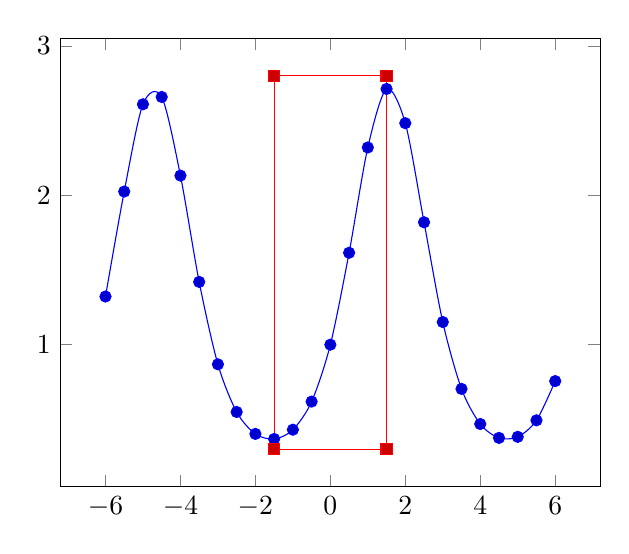
\begin{tikzpicture}[]
\begin{axis}[]
    \addplot+[domain=-6:6,smooth] {exp(sin(deg(x)))};
    \addplot+[] coordinates {
    (-1.5,0.3) (1.5,0.3) (1.5,2.8) (-1.5,2.8) (-1.5,0.3) };
\end{axis}
\end{tikzpicture}
&
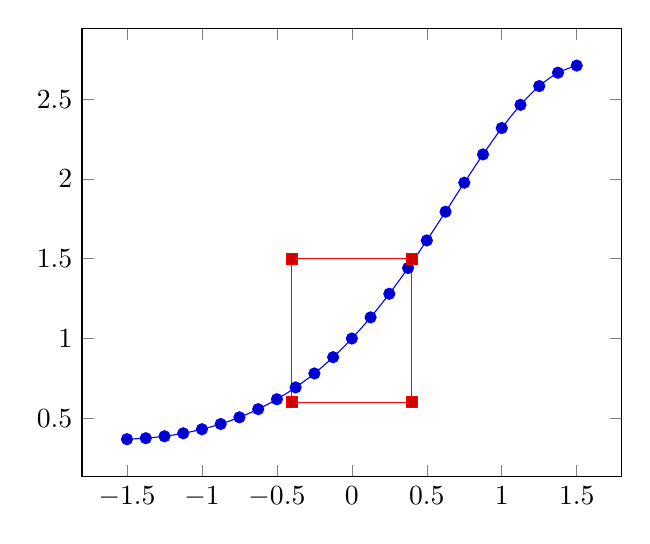
\begin{tikzpicture}[]
\begin{axis}
    \addplot+[domain=-1.5:1.5,smooth] {exp(sin(deg(x)))};
    \addplot+[] coordinates {
    (-0.4,0.6) (0.4,0.6) (0.4,1.5) (-0.4,1.5) (-0.4,0.6) };
\end{axis}
\end{tikzpicture}
\\
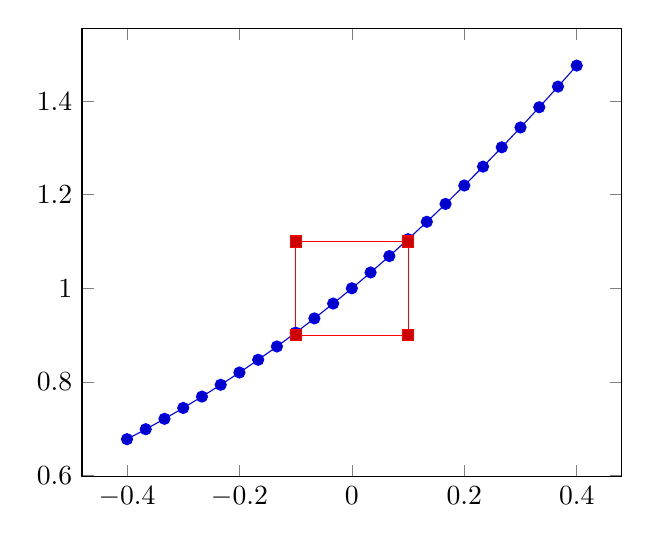
\begin{tikzpicture}[]
\begin{axis}[]
    \addplot+[domain=-0.4:0.4,smooth] {exp(sin(deg(x)))};
    \addplot+[] coordinates {
    (-0.1,0.9) (0.1,0.9) (0.1,1.1) (-0.1,1.1) (-0.1,0.9) };
\end{axis}
\end{tikzpicture}
&
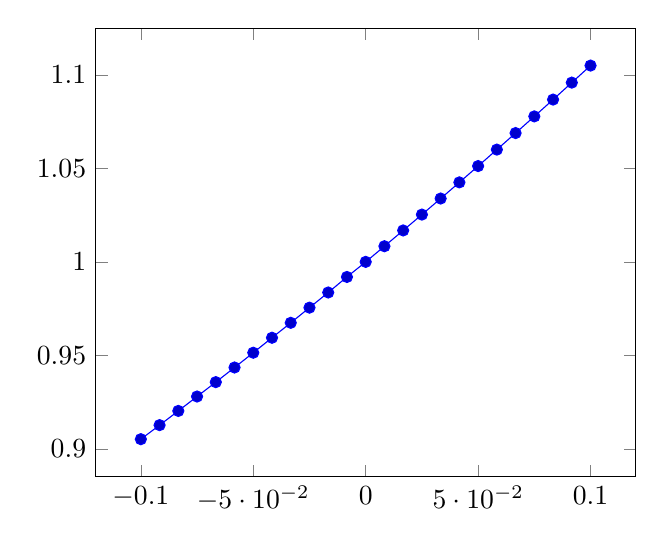
\begin{tikzpicture}[]
\begin{axis}[]
    \addplot+[domain=-0.1:0.1,smooth] {exp(sin(deg(x)))};
\end{axis}
\end{tikzpicture}
\end{tabular}
\caption{zoom in anywhere on any smooth nonlinear curve, such as the plotted~\(f(x)\), and we discover that the curve looks like a straight line on the microscale.
The (red) rectangles show the region plotted in the next graph in the sequence.}
\label{fig:nonlinzoom}
\end{figure}
Linear algebra and equations are also crucial for nonlinear relationships.
\autoref{fig:nonlinzoom} shows four plots of the same nonlinear function, but on successively smaller scales.
Zooming in on the point~\((0,1)\) we see the curve looks straighter and straighter until on the microscale (bottom-right) it is effectively a straight line.
The same is true for everywhere on every smooth nonlinear curve: we discover that every smooth curve looks like a straight line on the microscale. 
Thus we may view any smooth nonlinear function as roughly being made up of lots of microscale straight line segments.
Linear equations and their algebra on this microscale empower our understanding of nonlinear relations---for example, microscale linearity underwrites all of calculus.
 




\endinput






%!TEX root = ../larxxia.tex

\section{Vectors have magnitude and direction}
\label{sec:vhmd}
\secttoc

\begin{quoted}{(Hamlet I.5:159--167)}
There are more things in heaven and earth, Horatio, than are dreamt of in your philosophy.
\end{quoted}

In the eighteenth century, astronomers needed to describe both the position and velocity of the planets. 
Such a description required quantities which have both a magnitude and a direction.
Step outside, a wind blowing at~\(8\)\,m/s from the south-west also has both a magnitude and direction.
Quantities that have the properties of both a magnitude and a direction are called \bfidx{vectors} (from the Latin for \emph{carrier}).

\begin{example}[displacement vector] \label{eg:disvec}
An important class of vectors are the so-called \bfidx{displacement vector}s.
Given two points in space, say~\(A\) and~\(B\), the displacement vector~\(\ovect{AB}\) is the directed line segment from the point~\(A\) to the point~\(B\)---as illustrated by the two displacement vectors \(\ovect{AB}\) and~\(\ovect{CD}\) in the margin.
\newcommand{\tmp}[6]{
  \addplot[blue,thick,quiver={u=#5-#2,v=#6-#3},-stealth] coordinates {(#2,#3)};
  \node[below] at (axis cs:#2,#3) {$#1$};
  \node[below] at (axis cs:#5,#6) {$#4$};}
\newcommand{\temp}[1]{\begin{tikzpicture} 
\begin{axis}[footnotesize,font=\footnotesize
  ,axis equal,  xlabel={$x_1$}, ylabel={$x_2$},
  {\ifnum0=#1 axis lines=none\else axis lines=middle,grid\fi}
  ,xmin=-1.5,xmax=4.5,ymin=-1.7,ymax=3.5
  ] 
  \tmp A12B43
  \tmp C2{-1}D{-1}3
  \ifnum0=#1\else\node[below] at (axis cs:0,0) {\quad$O$};\fi
\end{axis}
\end{tikzpicture}}
\marginpar{\temp0}
For example, if your home is at position~\(A\) and your school at position~\(B\), then travelling from home to school is to move by the amount of the displacement vector~\(\ovect{AB}\).

To be able to manipulate vectors we describe them with numbers.
For such numbers to have meaning they must be set in the context of a \idx{coordinate system}.
So choose an origin for the coordinate system, usually denoted~\(O\), and draw coordinate axes in the plane (or space), as illustrated for the above two \idx{displacement vector}s.
Here the displacement vector~\(\ovect{AB}\) goes three units to the right and one unit up, so we denote it by the ordered pair of numbers~\(\ovect{AB}=(3,1)\).
\marginpar{\temp1}
Whereas the displacement vector~\(\ovect{CD}\) goes three units to the left and four units up, so we denote it by the ordered pair of numbers~\(\ovect{CD}=(-3,4)\).
\end{example}


\needspace{6\baselineskip}
\begin{example}[position vector] \label{eg:posvec}
The next important class of vectors are the \bfidx{position vector}s.
Given some chosen fixed origin in space, then \(\ovect{OA}\)~is the \idx{position vector} of the point~\(A\).
\newcommand{\tmp}[3]{
  \addplot[blue,thick,quiver={u=#2,v=#3},-stealth] coordinates {(0,0)};
  \node[below] at (axis cs:#2,#3) {$#1$};}
\newcommand{\temp}[1]{\begin{tikzpicture} 
\begin{axis}[footnotesize,font=\footnotesize
  ,axis equal, xlabel={$x_1$}, ylabel={$x_2$},
  {\ifnum0=#1 axis lines=none\else axis lines=middle,grid\fi}
  ,xmin=-1.5,xmax=4.5,ymin=-1.7,ymax=3.5
  ] 
  \tmp A12\tmp B43
  \tmp C2{-1}\tmp D{-1}3
  \node[below] at (axis cs:0,0) {\quad$O$};
\end{axis}
\end{tikzpicture}}%
\marginpar{\temp{0}}%
The marginal picture illustrates the position vectors of four points in the plane, given a chosen origin~\(O\).

Again, to be able to manipulate such vectors we describe them with numbers, and such numbers have meaning via a \idx{coordinate system}.
\marginpar{\temp{1}}
So draw coordinate axes in the plane (or space), as illustrated for the above four \idx{position vector}s.
Here the position vector~\(\ovect{OA}\) goes one unit to the right and two units up so we denote it by \(\ovect{OA}=(1,2)\).
Similarly, the position vectors \(\ovect{OB}=(4,3)\),  \(\ovect{OC}=(2,-1)\), and  \(\ovect{OB}=(-1,3)\).
Recognise that the ordered pairs of numbers in the position vectors are exactly the coordinates of each of the specified end-points. 
\end{example}


\begin{example}[\idx{velocity vector}] \label{eg:}
Consider an airplane in level flight at \(900\)\,km/hr to the east-north-east.
\newcommand{\tmp}[3]{
  \addplot[blue,thick,quiver={u=#2,v=#3},-stealth] coordinates {(0,0)};
  \node[above] at (axis cs:#2,#3) {#1};}
\newcommand{\temp}[1]{\begin{tikzpicture} 
\begin{axis}[tiny,font=\footnotesize
  ,axis equal, xlabel={East}, ylabel={North}
  ,axis lines=middle,
  {\ifcase#1 xtick={-9999},ytick={-9999} \or grid\fi}
  ,ymin=-1,xmin=-20,xmax=980,ymax=380
  ] 
  \tmp {\mbox{airplane\quad}}{831.5}{344.4}
  \node[below] at (axis cs:0,0) {\quad$O$};
  \ifcase#1\or
  \tmp {}{831.5}{0}
  \tmp {}{0}{344.4}
  \fi
\end{axis}
\end{tikzpicture}}%
\marginpar{\temp0}%
Choosing coordinate axes oriented to the East and the North, the direction of the airplane is at an angle~\(22.5^\circ\) from the East, as illustrated in the margin.
Trigonometry then tells us that the Eastward part of the speed of the airplane is \(900\cos(22.5^\circ)=831.5\)\,km/hr, whereas the Northward part of the speed is \(900\sin(22.5^\circ)=344.4\)\,km/hr (as indicated in the margin).
\marginpar{\temp1}%
Further, the airplane is in level flight, not going up or down, so in the third direction of space (vertically) its speed component is zero.
Putting these together forms the velocity vector \((831.5,344.4,0)\) in~km/hr in space.

Another airplane takes off from an airport at~\(360\)\,km/hr to the northwest and climbs at~\(2\)\,m/s.
The direction northwest is~\(45^\circ\) to the East-West lines and \(45^\circ\) to the North-South lines.  
Trigonometry then tells us that the Westward speed of the airplane is \(360\cos(45^\circ)=360\cos(\tfrac\pi4)=254.6\)\,km/hr, whereas the Northward speed is \(360\sin(45^\circ)=360\sin(\tfrac\pi4)=254.6\)\,km/hr as illustrated in the margin.
\marginpar{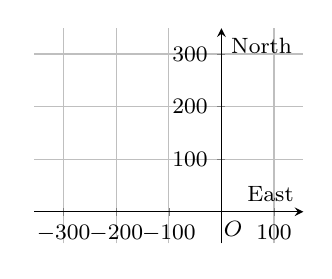
\begin{tikzpicture} 
\begin{axis}[footnotesize,font=\footnotesize
  ,axis equal, xlabel={East}, ylabel={North}
  ,axis lines=middle, grid
  ,ymin=-60,xmin=-299,xmax=99,ymax=349
  ] 
  \tmp {airplane}{-254.6}{254.6}
  \node[below] at (axis cs:0,0) {\quad$O$};
\end{axis}
\end{tikzpicture}}%
But West is the opposite direction to East, so if the coordinate system treats East as positive, then West must be negative.
Consequently, together with the climb in the vertical, the velocity vector is \((-254.6\)\,km/hr,\(254.6\)\,km/hr,\(2\,\)m/s\()\).
But it is best to avoid mixing units within a vector, so here convert all speeds to~m/s: here \(360\)\,km/hr upon dividing by~\(3600\)\,secs/hr and multiplying by \(1000\)\,m/km gives \(360\)\,km/hr\({}=100\)\,m/s.
Then the North and West speeds are both \(100\cos(\tfrac\pi4)=70.71\)\,m/s.
Consequently, the \idx{velocity vector} of the climbing airplane should be described as \((-70.71,70.71,2)\) in~m/s.
\end{example}


In applications, as these examples illustrate, the `physical' vector exists before the coordinate system.
It is only when we choose a specific coordinate system that a `physical' vector gets expressed by numbers.
%When enmeshed deep in the difficulties of learning the marvellous properties of vectors and matrices it is all to easy to forget this important aspect.
Throughout, unless otherwise specified, this book assumes that vectors are expressed in what is called a \bfidx{standard coordinate system}.
\begin{itemize}
\item In the two dimensions of the plane the standard coordinate system has two coordinate axes, 
\marginpar{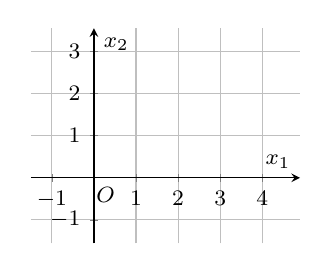
\begin{tikzpicture} 
\begin{axis}[footnotesize,font=\footnotesize
  ,axis equal, axis lines=middle, grid
  , xlabel={$x_1$}, ylabel={$x_2$}
  ,xmin=-1.5,xmax=4.9,ymin=-1.5,ymax=3.5
  ] 
  \node[below] at (axis cs:0,0) {\quad$O$};
\end{axis}
\end{tikzpicture}}%
one horizontal and one vertical at right-angles to each other, often labelled~\(x_1\) and~\(x_2\) respectively (as illustrated in the margin), although labels~\(x\) and~\(y\) are also common.%

\item In the three dimensions of space the standard coordinate system has three coordinate axes, 
\marginpar{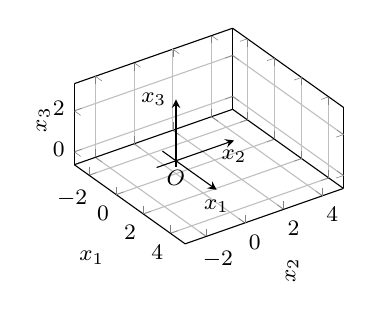
\begin{tikzpicture} 
\begin{axis}[footnotesize,font=\footnotesize,view={55}{30}
  ,axis equal, axis lines=box, grid
  ,xlabel={$x_1$}, ylabel={$x_2$}, zlabel={$x_3$},label shift={-1.5ex}
  ] 
  \node[below] at (axis cs:0,0,0) {$O$};
  \addplot3[black,quiver={u=4,v=0,w=0},-stealth] coordinates {(-1,0,0)};
  \node[below] at (axis cs:3,0,0) {$x_1$};
  \addplot3[black,quiver={u=0,v=4,w=0},-stealth] coordinates {(0,-1,0)};
  \node[below] at (axis cs:0,3,0) {$x_2$};
  \addplot3[black,quiver={u=0,v=0,w=3.3},-stealth] coordinates {(0,0,-0.3)};
  \node[left] at (axis cs:0,0,3) {$x_3$};
\end{axis}
\end{tikzpicture}}%
two horizontal and one vertical all at right-angles to each other, often labelled~\(x_1\), \(x_2\) and~\(x_3\) respectively (as illustrated in the margin), although labels~\(x\), \(y\) and~\(z\) are also common.

\item Correspondingly, in so-called `\(n\)~dimensions' the standard coordinate system has \(n\)~coordinate axes, all at right-angles to each other, and often labelled \hlist xn, respectively.
\end{itemize}




\begin{definition} \label{def:vecs}
Given a \idx{standard coordinate system} with \(n\)~coordinate axes, all at \idx{right-angles} to each other, a \bfidx{vector} is an ordered \(n\)-tuple of real numbers \hlist xn\ equivalently written either as a row in parentheses or as a column in brackets,
\begin{equation*}
(\hlist xn)=\begin{bmatrix} x_1\\x_2\\\vdots\\x_n \end{bmatrix}
\end{equation*}
(they mean the same, it is just more convenient to usually use a row in parentheses in text, and a column in brackets in displayed mathematics).
The real numbers \hlist xn\ are called the \bfidx{components} of the vector, and the number of components is termed its \bfidx{size} (here~\(n\)).
The components are determined such that letting~\(X\) be the point with coordinates \((\hlist xn)\) then the \idx{position vector}~\(\ovect{OX}\) has the same magnitude and direction as the vector denoted \((\hlist xn)\).
\begin{aside}
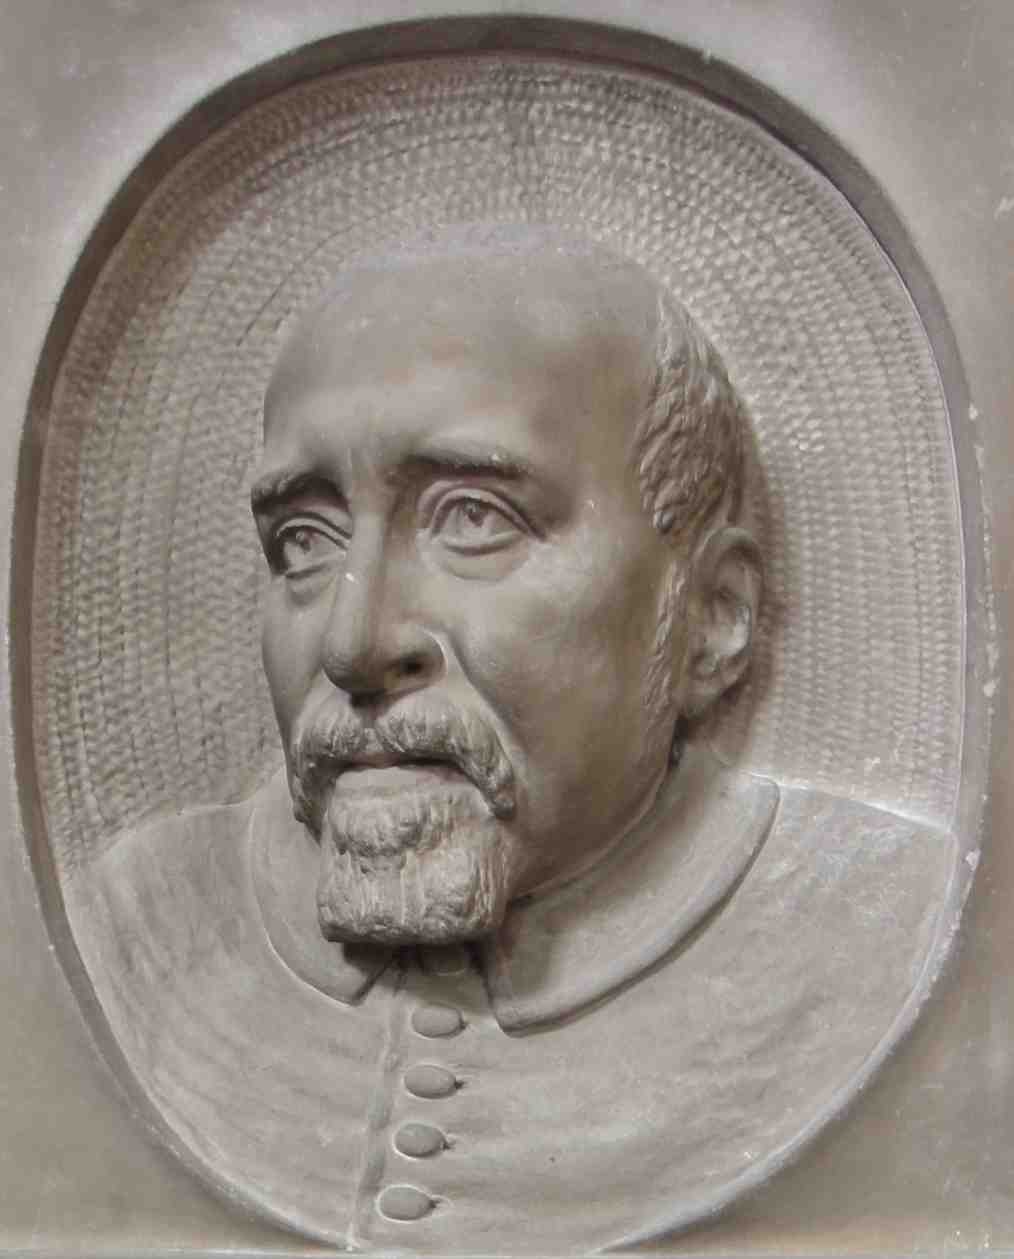
\includegraphics[width=\linewidth]{Vectors/RobertRecorde}
\index{Recorde, Robert}Robert Recorde invented the equal sign circa 1557 ``bicause noe~2 thynges can be moare equalle''.  
%He also invented the term ``sine'' and the method of extracting the square root by hand.
\end{aside}%
Two vectors of the same \idx{size} are \bfidx{equal},~\(=\), if all their corresponding components are equal (vectors with different sizes are never equal).
\end{definition}

Examples~\ref{eg:disvec} and~\ref{eg:posvec} introduced some vectors and wrote them as a row in parentheses, such as \(\ovect{AB}=(3,1)\).
In this book exactly the same thing is meant by the columns in brackets: for example,
\begin{eqnarray*}&&
\ovect{AB}=(3,1)=\begin{bmatrix} 3\\1 \end{bmatrix},\quad
\ovect{CD}=(-3,4)=\begin{bmatrix} -3\\4 \end{bmatrix},\quad
\\&&
\ovect{OC}=(2,-1)=\begin{bmatrix} 2\\-1 \end{bmatrix},\quad
(-70.71,70.71,2)=\begin{bmatrix} -70.71\\70.71\\2 \end{bmatrix}.
\end{eqnarray*}
However, as defined subsequently, a row of numbers within brackets is  quite different: \((3,1)\neq\begin{bmatrix} 3&1 \end{bmatrix}\),  and \((831,344,0)\neq\begin{bmatrix} 831&344&0 \end{bmatrix}\).

The \emph{ordering} of the components is very important.
\marginpar{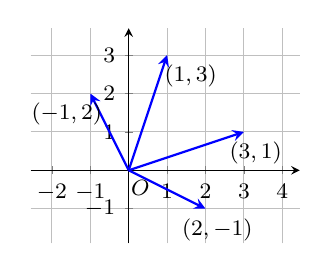
\begin{tikzpicture} 
\newcommand{\tmp}[3]{
  \addplot[blue,thick,quiver={u=#2,v=#3},-stealth] coordinates {(0,0)};
  \node[below] at (axis cs:#2,#3) {$#1$};}
\begin{axis}[footnotesize,font=\footnotesize
  ,axis equal ,axis lines=middle, grid
  ,ymin=-1.9,xmin=-2,xmax=3.9,ymax=3.7
  ] 
  \tmp {\quad(3,1)}31 \tmp {\qquad(1,3)}13
  \tmp {\quad(2,-1)}2{-1} \tmp {(-1,2)\qquad}{-1}2
  \node[below] at (axis cs:0,0) {\quad$O$};
\end{axis}
\end{tikzpicture}}%
For example, as illustrated in the margin, the vector~\((3,1)\) is very different from the vector~\((1,3)\); similarly, the vector~\((2,-1)\) is very different from the vector~\((-1,2)\).
 


\begin{definition} \label{def:rRn}
The set of all vectors with \(n\)~components is denoted~\(\RR^n\)\index{Rn@\(\RR^n\)}.
The vector with all components zero,  \((0,0,\ldots,0)\), is called the \bfidx{zero vector} and denoted by~\ov.
\end{definition}

\begin{example} \label{eg:}
\begin{itemize}
\item All the vectors we can draw and imagine in the two dimensional plane form~\(\RR^2\).  
Sometimes we write that \(\RR^2\)~is the plane because of this very close connection.

\item All the vectors we can draw and imagine in three dimensional space form~\(\RR^3\).  
Again, sometimes we write that \(\RR^3\)~is three dimensional space because of the close connection. 

\item The set~\(\RR^1\) is the set of all vectors with one component, and that one component is measured along one axis.  
Hence \(\RR^1\)~is effectively the same as the set of real numbers labelling that axis.
\end{itemize}
\end{example}


As just introduced for the zero vector~\ov, this book generally denotes vectors by a bold letter (except for displacement vectors).
The other common notation you may see elsewhere is to denote vectors by a small over-arrow such as in the ``zero vector~\(\arrowvec0\)\,''.
Less commonly, some books and articles use an over- or under-tilde~(\(\sim\)) to denote vectors.
Be aware of this different notation in reading other books.



Question: why do we need vectors with \(n\)~components, in~\(\RR^n\), when the world around us is only three dimensional?
Answer: because vectors can encode much more than spatial structure as in the next example. 


\begin{example}[\idx{linguistic vector}s] \label{eg:deflsv}
Consider the following four sentences.
\begin{enumerate}
\item The dog sat on the mat.
\item The cat scratched the dog.
\item The cat and dog sat on the mat.
\item The dog scratched.
\end{enumerate}
These four sentences involve up to three objects, cat, dog and mat, and two actions, sat and scratched.  
Some characteristic of the sentences is captured simply by counting the number of times each of these three objects and two actions appear in each sentence, and then forming a vector from the counts.
Let's use vectors \(\wv=(N_{\text{cat}}, N_{\text{dog}}, N_{\text{mat}}, N_{\text{sat}}, N_{\text{scratched}})\) where the various~\(N\) are the counts of each word (\wv~for words). 
The previous statement implicitly specifies that we use five coordinate axes, perhaps labelled ``cat'', ``dog'', ``mat'', ``sat'' and ``scratched'', and that distance along each axis represents the number of times the corresponding word is used.
These word vectors are in~\(\RR^5\).
Then
\begin{enumerate}
\item ``The dog sat on the mat'' is summarised by the vector \(\wv=(0,1,1,1,0)\).
\item ``The cat scratched the dog'' is summarised by the vector \(\wv=(1,1,0,0,1)\).
\item ``The cat and dog sat on the mat'' is summarised by the vector \(\wv=(1,1,1,1,0)\).
\item ``The dog scratched'' is summarised by the vector \(\wv=(0,1,0,0,1)\).
\item An empty sentence is the \idx{zero vector} \(\wv=(0,0,0,0,0)\).
\item Together, the two sentences ``The dog sat on the mat.
 The cat scratched the dog.'' are summarised by the vector \(\wv=(1,2,1,1,1)\).
\end{enumerate}
Using such crude summary representations of some text, even of entire documents, empowers us to use powerful mathematical techniques to relate documents together, compare and contrast, express similarities, look for type clusters, and so on.
In application we would not just count words for objects (nouns) and actions (verbs), but also qualifications (adjectives and adverbs).\footnote{Look up Latent Semantic Indexing, such as at \url{https://en.wikipedia.org/wiki/Latent_semantic_indexing} [April 2015]}

People generally know and use thousands of words.
Consequently, in practice, such word vectors typically have thousands of components corresponding to coordinate axes of thousands of distinct words.
To cope with such vectors of many components, modern linear algebra has been developed to powerfully handle problems involving vectors with thousands, millions or even an `infinite number' of components.
\end{example}

\begin{table}
\hrule
\begin{minipage}{\linewidth}
\paragraph{King -- man + woman = queen}
\begin{quoted}{Technology Review, 2015}
Computational linguistics has dramatically changed the way researchers study and understand language. 
The ability to number-crunch huge amounts of words for the first time has led to entirely new ways of thinking about words and their relationship to one another.

This number-crunching shows exactly how often a word appears close to other words, an important factor in how they are used. 
So the word Olympics might appear close to words like running, jumping, and throwing but less often next to words like electron or stegosaurus.  
This set of relationships can be thought of as a multidimensional vector that describes how the word Olympics is used within a language, which itself can be thought of as a vector space.  

And therein lies this massive change. 
This new approach allows languages to be treated like vector spaces with precise mathematical properties. 
Now the study of language is becoming a problem of vector space mathematics.
\footnote{\url{http://www.technologyreview.com/view/541356} [Oct 2015]}
\end{quoted}
\end{minipage}
\hrule
\end{table}




\begin{activity}
Given word vectors \(\wv=(N_{\text{cat}}\clb N_{\text{dog}}\clb N_{\text{mat}}\clb N_{\text{sat}}\clb N_{\text{scratched}})\) as in \autoref{eg:deflsv},
which of the following has word vector \(\wv=(2,2,0,2,1)\)?
\actposs[1]
{``A dog sat.  A cat scratched the dog.  The cat sat.''}
{``The dog scratched the cat on the mat.''}
{``A dog and cat both sat on the mat which the dog had scratched.''}
{``Which cat sat by the dog on the mat, and then scratched the dog.''}
%\begin{enumerate}
%\item ``The dog scratched the cat on the mat.''
%\item\actans ``A dog sat.  A cat scratched the dog.  The cat sat.''
%\item ``A dog and cat both sat on the mat which the dog had scratched.''
%\item ``Which cat sat by the dog on the mat, and then scratched the dog.''
%\end{enumerate}
\end{activity}







\begin{definition}[Pythagoras] \label{def:veclen}
For every \idx{vector} \(\vv=(\hlist vn)\) in~\(\RR^n\),
define the \bfidx{length} (or \bfidx{magnitude}) of vector~\vv\  to be the real number~(\(\geq0\))
\index{$\vert\cdot\vert$|textbf} 
\begin{equation*}
|\vv|:=\sqrt{v_1^2+v_2^2+\cdots+v_n^2}\,.
\end{equation*}
A vector of length one is called a \bfidx{unit vector}.
(Many people and books denote the length of a vector with a pair of double lines, as in~\(\|\vv\|\).  Either notation is good.)
\end{definition}


\begin{example} \label{eg:}
Find the lengths of the following vectors.
\begin{parts}
\item \(\av=(-3,4)\)
\begin{solution} 
\(|\av|=\sqrt{(-3)^2+4^2}=\sqrt{25}=5\). 
\end{solution}

\item \(\bv=(3,3)\)
\begin{solution} 
\(|\bv|=\sqrt{3^2+3^2}=\sqrt{18}=3\sqrt2\). 
\end{solution}


\item \(\cv=(1,-2,3)\)
\begin{solution} 
\(|\cv|=\sqrt{1^2+(-2)^2+3^2}=\sqrt{14}\). 
\end{solution}

\item \(\dv=(1,-1,-1,1)\)
\begin{solution} 
\(|\dv|=\sqrt{1^2+(-1)^2+(-1)^2+1^2}=\sqrt4=2\).
\end{solution}
\end{parts}
\end{example}

\begin{example} \label{eg:}
Write down three different vectors, all three with the same number of components, that are (a)~of length~\(5\), (b)~of length~\(3\), and (c)~of length~\(-2\).
\begin{solution} 
\begin{enumerate}
\item Humans knew of the \(3:4:5\) right-angled triangle thousands of years ago, so perhaps one answer could be \((3,4)\), \((-4,3)\) and~\((5,0)\).
\item One answer might be \((3,0,0)\), \((0,3,0)\) and~\((0,0,3)\). 
A more interesting answer might arise from knowing \(1^2+2^2+2^2=3^2\) leading to an answer of \((1,2,2)\), \((2,-1,2)\) and~\((-2,2,1)\).
\item Since the length of a vector is~\(\sqrt{\cdots}\) which is always positive or zero, the length cannot be negative, so there is no possible answer to this last request.
\end{enumerate}
 
\end{solution}
\end{example}




\begin{activity}
What is the length of the vector \((2,-3,6)\)\,?
\actposs[4]{\(7\)}{\(\sqrt{11}\)}{\(5\)}{\(11\)}
%\partswidth=5em
%\begin{parts}
%\item \(\sqrt{11}\)
%\item \(5\)
%\item\actans \(7\)
%\item \(11\)
%\end{parts}
\end{activity}




\begin{theorem} \label{thm:veclen0}
The \idx{zero vector} is the only vector of \idx{length} zero:
 \(|\vv|=0\) if and only if \(\vv=\ov\)\,.
\end{theorem}

\begin{proof} 
First establish the zero vector has length zero.
From \autoref{def:veclen}, in~\(\RR^n\),
\begin{equation*}
|\ov|=\sqrt{0^2+0^2+\cdots+0^2}=\sqrt{0}=0\,.
\end{equation*}
Second, if a vector has length zero then it must be the zero vector.
Let vector \(\vv=(\hlist vn)\) in~\(\RR^n\) have zero length.
By squaring both sides of the \autoref{def:veclen} for length we then know that
\begin{equation*}
\underbrace{v_1^2}_{\geq0}+\underbrace{v_2^2}_{\geq0}
+\cdots+\underbrace{v_n^2}_{\geq0}=0\,.
\end{equation*}
Being squares, all terms on the left are non-negative, so the only way they can all add to zero is if they are all zero.
That is, \(v_1=v_2=\cdots=v_n=0\)\,.
Hence, the vector~\vv\ must be the zero vector~\ov.
\end{proof}






\subsection{Exercises}

\begin{exercise} \label{ex:} 
For each case: on the plot draw the \idx{displacement vector}s \(\ovect{AB}\) and~\(\ovect{CD}\), and the \idx{position vector}s of the points~\(A\) and~\(D\).
\newcommand{\mytemp}{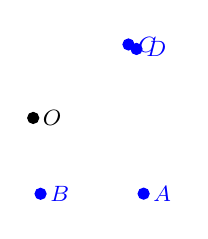
\begin{tikzpicture} 
\begin{axis}[footnotesize,font=\footnotesize
  ,axis equal, xlabel={$x_1$}, ylabel={$x_2$}
  ,axis lines=none  ] 
  \foreach \q in {A,B,C,D} {
    \pgfmathparse{rand*4}\let\h\pgfmathresult
    \pgfmathparse{rand*3}\let\v\pgfmathresult
    \edef\myytmp{\noexpand
    \addplot[blue,mark=*] coordinates {(\h,\v)} node[right] {$\q$};
    \noexpand \addplot[blue,no marks] coordinates {(0.5+\h,1.2*\v)};
    }\myytmp
    };
    \addplot[black,mark=*] coordinates {(0,0)} node[right] {$O$};
\end{axis}
\end{tikzpicture}}

\begin{parts}
\pgfmathsetseed{9091}
\item \mytemp
\item \mytemp
\item \mytemp
\item \mytemp
\item \mytemp
\item \mytemp
\end{parts}
\end{exercise}




\begin{exercise} \label{ex:fourvec} 
For each case: roughly estimate (to say~\(\pm 0.2\)) each of the two \idx{components} of the four \idx{position vector}s of the points~\(A\), \(B\), \(C\) and~\(D\).
\newcommand{\mytemp}{\edef\mytempans{}%
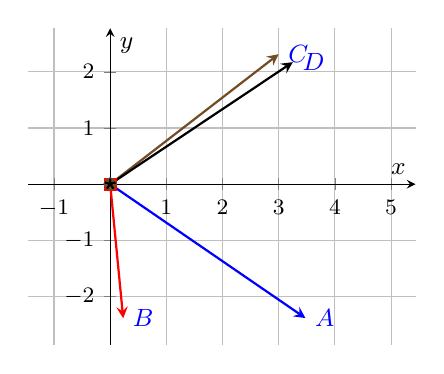
\begin{tikzpicture}
\pgfkeys{/pgf/number format/precision=1,/pgf/number format/fixed}
\begin{axis}[small,font=\small
  ,axis equal, xlabel={$x$}, ylabel={$y$}
  ,axis lines=middle, grid  ] 
  \foreach \q in {A,B,C,D} {
    \pgfmathparse{rand*4}\let\h\pgfmathresult
    \pgfmathprintnumberto{\pgfmathresult}{\twoh}
    \pgfmathparse{rand*3}\let\v\pgfmathresult
    \pgfmathprintnumberto{\pgfmathresult}{\twov}
    \global\edef\mytempans{\mytempans \q(\twoh,\twov)\ }
    \edef\myytmp{\noexpand
    \addplot+[quiver={u=\h,v=\v},-stealth,thick] 
    coordinates {(0,0)};
    \noexpand \node[blue,right] at (axis cs:\h,\v) {$\q$};
    \noexpand \addplot[blue,no marks,forget plot] coordinates {(0.5+\h,1.2*\v)};
    }\myytmp
    };
\end{axis}
\end{tikzpicture}%
\answer{\mytempans}
}
\begin{enumerate}
\pgfmathsetseed{3034}
\item \mytemp
\item \mytemp
\item \mytemp
\item \mytemp
\item \mytemp
\item \mytemp
\end{enumerate}
\end{exercise}



\begin{exercise} \label{ex:} 
For each case plotted in \autoref{ex:fourvec}:
from your estimated components of each of the four position vectors, calculate the \idx{length} (or \idx{magnitude}) of the four vectors. 
Also use a ruler (or otherwise) to directly measure an estimate of the length of each vector.
Confirm your calculated lengths reasonably approximate your measured lengths.
\end{exercise}



\begin{exercise} \label{ex:8siambks} 
Below are the titles of eight books that The Society of Industrial and Applied Mathematics (\textsc{siam}) reviewed recently.
\begin{enumerate}
\item Introduction to Finite and Spectral Element Methods using MATLAB
\item Derivative Securities and Difference Methods 
\item Iterative Methods for Linear Systems: Theory and Applications 
\item Singular Perturbations: Introduction to System Order Reduction Methods with Applications 
\item Risk and Portfolio Analysis: Principles and Methods 
\item Differential Equations: Theory, Technique, and Practice 
\item Contract Theory in Continuous-Time Models 
\item Stochastic Chemical Kinetics: Theory and Mostly Systems Biology Applications
\end{enumerate}
Make a list of the five significant words that appear more than once in this list (not including the common nontechnical words such as ``and'' and ``for'', and not distinguishing between words with a common root).
Being consistent about the order of words, represent each of the eight titles by a \idx{word vector} in~\(\RR^5\).

%\verb#tr -cs "[:alpha:]" "\n" < books.txt |sort -f#
\answer{Application, Introduction, Method, System, Theory.
\(\av=(0,1,1,0,0)\),
\(\bv=(0,0,1,0,0)\),
\(\cv=(1,0,1,1,1)\),
\(\dv=(1,1,1,1,0)\),
\(\ev=(0,0,1,0,0)\),
\(\fv=(0,0,0,0,1)\),
\(\gv=(0,0,0,0,1)\),
\(\hv=(1,0,0,1,1)\)}
\end{exercise}





\begin{exercise} \label{ex:} 
In a few sentences, answer\slash discuss each of the the following.
\begin{enumerate}
\item Why is a coordinate system important for a vector?

\item Describe the distinction between a displacement vector and a position vector.

\item Why do two vectors have to be the same size in order to be equal?

\item What is the connection between the length of a vector and Pythagoras' theorem for triangles?

\item Describe a problem that would occur if the ordering of the components in a vector was not significant?

\item Recall that a vector has both a magnitude and a direction.  
Comment on why the zero vector is the only vector with zero magnitude.

\item In what other courses have you seen vectors?  What was the same and what was different?

\end{enumerate}
\end{exercise}





\begin{comment}%{ED498555.pdf}
why, what caused X?
how did X occur?
what-if? what-if-not?
how does X compare with Y?
what is the evidence for X?
why is X important?
\end{comment}






%!TEX root = ../larxxia.tex

\section{Adding and stretching vectors}
\label{sec:asv}
\secttoc


We want to be able to make sense of statements such as ``king --~man +~women =~queen''.
To do so, we need to define operations on vectors.
Useful operations on vectors are those that are physically meaningful.
Then our algebraic manipulations derive powerful results in applications.
The first two vector operations are addition and \text{scalar multiplication.}


\subsection{Basic operations}

\begin{example} \label{eg:vecadd} 
Vectors of the same \idx{size} are added component-wise.
Equivalently, obtain the same result by geometrically joining the two vectors `head-to-tail' and drawing the vector from the start to the finish.
\begin{enumerate}[ref=\ref{eg:vecadd}(\alph*)]
\newcommand{\tmp}[3]{
  \addplot[blue,thick,quiver={u=#2,v=#3},-stealth] coordinates {(0,0)};
  \node[right] at (axis cs:#2,#3) {$#1$};}
  
\item\label[example]{eg:vecadda} Let's add the two vectors shown below-left:
\((1,3)+(2,-1)=(1+2,3+(-1))=(3,2)\) as illustrated below-middle, where 
the vector~\((2,-1)\) is drawn from the end of \((1,3)\), and the end-point of the result determines the vector addition~\((3,2)\).
\begin{center}
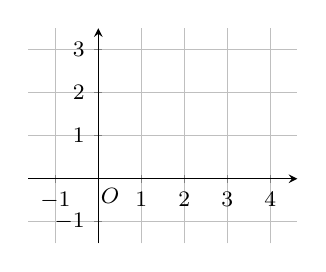
\begin{tikzpicture} 
\begin{axis}[footnotesize,font=\footnotesize
  ,axis equal, axis lines=middle, grid
  ,ymin=-1.5,xmin=-0.5,xmax=3.5,ymax=3.5
  ] 
  \tmp {(1,3)}13 
  \tmp {(2,-1)}2{-1}
  \node[below] at (axis cs:0,0) {\quad$O$};
\end{axis}
\end{tikzpicture}
\hfil
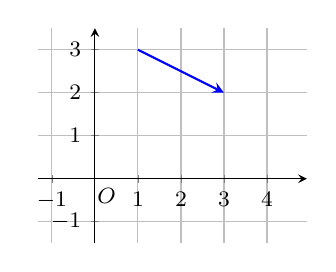
\begin{tikzpicture} 
\begin{axis}[footnotesize,font=\footnotesize
  ,axis equal, axis lines=middle, grid
  ,ymin=-1.5,xmin=-0.5,xmax=4.1,ymax=3.5
  ] 
  \tmp {(1,3)}13 
  \tmp {(2,-1)}2{-1}
  \tmp {(3,2)}32
  \addplot[blue,thick,quiver={u=2,v=-1},-stealth] coordinates {(1,3)};
  \node[below] at (axis cs:0,0) {\quad$O$};
\end{axis}
\end{tikzpicture}
\hfil
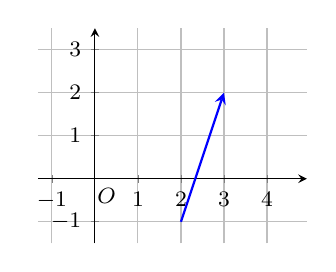
\begin{tikzpicture} 
\begin{axis}[footnotesize,font=\footnotesize
  ,axis equal, axis lines=middle, grid
  ,ymin=-1.5,xmin=-0.5,xmax=4.1,ymax=3.5
  ] 
  \tmp {(1,3)}13 
  \tmp {(2,-1)}2{-1}
  \tmp {(3,2)}32
  \addplot[blue,thick,quiver={u=1,v=3},-stealth] coordinates {(2,-1)};
  \node[below] at (axis cs:0,0) {\quad$O$};
\end{axis}
\end{tikzpicture}
\end{center}
This result~\((3,2)\) is the same if the vector~\((1,3)\) is drawn from the end of~\((2,-1)\) as shown above-right.
That is, \((2,-1)+(1,3)=(1,3)+(2,-1)\).
That the order of addition is immaterial is the \idx{commutative law} of vector addition. 
\cref{thm:vecopsa} establishes this law \text{in general.}

\newcommand{\temp}[2]{\begin{tikzpicture} 
\begin{axis}[footnotesize,font=\footnotesize,view={#2}{30}
  ,axis equal, axis lines=box,zmax=3.5
  ,xlabel={$x_1$}, ylabel={$x_2$}, zlabel={$x_3$},label shift={-1.5ex}
  ] 
  \node[below] at (axis cs:0,0,0) {$O$};
  \threevec[below]320
  \threevec{-1}32
  \ifnum0<#1
  \addplot3[blue,thick,quiver={u=-1,v=3,w=2},-stealth] coordinates {(3,2,0)};
  \addplot3[blue,thick,quiver={u=3,v=2,w=0},-stealth] coordinates {(-1,3,2)};
  \threevec252
\fi
\end{axis}
\end{tikzpicture}}
\needlines{6}%
\begin{figbox}{\temp0{55}}%
\item \((3,2,0)+(-1,3,2)=(3+(-1),2+3,0+2)=(2,5,2)\)  as illustrated below where (given the two vectors as plotted to the right) 
the vector~\((-1,3,2)\) is drawn from the end of~\((3,2,0)\), and the end-point of the result determines the vector addition~\((2,5,2)\).
As below, find the same result by drawing the vector~\((3,2,0)\) from the end of~\((-1,3,2)\).
\end{figbox}
\begin{center}
 \temp1{50}\temp1{55}%draw stereo pair
\end{center}
As drawn above, many of the three-D plots in this book are \bfidx{stereo pair}s, drawing the plot from two slightly different viewpoints:\footnote{I implement such cross-eyed stereo so that these stereo images are useful both printed and when projected on a screen.} cross your eyes to merge two of the images, and then focus on the pair of plots to see the 3D effect.
With practice viewing such 3D stereo pairs becomes less difficult!%
\footnote{To help keeping your eyes crossed while you try to focus on the plots, hold a finger or pen in front of your nose so that your right-eye sight across the top of the finger\slash pen aligns with the centre of the left-picture, and simultaneously your left-eye sight  across the top of the finger\slash pen aligns with the centre of the right-picture.}

\item The addition \((1,3)+(3,2,0)\) is not defined and cannot be done because the two vectors have a different number of components; they have different sizes.
\end{enumerate}
\end{example}




\begin{example} 
To multiply a vector by a \index{scalar multiplication}scalar, a number, multiply each component by the scalar. 
Equivalently, visualize the result through stretching the vector by a factor of the scalar.
\begin{enumerate}
\needlines{4}
\item \begin{figbox}{\begin{tikzpicture} 
\newcommand{\tmp}[3]{
  \addplot[blue,thick,quiver={u=#2,v=#3},-stealth] coordinates {(0,0)};
  \node[above] at (axis cs:#2,#3) {$#1$};}
\begin{axis}[footnotesize,font=\footnotesize
  ,axis equal, axis lines=middle, grid
  ,xmin=-6.5,xmax=6.9
  ] 
  \tmp {\uv}32 
  \tmp{2\uv}64
  \tmp{\tfrac13\uv}1{0.667}
  \tmp{-1.5\uv\quad}{-4.5}{-3}
  \node[below] at (axis cs:0,0) {\quad$O$};
\end{axis}
\end{tikzpicture}}%
Let the vector \(\uv=(3,2)\) then, as illustrated to the right,
\begin{eqnarray*}&&
2\uv=2(3,2) =(2\cdot3,2\cdot2) =(6,4),
\\&&
\tfrac13\uv=\tfrac13(3,2) =(\tfrac13\cdot3,\tfrac13\cdot2) =(1,\tfrac23),
\\&&
(-1.5)\uv =(-1.5\cdot3,-1.5\cdot2) =(-4.5,-3).
\end{eqnarray*}
\end{figbox}

\item Let the vector \(\vv=(2,3,1)\) then, as illustrated below in cross-eyed stereo,
\begin{eqnarray*}&&
2\vv=2\begin{bmatrix} 2\\3\\1 \end{bmatrix}
=\begin{bmatrix} 2\cdot2\\2\cdot3\\2\cdot1 \end{bmatrix}
=\begin{bmatrix} 4\\6\\2 \end{bmatrix},
\\&& 
(-\tfrac12)\vv=-\frac12\begin{bmatrix} 2\\3\\1 \end{bmatrix}
=\begin{bmatrix} -\frac12\cdot2\\-\frac12\cdot3\\-\frac12\cdot1 \end{bmatrix}
=\begin{bmatrix} -1\\-\frac32\\-\frac12 \end{bmatrix}. 
\end{eqnarray*}
\begin{center}
\qview{50}{55}{
\begin{tikzpicture} 
\begin{axis}[footnotesize,font=\footnotesize,view={\q}{30}
  ,axis equal, axis lines=box
  ,ymax=6.9,ymin=-1.9,zmax=2,zmin=-1,xmax=4,xmin=-1
  ,xlabel={$x_1$}, ylabel={$x_2$}, zlabel={$x_3$},label shift={-1.5ex}
  ] 
  \node[below] at (axis cs:0,0,0) {$O$};
  \threev231{\vv}
  \threev462{2\vv}
  \threev{-1}{-1.5}{-0.5}{\quad-\frac12\vv}
\end{axis}
\end{tikzpicture}}
\end{center}
\end{enumerate}
\end{example}



\begin{activity}
Combining multiplication and addition, what is \(\uv+2\vv\) for vectors \(\uv=(4,1)\) and \(\vv=(-1,-3)\)?
\actposs[4]{\((2,-5)\)}{\((1,-8)\)}{\((3,-2)\)}{\((5,-8)\)}
\end{activity}



\begin{definition} \label{def:vecops}
Let two vectors in~\(\RR^n\) be \(\uv=(\hlist un)\) and \(\vv=(\hlist vn)\), and let \(c\)~be a \idx{scalar}.
Then the \bfidx{sum} or \bfidx{addition} of~\uv\ and~\vv, denoted \(\uv+\vv\), is the vector obtained by joining~\vv\ to~\uv\ `head-to-tail', and is computed as
\begin{equation*}
\uv+\vv:=(u_1+v_1,u_2+v_2,\ldots,u_n+v_n).
\end{equation*}
The \bfidx{scalar multiplication} of~\uv\ by~\(c\), denoted~\(c\uv\),  is the vector of \idx{length}~\(|c||\uv|\) in the direction of~\uv\ when \(c>0\) but in the opposite direction when \(c<0\), and is computed as
\begin{equation*}
c\uv:=(cu_1,cu_2,\ldots,cu_n).
\end{equation*}
The \bfidx{negative} of~\uv\, denoted~\(-\uv\), is defined as the scalar multiple \(-\uv:=(-1)\uv\), and is a vector of the same \idx{length} as~\uv\ but in exactly the opposite direction.
The \bfidx{difference} \(\uv-\vv\) is defined as the sum \(\uv+(-\vv)\) and is equivalently the vector drawn from the end of~\vv\ to the end of~\uv.
\end{definition}


\begin{wrapfigure}r{0pt}
\vecops01321
\end{wrapfigure}
\begin{example} 
For the vectors~\uv\ and~\vv\ shown to the right, draw the vectors
\(\uv+\vv\), \(\vv+\uv\), \(\uv-\vv\), \(\vv-\uv\), \(\tfrac12\uv\), and~\(-\vv\).

\begin{solution} Drawn below.
\needlines{9}
\begin{Parts}
\item $\uv+\vv$ \vecops11321
\item $\vv+\uv$ \vecops21321
\item $\uv-\vv$ \vecops31321
\item $\vv-\uv$ \vecops41321
\item $\tfrac12\uv$ \vecops51321
\item $-\vv$ \vecops61321
\end{Parts}
\end{solution}
\end{example}


%\begin{wrapfigure}r{0pt} \vecops45{-2}14 \end{wrapfigure}
\begin{activity}[\vecops45{-2}14]
For the vectors~\uv\ and~\vv\ shown to the right, what is the result vector, which is also shown?
\actposs[4]{\(\vv-\uv\)}{\(\uv+\vv\)}{\(\vv+\uv\)}{\(\uv-\vv\)}
\vspace{1ex}
\end{activity}



\begin{wrapfigure}r{0pt}
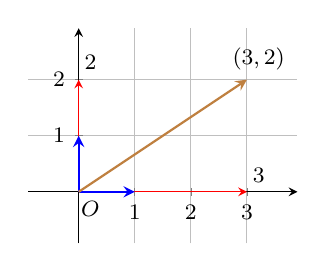
\begin{tikzpicture} 
\newcommand{\tmp}[4]{
  \addplot[#4,quiver={u=#2,v=#3},-stealth] coordinates {(0,0)};
  \node[above] at (axis cs:#2,#3) {$\quad#1$};}
\begin{axis}[footnotesize,font=\footnotesize
  ,axis equal, axis lines=middle, grid
  ,ymin=-0.9,xmin=-0.9,xmax=3.9,ymax=2.9
  ] 
  \node[below] at (axis cs:0,0) {\quad$O$};
  \tmp {3\iv}30{red}
  \tmp {2\jv}02{red}
  \tmp {\iv}10{blue,thick}
  \tmp {\jv}01{blue,thick}
  \tmp {(3,2)}32{brown,thick}
\end{axis}
\end{tikzpicture}\end{wrapfigure}%
Using vector addition and \idx{scalar multiplication}, we often write vectors in terms of so-called \idx{standard unit vector}s.
In the plane, as drawn right, are the two \idx{unit vector}s~\iv\ and~\jv\ defined to be of length one and in the direction of the two \idx{coordinate axes}, respectively.
Hence \(\iv=(1,0)\) and \jv=(0,1), as shown.
\index{i@$\iv$}\index{j@$\jv$}%
Then, for example,
\begin{eqnarray*}
(3,2)&=&(3,0)+(0,2)\quad(\text{by addition})
\\&=&3(1,0)+2(0,1)\quad(\text{by scalar mult})
\\&=&3\iv+2\jv \quad(\text{by definition of \iv\ and \jv}).
\end{eqnarray*}
\index{i@$\iv$}\index{j@$\jv$}\index{k@$\kv$}%
Similarly, in three-dimensional space, we often write vectors in terms of the three vectors~\iv, \jv, and~\kv, defined to be each of \idx{length} one, aligned along the three \idx{coordinate axes}.
Hence \(\iv=(1,0,0)\), \(\jv=(0,1,0)\), and \kv=(0,0,1).
For example,
\begin{eqnarray*}
(2,3,-1)&=&(2,0,0)+(0,3,0)+(0,0,-1)\quad(\text{by addition})
\\&=&2(1,0,0)+3(0,1,0)-(0,0,1)\quad(\text{by scalar mult})
\\&=&2\iv+3\jv-\kv \quad(\text{by definition of \iv, \jv, and \kv}).
\end{eqnarray*}
The next definition generalizes these standard unit vectors to vectors in~\(\RR^n\) for every size~\(n\).


\begin{figbox}{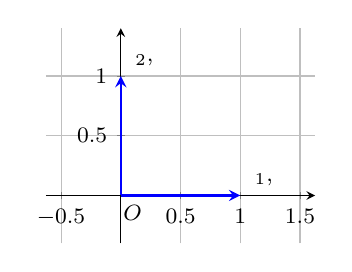
\begin{tikzpicture} 
\newcommand{\tmp}[3]{
  \addplot[blue,thick,quiver={u=#2,v=#3},-stealth] coordinates {(0,0)};
  \node[above] at (axis cs:#2,#3) {$\qquad#1$};}
\begin{axis}[footnotesize,font=\footnotesize
  ,axis equal, axis lines=middle, grid
  ,ymin=-0.4,xmin=-0.5,xmax=1.5,ymax=1.4
  ] 
  \tmp {\ev_1,\iv}10 
  \tmp {\ev_2,\jv}01 
  \node[below] at (axis cs:0,0) {\quad$O$};
\end{axis}
\end{tikzpicture}}%
\begin{definition} \label{def:stuniv}
Given a \idx{standard coordinate system} with \(n\)~\idx{coordinate axes}, all at \idx{right-angles} to each other, the \bfidx{standard unit vector}s \index{e@$\ev_j$|textbf}\(\hlist\ev n\) are the vectors of \idx{length} one in the direction of the corresponding coordinate axis (as illustrated to the right for~\(\RR^2\) and below for~\(\RR^3\)).
That is,
\begin{equation*}
\ev_1=\begin{bmatrix} 1\\0\\\vdots\\0 \end{bmatrix},\quad
\ev_2=\begin{bmatrix} 0\\1\\\vdots\\0 \end{bmatrix},\quad\ldots,\quad
\ev_n=\begin{bmatrix} 0\\0\\\vdots\\1 \end{bmatrix}.
\end{equation*}
In \(\RR^2\) and~\(\RR^3\), the symbols~\index{i@$\iv$|textbf}\iv, \index{j@$\jv$|textbf}\jv, and~\index{k@$\kv$|textbf}\kv\ are often used as synonyms for~\(\ev_1\), \(\ev_2\), and~\(\ev_3\), respectively (as illustrated below).
\end{definition}
\end{figbox}
\begin{center}
\qview{50}{55}{\begin{tikzpicture} 
\begin{axis}[footnotesize,font=\footnotesize,view={\q}{30}
  ,axis equal, axis lines=box, grid,zmax=1.4
  ,xlabel={$x_1$},ylabel={$x_2$},zlabel={$x_3$},label shift={-1.5ex}
  ] 
  \node[below] at (axis cs:0,0,0) {$O$};
  \addplot3[blue,thick,quiver={u=1,v=0,w=0},-stealth] coordinates {(0,0,0)};
  \node[below] at (axis cs:1,0,0) {$\quad\ev_1,\iv$};
  \addplot3[blue,thick,quiver={u=0,v=1,w=0},-stealth] coordinates {(0,0,0)};
  \node[below] at (axis cs:0,1,0) {$\quad\ev_2,\jv$};
  \addplot3[blue,thick,quiver={u=0,v=0,w=1},-stealth] coordinates {(0,0,0)};
  \node[left] at (axis cs:0,0,1) {$\ev_3,\kv$};
\end{axis}
\end{tikzpicture}}
\end{center}

That is, for three examples, the following are equivalent ways of writing the same vector:
\begin{eqnarray*}\bullet&&
(3,2)=\begin{bmatrix} 3\\2 \end{bmatrix}=3\iv+2\jv=3\ev_1+2\ev_2\,;
\\\bullet&&
(2,3,-1)=\begin{bmatrix} 2\\3\\-1 \end{bmatrix}
=2\iv+3\jv-\kv=2\ev_1+3\ev_2-\ev_3\,;
\\\bullet&&
(0,-3.7,0,0.1,-3.9)
=\begin{bmatrix} 0\\-3.7\\0\\0.1\\-3.9 \end{bmatrix}
=-3.7\ev_2+0.1\ev_4-3.9\ev_5\,.
\end{eqnarray*}




\begin{activity}
Which of the following is the same as the vector \(3\ev_2+\ev_5\)?
\actposs[4]{\((0,3,0,0,1)\)}{\((3,1)\)}{\((5,0,2)\)}{\((0,3,0,1)\)}
\end{activity}




\subsection{Distance}
\index{distance|(}
Defining a `distance' between vectors empowers us to concisely compare vectors.

\needlines{7}
\begin{wrapfigure}r{0pt}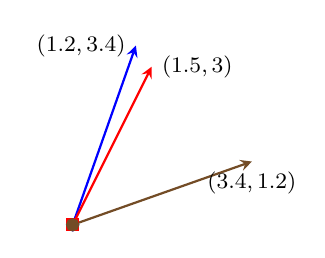
\begin{tikzpicture}
\begin{axis}[footnotesize,font=\footnotesize
,axis equal,axis lines=none,thick]
\addplot+ [quiver={u=1.2,v=3.4},-stealth] coordinates {(0,0)};
\node[left] at (axis cs:1.2,3.4) {$(1.2,3.4)$};
\addplot+ [quiver={u=1.5,v=3},-stealth] coordinates {(0,0)};
\node[right] at (axis cs:1.5,3) {$(1.5,3)$};
\addplot+ [quiver={u=3.4,v=1.2},-stealth] coordinates {(0,0)};
\node[below] at (axis cs:3.4,1.2) {$(3.4,1.2)$};
\end{axis}
\end{tikzpicture}\end{wrapfigure}
\begin{example} 
We would like to say that \((1.2,3.4)\approx(1.5,3)\) to an error~\(0.5\) (as illustrated to the right).
Why is the error~\(0.5\)?  
Because the \idx{difference} between the vectors \((1.5,3)-(1.2,3.4)=(0.3,-0.4)\) has length \(\sqrt{0.3^2+(-0.4)^2}=0.5\)\,.

Conversely, we would like to recognize that vectors \((1.2,3.4)\) and \((3.4,1.2)\) are very different (as also illustrated)---there is a large `distance' between them.
Why is there a large `distance'?  Because the difference between the vectors \((1.2,3.4)-(3.4,1.2)=(-2.2,2.2)\) has length \(\sqrt{(-2.2)^2+2.2^2}=2.2\sqrt2=3.1113\), which is relatively large.
\end{example}

This concept of distance between two vectors~\uv\ and~\vv, directly corresponding to the distance between two points, is the length \(|\uv-\vv|\).

\begin{definition} \label{def:vecdist}
The \bfidx{distance} between vectors~\uv\ and~\vv\ in~\(\RR^n\) is the \idx{length} of their \idx{difference}, \(|\uv-\vv|\).
\end{definition}

\needlines{8}
\begin{wrapfigure}r{0pt}
\qview{30}{35} {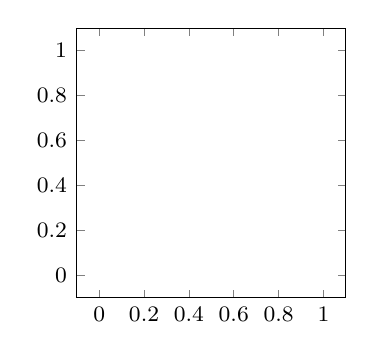
\begin{tikzpicture}
\begin{axis}[footnotesize,font=\footnotesize,height=5cm
,axis equal,axis lines=box,view={\q}{25}]
\threev32{-2}\av
\threev554\bv
\threev7{-2}5\cv
\end{axis}
\end{tikzpicture}}
\end{wrapfigure}
\begin{example} 
Given three vectors \(\av=3\iv+2\jv-2\kv\), \(\bv=5\iv+5\jv+4\kv\), and \(\cv=7\iv-2\jv+5\kv\) (shown right in stereo) use the concept of distance between vectors to answer the following: which pair are the closest to each other? And which pair are furthest from each other?
\par
\begin{solution} 
Compute the distances between each pair.
\begin{itemize}
\item \(|\bv-\av|=|2\iv+3\jv+6\kv| =\sqrt{2^2+3^2+6^2} =\sqrt{49} =7\).
\item \(|\cv-\av|=|4\iv-4\jv+7\kv| =\sqrt{4^2+(-4)^2+7^2} =\sqrt{81} =9\).
\item \(|\cv-\bv|=|2\iv-7\jv-\kv| =\sqrt{2^2+(-7)^2+(-1)^2} =\sqrt{54} =7.3485\)\,.
\end{itemize}
The smallest distance of~\(7\) is between~\av\ and~\bv\ so these two are the closest pair of vectors.
The largest distance of~\(9\) is between~\av\ and~\cv\ so these two are the furthest pair of vectors.
\end{solution}
\end{example}

\begingroup
\def\temp{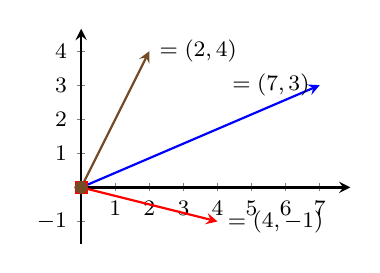
\begin{tikzpicture}
\begin{axis}[footnotesize,font=\footnotesize
,axis equal,axis lines=middle, thick,xmax=7.9]
\addplot+ [quiver={u=7,v=3},-stealth] coordinates {(0,0)};
\node[left] at (axis cs:7,3) {$\av=(7,3)$};
\addplot+ [quiver={u=4,v=-1},-stealth] coordinates {(0,0)};
\node[right] at (axis cs:4,-1) {$\bv=(4,-1)$};
\addplot+ [quiver={u=2,v=4},-stealth] coordinates {(0,0)};
\node[right] at (axis cs:2,4) {$\cv=(2,4)$};
\end{axis}
\end{tikzpicture}}
\begin{activity}[\temp]
%for i=1:999,x=0+round(randn(3,2)*3);y=[0 1 -1;-1 0 1;1 -1 0]*x;d=sqrt(y.^2*[1;1]);if std(d)<0.5, x=x,d=d,break, end, end
Which pair of the following vectors are closest---have the smallest distance between them?  \(\av=(7,3)\), \(\bv=(4,-1)\), \(\cv=(2,4)\)
\actposs{\av, \bv}{\av, \cv}{\bv, \cv}{two of the pairs}
\end{activity}
\endgroup


\index{distance|)}







\subsection{Parametric equation of a line}
\label{sec:pel}

We are familiar with lines in the plane, and equations that describe them. 
Let's now consider such equations from a vector view.
The insights empower us to generalize the descriptions to lines in space, and then to lines in any number of dimensions.

\begin{wrapfigure}[6]r{0pt} 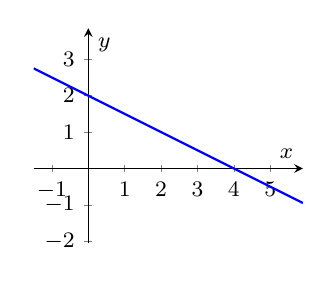
\begin{tikzpicture} 
\begin{axis}[footnotesize,font=\footnotesize
  ,axis equal, axis lines=middle, domain=-1.5:5.9
  ,xlabel={$x$},ylabel={$y$}
  ] 
\addplot+[thick,no marks] {2-x/2};
\end{axis}
\end{tikzpicture}
\end{wrapfigure}
\begin{example} 
Consider the line drawn to the right in some chosen coordinate system.
Recall that one way to find an equation of the line is to find the intercepts with the axes, here at \(x=4\) and at \(y=2\)\,, then write down \(\frac x4+\frac y2=1\) as an equation of the line.
Algebraic rearrangement gives various other forms, such as \(x+2y=4\) or \(y=2-x/2\)\,.

\needlines7
\begin{wrapfigure}r{0pt}
\begin{tikzpicture} 
\begin{axis}[footnotesize,font=\footnotesize
  ,axis equal, axis lines=middle, domain=-1.5:5.9
  ,xlabel={$x$},ylabel={$y$}
  ] 
\node[below] at (axis cs:0,0) {\quad$O$};
\addplot[blue,no marks] {2-x/2};
\addplot[mark=*] coordinates {(2,1)} node[above] {$P$};
\addplot[red,thick,quiver={u=2,v=1},-stealth] coordinates {(0,0)};
\node[above] at (axis cs:1,0.3) {$\pv$};
\addplot[red,thick,quiver={u=-2,v=1},-stealth] coordinates {(2,1)};
\node[above] at (axis cs:1,1.5) {$\dv$};
\addplot[red,thick,quiver={u=1,v=-1/2},-stealth] coordinates {(2,1)};
\node[above] at (axis cs:3,0.3) {$\quad-\tfrac12\dv$};
\end{axis}
\end{tikzpicture}
\end{wrapfigure}%
The alternative is to describe the line with vectors.
Choose any point~\(P\) on the line, such as~\((2,1)\) as drawn to the right.
Then view every other point on the line as having \idx{position vector} that is the vector \idx{sum} of~\(\ovect{OP}\) and a vector aligned along the line.
Denote~\(\ovect{OP}\) by~\pv\ as drawn.
Then, for example, the point~\((0,2)\) on the line has position vector  \(\pv+\dv\) for vector \(\dv=(-2,1)\) because \(\pv+\dv=(2,1)+(-2,1)=(0,2)\).
Other points on the line are also given using the same vectors, \pv\ and~\dv: for example, the point~\((3,\tfrac12)\) has position vector \(\pv-\tfrac12\dv\) (as drawn) because \(\pv-\tfrac12\dv=(2,1)-\tfrac12(-2,1)=(3,\tfrac12)\); and the point~\((-2,3)\) has position vector \(\pv+2\dv=(2,1)+2(-2,1)\).
In general, every point on the line may be expressed as \(\pv+t\dv\) for some scalar~\(t\).

\needlines7
\begin{wrapfigure}r{0pt}
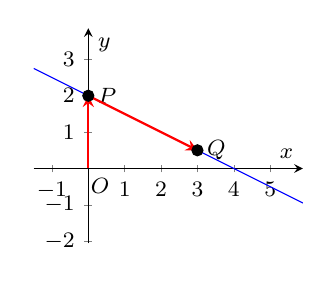
\begin{tikzpicture} 
\begin{axis}[footnotesize,font=\footnotesize
  ,axis equal, axis lines=middle, domain=-1.5:5.9
  ,xlabel={$x$},ylabel={$y$}
  ] 
\node[below] at (axis cs:0,0) {\quad$O$};
\addplot[blue,no marks] {2-x/2};
\addplot[mark=*] coordinates {(0,2)} node[right] {$P$};
\addplot[mark=*] coordinates {(3,0.5)} node[right] {$Q$};
\addplot[red,thick,quiver={u=0,v=2},-stealth] coordinates {(0,0)};
\node[right] at (axis cs:0,1) {$\pv$};
\addplot[red,thick,quiver={u=3,v=-1.5},-stealth] coordinates {(0,2)};
\node[above] at (axis cs:2,1) {$\dv$};
\end{axis}
\end{tikzpicture}
\end{wrapfigure}
For every given line, there are many possible choices of~\pv\ and~\dv\ in such a vector representation.
A different looking form, but equally valid, is obtained from any pair of points on the line.
For example, one could choose point~\(P\) to be~\((0,2)\) and point~\(Q\) to be~\((3,\tfrac12)\), as drawn to the right. 
Let position vector \(\pv=\ovect{OP}=(0,2)\) and the vector \(\dv=\ovect{PQ}=(3,-\tfrac32)\), then every point on the line has position vector \(\pv+t\dv\) for some scalar~\(t\):
\begin{eqnarray*}\bullet&&
(2,1)=(0,2)+(2,-1)=(0,2)+\tfrac23(3,-\tfrac32)=\pv+\tfrac23\dv\,;
\\\bullet&&
(6,-1)=(0,2)+(6,-3)=(0,2)+2(3,-\tfrac32)=\pv+2\dv\,;
\\\bullet&&
(-1,\tfrac52)=(0,2)+(-1,\tfrac12)=(0,2)-\tfrac13(3,-\tfrac32)=\pv-\tfrac13\dv\,.
\end{eqnarray*}
Other choices of points~\(P\) and~\(Q\) give other valid vector equations for a given line.
\end{example}


\begingroup
\def\temp{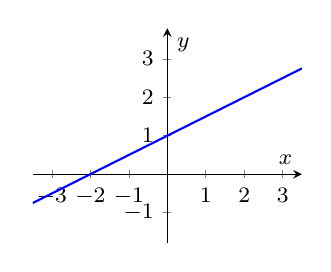
\begin{tikzpicture} 
\begin{axis}[footnotesize,font=\footnotesize,domain=-3.5:3.5
  ,axis equal, axis lines=middle,xlabel={$x$},ylabel={$y$}
  ] 
\addplot+[thick,no marks] {1+x/2};
\end{axis}
\end{tikzpicture}}
\begin{activity}[\temp]
Which one of the following is \emph{not} a valid vector equation for the line plotted to the right?
\actposs{\((-1,1/2)+(2,-1)t\)}
{\((2,2)+(1,1/2)t\)}
{\((0,1)+(2,1)t\)}
{\((-2,0)+(-4,-2)t\)}
\end{activity}
\endgroup



\begin{definition} \label{def:parlin}
A \bfidx{parametric equation} of a line is \(\xv=\pv+t\dv\) where \pv~is the \idx{position vector} of some point on the line,  the so-called \bfidx{direction vector}~\dv\ is parallel to the line (\(\dv\neq\ov\)), and the \idx{scalar} \bfidx{parameter}~\(t\) varies over all real values, to give all position vectors~\xv\ on the line.
\end{definition}

Beautifully, this definition applies for lines in any number of dimensions by using vectors with the corresponding number of components.

{%begingroup
\newcommand{\temp}[1]{%
\qview{37}{42} {%
\begin{tikzpicture} 
\begin{axis}[footnotesize,font=\footnotesize
  ,axis equal ,view={\q}{30}
  ,xlabel={$x$},ylabel={$y$},zlabel={$z$},label shift={-1.5ex}
  ] 
\addplot3[mark=*] coordinates {(0,0,0)} node[below] {$O$};
\addplot3[mark=*] coordinates {(-4,-3,3)} node[below] 
{\ifnum1=#1$P$\else\tiny$(-4,-3,3)$\fi};
\addplot3[mark=*] coordinates {(3,2,1)} node[above] 
{\ifnum1=#1$Q$\else\tiny$(3,2,1)$\fi};
\ifnum1=#1
\addplot3[red,thick,quiver={u=-4,v=-3,w=3},-stealth] coordinates {(0,0,0)};
\node[below] at (axis cs:-2,-1.5,1.5) {$\pv$};
\addplot3[red,thick,quiver={u=7,v=5,w=-2},-stealth] coordinates {(-4,-3,3)};
\node[above] at (axis cs:0.2,0,1.8) {$\dv$};
\fi
\addplot3[brown,samples=2,no marks,domain=-0.3:1.5] ({-4+7*\x},{-3+5*\x},{3-2*\x});
\end{axis}
\end{tikzpicture}}}
\begin{wrapfigure}[7]r{0pt}\temp0\end{wrapfigure}
\begin{example} 
Given that the line drawn to the right in space goes through points~\((-4,-3,3)\) and~\((3,2,1)\), find a \idx{parametric equation} of the line.
\vspace{3ex}
\begin{solution} 
Let's call the points~\((-4,-3,3)\) and~\((3,2,1)\) as \(P\) and~\(Q\), respectively, and as shown below.
First,  choose a point on the line, say~\(P\), and set its position vector \(\pv=\ovect{OP}=(-4,-3,3)=-4\iv-3\jv+3\kv\), as drawn.
Second, choose a direction vector to be, say, \(\dv=\ovect{PQ}=(3,2,1)-(-4,-3,3)=7\iv+5\jv-2\kv\), also drawn.
A parametric equation of the line is then \(\xv=\pv+t\dv\)\,, specifically
\begin{eqnarray*}
\xv&=&(-4\iv-3\jv+3\kv)+t(7\iv+5\jv-2\kv)
\\&=&(-4+7t)\iv+(-3+5t)\jv+(3-2t)\kv.
\end{eqnarray*}
\hfill\temp1 \aqed
\end{solution}
\end{example}
}%endgroup


\begin{example} 
Given the \idx{parametric equation} of a line in space is \(\sloppy\xv=(-4+2t,3-t,-1-4t)\), find the value of the parameter~\(t\) that gives each of the following points on the line: \((-1.6,1.8,-5.8)\), \((-3,2.5,-3)\), and \((-6,4,4)\).
\begin{solution} 
\begin{itemize}
\item For the point \((-1.6,1.8,-5.8)\) we need to find the parameter value~\(t\) such that \(-4+2t=-1.6\), \(3-t=1.8\), and \(-1-4t=-5.8\)\,.
The first of these requires \(t=(-1.6+4)/2=1.2\), the second requires \(t=3-1.8=1.2\), and the third requires \(t=(-1+5.8)/4=1.2\)\,.
All three agree that choosing parameter \(t=1.2\) gives the \text{required point.}

\item For the point \((-3,2.5,-3)\) we need to find the parameter value~\(t\) such that \(-4+2t=-3\), \(3-t=2.5\), and \(-1-4t=-3\)\,.
The first of these requires \(t=(-3+4)/2=0.5\), the second requires \(t=3-2.5=0.5\), and the third requires \(t=(-1+3)/4=0.5\)\,.
All three agree that choosing parameter \(t=0.5\) gives the \text{required point.}

\item For the point \((-6,4,4)\) we need to find the parameter value~\(t\) such that \(-4+2t=-6\), \(3-t=4\), and \(-1-4t=4\)\,.
The first of these requires \(t=(-6+4)/2=-1\), the second requires \(t=3-4=-1\), and the third requires \(t=(-1-4)/4=-1.25\)\,.
Since these three require different values of~\(t\), namely~\(-1\) and~\(-1.25\), it means that there is no single value of the parameter~\(t\) that gives the required point.
That is, the point~\((-6,4,4)\) cannot be on the line.
Consequently the task is impossible.%
\footnote{\cref{sec:asie} develops how to treat such inconsistent information in order to `best solve' such impossible tasks.}

\end{itemize}
\end{solution}
\end{example}






\subsection{Manipulation requires algebraic properties}
\label{sec:mrap}

\begin{quoted}{\idx{Descartes}}
It seems to be nothing other than that art which they call by the barbarous name of `algebra', if only it could be disentangled from the multiple numbers and inexplicable figures that overwhelm it \ldots
\end{quoted}

To unleash the power of algebra on vectors, we need to know the properties of vector operations.
Many of the following properties are familiar, as they directly correspond to familiar properties of arithmetic operations on scalars.
Moreover, the proofs show that the vector properties follow directly from the familiar properties of arithmetic operations \text{on scalars.}

\begin{example} 
Let vectors \(\uv=(1,2)\), \(\vv=(3,1)\), and \(\wv=(-2,3)\), and let scalars \(a=-\tfrac12\) and \(b=\tfrac52\).
Verify the following properties hold:
\begin{enumerate}
\item \(\uv+\vv=\vv+\uv\) \quad(\idx{commutative law});
\begin{solution} 
\(\uv+\vv=(1,2)+(3,1) =(1+3,2+1) =(4,3)\), whereas \(\vv+\uv =(3,1)+(1,2) =(3+1,1+2)=(4,3)\) is the same. 
\end{solution}

\item \((\uv+\vv)+\wv=\uv+(\vv+\wv)\) \quad(\idx{associative law});
\begin{solution} 
\((\uv+\vv)+\wv =(4,3)+(-2,3) =(2,6)\), whereas 
\(\uv+(\vv+\wv) =\uv+((3,1)+(-2,3)) =(1,2)+(1,4) =(2,6)\) is the same.
\end{solution}

\item \(\uv+\ov=\uv\);
\begin{solution} 
\(\uv+\ov=(1,2)+(0,0)=(1+0,2+0)=(1,2)=\uv\)\,. 
\end{solution}

\item \(\uv+(-\uv)=\ov\);
\begin{solution} 
Recall \(-\uv=(-1)\uv=(-1)(1,2)=(-1,-2)\), and so \(\uv+(-\uv) =(1,2)+(-1,-2)=(1-1,2-2)=(0,0)=\ov\)\,. 
\end{solution}

\item \(a(\uv+\vv)=a\uv+a\vv\)\quad(a \idx{distributive law});
\begin{solution} 
\(a(\uv+\vv)=-\tfrac12(4,3) =(-\tfrac12\cdot4,-\tfrac12\cdot3) =(-2,-\tfrac32)\), whereas \(a\uv+a\vv =-\tfrac12(1,2)+(-\tfrac12)(3,1) =(-\tfrac12,-1)+(-\tfrac32,-\tfrac12) =(-\tfrac12-\tfrac32,-1-\tfrac12) =(-2,-\tfrac32)\) which is the same.
\end{solution}

\item \((a+b)\uv=a\uv+b\uv\)\quad(a \idx{distributive law});
\begin{solution} 
\((a+b)\uv=(-\tfrac12+\tfrac52)(1,2) =2(1,2) =(2\cdot1,2\cdot2) =(2,4)\), whereas \(a\uv+b\uv = (-\tfrac12)(1,2)+\tfrac52(1,2) =(-\tfrac12,-1)+(\tfrac52,5) =(-\tfrac12+\tfrac52,-1+5) =(-2,4)\) which is the same.
\end{solution}

\item \((ab)\uv=a(b\uv)\);
\begin{solution} 
\((ab)\uv=(-\tfrac12\cdot52)(1,2)=(-\tfrac54)(1,2) =(-\tfrac54,-\tfrac52)\), whereas \(a(b\uv)=a(\tfrac52(1,2)) =(-\tfrac12)(\tfrac52,5) =(-\tfrac54,-\tfrac52)\) which is the same.
\end{solution}

\item \(1\uv=\uv\);
\begin{solution} 
\(1\uv=1(1,2)=(1\cdot1,1\cdot2)=(1,2)=\uv\)\,. 
\end{solution}

\item \(0\uv=\ov\);
\begin{solution} 
\(0\uv=0(1,2)=(0\cdot1,0\cdot2)=(0,0)=\ov\)\,. 
\end{solution}

\item \(|a\uv|=|a|\cdot|\uv|\).
\begin{solution} 
Now \(|a|=|-\tfrac12|=\tfrac12\), and the length \(|\uv|=\sqrt{1^2+2^2}=\sqrt5\) (\cref{def:veclen}).
Consequently, \(|a\uv| =|(-\tfrac12)(1,2)| =|(-\tfrac12,-1)| =\sqrt{(-\tfrac12)^2+(-1)^2} =\sqrt{\tfrac14+1} =\sqrt{\tfrac54} =\tfrac12\sqrt5=|a|\cdot|\uv|\) as required.
\end{solution}

\end{enumerate}
\end{example}


Now let's state and prove these properties in general.


\begin{theorem} \label{thm:vecops}
For all vectors~\uv, \vv, and~\wv\  with \(n\)~components (that is, in~\(\RR^n\)), and for all \idx{scalar}s~\(a\) and~\(b\),
the following properties hold:
\begin{enumerate}[ref=\ref{thm:vecops}(\alph*)]
\item\label[theorem]{thm:vecopsa} \(\uv+\vv=\vv+\uv\) \quad(\idx{commutative law});
\item\label[theorem]{thm:vecopsb} \((\uv+\vv)+\wv=\uv+(\vv+\wv)\) \quad(\idx{associative law});
\item\label[theorem]{thm:vecopsc} \(\uv+\ov=\ov+\uv=\uv\);
\item\label[theorem]{thm:vecopsd} \(\uv+(-\uv)=(-\uv)+\uv=\ov\);
\item\label[theorem]{thm:vecopse} \(a(\uv+\vv)=a\uv+a\vv\)\quad(a \idx{distributive law});
\item\label[theorem]{thm:vecopsf} \((a+b)\uv=a\uv+b\uv\)\quad(a \idx{distributive law});
\item\label[theorem]{thm:vecopsg} \((ab)\uv=a(b\uv)\);
\item\label[theorem]{thm:vecopsh} \(1\uv=\uv\);
\item\label[theorem]{thm:vecopsi} \(0\uv=\ov\);
\item\label[theorem]{thm:vecopsj} \(|a\uv|=|a|\cdot|\uv|\).
\end{enumerate}
\end{theorem}

\begin{proof} 
We prove \ref{thm:vecopsa}, and leave the proof of other properties as exercises.
The approach is to establish the properties of vector operations using the known properties of scalar operations.

\newcommand{\twov}[5]{%
  \pgfmathparse{#2*0.9+#4}\let\h\pgfmathresult
  \pgfmathparse{#3*0.9+#5}\let\v\pgfmathresult
  \addplot+[thick,quiver={u=#2,v=#3},-stealth,mark=empty] coordinates {(#4,#5)};
  \addplot+[forget plot,mark=empty] coordinates {(#2*1.05+#4,#3*1.05+#5)};
  \edef\tempa{\noexpand
  \node[above] at (axis cs:\h,\v) {$#1$};
  }\tempa }%
\newcommand{\temp}[5]{\begin{tikzpicture} 
\begin{axis}[footnotesize,font=\footnotesize
  ,axis equal, axis lines=none
%  ,title={$\uv+\vv=\vv+\uv$}
  ] 
  \node[below] at (axis cs:0,0) {$O$};
  \twov{\noexpand\uv}{#2}{#3}00
  \twov{\noexpand\vv}{#4}{#5}00
  \addplot[forget plot,red,thick,quiver={u=#4,v=#5},-stealth] coordinates {(#2,#3)};
  \addplot[forget plot,blue,thick,quiver={u=#2,v=#3},-stealth] coordinates {(#4,#5)};
  \twov{\noexpand\uv+\noexpand\vv=\noexpand\vv+\noexpand\uv\noexpand\hspace*{4em}}{#2+#4}{#3+#5}00
\end{axis}
\end{tikzpicture}}%
\begin{figbox}{\temp01231}%
Property~\ref{thm:vecopsa} is the commutativity of vector addition.
\cref{eg:vecadda} shows graphically how the equality \(\uv+\vv=\vv+\uv\) in just one case, and the margin here shows another case.
In general, let vectors \(\uv=(\hlist un)\) and \(\vv=(\hlist vn)\) then
\begin{align*}
&{\uv+\vv}
\\&=(\hlist un)+(\hlist vn)
\\&=(u_1+v_1,u_2+v_2,\ldots,u_n+v_n)
\quad(\text{by \cref{def:vecops}})
\\&=(v_1+u_1,v_2+u_2,\ldots,v_n+u_n)
\quad(\text{commutative scalar add})
\\&=(\hlist vn)+(\hlist un)
\quad(\text{by \cref{def:vecops}})
\\&=\vv+\uv\,.  
\end{align*}
\ \end{figbox}
\end{proof}



\begin{wrapfigure}r{0pt}
\def\ux{3}\def\uy{-1}\def\vx{2}\def\vy{2}\def\wx{-1}\def\wy{2}
\begin{tikzpicture} 
\begin{axis}[footnotesize,font=\footnotesize
  ,axis equal, axis lines=none, 
  ] 
\addplot[mark=*] coordinates {(0,0)} node[below] {$O$};
\addplot[blue,thick,quiver={u=\ux,v=\uy},-stealth] coordinates {(0,0)};
\pgfmathparse{\ux/2}\let\ha\pgfmathresult
\pgfmathparse{\uy/2}\let\va\pgfmathresult
\node[below] at (axis cs:\ha,\va) {$\uv$};
\addplot[blue,thick,quiver={u=\vx,v=\vy},-stealth] coordinates {(\ux,\uy)};
\pgfmathparse{\ux+\vx/2}\let\hb\pgfmathresult
\pgfmathparse{\uy+\vy/2}\let\vb\pgfmathresult
\node[below] at (axis cs:\hb,\vb) {$\vv$};
\addplot[blue,thick,quiver={u=\wx,v=\wy},-stealth] coordinates {(\ux+\vx,\uy+\vy)};
\pgfmathparse{\ux+\vx+\wx/2}\let\hc\pgfmathresult
\pgfmathparse{\uy+\vy+\wy/2}\let\vc\pgfmathresult
\node[below] at (axis cs:\hc,\vc) {$\wv$};
%
\addplot[red,thick,quiver={u=\ux+\vx,v=\uy+\vy},-stealth] coordinates {(0,0)};
\addplot[red,thick,quiver={u=\vx+\wx,v=\vy+\wy},-stealth] coordinates {(\ux,\uy)};
\addplot[brown,thick,quiver={u=\ux+\vx+\wx,v=\uy+\vy+\wy},-stealth] coordinates {(0,0)};
\end{axis}
\end{tikzpicture}
\qquad
\begin{tikzpicture} 
\begin{axis}[footnotesize,font=\footnotesize
  ,axis equal, axis lines=none, 
  ] 
\addplot[mark=*] coordinates {(0,0)} node[below] {$O$};
\addplot[blue,thick,quiver={u=\ux,v=\uy},-stealth] coordinates {(0,0)};
\pgfmathparse{\ux/2}\let\ha\pgfmathresult
\pgfmathparse{\uy/2}\let\va\pgfmathresult
\node[below] at (axis cs:\ha,\va) {$\uv$};
\addplot[blue,thick,quiver={u=\vx,v=\vy},-stealth] coordinates {(\ux,\uy)};
\pgfmathparse{\ux+\vx/2}\let\hb\pgfmathresult
\pgfmathparse{\uy+\vy/2}\let\vb\pgfmathresult
\node[below] at (axis cs:\hb,\vb) {$\vv$};
\addplot[blue,thick,quiver={u=\wx,v=\wy},-stealth] coordinates {(\ux+\vx,\uy+\vy)};
\pgfmathparse{\ux+\vx+\wx/2}\let\hc\pgfmathresult
\pgfmathparse{\uy+\vy+\wy/2}\let\vc\pgfmathresult
\node[right] at (axis cs:\hc,\vc) {$\wv$};
%
\addplot[red,thick,quiver={u=\ux+\vx,v=\uy+\vy},-stealth] coordinates {(0,0)};
\addplot[red,thick,quiver={u=\vx+\wx,v=\vy+\wy},-stealth] coordinates {(0,0)};
\addplot[brown,thick,quiver={u=\ux+\vx+\wx,v=\uy+\vy+\wy},-stealth] coordinates {(0,0)};
%
\addplot[blue,thick,quiver={u=\vx,v=\vy},-stealth] coordinates {(0,0)};
\pgfmathparse{\vx/2}\let\hd\pgfmathresult
\pgfmathparse{\vy/2}\let\vd\pgfmathresult
\node[above] at (axis cs:\hd,\vd) {$\vv$};
\addplot[blue,thick,quiver={u=\wx,v=\wy},-stealth] coordinates {(\vx,\vy)};
\pgfmathparse{\vx+\wx/2}\let\he\pgfmathresult
\pgfmathparse{\vy+\wy/2}\let\ve\pgfmathresult
\node[right] at (axis cs:\he,\ve) {$\wv$};
\addplot[blue,thick,quiver={u=\ux,v=\uy},-stealth] coordinates {(\wx+\vx,\wy+\vy)};
\pgfmathparse{\ux/2+\vx+\wx}\let\hf\pgfmathresult
\pgfmathparse{\uy/2+\vy+\wy}\let\vf\pgfmathresult
\node[above] at (axis cs:\hf,\vf) {$\uv$};
\end{axis}
\end{tikzpicture}
\end{wrapfigure}
\begin{example} 
Which of these two diagrams best illustrates the \idx{associative law}~\ref{thm:vecopsb}?  Give reasons.
\begin{solution} 
The left diagram.

\begin{itemize}
\item In the left diagram, the two red vectors represent \(\uv+\vv\) (left) and \(\vv+\wv\) (right).
Thus the left-red followed by the blue~\wv\ represents \((\uv+\vv)+\wv\), whereas the \uv\ followed by the right-red represents \(\uv+(\vv+\wv)\).
The brown vector shows that they are equal: \((\uv+\vv)+\wv=\uv+(\vv+\wv)\).
\fixwrapitem
\item The right-hand of the two diagrams invokes the commutative law as well.
The top-left part of the diagram shows \((\vv+\wv)+\uv\), whereas the bottom-right part shows \((\uv+\vv)+\wv\).
That these are equal, the brown vector, requires both the commutative and associative laws.
\aqed
\end{itemize}
\end{solution}
\end{example}


We frequently use the algebraic properties of \cref{thm:vecops} in rearranging and solving vector equations. 

\begin{example} 
Find the vector~\xv\ such that \(3\xv-2\uv=6\vv\)\,.
\begin{solution} 
Using \cref{thm:vecops}, all the following equations are equivalent:
\begin{eqnarray*}
3\xv-2\uv&=&6\vv
;\\
(3\xv-2\uv)+2\uv&=&6\vv+2\uv
\quad(\text{add \(2\uv\) to both sides});\\
3\xv+(-2\uv+2\uv)&=&6\vv+2\uv
\quad\text{(by \ref{thm:vecopsb}, associativity);}\\
3\xv+\ov&=&6\vv+2\uv
\quad(\text{by \ref{thm:vecopsd}});\\
3\xv&=&6\vv+2\uv
\quad(\text{by \ref{thm:vecopsc}});\\
\tfrac13(3\xv)&=&\tfrac13(6\vv+2\uv)
\quad(\text{multiply both sides by }\tfrac13);\\
\tfrac13(3\xv)&=&\tfrac13(6\vv)+\tfrac13(2\uv)
\quad\text{(by \ref{thm:vecopse}, distributivity);}\\
(\tfrac13\cdot3)\xv&=&(\tfrac13\cdot6)\vv+(\tfrac13\cdot2)\uv
\quad(\text{by \ref{thm:vecopsg}});\\
1\xv&=&2\vv+\tfrac23\uv
\quad(\text{by scalar operations});\\
\xv&=&2\vv+\tfrac23\uv
\quad(\text{by \ref{thm:vecopsh}}).
\end{eqnarray*}
Generally we do not write down all such details.
Generally the following shorter derivation is acceptable.
The following are equivalent:
\begin{eqnarray*}
3\xv-2\uv&=&6\vv
;\\
3\xv&=&6\vv+2\uv
\quad(\text{adding \(2\uv\) to both sides});\\
\xv&=&2\vv+\tfrac23\uv
\quad(\text{dividing both sides by }3).
\end{eqnarray*}
But exercises and examples in this section sometimes explicitly require full details and justification.
\end{solution}
\end{example}




\begin{OmitV1}
\begin{example} 
Rearrange \(3\xv-\av=2(\av+\xv)\) to write vector~\xv\ in terms of~\av: give excruciating detail of the justification using \cref{thm:vecops}.
\begin{solution} 
Using \cref{thm:vecops}, the following statements are equivalent:
\begin{eqnarray*}
3\xv-\av&=&2(\av+\xv)
\\3\xv-\av&=&2\av+2\xv
\quad\text{(by \ref{thm:vecopse}, distributivity);}
\\(3\xv-\av)+\av&=&(2\av+2\xv)+\av
\quad(\text{adding \av\ to both sides});
\\3\xv+(-\av+\av)&=&2\av+(2\xv+\av)
\quad\text{(by \ref{thm:vecopsb}, associativity);}
\\3\xv+\ov&=&2\av+(\av+2\xv)
\quad\text{(by \ref{thm:vecopsd} \& \ref{thm:vecopsa});}
\\3\xv&=&(2\av+\av)+2\xv
\quad\text{(by \ref{thm:vecopsc} \& \ref{thm:vecopsb});}
\\3\xv&=&(2\av+1\av)+2\xv
\quad(\text{by \ref{thm:vecopsh}});
\\3\xv&=&(2+1)\av+2\xv
\quad\text{(by \ref{thm:vecopsf}, distributivity);}
\\3\xv+(-2)\xv&=&3\av+2\xv+(-2)\xv
\quad(\text{sub.\ \(2\xv\) from both sides});
\\(3+(-2))\xv&=&3\av+(2+(-2))\xv
\quad\text{(by \ref{thm:vecopsf}, distributivity);}
\\1\xv&=&3\av+0\xv
\quad(\text{by scalar arithmetic});
\\\xv&=&3\av+\ov
\quad\text{(by \ref{thm:vecopsh} \& \ref{thm:vecopsi});}
\\\xv&=&3\av
\quad(\text{by \ref{thm:vecopsc}}).
\end{eqnarray*}
If the question had not requested full details, then the following would be enough.
The following statements are equivalent:
\begin{eqnarray*}
3\xv-\av&=&2(\av+\xv)
\quad(\text{distribute the mupltiplication})
\\3\xv&=&2\av+2\xv+\av
\quad(\text{adding \av\ to both sides});
\\\xv&=&3\av
\quad(\text{subtracting \(2\xv\) from both sides}).
\end{eqnarray*}
\end{solution}
\end{example}
\end{OmitV1}








\sectionExercises
\begin{exercise}  
For each of the pairs of vectors~\uv\ and~\vv\ shown below, draw the vectors \(\uv+\vv\), \(\vv+\uv\), \(\uv-\vv\), \(\vv-\uv\), \(\tfrac12\uv\), and~\(-\vv\).
\begin{Parts}
\item\vecops0{-1.}{3.4}{-3.2}{-0.1}
\item\vecops0{0.5}{1.9}{2.9}{-3.6}
\item\vecops0{-2.3}{-1.7}{0.3}{-1.5}
\item\vecops0{-3.2}{-1.6}{5.1}{-1.6}
\end{Parts}
\end{exercise}


\begin{exercise}  
For each of the following pairs of vectors shown below, use a ruler (or other measuring stick) to directly measure the \idx{distance} between the pair of vectors.
\newcommand{\mytmp}[4]{\begin{tikzpicture}
\begin{axis}[footnotesize,font=\footnotesize
,axis equal,axis lines=middle]
\twovec{\noexpand\vec a}{#1}{#2}00
\twovec{\noexpand\vec b}{#3}{#4}00
\end{axis}
\end{tikzpicture}}
\begin{Parts}
\item \mytmp{-2.6}{-1.8}{-0.3}{3.6}
\answer{\(5.9\)}
\item \mytmp{-2.3}{0.3}{-2.2}{-1.}
\answer{\(1.3\)}
\begin{OmitV1}
\item \mytmp{-2.4}{0.4}{-4.5}{-0.3}
\answer{\(2.2\)}
\item \mytmp{2.2}{9.7}{-1.4}{4.3}
\answer{\(6.5\)}
\end{OmitV1}
\item \mytmp{-2.4}{-1.6}{2.}{0.6}
\answer{\(4.9\)}
\item \mytmp{0.5}{2.5}{1.4}{-0.9}
\answer{\(3.5\)}
\end{Parts}
\end{exercise}


\begin{exercise}  
For each of the following groups of vectors, use the \idx{distance} between vectors to find which pair in the group are closest to each other, and which pair in the group are furthest from each other. 
\begin{enumerate} \sloppy
\item \(\uv=(-5,0,3)\), \(\vv=(1,-6,10)\), \(\wv=(-4,4,11)\)
\answer{\uv~and~\wv\ are closest; \vv~and~\wv\ are furthest.}

\begin{OmitV1}
\item \(\uv=(2,2,-1)\), \(\vv=(3,6,-9)\), \(\wv=(1,-2,-9)\)
\answer{\uv~and~\wv\ are closest; both the other pairs are equal furthest.}

\item \(\uv=(1,1,-3)\), \(\vv=(7,7,-10)\), \(\wv=(-1,4,-9)\)
\answer{\uv~and~\wv\ are closest; \vv~and~\uv\ are furthest.}
\end{OmitV1}

\item \(\uv=3\iv\), \(\vv=4\iv-2\jv+2\kv\), \(\wv=4\iv+2\jv+2\kv\)
\answer{\vv~and~\wv\ are furthest; both the other pairs are equal closest.}

\item \(\uv=(-5,3,5,6)\), \(\vv=(-6,1,3,10)\), \(\wv=(-4,6,2,15)\)
\answer{\uv~and\vv\ are closest; \uv~and~\wv\ are furthest.}

\begin{OmitV1}
\item \(\uv=(-4,-1,-1,2)\), \(\vv=( -5,-2,-2,1)\), \(\wv=(-3,-2,-2,1)\)
\answer{all pairs are the same distance apart.}

\item \(\uv=5\ev_1+\ev_3+5\ev_4\), \(\vv=6\ev_1-2\ev_2+3\ev_3+\ev_4\), \(\wv=7\ev_1-2\ev_2-3\ev_3\)
\answer{\uv~and~\vv\ are closest; \uv~and~\wv\ are furthest.}
\end{OmitV1}%

\item \(\uv= 2\ev_1+4\ev_2-\ev_3+5\ev_4\), \(\vv=-2\ev_1+8\ev_2-6\ev_3-3\ev_4\), \(\wv=-6\ev_3+11\ev_4\)
\answer{\uv~and~\wv\ are closest; \vv~and~\wv\ are furthest.}

\end{enumerate}
%\begin{comment}
%\begin{verbatim}
%xx=[1    2    2    3
%    2    3    6    7
%    4    4    7    9
%    6    6    7   11
%    1    4    8    9
%    2    6    9   11]
%xx=[1    1    1    1    2
%    1    2    2    4    5
%    1    4    4    4    7
%    1    1    3    5    6
%    2    2    4    5    7
%    2    4    5    6    9
%    1    5    5    7   10
%    1    1    7    7   10
%    2    2    3    8    9
%    4    4    5    8   11
%    2    2    7    8   11
%    4    5    8    8   13
%    1    3    3    9   10
%    4    6    6    9   13
%    4    8    8    9   15
%    3    5    9    9   14]
%n=size(xx,2)-1
%for i=1:8
%u=round(randn(1,n)*3)
%v=u+sign(randn(1,n)).*xx(ceil(rand*size(xx,1)),1:n)
%w=u+sign(randn(1,n)).*xx(ceil(rand*size(xx,1)),1:n)
%ds=[norm(v-w) norm(u-w) norm(u-v) ]
%end
%\end{verbatim}
%\end{comment}
\end{exercise}





\begin{exercise}  
Find a \idx{parametric equation} of the line through the given pairs of points.
\begin{Parts}
\item \((-11,0,3)\),
   \((-3,-2,2)\)
\answer{One possibility is \(\xv=(-11+8t,-2t,3-t)\)}

\item \((-4,1,-2)\),
   \((3,-5,5)\)
\answer{One possibility is \(\xv=(-4+7t)\iv+(1-6t)\jv+(-2+7t)\kv\)}

\begin{OmitV1}
\item \((2.4,5.5,-3.9)\),
   \((1.5,-5.4,-0.5)\)
\answer{One possibility is \(\xv=(2.4-0.9t,5.5-10.9t,-3.9+3.4t)\)}

\item \((0.2,-7.2,-4.6,-2.8)\),
   \((3.3,-1.1,-0.4,-0.3)\)
\answer{One possibility is \(\xv=(0.2+3.1t)\ev_1 +(-7.2+6.1t)\ev_2 +(-4.6+4.2t)\ev_3+(-2.8+2.5t)\ev_4\)}
\end{OmitV1}

\item \((2.2,5.8,4,3,2)\),
   \((-1.1,2.2,-2.4,-3.2,0.9)\)
\answer{One possibility is \(\xv=(2.2-3.3t,5.8-3.6t,4-6.4t,3-6.2t,2-1.1t)\)}

\item \((1.8,-3.1,-1,-1.3,-3.3)\),
   \((-1.4,0.8,-2.6,3.1,-0.8)\)
\answer{One possibility is \(\xv=(1.8-3.2t)\ev_1 +(-3.1+3.9t)\ev_2 -(1+1.6t)\ev_3 +(-1.3+4.1t)\ev_4 +(-3.3+2.5t)\ev_5\)}

\end{Parts}
\end{exercise}



\begin{exercise}  
Verify the algebraic properties of \cref{thm:vecops} for each of the following sets of vectors and scalars.
\begin{enumerate}
\item \(\uv=2.4\iv-0.3\jv\), \(\vv=-1.9\iv+0.5\jv\), \(\wv=-3.5\iv-1.8\jv\), \(a=0.4\), and \(b=1.4\).
\begin{OmitV1}
\item \(\uv=(1/3,14/3)\), \(\vv=(4,4)\), \(\wv=(2/3,-10/3)\), \(a=-2/3\), and \(b=-1\).
\end{OmitV1}
\item \(\uv=-\frac12\jv+\frac32\kv\), \(\vv=2\iv-\jv\), \(\wv=2\iv-\kv\), \(a=-3\), and \(b=\frac12\).
\item \(\uv=(2,1,4,-2)\), \(\vv=(-3,-2,0,-1)\), \(\wv=(-6,5,4,2)\), \(a=-4\), and \(b=3\).
\end{enumerate}
\end{exercise}




\begin{exercise}  
Prove in detail some algebraic properties chosen from \cref{thm:vecopsb}--\ref{thm:vecopsj} on vector addition and \idx{scalar multiplication}.
\end{exercise}




\begin{exercise}  
For each of the following vector equations, rearrange the equation to get vector~\xv\ in terms of the other vectors.  Give excruciating detail of the justification, using \cref{thm:vecops}.
\begin{Parts}
\item \(\xv+\av=\ov\).
\item \(2\xv-\bv=3\bv\).
\item \(3(\xv+\av)=\xv+(\av-2\xv)\).
\item \(-4\bv=\xv+3(\av-\xv)\).
\end{Parts}
\end{exercise}




\begin{exercise}  
In a few sentences, answer\slash discuss each of the following.
\begin{enumerate}
\item What empowers us to write every vector in terms of the standard unit vectors?

\item We use the distance~\(|\uv-\vv|\) to measure how close the two vectors are to each other.  Invent an alternative way to measure closeness of two vectors, and comment on why your invented alternative measures closeness.
% Could be any in q-norm family, or a weighted q-norm, but not the angle between vectors.

\item What is it about the parametric equation of a line that means it does indeed describe a line in space?

\item Comment on why many of the properties of vector operations (\cref{thm:vecops}) appear the same as those for operations with real numbers. 


\end{enumerate}
\end{exercise}





\begin{comment}%{ED498555.pdf}
why, what caused X?
how did X occur?
what-if? what-if-not?
how does X compare with Y?
what is the evidence for X?
why is X important?
\end{comment}

%!TEX root = ../larxxia.tex

\section{The dot product determines angles and lengths}
\label{sec:dpdal}
\secttoc

\index{dot product|(}
\index{length|(}
\index{angle|(}

The previous \autoref{sec:asv} discussed how to add, subtract and stretch vectors.
Question: can we multiply two vectors?
The answer is that `vector multiplication' has major differences to the multiplication of scalar numbers.
There are at least four ways of multiplying vectors together: each way useful in appropriate circumstances.
\begin{aside}
Often the angle between vectors is denoted by the Greek letter theta,~\(\theta\).
\end{aside}%
This section introduces one such multiplication, the so-called dot product of two vectors that, among other attributes, gives a valuable way to determine the angle between two vectors.

\begin{example} \label{eg:ezyang}
Consider the two vectors \(\uv=(7,-1)\) and \(\vv=(2,5)\) plotted in the margin.
\def\vecopsHook{\node[above] at (axis cs:0,0) {$\qquad\theta$};}
\marginpar{\vecops07{-1}25}
What is the angle~\(\theta\) between the two vectors?
\begin{solution} 
Form a triangle with the vector \(\uv-\vv=(5,-6)\) going from the tip of~\vv\ to the tip of~\uv, as shown in the margin.
\marginpar{\vecops37{-1}25}%
The sides of the triangles are of length \(|\uv|=\sqrt{7^2+(-1)^2}=\sqrt{50}=5\sqrt2\), \(|\vv|=\sqrt{2^2+5^2}=\sqrt{29}\), and \(|\uv-\vv|=\sqrt{5^2+(-6)^2}=\sqrt{61}\).
By the \idx{cosine rule} for triangles
\begin{equation*}
|\uv-\vv|^2=|\uv|^2+|\vv|^2-2|\uv||\vv|\cos\theta \,.
\end{equation*}
Here this rule rearranges to
\begin{eqnarray*}
|\uv||\vv|\cos\theta
&=&\tfrac12(|\uv|^2+|\vv|^2-|\uv-\vv|^2)
\\&=&\tfrac12(50+29-61)
\\&=&9\,.
\end{eqnarray*}
\begin{aside}
Recall that multiplication by~\(180/\pi\) converts an angle from radians to degrees (\(1.3322\cdot180/\pi=76.33^\circ\)).
\end{aside}%
Dividing by the product of the lengths then gives \(\cos\theta=9/(5\sqrt{58})=0.2364\) 
so the angle \(\theta =\arccos(0.2364) =1.3322 =76.33^\circ\) as is reasonable from the plots.
\end{solution}
\end{example}

The interest in this \autoref{eg:ezyang} is the number nine on the right-hand side of \(|\uv||\vv|\cos\theta=9\)\,.  
The reason is that~\(9\) just happens to be~\(14-5\), which in turn just happens to be \(7\cdot2+(-1)\cdot5\), and it is no coincidence that this expression is the same as \(u_1v_1+u_2v_2\) in terms of vector components \(\uv=(u_1,u_2)=(7,-1)\) and \(\vv=(v_1,v_2)=(2,5)\).
Repeat this example for many pairs of vectors~\uv\ and~\vv\ to find that always \(|\uv||\vv|\cos\theta=u_1v_1+u_2v_2\) (\autoref{ex:ezyang}).
This equality suggests that the sum of products of corresponding components of~\uv\ and~\vv\ is closely connected to the angle between the vectors.


\begin{definition} \label{def:dotprod}
For every two vectors in~\(\RR^n\), $\uv=(\hlist un)$ and $\vv=(\hlist vn)$,
define the \bfidx{dot product} (or \bfidx{inner product}), denoted by a dot between the two vectors, as the \idx{scalar}
\begin{equation*}
\uv\cdot \vv:= \lincomb uvn\,.
\end{equation*}
\end{definition}

The dot product of two vectors gives a scalar result, a number, not a vector result.

When writing the vector dot product, the dot between the two vectors is essential.
We sometimes also denote the scalar product by such a dot (to clarify a product) and sometimes omit the dot between the scalars, for example \(a\cdot b=ab\) for scalars. 
But for the vector dot product the dot must not be omitted: `\(\uv\vv\)' is meaningless.


\begin{example} 
Compute the dot product between the following pairs of vectors.
\begin{enumerate}
\item \(\uv=(-2,5,-2)\), \(\vv=(3,3,-2)\)
\begin{solution} 
\(\uv\cdot\vv=(-2)3+5\cdot3+(-2)(-2)=13\)\,. 
Alternatively, \(\vv\cdot\uv=3(-2)+3\cdot5+(-2)(-2)=13\)\,.
That these give the same result is a consequence of a general commutative law, \autoref{thm:dotopsa}, and so in the following we compute the dot product only one way around.
\end{solution}

\item \(\uv=(1,-3,0)\), \(\vv=(1,2)\)
\begin{solution} 
There is no answer: a dot product cannot be computed here as the two vectors are of different sizes. 
\end{solution}

\begin{reduce}
\item \(\av=(-7,3,0,2,2)\), \(\bv=(-3,4,-4,2,0)\)
\begin{solution} 
\(\av\cdot\bv=(-7)(-3)+3\cdot4+0(-4)+2\cdot2+2\cdot0=37\). 
\end{solution}
\end{reduce}

\item \(\pv=(-0.1,-2.5,-3.3,0.2)\), \(\qv=(-1.6,1.1,-3.4,2.2)\)
\begin{solution} 
\(\pv\cdot\qv=(-0.1)(-1.6)+(-2.5)1.1+(-3.3)(-3.4)+0.2\cdot2.2=9.07\).
\end{solution}
\end{enumerate}
\end{example}



\begin{activity}
What is the dot product of the two vectors \(\uv=2\iv-\jv\) and \(\vv=3\iv+4\jv\)\,?
\actposs[4]{\(2\)}{\(5\)}{\(8\)}{\(10\)}
\end{activity}





\begin{theorem} \label{thm:anglev}
For every two nonzero vectors~\uv\ and~\vv\ in~\(\RR^n\),  
the \bfidx{angle}~\(\theta\) between the vectors is determined by 
\begin{equation*}
\cos\theta=\frac{\uv\cdot\vv}{|\uv||\vv|}\,,
\quad 0\leq\theta\leq\pi
\quad (0\leq\theta\leq180^\circ).
\end{equation*}
\end{theorem}

\begin{wrapfigure}{r}{0pt} 
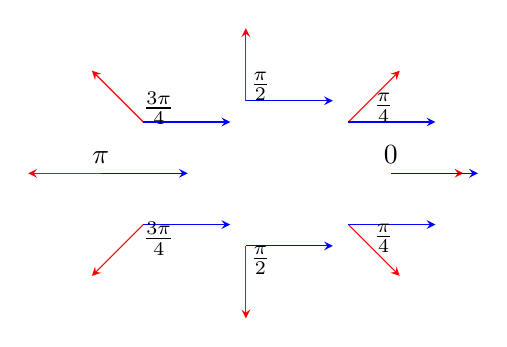
\begin{tikzpicture} 
\begin{axis}[axis equal image,hide axis,domain=-135:180]
    \addplot[quiver={u=x,v=2*y,scale arrows=0.5},
        red,-stealth,samples=8] ({cos(x)},{sin(x)/2});
    \addplot[quiver={u=1,v=0,scale arrows=0.6},
        blue,-stealth,samples=8] ({cos(x)},{sin(x)/2});
    \node at (axis cs:0.95,0.45) {$\frac\pi4$};
    \node at (axis cs:0.95,-0.45) {$\frac\pi4$};
    \node at (axis cs:0.1,0.6) {$\frac\pi2$};
    \node at (axis cs:0.1,-0.6) {$\frac\pi2$};
    \node at (axis cs:-0.6,0.45) {$\frac{3\pi}4$};
    \node at (axis cs:-0.6,-0.45) {$\frac{3\pi}4$};
    \node[above] at (axis cs:-1,0) {$\pi$};
    \node[above] at (axis cs:1,0) {$0$};
\end{axis}
\end{tikzpicture}
\end{wrapfigure}
This picture illustrates the range of angles between two vectors: when they point in the same direction the angle is zero; when they are at \idx{right-angles} to each other the angle is~\(\pi/2\), or equivalently~\(90^\circ\); when they point in opposite directions the angle is~\(\pi\), or equivalently~\(180^\circ\).
Let's prove this theorem after some examples.



\begin{example} 
Determine the \idx{angle} between the following pairs of vectors.
\begin{enumerate}
\item \((4,3)\) and \((5,12)\)
\begin{solution} 
These vectors (shown in the margin) 
\marginpar{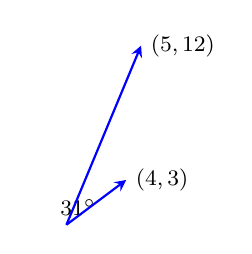
\begin{tikzpicture} 
\begin{axis}[footnotesize,font=\footnotesize
  ,axis equal, axis lines=none
  ] 
  \node[above] at (axis cs:0,0) {$\quad31^\circ$};
  \addplot[blue,thick,quiver={u=4,v=3},-stealth,mark=empty] coordinates {(0,0)};
  \node[right] at (axis cs:4,3) {$(4,3)$};
  \addplot[blue,thick,quiver={u=5,v=12},-stealth,mark=empty] coordinates {(0,0)};
  \node[right] at (axis cs:5,12) {$(5,12)$};
\end{axis}
\end{tikzpicture}}%
have length \(\sqrt{4^2+3^2}=\sqrt{25}=5\) and \(\sqrt{5^2+12^2}=\sqrt{169}=13\), respectively.
Their dot product  \((4,3)\cdot(5,12)=20+36=56\).
Hence \(\cos\theta =56/(5\cdot13) =0.8615\) and so angle \(\theta =\arccos(0.8615) =0.5325 =30.51^\circ\).
\end{solution}


\item \((3,1)\) and \((-2,1)\)
\begin{solution} 
These vectors (shown in the margin) 
\marginpar{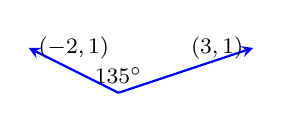
\begin{tikzpicture} 
\begin{axis}[footnotesize,font=\footnotesize
  ,axis equal, axis lines=none
  ] 
  \node[above] at (axis cs:0,0) {$135^\circ$};
  \addplot[blue,thick,quiver={u=3,v=1},-stealth,mark=empty] coordinates {(0,0)};
  \node[left] at (axis cs:3,1) {$(3,1)$};
  \addplot[blue,thick,quiver={u=-2,v=1},-stealth,mark=empty] coordinates {(0,0)};
  \node[right] at (axis cs:-2,1) {$(-2,1)$};
\end{axis}
\end{tikzpicture}}%
have length \(\sqrt{3^2+1^2}=\sqrt{10}\) and \(\sqrt{(-2)^2+1^2}=\sqrt{5}\), respectively.
Their dot product  \((3,1)\cdot(-2,1)=-6+1=-5\).
Hence \(\cos\theta =-5/(\sqrt{10}\cdot\sqrt5) =-1/\sqrt2 =-0.7071\) and so angle \(\theta =\arccos(-1/\sqrt2) =2.3562 =\frac34\pi =135^\circ\) (\autoref{tbl:cosines}).
\end{solution}



\begin{reduce}
\item \((4,-2)\) and \((-1,-2)\)
\begin{solution} 
These vectors (shown in the margin) 
\marginpar{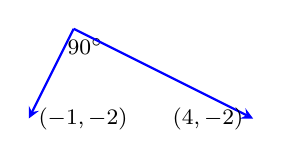
\begin{tikzpicture} 
\begin{axis}[footnotesize,font=\footnotesize
  ,axis equal, axis lines=none
  ] 
  \node[below] at (axis cs:0,0) {$\quad90^\circ$};
  \addplot[blue,thick,quiver={u=4,v=-2},-stealth,mark=empty] coordinates {(0,0)};
  \node[left] at (axis cs:4,-2) {$(4,-2)$};
  \addplot[blue,thick,quiver={u=-1,v=-2},-stealth,mark=empty] coordinates {(0,0)};
  \node[right] at (axis cs:-1,-2) {$(-1,-2)$};
\end{axis}
\end{tikzpicture}}%
have length \(\sqrt{4^2+(-2)^2}=\sqrt{20}=2\sqrt5\) and \(\sqrt{(-1)^2+(-2)^2}=\sqrt{5}\), respectively.
Their dot product  \((4,-2)\cdot(-1,-2)=-4+4=0\).
Hence \(\cos\theta =0/(2\sqrt{5}\cdot\sqrt5) =0\) and so angle \(\theta=\frac12\pi=90^\circ\) (\autoref{tbl:cosines}).
\end{solution}
\end{reduce}

\end{enumerate}
\end{example}



\begin{activity}
What is the angle between the two vectors \((1,\sqrt3)\) and \((\sqrt3,1)\)?
\actposs[4]{\(30^\circ\)}{\(60^\circ\)}{\(64.34^\circ\)}{\(77.50^\circ\)}
\end{activity}




\begin{table}
\caption{when a \idx{cosine} is one of these tabulated special values, then we know the corresponding \idx{angle} exactly.  
In other cases we usually use a calculator (\texttt{arccos} or \(\texttt{cos}^{-1}\)) or computer (\texttt{acos()}) to compute the angle numerically.}
\label{tbl:cosines}
\index{arc-cos}\index{acos()@\texttt{acos()}}%
\begin{equation*}\def\arraystretch{1.1}
\begin{array}{crcr@.l}
\hline
\theta&\theta&\cos\theta&\multicolumn2c{\cos\theta}
\\\hline
0&0^\circ&1&1
\\\pi/6&30^\circ&{\sqrt3}/2&0&8660
\\\pi/4&45^\circ&1/{\sqrt2}&0&7071
\\\pi/3&60^\circ&1/2&0&5
\\\pi/2&90^\circ&0&0
\\{2\pi}/3&120^\circ&-1/2&-0&5
\\{3\pi}/4&135^\circ&-1/{\sqrt2}&-0&7071
\\{5\pi}/6&150^\circ&-{\sqrt3}/2&-0&8660
\\\pi&180^\circ&-1&-1
\\\hline
\end{array}
\end{equation*}
\end{table}




\begin{example} 
\index{bond angles}
In \idx{chemistry} one computes the angles between bonds in molecules and crystals.  
In engineering one needs the angles between beams and struts in complex structures.
The \idx{dot product} determines such \idx{angle}s.
\needspace{8\baselineskip}
\begin{enumerate}
\item Consider the cube drawn in stereo below, and compute the angle between the diagonals on two adjacent faces.
\begin{center}
\qview{50}{55} {\begin{tikzpicture} 
\begin{axis}[footnotesize,font=\footnotesize,view={\q}{30}
  ,axis equal, axis lines=box, height=5cm
  ] 
  \node[below] at (axis cs:0,0,0) {$O$};
  \addplot3[blue,mark=empty] coordinates {
  (0,0,0)(1,0,0)(1,1,0)(0,1,0)(0,0,0)(0,0,1)(1,0,1)(1,0,0)
  (1,0,1)(1,1,1)(1,1,0)(1,1,1)(0,1,1)(0,1,0)(0,1,1)(0,0,1)};
  \addplot3[red,thick,quiver={u=1,v=1,w=0},-stealth] coordinates {(0,0,0)};
  \addplot3[red,thick,quiver={u=0,v=1,w=1},-stealth] coordinates {(0,0,0)};
  \node[above] at (axis cs:0,0,0) {$\qquad\theta$};
\end{axis}
\end{tikzpicture}}
\end{center}
\begin{solution} 
Draw two vectors along adjacent diagonals: the above pair of vectors are \((1,1,0)\) and \((0,1,1)\).
They both have the same length as \(|(1,1,0)|=\sqrt{1^2+1^2+0^2}=\sqrt2\) and \(|(0,1,1)|=\sqrt{0^2+1^2+1^2}=\sqrt2\)\,.
The dot product is \((1,1,0)\cdot(0,1,1)=0+1+0=1\)\,.
Hence the cosine \(\cos\theta=1/(\sqrt2\cdot\sqrt2)=1/2\)\,.
\autoref{tbl:cosines} gives the angle \(\theta=\frac\pi3=60^\circ\).
\end{solution}

\begin{reduce}
\needspace{8\baselineskip}
\item Consider the cube drawn in stereo below: what is the angle between a diagonal on a face and a diagonal of the cube?
\begin{center}
\qview{50}{55} {
\begin{tikzpicture} 
\begin{axis}[footnotesize,font=\footnotesize,view={\q}{30}
  ,axis equal, axis lines=box, height=5cm
  ] 
  \node[below] at (axis cs:0,0,0) {$O$};
  \addplot3[blue,mark=empty] coordinates {
  (0,0,0)(1,0,0)(1,1,0)(0,1,0)(0,0,0)(0,0,1)(1,0,1)(1,0,0)
  (1,0,1)(1,1,1)(1,1,0)(1,1,1)(0,1,1)(0,1,0)(0,1,1)(0,0,1)};
  \addplot3[red,thick,quiver={u=1,v=1,w=0},-stealth] coordinates {(0,0,0)};
  \addplot3[red,thick,quiver={u=1,v=1,w=1},-stealth] coordinates {(0,0,0)};
  \node[above] at (axis cs:0.3,0.3,0) {$\theta$};
\end{axis}
\end{tikzpicture}}
\end{center}
\begin{solution} 
Draw two vectors along the diagonals: the above pair of vectors are \((1,1,0)\) and \((1,1,1)\).
The face-diagonal has length \(|(1,1,0)|=\sqrt{1^2+1^2+0^2}=\sqrt2\) whereas the cube diagonal has length \(|(1,1,1)|=\sqrt{1^2+1^2+1^2}=\sqrt3\)\,.
The dot product is \((1,1,0)\cdot(1,1,1)=1+1+0=2\)\,.
Hence  \(\cos\theta=2/(\sqrt2\cdot\sqrt3)=\sqrt{2/3}=0.8165\)\,.
Then a calculator (or \script, see \autoref{sec:umovc}) gives the angle to be \(\theta =\arccos(0.8165) =0.6155 =35.26^\circ\).
\end{solution}
\end{reduce}

\needspace{12\baselineskip}
\item A \idx{body-centred cubic} lattice (such as that formed by caesium chloride crystals) has one lattice point in the centre of the unit cell as well as the eight corner points.
Consider the body-centred cube of atoms drawn in stereo below with the centre of the cube at the origin: what is the angle between the centre atom and any two adjacent corner atoms?
\begin{center}
\qview{62}{67} {
\begin{tikzpicture} 
\begin{axis}[footnotesize,font=\footnotesize,view={\q}{30}
  ,axis equal, axis lines=box, height=5cm
  ] 
  \addplot3[blue,mark=*] coordinates {(0,0,0)};
  \addplot3[blue,mark=*] coordinates {
  (-1,-1,-1)(1,-1,-1)(1,1,-1)(-1,1,-1)(-1,-1,-1)(-1,-1,1)(1,-1,1)(1,-1,-1)
  (1,-1,1)(1,1,1)(1,1,-1)(1,1,1)(-1,1,1)(-1,1,-1)(-1,1,1)(-1,-1,1)};
  \addplot3[red,thick,quiver={u=1,v=1,w=-1},-stealth] coordinates {(0,0,0)};
  \addplot3[red,thick,quiver={u=1,v=1,w=1},-stealth] coordinates {(0,0,0)};
  \node[right] at (axis cs:0,0,0) {$\ \theta$};
\end{axis}
\end{tikzpicture}}
\end{center}
\begin{solution} 
Draw two corresponding vectors from the centre atom: the above pair of vectors are \((1,1,1)\) and \((1,1,-1)\).
These have the same length \(|(1,1,1)|=\sqrt{1^2+1^2+1^2}=\sqrt3\) and \(|(1,1,-1)|=\sqrt{1^2+1^2+(-1)^2}=\sqrt3\)\,.
The dot product is \((1,1,1)\cdot(1,1,-1)=1+1-1=1\)\,.
Hence \(\cos\theta=1/(\sqrt3\cdot\sqrt3)=1/3=0.3333\)\,.
Then a calculator (or \script, see \autoref{sec:umovc}) gives the angle \(\theta =\arccos(1/3) =1.2310 =70.53^\circ\).
\end{solution}
\end{enumerate}
\end{example}


 




\begin{example}[semantic similarity] \label{eg:lsidot}
Recall that \autoref{eg:deflsv} introduced the encoding of sentences and documents as word count vectors.
In the example, a \idx{word vector} has five components, \((N_{\text{cat}},N_{\text{dog}},N_{\text{mat}},N_{\text{sat}},N_{\text{scratched}})\) where the various~\(N\) are the counts of each word in any sentence or document. For example,
\begin{enumerate}
\item ``The dog sat on the mat'' has word vector \(\av=(0,1,1,1,0)\).
\item ``The cat scratched the dog'' has word vector \(\bv=(1,1,0,0,1)\).
\item ``The cat and dog sat on the mat'' has word vector \(\cv=(1,1,1,1,0)\).
\end{enumerate}
Use the \idx{angle} between these three \idx{word vector}s to characterize the similarity of the sentences: a small angle means the sentences are somehow close; a large angle means the sentences are disparate.
\begin{solution} 
First, these word vectors have lengths \(|\av|=|\bv|=\sqrt3\) and \(|\cv|=2\).
Second, the `angles' between these sentences are the following.
\begin{itemize}
\item The angle~\(\theta_{ab}\) between ``The dog sat on the mat'' and ``The cat scratched the dog'' satisfies
\begin{equation*}
\cos\theta_{ab}=\frac{\av\cdot\bv}{|\av||\bv|}
=\frac{0+1+0+0+0}{\sqrt3\cdot\sqrt3}=\frac13\,.
\end{equation*}
A calculator  (or \script, see \autoref{sec:umovc}) then gives the angle \(\theta_{ab} =\arccos(1/3) =1.2310=70.53^\circ\) so the sentences are quite dissimilar.

\item The angle~\(\theta_{ac}\) between ``The dog sat on the mat'' and ``The cat and dog sat on the mat'' satisfies
\begin{equation*}
\cos\theta_{ac}=\frac{\av\cdot\cv}{|\av||\cv|}
=\frac{0+1+1+1+0}{\sqrt3\cdot2}=\frac3{2\sqrt3}=\frac{\sqrt3}2\,.
\end{equation*}
\autoref{tbl:cosines} gives the angle \(\theta_{ac}=\tfrac\pi6=30^\circ\) so the sentences are roughly similar.

\item The angle~\(\theta_{bc}\) between ``The cat scratched the dog'' and ``The cat and dog sat on the mat'' satisfies
\begin{equation*}
\cos\theta_{bc}=\frac{\bv\cdot\cv}{|\bv||\cv|}
=\frac{1+1+0+0+0}{\sqrt3\cdot2}=\frac2{2\sqrt3}=\frac1{\sqrt3}\,.
\end{equation*}
A calculator  (or \script, see \autoref{sec:umovc}) then gives the angle \(\theta_{bc} =\arccos(1/\sqrt3) =0.9553 =54.74^\circ\) so the sentences are moderately dissimilar.

\end{itemize}
The following stereo plot schematically draws these three vectors at the correct angles from each other, and with correct lengths, in some abstract coordinate system (\autoref{sec:sbd} gives the techniques to do such plots systematically).
\begin{center}
%a=[0 1 1 1 0
%1 1 0 0 1
%1 1 1 1 0]'
%[u,s,v]=svd(a)
%b=s(1:3,:)*v'
%dd=b'*b
\qview{55}{60} {
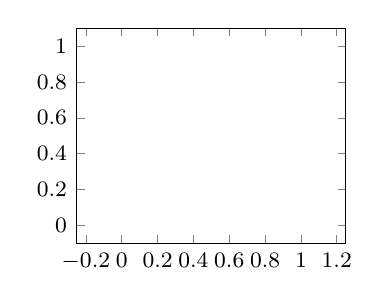
\begin{tikzpicture} 
\begin{axis}[footnotesize,font=\footnotesize,view={\q}{20}
  ,axis equal, axis lines=box ] 
  \node[below] at (axis cs:0,0,0) {$O$};
  \threev{1.54}{0.70}{0.38}{\av}
  \threev{1.19}{-1.25}{0.15}{\bv}
  \threev{1.95}{0.21}{-0.39}{\cv}
\end{axis}
\end{tikzpicture}}
\end{center}
\end{solution}
\end{example}



\begin{proof} 
To prove the angle \autoref{thm:anglev}, form a triangle from vectors \uv, \vv\ and \(\uv-\vv\) as illustrated in the margin.
\marginpar{%
\def\vecopsHook{\node[above] at (axis cs:0,0) {$\qquad\theta$};}
\vecops37{-1}35}%
Recall and apply the \idx{cosine rule} for triangles
\begin{equation*}
|\uv-\vv|^2=|\uv|^2+|\vv|^2-2|\uv||\vv|\cos\theta\,.
\end{equation*}
In \(\RR^n\) this rule rearranges to
\begin{eqnarray*}
2|\uv||\vv|\cos\theta
&=&|\uv|^2+|\vv|^2-|\uv-\vv|^2
\\&=&u_1^2+u_2^2+\cdots+u_n^2
+v_1^2+v_2^2+\cdots+v_n^2
\\&&{}
-(u_1-v_1)^2-(u_2-v_2)^2-\cdots-(u_n-v_n)^2
\\&=&u_1^2+u_2^2+\cdots+u_n^2
+v_1^2+v_2^2+\cdots+v_n^2
\\&&{}
-u_1^2+2u_1v_1-v_1^2-u_2^2+2u_2v_2-v_2^2
\\&&{}
-\cdots-u_n^2+2u_nv_n-v_n^2
\\&=&2u_1v_1+2u_2v_2+\cdots+2u_nv_n
\\&=&2(\lincomb uvn)
\\&=&2\uv\cdot\vv\,.
\end{eqnarray*}
Dividing both sides by \(2|\uv||\vv|\) gives \(\cos\theta=\frac{\uv\cdot\vv}{|\uv||\vv|}\) as required.
\end{proof}





\subsection{Work done involves the dot product}
\label{sec:wdidp}
\index{work done|(}

In physics and engineering, ``work'' has a precise meaning related to energy: when a force of magnitude~\(F\) acts on a body and that body moves a distance~\(d\), then the \idx{work done} by the force is \(W=Fd\)\,.
This formula applies only for one dimensional force and displacement, the case when the force and the displacement are all in the same direction.
For example, if a 5\,kg barbell drops downwards~2\,m under the force of gravity (9.8~newtons/kg), then the work done by gravity on the barbell during the drop is the product
\begin{equation*}
W=F\cdot d=(5\cdot9.8)\cdot 2=98\text{ joules}.
\end{equation*}
This work done goes to the kinetic energy of the falling barbell.
The kinetic energy dissipates when the barbell hits the floor.

\begingroup
\newcommand{\mytemp}[1]{\begin{tikzpicture} 
\begin{axis}[footnotesize,font=\footnotesize
  ,axis equal, axis lines=none
  ] 
  \node[below] at (axis cs:0,0) {$O$};
  \addplot[blue,quiver={u=4,v=1},-stealth,mark=empty] coordinates {(0,0)};
  \node[below] at (axis cs:4,1) {$\dv$};
  \addplot[red,thick,quiver={u=2,v=2},-stealth,mark=empty] coordinates {(0,0)};
  \node[above] at (axis cs:1,1) {$\Fv$};
  \ifnum0<#1
  \addplot[brown,thick] coordinates {(0,0)(40/17,10/17)(2,2)};
  \node[above] at (axis cs:0,0) {$\qquad\theta$};
  \node[below] at (axis cs:1.6,0.4) {$F_0$};
  \fi
\end{axis}
\end{tikzpicture}}
In general, the applied force and the displacement are not in the same direction (as illustrated in the margin).
Consider the general case when a vector force~\Fv\ acts on a body which moves a \idx{displacement vector}~\dv.
\marginpar{\mytemp0}%
Then the work done by the force on the body is the length of the displacement times the component of the force in the direction of the displacement---the component of the force at \idx{right-angles} to the displacement does no work.

As illustrated in the margin, draw a right-angled triangle to decompose the force~\Fv\ into the component~\(F_0\) in the direction of the displacement, and an unnamed component at right-angles.
\marginpar{\mytemp1}%
Then by the scalar formula, the work done is \(W=F_0|\dv|\).
As drawn, the force~\Fv\ makes an angle~\(\theta\) to the displacement~\dv: the dot product determines this angle via \(\cos\theta=(\Fv\cdot\dv)/(|\Fv||\dv|)\)  (\autoref{thm:anglev}).
By basic trigonometry, the adjacent side of the force triangle has length \(F_0=|\Fv|\cos\theta=|\Fv|\frac{\Fv\cdot\dv}{|\Fv||\dv|}=\frac{\Fv\cdot\dv}{|\dv|}\).
Finally, the work done \(W=F_0|\dv|=\frac{\Fv\cdot\dv}{|\dv|}|\dv|=\Fv\cdot\dv\), the dot product of the vector force and vector displacement.
\endgroup

\begin{reduce}
\begin{example} 
A sailing boat travels a distance of~\(40\)\,m East and~\(10\)\,m North, as drawn in the margin.
\marginpar{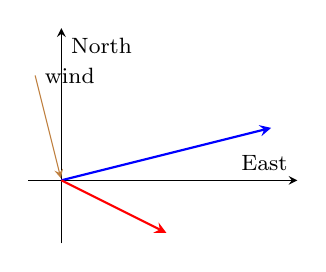
\begin{tikzpicture} 
\begin{axis}[footnotesize,font=\footnotesize
  ,axis equal
  , axis lines=middle, xlabel={East}, ylabel={North}
  ,xtick={0},ytick={0},ymax=29,xmax=45,ymin=-12
  ] 
  \addplot[blue,thick,quiver={u=40,v=10},-stealth,mark=empty] coordinates {(0,0)};
  \node[above] at (axis cs:40,10) {$\dv$};
  \addplot[red,thick,quiver={u=20,v=-10},-stealth,mark=empty] coordinates {(0,0)};
  \node[right] at (axis cs:20,-10) {$\Fv$};
  \addplot[brown,quiver={u=4.9,v=-19.6},-stealth,mark=empty] coordinates {(-5,20)};
  \node[right] at (axis cs:-5,20) {wind};
\end{axis}
\end{tikzpicture}}%
The wind from abeam of strength and direction \((1,-4)\)\,m/s generates a force \(\Fv=(20,-10)\) (newtons) on the sail, as drawn.
What is the work done by the wind?
\begin{solution} 
The direction of the wind is immaterial except for the force it generates.
The displacement vector \(\dv=(40,10)\)\,m.
Then the work done is \(W=\Fv\cdot\dv =(40,10)\cdot(20,-10) =800-100 =700\)~joules.
\end{solution}
\end{example}
\end{reduce}



\begin{activity}
Recall the force of gravity on an object is the mass of the object times the acceleration of gravity,~\(9.8\)\,m/s\({}^2\).
A 3\,kg~ball is thrown horizontally from a height of~2\,m and lands~10\,m away on the ground: what is the total work done by gravity on the ball?
\actposs{\(58.8\) joules}{\(19.6\) joules}{\(29.4\) joules}{\(98\) joules}
\end{activity}


Finding components of vectors in various directions is called projection. 
Such projection is surprisingly common in applications and is developed much further by \autoref{sec:proj}.

\index{work done|)}





\subsection{Algebraic properties of the dot product}
\label{sec:apdp}


To manipulate the dot product in algebraic expressions, we need to know its basic algebraic rules.
The following rules of \autoref{thm:dotops} are analogous to well known rules for scalar multiplication.


\begin{example} 
Given vectors \(\uv=(-2,5,-2)\), \(\vv=(3,3,-2)\) and \(\wv=(2,0,-5)\), and  scalar \(a=2\), verify that (properties~\ref{thm:dotopse} and~\ref{thm:dotopsf})
\begin{itemize}
\item \(a(\uv\cdot\vv)=(a\uv)\cdot\vv=\uv\cdot(a\vv)\) (a form of associativity);
\item \((\uv+\vv)\cdot\wv=\uv\cdot\wv+\vv\cdot\wv\) (\idx{distributivity}).
\end{itemize}
\begin{solution} 
\begin{itemize}
\item For the first:
\begin{eqnarray*}
a(\uv\cdot\vv)&=&2\big((-2,5,-2)\cdot(3,3,-2)\big)
\\&=&2\big((-2)3+5\cdot3+(-2)(-2)\big)
\\&=&2\cdot13=26\,;
\\(a\uv)\cdot\vv&=&(-4,10,-4)\cdot(3,3,-2)
\\&=&(-4)3+10\cdot3+(-4)(-2)
\\&=&26\,;
\\\uv\cdot(a\vv)&=&(-2,5,-2)\cdot(6,6,-4)
\\&=&(-2)6+5\cdot6+(-2)(-4)
\\&=&26\,.
\end{eqnarray*}
These three are equal.

\item For the second:
\begin{eqnarray*}
(\uv+\vv)\cdot\wv&=&(1,8,-4)\cdot(2,0,-5)
\\&=&1\cdot2+8\cdot0+(-4)(-5)
\\&=&22\,;
\\\uv\cdot\wv+\vv\cdot\wv&=&
(-2,5,-2)\cdot(2,0,-5)
\\&&{}
+(3,3,-2)\cdot(2,0,-5)
\\&=&\big[(-2)2+5\cdot0+(-2)(-5)\big]
\\&&{}
+\big[3\cdot2+3\cdot0+(-2)(-5)\big]
\\&=&6+16=22\,.
\end{eqnarray*}
These are both equal.
\end{itemize}
\end{solution}
\end{example}




\begin{theorem}[dot properties] \label{thm:dotops}
For all vectors~\uv, \vv\ and~\wv\ in~\(\RR^n\), and for all scalars~\(a\), the following properties hold:
\begin{enumerate}[ref=\ref{thm:dotops}(\alph*)]
\item\label[theorem]{thm:dotopsa} \(\uv\cdot\vv=\vv\cdot\uv\) \quad(\idx{commutative law});
\item\label[theorem]{thm:dotopsc} \(\uv\cdot\ov=\ov\cdot\uv=0\);
\item\label[theorem]{thm:dotopse} \(a(\uv\cdot\vv)=(a\uv)\cdot\vv=\uv\cdot(a\vv)\);
\item\label[theorem]{thm:dotopsf} \((\uv+\vv)\cdot\wv=\uv\cdot\wv+\vv\cdot\wv\)\quad(\idx{distributive law});
\item\label[theorem]{thm:dotopsg} \(\uv\cdot\uv\geq0\)\,, and moreover, \(\uv\cdot\uv=0\) if and only if \(\uv=\ov\)\,.
\end{enumerate}
\end{theorem}


\begin{proof} 
Here prove only the commutative law~\ref{thm:dotopsa} and the inequality~\ref{thm:dotopsg}.
\autoref{ex:dotops} asks you to analogously prove the other properties.
At the core of each proof is the definition of the dot product which empowers us to deduce a property via the corresponding property for scalars.
\begin{itemize}
\item To prove the commutative law~\ref{thm:dotopsa} consider
\begin{eqnarray*}
\uv\cdot\vv&=&\lincomb uvn \quad(\text{by \autoref{def:dotprod}})
\\&=&\lincomb vun
\\&&\quad(\text{as each scalar multiplication commutes})
\\&=&\vv\cdot\uv \quad(\text{by \autoref{def:dotprod}}).
\end{eqnarray*}

\item To prove the inequality~\ref{thm:dotopsg} consider
\begin{eqnarray*}
\uv\cdot\uv&=&\lincomb uun\quad(\text{by \autoref{def:dotprod}})
\\&=&u_1^2+u_2^2+\cdots+u_n^2
\\&\geq&0+0+\cdots+0 \quad(\text{as each scalar term is}\geq0)
\\&&{}=0\,.
\end{eqnarray*}
To prove the ``moreover'' part, first consider the zero vector.
From \autoref{def:dotprod}, in~\(\RR^n\),
\begin{equation*}
\ov\cdot\ov={0^2+0^2+\cdots+0^2}=0\,.
\end{equation*}
Second, let vector \(\uv=(\hlist un)\) in~\(\RR^n\) satisfy \(\uv\cdot\uv=0\)\,.
Expanding the left-hand side gives that
\begin{equation*}
\underbrace{u_1^2}_{\geq0}+\underbrace{u_2^2}_{\geq0}
+\cdots+\underbrace{u_n^2}_{\geq0}=0\,.
\end{equation*}
Being squares, all terms on the left are non-negative, so the only way they can all add to zero is if they are all zero.
That is, \(u_1=u_2=\cdots=u_n=0\)\,.
Hence, the vector~\uv\ must be the zero vector~\ov.
\end{itemize}
\end{proof}



\begin{activity}
For vectors \(\uv,\vv,\wv\) in~\(\RR^n\), which of the following statements is not generally true?
\actposs[1]{\((2\uv)\cdot(2\vv)=2(\uv\cdot\vv)\)}
{\(\uv\cdot(\vv+\wv)=\uv\cdot\vv+\uv\cdot\wv\)}
{\(\uv\cdot\vv-\vv\cdot\uv=0\)}
{\((\uv-\vv)\cdot(\uv+\vv)=\uv\cdot\uv-\vv\cdot\vv\)}
\end{activity}



The above proof of \autoref{thm:dotopsg}, that \(\uv\cdot\uv=0\) if and only if \(\uv=\ov\)\,, may look uncannily familiar.
The reason is that this last part is essentially the same as the proof of \autoref{thm:veclen0} that the zero vector is the only vector of length zero.
The upcoming \autoref{thm:triscal} establishes that this connection between dot products and lengths is no coincidence.




\begin{example} \label{eg:triscal}
For the two vectors \(\uv=(3,4)\) and \(\vv=(2,1)\) verify the following three properties: 
\begin{enumerate}
\item \(\sqrt{\uv\cdot\uv}=|\uv|\), the \idx{length} of~\uv;
\item \(|\uv\cdot\vv|\leq|\uv||\vv|\) (\idx{Cauchy--Schwarz inequality});
\item \(|\uv+\vv|\leq|\uv|+|\vv|\) (\idx{triangle inequality}).
\end{enumerate}

\begin{solution} 
\begin{enumerate}
\item Here \(\sqrt{\uv\cdot\uv}=\sqrt{3\cdot3+4\cdot4}=\sqrt{25}=5\)\,, whereas the length \(|\uv|=\sqrt{3^2+4^2}=\sqrt{25}=5\) (\autoref{def:veclen}). These expressions are equal.

\item Here \(|\uv\cdot\vv|=|3\cdot2+4\cdot1|=10\)\,, whereas  \(|\uv||\vv|=5\sqrt{2^2+1^2}=5\sqrt5=11.180\)\,.  
Hence \(|\uv\cdot\vv|=10\leq11.180=|\uv||\vv|\).

\item Here \(|\uv+\vv|=|(5,5)|=\sqrt{5^2+5^2}=\sqrt{50}=7.071\)\,, whereas \(|\uv|+|\vv|=5+\sqrt5=7.236\)\,.
Hence \(|\uv+\vv|=7.071\leq7.236=|\uv|+|\vv|\)\,.
\marginpar{\vecops13421}%
This is called the triangle inequality because the vectors~\uv, \vv\ and~\(\uv+\vv\) may be viewed as forming a triangle, as illustrated in the margin, and this inequality follows because the length of a side  of a triangle must be less than the sum of the lengths of the other two sides.
\end{enumerate}
\end{solution}
\end{example}


The \idx{Cauchy--Schwarz inequality} is one point of distinction between this `vector multiplication' and \idx{scalar multiplication}: for scalars \(|ab|=|a||b|\), but the dot product of vectors is typically less, \(|\uv\cdot\vv|\leq|\uv||\vv|\).

\begin{example} 
The general proof of the \idx{Cauchy--Schwarz inequality} involves a trick, so let's introduce the trick using the vectors of \autoref{eg:triscal}.
Let vectors \(\uv=(3,4)\) and \(\vv=(2,1)\) and consider the line given parametrically \index{parametric equation}(\autoref{def:parlin}) as the \idx{position vector}s \(\xv=\uv+t\vv=(3+2t,4+t)\) for scalar parameter~\(t\)---illustrated in the margin.
\marginpar{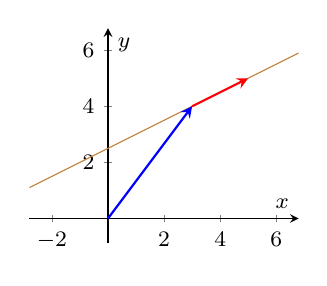
\begin{tikzpicture} 
\begin{axis}[footnotesize,font=\footnotesize
  ,axis equal, axis lines=middle, domain=-2.9:1.9
  ,xlabel={$x$},ylabel={$y$}
  ] 
%\node[left] at (axis cs:0,0) {$O$};
\addplot[brown,no marks] ({3+2*x},{4+x});
\addplot[blue,thick,quiver={u=3,v=4},-stealth] coordinates {(0,0)};
\node[right] at (axis cs:2,3) {$\uv$};
\addplot[red,thick,quiver={u=2,v=1},-stealth] coordinates {(3,4)};
\node[below] at (axis cs:5,5) {$\vv$};
\end{axis}
\end{tikzpicture}}%
The \idx{position vector}~\xv\ of any point on the line has length~\(\ell\) (\autoref{def:veclen}) where
\begin{eqnarray*}
\ell^2&=&(3+2t)^2+(4+t)^2
\\&=&9+12t+4t^2+16+8t+t^2
\\&=&\underbrace{25}_{c}+\underbrace{20}_{b}t+\underbrace{5}_{a}t^2,
\end{eqnarray*}
a quadratic polynomial in~\(t\).
We know that the length~\(\ell>0\)  (the line does not pass through the origin so no~\xv\ is zero).
Hence the quadratic in~\(t\) cannot have any zeros.
By the known properties of \idx{quadratic equation}s it follows that the \idx{discriminant} \(b^2-4ac<0\)\,.
Indeed it is: here \(b^2-4ac=20^2-4\cdot5\cdot25=400-500=-100<0\)\,.
Usefully, here \(a=5=|\vv|^2\), \(c=25=|\uv|^2\) and \(b=20=2\cdot10=2(\uv\cdot\vv)\).
So \(b^2-4ac<0\), rewritten as \(\tfrac14b^2<ac\)\,, becomes the statement that \(\tfrac14[2(\uv\cdot\vv)]^2=(\uv\cdot\vv)^2<|\vv|^2|\uv|^2\).
Taking the square-root of both sides verifies the Cauchy--Schwarz inequality.  
The proof of the next theorem establishes it in general.
\end{example}






\begin{theorem} \label{thm:triscal}
For all vectors \uv\ and \vv\ in~\(\RR^n\) the following properties hold:
\begin{enumerate}[ref=\ref{thm:triscal}(\alph*)]
  \item\label[theorem]{thm:triscala} \(\sqrt{\uv\cdot\uv}=|\uv|\), the \idx{length} of~\uv;
\item\label[theorem]{thm:triscalb} \(|\uv\cdot\vv|\leq|\uv||\vv|\) (\bfidx{Cauchy--Schwarz inequality});
\item\label[theorem]{thm:triscalc} \(|\uv\pm\vv|\leq|\uv|+|\vv|\) (\bfidx{triangle inequality}).
\end{enumerate}
\end{theorem}

\begin{proof} 
Except for the first, each property depends upon the previous.
\begin{description}
\item[\ref{thm:triscala}]
\begin{eqnarray*}
\sqrt{\uv\cdot\uv}&=&\sqrt{\lincomb uun}\quad(\text{by \autoref{def:dotprod}})
\\&=&\sqrt{u_1^2+u_2^2+\cdots+u_n^2}
\\&=&|\uv|\quad(\text{by \autoref{def:veclen}}).
\end{eqnarray*}

\item[\ref{thm:triscalb}]  
To prove the Cauchy--Schwarz inequality between vectors~\uv\ and~\vv\ first consider the trivial case when \(\vv=\ov\): then the left-hand side \(|\uv\cdot\vv|=|\uv\cdot\ov|=|\ov|=0\); whereas the right-hand side \(|\uv||\vv|=|\uv||\ov|=|\uv|0=0\); and so the inequality \(|\uv\cdot\vv|\leq|\uv||\vv|\) is satisfied in this case.

Second, for the case when \(\vv\neq\ov\), consider the line given parametrically by \(\xv=\uv+t\vv\) for (real) scalar parameter~\(t\) (\autoref{def:parlin}), as illustrated in the margin.
\marginpar{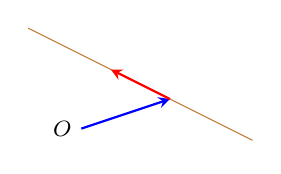
\begin{tikzpicture} 
\begin{axis}[footnotesize,font=\footnotesize
  ,axis equal, axis lines=none, domain=-1.4:2.4 ] 
\node[left] at (axis cs:0,0) {$O$};
\addplot[brown,no marks] ({3-2*x},{1+x});
\addplot[blue,thick,quiver={u=3,v=1},-stealth] coordinates {(0,0)};
\node[below] at (axis cs:2,0.67) {$\uv$};
\addplot[red,thick,quiver={u=-2,v=1},-stealth] coordinates {(3,1)};
\node[above] at (axis cs:2,1.5) {$\vv$};
\end{axis}
\end{tikzpicture}}%
The distance~\(\ell\) of a point on the line from the origin is the length of its position vector, and by property~\ref{thm:triscala}
\begin{eqnarray*}
\ell^2&=&\xv\cdot\xv
\\&=&(\uv+t\vv)\cdot(\uv+t\vv)
\\&&\quad(\text{then using distributivity~\ref{thm:dotopsf}})
\\&=&\uv\cdot(\uv+t\vv)+(t\vv)\cdot(\uv+t\vv)
\\&&\quad(\text{again using distributivity~\ref{thm:dotopsf}})
\\&=&\uv\cdot\uv+\uv\cdot(t\vv)+(t\vv)\cdot\uv+(t\vv)\cdot(t\vv)
\\&&\quad(\text{using scalar mult.\ property~\ref{thm:dotopse}})
\\&=&\uv\cdot\uv+t(\uv\cdot\vv)+t(\vv\cdot\uv)+t^2(\vv\cdot\vv)
\\&&\quad(\text{using~\ref{thm:triscala} and commutativity~\ref{thm:dotopsa}})
\\&=&|\uv|^2+2(\uv\cdot\vv)t+|\vv|^2t^2
\\&=&at^2+bt+c,
\end{eqnarray*}
a quadratic in~\(t\), with coefficients \(a=|\vv|^2>0\), \(b=2(\uv\cdot\vv)\), and \(c=|\uv|^2\).
Since \(\ell^2\geq0\) (it may be zero if the line goes through the origin), then this quadratic in~\(t\) has either no zeros or just one zero.
By the properties of quadratic equations, the \idx{discriminant} \(b^2-4ac\leq0\)\,, that is, \(\tfrac14b^2\leq ac\)\,.
Substituting the particular coefficients here gives 
\(\tfrac14\big[2(\uv\cdot\vv)\big]^2=(\uv\cdot\vv)^2\leq|\vv|^2|\uv|^2\).
Taking the square-root of both sides then establishes the Cauchy--Schwarz inequality  \(|\uv\cdot\vv|\leq|\uv||\vv|\).

\item[\ref{thm:triscalc}]
To prove the triangle inequality between vectors~\uv\ and~\vv\ first observe the Cauchy--Schwarz inequality implies \((\uv\cdot\vv)\leq|\uv||\vv|\) (since the left-hand side has magnitude\({}\leq{}\)the right-hand side).
Then consider (analogous to the \(t=1\) case of the above)
\marginpar{\vecops131{-2}2}%
\begin{eqnarray*}
|\uv+\vv|^2
&=&(\uv+\vv)\cdot(\uv+\vv)
\\&&\quad(\text{then using distributivity~\ref{thm:dotopsf}})
\\&=&\uv\cdot(\uv+\vv)+\vv\cdot(\uv+\vv)
\\&&\quad(\text{again using distributivity~\ref{thm:dotopsf}})
\\&=&\uv\cdot\uv+\uv\cdot\vv+\vv\cdot\uv+\vv\cdot\vv
\\&&\quad(\text{using~\ref{thm:triscala} and commutativity~\ref{thm:dotopsa}})
\\&=&|\uv|^2+2(\uv\cdot\vv)+|\vv|^2
\\&&\quad(\text{using Cauchy--Schwarz inequality})
\\&\leq&|\uv|^2+2|\uv||\vv|+|\vv|^2
\\&&{}=(|\uv|+|\vv|)^2.
\end{eqnarray*}
Take the square-root of both sides to establish the triangle inequality \(|\uv+\vv|\leq|\uv|+|\vv|\).

The minus case follows because \(|\uv-\vv|=|\uv+(-\vv)|\leq|\uv|+|-\vv|=|\uv|+|\vv|\).
\marginpar{\vecops331{-2}2}%

\end{description}
\end{proof}


\begin{example} 
Verify the \idx{Cauchy--Schwarz inequality} and the \idx{triangle inequality} (\(+\)~case) for the vectors \(\av=(-1,-2,1,3,-2)\) and \(\bv=(-3,-2,10,2,2)\).
\begin{solution} 
We need the length of the vectors:
\begin{eqnarray*}
|\av|&=&\sqrt{(-1)^2+(-2)^2+1^2+3^2+(-2)^2}
\\&=&\sqrt{19}=4.3589,
\\|\bv|&=&\sqrt{(-3)^2+(-2)^2+10^2+2^2+2^2}
\\&=&\sqrt{121}=11\,,
\end{eqnarray*}
and also the dot product
\begin{eqnarray*}
\av\cdot\bv
&=&(-1)(-3)+(-2)(-2)+1\cdot10+3\cdot2+(-2)2
\\&=&19\,.
\end{eqnarray*}
Hence \(|\av\cdot\bv|=19<47.948=|\av||\bv|\), which verifies the Cauchy--Schwarz inequality.

Now, the length of the sum
\begin{eqnarray*}
|\av+\bv|&=&|(-4,-4,11,5,0)|
\\&=&\sqrt{(-4)^2+(-4)^2+11^2+5^2+0^2}
\\&=&\sqrt{178}=13.342\,.
\end{eqnarray*}
Here \(|\av+\bv|=13.342\) whereas \(|\av|+|\bv|=11+\sqrt{19}=15.359\)\,.
Hence verifies the triangle inequality \(|\av+\bv|\leq|\av|+|\bv|\).
\end{solution}
\end{example}








\subsection{Orthogonal vectors are at right-angles}
\label{sec:ovra}

\index{orthogonal vectors|(}
\index{right-angles|(}

Of all the angles that vectors can make with each other, the two most important angles are, firstly, when the vectors are aligned with each other, and secondly, when the vectors are at right-angles to each other.
Recall \autoref{thm:anglev} gives the angle~\(\theta\) between two vectors via \(\cos\theta=\frac{\uv\cdot\vv}{|\uv||\vv|}\).
For vectors at \idx{right-angles} \(\theta=90^\circ\),  so \(\cos\theta=0\)\,, and hence nonzero vectors are at right-angles only when the dot product \(\uv\cdot\vv=0\)\,.
We give a special name to vectors at right-angles.


\begin{definition} \label{def:orthovec}
Two vectors~\uv\ and~\vv\ in~\(\RR^n\) are termed
\bfidx{orthogonal} (or \bfidx{perpendicular})
if and only if their dot product \(\uv\cdot\vv=0\)\,.
\begin{aside}
The term `orthogonal' derives from the Greek for `right-angled'.
\end{aside}%
\end{definition}

By convention the \idx{zero vector}~\ov\ is orthogonal to all other vectors.
However, in practice, we almost always use the notion of orthogonality only in connection with \emph{nonzero} vectors.
Often the requirement that the orthogonal vectors are nonzero is explicitly made, but beware that sometimes the requirement may be implicit in the problem.


\begin{example} 
The \idx{standard unit vector}s (\autoref{def:stuniv}) are orthogonal to each other.
For example, consider the standard unit vectors~\iv, \jv\ and~\kv\ in~\(\RR^3\):
\index{i@$\iv$}\index{j@$\jv$}\index{k@$\kv$}%
\begin{itemize}
\item \(\iv\cdot\jv=(1,0,0)\cdot(0,1,0)=0+0+0=0\);
\item \(\jv\cdot\kv=(0,1,0)\cdot(0,0,1)=0+0+0=0\);
\item \(\kv\cdot\iv=(0,0,1)\cdot(1,0,0)=0+0+0=0\).
\end{itemize}
By \autoref{def:orthovec} these are orthogonal to each other.
\end{example}


\begin{example} 
Which pairs of the following vectors, if any, are \idx{perpendicular} to each other?
\(\uv=(-1,1,-3,0)\), \(\vv=(2,4,2,-6)\) and \(\wv=(-1,6,-2,3)\).
\begin{solution} 
Is the dot product zero? or not?
\begin{itemize}
\item \(\uv\cdot\vv =(-1,1,-3,0)\cdot(2,4,2,-6) =-2+4-6+0 =-4 \neq0\) so this pair are not perpendicular. 
\item \(\uv\cdot\wv =(-1,1,-3,0)\cdot(-1,6,-2,3) =1+6+6+0 =13 \neq0\) so this pair are not perpendicular. 
\item \(\vv\cdot\wv =(2,4,2,-6)\cdot(-1,6,-2,3) =-2+24-4-18 =0\) so this pair of vectors are perpendicular to each other. 
\end{itemize}
\end{solution}
\end{example}



\begin{activity}
Which pair of the following three vectors are orthogonal to each other?
\(\xv=\iv-2\kv\)\,, \(\yv=-3\iv-4\jv\)\,, \(\zv=-\iv-2\jv+2\kv\)
\actposs[4]{no pair}{\(\yv,\zv\)}{\(\xv,\zv\)}{\(\xv,\yv\)}
\end{activity}



\begin{reduce}
\begin{example} 
Find the scalar number~\(b\) such that vectors \(\av=\iv+4\jv+2\kv\) and \(\bv=\iv+b\jv-3\kv\) are at \idx{right-angles}.
\begin{solution} 
For vectors to be at right-angles, their dot product must be zero.
Hence find~\(b\) such that
\begin{equation*}
0=\av\cdot\bv=(\iv+4\jv+2\kv)\cdot(\iv+b\jv-3\kv)
=1+4b-6=4b-5\,.
\end{equation*}
Solving \(0=4b-5\) gives \(b=5/4\).
That is, \(\iv+\tfrac54\jv-3\kv\) is at right-angles to \(\iv+4\jv+2\kv\).
\end{solution}
\end{example}
\end{reduce}



\paragraph{Key properties}
The next couple of innocuous looking theorems are vital keys to important results in subsequent chapters.

\index{i@$\iv$}\index{j@$\jv$}%
To introduce the first theorem, consider the 2D plane and try to draw a nonzero vector at \idx{right-angles} to both the two \idx{standard unit vector}s~\iv\ and~\jv.
\marginpar{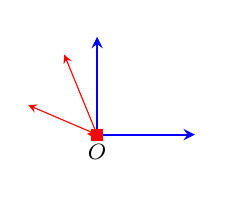
\begin{tikzpicture} 
\begin{axis}[footnotesize,font=\footnotesize
  ,axis equal, axis lines=none
  ,ymin=-1.1,xmin=-1.1,xmax=1.1,ymax=1.1
  ] 
  \node[below] at (axis cs:0,0) {$O$};
  \addplot[blue,thick,quiver={u=1,v=0},-stealth] coordinates {(0,0)};
  \node[above] at (axis cs:1,0) {$\iv$};
  \addplot[blue,thick,quiver={u=0,v=1},-stealth,forget plot] coordinates {(0,0)};
  \node[right] at (axis cs:0,1) {$\jv$};
  \addplot+[quiver={u=rand,v=rand},-stealth] coordinates {(0,0)(0,0)(0,0)};
\end{axis}
\end{tikzpicture}}%
The red vectors in the margin illustrate failed attempts to draw a nonzero vector at right-angles to both~\iv\ and~\jv.
It cannot be done. 
No vector in the plane can be at right-angles to both the standard unit vectors in the plane.


\begin{theorem} \label{thm:nononz}
There is no nonzero vector \idx{orthogonal} to all \(n\)~\idx{standard unit vector}s in~\(\RR^n\).
\end{theorem}

\begin{proof} 
Let \(\uv=(\hlist un)\) be a vector in~\(\RR^n\) that is orthogonal to all \(n\)~standard unit vectors.  
Then by \autoref{def:orthovec} of orthogonality:
\begin{itemize}
\item \(0=\uv\cdot\ev_1=(\hlist un)\cdot(1,0,\ldots,0)=u_1+0+\cdots+0=u_1\), and so the first component must be zero;
\item \(0=\uv\cdot\ev_2=(\hlist un)\cdot(0,1,\ldots,0)=0+u_2+0+\cdots+0=u_2\), and so the second component must be zero; 
\item and so on to
\item \(0=\uv\cdot\ev_n=(\hlist un)\cdot(0,0,\ldots,1)=0+0+\cdots+u_n=u_n\), and so the last component must be zero.
\end{itemize}
Since \(u_1=u_2=\cdots=u_n=0\) the only vector that is orthogonal to all the standard unit vectors is \(\uv=\ov\), the zero vector.
\end{proof}


To introduce the second theorem, 
\marginpar{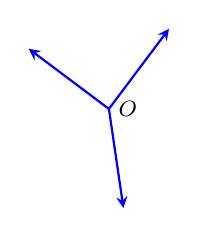
\begin{tikzpicture} 
\begin{axis}[footnotesize,font=\footnotesize
  ,axis equal, axis lines=none
  ] 
  \node[right] at (axis cs:0,0) {$O$};
  \addplot[blue,thick,quiver={u=0.6,v=0.8},-stealth] coordinates {(0,0)};
  \addplot[blue,thick,quiver={u=-0.8,v=0.6},-stealth] coordinates {(0,0)};
  \addplot[blue,thick,quiver={u=0.145,v=-0.989},-stealth] coordinates {(0,0)};
\end{axis}
\end{tikzpicture}}%
imagine trying to draw three unit vectors in any orientation in the 2D plane such that all three are at \idx{right-angles} to each other.
The margin illustrates one attempt.
It cannot be done.
There are at most two vectors in 2D that are all at right-angles to each other.


\begin{theorem}[orthogonal completeness] \label{thm:orthcomp}
In a set of \idx{orthogonal} \idx{unit vector}s in~\(\RR^n\), there can be no more than \(n\)~vectors in the set.
\footnote{For the pure at heart, this property is part of the definition of what we mean by~\(\RR^n\).  
The representation of a vector in~\(\RR^n\) by \(n\)~components (here \autoref{def:vecs}) then follows as a consequence, instead of vice-versa as here.}
\end{theorem}


\begin{proof} 
Use \idx{contradiction}%
\ifcsname r@sec:pc\endcsname\ (\autoref{sec:pc})\fi.
Suppose there are more than \(n\)~orthogonal unit vectors in the set.
\marginpar{\rotatebox{53.10}{\begin{tikzpicture} 
\begin{axis}[footnotesize,font=\footnotesize
  ,axis equal image, axis lines=middle,xtick={-1,0,1},ytick={-1,0,1}
  ,ymin=-1.4,ymax=1.4,xmin=-1.4,xmax=1.4 ] 
  \node[below] at (axis cs:0,0) {$\quad O$};
  \addplot[blue,thick,quiver={u=1,v=0},-stealth] coordinates {(0,0)};
  \node[above] at (axis cs:1,0) {$\ev_1$};
  \addplot[blue,thick,quiver={u=0,v=1},-stealth] coordinates {(0,0)};
  \node[right] at (axis cs:0,1) {$\ev_2$};
  \addplot[blue,thick,quiver={u=-0.704,v=-0.710},-stealth] coordinates {(0,0)};
\end{axis}
\end{tikzpicture}}}%
Define a coordinate system for~\(\RR^n\) using the first~\(n\) of the given unit vectors as the \(n\)~standard unit vectors 
(as illustrated for~\(\RR^2\) in the margin).
\autoref{thm:nononz} then says there cannot be any more nonzero vectors orthogonal than these \(n\)~standard unit vectors.
This contradicts there being more than~\(n\) orthogonal unit vectors.
To avoid this contradiction the supposition must be wrong; that is, there cannot be more than~\(n\) orthogonal unit vectors in~\(\RR^n\).
\end{proof}


\index{orthogonal vectors|)}
\index{right-angles|)}






\subsection{Normal vectors and equations of a plane}
\label{sec:nvep}

\index{normal vector|(}

This section uses the dot product to find equations of a plane in~3D.
The key is to write points in the plane as all those at \idx{right-angles} to a certain direction.  
This direction is \idx{perpendicular} to the required plane, and is called a normal.
Let's start with an example of the idea in 2D.

\begin{example} 
First find the equation of the line that is \idx{perpendicular} to the vector~\((2,3)\) and that passes through the origin.
Second, find the equation of the line that passes through the point~\((4,1)\) (instead of the origin).
\begin{solution} 
Recall that vectors at right-angles have a zero dot product (\autoref{sec:ovra}).
\marginpar{\begin{tikzpicture} 
\begin{axis}[footnotesize,font=\footnotesize
  ,axis equal, axis lines=middle, xlabel={$x$}, ylabel={$y$}
  ] 
  \addplot[brown,thick,mark=empty] {-2/3*x};
  \addplot[blue,thick,quiver={u=2,v=3},-stealth,mark=empty] coordinates {(0,0)};
  \node[right] at (axis cs:2,3) {$(2,3)$};
  \addplot[red,thick,quiver={u=-3,v=2},-stealth,mark=empty] coordinates {(0,-0.1)};
  \node[above] at (axis cs:-3,2) {$\xv$};  
\end{axis}
\end{tikzpicture}}
Thus the position vector~\xv\ of every point in the line satisfies the dot product \(\xv\cdot(2,3)=0\)\,.
For \(\xv=(x,y)\), as illustrated in the margin, \(\xv\cdot(2,3)=2x+3y\) so the equation of the line is \(2x+3y=0\)\,.

When the line goes through \((4,1)\) (instead of the origin), then it is the displacement vector \(\xv-(4,1)\) that must be orthogonal to~\((2,3)\), as illustrated.
\marginpar{\begin{tikzpicture} 
\begin{axis}[footnotesize,font=\footnotesize, domain=-1:9
  ,axis equal, axis lines=middle, xlabel={$x$}, ylabel={$y$}
  ] 
  \addplot[brown,thick,mark=empty] {-2/3*(x-4)+1};
  \addplot[blue,thick,quiver={u=2,v=3},-stealth,mark=empty] coordinates {(4,1)};
  \node[right] at (axis cs:6,4) {$(2,3)$};
  \addplot[red,quiver={u=4,v=1},-stealth,mark=empty] coordinates {(0,0)};
  \node[right] at (axis cs:4,1) {$(4,1)$};
  \addplot[red,quiver={u=1,v=3},-stealth,mark=empty] coordinates {(0,0)};
  \node[right] at (axis cs:0.5,1.5) {$\vec x$};
  \addplot[red,thick,quiver={u=-3,v=2},-stealth,mark=empty] coordinates {(4,0.95)};
  \node[right] at (axis cs:1.3,2.8) {$\vec x-(4,1)$};
\end{axis}
\end{tikzpicture}}
That is, the equation of the line is \((x-4,y-1)\cdot(2,3)=0\).
Evaluating the dot product gives \(2(x-4)+3(y-1)=0\); that is, \(2x+3y=2\cdot4+3\cdot1=11\) is an equation of the line.
\end{solution}
\end{example}





\begin{activity}
What is an equation of the line  that is both through the point~\((4,2)\), and at \idx{right-angles} to the vector~\((1,3)\)?
\actposs{\(x+3y=10\)}{\(4x+2y=10\)}{\(4x+y=11\)}{\(2x+3y=11\)}
\end{activity}





\begingroup\newcommand{\mytmp}[1]{%
\qview{20}{25}{\begin{tikzpicture} 
\begin{axis}[footnotesize,font=\footnotesize, height=5cm, view={\q}{20}
  , domain=-1.5:3.5, axis equal, axis lines=box
  ] 
  \ifnum0<#1
  \addplot3[red,quiver={u=1,v=1,w=2},-stealth,mark=empty] coordinates {(0,0,0)};
  \node[left] at (axis cs:0.7,0.7,1.4) {$\pv$};
  \addplot3[red,quiver={u=3,v=1.5,w=1.5},-stealth,mark=empty] coordinates {(0,0,0)};
  \node[right] at (axis cs:1,0.5,0.5) {$\xv$};
  \node[left] at (axis cs:0,0,0) {$O$};
  \fi
  \addplot3[surf,samples=9,opacity=0.4] {2-(x-1)/3+(y-1)/3};
  \addplot3[blue,thick,quiver={u=1,v=-1,w=3},-stealth,mark=empty] coordinates {(1,1,2)};
  \node[left] at (axis cs:2,0,5) {$\nv$};
  \addplot3[mark=*] coordinates {(1,1,2)} node[left] {$P$};
  \addplot3[red,thick,quiver={u=2,v=0.5,w=-0.5},-stealth,mark=empty] coordinates {(1,1,2)};
  \addplot3[mark=*] coordinates {(3,1.5,1.5)} node[right] {$X$};
  \ifnum0<#1
  \node[above] at (axis cs:2.6,1.3,1.7) {$\xv-\pv$};
  \fi
\end{axis}
\end{tikzpicture}}}
Now use the same approach to finding an equation of a plane in~3D.
The problem is to find the \idx{equation of the plane} that goes through a given point~\(P\) and is \idx{perpendicular} to a given vector~\nv, called a \bfidx{normal vector}.
As illustrated in stereo below, that means to find all points~\(X\) such that~\(\ovect{PX}\) is orthogonal to~\nv.
\begin{center}\mytmp0\end{center}
Denote the position vector of~\(P\) by~\(\pv=(x_0,y_0,z_0)\),  the position vector of~\(X\) by \(\xv=(x,y,z)\), and let the \idx{normal vector} be \(\nv=(a,b,c)\).
Then, as drawn below, the \idx{displacement vector} \(\ovect{PX}=\xv-\pv=(x-x_0,y-y_0,z-z_0)\) and so for \(\ovect{PX}\) to be orthogonal to~\nv\ requires \(\nv\cdot(\xv-\pv)=0\); that is, an \bfidx{equation of the plane} is
\begin{equation*}
a(x-x_0)+b(y-y_0)+c(z-z_0)=0\,,
\end{equation*}
equivalently, an \idx{equation of the plane} is
\begin{equation*}
ax+by+cz=d
\quad\text{for constant }d=ax_0+by_0+cz_0\,.
\end{equation*}
\begin{center}\mytmp1\end{center}
\endgroup



\begin{example} 
Find an \idx{equation of the plane} through point \(P=(1,1,2)\) that has \idx{normal vector} \(\nv=(1,-1,3)\).
(This is the case in the above illustrations.)
Hence write down three distinct points on the plane.
\begin{solution} 
Letting \(\xv=(x,y,z)\) be the coordinates of a point in the plane, the above argument asserts an equation of the plane is \(\nv\cdot(\xv-\ovect{OP})=0\) which becomes
\(1(x-1)-1(y-1)+3(z-2)=0\); that is, \(x-1-y+1+3z-6=0\)\,, which rearranged is \(x-y+3z=6\)\,. 

To find some points in the plane, rearrange this equation to \(z=2-x/3+y/3\) and then substitute any values for~\(x\) and~\(y\):  
\(x=y=0\) gives \(z=2\) so \((0,0,2)\) is on the plane; 
\(x=3\) and \(y=0\) gives \(z=1\) so \((3,0,1)\) is on the plane;
\(x=2\) and \(y=-2\) gives \(z=2/3\) so \((2,-2,\frac23)\) is on the plane; and so on.
\end{solution}
\end{example}





\begin{reduce}
\begin{example} 
Write down a \idx{normal vector} to each of the following planes:
\begin{Parts}
\item \(3x-6y+2z=4\)\,;
\item \(z=0.2x-3.3y-1.9\)\,.
\end{Parts}
\begin{solution} \ 
\begin{enumerate}
\item In this standard form \(3x-6y+2z=4\) a normal vector is the coefficients of the variables, \(\nv=(3,-6,2)\) (or any scalar multiple).
\item Rearrange \(z=0.2x-3.3y-1.9\) to standard form \(-0.2x+3.3y+z=-1.9\) then a normal is \(\nv=(-0.2,3.3,1)\) (or any scalar multiple).
\end{enumerate} 
\end{solution}
\end{example}
\end{reduce}




\begin{activity}
Which of the following is a normal vector to the plane \(x_2+2x_3+4=x_1\)\,?
\actposs{\((-1,1,2)\)}{\((1,2,1)\)}{\((1,2,4)\)}{none of these}
\end{activity}




\index{normal vector|)}




\index{parametric equation|(}
\paragraph{Parametric equation of a plane}
An alternative way of describing a plane is via a parametric equation analogous to the parametric equation of a line (\autoref{sec:pel}).
Such a parametric representation generalizes to every dimension (\autoref{sec:lcss}).

The basic idea, as illustrated in the margin, is that given any plane (through the origin for the moment), then choosing almost any two vectors in the plane allows us to write all points in the plane as a \idx{sum} of multiples of the two vectors.
With the given vectors~\uv\ and~\vv\ shown in the margin, illustrated are the points \(\uv+2\vv\), \(\tfrac12\uv-2\vv\) and \(-2\uv+3\vv\).
\marginpar{\begin{tikzpicture}
\newcommand{\ppoint}[2]{
    \pgfmathparse{#1*3+#2*1}\let\h\pgfmathresult
    \pgfmathparse{#1*1+#2*2}\let\v\pgfmathresult
    \addplot[red,mark=*,only marks] coordinates {(\h,\v)};
    \edef\temp{\noexpand
    \node[below] at (axis cs:\h,\v) {$#1\noexpand\uv{#2}\noexpand\vv$};
    }\temp
    }
\begin{axis}[footnotesize,font=\footnotesize
  ,axis lines=none%,xlabel={$x$},ylabel={$y$}
  , axis equal
  , view={0}{90}
  ,xmax=7.5,ymax=5.5,xmin=-7.5,ymin=-5.5
  ]
\addplot3[mesh,brown,samples=17,domain=-4:4,dotted] (3*x+y,x+2*y,0);
\addplot3[mesh,brown,samples=9,domain=-4:4] (3*x+y,x+2*y,0);
\addplot[blue,quiver={u=3,v=1},-stealth,thick] coordinates {(0,0)};
\node[right] at (axis cs:3,1) {$\uv$};
\addplot[blue,quiver={u=1,v=2},-stealth,thick] coordinates {(0,0)};
\node[above] at (axis cs:1,2) {$\vv$};
\node[left] at (axis cs:0,0) {$O$};
\ppoint{1}{+2}
\ppoint{0.5}{-2}
\ppoint{-2}{+3}
\end{axis}
\end{tikzpicture}}%
Similarly, all points in the plane have a \idx{position vector} in the form \(s\uv+t\vv\) for some scalar parameters~\(s\) and~\(t\).
The grid shown in the margin illustrates the sum of integral and half-integral multiples.
The formula \(\xv=s\uv+t\vv\) for parameters~\(s\) and~\(t\) is called a parametric \idx{equation of the plane}.




\begin{example} 
Find a parametric \idx{equation of the plane} that passes through the three points \(P=(-1,2,3)\), \(Q=(2,3,2)\) and \(R=(0,4,5)\), drawn below in stereo.
\newcommand{\mytemp}[1]{%
\qview{50}{55} {\begin{tikzpicture}
\begin{axis}[footnotesize,font=\footnotesize,height=5cm
  ,axis lines=box, axis equal, view={\q}{25} ]
\addplot3[black,mark=*,only marks,nodes near coords
,nodes near coords align={above}
,point meta=explicit symbolic] coordinates {
(-1,2,3)[$P$] (2,3,2)[$Q$] (0,4,5)[$R$] };
\addplot3[surf,opacity=0.5,samples=9,domain=-0.9:1.9] (3*x+y-1,x+2*y+2,-x+2*y+3);
\ifnum0<#1
\addplot3[blue,quiver={u=-1,v=2,w=3},-stealth,thick] coordinates {(0,0,0)};
\node[left] at (axis cs:-0.5,1,1.5) {$\pv$};
\node[left] at (axis cs:0,0,0) {$O$};
\addplot3[blue,quiver={u=3,v=1,w=-1},-stealth,thick] coordinates {(-1,2,3)};
\node[below] at (axis cs:0.5,2.5,2.5) {$\uv$};
\addplot3[blue,quiver={u=1,v=2,w=2},-stealth,thick] coordinates {(-1,2,3)};
\node[below] at (axis cs:-0.33,3.33,4.33) {$\vv$};
\fi
\end{axis}
\end{tikzpicture}}}
\begin{center}\mytemp0\end{center}

\begin{solution} 
This plane does not pass through the origin, so we first choose a point and make the description relative to that point: say we choose the point~\(P\) with position vector \(\pv=\ovect{OP}=-\iv+2\jv+3\kv\).
Then, as illustrated below, two vectors parallel to the required plane are 
\begin{eqnarray*}
\uv&=&\ovect{PQ} =\ovect{OQ}-\ovect{OP} 
\\&=&(2\iv+3\jv+2\kv)-(-\iv+2\jv+3\kv) 
\\&=&3\iv+\jv-\kv,
\\\vv&=&\ovect{PR} =\ovect{OR}-\ovect{OP} 
\\&=&(4\jv+5\kv)-(-\iv+2\jv+3\kv) 
\\&=&\iv+2\jv+2\kv.
\end{eqnarray*}
\begin{center}\mytemp1\end{center} 
Lastly, every point in the plane is the sum of the displacement vector~\pv\ and arbitrary multiples of the parallel vectors~\uv\ and~\vv.
That is, a parametric equation of the plane is \(\xv=\pv+s\uv+t\vv\) which here is
\begin{eqnarray*}
\xv&=&(-\iv+2\jv+3\kv)+s(3\iv+\jv-\kv)+t(\iv+2\jv+2\kv)
\\&=&(-1+3s+t)\iv+(2+s+2t)\jv+(3-s+2t)\kv.
\end{eqnarray*}
\end{solution}
\end{example}




\begin{definition} \label{def:parpla}
A \bfidx{parametric equation} of a plane is \(\xv=\pv+s\uv+t\vv\) where \pv~is the \idx{position vector} of some point in the plane,   the two vectors~\uv\ and~\vv\ are parallel to the plane (\(\uv,\vv\neq\ov\) and are at a nonzero\slash non-\(\pi\) \idx{angle} to each other), and the scalar \bfidx{parameter}s~\(s\) and~\(t\) vary over all real values to give \idx{position vector}s of all points in the plane.
\end{definition}

The beauty of this definition is that it applies for planes in any number of dimensions.
To do so the \idx{parametric equation}s just uses two vectors with the corresponding number of components.



\begin{example} 
Find a parametric \idx{equation of the plane} that passes through the three points \(P=(6,-4,3)\), \(Q=(-4,-18,7)\) and \(R=(11,3,1)\), drawn below in stereo.
\begin{center}
\qview{50}{55} {\begin{tikzpicture}
\begin{axis}[footnotesize,font=\footnotesize,height=5cm
  ,axis lines=box, axis equal, view={\q}{25} ]
\addplot3[black,mark=*,only marks,nodes near coords
,nodes near coords align={above}
,point meta=explicit symbolic] coordinates {
(6,-4,3)[$P$] (-4,-18,7)[$Q$] (11,3,1)[$R$] };
\end{axis}
\end{tikzpicture}}
\end{center}

\begin{solution} 
First choose a point and make the description relative to that point: say choose point~\(P\) with position vector \(\pv=\ovect{OP}=6\iv-4\jv+3\kv\).
Then, as illustrated below, two vectors parallel to the required plane are 
\begin{eqnarray*}
\uv&=&\ovect{PQ} =\ovect{OQ}-\ovect{OP} 
\\&=&(-4\iv-18\jv+7\kv)-(6\iv-4\jv+3\kv) 
\\&=&-10\iv-14\jv+4\kv,
\\\vv&=&\ovect{PR} =\ovect{OR}-\ovect{OP} 
\\&=&(11\iv+3\jv+\kv)-(6\iv-4\jv+3\kv) 
\\&=&5\iv+7\jv-2\kv.
\end{eqnarray*}
Oops: notice that \(\uv=-2\vv\) so the vectors~\uv\ and~\vv\ are not at a nontrivial angle; instead they are aligned along a line because the three points~\(P\), \(Q\) and~\(R\) are collinear.
There are an infinite number of planes passing through such collinear  points.
Hence we cannot answer the question which requires ``the plane''.
\end{solution}
\end{example}



\begin{example} 
Find a parametric \idx{equation of the plane} that passes through the three points \(A=(-1.2,2.4,0.8)\), \(B=(1.6,1.4,2.4)\) and \(C=(0.2,-0.4,-2.5)\), drawn below in stereo.
%Hence determine if the point \(D=(6.7,1.5,2.3)\) is in the plane, or not.
\newcommand{\mytemp}[1]{%
\qview{10}{15} {\begin{tikzpicture}
\begin{axis}[footnotesize,font=\footnotesize,height=5cm
  ,axis lines=box, axis equal, view={\q}{20} ]
\addplot3[black,mark=*,only marks,nodes near coords
,nodes near coords align={above}
,point meta=explicit symbolic] coordinates {
(-1.2,2.4,0.8)[$A$] (1.6,1.4,2.4)[$B$] (0.2,-0.4,-2.5)[$C$] };
\addplot3[surf,opacity=0.5,samples=9,domain=-0.1:1.1] (-1.2+2.8*x+1.4*y,2.4-x-2.8*y,0.8+1.6*x-3.3*y);
\ifnum0<#1
\addplot3[blue,quiver={u=-1.2,v=2.4,w=0.8},-stealth,thick] coordinates {(0,0,0)};
\node[right] at (axis cs:-0.6,1.2,0.4) {$a$};
\node[right] at (axis cs:0,0,0) {$O$};
\addplot3[blue,quiver={u=2.8,v=-1,w=1.6},-stealth,thick] coordinates {(-1.2,2.4,0.8)};
\node[below] at (axis cs:0.2,1.9,1.6) {$u$};
\addplot3[blue,quiver={u=1.4,v=-2.8,w=-3.3},-stealth,thick] coordinates {(-1.2,2.4,0.8)};
\node[left] at (axis cs:-0.5,1,-0.85) {$v$};
\fi
\end{axis}
\end{tikzpicture}}}
\begin{center}\mytemp0\end{center}
\begin{solution} 
First choose a point and make the description relative to that point: say we choose the point~\(A\) with position vector \(\av=\ovect{OA}=-1.2\iv+2.4\jv+0.8\kv\).
Then, as illustrated below, two vectors parallel to the required plane are 
\begin{eqnarray*}
\uv&=&\ovect{AB} =\ovect{OB}-\ovect{OA} 
\\&=&(1.6\iv+1.4\jv+2.4\kv)-(-1.2\iv+2.4\jv+0.8\kv) 
\\&=&2.8\iv-\jv+1.6\kv\,,
\\\vv&=&\ovect{AC} =\ovect{OC}-\ovect{OA} 
\\&=&(0.2\iv-0.4\jv-2.5\kv)-(-1.2\iv+2.4\jv+0.8\kv) 
\\&=&1.4\iv-2.8\jv-3.3\kv\,.
\end{eqnarray*}
\begin{center}\mytemp1\end{center}
Lastly, every point in the plane is the sum of the displacement vector~\av, and some multiples of the `parallel' vectors~\uv\ and~\vv.
That is, a parametric equation of the plane is \(\xv=\av+s\uv+t\vv\) which here is
\begin{eqnarray*}
\xv&=&\begin{bmatrix} -1.2\\2.4\\0.8 \end{bmatrix}
+s\begin{bmatrix} 2.8\\-1\\1.6 \end{bmatrix}
+t\begin{bmatrix} 1.4\\-2.8\\-3.3 \end{bmatrix}
\\&=&\begin{bmatrix} -1.2+2.8s+1.4t\\2.4-s-2.8t\\0.8+1.6s-3.3t \end{bmatrix}.
\end{eqnarray*}
\end{solution}
\end{example}




\begin{activity}
Which of the following is \emph{not} a \idx{parametric equation} of a plane?
\actposs[1]{\((4,1,4)+(3,6,3)s+(2,4,2)t\)}{\(\iv+s\jv+t\kv\)}{\((-1,1,-1)s+(4,2,-1)t\)}{\((3s+2t,4+2s+t,4+3t)\)}
%\begin{enumerate}
%\item \(\iv+s\jv+t\kv\)
%\item \((-1,1,-1)s+(4,2,-1)t\)
%\item \((3s+2t,4+2s+t,4+3t)\)
%\item \((4,1,4)+(3,6,3)s+(2,4,2)t\) \actans
%\end{enumerate}
\end{activity}




\index{parametric equation|)}






\sectionExercises


\begin{exercise} \label{ex:ezyang} 
Following \autoref{eg:ezyang}, use the \idx{cosine rule} for triangles to find the angle between the following pairs of vectors.  
Confirm that \(|\uv||\vv|\cos\theta=\uv\cdot\vv\) in each case.
\begin{Parts}
\item \((6,5)\) and \((-3,1)\)
\item \((6,2,2)\) and \((-1,-2,5)\)
\item \((2,2.9)\) and \((-1.4,0.8)\)
\item \((-3.6,0,-0.7)\) and \((1.2,-0.9,-0.6)\)
\end{Parts}
\end{exercise}




\begin{exercise}  
Which of the following pairs of vectors appear orthogonal?  
\newcommand{\TwoVec}[4]{\begin{tikzpicture} 
\begin{axis}[axis equal, axis lines=middle,footnotesize]
    \addplot[quiver={u=#1,v=#2},blue,-stealth,thick] coordinates {(0,0)};
    \addplot[quiver={u=#3,v=#4},blue,-stealth,thick] coordinates {(0,0)};
\end{axis}
\end{tikzpicture}}
%[q,d]=qr(randn(2));if rand<0.5,b=diag(randn(1,2))*q', else c=randn(2)+0.5*eye(2), end
\begin{Parts}
\item \TwoVec{1.30}{0.63}{-0.34}{0.10}
\answer{Not orthogonal.}

\begin{reduce}
\item \TwoVec{-0.68}{-0.20}{-0.84}{0.29}
\answer{Not orthogonal.}

\item \TwoVec{2.21}{-0.07}{0.08}{2.51}
\answer{Orthogonal.}
\end{reduce}

\item \TwoVec{0.65}{-0.17}{0.28}{1.06}
\answer{Orthogonal.}

\item \TwoVec{0.59}{-0.21}{0.02}{0.22}
\answer{Not orthogonal.}

\begin{reduce}
\item \TwoVec{0.44}{-1.45}{1.25}{0.01}
\answer{Not orthogonal.}

\item \TwoVec{-1.87}{-0.45}{-0.29}{1.21}
\answer{Orthogonal.}
\end{reduce}

\item \TwoVec{2.03}{0.37}{-1.18}{0.52}
\answer{Not orthogonal.}

\end{Parts}
\end{exercise}







\begin{exercise}  
Recall that \autoref{eg:deflsv} represented the following sentences by \idx{word vector}s \(\wv=(N_{\text{cat}}\), \(N_{\text{dog}}\), \(N_{\text{mat}}\), \(N_{\text{sat}}\), \(N_{\text{scratched}})\).
\begin{itemize}
\item ``The cat and dog sat on the mat'' is summarized by the vector \(\av=(1,1,1,1,0)\).
\item ``The dog scratched'' is summarized by the vector \(\bv=(0,1,0,0,1)\).
\item  ``The dog sat on the mat; the cat scratched the dog.'' is summarized by the vector \(\cv=(1,2,1,1,1)\).
\end{itemize}
Find the similarity between pairs of these sentences by calculating the angle between each pair of word vectors.  
What is the most similar pair of sentences?

\answer{\(\theta_{ab}=69.30^\circ\), \(\theta_{ac}=27.89^\circ\), \(\theta_{bc}=41.41^\circ\).  The first and third sentences have smallest angle and so are most similar.}
%a=[1 1 1 1 0
% 0 1 0 0 1
% 1 2 1 1 1]
%aa=a*a'
%d=diag(1./sqrt(diag(aa)))
%acos(d*aa*d)*180/pi
\end{exercise}



\begin{reduce}
\begin{exercise}  
Recall \autoref{ex:8siambks} found \idx{word vector}s in~\(\RR^5\) for the titles of eight books that The Society of Industrial and Applied Mathematics (\textsc{siam}) reviewed recently.
The following four have titles with more than one word counted in the word vectors.
\begin{enumerate}
\item Introduction to Finite and Spectral Element Methods using \textsc{matlab}
\item Iterative Methods for Linear Systems: Theory and Applications 
\item Singular Perturbations: Introduction to System Order Reduction Methods with Applications 
\item Stochastic Chemical Kinetics: Theory and Mostly Systems Biology Applications
\end{enumerate}
Find the similarity between pairs of these titles by calculating the angle between each pair of corresponding word vectors in~\(\RR^5\).  What is the most similar pair of titles?  What are the most dissimilar titles?

%a=[0,1,0,0,1,0,0
%1,0,1,1,1,1,1
%1,1,0,0,1,1,0
%1,0,0,0,0,1,1]
%aa=a*a'
%d=diag(1./sqrt(diag(aa)))
%acos(d*aa*d)*180/pi
\answer{Angles are 
\(\theta_{ab}=73.22^\circ\),
\(\theta_{ac}=45^\circ\),
\(\theta_{ad}=90^\circ\),
\(\theta_{bc}=52.24^\circ\),
\(\theta_{bd}=45^\circ\),
\(\theta_{cd}=54.74^\circ\).
So the pair \av~and~\cv, and the pair \bv~and~\dv\ are both closest pairs.  The most dissimilar pair of titles are \av~and~\dv.}
\end{exercise}
\end{reduce}



\begin{exercise}  
Suppose two nonzero \idx{word vector}s are orthogonal.  
Explain what such orthogonality means in terms of the words of the original sentences.
\end{exercise}






\begin{exercise} \label{ex:dotops} 
For the properties of the dot product, \autoref{thm:dotops}, prove some properties chosen from \ref{thm:dotopsc}--\ref{thm:dotopsf}.
\end{exercise}



\begin{exercise}  
Verify the \idx{Cauchy--Schwarz inequality} and also the \idx{triangle inequality} (\(+\)~case) for the following pairs of vectors.
\begin{Parts}
\item \((2,-4,4)\) and \((6,7,6)\)
\item \((1,-2,2)\) and \((-3,6,-6)\)
\begin{reduce}
\item \((-2,-3,6)\) and \((3,1,2)\)
\item \((3,-5,-1,-1)\) and \((1,-1,-1,-1)\)
\end{reduce}
\item \(\begin{bmatrix} -0.2\\0.8\\-3.8\\-0.3 \end{bmatrix}\) and 
\(\begin{bmatrix} 2.4\\-5.2\\5.0\\1.9 \end{bmatrix}\)
\item \(\begin{bmatrix} 0.8\\0.8\\6.6\\-1.5 \end{bmatrix}\) and 
\(\begin{bmatrix} 4.4\\-0.6\\2.1\\2.2 \end{bmatrix}\)
\end{Parts}
\end{exercise}


\begin{exercise}  
Find an \idx{equation of the plane} with the given \idx{normal vector}~\nv\ and through the given point~\(P\).
\begin{Parts}
\item \(P=(1,2,-3)\), \(\nv=(2,-5,-2)\).
\item \(P=(5,-4,-13)\), \(\nv=(-1,0,-1)\).
\begin{reduce}
\item \(P=(10,-4,-1)\), \(\nv=(-2,4,5)\).
\item \(P=(2,-5,-1)\), \(\nv=(4,9,-4)\).
\item \(P=(1.7,-4.2,2.2)\), \(\nv=( 1,0,4)\).
\item \(P=(3,5,-2)\), \(\nv=(-2.5,-0.5,0.4)\).
\end{reduce}
\item \(P=(-7.3,-1.6,5.8)\), \(\nv=(-2.8,-0.8,4.4)\).
\item \(P=(0,-1.2,2.2)\), \(\nv=(-1.4,-8.1,-1.5)\).
\end{Parts}
\end{exercise}




\begin{exercise}  
Write down a \idx{normal vector} to the plane described by each of the following equations.
\begin{Parts}
\item \(2x+3y+2z=6\)
\item \(-7x-2y+4=-5z\)
\begin{reduce}
\item \(-12x_1+2x_2+2x_3-8=0\)
\item \(2x_3=8x_1+5x_2+1\)
\end{reduce}
\item \(0.1x=1.5y+1.1z+0.7\)
\item \(-5.5x_1+1.6x_2=6.7x_3-1.3\)
\end{Parts}
\end{exercise}


\begin{exercise} \label{ex:thrpp} 
For each case, find a parametric \idx{equation of the plane} through the three given points.
\begin{Parts}
\item 
\((0,5,-4)\),
\((-3,-2,2)\),
\((5,1,-3)\).
\answer{\((-3,-2,2)+(3,7,-6)s+(8,3,-5)t\)}

\item
\((0,-1,-1)\),
\((-4,1,-5)\),
\((0,-3,-2)\).
\answer{\((-4,1,-5)+(4,-2,4)s+(4,-4,3)t\)}

\begin{reduce}
\item 
\((2,2,3)\),
\((2,3,3)\),
\((3,1,0)\).
\answer{\((2,3,3)+(0,-1,0)s+(1,-2,-3)t\)}

\item
\((-1,2,2)\),
\((0,1,-1)\),
\((1,0,-4)\).
\answer{There is no ``the plane'' as the three points are collinear.}

\item
\((0.4,-2.2,8.7)\),
\((-2.2,1.3,-4.9)\),
\((-1.4,3.2,-0.4)\).
\answer{\((-2.2,1.3,-4.9)+(2.6,-3.5,13.6)s+(0.8,1.9,4.5)t\)}

\item
\((2.2,-6.7,2)\),
\((-2.6,-1.6,-0.5)\),
\((2.9,5.4,-0.6)\).
\answer{\((-2.6,-1.6,-0.5)+(4.8,-5.1,2.5)s+(5.5,7,-0.1)t\)}
\end{reduce}

\item
\((-5.6,-2.2,-6.8)\),
\((-1.8,4.3,-3.9)\),
\((2.5,-3.5,-1.7)\).
\answer{\((-1.8,4.3,-3.9)+(-3.8,-6.5,-2.9)s+(4.3,-7.8,2.2)t\)}

\item
\((1.8,-0.2,-0.7)\),
\((-1.6,2,-3.7)\),
\((1.4,-0.5,0.5)\).
\answer{\((-1.6,2,-3.7)+(3.4,-2.2,3)s+(3,-2.5,4.2)t\)}

\end{Parts}
\end{exercise}


\begin{exercise}  
For each case of \autoref{ex:thrpp} that you have done, find two other \idx{parametric equation}s of the plane.
\end{exercise}




\begin{exercise}  
In a few sentences, answer\slash discuss each of the following.
\begin{enumerate}
\item When using the dot product to determine the angle between a pair of vectors we only discuss angles between~\(0^\circ\) and~\(180^\circ\) (between~\(0\) and~\(\pi\) radians).  Why do we not discuss larger angles, such as~\(246^\circ\) or~\(315^\circ\)? nor negative angles?

\item What properties of the dot product differ from that of the multiplication of scalar numbers?  

\item Describe a geometric reason for the Cauchy--Schwarz inequality.

\item Why do we phrase an equation for a plane in terms of its perpendicular vector?

\item Given that \(\xv=\pv+t\dv\) parametrizes a line, and that \(\xv=\pv+s\cv+t\dv\) parametrizes a plane, what would \(\xv=\pv+r\bv+s\cv+t\dv\) describe? why? are there any provisos?

\end{enumerate}
\end{exercise}

\begin{comment}%{ED498555.pdf}
why, what caused X?
how did X occur?
what-if? what-if-not?
how does X compare with Y?
what is the evidence for X?
why is X important?
\end{comment}

\index{dot product|)}
\index{length|)}
\index{angle|)}

%!TEX root = ../larxxia.tex
\section{The cross product}
\label{sec:cp}
\secttoc

\index{cross product|(}


The dot product of \cref{sec:dpdal} is not the only way to multiply vectors.
\begin{aside}
This section is optional for us, 
but is vital in many topics of science and engineering.
\end{aside}%
In the three dimensions of the world we live in there is a second way to multiply vectors, called the cross product.
But for more than three dimensions, qualitatively different techniques are developed in subsequent chapters.


\subsubsection{Area of a parallelogram}
\index{parallelogram area|(}

\begin{wrapfigure}{r}{0pt} 
\begin{tikzpicture} 
\def\a{2} \def\b{0.5} \def\ab{2.5}
\def\c{1} \def\d{1.5} \def\cd{2.5}
\begin{axis}[axis equal image, axis lines=middle
    ,xtick={\a,\b,\ab},xticklabels={$v_1$,$w_1$,$v_1+w_1$}
    ,ytick={\c,\d,\cd},yticklabels={$v_2$,$w_2$,$v_2+w_2$}
    ,xmax=3,ymax=2.8,small
    ]
    \addplot[quiver={u=\a,v=\c},blue,-stealth] 
    coordinates {(0,0)(\b,\d)};
    \node[left] at (axis cs:\a,\c) {\small$(v_1,v_2)$};
    \addplot[quiver={u=\b,v=\d},blue,-stealth] 
    coordinates {(0,0)(\a,\c)};
    \node[right] at (axis cs:\b,\d) {\small$(w_1,w_2)$};
    \node[above] at (axis cs:\ab,\cd) {\small$(v_1+w_1,v_2+w_2) \hspace*{3.5em}$};
    \addplot[brown] coordinates {(\ab,0)(\ab,\cd)(0,\cd)};
    \addplot[brown] coordinates {(\ab,0)(\ab,\c)(\a,\c)(\a,0)};
    \addplot[brown] coordinates {(0,\cd)(\b,\cd)(\b,\d)(0,\d)};
\end{axis}
\end{tikzpicture}
\end{wrapfigure}
Consider the parallelogram drawn in blue.
It has sides given by vectors \(\vv=(v_1,v_2)\) and \(\wv=(w_1,w_2)\) as shown.
Let's determine the \idx{area} of the parallelogram. 
Its area is the containing rectangle less the two small rectangles and the four small triangles.
The two small rectangles have the same area, namely~\(w_1v_2\).
The two small triangles on the left and the right also have the same area, namely~\(\frac12w_1w_2\).
The two small triangles on the top and the bottom similarly have the same area, namely~\(\frac12v_1v_2\).
Thus, the parallelogram has 
\begin{eqnarray*}
\text{area}&=&(v_1+w_1)(v_2+w_2)-2w_1v_2-2\cdot\frac12w_1w_2-2\cdot\frac12v_1v_2
\nonumber
\\&=&v_1v_2+v_1w_2+w_1v_2+w_1w_2-2w_1v_2-w_1w_2-v_1v_2
\nonumber
\\&=&v_1w_2-v_2w_1\,. %\label{eq:cppara}
\end{eqnarray*}
In application, sometimes this right-hand side expression is negative because vectors~\vv\ and~\wv\ are the `wrong way' around.
Thus in general the \idx{parallelogram area}\({}=|v_1w_2-v_2w_1|\).



\begin{example} 
What is the \idx{area} of the parallelogram (illustrated in the margin) whose edges are formed by the vectors~\((3,2)\) and~\((-1,4)\)?
\marginpar{\begin{tikzpicture} 
\def\a{3} \def\b{-1} 
\def\c{2} \def\d{4} 
\begin{axis}[footnotesize,font=\footnotesize,axis equal image, axis lines=middle
    ,xmin=-2.9,xmax=3.5,ymax=6.5
    ]
    \addplot[quiver={u=\a,v=\c},blue,-stealth] 
    coordinates {(0,0)(\b,\d)};
    \node[left] at (axis cs:\a,\c) {$(\a,\c)$};
    \addplot[quiver={u=\b,v=\d},blue,-stealth] 
    coordinates {(0,0)(\a,\c)};
    \node[above] at (axis cs:\b,\d) {$(\b,\d)\qquad$};
\end{axis}
\end{tikzpicture}}
\begin{solution} 
The parallelogram area\({}=|3\cdot4-2\cdot(-1)|=|12+2|=14\)\,.  
The illustration indicates that this area must be about right as with imagination one could cut the area and move it about to form a rectangle roughly~\(3\) by~\(5\), and hence the area should be roughly~\(15\).
\end{solution}
\end{example}



\begin{activity}  
What is the \idx{area} of the parallelogram (illustrated in the margin) whose edges are formed by the vectors~\((5,3)\) and~\((2,-2)\)?
\marginpar{\begin{tikzpicture} 
\def\a{5} \def\b{2} \def\ab{7}
\def\c{3} \def\d{-2} \def\cd{1}
\begin{axis}[footnotesize,font=\footnotesize
    ,axis equal image, axis lines=middle
    ,ymin=-2.5,ymax=3.5,xmax=7.5
    ]
    \addplot[quiver={u=\a,v=\c},blue,-stealth] 
    coordinates {(0,0)(\b,\d)};
    \node[left] at (axis cs:\a,\c) {$(\a,\c)$};
    \addplot[quiver={u=\b,v=\d},blue,-stealth] 
    coordinates {(0,0)(\a,\c)};
    \node[right] at (axis cs:\b,\d) {$(\b,\d)$};
\end{axis}
\end{tikzpicture}}
\actposs[4]{\(16\)}{\(4\)}{\(11\)}{\(19\)}
\end{activity}


Interestingly, we meet this expression for \idx{area}, \(v_1w_2-v_2w_1\), in another context: that of equations for a plane and its \text{normal vector.}

\index{parallelogram area|)}





\subsubsection{Normal vector to a plane}
Recall \autoref{sec:nvep} introduced that we describe planes either via an equation such as \(x-y+3z=6\) or via a parametric description such as \(\xv=(1,1,2)+(1,1,0)s+(0,3,1)t\)\,.
These determine the same plane, they are just different algebraic descriptions.
One converts between these two descriptions using the cross product.




\begin{example} \label{eg:nviax}
Derive that the plane described parametrically by \(\xv=(1,1,2)+(1,1,0)s+(0,3,1)t\) has normal equation \(x-y+3z=6\)\,.
\begin{solution} 
They key to deriving the normal equation is to find that a \idx{normal vector} to the plane is~\((1,-1,3)\).
This normal vector comes from the two vectors that multiply the parameters in the parametric form, \((1,1,0)\) and~\((0,3,1)\).
The following mysterious looking procedure may be a convenient way for you to remember an otherwise involved formula: if you prefer to remember the formula of \autoref{def:cp} then use that instead.
(Those who have computed \(3\times3\) determinants will recognize the following has the same pattern---see \autoref{ch:ddm}.)
Write the vectors as two consecutive columns, following a first column of the \emph{symbols} of the \idx{standard unit vector}s~\iv, \jv\ and~\kv, in
\setlength{\unitlength}{1.2ex}
\def\abc#1{\begin{vmatrix}\begin{picture}(5.3,6)
%\put(0,0){\framebox(5,5){}}
\put(0,4){$\iv$}\put(2,4){$1$}\put(4,4){$0$}
\put(0,2){$\jv$}\put(2,2){$1$}\put(4,2){$3$}
\put(0,0){$\kv$}\put(2,0){$0$}\put(4,0){$1$}
\ifnum1=#1\put(0.5,-0.5){\line(0,1)6}\put(-0.5,4.5){\line(1,0)6}\fi
\ifnum2=#1\put(0.5,-0.5){\line(0,1)6}\put(-0.5,2.5){\line(1,0)6}\fi
\ifnum3=#1\put(0.5,-0.5){\line(0,1)6}\put(-0.5,0.5){\line(1,0)6}\fi
\end{picture}\end{vmatrix}}
\def\ab#1#2#3#4{\begin{vmatrix}\begin{picture}(3,4)
\put(0,2){$#1$}\put(2,2){$#2$}
\put(0,0){$#3$}\put(2,0){$#4$}
\color{red}\put(-0.5,-0.5){\line(1,1)4}
\color{blue}\put(-0.5,3.5){\line(1,-1)4}
\end{picture}\end{vmatrix}}
\begin{eqnarray*}
\nv&=& \abc0 
\\&&\parbox{23em}{(cross out 1st column and each row in turn, multiplying each by common entry, with alternating sign)}
\\&=&\iv\abc1-\jv\abc2+\kv\abc3
\\&=&\iv\begin{vmatrix} 1&3\\0&1 \end{vmatrix}
-\jv\begin{vmatrix} 1&0\\0&1 \end{vmatrix}
+\kv\begin{vmatrix} 1&0\\1&3 \end{vmatrix}
\\&&\parbox{20em}{(draw diagonals, then subtract product of red diagonal from product of the blue)}
\\&=&\iv\ab1301
-\jv\ab1001
+\kv\ab1013
\\&=&\iv(1\cdot1-0\cdot3)
-\jv(1\cdot1-0\cdot0)
+\kv(1\cdot3-1\cdot0)
\\&=&\iv-\jv+3\kv\,.
\end{eqnarray*}
Using this normal vector, the equation of the plane must be of the form \(x-y+3z={}\)constant.
Since the plane goes through point~\((1,1,2)\), the constant\({}=1-1+3\cdot2=6\); that is, the plane is \(x-y+3z=6\) (as given).
\end{solution}
\end{example}




\begin{activity}  
Use the procedure of \autoref{eg:nviax} to derive a \idx{normal vector} to the plane described in parametric form as \(\xv=(4,-1,-2)+(1,-2,1)s+(2,-3,-2)t\).  
Which of the following is your computed normal vector?
%pqr=0+round(randn(3)*2),n=cross(pqr(2,:),pqr(3,:))
\actposs{\((7,4,1)\)}{\((5,6,7)\)}{\((-4,4,-10)\)}{\((2,-2,5)\)}
\end{activity}




\subsubsection{Definition of a cross product}

\paragraph{General formula}
The procedure used in \autoref{eg:nviax} to derive a \idx{normal vector} leads to an algebraic formula.  
Let's apply the same procedure to two general vectors \(\vv=(v_1,v_2,v_3)\) and \(\wv=(w_1,w_2,w_3)\).
The procedure computes
{%%%%%%%%%%%%%%%%%%
\setlength{\unitlength}{1.3ex}
\def\abc#1{\begin{vmatrix}\begin{picture}(6.3,6)
%\put(0,0){\framebox(5,5){}}
\put(0,4){$\iv$}\put(2,4){$v_1$}\put(4,4){$w_1$}
\put(0,2){$\jv$}\put(2,2){$v_2$}\put(4,2){$w_2$}
\put(0,0){$\kv$}\put(2,0){$v_3$}\put(4,0){$w_3$}
\ifnum1=#1\put(0.5,-0.5){\line(0,1)6}\put(-0.5,4.5){\line(1,0)6}\fi
\ifnum2=#1\put(0.5,-0.5){\line(0,1)6}\put(-0.5,2.5){\line(1,0)6}\fi
\ifnum3=#1\put(0.5,-0.5){\line(0,1)6}\put(-0.5,0.5){\line(1,0)6}\fi
\end{picture}\end{vmatrix}}
\def\ab#1#2{\begin{vmatrix}\begin{picture}(4,4)
\put(0,2){$v_#1$}\put(2,2){$w_#1$}
\put(0,0){$v_#2$}\put(2,0){$w_#2$}
\color{red}\put(-0.5,-0.5){\line(1,1)4}
\color{blue}\put(-0.5,3.5){\line(1,-1)4}
\end{picture}\end{vmatrix}}
\begin{eqnarray*}
\nv&=& \abc0 
\\&&\parbox{23em}{(cross out 1st column and each row in turn, multiplying each by common entry, with alternating sign)}
\\&=&\iv\abc1-\jv\abc2+\kv\abc3
\\&=&\iv\begin{vmatrix} v_2&w_2\\v_3&w_3 \end{vmatrix}
-\jv\begin{vmatrix} v_1&w_1\\v_3&w_3 \end{vmatrix}
+\kv\begin{vmatrix} v_1&w_1\\v_2&w_2 \end{vmatrix}
\\&&\parbox{20em}{(draw diagonals, then subtract product of red diagonal from product of the blue)}
\\&=&\iv\ab23
-\jv\ab13
+\kv\ab12
\\&=&\iv(v_2w_3-v_3w_2)
-\jv(v_1w_3-v_3w_1)
+\kv(v_1w_2-v_2w_1).
\end{eqnarray*}
}%%%%%%%%%%%%%%%%%%%%
We use this formula to define the cross product algebraically, and then see what it means geometrically.

\begin{definition} \label{def:cp}
Let \(\vv=(v_1,v_2,v_3)\) and \(\wv=(w_1,w_2,w_3)\) be two vectors in~\(\RR^3\).
The \bfidx{cross product}  (or \bfidx{vector product}) \(\vv\times\wv\) is defined algebraically as
\index{i@$\iv$}\index{j@$\jv$}\index{k@$\kv$}%
\begin{equation*}
\vv\times\wv:=\iv(v_2w_3-v_3w_2)
+\jv(v_3w_1-v_1w_3)
+\kv(v_1w_2-v_2w_1).
\end{equation*}
\end{definition}



\begin{example} \label{eg:cpijk}
Among the \idx{standard unit vector}s, derive that 
\index{i@$\iv$}\index{j@$\jv$}\index{k@$\kv$}%
\begin{Parts}
\item \(\iv\times\jv=\kv\)\,, \item \(\jv\times\iv=-\kv\)\,,
\item \(\jv\times\kv=\iv\)\,, \item \(\kv\times\jv=-\iv\)\,,
\item \(\kv\times\iv=\jv\)\,, \item \(\iv\times\kv=-\jv\)\,,
\item \(\iv\times\iv=\jv\times\jv=\kv\times\kv=\ov\)\,.
\end{Parts}
\begin{solution} Using \autoref{def:cp}:
\begin{eqnarray*}
\iv\times\jv&=&(1,0,0)\times(0,1,0)
\\&=&\iv(0\cdot0-0\cdot1)
+\jv(0\cdot0-1\cdot0)
+\kv(1\cdot1-0\cdot0)
\\&=&\kv\,;
\\\jv\times\iv&=&(0,1,0)\times(1,0,0)
\\&=&\iv(1\cdot0-0\cdot0)
+\jv(0\cdot1-0\cdot0)
+\kv(0\cdot0-1\cdot1)
\\&=&-\kv\,;
\\\iv\times\iv&=&(1,0,0)\times(1,0,0)
\\&=&\iv(0\cdot0-0\cdot0)
+\jv(0\cdot1-1\cdot0)
+\kv(1\cdot0-0\cdot1)
\\&=&\ov\,.
\end{eqnarray*}
\autoref{ex:cpijk} asks you to correspondingly establish the other six identities.
\end{solution}
The cross products of this \autoref{eg:cpijk} most clearly demonstrate the orthogonality of a cross product to its two argument vectors (\autoref{thm:cpga}), and that the direction is in the so-called \idx{right-hand sense} (\autoref{thm:cpgb}).
\end{example}




\begin{activity} 
Use \autoref{def:cp} to find the cross product of \((-4,1,-1)\) and \((-2,2,1)\) is which one of the following:
\actposs{\((3,6,-6)\)}{\((-3,-6,6)\)}{\((3,-6,-6)\)}{\((-3,-6,6)\)}
\end{activity}




\subsubsection{Geometry of a cross product}


\begin{example}[\idx{parallelogram area}] \label{eg:cppara}
Let's revisit the introduction to this section.
Consider the parallelogram in the \(x_1x_2\)-plane with edges formed by the \(\RR^3\)~vectors \(\vv=(v_1,v_2,0)\) and \(\wv=(w_1,w_2,0)\).
At the start of this \autoref{sec:cp} we derived that the parallelogram formed by these vectors has \idx{area}\({}=|v_1w_2-v_2w_1|\).
Compare this area with the cross product
\begin{eqnarray*}
\vv\times\wv&=&\iv(v_2\cdot0-0\cdot w_2)
+\jv(0\cdot w_1-v_1\cdot0)
+\kv(v_1w_2-v_2w_1)
\\&=&\iv0+\jv0+\kv(v_1w_2-v_2w_1)
\\&=&\kv(v_1w_2-v_2w_1).
\end{eqnarray*}
Consequently, the \idx{length} of this cross product equals the area of the parallelogram formed by~\vv\ and~\wv\ (\autoref{thm:cpgd}).
(Also the direction of the cross product,~\(\pm\kv\), is orthogonal to the \(x_1x_2\)-plane containing the two vectors---\autoref{thm:cpga}).
\end{example}



\begin{activity}
Using property~\ref{thm:cpgb} of the next theorem, in which direction is the cross product \(\vv\times\wv\) for the two vectors illustrated in stereo below?
\begin{center}
\qview{30}{35}{\begin{tikzpicture} 
\begin{axis}[footnotesize,font=\footnotesize,axis equal,view={\q}{30}
    ,xlabel={$x_1$},ylabel={$x_2$},zlabel={$x_3$},label shift={-1.5ex}
    ]
    \threev[above]20{0.5}{\vec v};
    \threev[above]102{\vec w};
\end{axis}
\end{tikzpicture}}
\end{center}
\actposs[4]{\(-\jv\)}{\(+\iv\)}{\(+\jv\)}{\(-\iv\)}
\end{activity}




\begin{theorem}[cross product geometry] \label{thm:cpg}
Let \vv\ and~\wv\ be two vectors in~\(\RR^3\):
\begin{enumerate}[ref=\ref{thm:cpg}(\alph*)]
\item\label[theorem]{thm:cpga} the vector~\(\vv\times\wv\) is \idx{orthogonal} to both~\vv\ and~\wv;

\item\label[theorem]{thm:cpgb} the \index{cross product direction}direction of~\(\vv\times\wv\) is in the \bfidx{right-hand sense}%
\marginpar{\begin{tikzpicture}
  \begin{axis}[small,thick, axis lines=none,ymax=1.3,ymin=-0.3,xmin=-0.3,xmax=1.3]
    \addplot graphics [xmin=0,xmax=1,ymin=0,ymax=1]
      {Vectors/right-hand-rule.jpg};
    \addplot[blue,quiver={u=-0.05,v=0.5,scale arrows=1.07},-stealth] coordinates {(0.55,0.55)};
    \node[above] at (axis cs:0.5,1.05) {$\vv$};
    \addplot[blue,quiver={u=-0.6,v=0.2,scale arrows=1.07},-stealth] coordinates {(0.55,0.55)};
    \node[left] at (axis cs:-0.05,0.77) {$\wv$};
    \addplot[blue,quiver={u=-0.4,v=-0.6,scale arrows=1.07},-stealth] coordinates {(0.55,0.55)};
    \node[below] at (axis cs:0.15,-0.05) {$\vv\times\wv$};
  \end{axis}
\end{tikzpicture}}
in that if \vv~is in the direction of your thumb, and \wv~is in the direction of your straight index finger, then \(\vv\times\wv\) is in the direction of your bent second\slash longest finger---all on your right-hand as illustrated in the margin; 

\item\label[theorem]{thm:cpgc} \(|\vv\times\wv|=|\vv|\,|\wv|\sin\theta\) where \(\theta\)~is the \idx{angle} between vectors~\vv\ and~\wv\ (\(0\leq\theta\leq\pi\), equivalently \(0^\circ\leq\theta\leq180^\circ\)); and

\item\label[theorem]{thm:cpgd} the \idx{length}~\(|\vv\times\wv|\) is the \idx{area} of the parallelogram\index{parallelogram area} with edges~\vv\ and~\wv.
\end{enumerate}
\end{theorem}


\begin{proof} 
Let \(\vv=(v_1,v_2,v_3)\) and \(\wv=(w_1,w_2,w_3)\).
\begin{description}
\item[\ref{thm:cpga}] Recall that two vectors are orthogonal if their dot product is zero (\autoref{def:orthovec}).
To determine orthogonality between~\vv\ and the cross product \(\vv\times\wv\), consider
\begin{eqnarray*}
\vv\cdot(\vv\times\wv)
&=&(v_1\iv+v_2\jv+v_3\kv)
\cdot\big[\iv(v_2w_3-v_3w_2)
\\&&{}
+\jv(v_3w_1-v_1w_3)
+\kv(v_1w_2-v_2w_1)\big]
\\&=&v_1(v_2w_3-v_3w_2)
+v_2(v_3w_1-v_1w_3)
\\&&{}
+v_3(v_1w_2-v_2w_1)
\\&=&v_1v_2w_3-v_1v_3w_2
+v_2v_3w_1
\\&&{}
-v_1v_2w_3
+v_1v_3w_2-v_2v_3w_1
\quad{}=0
\end{eqnarray*}
as each term in the penultimate line cancels with the term underneath in the last line.
Since the dot product is zero, the cross product \(\vv\times\wv\) is orthogonal to vector~\vv.

Similarly, \(\vv\times\wv\) is orthogonal to~\wv\  (\autoref{ex:cpga}).

\item[\ref{thm:cpgb}] This right-handed property follows from the convention that the \idx{standard unit vector}s~\iv, \jv\ and~\kv\ are right-handed: that if \iv~is in the direction of your thumb, and \jv~is in the direction of your straight index finger, then \kv~is in the direction of your bent second\slash longest finger---all on your right-hand.

We prove only for the case of vectors in the \(x_1x_2\)-plane, in which case \(\vv=(v_1,v_2,0)\) and \(\wv=(w_1,w_2,0)\), and when both \(v_1,w_1>0\)\,.
One example is in stereo below.
\begin{center}
\qview{30}{35}{\begin{tikzpicture} 
\def\a{1.5} \def\b{0.5} 
\def\c{1} \def\d{2} 
\begin{axis}[footnotesize,font=\footnotesize,axis equal,view={\q}{30}
    ,xmin=-0.4,xmax=2.4,ymin=-0.4,ymax=2.4,xtick={0,1,2},ztick={0,1}
    ,xlabel={$x_1$},ylabel={$x_2$},zlabel={$x_3$},label shift={-1.5ex}
    ]
    \addplot3[quiver={u=\a,v=\c,w=0},blue,-stealth,thick] 
    coordinates {(0,0,0)};
    \node[right] at (axis cs:\a,\c,0) {$\vv$};
    \addplot3[quiver={u=\b,v=\d,w=0},blue,-stealth,thick] 
    coordinates {(0,0,0)};
    \node[above] at (axis cs:\b,\d,0) {$\wv$};
    \addplot3[quiver={u=0,v=0,w=1},red,-stealth,thick] 
    coordinates {(0,0,0)};
    \node[above] at (axis cs:0,0,1) {$+\kv$};
\end{axis}
\end{tikzpicture}}
\end{center}
\autoref{eg:cppara} derived the cross product \(\vv\times\wv=\kv(v_1w_2-v_2w_1)\).
Consequently, this cross product is in the~\(+\kv\) direction only when \(v_1w_2-v_2w_1>0\) (it is in the~\(-\kv\) direction in the complementary case when \(v_1w_2-v_2w_1<0\)). 
This inequality for~\(+\kv\) rearranges to \(v_1w_2>v_2w_1\)\,.
Dividing by the positive~\(v_1w_1\) requires \(\frac{w_2}{w_1}>\frac{v_2}{v_1}\)\,.
That is, in the \(x_1x_2\)-plane the `slope' of vector~\wv\ must be greater than the `slope' of vector~\vv.
In this case, if \vv~is in the direction of your thumb on your right-hand, and \wv~is in the direction of your straight index finger, then your bent second\slash longest finger is in the direction~\(+\kv\) as required by the cross-product \(\vv\times\wv\)\,.

\item[\ref{thm:cpgc}] \autoref{ex:cpgc} establishes the identity \(|\vv\times\wv|^2=|\vv|^2|\wv|^2-(\vv\cdot\wv)^2\).
From \autoref{thm:anglev} substitute \(\vv\cdot\wv=|\vv||\wv|\cos\theta\) into this identity:
\begin{eqnarray*}
|\vv\times\wv|^2&=&|\vv|^2|\wv|^2-(\vv\cdot\wv)^2
\\&=&|\vv|^2|\wv|^2-(|\vv||\wv|\cos\theta)^2
\\&=&|\vv|^2|\wv|^2-|\vv|^2|\wv|^2\cos^2\theta
\\&=&|\vv|^2|\wv|^2(1-\cos^2\theta)
\\&=&|\vv|^2|\wv|^2\sin^2\theta\,.
\end{eqnarray*}
Take the square-root of both sides to determine \(|\vv\times\wv|=\pm|\vv||\wv|\sin\theta\)\,.
But \(\sin\theta\geq0\) since the angle \(0\leq\theta\leq\pi\)\,, and all the lengths are also\({}\geq0\)\,, so only the plus case applies.
That is, the length \(|\vv\times\wv|=|\vv||\wv|\sin\theta\) as required.

\item[\ref{thm:cpgd}] Consider the plane containing the vectors~\vv\ and~\wv, 
\marginpar{\rotatebox{20}{\begin{tikzpicture} 
\def\a{1} \def\b{0.7} 
\def\c{0} \def\d{1.5} 
\begin{axis}[axis equal image, axis lines=middle,xtick={0},ytick={0}
    ,xmax=1.8,ymax=1.9,ymin=-0.05,xmin=-0.05,footnotesize,font=\small
    ,xlabel={base},ylabel={height}
    ]
    \addplot[quiver={u=\a,v=\c},blue,-stealth,thick] 
    coordinates {(0,0)(\b,\d)};
    \node[above] at (axis cs:\a,\c) {$\vv\quad$};
    \addplot[quiver={u=\b,v=\d},blue,-stealth,thick] 
    coordinates {(0,0)(\a,\c)};
    \node[left] at (axis cs:\b,\d) {$\wv$};
    \node[above] at (axis cs:0,0) {$\qquad\theta$};
\end{axis}
\end{tikzpicture}}}%
and hence containing the parallelogram formed by these vectors---as illustrated in the margin.
Using vector~\vv\ as the base of the parallelogram, with length~\(|\vv|\), by basic trigonometry the height of the parallelogram is then \(|\wv|\sin\theta\).
Hence the area of the parallelogram is the product 
\(\text{base}\cdot\text{height}=|\vv||\wv|\sin\theta=|\vv\times\wv|\) by the previous part~\ref{thm:cpgc}.
\end{description}
\end{proof}


\begin{example} \label{eg:apvw}
Find the \idx{area} of the parallelogram\index{parallelogram area} with edges formed by vectors
\(\vv=(-2,0,1)\) and \(\wv=(2,2,1)\)---as in stereo below.
\begin{center}
\qview{30}{34}{\begin{tikzpicture} 
\def\a{-2} \def\b{2} 
\def\c{0} \def\d{2} 
\def\e{1} \def\f{1}
\begin{axis}[footnotesize,font=\footnotesize,axis equal,view={\q}{25}
    ,xlabel={$x_1$},ylabel={$x_2$},zlabel={$x_3$},label shift={-1.5ex}
    ,ytick={0,2} ]
    \threev[above]{\a}{\c}{\e}{\vec v};
    \addplot3[quiver={u=\a,v=\c,w=\e},blue,-stealth,thick] 
    coordinates {(\b,\d,\f)};
    \threev[above]{\b}{\d}{\f}{\vec w};
    \addplot3[quiver={u=\b,v=\d,w=\f},blue,-stealth,thick] 
    coordinates {(\a,\c,\e)};
    \addplot3[gray] coordinates 
    {((\a)+(\b),(\c)+(\d),0)((\a)+(\b),(\c)+(\d),\e+\f)};
\end{axis}
\end{tikzpicture}}
\end{center}
\begin{solution} 
The area is the length of the cross product
\begin{eqnarray*}
\vv\times\wv
&=&\iv(0\cdot 1-1\cdot 2)
+\jv(1\cdot 2-(-2)\cdot 1)
+\kv((-2)\cdot 2-0\cdot 2)
\\&=&-2\iv+4\jv-4\kv\,.
\end{eqnarray*}
Then the parallelogram area \(|\vv\times\wv|=\sqrt{(-2)^2+4^2+(-4)^2}
=\sqrt{4+16+16}=\sqrt{36}=6\)\,.
\end{solution}
\end{example}



\begin{activity}
% u=0+round(randn(1,3)*3), v=0+round(randn(1,3)*3), uv=cross(u,v), area=norm(uv)
What is the \idx{area} of the parallelogram\index{parallelogram area} (in stereo below) with edges formed by vectors
\(\vv=(-2,1,0)\) and \(\wv=(2,0,-1)\)?
\begin{center}
\qview{30}{34}{\begin{tikzpicture} 
\def\a{-2} \def\b{2} 
\def\c{-1} \def\d{0} 
\def\e{0} \def\f{-1}
\begin{axis}[footnotesize,font=\footnotesize,axis equal,view={\q}{25}
    ,xlabel={$x_1$},ylabel={$x_2$},zlabel={$x_3$},label shift={-1.5ex}
    ,ytick={-2,0} ]
    \threev[above]{\a}{\c}{\e}{\vec v};
    \addplot3[quiver={u=\a,v=\c,w=\e},blue,-stealth,thick] 
    coordinates {(\b,\d,\f)};
    \threev[above]{\b}{\d}{\f}{\vec w};
    \addplot3[quiver={u=\b,v=\d,w=\f},blue,-stealth,thick] 
    coordinates {(\a,\c,\e)};
    \addplot3[gray] coordinates 
    {((\a)+(\b),(\c)+(\d),0)((\a)+(\b),(\c)+(\d),\e+\f)};
\end{axis}
\end{tikzpicture}}
\end{center}
\actposs[4]{\(3\)}{\(1\)}{\(\sqrt{5}\)}{\(5\)}
\end{activity}






\begin{example} \label{eg:cpnvp}
Find a \idx{normal vector} to the plane containing the two vectors \(\vv=-2\iv+3\jv+2\kv\) and \(\wv=2\iv+2\jv+3\kv\) ---illustrated below.
Hence find an \idx{equation of the plane} given parametrically as \(\xv=-2\iv-\jv+3\kv+(-2\iv+3\jv+2\kv)s+(2\iv+2\jv+3\kv)t\)\,.
\index{i@$\iv$}\index{j@$\jv$}\index{k@$\kv$}%
\begin{center}
\qview{26}{31}{\begin{tikzpicture} 
\def\a{-2} \def\b{2} 
\def\c{3} \def\d{2} 
\def\e{2} \def\f{3}
\begin{axis}[footnotesize,font=\footnotesize,axis equal,view={\q}{25}
    ,xlabel={$x_1$},ylabel={$x_2$},zlabel={$x_3$},label shift={-1.5ex}
    ]
    \threev[above]{\a}{\c}{\e}{\vec v};
    \threev[above]{\b}{\d}{\f}{\vec w};
    \addplot3[quiver={u=1,v=2,w=-2},red,-stealth,thick] 
    coordinates {(0,0,0)};
    \node[below] at (axis cs:1,2,-2) {$\nv$};
\end{axis}
\end{tikzpicture}}
\end{center}
\begin{solution} 
Use \autoref{def:cp} of the cross-product to find a normal vector:
\begin{eqnarray*}
\vv\times\wv&=&
\iv(3\cdot 3-2\cdot 2)
+\jv(2\cdot 2-(-2)\cdot 3)
+\kv((-2)\cdot 2-3\cdot 2)
\\&=&5\iv+10\jv-10\kv\,.
\end{eqnarray*}
A normal vector is any vector proportional to this, so we could divide by five and choose normal vector \(\nv=\iv+2\jv-2\kv\) (as illustrated above).

An equation of the plane through \(-2\iv-\jv+3\kv\) is then given by the dot product
\begin{eqnarray*}
&&(\iv+2\jv-2\kv)\cdot[(x+2)\iv+(y+1)\jv+(z-3)\kv]=0\,,
\\\text{that is,}&& x+2+2y+2-2z+6=0\,,
\\\text{that is,}&& x+2y-2z+10=0
\end{eqnarray*}
is the required normal equation of the plane.
\end{solution}
\end{example}




\subsubsection{Algebraic properties of a cross product}

\cref{ex:cppa,ex:cppb,ex:cppc} establish three of the following four useful algebraic properties of the cross product.

\begin{theorem}[cross product properties] \label{thm:cpp}
Let \uv, \vv\ and~\wv\ be vectors in~\(\RR^3\), and \(c\)~be a \idx{scalar}:
\begin{enumerate}[ref=\ref{thm:cpp}(\alph*)]
\item\label[theorem]{thm:cppz} \(\vv\times\vv=\ov\);
\item\label[theorem]{thm:cppa} \(\wv\times\vv=-(\vv\times\wv)\) \quad(not commutative);\index{commutative law}
\item\label[theorem]{thm:cppb} \((c\vv)\times\wv=c(\vv\times\wv)=\vv\times(c\wv)\);
\item\label[theorem]{thm:cppc} \(\uv\times(\vv+\wv)=\uv\times\vv+\uv\times\wv\) \quad(\idx{distributive law}).
\end{enumerate}
\end{theorem}


\begin{proof} 
Let's prove property~\ref{thm:cppz} two ways---algebraically and geometrically.  \cref{ex:cppa,ex:cppb,ex:cppc} ask you to prove the other properties.
\begin{itemize}
\item Algebraically:  with vector \(\vv=(v_1,v_2,v_3)\),  \autoref{def:cp} gives
\begin{eqnarray*}
\vv\times\vv
&=&\iv(v_2v_3-v_3v_2)
+\jv(v_3v_1-v_1v_3)
+\kv(v_1v_2-v_2v_1)
\\&=&0\iv+0\jv+0\kv=\ov\,.
\end{eqnarray*}
\item Geometrically: 
%from \autoref{thm:cpgc} \(|\vv\times\vv|=|\vv||\vv|\sin\theta\) where \(\theta\)~is the angle between~\vv\ and~\vv, and so \(\theta=0\)\,.
%Since \(\sin\theta=\sin0=0\)\,, the length \(|\vv\times\vv|=0\) and so \(\vv\time\vv=\ov\) (\autoref{thm:veclen0}).
from \cref{thm:cpgd}, \(|\vv\times\vv|\) is the area of the parallelogram with edges~\vv\ and~\vv.
But such a parallelogram has zero area, so \(|\vv\times\vv|=0\)\,.
Since the only vector of length zero is the zero vector (\autoref{thm:veclen0}), \(\vv\times\vv=\ov\).
\end{itemize}
\end{proof}





\begin{example} 
As an example of \cref{thm:cppa}, \autoref{eg:cpijk} shows that \(\iv\times\jv=\kv\)\,, whereas reversing the order of the cross product gives the negative \(\jv\times\iv=-\kv\)\,.  
Given \autoref{eg:cpnvp} derived \(\vv\times\wv=5\iv+10\jv-10\kv\) in the case when \(\vv=-2\iv+3\jv+2\kv\) and \(\wv=2\iv+2\jv+3\kv\)\,, what is \(\wv\times\vv\)?
\begin{solution} 
By \ref{thm:cppa},
\(\wv\times\vv=-(\vv\times\wv)=-5\iv-10\jv+10\kv\)\,.
\end{solution}
\end{example}


\begin{example} 
Given \((\iv+\jv+\kv)\times(-2\iv-\jv)=\iv-2\jv+\kv\)\,, what is \((3\iv+3\jv+3\kv)\times(-2\iv-\jv)\)?
\begin{solution} 
The first vector is \(3(\iv+\jv+\kv)\) so by \autoref{thm:cppb},
\begin{align*}
&(3\iv+3\jv+3\kv)\times(-2\iv-\jv)
\\&=[3(\iv+\jv+\kv)]\times(-2\iv-\jv)
\\&=3[(\iv+\jv+\kv)\times(-2\iv-\jv)]
\\&=3[\iv-2\jv+\kv]=3\iv-6\jv+3\kv\,.
\end{align*}
\end{solution}
\end{example}



\begin{activity}  
For vectors \(\uv=-\iv+3\kv\)\,, \(\vv=\iv+3\jv+5\kv\)\,, and \(\wv=-2\iv+\jv-\kv\) you are given that 
\begin{eqnarray*}
&&\uv\times\vv=-9\iv+8\jv-3\kv\,,
\\&&\uv\times\wv=-3\iv-7\jv-\kv\,,
\\&&\vv\times\wv=-8\iv-9\jv+7\kv\,.
\end{eqnarray*}
Which is the cross product \((-\iv+3\kv)\times(-\iv+4\jv+4\kv)\)?
\actposs{\(-12\iv+\jv-4\kv\)}
{\(\iv-17\jv+10\kv\)}
{\(-11\iv-16\jv+6\kv\)}
{\(-17\iv-\jv+4\kv\)}
Also, which is \((\iv+3\jv+5\kv)\times(-3\iv+\jv+2\kv)\)? %\(\iv-17\jv+10\kv\)
\end{activity}



\begin{reduce}
\begin{example} 
The properties of \autoref{thm:cpp} empower algebraic manipulation.
Use such algebraic manipulation, and the identities among \idx{standard unit vector}s of \autoref{eg:cpijk}, compute the cross product \((\iv-\jv)\times(4\iv+2\kv)\).
\begin{solution} In full detail:
\begin{align*}
&(\iv-\jv)\times(4\iv+2\kv)
\\&=(\iv-\jv)\times(4\iv)+(\iv-\jv)\times(2\kv) 
\quad(\text{by \ref{thm:cppc}})
\\&=4(\iv-\jv)\times\iv+2(\iv-\jv)\times\kv
\quad(\text{by \ref{thm:cppb}})
\\&=-4\iv\times(\iv-\jv)-2\kv\times(\iv-\jv)
\quad(\text{by \ref{thm:cppa}})
\\&=-4[\iv\times\iv+\iv\times(-\jv)]-2[\kv\times\iv+\kv\times(-\jv)]
\quad(\text{by \ref{thm:cppc}})
\\&=-4[\iv\times\iv-\iv\times\jv]-2[\kv\times\iv-\kv\times\jv]
\quad(\text{by \ref{thm:cppb}})
\\&=-4[\ov-\kv]-2[\jv-(-\iv)]
\quad(\text{by \autoref{eg:cpijk}})
\\&=-2\iv-2\jv+4\kv\,.
\end{align*}
\end{solution}
\end{example}
\end{reduce}







\subsubsection{Volume of a parallelepiped}

\index{parallelepiped volume|(}
\newcommand{\pppd}[1]{% draw a parallelepiped
\qview{30}{34}{\begin{tikzpicture} 
\def\ua{0.5}\def\ub{0.5}\def\uc{1}
\def\va{2}\def\vb{0.5}\def\vc{0}
\def\wa{0.5}\def\wb{1.3}\def\wc{0}
\def\vw{1.7}
\begin{axis}[small,font=\footnotesize,axis equal,view={\q}{25}
    ,axis lines=none ]
    \addplot3[quiver={u=\ua,v=\ub,w=\uc},blue,-stealth,thick] 
    coordinates {(0,0,0)(\va,\vb,\vc)(\wa,\wb,\wc)(\va+\wa,\vb+\wb,\vc+\wc)};
    \node[below] at (axis cs:\ua,\ub,\uc) {$\vec u$};
    \addplot3[quiver={u=\va,v=\vb,w=\vc},blue,-stealth,thick] 
    coordinates {(0,0,0)(\ua,\ub,\uc)(\wa,\wb,\wc)(\ua+\wa,\ub+\wb,\uc+\wc)};
    \node[below] at (axis cs:\va,\vb,\vc) {$\vec v$};
    \addplot3[quiver={u=\wa,v=\wb,w=\wc},blue,-stealth,thick] 
    coordinates {(0,0,0)(\va,\vb,\vc)(\ua,\ub,\uc)(\va+\ua,\vb+\ub,\vc+\uc)};
    \node[below] at (axis cs:\wa,\wb,\wc) {$\vec w$};
  \ifnum0<#1
    \addplot3[quiver={u=0,v=0,w=\vw},red,-stealth,thick] 
    coordinates {(0,0,0)};
    \node[right] at (axis cs:0,0,\vw) {$\vec v\times\vec w$};
    \node[right] at (axis cs:0,0,0.5) {$\!\theta$};
    \addplot3[gray] coordinates {(0,0,\uc)(\ua,\ub,\uc)};
  \fi
\end{axis}
\end{tikzpicture}
}}

Consider the \idx{parallelepiped} with edges formed by three vectors~\uv, \vv\ and~\wv\ in~\(\RR^3\), as illustrated in stereo below.
Our challenge is to derive that the volume of the parallelepiped is~\(|\uv\cdot(\vv\times\wv)|\).
\begin{center}
\pppd0
\end{center}

\index{volume, parallelepiped}%
Let's use that we know the volume of the parallelepiped is the area of its base times its height.
\begin{itemize}
\item The base of the parallelepiped is the \idx{parallelogram} formed with edges~\vv\ and~\wv.
Hence the base has area~\(|\vv\times\wv|\) (\autoref{thm:cpgd}).

\item The height of the parallelepiped is then that part of~\uv\ in the direction of a \idx{normal vector} to~\vv\ and~\wv.
We know that \(\vv\times\wv\) is orthogonal to both~\vv\ and~\wv\ (\autoref{thm:cpga}), so by trigonometry the height must be \(|\uv|\cos\theta\) for angle~\(\theta\) between~\uv\ and \(\vv\times\wv\), as illustrated below.
\begin{center}
\pppd1
\end{center}
To cater for cases where \(\vv\times\wv\) points in the opposite direction to that shown, the height is~\(|\uv||\cos\theta|\).
The \idx{dot product}  determines this \idx{cosine} (\autoref{thm:anglev}):
\begin{equation*}
\cos\theta=\frac{\uv\cdot(\vv\times\wv)}{|\uv||\vv\times\wv|}\,.
\end{equation*}
The height of the parallelepiped is then
\begin{equation*}
|\uv||\cos\theta|=|\uv|\frac{|\uv\cdot(\vv\times\wv)|}{|\uv||\vv\times\wv|}
=\frac{|\uv\cdot(\vv\times\wv)|}{|\vv\times\wv|}\,.
\end{equation*}
\end{itemize}
Consequently, the volume of the parallelepiped equals
\begin{equation*}
\text{base}\cdot\text{height}
=|\vv\times\wv|\frac{|\uv\cdot(\vv\times\wv)|}{|\vv\times\wv|}
=|\uv\cdot(\vv\times\wv)|.
\end{equation*}



\begin{definition} \label{def:sctrpr}
For every three vectors \uv, \vv\ and~\wv\ in~\(\RR^3\), the \bfidx{scalar triple product}\index{triple product, scalar} is \(\uv\cdot(\vv\times\wv)\).
\end{definition}




\begin{example} \label{eg:stppv}
Use the \idx{scalar triple product} to find the volume of the parallelepiped formed by vectors \(\uv=(0,2,1)\), \(\vv=(-2,0,1)\) and \(\wv=(2,2,1)\)---as illustrated in stereo below.
\begin{center}
\qview{30}{34}{\begin{tikzpicture} 
\def\ua{0}\def\ub{2}\def\uc{1}
\def\va{-2}\def\vb{0}\def\vc{1}
\def\wa{2}\def\wb{2}\def\wc{1}
\begin{axis}[footnotesize,font=\footnotesize,axis equal,view={\q}{25}
    ,xlabel={$x_1$},ylabel={$x_2$},zlabel={$x_3$},label shift={-1.5ex} 
    ]
    \addplot3[quiver={u=\ua,v=\ub,w=\uc},blue,-stealth,thick] 
    coordinates {(0,0,0)(\va,\vb,\vc)(\wa,\wb,\wc)(\va+\wa,\vb+\wb,\vc+\wc)};
    \node[below] at (axis cs:\ua,\ub,\uc) {$\vec u$};
    \addplot3[quiver={u=\va,v=\vb,w=\vc},blue,-stealth,thick] 
    coordinates {(0,0,0)(\ua,\ub,\uc)(\wa,\wb,\wc)(\ua+\wa,\ub+\wb,\uc+\wc)};
    \node[left] at (axis cs:\va,\vb,\vc) {$\vec v$};
    \addplot3[quiver={u=\wa,v=\wb,w=\wc},blue,-stealth,thick] 
    coordinates {(0,0,0)(\va,\vb,\vc)(\ua,\ub,\uc)(\va+\ua,\vb+\ub,\uc+\vc)};
    \node[below] at (axis cs:\wa,\wb,\wc) {$\vec w$};
\end{axis}
\end{tikzpicture}}
\end{center}
\begin{solution} 
\autoref{eg:apvw} found the cross product \(\vv\times\wv=-2\iv+4\jv-4\kv\)\,.
So the scalar triple product \(\uv\cdot(\vv\times\wv)=(2\jv+\kv)\cdot(-2\iv+4\jv-4\kv)=8-4=4\)\,.
Hence the volume of the parallelepiped is~\(4\) (cubic units). 

The order of the vectors in a scalar triple product only affects the sign of the result.  
For example, we also find the volume of this parallelepiped via~\(\vv\cdot(\uv\times\wv)\).
Returning to the procedure of \autoref{eg:nviax} to find the cross product gives
\setlength{\unitlength}{1.2ex}
\def\abc#1{\begin{vmatrix}\begin{picture}(5.3,6)
%\put(0,0){\framebox(5,5){}}
\put(0,4){$\iv$}\put(2,4){$0$}\put(4,4){$2$}
\put(0,2){$\jv$}\put(2,2){$2$}\put(4,2){$2$}
\put(0,0){$\kv$}\put(2,0){$1$}\put(4,0){$1$}
\ifnum1=#1\put(0.5,-0.5){\line(0,1)6}\put(-0.5,4.5){\line(1,0)6}\fi
\ifnum2=#1\put(0.5,-0.5){\line(0,1)6}\put(-0.5,2.5){\line(1,0)6}\fi
\ifnum3=#1\put(0.5,-0.5){\line(0,1)6}\put(-0.5,0.5){\line(1,0)6}\fi
\end{picture}\end{vmatrix}}
\def\ab#1#2#3#4{\begin{vmatrix}\begin{picture}(3,4)
\put(0,2){$#1$}\put(2,2){$#2$}
\put(0,0){$#3$}\put(2,0){$#4$}
\color{red}\put(-0.5,-0.5){\line(1,1)4}
\color{blue}\put(-0.5,3.5){\line(1,-1)4}
\end{picture}\end{vmatrix}}
\begin{eqnarray*}
\uv\times\wv&=& \abc0 
%\\&&\parbox{20em}{(cross out 1st column and each row, multiplying each by common entry, with alternating sign)}
\\&=&\iv\abc1-\jv\abc2+\kv\abc3
\\&=&\iv\begin{vmatrix} 2&2\\1&1 \end{vmatrix}
-\jv\begin{vmatrix} 0&2\\1&1 \end{vmatrix}
+\kv\begin{vmatrix} 0&2\\2&2 \end{vmatrix}
%\\&&\parbox{20em}{(draw diagonals, then subtract product of red diagonal from product of the blue)}
\\&=&\iv\ab2211
-\jv\ab0211
+\kv\ab0222
\\&=&\iv(2\cdot1-1\cdot2)
-\jv(0\cdot1-1\cdot2)
+\kv(0\cdot2-2\cdot2)
\\&=&2\jv-4\kv\,.
\end{eqnarray*}
Then the triple product \(\vv\cdot(\uv\times\wv)=(-2\iv+\kv)\cdot(2\jv-4\kv)=0+0-4=-4\)\,.
Hence the volume of the parallelepiped is~\(|-4|=4\) as before.
\end{solution}
\end{example}



Using the procedure of \autoref{eg:nviax} to find a \idx{scalar triple product} establishes a strong connection to the matrix \idx{determinant}s of \autoref{ch:ddm}.
\index{i@$\iv$}\index{j@$\jv$}\index{k@$\kv$}%
In the second solution to the previous \autoref{eg:stppv}, in finding \(\uv\times\wv\), the unit vectors~\iv, \jv\ and~\kv\  just acted as place holding symbols to eventually ensure a multiplication by the correct component of~\vv\ in the dot product.
We could seamlessly combine the two products by replacing the symbols~\iv, \jv\ and~\kv\ directly with the corresponding component of~\vv:
{%%%%%%
\setlength{\unitlength}{1.6ex}
\def\abc#1{\begin{vmatrix}\ \begin{picture}(5.3,6)
%\put(0,0){\framebox(5,5){}}
\put(0,4){$\!\!\!-2$}\put(2,4){$0$}\put(4,4){$2$}
\put(0,2){$0$}\put(2,2){$2$}\put(4,2){$2$}
\put(0,0){$1$}\put(2,0){$1$}\put(4,0){$1$}
\ifnum1=#1\put(0.5,-0.5){\line(0,1)6}\put(-0.5,4.5){\line(1,0)6}\fi
\ifnum2=#1\put(0.5,-0.5){\line(0,1)6}\put(-0.5,2.5){\line(1,0)6}\fi
\ifnum3=#1\put(0.5,-0.5){\line(0,1)6}\put(-0.5,0.5){\line(1,0)6}\fi
\end{picture}\end{vmatrix}}
\def\ab#1#2#3#4{\begin{vmatrix}\begin{picture}(3,4)
\put(0,2){$#1$}\put(2,2){$#2$}
\put(0,0){$#3$}\put(2,0){$#4$}
\color{red}\put(-0.5,-0.5){\line(1,1)4}
\color{blue}\put(-0.5,3.5){\line(1,-1)4}
\end{picture}\end{vmatrix}}
\begin{eqnarray*}
\vv\cdot(\uv\times\wv)&=& \abc0 
%\\&&\parbox{20em}{(cross out 1st column and each row, multiplying each by common entry, with alternating sign)}
\\&=&-2\abc1-0\abc2+1\abc3
\\&=&-2\begin{vmatrix} 2&2\\1&1 \end{vmatrix}
-0\begin{vmatrix} 0&2\\1&1 \end{vmatrix}
+1\begin{vmatrix} 0&2\\2&2 \end{vmatrix}
%\\&&\parbox{20em}{(draw diagonals, then subtract product of red diagonal from product of the blue)}
\\&=&-2\ab2211
-0\ab0211
+1\ab0222
\\&=&-2(2\cdot1-1\cdot2)
-0(0\cdot1-1\cdot2)
+1(0\cdot2-2\cdot2)
\\&=&-2\cdot0-0(-2)+1(-4)=-4\,.
\end{eqnarray*}
}%%%%%%%%%%%%%%%%%%%%
Hence the parallelepiped formed by~\uv, \vv\ and~\wv\ has volume~\(|-4|\), as before.
Here the volume follows from the above manipulations of the matrix of numbers formed with columns of the matrix being the vectors~\uv, \vv\ and~\wv.
\autoref{ch:ddm} shows that this computation of volume generalizes to determining, via analogous matrices of vectors, the `volume' of objects formed by vectors with any number of components.


\index{parallelepiped volume|)}


\index{cross product|)}




\sectionExercises


\begin{exercise} \label{ex:cpijk} 
Use \autoref{def:cp} to establish some of the \idx{standard unit vector} identities in \autoref{eg:cpijk}: 
\index{i@$\iv$}\index{j@$\jv$}\index{k@$\kv$}%
\begin{enumerate}
\item \(\jv\times\kv=\iv\)\,,\quad \(\kv\times\jv=-\iv\)\,,\quad \(\jv\times\jv=\ov\)\,;
\item \(\kv\times\iv=\jv\)\,,\quad \(\iv\times\kv=-\jv\)\,,\quad \(\kv\times\kv=\ov\)\,.
\end{enumerate}
\end{exercise}





\begin{exercise}  
Use \autoref{def:cp}, perhaps via the procedure used in \autoref{eg:nviax}, to determine the following cross products. 
Confirm each cross product is orthogonal to the two vectors in the given product.
Show your details.
% u=0+round(randn(1,3)*3), v=0+round(randn(1,3)*3), uv=cross(u,v)
\begin{Parts}
\item \((3\iv+\jv)\times(3\iv -3\jv -2\kv)\)
\answer{\(-2\iv +6\jv -12\kv\)}
\item \((3\iv  +\kv)\times(5\iv +6 \kv)\)
\answer{\(-13\jv\)}
\begin{reduce}
\item \((2\iv-\jv -3\kv)\times(3\iv +2\kv)\)
\answer{\(-2\iv -13\jv +3\kv\)}
\item \((\iv -\jv +2\kv)\times(3\iv  +3\kv)\)
\answer{\(-3\iv +3\jv +3\kv\)}
\item \((-1,3,2)\times(3,-5,1)\)
\answer{\((13,7,-4)\)}
\item \((3,0,4)\times(5,1,2)\)
\answer{\((-4,14,3)\)}
\end{reduce}
\item \((4,1,3)\times(3,2,-1)\)
\answer{\((-7,13,5)\)}
\item \((3,-7,3)\times(2,1,0)\)
\answer{\((-3,6,17)\)}
\end{Parts}
\end{exercise}





\begin{exercise}  
For each of the stereo pictures below, estimate the \idx{area} of the pictured \index{parallelogram area}parallelogram by estimating the edge vectors~\vv\ and~\wv\ (all components are integers), then computing their cross product.
% u=0+round(randn(1,3)*2), v=0+round(randn(1,3)*2), uv=cross(u,v), norm(uv)
\newcommand{\temp}[6]{\qview{30}{34}{
\begin{tikzpicture} 
\begin{axis}[footnotesize,font=\footnotesize,axis equal,view={\q}{25}
    ,xlabel={$x_1$},ylabel={$x_2$},zlabel={$x_3$},label shift={-1.5ex} ]
    \threev[above]{#1}{#2}{#3}{\vec v};
    \addplot3[quiver={u=#1,v=#2,w=#3},blue,-stealth,thick] 
    coordinates {(#4,#5,#6)};
    \threev[above]{#4}{#5}{#6}{\vec w};
    \addplot3[quiver={u=#4,v=#5,w=#6},blue,-stealth,thick] 
    coordinates {(#1,#2,#3)};
    \addplot3[gray] coordinates 
    {((#1)+(#4),(#2)+(#5),0)((#1)+(#4),(#2)+(#5),#3+#6)};
\end{axis}
\end{tikzpicture}}}
\begin{enumerate}
\item \temp{2}{-4}{0}{2}{0}{-2}
\answer{\(12\)}

\item \temp{3}{2}{1}{3}{2}{0}
\answer{\(\sqrt{13}=3.606\)}

\begin{reduce}
\item \temp{0}{4}{2}{3}{0}{1}
\answer{\(14\)}

\item \temp{3}{4}{1}{3}{-1}{0}
\answer{\(\sqrt{235}=15.33\)}
\end{reduce}

\item \temp{-3}{1}{-2}{-1}{3}{1}
\answer{\(\sqrt{138}=11.75\)}

\item \temp{4}{-3}{1}{1}{0}{2}
\answer{\(\sqrt{94}=9.695\)}

\end{enumerate}
\end{exercise}





\begin{exercise}  
Each of the following equations describes a plane in 3D.
Find a \idx{normal vector} to each of the planes.
%pqr=0+round(randn(3)*2),n=cross(pqr(2,:),pqr(3,:))
\begin{enumerate}
\item \(\xv=(-1,0,1)+(-5,2,-1)s+(2,-4,0)t\)
\answer{\(\propto(-2,-1,8)\)}

\item \(2x+2y+4z=20\)
\answer{\(\propto(1,1,2)\)}

\begin{reduce}
\item \(x_1-x_2+x_3+2=0\)
\answer{\(\propto\iv-\jv+\kv\)}

\item \(\xv=6\iv-3\jv+(3\iv-3\jv-2\kv)s-(\iv+\jv+\kv)\)
\answer{\(\propto\iv+5\jv-6\kv\)}
\end{reduce}

\item \(\xv=\jv+2\kv+(\iv-\kv)s+(-5\iv+\jv-3\kv)t\)
\answer{\(\propto\iv+8\jv+\kv\)}

\item \(3y=x+2z+4\)
\answer{\(\propto -\iv+3\jv-2\kv\)}

\begin{reduce}
\item \(3p+8q-9=4r\)
\answer{\((p,q,r)\propto(3,8,-4)\)}

\item \(\xv=(-2,2,-3)+(-3,2,0)s+(-1,3,2)t\)
\answer{\(\propto(4,6,-7)\)}
\end{reduce}

\end{enumerate}
\end{exercise}







\begin{exercise} \label{ex:cpga} 
Use \autoref{def:cp} to prove that for all vectors \(\vv,\wv\) in~\(\RR^3\), the cross product~\(\vv\times\wv\)~is orthogonal to~\wv.
\end{exercise}




\begin{exercise} \label{ex:cpgc} 
For all vectors \(\vv,\wv\) in~\(\RR^3\) prove the identity \(|\vv\times\wv|^2=|\vv|^2|\wv|^2-(\vv\cdot\wv)^2\) (an identity invoked in the proof of \autoref{thm:cpgc}). 
Use the algebraic \cref{def:dotprod,def:cp} of the dot and cross products to expand both sides of the identity and show both sides expand to the same complicated expression.
\end{exercise}




\begin{exercise}  
Using \autoref{thm:cpp}, and the identities among \idx{standard unit vector}s of \autoref{eg:cpijk}, compute the following cross products.
Record and justify each step in detail.
% uv=0+round(randn(2,3).^2),cross(uv(1,:),uv(2,:))
\begin{Parts}
\item \(\iv\times(3\jv)\)
\answer{\(3\kv\)}
\item \((4\jv+3\kv)\times\kv\)
\answer{\(4\iv\)}
\begin{reduce}
\item \((4\kv)\times(\iv+6\jv)\)
\answer{\(-24\iv +4\jv\)}
\item \(\jv\times(3\iv+2\kv)\)
\answer{\(2\iv-3\kv\)}
\end{reduce}
\item \((2\iv+2\kv)\times(\iv+\jv)\)
\answer{\(-2\iv +2\jv +2\kv\)}
\item \((\iv-5\jv)\times(-\jv+3\kv)\)
\answer{\(-15\iv-3\jv-\kv\)}
%\item \(()\times()\)
%\answer{\(\iv \jv \kv\)
%\end{answer}
\end{Parts}
\end{exercise}




\begin{exercise}  
You are given that three specific vectors~\uv, \vv\ and~\wv\ in~\(\RR^3\) have the following cross products:
% uvw=0+round(randn(3,3)*2); uv=cross(uvw(1,:),uvw(2,:)), uw=cross(uvw(1,:),uvw(3,:)), vw=cross(uvw(2,:),uvw(3,:))
\begin{align*}
&\uv\times\vv=-\jv+\kv\,,
&&\uv\times\wv=\iv-\kv\,,
&&\vv\times\wv=-\iv+2\jv\,.
\end{align*}
Use \autoref{thm:cpp} to compute the following cross products.
Record and justify each step in detail.
%cs=0+round(randn(2,3).^2), xy=cs*uvw; cross(xy(1,:),xy(2,:))

\begin{Parts}
\item \((\uv+\vv)\times\wv\)
\answer{\(2\jv -\kv\)}
\item \((3\uv+\wv)\times(2\uv)\)
\answer{\(-2\iv+2\kv\)}
\begin{reduce}
\item \((3\vv)\times(\uv+\vv)\)
\answer{\(3\jv -3\kv\)}
\item \((2\vv+\wv)\times(\uv+3\vv)\)
\answer{\(2\iv -4\jv -\kv\)}
\end{reduce}
\item \((2\vv+3\wv)\times(\uv+2\wv)\)
\answer{\(-7\iv +10\jv +\kv\)}
\item \((\uv+4\vv+2\wv)\times\wv\)
\answer{\(-3\iv +8\jv -\kv\)}
%\item \(()\times()\)
%\answer{\(\iv \jv \kv\)}
\end{Parts}
\end{exercise}







\begin{exercise} \label{ex:cppa} 
Use \autoref{def:cp} to algebraically prove \autoref{thm:cppa}---the property that \(\wv\times\vv=-(\vv\times\wv)\).
Explain how this property also follows from the basic geometry of the cross product (\autoref{thm:cpg}).
\end{exercise}



\begin{exercise} \label{ex:cppb} 
Use \autoref{def:cp} to algebraically prove \autoref{thm:cppb}---the property that \((c\vv)\times\wv=c(\vv\times\wv)=\vv\times(c\wv)\).
Explain how this property also follows from the basic geometry of the cross product (\autoref{thm:cpg})---consider \(c>0\), \(c=0\) and \(c<0\) separately.
\end{exercise}



\begin{exercise} \label{ex:cppc} 
Use \autoref{def:cp} to algebraically prove \autoref{thm:cppc}---the distributive property that \(\uv\times(\vv+\wv)=\uv\times\vv+\uv\times\wv\).
\end{exercise}





\begin{exercise}  
For each of the following illustrated \idx{parallelepiped}s:
estimate the edge vectors~\uv, \vv\ and~\wv\ (all components are integers);
then use the \idx{scalar triple product} to estimate the volume of the parallelepiped\index{volume, parallelepiped}.
% uvw=0+round(randn(3)+1),printf('{%i}',uvw),vol=det(uvw)
\newcommand{\temp}[9]{\qview{30}{34}{
\begin{tikzpicture} 
\begin{axis}[footnotesize,font=\footnotesize,axis equal,view={\q}{25}
    ,xlabel={$x_1$},ylabel={$x_2$},zlabel={$x_3$},label shift={-1.5ex} 
    ]
    \addplot3[quiver={u=#1,v=#2,w=#3},blue] 
    coordinates {(#4,#5,#6)(#7,#8,#9)(#4+#7,#5+#8,#6+#9)};
    \threev{#1}{#2}{#3}{\vec u};
    \addplot3[quiver={u=#4,v=#5,w=#6},blue] 
    coordinates {(#1,#2,#3)(#7,#8,#9)(#1+#7,#2+#8,#3+#9)};
    \threev{#4}{#5}{#6}{\vec v};
    \addplot3[quiver={u=#7,v=#8,w=#9},blue] 
    coordinates {(0,0,0)(#4,#5,#6)(#1,#2,#3)(#4+#1,#5+#2,#3+#6)};
    \threev{#7}{#8}{#9}{\vec w};
\end{axis}
\end{tikzpicture}}}
\begin{enumerate}
\item  \temp{0}{2}{2}{3}{2}{1}{0}{-1}{1}
\answer{\(12\)}

\item  \temp{2}{2}{1}{-1}{0}{1}{2}{1}{0}
\answer{\(1\)}

\begin{reduce}
\item  \temp{2}{-1}{0}{2}{2}{1}{0}{2}{-1}
\answer{\(10\)}

\item  \temp{2}{2}{0}{1}{0}{2}{-1}{2}{0}
\answer{\(12\)}
\end{reduce}

\item \temp{-3}{0}{0}{0}{1}{2}{5}{-1}{0}
\answer{\(6\)}

\item  \temp{1}{3}{0}{0}{1}{0}{1}{0}{2}
\answer{\(2\)}

\end{enumerate}
\end{exercise}









\begin{exercise}  
In a few sentences, answer\slash discuss each of the following.
\begin{enumerate}
\item What properties of the cross product differ from that of the multiplication of scalar numbers?  

\item How is the cross product useful in changing from a parametric equation of a plane to a normal equation of the plane?

\item Given the properties \(\uv\cdot\vv=|\uv||\vv|\cos\theta\) and \(|\uv\times\vv|=|\uv||\vv|\sin\theta\)\,, why is the dot product more useful for determining the angle~\(\theta\) between the vectors~\uv\ and~\vv?

\end{enumerate}
\end{exercise}

\begin{comment}%{ED498555.pdf}
why, what caused X?
how did X occur?
what-if? what-if-not?
how does X compare with Y?
what is the evidence for X?
why is X important?
\end{comment}

%!TEX root = ../larxxia.tex


\section{Use \script\ for vector computation}
\label{sec:umovc}
\secttoc

\index{Matlab|(}
\index{Octave|(}

\begin{quoted}{\index{Babbage, Charles}Charles Babbage, 1832}
It is the science of \emph{calculation},---which becomes continually more necessary at each step of our progress, and which must ultimately govern the whole of the applications of science to the arts of life.
\end{quoted}

Subsequent chapters invoke the computer packages \script\ to perform calculations that would be tedious and error prone when done by hand.
This section introduces \script\ so that you can start to become familiar with it on small problems.
You should directly compare the computed answer with your calculation by hand.
The aim is to develop some basic confidence with \script\ before later using it to save considerable time in longer tasks.

\begin{itemize}
\item  \script[1]\ is commercial software available from Mathworks.\footnote{\url{http://mathworks.com}}
It is also useable over the internet as \script[1]-Online or \script[1]-Mobile.
\item \script[2]\ is free software, that for our purposes is almost identical to \script[1], and downloadable over the internet.\footnote{\url{https://www.gnu.org/software/octave/}}
Octave is also freely useable over the internet.\footnote{\url{http://octave-online.net} for example} 
\item Alternatively, your home institution may provide \script\ via a web service that is useable via smart phones, tablets and computers.
\end{itemize}



\begin{comment}
Avoid plotting because I do not want to confuse a vector with a row vector of plot points.  Plotting is not high priority except for a few application sections.
\end{comment}



\begin{table}
\caption{Use \script\ to help compute vector results with the following basics.  
This and subsequent tables throughout the book summarise \script\ for our use.
\index{Matlab@\textsc{Matlab}|textbf}\index{Octave|textbf}} \label{tbl:mtlbpre}
\hrule
\begin{minipage}{\linewidth}
\begin{itemize}
\item Real numbers are limited to being zero or of magnitude from \(10^{-323}\)  to~\(10^{+308}\), both positive and negative (called the \bfidx{floating point} numbers).
Real numbers are computed and stored to a maximum \idx{precision} of nearly sixteen \idx{significant digits}.%
\footnote{If desired, `\idx{computer algebra}' software provides us with an arbitrary level of precision, even exact.
Current computer algebra software includes the free Sage, Maxima and Reduce, and the commercial Maple, Mathematica and (via Matlab) MuPad.}

\item \script\ potentially uses complex numbers~(\CC), but mostly we stay within real numbers~(\RR).

\item Each \script\ command is usually typed on one line by itself.

\item \index{[\ldots]@\texttt{[\ldots]}}\verb|[ . ; . ; . ]| where each dot denotes a number, forms vectors in~\(\RR^3\) (or use newlines instead of the semi-colons).  
Use \(n\)~numbers separated by semi-colons for vectors in~\(\RR^n\).

\item \index{=@\texttt{=}}\verb|=| assigns the result of the expression to the right of the~\verb|=| to the variable name on the left.

If the result of an expression is not explicitly assigned to a variable, then by default it is assigned to the variable~\verb|ans|.
%(denoted by ``\index{ans@\texttt{ans}}\verb|ans =|'' in \script).

\item Variable names are alphanumeric starting with a letter.

\item \index{size()@\texttt{size()}}\verb|size(v)| returns the number of components of the vector (\autoref{def:vecs}): if the vector~\vv\ is in~\(\RR^m\), then \verb|size(v)| returns \(\begin{bmatrix} m&1 \end{bmatrix}\).

\item \index{norm()@\texttt{norm()}}\verb|norm(v)| computes the \idx{length}\slash \idx{magnitude} of the vector~\verb|v| (\autoref{def:veclen}).

\item \index{+,-,*@\texttt{+,-,*}}\verb|+,-,*| is vector\slash scalar addition, subtraction, and multiplication, but only provided the sizes of vectors are the same.
Parentheses \index{()@\texttt{()}}\verb|()| control the order of operations.

\item \index{/@\texttt{/}}\verb|/x| divides a vector\slash scalar by a scalar~\(x\).
However, be warned that \verb|/v| for a vector~\vv\ typically gives a strange result as \script\ interprets it to mean you want to approximately solve some linear equation.

\item \index{^@\texttt{\^}}\verb|x^y| for scalars~\(x\) and~\(y\) computes~\(x^y\).

\item \index{dot()@\texttt{dot()}}\verb|dot(u,v)| computes the \idx{dot product} of vectors~\verb|u| and~\verb|v| (\autoref{def:dotprod})---if they have the same size.

\item \index{acos()@\texttt{acos()}}\verb|acos(q)| computes the \idx{arc-cos}, the \idx{inverse cosine}, of the scalar~\verb|q| in radians.  
To find the angle in degrees use \verb|acos(q)*180/pi| (\script\ knows \(\verb|pi|=\pi=3.14159\cdots\)).\index{pi@\texttt{pi}}

\item \index{quit@\texttt{quit}}\verb|quit| terminates the \script\ session.
\end{itemize}
\end{minipage}
\hrule
\end{table}




\begin{example} \label{eg:}
Use the \script\ command \index{norm()@\texttt{norm()}}\verb|norm()| to compute the length\slash magnitude of the following vectors (\autoref{def:veclen}).
\begin{enumerate}
\item \((2,-1)\)
\begin{solution} 
Start \script.  After a prompt, ``\verb|>>|'' in \script[1] or ``\verb|octave:1>|'' in \script[2], type a command, followed by the Return\slash Enter key to get it executed.
As indicated by \autoref{tbl:mtlbpre} the numbers with brackets separated by semi-colons forms a vector, and the \verb|=|~character assigns the result to variable for subsequent use.

\begin{tabular}{@{}*2{p{0.45\linewidth}}@{}}\raggedright
Assign the vector to a variable~\verb|a| by the command \verb|a=[2;-1]|.
Then executing \verb|norm(a)| reports \verb|ans = 2.2361| as shown in the dialogue to the right.
&\begin{verbatim}
>> a=[2;-1]
a =
   2
  -1
>> norm(a)
ans =  2.2361
\end{verbatim}
\end{tabular}

This computes the answer \(|(2,-1)|=\sqrt{2^2+(-1)^2}=\sqrt5=2.2361\) (to five significant digits which we take to be practically exact).

The \idx{qr-code} appearing in the margin here encodes these \script\ commands.  
\setbox\ajrqrbox\hbox{\qrcode{% vector length
a=[2;-1]
norm(a)
}}%
\marginpar{\usebox{\ajrqrbox\\[2ex]}}%
You may scan such qr-codes with your favourite app\footnote{At the time of writing, qr-code scanning applications for smart-phones include \emph{WaspScan} and \emph{QRReader}---but I have no expertise to assess their quality.}, and then copy and paste the code direct into a \script\ client.
Alternatively, if reading an electronic version of this book, then you may copy and paste the commands (although often the quote character~\verb|'| needs correcting).
Although in this example the saving in typing is negligible, later you can save considerable typing via such qr-codes.
\end{solution}

\item \((-1,1,-5,4)\)
\begin{solution} 
In \script:

\begin{tabular}{@{}*2{p{0.47\linewidth}}@{}}\raggedright
Assign the vector to a variable with \verb|b=[-1;1;-5;4]| as shown to the right.
Then execute \verb|norm(b)| and find that \script\ reports \verb|ans = 6.5574|
&\begin{verbatim}
>> b=[-1;1;-5;4]
b =
  -1
   1
  -5
   4
>> norm(b)
ans =  6.5574
\end{verbatim}
\end{tabular}
\setbox\ajrqrbox\hbox{\qrcode{% vector length
b=[-1;1;-5;4]
norm(b)
}}%
\marginpar{\usebox{\ajrqrbox\\[2ex]}}%

Hence \(6.5574\) is the length of~\((-1,1,-5,4)\) (to five significant digits which we take to be practically exact).
\end{solution}

\item \((-0.3,4.3,-2.5,-2.8,7,-1.9)\)
\begin{solution} 
In \script:
\begin{enumerate}
\item assign the vector with the command\\ 
\verb|c=[-0.3;4.3;-2.5;-2.8;7;-1.9]|
\item execute \verb|norm(c)| and find that \script\ reports \verb|ans = 9.2347|
\end{enumerate}
\setbox\ajrqrbox\hbox{\qrcode{% vector length
c=[-0.3;4.3;-2.5;-2.8;7;-1.9]
norm(c)
}}%
\marginpar{\usebox{\ajrqrbox\\[2ex]}}%
Hence the length of vector~\((-0.3,4.3,-2.5,-2.8,7,-1.9)\) is~\(9.2347\) (to five significant digits).
\end{solution}

\end{enumerate}
\end{example}






\begin{example} \label{eg:}
Use \script\ operators \index{+,-,*@\texttt{+,-,*}}\verb|+,-,*| to compute the value of the expressions \(\uv+\vv\), \(\uv-\vv\), \(3\uv\) for vectors \(\uv=(-4.1,1.7,4.1)\) and \(\vv=(2.9,0.9,-2.4)\) (\autoref{def:vecops}).
\begin{solution}  In \script\ type the commands, each followed by Return\slash Enter key.
\setbox\ajrqrbox\hbox{\qrcode{% vector ops
u=[-4.1;1.7;4.1]
v=[2.9;0.9;-2.4]
u+v
u-v
3*u
}}%
\marginpar{\usebox{\ajrqrbox\\[2ex]}}% 

\begin{tabular}{@{}*2{p{0.47\linewidth}}@{}}\raggedright
Assign the named vectors with the commands \verb|u=[-4.1;1.7;4.1]| and \verb|v=[2.9;0.9;-2.4]| to see the two steps in the dialogue to the right.
&\begin{verbatim}
>> u=[-4.1;1.7;4.1]
u =
  -4.1000
   1.7000
   4.1000
>> v=[2.9;0.9;-2.4]
v =
   2.9000
   0.9000
  -2.4000
\end{verbatim}
\end{tabular}

\begin{tabular}{@{}*2{p{0.47\linewidth}}@{}}\raggedright
Execute \verb|u+v| to find from the dialogue on the right that the sum \(\uv+\vv=(-1.2,2.6,1.7)\).
&\begin{verbatim}
>> u+v
ans =
  -1.2000
   2.6000
   1.7000
\end{verbatim}
\end{tabular}

\begin{tabular}{@{}*2{p{0.47\linewidth}}@{}}\raggedright
Execute \verb|u-v| to find from the dialogue on the right that the difference \(\uv-\vv=(-7,0.8,6.5)\).
&\begin{verbatim}
>> u-v
ans =
  -7.0000
   0.8000
   6.5000
\end{verbatim}
\end{tabular}

\begin{tabular}{@{}*2{p{0.47\linewidth}}@{}}\raggedright
Execute \verb|3*u| to find from the dialogue on the right that the scalar multiple \(3\uv=(-12.3,5.1,12.3)\)  (the asterisk is essential to compute multiplication).
&\begin{verbatim}
>> 3*u
ans =
  -12.3000
    5.1000
   12.3000
\end{verbatim}
\end{tabular}

\end{solution}
\end{example}




\begin{example} \label{eg:}
Use \script\ to confirm that \(2(2\pv-3\qv)+6(\qv-\pv)=-2\pv\) for vectors \(\pv=(1,0,2,-6)\) and \(\qv=(2,4,3,5)\).
\begin{solution} 
In \script\

\begin{tabular}{@{}*2{p{0.47\linewidth}}@{}}\raggedright
Assign the first vector with \verb|p=[1;0;2;-6]| as shown to the right.
&\begin{verbatim}
>> p=[1;0;2;-6]
p =
   1
   0
   2
  -6
\end{verbatim}
\end{tabular}
\setbox\ajrqrbox\hbox{\qrcode{% vector ops
p=[1;0;2;-6]
q=[2;4;3;5]
2*(2*p-3*q)+6*(q-p)
ans+2*p
}}%
\marginpar{\usebox{\ajrqrbox\\[2ex]}}% 

\begin{tabular}{@{}*2{p{0.47\linewidth}}@{}}\raggedright
Assign the other vector with \verb|q=[2;4;3;5]|.
&\begin{verbatim}
>> q=[2;4;3;5]
q =
   2
   4
   3
   5
\end{verbatim}
\end{tabular}

\begin{tabular}{@{}*2{p{0.47\linewidth}}@{}}\raggedright
Compute \(2(2\pv-3\qv)+6(\qv-\pv)\) with the command \verb|2*(2*p-3*q)+6*(q-p)| as shown to the right, and see the result is evidently~\(-2\pv\).
&\begin{verbatim}
>> 2*(2*p-3*q)+6*(q-p)
ans =
   -2
    0
   -4
   12
\end{verbatim}
\end{tabular}

\begin{tabular}{@{}*2{p{0.47\linewidth}}@{}}\raggedright
Confirm it is~\(-2\pv\) by adding~\(2\pv\) to the above result with the command \verb|ans+2*p| as shown to the right, and see the zero vector result.
&\begin{verbatim}
>> ans+2*p
ans =
   0
   0
   0
   0
\end{verbatim}
\end{tabular}

\end{solution}
\end{example}




\begin{example} \label{eg:}
Use \script\ to confirm the commutative law (\autoref{thm:vecopsa}) \(\uv+\vv=\vv+\uv\) for vectors
\(\uv=(8,-6,-4,-2)\) and \(\vv=(4,3,-1)\).
\begin{solution} 
In \script\

\begin{tabular}{@{}*2{p{0.47\linewidth}}@{}}\raggedright
Assign \(\uv=(8,-6,-4,-2)\)  with command \verb|u=[8;-6;-4;-2]| as shown to the right.
&\begin{verbatim}
>> u=[8;-6;-4;-2]
u =
   8
  -6
  -4
  -2
\end{verbatim}
\end{tabular}
\setbox\ajrqrbox\hbox{\qrcode{% bad vectors
u=[8;-6;-4;-2]
v=[4;3;-1]
u+v
size(u)
size(v)
}}%
\marginpar{\usebox{\ajrqrbox\\[2ex]}}% 

\begin{tabular}{@{}*2{p{0.47\linewidth}}@{}}\raggedright
Assign \(\vv=(4,3,-1)\) with the command \verb|v=[4;3;-1]|.
&\begin{verbatim}
>> v=[4;3;-1]
v =
   4
   3
  -1
\end{verbatim}
\end{tabular}

\index{Error using@\texttt{Error using}}
\begin{tabular}{@{}*2{p{0.47\linewidth}}@{}}\raggedright
Compute \(\uv+\vv\) with the command \verb|u+v| as shown to the right.
\script[1] prints an error message because the vectors~\uv\ and~\vv\ are of different sizes and so cannot be added together.
&\begin{verbatim}
>> u+v
Error using  + 
Matrix dimensions must agree. 
\end{verbatim}
\end{tabular}

\begin{tabular}{@{}*2{p{0.47\linewidth}}@{}}\raggedright
Check the sizes of the vectors in the sum using \verb|size(u)| and \verb|size(v)| to confirm \(\uv\)~is in~\(\RR^4\) whereas \(\vv\)~is in~\(\RR^3\).
Hence the two vectors cannot be added (\autoref{def:vecops}).
&\begin{verbatim}
>> size(u)
ans =
   4   1
>> size(v)
ans =
   3   1 
\end{verbatim}
\end{tabular}

\index{error:@\texttt{error:}}
Alternatively, \script[2] gives the following error message.
In such a message, ``\idx{nonconformant arguments}'' means the vectors are of a wrong size.
\begin{verbatim}
error: operator +: nonconformant arguments 
(op1 is 4x1, op2 is 3x1)
\end{verbatim}
\end{solution}
\end{example}




\begin{activity}
You enter the two vectors into \script[1]\ by typing \verb|u=[1.1;3.7;-4.5]| and \verb|v=[1.7;0.6;-2.6]|.
\begin{itemize}
\item Which of the following is the result of typing the command \verb|u-v|?
\actposs{\tt\begin{tabular}r
   -0.6000\\
    3.1000\\
   -1.9000
\end{tabular}}{\tt\begin{tabular}r
    2.8000\\
    4.3000\\
   -7.1000
\end{tabular}}{\tt\begin{tabular}{p{9em}}
Error using  * \\
Inner matrix dimensions must agree. 
\end{tabular}}{\tt\begin{tabular}r
    2.2000\\
    7.4000\\
   -9.0000
\end{tabular}}
%\begin{parts} 
%\item \tt\begin{tabular}r
%    2.8000\\
%    4.3000\\
%   -7.1000
%\end{tabular}
%\item\actans \tt\begin{tabular}r
%   -0.6000\\
%    3.1000\\
%   -1.9000
%\end{tabular}
%\item \tt\begin{tabular}{p{9em}}
%Error using  * \\
%Inner matrix dimensions must agree. 
%\end{tabular}
%\item \tt\begin{tabular}r
%    2.2000\\
%    7.4000\\
%   -9.0000
%\end{tabular}
%\end{parts}
\item Which is the result of typing the command \verb|2*u|? %d
\item Which is the result of typing the command \verb|u*v|? %c
\end{itemize}
\end{activity}






\begin{example} \label{eg:}
Use \script\ to compute the angles between the pair of vectors \((4,3)\) and \((5,12)\) (\autoref{thm:anglev}).
\begin{solution} In \script

\begin{tabular}{@{}p{0.34\linewidth}p{0.6\linewidth}@{}}\raggedright
Because each vector is used twice in the formula \(\cos\theta=(\uv\cdot\vv)/(|\uv||\vv|)\), give each a name as shown to the right.
&\begin{verbatim}
>> u=[4;3]
u =
   4
   3
>> v=[5;12]
v =
    5
   12
\end{verbatim}
\end{tabular}
\setbox\ajrqrbox\hbox{\qrcode{% vector angle
u=[4;3]
v=[5;12]
cost=dot(u,v)/norm(u)/norm(v)
theta=acos(cost)*180/pi
}}%
\marginpar{\usebox{\ajrqrbox\\[2ex]}}% 

\begin{tabular}{@{}p{0.34\linewidth}p{0.6\linewidth}@{}}\raggedright
Then compute the dot product, via \verb|dot()|, in the formula for the cosine of the angle.
&\begin{verbatim}
>> cost=dot(u,v)/norm(u)/norm(v)
cost =  0.8615
\end{verbatim}
\end{tabular}

\begin{tabular}{@{}p{0.34\linewidth}p{0.6\linewidth}@{}}\raggedright
Lastly, invoke \verb|acos()| for the arc-cosine, and convert the radians to degrees to find the angle \(\theta=30.510^\circ\).
&\begin{verbatim}
>> theta=acos(cost)*180/pi
theta =  30.510
\end{verbatim}
\end{tabular}

\end{solution}
\end{example}




\begin{example} \label{eg:}
Verify the distributive law for the dot product \((\uv+\vv)\cdot\wv=\uv\cdot\wv+\vv\cdot\wv\) (\autoref{thm:dotopsf}) for vectors
\(\uv=(-0.1,-3.1,-2.9,-1.3)\), \(\vv=(-3,0.5,6.4,-0.9)\) and \(\wv=(-1.5,-0.2,0.4,-3.1)\).
\begin{solution} 
In \script\

\begin{tabular}{@{}*2{p{0.47\linewidth}}@{}}\raggedright
Assign vector \(\uv=(-0.1,-3.1,-2.9,-1.3)\)  with the command \verb|u=[-0.1;-3.1;-2.9;-1.3]| as shown to the right.
&\begin{verbatim}
>> u=[-0.1;-3.1;-2.9;-1.3]
u =
  -0.1000
  -3.1000
  -2.9000
  -1.3000
\end{verbatim}
\end{tabular}
\setbox\ajrqrbox\hbox{\qrcode{% dot distributive
u=[-0.1;-3.1;-2.9;-1.3]
v=[-3;0.5;6.4;-0.9]
w=[-1.5;-0.2;0.4;-3.1]
dot(u+v,w)
dot(u,w)+dot(v,w)
}}%
\marginpar{\usebox{\ajrqrbox\\[2ex]}}% 

\begin{tabular}{@{}*2{p{0.47\linewidth}}@{}}\raggedright
Assign vector \(\vv=(-3,0.5,6.4,-0.9)\)  with the command \verb|v=[-3;0.5;6.4;-0.9]| as shown to the right.
&\begin{verbatim}
>> v=[-3;0.5;6.4;-0.9]
v =
  -3.0000
   0.5000
   6.4000
  -0.9000
\end{verbatim}
\end{tabular}

\begin{tabular}{@{}*2{p{0.47\linewidth}}@{}}\raggedright
Assign vector \(\wv=(-1.5,-0.2,0.4,-3.1)\)  with the command \verb|w=[-1.5;-0.2;0.4;-3.1]| as shown to the right.
&\begin{verbatim}
>> w=[-1.5;-0.2;0.4;-3.1]
w =
  -1.5000
  -0.2000
   0.4000
  -3.1000
\end{verbatim}
\end{tabular}

\begin{tabular}{@{}*2{p{0.47\linewidth}}@{}}\raggedright
Compute the dot product \((\uv+\vv)\cdot\wv\)  with the command \verb|dot(u+v,w)| to find the answer is~\(13.390\).
&\begin{verbatim}
>> dot(u+v,w)
ans =  13.390
\end{verbatim}
\end{tabular}

\begin{tabular}{@{}*2{p{0.47\linewidth}}@{}}\raggedright
Compare this with the dot product expression \(\uv\cdot\wv+\vv\cdot\wv\)  via the command \verb|dot(u,w)+dot(v,w)| to find the answer is~\(13.390\).
&\begin{verbatim}
>> dot(u,w)+dot(v,w)
ans =  13.390
\end{verbatim}
\end{tabular}

That the two answers agree verifies the distributive law for dot products.
\end{solution}
\end{example}



\begin{activity}
Given two vectors~\uv\ and~\vv\ that have already been typed into \script,
which of the following expressions could check the identity that \((\uv-2\vv)\cdot(\uv+\vv)=\uv\cdot\uv-\uv\cdot\vv-2\vv\cdot\vv\)\,?
\actposs[1]{\tt dot(u-2*v,u+v)-dot(u,u)+dot(u,v)+2*dot(v,v)}
{\tt (u-2*v)*(u+v)-u*u+u*v+2*v*v}
{\tt dot(u-2v,u+v)-dot(u,u)+dot(u,v)+2dot(v,v)}
{None of the others}
%\begin{enumerate}
%\item \verb|(u-2*v)*(u+v)-u*u+u*v+2*v*v|
%\item\actans \verb|dot(u-2*v,u+v)-dot(u,u)+dot(u,v)+2*dot(v,v)|
%\item \verb|dot(u-2v,u+v)-dot(u,u)+dot(u,v)+2dot(v,v)|
%\item None of the others.
%\end{enumerate}
\end{activity}




Many other books \cite[\S\S1.1--3, e.g.]{Quarteroni2006} give more details about the basics than the essentials that are introduced here.




\begin{quoted}{Charles Babbage}\index{Babbage, Charles}%
On two occasions I have been asked [by members of 
Parliament!], ``Pray, Mr.~Babbage, if you put into the machine wrong figures, will the right answers come out?''

I am not able rightly to apprehend the kind of confusion of ideas that could provoke such a question.
\end{quoted}


\index{Matlab|)}
\index{Octave|)}


\sectionExercises

\begin{exercise} \label{ex:} 
Use \script\ to compute the length of each of the following vectors (the first five have integer lengths).
\begin{parts}[6em]
\item \(\begin{bmatrix} 2\\3\\6 \end{bmatrix}\)
\answer{\(7\)}
\item \(\begin{bmatrix} 4\\-4\\7 \end{bmatrix}\)
\answer{\(9\)}
\item \(\begin{bmatrix} -2\\6\\9 \end{bmatrix}\)
\answer{\(11\)}
\item \(\begin{bmatrix} 0.5\\0.1\\-0.5\\0.7 \end{bmatrix}\)
\answer{\(1\)}
\item \(\begin{bmatrix} 8\\-4\\5\\-8 \end{bmatrix}\)
\answer{\(13\)}
\item \(\begin{bmatrix} 1.1\\1.7\\-4.2\\-3.8\\0.9 \end{bmatrix}\)
\answer{\(6.0819\)}
\item \(\begin{bmatrix} 2.6\\-0.1\\3.2\\-0.6\\-0.2 \end{bmatrix}\)
\answer{\(4.1725\)}
\item \(\begin{bmatrix} 1.6\\-1.1\\-1.4\\2.3\\-1.6 \end{bmatrix}\)
\answer{\(3.6851\)}
\end{parts}
\end{exercise}



\begin{exercise} \label{ex:} 
Use \script\ to determine which are wrong out of the following identities and relations for vectors \(\pv=(0.8,-0.3,1.1,2.6,0.1)\) and \(\qv=(1,2.8,1.2,2.3,2.3)\).
\begin{parts}
\item \(3(\pv-\qv)=3\pv-3\qv\)
\item \(2(\pv-3\qv)+3(2\qv-\pv)=\pv\)
\item \(\frac12(\pv-\qv)+\frac12(\pv+\qv)=\pv\)
\item \(|\pv+\qv|\leq|\pv|+|\qv|\)
\item \(|\pv-\qv|\leq|\pv|+|\qv|\)
\item \(|\pv\cdot\qv|\leq|\pv||\qv|\)
\end{parts}
\end{exercise}





\begin{exercise} \label{ex:} 
Use \script\ to find the angles between pairs of vectors in each of the following groups.
\begin{enumerate}\sloppy
\item \(\pv=(2,3,6)\), \(\qv=(6,2,-3)\), \(\rv=(3,-6,2)\)
\answer{They are all orthogonal.}

\item \(\uv=\begin{bmatrix}-1\\-7\\-1\\-7\end{bmatrix}\), \(\vv=\begin{bmatrix}-1\\4\\4\\4\end{bmatrix}\), \(\wv=\begin{bmatrix}1\\-4\\-4\\-4\end{bmatrix}\)
\setbox\ajrqrbox\hbox{\qrcode{%
u=[-1;-7;-1;-7]
v=[-1;4;4;4]
w=[1;-4;-4;-4]}}%
\marginpar{\usebox{\ajrqrbox\\[2ex]}}%
\answer{\(\theta_{uv}=147.44^\circ\), \(\theta_{uw}=32.56^\circ\), \(\theta_{vw}=180^\circ\)}

\item \(\uv=\begin{bmatrix}5\\1\\-1\\3\end{bmatrix}\), \(\vv=\begin{bmatrix}-6\\4\\2\\-5\end{bmatrix}\), \(\wv=\begin{bmatrix}-4\\2\\1\\-2\end{bmatrix}\)
\setbox\ajrqrbox\hbox{\qrcode{%
u=[5;1;-1;3]
v=[-6;4;2;-5]
w=[-4;2;1;-2]}}%
\marginpar{\usebox{\ajrqrbox\\[2ex]}}%
\answer{\(\theta_{uv}=142.78^\circ\), \(\theta_{uw}=146.44^\circ\), \(\theta_{vw}=12.10^\circ\)}

\item \(\uv=\begin{bmatrix}-9\\-8\\4\\8\end{bmatrix}\), \(\vv=\begin{bmatrix}9\\3\\1\\-3\end{bmatrix}\), \(\wv=\begin{bmatrix}-6\\5\\-2\\-4\end{bmatrix}\)
\setbox\ajrqrbox\hbox{\qrcode{%
u=[-9;-8;4;8]
v=[9;3;1;-3]
w=[-6;5;-2;-4]}}%
\marginpar{\usebox{\ajrqrbox\\[2ex]}}%
\answer{\(\theta_{uv}=146.44^\circ\), \(\theta_{uw}=101.10^\circ\), \(\theta_{vw}=108.80^\circ\)}

\item \(\av=\begin{bmatrix}-4.1\\9.8\\0.3\\1.4\\2.7\end{bmatrix}\), \(\bv=\begin{bmatrix}-0.6\\2.6\\-1.2\\-0.2\\-0.9\end{bmatrix}\), \(\cv=\begin{bmatrix}-2.8\\-0.9\\-6.2\\-2.3\\-4.7\end{bmatrix}\), \(\dv=\begin{bmatrix}1.8\\-3.4\\-8.6\\1.4\\1.8\end{bmatrix}\)
\setbox\ajrqrbox\hbox{\qrcode{%
a=[-4.1;9.8;0.3;1.4;2.7]
b=[-0.6;2.6;-1.2;-0.2;-0.9]
c=[-2.8;-0.9;-6.2;-2.3;-4.7]
d=[1.8;-3.4;-8.6;1.4;1.8]
}}%
\marginpar{\usebox{\ajrqrbox\\[2ex]}}%
\answer{\(\theta_{ab}=42.82^\circ\), \(\theta_{ac}=99.11^\circ\), \(\theta_{ad}=109.89^\circ\), \(\theta_{bc}=64.32^\circ\), \(\theta_{bd}=92.89^\circ\), \(\theta_{cd}=61.70^\circ\)}


\item \(\av=\begin{bmatrix}-0.5\\2.0\\-3.4\\1.8\\0.1\end{bmatrix}\), \(\bv=\begin{bmatrix}5.4\\7.4\\0.5\\0.7\\1.3\end{bmatrix}\), \(\cv=\begin{bmatrix} -0.2\\-1.5\\-0.3\\1.1\\2.5\end{bmatrix}\), \(\dv=\begin{bmatrix}1.0\\2.0\\-1.3\\-4.4\\-2.0\end{bmatrix}\)
\setbox\ajrqrbox\hbox{\qrcode{%
a=[-0.5;2.0;-3.4;1.8;0.1]
b=[5.4;7.4;0.5;0.7;1.3]
c=[ -0.2;-1.5;-0.3;1.1;2.5]
d=[1.0;2.0;-1.3;-4.4;-2.0]
}}%
\marginpar{\usebox{\ajrqrbox\\[2ex]}}%
\answer{\(\theta_{ab}=73.11^\circ\), \(\theta_{ac}=88.54^\circ\), \(\theta_{ad}=90.48^\circ\), \(\theta_{bc}=106.56^\circ\), \(\theta_{bd}=74.20^\circ\), \(\theta_{cd}=137.36^\circ\)}

\end{enumerate}
\end{exercise}





\begin{exercise} \label{ex:} 
In a few sentences, answer\slash discuss each of the the following.
\begin{enumerate}
\item Explain the differences between \verb|size(v)| and \verb|norm(v)|?

\item What are the different roles for parentheses,~\verb|()|, and brackets,~\verb|[]|, in \script?

\item Why do computer languages use a symbol for multiplication, namely~\verb|*|?  For example, if \verb|a=3.14| and \verb|v=[2;3;5]|, why do we need to type~\verb|a*v| instead of just~\verb|av|?

\end{enumerate}
\end{exercise}

\begin{comment}%{ED498555.pdf}
why, what caused X?
how did X occur?
what-if? what-if-not?
how does X compare with Y?
what is the evidence for X?
why is X important?
\end{comment}

%!TEX root = ../larxxia.tex
\begin{draft}

\section{Establish mathematical truths}
\label{sec:emt}
\secttoc

\begin{comment}
Perhaps do not include in a first version:  needs to be written.
Beezer2015 has a relevant presentation in Proof Techniques, and also sets, in an end-chapter called Preliminaries.
\end{comment}

\begin{quoted}{\index{Weyl, Hermann}Hermann Weyl}
Logic is the hygiene the mathematician practises to keep his ideas healthy and strong.
\end{quoted}

Scientists and engineers develop knowledge using both \idx{induction} and \idx{deduction}.
\begin{itemize}
\item Induction starts with experiments and observations and then infers or fits a formula that generalizes measured values---generalizes to cases of later use.  
Induction recognizes that nature\slash reality is the ultimate arbiter of truth: we humans can discuss as long as we like, but observation\slash experiment must check sanity.

\item Deduction starts from established truths or axioms and invokes logic to discover or suggest new truths.
The logic may be rigorous, or may be based upon `physical' understanding.

\end{itemize}
Mathematicians largely use deduction to construct magnificent edifices of useful knowledge.
But what is constructed is often suggested by, or rests on needs established by, experiment and observation.
Further, deduction is a difficult skill that is prone to error, so this section aims to consolidate the principles used throughout mathematics.


\begin{quoted}{\index{du Sautoy, Marcus}Marcus du Sautoy, \emph{What We Cannot Know}, 2016}
\idx{Thales of Miletus} [624--548\,\textsc{bc}] is credited with being the first known author of a mathematical proof.
He proved that if you take any point on the circumference of a circle and join that point to the two ends of a diagonal [diameter] across the circle, then the angle you've created is an exact right angle.
\end{quoted}


\begin{comment}
experimental mathematics somewhere.
\end{comment}


\subsection{Definitions clarify}
\label{sec:dc}
\index{definition|(}



\begin{quoted}{\index{Hobbes, Thomas}Thomas Hobbes, 1588--1679}
The light of humane minds is perspicuous words, but by exact definitions first snuffed, and purged from ambiguity; reason is the pace \ldots\ And, on the contrary, metaphors, and senseless and ambiguous words are like \emph{ignes fatui} [foolish fire]; and reasoning upon them is wandering amongst innumerable absurdities.
\end{quoted}

Isaac Newton was a great scientist and mathematician.
Among many contributions, his three laws underpin all analysis of the motion of bodies.
One of the most significant parts of the three laws was the clarification of the distinction between velocity and acceleration.
Before Newton, may people had discussed and written about the motion of bodies, but much of that discussion was confused and confounded because different people meant different things by the words they used, and often words meant different things when used by the same person at different times.
It was Newton's careful and consistent distinction between concepts such as velocity and acceleration that empowered scientific progress.

Modern science, engineering and mathematics continues to rely upon good definitions.
Good definitions are essential for providing a precise language that we all understand in order to avoid ``wandering amongst innumerable absurdities''.

\begin{quoted}{Lewis Carroll, 1872}
``When I use a word,'' Humpty Dumpty said, in a rather scornful tone, ``it means just what I choose it to mean---neither more nor less.''
\end{quoted}


\begin{comment}
Sometimes (inconsistently?) use the becomes symbol \index{:=@$:=$}\(:=\)---define here somewhere.  Define \(\in\) and \(\iff\) and \(\implies\) somewhere.  Define sets \(\{\}\) and \(\{:\}\).
\end{comment}

\index{definition|)}



\subsection{Examples suggest or confirm}
\label{sec:egsc}
\index{example|(}

\begin{example}[\idx{Mersenne primes}]
Following the 17th century Minim friar \index{Mersenne, Marin}Marin Mersenne, let's consider the numbers of the form \(2^p-1\) where \(p\)~is prime:
\begin{itemize}
\item \(p=2\) gives \(2^2-1=3\) which is also prime;
\item \(p=3\) gives \(2^3-1=7\) which is also prime;
\item \(p=5\) gives \(2^5-1=31\) which is also prime; and
\item \(p=7\) gives \(2^7-1=127\) which is also prime.
\end{itemize}
This looks like a pattern.
These four cases clearly indicate that all numbers of the form \(2^p-1\), where \(p\)~is prime, are themselves prime.
Unfortunately the pattern of these four cases mislead. 
The pattern is false.
The next case of the pattern fails as \(2^{11}-1= 2047 =23\times 89\) is not prime.
\end{example}


The moral of this example is that a finite number of cases can \emph{never prove} a universal general truth.
\footnote{\cite{Guy88} gives 35 examples of patterns conjectured on the basis of some cases, and then discusses those which generalize and those which do not.}
Nonetheless we often use cases as evidence to suggest and support scientific theories, but such scientific theories may be falsified at any time by further evidence.
Although being `falsified' sounds disastrous, often it is not.
Confounding further evidence often just limits the domain of validity of a scientific theory.
For example, Einstein's theory of relativity did not disastrously ruin Newtonian mechanics; Einstein's theory just limits Newtonian mechanics to circumstances where speeds are much less than the speed of light.




\begin{example} 
In \script\ the command \verb|factor()|\index{factor()@\texttt{factor()}} returns a list of the prime factors of its \idx{integer} argument.  
For examples: 
\begin{itemize}
\item \verb|factor(30)| gives \index{ans@\texttt{ans}}\verb|ans = 2 3 5| because \(30=2\cdot3\cdot 5\);

\item \verb|factor(31)| gives \verb|ans = 31| because \(31\)~is a \idx{prime number} and has only itself as a factor (as well as one); and

\item \verb|factor(32)| gives \verb|ans = 2 2 2 2 2| because \(32=2^5\).
\end{itemize}
Use \verb|factor()| to show that, as well as~\(31\) being prime, \(331\), \(3331\), \(33331\), \(333331\) and~\(3333331\) are all prime.
We conjecture that numbers in this form are always prime.

Let's test this conjecture with the next in the series, \verb|factor(33333331)| indicates it is also prime: the conjecture is working so surely it must be true!
Unfortunately not: for the next in the series \verb|factor(333333331)| finds factors~\(17\) and~\(19,607,843\) so the conjecture fails.
A finite number of successes can only suggest, it cannot establish universal truth.
\end{example}



\index{example|)}






\subsection{Direct proofs}
\label{sec:dp}

\begin{comment}
Currently I only use ``iff'' from \S\ref{sec:iee} and thereafter.
Need to check on \(\iff\) use.
Define set notation, and in, and subset.
\end{comment}
Define \bfidx{iff} and \(\iff\) means ``if and only if''.
and the \idx{converse}.

Proofs often have the structure \(AXA\).
Here \(A\)~denotes some transformation, and/or its reverse, and \(X\)~denotes an key operation that is already established.
One example is the proof of the \idx{commutativity} of vector addition (\cref{thm:vecopsa}) which (\(A\))~transforms using the definition of vector addition,  (\(X\))~invokes the commutativity of scalar addition, and lastly, (\(A\))~back transforms into vector addition.
Often there is more than one transformation step: such proofs commonly have the structure~\(ABXBA\), or \(ABCXCBA\), and so on.



\begin{comment}
SEbooklet.pdf has a couple of examples, and a possible approach to describe in understanding proofs.
\end{comment}



\subsection{Proof by contradiction}
\label{sec:pc}
\index{contradiction|(}

\begin{quoted}{\index{Hardy, G.~H.}G.~H. Hardy}
Reductio ad absurdum, which Euclid loved so much, is one of a mathematician's finest weapons.  
It is a far finer gambit than any chess play: a chess player may offer the sacrifice of a pawn or even a piece, but a mathematician offers the game.
\end{quoted}

Introduce \bfidx{pigeonhole principle}.


\index{contradiction|)}


\subsection{Proof by induction}
\label{sec:pi}
\index{induction|(}


\begin{example} 
Consider the sum of the first~\(n\) odd numbers:
\begin{eqnarray*}
n=1,&&1=1^2;\\
n=2,&&1+3=4=2^2;\\
n=3,&&1+3+5=9=3^2;\\
n=4,&&1+3+5+7=16=4^2;\\
n=5,&&1+3+5+7+9=25=5^2.
\end{eqnarray*}
We conjecture that this pattern continues, namely that \(1+3+\cdots+(2n-1)=n^2\) for all positive integer~\(n\).
Use induction to prove this identity.
\begin{solution} 
The identity certainly holds for \(n=1\) (and also for \(n=2,3,4,5\) as seen above).
Induction proceeds by supposing the identity holds for the case \(n=k\) and then proving that then it holds for the next case.
Consider the case \(n=k+1\), then the sum of the first~\((k+1)\) odd numbers is
\begin{eqnarray*}
&&1+3+\cdots+(2k-1)+(2(k+1)-1)\\
&=&k^2+(2k+1)\quad(\text{by induction assumption})\\
&=&k^2+2k+1\\
&=&(k+1)^2\quad(\text{by binomial square}).
\end{eqnarray*}
That is, the sum of the first~\((k+1)\) odd numbers is~\((k+1)^2\).
By induction the identity holds for all~\(n\).
\end{solution}
\end{example}




\index{induction|)}

\sectionExercises



\begin{exercise}  
Recall the prime numbers less than twenty are \(2,3,5,7,11,13,17,19\)\,.
In this list the number~\(2\) is the only even prime number.
Use \idx{contradiction} to prove that \(2\) is the only even prime number among all the primes.
\end{exercise}


% selected from \cite{Guy88}

\begin{exercise}  
Consider the so-called \idx{Fermat numbers} of the form \(2^{2^n}+1\) for integer \(n=0,1,2,\ldots\), namely \(3,5,17,\ldots\)\,.  
Use \verb|factor()|\index{factor()@\texttt{factor()}} in \script\ to show that for small~\(n\) these are \idx{prime number}s.
What is the smallest~\(n\) for which~\(2^{2^n}+1\) fails to be prime?
\answer{\(n=5\)}
\end{exercise}


\begin{exercise}  
Recall that we define the \idx{factorial} \(n!=n\cdot(n-1)\cdots3\cdot2\cdot1\)\,.
Consider the alternating sums of factorials:
\begin{eqnarray*}
3!-2!+1!&=&5\,;\\
4!-3!+2!-1!&=&19\,;\\
5!-4!+3!-2!+1!&=&101\,;\\
6!-5!+4!-3!+2!-1!&=&619\,.
\end{eqnarray*}
These four alternating sums are all primes: does this continue?
Use \verb|factor()|\index{factor()@\texttt{factor()}} in \script\ to find the smallest case for which the alternating sum is not prime.
\answer{\(9!-8!+\cdots+2!-1!=326981\) is not prime.}
\end{exercise}


\needspace{6\baselineskip}
\begin{exercise}  
The sequence of \idx{hex numbers} are illustrated below.
\begin{center}
\begin{tikzpicture}
\begin{axis}[title={\normalsize 1}
,tiny,only marks,mark size=0.6ex
,axis lines=none,xmax=4,xmin=-4,ymax=4,ymin=-4,axis equal image]
\addplot+[] table {
   0.0000   0.0000
};
\end{axis}
\end{tikzpicture}\hfil
\begin{tikzpicture}
\begin{axis}[title={\normalsize 7}
,tiny,only marks,mark size=0.6ex
,axis lines=none,axis equal image,xmax=4,xmin=-4,ymax=4,ymin=-4]
\addplot+[] table {
  -1.0000   0.0000
  -0.5000   0.8660
  -0.5000  -0.8660
   0.0000   0.0000
   0.5000   0.8660
   0.5000  -0.8660
   1.0000   0.0000
};
\end{axis}
\end{tikzpicture}\hfil
\begin{tikzpicture}
\begin{axis}[title={\normalsize 19}
,tiny,only marks,mark size=0.6ex
,axis lines=none,axis equal image,xmax=4,xmin=-4,ymax=4,ymin=-4]
\addplot+[] table {
  -2.0000   0.0000
  -1.5000   0.8660
  -1.0000   1.7321
  -1.5000  -0.8660
  -1.0000   0.0000
  -0.5000   0.8660
   0.0000   1.7321
  -1.0000  -1.7321
  -0.5000  -0.8660
   0.0000   0.0000
   0.5000   0.8660
   1.0000   1.7321
   0.0000  -1.7321
   0.5000  -0.8660
   1.0000   0.0000
   1.5000   0.8660
   1.0000  -1.7321
   1.5000  -0.8660
   2.0000   0.0000
};
\end{axis}
\end{tikzpicture}\hfil
\begin{tikzpicture}
\begin{axis}[title={\normalsize 37}
,tiny,only marks,mark size=0.6ex
,axis lines=none,axis equal image,xmax=4,xmin=-4,ymax=4,ymin=-4]
\addplot+[] table {
  -3.0000   0.0000
  -2.5000   0.8660
  -2.0000   1.7321
  -1.5000   2.5981
  -2.5000  -0.8660
  -2.0000   0.0000
  -1.5000   0.8660
  -1.0000   1.7321
  -0.5000   2.5981
  -2.0000  -1.7321
  -1.5000  -0.8660
  -1.0000   0.0000
  -0.5000   0.8660
   0.0000   1.7321
   0.5000   2.5981
  -1.5000  -2.5981
  -1.0000  -1.7321
  -0.5000  -0.8660
   0.0000   0.0000
   0.5000   0.8660
   1.0000   1.7321
   1.5000   2.5981
  -0.5000  -2.5981
   0.0000  -1.7321
   0.5000  -0.8660
   1.0000   0.0000
   1.5000   0.8660
   2.0000   1.7321
   0.5000  -2.5981
   1.0000  -1.7321
   1.5000  -0.8660
   2.0000   0.0000
   2.5000   0.8660
   1.5000  -2.5981
   2.0000  -1.7321
   2.5000  -0.8660
   3.0000   0.0000
};
\end{axis}
\end{tikzpicture}\hfil
\begin{tikzpicture}
\begin{axis}[title={\normalsize 61}
,tiny,only marks,mark size=0.6ex
,axis lines=none,axis equal image,xmax=4,xmin=-4,ymax=4,ymin=-4]
\addplot+[] table {
  -4.0000   0.0000
  -3.5000   0.8660
  -3.0000   1.7321
  -2.5000   2.5981
  -2.0000   3.4641
  -3.5000  -0.8660
  -3.0000   0.0000
  -2.5000   0.8660
  -2.0000   1.7321
  -1.5000   2.5981
  -1.0000   3.4641
  -3.0000  -1.7321
  -2.5000  -0.8660
  -2.0000   0.0000
  -1.5000   0.8660
  -1.0000   1.7321
  -0.5000   2.5981
   0.0000   3.4641
  -2.5000  -2.5981
  -2.0000  -1.7321
  -1.5000  -0.8660
  -1.0000   0.0000
  -0.5000   0.8660
   0.0000   1.7321
   0.5000   2.5981
   1.0000   3.4641
  -2.0000  -3.4641
  -1.5000  -2.5981
  -1.0000  -1.7321
  -0.5000  -0.8660
   0.0000   0.0000
   0.5000   0.8660
   1.0000   1.7321
   1.5000   2.5981
   2.0000   3.4641
  -1.0000  -3.4641
  -0.5000  -2.5981
   0.0000  -1.7321
   0.5000  -0.8660
   1.0000   0.0000
   1.5000   0.8660
   2.0000   1.7321
   2.5000   2.5981
   0.0000  -3.4641
   0.5000  -2.5981
   1.0000  -1.7321
   1.5000  -0.8660
   2.0000   0.0000
   2.5000   0.8660
   3.0000   1.7321
   1.0000  -3.4641
   1.5000  -2.5981
   2.0000  -1.7321
   2.5000  -0.8660
   3.0000   0.0000
   3.5000   0.8660
   2.0000  -3.4641
   2.5000  -2.5981
   3.0000  -1.7321
   3.5000  -0.8660
   4.0000   0.0000
};
\end{axis}
\end{tikzpicture}
\end{center}
Their partial sums appear to be perfect cubes:
\begin{eqnarray*}
&&1=1^3;\\
&&1+7=8=2^3;\\
&&1+7+19=27=3^3;\\
&&1+7+19+37=64=4^3.
\end{eqnarray*}
Given the \(n\)th~hex number is \(1-3n+3n^2\), use \idx{induction} to prove that the sum of the first~\(n\) hex numbers is~\(n^3\).
\end{exercise}





\begin{exercise}  
Recall the prime numbers less than twenty are \(2,3,5,7,11,13,17,19\)\,.
Consider the product of the first~\(n\) of these primes and add one: 
\begin{eqnarray*}
(2)+1&=&3\,;\\
(2\cdot3)+1&=&7\,;\\
(2\cdot3\cdot5)+1&=&31\,;\\
(2\cdot3\cdot5\cdot 7)+1&=&211\,.
\end{eqnarray*}
These four expressions are all primes: does this continue?
Use \verb|factor()|\index{factor()@\texttt{factor()}} in \script\ to find the smallest case for which this product plus one is not prime.
\answer{\((2\cdot3\cdots11\cdot13)+1=30031\) is not prime.}
\end{exercise}




\begin{exercise}  
\idx{Euler} discovered that the formula \(n^2+n+41\) seemed to always give prime numbers.
For example:
\begin{eqnarray*}
n=0,&&0^2+0+41=41\,;\\
n=1,&&1^2+1+41=43\,;\\
n=2,&&2^2+2+41=47\,;\\
n=3,&&3^2+3+41=53\,;\\
n=4,&&4^2+4+41=61\,.
\end{eqnarray*}
What is the smallest value of integer~\(n\geq0\) such that \(n^2+n+41\) is not prime?
\answer{\(n=41\)}
\end{exercise}






\begin{comment}%{ED498555.pdf}
why, what caused X?
how did X occur?
what-if? what-if-not?
how does X compare with Y?
what is the evidence for X?
why is X important?
\end{comment}





\end{draft}

%%%!TEX root = ../larxxia.tex

\section{Summary of determinants}
\label{sec:sumd}


\begin{itemize}
\def\index#1{}% turn off indexing

\itemhi The `graphical formulas'~\eqref{eq:dets23b} for \(2\times2\) and \(3\times3\) determinants are useful for both theory and many practical small problems.


\subsubsection*{Geometry underlies determinants}

\item The term \index{nD-cube@$n$D-cube|textbf}\textbf{$n$D-cube}  generalizes a square and cube to \(n\)~dimensions (\(\RR^n)\).
The term  \index{nD-volume@$n$D-volume|textbf}\textbf{$n$D-volume} generalizes the notion of area and volume to \(n\)~dimensions.
When the dimension of the space is unspecified, then we may say \bfidx{hyper-cube} and \bfidx{hyper-volume}, respectively.

\itemhi Let \(A\) be an \(n\times n\) \idx{square matrix}, and let \(C\)~be the unit \index{nD-cube@$n$D-cube}$n$D-cube in~\(\RR^n\).
Transform the \(n\)D-cube~\(C\) by \(\xv\mapsto A\xv\) to its image~\(C'\) in~\(\RR^n\). 
Define the \bfidx{determinant} of~\(A\), denoted either~\(\det A\) (or sometimes~\(|A|\)) such that (\cref{def:detarea}):  \begin{itemize}
\item the \idx{magnitude}~\(|\det A|\) is the \index{nD-volume@$n$D-volume}$n$D-volume of~\(C'\); and 
\item the sign of~\(\det A\) to be negative iff the transformation reflects the orientation of the $n$D-cube.
\end{itemize}

\itemhi (\cref{thm:basicdet})
\begin{itemize}
\item   For every \(n\times n\) \idx{diagonal matrix}~\(D\),
the \idx{determinant} of~\(D\) is the product of the \idx{diagonal entries}: \(\det D=d_{11}d_{22}\cdots d_{nn}\)\,.
\item  For every \idx{orthogonal matrix}~\(Q\),  \(\det Q=\pm1\) (only one alternative, not both), and \(\det Q=\det(\tr Q)\).
\item   For every \(n\times n\) matrix~\(A\) and every scalar~\(k\), \(\det(kA)=k^n\det A\)\,.
\end{itemize}

\item Consider any \idx{bounded} smooth \index{nD-volume@$n$D-volume}$n$D-volume~\(C\) in~\(\RR^n\) and its image~\(C'\) after multiplication by \(n\times n\) matrix~\(A\).
Then (\cref{thm:detanyC})
\begin{equation*}
\det A=\pm\frac{\text{$n$D-volume of }C'}
{\text{$n$D-volume of }C}
\end{equation*}
with the negative sign when matrix~\(A\) changes the orientation.

\itemhi For every two \index{square matrix}\(n\times n\) matrices \(A\) and~\(B\), \(\det(AB)=\det(A)\det(B)\) (\cref{thm:detprod}).
Further, for \(n\times n\) matrices \hlist A\ell, \begin{equation*}
\det(A_1A_2\cdots A_\ell)=\det(A_1)\det(A_2)\cdots\det(A_\ell).
\end{equation*}


\itemme For every \idx{square matrix}~\(A\), \(\det(\tr A)=\det A\) (\cref{thm:dettr}).

\item For every \(n\times n\) \idx{square matrix}~\(A\), the \idx{magnitude} of its determinant \(|\det A|=\sigma_1\sigma_2\cdots\sigma_n\)\,, the product of all its \idx{singular value}s (\cref{thm:detsvd}).

\itemme A \idx{square matrix}~\(A\) is \idx{invertible} iff \(\det A\neq 0\) (\cref{thm:detinv}).
If a matrix~\(A\) is invertible, then \(\det(A^{-1})=1/(\det A)\).







\subsubsection*{Laplace expansion theorem for determinants}

\itemhi For every \(n\times n\) matrix~\(A\), the determinant has the following row and column properties (\cref{thm:ppdet}).
\begin{itemize}
\item
If \(A\) has a \idx{zero row} or \index{zero column}column, then \(\det A=0\)\,.
\item
If \(A\) has two \idx{identical rows} or two \idx{identical columns}, then  \(\det A=0\)\,.
\item
Let \(B\) be obtained by \idx{interchanging two rows} or \index{interchanging two columns}two columns of~\(A\), then \(\det B=-\det A\)\,.
\item
Let \(B\) be obtained by multiplying any one row or column of~\(A\) by a scalar~\(k\), then \(\det B=k\det A\)\,.
\end{itemize}

\item For every \(n\times n\) matrix~\(A\),
define the \((i,j)\)th~\bfidx{minor} \(A_{ij}\)~to be the \((n-1)\times(n-1)\) square matrix obtained from~\(A\) by omitting the \(i\)th~row and \(j\)th~column.  
If, except for the entry~\(a_{ij}\), the \(i\)th~row (or \(j\)th~column) of~\(A\) is all zero, then (\cref{thm:rpdet:vii})
\begin{equation*}
\det A=(-1)^{i+j}a_{ij}\det A_{ij}\,.
\end{equation*}

\item A \bfidx{triangular matrix} is a \idx{square matrix} where all entries are zero either to the lower-left of the diagonal or to the upper-right (\cref{def:trim}): an \idx{upper triangular} matrix has zeros in the lower-left; and a \idx{lower triangular} matrix has zeros in the upper-right.

\itemme For every \(n\times n\) \idx{triangular matrix}~\(A\),
the \idx{determinant} of~\(A\) is the product of the \idx{diagonal entries}, \(\det A=a_{11}a_{22}\cdots a_{nn}\) (\cref{thm:rpdet:vi}).

\item Let \(A\), \(B\) and~\(C\) be \(n\times n\) matrices.
If matrices~\(A\), \(B\) and~\(C\) are identical except for their \(i\)th~column, and that the \(i\)th~column of~\(A\) is the sum of the \(i\)th~columns of \(B\) and~\(C\), then \(\det A=\det B+\det C\) (\cref{thm:rpdet:v}).
Further, the same sum property holds when ``column'' is replaced by ``row'' throughout.

\itemme For every \(n\times n\) matrix \(A=\begin{bmatrix} a_{ij} \end{bmatrix}\) (\(n\geq2\)), and in terms of the \((i,j)\)th \idx{minor}~\(A_{ij}\), the \idx{determinant} of~\(A\) can be computed via expansion in any row~\(i\) or any column~\(j\) as, respectively, (\cref{thm:letdet})
\begin{eqnarray*}
\det A
&=&(-1)^{i+1}a_{i1}\det A_{i1}
+(-1)^{i+2}a_{i2}\det A_{i2}
\nonumber\\&&{}
+\cdots+(-1)^{i+n}a_{in}\det A_{in}
\nonumber\\&=&(-1)^{j+1}a_{1j}\det A_{1j}
+(-1)^{j+2}a_{2j}\det A_{2j}
\nonumber\\&&{}
+\cdots+(-1)^{j+n}a_{nj}\det A_{nj}\,.
\end{eqnarray*}

\itemme The determinant of every \(n\times n\) matrix expands to the sum of \index{factorial}\(n!\)~terms, where each term is~\(\pm1\) times a product of \(n\)~factors such that each factor comes from different rows and columns of the matrix (\cref{thm:detnfac}).



\end{itemize}



\makeanswers



%!TEX root = ../larxxia.tex

\chapter{Systems of linear equations}
\label{ch:sle}

\minitoc


Linear relationships are commonly identified in science and engineering, and are commonly expressed as linear equations.
One of the reasons is that scientists and engineers can do amazingly powerful algebraic transformations with linear equations.
Such transformations and their practical implications are the subject of this book.

One vital use in science and engineering is in the scientific task of taking scattered experimental data and \idx{inferring} a general algebraic relation between the quantities measured.
In computing science this task is often called `data mining', `knowledge discovery' or even `artificial intelligence'---although  the algebraic relation is then typically discussed as a computational procedure.
But appearing within these tasks is always linear equations to be solved.

\begin{example}[scientific inference] \label{eg:infertemp}
Two colleagues, and American and a European, discuss the weather; in particular, they discuss the temperature.
\begin{aside}
I am sure you can guess where we are going with this example, but let's pretend we do not know.
\end{aside}
The American says ``yesterday the temperature was~\(80^\circ\) but today is much cooler at~\(60^\circ\)''.
The European says, ``that's not what I heard, I heard the temperature was~\(26^\circ\) and today is~\(15^\circ\)''.
(The marginal figure plots these two data points.)
\marginpar{\begin{tikzpicture}[]
\begin{axis}[footnotesize,width=1.15\marginparwidth
    ,xlabel={European},ylabel={American}
    ,xmin=5,xmax=35,ymin=45,ymax=95]
    \addplot+[only marks] coordinates {(26,80) (15,60)};
    \node at (axis cs:20,70) {?};
    \node at (axis cs:10,50) {?};
    \node at (axis cs:30,90) {?};
\end{axis}
\end{tikzpicture}}%
``Hmmmm, we must be using a different temperature scale'', they say.
Being scientists they start to use linear algebra to \emph{infer}, from the two days of temperature data, a general relation between their temperature scales---a relationship valid over a wide range of temperatures (denoted by the question marks in the marginal figure).
Let's assume that, in terms of the European temperature\(~T_E\), the American temperature \(T_A=cT_E+d\) for some constants\(~c\) and\(~d\) they and we aim to find.
The two days of data then give that
\begin{equation*}
80=c26+d\quad\text{and}\quad 60=c15+d\,.
\end{equation*}
To find\(~c\) and\(~d\):
\begin{itemize}
\item subtract the second equation from the first to deduce \(80-26=26c+d-15c-d\) which simplifies to \(20=11c\), that is, \(c=20/11=1.82\) to two decimal places \twodp;
\item use this value of\(~c\) in either equation, say the second, gives \(60=\frac{20}{11}15+d\) which rearranges to \(d=360/11=32.73\)  to two decimal places \twodp.
\end{itemize}
\marginpar{\begin{tikzpicture}[]
\begin{axis}[footnotesize,width=1.15\marginparwidth
    ,xlabel={European, $T_E$},ylabel={American, $T_A$}
    ,xmin=5,xmax=35,ymin=45,ymax=95]
    \addplot+[only marks] coordinates {(26,80) (15,60)};
    \addplot+[blue,domain=5:35,no marks] {1.82*x+32.73};
\end{axis}
\end{tikzpicture}}%
We deduce that the temperature relationship is \(T_A=1.82\,T_E+32.73\) (as plotted in the marginal figure).
The two colleagues now \emph{predict} that they will be able to use this formula to translate their temperature into that of the other, and vice versa.

You may quite rightly object that the two colleagues \emph{assumed} a linear relation, they do \emph{not know} it is linear.
You may also object that the predicted relation is erroneous as it should be \(T_A=\frac95T_E+32\) (the relation between Celsius and Fahrenheit).
Absolutely, you should object.
Scientifically, the deduced relation  \(T_A=1.82\,T_E+32.73\) is only a conjecture that fits the known data.
More data and more linear algebra together empower us to both confirm the linearity (or not as the case may be), and also to improve the accuracy of the coefficients. 
Such progressive refinement is fundamental scientific methodology---and central to it is the algebra of linear equations.
\end{example}


\begin{figure}
\centering
\pgfplotsset{footnotesize,no marks,xlabel={$x$}}
\begin{tabular}{cc}
\begin{tikzpicture}[]
\begin{axis}[]
    \addplot+[domain=-6:6,smooth] {exp(sin(deg(x)))};
    \addplot+[] coordinates {
    (-1.5,0.3) (1.5,0.3) (1.5,2.8) (-1.5,2.8) (-1.5,0.3) };
\end{axis}
\end{tikzpicture}
&
\begin{tikzpicture}[]
\begin{axis}
    \addplot+[domain=-1.5:1.5,smooth] {exp(sin(deg(x)))};
    \addplot+[] coordinates {
    (-0.4,0.6) (0.4,0.6) (0.4,1.5) (-0.4,1.5) (-0.4,0.6) };
\end{axis}
\end{tikzpicture}
\\
\begin{tikzpicture}[]
\begin{axis}[]
    \addplot+[domain=-0.4:0.4,smooth] {exp(sin(deg(x)))};
    \addplot+[] coordinates {
    (-0.1,0.9) (0.1,0.9) (0.1,1.1) (-0.1,1.1) (-0.1,0.9) };
\end{axis}
\end{tikzpicture}
&
\begin{tikzpicture}[]
\begin{axis}[]
    \addplot+[domain=-0.1:0.1,smooth] {exp(sin(deg(x)))};
\end{axis}
\end{tikzpicture}
\end{tabular}
\caption{zoom in anywhere on any smooth nonlinear curve, such as the plotted~\(f(x)\), and we discover that the curve looks like a straight line on the microscale.
The (red) rectangles show the region plotted in the next graph in the sequence.}
\label{fig:nonlinzoom}
\end{figure}
Linear algebra and equations are also crucial for nonlinear relationships.
\autoref{fig:nonlinzoom} shows four plots of the same nonlinear function, but on successively smaller scales.
Zooming in on the point~\((0,1)\) we see the curve looks straighter and straighter until on the microscale (bottom-right) it is effectively a straight line.
The same is true for everywhere on every smooth nonlinear curve: we discover that every smooth curve looks like a straight line on the microscale. 
Thus we may view any smooth nonlinear function as roughly being made up of lots of microscale straight line segments.
Linear equations and their algebra on this microscale empower our understanding of nonlinear relations---for example, microscale linearity underwrites all of calculus.
 




\endinput






%!TEX root = ../larxxia.tex

\section{Introduction to systems of linear equations}
\label{sec:isle}
%\secttoc
\index{linear equation|(}
\index{system|(}

\begin{comment}
\pooliv{p.58--64} \layiv{\S1.1} \holti{\S1.1}
\end{comment}


The great aspect of linear equations is that we straightforwardly manipulate them algebraically to deduce results: some results are not only immensely useful in applications but also in further theory.

\begin{example}[simple algebraic manipulation] \label{eg:tempman}
Following \cref{eg:infertemp}, recall that the temperature in Fahrenheit \(T_F=\frac95T_C+32\) in terms of the temperature in Celsius,~\(T_C\).
Straightforward algebra answers the following questions.
\begin{itemize}
\item What is a formula for the Celsius temperature as a function of the temperature in Fahrenheit?  
Answer by rearranging the equation: subtract~\(32\) from both sides, \(T_F-32=\frac95T_C\)\,;  multiply both sides by~\(\frac59\), then \(\frac59(T_F-32)=T_C\)\,; that is, \(T_C=\frac59T_F-\frac{160}9\)\,.

\item What temperature has the same \emph{numerical value} in the two scales?  
That is, when is \(T_F=T_C\)\,?  
Answer by algebra: we want \(T_C=T_F=\frac95T_C+32\)\,; subtract~\(\frac95T_C\) from both sides to give \(-\frac45T_C=32\)\,; multiply both sides by~\(-\frac54\), then \(T_C=-\frac54\times32=-40\)\,. 
This algebra discovers that~\(-40^\circ\)C is the same temperature as~\(-40^\circ\)F.
\end{itemize}
\end{example}



Linear equations are characterized by each unknown never being multiplied or divided by another unknown, or itself, nor inside `curvaceous' functions.  
\cref{tbl:linnonlin} lists examples of both.
Generally we say there are \(n\)~unknown variables.
The power of linear algebra is especially important for large numbers of unknown variables.
The number~\(n\) of unknown variables may be two or three as in many examples herein, or may be thousands or millions in many modern applications.
\begin{table}
\caption{examples of linear equations, and equations that are not linear (called \idx{nonlinear equation}s).}
\label{tbl:linnonlin}
\begin{equation*}
\begin{array}{l@{\qquad}l}\hline
\text{linear}&\text{nonlinear}\\\hline
-3x+2=0 & x^2-3x+2=0 \\
2x-3y=-1 & 2xy=3\\
-1.2x_1+3.4x_2-x_3=5.6 & x_1^2+2x_2^2=4 \\
r-5s=2-3s+2t & r/s=2+t \\
\sqrt3t_1+\frac\pi2t_2-t_3=0 & 3\sqrt{t_1}+t_2^3/t_3=0\\
(\cos\frac\pi6)x+e^2y=1.23 & x+e^{2y}=1.23\\
\hline
\end{array}
\end{equation*}
\end{table}




\begin{definition} \label{def:lineqn} 
A \bfidx{linear equation} in the \(n\)~variables \(x_1,x_2,\ldots,x_n\) is an equation that can be written in the form
\begin{equation*}
\lincomb axn=b
\end{equation*}
where the \bfidx{coefficient}s \hlist an\ and the \bfidx{constant term}~\(b\) are given \idx{scalar} constants.
An equation that cannot be written in this form is called a \bfidx{nonlinear equation}.
A \bfidx{system} of linear equations is a set of one or more linear equations in one or more variables (usually more than one).
\end{definition}


\begin{example}[two equations in two variables] \label{eg:2eqs2vars}
Graphically and algebraically solve each of the following systems.
\begin{enumerate}[ref=\ref{eg:2eqs2vars}(\alph*)]
\item \label[example]{eg:2eqs2vars:a}
\(\begin{array}{l} x+y=3\\2x-4y=0 \end{array}\)
\begin{solution} 
To draw the graphs seen in the marginal plot, rearrange  the linear equations as \(y=3-x\) and \(y=x/2\)\,.  
\marginpar{%
\begin{tikzpicture}[]
\begin{axis}[footnotesize
    , axis equal image, axis lines=middle,
    , xlabel={$x$},ylabel={$y$}, thick, no marks, grid
    , domain=-0.5:4.5 ]
    \addplot{3-x};
    \addplot{x/2};
\end{axis}
\end{tikzpicture}}%
From the graph, they intersect only at the point~\((2,1)\) so \(x=2\) and \(y=1\) is the unique solution.

Algebraically, one could add twice the first equation to half of the second equation: \(2(x+y)+\frac12(2x-4y)=2\cdot3+\frac12\cdot0\) which simplifies to \(3x=6\) as the \(y\)~terms cancel; hence \(x=2\)\,.  
Then say consider the second equation, \(2x-4y=0\)\,, which now becomes \(2\cdot2-4y=0\)\,, that is, \(y=1\)\,.  
This algebra gives the same solution \((x,y)=(2,1)\) as graphically.
\end{solution}


\item \(\begin{array}{l} 2x-3y=2\\-4x+6y=3 \end{array}\)
\begin{solution} 
To draw the graphs seen in the marginal plot, rearrange  the linear equations as \(y=\frac23x-\frac23\) and \(y=\frac23x+\frac12\)\,.  
\marginpar{%
\begin{tikzpicture}[]
\begin{axis}[footnotesize
    , axis equal image, axis lines=middle,
    , xlabel={$x$},ylabel={$y$}, thick, no marks, grid
    , domain=-0.5:3.5 ]
    \addplot{2*x/3-2/3};
    \addplot{2*x/3+1/2};
\end{axis}
\end{tikzpicture}}%
Evidently these lines never intersect: they appear parallel so there appears to be no solution.

Algebraically, one could add twice the first equation to the second equation: \(2(2x-3y)+(-4x+6y)=2\cdot2+3\) which, as all the \(x\) and \(y\)~terms cancel, simplifies to \(0=7\)\,. 
This equation is a contradiction as zero is not equal to seven.  
Thus there are no solutions to the system.
\end{solution}

\item \(\begin{array}{l} x+2y=4\\2x+4y=8 \end{array}\)
\begin{solution} 
To draw the graphs seen in the marginal plot, rearrange  the linear equations as \(y=2-x/2\) and \(y=2-x/2\)\,.  
\marginpar{%
\begin{tikzpicture}[]
\begin{axis}[footnotesize
    , axis equal image, axis lines=middle,
    , xlabel={$x$},ylabel={$y$}, thick, no marks, grid
    , domain=-0.5:4.5, ymax=2.5 ]
    \addplot{2-x/2+0.02};
    \addplot{2-x/2-0.02};
\end{axis}
\end{tikzpicture}}%
They are the same line so every point on this line is a solution of the system.  
There are an infinite number of possible solutions.


Algebraically, the rearrangement of both equations to exactly the same \(y=2-x/2\) establishes an infinite number of solutions, here parametrized by~\(x\).
\end{solution}

\end{enumerate}
\end{example}




\begin{activity}
Solve the system \(x+5y=9\) and \(x+2y=3\) to find the only solution is which of the following?
\actposs[4]{\((-1,2)\)}{\((-1,1)\)}{\((1,2)\)}{\((1,1)\)}
\end{activity}





\begin{example}[{Global Positioning System}] \label{eg:gps2}
The Global Positioning System (\gps) is a network of 24~satellites orbiting the Earth.
Each satellite knows very accurately its position at all times, and broadcasts this position by radio.
A receiver, such as a smart-phone, pick up these signals and, from the time taken for the signals to arrive, knows the distance to all those satellites within `sight'.
Such a receiver then solves a system of equations and informs you of its precise position.

Let's solve a definite example problem, but in two dimensions for simplicity.
Suppose you and your smart-phone are at some unknown location~\((x,y)\) in the 2D-plane, on the Earth's surface where the Earth has radius about \(6\)\,Mm (here all distances are measured in units of Megametres,~Mm, equivalently thousands of~km).
But your smart-phone picks up the broadcast from three \gps\ satellites, and then determines their distance from you.
\marginpar{\begin{tikzpicture}[]
\begin{axis}[footnotesize
    , axis equal, axis lines=middle,
    , xlabel={$x$},ylabel={$y$},  grid
    ]
    \addplot[brown,fill,opacity=0.5,domain=0:6]{sqrt(34-x^2)} \closedcycle;
    \addplot[red,mark=*] coordinates {(5,3)(29,10)};
    \node[below] at (axis cs:23,8) {$25$};
    \addplot[red,mark=*] coordinates {(5,3)(17,19)};
    \node[below] at (axis cs:14,15) {$20$};
    \addplot[red,mark=*] coordinates {(5,3)(13,18)};
    \node[left] at (axis cs:11,14) {$17$};
\end{axis}
\end{tikzpicture}}%
From the broadcast and the timing, suppose you then know that a satellite at~\((29,10)\) is \(25\)~away (all in~Mm), one at \((17,19)\) is \(20\)~away, and one at~\((13,18)\) is \(17\)~away (as drawn in the margin).
Find your location~\((x,y)\).


\begin{solution} 
From these three sources of information, Pythagoras and the length of displacement vectors (\cref{def:veclen}) gives the three equations
\begin{eqnarray*}
&&(x-29)^2+(y-10)^2=25^2\,,
\\&&(x-17)^2+(y-19)^2=20^2\,,
\\&&(x-13)^2+(y-18)^2=17^2\,.
\end{eqnarray*}
These three equations constrain your as yet unknown location~\((x,y)\).
Expanding the squares in these equations gives the equivalent system of equations
\begin{eqnarray*}
&&x^2-58x+841+y^2-20y+100=625\,,
\\&&x^2-34x+289+y^2-38y+361=400\,,
\\&&x^2-26x+169+y^2-36y+324=289\,.
\end{eqnarray*}
Involving squares of the unknowns, \(x^2\)~and~\(y^2\), these are a nonlinear system of equations and so appear to lie outside the remit of this book.  
However, straightforward algebra transforms these three \idx{nonlinear equation}s into a system of two linear equations which we~solve.

Let's subtract the third equation from each of the other two, then the nonlinear squared terms cancel giving a system of two linear equations in two variables:
\begin{eqnarray*}
-32x+672+16y-224=336&\iff&-2x+y=-7\,;
\\-8x+120-2y+37=111&\iff&-4x-y=-23\,.
\end{eqnarray*}%
\marginpar{\begin{tikzpicture}[]
\begin{axis}[footnotesize
    , axis equal image, axis lines=middle,
    , xlabel={$x$},ylabel={$y$},  grid
    ]
    \addplot[brown,fill,opacity=0.5,domain=0:6]{sqrt(34-x^2)} \closedcycle;
    \addplot[red,mark=*] coordinates {(5,3)(29,10)};
    \node[below] at (axis cs:23,8) {$25$};
    \addplot[red,mark=*] coordinates {(5,3)(17,19)};
    \node[below] at (axis cs:14,15) {$20$};
    \addplot[red,mark=*] coordinates {(5,3)(13,18)};
    \node[left] at (axis cs:11,14) {$17$};
    \addplot[blue,thick,domain=3:9] {-7+2*x};
    \addplot[blue,thick,domain=2:6] {23-4*x};
\end{axis}
\end{tikzpicture}}%
Graphically, include these two lines to the picture (in blue), namely \(y=-7+2x\) and \(y=23-4x\), and then their intersection gives your location.

Algebraically, one could add the two equations together: \((-2x+y)+(-4x-y)=-7-23\) which reduces to \(-6x=-30\)\,, that is, \(x=5\)\,.
Then either equation, say the first, determines~\(y=-7+2x=-7+2\cdot 5=3\)\,.  
That is, your location is \((x,y)=(5,3)\) (in~Mm), as drawn.
\end{solution}
If the \(x\)-axis is a line through the equator, and the \(y\)-axis goes through the North pole, then trigonometry gives that your location would be at latitude
\(\tan^{-1}\frac35=0.5404=30.96^\circ\)N.
\end{example}





\begin{example}[three equations in three variables] 
\label{eg:3eq3var}
Graph the surfaces and algebraically solve the system
\begin{equation*}
\begin{array}{l}
x_1+x_2-x_3=-2\,,\\
x_1+3x_2+5x_3=8\,,\\
x_1+2x_2+x_3=1\,.
\end{array}
\end{equation*}
\Needspace{4\baselineskip}
\begin{solution} 
The marginal plot shows the three planes represented by the given equations (in the order blue, brown, red), and plots the (black) point of \idx{intersection} of all three planes.
The black intersection point is where all three equations are satisfied.
Let's find this point.
\marginpar{\begin{tikzpicture}[]
\begin{axis}[footnotesize,height=5cm
, axis equal image, view={55}{35}
, xlabel={$x_1$},ylabel={$x_2$},zlabel={$x_3$},label shift={-1.5ex}
,zmin=1,zmax=3
]
\addplot3[patch,patch type=rectangle,point meta=\thisrow{c}
,opacity=0.5,patch refines=4] table[row sep=\\] {
x y z c \\
0 -2 0 1 \\
0 0 2 1 \\
2 0 4 1 \\
2 -2 2 1 \\
0 -2 2.8 2 \\
0 0 1.6 2 \\
2 0 1.2 2 \\
2 -2 2.4 2 \\
0 0 1 3 \\
0 -1.5 4 3 \\
1 -2 4 3 \\
2 -0.5 0 3 \\
};
\addplot3[only marks,black] coordinates {(1,-1,2)};
\end{axis}
\end{tikzpicture}}

Algebraically we combine and manipulate the equations in a sequence of steps designed to simplify the form of the system.  
\emph{By doing the same manipulation to the whole of each of the equations, we ensure the intersection point remains the same throughout.}
\Needspace{5\baselineskip}
\begin{enumerate}
\item Subtract the first equation from each of the other two equations to deduce (as illustrated)
\marginpar{\begin{tikzpicture}[]
\begin{axis}[footnotesize,height=5cm
,axis equal image, view={55}{35}
, xlabel={$x_1$},ylabel={$x_2$},zlabel={$x_3$},label shift={-1.5ex}
,zmin=1,zmax=3
]
\addplot3[patch,patch type=rectangle,point meta=\thisrow{c}
,opacity=0.5,patch refines=4] table[row sep=\\] {
x y z c \\
0 -2 0 1 \\
0 0 2 1 \\
2 0 4 1 \\
2 -2 2 1 \\
0 0 1.67 2 \\
0 -2 2.33 2 \\
2 -2 2.33 2 \\
2 0 1.67 2 \\
0 0 1.5 3 \\
0 -2 2.5 3 \\
2 -2 2.5 3 \\
2 0 1.5 3 \\
};
\addplot3[only marks,black] coordinates {(1,-1,2)};
\end{axis}
\end{tikzpicture}}
\begin{equation*}
\begin{array}{r@{{}={}}l}
x_1+x_2-x_3&-2\,,\\
2x_2+6x_3&10\,,\\
x_2+2x_3&3\,.
\end{array}
\end{equation*}

\Needspace{5\baselineskip}
\item Divide the new second equation by two:
\begin{equation*}
\begin{array}{r@{{}={}}l}
x_1+x_2-x_3&-2\,,\\
x_2+3x_3&5\,,\\
x_2+2x_3&3\,.
\end{array}
\end{equation*}

\Needspace{5\baselineskip}
\item Subtract the new second equation from each of the other two (as illustrated):
\marginpar{\begin{tikzpicture}[]
\begin{axis}[footnotesize,height=5cm
,axis equal image, view={55}{35}
, xlabel={$x_1$},ylabel={$x_2$},zlabel={$x_3$},label shift={-1.5ex}
,zmin=1,zmax=3
]
\addplot3[patch,patch type=rectangle,point meta=\thisrow{c}
,opacity=0.5,patch refines=4] table[row sep=\\] {
x y z c \\
0 -2 1.75 1 \\
0 0 1.75 1 \\
2 0 2.25 1 \\
2 -2 2.25 1 \\
0 0 1.67 2 \\
0 -2 2.33 2 \\
2 -2 2.33 2 \\
2 0 1.67 2 \\
0 0 2 3 \\
0 -2 2 3 \\
2 -2 2 3 \\
2 0 2 3 \\
};
\addplot3[only marks,black] coordinates {(1,-1,2)};
\end{axis}
\end{tikzpicture}}
\begin{equation*}
\begin{array}{r@{{}={}}l}
x_1\phantom{+x_2}-4x_3&-7\,,\\
x_2+3x_3&5\,,\\
-x_3&-2\,.
\end{array}
\end{equation*}

\item Multiply the new third equation by~\((-1)\):
\begin{equation*}
\begin{array}{r@{{}={}}l}
x_1\phantom{+x_2}-4x_3&-7\,,\\
x_2+3x_3&5\,,\\
x_3&2\,.
\end{array}
\end{equation*}

\Needspace{5\baselineskip}
\item Add four times the new third equation to the first, and subtract three times it from the second (as illustrated):
\marginpar{\begin{tikzpicture}[]
\begin{axis}[footnotesize,height=5cm
,axis equal image, view={55}{35}
, xlabel={$x_1$},ylabel={$x_2$},zlabel={$x_3$},label shift={-1.5ex}
,zmin=1,zmax=3
]
\addplot3[patch,patch type=rectangle,point meta=\thisrow{c}
,opacity=0.5,patch refines=4] table[row sep=\\] {
x y z c \\
1 -2 1 1 \\
1  0 1 1 \\
1  0 3 1 \\
1 -2 3 1 \\
0 -1 1 2 \\
0 -1 3 2 \\
2 -1 3 2 \\
2 -1 1 2 \\
0  0 2 3 \\
0 -2 2 3 \\
2 -2 2 3 \\
2  0 2 3 \\
};
\addplot3[only marks,black] coordinates {(1,-1,2)};
\end{axis}
\end{tikzpicture}}%
\begin{equation*}
\begin{array}{r@{{}={}}l}
x_1\phantom{+x_2-4x_3}&1\,,\\
x_2\phantom{+3x_3}&-1\,,\\
x_3&2\,.
\end{array}
\end{equation*}
\end{enumerate}
Thus the only solution to this system of three linear equations in three variables is \((x_1,x_2,x_3)=(1,-1,2)\)\,.
\end{solution}
\end{example}

The sequence of marginal graphs in the previous \cref{eg:3eq3var} illustrate the equations at each main step in the algebraic manipulations.  
Apart from keeping the solution intersection point fixed, the sequence of graphs looks rather chaotic.
Indeed for each of these algebraic steps there is no particular geometric pattern or interpretation.
One feature of the upcoming \cref{sec:fisvd} is that we discover how the so-called `singular value decomposition' solves linear equations via a great method with a strong geometric interpretation.
This geometric interpretation then empowers further methods useful in applications.



\paragraph{Transform into abstract setting}
Linear algebra has an important aspect crucial in applications.
A crucial skill in applying linear algebra is that it takes an application problem and transforms it into an abstract setting.
\cref{eg:infertemp} transformed the problem of \idx{inferring} a line through two data points into solving two linear equations.
The next \cref{eg:inf3pts} similarly transforms the problem of inferring a plane through three data points into solving three linear equations.
The original application is often not easily recognizable in the abstract version. 
Nonetheless, it is the abstraction by linear algebra that empowers immense results for applications.


\begin{example}[infer a surface through three points] \label{eg:inf3pts}
This example illustrates the previous paragraph.
Given a geometric problem of \idx{inferring} what plane passes through three given points, we transform this problem into the linear algebra task of finding the \idx{intersection} point of three specific planes (in a different space).
This task we then do.

%\begin{comment}
%Could make more realistic application, and more `spread out' data on surface.
%\end{comment}

Suppose we observe that at some given temperature and humidity we get some rainfall: let's find a formula that predicts the rainfall from temperature and humidity measurements.
In some \emph{completely artificial units}, \cref{tbl:thr} lists measured temperature (`temp'), humidity (`humid'), and rainfall (`rain').
\begin{table}
\caption{in some artificial units, this table lists measured temperature, humidity, and rainfall.}
\label{tbl:thr}
\begin{equation*}
\begin{array}{rrr} \hline
\text{`temp'}&\text{`humid'}&\text{`rain'}\\\hline
1&-1&-2\\
3&5&8\\
2&1&1\\\hline
\end{array}
\end{equation*}
\end{table}

\marginpar{%
\begin{tikzpicture}[]
\begin{axis}[footnotesize,font=\footnotesize,width=\marginparwidth
    , xlabel={temp},ylabel={humid},zlabel={rain},label shift={-1.5ex}
    , domain=-1:5, samples=2
    ]
    \addplot3+[only marks] coordinates {(1,-1,-2)(3,5,8)(2,1,1)};
    \addplot3[surf,opacity=0.5,red] {1-x+2*y};
\end{axis}
\end{tikzpicture}
}
\begin{solution} 
To infer a relation to hold generally---to fill in the gaps between the known measurements, seek `rainfall' to be predicted by the linear formula
\begin{equation*}
\text{(`rain')}=x_1+x_2\text{(`temp')}+x_3\text{(`humid')},
\end{equation*}
for some coefficients~\(x_1\), \(x_2\) and~\(x_3\) to be determined.
The measured data of \cref{tbl:thr} constrains and determines these coefficients:
substitute each triple of measurements to require
\begin{equation*}
\begin{array}{l}
-2=x_1+x_2(1)+x_3(-1),
\\ 8=x_1+x_2(3)+x_3(5),
\\1=x_1+x_2(2)+x_3(1),
\end{array}
\iff
\begin{array}{l}
x_1+x_2-x_3=-2,
\\ x_1+3x_2+5x_3=8,
\\x_1+2x_2+x_3=1.
\end{array}
\end{equation*}
The previous \cref{eg:3eq3var} solves this set of three linear equations in three unknowns to determine that the only solution is that the coefficients \((x_1,x_2,x_3)=(1,-1,2)\).
That is, the requisite formula to infer rain from any given temperature and humidity is 
\begin{equation*}
\text{(`rain')}=1-\text{(`temp')}+2\text{(`humid')}.
\end{equation*}

This example illustrates that the geometry of fitting a plane to three points (as plotted) translates into the abstract geometry of finding the intersection of three planes (plotted in the previous example).
The linear algebra procedure for this latter abstract problem then gives the required `physical' solution.
\end{solution}
\end{example}


\begin{figure}
\def\wid{18em}
\centering
\begin{tabular}{@{}cc@{}}
(a)
\begin{tikzpicture}[]
\begin{axis}[footnotesize,width=\wid
, axis equal image
, xlabel={$x_1$},ylabel={$x_2$},zlabel={$x_3$},label shift={-1.5ex}
]
\addplot3[patch,patch type=rectangle,point meta=\thisrow{c}
,opacity=0.6,patch refines=3] table {
x y z c
0 0 2 1
0 5 2 1
5 5 1 1
5 0 1 1
0 2 0 2
0 3 4 2
5 3 4 2
5 2 0 2
2 0 0 3
2 5 0 3
1 5 4 3
1 0 4 3
};
\addplot3[only marks,black] coordinates {(1.58,2.42,1.68)};
\end{axis}
\end{tikzpicture}
& (b)
\begin{tikzpicture}[]
\begin{axis}[footnotesize,width=\wid
, axis equal image
, xlabel={$x_1$},ylabel={$x_2$},zlabel={$x_3$},label shift={-1.5ex}
]
\addplot3[patch,patch type=rectangle,point meta=\thisrow{c}
,opacity=0.6,patch refines=3] table {
x y z c
0 0 2 1
0 5 2 1
5 5 1 1
5 0 1 1
0 0 0.5 2
0 5 0.5 2
5 5 4 2
5 0 4 2
2 0 0 3
2 5 0 3
1 5 4 3
1 0 4 3
};
\addplot3[only marks,black,domain=-0.1:5.1,samples y=0] ({1.62},{x},{1.64});
\end{axis}
\end{tikzpicture}
\\ \parbox[b]{0.47\linewidth}{\caption{Solving three linear equations in three variables finds the \idx{intersection} point(s) of three planes.
The only three possibilities are: (a)~a unique solution; (b)~infinitely many solutions; or (c)~\idx{no solution}.}
\label{fig:3eq3var}}
& (c)
\begin{tikzpicture}[]
\begin{axis}[footnotesize,width=\wid
, axis equal image
, xlabel={$x_1$},ylabel={$x_2$},zlabel={$x_3$},label shift={-1.5ex}
]
\addplot3[patch,patch type=rectangle,point meta=\thisrow{c}
,opacity=0.6,patch refines=3] table {
x y z c
0 0 2 1
0 5 2 1
5 5 1 1
5 0 1 1
0 0 1 2
0 5 1 2
5 5 4 2
5 0 4 2
4 0 0 3
4 5 0 3
3 5 4 3
3 0 4 3
};
\end{axis}
\end{tikzpicture}
\end{tabular}
\end{figure}
The solution of three linear equations in three variables leads to finding the \idx{intersection} point of three planes.
\cref{fig:3eq3var} illustrates the three general possibilities: a \idx{unique solution} (as in \cref{eg:3eq3var}), or infinitely many solutions, or \idx{no solution}.
The solution of two linear equations in two variables also has the same three possibilities---as deduced and illustrated in \cref{eg:2eqs2vars}.
The next \cref{sec:dmsls} establishes the general key property of a system of any number of \idx{linear equation}s in any number of variables: the system has either
\begin{itemize}
\item a \idx{unique solution} (a \idx{consistent} system), or
\item \idx{infinitely many solutions} (a consistent system), or
\item \idx{no solution}s (an \idx{inconsistent} system).
\end{itemize}

%\begin{comment} \pooliv{p.61} \larsvii{p.7}
%Row operations represent valid combinations and rearrangements of \idx{linear equation}s.
%\end{comment}







\sectionExercises


\begin{exercise}  
Graphically and algebraically solve each of the following systems.
%\begin{verbatim}
%for j=1:99
%A=0+round(randn(2)*3),x=round(rand(2,1)*6-2)/2;b=(A*x)',x=x',detA=det(A)
%if abs(detA)<1e-7,break,end
%end
%\end{verbatim}

\begin{Parts}
\item\(\begin{array}{l} x-2y=-3\\-4x=-4 \end{array}\)
\answer{\((x,y)=(1,2)\)}

\begin{reduce}
\item\(\begin{array}{l} x+2y=5\\ 6x -2y=2 \end{array}\)
\answer{\((x,y)=(1,2)\)}

\item\(\begin{array}{l} x-y=2\\ -2x +7y=-4 \end{array}\)
\answer{\((x,y)=(2,0)\)}
\end{reduce}

\item\(\begin{array}{l} 3x -2y=2\\ -3x +2y=-2 \end{array}\)
\answer{line \(y=\frac32x-1\)}

\item\(\begin{array}{l} 3x -2y=1\\ 6x -4y=-2 \end{array}\)
\answer{no solution}

\item\(\begin{array}{l} 4x -3y=-1\\ -5x +4y=1 \end{array}\)
\answer{\((x,y)=(-1,-1)\)}

\item\(\begin{array}{l} p +q=3\\ -p-q=2 \end{array}\)
\answer{no solution}

\begin{reduce}
\item\(\begin{array}{l} p -q=1\\ -3p +5q=-4 \end{array}\)
\answer{\((p,q)=(\frac12,-\frac12)\)}

\item\(\begin{array}{l} 3u -v=0\\ u -v=-1 \end{array}\)
\answer{\((u,v)=(\frac12,\frac32)\)}
\end{reduce}

\item\(\begin{array}{l} 4u +4v=-2\\ -u -v=1 \end{array}\)
\answer{no solution}

\item\(\begin{array}{l} -3s +4t=0\\ -3s +3t=-\frac32 \end{array}\)
\answer{\((s,t)=(2,\frac32)\)}

\item\(\begin{array}{l} -4s +t=-2\\ 4s -t=2 \end{array}\)
\answer{line \(t=4s-2\)}

\end{Parts}
\end{exercise}





\begin{exercise}  
For each of the following graphs: estimate the equations of the pair of lines; solve the pair of equations algebraically; and confirm the algebraic solution is reasonably close to the \idx{intersection} of the pair of lines.
\newcommand{\temp}{
\pgfmathparse{3*rnd+0.5}\edef\xx{\pgfmathresult}
\pgfmathparse{3*rnd+0.2+\xx}\edef\xxx{\pgfmathresult}
\pgfmathparse{2*rnd+0.5}\edef\yyy{\pgfmathresult}
\pgfmathparse{2*rnd+0.2+\yyy}\edef\yy{\pgfmathresult}
\begin{tikzpicture}
\begin{axis}[footnotesize,font=\footnotesize
  ,axis equal image,axis lines=middle
  , xlabel={$x$},ylabel={$y$}, thick, no marks, grid,samples=2
  , domain=-0.5:1.5 
]
\addplot+[] ({x*\xx},{(1-\x)*\yy});
\addplot+[] ({x*\xxx},{(1-\x)*\yyy});
\end{axis}
\end{tikzpicture}
\pgfmathparse{(1/\yyy-1/\yy)/(1/\xx/\yyy-1/\xxx/\yy)}
\pgfmathprintnumberto[precision=2,assume math mode=true]{\pgfmathresult}{\tempx}
\pgfmathparse{(1/\xx-1/\xxx)/(1/\xx/\yyy-1/\xxx/\yy)}
\pgfmathprintnumberto[precision=2,assume math mode=true]{\pgfmathresult}{\tempy}
\answer{$(\tempx,\tempy)$}
}
\pgfmathsetseed{8851}% set seed so graphs remain fixed
\begin{Parts}
\item \temp
\item \temp
\item \temp
\item \temp
\begin{reduce}
\item \temp
\item \temp
\item \temp
\item \temp
\end{reduce}
\end{Parts}
\end{exercise}





\begin{exercise}  
Graphically and algebraically solve each of the following systems of three equations for the two unknowns.
%\begin{verbatim}
%for j=1:99
%A=0+round(randn(3,2)*3),x=round(rand(2,1)*6-2)/2;b=(A*x)',x=x',rankA=rank(A)
%if rankA<2,break,end
%end
%\end{verbatim}
\begin{Parts}
\item \(\begin{array}{l} 4x +y=8 \\ 3x -3y=-\frac32 \\ -4x +2y=-2  \end{array}\)
\answer{\((x,y)=(\frac32,2)\)}

\item \(\begin{array}{l} -4x +3y=\frac72 \\ 7x +y=-3 \\ x -2y=\frac32  \end{array}\)
\answer{no solution}

\begin{reduce}
\item \(\begin{array}{l} 2x +2y=2 \\ -3x -3y=-3 \\ x+y=1  \end{array}\)
\answer{line \(y=1-x\)}

\item \(\begin{array}{l} -2x -4y=3 \\ x +2y=3 \\ -4x -8y=-6  \end{array}\)
\answer{no solution}
\end{reduce}

\item \(\begin{array}{l} 3x +2y=4 \\ -2x -4y=-4 \\ 4x +2y=5  \end{array}\)
\answer{\((x,y)=(1,\frac12)\)}

\item \(\begin{array}{l} -2x +3y=-3 \\ -5x +2y=-9 \\ 3x +3y=6  \end{array}\)
\answer{no solution}

\end{Parts}
\end{exercise}







\begin{exercise}[{Global Positioning System} in 2D] \label{ex:gps2} 
For each case below, and in two dimensions, suppose you know from three \gps\ satellites that you and your \gps\ receiver are given distances away from the given locations of each of the three satellites (all locations and distance are in~Mm).  
Following \cref{eg:gps2}, determine your position.  
\begin{Parts}
\item \(\begin{array}{r@{\text{ from }}l}
25&(7,30)\\26&(10,30)\\29&(20,27)
\end{array}\)
\answer{\((0,6)\)}

\item \(\begin{array}{r@{\text{ from }}l}
25&(11,29)\\26&(28,15)\\20&(16,21)
\end{array}\)
\answer{\((4,5)\)}

\item \(\begin{array}{r@{\text{ from }}l}
20&(22,12)\\26&(16,24)\\29&(26,21)
\end{array}\)
\answer{\((6,0)\)}

\item \(\begin{array}{r@{\text{ from }}l}
17&(12,21)\\25&(10,29)\\26&(27,15)
\end{array}\)
\answer{\((-1,11)/9\) surely indicates an error.}

\end{Parts}
In which of these cases: are you at the `North Pole'?  flying high above the Earth?  the measurement data is surely in error?
% gps2d.m computes answers
\end{exercise}



\begin{exercise}  
In a few sentences, answer\slash discuss each of the following.
\begin{enumerate}
\item Is the equation \(x=5/(3+4y/x)\) linear? or nonlinear? Explain.

\item Recall that \cref{eg:gps2} determined your position in 2D from the \gps\ readings of three satellites.  Can you determine your position in 2D from just two \gps\ satellites?  Using linear algebra?

\end{enumerate}
\end{exercise}

\begin{comment}%{ED498555.pdf}
why, what caused X?
how did X occur?
what-if? what-if-not?
how does X compare with Y?
what is the evidence for X?
why is X important?
\end{comment}



\index{linear equation|)}
\index{system|)}







%!TEX root = ../larxxia.tex

\section{Directly solve linear systems}
\label{sec:dmsls}
\secttoc
\index{linear equation|(}
\index{system|(}

\begin{comment}
\pooliv{p.64--82}  \layiv{\S1.2} \holti{\S1.2}
\end{comment}




The previous \autoref{sec:isle} solved some example systems of linear equations by hand algebraic manipulation.  
We  continue to do so for small systems.  
However, such by-hand solutions are tedious for systems bigger than say four equations in four unknowns.  
For bigger systems with anything from tens to millions of equations---which are typical in applications---we use computers to find solutions because computers are ideal for tedious repetitive calculations.


\subsection{Compute a system's solution}

\begin{quoted}{Gottfried Wilhelm von Leibniz\index{Leibniz, Gottfried}}
It is unworthy of excellent persons to lose hours like slaves in the labour of calculation.
\end{quoted}

Computers primarily deal with numbers, not algebraic equations, so we have to abstract the coefficients of a system into a numerical data structure.
We use matrices and vectors.
\begin{example} 
The first system of \autoref{eg:2eqs2vars:a}
\begin{equation*}
\begin{array}{l} x+y=3\\2x-4y=0 \end{array}
\quad\text{is written}\quad
\underbrace{\begin{bmatrix} 1&1\\2&-4 \end{bmatrix}}_A
\underbrace{\begin{bmatrix} x\\y \end{bmatrix}}_\xv
=\underbrace{\begin{bmatrix} 3\\0 \end{bmatrix}}_\bv .
\end{equation*}
That is, the system \(\begin{cases} x+y=3\\2x-4y=0 \end{cases}\)
is equivalent to \(A\xv=\bv\) for
\begin{itemize}
\item the so-called coefficient matrix \(A=\begin{bmatrix} 1&1\\2&-4 \end{bmatrix}\), 
\item right-hand side vector \(\bv=(3,0)\), and 
\item vector of variables \(\xv=(x,y)\).
\end{itemize}

\end{example}


The beauty of the form \(A\xv=\bv\) is that the numbers involved in the system are abstracted into the matrix~\(A\) and vector~\bv: \script\ handles such numerical matrices and vectors.
\begin{aside}
In this chapter, the two character symbol `\(A\xv\)' is just a shorthand for all the left-hand sides of the linear equations in a system.
\autoref{sec:moaa} then defines a crucial multiplicative meaning to the composite symbol~`\(A\xv\)'. 
\end{aside}%
For some of you, writing a system in this \idx{matrix-vector form} \(A\xv=\bv\) (\autoref{def:matvecsys} below) will appear to be just some mystic rearrangement of symbols---such an interpretation is sufficient for this chapter.
However, those of you who have met matrix multiplication will recognise that \(A\xv=\bv\) is an expression involving natural operations for matrices and vectors: \autoref{sec:moaa} defines and explores such useful operations.

\begin{definition}[matrix-vector form] \label{def:matvecsys}
For every given \idx{system} of \(m\)~\idx{linear equation}s in \(n\)~variables
\begin{eqnarray*}
&&a_{11}x_1+a_{12}x_2+\cdots+a_{1n}x_n=b_1\,,
\\&&a_{21}x_1+a_{22}x_2+\cdots+a_{2n}x_n=b_2\,,
\\&&\quad\vdots
\\&&a_{m1}x_1+a_{m2}x_2+\cdots+a_{mn}x_n=b_m\,,
\end{eqnarray*}
its \bfidx{matrix-vector form} is \(A\xv=\bv\) for the \(m\times n\) \bfidx{matrix} of coefficients
\begin{equation*}
A=\begin{bmatrix} a_{11}&a_{12}&\cdots&a_{1n}
\\a_{21}&a_{22}&\cdots&a_{2n}
\\\vdots&\vdots&\ddots&\vdots
\\a_{m1}&a_{m2}&\cdots&a_{mn} \end{bmatrix},
\end{equation*}
and vectors \(\xv=(\hlist xn)\) and \(\bv=(\hlist bm)\).
If \(m=n\) (the number of equations is the same as the number of variables), then \(A\)~is called a \bfidx{square matrix} (the number of rows is the same as the number of columns).
\end{definition}


\begin{example}[\idx{matrix-vector form}] \label{eg:matvecsys}
Write the following systems in matrix-vector form.
\begin{Parts}
\item \(\begin{array}{l}
x_1+x_2-x_3=-2\,,\\
x_1+3x_2+5x_3=8\,,\\
x_1+2x_2+x_3=1\,.
\end{array}\)

\item \(\begin{array}{l} -2r+3s=6\,,\\s-4t=-\pi\,. \end{array}\)
\end{Parts}
\begin{solution} 
\begin{enumerate}
\item The first system, that of \autoref{eg:3eq3var}, is of three equations in three variables (\(m=n=3\)) and is written in the form \(A\xv=\bv\) as
\begin{equation*}
\underbrace{\begin{bmatrix} 1&1&-1\\ 1&3&5\\1&2&1 \end{bmatrix}}_A
\underbrace{\begin{bmatrix} x_1\\x_2\\x_3 \end{bmatrix}}_\xv
=\underbrace{\begin{bmatrix} -2\\8\\1 \end{bmatrix}}_\bv 
\end{equation*}
for square matrix~\(A\).

\item The second system has three variables called \(r\), \(s\) and~\(t\) and two equations.
Variables `missing' from an equation are represented as zero times that variable, thus the system
\begin{equation*}
\begin{array}{l} -2r+3s+0t=6\,,\\0r+s-4t=-\pi\,, \end{array}
\quad\text{is}\quad
\underbrace{\begin{bmatrix} -2&3&0\\ 0&1&-4 \end{bmatrix}}_A
\underbrace{\begin{bmatrix} r\\s\\t \end{bmatrix}}_\xv
=\underbrace{\begin{bmatrix} 6\\-\pi \end{bmatrix}}_\bv 
\end{equation*}
for \(2\times3\) matrix~\(A\).
\end{enumerate}
\end{solution}
\end{example}



\begin{activity}
Which of the following systems correspond to the matrix-vector equation
\begin{equation*}
\begin{bmatrix} -1&3\\1&2 \end{bmatrix}\begin{bmatrix} u\\w \end{bmatrix}=\begin{bmatrix} 1\\0 \end{bmatrix}?
\end{equation*}
\actposs{\(\begin{matrix} -u+3w=1\\u+2w=0 \end{matrix}\)}
{\(\begin{matrix} -x+3y=1\\x+2y=0 \end{matrix}\)}
{\(\begin{matrix} -u+w=1\\3u+2w=0 \end{matrix}\)}
{\(\begin{matrix} -x+y=1\\3x+2y=0 \end{matrix}\)}
\end{activity}




\begin{procedure}[\bfidx{unique solution}] \label{pro:unisol}
In \script, to solve the matrix-vector system \(A\xv=\bv\) for a \idx{square matrix}~\(A\), use commands listed in \cref{tbl:mtlbpre,tbl:mtlbbasics} to:
\begin{enumerate}
\item form matrix~\(A\) and \idx{column vector}~\(\bv\);
\item check \index{rcond()@\texttt{rcond()}}\verb|rcond(A)| exists and is not too small, \(1\geq\text{good} >10^{-2} >\text{poor} >10^{-4} >\text{bad} >10^{-8} >\text{terrible}\), (\verb|rcond(A)| is always between zero and one inclusive);
\item if \index{rcond()@\texttt{rcond()}}\verb|rcond(A)| both exists and is acceptable, then execute \verb|x=A\b|\index{A\slosh@\texttt{A\slosh}} to compute the solution vector~\(\xv\). 
\end{enumerate}
\end{procedure}

Checking \index{rcond()@\texttt{rcond()}}\verb|rcond(A)| avoids gross mistakes.
% such as  ``Lies My Computer Told Me'' \pooliv{p.83}.
\autoref{sec:svdsgs} discovers what \verb|rcond()| is, and why \verb|rcond()| avoids mistakes.%
\footnote{Interestingly, there are incredibly rare pathological matrices for which even \texttt{rcond()} and~\texttt{A\slosh} do fail us \cite[]{Driscoll07}.  
For example, among \(32\times32\) matrices the probability is about~\(10^{-22}\) of encountering a matrix for which \texttt{rcond()} misleads us by more than a factor of a hundred in using~\texttt{A\slosh}.}
In practice, decisions about acceptability are rarely black and white, and so the qualitative ranges of \verb|rcond()| in \cref{pro:unisol} reflect practical realities.

\begin{quoted}{Jan L.~A. van de Snepscheut\index{van de Snepscheut, Jan L.~A.}}
In theory, there is no difference between theory and practice. 
But, in practice, there is. 
\end{quoted}



\begin{table}
\caption{To realize \autoref{pro:unisol}, and other procedures, we need these basics of \script\ as well as that of \autoref{tbl:mtlbpre}.\index{Matlab@\textsc{Matlab}|textbf}\index{Octave|textbf}} \label{tbl:mtlbbasics}
\hrule
\begin{minipage}{\linewidth}
\begin{itemize}
\item The \idx{floating point} numbers are extended by \index{Inf@\texttt{Inf}|textbf}\verb|Inf|, denoting `\idx{infinity}', and \index{NaN@\texttt{NaN}|textbf}\verb|NaN|, denoting `\idx{not a number}' such as the indeterminate~\(0/0\).
\item \index{[\ldots]@\texttt{[\ldots]}|textbf}\verb|[ ... ; ... ; ... ]| forms both matrices and vectors, or use newlines instead of the semi-colons.
\item \index{rcond()@\texttt{rcond()}|textbf}\verb|rcond(A)|  of a \idx{square matrix}~\(A\) \emph{estimates} the reciprocal of the so-called \idx{condition number} of~\(A\) (defined precisely by \autoref{def:condnum}).
\item \index{A\slosh@\texttt{A\slosh}|textbf}\verb|x=A\b| computes an `answer' to \(A\xv=\bv\)\,---but it may not be a solution unless \verb|rcond(A)| exists and is not small;
\item \index{=@\texttt{=}|textbf}Change one element of an array or vector by assigning a new value with assignments \verb|A(i,j)=...| or \verb|b(i)=...| where \verb|i| and~\verb|j| denote some indices.
\item \index{.^@\texttt{.\^}|textbf}For a vector (or matrix) \verb|t| and an exponent~\verb|p|, the operation \verb|t.^p| computes the \verb|p|th~power of each element in the vector; for example, if \verb|t=[1;2;3;4;5]| then \verb|t.^2| results in \verb|[1;4;9;16;25]|.
\item The function \index{ones()@\texttt{ones()}|textbf}\verb|ones(m,1)| gives a (column) vector of \(m\)~ones, \((1,1,\ldots,1)\).
\item Lastly, always remember that `the answer' by a computer is not necessarily `the solution' of your problem.
\end{itemize}
\end{minipage}
\hrule
\end{table}

\begin{example} \label{eg:3eq3varc}
Use \script\ to solve the system (from \autoref{eg:3eq3var})
\begin{equation*}
\begin{array}{l}
x_1+x_2-x_3=-2\,,\\
x_1+3x_2+5x_3=8\,,\\
x_1+2x_2+x_3=1\,.
\end{array}
\end{equation*}
\begin{solution} 
Begin by writing the system in the abstract matrix-vector form \(A\xv=\bv\) as already done by \autoref{eg:matvecsys}.
%\,: here the system is written
%\begin{equation*}
%\underbrace{\begin{bmatrix} 1&1&-1\\ 1&3&5\\1&2&1 \end{bmatrix}}_A
%\underbrace{\begin{bmatrix} x_1\\x_2\\x_3 \end{bmatrix}}_\xv
%=\underbrace{\begin{bmatrix} -2\\8\\1 \end{bmatrix}}_\bv .
%\end{equation*}
Then the three steps of \autoref{pro:unisol} are the following.
\begin{enumerate}
\item Form matrix~\(A\) and {column vector}~\(\bv\) with the \script\ assignments
\begin{aside}
Beware that the symbol~``\texttt{=}'' in \script\ is a procedural 
assignment of a value---very different in nature to the~``\(=\)'' in 
algebra which denotes \idx{equal}ity.
\end{aside}%
\begin{verbatim}
A=[1 1 -1; 1 3 5; 1 2 1]
b=[-2;8;1]
\end{verbatim}
\autoref{tbl:mtlbbasics} summarizes that in \script: each line is one command; the \verb|=|~symbol assigns the value of the right-hand expression to the variable name of the left-hand side; and the \idx{brackets}~\verb|[ ]| construct both matrices and vectors.
\item Check the value of \verb|rcond(A)|: here it is~\(0.018\) which is in the good range.
\item Since \verb|rcond(A)| is acceptable,  execute \verb|x=A\b| to compute the solution vector~\(\xv=(1,-1,2)\) (and assign it to the variable~\verb|x|, see \autoref{tbl:mtlbbasics}). 
\end{enumerate}
All together that is the four commands
\begin{verbatim}
A=[1 1 -1; 1 3 5; 1 2 1]
b=[-2;8;1]
rcond(A)
x=A\b
\end{verbatim}
\setbox\ajrqrbox\hbox{\qrcode{% solve 3 eqns in 3 vars
A=[1 1 -1; 1 3 5; 1 2 1]
b=[-2;8;1]
rcond(A)
x=A\slosh b
}}%
\marginajrbox%
\ifinQRcodes
Such \idx{qr-code}s in the margin encode these commands for you to possibly scan, copy and paste into \script.
\fi
\end{solution}
\end{example}



\begin{activity}
% for i=1:9999,a=0+round(randn(2)*50); if ismember(abs(det(a)),[1 2 5 10]), break, end, end,  a=a, b=0+round(randn(2,1)*50), x=a\b, a'\b
Use \script\ to solve the system \(7x+8y=42\) and \(32x+38y=57\), to find the answer for \((x,y)\) is
\actposs[4]{\(\begin{bmatrix} 114\\-94.5 \end{bmatrix}\)}
{\(\begin{bmatrix} -94.5\\114 \end{bmatrix}\)}
{\(\begin{bmatrix} 73.5\\342 \end{bmatrix}\)}
{\(\begin{bmatrix} 342\\73.5 \end{bmatrix}\)}
\end{activity}





\begin{example} \label{eg:3eq3vard}
Following the previous \autoref{eg:3eq3varc}, solve each of the two systems:
\begin{Parts}
\item \(\begin{array}{l}
x_1+x_2-x_3=-2\,,\\
x_1+3x_2+5x_3=5\,,\\
x_1-3x_2+x_3=1\,;
\end{array}\)
\item \(\begin{array}{l}
x_1+x_2-x_3=-2\,,\\
x_1+3x_2-2x_3=5\,,\\
x_1-3x_2+x_3=1\,.
\end{array}\)
\end{Parts}

\begin{solution} 
Begin by writing, or at least by imagining, each system in matrix-vector form:
\begin{equation*}
\underbrace{\begin{bmatrix} 1&1&-1\\ 1&3&5\\1&-3&1 \end{bmatrix}}_A
\underbrace{\begin{bmatrix} x_1\\x_2\\x_3 \end{bmatrix}}_\xv
=\underbrace{\begin{bmatrix} -2\\5\\1 \end{bmatrix}}_\bv ;
\quad
\underbrace{\begin{bmatrix} 1&1&-1\\ 1&3&-2\\1&-3&1 \end{bmatrix}}_A
\underbrace{\begin{bmatrix} x_1\\x_2\\x_3 \end{bmatrix}}_\xv
=\underbrace{\begin{bmatrix} -2\\5\\1 \end{bmatrix}}_\bv .
\end{equation*}
As the matrices and vectors are modifications of the previous \autoref{eg:3eq3varc} we reduce typing by modifying the matrix and vector of the previous example (using the ability to change an element in a matrix, see \autoref{tbl:mtlbbasics}).
\begin{enumerate}
\item For the first system execute \verb|A(3,2)=-3| and \verb|b(2)=5|
to see the matrix and vector are now
\begin{verbatim}
A =
     1     1    -1
     1     3     5
     1    -3     1
b =
    -2
     5
     1
\end{verbatim}
Check the value of \verb|rcond(A)|, here \(0.14\) is good.
Then obtain the solution from \verb|x=A\b| with the result
\begin{verbatim}
x =
   -0.6429
   -0.1429
    1.2143
\end{verbatim}
That is, the solution \(\xv=(-0.64,-0.14,1.21)\) to two \idx{decimal places} \twodp.\footnote{The four or five \idx{significant digits} printed by \script\ is effectively exact for most practical purposes.
This book often reports two significant digits as two is enough for most human readable purposes.
When a numerical result is reported to two decimal places, the book indicates this truncation with ``\twodp''.\index{2~d.p.|textbf}}

\item For the second system now execute \verb|A(2,3)=-2| to see the new matrix is the required
\begin{verbatim}
A =
     1     1    -1
     1     3    -2
     1    -3     1
\end{verbatim}
Check: find that \verb|rcond(A)| is zero which is classified as terrible.
Consequently we cannot compute a solution of this second system of linear equations (as in \autoref{fig:3eq3var}(c)).
\end{enumerate}
If we were to try~\verb|x=A\b| in this second system, then \script\ would report\footnote{\autoref{sec:im} introduces that the term \index{singular matrix}`singular' means that the matrix does not have a so-called inverse.  The `working \idx{precision}' is the sixteen \idx{significant digits} mentioned in \autoref{tbl:mtlbpre}.}%
\index{Warning:@\texttt{Warning:}}
\begin{verbatim}
Warning: Matrix is singular to working precision. 
\end{verbatim}
However, we cannot rely on \script\ producing such useful messages: we must use \verb|rcond()| to avoid mistakes.
\end{solution}
\end{example}



\begin{example} \label{eg:5eqns5vars}
Use \script\ to solve the system
\begin{equation*}
\begin{array}{r@{{}={}}r}
x_1-2x_2+3x_3+x_4+2x_5&7\,,\\
-2x_1-6x_2-3x_3-2x_4+2x_5&-1\,,\\
2x_1+3x_2-2x_5&-9\,,\\
-2x_1+x_2&-3\,,\\
-2x_1-2x_2+x_3+x_4-2x_5&5\,.
\end{array}
\end{equation*}

\begin{solution} 
Following \autoref{pro:unisol}, form the corresponding matrix and vector, with appropriate zeros, as
\begin{verbatim}
A=[1  -2   3   1   2
  -2  -6  -3  -2   2
   2   3   0   0  -2
  -2   1   0   0   0
  -2  -2   1   1  -2 ]
b=[7;-1;-9;-3;5]
\end{verbatim}
Check: first find \verb|rcond(A)| is acceptably~\(0.020\), and so then compute the solution via \verb|x=A\b| to find the result
\setbox\ajrqrbox\hbox{\qrcode{% solve 5 eqns in 5 variables
A=[1  -2   3   1   2
  -2  -6  -3  -2   2
   2   3   0   0  -2
  -2   1   0   0   0
  -2  -2   1   1  -2 ]
b=[7;-1;-9;-3;5]
rcond(A)
x=A\slosh b
}}%
\marginajrbox%
\begin{verbatim}
x =
    0.8163
   -1.3673
   -6.7551
   17.1837
    3.2653
\end{verbatim}
that is, the solution \(\xv=(0.82,-1.37,-6.76,17.18,3.27)\) \twodp.
\end{solution}
\end{example}


\begin{example} 
What system of linear equations is represented by the following matrix-vector expression?  and what is the result of using \autoref{pro:unisol} for this system?
\begin{equation*}
\begin{bmatrix} -7&3\\ 7&-5\\1&-2 \end{bmatrix}
\begin{bmatrix} y\\z \end{bmatrix}
=\begin{bmatrix} 3\\-2\\1 \end{bmatrix}.
\end{equation*}

\begin{solution} 
The corresponding system of linear equations is
\begin{equation*}
\begin{array}{l}
-7y+3z=3\,,\\7y-5z=-2\,,\\y-2z=1\,.
\end{array}
\end{equation*}
Invoking \autoref{pro:unisol}:
\begin{enumerate}
\item form matrix~\(A\) and \idx{column vector}~\(\bv\) with
\begin{verbatim}
A=[-7 3; 7 -5; 1 -2]
b=[3;-2;1]
\end{verbatim}
\setbox\ajrqrbox\hbox{\qrcode{% attempt to solve a system
A=[-7 3; 7 -5; 1 -2]
b=[3;-2;1]
rcond(A)
}}%
\marginajrbox%

\item check \verb|rcond(A)|: \script\ gives the message%
\index{square matrix}\index{Error using@\texttt{Error using}}%
\begin{verbatim}
Error using rcond
Input must be a square matrix. 
\end{verbatim}
As \verb|rcond(A)| does not exist, the procedure cannot give a solution.
\end{enumerate}
The reason for the procedure not leading to a solution is that a system of three equations in two variables, as here, generally does not have a solution.
\footnote{If one were to execute \texttt{x=A\slosh b}, then you would find \script\ gives the `answer' \(\xv=(-0.77,-0.73)\) \twodp.
But this answer is not a solution.
Instead this answer has another meaning, often sensibly useful, which is explained by \autoref{sec:asie}.
Using \texttt{rcond()} helps us to avoid confusing such an answer with a solution.}
\end{solution}
\end{example}




\begin{reduce}
\begin{example}[\idx{partial fraction} decomposition] 
Recall that mathematical methods sometimes need to separate a \idx{rational function} into a sum of simpler `partial' fractions.  
For example, for some purposes the fraction \(\frac3{(x-1)(x+2)}\) needs to be written as \(\frac1{x-1}-\frac1{x+2}\)\,.  
Solving linear equations helps: \begin{itemize}
\item here  pose that \(\frac3{(x-1)(x+2)} = \frac A{x-1}+\frac B{x+2}\) for some unknown~\(A\) and~\(B\); 
\item then write the right-hand side over the common denominator,
\begin{eqnarray*}
\frac A{x-1}+\frac B{x+2}
&=&\frac{A(x+2)+B(x-1)}{(x-1)(x+2)}
\\&=&\frac{(A+B)x+(2A-B)}{(x-1)(x+2)}
\end{eqnarray*}
and this equals \(\frac3{(x-1)(x+2)}\) only if both \(A+B=0\) and \(2A-B=3\)\,; 
\item solving these two linear equations gives the required \(A=1\) and \(B=-1\) to determine the decomposition \(\frac3{(x-1)(x+2)}=\frac1{x-1}-\frac1{x+2}\)\,.
\end{itemize}


Now find the \idx{partial fraction} decomposition of \(\frac{-4x^3+8x^2-5x+2}{x^2(x-1)^2}\).
\begin{solution} 
Recalling that repeated factors require extra terms in the decomposition, seek a decomposition of the form
\begin{eqnarray*}&&
\frac A{x^2}+\frac B{x}+ \frac C{(x-1)^2} +\frac D{x-1}
\\&=&\frac{A(x-1)^2+Bx(x-1)^2 +Cx^2+ Dx^2(x-1)} {x^2(x-1)^2}
\\&=&\frac{(B+D)x^3+(A-2B+C-D)x^2+(-2A+B)x+(A)} {x^2(x-1)^2}
\\&=&\frac{-4x^3+8x^2-5x+2}{x^2(x-1)^2}\,.
\end{eqnarray*}
For this last equality to hold for all~\(x\) the coefficients of various powers of~\(x\) must be equal: this leads to the linear equation system
\begin{equation*}
\begin{array}{l}
B+D=-4 \\
A-2B+C-D=8 \\
-2A+B=-5\\
A=2
\end{array}
\iff
\begin{bmatrix} 0&1&0&1
\\1&-2&1&-1
\\-2&1&0&0
\\1&0&0&0 \end{bmatrix}\begin{bmatrix} A\\B\\C\\D \end{bmatrix}
=\begin{bmatrix} -4\\8\\-5\\2 \end{bmatrix}.
\end{equation*}
Either solve by hand or by computer.
\begin{itemize}
\item By hand, the last equation gives \(A=2\) so the third equation then gives \(B=-1\)\,.  
Then the first gives \(D=-3\)\,.  
Lastly, the second then gives \(C=8-2+2(-1)+(-3)=1\)\,.  
That is, the decomposition is
\begin{equation*}
\frac{-4x^3+8x^2-5x+2}{x^2(x-1)^2}
=\frac 2{x^2}-\frac 1{x}+ \frac 1{(x-1)^2} -\frac 3{x-1}
\end{equation*}

\item Using \script, form the matrix and right-hand side with
\begin{verbatim}
a=[0 1 0 1
   1 -2 1 -1
   -2 1 0 0
   1 0 0 0]
b=[-4;8;-5;2]
\end{verbatim}
\setbox\ajrqrbox\hbox{\qrcode{% part frac
a=[0 1 0 1
   1 -2 1 -1
   -2 1 0 0
   1 0 0 0]
b=[-4;8;-5;2]
rcond(a)
ABCD=a\slosh b
}}%
\marginajrbox%
Then solve by checking \verb|rcond(a)|, which at~\(0.04\) is good, and so \verb|ABCD=a\b| finds the answer \((2,-1,1,-3)\).
As before, these coefficients give the decomposition as
\begin{equation*}
\frac{-4x^3+8x^2-5x+2}{x^2(x-1)^2}
=\frac 2{x^2}-\frac 1{x}+ \frac 1{(x-1)^2} -\frac 3{x-1}
\end{equation*}

\end{itemize}
\end{solution}
\end{example}
\end{reduce}





\begin{example}[\texttt{rcond} avoids disaster] \label{eg:infertemp2}
In \autoref{eg:infertemp} an American and a European compared temperatures and using measurements from two days discovered the approximation that the American temperature \(T_A=1.82\,T_E+32.73\) where \(T_E\)~denotes the European temperature.
Continuing the story, three days later they again meet and compare the temperatures they experienced: the American reporting that ``for the last three days it has been \(51^\circ\), \(74^\circ\) and~\(81^\circ\)'', whereas the European reports ``why, I recorded it as \(11^\circ\), \(23^\circ\) and~\(27^\circ\)''.
The marginal figure plots this data with the original two data points, apparently confirming a reasonable linear relationship between the two temperature scales.
\marginpar{%
\begin{tikzpicture}[]
\begin{axis}[footnotesize,width=1.15\marginparwidth
    ,xlabel={European, $T_E$},ylabel={American, $T_A$}
    ,xmin=5,xmax=35,ymin=41,ymax=95]
    \addplot+[only marks] coordinates {
    (26,80) (15,60) (11,51) (23,74) (27,81) };
\end{axis}
\end{tikzpicture}}

Let's fit a polynomial to this temperature data.
\begin{solution}
There are five data points.
Each data point gives us an equation to be satisfied.
This suggests we use linear algebra to determine five coefficients in a formula.
Let's fit the data with the quartic polynomial
\begin{equation}
T_A=c_1+c_2T_E+c_3T_E^2+c_4T_E^3+c_5T_E^4,
\label{eq:infertemp2}
\end{equation}
and use the data to determine the coefficients~\hlist c5\,.
Substituting each of the five pairs of \(T_E\) and~\(T_A\) into this equation gives the five linear equations
\begin{eqnarray*}
60&=&c_1+15c_2+225c_3+3375c_4+50625c_5\,, \\
&\vdots&\\
81&=&c_1+27c_2+729c_3+19683c_4+531441c_5\,.
\end{eqnarray*}
Form these into the matrix-vector equation \(A\cv=\tv_A\) for the unknown coefficients \(\cv=(c_1,c_2,c_3,c_4,c_5)\).
In \script\ the vectors of American temperatures~\(\tv_A\), and the \(5\times5\) matrix~\(A\) are constructed below (recall from \autoref{tbl:mtlbbasics} that \verb|te.^p| computes the \verb|p|th~power of each element in the column vector~\verb|te|).
\setbox\ajrqrbox\hbox{\qrcode{% plot temperatures, and matrix
te=[15;26;11;23;27]
ta=[60;80;51;74;81]
plot(te,ta,'o')
A=[ones(5,1) te te.^2 te.^3 te.^4]
}}%
\marginajrbox%
\begin{verbatim}
te=[15;26;11;23;27]
ta=[60;80;51;74;81]
plot(te,ta,'o')
A=[ones(5,1) te te.^2 te.^3 te.^4]
\end{verbatim}
Then solve for the coefficients using~\verb|c=A\ta| to get
\begin{verbatim}
A =
       1      15     225    3375   50625
       1      26     676   17576  456976
       1      11     121    1331   14641
       1      23     529   12167  279841
       1      27     729   19683  531441
c =
 -163.5469
   46.5194
   -3.6920
    0.1310
   -0.0017
\end{verbatim}
Job done---or is it?
To check, let's plot the predictions of the quartic polynomial~\eqref{eq:infertemp2} with these coefficients.
In \script\ we may plot a graph with the following
\setbox\ajrqrbox\hbox{\qrcode{% plot predicted temperatures
t=linspace(5,35);
plot(t,c(1)+c(2)*t+c(3)*t.^2+c(4)*t.^3+c(5)*t.^4)
ylim([41 95])
}}%
\marginajrbox%
\begin{verbatim}
t=linspace(5,35);
plot(t,c(1)+c(2)*t+c(3)*t.^2+c(4)*t.^3+c(5)*t.^4)
\end{verbatim}
and see a graph like the marginal one.
Disaster: the quartic polynomial relationship is clearly terrible as it is too wavy and nothing like the straight line we know it should be (\(T_A=\frac95T_E+32\)).
\marginpar{%
\begin{tikzpicture}[]
\begin{axis}[footnotesize,width=1.15\marginparwidth
    ,xlabel={European, $T_E$},ylabel={American, $T_A$}
    ,xmin=5,xmax=35,ymin=41,ymax=95]
    \addplot+[only marks] coordinates {
    (26,80) (15,60) (11,51) (23,74) (27,81) };
    \addplot+[domain=5:35,no marks] {
    -163.55+46.519*x-3.6920*x^2+0.13095*x^3-1.6888e-03*x^4
    };
\end{axis}
\end{tikzpicture}
}

The problem is we forgot \verb|rcond|.
In \script\ execute~\verb|rcond(A)| and discover \verb|rcond| is \(3\cdot10^{-9}\).
This value is in the `terrible' range classified by \autoref{pro:unisol}.
Thus the solution of the linear equations must not be used: here the marginal plot indeed shows the solution coefficients are not acceptable.
Always use \verb|rcond| to check for bad systems of linear equations.
\end{solution}
\end{example}

The previous \autoref{eg:infertemp2} also illustrates one of the `rules of thumb' in science and engineering: \emph{for data fitting, avoid using polynomials of degree higher than cubic.}
\footnote{In finance, a `rule of thumb' is to avoid fitting data with anything high-order than straight lines!}


\begin{example}[{Global Positioning System} in space-time] \label{eg:gps3t}
Now recall \autoref{eg:gps2}.
Consider the \gps\ receiver in your smart-phone.
The phone's clock is generally in error; it may only be by a second but the \gps\ needs micro-second \idx{precision}. 
Because of such a timing unknown, five satellites determine our precise position in space \emph{and} time.
% From following code
%[x,y,z]=ndgrid(1:20,1:20,1:20);
%d=sqrt(x.^2+y.^2+z.^2);
%j=find(abs(d-round(d))<1e-9);
%k=find((x(j)<=y(j))&(y(j)<=z(j)));
%j=j(k); length(j)
%k=find(abs(d(j)-20)<=1);k=j(k);
%[x(k) y(k) z(k) d(k)]
% Possible Pythagorean quartets near 20
%    7   14   14   21
%    6   10   15   19
%    8   11   16   21
%    4   13   16   21
%    6    6   17   19
%    1    6   18   19
%    6    9   18   21
%    4    8   19   21
%    4    5   20   21
% Pythagorean quartets making near 6
%j=find(abs(d-6)<0.2);
%k=find((x(j)<=y(j))&(y(j)<=z(j)));
%j=j(k); length(j)
%[x(j) y(j) z(j) d(j)]
%   3   3   4   5.8310
%   2   4   4   6
%   1   3   5   5.9161
%   2   3   5   6.1644
%   1   1   6   6.1644

Suppose at some time (according to our smart-phone) the phone receives from a \gps\ satellite that it is at 3D location \((6,12,23)\)\,Mm (Megametres) and that the signal was sent at a true time~\(0.04\)\,s (seconds) before the phone's time.
But the phone's time is different to the true time by some unknown amount, say~\(t\).
Consequently, the travel time of the signal from the satellite to the phone is actually \(t+0.04\)\,s.
Given the speed of light is \(c=300\)\,Mm/s, this is a distance of \(300(t+0.04)=300t+12\) ---linear in the discrepancy of the phone's clock to the \gps\ clock.
Let \((x,y,z)\) be you and your phone's position in 3D space, then the distance to the satellite is also \(\sqrt{(x-6)^2+(y-12)^2+(z-23)^2}\)\,.
Equating the squares of these two gives one equation
\begin{equation*}
(x-6)^2+(y-12)^2+(z-23)^2=(300t+12)^2.
\end{equation*}
Similarly other satellites give other equations that help determine our position.
But writing ``\(300t\)'' all the time is a bit tedious, so replace it with the new unknown \(w=300t\)\,.

Given your phone also detects that four other satellites broadcast the following position and time information:
\((13,20,12)\) time shift~\(0.04\)\,s before;
\((17,14,10)\) time shift~\(0.033\cdots\)\,s before;
\((8,21,10)\) time shift~\(0.033\cdots\)\,s before; and
\((22,9,8)\) time shift~\(0.04\)\,s before.
Adapting the approach of \autoref{eg:gps2}, use linear algebra to determine your phone's location in space.

\begin{solution} 
Let your unknown position be~\((x,y,z)\) and the unknown time shift to the phone's clock~\(t\) be found from \(w=300t\)\,.
Then the five equations from the five satellites are, respectively,
\begin{eqnarray*}
&&(x-6)^2+(y-12)^2+(z-23)^2=(300t+12)^2=(w+12)^2,
\\&&(x-13)^2+(y-20)^2+(z-12)^2=(300t+12)^2=(w+12)^2,
\\&&(x-17)^2+(y-14)^2+(z-10)^2=(300t+10)^2=(w+10)^2,
\\&&(x-8)^2+(y-21)^2+(z-10)^2=(300t+10)^2=(w+10)^2,
\\&&(x-22)^2+(y-9)^2+(z-8)^2=(300t+12)^2=(w+12)^2.
\end{eqnarray*}
Expand all the squares in these equations:
\begin{eqnarray*}
&&x^2-12x+36+y^2-24y+144+z^2-46z+529\\&&{}=w^2+24w+144\,,
\\&&x^2-26x+169+y^2-40y+400+z^2-24z+144\\&&{}=w^2+24w+144\,,
\\&&x^2-34x+289+y^2-28y+196+z^2-20z+100\\&&{}=w^2+20w+100\,,
\\&&x^2-16x+64+y^2-42y+441+z^2-20z+100\\&&{}=w^2+20w+100\,,
\\&&x^2-44x+484+y^2-18y+81+z^2-16z+64\\&&{}=w^2+24w+144\,.
\end{eqnarray*}
As before, these are a system of \idx{nonlinear equation}s and so outside the remit of the course, but a little algebra brings them within.
Subtract the last equation, say, from each of the first four equations: then \emph{all} of the nonlinear squares of variables cancel leaving a linear system.
Combining the constants on the right-hand side, and moving the \(w\)~terms to the left gives the system of four linear equations
\begin{eqnarray*}
&&32x-6y-30z+0w=-80\,,
\\&&18x-22y-8z+0w=-84\,,
\\&&10x-10y-4z+4w=0\,,
\\&&28x-24y-4z+4w=-20\,.
\end{eqnarray*}
Following \autoref{pro:unisol}, solve this system by forming the corresponding matrix and vector as
\begin{verbatim}
A=[32  -6 -30  0
   18 -22  -8  0
   10 -10  -4  4
   28 -24  -4  4 ]
b=[-80;-84;0;-20]
\end{verbatim}
Check \verb|rcond(A)|: it is acceptably~\(0.023\) so compute the solution via \verb|x=A\b| to find
\setbox\ajrqrbox\hbox{\qrcode{% solve GPS equations
A=[32  -6 -30  0
   18 -22  -8  0
   10 -10  -4  4
   28 -24  -4  4 ]
b=[-80;-84;0;-20]
rcond(A)
x=A\slosh b
}}%
\marginajrbox%
\begin{verbatim}
x =
   2
   4
   4
   9
\end{verbatim}
Hence your phone is at location \((x,y,z)=(2,4,4)\)\,Mm. 
Further, the time discrepancy between your phone and the \gps\ satellites' time is proportional to \(w=9\)\,Mm.
Since \(w=300t\), where \(300\)\,Mm/s is the speed of light, the time discrepancy is \(t=\frac9{300}=0.03\)\,s.
\end{solution}
\end{example}








\subsection{Algebraic manipulation solves systems}
\label{sec:amss}

\begin{quoted}{\cite{Higham1996} [p.195]}
A variant of \textsc{ge} [Gaussian Elimination] was used by the Chinese around the first century \textsc{ad}; the \emph{Jiu Zhang Suanshu} (Nine Chapters of the Mathematical Art) contains a worked example for a system of five equations in five unknowns
\end{quoted}

To solve \idx{linear equation}s with non-square matrices, or with poorly conditioned matrices we need to know many more details about linear algebra.

\Needspace{7\baselineskip}
\begin{aside}
This and the next subsection are not essential, but many further courses currently assume knowledge of the content. 
\cref{thm:fred,thm:feweqns} are convenient to establish in the next subsection, but could alternatively be established using \autoref{pro:gensol}. 
\end{aside}
This subsection systematises the algebraic working of \cref{eg:2eqs2vars,eg:3eq3var}.
The systematic approach empowers by-hand solution of systems of linear equations, together with two general properties on the number of solutions possible.
The algebraic methodology invoked here also reinforces algebraic skills that will help in further courses.

In hand calculations we often want to minimize writing, so the discussion here uses two forms side-by-side for the linear equations: one form with all symbols recorded for best clarity; and beside it, one form where only coefficients are recorded for quickest writing.
Translating from one to the other is crucial even in a computing era as the computer also primarily deals with arrays of numbers, and we must interpret what those arrays of numbers mean in terms of linear equations.

\begin{example} 
Recall the system of linear equations of \autoref{eg:3eq3var}:
\begin{equation*}
\begin{array}{l}
x_1+x_2-x_3=-2\,,\\
x_1+3x_2+5x_3=8\,,\\
x_1+2x_2+x_3=1\,.
\end{array}
\end{equation*}
The first crucial level of abstraction is to write this in the \idx{matrix-vector form}, \autoref{eg:matvecsys},
\begin{equation*}
\underbrace{\begin{bmatrix} 1&1&-1\\ 1&3&5\\1&2&1 \end{bmatrix}}_A
\underbrace{\begin{bmatrix} x_1\\x_2\\x_3 \end{bmatrix}}_\xv
=\underbrace{\begin{bmatrix} -2\\8\\1 \end{bmatrix}}_\bv 
\end{equation*}
A second step of abstraction omits the symbols ``\(\big]\xv=\big[\)''---often we draw a vertical (dotted) line to show where the symbols ``\(\big]\xv=\big[\)'' were, but this line is not essential and the theoretical statements ignore such a drawn line.
Here this second step of abstraction represents this linear system by the so-called \idx{augmented matrix}
\begin{equation*}
\begin{bmatrix} 1&1&-1\V -2\\ 1&3&5\V 8\\1&2&1\V 1 \end{bmatrix}
\end{equation*}
\end{example}


\begin{definition} \label{def:augmat}
The \bfidx{augmented matrix} of the \idx{system} of \idx{linear equation}s \(A\xv=\bv\) is the matrix \(\begin{bmatrix} A\V \bv \end{bmatrix}\).
\end{definition}

\begin{example} 
Write down augmented matrices for the two following systems:
\begin{Parts}
\item \(\begin{array}{l} -2r+3s=6\,,\\s-4t=-\pi\,, \end{array}\)
\item \(\begin{array}{l}
-7y+3z=3\,,\\7y-5z=-2\,,\\y-2z=1\,.
\end{array}\)
\end{Parts}
\begin{solution} 
\begin{eqnarray*}
\begin{cases} -2r+3s=6\\s-4t=-\pi \end{cases}
&\iff&%\leftrightarrow&
\begin{bmatrix} -2&3&0\V6\\ 0&1&-4\V-\pi \end{bmatrix}
\\
\begin{cases}
-7y+3z=3\\7y-5z=-2\\y-2z=1
\end{cases}
&\iff&%\leftrightarrow&
\begin{bmatrix} -7&3\V3\\ 7&-5\V-2\\1&-2\V1 \end{bmatrix}
\end{eqnarray*} 
An \idx{augmented matrix} is not unique: it depends upon the order of the equations, and also upon the order you choose for the variables in~\xv.  
The first example implicitly chose \(\xv=(r,s,t)\); if instead we choose to order the variables as \(\xv=(s,t,r)\), then  
\begin{equation*}
\begin{cases} 3s-2r=6\\s-4t=-\pi \end{cases}
\iff%\leftrightarrow
\begin{bmatrix} 3&0&-2\V6\\ 1&-4&0\V-\pi \end{bmatrix}
\end{equation*} 
Such variations to the augmented matrix are valid, but you must remember your corresponding chosen order of the variables.
\end{solution}
\end{example}


\begin{activity}
Which of the following \emph{cannot} be an \idx{augmented matrix} for the system \(p+4q=3\) and \(-p+2q=-2\)\,?
\actposs{\(\begin{bmatrix} 2&-1\V3\\4&1\V-2 \end{bmatrix}\)}
{\(\begin{bmatrix} 1&4\V3\\-1&2\V-2 \end{bmatrix}\)}
{\(\begin{bmatrix} -1&2\V-2\\1&4\V3 \end{bmatrix}\)}
{\(\begin{bmatrix} 4&1\V3\\2&-1\V-2 \end{bmatrix}\)}
\end{activity}





Recall that \cref{eg:2eqs2vars,eg:3eq3var} manipulate the linear equations to deduce solution(s) to systems of linear equations.
The following theorem validates such manipulations in general, and gives the basic operations a collective name. 


\begin{theorem} \label{thm:erowop} 
The following \bfidx{elementary row operation}s can be performed on either a \idx{system} of \idx{linear equation}s or on its corresponding \idx{augmented matrix} without changing the solutions:
\begin{enumerate}
\item \index{interchanging two rows}interchange two equations\slash rows; or
\item multiply an equation\slash row by a nonzero constant; or
\item add a multiple of an equation\slash row to another.
\end{enumerate}
\end{theorem}

\begin{comment}
Interestingly, some other texts omit a proof that row operations preserve the solution(s).  Poole comments on reversibility.  Larson comments that row operations produce `equivalent' systems, but does not prove.  Beezer proves it.
\end{comment}

\begin{proof} 
We just address the system of equations form as the augmented matrix form is equivalent but more abstract.
\begin{enumerate}
\item Swapping the order of two equations does not change the system of equations, the set of relations between the variables, so does not change the solution.
\item Let vector~\xv\ satisfy \(\lincomb axn=b\)\,.
Then \(\lincomb{ca}xn=c(\lincomb axn)=cb\) and so~\xv\ satisfies \(c\)~times the equation.
When the constant~\(c\) is nonzero, the above can be reversed through dividing by~\(c\).
Hence multiplying an equation by a nonzero constant~\(c\) does not change the possible solutions.
\item 
Let vector~\xv\ satisfy both \(\lincomb axn=b\) and \(\lincomb{a'}xn=b'\).
Then
\begin{eqnarray*}
&&(a'_1+ca_1)x_1+(a'_2+ca_2)x_2+\cdots+(a'_n+ca_n)x_n
\\&=&a'_1x_1+ca_1x_1+a'_2x_2+ca_2x_2+\cdots+a'_nx_n+ca_nx_n
\\&=&\lincomb{a'}xn +c(\lincomb{a}xn)
\\&=&b'+cb\,.
\end{eqnarray*}
That is, \xv~also satisfies the equation formed by adding \(c\)~times the first to the second.
Conversely, every vector~\xv\ that satisfies both \(\lincomb axn=b\) and \((a'_1+ca_1)x_1+(a'_2+ca_2)x_2+\cdots+(a'_n+ca_n)x_n=b'+cb\), by adding \((-c)\)~times the first to the second as above, also satisfies \(\lincomb{a'}xn=b'\).
Hence adding a multiple of an equation to another does not change the possible solutions.
\end{enumerate}
\end{proof}



\begin{example} \label{eg:erowops}
Use \idx{elementary row operation}s to find the only solution of the following system of linear equations:
\begin{equation*}
\begin{array}{l}
x+2y+z=1\,,\\ 2x-3y=2\,,\\ -3y-z=2\,.
\end{array}
\end{equation*}
Confirm with \script.
\begin{solution} 
In order to know what the row operations should find, let's first solve the system with \script\ via \autoref{pro:unisol}. 
In matrix-vector form the system is
\begin{equation*}
\begin{bmatrix} 1&2&1\\2&-3&0\\0&-3&-1 \end{bmatrix}
\begin{bmatrix} x\\y\\z \end{bmatrix}
=\begin{bmatrix} 1\\2\\2 \end{bmatrix};
\end{equation*}
hence in \script\ execute
\begin{verbatim}
A=[1 2 1;2 -3 0;0 -3 -1]
b=[1;2;2]
rcond(A)
x=A\b
\end{verbatim}
\setbox\ajrqrbox\hbox{\qrcode{% solve 3 eqns in 3 variables
A=[1 2 1;2 -3 0;0 -3 -1]
b=[1;2;2]
rcond(A)
x=A\slosh b
}}%
\marginajrbox%
\verb|rcond(A)| is just good,~\(0.0104\), so the computed answer \(\xv=(x,y,z)=(7,4,-14)\) is the solution.

Second, use elementary row operations.
Let's write the working in both full symbolic equations and in augmented matrix form in order to see the correspondence between the two---you would not have to do both, either one would suffice.
\begin{eqnarray*}
\begin{cases}
x+2y+z=1\\ 2x-3y+0z=2\\ 0x-3y-z=2
\end{cases}
&\iff&%\leftrightarrow&
\begin{bmatrix} 1&2&1\V1\\2&-3&0\V2\\0&-3&-1\V2 \end{bmatrix}
\\[0ex plus 1ex]
\parbox{0.5\linewidth}{Add \((-2)\) times the first equation\slash row to the second.}
\\[0ex plus 1ex]
\begin{cases}
x+2y+z=1\\ 0x-7y-2z=0\\ 0x-3y-z=2
\end{cases}
&\iff&%\leftrightarrow&
\begin{bmatrix} 1&2&1\V1\\0&-7&-2\V0\\0&-3&-1\V2 \end{bmatrix}
\\[0ex plus 1ex]
\parbox{0.5\linewidth}{This makes the first column have a leading one (\autoref{def:rref}).  Start on the second column by dividing the second equation\slash row by~\((-7)\).}
\\[0ex plus 1ex]
\begin{cases}
x+2y+z=1\\ 0x+y+\frac27z=0\\ 0x-3y-z=2
\end{cases}
&\iff&%\leftrightarrow&
\begin{bmatrix} 1&2&1\V1\\0&1&\frac27\V0\\0&-3&-1\V2 \end{bmatrix}
\\[0ex plus 1ex]
\parbox{0.5\linewidth}{Now subtract twice the second equation\slash row from the first, and add three times the second to the third.}
\\[0ex plus 1ex]
\begin{cases}
x+0y+\frac37z=1\\ 0x+y+\frac27z=0\\ 0x+0y-\frac17z=2
\end{cases}
&\iff&%\leftrightarrow&
\begin{bmatrix} 1&0&\frac37\V1\\0&1&\frac27\V0\\0&0&-\frac17\V2 \end{bmatrix}
\\[0ex plus 1ex]
\parbox{0.5\linewidth}{This makes the second column have the second leading one (\autoref{def:rref}).  
Start on the third column by multiplying the third equation\slash row by~\((-7)\).}
\\[0ex plus 1ex]
\begin{cases}
x+0y+\frac37z=1\\ 0x+y+\frac27z=0\\ 0x+0y+z=-14
\end{cases}
&\iff&%\leftrightarrow&
\begin{bmatrix} 1&0&\frac37\V1\\0&1&\frac27\V0\\0&0&1\V-14 \end{bmatrix}
\\[0ex plus 1ex]
\parbox{0.5\linewidth}{Now subtract \(3/7\)~of the third equation\slash row from the first, and \(2/7\) from the second.}
\\[0ex plus 1ex]
\begin{cases}
x+0y+0z=7\\ 0x+y+0z=4\\ 0x+0y+z=-14
\end{cases}
&\iff&%\leftrightarrow&
\begin{bmatrix} 1&0&0\V7\\0&1&0\V4\\0&0&1\V-14 \end{bmatrix}
\end{eqnarray*}
This completes the transformation of the equations\slash augmented matrix into a so-called \idx{reduced row echelon form} (\autoref{def:rref}).
From this form we read off the solution:  the system of equation on the left directly gives \(x=7\)\,, \(y=4\) and \(z=-14\)\,, that is, the solution vector \(\xv=(x,y,z)=(7,4,-14)\) (as computed by \script);
the transformed augmented matrix on the right tells us exactly the same thing because (\autoref{def:augmat}) it means the same as the matrix-vector 
\begin{equation*}
\begin{bmatrix} 1&0&0\\0&1&0\\0&0&1 \end{bmatrix}
\begin{bmatrix} x\\y\\z \end{bmatrix}
=\begin{bmatrix} 7\\4\\-14 \end{bmatrix},
\end{equation*}
which is the same as the system on the above-left and tells us the solution \(\xv=(x,y,z)=(7,4,-14)\).
\end{solution}
\end{example}





\begin{definition} \label{def:rref} 
 A system of \idx{linear equation}s or \index{augmented matrix}(augmented) matrix is in \bfidx{reduced row echelon form} (\rref) if:
  \begin{enumerate}
\item any equations with all zero coefficients, or rows of the matrix consisting entirely of zeros, are at the bottom; 
\item in each nonzero equation\slash row, the first nonzero coefficient\slash entry is a one (called the \bfidx{leading one}), \emph{and} is in a variable\slash column to the left of any \idx{leading one}s below it;
and
\item each variable\slash column containing a leading one has zero coefficients\slash \idx{entries} in every other equation\slash row.\end{enumerate}
A \bfidx{free variable} is any variable which is \emph{not} multiplied by a \idx{leading one} when the reduced row echelon form is translated to its corresponding algebraic equations.
\end{definition}


\begin{example}[reduced row echelon form] \label{eg:rref}
Which of the following are in \idx{reduced row echelon form} (\rref)?  
For those that are, identify the \idx{leading one}s, and treating other variables as \idx{free variable}s write down the most \idx{general solution} of the system of linear equations.
% generate examples with
% A=round(2*randn(ceil([1 2]+3*rand(1,2)))),rref(A)
\begin{enumerate}[ref=\ref{eg:rref}(\alph*)]
\item \label[example]{eg:rrefi}
\(\begin{cases} x_1+x_2+0x_3-2x_4=-2\\
0x_1+0x_2+x_3+4x_4=5 \end{cases}\)
\begin{solution} 
This is in \rref\ with leading ones on the variables~\(x_1\) and~\(x_3\).
Let the other variables be free by say setting \(x_2=s\) and \(x_4=t\) for arbitrary parameters~\(s\) and~\(t\).
Then the two equations give \(x_1=-2-s+2t\) and \(x_3=5-4t\)\,.
Consequently, the most general solution is \(\xv=(x_1,x_2,x_3,x_4)=(-2-s+2t,s,5-4t,t)\) for arbitrary \(s\) and~\(t\).
\end{solution}

\item \(\begin{bmatrix} 1&0&-1\V1
\\0&1&-1\V-2
\\0&0&0\V4
\end{bmatrix}\)
\begin{solution} 
This augmented matrix is in \rref\ with leading ones in the first and second columns.
To find solutions, explicitly write down the corresponding system of linear equations.
But we do not know the variables!  If the context does not give variable names, then use the generic \hlist xn.
Thus here the corresponding system is
\begin{equation*}
x_1-x_3=1\,,\quad x_2-x_3=-2\,,\quad 0=4\,.
\end{equation*}
The first two equations are valid, but the last is contradictory as \(0\neq 4\)\,.
Hence there are no solutions to the system.
\end{solution}

\begin{reduce}
\item \(\begin{bmatrix} 1&0&-1\V1
\\0&1&-1\V-2
\\0&0&0\V0
\end{bmatrix}\)
\begin{solution} 
This augmented matrix is the same as the previous except for a zero in the bottom right entry. 
It is in \rref\ with leading ones in the first and second columns.
\marginpar{\begin{tikzpicture}
\begin{axis}[footnotesize,height=5cm
, view={20}{45}, axis equal image,zmin=-1,zmax=1
, xlabel={$x_1$},ylabel={$x_2$},zlabel={$x_3$},label shift={-1.5ex}
]
\addplot3[patch,patch type=rectangle,point meta=\thisrow{c}
,opacity=0.6,patch refines=3] table[row sep=\\] {
x y z c \\
0 -4 -1 1 \\
0 0 -1 1 \\
2 0 1 1 \\
2 -4 1 1 \\
0 -4 -2 2 \\
0 0 2 2 \\
2 0 2 2 \\
2 -4 -2 2 \\
};
\addplot3[only marks,black,domain=-1:1,samples y=0]  ({1+x},{-2+x},{x});
\end{axis}
\end{tikzpicture}}%
Explicitly, the corresponding system of linear equations is
\begin{equation*}
x_1-x_3=1\,,\quad x_2-x_3=-2\,,\quad 0=0\,.
\end{equation*}
The last equation, \(0=0\)\,, is is always satisfied.
Hence the first two equations determine solutions to the system: letting the free variable \(x_3=s\) for arbitrary~\(s\) the two equations give solutions \(\xv=(1+s,-2+s,s)\) (as illustrated in the margin).
\end{solution}
\end{reduce}

\item \(\begin{cases} x+2y=3\\ 0x+y=-2
\end{cases}\)
\begin{solution} 
This system is not in \rref: 
\marginpar{\begin{tikzpicture}[]
\begin{axis}[footnotesize
    , axis equal image, axis lines=middle,
    , xlabel={$x$},ylabel={$y$}, thick, no marks, grid, ymax=2.5
    , domain=-0.5:9.5 ]
    \addplot{(3-x)/2};
    \addplot{-2+0*x};
\end{axis}
\end{tikzpicture}}%
although there are two leading ones multiplying \(x\) and~\(y\) in the first and the second equation respectively, the variable~\(y\) does not have zero coefficients in the first equation.  
(A solution to this system exists, shown  in the margin, but the question does not ask for it.)
\end{solution}

\item \(\begin{bmatrix} -1&4&1&6\V-1
\\3&0&1&-2\V-2
 \end{bmatrix}\)
\begin{solution} 
This augmented matrix is not in \rref\ as there are no leading ones. 
\end{solution}
\end{enumerate}
\end{example}



\begin{activity}
Which one of the following augmented matrices is \emph{not} in \idx{reduced row echelon form}?
\actposs{\(\begin{bmatrix} 1&1&0\V0
\\0&-1&1\V-1 \end{bmatrix}\)}
{\(\begin{bmatrix} 1&0&1\V2
\\0&1&0\V1 \end{bmatrix}\)}
{\(\begin{bmatrix} 0&1&1\V-1
\\0&0&0\V0 \end{bmatrix}\)}
{\(\begin{bmatrix} 0&1&0\V1
\\0&0&1\V2 \end{bmatrix}\)}
\end{activity}





\begin{activity}
Which one of the following is a \idx{general solution} to the system with \idx{augmented matrix} in \idx{reduced row echelon form} of
\begin{equation*}
\begin{bmatrix} 1&0&-0.2\V0.4
\\0&1&-1.2\V-0.6 \end{bmatrix}?
\end{equation*}
\actposs{\((0.2t+0.4,1.2t-0.6,t)\)}
{\((0.4,-0.6,0)\)}
{\((0.2+0.4t,1.2+0.6t,t)\)}
{solution does not exist}
\end{activity}



The previous \autoref{eg:rref} shows that given a system of linear equations in \idx{reduced row echelon form} we can either immediately write down all solutions, or immediately determine if none exists.
Generalizing \autoref{eg:erowops}, the following Gauss--Jordan procedure uses elementary row operations (\autoref{thm:erowop}) to find an equivalent system of equations in \idx{reduced row echelon form}. 
From such a form we then write down a general solution.




\needspace{7\baselineskip}
\begin{procedure}[\idx{Gauss--Jordan elimination}] \label{pro:gje}
\ \begin{aside}
Computers and graphics calculators perform Gauss--Jordan elimination for you; for example, \verb|A\| in \script. 
However, when \verb|rcond| indicates \verb|A\| is inappropriate, then the \idx{singular value decomposition} of \autoref{sec:fisvd} is a far better choice than such Gauss--Jordan elimination.
\end{aside}\ 
\begin{enumerate}
\item Write down either the full symbolic form of the \idx{system} of \idx{linear equation}s, or the \idx{augmented matrix} of the system of \idx{linear equation}s.
\item Use \idx{elementary row operation}s to reduce the \idx{system}\slash\idx{augmented matrix} to \idx{reduced row echelon form}.
\item If the resulting system is \idx{consistent}, then solve for the leading variables in terms of any remaining \idx{free variable}s to obtain a \bfidx{general solution}.
\end{enumerate}
\end{procedure}



\begin{example} \label{eg:gjea}
Use \idx{Gauss--Jordan elimination}, \autoref{pro:gje}, to find all possible solutions to the system
\begin{equation*}
\begin{array}{l}
-x-y=-3\,,\\x+4y=-1\,,\\2x+4y=c\,,
\end{array}
\end{equation*}
depending upon the parameter~\(c\).

\begin{solution} 
Here write both the full symbolic equations and the augmented matrix form---you would only have to do one.
\begin{eqnarray*}
\begin{cases}
-x-y=-3\\x+4y=-1\\2x+4y=c
\end{cases}
&\iff&%\leftrightarrow&
\begin{bmatrix} -1&-1\V-3\\1&4\V-1\\2&4\V c \end{bmatrix}
\\
\parbox{0.5\linewidth}{Multiply the first by~\((-1)\).}
\\
\begin{cases}
x+y=3\\x+4y=-1\\2x+4y=c
\end{cases}
&\iff&%\leftrightarrow&
\begin{bmatrix} 1&1\V3\\1&4\V-1\\2&4\V c \end{bmatrix}
\\
\parbox{0.5\linewidth}{Subtract the first from the second, and twice the first from the third.}
\\
\begin{cases}
x+y=3\\0x+3y=-4\\0x+2y=c-6
\end{cases}
&\iff&%\leftrightarrow&
\begin{bmatrix} 1&1\V3\\0&3\V-4\\0&2\V c-6 \end{bmatrix}
\\
\parbox{0.5\linewidth}{Divide the second by three.}
\\
\begin{cases}
x+y=3\\0x+y=-\frac43\\0x+2y=c-6
\end{cases}
&\iff&%\leftrightarrow&
\begin{bmatrix} 1&1\V3\\0&1\V-\frac43\\0&2\V c-6 \end{bmatrix}
\\
\parbox{0.5\linewidth}{Subtract the second from the first, and twice the second from the third.}
\\
\begin{cases}
x+0y=\frac{13}3\\0x+y=-\frac43\\0x+0y=c-\frac{10}3
\end{cases}
&\iff&%\leftrightarrow&
\begin{bmatrix} 1&0\V\frac{13}3\\0&1\V-\frac43\\0&0\V c-\frac{10}3 \end{bmatrix}
\end{eqnarray*}
The system is now in reduced row echelon form.
The last row immediately tells us that there is no solution for parameter \(c\neq\frac{10}3\) as the equation would then be inconsistent.
If parameter \(c=\frac{10}3\)\,, then the system is consistent and the first two rows give that the only solution is \((x,y)=(\frac{13}3,-\frac43)\).
\end{solution}
\end{example}



\begin{example} \label{eg:gjeb}
Use \idx{Gauss--Jordan elimination}, \autoref{pro:gje}, to find all possible solutions to the  system
\begin{equation*}
\begin{cases}
-2v+3w=-1\,,\\2u+v-w=-1\,.
\end{cases}
\end{equation*}

\begin{solution} 
Here write both the full symbolic equations and the augmented matrix form---you would choose one or the other representations.
\begin{eqnarray*}
\begin{cases}
0u-2v+3w=-1\\2u+v-w=-1
\end{cases}
&\iff&%\leftrightarrow&
\begin{bmatrix} 0&-2&3\V-1\\2&1&1\V-1 \end{bmatrix}
\\
\parbox{0.5\linewidth}{Swap the two rows to get a nonzero top-left entry.}
\\
\begin{cases}
2u+v-w=-1\\0u-2v+3w=-1
\end{cases}
&\iff&%\leftrightarrow&
\begin{bmatrix} 2&1&-1\V-1\\0&-2&3\V-1 \end{bmatrix}
\\
\parbox{0.5\linewidth}{Divide the first row by two.}
\\
\begin{cases}
u+\frac12v-\frac12w=-\frac12\\0u-2v+3w=-1
\end{cases}
&\iff&%\leftrightarrow&
\begin{bmatrix} 1&\frac12&-\frac12\V-\frac12\\0&-2&3\V-1 \end{bmatrix}
\\
\parbox{0.5\linewidth}{Divide the second row by~\((-2)\).}
\\
\begin{cases}
u+\frac12v-\frac12w=-\frac12\\0u+v-\frac32w=\frac12
\end{cases}
&\iff&%\leftrightarrow&
\begin{bmatrix} 1&\frac12&-\frac12\V-\frac12\\0&1&-\frac32\V\frac12 \end{bmatrix}
\\
\parbox{0.5\linewidth}{Subtract half the second row from the first.}
\\
\begin{cases}
u+0v+\frac14w=-\frac34\\0u+v-\frac32w=\frac12
\end{cases}
&\iff&%\leftrightarrow&
\begin{bmatrix} 1&0&\frac14\V-\frac34\\0&1&-\frac32\V\frac12 \end{bmatrix}
\end{eqnarray*}
The system is now in reduced row echelon form.  
The third column is that of a free variable so set the third component \(w=t\) for arbitrary~\(t\).
Then the first row gives \(u=-\frac34-\frac14t\)\,, and the second row gives \(v=\frac12+\frac32t\)\,.
That is, the solutions are \((u,v,w)=(-\frac34-\frac14t,\frac12+\frac32t,t)\) for arbitrary~\(t\).
\end{solution}
\end{example}




\subsection{Three possible numbers of solutions}
\label{sec:3pns}

The number of possible solutions to a system of equations is fundamental.  
We need to know all the possibilities.
As seen in previous examples, the following theorem says there are only three possibilities for linear equations.

\begin{theorem} \label{thm:fred}
For every system of linear equations \(A\xv=\bv\)\,, exactly one of the following is true:
\begin{itemize}
\item there is \idx{no solution};
\item there is a \idx{unique solution};
\item there are \idx{infinitely many solutions}.
\end{itemize}
\end{theorem}

\begin{comment}
After studying \autoref{sec:svdsgs}, this theorem could alternatively be proved directly from the use of the so-called \idx{singular value decomposition} in solving the linear equation \(A\xv=\bv\)\,.
\end{comment}

\begin{proof} 
First, if there is exactly none or one solution to \(A\xv=\bv\), then the theorem holds. 
Second, suppose there are two distinct solutions; let them be \(\yv\) and~\(\zv\) so \(A\yv=\bv\) and \(A\zv=\bv\).  
Then consider \(\xv=t\yv+(1-t)\zv\) for all~\(t\) (a parametric description of the line through~\yv\ and~\zv, \autoref{sec:pel}). 
%By distributivity \(A\xv=A(t\xv_1+(1-t)\xv_2) =tA\xv_1+(1-t)A\xv_2 =t\bv+(1-t)\bv =t\bv+\bv-t\bv =\bv\).  
Consider the first row of~\(A\xv\): by \autoref{def:matvecsys} it is
\begin{eqnarray*}&&
a_{11}x_1+a_{12}x_2+\cdots+a_{1n}x_n
\\&=&a_{11}[ty_1+(1-t)z_1]+a_{12}[ty_2+(1-t)z_2]
\\&&{}
+\cdots+a_{1n}[ty_n+(1-t)z_n]
\\&&\quad(\text{then rearrange this scalar expression})
\\&=&t[a_{11}y_1+a_{12}y_2+\cdots+a_{1n}y_n]
\\&&{}
+(1-t)[a_{11}z_1+a_{12}z_2+\cdots+a_{1n}z_n]
\\&=&t[\text{first row of }A\yv]
+(1-t)[\text{first row of }A\zv]
\\&=&tb_1+(1-t)b_1 \quad(\text{as }A\yv=\bv\text{ and }A\zv=\bv)
\\&=&b_1\,.
\end{eqnarray*}
Similarly for all rows of~\(A\xv\): that is, each row in \(A\xv\) equals the corresponding element of~\bv.
Consequently, \(A\xv=\bv\) for all~\(t\). 
Hence, if there are ever two distinct solutions, then there are an infinite number of solutions: \(\xv=t\yv+(1-t)\zv\) for all~\(t\).
\end{proof}




An important class of linear equations always has at least one solution, never none.
For example, modify \autoref{eg:gjea} to 
\begin{equation*}
\begin{array}{l}
-x-y=0\,,\\x+4y=0\,,\\2x+4y=0\,,
\end{array}
\end{equation*}
and then \(x=y=0\) is immediately a solution.  
The reason is that the right-hand side is all zeros and so \(x=y=0\) makes the left-hand sides also zero.

\begin{definition} \label{def:homosys} 
A system of \idx{linear equation}s is called \bfidx{homogeneous} if the (right-hand side) \idx{constant term} in each equation is \idx{zero}; that is, when the system may be written \(A\xv=\ov\)\,.
Otherwise the system is termed \bfidx{non-homogeneous}.
\end{definition}

\begin{example} \label{eg:homosys}
\ 
\begin{enumerate}[ref=\ref{eg:homosys}(\alph*)]
\item\label[example]{eg:homosysi} 
\(\begin{cases}
3x_1-3x_2=0\\-x_1-7x_2=0
\end{cases}\) is homogeneous.  
Solving, the first equation gives \(x_1=x_2\) and substituting in the second then gives \(-x_2-7x_2=0\) so that \(x_1=x_2=0\) is the only solution.
It must have \(\xv=\ov\) as a solution as the system is homogeneous.
 
\begin{reduce}
\item \(\begin{cases}
2r+s-t=0\\ r+s+2t=0\\-2r+s=3\\2r+4s-t=0
\end{cases}\) is not homogeneous because there is a nonzero constant on the right-hand side.
\end{reduce}
 
\item \(\begin{cases}
-2+y+3z=0\\2x+y+2z=0
\end{cases}\) is not homogeneous because there is a nonzero constant in the first equation, the~\((-2)\), even though it is here sneakily written on the left-hand side.
 
\item \label[example]{eg:homosysiv} 
\(\begin{cases}
x_1+2x_2+4x_3-3x_4=0\\
x_1+2x_2-3x_3+6x_4=0
\end{cases}\) is homogeneous.  
Use \idx{Gauss--Jordan elimination}, \autoref{pro:gje}, to solve: 
\begin{eqnarray*}
\begin{cases}
x_1+2x_2+4x_3-3x_4=0\\
x_1+2x_2-3x_3+6x_4=0
\end{cases}
&\iff&%\leftrightarrow&
\begin{bmatrix} 1&2&4&-3\V0
\\1&2&-3&6\V0
 \end{bmatrix}
\\
\parbox{0.5\linewidth}{Subtract the first row from the second.}
\\
\begin{cases}
x_1+2x_2+4x_3-3x_4=0\\
0x_1+0x_2-7x_3+9x_4=0
\end{cases}
&\iff&%\leftrightarrow&
\begin{bmatrix} 1&2&4&-3\V0
\\0&0&-7&9\V0
 \end{bmatrix}
\\
\parbox{0.5\linewidth}{Divide the second row by~\((-7)\).}
\\
\begin{cases}
x_1+2x_2+4x_3-3x_4=0\\
0x_1+0x_2+x_3-\frac97x_4=0
\end{cases}
&\iff&%\leftrightarrow&
\begin{bmatrix} 1&2&4&-3\V0
\\0&0&1&-\frac97\V0
 \end{bmatrix}
\\
\parbox{0.5\linewidth}{Subtract four times the second row from the first.}
\\
\begin{cases}
x_1+2x_2+0x_3+\frac{15}7x_4=0\\
0x_1+0x_2+x_3-\frac97x_4=0
\end{cases}
&\iff&%\leftrightarrow&
\begin{bmatrix} 1&2&0&\frac{15}7\V0
\\0&0&1&-\frac97\V0
 \end{bmatrix}
\end{eqnarray*}
The system is now in reduced row echelon form.  
The second and fourth columns are those of \idx{free variable}s so set the second and fourth component \(x_2=s\) and \(x_4=t\) for arbitrary \(s\) and~\(t\).
Then the first row gives \(x_1=-2s-\frac{15}7t\)\,, and the second row gives \(x_3=\frac97t\)\,.
That is, the solutions are \(\xv=(-2s-\frac{15}7t,s,\frac97t,t) =(-2,1,0,0)s+(-\frac{15}7,0,\frac97,1)t\) for arbitrary \(s\) and~\(t\).
These solutions include \(\xv=\ov\) via the choice \(s=t=0\).
\end{enumerate}
\end{example}




\begin{activity}
Which one of the following systems of equations for \(x\) and~\(y\) is \idx{homogeneous}?
\actposs{\(5y=3x\) and \(4x=2y\)}
{\(-3x-y=0\) and \(7x+5y=3\)}
{\(3x+1=0\) and \(-x-y=0\)}
{\(-2x+y-3=0\) and \(x+4=2y\)}
\end{activity}





As \autoref{eg:homosysiv} illustrates, a further subclass of homogeneous systems is immediately known to have an infinite number of solutions.
Namely, if the number of equations is less than the number of unknowns (two is less than four in \autoref{eg:homosysiv}), then a homogeneous system always has an infinite number of solutions.


\begin{theorem} \label{thm:feweqns} 
If \(A\xv=\ov\) is a \idx{homogeneous} system of \(m\)~\idx{linear equation}s with \(n\)~variables where \(m<n\)\,, then the system has \idx{infinitely many solutions}.
\end{theorem}

Remember that this theorem says nothing about the cases where there are at least as many equations as variables (\(m\geq n)\), when there may or may not be an infinite number of solutions.

\begin{proof} 
The zero vector, \(\xv=\ov\) in~\(\RR^n\), is a solution of \(A\xv=\ov\) so a homogeneous system is always consistent.
In the reduced row echelon form there are at most \(m\)~leading variables---one for each row.
Here \(n>m\) and so the number of free variables is at least \(n-m>0\)\,.
Hence there is at least one free variable and consequently an infinite number of solutions.
\end{proof}

%After studying \autoref{sec:svdsgs}, this theorem could also be proved directly from the use of the so-called \idx{singular value decomposition} in solving the homogeneous linear equation \(A\xv=\ov\)\,.



\paragraph{Prefer a matrix/vector level}
\begin{quoted}{\cite[\S2]{Higham2015b}}
Working at the element level in this way leads to a profusion of symbols, superscripts, and subscripts that tend to obscure the mathematical structure and hinder insights being drawn into the underlying process.
One of the key developments in the last century was the recognition that it is much more profitable to work at the matrix level.
\end{quoted}

A large part of this and preceding sections is devoted to arithmetic and algebraic manipulations on the individual coefficients and variables in the system. 
This is working at the `element level' commented on by Higham.
But as Higham also comments, we need to work more at a whole matrix level.
This means we need to discuss and manipulate matrices as a whole, not  get enmeshed in the intricacies of the element operations.
This has close intellectual parallels in computing where abstract data structures empower us to encode complex tasks: here the analogous abstract data structures are matrices and vectors, and working with matrices and vectors as objects in their own right empowers linear algebra.
The next chapter proceeds to develop linear algebra at the matrix level.

But first, the next \autoref{sec:lcss} establishes some necessary fundamental aspects at the vector level.




\sectionExercises


\begin{exercise} \label{ex:somsys} 
For each of the following systems, write down two different \idx{matrix-vector form}s of the equations.  
For each system: how many different possible matrix-vector forms could be written down?
% Do not reorder or change without changing the next exercise
\begin{Parts}
\item\label{ex:somsysa} \(\begin{array}{l}
-3x+6y=-6\\
-x-3y=4
\end{array}\)
\answer{e.g. \(\protect\begin{bmat} -3&6\protect\\-1&-3 \protect\end{bmat}
\protect\begin{bmat} x\protect\\y \protect\end{bmat}
=\protect\begin{bmat} -6\protect\\4 \protect\end{bmat}\),
\(\protect\begin{bmat} 6&-3\protect\\-3&-1 \protect\end{bmat}
\protect\begin{bmat} y\protect\\x \protect\end{bmat}
=\protect\begin{bmat} -6\protect\\4 \protect\end{bmat}\).
Four: two orderings of rows, and two orderings of the variables.}

\item \(\begin{array}{l}
-2p-q+1=0\\
p-6q=2
\end{array}\)
\answer{e.g. \(\protect\begin{bmat} -2&-1\protect\\1&-6 \protect\end{bmat}
\protect\begin{bmat} p\protect\\q \protect\end{bmat}
=\protect\begin{bmat} -1\protect\\2 \protect\end{bmat}\),
\(\protect\begin{bmat} 1&-6\protect\\-2&-1 \protect\end{bmat}
\protect\begin{bmat} p\protect\\q \protect\end{bmat}
=\protect\begin{bmat} 2\protect\\-1 \protect\end{bmat}\).
Four: two orderings of rows, and two orderings of the variables.}

\item \(\begin{array}{l}
   7.9x  -4.7y=  -1.7\\
   2.4x  -0.1y=   1\\
  -3.1x  +2.7y=   2.3\end{array}\)
\answer{Twelve possibilities: \(3!=6\) orderings of rows, and two orderings of the variables.}

\item \(\begin{array}{l}
   3a+   4b-\frac52c=0\\
  -\frac72a+ b  -\frac92c  -\frac92=0
\end{array}\)
\answer{Twelve possibilities: two orderings of rows, and \(3!=6\) orderings of the variables.}

\item \(\begin{array}{l}
   u+v  -2w=  -1\\
  -2u  -v+   2w=   3\\
   u+   v+   5w=   2
\end{array}\)
\answer{36~possibilities: \(3!=6\)  orderings of rows, and \(3!=6\) orderings of the variables.}

\end{Parts}
\end{exercise}


\begin{exercise}  
Use \autoref{pro:unisol} in \script\ to try to solve each of the systems of \autoref{ex:somsys}.
% surprizingly the following works, except arabic instead of alph
\answer{\protect\begin{enumerate}[label=(\protect\alph*)]
\protect\item \((x,y)=(-0.4,-1.2)\)
\protect\item \((p,q)=(0.6154,-0.2308)\)
\protect\item{}No solution as \protect\verb|rcond| requires a square matrix.
\protect\item{}No solution as \protect\verb|rcond| requires a square matrix.
\protect\item \((u,v,w)=(-2,1.8571,0.4286)\)
\protect\end{enumerate}}
\end{exercise}




\begin{exercise} \label{ex:3lineq} 
Use \autoref{pro:unisol} in \script\ to try to solve each of the following systems.
\begin{enumerate}
\item \(\begin{array}{l}
-5x  -3y   +5z=  -3 \\
   2x   +3y  -z = -5\\
  -2x   +3y   +4z=  -3
\end{array}\)
\answer{\((x,y,z)=(-48,17\tfrac23,-38)\)}

\item \(\begin{array}{l}
-p   +2q  -r=  -2\\
  -2p   +q   +2r=   1\\
  -3p   +4q=   4\end{array}\)
\answer{\((p,q,r)=(32,25,20)\)}

\item \(\begin{array}{l}
u   +3v   +2w=  -1\\
      3v   +5w=   1\\
  -u      +3w=   2\end{array}\)
\answer{\(\protect\verb|rcond|=0\) so no answer found.}

\begin{reduce}
\item \(\begin{array}{l}
-4a  -b  -3c=  -2\\
   2a    -4c=   4\\
   a     -7c=  -2\end{array}\)
\answer{\((a,b,c)=(3.6,-14.8,0.8)\)}
\end{reduce}

%\item \(\begin{array}{l}
%\end{array}\)
%\begin{answer}
%\(\)
%\end{answer}
%
\end{enumerate}
\end{exercise}


\begin{exercise}  
Use \idx{elementary row operation}s (\autoref{thm:erowop}) to solve the systems in \autoref{ex:3lineq}.
\answer{As before, except \((u,v,w)=(-2+3t,\tfrac13-\tfrac53t,t\) for all~\(t\).}
\end{exercise}





\begin{exercise}  
Use \autoref{pro:unisol} in \script\ to try to solve each of the following systems.
\begin{enumerate}
\item \(\begin{array}{l}
2.2x_1  -2.2x_2  -3.5x_3  -2.2x_4=   2.9\\
   4.8x_1+   1.8x_2  -3.1x_3  -4.8x_4=  -1.6\\
  -0.8x_1+   1.9x_2  -3.2x_3+   4.1x_4=  -5.1\\
  -9x_1+   3.5x_2  -0.7x_3+   1.6x_4=  -3.3\end{array}\)
\answer{\(\xv=(-0.26,
  -1.33,
   0.18,
  -0.54)\) \twodp}

\item \(\begin{array}{l}
   0.7c_1+   0.7c_2+   4.1c_3  -4.2c_4=  -0.70\\
   c_1+  c_2+  2.1c_3 -5.1c_4= -2.8\\
   4.3c_1+  5.4c_2+  0.5c_3+  5.5c_4= -6.1\\
  -0.6c_1+  7.2c_2+  1.9c_3 -0.6c_4= -0.3\end{array}\)
\answer{\(\cv=(-1.64,
  -0.30,
   0.58,
   0.41)\) \twodp}

%\item \(\begin{array}{l}
%\end{array}\)
%\begin{answer}
%\(\)
%\end{answer}
%
\end{enumerate}
\end{exercise}





\begin{exercise}  
Each of the following show some \script\ commands and their results.
Write down a possible problem that these commands aim to solve, and interpret what the results mean for the problem.
\begin{enumerate}
\item
\begin{verbatim}
>> A=[0.1 -0.3; 2.2 0.8]
A =
   0.1000  -0.3000
   2.2000   0.8000
>> b=[-1.2; 0.6]
b =
  -1.2000
   0.6000
>> rcond(A)
ans =  0.1072
>> x=A\b
x =
  -1.054
   3.649
\end{verbatim}
\answer{Solve the system \(0.1x-0.3y=-1.2\), \(2.2x+0.8y=0.6\).
Since \protect\verb|rcond| is good, the solution is \(x=-1.05\), \(x_2=0.63\) and \(y=3.65\) \twodp.}

\begin{reduce}
\item 
\begin{verbatim}
>> A=[1.1 2 5.6; 0.4 5.4 0.5; 2 -0.2 -2.8]
A =
    1.1000    2.0000    5.6000
    0.4000    5.4000    0.5000
    2.0000   -0.2000   -2.8000
>> b=[-3;2.9;1]
b =
   -3.0000
    2.9000
    1.0000
>> rcond(A)
ans =
    0.2936
>> x=A\b
x =
   -0.3936
    0.6294
   -0.6832
\end{verbatim}
\answer{Solve the system \(1.1x_1+2x_2+5.6x_3=-3\), \(0.4x_1+5.4x_2+0.5x_3=2.9\), \(2x_1-0.2x_2-2.8x_3=1\).
Since \protect\verb|rcond| is good, the solution is \(x_1=-0.39\), \(x_2=0.63\) and \(x_3=-0.68\) \twodp.}
\end{reduce}


\item \index{error:@\texttt{error:}}
\begin{verbatim}
>> A=[0.7 1.4; -0.5 -0.9; 1.9 0.7]
A =
   0.7000   1.4000
  -0.5000  -0.9000
   1.9000   0.7000
>> b=[1.1; -0.2; -0.6]
b =
   1.1000
  -0.2000
  -0.6000
>> rcond(A)
error: rcond: matrix must be square
>> x=A\b
x =
  -0.6808
   0.9751
\end{verbatim}
\answer{Fails to solve the system \(0.7x_1+1.4x_2=1.1\), \(-0.5x_1-0.9x_2=-0.2\), \(1.9x_1+0.7x_2=-0.6\) because the matrix is not square as reported by \protect\verb|rcond|.  
The 'answer'~\protect\verb|x| is not relevant (yet).}

\begin{reduce}
\item
\begin{verbatim}
>> A=[-0.7 1.8 -0.1; -1.3 0.3 1.7; 1.8 1. 0.3]
A =
  -0.7000   1.8000  -0.1000
  -1.3000   0.3000   1.7000
   1.8000   1.0000   0.3000
>> b=[-1.1; 0.7; 0.2]
b =
  -1.1000
   0.7000
   0.2000
>> rcond(A)
ans =  0.3026
>> x=A\b
x =
   0.2581
  -0.4723
   0.6925
\end{verbatim}
\answer{Solve the system \(-0.7x+1.8y-0.1z=-1.1\), \(-1.3x+0.3y+1.7z=0.7\), \(1.8x+y+0.3z=0.2\).
Since \protect\verb|rcond| is good, the solution is \(x=0.26\), \(y=-0.47\) and \(z=0.69\) \twodp.}
\end{reduce}


\item
\begin{verbatim}
>> A=[-2 1.2 -0.8; 1.2 -0.8 1.1; 0 0.1 -1]
A =
  -2.0000   1.2000  -0.8000
   1.2000  -0.8000   1.1000
   0.0000   0.1000  -1.0000
>> b=[0.8; -0.4; -2.4]
b =
   0.8000
  -0.4000
  -2.4000
>> rcond(A)
ans =  0.003389
>> x=A\b
x =
   42.44
   78.22
   10.22
\end{verbatim}
\answer{Solve the system \(-2x+1.2y-0.8z=0.8\), \(1.2x-0.8y+1.1z=-0.4\), \(0.1y-z=-2.4\).
Since \protect\verb|rcond| is poor, the reported solution \(x=42.22\), \(y=78.22\) and \(z=10.22\) \twodp\ is suspect (the relatively large magnitude of \((x,y,z)\) is also suspicious).}



\item 
\begin{verbatim}
>> A=[0.3 0.6 1.7 -0.3
-0.2 -1 0.2 1.5
0.2 -0.8 1 1.3
1.2 0.8 -1.1 -0.9]
A =
   0.3000   0.6000   1.7000  -0.3000
  -0.2000  -1.0000   0.2000   1.5000
   0.2000  -0.8000   1.0000   1.3000
   1.2000   0.8000  -1.1000  -0.9000
>> b=[-1.5; -1.3; -2; 1.2]
b =
  -1.500
  -1.300
  -2.000
   1.200
>> rcond(A)
ans =  0.02162
>> x=A\b
x =
  -0.3350
  -0.3771
  -0.8747
  -1.0461
\end{verbatim}
\answer{Solve the system \(0.3x_1 +0.6x_2 +1.7x_3 -0.3x_4=-1.5\),
\(-0.2x_1 -x_2 +0.2x_3 +1.5x_4=-1.3\),
\(0.2x_1 -0.8x_2 +x_3 +1.3x_4=-2\),
\(1.2x_1 +0.8x_2 -1.1x_3 -0.9x_4=1.2\).
Since \protect\verb|rcond| is good, the solution is \(x_1=-0.34\), \(x_2=-0.38\), \(x_3=-0.87\) and \(x_4=-1.05\) \twodp.}

\item \index{error:@\texttt{error:}}
\begin{verbatim}
>> A=[1.4 0.9 1.9; -0.9 -0.2 0.4]
A =
   1.4000   0.9000   1.9000
  -0.9000  -0.2000   0.4000
>> b=[-2.3; -0.6]
b =
  -2.3000
  -0.6000
>> rcond(A)
error: rcond: matrix must be square
>> x=A\b
x =
   0.1721
  -0.2306
  -1.2281
\end{verbatim}
\answer{Fails to solve the system \(1.4x +0.9y +1.9z=-2.3\), \(-0.9x -0.2y +0.4z=-0.6\) as \protect\verb|rcond| tells us the system is not square.  The `answer'~\protect\verb|x| is not relevant (yet).}

\item 
\begin{verbatim}
>> A=[0.3 0.3 0.3 -0.5
 1.5 -0.2 -1 1.5
 -0.6 1.1 -0.9 -0.4
 1.8 1.1 -0.9 0.2]
A =
   0.3000   0.3000   0.3000  -0.5000
   1.5000  -0.2000  -1.0000   1.5000
  -0.6000   1.1000  -0.9000  -0.4000
   1.8000   1.1000  -0.9000   0.2000
>> b=[-1.1; -0.7; 0; 0.3]
b =
  -1.1000
  -0.7000
   0.0000
   0.3000
>> rcond(A)
ans = 5.879e-05
>> x=A\b
x =
   -501.5000
   1979.7500
   1862.2500
   2006.5000
\end{verbatim}
\answer{Solves the system
\(0.3x_1 +0.3x_2 +0.3x_3 -0.5x_4=-1.1\),
\( 1.5x_1 -0.2x_2 -x_3 +1.5x_4=-0.7\),
\( -0.6x_1 +1.1x_2 -0.9x_3 -0.4x_4=0\),
\( 1.8x_1 +1.1x_2 -0.9x_3 +0.2x_4=0.3\).
But since \protect\verb|rcond| is bad, the `answer'~\protect\verb|x| is likely to be meaningless: here the large values \(\xv=(-501.5,1979.75,1862.25,2006.5)\) also suggest a bad answer.}

\begin{comment}
\begin{verbatim}
m=round(2+2*rand),n=round(2+2*rand)
for it=1:999,A=0+round(randn(m,n)*10)/10; 
    if rcond(A)<1e-4, break, end, end, 
A=A
b=0+round(randn(m,1)*10)/10
rcond(A)
x=A\b
\end{verbatim}
\end{comment}

\end{enumerate}
\end{exercise}






\begin{exercise}  
Which of the following systems are in \idx{reduced row echelon form}?
For those that are, determine all solutions, if any.
\begin{enumerate}
\item \(\begin{array}{l}
x_1=-194\\
x_2=564\\
x_3=-38\\
x_4=275
\end{array}\)
\answer{Yes, \(\xv=(-194,564,-38,275))\)}

\item \(\begin{array}{l}
y_1-13.3y_4=-13.1\\
y_2+6.1y_4=5.7\\
y_3+3.3y_4=3.1
\end{array}\)
\answer{Yes, \(\yv=(-13.1+13.3t,5.7-6.1t,3.1-3.3t,t)\) for all~\(t\)}

\item \(\begin{array}{l}
z_1-13.3z_3=-13.1\\
z_2+6.1z_3=5.7\\
3.3z_3+z_4=3.1
\end{array}\)
\answer{Not in \rref\ (unless we reorder the variables).}

\item \(\begin{array}{l}a-d=-4\\
b-\frac72d=-29\\
c-\frac14d=-\frac72
\end{array}\)
\answer{Yes.  \((a,b,c,d)=(-4+t,-29+\frac72t,-\frac72+\frac14t,t)\) for all~\(t\)}

\begin{reduce}
\item \(\begin{array}{l}x+0y=0\\
0x+y=0\\
0x+0y=1\\
0x+0y=0
\end{array}\)
\answer{Yes.  There is no solution as the third equation, \(0=1\), cannot be true.}

\item \(\begin{array}{l}x+0y=-5\\
0x+y=1\\
0x+0y=3
\end{array}\)
\answer{Not in \rref\ as the last does not have a leading one.}
\end{reduce}

%\item \(\begin{array}{l}
%\end{array}\)
%\begin{answer}
%
%\end{answer}
%
\end{enumerate}
\end{exercise}




\begin{reduce}
\begin{exercise}  
For the following rational expressions, express the task of finding the \idx{partial fraction} decomposition as a system of linear equations.
Solve the system to find the decomposition.  
Record your working.
\begin{enumerate}
\item 
\begin{equation*}
\frac{-x^2+2x-5}{x^2(x-1)}
\end{equation*}
\answer{\(-\frac4{x-1}+\frac3x+\frac5{x^2}\)}

\item 
\begin{equation*}
\frac{-4x^3+2x^2-x+2}{(x+1)^2(x-1)^2}
\end{equation*}
\answer{\(-\frac2{x+1}+\frac{9/4}{(x+1)^2}-\frac2{x-1}-\frac1{(x-1)^2}\)}

\item 
\begin{equation*}
\frac{5x^4-x^3+3x^2+10x-1}{x^2(x+2)(x-1)^2}
\end{equation*}
\answer{\(\frac{79/36}{x+2}-\frac{13/9}{x-1}+\frac{16/3}{(x-1)^2} +\frac{17/4}{x}-\frac{1/2}{x^2}\)}


\item 
\begin{equation*}
\frac{4x^4+2x^3-x^2-7x-2}{(x+1)^3(x-1)^2}
\end{equation*}
\answer{\(\frac{19/8}{x-1}-\frac{1/2}{(x-1)^2}+\frac{13/8}{x+1} -\frac{9/4}{(x+1)^2}+\frac{3/2}{(x+1)^3}\)}

\end{enumerate}
\end{exercise}
\end{reduce}





\begin{exercise}  
For each of the following tables of data, use a system of linear equations to determine the nominated polynomial that finds the second column as a function of the first column.
Sketch a graph of your fitted polynomial and the data points.
Record your working.
\begin{Parts}
\item  \(\begin{array}{rr}
\multicolumn2c{\text{linear}}\\\hline
x&y\\\hline
2&-4\\
3&4\\\hline
\end{array}\)
\answer{\(y=8x-20\)}

\item  \(\begin{array}{rr}
\multicolumn2c{\text{quadratic}}\\\hline
x&y\\\hline
-2&-1\\
1&0\\
2&5\\\hline
\end{array}\)
\answer{\(y=-\frac83+\frac32x+\frac76x^2\)}

\item  \(\begin{array}{rr}
\multicolumn2c{\text{quadratic}}\\\hline
p&q\\\hline
0&-1\\
2&3\\
3&4\\\hline
\end{array}\)
\answer{\(q=-1+\frac83p-\frac13p^2\)}

\item  \(\begin{array}{rr}
\multicolumn2c{\text{cubic}}\\\hline
r&t\\\hline
-3&-4\\
-2&0\\
-1&-3\\
0&-6\\\hline
\end{array}\)
\answer{\(t=-6-\frac23t+\frac72t^2+\frac76t^3\)}

%xy=round(randn(4,2)*4),c=[ones(4,1) xy(:,1) xy(:,1).^2 xy(:,1).^3]\xy(:,2)
\end{Parts}
\end{exercise}




\begin{exercise}  
In three consecutive years a company sells goods to the value of \$51M, \$81M and \$92M (in millions of dollars).
Find a quadratic that fits this data, and use the quadratic to predict the value of sales in the fourth year.
\answer{\$84M}
\end{exercise}




\begin{exercise}  
%2011[25] 	10 	98 	34
%2012[26] 	10 	83 	20
%2013[27] 	10 	95 	41
In 2011 there were 98~wolves in Yellowstone National Park; in 2012 there were 83~wolves; and in 2013 there were 95~wolves.
Find a quadratic that fits this data, and use the quadratic to predict the number of wolves in 2014.
To keep the coefficients manageable, write the quadratic in terms of the number of years from the starting year of 2011.
\answer{134~wolves}
\end{exercise}








\begin{exercise} \label{ex:orb4Periods} 
\begin{table}
\caption{\idx{orbital period}s for four \idx{planets} of the \idx{solar system}: the periods are in (Earth) days; the distance is the length of the semi-major axis of the orbits [\idx{Wikipedia}, 2014].}
\label{tbl:orb4Periods}
\begin{equation*}
\begin{array}{p{12ex}rr} \hline
planet&\text{distance}&\text{period}\\
&\text{(Gigametres)}&\text{(days)}\\\hline
Mercury& 57.91 & 87.97 \\
Venus& 108.21 & 224.70 \\
Earth& 149.60& 365.26\\
Mars& 227.94& 686.97\\\hline
%Jupiter& 778.55& 4332.59\\
%Saturn& 1433.45& 10759.22\\
%Uranus& 2870.67& 30687.15\\
%Neptune& 4498.54& 60190.03\\\hline
\end{array}
\end{equation*}
\end{table}%
\autoref{tbl:orb4Periods} lists the time taken by a planet to orbit the Sun and a typical distance of the planet from the Sun. 
Analogous to \autoref{eg:infertemp2}, fit a quadratic polynomial \(T=c_1+c_2R+c_3R^2\) for the period~\(T\) as a function of distance~\(R\).
Use the data for Mercury, Venus and Earth.
Then use the quadratic to predict the period of Mars: what is the error in your prediction?
(\autoref{eg:orbitalPeriods} shows a power law fit is better, and that the power law agrees with \idx{Kepler's law}.)
%\begin{verbatim}
%t=[87.97;224.70;365.26]
%r=[57.91;108.21;149.60]
%A=[ones(3,1) r r.^2]
%rcond(A)
%c=A\t
%tmars=c(1)+c(2)*227.94+c(3)*227.94^2
%relerr=tmars/686.97-1
%\end{verbatim}
% Good conditioning if use units of hundreds of Gm.
\answer{Despite the bad \(\protect\verb|rcond|=6\cdot10^{-6}\), the quadratic reasonably predicts a period for Mars of \(700.63\)~days which is in error by~2\%.}
\end{exercise}







\begin{comment}
Possibly polynomial\slash multivariate curve fitting (exact)  \larsvii{p.25--8} as example of data mining, and scientific and engineering inference? e.g.~discovering `index' combinations.
Applications involving homogeneous systems, such as balance chemical reactions, leave for the next section.
Nakos~\S1.4 has lots of good ideas (including derivation of cosine rule for triangles).
\end{comment}





\begin{exercise}[{Global Positioning System} in space-time] \label{ex:gps3t} 
For each case below, and in space-time, suppose you know from five \gps\ satellites that you and your \gps\ receiver are the given measured time shifts away from the given locations of each of the three satellites (locations are in~Mm).  
Following \autoref{eg:gps3t}, determine both your position and the discrepancy in time between your \gps\ receiver and the satellites \gps\ time.  
Which case needs another satellite?
\begin{enumerate}
\item  
\(\left\{\begin{array}{l@{\text{ time shift before }}l}
0.03\,s&(17,11,17)\\
0.03\,s&(11,20,14)\\
0.0233\cdots\,s&(20,10,9)\\
0.03\,s&(9,13,21)\\
0.03\,s&(7,24,8)
\end{array}\right.\)
\answer{\(\protect\verb|rcond|=0.014\), \((3,4,3)\), shift\({}=12/300=0.04\)\,s}

\item 
\(\left\{\begin{array}{l@{\text{ time shift before }}l}
0.1\,s&(11,12,18)\\
0.1066\cdots\,s&(18,6,19)\\
0.1\,s&(11,19,9)\\
0.1066\cdots\,s&(9,10,22)\\
0.1\,s&(23,3,9)
\end{array}\right.\)
\answer{\(\protect\verb|rcond|=0.034\), \((5,2,3)\), shift\({}=-11/300=-0.0366\cdots\)\,s}

\item 
\(\left\{\begin{array}{l@{\text{ time shift before }}l}
0.03\,s&(17,11,17)\\
0.03\,s&(19,12,14)\\
0.0233\cdots\,s&(20,10,9)\\
0.03\,s&(9,13,21)\\
0.03\,s&(7,24,8)
\end{array}\right.\)
\answer{\(\protect\verb|rcond|=0\), singular, needs another satellite.}

\end{enumerate}
\end{exercise}





\begin{exercise}  
Formulate the following two thousand year old Chinese puzzle as a system of linear equations.
Use algebraic manipulation to solve the system.
\begin{quoted}{Jiuzhang Suanshu, 200\textsc{bc} \cite[p.3]{Chartier2015}}
There are three classes of grain, of which three bundles of the first class, two of the second, and one of the third make 39~measure.
Two of the first, three of the second, and one of the third make 34~measures.
And one of the first, two of the second, and three of the third make 26~measures.
How many measures of grain are contained in one bundle of each class?
\end{quoted}
\answer{\(9\tfrac14\), \(4\tfrac14\) and~\(2\tfrac34\)~measures respectively.}
\end{exercise}



\begin{comment}
Could have project exercises to introduce sensitivity to small errors in applications (experimental computational maths).  
Although sensitivity is quantified in the section on condition number and rank.
\end{comment}





\begin{exercise}  
Suppose you are given data at \(n\)~points, equi-spaced in~\(x\).
Say the known data points are \((1,y_1)\), \((2,y_2)\), \ldots, \((n,y_n)\) for some given \hlist yn.
Seek a polynomial fit to the data of degree~\((n-1)\); that is, seek the fit \(y=c_1+c_2x+c_3x^2+\cdots+c_{n}x^{n-1}\).
In \script, form the matrix of the linear equations that need to be solved for the coefficients \hlist cn.  
According to \autoref{pro:unisol}, for what number~\(n\) of data points is \verb|rcond| good? poor? bad? terrible? 
%a=ones(m,1),for n=2:m, a=[ones(m,1) diag(1:m)*a], rcond(a(1:n,:)), end
\answer{Good, \(\{1,2\}\); poor, \(\{3,4\}\); bad, \(\{5,6,7\}\); terrible, \(\{8,9,\ldots\}\).}
\end{exercise}




\begin{reduce}
\begin{exercise}[\idx{rational function}s]  
%n=5
%x=sort(round(randn(1,n)*6)/2)
%c=round(randn(1,n)*3)
%y=(c(1)+c(2)*x+c(3)*x.^2)./(1+c(4)*x+c(5)*x.^2)
Sometimes we wish to fit rational functions to data.
This fit also reduces to solving linear equations for the coefficients of the rational function.
For example, to fit the rational function \(y=a/(1+bx)\) to data points \((x,y)=(-7,-\frac19)\) and \((x,y)=(2,\frac13)\) we need to satisfy the two equations
\begin{equation*}
-\frac19=\frac a{1-7b} \quad\text{and}\quad
\frac13=\frac a{1+2b}\,.
\end{equation*}
Multiply both sides of each by their denominator to require
\begin{eqnarray*}
&&-\tfrac19(1-7b)= a \quad\text{and}\quad
\tfrac13(1+2b)= a
\\&\iff& a-\tfrac79b=-\tfrac19 \quad\text{and}\quad
a-\tfrac23 b=\tfrac13\,.
\end{eqnarray*}
By hand (or \script) solve this pair of linear equations to find \(a=3\) and \(b=4\)\,.
Hence the required rational function is \(y=3/(1+4x)\).
\begin{enumerate}
\item Similarly, use linear equations to fit the rational function \(y=(a_0+a_1x)/(1+b_1x)\) to the three data points \((1,\tfrac72)\), \((3,\tfrac{19}4)\) and \((4,5)\).
\answer{\(y=(1+6x)/(1+x)\)}

\item Similarly, use linear equations to fit the rational function \(y=(a_0+a_1x+a_2x^2)/(1+b_1x+b_2x^2)\) to the five data points 
\((-\tfrac52,\tfrac{69}{44})\), \((-1,\tfrac{3}2)\), \((\tfrac12,\tfrac98)\), \((1,\tfrac54)\) and \((2,\tfrac{15}{11})\).
\answer{\(y=(1+x+3x^2)/(1+x+2x^2)\)}
\end{enumerate}
\end{exercise}
\end{reduce}



\begin{comment}
Could include exercise(s) on car traffic flow as discussed by Possani et al. (2010).
\end{comment}


\begin{exercise}  
In a few sentences, answer\slash discuss each of the following.
\begin{enumerate}
\item What is the role of the \script\ function \verb|rcond()|?

\item How does the \verb|=|~symbol in \script\ compare with the \(=\)~symbol in mathematics?

\item How can there be several different augmented matrices for a given system of linear equations?  How many different augmented matrices may there be for a system of three linear equations in three unknowns?

\item Why is the reduced row echelon form important?

\item Why cannot there be exactly three solutions to a system of linear equations?

\end{enumerate}
\end{exercise}

\begin{comment}%{ED498555.pdf}
why, what caused X?
how did X occur?
what-if? what-if-not?
how does X compare with Y?
what is the evidence for X?
why is X important?
\end{comment}

\index{linear equation|)}
\index{system|)}


%!TEX root = ../larxxia.tex

\section{Linear combinations span sets}
\label{sec:lcss}
%\secttoc
\index{linear combination|(}

\begin{comment}
\pooliv{\S2.3} \layiv{\S1.3} \holti{\S2.1--2} \nakos{\S2.3}
\end{comment}



A common feature in the solution to linear equations is the  appearance of combinations of several vectors.
For example, the \idx{general solution} to \cref{eg:homosysiv}  is 
\begin{eqnarray*}
\xv&=&(-2s-\tfrac{15}7t,s,\tfrac97t,t) 
\\&=&\underbrace{s(-2,1,0,0)+t(-\tfrac{15}7,0,\tfrac97,1)}_{\text{linear combination}}.
\end{eqnarray*}
The general solution to \cref{eg:rrefi} is
\begin{eqnarray*}
\xv&=&(-2-s+2t,s,5-4t,t)
\\&=&\underbrace{1\cdot(-2,0,5,0)+s(-1,1,0,0)+t(2,0,-4,1)}_{\text{linear combination}}.
\end{eqnarray*}
Such so-called \idx{linear combination}s occur in many other contexts.
Recall the \idx{standard unit vector}s in~\(\RR^3\) are \index{e@$\ev_j$}\(\ev_1=(1,0,0)\), \(\ev_2=(0,1,0)\) and \(\ev_3=(0,0,1)\) (\cref{def:stuniv}): so any other vector in~\(\RR^3\) may be \text{written as}
\begin{eqnarray*}
\xv&=&(x_1,x_2,x_3)
\\&=&x_1(1,0,0)+x_2(0,1,0)+x_3(0,0,1)
\\&=&\underbrace{x_1\ev_1+x_2\ev_2+x_3\ev_3}_{\text{linear combination}}.
\end{eqnarray*}
The wide-spread appearance of such combinations calls for the following definition.

\begin{definition} \label{def:lincom}
A vector~\vv\ is a \bfidx{linear combination} of vectors \hlist\vv k\ if there are \idx{scalar}s \hlist ck\ (called the \bfidx{coefficient}s) such that \(\vv=\lincomb c\vv k\)\,.
\end{definition}


\begin{example} 
Estimate roughly each of the blue vectors as a \idx{linear combination} of the given red vectors in the following graphs (estimate coefficients to say roughly 10\%~error).
\begin{Parts}
\item \begin{tikzpicture} 
\begin{axis}[footnotesize,font=\footnotesize%,domain=-1.5:1.5
    ,axis equal image, axis lines=none    ] 
    \addplot[red,thick,quiver={u=2,v=1},-stealth] coordinates {(0,0)};
    \node[right] at (axis cs:2,1) {$\vv_1$};
    \addplot[red,thick,quiver={u=-1,v=2},-stealth] coordinates {(0,0)};
    \node[above] at (axis cs:-1,2) {$\vv_2$};
    \addplot[blue,thick,quiver={u=1,v=3},-stealth] coordinates {(0,0)};
    \node[right] at (axis cs:1,3) {$\av$};
    \addplot[blue,thick,quiver={u=5,v=0},-stealth] coordinates {(0,0)};
    \node[above] at (axis cs:5,0) {$\bv$};
    \addplot[blue,thick,quiver={u=-1,v=1},-stealth] coordinates {(0,0)};
    \node[left] at (axis cs:-1,1) {$\cv$};
\end{axis}
\end{tikzpicture}
\begin{solution} 
By visualizing various combinations: 
 \(\av\approx \vv_1+\vv_2 =1\vv_1+1\vv_2\)\,;
 \(\bv\approx 2\vv_1-\vv_2 =2\vv_1+(-1)\vv_2\)\,;
 \(\cv\approx -0.2\vv_1+0.6\vv_2\)\,.
\end{solution}



\item \begin{tikzpicture} 
\begin{axis}[footnotesize,font=\footnotesize%,domain=-1.5:1.5
    ,axis equal image, axis lines=none    ] 
    \addplot[red,thick,quiver={u=3,v=1},-stealth] coordinates {(0,0)};
    \node[right] at (axis cs:3,1) {$\vv_1$};
    \addplot[red,thick,quiver={u=1,v=1},-stealth] coordinates {(0,0)};
    \node[right] at (axis cs:1,1) {$\vv_2$};
    \addplot[blue,thick,quiver={u=1,v=3},-stealth] coordinates {(0,0)};
    \node[right] at (axis cs:1,3) {$\av$};
    \addplot[blue,thick,quiver={u=5,v=0},-stealth] coordinates {(0,0)};
    \node[above] at (axis cs:5,0) {$\bv$};
    \addplot[blue,thick,quiver={u=-1,v=1},-stealth] coordinates {(0,0)};
    \node[left] at (axis cs:-1,1) {$\cv$};
\end{axis}
\end{tikzpicture}
\begin{solution} 
By visualizing various combinations: 
 \(\av\approx -1\vv_1+4\vv_2\)\,;
 \(\bv\approx 2\vv_1-2\vv_2\)\,;
 \(\cv\approx -1\vv_1+2\vv_2\)\,. 
\end{solution}

\end{Parts}
\end{example}




\begingroup
\def\temp{\begin{tikzpicture} 
\begin{axis}[small,font=\footnotesize%,domain=-1.5:1.5
    ,axis equal image, axis lines=none    ] 
    \addplot[red,thick,quiver={u=3,v=1},-stealth] coordinates {(0,0)};
    \node[right] at (axis cs:3,1) {$\vv_1$};
    \addplot[red,thick,quiver={u=-4,v=3},-stealth] coordinates {(0,0)};
    \node[right] at (axis cs:-4,3) {$\vv_2$};
    \addplot[blue,thick,quiver={u=-1,v=4},-stealth] coordinates {(0,0)};
    \node[right] at (axis cs:-1,4) {$\av$};
    \addplot[blue,thick,quiver={u=-3.5,v=1},-stealth] coordinates {(0,0)};
    \node[below] at (axis cs:-3.5,1) {$\bv$};
    \addplot[blue,thick,quiver={u=8,v=0.5},-stealth] coordinates {(0,0)};
    \node[below] at (axis cs:8,0.5) {$\cv$};
    \addplot[blue,thick,quiver={u=4,v=-3},-stealth] coordinates {(0,0)};
    \node[above] at (axis cs:4,-3) {$\dv$};
\end{axis}
\end{tikzpicture}}
\begin{activity}[\temp]
Choose any one of these linear combinations:
\begin{equation*}
2\vv_1-0.5\vv_2\,; \qquad
0\vv_1-\vv_2\,; \qquad
-0.5\vv_1+0.5\vv_2\,; \qquad 
\vv_1+\vv_2\,. 
\end{equation*}
Then in the plot to the right, which vector, \av, \bv, \cv\ or~\dv, corresponds to your chosen \idx{linear combination}?
\end{activity}
\endgroup




\begin{example} \label{eg:lcs}
\index{parametric equation}Parametric descriptions of lines and planes  involve \idx{linear combination}s (\cref{sec:asv,sec:dpdal}).
\begin{enumerate}
\item 
\begin{figbox}{\begin{tikzpicture}[]
\begin{axis}[footnotesize
    , axis equal image, axis lines=middle,
    , xlabel={$x$},ylabel={$y$},  grid, domain=-0.5:5.9
    ]
    \addplot[blue]{10-2*x} ;
    \addplot[red,quiver={u=3,v=4},-stealth,thick] coordinates {(0,0)};
    \addplot[red,quiver={u=-1,v=2},-stealth,thick] coordinates {(3,4)};
\end{axis}
\end{tikzpicture}}
For each value of~\(t\), the expression \((3,4)+t(-1,2)\) is a linear combination of the two vectors \((3,4)\) and~\((-1,2)\).  
Over all values of parameter~\(t\) it describes the line illustrated to the right.
(The line is alternatively described as \(2x+y=10\)\,.)
\vspace{2\baselineskip}
\end{figbox}


\item 
\begin{figbox}{\qview{37}{40} {\begin{tikzpicture}
\begin{axis}[footnotesize,view={\q}{30}
    , xlabel={$x$},ylabel={$y$},zlabel={$z$},label shift={-1.5ex}
    , grid, domain=0:4
    ]
    \addplot3[surf,opacity=0.3,samples=9,y domain=-2:1] {(-x-y+8)/3};
    \addplot3[red,quiver={u=1,v=0,w=1},-stealth,thick] coordinates {(0,0,0)(1,0,1)};
    \addplot3[red,quiver={u=-1,v=-1/2,w=1/2},-stealth,thick] coordinates {(2,0,2)};
    \addplot3[red,quiver={u=1,v=-1,w=0},-stealth,thick] coordinates {(2,0,2)};
\end{axis}
\end{tikzpicture}}}
For each value of \(s\) and~\(t\), the expression \(2(1,0,1)+s(-1,-\frac12,\frac12)+t(1,-1,0)\) is a \idx{linear combination} of the three vectors \((1,0,1)\), \((-1,-\frac12,\frac12)\) and~\((1,-1,0)\).
Over all values of the parameters~\(s\) and~\(t\) it describes the plane illustrated below in stereo.
(Alternatively the plane could be described as \(x+y+3z=8\)).
\end{figbox}


\item 
\begin{figbox}{\qview{37}{40} {\begin{tikzpicture}
\begin{axis}[footnotesize,view={\q}{30}
    , grid, domain=-1:1]
    \addplot3[blue,samples y=0,thick]({-x},{2*x+2*x^2},{x^2});
    \addplot3[surf,opacity=0.3,samples=9,y domain=-0.5:4] {x+y/2};
    \addplot3[red,quiver={u=-1,v=2,w=0},-stealth,thick] coordinates {(0,0,0)};
    \addplot3[red,quiver={u=0,v=2,w=1},-stealth,thick] coordinates {(0,0,0)};
\end{axis}
\end{tikzpicture}}}
The expression \(t(-1,2,0)+t^2(0,2,1)\)
is a \idx{linear combination} of the two vectors \((-1,2,0)\) 
and~\((0,2,1)\) as the vectors are \index{scalar multiplication}multiplied by scalars and then added.  
That a coefficient is a nonlinear function of some parameter is irrelevant to the property of linear combination.
This expression is a parametric description of a \idx{parabola} in~\(\RR^3\), as illustrated below in stereo, and very soon we will be able to say it is a parabola in the plane spanned by \((-1,2,0)\) and~\((0,2,1)\).
\end{figbox}

\end{enumerate}
\end{example}



The \idx{matrix-vector form} \(A\xv=\bv\) of a \idx{system} of \idx{linear equation}s involves a \idx{linear combination} on the left-hand side.

\begin{example} 
Recall from \cref{def:matvecsys} that \(\begin{bmatrix} -5&4\\3&2 \end{bmatrix}\begin{bmatrix} x\\y \end{bmatrix}=\begin{bmatrix} 1\\-2 \end{bmatrix}\) is our matrix-vector representation of the system of the two equations \(-5x+4y=1\)\,, and \(3x+2y=-2\)\,. 
Form both sides into a vector so that
\begin{equation*}
\begin{bmatrix} -5x+4y\\3x+2y \end{bmatrix}
=\begin{bmatrix} 1\\-2 \end{bmatrix}.
\end{equation*}
Write the left-hand side as the \idx{sum} of two vectors:
\begin{equation*}
\begin{bmatrix} -5x\\3x \end{bmatrix}
+\begin{bmatrix} 4y\\2y \end{bmatrix}
=\begin{bmatrix} 1\\-2 \end{bmatrix}.
\end{equation*}
By \idx{scalar multiplication} the system becomes
\begin{equation*}
\begin{bmatrix} -5\\3 \end{bmatrix}x
+\begin{bmatrix} 4\\2 \end{bmatrix}y
=\begin{bmatrix} 1\\-2 \end{bmatrix}.
\end{equation*}
That is, the left-hand side is a linear combination of~\((-5,3)\) and~\((4,2)\), the two columns of the matrix.
\end{example}

\begin{example} \label{eg:lcmatvec}
Let's repeat the previous example in general.
Recall from \cref{def:matvecsys} that \(A\xv=\bv\) is our matrix-vector representation for the system of \(m\)~equations
\begin{eqnarray*}
&&a_{11}x_1+a_{12}x_2+\cdots+a_{1n}x_n=b_1\,,
\\&&a_{21}x_1+a_{22}x_2+\cdots+a_{2n}x_n=b_2\,,
\\&&\quad\vdots
\\&&a_{m1}x_1+a_{m2}x_2+\cdots+a_{mn}x_n=b_m\,.
\end{eqnarray*}
Form both sides into a vector so that
\begin{equation*}
\begin{bmatrix} 
a_{11}x_1+a_{12}x_2+\cdots+a_{1n}x_n
\\a_{21}x_1+a_{22}x_2+\cdots+a_{2n}x_n
\\\vdots
\\a_{m1}x_1+a_{m2}x_2+\cdots+a_{mn}x_n
\end{bmatrix}
=\begin{bmatrix}b_1\\b_2\\\vdots\\b_m \end{bmatrix}.
\end{equation*}
Then use addition and \idx{scalar multiplication} of vectors (\cref{def:vecops}) to rewrite the left-hand side vector as
\begin{equation*}
\begin{bmatrix} a_{11}\\a_{21}\\\vdots\\a_{m1}\end{bmatrix}x_1
+\begin{bmatrix} a_{12}\\a_{22}\\\vdots\\a_{m2}\end{bmatrix}x_2
+\cdots
+\begin{bmatrix} a_{1n}\\a_{2n}\\\vdots\\a_{mn}\end{bmatrix}x_n
=\begin{bmatrix} b_1\\b_2\\\vdots\\b_m \end{bmatrix}.
\end{equation*}
This left-hand side is a \idx{linear combination} of the columns of matrix~\(A\): define from the columns of~\(A\) the \(n\)~vectors, \(\av_1=(a_{11},a_{21},\ldots,a_{m1})\), \(\av_2=(a_{12},a_{22},\ldots,a_{m2})\), \ldots, \(\av_n=(a_{1n},a_{2n},\ldots,a_{mn})\), then the left-hand side is a linear combination of these vectors, with the coefficients of the linear combination being \hlist xn.
That is, the system \(A\xv=\bv\) is identical to the \idx{linear combination} \(\lincomb x\av n=\bv\)\,.
\end{example}

\begin{theorem} \label{thm:conlincom} 
A \idx{system} of \idx{linear equation}s \(A\xv=\bv\) is \idx{consistent} (\cref{pro:gje}) 
if and only if the right-hand side vector~\bv\ is a \idx{linear combination} of the columns of~\(A\).
\end{theorem}

Be aware of a subtle twist going on in this theorem: for the general \cref{eg:lcmatvec} this theorem turns a question about the existence of an \(n\)~variable solution~\xv, into a question about vectors with \(m\)~components; and vice-versa.

\begin{proof} 
\cref{eg:lcmatvec} establishes that if a solution~\xv\ exists, then \bv~is a linear combination of the columns.
Conversely, if vector~\bv\ is a linear combination of the columns, then a solution~\xv\ exists with components of~\xv\ set to the coefficients in the linear combination.
\end{proof}


\begin{example} 
This first example considers the simplest cases when the matrix has only one column, and so any linear combination is only a scalar multiple of that column.
Compare the consistency of the equations with the right-hand side being a \idx{linear combination} of the column of the matrix.
\begin{enumerate}
\item \(\begin{bmatrix} -1\\2 \end{bmatrix}x
=\begin{bmatrix} -2\\4 \end{bmatrix}\).
\begin{solution} 
The system is consistent because \(x=2\) is a solution (\cref{pro:gje}).
Also, the right-hand side \(\bv=(-2,4)\) is the linear combination \(2(-1,2)\) of the column of the matrix.
\end{solution}

\item 
\begin{figbox}{\begin{tikzpicture} 
\begin{axis}[footnotesize,font=\footnotesize
    ,axis equal, axis lines=middle, grid,domain=-3:3
    ,xlabel={$b_1$}, ylabel={$b_2$} ] 
    \addplot[blue,thick] {-2*x};
    \addplot[black, mark=*] coordinates {(2,3)} node[right] {\((2,3)\)};
\end{axis}
\end{tikzpicture}}
\(\begin{bmatrix} -1\\2 \end{bmatrix}x
=\begin{bmatrix} 2\\3 \end{bmatrix}\).

\begin{solution} 
The system is inconsistent as the first equation requires \(x=-2\) whereas the second requires \(x=\tfrac32\) and these cannot hold simultaneously (\cref{pro:gje}).
Also, there is no multiple of \((-1,2)\) that gives the right-hand side \(\bv=(2,3)\) so the right-hand side cannot be a linear combination of the column of the matrix---as illustrated to the right.
\end{solution}
\end{figbox}

\item 
\begin{figbox}{\begin{tikzpicture} 
\begin{axis}[footnotesize,font=\footnotesize
    ,axis equal, axis lines=middle, grid,domain=-1:3
    ,xlabel={$b_1$}, ylabel={$b_2$}, ymax=3.5 ] 
    \foreach \a in {2,1,0,-1,-2,-4,-6} {
    \addplot[blue,thick,-stealth,quiver={u=1,v=\a}] coordinates {(0,0)};
    };
    \addplot[black, mark=*] coordinates {(3,-6)}
     node[above] {\qquad\((3,-6)\)};
\end{axis}
\end{tikzpicture}}
\(\begin{bmatrix} 1\\a \end{bmatrix}x
=\begin{bmatrix} 3\\-6 \end{bmatrix}\) depending upon parameter~\(a\).
\begin{solution} 
The first equation requires \(x=3\) whereas the second equation requires \(ax=-6\); that is, \(a\cdot3=-6\)\,, that is, \(a=-2\)\,.
Thus it is only for \(a=-2\) that the system is consistent;
for \(a\neq-2\) the system is inconsistent.
Also, plotted to the right are vectors \((1,a)\) for various~\(a\).
It is only for \(a=-2\) that the vector is aligned towards the given \((3,-6)\).
Hence it is only for \(a=-2\) that a linear combination of~\((1,a)\) can give the required~\((3,-6)\).
\end{solution}
\end{figbox}

\end{enumerate}
\end{example}




\begin{activity}
For what value of~\(a\) is the system \(\begin{bmatrix} 3-a\\-2a \end{bmatrix}x=\begin{bmatrix} 1\\1 \end{bmatrix}\) \idx{consistent}?
\actposs[4]{\(a=-3\)}{\(a=-\frac12\)}{\(a=1\)}{\(a=2\)}
\end{activity}



In the \cref{eg:lcs,eg:lcmatvec} of linear combination, the coefficients mostly are a variable parameter or unknown.
Consequently, mostly we are interested in the range of possibilities encompassed by a given set \text{of vectors.}

\begin{definition} \label{def:span} 
Let a set of \(k\)~vectors in~\(\RR^n\) be  \(S=\{\hlist\vv k\}\), then the set of all \idx{linear combination}s of \hlist\vv k\ is called the \bfidx{span} of \hlist\vv k, and is denoted by \(\Span\{\hlist\vv k\}\) or \(\Span S\)\,.%
\footnote{In the degenerate case of the set~\(S\) being the empty set, we take its span to be just the \idx{zero vector}; that is, by convention \(\Span\{\}=\{\ov\}\).  But we rarely need this degenerate case.}
%If \(\Span S=\RR^n\), then \(S\) is called a \bfidx{spanning set} for~\(\RR^n\).
\end{definition}


\begin{example} \label{eg:span}
\begin{enumerate}
\item 
\begin{figbox}{\begin{tikzpicture}[]
\begin{axis}[footnotesize,font=\footnotesize
    , axis equal, axis lines=middle,
    , xlabel={$x$},ylabel={$y$},  grid, domain=-2.5:2.5
    ]
    \addplot[blue]{-2*x} ;
    \addplot[red,quiver={u=-1,v=2},-stealth,thick] coordinates {(0,0)};
\end{axis}
\end{tikzpicture}}
Let the set \(S=\{(-1,2)\}\) with just one vector.  
Then \(\Span S=\Span\{(-1,2)\}\) is the set of all vectors encompassed by the form \(t(-1,2)\).
From the \idx{parametric equation} of a line (\cref{def:parlin}), \(\Span S\) is all vectors in the line \(y=-2x\) as shown to the right.
\vspace{1\baselineskip}
\end{figbox}


\item With two vectors in the set, \(\Span\{(-1,2),(3,4)\}=\RR^2\) is the entire 2D plane.
To see this, recall that any point in the span must be of the form \(s(-1,2)+t(3,4)\).
Given any vector \((x_1,x_2)\) in~\(\RR^2\) we choose \(s=(-4x_1+3x_2)/10\) and \(t=(2x_1+x_2)/10\) and then the linear combination
\begin{eqnarray*}
s\begin{bmatrix} -1\\2 \end{bmatrix}+t\begin{bmatrix} 3\\4 \end{bmatrix}
&=&\frac{-4x_1+3x_2}{10}\begin{bmatrix} -1\\2 \end{bmatrix}+\frac{2x_1+x_2}{10}\begin{bmatrix} 3\\4 \end{bmatrix}
\\&=&x_1\left(\frac{-4}{10}\begin{bmatrix} -1\\2 \end{bmatrix}+\frac{2}{10}\begin{bmatrix} 3\\4 \end{bmatrix}\right)
\\&&{}
+x_2\left(\frac{3}{10}\begin{bmatrix} -1\\2 \end{bmatrix}+\frac{1}{10}\begin{bmatrix} 3\\4 \end{bmatrix}\right)
\\&=&x_1\begin{bmatrix} 1\\0 \end{bmatrix}
+x_2\begin{bmatrix} 0\\1 \end{bmatrix}
=\begin{bmatrix} x_1\\x_2 \end{bmatrix}.
\end{eqnarray*}
Since every vector in~\(\RR^2\) can be expressed as \(s(-1,2)+t(3,4)\), it follows that then \(\RR^2=\Span\{(-1,2),(3,4)\}\)

\item 
\begin{figbox}{\begin{tikzpicture}[]
\begin{axis}[footnotesize,font=\footnotesize
    , axis equal, axis lines=middle,
    , xlabel={$x$},ylabel={$y$},  grid, domain=-2.5:2.5
    ]
    \addplot[blue]{-2*x} ;
    \addplot[red,quiver={u=-1,v=2},-stealth,thick] coordinates {(0,0)};
    \addplot[red,quiver={u=2,v=-4},-stealth,thick] coordinates {(0,0)};
\end{axis}
\end{tikzpicture}}
But if two vectors are proportional to each other then their span is a line. 
For example, \(\Span\{(-1,2),(2,-4)\}\) is the set of all vectors of the form \(r(-1,2)+s(2,-4)=r(-1,2)+(-2s)(-1,2)=(r-2s)(-1,2)=t(-1,2)\) for \(t=r-2s\).  
That is, \(\Span\{(-1,2),(2,-4)\}=\Span\{(-1,2)\}\) as illustrated to the right.
\end{figbox}

\item  
\begin{figbox}{\qview{37}{40} {\begin{tikzpicture}
\begin{axis}[footnotesize,view={\q}{30}
    , grid, domain=-1:1 ]
    \addplot3[surf,opacity=0.4,samples=9,y domain=-0.5:4] {x+y/2};
    \addplot3[red,quiver={u=-1,v=2,w=0},-stealth,thick] coordinates {(0,0,0)};
    \addplot3[red,quiver={u=0,v=2,w=1},-stealth,thick] coordinates {(0,0,0)};
\end{axis}
\end{tikzpicture}}}
In 3D, \(\Span\{(-1,2,0),(0,2,1)\}\) is the set of all linear combinations \(s(-1,2,0)+t(0,2,1)\) which here is a parametric form of the plane illustrated below (\cref{def:parpla}).  
The plane passes through the origin~\ov, obtained when \(s=t=0\)\,.
One could also check that the vector~\((2,1,-2)\) is orthogonal to these two vectors, hence is a normal to the plane, and so the plane may be also expressed as \(2x+y-2z=0\)\,.
\end{figbox}


\begin{reduce}
\item For the complete set of \(n\)~\idx{standard unit vector}s in~\(\RR^n\) (\cref{def:stuniv}), \index{e@$\ev_j$}\(\Span\{\hlist\ev n\}=\RR^n\).
This is because every vector \(\xv=(\hlist xn)\) in~\(\RR^n\) may be written as the linear combination \(\xv=x_1\ev_1+x_2\ev_2+\cdots+x_n\ev_n\), and hence every vector is in \(\Span\{\hlist\ev n\}\).
\end{reduce}


\item The \idx{homogeneous} system (\cref{def:homosys}) of linear equations from \cref{eg:homosysiv} has solutions \(\xv=(-2s-\frac{15}7t,s,\frac97t,t) =(-2,1,0,0)s+(-\frac{15}7,0,\frac97,1)t\) for arbitrary \(s\) and~\(t\).
That is, the set of solutions is \(\Span\{(-2,1,0,0),\linebreak[1](-\frac{15}7,0,\frac97,1)\}\), a subset of~\(\RR^4\).

Generally, the set of solutions to a homogeneous system is the span of some set.

\item However, the set of solutions to a \idx{non-homogeneous} system is generally not the span of some set.  
For example, the solutions to \cref{eg:gjeb} are all of the form \((u,v,w)=(-\frac34-\frac14t,\frac12+\frac32t,t) 
=(-\frac34,\frac12,0)+t(-\frac14,\frac32,1)\) for arbitrary~\(t\).
True, each of these solutions is a linear combination of vectors \((-\frac34,\frac12,0)\) and \((-\frac14,\frac32,1)\). 
But the multiple of \((-\frac34,\frac12,0)\) is always fixed, whereas the span invokes \emph{all} multiples.
Consequently, all the possible solutions cannot be the same as the span of a set \text{of vectors.}

\end{enumerate}
\end{example}


\begingroup
\def\temp{\begin{tikzpicture}[]
\begin{axis}[footnotesize,font=\footnotesize
    , axis equal, axis lines=middle,
    , xlabel={$x$},ylabel={$y$},  grid
    ]
    \addplot[blue]{x/2} ;
\end{axis}
\end{tikzpicture}}
\begin{activity}[\temp]
to the right is drawn a line: 
for which one of the following vectors~\(\uv\) is \(\Span\{\uv\}\) \emph{not} the drawn line?
\actposs{\((-1,-2)\)}{\((2,1)\)}{\((-1,-0.5)\)}{\((4,2)\)}
\end{activity}
\endgroup



\begin{reduce}
\begin{example} 
Describe in other words \index{i@$\iv$}\index{k@$\kv$}\(\Span\{\iv,\kv\}\) in~\(\RR^3\).

\begin{solution} 
All vectors in \(\Span\{\iv,\kv\}\) are of the form
\(c_1\iv+c_2\kv
=c_1(1,0,0)+c_2(0,0,1)
=(c_1,0,c_2)\).
Hence the span is all vectors with second component zero---it is the plane \(y=0\) in \((x,y,z)\) coordinates.
\end{solution}
\end{example}
\end{reduce}



\begin{example} 
Find a set~\(S\) such that \(\Span S=\{(3b,a+b,-2a-4b): a,b\text{ scalars}\}\).
Similarly, find a set~\(T\) such that \(\Span T=\{(-a-2b-2,-b+1, -3b-1): a,b\text{ scalars}\}\).
\begin{solution} 
Because vectors \((3b,a+b,-2a-4b)=a(0,1,-2)+b(3,1,-4)\) for all scalars~\(a\) and~\(b\),  a suitable set is \(S=\{(0,1,-2),\linebreak[1] (3,1,-4)\}\). 

Second, vectors \((-a-2b-2,-b+1, 3b-1)=a(-1,0,0)+b(-2,-1,3)+(-2,1,-1)\) which are linear combinations for all \(a\) and~\(b\). 
However, the vectors cannot form a span due to the constant vector \((-2,1,-1)\) because a span requires \emph{all} linear combinations of its component vectors.
The given set cannot be expressed as a span. 
\end{solution}
\end{example}





Geometrically, the span of a set of vectors is always all vectors lying in either a line, a plane, or  a higher dimensional hyper-plane, that passes \emph{through the origin} (discussed further by \cref{sec:sbd}).


\begin{comment}
Do not introduce ``Linear Independence'' yet as orthogonality is more important in applications---leave it until \cref{ch:gee}.  
Instead soon introduce the more commonly invoked concept of orthonormal vectors.
\end{comment}




%\section{Applications}
%
%
%\begin{comment}
%Need to choose application(s) from: 
%Allocation of resources; 
%Balancing chemical equations; 
%Network analysis;
%Electrical Networks;
%Linear economic models;
%Finite linear games.
%Maybe better to interleave, or to use to revise material previously met. 
%\end{comment}



\sectionExercises



\begin{exercise}  
For each of the following, express vectors~\av\ and~\bv\ as a \idx{linear combination} of vectors~\(\vv_1\) and~\(\vv_2\).
Estimate the coefficients roughly (to say~10\%).
\newcommand{\pvec}[3]{%
    \pgfmathparse{(#1)*0.7+(#2)*0.1}\let\h\pgfmathresult
    \pgfmathparse{(#2)*0.7-(#1)*0.1}\let\v\pgfmathresult
    \edef\mytmp{\noexpand
    \addplot[\vcol,thick,quiver={u=#1,v=#2},-stealth] coordinates {(0,0)};
    \noexpand\node[] at (axis cs:\h,\v) {#3};
    }\mytmp
    }
\newcommand{\mytemp}[8]{\item
\begin{tikzpicture} 
\begin{axis}[footnotesize,font=\footnotesize
    ,axis equal, axis lines=none ] 
    \addplot[] coordinates {(0,0)};
    \def\vcol{red}
    \pvec{#1}{#2}{$\noexpand\vv_1$};
    \pvec{#3}{#4}{$\noexpand\vv_2$};
    \def\vcol{blue}
    \pvec{#5*#1+#6*#3}{#5*#2+#6*#4}{$\noexpand\av$};
    \pvec{#7*#1+#8*#3}{#7*#2+#8*#4}{$\noexpand\bv$};
\end{axis}
\end{tikzpicture}
\answer{$\noexpand\av=#5 \noexpand\vv_1 #6 \noexpand\vv_2$, 
$\noexpand\bv=#7 \noexpand\vv_1 #8 \noexpand\vv_2$}
}

\begin{Parts}

\mytemp{-1.0}{0.5}{0}{0.9}{1}{+1}{1.5}{-0.5}

\mytemp{-3.3}{ 2.9}{-0.5}{-2.4}{-1}{+1.5}{ 1}{+3}

\begin{reduce}
\mytemp{-0.9}{-1.3}{-0.5}{ 1.6}{-0.8}{+0}{ 2}{-0.5}

\mytemp{1.8}{-0.1}{-0.2}{-1.9}{ 0.3}{-1.7}{-1.4}{+3.3}

\mytemp{1.5}{-0.8}{-0.7}{-1.0}{ 0.9}{+1.1}{ 3.6}{-1.0}

\mytemp{-1.2}{ 0.3}{-0.4}{-0.5}{ 2.3}{-2.6}{-1.4}{-0.4}
\end{reduce}

\mytemp{0.4}{-1.3}{-2.9}{-1.7}{-2.6}{+0.9}{1.0}{+0.9}

\mytemp{-0.4}{-1.9}{1.4}{0.5}{-1.8}{+1.5}{-1.5}{-0.6}

\end{Parts}
\end{exercise}





\begin{exercise}  
For each of the following lines in 2D, write down a \idx{parametric equation} of the line as a \idx{linear combination} of two vectors, one of which is multiplied by the parameter.
\newcommand{\mytemp}[4]{\item
\begin{tikzpicture} 
\begin{axis}[footnotesize,font=\footnotesize
    ,axis equal, axis lines=middle, grid, domain=-4.5:4.5 ] 
    \addplot[blue,thick] {#2+(x-(#1))*(#4)/(#3)};
\end{axis}
\end{tikzpicture}
\answer{e.g.\ $(#1,#2)+t(#3,#4)$}
}

\begin{Parts}
\mytemp{-0.5}{-2}{-1.5}{0}

\mytemp{0}{3.5}{-2.5}{2}

\begin{reduce}
\mytemp{0}{-0.5}{-1}{0}

\mytemp{-1.5}{0.5}{1}{-1.5}
\end{reduce}

\mytemp{-1.5}{-3}{-1}{-1}

\mytemp{0.5}{1}{0.5}{1}
\end{Parts}
\end{exercise}




\begin{exercise} \label{ex:syslc} 
Write each of the following systems of \idx{linear equation}s as one vector equation involving a \idx{linear combination} of vectors.
\begin{Parts}
\item\label{ex:syslci} \(\begin{array}{l}
-2x+y-2z=-2\\
-4x+2y-z=2
\end{array}\)
\answer{\(\protect\begin{bmat} -2\protect\\-4 \protect\end{bmat}x
+\protect\begin{bmat} 1\protect\\2 \protect\end{bmat}y
+\protect\begin{bmat} -2\protect\\-1 \protect\end{bmat}z=
\protect\begin{bmat} -2\protect\\2 \protect\end{bmat}\)}

\item\label{ex:syslcii} \(\begin{array}{l}
-3x+2y-3z=0\\
y-z=0\\
x-3y=0
\end{array}\)
\answer{\(\protect\begin{bmat} -3\protect\\0\protect\\1 \protect\end{bmat}x
+\protect\begin{bmat} 2\protect\\1\protect\\-3 \protect\end{bmat}y
+\protect\begin{bmat} -3\protect\\1\protect\\0 \protect\end{bmat}z=
\protect\begin{bmat} 0\protect\\0\protect\\0 \protect\end{bmat}\)}

%\vspace*{4ex}%%%%%%%%%%%%%??

\item\label{ex:syslciii} \(\begin{array}{l}
x_1+   3x_2+   x_3  -2x_4=   2\\
   2x_1+   x_2+   4x_3  -2x_4=  -1\\
  -x_1+   2x_2  -2x_3  -x_4=   3
\end{array}\)
\answer{\(\protect\begin{bmat} 1\protect\\2\protect\\-1 \protect\end{bmat}x_1
+\protect\begin{bmat} 3\protect\\1\protect\\2 \protect\end{bmat}x_2
+\protect\begin{bmat} 1\protect\\4\protect\\-2 \protect\end{bmat}x_3
+\protect\begin{bmat} -2\protect\\-2\protect\\-1 \protect\end{bmat}x_4=
\protect\begin{bmat} 2\protect\\-1\protect\\3 \protect\end{bmat}\)}

\item\label{ex:syslciv} \(\begin{array}{l}
  -2p  -2q=  -1\\
      q=   2\\
   3p  -q=  1
\end{array}\)
\answer{\(\protect\begin{bmat} -2\protect\\0\protect\\3 \protect\end{bmat}p
+\protect\begin{bmat} -2\protect\\1\protect\\-1 \protect\end{bmat}q
=\protect\begin{bmat} -1\protect\\2\protect\\1 \protect\end{bmat}\)}

\end{Parts}
\end{exercise}


\begin{exercise}  
For each of the cases in \cref{ex:syslc}, by attempting to solve the system, determine if the right-hand side vector is in the span of the vectors on the left-hand side.
\answer{\ref{ex:syslci}, yes,  e.g.\ \((x,y,z)=(0,2,2)\);
\ref{ex:syslcii}, yes,  e.g.\ \((x,y,z)=(0,0,0)\);
\ref{ex:syslciii}, yes,  e.g.\ \(\xv=(-1,1,0,0)\);
\ref{ex:syslciv}, no, as there is no solution for \(p\) and~\(q\).}
\end{exercise}




\begin{exercise}  
For each of the following sets, write the set as a span, if possible.
Give reasons.
\begin{enumerate}
\item \(\{(p-4q,p+2q,p+2q): p,q\text{ scalars}\}\)
\answer{e.g.\ \(\Span\{(1,1,1), (-4,2,2)\}\)}

\item \(\{(-p+2r,2p-2q,p+2q+r,-q-3r): p,q,r\text{ scalars}\}\)
\answer{e.g.\ \(\Span\{(-1,2,1,0), (0,-2,2,-1), (2,0,1,-3)\}\)}

\item The line \(y=2x+1\) in \(\RR^2\).
\answer{Not a span.}

\item The line \(x=y=z\) in \(\RR^3\).
\answer{e.g.\ \(\Span\{(1,1,1)\}\).}

\item The set of vectors~\(\xv\) in~\(\RR^4\) with component \(x_3=0\)\,.
\answer{e.g.\ \(\Span\{\ev_1,\ev_2,\ev_4\}\).}
\end{enumerate}
\end{exercise}







\begin{exercise}  
Show the following identities hold for any given vectors \uv, \vv\ and~\wv:
\begin{enumerate}
\item \(\Span\{\uv,\vv\}=\Span\{\uv-\vv,\uv+\vv\}\);
\item \(\Span\{\uv,\vv,\wv\}=\Span\{\uv,\uv-\vv,\uv+\vv+\wv\}\).
\end{enumerate}
\end{exercise}








\begin{exercise}  
Suppose \hlist\uv s\ are any \(s\)~vectors in~\(\RR^n\).
Let the set \(R=\{\hlist\uv r\}\) for some \(r<s\), and the set \(S=\{\hlist\uv r,\uv_{r+1},\ldots,\uv_s\}\).
\begin{enumerate}
\item Prove that \(\Span R\subseteq\Span S\)\,; that is, that every vector in~\(\Span R\) is also in~\(\Span S\).
\item Hence deduce that if \(\Span R=\RR^n\), then \(\Span S=\RR^n\).
\end{enumerate}
\end{exercise}




\begin{exercise}  
Suppose \hlist\uv r\ and \hlist\vv s\ are all vectors in~\(\RR^n\).
\begin{enumerate}
\item Prove that if every vector~\(\uv_j\) is a linear combination of \hlist\vv s, then \(\Span\{\hlist\uv r\}\subseteq\Span\{\hlist\vv s\}\); that is, that every vector in~\(\Span\{\hlist\uv r\}\) is also in~\(\Span\{\hlist\vv s\}\).
\item  Prove that if, additionally, every vector~\(\vv_j\) is a linear combination of \hlist\uv r, then \(\Span\{\hlist\uv r\}=\Span\{\hlist\vv s\}\).
\end{enumerate}
\end{exercise}





\begin{exercise}  
Let \(S=\{\hlist\vv s\}\) be a set of vectors in~\(\RR^n\) such that vector~\(\vv_1\) is a linear combination of \hlist[2]\vv s\,.  
Prove that \(\Span S=\Span\{\hlist[2]\vv s\}\).
\end{exercise}







\begin{exercise}  
In a few sentences, answer\slash discuss each of the following.
\begin{enumerate}
\item In what circumstances have you encountered linear combinations of vectors---even though they may not have been identified as linear combinations.
Justify classifying the circumstances as involving linear combinations. 


\item Why is the \idx{zero vector} always in the span of a set of vectors?

\item Suppose three nonzero vectors are \(\uv,\vv,\wv\in\RR^3\).  
Describe all the possibilities for the span of these three vectors.

\item How does the span of a set of vectors arise in linear equations?

\end{enumerate}
\end{exercise}

\begin{comment}%{ED498555.pdf}
why, what caused X?
how did X occur?
what-if? what-if-not?
how does X compare with Y?
what is the evidence for X?
why is X important?
\end{comment}


\index{linear combination|)}

%%%!TEX root = ../larxxia.tex

\section{Summary of determinants}
\label{sec:sumd}


\begin{itemize}
\def\index#1{}% turn off indexing

\itemhi The `graphical formulas'~\eqref{eq:dets23b} for \(2\times2\) and \(3\times3\) determinants are useful for both theory and many practical small problems.


\subsubsection*{Geometry underlies determinants}

\item The term \index{nD-cube@$n$D-cube|textbf}\textbf{$n$D-cube}  generalizes a square and cube to \(n\)~dimensions (\(\RR^n)\).
The term  \index{nD-volume@$n$D-volume|textbf}\textbf{$n$D-volume} generalizes the notion of area and volume to \(n\)~dimensions.
When the dimension of the space is unspecified, then we may say \bfidx{hyper-cube} and \bfidx{hyper-volume}, respectively.

\itemhi Let \(A\) be an \(n\times n\) \idx{square matrix}, and let \(C\)~be the unit \index{nD-cube@$n$D-cube}$n$D-cube in~\(\RR^n\).
Transform the \(n\)D-cube~\(C\) by \(\xv\mapsto A\xv\) to its image~\(C'\) in~\(\RR^n\). 
Define the \bfidx{determinant} of~\(A\), denoted either~\(\det A\) (or sometimes~\(|A|\)) such that (\cref{def:detarea}):  \begin{itemize}
\item the \idx{magnitude}~\(|\det A|\) is the \index{nD-volume@$n$D-volume}$n$D-volume of~\(C'\); and 
\item the sign of~\(\det A\) to be negative iff the transformation reflects the orientation of the $n$D-cube.
\end{itemize}

\itemhi (\cref{thm:basicdet})
\begin{itemize}
\item   For every \(n\times n\) \idx{diagonal matrix}~\(D\),
the \idx{determinant} of~\(D\) is the product of the \idx{diagonal entries}: \(\det D=d_{11}d_{22}\cdots d_{nn}\)\,.
\item  For every \idx{orthogonal matrix}~\(Q\),  \(\det Q=\pm1\) (only one alternative, not both), and \(\det Q=\det(\tr Q)\).
\item   For every \(n\times n\) matrix~\(A\) and every scalar~\(k\), \(\det(kA)=k^n\det A\)\,.
\end{itemize}

\item Consider any \idx{bounded} smooth \index{nD-volume@$n$D-volume}$n$D-volume~\(C\) in~\(\RR^n\) and its image~\(C'\) after multiplication by \(n\times n\) matrix~\(A\).
Then (\cref{thm:detanyC})
\begin{equation*}
\det A=\pm\frac{\text{$n$D-volume of }C'}
{\text{$n$D-volume of }C}
\end{equation*}
with the negative sign when matrix~\(A\) changes the orientation.

\itemhi For every two \index{square matrix}\(n\times n\) matrices \(A\) and~\(B\), \(\det(AB)=\det(A)\det(B)\) (\cref{thm:detprod}).
Further, for \(n\times n\) matrices \hlist A\ell, \begin{equation*}
\det(A_1A_2\cdots A_\ell)=\det(A_1)\det(A_2)\cdots\det(A_\ell).
\end{equation*}


\itemme For every \idx{square matrix}~\(A\), \(\det(\tr A)=\det A\) (\cref{thm:dettr}).

\item For every \(n\times n\) \idx{square matrix}~\(A\), the \idx{magnitude} of its determinant \(|\det A|=\sigma_1\sigma_2\cdots\sigma_n\)\,, the product of all its \idx{singular value}s (\cref{thm:detsvd}).

\itemme A \idx{square matrix}~\(A\) is \idx{invertible} iff \(\det A\neq 0\) (\cref{thm:detinv}).
If a matrix~\(A\) is invertible, then \(\det(A^{-1})=1/(\det A)\).







\subsubsection*{Laplace expansion theorem for determinants}

\itemhi For every \(n\times n\) matrix~\(A\), the determinant has the following row and column properties (\cref{thm:ppdet}).
\begin{itemize}
\item
If \(A\) has a \idx{zero row} or \index{zero column}column, then \(\det A=0\)\,.
\item
If \(A\) has two \idx{identical rows} or two \idx{identical columns}, then  \(\det A=0\)\,.
\item
Let \(B\) be obtained by \idx{interchanging two rows} or \index{interchanging two columns}two columns of~\(A\), then \(\det B=-\det A\)\,.
\item
Let \(B\) be obtained by multiplying any one row or column of~\(A\) by a scalar~\(k\), then \(\det B=k\det A\)\,.
\end{itemize}

\item For every \(n\times n\) matrix~\(A\),
define the \((i,j)\)th~\bfidx{minor} \(A_{ij}\)~to be the \((n-1)\times(n-1)\) square matrix obtained from~\(A\) by omitting the \(i\)th~row and \(j\)th~column.  
If, except for the entry~\(a_{ij}\), the \(i\)th~row (or \(j\)th~column) of~\(A\) is all zero, then (\cref{thm:rpdet:vii})
\begin{equation*}
\det A=(-1)^{i+j}a_{ij}\det A_{ij}\,.
\end{equation*}

\item A \bfidx{triangular matrix} is a \idx{square matrix} where all entries are zero either to the lower-left of the diagonal or to the upper-right (\cref{def:trim}): an \idx{upper triangular} matrix has zeros in the lower-left; and a \idx{lower triangular} matrix has zeros in the upper-right.

\itemme For every \(n\times n\) \idx{triangular matrix}~\(A\),
the \idx{determinant} of~\(A\) is the product of the \idx{diagonal entries}, \(\det A=a_{11}a_{22}\cdots a_{nn}\) (\cref{thm:rpdet:vi}).

\item Let \(A\), \(B\) and~\(C\) be \(n\times n\) matrices.
If matrices~\(A\), \(B\) and~\(C\) are identical except for their \(i\)th~column, and that the \(i\)th~column of~\(A\) is the sum of the \(i\)th~columns of \(B\) and~\(C\), then \(\det A=\det B+\det C\) (\cref{thm:rpdet:v}).
Further, the same sum property holds when ``column'' is replaced by ``row'' throughout.

\itemme For every \(n\times n\) matrix \(A=\begin{bmatrix} a_{ij} \end{bmatrix}\) (\(n\geq2\)), and in terms of the \((i,j)\)th \idx{minor}~\(A_{ij}\), the \idx{determinant} of~\(A\) can be computed via expansion in any row~\(i\) or any column~\(j\) as, respectively, (\cref{thm:letdet})
\begin{eqnarray*}
\det A
&=&(-1)^{i+1}a_{i1}\det A_{i1}
+(-1)^{i+2}a_{i2}\det A_{i2}
\nonumber\\&&{}
+\cdots+(-1)^{i+n}a_{in}\det A_{in}
\nonumber\\&=&(-1)^{j+1}a_{1j}\det A_{1j}
+(-1)^{j+2}a_{2j}\det A_{2j}
\nonumber\\&&{}
+\cdots+(-1)^{j+n}a_{nj}\det A_{nj}\,.
\end{eqnarray*}

\itemme The determinant of every \(n\times n\) matrix expands to the sum of \index{factorial}\(n!\)~terms, where each term is~\(\pm1\) times a product of \(n\)~factors such that each factor comes from different rows and columns of the matrix (\cref{thm:detnfac}).



\end{itemize}



\makeanswers



%!TEX root = ../larxxia.tex

\chapter{Systems of linear equations}
\label{ch:sle}

\minitoc


Linear relationships are commonly identified in science and engineering, and are commonly expressed as linear equations.
One of the reasons is that scientists and engineers can do amazingly powerful algebraic transformations with linear equations.
Such transformations and their practical implications are the subject of this book.

One vital use in science and engineering is in the scientific task of taking scattered experimental data and \idx{inferring} a general algebraic relation between the quantities measured.
In computing science this task is often called `data mining', `knowledge discovery' or even `artificial intelligence'---although  the algebraic relation is then typically discussed as a computational procedure.
But appearing within these tasks is always linear equations to be solved.

\begin{example}[scientific inference] \label{eg:infertemp}
Two colleagues, and American and a European, discuss the weather; in particular, they discuss the temperature.
\begin{aside}
I am sure you can guess where we are going with this example, but let's pretend we do not know.
\end{aside}
The American says ``yesterday the temperature was~\(80^\circ\) but today is much cooler at~\(60^\circ\)''.
The European says, ``that's not what I heard, I heard the temperature was~\(26^\circ\) and today is~\(15^\circ\)''.
(The marginal figure plots these two data points.)
\marginpar{\begin{tikzpicture}[]
\begin{axis}[footnotesize,width=1.15\marginparwidth
    ,xlabel={European},ylabel={American}
    ,xmin=5,xmax=35,ymin=45,ymax=95]
    \addplot+[only marks] coordinates {(26,80) (15,60)};
    \node at (axis cs:20,70) {?};
    \node at (axis cs:10,50) {?};
    \node at (axis cs:30,90) {?};
\end{axis}
\end{tikzpicture}}%
``Hmmmm, we must be using a different temperature scale'', they say.
Being scientists they start to use linear algebra to \emph{infer}, from the two days of temperature data, a general relation between their temperature scales---a relationship valid over a wide range of temperatures (denoted by the question marks in the marginal figure).
Let's assume that, in terms of the European temperature\(~T_E\), the American temperature \(T_A=cT_E+d\) for some constants\(~c\) and\(~d\) they and we aim to find.
The two days of data then give that
\begin{equation*}
80=c26+d\quad\text{and}\quad 60=c15+d\,.
\end{equation*}
To find\(~c\) and\(~d\):
\begin{itemize}
\item subtract the second equation from the first to deduce \(80-26=26c+d-15c-d\) which simplifies to \(20=11c\), that is, \(c=20/11=1.82\) to two decimal places \twodp;
\item use this value of\(~c\) in either equation, say the second, gives \(60=\frac{20}{11}15+d\) which rearranges to \(d=360/11=32.73\)  to two decimal places \twodp.
\end{itemize}
\marginpar{\begin{tikzpicture}[]
\begin{axis}[footnotesize,width=1.15\marginparwidth
    ,xlabel={European, $T_E$},ylabel={American, $T_A$}
    ,xmin=5,xmax=35,ymin=45,ymax=95]
    \addplot+[only marks] coordinates {(26,80) (15,60)};
    \addplot+[blue,domain=5:35,no marks] {1.82*x+32.73};
\end{axis}
\end{tikzpicture}}%
We deduce that the temperature relationship is \(T_A=1.82\,T_E+32.73\) (as plotted in the marginal figure).
The two colleagues now \emph{predict} that they will be able to use this formula to translate their temperature into that of the other, and vice versa.

You may quite rightly object that the two colleagues \emph{assumed} a linear relation, they do \emph{not know} it is linear.
You may also object that the predicted relation is erroneous as it should be \(T_A=\frac95T_E+32\) (the relation between Celsius and Fahrenheit).
Absolutely, you should object.
Scientifically, the deduced relation  \(T_A=1.82\,T_E+32.73\) is only a conjecture that fits the known data.
More data and more linear algebra together empower us to both confirm the linearity (or not as the case may be), and also to improve the accuracy of the coefficients. 
Such progressive refinement is fundamental scientific methodology---and central to it is the algebra of linear equations.
\end{example}


\begin{figure}
\centering
\pgfplotsset{footnotesize,no marks,xlabel={$x$}}
\begin{tabular}{cc}
\begin{tikzpicture}[]
\begin{axis}[]
    \addplot+[domain=-6:6,smooth] {exp(sin(deg(x)))};
    \addplot+[] coordinates {
    (-1.5,0.3) (1.5,0.3) (1.5,2.8) (-1.5,2.8) (-1.5,0.3) };
\end{axis}
\end{tikzpicture}
&
\begin{tikzpicture}[]
\begin{axis}
    \addplot+[domain=-1.5:1.5,smooth] {exp(sin(deg(x)))};
    \addplot+[] coordinates {
    (-0.4,0.6) (0.4,0.6) (0.4,1.5) (-0.4,1.5) (-0.4,0.6) };
\end{axis}
\end{tikzpicture}
\\
\begin{tikzpicture}[]
\begin{axis}[]
    \addplot+[domain=-0.4:0.4,smooth] {exp(sin(deg(x)))};
    \addplot+[] coordinates {
    (-0.1,0.9) (0.1,0.9) (0.1,1.1) (-0.1,1.1) (-0.1,0.9) };
\end{axis}
\end{tikzpicture}
&
\begin{tikzpicture}[]
\begin{axis}[]
    \addplot+[domain=-0.1:0.1,smooth] {exp(sin(deg(x)))};
\end{axis}
\end{tikzpicture}
\end{tabular}
\caption{zoom in anywhere on any smooth nonlinear curve, such as the plotted~\(f(x)\), and we discover that the curve looks like a straight line on the microscale.
The (red) rectangles show the region plotted in the next graph in the sequence.}
\label{fig:nonlinzoom}
\end{figure}
Linear algebra and equations are also crucial for nonlinear relationships.
\autoref{fig:nonlinzoom} shows four plots of the same nonlinear function, but on successively smaller scales.
Zooming in on the point~\((0,1)\) we see the curve looks straighter and straighter until on the microscale (bottom-right) it is effectively a straight line.
The same is true for everywhere on every smooth nonlinear curve: we discover that every smooth curve looks like a straight line on the microscale. 
Thus we may view any smooth nonlinear function as roughly being made up of lots of microscale straight line segments.
Linear equations and their algebra on this microscale empower our understanding of nonlinear relations---for example, microscale linearity underwrites all of calculus.
 




\endinput






%!TEX root = ../larxxia.tex

\section{Matrix operations and algebra}
\label{sec:moaa}
\secttoc

\begin{comment}
\pooliv{\S3.1--3.2, p.138--62} \layiv{\S2.1} \holti{\S3.3} \cite[\S3.1]{Nakos1998} \cite[Ch.~3, 5]{Chartier2015}
Is the design here inconsistent with previous chapters??
\end{comment}

This section introduces basic matrix concepts, operations and algebra.
Many of you will have met some of it in previous study.


\subsection{Basic matrix terminology}
\label{sec:bmt}

Let's start with some basic definitions of terminology.
\begin{itemize}
\item As already introduced by \autoref{sec:dmsls}, a \bfidx{matrix} is a rectangular array of real numbers, scalars, written inside \bfidx{brackets}~\(\begin{bmatrix} \cdots  \end{bmatrix}\), such as these six examples:
\footnote{\autoref{ch:gee} starts using complex numbers in a matrix, but until then we stay within the realm of real numbers.  Some books use parentheses,~\((\cdot)\), around matrices: we do not as here parentheses denote a vector when we write the components horizontally on the page (most often used when written in text).}
\begin{align}&
\begin{bmatrix}   -2 & -5 & 4
\\ 1 & -3 & 0
\\ 2 & 4 & 0 \end{bmatrix},\quad
\begin{bmatrix}   -2.33 & 3.66
\\ -4.17 & -0.36 \end{bmatrix},\quad
\begin{bmatrix}  0.56
\\ 3.99 
\\-5.22 \end{bmatrix},\quad
\nonumber\\&
\begin{bmatrix}   1 & -\sqrt3 & \pi
\\ -5/3 & \sqrt5 & -1 \end{bmatrix},\quad
\begin{bmatrix}    1 & \frac{10}3 & \frac{\pi^2}4 \end{bmatrix},\quad
\begin{bmatrix} 0.35 \end{bmatrix}.
\qquad\label{eq:egmats}
\end{align}


\item The \bfidx{size} of a matrix is its number of rows and columns---written \(m\times n\) where \(m\)~is the number of rows and \(n\)~is the number of columns.
The six example matrices of~\eqref{eq:egmats} are of size, respectively, \(3\times 3\), \(2\times 2\), \(3\times 1\), \(2\times 3\), \(1\times 3\), and \(1\times 1\).

Recall from \autoref{def:matvecsys} that if the number of rows equals the number of columns, \(m=n\)\,, then it is called a \idx{square matrix}.
For example, the first, second and last matrices in~\eqref{eq:egmats} are square; the others are not.

\item To correspond with vectors,  we often invoke the term \bfidx{column vector} which means a matrix with only one column; that is, a matrix of \idx{size} \(m\times 1\) for some~\(m\).
For convenience and compatibility with vectors, we often write a column vector horizontally within \bfidx{parentheses}~\((\cdots )\).
The third matrix of~\eqref{eq:egmats} is an example, and may also be written as \((0.56,3.99,-5.22)\).

Occasionally we refer to a \bfidx{row vector} to mean a matrix with one row; that is, a \(1\times n\) matrix for some~\(n\), such as the fifth matrix of~\eqref{eq:egmats}.  
Remember the distinction: a row of numbers written within \idx{brackets},~\([\cdots]\), is a row vector, whereas a row of numbers written within \idx{parentheses},~\((\cdots)\), is a \idx{column vector}.

\item The numbers appearing in a matrix are called the \bfidx{entries}, \bfidx{elements} or \bfidx{components} of the matrix.  
For example, the first matrix in~\eqref{eq:egmats} has entries\slash elements\slash components of the numbers \(-5\), \(-3\), \(-2\), \(0\), \(1\), \(2\) and~\(4\).

\item But it is important to identify where the numbers appear in a matrix:  the \bfidx{double subscript} notation identifies the location of an entry.
For a matrix~\(A\), the entry in row~\(i\) and column~\(j\) is denoted by~\(a_{ij}\):
by convention we use capital (uppercase) letters for a matrix, and the corresponding lowercase letter subscripted for its \idx{entries}.%
\footnote{Some books use the capital letter subscripted for its \idx{entries}: that is, some use \(A_{ij}\) to denote the entry in the \(i\)th~row and \(j\)th~column of matrix~\(A\).  
However, we use \(A_{ij}\) to mean something else, the so-called `minor' (\autoref{thm:rpdet:vii}).}
For example, let matrix
\begin{equation*}
A=\begin{bmatrix}   -2 & -5 & 4
\\ 1 & -3 & 0
\\ 2 & 4 & 0 \end{bmatrix},
\end{equation*}
then entries \(a_{12}=-5\)\,, \(a_{22}=-3\) and \(a_{31}=2\)\,.
\begin{comment}
Maybe we should use an accent to denote the minor?? and then capitals for the entries to be more consistent with computing.  But then column vectors of a matrix should also use capital letters, which would be ugly.
\end{comment}

\item The first of two special matrices is a \bfidx{zero matrix} of all zeros and of any size: the symbol~\(O_{m\times n}\) denotes the \(m\times n\) zero matrix, such as
\begin{equation*}
O_{2\times 4}=\begin{bmatrix} 0&0&0&0\\0&0&0&0 \end{bmatrix}.
\end{equation*}
The symbol~\(O_n\) denotes the square \idx{zero matrix} of \idx{size} \(n\times n\), whereas the plain symbol~\(O\) denotes a \idx{zero matrix} whose size is apparent from the context.

\item Arising from the nature of matrix multiplication (\autoref{sec:amwm}), the second special matrix is the \bfidx{identity matrix}: the symbol~\(I_n\) denotes a \(n\times n\) square matrix which has zero entries except for the diagonal from the top-left to the bottom-right which are all ones.
Occasionally we invoke non-square `identity' matrices denoted by~\(I_{m\times n}\).
For examples,
\begin{equation*}
I_3=\begin{bmatrix} 1&0&0\\0&1&0\\0&0&1 \end{bmatrix},\quad
I_{2\times3}=\begin{bmatrix} 1&0&0\\0&1&0\end{bmatrix},\quad
I_{4\times2}=\begin{bmatrix} 1&0\\0&1\\0&0\\0&0\end{bmatrix}.
\end{equation*}
The plain symbol~\(I\) denotes an \idx{identity matrix} whose \idx{size} is apparent from the context.

\item Using the \idx{double subscript} notation, and as already used in \autoref{def:matvecsys}, a general \(m\times n\) matrix
\begin{equation*}
A=\begin{bmatrix}  a_{11}&a_{12}&\cdots&a_{1n}
\\a_{21}&a_{22}&\cdots&a_{2n}
\\\vdots&\vdots&\ddots&\vdots
\\a_{m1}&a_{m2}&\cdots&a_{mn} \end{bmatrix}.
\end{equation*}
Often, as already seen in \autoref{eg:lcmatvec}, it is useful to write a matrix~\(A\) in terms of its \(n\)~column vectors~\(\av_j\), \(A=\begin{bmatrix} \av_1&\av_2&\cdots&\av_n \end{bmatrix}\).
For example, matrix
\begin{equation*}
B=\begin{bmatrix}   1 & -\sqrt3 & \pi
\\ -5/3 & \sqrt5 & -1 \end{bmatrix}
=\begin{bmatrix} \bv_1&\bv_2&\bv_3 \end{bmatrix}
\end{equation*}
for the three column vectors
\begin{equation*}
\bv_1=\begin{bmatrix}   1 \\ -5/3 \end{bmatrix},\quad
\bv_2=\begin{bmatrix} -\sqrt3 \\ \sqrt5 \end{bmatrix},\quad
\bv_3=\begin{bmatrix} \pi \\ -1 \end{bmatrix}.
\end{equation*}
Alternatively these column vectors are written as 
\(\bv_1=(  1,-5/3)\),
\(\bv_2=(-\sqrt3,\sqrt5)\) and
\(\bv_3=(\pi,-1)\).



\item Lastly, two matrices are \bfidx{equal}~(\(=\)) if they both have the same \idx{size} \emph{and} their corresponding \idx{entries} are equal.
Otherwise the matrices are not equal.
For example, consider matrices
\begin{eqnarray*}&&
A=\begin{bmatrix} 2&\pi\\3&9 \end{bmatrix},\quad
B=\begin{bmatrix} \sqrt4&\pi\\2+1&3^2 \end{bmatrix},\\&&
C=\begin{bmatrix} 2&\pi \end{bmatrix},\quad
D=\begin{bmatrix} 2\\\pi \end{bmatrix}=(2,\pi).
\end{eqnarray*}
The matrices \(A=B\) because they are the same size and their  corresponding entries are equal, such as \(a_{11}=2=\sqrt4=b_{11}\)\,.
Matrix~\(A\) cannot be equal to~\(C\) because their sizes are different.
Matrices \(C\) and~\(D\) are not equal, despite having the same \idx{elements} in the same order, because they have different sizes: \(1\times 2\) and \(2\times 1\) respectively.

\end{itemize}



\begin{activity}
Which of the following matrices equals \(\begin{bmatrix}  3&-1&4
\\-2&0&1\end{bmatrix}\)?
\actposs{\(\begin{bmatrix} \sqrt9&-1&2^2
\\-2&0&\cos0 \end{bmatrix}\)}
{\(\begin{bmatrix} 3&-1\\4
&-2\\0&1 \end{bmatrix}\)}
{\(\begin{bmatrix} 3&-2\\-1&0\\4&1 \end{bmatrix}\)}
{\(\begin{bmatrix} 3&1-2&\sqrt{16}
\\3-2&0&e^0 \end{bmatrix}\)}
\end{activity}







\subsection{Addition, subtraction and multiplication with matrices}
\label{sec:amwm}

A matrix is not just an array of numbers: associated with a matrix is a suite of operations that empower a matrix to be useful in applications.
We start with addition and multiplication: `division' is addressed by \autoref{sec:im} and others.

An analogue in computing science is the concept of object orientated programming.
In object oriented programming one defines not just data structures, but also the functions that operate on those structures.
Analogously, an array is just a group of numbers, but a matrix is an array together with many operations explicitly available. 
The power and beauty of matrices results from the ramifications of its associated~operations.


\subsubsection{Matrix addition and subtraction}
\index{subtraction|(}

Corresponding to vector addition and subtraction (\autoref{def:vecops}), matrix addition and subtraction is done component wise, but only between matrices of the same size.
\begin{example} 
Let matrices
\begin{eqnarray*}&&
A=\begin{bmatrix} 4&0\\ -5&-4\\ 0&-3 \end{bmatrix},\quad
B=\begin{bmatrix} 1 & 0 & 2\\ -3 & 0 & 3 \end{bmatrix},\quad
C=\begin{bmatrix} -4 & -1\\ -4 & -1\\ 1 & 4 \end{bmatrix},\\&&
D=\begin{bmatrix} -2 & -1 & -3\\ 1 & 3 & 0 \end{bmatrix},\quad
E=\begin{bmatrix} 5 & -2 & -2\\ 0 & -3 & 2\\ -4 & 7 & -1 \end{bmatrix}
.
\end{eqnarray*}
Then the addition and subtraction
\begin{eqnarray*}
A+C&=&\begin{bmatrix} 4&0\\ -5&-4\\ 0&-3 \end{bmatrix}+
\begin{bmatrix} -4 & -1\\ -4 & -1\\ 1 & 4 \end{bmatrix}
\\&=&\begin{bmatrix} 4+(-4)&0+(-1)\\-5+(-4)&-4+(-1)\\ 0+1&-3+4 \end{bmatrix}
=\begin{bmatrix} 0&-1\\-9&-5\\ 1&1 \end{bmatrix},
\\
B-D&=&\begin{bmatrix} 1 & 0 & 2\\ -3 & 0 & 3 \end{bmatrix}
-\begin{bmatrix} -2 & -1 & -3\\ 1 & 3 & 0 \end{bmatrix}
\\&=&\begin{bmatrix} 1-(-2) & 0-(-1) & 2-(-3)\\ -3-1 & 0-3 & 3-0 \end{bmatrix}
=\begin{bmatrix} 3 &1 & 5\\ -4 & -3 & 3 \end{bmatrix}.
\end{eqnarray*}
But because the matrices are of different sizes, the following are not defined and must not be attempted: \(A+B\), \(A-D\), \(E-A\), \(B+C\), \(E-C\), for example.
\end{example}

In general, when \(A\) and~\(B\) are both \(m\times n\) matrices, with \idx{entries}~\(a_{ij}\) and~\(b_{ij}\) respectively, then we define their \bfidx{sum} or \bfidx{addition}, \(A+B\)\,, as the \(m\times n\) matrix whose \((i,j)\)th~entry is \(a_{ij}+b_{ij}\)\,.  
Similarly, define the \bfidx{difference} or \bfidx{subtraction} \(A-B\) as the \(m\times n\) matrix whose \((i,j)\)th~entry is \(a_{ij}-b_{ij}\)\,.
That is,
\begin{eqnarray*}&&
A+B=\begin{bmatrix} a_{11}+b_{11}&a_{12}+b_{12}&\cdots&a_{1n}+b_{1n}
\\a_{21}+b_{21}&a_{22}+b_{22}&\cdots&a_{2n}+b_{2n}
\\\vdots&\vdots&\ddots&\vdots
\\a_{m1}+b_{m1}&a_{m2}+b_{m2}&\cdots&a_{mn}+b_{mn} \end{bmatrix},
\\[1ex]&&
A-B=\begin{bmatrix} a_{11}-b_{11}&a_{12}-b_{12}&\cdots&a_{1n}-b_{1n}
\\a_{21}-b_{21}&a_{22}-b_{22}&\cdots&a_{2n}-b_{2n}
\\\vdots&\vdots&\ddots&\vdots
\\a_{m1}-b_{m1}&a_{m2}-b_{m2}&\cdots&a_{mn}-b_{mn} \end{bmatrix}.
\end{eqnarray*}
Consequently, letting \(O\)~denote the \idx{zero matrix} of the appropriate size,  
\begin{equation*}
A\pm O=A\,,\quad
O+A=A\,,\quad\text{and}\quad
A-A=O\,.
\end{equation*}



\begin{activity}
Given the two matrices \(A=\begin{bmatrix} 3&-2\\1&-1 \end{bmatrix}\) and \(B=\begin{bmatrix} 2&1\\3&2 \end{bmatrix}\), which of the following is the matrix \(\begin{bmatrix} 5&-1\\-2&-3 \end{bmatrix}\)?
\actposs[2]{none of the others}{\(A+B\)}{\(A-B\)}{\(B-A\)}
\end{activity}


\index{subtraction|)}


\subsubsection{Scalar multiplication of matrices}
\index{scalar multiplication|(}

Corresponding to multiplication of a vector by a scalar (\autoref{def:vecops}), multiplication of a matrix by a scalar means that every entry of the matrix is multiplied by the scalar.

\begin{example} 
Let the three matrices
\begin{equation*}
A=\begin{bmatrix} 5 & 2\\ -2 & 3 \end{bmatrix},\quad
B=\begin{bmatrix} 1\\ 0\\ -6 \end{bmatrix},\quad
C=\begin{bmatrix} 5 & -6 & 4\\ -1 & -3 & -3 \end{bmatrix}.
\end{equation*}
Then the scalar multiplications
\begin{eqnarray*}
&&3A=\begin{bmatrix} 3\cdot5 & 3\cdot2\\ 3\cdot(-2) & 3\cdot3 \end{bmatrix}
=\begin{bmatrix} 15 & 6\\ -6 & 9 \end{bmatrix},\quad
\\&&-B=(-1)B=\begin{bmatrix} (-1)\cdot1\\ (-1)\cdot0\\ (-1)\cdot(-6) \end{bmatrix}
=\begin{bmatrix} -1\\ 0\\ 6 \end{bmatrix},\quad
\\&&-\pi C=(-\pi)C=\begin{bmatrix} -5\pi & 6\pi & -4\pi\\ \pi & 3\pi & 3\pi \end{bmatrix}.
\end{eqnarray*}
\end{example}


In general, when \(A\) is an \(m\times n\) matrix, with \idx{entries}~\(a_{ij}\), then we define the \bfidx{scalar product} by~\(c\), denoted by either~\(cA\) or~\(Ac\), as the \(m\times n\) matrix whose \((i,j)\)th~entry is~\(ca_{ij}\).%
\footnote{Be aware that \script\ reasonably treats multiplication by a `\(1\times 1\) matrix' as a scalar multiplication.  
Strictly speaking products such as `\(\begin{bmatrix} 0.35 \end{bmatrix}A\)' are not defined because strictly speaking \(\begin{bmatrix} 0.35 \end{bmatrix}\) is not a scalar but is a \(1\times 1\) matrix.
However, \script\ do not make the distinction.}
That is,
\begin{equation*}
cA=Ac=\begin{bmatrix} ca_{11}&ca_{12}&\cdots&ca_{1n}
\\ca_{21}&ca_{22}&\cdots&ca_{2n}
\\\vdots&\vdots&\ddots&\vdots
\\ca_{m1}&ca_{m2}&\cdots&ca_{mn} \end{bmatrix}.
\end{equation*}

\index{scalar multiplication|)}



\subsubsection{Matrix-vector multiplication transforms}
\index{matrix multiplication|(}
\index{matrix-vector product|(}

Recall that the \idx{matrix-vector form} of a \idx{system} of \idx{linear equation}s, \autoref{def:matvecsys}, is written \(A\xv=\bv\)\,.  
In this form, \(A\xv\)~denotes a matrix-vector product.
As implied by \autoref{def:matvecsys}, we define the general \bfidx{matrix-vector product} 
\begin{equation*}
A\xv:=
\begin{bmatrix} a_{11}x_1+a_{12}x_2+\cdots+a_{1n}x_n
\\a_{21}x_1+a_{22}x_2+\cdots+a_{2n}x_n
\\\vdots
\\a_{m1}x_1+a_{m2}x_2+\cdots+a_{mn}x_n
\end{bmatrix}
\end{equation*}
for \(m\times n\) matrix~\(A\) and vector \(\xv\) in~\(\RR^n\) with \idx{entries}\slash \idx{components}
\begin{equation*}
A=\begin{bmatrix} a_{11}&a_{12}&\cdots&a_{1n}
\\a_{21}&a_{22}&\cdots&a_{2n}
\\\vdots&\vdots&\ddots&\vdots
\\a_{m1}&a_{m2}&\cdots&a_{mn} \end{bmatrix}
\quad\text{and}\quad
\xv=\begin{bmatrix} x_1\\x_2\\\vdots\\x_n \end{bmatrix}.
\end{equation*}
This product is only defined when the number of columns of matrix~\(A\) are the same as the number of components of vector~\xv.%
\footnote{Some of you who have studied calculus may wonder about what might be called `continuous matrices'~\(A(x,y)\) which multiply a function~\(f(x)\) according to the integral \(\int_a^b A(x,y)f(y)\,dy\)\,.  
Then you might wonder about solving problems such as find the unknown~\(f(x)\) such that \(\int_0^1 A(x,y)f(y)\,dy=\sin\pi x\) for given `continuous matrix' \(A(x,y):=\min(x,y)\big[1-\max(x,y)\big]\); 
you may check that here the solution is \(f=\pi^2\sin\pi x\)\,.
Such notions are a useful generalization of our linear algebra: they are called \idx{integral equations}; the main structures and patterns developed by this course also apply to such integral equations.}
If not, then the product cannot be used.

\begin{example} \label{eg:matvecmul}
Let matrices
\begin{equation*}
A=\begin{bmatrix} 3 & 2\\ -2 & 1 \end{bmatrix},\quad
B=\begin{bmatrix} 5 & -6 & 4\\ -1 & -3 & -3 \end{bmatrix},
\end{equation*}
and vectors \(\xv=(2,-3)\) and \(\bv=(1,0,4)\).
Then the matrix-vector products
\begin{eqnarray*}
A\xv&=&\begin{bmatrix} 3 & 2\\ -2 & 1 \end{bmatrix}
\begin{bmatrix} 2\\-3 \end{bmatrix}
=\begin{bmatrix} 3\cdot2+2\cdot(-3)\\ (-2)\cdot2+1\cdot(-3) \end{bmatrix}
=\begin{bmatrix} 0\\ -7 \end{bmatrix},
\\
B\bv&=&\begin{bmatrix} 5 & -6 & 4\\ -1 & -3 & -3 \end{bmatrix}
\begin{bmatrix} 1\\0\\4 \end{bmatrix}
\\&=&\begin{bmatrix} 5\cdot1+(-6)\cdot0 + 4\cdot4\\ (-1)\cdot1 + (-3)\cdot0 + (-3)\cdot4 \end{bmatrix}
=\begin{bmatrix} 21\\-13 \end{bmatrix}.
\end{eqnarray*}
The combinations \(A\bv\) and~\(B\xv\) are not defined as the number of columns of each matrix is not equal to the number of components in the multiplying vector.

Further, we do not here define vector-matrix products such as~\(\xv A\) or~\(\bv B\): the order of multiplication matters with matrices and so these are not in the scope of this definition.
\end{example}



\begin{activity}
Which of the following is the result of the matrix-vector product
\(\begin{bmatrix} 4&1\\3&-2 \end{bmatrix}\begin{bmatrix} 3\\2 \end{bmatrix}\)?
\actposs[4]{\(\begin{bmatrix} 14\\5 \end{bmatrix}\)}
{\(\begin{bmatrix} 15\\2 \end{bmatrix}\)}
{\(\begin{bmatrix} 18\\-1 \end{bmatrix}\)}
{\(\begin{bmatrix} 21\\-2 \end{bmatrix}\)}
\end{activity}




\paragraph{Geometric interpretation}
Multiplication of a vector by a \emph{\idx{square matrix}} transforms the vector into another in the same space. 
The margin shows the example of~\(A\xv\) from \autoref{eg:matvecmul}.
\marginpar{%
\begin{tikzpicture}[]
\begin{axis}[footnotesize,width=12em
    , axis equal image, axis lines=middle,
    , grid, xmin=-1,xmax=3.5,ymax=1
    ]
    \addplot[blue,quiver={u=2,v=-3},-stealth, thick] coordinates {(0,0)};
    \node[right] at (axis cs:2,-3) {$\xv$};
    \addplot[red,quiver={u=0,v=-7},-stealth, thick] coordinates {(0,0)};
    \node[right] at (axis cs:0,-6) {$A\xv$};
\end{axis}
\end{tikzpicture}%\\[2ex]
}%
For another vector \(\yv=(1,1)\) and the same matrix~\(A\) the product
\begin{equation*}
A\yv=\begin{bmatrix} 3 & 2\\ -2 & 1 \end{bmatrix}
\begin{bmatrix} 1\\1 \end{bmatrix}
=\begin{bmatrix} 3\cdot1+2\cdot1\\ (-2)\cdot1+1\cdot1 \end{bmatrix}
=\begin{bmatrix} 5\\ -1 \end{bmatrix},
\end{equation*}
as illustrated in the second marginal picture.
\marginpar{%
\begin{tikzpicture}[]
\begin{axis}[footnotesize,width=12em
    , axis equal image, axis lines=middle,
    , grid, xmin=-1,xmax=6.5,ymax=1.9,ymin=-2.5
    ]
    \addplot[blue,quiver={u=1,v=1},-stealth, thick] coordinates {(0,0)};
    \node[right] at (axis cs:1,1) {$\yv$};
    \addplot[red,quiver={u=5,v=-1},-stealth, thick] coordinates {(0,0)};
    \node[below] at (axis cs:5,-1) {$A\yv$};
\end{axis}
\end{tikzpicture}%\\[2ex]
}%
Similarly, for the vector \(\zv=(-1,2)\) and the same matrix~\(A\) the product
\begin{equation*}
A\zv=\begin{bmatrix} 3 & 2\\ -2 & 1 \end{bmatrix}
\begin{bmatrix} -1\\2 \end{bmatrix}
=\begin{bmatrix} 3\cdot(-1)+2\cdot2\\ (-2)\cdot(-1)+1\cdot2 \end{bmatrix}
=\begin{bmatrix} 1\\ 4 \end{bmatrix},
\end{equation*}
as illustrated in the third marginal picture.
\marginpar{%
\begin{tikzpicture}[]
\begin{axis}[footnotesize,width=12em
    , axis equal image, axis lines=middle,
    , grid, xmin=-3.5,xmax=2.5,ymax=4.9,ymin=-0.5
    ]
    \addplot[blue,quiver={u=-1,v=2},-stealth, thick] coordinates {(0,0)};
    \node[left] at (axis cs:-1,2) {$\zv$};
    \addplot[red,quiver={u=1,v=4},-stealth, thick] coordinates {(0,0)};
    \node[right] at (axis cs:1,4) {$A\zv$};
\end{axis}
\end{tikzpicture}
}%
Such a geometric interpretation underlies the use of matrix multiplication in video and picture processing, for example.
Such video\slash picture processing employs stretching and shrinking (\autoref{sec:dmd}), rotations (\autoref{sec:omr}), among more general transformations (\autoref{sec:ilt}).


\begin{example} 
Recall \(I_n\) is the \(n\times n\) \idx{identity matrix}. 
Then the products
\begin{eqnarray*}
I_2\xv&=&\begin{bmatrix} 1&0\\ 0&1 \end{bmatrix}
\begin{bmatrix} 2\\-3 \end{bmatrix}
=\begin{bmatrix} 1\cdot2+0\cdot(-3)\\ 0\cdot2+1\cdot(-3) \end{bmatrix}
=\begin{bmatrix} 2\\ -3 \end{bmatrix},
\\
I_3\bv&=&\begin{bmatrix} 1 & 0 & 0\\ 0 & 1 & 0\\0&0&1 \end{bmatrix}
\begin{bmatrix} 1\\0\\4 \end{bmatrix}
=\begin{bmatrix} 1\cdot1+0\cdot0 + 0\cdot4\\ 0\cdot1 + 1\cdot0 + 0\cdot4\\ 0\cdot1 + 0\cdot0 + 1\cdot4 \end{bmatrix}
=\begin{bmatrix} 1\\0\\4 \end{bmatrix}.
\end{eqnarray*}
That is, and justifying its name of ``identity'', the products with an \idx{identity matrix} give the result that is the vector itself: \(I_2\xv=\xv\) and \(I_3\bv=\bv\)\,.
Multiplication by the identity matrix leaves the vector unchanged (\autoref{thm:pmmd}).
\end{example}



\begin{reduce}
\begin{example}[\idx{rabbit}s multiply]
In 1202 
\marginpar{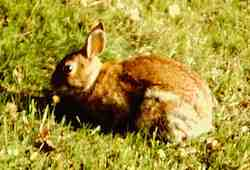
\includegraphics[width=\marginparwidth]{Matrices/rabbit}}%
\idx{Fibonacci} famously considered the breeding of \idx{rabbit}s---such as the following question.
One pair of rabbits can give birth to another pair of rabbits (called \idx{kitten}s) every month, say.
\begin{aside}
Fibonacci's real name is Leonardo Bonacci. 
He lived circa 1175 to 1250, travelled extensively from Pisa, and is considered to be one of the most talented Western mathematicians of the Middle Ages.
\end{aside}%
Each \idx{kitten} becomes fertile after it has aged a month, when it becomes \idx{adult} and is called a buck (male) or doe (\idx{female}).
The new bucks and does then also start breeding.
How many rabbits are there after six months?

Let's count just the females, the does, and the female kittens.
At the start of any month let there be \(x_1\)~kittens (female) and \(x_2\)~does.
Then at the end of the month:
\begin{itemize}
\item because all the female kittens grow up to be does, the number of does is now \(x_2'=x_2+x_1\)\,;
\item and because all the does at the start month have bred another pair of kittens, of which we expect one to be female, the new number of female kittens just born is \(x_1'=x_2\)\,.
\end{itemize}
Then \(x_1'\) and~\(x_2'\) is the number of kittens and does at the start of the next month.
Write this as a matrix vector system.
Let the female population be \(\xv=(x_1,x_2)\) and the population one month later be \(\xv'=(x_1',x_2')\).
Then our model is that
\begin{equation*}
\xv'=\begin{bmatrix} x_1'\\x_2' \end{bmatrix}
=\begin{bmatrix} x_2\\x_1+x_2 \end{bmatrix}
=\begin{bmatrix} 0&1\\1&1 \end{bmatrix}\begin{bmatrix} x_1\\x_2 \end{bmatrix}
=L\xv
\quad\text{for }L=\begin{bmatrix} 0&1\\1&1 \end{bmatrix},
\end{equation*}
called a \idx{Leslie matrix}.
\marginpar{Named after Patrick~H. Leslie, Leslie matrices are widely used in ecology to model the evolution over time of a population of organisms.}
\begin{itemize}
\item At the start there is one adult pair, one doe, and no female kittens, so the \idx{initial population} is \(\xv=(0,1)\).
\item After one month,  females \(\xv'=L\xv=\begin{bmat} 0&1\\1&1 \end{bmat}\begin{bmat} 0\\1 \end{bmat}=\begin{bmat} 1\\1 \end{bmat}\).
\item After two months,  females \(\xv''=L\xv'=\begin{bmat} 0&1\\1&1 \end{bmat}\begin{bmat} 1\\1 \end{bmat}=\begin{bmat} 1\\2 \end{bmat}\).
\item After three months,  females \(\xv'''=L\xv''=\begin{bmat} 0&1\\1&1 \end{bmat}\begin{bmat} 1\\2 \end{bmat}=\begin{bmat} 2\\3 \end{bmat}\).
\item After four months,  females \(\xv^{iv}=L\xv'''=\begin{bmat} 0&1\\1&1 \end{bmat}\begin{bmat} 2\\3 \end{bmat}=\begin{bmat} 3\\5 \end{bmat}\).
\item After five months,  females \(\xv^{v}=L\xv^{iv}=\begin{bmat} 0&1\\1&1 \end{bmat}\begin{bmat} 3\\5 \end{bmat}=\begin{bmat} 5\\8 \end{bmat}\).
\item After six months,  females \(\xv^{vi}=L\xv^{v}=\begin{bmat} 0&1\\1&1 \end{bmat}\begin{bmat} 5\\8 \end{bmat}=\begin{bmat} 8\\13 \end{bmat}\).
\end{itemize}
Fibonacci's model predicts the rabbit population grows rapidly according to the famous \idx{Fibonacci numbers} \(\mathcode`\,="213B 1,2,3,5,8,13,21,34,55,89,\ldots\)\,.
\end{example}
\end{reduce}



\begin{example}[\idx{age structured population}] \label{eg:matasp}
% adapted from SACE Math Studies 2012
An ecologist studies an isolated population of a \idx{species} of animal.
The growth of the population depends primarily upon the females so it is only these that are counted.
The females are grouped into three ages: female \idx{pup}s (in their first year), \idx{juvenile} females (one year old), and \idx{adult} females (two years or older).
During the study, the ecologist observes the following happens over the period of a year:
\begin{itemize}
\item  half of the female pups survive and become juvenile females;
\item  one-third of the juvenile females survive and become adult females;
\item  each adult female breeds and produces four female pups;
\item  one-third of the adult females survive to breed in the following year;
\item  female pups and juvenile females do not breed.
\end{itemize}
\begin{enumerate}
\item Let \(x_1\), \(x_2\) and~\(x_3\) be the number of females at the start of a year, of ages zero, one and two+ respectively, and let \(x'_1\), \(x'_2\) and~\(x'_3\) be their number at the start of the next year.
Use the ecologist's observations to write \(x'_1\), \(x'_2\) and~\(x'_3\) as a function of \(x_1\), \(x_2\) and~\(x_3\)  (this function is called a \idx{Markov chain}).
\item Letting vectors \(\xv=(x_1,x_2,x_3)\) and \(\xv'=(x'_1,x'_2,x'_3)\) write down your function as the matrix-vector product \(\xv'=L\xv\) for some matrix~\(L\) (called a \idx{Leslie matrix}).
\item Suppose the ecologist observes the numbers of females at the start of a given year is \(\xv=(60,70,20)\), use your matrix to predict the numbers~\(\xv'\) at the start of the next year.  
Continue similarly to predict the numbers after two years~(\(\xv''\))? and three years~(\(\xv'''\))?
\end{enumerate}

\begin{solution} 
\begin{enumerate}
\item Since adult females breed and produce four female pups, \(x'_1=4x_3\)\,.
Since half of the female pups survive and become juvenile females, \(x'_2=\frac12x_1\)\,.
Since one-third of the juvenile females survive and become adult females, \(\frac13x_2\)~contributes to~\(x'_3\), but additionally one-third of the adult females survive to breed in the following year, so  \(x'_3=\frac13x_2+\frac13x_3\)\,.

\item Writing these equations into vector form
\begin{equation*}
\xv'=\begin{bmatrix} x'_1\\x'_2\\x'_3 \end{bmatrix}
=\begin{bmatrix} 4x_3\\\frac12x_1\\\frac13x_2+\frac13x_3 \end{bmatrix}
=\underbrace{\begin{bmatrix} 0&0&4\\\frac12&0&0\\0&\frac13&\frac13 \end{bmatrix}}_L\xv\,.
\end{equation*}

\item Given the initial numbers of female animals is \(\xv=(60,70,20)\), the number of females after one year is then predicted by the matrix-vector product 
\begin{equation*}
\xv'=L\xv=\begin{bmatrix} 0&0&4\\\frac12&0&0\\0&\frac13&\frac13 \end{bmatrix}
\begin{bmatrix} 60\\70\\20 \end{bmatrix}
=\begin{bmatrix} 80\\30\\30 \end{bmatrix}.
\end{equation*}
That is, the predicted numbers of females are \(80\)~pups, \(30\)~juveniles, and \(30\)~adults.

After a second year the number of females is then predicted by the matrix-vector product \(\xv''=L\xv'\).  Here
\begin{equation*}
\xv''=L\xv'=\begin{bmatrix} 0&0&4\\\frac12&0&0\\0&\frac13&\frac13 \end{bmatrix}\begin{bmatrix} 80\\30\\30 \end{bmatrix}
=\begin{bmatrix} 120\\40\\20 \end{bmatrix}.
\end{equation*}
After a third year the number of females is predicted by the matrix-vector product \(\xv'''=L\xv''\).  Here
\begin{equation*}
\xv'''=L\xv''=\begin{bmatrix} 0&0&4\\\frac12&0&0\\0&\frac13&\frac13 \end{bmatrix}\begin{bmatrix} 120\\40\\20 \end{bmatrix}
=\begin{bmatrix} 80\\60\\20 \end{bmatrix}.
\end{equation*}
\end{enumerate}
\end{solution}
\end{example}


\index{matrix-vector product|)}





\subsubsection{Matrix-matrix multiplication}
\index{matrix product|(}

Matrix-vector multiplication explicitly uses the vector in its equivalent form as an \(n\times1\) matrix---a matrix with one column.
Such multiplication immediately generalizes to the case of a right-hand matrix with multiple columns.

\begin{example} 
Let two matrices
\begin{equation*}
A=\begin{bmatrix} 3 & 2\\ -2 & 1 \end{bmatrix},\quad
B=\begin{bmatrix} 5 & -6 & 4\\ -1 & -3 & -3 \end{bmatrix},
\end{equation*}
then the matrix multiplication~\(AB\) may be done as the matrix~\(A\) multiplying each of the three columns in~\(B\).
That is, in detail write
\begin{eqnarray*}
AB&=&A\begin{bmatrix} 5 & -6 & 4\\ -1 & -3 & -3 \end{bmatrix}
\\&=&A\begin{bmatrix} 5 \V -6 \V 4\\ -1 \V -3 \V -3 \end{bmatrix}
\\&=&\begin{bmatrix} A\begin{bmatrix} 5\\-1 \end{bmatrix} \W
A\begin{bmatrix} -6\\-3 \end{bmatrix} \W
A\begin{bmatrix} 4\\-3 \end{bmatrix} \end{bmatrix}
\\&=&\begin{bmatrix} \begin{bmatrix} 13\\-11 \end{bmatrix} \W
\begin{bmatrix} -24\\9 \end{bmatrix} \W
\begin{bmatrix}6\\-11 \end{bmatrix} \end{bmatrix}
\\&=&\begin{bmatrix}  13& -24&6\\-11 &9&-11\end{bmatrix}.
\end{eqnarray*}
Conversely, the product~\(BA\) cannot be done because if we try the same procedure then
\begin{eqnarray*}
BA&=&B\begin{bmatrix} 3 & 2\\ -2 & 1 \end{bmatrix}
\\&=&B\begin{bmatrix} \begin{bmatrix} 3 \\ -2 \end{bmatrix}\W 
\begin{bmatrix} 2 \\ 1 \end{bmatrix} \end{bmatrix}
\\&=&\begin{bmatrix} B\begin{bmatrix} 3 \\ -2 \end{bmatrix}\W 
B\begin{bmatrix} 2 \\ 1 \end{bmatrix} \end{bmatrix},
\end{eqnarray*}
and neither of these matrix-vector products can be done as, for example,
\begin{equation*}
B\begin{bmatrix} 3 \\ -2 \end{bmatrix}
=\begin{bmatrix} 5 & -6 & 4\\ -1 & -3 & -3 \end{bmatrix}
\begin{bmatrix} 3 \\ -2 \end{bmatrix}
\end{equation*}
the number of columns of the left matrix is not equal to the number of elements of the vector on the right.
Hence the product~\(BA\) is not defined.
\end{example}




\begin{example} 
Let matrices
\begin{equation*}
C=\begin{bmatrix} -4 & -1\\ -4 & -1\\ 1 & 4 \end{bmatrix},\quad
D=\begin{bmatrix} -2 & -1 & -3\\ 1 & 3 & 0 \end{bmatrix}.
\end{equation*}
Compute, if possible, \(CD\) and~\(DC\); compare these products.
\begin{solution} 
\begin{itemize}
\item On the one hand,
\begin{eqnarray*}
CD&=&C\begin{bmatrix} -2 & -1 & -3\\ 1 & 3 & 0 \end{bmatrix}
\\&=&\begin{bmatrix} C\begin{bmatrix} -2\\1 \end{bmatrix}\W
C\begin{bmatrix} -1\\3 \end{bmatrix}\W
C\begin{bmatrix} -3\\0 \end{bmatrix}
 \end{bmatrix}
\\&=&\begin{bmatrix} 7&1&12\\7&1&12\\2&11&-3 \end{bmatrix}.
\end{eqnarray*}

\item Conversely,
\begin{eqnarray*}
DC&=&D\begin{bmatrix} -4 & -1\\ -4 & -1\\ 1 & 4 \end{bmatrix}
\\&=&\begin{bmatrix}  D\begin{bmatrix} -4\\-4\\1 \end{bmatrix}\W
D\begin{bmatrix} -1\\-1\\4 \end{bmatrix}
\end{bmatrix}
\\&=&\begin{bmatrix} 9&-9\\-16&-4 \end{bmatrix}.
\end{eqnarray*}
\end{itemize}
Interestingly, \(CD\neq DC\)\,---they are not even of the same size!
\end{solution}
\end{example}


\begin{definition}[matrix product] \label{def:matprod}
  Let matrix~\(A\) be \(m\times n\), and matrix \(B\) be \(n\times 
  p\), then the \bfidx{matrix product} \(C=AB\), or 
  \bfidx{matrix multiplication}, is the \(m\times p\) matrix whose \((i,j)\)th~entry is
\begin{equation*}
c_{ij}=a_{i1}b_{1j}+a_{i2}b_{2j}+\cdots+a_{in}b_{nj}\,.
\end{equation*}
\end{definition}

This formula looks like a \idx{dot product}~(\autoref{def:dotprod}) of two vectors: indeed we do use that the expression for the \((i,j)\)th~entry is the dot product of the \(i\)th~row of~\(A\) and the \(j\)th~column of~\(B\) as illustrated by
\begin{equation*}
\begin{bmatrix} a_{11}&a_{12}&\cdots&a_{1n}
\\\vdots&\vdots&&\vdots
\\\rlap{\color{blue}\hspace{-0.2em}\framebox{\phantom{\rule{8.7em}{1ex}}}}
a_{i1}&a_{i2}&\cdots&a_{in}
\\\vdots&\vdots&&\vdots
\\a_{m1}&a_{m2}&\cdots&a_{mn} \end{bmatrix}
\begin{bmatrix} b_{11}&\cdots&b_{1j}&\cdots&b_{1p}
\\b_{21}&\cdots&b_{2j}&\cdots&b_{2p}
\\\vdots&&\vdots&&\vdots
\\b_{n1}&\cdots&
\rlap{\color{blue}\hspace{-0.25em}\smash{\framebox{\phantom{\rule[-0.5ex]{1em}{12ex}}}}}
b_{nj}&\cdots&b_{np} \end{bmatrix}.
\end{equation*}
As seen in the examples, although the two matrices~\(A\) and~\(B\) may be of different sizes, the number of columns of~\(A\) must equal the number of rows of~\(B\) in order for the product~\(AB\) to be defined.




\begin{activity}
Which one of the following \idx{matrix product}s is not defined?
\actposs{\(\begin{bmatrix} 8&9&3
\\2&5&1 \end{bmatrix}\begin{bmatrix} -2&8
\\3&-2 \end{bmatrix}\)}
{\(\begin{bmatrix} -1&2
\\1&-3 \end{bmatrix}\begin{bmatrix} -3&-1&-1
\\0&-4&-1 \end{bmatrix}\)}
{\(\begin{bmatrix} 3&-1 \end{bmatrix}\begin{bmatrix} -3&1
\\7&-3 \end{bmatrix}\)}
{\(\begin{bmatrix} 2&5&-3 \end{bmatrix}\begin{bmatrix} -3&1
\\-5&-1
\\2&-2 \end{bmatrix}\)}
\end{activity}




\begin{example} 
Matrix multiplication leads to powers of a square matrix.
Let matrix
\begin{equation*}
A=\begin{bmatrix} 3&2\\-2&1 \end{bmatrix},
\end{equation*}
then by~\(A^2\) we mean the product
\begin{equation*}
AA=\begin{bmatrix} 3&2\\-2&1 \end{bmatrix}\begin{bmatrix} 3&2\\-2&1 \end{bmatrix}=\begin{bmatrix} 5&8\\-8&-3 \end{bmatrix},
\end{equation*}
and by~\(A^3\) we mean the product
\begin{equation*}
AAA=AA^2=\begin{bmatrix} 3&2\\-2&1 \end{bmatrix}
\begin{bmatrix} 5&8\\-8&-3 \end{bmatrix}
=\begin{bmatrix} -1&18\\-18&-19 \end{bmatrix},
\end{equation*}
and so on.
\end{example}

In general, for an \(n\times n\) square matrix~\(A\) and a positive integer exponent~\(p\) we define the \bfidx{matrix power}
\begin{equation*}
A^p=\underbrace{AA\cdots A}_{p\text{ factors}}.
\end{equation*}
The \idx{matrix power}s~\(A^p\) are also \(n\times n\) square matrices.


\begin{example}[\idx{age structured population}] \label{eg:poppred}
\index{matrix power}Matrix powers occur naturally in modelling populations by ecologists such as the animals of \autoref{eg:matasp}.
Recall that given the numbers of \idx{female} \idx{pup}s, \idx{juvenile}s and \idx{adult}s formed into a vector \(\xv=(x_1,x_2,x_3)\), the number in each age one year later (indicated here by a dash) is \(\xv'=L\xv\) for \idx{Leslie matrix}
\begin{equation*}
L=\begin{bmatrix} 0&0&4\\\frac12&0&0\\0&\frac13&\frac13 \end{bmatrix}.
\end{equation*}
Hence the number in each age category two years later (indicated here by two dashes) is
\begin{equation*}
\xv''=L\xv'=L(L\xv)=(LL)\xv=L^2\xv\,,
\end{equation*}
provided that matrix multiplication is associative (established by \autoref{thm:pmma}) to enable us to write \(L(L\xv)=(LL)\xv\)\,.
Then the matrix square
\begin{equation*}
L^2=\begin{bmatrix} 0&0&4\\\frac12&0&0\\0&\frac13&\frac13 \end{bmatrix}\begin{bmatrix} 0&0&4\\\frac12&0&0\\0&\frac13&\frac13 \end{bmatrix}
=\begin{bmatrix} 0&\frac43&\frac43\\0&0&2\\\frac16&\frac19&\frac19 \end{bmatrix}.
\end{equation*}
Continuing to use such associativity, 
the number in each age category three years later (indicated here by threes dashes) is
\begin{equation*}
\xv'''=L\xv''=L(L^2\xv)=(LL^2)\xv=L^3\xv\,,
\end{equation*}
where the matrix cube
\begin{equation*}
L^3=LL^2=\begin{bmatrix} 0&0&4\\\frac12&0&0\\0&\frac13&\frac13 \end{bmatrix}\begin{bmatrix} 0&\frac43&\frac43\\0&0&2\\\frac16&\frac19&\frac19 \end{bmatrix}
=\begin{bmatrix} \frac23&\frac49&\frac49\\ 0&\frac23&\frac23\\  \frac1{18}&\frac1{27}&\frac{19}{27}\end{bmatrix}.
\end{equation*}
That is, the powers of the Leslie matrix help predict what happens two, three, or more years into the future.
\end{example}

\index{matrix multiplication|)}
\index{matrix product|)}





\subsubsection{The transpose of a matrix}

\index{transpose|(}

The operations so far defined for matrices correspond directly to analogous operations for scalars.
The transpose has no corresponding analogue.
At first mysterious, the transpose occurs frequently---often due to it linking the dot product of vectors with matrix multiplication.
The transpose also reflects symmetry in applications (\autoref{ch:eesm}), such as Newton's law that every action has an equal and opposite reaction.

\begin{example} \label{eg:mattrans}
Let matrices
\begin{equation*}
A=\begin{bmatrix} -4 & 2\\ -3 & 4\\ -1 & -7 \end{bmatrix},\quad
B=\begin{bmatrix} 2 & 0 & -1 \end{bmatrix},\quad
C=\begin{bmatrix} 1 & 1 & 1\\ -1 & -3 & 0\\ 2 & 3 & 2 \end{bmatrix}.
\end{equation*}
Then obtain the transpose of each of these three matrices by writing each of their rows as columns, in order:
\begin{equation*}
\tr A=\begin{bmatrix} -4 & -3 & -1\\ 2 & 4 & -7 \end{bmatrix},\quad
\tr B=\begin{bmatrix} 2\\ 0\\ -1 \end{bmatrix},\quad
\tr C=\begin{bmatrix} 1 & -1 & 2\\ 1 & -3 & 3\\ 1 & 0 & 2 \end{bmatrix}.
\end{equation*}
\end{example}

These examples illustrate the following definition. 
\begin{definition}[transpose] \label{def:mattran}
The \bfidx{transpose} of an \(m\times n\) matrix~\(A\) is the \(n\times m\) matrix, denoted~\(\tr A\), obtained by writing the \(i\)th~row of~\(A\) as the \(i\)th~column of~\(\tr A\), or equivalently by writing the \(j\)th~column of~\(A\) to be the \(j\)th~row of~\(\tr A\).
That is, if \(B=\tr A\), then \(b_{ij}=a_{ji}\).
\end{definition}



\begin{activity}
Which of the following matrices is the transpose of the matrix
\begin{equation*}
\begin{bmatrix} 1&-0.5&2.9
\\-1.4&-1.4&-0.2
\\0.9&-2.3&1.6 \end{bmatrix}?
\end{equation*}
\actposs{\(\begin{bmatrix} 1&-1.4&0.9
\\-0.5&-1.4&-2.3
\\2.9&-0.2&1.6 \end{bmatrix}\)}
{\(\begin{bmatrix} 0.9&-2.3&1.6
\\-1.4&-1.4&-0.2
\\1&-0.5&2.9 \end{bmatrix}\)}
{\(\begin{bmatrix} 2.9&-0.5&1
\\-0.2&-1.4&-1.4
\\1.6&-2.3&0.9 \end{bmatrix}\)}
{\(\begin{bmatrix} 1.6&-2.3&0.9
\\-0.2&-1.4&-1.4
\\2.9&-0.5&1 \end{bmatrix}\)}
\end{activity} 




\begin{example}[transpose and \idx{dot product}] \label{eg:trdp}
Consider two vectors in~\(\RR^n\), say \(\uv=(\hlist un)\) and \(\vv=(\hlist vn)\); that is,
\begin{equation*}
\uv=\begin{bmatrix} u_1\\u_2\\\vdots\\u_n \end{bmatrix},\quad
\vv=\begin{bmatrix} v_1\\v_2\\\vdots\\v_n \end{bmatrix}.
\end{equation*}
Then the dot product between the two vectors
\begin{eqnarray*}
\uv\cdot\vv&=&u_1v_1+u_2v_2+\cdots+u_nv_n \quad(\text{\autoref{def:dotprod} of dot})
\\&=&\begin{bmatrix} u_1&u_2&\cdots&u_n \end{bmatrix}
\begin{bmatrix} v_1\\v_2\\\vdots\\v_n \end{bmatrix}\quad(\text{\autoref{def:matprod} of mult.})
\\&=&\tr{\begin{bmatrix} u_1\\u_2\\\vdots\\u_n \end{bmatrix}}
\begin{bmatrix} v_1\\v_2\\\vdots\\v_n \end{bmatrix}\quad(\text{transpose \autoref{def:mattran}})
\\&=&\tr{\uv}\vv\,.
\end{eqnarray*}
Subsequent sections and chapters often use this identity, that the dot product \(\uv\cdot\vv=\tr{\uv}\vv\)\,.
\end{example}


\begin{definition}[symmetry] \label{def:matsym}
A (real) matrix~\(A\) is a \bfidx{symmetric matrix} if \(\tr A=A\)\,; that is, if the matrix is equal to its \idx{transpose}.
\end{definition}

A \idx{symmetric matrix} must be a square matrix---as otherwise the sizes of \(A\) and~\(\tr A\) would be different and so the matrices could not be equal.


\begin{example} 
None of the three matrices in \autoref{eg:mattrans} are symmetric: the first two matrices are not square so cannot be symmetric; and the third matrix \(C\neq\tr C\).  
The following matrix is symmetric:
\begin{equation*}
D=\begin{bmatrix} 2 & 0 & 1\\ 0 & -6 & 3\\ 1 & 3 & 4  \end{bmatrix}
=\tr D.
\end{equation*}
When is the following general \(2\times2\) matrix symmetric?
\begin{equation*}
E=\begin{bmatrix} a&b\\c&d \end{bmatrix}.
\end{equation*}
\begin{solution} 
Consider the transpose
\begin{equation*}
\tr E=\begin{bmatrix} a&c\\b&d \end{bmatrix}
\quad\text{compared with }
E=\begin{bmatrix} a&b\\c&d \end{bmatrix}.
\end{equation*}
The top-left and bottom-right elements are always the same.
The top-right and bottom-left elements will be the same if and only if \(b=c\).
That is, the \(2\times 2\) matrix~\(E\) is symmetric if and only if \(b=c\)\,.
\end{solution}
\end{example}

Symmetric matrices of note are the \(n\times n\) \idx{identity matrix} and \(n\times n\) \idx{zero matrix}, \(I_n\) and~\(O_n\).


\begin{activity}
Which one of the following matrices is a \idx{symmetric matrix}?
\actposs{\(\begin{bmatrix} -2.6&0.3&-1.3
\\0.3&-0.2&0
\\-1.3&0&-2 \end{bmatrix}\)}
{\(\begin{bmatrix} 0&-3.2&-0.8
\\3.2&0&3.2
\\0.8&-3.2&0 \end{bmatrix}\)}
{\(\begin{bmatrix} 2.3&-1.3&-2
\\-3.2&-1&-1.3
\\-3&-3.2&2.3 \end{bmatrix}\)}
{\(\begin{bmatrix} 2.2&-0.9&-1.2
\\-0.9&-1.2&-3.1 \end{bmatrix}\)}
\end{activity}
   


\index{transpose|)}






\subsubsection{Compute in \script}

\script\ empowers us to compute all these operations quickly, especially for the large problems found in applications: after all, \script[1]\ is an abbreviation of \emph{Mat}rix \emph{Lab}oratory.
\autoref{tbl:mtlbops} summarizes the \script\ version of the operations introduced so far, and used in the rest of this book.

\begin{table}
\caption{As well as the basics of \script\ listed in \autoref{tbl:mtlbpre,tbl:mtlbbasics},  we need these matrix operations.\index{Matlab@\textsc{Matlab}|textbf}\index{Octave|textbf}} \label{tbl:mtlbops}
\hrule
\begin{minipage}{\linewidth}
\begin{itemize}
\item \index{size()@\texttt{size()}|textbf}\verb|size(A)| returns the number of rows and columns of matrix~\(A\): if \(A\) is \(m\times n\), then \verb|size(A)| returns \(\begin{bmatrix} m&n \end{bmatrix}\).
\item \verb|A(i,j)| is the \((i,j)\)th entry of a matrix~\(A\), \verb|A(:,j)|~is the \(j\)th~column, \verb|A(i,:)|~is the \(i\)th~row; either to use the value(s) or to assign value(s).
\item \index{+,-,*@\texttt{+,-,*}|textbf}\verb|+,-,*| is matrix\slash vector\slash scalar addition, \idx{subtraction}, and multiplication, but only provided the sizes of the two operands are compatible.
%\item As well as enclosing subscripts, parentheses,~\verb|()|, control the order of evaluation of a complicated expression.
\item \verb|A^p| for scalar~\(p\) computes the \(p\)th~power of square matrix~\(A\) (in contrast to~\verb|A.^p| which  computes the \(p\)th~power of \emph{each element} of~\(A\), \autoref{tbl:mtlbbasics}).
\item The character single \bfidx{quote},~\verb|A'|, \idx{transpose}s the matrix~\(A\).  
But when using \idx{complex number}s be wary: \verb|A'|~is the \idx{complex conjugate} transpose (which is what we usually want); whereas \verb|A.'|~is the transpose without complex conjugation.
\item Predefined matrices include:
\begin{itemize}
\item \index{zero matrix|textbf}\index{zeros()@\texttt{zeros()}|textbf}\verb|zeros(m,n)| is the \idx{zero matrix}~\(O_{m\times n}\);
\item \index{eye()@\texttt{eye()}|textbf}\verb|eye(m,n)|~is \(m\times n\) `\idx{identity matrix}'~\(I_{m\times n}\);
\item \index{ones matrix|textbf}\index{ones()@\texttt{ones()}|textbf}\verb|ones(m,n)| is the \(m\times n\) matrix where all \idx{entries} are one;
\item \index{random matrix|textbf}\index{randn()@\texttt{randn()}|textbf}\verb|randn(m,n)|~is a \(m\times n\) matrix with \idx{random entries} (independent, distributed Normally, \idx{mean} zero, \idx{standard deviation} one).
\end{itemize}
A single argument gives the \idx{square matrix} version: 
\begin{itemize}
\item \index{zero matrix|textbf}\verb|zeros(n)| is~\(O_n=O_{n\times n}\); 
\item \verb|eye(n)|~is the \(n\times n\) \idx{identity matrix} \(I_n=I_{n\times n}\);  
\item \verb|ones(n)| is the \(n\times n\) matrix of all ones;
\item \index{random matrix|textbf}\verb|randn(n)|~is an \(n\times n\) matrix with \idx{random entries}.
\end{itemize}
With no argument, these functions return the corresponding scalar: for example, \verb|randn|~computes a single random number.
\item Very large and small magnitude numbers are printed in \script\ like the following: 
\begin{itemize}
\item \verb|4.852e+08| denotes the large \(4.852\cdot10^8\); whereas 
\item \verb|3.469e-16| denotes the small \(3.469\cdot10^{-16}\).
\end{itemize}
\end{itemize}
\end{minipage}
\hrule
\end{table}

\paragraph{Matrix size and elements}
\index{size}\index{size()@\texttt{size()}}
Let the matrix
\begin{equation*}
A=\begin{bmatrix} 0 & 0 & -2 & -11 & 5\\ 0 & 1 & -1 & 11 & -8\\ -4 & 2 & 10 & 2 & -3 \end{bmatrix}.
\end{equation*}
We readily see this is a \(3\times5\) matrix, but to check that \script\ agrees, execute the following in \script: \index{size}
\begin{verbatim}
A=[0 0 -2 -11  5
   0 1 -1  11 -8
  -4 2 10   2 -3]
size(A)
\end{verbatim}
\setbox\ajrqrbox\hbox{\qrcode{% matrix elements
A=[0 0 -2 -11  5
   0 1 -1  11 -8
  -4 2 10   2 -3]
size(A)
A(2,4)
A(:,5)
A(1,:)
A(2,4)=9
A(:,5)=[2;-3;1]
A(1,:)=[1 2 3 4 5]
}}%
\marginajrbox%
The answer, ``\verb|3  5|'', confirms \(A\) is \(3\times5\).
\script\ accesses individual \idx{elements}, rows and columns.
For example, execute each of the following:
\begin{itemize}
\item \verb|A(2,4)| gives~\(a_{24}\) which here results in~\(11\);
\item \verb|A(:,5)| is the fifth \idx{column vector}, here \(\begin{bmatrix} 5\\ -8\\ -3 \end{bmatrix}\);
\item \verb|A(1,:)| is the first row, here \(\begin{bmatrix} 0 & 0 & -2 & -11 & 5 \end{bmatrix}\).
\end{itemize}
One may also use these constructs to change the elements in matrix~\(A\): for example, executing
\verb|A(2,4)=9| changes matrix~\(A\) to
\begin{verbatim}
A =
     0     0    -2   -11     5
     0     1    -1     9    -8
    -4     2    10     2    -3
\end{verbatim}
then \verb|A(:,5)=[2;-3;1]| changes matrix~\(A\) to
\begin{verbatim}
A =
     0     0    -2   -11     2
     0     1    -1     9    -3
    -4     2    10     2     1
\end{verbatim}
whereas \verb|A(1,:)=[1 2 3 4 5]| changes matrix~\(A\) to
\begin{verbatim}
A =
     1     2     3     4     5
     0     1    -1     9    -3
    -4     2    10     2     1
\end{verbatim}


\paragraph{Matrix addition and subtraction}
To illustrate further operations let's use some random matrices generated by \script: you will generate different matrices to the following, but the operations will work the same.
\autoref{tbl:mtlbops} mentions that \verb|randn(m)| and \verb|randn(m,n)| generate random matrices so execute say
\begin{verbatim}
A=randn(4)
B=randn(4)
C=randn(4,2)
\end{verbatim}
and obtain matrices such as \twodp
\setbox\ajrqrbox\hbox{\qrcode{% matrix add and subtract
A=randn(4)
B=randn(4)
C=randn(4,2)
A+B
A-B
(A+B)-(B+A)
B+C
}}%
\marginajrbox%
\begin{verbatim}
A =
  -1.31   2.07   0.08   2.05
   1.25  -1.35  -1.00   1.94
   1.08   1.79  -0.99   0.93
   1.34  -0.99  -0.23  -0.22
B =
   1.21  -0.46   0.09   0.58
   1.67  -1.96   1.26   1.93
   0.24  -0.46   2.77  -0.59
   0.03  -0.28  -0.76   0.13
C =
   1.14   0.85
  -0.48   0.17
   0.37  -0.64
   0.62  -1.17
\end{verbatim}
Then \verb|A+B| gives here the sum\index{addition}\index{sum}
\begin{verbatim}
ans =
  -0.10   1.62   0.17   2.63
   2.92  -3.31   0.26   3.87
   1.31   1.33   1.78   0.34
   1.37  -1.27  -0.99  -0.09
\end{verbatim}
and \verb|A-B| the difference\index{subtraction}\index{difference}
\begin{verbatim}
ans =
  -2.52   2.53  -0.01   1.46
  -0.41   0.62  -2.25   0.01
   0.84   2.26  -3.76   1.52
   1.31  -0.71   0.53  -0.35
\end{verbatim}
You could check that \verb|B+A| gives the same matrix as \verb|A+B| (\autoref{thm:pasma}) by seeing that their \idx{difference} is the \(4\times4\) zero matrix: execute \verb|(A+B)-(B+A)| (the parentheses control the order of evaluation).
However, expressions such as \verb|B+C| and \verb|A-C| give an error, because the matrices are of incompatible sizes, reported by \script[1]\ as\index{Error using@\texttt{Error using}}%
\index{nonconformant arguments@\texttt{nonconformant arguments}}%
\index{dimensions must agree@\texttt{dimensions must agree}}%
\begin{verbatim}
Error using  + 
Matrix dimensions must agree. 
\end{verbatim}
or reported by Octave as\index{error:@\texttt{error:}}
\begin{verbatim}
error: operator +: nonconformant arguments 
\end{verbatim}


\paragraph{Scalar multiplication of matrices}
In \script\ the asterisk indicates multiplication.
Scalar multiplication can be done either way around.
For example, generate a random \(4\times 3\) matrix~\(A\) and compute \(2A\) and~\(A\frac1{10}\).
These commands 
\begin{verbatim}
A=randn(4,3)
2*A
A*0.1
\end{verbatim}
\setbox\ajrqrbox\hbox{\qrcode{% scalar multiplication et al
A=randn(4,3)
2*A
A*0.1
A+3
2*A-5
}}%
\marginajrbox%
might give the following \twodp
\begin{verbatim}
A =
   0.82   2.54  -0.98
   2.30   0.05   2.63
  -1.45   2.15   0.89
  -2.58  -0.09  -0.55

>> 2*A
ans =
   1.64   5.07  -1.97
   4.61   0.10   5.25
  -2.90   4.30   1.77
  -5.16  -0.18  -1.11

>> A*0.1
ans =
   0.08   0.25  -0.10
   0.23   0.00   0.26
  -0.15   0.21   0.09
  -0.26  -0.01  -0.06
\end{verbatim}
Division by a scalar is also defined in \script\ and means multiplication by the reciprocal; for example, the product~\verb|A*0.1| could equally well be computed as~\verb|A/10|.

In mathematical algebra we would not normally accept statements such as \(A+3\) or \(2A-5\) because addition and subtraction with matrices has only been defined between matrices of the same size.\footnote{Although in some contexts such mathematical expressions are routinely accepted, be careful of their meaning.}
However, \script\ usefully extends addition and subtraction so that \verb|A+3| and \verb|2*A-5| mean add three to \emph{every} element of~\(A\) and subtract five from \emph{every} element of~\(2A\). 
For example, with the above random \(4\times3\) matrix~\(A\),
\begin{verbatim}
>> A+3
ans =
   3.82   5.54   2.02
   5.30   3.05   5.63
   1.55   5.15   3.89
   0.42   2.91   2.45

>> 2*A-5
ans =
   -3.36    0.07   -6.97
   -0.39   -4.90    0.25
   -7.90   -0.70   -3.23
  -10.16   -5.18   -6.11
\end{verbatim}
This last computation illustrates that in any expression the operations of multiplication and division are performed before additions and subtractions---as normal in mathematics.


\paragraph{Matrix multiplication}
In \script\ the asterisk also invokes matrix-matrix and matrix-vector multiplication.
For example, generate and multiply two random matrices say of size \(3\times4\) and \(4\times 2\) with 
\begin{verbatim}
A=randn(3,4)
B=randn(4,2)
C=A*B
\end{verbatim}
\setbox\ajrqrbox\hbox{\qrcode{% scalar multiplication et al
A=randn(3,4)
B=randn(4,2)
C=A*B
A(1,:)*B(:,1)
[A*B(:,1) A*B(:,2)]
B*A
}}%
\marginajrbox%
might give the following result \twodp\ 
\begin{verbatim}
A =
  -0.02   1.31  -0.74  -0.49
  -0.36  -1.30  -0.23   0.41
  -0.88  -0.34   0.28  -0.99

B =
  -1.32  -0.79
   0.71   1.48
  -0.48   2.79
   1.40  -0.41

>> C=A*B
C =
   0.62   0.10
   0.24  -2.44
  -0.60   1.38
\end{verbatim}
Without going into excruciating arithmetic detail this product is hard to check.
However, we can check several things such as \(c_{11}\) comes from the first row of~\(A\) times the first column of~\(B\) by computing \verb|A(1,:)*B(:,1)| and seeing it does give~\(0.62\) as required.
Also check that the two columns of~\(C\) may be viewed as the two \idx{matrix-vector product}s \(A\bv_1\) and~\(A\bv_2\) by comparing~\(C\) with \verb|[A*B(:,1) A*B(:,2)]| and seeing they are the same.

Recall that in a \idx{matrix product} the number of columns of the left matrix have to be the same as the number of rows of the right matrix.
\script\ gives an error message if this is not the case, such as occurs  upon asking it to compute~\verb|B*A| when \script[1] reports
\index{Error using@\texttt{Error using}}%
\index{nonconformant arguments@\texttt{nonconformant arguments}}%
\index{dimensions must agree@\texttt{dimensions must agree}}%
\begin{verbatim}
Error using  * 
Inner matrix dimensions must agree.
\end{verbatim}
and \script[2] reports\index{error:@\texttt{error:}}
\begin{verbatim}
error: operator *: nonconformant arguments
\end{verbatim}

The caret symbol,~\verb|^|, computes \idx{matrix power}s in \script, such as the cube~\verb|A^3|. 
But such matrix powers only makes sense and works for square matrices~\(A\).%
\footnote{Here we define matrix powers for only integer power. \script\ will compute the power of a square matrix for any real\slash complex exponent, but its meaning involves matrix exponentials and logarithms that we do not explore here.}
For example, if matrix~\(A\) was \(3\times4\)\,, then \(A^2=AA\) would involve multiplying a \(3\times4\) matrix by a \(3\times4\) matrix: since the number of columns of the left~\(A\) is not the same as the number of rows of the right~\(A\) such a multiplication is not allowed.



\paragraph{The transpose and symmetry}
In \script\ the single apostrophe denotes matrix \idx{transpose}.
For example, see it transpose a couple of random matrices with
\begin{verbatim}
A=randn(3,4)
B=randn(4,2)
A'
B'
\end{verbatim}
\setbox\ajrqrbox\hbox{\qrcode{% scalar multiplication et al
A=randn(3,4)
B=randn(4,2)
A'
B'
(A*B)'-B'*A'
C=randn(3)
C=C+C'
C-C'
}}%
\marginajrbox%
giving here for example \twodp
\begin{verbatim}
A =
   0.80   0.30  -0.12  -0.57
   0.07  -0.51  -0.81   1.95
   0.29  -0.10   0.17   0.70
B =
  -0.71  -0.34
  -0.33  -0.73
   1.11  -0.21
   0.41   0.33

>> A'
ans =
   0.80   0.07   0.29
   0.30  -0.51  -0.10
  -0.12  -0.81   0.17
  -0.57   1.95   0.70

>> B'
ans =
  -0.71  -0.33   1.11   0.41
  -0.34  -0.73  -0.21   0.33
\end{verbatim}
One can do further operations after the transposition, such as checking the multiplication rule that \(\tr{(AB)}=\tr B\tr A\) (\autoref{thm:potd}) by verifying the result of \verb|(A*B)'-B'*A'| is the zero matrix, here~\(O_{2\times3}\).

You can generate a symmetric matrix by adding a square matrix to its transpose (\autoref{thm:potf}): for example, generate a random square matrix by first \verb|C=randn(3)| then \verb|C=C+C'| makes a random \idx{symmetric matrix} such as the following \twodp
\begin{verbatim}
>> C=randn(3)
C =
  -0.33   0.65  -0.62
  -0.43  -2.18  -0.28
   1.86  -1.00  -0.52

>> C=C+C'
C =
  -0.65   0.22   1.24
   0.22  -4.36  -1.28
   1.24  -1.28  -1.04

>> C-C'
ans =
   0.00   0.00   0.00
   0.00   0.00   0.00
   0.00   0.00   0.00
\end{verbatim}
That the resulting matrix~\(C\) is symmetric is checked by this last step which computes the \idx{difference} between~\(C\) and~\(\tr C\) and confirming the difference is zero. 
Hence \(C\) and~\(\tr C\) must be equal.






\subsection{Familiar algebraic properties of matrix operations}
\label{sec:fapmo}

Almost all of the familiar algebraic properties of scalar addition, 
subtraction and multiplication---namely \idx{commutativity}, \idx{associativity} and \idx{distributivity}---hold for matrix addition, subtraction and multiplication.

The one outstanding exception is that \idx{matrix multiplication} is \emph{not} commutative: for matrices~\(A\) and~\(B\) the products~\(AB\) and~\(BA\) are usually not equal.
We are used to such \idx{non-commutativity} in life.
For example, when you go home, to enter your house you first open the door, second walk in, and third close the door. 
You cannot swap the order and try to walk in before opening the door---these operations do not commute.
Similarly, for another example, I often teach classes on the third floor of a building next to my office: after finishing classes, first I walk downstairs to ground level, and second I cross the road to my office.
If I try to cross the road before going downstairs, then the force of gravity has something very painful to say about the outcome---the operations do not commute.
Similar to these analogues, the result of a matrix multiplication depends upon the order of the matrices in the multiplication.


\begin{theorem}[Properties of \idx{addition} and \idx{scalar multiplication}] \label{thm:pasm}
Let matrices \(A\), \(B\) and~\(C\) be of the same size, and let \(c\) and~\(d\) be scalars.  Then:
\begin{enumerate}[ref=\ref{thm:pasm}(\alph*)]
\item\label[theorem]{thm:pasma} \(A+B=B+A\) (\idx{commutativity} of addition);\index{commutative law}
\item \((A+B)+C=A+(B+C)\) (associativity of addition);\index{associative law}
\item \(A\pm O=A=O+A\);
\item \(c(A\pm B)=cA\pm cB\) (\idx{distributivity} over matrix addition);\index{distributive law}
\item \((c\pm d)A=cA\pm dA\) (\idx{distributivity} over scalar addition);\index{distributive law}
\item \(c(dA)=(cd)A\) (associativity of scalar multiplication);\index{associative law}
\item \(1A=A\)\,; and 
\item \(0A=O\)\,.
\end{enumerate}
\end{theorem}

\begin{proof}
The proofs directly match those of the corresponding vector properties and are set as exercises.
\end{proof}



\begin{example}[geometry of associativity]
Many properties of \idx{matrix multiplication} have a useful geometric interpretation such as that discussed for matrix-vector products.
Recall the earlier \autoref{eg:poppred} invoked the associativity \autoref{thm:pmma}.
For another example, consider the two matrices and vector
\begin{equation*}
A=\begin{bmatrix} 1&1\\1&0 \end{bmatrix},\quad
B=\begin{bmatrix} 2&0\\2&-1 \end{bmatrix},\quad
\xv=\begin{bmatrix} 1\\1 \end{bmatrix}.
\end{equation*}
\marginpar{\begin{tikzpicture}
\begin{axis}[footnotesize,width=12em
    , axis equal image, axis lines=middle,
    , grid,xmin=0,xmax=3.9,ymax=2.9 ]
    \addplot[blue,quiver={u=1,v=1},-stealth, thick] coordinates {(0,0)};
    \node[above] at (axis cs:1,1) {$\xv$};
    \addplot[red,quiver={u=2,v=1},-stealth, thick] coordinates {(0,0)};
    \node[below] at (axis cs:2,1) {$B\xv$};
    \addplot[brown,quiver={u=3,v=2},-stealth, thick] coordinates {(0,0)};
    \node[above] at (axis cs:3,2) {$A(B\xv)$};
\end{axis}
\end{tikzpicture}}%
Now the transform \(\xv'=B\xv=(2,1)\), and then transforming with~\(A\) gives \(\xv''=A\xv'=A(B\xv)=(3,2)\), as illustrated in the margin.
This is the same results as forming the product
\begin{equation*}
AB=\begin{bmatrix} 1&1\\1&0 \end{bmatrix} 
\begin{bmatrix} 2&0\\2&-1 \end{bmatrix}
=\begin{bmatrix} 4&-1\\2&0 \end{bmatrix}
\end{equation*}
and then computing \((AB)\xv=(3,2)\) as also illustrated in the margin.
\marginpar{\begin{tikzpicture}
\begin{axis}[footnotesize,width=12em
    , axis equal image, axis lines=middle,
    , grid,xmin=0,xmax=3.9,ymax=2.9 ]
    \addplot[blue,quiver={u=1,v=1},-stealth, thick] coordinates {(0,0)};
    \node[above] at (axis cs:1,1) {$\xv$};
%    \addplot[red,quiver={u=2,v=1},-stealth, thick] coordinates {(0,0)};
%    \node[below] at (axis cs:2,1) {$B\xv$};
    \addplot[brown,quiver={u=3,v=2},-stealth, thick] coordinates {(0,0)};
    \node[above] at (axis cs:3,2) {$(AB)\xv$};
\end{axis}
\end{tikzpicture}}%
Such associativity asserts that \(A(B\xv)=(AB)\xv\)\,: that is, the geometric transform of~\xv\ by matrix~\(B\) followed by the transform of matrix~\(A\) is the same result as just transforming by the matrix formed from the product~\(AB\)---as assured by \autoref{thm:pmma}.
\end{example}



\begin{theorem}[properties of \idx{matrix multiplication}] \label{thm:pmm}
Let matrices \(A\), \(B\) and~\(C\) be of sizes such that the following expressions are defined, and let \(c\)~be a \idx{scalar}, then:
\begin{enumerate}[ref=\ref{thm:pmm}(\alph*)]
\item\label[theorem]{thm:pmmb} \(A(B\pm C)=AB\pm AC\) (\idx{distributivity} of matrix multiplication);\index{distributive law}
\item\label[theorem]{thm:pmmbb} \((A\pm B)C=AC\pm BC\) (\idx{distributivity} of matrix multiplication);\index{distributive law}
\item\label[theorem]{thm:pmma} \(A(BC)=(AB)C\) (associativity of matrix multiplication);\index{associative law}
\item\label[theorem]{thm:pmmc} \(c(AB)=(cA)B=A(cB)\);
\item\label[theorem]{thm:pmmd} \(I_mA=A=AI_n\) for \(m\times n\) matrix~\(A\) (multiplicative identity);
\item\label[theorem]{thm:pmme} \(O_mA=O_{m\times n}=AO_n\)  for \(m\times n\) matrix~\(A\);
\item\label[theorem]{thm:pmmg} \(A^pA^q=A^{p+q}\), \((A^p)^q=A^{pq}\) and~\((cA)^p=c^pA^p\) for square matrices~\(A\) and for positive integers~\(p\) and~\(q\).\index{matrix power}%
\footnote{Generally these exponent properties hold for all scalar~\(p\) and~\(q\), although one has to be very careful with non-integer exponents.}
\end{enumerate}
\end{theorem}

\begin{proof} 
Let's document a few proofs, others are exercises.
\begin{description}
\item[\ref{thm:pmmb}]
This direct proof involves some long expressions involving the entries of \(m\times n\) matrix~\(A\), and \(n\times p\) matrices~\(B\) and~\(C\).
Let \((\cdot)_{ij}\) denote the \((i,j)\)th~entry of whatever matrix expression is inside the parentheses.
By \autoref{def:matprod} of matrix multiplication
\begin{align*}
&(A(B\pm C))_{ij}
\\&=a_{i1}(B\pm C)_{1j}+a_{i2}(B\pm C)_{2j}+\cdots+a_{in}(B\pm C)_{nj}
\\&\qquad(\text{then by definition of matrix addition})
\\&=a_{i1}(b_{1j}\pm c_{1j})+a_{i2}(b_{2j}\pm c_{2j})+\cdots+a_{in}(b_{nj}\pm c_{nj})
\\&\qquad(\text{then distributing the scalar multiplications})
\\&=a_{i1}b_{1j}\pm a_{i1}c_{1j}+a_{i2}b_{2j}\pm a_{i2}c_{2j}+\cdots+a_{in}b_{nj}\pm a_{in}c_{nj}
\\&\qquad(\text{then upon reordering terms in the sum})
\\&=a_{i1}b_{1j}+a_{i2}b_{2j}+\cdots+a_{in}b_{nj}
\\&\quad{}\pm (a_{i1}c_{1j}+ a_{i2}c_{2j}+\cdots +a_{in}c_{nj})
\\&\qquad(\text{then using \autoref{def:matprod} for matrix products})
\\&=(AB)_{ij} \pm (AC)_{ij}\,.
\end{align*}
Since this identity holds for all indices~\(i\) and~\(j\), the matrix identity \(A(B\pm C)=AB\pm AC\) holds, proving \autoref{thm:pmmb}.


\item[\ref{thm:pmma}] Associativity involves some longer expressions involving the entries of \(m\times n\) matrix~\(A\), \(n\times p\) matrix~\(B\), and \(p\times q\) matrix~\(C\). 
By \autoref{def:matprod} of matrix multiplication
\begin{eqnarray*}
%&\rlap{$(A(BC))_{ij}$}\\
(A(BC))_{ij}&=& a_{i1}(BC)_{1j}+a_{i2}(BC)_{2j}+\cdots+a_{in}(BC)_{nj}
\\&&\quad(\text{then using  \autoref{def:matprod} for }BC)
\\&=&\phantom{{}+{}}a_{i1}(b_{11}c_{1j}+b_{12}c_{2j}+\cdots+b_{1p}c_{pj})
\\&&{}+a_{i2}(b_{21}c_{1j}+b_{22}c_{2j}+\cdots+b_{2p}c_{pj})
\\&&{}+\cdots
\\&&{}+a_{in}(b_{n1}c_{1j}+b_{n2}c_{2j}+\cdots+b_{np}c_{pj})
\\&&{}\quad(\text{distributing the scalar multiplications})
\\&=&\phantom{{}+{}}a_{i1}b_{11}c_{1j}+a_{i1}b_{12}c_{2j}+\cdots+a_{i1}b_{1p}c_{pj}
\\&&{}+a_{i2}b_{21}c_{1j}+a_{i2}b_{22}c_{2j}+\cdots+a_{i2}b_{2p}c_{pj}
\\&&{}+\cdots
\\&&{}+a_{in}b_{n1}c_{1j}+a_{in}b_{n2}c_{2j}+\cdots+a_{in}b_{np}c_{pj}
\\&&{}\quad(\text{then reordering the terms---transpose})
\\&=&\phantom{{}+{}}a_{i1}b_{11}c_{1j}+a_{i2}b_{21}c_{1j}+\cdots+a_{in}b_{n1}c_{1j}
\\&&{}+a_{i1}b_{12}c_{2j}+a_{i2}b_{22}c_{2j}+\cdots+a_{in}b_{n2}c_{2j}
\\&&{}+\cdots
\\&&{}+a_{i1}b_{1p}c_{pj}+a_{i2}b_{2p}c_{pj}+\cdots+a_{in}b_{np}c_{pj}
\\&&{}\quad(\text{then factoring }c_{1j},c_{2j},\ldots c_{pj})
\\&=&\phantom{{}+{}}(a_{i1}b_{11}+a_{i2}b_{21}+\cdots+a_{in}b_{n1})c_{1j}
\\&&{}+(a_{i1}b_{12}+a_{i2}b_{22}+\cdots+a_{in}b_{n2})c_{2j}
\\&&{}+\cdots
\\&&{}+(a_{i1}b_{1p}+a_{i2}b_{2p}+\cdots+a_{in}b_{np})c_{pj}
\\&&{}\quad(\text{then recognizing the entries for }(AB)_{ik})
\\&=&(AB)_{i1}c_{1j} +(AB)_{i2}c_{2j} +\cdots +(AB)_{ip}c_{pj}
\\&&{}\quad(\text{then again using  \autoref{def:matprod}})
\\&=&((AB)C)_{ij}.
\end{eqnarray*}
Since this identity holds for all indices~\(i\) and~\(j\), the matrix identity \(A(BC)=(AB)C\) holds, proving \autoref{thm:pmma}.

\item[\ref{thm:pmmg}]
Other proofs develop from previous parts of the theorem.
For example, to establish \(A^pA^q=A^{p+q}\) start from the definition of matrix powers:
\begin{eqnarray*}
A^pA^q&=&(\underbrace{AA\cdots A}_{p\text{ times}})
(\underbrace{AA\cdots A}_{q\text{ times}})
\\&&\quad(\text{using associativity, \autoref{thm:pmma}})
\\&=&\underbrace{AA\cdots A}_{p+q\text{ times}}
\\&=&A^{p+q}.
\end{eqnarray*}

\end{description}
\end{proof}



\begin{example} 
Show that \((A+B)^2\neq A^2+2AB+B^2\)  in general.
\begin{solution} 
Consider
\begin{eqnarray*}
(A+B)^2&=& (A+B)(A+B) \quad(\text{matrix power})
\\&=&A(A+B)+B(A+B) \quad(\text{\autoref{thm:pmmbb}})
\\&=&AA+AB+BA+BB \quad(\text{\autoref{thm:pmmb}})
\\&=&A^2+AB+BA+B^2 \quad(\text{matrix power}).
\end{eqnarray*}
This expression is only equal to \(A^2+2AB+B^2\) if we can replace \(BA\) by~\(AB\).  
But this requires \(BA=AB\) which is generally not true.
That is, \((A+B)^2= A^2+2AB+B^2\) only if \(BA=AB\)\,.
\end{solution}
\end{example}




\begin{reduce}
\begin{example} 
Show that the matrix \(J=\begin{bmatrix} 0&0&1\\0&1&0\\1&0&0 \end{bmatrix}\) is not a multiplicative identity (despite having ones down a diagonal, this diagonal is the wrong one for an identity).
\begin{solution} 
Among many other ways to show \(J\)~is not a multiplicative identity, let's invoke a general \(3\times3\) matrix
\begin{equation*}
A=\begin{bmatrix} a&b&c\\d&e&f\\g&h&i \end{bmatrix},
\end{equation*}
and evaluate the product
\begin{equation*}
JA=
\begin{bmatrix} 0&0&1\\0&1&0\\1&0&0 \end{bmatrix}
\begin{bmatrix} a&b&c\\d&e&f\\g&h&i \end{bmatrix}
=\cdots
=\begin{bmatrix} g&h&i\\d&e&f\\a&b&c \end{bmatrix}
\neq A\,.
\end{equation*}
Since \(JA\neq A\) then matrix~\(J\) cannot be a multiplicative identity (the multiplicative identity is only when the ones are along the diagonal from top-left to bottom-right).
\end{solution}
\end{example}
\end{reduce}




\begin{theorem}[properties of \idx{transpose}] \label{thm:pot}
Let matrices \(A\) and~\(B\) be of sizes such that the following expressions are defined, then:
\begin{enumerate}[ref=\ref{thm:pot}(\alph*)]
\item\label[theorem]{thm:pota} \(\tr{(\tr A)}=A\);
\item\label[theorem]{thm:potb} \(\tr{(A\pm B)}=\tr A\pm \tr B\);
\item\label[theorem]{thm:potc} \(\tr{(cA)}=c(\tr A)\) for any \idx{scalar}~\(c\);
\item\label[theorem]{thm:potd} \(\tr{(AB)}=\tr B\tr A\);
\begin{aside}
Remember the reversed order in the identity \(\tr{(AB)}=\tr B\tr A\).
\end{aside}
\item\label[theorem]{thm:pote} \(\tr{(A^p)}=(\tr A)^p\) for all positive integer exponents~\(p\);\index{matrix power}
\footnote{With care, this property also holds for all scalar exponents~\(p\).}
\item\label[theorem]{thm:potf} \(A+\tr A\),  \(\tr AA\) and \(A\tr A\) are symmetric matrices.\index{symmetric matrix}
\end{enumerate}
\end{theorem}

\begin{proof} 
Let's document a few proofs, others are exercises.
Some proofs use primitive definitions---usually using \((\cdot)_{ij}\) to denote the \((i,j)\)th~entry of whatever matrix expression is inside the parentheses---others invoke earlier proved parts.
\begin{description}
\item[\ref{thm:potb}]
Recall from \autoref{def:mattran} of the transpose that
\begin{eqnarray*}
(\tr{(A\pm B)})_{ij}
&=&(A\pm B)_{ji}
\\&&(\text{then by definition of addition})
\\&=&a_{ji}\pm b_{ji}
\\&&(\text{then by \autoref{def:mattran} of transpose})
\\&=&(\tr A)_{ij}\pm(\tr B)_{ij}\,.
\end{eqnarray*}
Since this identity holds for all indices~\(i\) and~\(j\), then \(\tr{(A\pm B)}=\tr A\pm \tr B\) .

\item[\ref{thm:potd}]
The transpose of matrix multiplication is more involved.
Let matrices~\(A\) and~\(B\) be of sizes \(m\times n\) and \(n\times p\) respectively.  Then from \autoref{def:mattran} of the transpose
\begin{align*}
&(\tr{(AB)})_{ij}=(AB)_{ji}
\\&\qquad(\text{then by \autoref{def:matprod} of multiplication})
\\&=a_{j1}b_{1i}+a_{j2}b_{2i}+\cdots+a_{jn}b_{ni}
\\&\qquad(\text{then commuting the scalar products})
\\&=b_{1i}a_{j1}+b_{2i}a_{j2}+\cdots+b_{ni}a_{jn}
\\&\qquad(\text{then by \autoref{def:mattran} of  transpose})
\\&=(\tr B)_{i1}(\tr A)_{1j}+(\tr B)_{i2}(\tr A)_{2j}+\cdots+(\tr B)_{in}(\tr A)_{nj}
\\&\qquad(\text{then by \autoref{def:matprod} of multiplication})
\\&=(\tr B\tr A)_{ij}\,.
\end{align*}
Since this identity holds for all indices~\(i\) and~\(j\), then \(\tr{(AB)}=\tr B\tr A\).

\item[\ref{thm:potf}] To prove the second, that \(\tr AA\) is equal to its transpose, we invoke earlier parts.
Consider the transpose 
\begin{eqnarray*}
\tr{(\tr AA)}&=& \tr{(A)}\tr{(\tr A)}\quad(\text{by~\autoref{thm:potd}})
\\&=&\tr AA\quad(\text{by~\autoref{thm:pota}}).
\end{eqnarray*}
Since \(\tr AA\) equals its transpose, it is symmetric.
\end{description}
\end{proof}








\sectionExercises


\begin{exercise}  
Consider the following six matrices:
\(A=\begin{bmatrix} -1&3
\\0&-5
\\0&-7 \end{bmatrix}\);
\(B=\begin{bmatrix} -4&-3&-3&1
\\-3&-2&0&-1 \end{bmatrix}\);
\(C=\begin{bmatrix} -3&1 \end{bmatrix}\);
\(D=\begin{bmatrix} 0&6&6&3
\\2&2&0&-5 \end{bmatrix}\);
\(E=\begin{bmatrix} 0&1&1&-2
\\-1&5&4&-1
\\1&-3&7&3
\\-6&-3&0&2 \end{bmatrix}\);
\(F=\begin{bmatrix} 4&1&0
\\-1&1&6
\\-4&5&-2 \end{bmatrix}\).
\begin{enumerate}
\item What is the \idx{size} of each of these matrices?
\answer{\(A,\ 3\times2\);
\(B,\ 2\times4\);
\(C,\ 1\times2\);
\(D,\ 2\times4\);
\(E,\ 4\times4\);
\(F,\ 3\times3\).}

\item  Which pairs of matrices may be added or subtracted?
\answer{Only \(B\) and~\(D\).}

\item  Which \idx{matrix multiplication}s can be performed between two of the matrices?
\answer{\(AB,\ AD,\ BE,\ CB,\ CD,\ DE,\ E^2,\ FA,\ F^2\).}

\end{enumerate}
\end{exercise}





\begin{reduce}
\begin{exercise}  
Consider the following six matrices:
\(A=\begin{bmatrix} 3&\tfrac{17}{6}
\\-\tfrac{5}{3}&\tfrac{1}{2}
\\-\tfrac{1}{6}&-\tfrac{1}{6}
\\\tfrac{5}{3}&1 \end{bmatrix}\);
\(B=\begin{bmatrix} \tfrac{7}{6}&\tfrac{1}{3}&\tfrac{17}{3} \end{bmatrix}\);
\(C=\begin{bmatrix} -\tfrac{11}{3}&-\tfrac{7}{3}
\\\tfrac{2}{3}&\tfrac{4}{3}
\\\tfrac{3}{2}&-\tfrac{17}{6} \end{bmatrix}\);
\(D=\begin{bmatrix} 0&-\tfrac{13}{6}&0&\tfrac{13}{3}
\\\tfrac{20}{3}&2&-\tfrac{8}{3}&-\tfrac{7}{2}
\\\tfrac{5}{6}&\tfrac{1}{3}&\tfrac{13}{6}&-\tfrac{16}{3} \end{bmatrix}\);
\(E=\begin{bmatrix} \tfrac{13}{6}&-\tfrac{1}{6}
\\-\tfrac{7}{3}&-5 \end{bmatrix}\);
\(F=\begin{bmatrix} -\tfrac{1}{3}
\\\tfrac{13}{3} \end{bmatrix}\).
\begin{enumerate}
\item What is the \idx{size} of each of these matrices?
\answer{\(A,\ 4\times2\);
\(B,\ 1\times3\);
\(C,\ 3\times2\);
\(D,\ 3\times4\);
\(E,\ 2\times2\);
\(F,\ 2\times1\).}

\item  Which pairs of matrices may be added or subtracted?
\answer{None.}

\item  Which \idx{matrix multiplication}s can be performed between two of the matrices?
\answer{\(AE,\ AF,\ BC,\ BD,\ CE,\ CF,\ DA,\ E^2,\ EF,\ FB\).}

\end{enumerate}
\end{exercise}
\end{reduce}


\begin{exercise}  
Given the matrix
\begin{equation*}
A=\begin{bmatrix} -0.3&2.1&-4.8
\\  -5.9&3.6&-1.3 \end{bmatrix}:
\end{equation*}
 write down its column vectors; what are the values of elements \(a_{13}\) and \(a_{21}\)?
\answer{\(\av_1=(-0.3,-5.9)\),
\(\av_2=(2.1,3.6)\),
\(\av_3=(-4.8,-1.3)\);
\(a_{13}=-4.8\), \(a_{21}=-5.9\).}
\end{exercise}


\begin{exercise}  
Given the matrix
\begin{equation*}
B=\begin{bmatrix} 7.6&-1.1&-0.7&-4.5
\\  -1.1&-9.3&0.1&8.2
\\   2.6&6.9&1.2&-3.6
\\  -1.5&-7.5&3.7&2.6
\\  -0.2&5.5&-0.9&2.4 \end{bmatrix}:
\end{equation*}
write down its column vectors; what are the values of entries \(b_{13}\), \(b_{31}\), \(b_{42}\)?
\answer{\(\bv_1=(7.6,-1.1,2.6,-1.5,-0.2)\),
\(\bv_2=(-1.1,-9.3,6.9,-7.5,5.5)\),
\(\bv_3=(-0.7,0.1,1.2,3.7,-0.9)\),
\(\bv_4=(-4.5,8.2,-3.6,2.6,2.4)\);
\(b_{13}=-0.7\), \(b_{31}=2.6\), \(b_{42}=-7.5\).}
\end{exercise}


\begin{exercise}  
Write down the \idx{column vector}s of the identity~\(I_4\).
What do we call these column vectors?
\answer{The columns are the standard unit vectors \(\ev_1\), \(\ev_2\), \(\ev_3\), and~\(\ev_4\).}
\end{exercise}





\begin{exercise}  
For the following pairs of matrices, calculate their sum and \idx{difference}.
\begin{enumerate}
\item \(A=\begin{bmatrix} 2&1&-1
\\-4&1&-3
\\-2&2&-1 \end{bmatrix}\),
\(B=\begin{bmatrix} 1&1&0
\\4&-6&-6
\\-6&4&0 \end{bmatrix}\)
\answer{\(A+B=\protect\begin{bmat} 3&2&-1
\protect\\0&-5&-9
\protect\\-8&6&-1 \protect\end{bmat}\),
\(A-B=\protect\begin{bmat}1&0&-1
\protect\\-8&7&3
\protect\\4&-2&-1 \protect\end{bmat}\)}


\item \(C=\begin{bmatrix} -2&-2&-7 \end{bmatrix}\),
\(D=\begin{bmatrix} 4&2&-2 \end{bmatrix}\)
\answer{\(C+D=\protect\begin{bmat} 2&0&-9 \protect\end{bmat}\),
\(C-D=\protect\begin{bmat} -6&-4&-5 \protect\end{bmat}\)}


\begin{reduce}
\item \(P=\begin{bmatrix} -2&5&1
\\3&-3&2
\\-3&3&-3 \end{bmatrix}\),
\(Q=\begin{bmatrix} -1&-3&-1
\\6&-4&-2
\\3&-3&1 \end{bmatrix}\)
\answer{\(P+Q=\protect\begin{bmat} -3&2&0
\protect\\9&-7&0
\protect\\0&0&-2 \protect\end{bmat}\),
\(P-Q=\protect\begin{bmat} -1&8&2
\protect\\-3&1&4
\protect\\-6&6&-4 \protect\end{bmat}\)}
\end{reduce}


\item \(R=\begin{bmatrix} -2.5&-0.4
\\-1.0&-3.5
\\-3.3&1.8 \end{bmatrix}\),
\(S=\begin{bmatrix} -0.9&4.9
\\-1.2&-0.7
\\-4.0&-5.4 \end{bmatrix}\)
\answer{\(R+S=\protect\begin{bmat} -3.4&4.5
\protect\\-2.2&-4.2
\protect\\-7.3&-3.6 \protect\end{bmat}\),
\(R-S=\protect\begin{bmat} -1.6&-5.3
\protect\\0.2&-2.8
\protect\\0.7&7.2 \protect\end{bmat}\)}


\end{enumerate}
\end{exercise}



\begin{exercise}  
For the given matrix, evaluate the following matrix-scalar products.
\begin{enumerate}
\item \(A=\begin{bmatrix} -3&-2
\\4&-2
\\2&-4 \end{bmatrix}\):
\(-2A\), \(2A\), and~\(3A\).
\answer{\(-2A=\protect\begin{bmat} 6&4
\protect\\-8&4
\protect\\-4&8 \protect\end{bmat}\),
\(2A=\protect\begin{bmat} -6&-4
\protect\\8&-4
\protect\\4&-8 \protect\end{bmat}\),
\(3A=\protect\begin{bmat} -9&-6
\protect\\12&-6
\protect\\6&-12 \protect\end{bmat}\).}


\item \(B=\begin{bmatrix} 4&0
\\-1&-1 \end{bmatrix}\):
\(1.9B\), \(2.6B\), and~\(-6.9B\).
\answer{\(1.9B=\protect\begin{bmat} 7.6&0.
\protect\\-1.9&-1.9 \protect\end{bmat}\),
\(2.6B=\protect\begin{bmat} 10.4&0.
\protect\\-2.6&-2.6 \protect\end{bmat}\),
\(-6.9B=\protect\begin{bmat} -27.6&-0.
\protect\\6.9&6.9 \protect\end{bmat}\).}


\begin{reduce}
\item \(U=\begin{bmatrix} -3.9&-0.3&-2.9
\\3.1&-3.9&-1.
\\3.1&-6.5&0.9 \end{bmatrix}\):
\(-4U\), \(2U\), and~\(4U\).
\answer{\(-4U=\protect\begin{bmat} 15.6&1.2&11.6
\protect\\-12.4&15.6&4.
\protect\\-12.4&26.&-3.6 \protect\end{bmat}\),
\(2U=\protect\begin{bmat} 7.8&0.6&5.8
\protect\\-6.2&7.8&2.
\protect\\-6.2&13.&-1.8 \protect\end{bmat}\),
\(4U=\protect\begin{bmat} -15.6&-1.2&-11.6
\protect\\12.4&-15.6&-4.
\protect\\12.4&-26.&3.6 \protect\end{bmat}\).}
\end{reduce}


\item \(V=\begin{bmatrix} -2.6&-3.2
\\3.3&-0.8
\\-0.3&0.3 \end{bmatrix}\):
\(1.3V\), \(-3.7V\), and~\(2.5V\).
\answer{\(1.3V=\protect\begin{bmat} -3.38&-4.16
\protect\\4.29&-1.04
\protect\\-0.39&0.39 \protect\end{bmat}\),
\(-3.7V=\protect\begin{bmat} 9.62&11.84
\protect\\-12.21&2.96
\protect\\1.11&-1.11 \protect\end{bmat}\),
\(2.5V=\protect\begin{bmat} -6.5&-8.
\protect\\8.25&-2.
\protect\\-0.75&0.75 \protect\end{bmat}\).}


\end{enumerate}
\end{exercise}







\begin{exercise}  
Use \script\ to generate some random matrices of a suitable \idx{size} of your choice, and some random scalars (see \autoref{tbl:mtlbops}).
Then confirm the addition and \idx{scalar multiplication} properties of \autoref{thm:pasm}.
Record all your commands and the output from \script.
\end{exercise}


\begin{exercise}  
Use the definition of matrix addition and \idx{scalar multiplication} to prove the basic properties of \autoref{thm:pasm}. 
\end{exercise}







\begin{exercise} \label{ex:matvc} 
For each of the given matrices, calculate the specified \idx{matrix-vector product}s.
\begin{enumerate}
\item For \(A=\begin{bmatrix} 4&-3
\\-2&5 \end{bmatrix}\) and vectors 
\(\pv=\begin{bmatrix} -6\\-5 \end{bmatrix}\), 
\(\qv=\begin{bmatrix} -2\\-4 \end{bmatrix}\), and
\(\rv=\begin{bmatrix} -3\\1 \end{bmatrix}\), 
calculate  \(A\pv\), \(A\qv\) and~\(A\rv\).
\answer{\(A\pv=\protect\begin{bmat} -9\protect\\-13 \protect\end{bmat}\), 
\(A\qv=\protect\begin{bmat} 4\protect\\-16 \protect\end{bmat}\),
\(A\rv=\protect\begin{bmat} -15\protect\\11 \protect\end{bmat}\).}


\item For \(B=\begin{bmatrix} 1&6
\\4&-5 \end{bmatrix}\) and vectors 
\(\pv=\begin{bmatrix} -3\\-3 \end{bmatrix}\), 
\(\qv=\begin{bmatrix} 2\\1 \end{bmatrix}\), and
\(\rv=\begin{bmatrix} -5\\2 \end{bmatrix}\), 
calculate  \(B\pv\), \(B\qv\) and~\(B\rv\).
\answer{\(B\pv=\protect\begin{bmat} -21\protect\\3 \protect\end{bmat}\), 
\(B\qv=\protect\begin{bmat} 8\protect\\3 \protect\end{bmat}\),
\(B\rv=\protect\begin{bmat} 7\protect\\-30 \protect\end{bmat}\).}


\item For \(C=\begin{bmatrix} -3&0&-3
\\-1&-1&1 \end{bmatrix}\) and vectors 
\(\uv=\begin{bmatrix} -4\\3\\2 \end{bmatrix}\), 
\(\vv=\begin{bmatrix} -3\\1\\2 \end{bmatrix}\), and
\(\wv=\begin{bmatrix} -4\\5\\-4 \end{bmatrix}\), 
calculate  \(C\uv\), \(C\vv\) and~\(C\wv\).
\answer{\(C\uv=\protect\begin{bmat} 6\protect\\3 \protect\end{bmat}\), 
\(C\vv=\protect\begin{bmat} 3\protect\\4 \protect\end{bmat}\),
\(C\wv=\protect\begin{bmat} 24\protect\\-5 \protect\end{bmat}\).}


\begin{reduce}
\item For \(D=\begin{bmatrix} 0&4
\\1&2
\\-1&1 \end{bmatrix}\) and vectors 
\(\uv=\begin{bmatrix} 3\\-0.9 \end{bmatrix}\), 
\(\vv=\begin{bmatrix} 0.9\\6.8 \end{bmatrix}\), and
\(\wv=\begin{bmatrix} 0.3\\7.3 \end{bmatrix}\), 
calculate  \(D\uv\), \(D\vv\) and~\(D\wv\).
\answer{\(D\uv=\protect\begin{bmat} -3.6\protect\\1.2\protect\\-3.9 \protect\end{bmat}\), 
\(D\vv=\protect\begin{bmat} 27.2\protect\\14.5\protect\\5.9 \protect\end{bmat}\),
\(D\wv=\protect\begin{bmat} 29.2\protect\\14.9\protect\\7 \protect\end{bmat}\).}
\end{reduce}

\end{enumerate}
\end{exercise}




\begin{exercise} \label{ex:matvec} 
For each of the given matrices and vectors, calculate the \idx{matrix-vector product}s.  Plot in 2D, and label, the vectors and the specified matrix-vector products.
\begin{enumerate}[ref=\ref{ex:matvec}(\alph*)]
\item\label[exercise]{ex:matveci} \(A=\begin{bmatrix} 3&2
\\-3&-1 \end{bmatrix}\), 
\(\uv=\begin{bmatrix} 1\\2 \end{bmatrix}\),
\(\vv=\begin{bmatrix} 0\\-3 \end{bmatrix}\), and
\(\wv=\begin{bmatrix} 1\\3 \end{bmatrix}\).
\answer{\(A\uv=(7,-5)\),
\(A\vv=(-6,3)\),
\(A\wv=(9,-6)\).}


\item\label[exercise]{ex:matvecii} \(B=\begin{bmatrix} 3&-2
\\3&2 \end{bmatrix}\), 
\(\pv=\begin{bmatrix} 0\\1 \end{bmatrix}\),
\(\qv=\begin{bmatrix} -1\\2 \end{bmatrix}\), and
\(\rv=\begin{bmatrix} -2\\1 \end{bmatrix}\).
\answer{\(B\pv=(-2,2)\),
\(B\qv=(-7,1)\),
\(B\rv=(-8,-4)\).}


\item\label[exercise]{ex:matveciii} \(C=\begin{bmatrix} -2.1&1.1
\\4.6&-1 \end{bmatrix}\), 
\(\xv_1=\begin{bmatrix} 2.1\\0 \end{bmatrix}\),
\(\xv_2=\begin{bmatrix} -0.1\\1.1 \end{bmatrix}\), and
\(\xv_3=\begin{bmatrix} -0.3\\-1 \end{bmatrix}\).
\answer{\(C\xv_1=(-4.41,9.66)\),
\(C\xv_2=(1.42,-1.56)\),
\(C\xv_3=(-0.47,-0.38)\).}


\begin{reduce}
\item\label[exercise]{ex:matveciv} \(D=\begin{bmatrix} 0.1&3.4
\\3.9&5.1 \end{bmatrix}\), 
\(\av=\begin{bmatrix} 0.2\\0.5 \end{bmatrix}\),
\(\bv=\begin{bmatrix} -0.3\\0.3 \end{bmatrix}\), and
\(\cv=\begin{bmatrix} -0.2\\-0.6 \end{bmatrix}\).
\answer{\(D\av=(1.72,3.33)\),
\(D\bv=(0.99,0.36)\),
\(D\cv=(-2.06,-3.84)\).}
\end{reduce}


\end{enumerate}
\end{exercise}



\begin{exercise} \label{ex:matvec2} 
For each of the given matrices and vectors, calculate the \idx{matrix-vector product}s.  
Plot in 2D, and label, the vectors and the specified matrix-vector products.
For each of the matrices, interpret the matrix multiplication of the vectors as either a \idx{rotation}, a \idx{reflection}, a stretch, or none of these.
\begin{enumerate}
\item \(P=\begin{bmatrix} 1&0\\0&-1 \end{bmatrix}\), 
\(\uv=\begin{bmatrix} 1\\-1.4 \end{bmatrix}\),
\(\vv=\begin{bmatrix} -3.6\\-1.7 \end{bmatrix}\), and
\(\wv=\begin{bmatrix} 0.1\\2.3 \end{bmatrix}\).
\answer{\(P\uv=(1,1.4)\),
\(P\vv=(-3.6,1.7)\),
\(P\wv=(0.1,-2.3)\).
Reflection in the horizontal axis.}


\item \(Q=\begin{bmatrix} 2&0\\0&2 \end{bmatrix}\), 
\(\pv=\begin{bmatrix} 2.1\\1.9 \end{bmatrix}\),
\(\qv=\begin{bmatrix} 2.8\\-1.1 \end{bmatrix}\), and
\(\rv=\begin{bmatrix} 0.8\\3.3 \end{bmatrix}\).
\answer{\(Q\pv=(4.2,3.8)\),
\(Q\qv=(5.6,-2.2)\),
\(Q\rv=(1.6,6.6)\).
Stretches by a factor of two.}


\item \(R=\begin{bmatrix} 0.8&-0.6
\\0.6& 0.8 \end{bmatrix}\), 
\(\xv_1=\begin{bmatrix} -4\\2 \end{bmatrix}\),
\(\xv_2=\begin{bmatrix} 4\\-3 \end{bmatrix}\), and
\(\xv_3=\begin{bmatrix} 2\\3 \end{bmatrix}\).
\answer{\(R\xv_1=(-4.4,-0.8)\),
\(R\xv_2=(5,0)\),
\(R\xv_3=(-0.2,3.6)\).
Rotation (by \(36.87^\circ\)).}


\begin{reduce}
\item \(S=\begin{bmatrix} 0&1\\1&0 \end{bmatrix}\), 
\(\av=\begin{bmatrix} -1.1\\0 \end{bmatrix}\),
\(\bv=\begin{bmatrix} -4.6\\-1.5 \end{bmatrix}\), and
\(\cv=\begin{bmatrix} -3.1\\0.9 \end{bmatrix}\).
\answer{\(S\av=(0,-1.1)\),
\(S\bv=(-1.5,-4.6)\),
\(S\cv=(0.9,-3.1)\).
Reflection in the diagonal line `\(x=y\)'.}
\end{reduce}

\end{enumerate}
\end{exercise}





\begin{exercise}  
Using the matrix-vector products you calculated for \autoref{ex:matvc}, write down the results of the following matrix-\idx{matrix product}s.
\begin{enumerate}
\item For \(A=\begin{bmatrix} 4&-3
\\-2&5 \end{bmatrix}\), write down the matrix products
\begin{Parts}
\item \(A\begin{bmatrix} -6&-2\\-5&-4 \end{bmatrix}\),
\item \(A\begin{bmatrix} -6&-3\\-5&1 \end{bmatrix}\),
\item \(A\begin{bmatrix} -2&-3\\-4&1 \end{bmatrix}\),
\item \(A\begin{bmatrix} -6&-2&-3\\-5&-4&1 \end{bmatrix}\).
\end{Parts}
\answer{\(\protect\begin{bmat} -9&4\protect\\-13&-16 \protect\end{bmat}\),
\(\protect\begin{bmat} -9&-15\protect\\-13&11 \protect\end{bmat}\),
\(\protect\begin{bmat} 4&-15\protect\\-16&11 \protect\end{bmat}\),
\(\protect\begin{bmat} -9&4&-15\protect\\-13&-16&11 \protect\end{bmat}\).}

\item For \(B=\begin{bmatrix} 1&6
\\4&-5 \end{bmatrix}\), write down the matrix products
\begin{Parts}
\item \(B\begin{bmatrix} -3&2\\-3&1 \end{bmatrix}\),
\item \(B\begin{bmatrix} -5&2\\2&1 \end{bmatrix}\),
\item \(B\begin{bmatrix} -5&-3\\2&-3 \end{bmatrix}\),
\item \(B\begin{bmatrix} -5&2&-3\\2&1&-3 \end{bmatrix}\).
\end{Parts}
\answer{\(\protect\begin{bmat} -21&8\protect\\3&3 \protect\end{bmat}\),
\(\protect\begin{bmat} 7&8\protect\\-30&3 \protect\end{bmat}\),
\(\protect\begin{bmat} 7&-21\protect\\-30&3 \protect\end{bmat}\),
\(\protect\begin{bmat} 7&8&-21\protect\\-30&3&3 \protect\end{bmat}\).}

\item For \(C=\begin{bmatrix} -3&0&-3
\\-1&-1&1 \end{bmatrix}\), write down the matrix products
\begin{Parts}
\item \(C\begin{bmatrix} -4&-3\\3&1\\2&2 \end{bmatrix}\),
\item \(C\begin{bmatrix} -4&-3\\5&1\\-4&2 \end{bmatrix}\),
\item \(C\begin{bmatrix} -4&-4\\5&3\\-4&2 \end{bmatrix}\),
\item \(C\begin{bmatrix} -4&-3&-4\\5&1&3\\-4&2&2 \end{bmatrix}\).
\end{Parts}
\answer{\(\protect\begin{bmat} 6&3\protect\\3&4 \protect\end{bmat}\),
\(\protect\begin{bmat} 24&3\protect\\-5&4 \protect\end{bmat}\),
\(\protect\begin{bmat} 24&6\protect\\-5&3 \protect\end{bmat}\),
\(\protect\begin{bmat} 24&3&6\protect\\-5&4&3 \protect\end{bmat}\).}

\begin{reduce}
\item For \(D=\begin{bmatrix} 0&4
\\1&2
\\-1&1 \end{bmatrix}\), write down the matrix products
\begin{Parts}
\item \(D\begin{bmatrix} 0.9&0.3\\6.8&7.3 \end{bmatrix}\),
\item \(D\begin{bmatrix} 0.9&3\\6.8&-0.9 \end{bmatrix}\),
\item \(D\begin{bmatrix} 0.3&3\\7.3&-0.9 \end{bmatrix}\),
\item \(D\begin{bmatrix} 0.9&0.3&3\\6.8&7.3&-0.9 \end{bmatrix}\).
\end{Parts}
\answer{\(\protect\begin{bmat} 27.2&29.2\protect\\14.5&14.9\protect\\5.9&7 \protect\end{bmat}\),
\(\protect\begin{bmat} 27.2&-3.6\protect\\14.5&1.2\protect\\5.9&-3.9 \protect\end{bmat}\),
\(\protect\begin{bmat} 29.2&-3.6\protect\\14.9&1.2\protect\\7&-3.9 \protect\end{bmat}\),
\(\protect\begin{bmat} 27.2&29.2&-3.6\protect\\14.5&14.9&1.2\protect\\5.9&7&-3.9 \protect\end{bmat}\).}
\end{reduce}

\end{enumerate}
\end{exercise}






\begin{exercise}  
Use \script\ to generate some random matrices of a suitable \idx{size} of your choice, and some random scalars (see \autoref{tbl:mtlbops}).
Choose some suitable exponents.
Then confirm the \idx{matrix multiplication} properties of \autoref{thm:pmm}.
Record all your commands and the output from \script.

In checking some properties you may get matrices with \idx{elements} such as \verb|2.2204e-16|: recall from \autoref{tbl:mtlbops} that this denotes the very small number \(2.2204\cdot10^{-16}\). 
When adding and subtracting numbers of magnitude one or so, the result \verb|2.2204e-16| is effectively zero (due to the sixteen digit \idx{precision} of \script, \autoref{tbl:mtlbpre}).
\end{exercise}

\begin{exercise}  
Use \autoref{def:matprod} of matrix-matrix multiplication to prove multiplication properties of \autoref{thm:pmm}. 
Prove parts: \ref{thm:pmmbb}, distributivity; \ref{thm:pmmc}, scalar associativity; \ref{thm:pmmd}, identity; \ref{thm:pmme}, zeros.
\end{exercise}

\begin{exercise}  
Use the other parts of \autoref{thm:pmm} to prove part~\ref{thm:pmmg} that \((A^p)^q=A^{pq}\) and~\((cA)^p=c^pA^p\) for square matrix~\(A\), scalar~\(c\), and for positive integer exponents~\(p\) and~\(q\).
\end{exercise}


\begin{exercise}[\idx{Tasmanian Devil}s]  
% adapted from SACE Math Meths 2013
% Wikipedia says four years breeding seasons typical, 
% 2 females born per year is OK
% 60% of pups do not survive to maturity
Ecologists studying a colony of Tasmanian Devils, an Australian marsupial, observed the following:
\marginpar{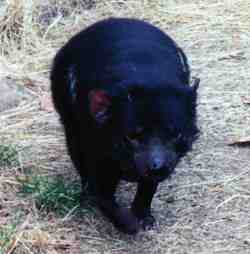
\includegraphics[width=\marginparwidth]{Matrices/tasmanianDevil}
Tasmanian Devil}
two-thirds of the female newborns survive to be one year old;
two-thirds of female one year olds survive to be two years old;
one-half of female two year olds survive to be three years old;
each year, each female aged two or three years gives birth to two female offspring;
female Tasmanian Devils survive for four years, at most.

Analogous to \autoref{eg:matasp} define a vector \(\xv\) in~\(\RR^4\) to be the number of females of specified ages.
Use the above information to write down the \idx{Leslie matrix}~\(L\) that predicts the number in the next year,~\(\xv'\), from the number in any year,~\xv.
Given the observed initial female numbers of \(18\)~newborns, \(9\)~one year olds, \(18\)~two year olds, and \(18\)~three year olds, use matrix multiplication to predict the numbers of female Tasmanian Devils one, two and three years later.
Does the population appear to be increasing? or decreasing?
\answer{Let \(x_j\) be the number of females of age \((j-1)\)~years.
\(L=\protect\begin{bmat} 0&0&2&2\protect\\ 2/3&0&0&0\protect\\ 0&2/3&0&0\protect\\ 0&0&1/2&0 \protect\end{bmat}\).
After one year \(\xv'=(72,12,6,9)\), two years \(\xv''=(30,48,8,3)\), three years \(\xv'''=(22,20,32,4)\).
Increasing.}
\end{exercise}


\begin{comment}
Many Markov Chain possibilities, especially age structured populations, maybe snakes and ladders, and compute powers.
\end{comment}







\begin{exercise}  
Write down the \idx{transpose} of each of the following matrices.
Which of the following matrices are a \idx{symmetric matrix}?
\begin{Parts}
\item \(\begin{bmatrix} -2&3
\\3&0
\\-8&2
\\-2&-4 \end{bmatrix}\)
\answer{\(\protect\begin{bmat} -2&3&-8&-2
\protect\\3&-0&2&-4 \protect\end{bmat}\)}

\item \(\begin{bmatrix} 3&-4&-2&2
\\-5&2&-3&3 \end{bmatrix}\)
\answer{\(\protect\begin{bmat} 3&-5
\protect\\-4&2
\protect\\-2&-3
\protect\\2&3 \protect\end{bmat}\)}

\item \(\begin{bmatrix} 14&5&3&2 
\\5&0&-1&1 
\\3&-1&-6&-4
\\2&1&-4&4 \end{bmatrix}\)
\answer{\(\protect\begin{bmat} 14&5&3&2 
\protect\\5&0&-1&1 
\protect\\3&-1&-6&-4
\protect\\2&1&-4&4&\protect\end{bmat}\), symmetric}

\begin{reduce}
\item \(\begin{bmatrix} 3&1&-2&-3 \end{bmatrix}\)
\answer{\(\protect\begin{bmat} 3
\protect\\1
\protect\\-2
\protect\\-3 \protect\end{bmat}\)}

\item \(\begin{bmatrix} 5&-1&-2&2
\\1&-2&-2&0
\\-1&-5&4&-1
\\5&2&-1&-2 \end{bmatrix}\)
\answer{\(\protect\begin{bmat} 5&1&-1&5
\protect\\-1&-2&-5&2
\protect\\-2&-2&4&-1
\protect\\2&0&-1&-2 \protect\end{bmat}\)}
\end{reduce}

\item \(\begin{bmatrix} -4&-5.1&0.3
\\-5.1&-7.4&-3.
\\0.3&-3&2.6 \end{bmatrix}\)
\answer{\(\protect\begin{bmat} -4&-5.1&0.3
\protect\\-5.1&-7.4&-3
\protect\\0.3&-3.&2.6 \protect\end{bmat}\), symmetric}

\item \(\begin{bmatrix} -1.5&-0.6&-1.7
\\-1&-0.4&-5.6 \end{bmatrix}\)
\answer{\(\protect\begin{bmat} -1.5&-1
\protect\\-0.6&-0.4
\protect\\-1.7&-5.6 \protect\end{bmat}\)}

\item \(\begin{bmatrix} 1.7&-0.2&-0.4
\\0.7&-0.3&-0.4
\\0.6&3&-2.2 \end{bmatrix}\)
\answer{\(\protect\begin{bmat} 1.7&0.7&0.6
\protect\\-0.2&-0.3&3
\protect\\-0.4&-0.4&-2.2 \protect\end{bmat}\)}
\end{Parts}
%m=ceil(4*rand),n=ceil(4*rand),a=round(randn(m,n)*20)/10+0,a'
\end{exercise}

\begin{exercise}  
For each of the following matrices, are they symmetric? 
\(I_4\), \(I_{3\times4}\), \(O_3\), and~\(O_{3\times1}\).
\answer{yes, no, yes, no.}
\end{exercise}




\begin{exercise}  
Use \script\ to generate some random matrices of a suitable \idx{size} of your choice, and some random scalars (see \autoref{tbl:mtlbops}).
Choose some suitable exponents.
Recalling that in \script\ the dash~\verb|'| performs the transpose, confirm the matrix \idx{transpose} properties of \autoref{thm:pot}.
Record all your commands and the output from \script.
\end{exercise}


\begin{exercise}  
Use \autoref{def:mattran} of the matrix \idx{transpose} to prove \cref{thm:pota,thm:potc}.
\end{exercise}

\begin{exercise}  
Use the other parts of \autoref{thm:pot} to prove parts~\ref{thm:pote} and~\ref{thm:potf}.
\end{exercise}


\begin{exercise}  
In a few sentences, answer\slash discuss each of the following.
\begin{enumerate}
\item Why is the size of a matrix important?

\item What causes these identities to hold? \(A\pm O=A\) and \(A-A=O\).

\item In the matrix product~\(AB\), why do the number of columns of~\(A\) have to be the same as the number of rows of~\(B\)?

\item What can you say about the sizes of matrices~\(A\) and~\(B\) if both products~\(AB\) and~\(BA\) are computable?

\item What causes multiplication of a vector by a square matrix to be viewed as a transformation?

\item What causes the identity matrix to be zero except for ones along the diagonal from the top-left to the bottom-right?

\item How does multiplication by a square matrix arise in studying the age structure of populations?

\item Why is it impossible to compute powers of a non-square matrix?

\item Why did we invoke random matrices?

\item Among all the properties for matrix addition and multiplication operations, which ones are different to the analogous properties for scalars?  why?

\item What constraint must be put on matrix~\(A\) in order for \(A+\tr A\) to be defined?  
What constraint must be put on matrix~\(B\) in order for \(B\tr B\) to be defined?  
Give reasons.

\end{enumerate}
\end{exercise}



\begin{comment}%{ED498555.pdf}
why, what caused X?
how did X occur?
what-if? what-if-not?
how does X compare with Y?
what is the evidence for X?
why is X important?
\end{comment}





%!TEX root = ../larxxia.tex

\section{The inverse of a matrix}
\label{sec:im}

\secttoc

\begin{comment}
\pooliv{p.163--9}  \layiv{\S2.2--3}  \cite[\S3.2]{Nakos1998}  \cite[Ch.~6]{Chartier2015}
\end{comment}


The previous \autoref{sec:moaa} introduced addition, subtraction, multiplication, and other operations of matrices.  
Conspicuously missing from the list is `division' by a matrix.
This section develops `division' by a matrix as multiplication by the inverse of a matrix.
The analogue in ordinary arithmetic is that division by ten is the same as multiplying by its reciprocal, one-tenth.
But the inverse of a matrix looks nothing like a reciprocal.


\subsection{Introducing the unique inverse}

Let's start with an example that illustrates an analogy with the reciprocal\slash inverse of a scalar number.

\begin{example} \label{eg:a2x2inv}
%while abs(det(A))~=1, A=round(randn(2,2)*5), end, B=inv(A)
Recall that a crucial property is that a number multiplied by its reciprocal\slash inverse is one: for example, \(2\times 0.5=1\) so \(0.5\) is the reciprocal\slash inverse of~\(2\).
Similarly, show that matrix 
\begin{equation*}
B=\begin{bmatrix} -3&1\\-4&1 \end{bmatrix}
\text{ is an inverse of }
A=\begin{bmatrix} 1&-1\\4&-3 \end{bmatrix}
\end{equation*}
by showing their product is the \(2\times2\) \idx{identity matrix}~\(I_2\).
\begin{solution} 
Multiply 
\begin{equation*}
AB=\begin{bmatrix} 1&-1\\4&-3 \end{bmatrix}
\begin{bmatrix} -3&1\\-4&1 \end{bmatrix}
=\begin{bmatrix} 1&0\\0&1 \end{bmatrix}=I_2
\end{equation*}
the multiplicative identity.  
But matrix multiplication is not commutative (\autoref{sec:fapmo}), so also consider
\begin{equation*}
BA=\begin{bmatrix} -3&1\\-4&1 \end{bmatrix}
\begin{bmatrix} 1&-1\\4&-3 \end{bmatrix}
=\begin{bmatrix} 1&0\\0&1 \end{bmatrix}=I_2\,.
\end{equation*}
That these products are the identity---analogous to the number one in scalar arithmetic---means that the matrix~\(A\) has the same relation to the matrix~\(B\) as a number has to its reciprocal\slash inverse.
\marginpar{\begin{tikzpicture}[]
\begin{axis}[footnotesize,font=\footnotesize%,width=12em
    , axis equal , axis lines=middle,
    , grid, xmax=4.5,ymax=5.5 ]
    \addplot[blue,quiver={u=2,v=1},-stealth, thick] coordinates {(0,0)};
    \node[right] at (axis cs:2,1) {$(2,1)$};
    \addplot[red,quiver={u=1,v=5},-stealth, thick] coordinates {(0,0)};
    \node[right] at (axis cs:1,5) {$A(2,1)$};
\end{axis}
\end{tikzpicture}}%

Being the inverse, matrix~\(B\) `undoes' the action of matrix~\(A\)---as illustrated in the margin.
The first picture shows multiplication by~\(A\) transforms the vector~\((2,1)\) to the vector~\((1,5)\): \(A\footnotesize\begin{bmatrix} 2\\1 \end{bmatrix}=\begin{bmatrix} 1\\5 \end{bmatrix}\).
The second picture shows that multiplication by~\(B\) undoes the transform by~\(A\) because \(B\footnotesize\begin{bmatrix} 1\\5 \end{bmatrix}=\begin{bmatrix} 2\\1 \end{bmatrix}\) the original vector.
\marginpar{%
\begin{tikzpicture}[]
\begin{axis}[footnotesize,font=\footnotesize%,width=12em
    , axis equal, axis lines=middle,
    , grid, xmax=4.5,ymax=5.5 ]
    \addplot[red,quiver={u=2,v=1},-stealth, thick] coordinates {(0,0)};
    \node[right] at (axis cs:2,1) {$B(1,5)$};
    \addplot[blue,quiver={u=1,v=5},-stealth, thick] coordinates {(0,0)};
    \node[right] at (axis cs:1,5) {$(1,5)$};
\end{axis}
\end{tikzpicture}
}%
\end{solution}
\end{example}

The previous \autoref{eg:a2x2inv} shows at least one case when we can do some sort of matrix `division': that is, multiplying by~\(B\) is equivalent to `dividing' by~\(A\).
One restriction is that a clearly defined `division' only works for square matrices because we need to be able to compute both~\(AB\) and~\(BA\).


\begin{definition}[inverse] \label{def:invertible} 
For every \(n\times n\) \idx{square matrix}~\(A\), an \bfidx{inverse} of~\(A\) is an \(n\times n\) matrix~\(B\) such that both \(AB=I_n\) and \(BA=I_n\)\,.
If such a matrix~\(B\) exists, then matrix~\(A\) is called \bfidx{invertible}.
\end{definition}

\begin{example} \label{eg:a3x3inv}
%A=round(randn(3,3)*5),B=inv(A)
Show that matrix
\begin{equation*}
B=\begin{bmatrix} 0&-\frac14&-\frac18\\\frac32&1&\frac78\\ \frac12&\frac14&\frac38 \end{bmatrix}
\text{ is an inverse of }
A=\begin{bmatrix} 1&-1&5\\-5&-1&3\\2&2&-6 \end{bmatrix}.
\end{equation*}

\begin{solution} 
First compute 
\begin{align*}
&AB=\begin{bmatrix} 1&-1&5\\-5&-1&3\\2&2&-6 \end{bmatrix}
\begin{bmatrix} 0&-\frac14&-\frac18\\\frac32&1&\frac78\\ \frac12&\frac14&\frac38 \end{bmatrix}
\\&=\footnotesize\let\cdt\cdot\def\cdot{\!\cdt\!}%squeeze it
\begin{bmatrix} 
1\cdot0 -1\cdot\frac32 +5\cdot\frac12&
1\cdot(-\frac14) -1\cdot1 +5\cdot\frac14&
1\cdot(-\frac18) -1\cdot\frac78 +5\cdot\frac38\\
-5\cdot0 -1\cdot\frac32 +3\cdot\frac12&
-5\cdot(-\frac14) -1\cdot1 +3\cdot\frac14&
-5\cdot(-\frac18) -1\cdot\frac78 +3\cdot\frac38\\
2\cdot0 +2\cdot\frac32 -6\cdot\frac12&
2\cdot(-\frac14) +2\cdot1 -6\cdot\frac14&
2\cdot(-\frac18) +2\cdot\frac78 -6\cdot\frac38
\end{bmatrix}
\\&=\begin{bmatrix} 1&0&0\\ 0&1&0\\ 0&0&1 \end{bmatrix}=I_3\,.
\end{align*}
Second compute
\begin{align*}
&BA=
\begin{bmatrix} 0&-\frac14&-\frac18\\\frac32&1&\frac78\\ \frac12&\frac14&\frac38 \end{bmatrix}
\begin{bmatrix} 1&-1&5\\-5&-1&3\\2&2&-6 \end{bmatrix}
\\&=\footnotesize\let\cdt\cdot\def\cdot{\!\cdt\!}%squeeze it
\begin{bmatrix}  
      0\cdot1 -\frac14\cdot(-5) -\frac18\cdot2 &
      0\cdot(-1) -\frac14\cdot(-1) -\frac18\cdot2 &
      0\cdot5 -\frac14\cdot3 -\frac18\cdot(-6) \\
\frac32\cdot1 +1\cdot(-5) +\frac78\cdot2 &
\frac32\cdot(-1) +1\cdot(-1) +\frac78\cdot2 &
\frac32\cdot5 +1\cdot3 +\frac78\cdot(-6) \\
\frac12\cdot1 +\frac14\cdot(-5) +\frac38\cdot2 &
\frac12\cdot(-1) +\frac14\cdot(-1) +\frac38\cdot2 &
\frac12\cdot5 +\frac14\cdot3 +\frac38\cdot(-6) 
\end{bmatrix}
\\&=\begin{bmatrix} 1&0&0\\ 0&1&0\\ 0&0&1 \end{bmatrix}=I_3\,.
\end{align*}
Since both of these products are the identity, then matrix~\(A\) is invertible, and \(B\)~is an inverse of~\(A\).
\end{solution}
\end{example}




\begin{activity}
What value of~\(b\) makes matrix \(\begin{bmatrix} -1&b\\1&2 \end{bmatrix}\) the inverse of
\(\begin{bmatrix} 2&3\\-1&-1 \end{bmatrix}\)?
% a=0+round(randn(2)*3),b=inv(a)
\actposs[4]{\(-3\)}{\(-2\)}{\(1\)}{\(3\)}
%\partswidth=5em
%\begin{parts}
%\item \(-3\)\actans
%\item \(-2\)
%\item \(1\)
%\item \(3\)
%\end{parts}
\end{activity}





But even among square matrices, there are many non-zero matrices which do not have inverses!
The next \autoref{sec:fisvd} further explores why some matrices do not have an inverse: the reason is associated with both \index{rcond()@\texttt{rcond()}}\verb|rcond| being zero (\autoref{pro:unisol}) and/or the so-called determinant being zero (\autoref{ch:ddm}).

\begin{example}[no inverse] \label{eg:no2x2inv}
Prove that the matrix
\begin{equation*}
A=\begin{bmatrix} 1&-2\\-3&6 \end{bmatrix}
\end{equation*}
does not have an inverse.
\begin{solution} 
Assume there is an inverse matrix
\begin{equation*}
B=\begin{bmatrix} a&b\\c&d \end{bmatrix}.
\end{equation*}
Then by \autoref{def:invertible} the product \(AB=I_2\); that is,
\begin{eqnarray*}
AB&=&\begin{bmatrix} 1&-2\\-3&6 \end{bmatrix}
\begin{bmatrix} a&b\\c&d \end{bmatrix}
\\&=&\begin{bmatrix} a-2c&b-2d\\-3a+6c&-3b+6d \end{bmatrix}
=\begin{bmatrix} 1&0\\0&1 \end{bmatrix}.
\end{eqnarray*}
The bottom-left entry in this matrix equality asserts \(-3a+6c=0\) which is \(-3(a-2c)=0\), that is, \(a-2c=0\)\,.
But the top-left entry in the matrix equality asserts \(a-2c=1\)\,.
Both of these equations involving~\(a\) and~\(c\) cannot be true simultaneously; therefore the assumption of an inverse must be incorrect.
The matrix~\(A\) does not have an inverse.
\end{solution}
\end{example}



\begin{theorem}[unique inverse] \label{thm:uninv} 
If \(A\) is an \idx{invertible} matrix, then its \idx{inverse} is unique (and denoted by~\(A^{-1}\)).
\end{theorem}
\begin{proof} 
We suppose there are two inverses, say \(B_1\) and~\(B_2\), and proceed to show they must be the same.
Since they are inverses, by \autoref{def:invertible} both
\(AB_1=B_1A=I_n\) and \(AB_2=B_2A=I_n\)\,.
Consequently, using associativity of matrix multiplication (\autoref{thm:pmma}),
\begin{equation*}
B_1=B_1I_n=B_1(AB_2)=(B_1A)B_2=I_nB_2=B_2\,.
\end{equation*}
That is, \(B_1=B_2\) and so the inverse is unique.
\end{proof}



In the elementary case of \(1\times1\) matrices, that is \(A=\begin{bmatrix} a_{11} \end{bmatrix}\), the inverse is simply the reciprocal of the entry, that is \(A^{-1}=\begin{bmatrix} 1/a_{11} \end{bmatrix}\) provided \(a_{11}\)~is non-zero.
The reason is that \(AA^{-1}=\begin{bmatrix} a_{11}\cdot\frac1{a_{11}} \end{bmatrix}=\begin{bmatrix} 1 \end{bmatrix}=I_1\) and  \(A^{-1}A=\begin{bmatrix} \frac1{a_{11}}\cdot a_{11} \end{bmatrix}=\begin{bmatrix} 1 \end{bmatrix}=I_1\)\,.

In the case of \(2\times2\) matrices the inverse is a little more complicated, but should be remembered.

\begin{theorem}[\(2\times2\) inverse] \label{thm:2x2det} 
Let \(2\times2\) matrix \(A=\begin{bmatrix} a&b\\c&d \end{bmatrix}\). Then \(A\)~is \idx{invertible} if the \bfidx{determinant} \(ad-bc\neq0\)\,, in which case
\begin{equation}
A^{-1}=\frac1{ad-bc}\begin{bmatrix} d&-b\\-c&a \end{bmatrix}.
\label{eq:2x2inv}
\end{equation}
If the determinant \(ad-bc=0\)\,, then \(A\)~is not \idx{invertible}.
\end{theorem}

\begin{example} \label{eg:}
\begin{enumerate}
\item Recall \autoref{eg:a2x2inv} verified that
\begin{equation*}
B=\begin{bmatrix} -3&1\\-4&1 \end{bmatrix}
\text{ is an inverse of }
A=\begin{bmatrix} 1&-1\\4&-3 \end{bmatrix}.
\end{equation*}
Formula~\eqref{eq:2x2inv} gives this inverse from the matrix~\(A\): its elements are \(a=1\)\,, \(b=-1\)\,, \(c=4\) and \(d=-3\) so the determinant \(ad-bc=1\cdot(-3)-(-1)\cdot4=1\) and hence formula~\eqref{eq:2x2inv} derives the inverse
\begin{equation*}
A^{-1}=\frac11\begin{bmatrix} -3&-(-1)\\-4&1 \end{bmatrix}
=\begin{bmatrix} -3&1\\-4&1 \end{bmatrix}=B\,.
\end{equation*}

\item Further, recall \autoref{eg:no2x2inv} proved there is no inverse for matrix
\begin{equation*}
A=\begin{bmatrix} 1&-2\\-3&6 \end{bmatrix}.
\end{equation*}
\autoref{thm:2x2det} also establishes this matrix is not invertible because the matrix determinant \(ad-bc=1\cdot6-(-2)\cdot(-3)=6-6=0\)\,. 
\end{enumerate}
\end{example}




\begin{activity}
Which of the following matrices is invertible?
\actposs{\(\begin{bmatrix} 0&-3\\4&-2 \end{bmatrix}\)}
{\(\begin{bmatrix} -2&-1&4\\3&1&1 \end{bmatrix}\)}
{\(\begin{bmatrix} -2&1\\4&-2 \end{bmatrix}\)}
{\(\begin{bmatrix} -4&-2\\2&2\\-3&1 \end{bmatrix}\)}
%\begin{parts}
%\item \(\begin{bmatrix} -2&-1&4\\3&1&1 \end{bmatrix}\)
%\item \(\begin{bmatrix} 0&-3\\4&-2 \end{bmatrix}\)\actans
%\item \(\begin{bmatrix} -2&1\\4&-2 \end{bmatrix}\)
%\item \(\begin{bmatrix} -4&-2\\2&2\\-3&1 \end{bmatrix}\)
%\end{parts}
\end{activity}



\begin{proof} 
To prove \autoref{thm:2x2det}, first show the given~\(A^{-1}\) satisfies \autoref{def:invertible} when the determinant \(ad-bc\neq 0\) (and using associativity of scalar-matrix multiplication, \autoref{thm:pmmc}).
For the proposed~\(A^{-1}\), on the one hand,
\begin{eqnarray*}
A^{-1}A&=&\frac1{ad-bc}\begin{bmatrix} d&-b\\-c&a \end{bmatrix}
\begin{bmatrix} a&b\\c&d \end{bmatrix}
\\&=&\frac1{ad-bc}\begin{bmatrix} da-bc&db-bd\\-ca+ac&-cb+ad \end{bmatrix}
\\&=&\begin{bmatrix} 1&0\\0&1 \end{bmatrix}=I_2\,.
\end{eqnarray*}
On the other hand,
\begin{eqnarray*}
AA^{-1}&=&
\begin{bmatrix} a&b\\c&d \end{bmatrix}\begin{bmatrix} d&-b\\-c&a \end{bmatrix}\frac1{ad-bc}
\\&=&\begin{bmatrix} ad-bc&-ab+ba\\cd-dc&-cb+da \end{bmatrix}\frac1{ad-bc}
\\&=&\begin{bmatrix} 1&0\\0&1 \end{bmatrix}=I_2\,.
\end{eqnarray*}
By uniqueness (\autoref{thm:uninv}), equation~\eqref{eq:2x2inv} is the only inverse when \(ad-bc\neq 0\)\,.

Now eliminate the case when \(ad-bc=0\)\,.
If an inverse exists, say~\(X\), then it must satisfy \(AX=I_2\).
The top-left entry of this matrix equality requires \(ax_{11}+bx_{21}=1\)\,, whereas the bottom-left equality requires \(cx_{11}+dx_{21}=0\)\,.
Regard these as a system of two linear equations for the as yet unknowns \(x_{11}\) and~\(x_{21}\): from \(d\times\)~the first subtract \(b\times\)~the second to deduce that an inverse requires
\(dax_{11}+dbx_{21}-bcx_{11}-bdx_{21}=d\cdot1-b\cdot0\)\,.
By cancellation and factorising~\(x_{11}\), this equation then requires \((ad-bc)x_{11}=d\)\,.
But the determinant is zero, so this equation requires \(0\cdot x_{11}=d\)\,.
\begin{itemize}
\item If element~\(d\) is non-zero, then this equation cannot be satisfied and hence no inverse can be found.
\item Otherwise, if \(d\) is zero, then any~\(x_{11}\) satisfies this equation so if there is an inverse then there would be an infinite number of inverses (through the free variable~\(x_{11}\)).
But this contradicts the uniqueness \autoref{thm:uninv} so an inverse cannot exist in this case either.
\end{itemize}
That is, if the determinant \(ad-bc=0\)\,, then the \(2\times2\) matrix is not invertible.
\end{proof}



\begin{quoted}{\parbox[t]{0.5\linewidth}{G.~E. Forsythe and C.~B. Moler, 1967 \cite[p.261]{Higham1996}}}
Almost anything you can do with \(A^{-1}\) can be done without it.
\end{quoted}


\paragraph{Computer considerations} 
Except for easy cases such as \(2\times2\) matrices, we rarely explicitly compute the \idx{inverse} of a matrix.
Computationally there are (almost) always better ways such as the \script\ operation~\verb|A\b| of \autoref{pro:unisol}.
The \idx{inverse} is a crucial theoretical device, rarely a practical computational tool.


The following \autoref{thm:invuniqsol} is an example: for a system of linear equations the theorem connects the existence of a unique solution to the invertibility of the matrix of coefficients.
Further, \autoref{sec:svdsgs} connects solutions to the \verb|rcond| invoked by \autoref{pro:unisol}.
Although in theoretical statements we write expressions like \(\xv=A^{-1}\bv\)\,,
practically, once we know a solution exists (\verb|rcond| is acceptable), we generally compute the solution without ever constructing~\(A^{-1}\).



\begin{theorem} \label{thm:invuniqsol} 
If \(A\) is an \idx{invertible} \(n\times n\) matrix, then the system of \idx{linear equation}s \(A\xv=\bv\) has the \idx{unique solution} \(\xv=A^{-1}\bv\) for every \(\bv\) in~\(\RR^n\).
\end{theorem}

One consequence is the following: if a system of linear equations has no solution or an infinite number of solutions (\autoref{thm:fred}), then this theorem establishes that the matrix of the system is not invertible.

\begin{proof} 
The proof has two parts: first showing \(\xv=A^{-1}\bv\) is a solution, and second showing that there are no others.
First,  try \(\xv=A^{-1}\bv\) and use associativity (\autoref{thm:pmma}) and the inverse \autoref{def:invertible}:
\begin{equation*}
A\xv=A(A^{-1}\bv)=(AA^{-1})\bv=I_n\bv=\bv\,.
\end{equation*}
Second, suppose~\yv\ is any solution, that is, \(A\yv=\bv\)\,.
Multiply both sides by the inverse~\(A^{-1}\), and again use associativity and the definition of the inverse, to deduce
\begin{eqnarray*}
A^{-1}(A\yv)=A^{-1}\bv
&\implies& (A^{-1}A)\yv=\xv
\\&\implies& I_n\yv=\xv
\\&\implies& \yv=\xv\,.
\end{eqnarray*}
Since any solution~\yv\ has to be the same as~\xv, \(\xv=A^{-1}\bv\) is the unique solution.
\end{proof}





\begin{example} \label{eg:}
Use the matrices of Examples~\ref{eg:a2x2inv}, \ref{eg:a3x3inv} and~\ref{eg:no2x2inv} to decide whether the following systems have a unique solution, or not.
\begin{parts}
\item \(\begin{cases}
x-y=4\,,\\4x-3y=3\,.
\end{cases}\)
\item \(\begin{cases}
u-v+5w=2\,,\\ -5u-v+3w=5\,,\\ 2u+2v-6w=1\,.
\end{cases}\)
\item \(\begin{cases}
r-2s=-1\,,\\-3r+6s=3\,.
\end{cases}\)
\end{parts}
\begin{solution} 
\begin{enumerate}
\item A matrix for this system is \(\footnotesize\begin{bmatrix} 1&-1\\4&-3 \end{bmatrix}\) which \autoref{eg:a2x2inv} shows has an inverse.  
\autoref{thm:invuniqsol} then assures us the system has a unique solution.
\item A matrix for this system is \(\footnotesize\begin{bmatrix} 1&-1&5\\-5&-1&3\\2&2&-6 \end{bmatrix}\) which \autoref{eg:a3x3inv} shows has an inverse.  
\autoref{thm:invuniqsol} then assures us the system has a unique solution.
\item A matrix for this system is \(\footnotesize\begin{bmatrix} 1&-2\\-3&6 \end{bmatrix}\) which \autoref{eg:no2x2inv} shows is not invertible.  
\autoref{thm:invuniqsol} then assures us the system does not have a unique solution.
By \autoref{thm:fred} there may be either no solution or an infinite number of solutions---the matrix alone does not tell us which.
\end{enumerate}
\end{solution}
\end{example}






\begin{example} \label{eg:}
Given the following information about solutions of systems of linear equations, write down if the matrix associated with each system is invertible, or not, or there is not enough given information to decide.  Give reasons.
\begin{parts}
\item A general solution is \((1,-5,0,3)\).
\item A general solution is \((3,-5+3t,3-t,-1)\).
\item A solution of a system is \((-3/2,-2,-\pi,2,-4)\).
\item A solution of a homogeneous system is \((1,2,-8)\).
\end{parts}
\begin{solution} 
\begin{enumerate}
\item Since the solution is unique, the matrix in the system must be invertible.
\item This solution has an apparent free parameter,~\(t\), and so there are many solutions which implies the matrix is not invertible.
\item Not enough information is given as we do not know whether there are any more solutions.
\item Since a homogeneous system always has~\ov\ as a solution (\autoref{sec:3pns}), then we know that there are at least two solutions to the system, and hence the matrix is not invertible.
\end{enumerate}
\end{solution}
\end{example}




Recall from \autoref{sec:moaa} the properties of scalar multiplication, matrix powers, transpose, and their computation (\autoref{tbl:mtlbops}).
The next theorem incorporates the inverse into this suite of properties.


\begin{theorem}[properties of the inverse] \label{thm:invprop} 
Let \(A\) and~\(B\) be \idx{invertible} matrices of the same size, then:
\begin{enumerate}
\item\label{thm:invpropa}  matrix \(A^{-1}\) is invertible and \((A^{-1})^{-1}=A\)\,;
\item\label{thm:invpropb} if scalar \(c\neq0\)\,, then matrix~\(cA\) is invertible and \((cA)^{-1}=\frac1cA^{-1}\);
\item\label{thm:invpropc}\begin{aside}
The reversed order is important in the identity $(AB)^{-1}=B^{-1}A^{-1}$.
\end{aside} 
matrix \(AB\) is invertible and \((AB)^{-1}=B^{-1}A^{-1}\);
\item\label{thm:invpropd} matrix \(\tr A\) is invertible and \((\tr A)^{-1}=\tr{(A^{-1})}\);
\item\label{thm:invprope} matrices \(A^p\) are invertible for all \(p=1,2,3,\ldots\) and \((A^p)^{-1}=(A^{-1})^p\).
\end{enumerate}
\end{theorem}


\begin{proof} 
Three parts are proved, and two are left as exercises.
\begin{description}
\item[\ref{thm:invpropa}]
By \autoref{def:invertible} the matrix~\(A^{-1}\) satisfies \(A^{-1}A=AA^{-1}=I\)\,.
But also by \autoref{def:invertible} this is exactly the identities we need to assert that matrix~\(A\) is the inverse of matrix~\((A^{-1})\).
Hence \(A=(A^{-1})^{-1}\).

\item[\ref{thm:invpropc}]
Test that \(B^{-1}A^{-1}\) has the required properties for the inverse of~\(AB\).
First, by associativity (\autoref{thm:pmma}) and multiplication by the identity (\autoref{thm:pmmd})
\begin{equation*}
(B^{-1}A^{-1})(AB)
=B^{-1}(A^{-1}A)B
=B^{-1}IB
=B^{-1}B
=I\,.
\end{equation*}
Second, and similarly
\begin{equation*}
(AB)(B^{-1}A^{-1})
=A(BB^{-1})A^{-1}
=AIA^{-1}
=AA^{-1}
=I\,.
\end{equation*}
Hence by \autoref{def:invertible} and the uniqueness \autoref{thm:uninv}, matrix~\(AB\) is invertible and \(B^{-1}A^{-1}\) is the inverse.

\item[\ref{thm:invprope}]
Prove by induction and use~\ref{thm:invpropc}.
\begin{itemize}
\item For the case of exponent \(p=1\)\,, \((A^1)^{-1}=(A)^{-1}=A^{-1}=(A^{-1})^1\) and so the identity holds.
\item For any integer exponent \(p\geq2\)\,, assume the identity \((A^{p-1})^{-1}=(A^{-1})^{p-1}\).
Consider 
\begin{eqnarray*}
(A^p)^{-1}&=&(AA^{p-1})^{-1}\quad(\text{by power law Thm.~\ref{thm:pmmg}})
\\&=&(A^{p-1})^{-1}A^{-1}\quad(\text{by Thm.~\ref{thm:invpropc}, }B=A^{p-1})
\\&=&(A^{-1})^{p-1}A^{-1}\quad(\text{by inductive assumption})
\\&=&(A^{-1})^p \quad(\text{by power law Thm.~\ref{thm:pmmg}}).
\end{eqnarray*}
\item By induction, the identity \((A^{p})^{-1}=(A^{-1})^{p}\) holds for exponents \(p=1,2,3,\ldots\)\,.
\end{itemize}
 
\end{description}
\end{proof}




\begin{activity}
The matrix \(\begin{bmatrix} 3&-5\\4&-7 \end{bmatrix}\) has inverse \(\begin{bmatrix} 7&-5\\4&-3 \end{bmatrix}\).
\begin{itemize}
\item What is the inverse of the matrix \(\begin{bmatrix} 6&-10\\8&-14 \end{bmatrix}\)?
% for i=1:999, a=0+round(randn(2)*4); if abs(det(a))==1, a=a, break,end, end
\actposs{\(\begin{bmatrix} 3.5&-2.5\\2&-1.5 \end{bmatrix}\)}
{\(\begin{bmatrix} 14&-10\\8&-3 \end{bmatrix}\)}
{\(\begin{bmatrix} 3.5&2\\-2.5&-1.5 \end{bmatrix}\)}
{\(\begin{bmatrix} 7&4\\-5&-3 \end{bmatrix}\)}
%\begin{parts}
%\item \(\begin{bmatrix} 14&-10\\8&-3 \end{bmatrix}\)
%\item \(\begin{bmatrix} 3.5&-2.5\\2&-1.5 \end{bmatrix}\)
%\item \(\begin{bmatrix} 3.5&2\\-2.5&-1.5 \end{bmatrix}\)
%\item \(\begin{bmatrix} 7&4\\-5&-3 \end{bmatrix}\)
%\end{parts}
\item Further, which of the above is the inverse of \(\begin{bmatrix} 3&4\\-5&-7 \end{bmatrix}\)?
\end{itemize}
\end{activity}





\begin{definition}[non-positive powers] \label{def:invpow} 
For every \idx{invertible} matrix~\(A\), define \(A^0:=I\) and for every positive integer~\(p\) define \(A^{-p}:=(A^{-1})^p\) (or by \autoref{thm:invprope} equivalently as~\((A^p)^{-1}\)).
\end{definition}

\begin{example} \label{eg:a2x2negp}
Recall from \autoref{eg:a2x2inv} that matrix
\begin{equation*}
A=\begin{bmatrix} 1&-1\\4&-3 \end{bmatrix}
\text{ has inverse }
A^{-1}=\begin{bmatrix} -3&1\\-4&1 \end{bmatrix}.
\end{equation*}
Compute \(A^{-2}\) and~\(A^{-4}\).
\begin{solution} 
From \autoref{def:invpow},
\begin{eqnarray*}
A^{-2}&=&(A^{-1})^2
=\begin{bmatrix} -3&1\\-4&1 \end{bmatrix}\begin{bmatrix} -3&1\\-4&1 \end{bmatrix}
=\begin{bmatrix} 5&-2\\8&-3 \end{bmatrix},
\\
A^{-4}&=&(A^{-1})^4
=\big[(A^{-1})^2\big]^2
\\&=&\begin{bmatrix} 5&-2\\8&-3 \end{bmatrix}\begin{bmatrix} 5&-2\\8&-3 \end{bmatrix}
=\begin{bmatrix} 9&-4\\16&-7 \end{bmatrix},
\end{eqnarray*}
upon using one of the power laws of \autoref{thm:pmmg}.
\end{solution}
\end{example}



\begin{activity}
\autoref{eg:a2x2negp} gives the inverse of a matrix~\(A\) and determines~\(A^{-2}\): what is~\(A^{-3}\)?
\actposs{\(\begin{bmatrix} -7&3\\-12&5 \end{bmatrix}\)}
{\(\begin{bmatrix} 3&-7\\5&-12 \end{bmatrix}\)}
{\(\begin{bmatrix} -7&-12\\3&5 \end{bmatrix}\)}
{\(\begin{bmatrix} 3&5\\-7&-12 \end{bmatrix}\)}
%\begin{parts}
%\item \(\begin{bmatrix} -7&3\\-12&5 \end{bmatrix}\)\actans
%\item \(\begin{bmatrix} 3&-7\\5&-12 \end{bmatrix}\)
%\item \(\begin{bmatrix} -7&-12\\3&5 \end{bmatrix}\)
%\item \(\begin{bmatrix} 3&5\\-7&-12 \end{bmatrix}\)
%\end{parts}
\end{activity}




\begin{example}[predict the past] \label{eg:invph}
Recall \autoref{eg:matasp} introduced how to use a \idx{Leslie matrix} to predict the future population of an animal.
If \(\xv=(60,70,20)\) is the current number of pups, juveniles, and mature females respectively, then, for the Leslie matrix
\begin{equation*}
L=\begin{bmatrix} 0&0&4\\\frac12&0&0\\0&\frac13&\frac13 \end{bmatrix},
\quad\text{which has inverse }L^{-1}=\begin{bmatrix} 0&2&0\\-\frac14&0&3\\\frac14&0&0 \end{bmatrix},
\end{equation*} 
 by the modelling the predicted population numbers after a year is \(\xv'=L\xv\), after two years is \(\xv''=L\xv'=L^2\xv\), and so on.
Assume the same rule applies for earlier years.
\begin{itemize}
\item Letting the population numbers a year ago be denoted by~\(\xv^-\) then by the modelling the current population \(\xv=L\xv^-\).
Multiply by the inverse of~\(L\): \(L^{-1}\xv=L^{-1}L\xv^-=\xv^-\); that is, the population a year before the current is \(\xv^-=L^{-1}\xv\).
\item Similarly, letting the population numbers two years ago be denoted by~\(\xv^=\) then  by the modelling \(\xv^-=L\xv^=\) and multiplication by~\(L^{-1}\) gives \(\xv^==L^{-1}\xv^-=L^{-1}L^{-1}\xv=L^{-2}\xv\).
\item One more year earlier, letting the population numbers two years ago be denoted by~\(\xv^\equiv\) then  by the modelling \(\xv^==L\xv^\equiv\) and multiplication by~\(L^{-1}\) gives \(\xv^\equiv=L^{-1}\xv^==L^{-1}L^{-2}\xv=L^{-3}\xv\).
\end{itemize}
Hence use the inverse powers of~\(L\) to predict the earlier history of the population of female animals in the given example: but first verify the given inverse is correct.
\begin{solution} 
Verify the given inverse by evaluating (showing only non-zero terms in a sum)
\begin{eqnarray*}
LL^{-1}&=&
\begin{bmatrix} 0&0&4\\\frac12&0&0\\0&\frac13&\frac13 \end{bmatrix}
\begin{bmatrix} 0&2&0\\-\frac14&0&3\\\frac14&0&0 \end{bmatrix}
\\&=&
\begin{bmatrix} 4\cdot\frac14&0&0\\
0&\frac12\cdot2&0\\
\frac13\cdot(-\frac14)+\frac13\cdot\frac14&0&\frac13\cdot3 \end{bmatrix}
\\&=&\begin{bmatrix} 1&0&0\\0&1&0\\0&0&1 \end{bmatrix}=I_3\,,
\\L^{-1}L&=&\begin{bmatrix} 0&2&0\\-\frac14&0&3\\\frac14&0&0 \end{bmatrix}
\begin{bmatrix} 0&0&4\\\frac12&0&0\\0&\frac13&\frac13 \end{bmatrix}
\\&=&\begin{bmatrix} 2\frac12&0&0\\
0&3\cdot\frac13&-\frac14\cdot4+3\cdot\frac13\\
0&0&\frac14\cdot4 \end{bmatrix}
\\&=&\begin{bmatrix} 1&0&0\\0&1&0\\0&0&1 \end{bmatrix}=I_3\,.
\end{eqnarray*}
Hence the given \(L^{-1}\) is indeed the inverse.
For the current population \(\xv=(60,70,20)\), now use the inverse to compute earlier populations.
\begin{itemize}
\item The population of females one year ago was
\begin{equation*}
\xv^-=L^{-1}\xv
=\begin{bmatrix} 0&2&0\\-\frac14&0&3\\\frac14&0&0 \end{bmatrix}
\begin{bmatrix} 60\\70\\20 \end{bmatrix}
=\begin{bmatrix} 140\\45\\15 \end{bmatrix}.
\end{equation*}
That is, there were 140~pups, 45~juveniles, and 15~mature females.
\item Computing the square of the inverse
\begin{equation*}
L^{-2}=(L^{-1})^2
=\begin{bmatrix} 0&2&0\\-\frac14&0&3\\\frac14&0&0 \end{bmatrix}^2
=\begin{bmatrix} -\frac12&0&6\\
\frac34&-\frac12&0\\
0&\frac12&0 \end{bmatrix},
\end{equation*}
we predict the population of females two years ago was
\begin{equation*}
\xv^==L^{-2}\xv
=\begin{bmatrix} -\frac12&0&6\\
\frac34&-\frac12&0\\
0&\frac12&0 \end{bmatrix}
\begin{bmatrix} 60\\70\\20 \end{bmatrix}
=\begin{bmatrix} 90\\10\\35 \end{bmatrix}.
\end{equation*}
\item Similarly, computing the cube of the inverse
\begin{equation*}
L^{-3}=L^{-2}L^{-1}=\cdots
=\begin{bmatrix} \frac32&-1&0\\
\frac18&\frac32&-\frac32\\
-\frac18&0&\frac32 \end{bmatrix},
\end{equation*}
we predict the population of females three years ago was
\begin{equation*}
\xv^\equiv=L^{-3}\xv
=\begin{bmatrix} \frac32&-1&0\\
\frac18&\frac32&-\frac32\\
-\frac18&0&\frac32 \end{bmatrix}
\begin{bmatrix} 60\\70\\20 \end{bmatrix}
=\begin{bmatrix} 20\\82.5\\22.5 \end{bmatrix}.
\end{equation*}
\end{itemize}
(Predicting half animals in this last calculation is because the modelling only deals with average numbers, not exact numbers.)
\end{solution}
\end{example}

\begin{example} \label{eg:}
As an alternative to the hand calculations of \autoref{eg:invph}, predict earlier populations by computing in \script\ without ever explicitly finding the inverse or powers of the inverse.
The procedure is to solve the linear system \(L\xv^-=\xv\) for the population~\(\xv^-\) a year ago, and then similarly solve \(L\xv^==\xv^-\), \(L\xv^\equiv=\xv^=\), and so on.
\begin{solution} 
Execute
\setbox\ajrqrbox\hbox{\qrcode{% predict history
L=[0 0 4;1/2 0 0;0 1/3 1/3]
x=[60;70;20]
rcond(L)
xm=L\slosh x
xmm=L\slosh xm
xmmm=L\slosh xmm
}}%
\marginpar{\usebox{\ajrqrbox}}%
\begin{verbatim}
L=[0 0 4;1/2 0 0;0 1/3 1/3]
x=[60;70;20]
rcond(L)
xm=L\x
xmm=L\xm
xmmm=L\xmm
\end{verbatim}
Since \verb|rcond| is~\(0.08\) (good), this code uses~\verb|L\| to solve the linear systems and confirm the population of females in previous years is as determined by \autoref{eg:invph}, namely
\begin{equation*}
\verb|xm|=\begin{bmatrix} 140 \\ 45 \\ 15 \end{bmatrix},\quad
\verb|xmm|=\begin{bmatrix} 90 \\ 10 \\ 35 \end{bmatrix},\quad
\verb|xmmm|=\begin{bmatrix} 20 \\ 82.5 \\ 22.5 \end{bmatrix}.
\end{equation*} 
\end{solution}
\end{example}













\subsection{Diagonal matrices stretch and shrink}
\label{sec:dmd}
\index{diagonal matrix|(}

Recall that the identity matrices are zero except for a diagonal of ones from the top-left to the bottom-right of the matrix.
Because of the nature of matrix multiplication it is this diagonal that is special.
Because of the special nature of this diagonal, this section explores matrices which are zero except for the numbers (not generally ones) in the top-left to bottom-right diagonal.

\begin{example} \label{eg:4diag}
That is, this section explores the nature of so-called diagonal matrices such as
\begin{equation*}
%I_n,\quad
\begin{bmatrix} 3&0\\0&2 \end{bmatrix},\quad
\begin{bmatrix} 0.58&0&0\\0&-1.61&0\\0&0&2.17 \end{bmatrix},\quad
\begin{bmatrix} \pi&0&0\\0&\sqrt3&0\\0&0&0 \end{bmatrix}.
\end{equation*}
We use the term {diagonal matrix} to also include non-square matrices such as
\begin{equation*}
\begin{bmatrix} -\sqrt2&0\\0&\frac12\\0&0 \end{bmatrix},\quad
\begin{bmatrix} 1&0&0&0&0\\0&\pi&0&0&0\\0&0&e&0&0 \end{bmatrix}.
\end{equation*}
The term diagonal matrix does \emph{not} apply to say
\begin{equation*}
\begin{bmatrix} 0&0&1\\0&2&0\\-\frac12&0&0  \end{bmatrix}
,\quad\text{and \emph{not} }
\begin{bmatrix} -0.17&0&0&0\\0&-4.22&0&0\\0&0&0&3.05 \end{bmatrix}.
\end{equation*}
\end{example}

Amazingly, the singular value decomposition of \autoref{sec:fisvd} proves that diagonal matrices lie at the very heart of the action of \emph{every} matrix.

\begin{definition}[diagonal matrix] \label{def:diag} 
For every \(m\times n\) matrix~\(A\), the \bfidx{diagonal entries} of~\(A\) are \(a_{11},a_{22},\ldots,a_{pp}\) where \(p=\min(m,n)\).
A matrix whose non-diagonal entries are all zero is called a \bfidx{diagonal matrix}.

For brevity we may write \index{diag}\(\diag(\hlist vn)\) to denote the \(n\times n\) square matrix with diagonal entries \hlist vn\,, or \(\diag_{m\times n}(\hlist vp)\) for an \(m\times n\) matrix with diagonal entries \hlist vp.
\end{definition}

\begin{example} \label{eg:} \sloppy
The five diagonal matrices of \autoref{eg:4diag} could equivalently be written as \(\diag(3,2)\), \(\diag(0.58,-1.61,2.17)\) \(\diag(\pi,\sqrt3,0)\), \(\diag_{3\times2}(-\sqrt2,\tfrac12)\) and \(\diag_{3\times5}(1,\pi,e)\), respectively.
\end{example}


Diagonal matrices may also have zeros on the diagonal, as well as the required zeros for the non-diagonal entries.


\needspace{9\baselineskip}
\begin{activity}
Which of the following matrices are not diagonal?
\actposs{\(\begin{bmatrix} 1&0&0
\\0&0&0
\\0&2&0
\\0&0&0 \end{bmatrix}\)}
{\(I_n\)}{\(O_n\)}
{\(\begin{bmatrix} 1&0&0&0
\\0&2&0&0
\\0&0&0&0 \end{bmatrix}\)}
%\begin{parts}
%\item \(I_n\)
%\item \(O_n\)
%\item \(\begin{bmatrix} 1&0&0&0
%\\0&2&0&0
%\\0&0&0&0 \end{bmatrix}\)
%\item \(\begin{bmatrix} 1&0&0
%\\0&0&0
%\\0&2&0
%\\0&0&0 \end{bmatrix}\)\actans
%\end{parts}
\end{activity}
  


\begin{table}
\caption{As well as the basics of \script\ listed in Tables~\ref{tbl:mtlbpre}, \ref{tbl:mtlbbasics} and~\ref{tbl:mtlbops},  we need these matrix operations.\index{Matlab@\textsc{Matlab}|textbf}\index{Octave|textbf}} \label{tbl:mtlbmops}
\hrule
\begin{minipage}{\linewidth}
\begin{itemize}
\item \index{diag()@\texttt{diag()}}\verb|diag(v)| where \verb|v| is a row/column vector of length~\(p\) generates the \(p\times p\) matrix 
\begin{equation*}
\diag(\hlist vp)=\begin{bmatrix} v_1&0&\cdots&0\\
0&v_2&&\vdots\\ \vdots&&\ddots\\ 0&\cdots&&v_p \end{bmatrix}.
\end{equation*}
%Whereas \verb|diag(v,m,n)| generates the \(m\times n\) matrix \(\diag_{m\times n}(\hlist v{\min(p,m,n)})\). % only in Octave

\item In \script\ (but not usually in algebra), \verb|diag| also does the opposite: for an \(m\times n\) matrix~\(A\) such that both \(m,n\geq2\)\,,  \verb|diag(A)| returns the (column) vector \((a_{11},a_{22},\ldots,a_{pp})\) of diagonal entries where the result vector length \(p=\min(m,n)\).

\item The dot operators \index{./@\texttt{./}}\verb|./| and~\index{.*@\texttt{.*}}\verb|.*| do element-by-element division and multiplication of two matrices\slash vectors of the same size.  For example, 
\begin{verbatim}
[5 14 33]./[5 7 3]=[1 2 11]
\end{verbatim}


\item \autoref{sec:asie} also needs to compute the logarithm of data: \index{log10()@\texttt{log10()}}\verb|log10(v)| finds the logarithm to base~\(10\) of each component of~\verb|v| and returns the results in a vector of the same size; \index{log()@\texttt{log()}}\verb|log(v)| does the same but for the natural logarithm (not \verb|ln(v)|).

\end{itemize}
\end{minipage}
\hrule
\end{table}




\subsubsection{Solve systems whose matrix is diagonal}

Solving a system of linear equations (\autoref{def:lineqn}) is particularly straightforward when the matrix of the system is diagonal.
Indeed much mathematics in both theory and applications is devoted to transforming a given problem so that the matrix appearing in the  system is diagonal (e.g., sections~\ref{sec:amss} and~\ref{sec:svdsgs}, and Chapters~\ref{ch:eesm} and~\ref{ch:gee}).

\begin{comment}
Here prepare for using the \svd, but also use diagonal matrices to reinforce the translation to/from matrix and symbolic forms, and to reinforce zero, one, many solutions.
\end{comment}%


\begin{example} \label{eg:}
Solve \begin{equation*}
\begin{bmatrix} 3&0\\0&2 \end{bmatrix}
\begin{bmatrix} x_1\\x_2 \end{bmatrix}
=\begin{bmatrix} 2\\-5 \end{bmatrix}
\end{equation*}
\begin{solution}
Algebraically this matrix-vector equation means
\begin{equation*}
\begin{cases} 3x_1+0x_2=2 \\ 0x_1+2x_2=-5\end{cases}
\iff
\begin{cases} 3x_1=2 \\ 2x_2=-5\end{cases}
\iff
\begin{cases} x_1=2/3 \\ x_2=-5/2\end{cases}
\end{equation*}
The solution is \(\xv=(2/3,-5/2)\).
Interestingly, the two components of this solution are firstly the~\(2\) on the right-hans side divided by the~\(3\) in the matrix, and secondly the~\(-5\) on the right-hand side divided by the~\(2\) in the matrix.
%\begin{equation*}
%\xv=\begin{bmatrix} \frac23\\-\frac52 \end{bmatrix}
%=\begin{bmatrix} \frac13&0\\0&\frac12 \end{bmatrix}
%\begin{bmatrix} 2\\-5 \end{bmatrix}.
%\end{equation*}
\end{solution}
\end{example}






\begin{example} \label{eg:a3x3inv}
Solve \begin{equation*}
\begin{bmatrix} 2&0&0\\0&\frac23&0\\0&0&-1 \end{bmatrix}
\begin{bmatrix} x_1\\x_2\\x_3 \end{bmatrix}
=\begin{bmatrix} b_1\\b_2\\b_3 \end{bmatrix}
\end{equation*}
\begin{solution}
Algebraically this equation means
\begin{equation*}
\begin{cases} 2x_1+0x_2+0x_3=b_1
\\0x_1+\frac23x_2+0x_3=b_2
\\0x_1+0x_2-1x_3=b_3\end{cases}
\iff
\begin{cases} 2x_1=b_1
\\\frac23x_2=b_2
\\-x_3=b_3\end{cases}
\iff
\begin{cases} x_1=\frac12b_1 \\ x_2=\frac32b_2 \\ x_3=-b_3\end{cases}.
\end{equation*}
The solution is 
\begin{equation*}
\xv=\begin{bmatrix} \frac12b_1 \\ \frac32b_2 \\ -b_3 \end{bmatrix},
\quad\text{rewritten as }
\xv=\begin{bmatrix} \frac12&0&0\\0&\frac32&0\\0&0&-1 \end{bmatrix}
\begin{bmatrix} b_1\\b_2\\b_3 \end{bmatrix}.
\end{equation*}
Consequently, by its uniqueness (\autoref{thm:uninv}), the inverse of the given diagonal matrix must be
\begin{equation*}
\begin{bmatrix} 2&0&0\\0&\frac23&0\\0&0&-1 \end{bmatrix}^{-1}
=\begin{bmatrix} \frac12&0&0\\0&\frac32&0\\0&0&-1 \end{bmatrix},
\end{equation*}
which interestingly is the diagonal of reciprocals of the given matrix.
\end{solution}
\end{example}




\begin{activity}
What is the solution to the system \(\begin{bmatrix} 0.4&0\\0&0.1 \end{bmatrix}\xv=\begin{bmatrix} 0.1\\-0.2 \end{bmatrix}\)?
\actposs[4]{\((\frac14,-2)\)}{\((4,-2)\)}{\((\frac14,-\frac12)\)}{\((4,-\frac12)\)}
%\partswidth=5em
%\begin{parts}
%\item \((4,-2)\)
%\item \((\frac14,-\frac12)\)
%\item \((4,-\frac12)\)
%\item \((\frac14,-2)\)\actans
%\end{parts}
\end{activity}



\begin{comment}
Diagonal matrices are `stretchers' in the coordinate directions, e.g.~the rack.  They also can reflect which changes orientation.  They are a first example of a {linear transform}.  Their inverse has to undo the stretching.
\end{comment}

\begin{theorem}[inverse of diagonal matrix] \label{thm:idm}
For every \(n\times n\) \idx{diagonal matrix}  \(D=\diag(\hlist dn)\), 
if all the diagonal entries are nonzero, \(d_{i}\neq 0\) for \(i=1,2,\ldots,n\)\,, then \(D\)~is \idx{invertible} and the inverse \(D^{-1}=\diag(1/d_{1},1/d_{2},\ldots,1/d_{n})\).
\end{theorem}
\begin{proof} 
Consider the matrix product 
%\begin{maxipage}
\begin{align*}&
\begin{bmatrix} d_1&0&\cdots&0
\\0&d_2&&0
\\\vdots&&\ddots&\vdots
\\0&0&\cdots&d_n \end{bmatrix}
\begin{bmatrix} \frac1{d_1}&0&\cdots&0
\\0&\frac1{d_2}&&0
\\\vdots&&\ddots&\vdots
\\0&0&\cdots&\frac1{d_n} \end{bmatrix}
\\&=
\footnotesize%squeeze it in
\begin{bmatrix} d_1\frac1{d_1}+0+\cdots+0
&d_10+0\frac1{d_1}+\cdots+0
&\cdots&d_10+0+\cdots+0\frac1{d_n}
\\0\frac1{d_1}+d_20+\cdots+0
&0+d_2\frac1{d_2}+\cdots+0
&&0+d_20+\cdots+0\frac1{d_n}
\\\vdots&&\ddots&\vdots
\\0\frac1{d_1}+0+\cdots+d_n0
&0+0\frac1{d_2}+\cdots+d_n0
&\cdots&0+0+\cdots+d_n\frac1{d_n} \end{bmatrix}
\\&=\begin{bmatrix} 1&0&\cdots&0
\\0&1&&0
\\\vdots&&\ddots&\vdots
\\0&0&\cdots&1 \end{bmatrix}=I_n.
\end{align*}
%\end{maxipage}
Similarly for the reverse product.
By \autoref{def:invertible}, \(D\)~is invertible with the given inverse.
\end{proof}

\begin{example} \label{eg:}
The previous \autoref{eg:a3x3inv} gave the inverse of a \(3\times3\) matrix.  
For the \(2\times2\) matrix \(D=\diag(3,2)=\begin{bmatrix} 3&0\\0&2 \end{bmatrix}\) the inverse is \(D^{-1}=\diag(\frac13,\frac12)=\begin{bmatrix} \frac13&0\\0&\frac12 \end{bmatrix}\).  Then the solution to
\begin{equation*}
\begin{bmatrix} 3&0\\0&2 \end{bmatrix}\xv
=\begin{bmatrix} 2\\-5 \end{bmatrix}
\quad\text{is }\xv=\begin{bmatrix} \frac13&0\\0&\frac12 \end{bmatrix}
\begin{bmatrix} 2\\-5 \end{bmatrix}=\begin{bmatrix} 2/3\\-5/2 \end{bmatrix}.
\end{equation*}
\end{example}


\begin{compute}
To solve the matrix-vector equation \(D\xv=\bv\) recognise that this equation means
\begin{eqnarray}&&
\begin{bmatrix} d_1&0&\cdots&0
\\0&d_2&&0
\\\vdots&&\ddots&\vdots
\\0&0&\cdots&d_n \end{bmatrix}
\begin{bmatrix} x_1\\x_2\\\vdots\\x_n \end{bmatrix}
=\begin{bmatrix} d_1x_1\\d_2x_2\\\vdots\\d_nx_n \end{bmatrix}
=\begin{bmatrix} b_1\\b_2\\\vdots\\b_n \end{bmatrix}
\nonumber\\&&\iff
\begin{cases} d_1x_1=b_1\\d_2x_2=b_2\\\vdots\\d_nx_n=b_n \end{cases}
\iff
\begin{cases} x_1=b_1/d_1\\x_2=b_2/d_2\\\vdots\\x_n=b_n/d_n \end{cases}
\label{eq:ddslin}
\end{eqnarray}
\begin{itemize}
\item Suppose you have a column vector~\verb|d| of the diagonal entries of~\(D\) and a column vector~\verb|b| of the \rhs; then compute a solution by, for example,
\setbox\ajrqrbox\hbox{\qrcode{% element by element division
d=[2;2/3;-1]
b=[1;2;3]
x=b./d
}}%
\marginpar{\usebox{\ajrqrbox\\[2ex]}}%
\begin{verbatim}
d=[2;2/3;-1]
b=[1;2;3]
x=b./d
\end{verbatim}
to find the answer \verb|[0.5;3;-3]|.
Here the \script\ operation~\verb|./| does  element-by-element division (\autoref{tbl:mtlbmops}).

\item When you have the diagonal matrix in full:  extract the diagonal elements into a column vector with \verb|diag()| (\autoref{tbl:mtlbmops});  then execute the element-by-element division; for example,
\setbox\ajrqrbox\hbox{\qrcode{% solve diagonal system
D=[2 0 0;0 2/3 0;0 0 -1]
b=[1;2;3]
x=b./diag(D)
}}%
\marginpar{\usebox{\ajrqrbox\\[2ex]}}%
\begin{verbatim}
D=[2 0 0;0 2/3 0;0 0 -1]
b=[1;2;3]
x=b./diag(D)
\end{verbatim}
\end{itemize}

%\begin{itemize}
%\item \verb|./| is component by component division.
%\item \verb|diag()| does one of two things:
%\begin{itemize}
%\item \verb|diag(d)| for row or \idx{column vector}~\(\dv\) in~\(\RR^n\) generates the \(n\times n\) \idx{diagonal matrix}~\(D\) with entries \(d_{ii}=d_i\) and zero elsewhere; whereas
%\item \verb|diag(A)| for \(m\times n\) matrix~\(A\) extracts the diagonal entries and forms a \idx{column vector} in~\(\RR^{\min(m,n)}\) whose \(i\)th~entry is~\(a_{ii}\).
%\end{itemize}
%\end{itemize}
\end{compute}


\subsubsection{But do not divide by zero} 
Dividing by zero is almost aways nonsense.
Instead use reasoning.
Consider solving \(D\xv=\bv\) for diagonal~\(D=\diag(\hlist dn)\) where \(d_n=0\) (and similarly for any others that are zero).
From~\eqref{eq:ddslin} we need to solve \(d_nx_n=b_n\)\,, which here is \(0\cdot x_n=b_n\)\,, that is, \(0=b_n\)\,. 
There are two cases: 
\begin{itemize}
\item if \(b_n\neq 0\)\,, then there is no solution; conversely
\item if \(b_n=0\)\,, then there is an infinite number of solutions as any~\(x_n\) satisfies \(0\cdot x_n=0\)\,.
\end{itemize}





\begin{example} \label{eg:}
Solve the two systems (the only difference is the last component on the \rhs)
\begin{equation*}
\begin{bmatrix} 2&0&0\\0&\frac23&0\\0&0&0 \end{bmatrix}
\begin{bmatrix} x_1\\x_2\\x_3 \end{bmatrix}
=\begin{bmatrix} 1\\2\\3 \end{bmatrix}
\quad\text{and }
\begin{bmatrix} 2&0&0\\0&\frac23&0\\0&0&0 \end{bmatrix}
\begin{bmatrix} x_1\\x_2\\x_3 \end{bmatrix}
=\begin{bmatrix} 1\\2\\0 \end{bmatrix}
\end{equation*}
\begin{solution}
Algebraically, the first system means
\begin{equation*}
\begin{array}{l} 2x_1+0x_2+0x_3=1
\\0x_1+\frac23x_2+0x_3=2
\\0x_1+0x_2+0x_3=3\end{array}
\iff
\begin{array}{l} 2x_1=1
\\\frac23x_2=2
\\0x_3=3\end{array}
.
\end{equation*}
There is no solution in the first case as there is no choice of~\(x_3\) such that \(0x_3=3\)\,.

Algebraically, the second system means
\begin{equation*}
\begin{array}{l} 2x_1+0x_2+0x_3=1
\\0x_1+\frac23x_2+0x_3=2
\\0x_1+0x_2+0x_3=0\end{array}
\iff
\begin{array}{l} 2x_1=1
\\\frac23x_2=2
\\0x_3=0\end{array}
.
\end{equation*}
In this second case we satisfy the equation \(0x_3=0\) with any~\(x_3\).
Hence there are an infinite number of solutions, namely \(\xv=(\frac12,3,t)\) for all~\(t\)---a free variable just as in Gauss--Jordan elimination (\autoref{pro:gje}).
\end{solution}
\end{example}




\subsubsection{Stretch or squash the unit square}

\begin{quoted}{\index{Hawking, Stephen}Stephen Hawking, 2005}
Equations are just the boring part of mathematics.  
I attempt to see things in terms of geometry.
\end{quoted}


%\begin{aside}
%This geometric interpretation prepares for the geometry of rotation by orthogonal matrices.
%\end{aside} 
Multiplication by matrices transforms shapes:
multiplication by diagonal matrices just stretches or squashes and/or reflects in the direction of the coordinate axes.
The next \autoref{sec:omr} introduces matrices that rotate.




\begin{example} \label{eg:}
Consider \(A=\diag(3,2)=\footnotesize\begin{bmatrix} 3&0\\0&2 \end{bmatrix}\). 
\marginpar{\TwoD3002}%
The marginal pictures shows this matrix stretches the (blue) unit square (drawn with a `roof') by a factor of three horizontally and two vertically (to the red). 
Recall that \((x_1,x_2)\) denotes the corresponding column vector.  
As seen in the corner points of the graphic in the margin,  \(A\times(1,0)=(3,0)\), \(A\times(0,1)=(0,2)\), \(A\times(0,0)=(0,0)\),  and \(A\times(1,1)=(3,2)\).   
The `roof' just helps to track which corner goes where.

\marginpar{\TwoD{1/3}00{1/2}}%
The inverse \(A^{-1}=\diag(\frac13,\frac12)=\footnotesize\begin{bmatrix} \frac13&0\\0&\frac12 \end{bmatrix}\) undoes the stretching of the matrix~\(A\) by squashing in both the horizontal and vertical directions (from blue to red).  
\end{example}




\begin{example} \label{eg:}
Consider \(\diag(2,\frac23,-1)=\footnotesize\begin{bmatrix} 2&0&0\\0&\frac23&0\\0&0&-1 \end{bmatrix}\): 
the \idx{stereo pair} below illustrates how this diagonal matrix stretches in one direction, squashes in another, and reflects in the vertical.  
By multiplying the matrix by corner vectors \((1,0,0)\), \((0,1,0)\), \((0,0,1)\), and so on, we see that the blue unit cube (with `roof' and `door') maps to the red.
\begin{center}
\def\unithousesize{small}
\ThreeD{2}000{2/3}000{-1}
\end{center}
\end{example}

One great aspect of a diagonal matrix is that it is easy to separate its effects into each coordinate direction.  
For example, the above \(3\times3\) matrix is the same as the combined effects of the following three.
\begin{align*}
&\parbox[b]{0.35\linewidth}{\raggedright
\(\footnotesize\begin{bmatrix} 2&0&0\\0&1&0\\0&0&1 \end{bmatrix}\).  Stretch by a factor of two in the \(x_1\) direction.} &&
\ThreeD{2}000{1}000{1} 
\\&
\parbox[b]{0.35\linewidth}{\raggedright
\(\footnotesize\begin{bmatrix} 1&0&0\\0&\frac23&0\\0&0&1 \end{bmatrix}\).  Squash by a factor of \(2/3\) in the \(x_2\) direction.} &&
\ThreeD{1}000{2/3}000{1} 
\\&
\parbox[b]{0.35\linewidth}{\raggedright
\(\footnotesize\begin{bmatrix} 1&0&0\\0&1&0\\0&0&-1 \end{bmatrix}\).  Reflect in the  vertical \(x_3\) direction.} &&
\ThreeD{1}000{1}000{-1} 
\end{align*}





\begin{example} \label{eg:}
What diagonal matrix transforms the blue unit square to the red in the illustration in the margin? 
\marginpar{\TwoD{3/2}00{-1/2}}
\begin{solution} 
In the illustration, the horizontal is stretched by a factor of~\(3/2\), whereas the vertical is squashed by a factor of~\(1/2\), and reflected (minus sign). 
Hence the matrix is
\(\diag(\frac32,-\frac12)=\footnotesize\begin{bmatrix} \frac32&0\\0&-\frac12 \end{bmatrix}\).
\end{solution}
\end{example}




\begin{activity}
Which of the following diagrams represents the transformation from the (blue) unit square to the (red) rectangle by the matrix \(\diag(-1.3,0.7)\)?
\actposs{\TwoD{-1.3}00{0.7}}
{\TwoD{-0.7}00{1.3}}
{\TwoD{0.7}00{-1.3}}
{\TwoD{1.3}00{-0.7}}
%\begin{parts}
%\item \TwoD{-0.7}00{1.3}
%\item \TwoD{0.7}00{-1.3}
%\item \TwoD{-1.3}00{0.7}
%\item \TwoD{1.3}00{-0.7}
%\end{parts}
\end{activity}




\paragraph{Some diagonal matrices rotate}
Now consider the transformation of multiplying by matrix \(\footnotesize\begin{bmatrix} -1&0\\0&-1 \end{bmatrix}\):
\marginpar{\TwoD{-1}00{-1}}%
the two reflections of this diagonal matrix, the two~\(-1\)s, have  the same effect as one rotation, here by~\(180^\circ\), as shown to the left.
Matrices that rotate are incredibly useful and is the topic of the next \autoref{sec:omr}.





\subsubsection{Sketch convenient coordinates}
One of the fundamental principles of applying mathematics in science and engineering
\begin{aside}
Optional preliminary to diagonalisation.
\end{aside}%
is that the real world---nature---does its thing irrespective of our mathematical description.
Hence we often simplify our mathematical description of real world applications by choosing a coordinate system to suit its nature.
That is, although this book (almost) always draws the \(x\) or \(x_1\)~axis horizontally, and the \(y\) or \(x_2\)~axis vertically, in applications it is often better to draw the axes in some other  directions---directions which are convenient for the application.
This example illustrates the principle.

\begin{example} \label{eg:}
Consider the transformation shown in the margin (it might arise from the deformation of some material and we need to know the internal stretching and shrinking to predict failure).
\marginpar{\TwoDx{1.04}{-0.72}{-0.72}{1.46}{}}%
The drawing has no coordinate axes shown because it supposed to be some transformation in nature. 
Now we impose on nature our mathematical description.
Draw approximate coordinate axes, with origin at the common point at the lower-left corner, so the transformation becomes that of the diagonal matrix \(\diag(\frac12,2)=\footnotesize\begin{bmatrix} 0.5&0\\0&2 \end{bmatrix}\).

\begin{solution} 
From the diagonal matrix we first look for a direction in which the transformation squashes by a factor of~\(1/2\): from the marginal graph, this direction must be towards the top-right.
\marginpar{\TwoDx{1.04}{-0.72}{-0.72}{1.46}{%
\addplot[black,quiver={u=1.2,v=0.9},-stealth] coordinates {(0,0)};
\node[right] at (axis cs:1.2,0.9) {$x_1$};
\addplot[black,quiver={u=-0.9,v=1.2},-stealth] coordinates {(0,0)};    
\node[above] at (axis cs:-0.9,1.2) {$x_2$};
}}%
Second, from the diagonal matrix we look for a direction in which the transformation stretches by a factor of two: from the marginal picture this direction must be aligned to the top-left.
Because the top-right corner of the square is stretched a little in this second direction, the first direction must be aimed a little lower than this corner.
Hence, coordinate axes that make the transformation the given diagonal matrix are as shown in the margin. 
\end{solution}
\end{example}


\begin{example} \label{eg:}
Consider the transformation shown in the margin.
\marginpar{\TwoDx1{-2}{-2}1{}}%
It has no coordinate axes shown because it supposed to be some transformation in nature. 
Now impose on nature our mathematical description.
Draw approximate coordinate axes, with origin at the common corner point, so the transformation becomes that of the diagonal matrix \(\diag(3,-1)=\footnotesize\begin{bmatrix} 3&0\\0&-1 \end{bmatrix}\).

\begin{solution} 
From the diagonal matrix we first look for a direction in which the transformation stretches by a factor of three: 
\marginpar{\TwoDx1{-2}{-2}1{%
\addplot[black,quiver={u=-3,v=3},-stealth] coordinates {(1.5,-1.5)};
\node[right] at (axis cs:-1.5,1.5) {$x_1$};
\addplot[black,quiver={u=-3,v=-3},-stealth] coordinates {(1.5,1.5)};    
\node[left] at (axis cs:-1.5,-1.5) {$x_2$};
}}%
from the marginal graph, this direction must be aligned along the diagonal top-left to bottom-right.
Second, from the diagonal matrix we look for a direction in which the transformation reflects: from the marginal picture this direction must be aligned along the top-right to bottom-left.
Hence, coordinate axes that make the transformation the given diagonal matrix are as shown in the margin. 
\end{solution}
\end{example}


Finding such coordinate systems in which a given real world transformation is diagonal is important in science, engineering, and computer science.
Systematic methods for such diagonalisation are developed in \autoref{sec:fisvd}, and Chapters~\ref{ch:eesm} and~\ref{ch:gee}.
These rely on understanding the algebra and geometry of not only diagonal matrices, but also rotations, which is our next topic.



\index{diagonal matrix|)}










\subsection{Orthogonal matrices rotate}
\label{sec:omr}


Whereas diagonal matrices stretch and squash, the so-called 
`orthogonal matrices' represent just \idx{rotation}s (and/or \idx{reflection}).
\marginpar{\TwoD{3/5}{-4/5}{4/5}{3/5}}%
For example, this section shows that multiplying by the `orthogonal matrix'~\(\footnotesize\begin{bmatrix} 3/5&-4/5\\4/5&3/5 \end{bmatrix}\) rotates by~\(53.13^\circ\) as shown in the marginal picture.
Orthogonal matrices are the best to compute with, such as to solve linear equations, since they all have \(\verb|rcond|=1\)\,.
To see these and related marvellous properties, we must invoke the geometry of lengths and angles.


\index{dot product|(}
\paragraph{Recall the dot product determines lengths and angles}
\autoref{sec:dpdal} introduced the \idx{dot product} between two vectors (\autoref{def:dotprod}).
For any two vectors in~\(\RR^n\), $\uv=(u_1,\ldots,u_n)$ and $\vv=(v_1,\ldots,v_n)$,
define the \bfidx{dot product} 
\begin{eqnarray*}
\uv\cdot \vv&=&(u_1,\ldots,u_n)\cdot (v_1,\ldots,v_n)
\\&=& u_1v_1+u_2v_2+\cdots+u_nv_n\,.
\end{eqnarray*}
Considering the two vectors as column matrices, the dot product is the same as the matrix product (\autoref{eg:trdp})
\begin{equation*}
\uv\cdot\vv=\tr\uv\vv=\tr\vv\uv=\vv\cdot\uv\,.
\end{equation*}
Also (\autoref{thm:triscala}), the \idx{length} of a vector \(\vv=(\hlist vn)\) in~\(\RR^n\) is the real number  
\begin{equation*}
|\vv|=\sqrt{\vv\cdot\vv}=\sqrt{v_1^2+v_2^2+\cdots+v_n^2},
\end{equation*}
and that \idx{unit vector}s are those of length one.
For two non-zero vectors \(\uv,\vv\) in~\(\RR^n\), \autoref{thm:anglev} defines the \idx{angle}~\(\theta\) between the vectors via 
\begin{equation*}
\cos\theta=\frac{\uv\cdot\vv}{|\uv||\vv|}\,,
\quad 0\leq\theta\leq\pi\,.
\end{equation*}
If the two vectors are at right-angles, then the dot product is zero and the two vectors are termed \idx{orthogonal} (\autoref{def:orthovec}).
\index{dot product|)}









\subsubsection{Orthogonal set of vectors}

\index{orthogonal set|(}
\index{orthonormal set|(}

We need sets of \idx{orthogonal} vectors (non-zero vectors which are all at right-angles to each other).
One example is the set of \idx{standard unit vector}s \(\{\hlist\ev n\}\) aligned with the coordinate axes in~\(\RR^n\).  

\needspace{6\baselineskip}
\begin{example} \label{eg:orthogduo}
The set of two vectors \(\{(3,4),(-8,6)\}\) shown in the margin
\marginpar{\begin{tikzpicture} 
\begin{axis}[axis equal, axis lines=middle,footnotesize]
    \addplot[quiver={u=3,v=4},blue,-stealth,thick] coordinates {(0,0)};
    \addplot[quiver={u=-8,v=6},blue,-stealth,thick] coordinates {(0,0)};
\end{axis}
\end{tikzpicture}}%
is an \idx{orthogonal set} as the two vectors have dot product\({}=3\cdot(-8)+4\cdot6=-24+24=0\)\,.
\end{example}


\begin{example} \label{eg:orthogtrio}
Let vectors \(\qv_1=(1,-2,2)\), \(\qv_2=(2,2,1)\) and \(\qv_3=(-2,1,2)\), illustrated in stereo below. 
Is \(\{\qv_1,\qv_2,\qv_3\}\) an \idx{orthogonal set}?
\begin{center}\qview{46}{50}{
\begin{tikzpicture} 
\begin{axis}[axis equal,footnotesize,font=\footnotesize
  ,view={\q}{30}]
\threev{1}{-2}{2}{\qv_1}
\threev[above]{2}{2}{1}{\qv_2}
\threev[left]{-2}{1}{2}{\qv_3}
\end{axis}
\end{tikzpicture}}
\end{center}

\begin{solution} 
Yes, because all the pairwise dot products are zero: \(\qv_1\cdot\qv_2=2-4+2=0\)\,; \(\qv_1\cdot\qv_3=-2-2+4=0\)\,; \(\qv_2\cdot\qv_3=-4+2+2=0\)\,. 
\end{solution}
\end{example}

\begin{definition} \label{def:orthoset} 
A set of non-zero vectors \(\{\hlist\qv k\}\) in~\(\RR^n\) is called an \bfidx{orthogonal set} if all pairs of distinct vectors in the set are \idx{orthogonal}: that is, \(\qv_i\cdot\qv_j=0\) whenever \(i\neq j\) for \(i,j=1,2,\ldots,k\)\,.
A set of vectors in~\(\RR^n\) is called an \bfidx{orthonormal set} if it is an \idx{orthogonal set} of \idx{unit vector}s.
\end{definition}

A single non-zero vector always forms an orthogonal set.  
A single unit vector always forms an orthonormal set.


\begin{example} \label{eg:}
Any set, or subset, of \idx{standard unit vector}s in~\(\RR^n\) (\autoref{def:stuniv}) are an \idx{orthonormal set} as they are all at right-angles (orthogonal), and all of length one.
\end{example}

\begin{example} \label{eg:}
Let vectors \(\qv_1=(\frac13,-\frac23,\frac23)\), \(\qv_2=(\frac23,\frac23,\frac13)\), \(\qv_3=(-\frac23,\frac13,\frac23)\).  
Show the set \(\{\qv_1,\qv_2,\qv_3\}\) is an orthonormal set.
\begin{solution} 
These vectors are all~\(1/3\) of the vectors in \autoref{eg:orthogtrio} and so are orthogonal.
They all have length one:
\(|\qv_1|^2={\frac19+\frac49+\frac49}=1\)\,;
\(|\qv_2|^2={\frac49+\frac49+\frac19}=1\)\,;
\(|\qv_3|^2={\frac49+\frac19+\frac49}=1\)\,.
Hence \(\{\qv_1,\qv_2,\qv_3\}\) is an orthonormal set in~\(\RR^3\). 
\end{solution}
\end{example}



\begin{activity}
Which one of the following sets of vectors is \emph{not} an orthogonal set?
\actposs{\(\{(-2,3),(4,-6)\}\)}
{\(\{(2,3),(4,-1)\}\)}
{\(\{(-5,4)\}\)}
{\(\{\iv,\kv\}\)}
%\begin{parts}
%\item \(\{(2,3),(4,-1)\}\)
%\item \(\{(-5,4)\}\)
%\item \(\{(-2,3),(4,-6)\}\)\actans
%\item \(\{\iv,\kv\}\)
%\end{parts}
\end{activity}

\index{orthonormal set|)}
\index{orthogonal set|)}




\subsubsection{Orthogonal matrices}
\index{orthogonal matrix|(}

\begin{example} \label{eg:}
\autoref{eg:orthogduo} showed \(\{(3,4),(-8,6)\}\) is an orthogonal set.  
The vectors have lengths five and ten, respectively, so dividing each by their length means \(\{(\frac35,\frac45),(-\frac45,\frac35)\}\) is an \idx{orthonormal set}.
Form the matrix~\(Q\) with these two vectors as its columns:
\[Q%=\begin{bmatrix} \qv_1&\qv_2 \end{bmatrix}
=\begin{bmatrix} \frac35&-\frac45\\\frac45&\frac35 \end{bmatrix}.\]
Then consider
\begin{equation*}
\tr QQ=\begin{bmatrix} \frac35&\frac45\\-\frac45&\frac35 \end{bmatrix}
\begin{bmatrix} \frac35&-\frac45\\\frac45&\frac35 \end{bmatrix}
=\begin{bmatrix} \frac{9+16}{25}&\frac{-12+12}{25}\\
\frac{-12+12}{25}&\frac{16+9}{25} \end{bmatrix}
=\begin{bmatrix} 1&0\\0&1 \end{bmatrix}.
\end{equation*}
Similarly \(Q\tr Q=I_2\)\,.
Consequently, \(\tr Q\) is the inverse of~\(Q\) (\autoref{def:invertible}).  
The transpose being the inverse is no accident.

Also no accident is that multiplication by this~\(Q\) gives the rotation illustrated at the start of this section,~(\S\ref{sec:omr}).
\end{example}




\begin{comment}
Could change this definition to $Q$~is {invertible} and $Q^{-1}=\tr Q$.  Then prove equivalence.  Use this for now.
\end{comment}

\begin{definition}[orthogonal matrices] \label{def:orthog} 
A square \(n\times n\) matrix~\(Q\) is called an \bfidx{orthogonal matrix} if \(\tr QQ=I_n\)\,.
Because of its special properties (\autoref{thm:orthog}),
multiplication by an orthogonal matrix is called a \bfidx{rotation and/or reflection};  
\footnote{Although herein we term multiplication by an orthogonal matrix as a `rotation' it generally is not a single rotation about a single axis.  
Instead, generally the `rotation' characterised by any one orthogonal matrix may be composed of a sequence of several rotations about different axes---each axis with a different orientation.}
for brevity and depending upon the circumstances it may be called just a \bfidx{rotation} or just a \bfidx{reflection}.
\end{definition}




\begin{activity}
For which of the following values of~\(p\) is the matrix \(Q=\begin{bmatrix} \frac12&p\\-p&\frac12 \end{bmatrix}\) orthogonal?
\actposs{\(p=\sqrt3/2\)}{\(p=-1/2\)}{\(p=3/4\)}{some other value}
%\begin{parts}
%\item \(p=-1/2\)
%\item \(p=\sqrt3/2\)
%\item \(p=3/4\)
%\item some other
%\end{parts}
\end{activity}



\begin{example} \label{eg:3dorthog}
In the following equation, check that the matrix is orthogonal, and hence solve the equation \(Q\xv=\bv\):
\begin{equation*}
\begin{bmatrix} \frac13&-\frac23&\frac23
\\\frac23&\frac23&\frac13
\\-\frac23&\frac13&\frac23 \end{bmatrix}\xv
=\begin{bmatrix} 0\\2\\-1 \end{bmatrix}.
\end{equation*} 
The \idx{stereo pair} below illustrates the rotation of the unit cube under multiplication by the matrix~\(Q\): every point~\xv\ in the (blue) unit cube, is mapped to the point~\(Q\xv\) to form the (red) result.
\begin{center}
\def\unithousesize{footnotesize,height=5.5cm}
\ThreeD{1/3}{-2/3}{2/3}{2/3}{2/3}{1/3}{-2/3}{1/3}{2/3}
\end{center}
\begin{solution} In \script\ (recall the single quote (prime) gives the transpose, \autoref{tbl:mtlbops}),
\begin{verbatim}
Q=[1,-2,2;2,2,1;-2,1,2]/3
Q'*Q
\end{verbatim}
Since the product~\(\tr QQ\) is~\(I_3\), the matrix is orthogonal.  
Multiplying by~\(\tr Q\) both sides of the equation \(Q\xv=\bv\) gives \(\tr QQ\xv=\tr Q\bv\)\,; that is, \(I_3\xv=\tr Q\bv\), equivalently, \(\xv=\tr Q\bv\)\,.
Here,
\begin{verbatim}
x=Q'*[0;2;-1]
\end{verbatim}
\setbox\ajrqrbox\hbox{\qrcode{% check and solve orthog system
Q=[1,-2,2;2,2,1;-2,1,2]/3
Q'*Q
x=Q'*[0;2;-1]
}}%
\marginpar{\usebox{\ajrqrbox}}%
gives the solution \(\xv=(2,1,0)\).
\end{solution}
\end{example}


\begin{example} \label{eg:}
Given the matrix is orthogonal, solve the linear equation
\begin{equation*}
\begin{bmatrix} 
  \frac12&\frac12&\frac12&\frac12
\\\frac12&-\frac12&\frac12&-\frac12
\\\frac12&-\frac12&-\frac12&\frac12
\\\frac12&\frac12&-\frac12&-\frac12 \end{bmatrix}\xv
=\begin{bmatrix} 1\\-1\\1\\3 \end{bmatrix}.
\end{equation*}
\begin{solution} 
Denote the matrix by~\(Q\).
Given the matrix~\(Q\) is orthogonal, we know \(\tr QQ=I_4\). 
Just multiply the equation \(Q\xv=\bv\) by the transpose~\(\tr Q\) to deduce \(\tr QQ\xv=\tr Q\bv\), that is, \(\xv=\tr Q\bv\)\,.  
Here this equation gives the solution to be
\begin{equation*}
\xv=\begin{bmatrix} 
  \frac12&\frac12&\frac12&\frac12
\\\frac12&-\frac12&-\frac12&\frac12
\\\frac12&\frac12&-\frac12&-\frac12
\\\frac12&-\frac12&\frac12&-\frac12 \end{bmatrix}
\begin{bmatrix} 1\\-1\\1\\3 \end{bmatrix}
=\begin{bmatrix} 2\\2\\-2\\0 \end{bmatrix}.
\end{equation*}
\end{solution}
\end{example}


\begin{example} \label{eg:introt}
The marginal graph shows a rotation of the unit square. 
\def\unithousesize{footnotesize,grid} 
\marginpar{\TwoD{0.513}{0.857}{-0.858}{0.513}}%
From the graph estimate roughly the matrix~\(Q\) such that multiplication by~\(Q\) performs the rotation. 
Confirm that your estimated matrix is orthogonal (approximately).
\begin{solution} 
Consider what happens to the standard unit vectors:  multiplying~\(Q\) by~\((1,0)\) gives~\((0.5,-0.9)\) to roughly (one decimal place); whereas multiplying~\(Q\) by~\((0,1)\) gives~\((0.9,0.5)\) roughly.
To do this the matrix~\(Q\) must have these two vectors as its two columns, that is,
\begin{equation*}
Q\approx\begin{bmatrix} 0.5&0.9\\-0.9&0.5 \end{bmatrix}.
\end{equation*}
Let's check what happens to the corner point~\((1,1)\): \(Q(1,1)\approx (1.4,-0.4)\) which looks approximately correct.
To confirm orthogonality of~\(Q\), find
\begin{equation*}
\tr QQ=\begin{bmatrix} 0.5&-0.9\\0.9&0.5 \end{bmatrix}
\begin{bmatrix} 0.5&0.9\\-0.9&0.5 \end{bmatrix}
=\begin{bmatrix} 1.06&0\\0&1.06 \end{bmatrix}\approx I_2\,,
\end{equation*}
and so \(Q\)~is approximately orthogonal.
\end{solution}
\end{example}


Because orthogonal matrices represent rotations, they arise frequently in engineering and scientific mechanics of bodies.
Also, the ease in solving equations with orthogonal matrices puts orthogonal matrices at the heart of coding and decoding photographs (jpeg), videos (mpeg), signals (Fourier transforms), and so on.
Furthermore, an extension of orthogonal matrices to complex valued matrices, the so-called unitary matrices, is at the core of quantum physics and quantum computing.
Moreover, the next \autoref{sec:fisvd} establishes that orthogonal matrices express the orientation of the action of \emph{every} matrix and hence are a vital component of solving linear equations in general.
But to utilise orthogonal matrices across the wide range of applications we need to establish the following properties.




\begin{theorem} \label{thm:orthog}
For every \idx{square matrix}~\(Q\),  the following statements are equivalent:
\begin{enumerate}
\item\label{thm:orthog:0} \(Q\)~is an \idx{orthogonal matrix};
\item\label{thm:orthog:ii} the \idx{column vector}s of~\(Q\) form an \idx{orthonormal set}; 
\item\label{thm:orthog:i} \(Q\)~is \idx{invertible} and \(Q^{-1}=\tr Q\);
\item\label{thm:orthog:ia} \(\tr Q\) is an \idx{orthogonal matrix};
\item\label{thm:orthog:iii} the \idx{row vector}s of~\(Q\) form an \idx{orthonormal set};
\item\label{thm:orthog:iv} multiplication by~\(Q\) preserves all lengths and angles (and hence corresponds to our intuition of a \idx{rotation and/or reflection}).
%\item\label{thm:orthog:v}  
%if \(Q_1\) and~\(Q_2\) are orthogonal matrices of the same size, then so is the product~\(Q_1Q_2\).
\end{enumerate}
\end{theorem}

\begin{proof} 
Write \(n\times n\) matrix \(Q=\begin{bmatrix} \qv_1&\qv_2&\cdots&\qv_n \end{bmatrix}\) in terms of its \(n\)~columns \hlist\qv n.
So then the transpose~\(\tr Q\) has the vectors \hlist\qv n\ as its rows---the \(i\)th~row being the row vector~\(\tr\qv_i\).
\begin{description}
\item[\ref{thm:orthog:0}$\iff$\ref{thm:orthog:ii}]   Consider
\begin{eqnarray*}
\tr QQ
&=&\begin{bmatrix} \tr\qv_1\\\tr\qv_2\\\vdots\\\tr\qv_n \end{bmatrix}
\begin{bmatrix} \qv_1&\qv_2&\cdots&\qv_n \end{bmatrix}
\\&=&\begin{bmatrix} \tr\qv_1\qv_1&\tr\qv_1\qv_2&\cdots&\tr\qv_1\qv_n 
\\ \tr\qv_2\qv_1&\tr\qv_2\qv_2&\cdots&\tr\qv_2\qv_n 
\\\vdots&\vdots&\ddots&\vdots
\\ \tr\qv_n\qv_1&\tr\qv_n\qv_2&\cdots&\tr\qv_n\qv_n \end{bmatrix}
\\&=&\begin{bmatrix} \qv_1\cdot\qv_1&\qv_1\cdot\qv_2&\cdots&\qv_1\cdot\qv_n 
\\ \qv_2\cdot\qv_1&\qv_2\cdot\qv_2&\cdots&\qv_2\cdot\qv_n 
\\\vdots&\vdots&\ddots&\vdots
\\ \qv_n\cdot\qv_1&\qv_n\cdot\qv_2&\cdots&\qv_n\cdot\qv_n \end{bmatrix}
\end{eqnarray*}
Matrix~\(Q\) is orthogonal if and only if this product is the identity  (\autoref{def:orthog}) which is if and only if \(\qv_i\cdot\qv_j=0\) for \(i\neq j\) and \(|\qv_i|^2=\qv_i\cdot\qv_i=1\), that is, if and only if the columns are orthonormal (\autoref{def:orthoset}).

\item[\ref{thm:orthog:ii}$\implies$\ref{thm:orthog:i}] 
First, consider the homogeneous system \(\tr Q\xv=\ov\) for \(\xv\) in~\(\RR^n\).
We establish \(\xv=\ov\) is the only solution.
The system \(\tr Q\xv=\ov\), written in terms of the orthonormal columns of~\(Q\), is 
\begin{equation*}
\begin{bmatrix} \tr\qv_1\\\tr\qv_2\\\vdots\\\tr\qv_n \end{bmatrix}\xv
=\begin{bmatrix} \tr\qv_1\xv\\\tr\qv_2\xv\\\vdots\\\tr\qv_n\xv \end{bmatrix}
=\begin{bmatrix} \qv_1\cdot\xv\\\qv_2\cdot\xv\\\vdots\\\qv_n\cdot\xv \end{bmatrix}
=\begin{bmatrix} 0\\0\\\vdots\\0 \end{bmatrix}.
\end{equation*}
Since the dot products are all zero, either \(\xv=\ov\) or \(\xv\)~is orthogonal (at right angles) to all of the \(n\)~orthonormal vectors~\(\{\hlist\qv n\}\).
In~\(\RR^n\) we cannot have \((n+1)\) non-zero vectors all at right angles to each other (\autoref{thm:orthcomp}), consequently \(\xv=\ov\) is the only possibility as the solution of \(\tr Q\xv=\ov\)\,.
% this argument is by completeness of the columns of Q in RR^n

%\begin{aside}
%Incidentally,  this matrix~\(X\) would the projection onto the (here empty) complement of \(\Span Q\).
%\end{aside}
Second, let \(n\times n\) matrix \(X=I_n-Q\tr Q\).
Pre-multiply by~\(\tr Q\): \(\tr QX
=\tr Q(I_n-Q\tr Q)
=\tr QI_n-(\tr QQ)\tr Q
=\tr QI_n-I_n\tr Q
=\tr Q-\tr Q
=O_n\)\,.
That is, \(\tr QX=O_n\)\,. 
But each column of \(\tr QX=O_n\) is of the form \(\tr Q\xv=\ov\) which we know requires \(\xv=\ov\)\,, hence \(X=O_n\)\,.
Then \(X=I_n-Q\tr Q=O_n\) which rearranged gives \(Q\tr Q=I_n\)\,. 
Put \(Q\tr Q=I_n\) together with \(\tr QQ=I_n\) (\autoref{def:orthog}),  then by \autoref{def:invertible}  \(Q\)~is invertible with inverse~\(\tr Q\).

\item[\ref{thm:orthog:i}$\implies$\ref{thm:orthog:0},\ref{thm:orthog:ia}]
Part~\ref{thm:orthog:i} asserts \(Q\)~is invertible with inverse~\(\tr Q\): by \autoref{def:invertible} of the inverse, \(\tr QQ=Q\tr Q=I_n\).  
Since \(\tr QQ=I_n\)\,, matrix~\(Q\) is orthogonal.
 
Since \(I_n=Q\tr Q=\tr{(\tr Q)}\tr Q\), by \autoref{def:orthog} \(\tr Q\)~is orthogonal.

\item[\ref{thm:orthog:ia}$\iff$\ref{thm:orthog:iii}] 
The proof is similar to that for \ref{thm:orthog:0}$\iff$\ref{thm:orthog:ii}, but for the rows of~\(Q\) and \(Q\tr Q=I_n\)\,.

\item[\ref{thm:orthog:iii}$\implies$\ref{thm:orthog:i}] 
Similar to that for \ref{thm:orthog:ii}$\implies$\ref{thm:orthog:i}, but for the rows of~\(Q\), \(Q\xv=\ov\) and \(X=I_n-\tr QQ\)\,.

\item[\ref{thm:orthog:0}$\implies$\ref{thm:orthog:iv}] 
We prove that multiplication by orthogonal~\(Q\) preserves all lengths and angles, as illustrated in Examples~\ref{eg:3dorthog} and~\ref{eg:introt}, by comparing the properties of transformed vectors~\(Q\uv\) with the properties of the original~\uv.
For any vectors~\(\uv,\vv\) in~\(\RR^n\), consider the dot product
\((Q\uv)\cdot(Q\vv)=\tr{(Q\uv)}Q\vv
=\tr\uv\tr QQ\vv
=\tr\uv I_n\vv
=\tr\uv\vv=\uv\cdot\vv\)\,.  
We use this identity \((Q\uv)\cdot(Q\vv)=\uv\cdot\vv\) below.
\begin{itemize}
\item Firstly, the length \(|Q\uv|=\sqrt{(Q\uv)\cdot(Q\uv)}=\sqrt{\uv\cdot\uv}=|\uv|\) is preserved, and correspondingly for~\vv.
\item Secondly, let \(\theta\)~be the angle between \uv\ and~\vv\ and \(\theta'\)~be the angle between \(Q\uv\) and~\(Q\vv\) (recall \(0\leq\text{angle}\leq\pi\)), then
\begin{equation*}
\cos\theta'=\frac{(Q\uv)\cdot(Q\vv)}{|Q\uv||Q\vv|}
=\frac{\uv\cdot \vv}{|\uv||\vv|}
=\cos\theta\,.
\end{equation*}
Since \(\cos\theta'=\cos\theta\) and the cosine is 1-1 for \(0\leq\text{angles}\leq\pi\)\,, all angles are preserved.
\end{itemize}

\item[\ref{thm:orthog:iv}$\implies$\ref{thm:orthog:ii}]
Look at the consequences of matrix~\(Q\) preserving all lengths and angles when applied to the standard unit vectors \hlist\ev n.
Observe \(Q\ev_j=\qv_j\)\,, the \(j\)th~column of matrix~\(Q\).
Then for all~\(j\), the length of the \(j\)th~column \(|\qv_j|=|Q\ev_j|=|\ev_j|=1\) by the preservation of the length of the standard unit vector.
Also, for all~\(i\neq j\) the dot product of columns \(\qv_i\cdot\qv_j=|\qv_i||\qv_j|\cos\theta'=1\cdot1\cdot\cos\frac\pi2=0\) where \(\theta'\)~is the angle between \(\qv_i\) and~\(\qv_j\) which is the angle between \(\ev_i\) and~\(\ev_j\) by preservation, namely the angle~\(\frac\pi2\).
That is, the columns of~\(Q\) form an orthonormal set. 

%\item[\ref{thm:orthog:v}]  Exercise: consider \(\tr{(Q_1Q_2)}Q_1Q_2\).
\end{description}
\end{proof}


Another important property,  proved by \autoref{ex:orthoprod}, is that the product of orthogonal matrices is also an orthogonal matrix.

\begin{example} \label{eg:}
Show that these matrices are orthogonal and hence write down their inverses:
\begin{equation*}
\begin{bmatrix} 0&0&1\\1&0&0\\0&1&0 \end{bmatrix},\quad
\begin{bmatrix} \cos\theta&-\sin\theta\\\sin\theta&\cos\theta \end{bmatrix}.
\end{equation*}

\begin{solution} 
For the first matrix each column is a unit vector, and each column is orthogonal to each other: since the matrix has orthonormal columns, then the matrix is orthogonal (\autoref{thm:orthog:ii}).
Its inverse is the transpose (\autoref{thm:orthog:i})
\begin{equation*}
\begin{bmatrix} 0&1&0\\0&0&1\\1&0&0 \end{bmatrix}.
\end{equation*}

For the second matrix the two columns are unit vectors as
\(|(\cos\theta,\sin\theta)|^2=\cos^2\theta+\sin^2\theta=1\) and \(|(-\sin\theta,\cos\theta)|^2=\sin^2\theta+\cos^2\theta=1\)\,.
The two columns are orthogonal as the dot product \((\cos\theta,\sin\theta)\cdot(-\sin\theta,\cos\theta)=-\cos\theta\,\sin\theta+\sin\theta\,\cos\theta=0\)\,.  
Since the matrix has orthonormal columns, then the matrix is orthogonal (\autoref{thm:orthog:ii}).
Its inverse is the transpose (\autoref{thm:orthog:i})
\begin{equation*}
\begin{bmatrix} \cos\theta&\sin\theta\\-\sin\theta&\cos\theta \end{bmatrix}.
\end{equation*}
\end{solution}
\end{example}




\begin{example} \label{eg:}
The following graphs illustrate the transformation of the unit square through multiplying by some different matrices. 
Using \autoref{thm:orthog:iv}, which transformations appear to be that of multiplying by an orthogonal matrix?
% a=randn(2),svd(a)',[b,r]=qr(a),det(b)
\begin{parts}
\item \TwoD{-1.15}{2.44}{0.95}{0.82}
\item \TwoD{0.64}{-0.77}{0.77}{0.64}
\item \TwoD{-0.84}{0.54}{0.54}{0.84}
\item \TwoD{1.33}{-0.52}{0.82}{0.35}
\end{parts}

\begin{solution} \ 
\begin{parts}
\item No---the square is stretched and angles changed.
\item Yes---the square is just rotated.
\item Yes---the square is rotated and reflected.
\item No---the square is squashed and angles changed.
\end{parts}
\end{solution}
\end{example}




\begin{activity}
The following graphs illustrate the transformation of the unit square through multiplying by some different matrices. 
\begin{itemize}
\item Which transformations appear to be that of multiplying by an orthogonal matrix?
\actposs{\TwoD{-0.85}{-0.52}{-0.52}{0.85}}
{\TwoD{-1.67}{1.54}{1.07}{2.11}}
{\TwoD{-1.3}{0}{0}{0.8}}
{\TwoD{1.06}{-1.02}{-0.16}{-0.51}}
%\begin{parts}
%\item \TwoD{-1.67}{1.54}{1.07}{2.11}
%\item \TwoD{-1.3}{0}{0}{0.8}
%\item \TwoD{-0.85}{-0.52}{-0.52}{0.85}
%\item \TwoD{1.06}{-1.02}{-0.16}{-0.51}
%\end{parts}
\item Further, which of the above transformations appear to be that of multiplying by a diagonal matrix?
\end{itemize}
\end{activity}





\begin{example} \label{eg:}
The following \idx{stereo pair}s illustrate the transformation of the unit cube through multiplying by some different matrices: using \autoref{thm:orthog:iv}, which transformations appear to be that of multiplying by an orthogonal matrix?
% a=randn(3),svd(a)',[b,r]=qr(a),det(b)
\begin{enumerate}
\item \ThreeD{-0.73}{-0.64}{-0.24
}{0.68}{-0.73}{-0.11
}{-0.10}{-0.25}{0.96}

\item \ThreeD{-1.26}{-0.56}{-1.01
}{1.17}{-1.58}{-0.91
}{-0.18}{-0.33}{1.35}

\def\unithousesize{small}
\item \ThreeD{-0.05}{1.50}{-0.51
}{-2.35}{0.49}{0.35
}{-0.76}{0.28}{-0.18}

%\item \ThreeD{0.02}{1.00}{-0.08
%}{0.95}{-0.04}{-0.31
%}{0.31}{0.07}{0.95}
%
%\item \ThreeD{0.83}{0.10}{-1.61
%}{0.21}{0.41}{-0.41
%}{-0.17}{-0.69}{-0.15}
%
%\item \ThreeD{0.95}{0.29}{-0.12
%}{0.24}{-0.44}{0.86
%}{-0.19}{0.85}{0.49}

\def\unithousesize{small}
\item \ThreeD{0.02}{0.20}{0.98
}{0.99}{-0.16}{0.01
}{-0.16}{-0.97}{0.20}
\end{enumerate}

\begin{solution} 
\begin{enumerate}
\item Yes---the cube is just rotated.
\item No---the cube is stretched and angles changed.
\item No---the cube is stretched and angles changed.
\item Yes---the cube is just rotated and reflected.
\end{enumerate}
\end{solution}
\end{example}



%\begin{comment}
%Some more examples of these properties??
%\end{comment}

\index{orthogonal matrix|)}





\begin{comment}
Could have a section on GF(2): that is, inverses of 0-1 matrices mod 2??  Relevant to computer science encoding and encryption---somehow.  Matlab/octave supports modular computation via gf() something and some package, respectively.
\end{comment}






\subsection{Exercises}


\begin{exercise} \label{ex:abinv} 
By direct multiplication, both ways, confirm that for each of the following pairs, matrix~\(B\) is an inverse of matrix~\(A\), or not.
\begin{enumerate}
% a=round(randn(4)*3)+0, b=inv(a)+0
\item \(A=\begin{bmatrix} 0&-4
\\4&4 \end{bmatrix}\), 
\(B=\begin{bmatrix} 1/4&1/4
\\-1/4&0 \end{bmatrix}\)
\answer{Inverse.}

\item \(A=\begin{bmatrix} -3&3
\\-3&1 \end{bmatrix}\), 
\(B=\begin{bmatrix} 1/6&-1/2
\\1/2&-1/2 \end{bmatrix}\)
\answer{Inverse.}

\item \(A=\begin{bmatrix} 5&-1
\\3&-2 \end{bmatrix}\), 
\(B=\begin{bmatrix} 3/7&-1/7
\\3/7&-5/7 \end{bmatrix}\)
\answer{Not inverse.}

\item \(A=\begin{bmatrix} -1&1
\\-5&-1 \end{bmatrix}\), 
\(B=\begin{bmatrix} -1/6&-1/6
\\5/6&-1/6 \end{bmatrix}\)
\answer{Inverse.}

\item \(A=\begin{bmatrix} -2&4&2
\\1&1&-1
\\1&-1&1 \end{bmatrix}\), 
\(B=\begin{bmatrix} 0&1/2&1/2
\\1/6&1/3&0
\\1/6&-1/6&1/2 \end{bmatrix}\)
\answer{Inverse.}

\item \(A=\begin{bmatrix} -3&0&-1
\\1&4&2
\\3&-4&-1 \end{bmatrix}\), 
\(B=\begin{bmatrix} 1&1&1
\\7/4&3/2&5/4
\\-4&-3&-3 \end{bmatrix}\)
\answer{Inverse.}

\item \(A=\begin{bmatrix} -3&-3&3
\\4&3&-3
\\-2&-1&4 \end{bmatrix}\), 
\(B=\begin{bmatrix} 1&1&0
\\-1&-2/3&1/3
\\2/9&1/3&1/3 \end{bmatrix}\)
\answer{Not inverse.}

%for j=1:99, a=round(randn(4)*3)+0; if abs(det(a))<10,break,end,end,a=a,b=inv(a)+0

\item \(A=\begin{bmatrix} -1&3&4&-1
\\2&2&-2&0
\\1&2&-2&0
\\4&2&4&-1 \end{bmatrix}\), 
\setbox\ajrqrbox\hbox{\qrcode{% inverses?
A=[-1 3 4 -1
 2 2 -2 0
 1 2 -2 0
 4 2 4 -1 ]
B=[0 1 -1 0
 1 5 -5 -1
 1 11/2 -6 -1
 6 36 -38 -7 ]
}}%
\marginpar{\usebox{\ajrqrbox}}%
\(B=\begin{bmatrix} 0&1&-1&0
\\1&5&-5&-1
\\1&11/2&-6&-1
\\6&36&-38&-7 \end{bmatrix}\), use \script
\answer{Inverse.}

\item \(A=\begin{bmatrix} 0&-2&-2&-3
\\-4&-5&0&1
\\-2&0&4&5
\\-1&1&0&-2 \end{bmatrix}\), 
\setbox\ajrqrbox\hbox{\qrcode{% inverses?
A=[0 -2 -2 -3
 -4 -5 0 1
 -2 0 4 5
 -1 1 0 -2 ]
B=[2/3 -1/3 1/3 -1/3
 -2/3 1/9 -1/3 2/9
 7/6 -4/9 5/6 1/9
 -2/3 2/9 -1/3 -2/9 ]
}}%
\marginpar{\usebox{\ajrqrbox}}%
\(B=\begin{bmatrix} 2/3&-1/3&1/3&-1/3
\\-2/3&1/9&-1/3&2/9
\\7/6&-4/9&5/6&1/9
\\-2/3&2/9&-1/3&-2/9 \end{bmatrix}\), use \script
\answer{Inverse.}

\item \(A=\begin{bmatrix} 0&0&7&-1
\\2&4&0&4
\\-2&-2&1&-2
\\-3&-3&1&-3 \end{bmatrix}\), 
\setbox\ajrqrbox\hbox{\qrcode{% inverses?
A=[0 0 7 -1
 2 4 0 4
 -2 -2 1 -2
 -3 -3 1 -3 ]
B=[0 -1/2 2 -2
 1 1/2 -21 15
 0 0 3 -2
 -1 0 21 -14 ]
}}%
\marginpar{\usebox{\ajrqrbox}}%
\(B=\begin{bmatrix} 0&-1/2&2&-2
\\1&1/2&-21&15
\\0&0&3&-2
\\-1&0&21&-14 \end{bmatrix}\), use \script
\answer{Not inverse.}

\item \(A=\begin{bmatrix} 1&-7&-4&3
\\0&2&1&-1
\\0&-2&-3&2
\\3&-2&-4&1 \end{bmatrix}\), 
\setbox\ajrqrbox\hbox{\qrcode{% inverses?
A=[1 -7 -4 3
 0 2 1 -1
 0 -2 -3 2
 3 -2 -4 1 ]
B=[-2 -7 -1 1
 -1 -8/3 0 1/3
 -2 -22/3 -1 2/3
 -4 -41/3 -1 4/3 ]
}}%
\marginpar{\usebox{\ajrqrbox}}%
\(B=\begin{bmatrix} -2&-7&-1&1
\\-1&-8/3&0&1/3
\\-2&-22/3&-1&2/3
\\-4&-41/3&-1&4/3 \end{bmatrix}\), use \script
\answer{Inverse.}

\end{enumerate}
\end{exercise}




\begin{exercise} \label{ex:2x2det} 
Use \autoref{thm:2x2det} to calculate the inverse, when it exists, of the following \(2\times2\) matrices.
% a=round(randn(2)*3)+0, b=inv(a)+0
\begin{parts}
\item \(\begin{bmatrix} -2&2
\\-1&4 \end{bmatrix}\)
\answer{\(\begin{bmatrix} -2/3&1/3
\\-1/6&1/3 \end{bmatrix}\)}

\item \(\begin{bmatrix} -5&-10
\\-1&-2 \end{bmatrix}\)
\answer{No inverse.}

\item \(\begin{bmatrix} -2&-4
\\5&2 \end{bmatrix}\)
\answer{\(\begin{bmatrix} 1/8&1/4
\\-5/16&-1/8 \end{bmatrix}\)}

\item \(\begin{bmatrix} -3&2
\\-1&-2 \end{bmatrix}\)
\answer{\(\begin{bmatrix} -1/4&-1/4
\\1/8&-3/8 \end{bmatrix}\)}

\item \(\begin{bmatrix} 2&-4
\\3&0 \end{bmatrix}\)
\answer{\(\begin{bmatrix} 0&1/3
\\-1/4&1/6 \end{bmatrix}\)}

\item \(\begin{bmatrix} -0.6&-0.9
\\0.8&-1.4 \end{bmatrix}\)
\answer{\(\begin{bmatrix} -0.8974&0.5769
\\-0.5128&-0.3846 \end{bmatrix}\)}

\item \(\begin{bmatrix} 0.3&0
\\0.9&1.9 \end{bmatrix}\)
\answer{\(\begin{bmatrix} 3.3333&0
\\-1.5789&0.5263 \end{bmatrix}\)}

\item \(\begin{bmatrix} 0.6&0.5
\\-0.3&0.5 \end{bmatrix}\)
\answer{\(\begin{bmatrix} 10/9&-10/9
\\2/3&4/3 \end{bmatrix}\)}

\end{parts}
\end{exercise}




\begin{exercise} \label{ex:} 
Given the inverses of Exercises~\ref{ex:abinv}, solve each of the following systems of linear equations with a matrix-vector multiply (\autoref{thm:invuniqsol}).
\begin{parts}
\item \(\begin{cases} -4y=1\\4x+4y=-5 \end{cases}\)
\answer{\((x,y)=(-1,-1/4)\)}

\item \(\begin{cases} -3p+3q=3\\-3p+q=-1 \end{cases}\)
\answer{\((p,q)=(1,2)\)}

\item \(\begin{cases} m-x=1\\-m-5x=-1 \end{cases}\)
\answer{\(x=0,\ m=1\)}

\item \(\begin{cases} -3x-z=3\\ x+4y+2z=-3\\ 3x-4y-z=2 \end{cases}\)
\answer{\((x,y,z)=(2,13/4,-9)\)}

\item \(\begin{cases} 2p-2q+4r=-1\\ -p+q+r=-2\\ p+q-r=1 \end{cases}\)
\answer{\((q,r,p)=(-1/2,-5/6,2/3)\)}

\item \(\begin{cases} -x_1+3x_2+4x_3-x_4=0
\\2x_1+2x_2-2x_3=-1
\\x_1+2x_2-2x_3=3
\\4x_1+2x_2+4x_3-x_4=-5 \end{cases}\)
\answer{\(\xv=(-1,1,1,4)\)}

\item \(\begin{cases} p-7q-4r+3s=-1
\\2q+r-s=-5
\\-2q-3r+2s=3
\\3p-2q-4r+s=-1 \end{cases}\)
\answer{\((p,q,r,s)=(33,14,35,68)\)}

\item \(\begin{cases}-3b-2c-2d=4
\\-4a+b-5d=-3
\\-2a+5b+4c=-2
\\-a-2b+d=0 \end{cases}\)
\answer{\((a,d,c,b)=(3,-7/3,13/3,-8/3)\)}

\end{parts}
\end{exercise}




\begin{exercise} \label{ex:} 
Given the following information about solutions of systems of linear equations, write down if the matrix associated with each system is invertible, or not, or there is not enough given information to decide.  Give reasons.
\begin{enumerate}
\item The general solution is \((-2,1,2,0,2)\).
\answer{Invertible}

\item A solution of a system is \((2.4,-2.8,-3.6,-2.2,-3.8)\).
\answer{Not enough information}

\item A solution of a homogeneous system is \((0.8,0.4,-2.3,2.5)\).
\answer{Not invertible.}

\item The general solution of a system is \((4,1,0,2)t\) for all~\(t\).
\answer{Not invertible.}

\item The general solution of a homogeneous system is \((0,0,0,0)\).
\answer{Invertible.}

\item A solution of a homogeneous system is \((0,0,0,0,0)\).
\answer{Not enough information.}

\end{enumerate}
\end{exercise}





\begin{exercise} \label{ex:} 
Use \script\ to generate some random matrices of a suitable size of your choice, and some random scalar exponents (see \autoref{tbl:mtlbops}).
Then confirm the properties of \index{inverse matrix}inverse matrices given by \autoref{thm:pasm}.
For the purposes of this exercise, use the \script\ function \index{inv()@\texttt{inv()}}\verb|inv(A)| that computes the inverse of the matrix~\(A\) if it exists (as commented, computing the inverse of a matrix is generally not appropriate---the inverse is primarily a  theoretical device---this exercise only computes the inverse for educational purposes).
Record all your commands and the output from \script.
\end{exercise}







\begin{exercise} \label{ex:} 
Consider \autoref{thm:invprop} on the properties of the inverse. Invoking properties of matrix operations from \autoref{sec:fapmo},
\begin{enumerate}
\item prove Part~\ref{thm:invpropb} using associativity, and
\item prove Part~\ref{thm:invpropd} using the transpose.
\end{enumerate}
\end{exercise}





\begin{exercise} \label{ex:} 
Using the inverses identified in \autoref{ex:abinv}, and matrix multiplication, calculate the following matrix powers.
\begin{parts}
\item \(\begin{bmatrix} 0&-4\\4&4 \end{bmatrix}^{-2}\)
\answer{\(\begin{bmatrix} 0&1/16
\\-1/16&-1/16 \end{bmatrix}\)}

\item \(\begin{bmatrix} 0&-4\\4&4 \end{bmatrix}^{-3}\)
\answer{\(\begin{bmatrix} -1/64&0
\\0&-1/64 \end{bmatrix}\)}

\item \(\begin{bmatrix} -3&3
\\-3&1 \end{bmatrix}^{-2}\)
\answer{\(\begin{bmatrix} -2/9&1/6
\\-1/6&0 \end{bmatrix}\)}

\item \(\begin{bmatrix} -1/6&-1/6
\\5/6&-1/6 \end{bmatrix}^{-4}\)
\answer{\(\begin{bmatrix} -4&16
\\-80&-4 \end{bmatrix}\)}

\item \(\begin{bmatrix} -3&0&-1
\\1&4&2
\\3&-4&-1 \end{bmatrix}^2\)
\answer{\(\begin{bmatrix} -5/4&-1/2&-3/4
\\-5/8&1/4&-1/8
\\11/4&1/2&5/4 \end{bmatrix}\)}

\item \(\begin{bmatrix} 0&1/2&1/2
\\1/6&1/3&0
\\1/6&-1/6&1/2 \end{bmatrix}^{-2}\)
\answer{\(\begin{bmatrix} 10&-6&-6
\\-2&6&0
\\-2&2&4 \end{bmatrix}\)}

\item \(\begin{bmatrix} -1&3&4&-1
\\2&2&-2&0
\\1&2&-2&0
\\4&2&4&-1 \end{bmatrix}^{-2}\) use \script
\answer{\(\begin{bmatrix} 0&-1/2&1&0
\\-6&-75/2&42&7
\\-13/2&-81/2&91/2&15/2
\\-44&-275&308&51 \end{bmatrix}\)}

\item \(\begin{bmatrix} -2&-7&-1&1
\\-1&-8/3&0&1/3
\\-2&-22/3&-1&2/3
\\-4&-41/3&-1&4/3 \end{bmatrix}^{-3}\) use \script.
\answer{\(\begin{bmatrix} 25&-96&-46&32
\\-6&25&11&-8
\\0&-40&-15&16
\\18&-76&-41&29 \end{bmatrix}\)}

\end{parts}
\end{exercise}




\begin{exercise} \label{ex:} 
Which of the following matrices are \index{diagonal matrix}diagonal? 
For those that are diagonal, write down how they may be represented with the \(\diag\) function (algebraic, not \script).
% m=1+ceil(4*rand);n=1+ceil(4*rand); a=round((diag(randn(ceil(min(m,n)*sqrt(rand)),1),m,n)+full(sprandn(m,n,-log(rand)/m/n*2)))*3)+0

\begin{parts}
\item \(\begin{bmatrix} 9&0&0
\\0&-5&0
\\0&0&4 \end{bmatrix}\)
\answer{\(\diag(9,-5,4)\)}

\item \(\begin{bmatrix} 0&0&1
\\0&2&0
\\-2&0&0 \end{bmatrix}\)
\answer{Not diagonal.}

\item \(\begin{bmatrix} -5&0&0&0&0
\\0&1&0&0&0
\\0&0&9&0&0
\\0&0&0&1&0
\\0&0&0&0&0 \end{bmatrix}\)
\answer{\(\diag(-5,1,9,1,0)\)}

\item \(\begin{bmatrix} 6&0&0&0
\\0&1&0&-9
\\0&0&0&0
\\0&0&0&0 \end{bmatrix}\)
\answer{Not diagonal.}

\item \(\begin{bmatrix} 0&0&0
\\0&-1&0
\\0&0&-5
\\0&0&0
\\0&0&0 \end{bmatrix}\)
\answer{\(\diag_{5\times3}(0,-1,-5)\)}

\item \(\begin{bmatrix} 1&0
\\0&1
\\0&0
\\2&0
\\0&0 \end{bmatrix}\)
\answer{Not diagonal.}

\item \(\begin{bmatrix} 2&0&0
\\0&1&0
\\0&0&0 \end{bmatrix}\)
\answer{\(\diag(2,1,0)\)}

\item \(\begin{bmatrix} 0&0&0
\\0&2&0 \end{bmatrix}\)
\answer{\(\diag_{2\times3}(0,2)\)}

\item \(\begin{bmatrix} -3&0&c&0&0
\\0&2&0&0&0
\\0&0&-2&0&0
\\0&0&0&0&0 \end{bmatrix}\)
\answer{Diagonal only when \(c=0\).}

\item \(\begin{bmatrix} -3c&0&0&-4d
\\0&5b&0&0
\\a&0&0&0 \end{bmatrix}\)
\answer{Diagonal only when \(a=d=0\).}

\end{parts}
\end{exercise}




\begin{exercise} \label{ex:} 
Write down the individual algebraic equations represented by each of the following diagonal matrix-vector equations.
Hence, where possible solve each system.
%m=1+ceil(4*rand);n=1+ceil(4*rand); a=round(diag(randn(ceil(min(m,n)*sqrt(rand)),1),m,n)*3)+0,b=round(randn(m,1)*3)+0
\begin{enumerate}
\item \(\begin{bmatrix} -4&0&0&0&0
\\0&1&0&0&0
\\0&0&-2&0&0
\\0&0&0&1&0
\\0&0&0&0&-3 \end{bmatrix}
\begin{bmatrix}x_1\\x_2\\x_3\\x_4\\x_5\end{bmatrix}
=\begin{bmatrix} 6
\\-1
\\-4
\\-2
\\4 \end{bmatrix}\)
\answer{\(\xv=(-3/2,-1,2,-2,-4/3)\)}

\item \(\begin{bmatrix} 0&0&0&0
\\0&4&0&0
\\0&0&-1&0 \end{bmatrix}
\begin{bmatrix}x_1\\x_2\\x_3\\x_4\end{bmatrix}
=\begin{bmatrix} -8
\\3
\\-1 \end{bmatrix}\)
\answer{No solution.}

\item \(\begin{bmatrix} 4&0
\\0&0 \end{bmatrix}
\begin{bmatrix}x\\y\end{bmatrix}
=\begin{bmatrix} 5
\\0 \end{bmatrix}\)
\answer{\((x,y)=(5/4,t)\) for all~\(t\)}

\item \(\begin{bmatrix} -6&0&0&0&0
\\0&4&0&0&0
\\0&0&2&0&0 \end{bmatrix}
\begin{bmatrix}x_1\\x_2\\x_3\\x_4\\x_5\end{bmatrix}
=\begin{bmatrix} 0
\\-1
\\2 \end{bmatrix}\)
\answer{\(\xv=(0,-1/4,1,s,t)\) for all~\(s,t\)}

\item \(\begin{bmatrix} -3&0&0&0&0
\\0&-4&0&0&0
\\0&0&-6&0&0
\\0&0&0&0&0 \end{bmatrix}
\begin{bmatrix}x_1\\x_2\\x_3\\x_4\\x_5\end{bmatrix}
=\begin{bmatrix} -5
\\-5
\\1
\\-1 \end{bmatrix}\)
\answer{No solution.}

\item \(\begin{bmatrix} 0.5&0&0&0
\\0&0.2&0&0 \end{bmatrix}
\begin{bmatrix}w\\x\\y\\z\end{bmatrix}
=\begin{bmatrix} 3
\\-1 \end{bmatrix}\)
\answer{\((w,x,y,z)=(6,-5,s,t)\) for all~\(s,t\)}

\item \(\begin{bmatrix} 1&0&0&0
\\0&-3&0&0
\\0&0&-3&0
\\0&0&0&0 \end{bmatrix}
\begin{bmatrix}p\\q\\r\\s\end{bmatrix}
=\begin{bmatrix} -2
\\-6
\\8
\\0 \end{bmatrix}\)
\answer{\((p,q,r,s)=(-2,2,-8/3,t)\) for all~\(t\)}

\item \(\begin{bmatrix} -1&0&0&0
\\0&3&0&0
\\0&0&0&0 \end{bmatrix}
\begin{bmatrix}&\end{bmatrix}
=\begin{bmatrix} -3
\\0
\\3 \end{bmatrix}\)
\answer{No solution.}

\end{enumerate}
\end{exercise}





\begin{exercise} \label{ex:} 
In each of the following illustrations, the unit square (blue) is transformed by a matrix multiplication to some shape (red).
Which of these transformations correspond to multiplication by a diagonal matrix?  
For those that are, estimate the elements of the diagonal matrix.
% round([randn+0.5 randn(1,2)/2 randn+0.5]*10)/10+0
\begin{parts}
\item \TwoD2001
\answer{\(\diag(2,1)\)}

\item \TwoD{1}00{1.5}
\answer{\(\diag(1,1.5)\)}

\item \TwoD{3}00{2}
\answer{\(\diag(3,2)\)}

\item \TwoD{-0.3}00{0.3}
\answer{\(\diag(-0.3,0.3)\)}

\item \TwoD{-0.3}{0.1}{0.1}{0.3}
\answer{Not diagonal.}

\item \TwoD{0.4}{0.2}{0.1}{0.7}
\answer{Not diagonal.}

\item \TwoD{0.8}00{-0.5}
\answer{\(\diag(0.8,-0.5)\)}

\item \TwoD{1.4}{0.5}{0.1}{0.5}
\answer{Not diagonal.}

\item \TwoD{0.4}00{1.5}
\answer{\(\diag(0.4,1.5)\)}

\item \TwoD{0.0}{0.3}{0.5}{-0.2}
\answer{Not diagonal.}

\end{parts}
\end{exercise}



\begin{exercise} \label{ex:} 
In each of the following stereo illustrations, the unit cube (blue) is transformed by a matrix multiplication to some shape (red).
Which of these transformations correspond to multiplication by a diagonal matrix?  
For those that are, estimate the elements of the diagonal matrix.
% round((randn(3)/2+diag(rand(3,1)))*10)/10+0
\begin{enumerate}
\def\unithousesize{small}

\item \ThreeD{2}000{1.5}000{1}
\answer{\(\diag(2,1.5,1)\)}

\item \ThreeD{1.5}{0.4}{0.3}{0.9}{-0.2}{0.4}{-0.4}{0.}{0.6}
\answer{Not diagonal.}

\item \ThreeD{0.9}{0.}{0.}{0.}{-0.5}{0.}{0.}{0.}{0.6}
\answer{\(\diag(0.9,-0.5,0.6)\)}

\item \ThreeD{1.2}{0.}{0.}{0.}{0.3}{0.}{0.}{0.}{0.6}
\answer{\(\diag(1.2,0.3,0.6)\)}

\item \ThreeD{0.6}{0.4}{-0.1}{0.7}{1.3}{-0.2}{-0.1}{0.6}{-0.1}
\answer{Not diagonal.}

\item \ThreeD{0.6}{0.}{0.}{0.}{1.2}{0.}{0.}{0.}{0.6}
\answer{\(\diag(0.6,1.2,0.6)\)}

\end{enumerate}
\end{exercise}



\begin{exercise} \label{ex:} 
Consider each of the transformations shown below that transform the from blue unit square to the red parallelogram.
They each have no coordinate axes shown because it is supposed to be some transformation in nature. 
Now impose on nature our mathematical description.
Draw approximate orthogonal coordinate axes, with origin at the common corner point, so the transformation becomes that of multiplication by the specified diagonal matrix.
% [q,d]=qr(randn(2));d=diag(round(randn(1,2)*2)/2),a=q*d*q',q=q(:)'
\begin{parts}
\item \(\diag(1/2,2)\),
\TwoDx{1.95}{0.27}{0.27}{0.55}{}
%\answer{-0.19   0.98   0.98   0.19}

\item \(\diag(3/2,1/2)\),
\TwoDx{0.73}{0.42}{0.42}{1.27}{}
%\answer{-0.48  -0.88  -0.88   0.48}

\item \(\diag(3,0)\),
\TwoDx{2.78}{0.79}{0.79}{0.22}{}
%\answer{-0.96  -0.27  -0.27   0.96}

\item \(\diag(-1/2,-3/2)\),
\TwoDx{-0.51}{-0.08}{-0.08}{-1.49}{}
%\answer{-1.00   0.08   0.08   1.00}

\item \(\diag(1/2,-5/2)\),
\TwoDx{-2.13}{0.98}{0.98}{0.13}{}
%\answer{-0.35  -0.94  -0.94   0.35}

\item \(\diag(-1,1)\),
\TwoDx{-0.35}{0.94}{0.94}{0.35}{}
%\answer{-0.82   0.57   0.57   0.82}

\item \(\diag(-1,-2)\),
\TwoDx{-1.13}{0.34}{0.34}{-1.87}{}
%\answer{-0.93  -0.36  -0.36   0.93}

\item \(\diag(-1/2,1)\),
\TwoDx{-0.13}{-0.64}{-0.64}{0.63}{}
%\answer{-0.87  -0.49  -0.49   0.87}

\end{parts}
\end{exercise}



\begin{exercise} \label{ex:} 
Which of the following pairs of vectors appear to form an \idx{orthogonal set} of two vectors?  Which appear to form an \idx{orthonormal set} of two vectors?
\newcommand{\TwoVec}[4]{\begin{tikzpicture} 
\begin{axis}[axis equal, axis lines=middle,footnotesize]
    \addplot[quiver={u=#1,v=#2},blue,-stealth,thick] coordinates {(0,0)};
    \addplot[quiver={u=#3,v=#4},blue,-stealth,thick] coordinates {(0,0)};
\end{axis}
\end{tikzpicture}}
%[q,d]=qr(randn(2));if rand<1/3,a=q', elseif rand<0.5,b=diag(randn(1,2))*q', else c=randn(2)+0.5*eye(2), end
\begin{parts}
\item \TwoVec{0.56}{-0.60}{0.56}{-2.62}
\answer{Not orthogonal.}

\item \TwoVec{-0.93}{-0.36}{-0.36}{0.93}
\answer{Orthonormal.}

\item \TwoVec{0.47}{0.87}{-1.23}{1.17}
\answer{Not orthogonal.}

\item \TwoVec{-0.42}{-0.91}{-0.91}{0.42}
\answer{Orthonormal.}

\item \TwoVec{-1.40}{1.16}{0.88}{1.06}
\answer{Orthogonal.}

\item \TwoVec{1.05}{-0.93}{-0.34}{1.02}
\answer{Not orthogonal.}

\item \TwoVec{-0.11}{-0.99}{-0.99}{0.11}
\answer{Orthonormal.}

\item \TwoVec{0.48}{0.24}{0.89}{-1.85}
\answer{Orthogonal.}

\end{parts}
\end{exercise}



\begin{exercise} \label{ex:} 
Which of the following sets of vectors, drawn as \idx{stereo pair}s, appear to form an \idx{orthogonal set}?  
Which appear to form an \idx{orthonormal set}?
\newcommand{\ThreeVec}[9]{\qview{35}{39}{
\begin{tikzpicture} 
\begin{axis}[axis equal, footnotesize, height=5cm, view={\q}{30}]
    \threev{#1}{#2}{#3}{}
    \threev{#4}{#5}{#6}{}
    \threev{#7}{#8}{#9}{}
\end{axis}
\end{tikzpicture}}}
%[q,d]=qr(randn(3));if rand<1/3,a=q', elseif rand<0.5,b=diag(randn(1,3))*q', else c=randn(3)+0.5*eye(3), end
\begin{enumerate}

\item \ThreeVec{0.90}{0.42}{-1.02}{-0.19}{-0.56}{1.39}{-0.74}{-1.46}{1.49}
\answer{Not orthogonal.}

\item \ThreeVec{-0.21}{0.24}{-0.33}{0.25}{0.00}{-0.16}{-0.02}{-0.08}{-0.04}
\answer{Orthogonal.}

\item \ThreeVec{-1.19}{-1.05}{-0.35}{-0.03}{0.93}{-1.16}{-0.94}{0.04}{0.40}
\answer{Not orthogonal.}

\item \ThreeVec{-0.84}{0.33}{0.43}{-0.45}{-0.86}{-0.23}{0.29}{-0.38}{0.88}
\answer{Orthonormal.}

\item \ThreeVec{-0.99}{0.03}{-0.17}{-0.06}{-0.98}{0.19}{-0.16}{0.19}{0.97}
\answer{Orthonormal.}

\item \ThreeVec{1.81}{-0.40}{1.25}{1.13}{1.88}{-1.79}{1.05}{-0.64}{-1.00}
\answer{Not orthogonal.}

\end{enumerate}
\end{exercise}




\begin{exercise} \label{ex:} 
Use the dot product to determine which of the following sets of vectors are \idx{orthogonal set}s.
For the orthogonal sets, scale the vectors to form an \idx{orthonormal set}.

\begin{enumerate}
\item \(\{(2,3,6),\ (3,-6,2),\ (6,2,-3)\}\)
\answer{Orthogonal set, divide each by seven.}

\item \(\{(4,4,7),\ (1,-8,4),\ (-8,1,4)\}\)
\answer{Orthogonal set, divide each by nine.}

\item \(\{(2,6,9),\ (9,-6,2)\}\)
\answer{Orthogonal set, divide each by eleven.}

\item \(\{(6,3,2),\ (3,-6,2),\ (2,-3,6)\}\)
\answer{Not orthogonal set.}

\item \(\{(1,1,1,1),\ (1,1,-1,-1),\ (1,-1,-1,1),\ (1,-1,1,-1)\}\)
\answer{Orthogonal set, divide each by two.}

\item \(\{(1,2,2,4),\ (2,-1,-4,2)\}\)
\answer{Orthogonal set, divide each by five.}

\item \(\{(1,2,2,4),\ (2,-1,-4,2),\ (-4,2,2,-1)\}\)
\answer{Not orthogonal set.}

\item \(\{(5,6,2,4),\ (-2,6,-5,-4),\ (6,-5,-4,2)\}\)
\answer{Not orthogonal set.}

\end{enumerate}
\end{exercise}


\begin{exercise} \label{ex:} 
Using \autoref{def:orthog} determine which of the following matrices are orthogonal matrices\index{orthogonal matrix}.
For those matrices which are orthogonal, confirm Theorem Part~\ref{thm:orthog:i}.
\begin{parts}
\item \(\begin{bmatrix} \frac5{13}&\frac{12}{13}
\\-\frac{12}{13}&\frac5{13} \end{bmatrix}\)
\answer{Orthogonal matrix.}

\item \(\begin{bmatrix} \frac1{\sqrt2}&-\frac1{\sqrt2}
\\\frac1{\sqrt2}&\frac1{\sqrt2} \end{bmatrix}\)
\answer{Orthogonal matrix.}

\item \(\begin{bmatrix} -3&4
\\4&3 \end{bmatrix}\)
\answer{Not orthogonal matrix.}

\item \(\begin{bmatrix} \frac27&\frac37&\frac67
\\\frac37&-\frac67&\frac27
\\\frac67&\frac27&-\frac37 \end{bmatrix}\)
\answer{Orthogonal matrix.}

\item \(\begin{bmatrix} \frac2{11}&\frac9{11}
\\\frac6{11}&-\frac6{11}
\\\frac9{11}&\frac2{11} \end{bmatrix}\)
\answer{Not orthogonal matrix as not square.}

\item \(\begin{bmatrix} \frac1{\sqrt3}&\frac1{\sqrt3}&\frac1{\sqrt3}
\\-\frac1{\sqrt2}&0&\frac1{\sqrt2}
\\\frac1{\sqrt6}&-\frac2{\sqrt6}&\frac1{\sqrt6} \end{bmatrix}\)
\answer{Orthogonal matrix.}

\item \(\frac19\begin{bmatrix} 4&1&8
\\4&-8&-1
\\7&4&-4 \end{bmatrix}\)
\answer{Orthogonal matrix.}

\item \(\frac17\begin{bmatrix} 1&4&4&4
\\4&-5&2&2
\\4&2&-5&2
\\4&2&2&-5 \end{bmatrix}\)
\answer{Orthogonal matrix.}

\item \(\begin{bmatrix} 0.2&0.4&0.4
\\0.4&-0.2&0.8
\\0.4&-0.8&-0.2
\\0.8&0.4&-0.4 \end{bmatrix}\)
\answer{Not orthogonal matrix as not square.}

\item \(\frac16\begin{bmatrix} 1&1&3&5
\\-5&-3&1&1
\\3&-5&-1&1
\\1&-1&5&3 \end{bmatrix}\)
\answer{Not orthogonal matrix.}

\item \(\begin{bmatrix} 0.1&0.5&0.5&0.7
\\0.5&-0.1&-0.7&0.5
\\0.5&0.7&-0.1&-0.5
\\0.7&-0.5&0.5&-0.1 \end{bmatrix}\)
\answer{Orthogonal matrix.}

\end{parts}
\end{exercise}


\begin{exercise} \label{ex:preserve} 
Each part gives an orthogonal matrix~\(Q\) and two vectors~\uv\ and~\vv.  
For each part calculate the \idx{length}s of~\uv\ and~\vv, and the \idx{angle} between~\uv\ and~\vv.
Confirm these are the same as the lengths of~\(Q\uv\) and~\(Q\vv\), and the angle between~\(Q\uv\) and~\(Q\vv\), respectively.

%uv=round(randn(2,3)*2)+0,theta=acos(dot(uv(1,:),uv(2,:))/norm(uv(1,:))/norm(uv(2,:)))*180/pi
\begin{enumerate}
\item \(Q=\begin{bmatrix} 0&-1\\1&0 \end{bmatrix}\), 
\(\uv=\begin{bmatrix} 3\\4 \end{bmatrix}\),
\(\vv=\begin{bmatrix} 12\\5 \end{bmatrix}\)
\answer{\(\theta=21.04^\circ\)}

\item \(Q=\begin{bmatrix} \frac1{\sqrt2}&\frac1{\sqrt2}
\\\frac1{\sqrt2}&-\frac1{\sqrt2} \end{bmatrix}\), 
\(\uv=\begin{bmatrix} 1\\-1 \end{bmatrix}\),
\(\vv=\begin{bmatrix} 2\\2 \end{bmatrix}\)
\answer{\(\theta=90^\circ\)}

\item \(Q=\begin{bmatrix} -\frac35&\frac45
\\\frac45&\frac35 \end{bmatrix}\), 
\(\uv=\begin{bmatrix} 2\\-3 \end{bmatrix}\),
\(\vv=\begin{bmatrix} 0&-4 \end{bmatrix}\)
\answer{\(\theta=33.69^\circ\)}

\item \(Q=\begin{bmatrix} \frac35&\frac45
\\-\frac45&\frac35 \end{bmatrix}\), 
\(\uv=\begin{bmatrix} 7\\-4 \end{bmatrix}\),
\(\vv=\begin{bmatrix} 1\\2 \end{bmatrix}\)
\answer{\(\theta=93.18^\circ\)}

\item \(Q=\frac1{11}\begin{bmatrix} 7&6&6
\\6&2&-9
\\6&-9&2 \end{bmatrix}\), 
\(\uv=\begin{bmatrix} 0\\1\\1 \end{bmatrix}\),
\(\vv=\begin{bmatrix} 1\\0\\1 \end{bmatrix}\)
\answer{\(\theta=60^\circ\)}

\item \(Q=\frac19\begin{bmatrix} 7&4&4
\\4&-8&1
\\4&1&-8 \end{bmatrix}\), 
\(\uv=\begin{bmatrix} -1\\-1\\-1 \end{bmatrix}\),
\(\vv=\begin{bmatrix} -1\\2\\-3 \end{bmatrix}\)
\answer{\(\theta=72.02^\circ\)}

\item \(Q=\begin{bmatrix} 0.1&0.1&0.7&0.7
\\0.1&-0.1&-0.7&0.7
\\0.7&0.7&-0.1&-0.1
\\0.7&-0.7&0.1&-0.1 \end{bmatrix}\), 
\(\uv=\begin{bmatrix} 0\\0\\-2\\-3 \end{bmatrix}\),
\(\vv=\begin{bmatrix} -1\\-1\\-2\\-1 \end{bmatrix}\)
\answer{\(\theta=42.79^\circ\)}

\item \(Q=\begin{bmatrix} 0.1&0.3&0.3&0.9
\\0.3&-0.1&-0.9&0.3
\\0.3&0.9&-0.1&-0.3
\\0.9&-0.3&0.3&-0.1 \end{bmatrix}\), 
\(\uv=\begin{bmatrix} 3\\1\\2\\1 \end{bmatrix}\),
\(\vv=\begin{bmatrix} -2\\-1\\0\\2 \end{bmatrix}\)
\answer{\(\theta=115.49^\circ\)}

\end{enumerate}
\end{exercise}



\begin{exercise} \label{ex:} 
Using one or other of the orthogonal matrices appearing in \autoref{ex:preserve}, solve each of the following systems of \idx{linear equation}s by a matrix-vector multiplication.
\begin{enumerate}
\item \(\begin{cases}
\frac35x+\frac45y=5
\\-\frac45x+\frac35y=2
\end{cases}\)
\answer{\((x,y)=(1.4,5.2)\)}

\item \(\begin{cases} 
-\frac35x+\frac45y=1.6
\\\frac45x+\frac35y=-3.5
\end{cases}\)
\answer{\((x,y)=(-3.6,-0.7)\)}

\item \(\begin{cases}
\frac1{\sqrt2}(x+y)=3
\\\frac1{\sqrt2}(x-y)=2
\end{cases}\)
\answer{\((x,y)=(5/\sqrt2,1/\sqrt2)\)}

\item \(\begin{cases}
3x+4y=20
\\-4x+3y=5
\end{cases}\)
\answer{\((x,y)=(1.6,3.8)\)}

\item \(\begin{cases}
\frac79p+\frac49q+\frac49r=2
\\\frac49p-\frac89q+\frac19r=3
\\\frac49p+\frac19q-\frac89r=7
\end{cases}\)
\answer{\((p,q,r)=(6,-1,-5)\)}

\item \(\begin{cases}
\frac79u+\frac49v+\frac49w=1
\\\frac49u+\frac19v-\frac89w=2
\\\frac49u-\frac89v+\frac19w=0
\end{cases}\)
\answer{\((u,v,w)=(5/3,2/3,-4/3)\)}

\item \(\begin{cases}
7a+6b+6c=22
\\6a+2b-9c=11
\\6a-9b+2c=-22
\end{cases}\)
\answer{\((a,b,c)=(8,32,-1)/11\)}

\item \(\begin{cases}
0.1x_1+0.1x_2+0.7x_3+0.7x_4=1
\\0.1x_1-0.1x_2-0.7x_3+0.7x_4=-1
\\0.7x_1+0.7x_2-0.1x_3-0.1x_4=0
\\0.7x_1-0.7x_2+0.1x_3-0.1x_4=-2
\end{cases}\)
\answer{\(\xv=(-1.4,1.6,1.2,0.2)\)}

\item \(\begin{cases}
0.1y_1+0.1y_2+0.7y_3+0.7y_4=1
\\0.7y_1+0.7y_2-0.1y_3-0.1y_4=-2.5
\\0.7y_1-0.7y_2+0.1y_3-0.1y_4=2
\\0.1y_1-0.1y_2-0.7y_3+0.7y_4=2.5
\end{cases}\)
\answer{\(\yv=(0,-3.3,-0.6,2.5)\)}

\item \(\begin{cases}
  z_1+3z_2+3z_3+9z_4=5
\\3z_1-z_2-9z_3+3z_4=0
\\3z_1+9z_2-z_3-3z_4=-1
\\9z_1-3z_2+3z_3-z_4=-3
\end{cases}\)
\answer{\(\zv=(-0.25,0.15,0.07,0.51)\)}

\end{enumerate}
\end{exercise}




\begin{exercise}[product of orthogonal matrices]\index{orthogonal matrix}\label{ex:orthoprod} 
Use \autoref{def:orthog} to prove that if \(Q_1\) and~\(Q_2\) are orthogonal matrices of the same size, then so is the product~\(Q_1Q_2\). 
Consider \(\tr{(Q_1Q_2)}(Q_1Q_2)\).
\end{exercise}

\begin{exercise} \label{ex:} 
Fill in details of the proof for \autoref{thm:orthog} to establish that a matrix~\(\tr Q\) is \index{orthogonal matrix}orthogonal if and only if the {row vector}s of~\(Q\) form an \idx{orthonormal set}.
\end{exercise}

\begin{exercise} \label{ex:} 
Fill in details of the proof for \autoref{thm:orthog} to establish that if the row vectors of~\(Q\) form an \idx{orthonormal set}, then \(Q\)~is \idx{invertible} and \(Q^{-1}=\tr Q\).
\end{exercise}


\begin{exercise} \label{eg:}
The following graphs illustrate the transformation of the unit square through multiplying by some different matrices.
Using \autoref{thm:orthog:iv}, which transformations appear to be that of multiplying by an \idx{orthogonal matrix}?
% a=randn(2),svd(a)',[b,r]=qr(a),det(b)
\begin{parts}
\item \TwoD{-0.87}{1.41}{1.47}{1.30}
\answer{No---the square is deformed.}
\item \TwoD{0.51}{0.86}{-0.86}{0.51}
\answer{Yes---the square is rotated.}
\item \TwoD{-0.37}{-0.07}{-1.33}{0.03}
\answer{No---the square is squashed (and rotated\slash reflected).}
\item \TwoD{-0.27}{-0.96}{-0.96}{0.27}
\answer{Yes---the square is rotated and reflected.}
\item \TwoD{-1.67}{1.54}{1.07}{2.11}
\answer{No---the square is stretched.}
\item \TwoD{0.85}{0.52}{-0.52}{0.85}
\answer{Yes---the square is rotated.}
\item \TwoD{-0.57}{0.82}{0.82}{0.57}
\answer{Yes---the square is rotated and reflected.}
\item \TwoD{0.20}{0.76}{-0.15}{0.18}
\answer{No---the square is squashed.}
\end{parts}
\end{exercise}



\begin{exercise} \label{eg:}
The following \idx{stereo pair}s illustrate the transformation of the unit cube through multiplying by some different matrices.
Using \autoref{thm:orthog:iv}, which transformations appear to be that of multiplying by an \idx{orthogonal matrix}?
% a=randn(3),svd(a)',[b,r]=qr(a),det(b)
\begin{enumerate}
\def\unithousesize{small}

\item \ThreeD{0.02}{1.00}{-0.08
}{0.95}{-0.04}{-0.31
}{0.31}{0.07}{0.95}
\answer{Yes---the cube appears rotated.}

\item \ThreeD{0.83}{0.10}{-1.61
}{0.21}{0.41}{-0.41
}{-0.17}{-0.69}{-0.15}
\answer{No---the cube is deformed.}

\item \ThreeD{0.95}{0.29}{-0.12
}{0.24}{-0.44}{0.86
}{-0.19}{0.85}{0.49}
\answer{Yes---the cube appears rotated.}

\item \ThreeD{1.19}{-1.43}{-0.29
}{0.92}{-1.77}{0.73
}{-0.15}{-0.48}{-1.08}
\answer{No---the cube is deformed.}

\item \ThreeD{-0.79}{0.31}{0.54
}{-0.61}{-0.53}{-0.59
}{0.10}{-0.79}{0.60}
\answer{Yes---the cube appears rotated.}

\item \ThreeD{0.64}{-0.47}{0.61
}{-0.71}{-0.05}{0.70
}{0.30}{0.88}{0.37}
\answer{Yes---the cube appears rotated and reflected.}

\item \ThreeD{1.09}{0.65}{-1.05
}{-1.21}{0.84}{-1.06
}{0.52}{-2.66}{-0.78}
\answer{No---the cube is deformed.}

\end{enumerate}
\end{exercise}




\begin{comment}%{ED498555.pdf}
why, what caused X?
how did X occur?
what-if? what-if-not?
how does X compare with Y?
what is the evidence for X?
why is X important?
\end{comment}















%!TEX root = ../larxxia.tex


\section{Factorise to the singular value decomposition}
\label{sec:fisvd}
\secttoc

\begin{comment}
\pooliv{\S7.4} \holti{\S8.4} \cite[\S06]{Davis99a} \cite[\S8.7]{Nakos1998}
In a sense, the \svd\ replaces the \(\tr PLU\) factorisation of classic linear algebra, e.g.\ \pooliv{\S3.4}.
The computation of an \svd\ is well conditioned, unlike \textsc{lu} decomposition and eigenvalue calculations which are commonly poorly conditioned.
\end{comment}


The singular value decomposition (\svd) is sometimes called the \idx{jewel in the crown} of  linear algebra.
%It is a vital part of the toolkit needed by many scientists, engineers, statisticians and mathematicians.
\begin{aside}
Beltrami first derived the \svd\ in 1873.  
The first reliable method for computing an \svd\ was developed by Golub and Kahan in 1965, and only thereafter did applications proliferate.
\end{aside}
Its importance is certified by the many names by which it is invoked in scientific and engineering applications: principal component analysis, singular spectrum analysis, principal orthogonal decomposition, latent semantic indexing, Schmidt decomposition, correspondence analysis, Lanczos methods, dimension reduction, and so on.
Let's start seeing what it can do for us.




\subsection{Introductory examples}
\label{sec:svdeg}

You are a contestant in a quiz show.
The final million dollar question is: 
\begin{aside}
Let's introduce an analogous problem so the \svd\ procedure follows more easily.
\end{aside}
\begin{quote}
in your head, without a calculator, solve \(42\,x=1554\) within twenty seconds,
\end{quote} 
your time starts now \dotfill
\begin{solution} 
Long division is hopeless in the time available.  
However, recognise \(42=2\cdot3\cdot7\) and so divide 1554 by~2 to get~777, divide 777 by~3 to get~259, and divide 259 by~7 to get~37, and win the prize.
\end{solution}

\begin{activity} \label{eg:}
Given \(154=2\cdot7\cdot11\)\,, solve in your head \(154\,x=8008\) or~\(9856\) or~\(12628\) or~\(13090\) or~\(14322\) (teacher to choose): first to answer wins.
\end{activity}

Such examples show \idx{factorisation} can turn a hard problem into a sequence of easy problems.  
We adopt an analogous matrix factorisation to solve and understand general linear equations.  

To illustrate the procedure to come, let's write the above solution steps in detail: we solve \(42\,x=1554\)\,.
\begin{enumerate}
\item Factorise the coefficient \(42=2\cdot3\cdot7\) so the equation becomes  
\begin{equation*}
2\cdot\underbrace{3\cdot\overbrace{7x}^{=y}}_{=z}=1554\,,
\end{equation*}
and introduce two intermediate unknowns \(y\) and~\(z\) as shown above.
\item Solve \(2z=1554\) to get \(z=777\)\,.
\item Solve \(3y=z=777\) to get \(y=259\)\,.
\item Solve \(7x=y=259\) to get \(x=37\)\ ---the answer.
\end{enumerate}

Now let's proceed to small matrix examples to introduce the general matrix procedure empowered by the factorisation of a matrix to its singular value decomposition (\svd).
%\begin{comment}
%Other possible similar matrices are (transposes)
%[5,5;1,7]
%[7,4;1,8]
%[7,6;2,9]
%[8,1;4,7]
%[9,7;3,11]
%[9,8;1,12]
%\end{comment}
\begin{example} \label{eg:2by2svd}
Solve the \(2\times2\) system
\begin{equation*}
\begin{bmatrix} 10&2\\5&11 \end{bmatrix}\xv
=\begin{bmatrix} 18\\-1 \end{bmatrix}
\end{equation*}
given the matrix factorisation
\begin{equation*}
\begin{bmatrix} 10&2\\5&11 \end{bmatrix}=
\begin{bmatrix} \frac35&-\frac45\\\frac45&\frac35 \end{bmatrix}
\begin{bmatrix} 10\sqrt2&0\\0&5\sqrt2 \end{bmatrix}
\tr{\begin{bmatrix} \frac1{\sqrt2}&-\frac1{\sqrt2}\\ \frac1{\sqrt2}&\frac1{\sqrt2} \end{bmatrix}}
\end{equation*}
(note the transpose on the last matrix).
\begin{solution} 
Optionally check the factorisation if you like:
\begin{eqnarray*}&&
\begin{bmatrix} \frac35&-\frac45\\\frac45&\frac35 \end{bmatrix}
\begin{bmatrix} 10\sqrt2&0\\0&5\sqrt2 \end{bmatrix}
=\begin{bmatrix} 6{\sqrt2}& -4{\sqrt2}
\\ 8{\sqrt2}&3{\sqrt2} \end{bmatrix};
\\\text{then}&&
\begin{bmatrix} 6{\sqrt2}& -4{\sqrt2}
\\ 8{\sqrt2}&3{\sqrt2} \end{bmatrix}
\begin{bmatrix} \frac1{\sqrt2}&\frac1{\sqrt2}\\ -\frac1{\sqrt2}&\frac1{\sqrt2} \end{bmatrix}
=\begin{bmatrix} 10&2\\5&11 \end{bmatrix}.
\end{eqnarray*}
Given the factorisation, the following four steps forms the general procedure. 
\begin{enumerate}
\item Write the system using the factorisation, and with two intermediate unknowns~\yv\ and~\zv:
\begin{equation*}
\begin{bmatrix} \frac35&-\frac45\\\frac45&\frac35 \end{bmatrix}
\underbrace{\begin{bmatrix} 10\sqrt2&0\\0&5\sqrt2 \end{bmatrix}
\overbrace{\tr{\begin{bmatrix} \frac1{\sqrt2}&-\frac1{\sqrt2}\\ \frac1{\sqrt2}&\frac1{\sqrt2} \end{bmatrix}}\xv}^{=\yv}}_{=\zv}=\begin{bmatrix} 18\\-1 \end{bmatrix}.
\end{equation*}

\item Solve \(\begin{bmatrix} \frac35&-\frac45\\\frac45&\frac35 \end{bmatrix}\zv=\begin{bmatrix} 18\\-1 \end{bmatrix}\)\,: recall that the matrix appearing here is orthogonal (and this orthogonality is no accident), so multiplying by the transpose gives the intermediary
\begin{equation*}
\zv=\begin{bmatrix} \frac35&\frac45\\-\frac45&\frac35 \end{bmatrix}
\begin{bmatrix} 18\\-1 \end{bmatrix}
=\begin{bmatrix} 10\\-15 \end{bmatrix}.
\end{equation*}

\item Now solve \(\begin{bmatrix} 10\sqrt2&0\\0&5\sqrt2 \end{bmatrix}\yv=\zv=\begin{bmatrix} 10\\-15 \end{bmatrix}\)\,:  the matrix appearing here is diagonal (and this is no accident), so dividing by the respective diagonal elements gives the intermediary
\begin{equation*}
\yv=\begin{bmatrix} 10\sqrt2&0\\0&5\sqrt2 \end{bmatrix}^{-1}
\begin{bmatrix} 10\\-15 \end{bmatrix}
=\begin{bmatrix} 1/\sqrt2\\-3/\sqrt2 \end{bmatrix}.
\end{equation*}

\item Finally solve \(\tr{\begin{bmatrix} \frac1{\sqrt2}&-\frac1{\sqrt2}\\ \frac1{\sqrt2}&\frac1{\sqrt2} \end{bmatrix}}\xv=\yv=\begin{bmatrix} 1/\sqrt2\\-3/\sqrt2 \end{bmatrix}\)\,: now the matrix appearing here is also orthogonal (this orthogonality is also no accident), so multiplying by itself (the transpose of the transpose) gives the solution
\begin{equation*}
\xv=\begin{bmatrix} \frac1{\sqrt2}&-\frac1{\sqrt2}\\ \frac1{\sqrt2}&\frac1{\sqrt2} \end{bmatrix}
\begin{bmatrix} 1/\sqrt2\\-3/\sqrt2 \end{bmatrix}
=\begin{bmatrix} \frac12+\frac32\\\frac12-\frac32 \end{bmatrix}
=\begin{bmatrix} 2\\-1 \end{bmatrix}.
\end{equation*}

\end{enumerate}
That is, we obtain the solution of the matrix-vector system via two orthogonal matrices and a diagonal matrix.
\end{solution}
\end{example}





\begin{activity}
Let's solve the system \(\begin{bmatrix} 12&-41\\34&-12 \end{bmatrix}\xv=\begin{bmatrix} 94\\58 \end{bmatrix}\) using the factorisation
\begin{equation*}
\begin{bmatrix} 12&-41\\34&-12 \end{bmatrix}
=\begin{bmatrix} \frac45&-\frac35\\\frac35&\frac45 \end{bmatrix}
\begin{bmatrix} 50&0\\0&25 \end{bmatrix}
\tr{\begin{bmatrix} \frac35&\frac45\\-\frac45&\frac35 \end{bmatrix}}
\end{equation*}
in which the first and third matrices on the right-hand side are orthogonal. 
After solving \(\begin{bmatrix} \frac45&-\frac35\\\frac35&\frac45 \end{bmatrix}\zv=\begin{bmatrix} 94\\58 \end{bmatrix}\), the next step is to solve which of the following?
\actposs{\(\begin{bmatrix} 50&0\\0&25 \end{bmatrix}\yv=\begin{bmatrix} 110\\-10 \end{bmatrix}\)}
{\(\begin{bmatrix} 50&0\\0&25 \end{bmatrix}\yv=\begin{bmatrix} \frac{202}5\\\frac{514}5 \end{bmatrix}\)}
{\(\begin{bmatrix} 50&0\\0&25 \end{bmatrix}\yv=\begin{bmatrix}  \frac{514}5\\-\frac{202}5 \end{bmatrix}\)}
{\(\begin{bmatrix} 50&0\\0&25 \end{bmatrix}\yv=\begin{bmatrix} 10\\110 \end{bmatrix}\)}
%\begin{parts}
%\item \(\begin{bmatrix} 50&0\\0&25 \end{bmatrix}\yv=\begin{bmatrix} 110\\-10 \end{bmatrix}\)
%\item \(\begin{bmatrix} 50&0\\0&25 \end{bmatrix}\yv=\begin{bmatrix} \frac{202}5\\\frac{514}5 \end{bmatrix}\)
%\item \(\begin{bmatrix} 50&0\\0&25 \end{bmatrix}\yv=\begin{bmatrix}  \frac{514}5\\-\frac{202}5 \end{bmatrix}\)
%\item \(\begin{bmatrix} 50&0\\0&25 \end{bmatrix}\yv=\begin{bmatrix} 10\\110 \end{bmatrix}\)
%\end{parts}
\end{activity}






\begin{example} \label{eg:3by3svd}
Solve the \(3\times3\) system
\begin{equation*}
A\xv=\begin{bmatrix} 10\\2\\-2 \end{bmatrix}
\quad\text{for matrix }A=\begin{bmatrix}-4&-2&4
\\-8&-1&-4
\\6&6&0\end{bmatrix}
\end{equation*}
using the following given matrix factorisation (note the last is transposed)
\begin{equation*}
A=\begin{bmatrix} \frac13&-\frac23&\frac23
\\\frac23&\frac23&\frac13
\\-\frac23&\frac13&\frac23 \end{bmatrix}
\begin{bmatrix} 12&0&0\\0&6&0\\0&0&3 \end{bmatrix}
\tr{\begin{bmatrix} -\frac89&-\frac19&-\frac49
\\-\frac49&\frac49&\frac79
\\-\frac19&-\frac89&\frac49 \end{bmatrix}}.
\end{equation*}

\begin{solution} 
Use \script.
Enter the matrices and the right-hand side, and check the factorisation (and the typing):
\setbox\ajrqrbox\hbox{\qrcode{% check SVD
U=[1,-2,2;2,2,1;-2,1,2]/3
S=[12,0,0;0,6,0;0,0,3]
V=[-8,-1,-4;-4,4,7;-1,-8,4]/9
b=[10;2;-2]
A=U*S*V'
}}%
\marginpar{\usebox{\ajrqrbox\\[2ex]}}%
\begin{verbatim}
U=[1,-2,2;2,2,1;-2,1,2]/3
S=[12,0,0;0,6,0;0,0,3]
V=[-8,-1,-4;-4,4,7;-1,-8,4]/9
b=[10;2;-2]
A=U*S*V'
\end{verbatim}
\begin{enumerate}
\item  Write the system \(A\xv=\bv\) using the factorisation, and with two intermediate unknowns~\yv\ and~\zv:
\begin{equation*}
\begin{bmatrix} \frac13&-\frac23&\frac23
\\\frac23&\frac23&\frac13
\\-\frac23&\frac13&\frac23 \end{bmatrix}
\underbrace{\begin{bmatrix} 12&0&0\\0&6&0\\0&0&3 \end{bmatrix}
\overbrace{\tr{\begin{bmatrix} -\frac89&-\frac19&-\frac49
\\-\frac49&\frac49&\frac79
\\-\frac19&-\frac89&\frac49 \end{bmatrix}}\xv}^{=\yv}}_{=\zv}=\begin{bmatrix} 10\\2\\-2 \end{bmatrix}.
\end{equation*}

\item Solve \(\begin{bmatrix} \frac13&-\frac23&\frac23
\\\frac23&\frac23&\frac13
\\-\frac23&\frac13&\frac23 \end{bmatrix}\zv=\begin{bmatrix} 10\\2\\-2 \end{bmatrix}\). 
Now the matrix on the left, called~\verb|U|, is orthogonal---check by computing~\verb|U'*U|---so multiplying by the transpose gives the intermediary: \(\verb|z=U'*b|=(6,-6,6)\).

\item Then solve \(\begin{bmatrix} 12&0&0\\0&6&0\\0&0&3 \end{bmatrix}\yv=\zv=\begin{bmatrix} 6\\-6\\6 \end{bmatrix}\)\,:  this matrix, called~\verb|S|, is diagonal, so dividing by the respective diagonal elements gives the intermediary \(\verb|y=z./diag(S)|=(\frac12,-1,2)\).

\item Finally solve \(\tr{\begin{bmatrix} -\frac89&-\frac19&-\frac49
\\-\frac49&\frac49&\frac79
\\-\frac19&-\frac89&\frac49 \end{bmatrix}}\xv=\yv=\begin{bmatrix} \frac12\\-1\\2 \end{bmatrix}\)\,. 
This matrix, called~\verb|V|, is also orthogonal---check by computing~\verb|V'*V|---so multiplying by itself (the transpose of the transpose) gives the final solution
\(\verb|x=V*y|=(-\frac{11}9,\frac89,\frac{31}{18})\).

\end{enumerate}
\end{solution}
\end{example}




\paragraph{Warning: do \emph{not} solve in reverse order} \ 
\begin{example} \label{eg:}
Reconsider \autoref{eg:2by2svd} wrongly.
\begin{enumerate}
\item 
After writing the system using the \svd\ as
\begin{equation*}
\begin{bmatrix} \frac35&-\frac45\\\frac45&\frac35 \end{bmatrix}
\underbrace{\begin{bmatrix} 10\sqrt2&0\\0&5\sqrt2 \end{bmatrix}
\overbrace{\tr{\begin{bmatrix} \frac1{\sqrt2}&-\frac1{\sqrt2}\\ \frac1{\sqrt2}&\frac1{\sqrt2} \end{bmatrix}}\xv}^{=\yv}}_{=\zv}=\begin{bmatrix} 18\\-1 \end{bmatrix},
\end{equation*}
one might be inadvertently tempted to `solve' the system by using the matrices in reverse order as in the following: \emph{do not do this}.

\item First solve \(\tr{\begin{bmatrix} \frac1{\sqrt2}&-\frac1{\sqrt2}\\ \frac1{\sqrt2}&\frac1{\sqrt2} \end{bmatrix}}\xv=\begin{bmatrix} 18\\-1 \end{bmatrix}\)\,:  this matrix is orthogonal, so multiplying by itself (the transpose of the transpose) gives 
\begin{equation*}
\xv=\begin{bmatrix} \frac1{\sqrt2}&-\frac1{\sqrt2}\\ \frac1{\sqrt2}&\frac1{\sqrt2} \end{bmatrix}
\begin{bmatrix} 18\\-1 \end{bmatrix}
=\begin{bmatrix} 19/\sqrt2\\17/\sqrt2 \end{bmatrix}.
\end{equation*}

\item Inappropriately `solve' \(\begin{bmatrix} 10\sqrt2&0\\0&5\sqrt2 \end{bmatrix}\yv=\begin{bmatrix} 19/\sqrt2\\17/\sqrt2 \end{bmatrix}\)\,:  this matrix is diagonal, so dividing by the diagonal elements gives 
\begin{equation*}
\yv=\begin{bmatrix} 10\sqrt2&0\\0&5\sqrt2 \end{bmatrix}^{-1}
\begin{bmatrix} 19/\sqrt2\\17/\sqrt2 \end{bmatrix}
=\begin{bmatrix} \frac{19}{20}\\\frac{17}{10} \end{bmatrix}.
\end{equation*}

\item Inappropriately `solve' \(\begin{bmatrix} \frac35&-\frac45\\\frac45&\frac35 \end{bmatrix}\zv=\begin{bmatrix} \frac{19}{20}\\\frac{17}{10} \end{bmatrix}\)\,: this matrix is orthogonal, so multiplying by the transpose gives 
\begin{equation*}
\zv=\begin{bmatrix} \frac35&\frac45\\-\frac45&\frac35 \end{bmatrix}
\begin{bmatrix} \frac{19}{20}\\\frac{17}{10} \end{bmatrix}
=\begin{bmatrix} 1.93\\0.26 \end{bmatrix}.
\end{equation*}
And then, since the solution is to be called~\xv, we might inappropriately call what we just calculated as the solution \(\xv=(1.93,0.26)\).
\end{enumerate}
\end{example}
Avoid this reverse process as it is wrong.
Matrix multiplicative is \emph{not} commutative (section~\ref{sec:fapmo}).  
We must use an \svd\ factorisation in the correct order: to solve linear equations use the matrices in an \svd\ from left to right.





\subsection{The SVD solves general systems}
\label{sec:svdsgs}

The previous examples depended upon a matrix being factored into a product of three matrices: two orthogonal and one diagonal.
\begin{aside}\url{http://www.youtube.com/watch?v=JEYLfIVvR9I} is an entertaining prelude.\end{aside}%
Amazingly, such factorisation is always possible.

\begin{theorem}[\svd\ factorisation] \label{thm:svd} 
    Every $m\times n$ real matrix~$A$ can be factored into a product of three matrices
    \begin{equation}
        A=\usv\,,
    \end{equation}
    called a \bfidx{singular value decomposition} (\svd), where
    \begin{itemize}
		\item $m\times m$ matrix~$U=\begin{bmatrix} \uv _1 &\uv_2&\cdots&\uv _m \end{bmatrix}$ is orthogonal\index{orthogonal matrix}, 
		\item $n\times n$ matrix~$V=\begin{bmatrix} \vv_1 &\vv_2&\cdots&\vv_n \end{bmatrix}$ is orthogonal\index{orthogonal matrix}, and      
        \item  $m\times n$ diagonal matrix~$S$ is zero except for non-negative diagonal elements called \bfidx{singular value}s
\begin{aside}
The symbol~\idx{$\sigma$} is the Greek letter sigma, and denotes singular values.
\end{aside}%
\hlist\sigma\mn, which are unique when ordered from largest to smallest so that $\sigma_1\geq \sigma_2 \geq \cdots \geq \sigma_{\mn}\geq 0$\,.
    \end{itemize}
    The \idx{orthonormal} vectors \(\uv_j\) and~\(\vv_j\) are called \bfidx{singular vector}s.
    \footnote{This enormously useful theorem also generalises from \(m\times n\) matrices to analogues in `infinite' dimensions: an \svd\ exists for all compact linear operators \cite[\S7]{Kress2015}.}
\end{theorem}

\begin{proof}
Detailed in Section~\ref{sec:psvdt}.
Importantly, the singular values are unique (when ordered), although the orthogonal matrices~\(U\) and~\(V\) are not unique (e.g., one may  change the sign of any column in~\(U\) together with its corresponding column in~\(V\)).
Nonetheless, although there are many \svd{}s of a matrix, all \svd{}s are equivalent in application.
\end{proof}

Some may be disturbed by the non-uniqueness of an \svd.  
But the non-uniqueness is analogous to the non-uniqueness of row reduction upon arbitrary re-ordering of equations, and/or  re-ordering the variables in the equations.


\begin{example} \label{eg:2and3sv}
\autoref{eg:2by2svd} invoked the \svd
\begin{equation*}
\begin{bmatrix} 10&2\\5&11 \end{bmatrix}=
\begin{bmatrix} \frac35&-\frac45\\\frac45&\frac35 \end{bmatrix}
\begin{bmatrix} 10\sqrt2&0\\0&5\sqrt2 \end{bmatrix}
\tr{\begin{bmatrix} \frac1{\sqrt2}&-\frac1{\sqrt2}\\ \frac1{\sqrt2}&\frac1{\sqrt2} \end{bmatrix}},
\end{equation*}
where the two outer matrices are orthogonal (check),
so the singular values of this matrix are \(\sigma_1=10\sqrt2\) and \(\sigma_2=5\sqrt2\).

\autoref{eg:3by3svd} invoked the \svd
{\small
\begin{equation*}
\begin{bmatrix}-4&-2&4
\\-8&-1&-4
\\6&6&0\end{bmatrix}=\begin{bmatrix} \frac13&-\frac23&\frac23
\\\frac23&\frac23&\frac13
\\-\frac23&\frac13&\frac23 \end{bmatrix}
\begin{bmatrix} 12&0&0\\0&6&0\\0&0&3 \end{bmatrix}
\tr{\begin{bmatrix} -\frac89&-\frac19&-\frac49
\\-\frac49&\frac49&\frac79
\\-\frac19&-\frac89&\frac49 \end{bmatrix}},
\end{equation*}}%
where the two outer matrices are orthogonal (check),
so the singular values of this matrix are \(\sigma_1=12\)\,, \(\sigma_2=6\) and \(\sigma_3=3\)\,.
\end{example}


\begin{example} \label{eg:svdorthog}
Any orthogonal matrix~\(Q\), say \(n\times n\), has an \svd\ \(Q=QI_n\tr I_n\)\,; that is, \(U=Q\)\,, \(S=V=I_n\)\,. 
Hence every \(n\times n\) orthogonal matrix has singular values \(\sigma_1=\sigma_2=\cdots=\sigma_n=1\)\,.
\end{example}


\begin{example}[some non-uniqueness] \label{eg:svdnonuniq}
\begin{itemize}
\item An identity matrix, say~\(I_n\), has an \svd\ \(I_n=I_nI_n\tr{I_n}\).  
\item Additionally, for \emph{any} \(n\times n\) orthogonal matrix~\(Q\), the identity~\(I_n\) also has the \svd\ \(I_n=QI_n\tr Q\)---as this right-hand side \(QI_n\tr Q=Q\tr Q=I_n\).
\item Further, any constant multiple of an identity, say \(sI_n=\diag(s,s,\ldots,s)\), has the same non-uniqueness: an \svd\ is \(sI_n=\usv\) for matrices \(U=Q\)\,, \(S=sI_n\) and \(V=Q\) for any \(n\times n\) orthogonal~\(Q\) (provided \(s\geq0\)).
\end{itemize}
The matrices in this example are characterised by all their singular values having an identical value. 
In general, analogous non-uniqueness occurs whenever two or more singular values are identical in value.
\end{example}




\begin{activity}
\autoref{eg:svdorthog} commented that \(QI_n\tr I_n\) is an \svd\ of an orthogonal matrix~\(Q\).  
Which of the following is also an \svd\ of an orthogonal matrix~\(Q\)?
\actposs{\(I_nI_n\tr{(\tr Q)}\)}
{\(Q(-I_n)\tr{(-I_n)}\)}
{\(I_nQ\tr I_n\)}
{\(I_nI_n\tr Q\)}
%\begin{parts}
%\item \(Q(-I_n)\tr{(-I_n)}\)
%\item \(I_nQ\tr I_n\)
%\item \(I_nI_n\tr Q\)
%\item \(I_nI_n\tr{(\tr Q)}\)
%\end{parts}
\end{activity}





\begin{example}[positive ordering] \label{eg:}
%\begin{aside}This example reinforces the ordering and positivity of the singular values.\end{aside}
Find an \svd\ of the diagonal matrix
\begin{equation*}
D=\begin{bmatrix} 2.7&0&0\\0&-3.9&0\\0& 0 &-0.9 \end{bmatrix}.
\end{equation*}
\begin{solution} 
Singular values cannot be negative so a factorisation is
\begin{equation*}
D=\begin{bmatrix} 1&0&0\\0&-1&0\\0 &0 &-1 \end{bmatrix}
\begin{bmatrix} 2.7&0&0\\0&3.9&0\\0 &0 &0.9 \end{bmatrix}
\tr{\begin{bmatrix} 1&0&0\\0&1&0\\0 &0 &1 \end{bmatrix}},
\end{equation*}
where the~\((-1)\)s in the first matrix encode the signs of the corresponding diagonal elements (one could alternatively use the rightmost matrix to encode the pattern of signs).
However, \autoref{thm:svd} requires that  singular values be ordered in decreasing magnitude, so sort the diagonal of the middle matrix into order and correspondingly permute the columns of the outer two matrices to obtain the following \svd: 
\begin{equation*}
D=\begin{bmatrix} 0&1&0\\-1&0&0\\0 &0 &-1 \end{bmatrix}
\begin{bmatrix} 3.9&0&0\\0&2.7&0\\0 &0 &0.9 \end{bmatrix}
\tr{\begin{bmatrix} 0&1&0\\1&0&0\\0 &0 &1 \end{bmatrix}}.
\end{equation*} 
\end{solution}
\end{example}



\subsubsection{Computers empower use of the SVD}

\begin{table}
\caption{As well as the \script\ commands and operations listed in Tables~\ref{tbl:mtlbpre}, \ref{tbl:mtlbbasics}, \ref{tbl:mtlbops} and~\ref{tbl:mtlbmops},  we need these matrix operations.\index{Matlab@\textsc{Matlab}|textbf}\index{Octave|textbf}} \label{tbl:mtlbsvd}
\hrule
\begin{minipage}{\linewidth}
\begin{itemize}
\item \index{svd()@\texttt{svd()}}\verb|[U,S,V]=svd(A)| computes the three matrices~\(U\), \(S\) and~\(V\) in a singular value decomposition (\svd) of the \(m\times n\) matrix: \(A=\usv\) for \(m\times m\) orthogonal matrix~\(U\), \(n\times n\) orthogonal matrix~\(V\), and \(m\times n\) non-negative diagonal matrix~\(S\) (\autoref{thm:svd}).

\verb|svd(A)| just reports the singular values in a vector.

\item Complementing information of Table~\ref{tbl:mtlbops}, to extract and compute with a subset of rows\slash columns of a matrix, specify the vector of indices.
For examples:
\begin{itemize}
\item \verb|V(:,1:r)| selects the first \(r\)~columns of~\(V\);
\item \verb|A([2 3 5],:)| selects the second, third and fifth row of matrix~\(A\);
\item \verb|B(4:6,1:3)| selects the \(3\times 3\) submatrix of the first three columns of the fourth, fifth and sixth rows.
\end{itemize}

\end{itemize}
\end{minipage}
\hrule
\end{table}




Except for simple cases such as \(2\times 2\) matrices (\autoref{eg:2by2svdx}), constructing an \svd\ is usually far too laborious by hand.  
\footnote{For those interested advanced students, \cite{Trefethen1997} [p.234] discusses how the standard method of numerically computing an \svd\ is based upon first transforming to bidiagonal form, and then using an iteration based upon a so-called  \idx{QR factorisation}\ifcsname ch:qrfuma\endcsname\ (Chapter~\ref{ch:qrfuma})\fi.}
Typically, this book either gives an \svd\ (as in the earlier two examples) or asks you to compute an \svd\ in \script\ with \verb|[U,S,V]=svd(A)| (Table~\ref{tbl:mtlbsvd}).

The \svd\ theorem asserts that every matrix is the product of two orthogonal matrices and a diagonal matrix.  
Because the rotations (and/or reflection) by the two orthogonal matrices are so `nice', any `badness' or `trickiness' in a matrix is represented in the diagonal matrix~\(S\) of the singular values in its \svd\ factorisation.


\begin{aside}
The following examples illustrate the cases of either no or infinite solutions, to complement the case of unique solutions of the first two examples.
\end{aside}


\begin{example}[rate sport teams/players] \label{eg:rstp}
    Consider three table tennis players, Anne, Bob and Chris:
        Anne beat Bob 3~games to 2~games;
        Anne beat Chris 3-1;
        Bob beat Chris 3-2.
	How good are they?  What is their rating?  
    
\begin{solution} 
    Denote Anne's rating by~$x_1$, Bob's rating by~$x_2$, and Chris' 
    rating by~$x_3$.    
	The ratings should predict the results of matches, so from the
	above three match results, surely
	\begin{itemize}
\item Anne beat Bob 3~games to~2 \(\leftrightarrow x_1-x_2=3-2=1\)\,;
\item Anne beat Chris 3-1 \(\leftrightarrow x_1-x_3=3-1=2\)\,; and
\item Bob beat Chris 3-2 \(\leftrightarrow x_2-x_3=3-2=1\)\,.
\end{itemize}
%    \begin{displaymath}
%        x_1-x_2=3-2=1\,,\quad
%        x_1-x_3=3-1=2\,,\quad
%        x_2-x_3=3-2=1\,.
%    \end{displaymath}
    In matrix-vector form, $A\vec x=\vec b$\,,
    \begin{displaymath}
        \begin{bmatrix}
            1&-1&0\\ 1&0&-1\\ 0&1&-1
        \end{bmatrix}\vec x=
        \begin{bmatrix}
            1\\ 2\\ 1
        \end{bmatrix}.
    \end{displaymath}
\setbox\ajrqrbox\hbox{\qrcode{% rate sport players
A=[1,-1,0;1,0,-1;0,1,-1]
b=[1;2;1]
rcond(A)
}}%
\marginpar{\usebox{\ajrqrbox\\[2ex]}}%
In \script,  we might try \autoref{pro:unisol}:
\begin{verbatim}
A=[1,-1,0;1,0,-1;0,1,-1]
b=[1;2;1]
rcond(A)
\end{verbatim}
but find \verb|rcond=0| which is extremely terrible so we cannot use \verb|A\b| to solve the system \(A\xv=\bv\)\,.
%With \verb|A\|, Matlab gives \verb|Nan|, and Octave warns of singular matrix. %Scilab warns and makes error!
\emph{Whenever difficulties arise, use an \svd.}

%\def\six{\frac1{\sqrt 6}}
%\def\two{\frac1{\sqrt 2}}
%\def\thr{\frac1{\sqrt 3}}
%\def\um{\begin{bmatrix} \six &-\two&\thr 
%\\-\six&-\two&-\thr
%\\-\frac2{\sqrt6}&0&\thr \end{bmatrix}}
%\def\sm{\begin{bmatrix} \sqrt3&0&0\\0&\sqrt3&0\\0&0&0  \end{bmatrix}}
%\def\vtm{\begin{bmatrix} 0&-\frac2{\sqrt6}&\thr
%\\-\two&\six&\thr
%\\ \two&\six&\thr \end{bmatrix}}

\begin{enumerate}
\item Compute an \svd\ \(A=\usv\) with \verb|[U,S,V]=svd(A)| (Table~\ref{tbl:mtlbsvd}): here
%{\small\begin{equation*}
%A=\um\sm\tr\vtm
%\end{equation*}}%
\begin{verbatim}
U =
    0.4082   -0.7071    0.5774
   -0.4082   -0.7071   -0.5774
   -0.8165   -0.0000    0.5774
S =
    1.7321         0         0
         0    1.7321         0
         0         0    0.0000
V =
    0.0000   -0.8165    0.5774
   -0.7071    0.4082    0.5774
    0.7071    0.4082    0.5774
\end{verbatim}
so the singular values are \(\sigma_1=\sigma_2=1.7321=\sqrt3\) and \(\sigma_3=0\)
(different computers may give different \(U\) and~\(V\), but any deductions will be equivalent).
The system of equations for the ratings becomes
\begin{equation*}
A\xv=
U\underbrace{S\overbrace{\tr V\xv}^{=\yv}}_{=\zv}
=\bv=\begin{bmatrix} 1\\ 2\\ 1 \end{bmatrix}.
\end{equation*}

\item As \(U\) is orthogonal, \(U\zv=\bv\) has unique solution \(\zv=\tr U\bv\) computed by \verb|z=U'*b|\,:
%\begin{equation*}
%\zv=\tr U\bv
%=\tr{\um}\begin{bmatrix} 1\\ 2\\ 1 \end{bmatrix}
%=\begin{bmatrix} -\sqrt{\frac32}\\-\frac3{\sqrt2}\\0 \end{bmatrix}
%\end{equation*} 
\begin{verbatim}
z =
   -1.2247
   -2.1213
         0
\end{verbatim}


\item Now solve \(S\yv=\zv\).
But \(S\) has a troublesome zero on the diagonal. 
So interpret the equation \(S\yv=\zv\) in detail as
\begin{equation*}
\begin{bmatrix} 1.7321&0&0
\\0&1.7321&0
\\0&0&0 \end{bmatrix}\yv=\begin{bmatrix} 
%-\sqrt{\frac32}\\-\frac3{\sqrt2}\\0 
   -1.2247\\-2.1213\\0
\end{bmatrix}:
\end{equation*}
\begin{enumerate}
\item the first line implies \(y_1=-1.2247/1.7321\);
\item the second line implies \(y_2=-2.1213/1.7321\);
\item the third line is \(0y_3=0\) which is satisfied for all~\(y_3\).
\end{enumerate}
%A general solution is \(\yv=(-\frac1{\sqrt2},-\sqrt{\frac32},y_3)\) for free variable~\(y_3\).
In using \script\ you must notice \(\sigma_3=0\), check that the corresponding \(z_3=0\), and then compute a \emph{particular solution} from the first two components to give the first two components of~\(\yv\):
\begin{verbatim}
y=z(1:2)./diag(S(1:2,1:2))
y =
   -0.7071
   -1.2247
\end{verbatim}
The third component, involving the free variable~\(y_3\), we omit from this numerical computation.

\item Finally, as \(V\) is orthogonal, \(\tr V\xv=\yv\) has the solution \(\xv=V\yv\) (unique for each valid~\yv):
%\begin{equation*}
%\xv=\vtm\begin{bmatrix} -\frac1{\sqrt2}\\-\sqrt{\frac32}\\y_3 \end{bmatrix}
%=\begin{bmatrix} 1\\0\\-1 \end{bmatrix}
%+y_3\begin{bmatrix} \thr\\\thr\\\thr \end{bmatrix}.
%\end{equation*}
in \script, compute a particular solution with \verb|x=V(:,1:2)*y| 
\begin{verbatim}
x =
    1.0000
    0.0000
   -1.0000
\end{verbatim}
Then for a general solution remember to add an arbitrary multiple,~\(y_3\), of \(\verb|V(:,3)|=(0.5774,0.5774,0.5774)=(1,1,1)/\sqrt3\).
\end{enumerate}

Thus the three player ratings may be any one from the general solution
\begin{displaymath}
    (x_1,x_2,x_3) =(1,0,-1)
    +y_3(1,1,1)/\sqrt3\,.
\end{displaymath}
In this application we only care about relative ratings, not absolute ratings, so here adding any multiple of~\((1,1,1)\) is immaterial.
This solution for the ratings indicates Anne is the best player, and Chris the worst. 
\end{solution}
\end{example}


\begin{compute}
As seen in the previous example, often we need to compute with a subset of the components of matrices (Table~\ref{tbl:mtlbsvd}):
\begin{itemize}
\item \verb|b(1:r)| selects the first \(r\)~entries of vector~\(\bv\)
\item \verb|S(1:r,1:r)| selects the top-left \(r\times r\) submatrix of~\(S\);
\item \verb|V(:,1:r)| selects the first \(r\)~columns of matrix~\(V\).
\end{itemize}
\end{compute}



\begin{example} \label{eg:rstp2}
But what if Bob beat Chris 3-1?  
\begin{solution} 
The only change to the problem is the new right-hand side \(\bv=(1,2,2)\).
\begin{enumerate}
\item An \svd\ of matrix~\(A\) remains the same.
\item \(U\zv=\bv\) has unique solution \verb|z=U'*b| of
\begin{verbatim}
z =
   -2.0412
   -2.1213
    0.5774
\end{verbatim}
\item We need to interpret \(S\yv=\zv\)\,,
\begin{equation*}
\begin{bmatrix} 1.7321&0&0
\\0&1.7321&0
\\0&0&0 \end{bmatrix}\yv=\begin{bmatrix} 
   -2.0412\\-2.1213\\0.5774
\end{bmatrix}.
\end{equation*}
The third line of this system says \(0y_3=0.5774\) which is impossible for any~\(y_3\).
\end{enumerate}
In this case there is no solution of the system of equations.
It would appear we cannot assign ratings to the players!  
\end{solution}
\end{example}

Section~\ref{sec:asie} further explores systems with no solution and uses the \svd\ to determine a good approximate solution (\autoref{eg:rstp3}).



\begin{example} \label{eg:3x4findc}
Find the value(s) of the parameter~\(c\) such that the following system has a solution, and find a general solution for that (those) parameter value(s):
\begin{equation*}
\begin{bmatrix} -9&-15&-9&-15
\\-10&2&-10&2
\\8&4&8&4 \end{bmatrix}\xv=
\begin{bmatrix} c\\8\\-5 \end{bmatrix}.
\end{equation*}
\begin{solution} 
Because the matrix is not square, we cannot use \autoref{pro:unisol}: instead use an \svd.
\begin{enumerate}
\item In \script, compute an \svd\  of this \(3\times 4\) matrix with 
\setbox\ajrqrbox\hbox{\qrcode{% an SVD
A=[-9 -15 -9 -15; -10 2 -10 2; 8 4 8 4]
[U,S,V]=svd(A)
c=-U(:,3)'*[0;8;-5]/U(1,3)
}}%
\marginpar{\usebox{\ajrqrbox\\[2ex]}}%
\begin{verbatim}
A=[-9 -15 -9 -15; -10 2 -10 2; 8 4 8 4]
[U,S,V]=svd(A)
U =
    0.8571    0.4286    0.2857
    0.2857   -0.8571    0.4286
   -0.4286    0.2857    0.8571
S =
   28.0000         0         0         0
         0   14.0000         0         0
         0         0    0.0000         0
V =
   -0.5000    0.5000   -0.1900   -0.6811
   -0.5000   -0.5000    0.6811   -0.1900
   -0.5000    0.5000    0.1900    0.6811
   -0.5000   -0.5000   -0.6811    0.1900
\end{verbatim}
\begin{aside}
Depending upon \script\ you may get different alternatives for the last two columns for~\texttt{V}, and different signs for columns of \texttt{U} and~\texttt{V}---adjust accordingly.
\end{aside}%
The singular values are \(\sigma_1=28\)\,, \(\sigma_2=14\) and the problematic \(\sigma_3=0\) (it is computed as the negligible~\(10^{-15}\)).

\item To solve \(U\zv=\bv\) we compute \(\zv=\tr U\bv\)\,.  
But for the next step we must have the third component of~\zv\ to be zero as otherwise there is no solution.  
Now \(z_3=\tr\uv_3\bv\) (where \(\uv_3\)~is the third column of~\(U\)); that is, \(z_3=0.2857\times c +0.4286\times8 +0.8571\times(-5)\) needs to be zero, which requires \(c=-(0.4286\times8 +0.8571\times(-5))/0.2857\)\,.  
Recognise this expression is equivalent to \(c=-(0.2857\times0+0.4286\times8 +0.8571\times(-5))/0.2857=\uv_3\cdot(0,8,-5)/0.2857\) and so compute
\begin{verbatim}
c=-U(:,3)'*[0;8;-5]/U(1,3)
\end{verbatim}
Having found \(c=3\)\,, compute~\zv\ from \verb|z=U'*[3;8;-5]| to find \(\zv=(7,-7,0)\).

\item Find a general solution of the diagonal system \(S\yv=\zv\)\,:
\begin{equation*}
\begin{bmatrix}28&0&0&0
\\0&14&0&0
\\0&0&0&0 \end{bmatrix}\yv=\begin{bmatrix} 7\\-7\\0 \end{bmatrix}.
\end{equation*}
The first line gives \(y_1=7/28=1/4\)\,, the second line gives \(y_2=-7/14=-1/2\), and the third line is \(0y_3+0y_4=0\) which is satisfied for all~\(y_3\) and~\(y_4\) (because we chose~\(c\) correctly).
Thus \(\yv=(\frac14,-\frac12,y_3,y_4)\) is a general solution for this intermediary.
Compute the particular solution with \(y_3=y_4=0\) via 
\begin{verbatim}
y=z(1:2)./diag(S(1:2,1:2))
\end{verbatim}

\item Finally solve \(\tr V\xv=\yv\) as \(\xv=V\yv\)\,, namely
\begin{equation*}
\xv=\begin{bmatrix} -0.5&0.5&-0.1900&-0.6811
\\-0.5&-0.5&0.6811&-0.1900
\\-0.5&0.5&0.1900&0.6811
\\-0.5&-0.5&-0.6811&0.1900 \end{bmatrix}
\begin{bmatrix} 1/4\\-1/2\\y_3\\y_4 \end{bmatrix}
\end{equation*}
Obtain a particular solution with \verb|x=V(:,1:2)*y| of \(\xv=(-3,1,-3,1)/8\), and then add the free components:
\begin{equation*}
\xv=\begin{bmatrix} -\frac38\\\frac18\\-\frac38\\\frac18 \end{bmatrix}
+\begin{bmatrix}-0.1900
\\0.6811
\\0.1900
\\-0.6811 \end{bmatrix}y_3
+\begin{bmatrix} -0.6811
\\-0.1900
\\0.6811
\\0.1900 \end{bmatrix}y_4\,.
\end{equation*}

\end{enumerate}
\end{solution}
\end{example}






\begin{procedure}[general solution]\label{pro:gensol}
    Obtain a general solution of the system $A\xv=\bv$ using an \svd\ and via intermediate unknowns.
    \begin{enumerate}
    \item \label{pro:gensol:a0} Obtain an \svd\ factorisation \(A=\usv\).
        \item \label{pro:gensol:a1} Solve \(U\zv=\bv\) by $\zv=\tr U\bv$ (unique given~\(U\)).
    
        \item \label{pro:gensol:a2} When possible, solve \(S\yv=\zv\) as follows.
        \footnote{Being diagonal, \(S\)~is in a special row reduced echelon form (\autoref{def:rref}).}  
        Identify the non-zero and the zero \idx{singular value}s: suppose \(\sigma_1\geq\sigma_2\geq\cdots\geq\sigma_r>0\) and \(\sigma_{r+1}=\cdots=\sigma_{\min(m,n)}=0\):
\begin{itemize}
\item         if $z_i\neq0$ for any \(i=r+1,\ldots,m\)\,, then there is \idx{no solution} (the equations are \bfidx{inconsistent});
        
\item        otherwise (when \(z_i=0\) for all \(i=r+1,\ldots,m\)) determine the $i$th~component of~$\yv$ by
        $y_i=z_i/\sigma_i$ for $i=1,\ldots,r$  (for which $\sigma_i> 0$), and let $y_i$~be a \idx{free variable} for $i=r+1,\ldots,n$\,. 

\end{itemize}
    
        \item \label{pro:gensol:a3} Solve \(\tr V\xv=\yv\) (unique given~\(V\) and for each~\yv) to derive a general solution is $\xv=V\yv$.
    \end{enumerate}
\end{procedure}

\begin{proof} 
Given an \svd\ \(A=\usv\) (\autoref{thm:svd}), consider each and every solution of \(A\xv=\bv\)\,:
\begin{eqnarray*}
A\xv=\bv
  &\iff& \usv\xv=\bv \quad\text{(by step~\ref{pro:gensol:a0})}
\\&\iff& S(\tr V\xv)=\tr U\bv
\\&\iff& S\yv=\zv\quad\text{(by steps~\ref{pro:gensol:a1} and~\ref{pro:gensol:a3}),}
\end{eqnarray*}
and step~\ref{pro:gensol:a2}\ determines all possible~\yv\ satisfying \(S\yv=\zv\)\,.
Hence \autoref{pro:gensol} determines all possible solutions of \(A\xv=\bv\)\,.%
\footnote{Any non-uniqueness in the orthogonal \(U\) and~\(V\) just gives rise to equivalent different algebraic expressions for the set of possibilities.}
\end{proof}



This \autoref{pro:gensol} determines for us that there is either none, one or an infinite number of solutions, as \autoref{thm:fred} requires.

However,  \script's ``\verb|A\|'' gives one `answer' for all of these cases, even when there is no solution or an infinite number of solutions.
The function \index{rcond}\verb|rcond(A)| indicates whether the `answer' is a good \idx{unique solution} of \(A\xv=\bv\) (\autoref{pro:unisol}).
Section~\ref{sec:asie} addresses what the `answer' by \script\ means in the other cases no or infinite solutions.





\subsubsection{Condition number and rank determine possibilities}

\begin{quoted}{Alan Turing, 1934 \cite[p.131]{Higham1996}}
The expression `ill-conditioned' is sometimes used merely as a term of abuse \ldots\ 
It is characteristic of ill-conditioned sets of equations that small percentage errors in the coefficients given may lead to large percentage errors in the solution.
\end{quoted}

\index{condition number|(}
The \script\ function \verb|rcond()| roughly estimates the reciprocal of what is called the condition number (estimates it to within a factor of two or three).
\begin{comment}
Avoid introducing \verb|cond()| as it is expensive to compute in practice, and better learning to reinforce the ratio of singular values.
\end{comment}

\begin{definition} \label{def:condnum}
For every \(m\times n\) matrix~\(A\),
the \bfidx{condition number} of~\(A\) is the the ratio of the largest to smallest of its \idx{singular value}s: \(\cond A:=\sigma_1/\sigma_{\mn}\)\,. 
By convention: if \(\sigma_{\mn}=0\)\,, then \index{infinity}\(\cond A:=\infty\)\,; 
also, for zero matrices \(\cond O_{m\times n}:=\infty\)\,.
\end{definition}

\begin{example} \label{eg:condnum}
\autoref{eg:2and3sv} gives the singular values of two matrices:
for the \(2\times 2\) matrix the condition number  \(\sigma_1/\sigma_2=(10\sqrt2)/(5\sqrt2)=2\) (\(\verb|rcond|=0.5\)); for the \(3\times 3\) matrix the condition number \(\sigma_1/\sigma_3=12/3=4\) (\(\verb|rcond|=0.25\)).
\autoref{eg:svdorthog} comments that every \(n\times n\) orthogonal matrix has singular values \(\sigma_1=\cdots=\sigma_n=1\)\,; hence an orthogonal matrix has condition number one (\(\verb|rcond|=1\)).  
Such small condition numbers (non-small \verb|rcond|) indicate all orthogonal matrices are ``good'' matrices (as classified by \autoref{pro:unisol}).

However, the matrix in the sports ranking \autoref{eg:rstp} has singular values \(\sigma_1=\sigma_2=\sqrt3\) and \(\sigma_3=0\) so its condition number \(\sigma_1/\sigma_3=\sqrt3/0=\infty\) which suggests the equations are likely to be unsolvable.
(In \script, see that \(\sigma_3=2\cdot10^{-17}\) so a numerical calculation would give condition number \(1.7321/\sigma_3=7\cdot10^{16}\) which is effectively infinite.)
\end{example}


\begin{activity}
What is the condition number of the matrix of \autoref{eg:3x4findc}, 
\begin{equation*}
\begin{bmatrix} -9&-15&-9&-15
\\-10&2&-10&2
\\8&4&8&4 \end{bmatrix},
\end{equation*}
given it has an \svd\ \twodp
{\small\arraycolsep=0.3em\begin{equation*}
\begin{bmatrix} -0.86&0.43&0.29
\\-0.29&-0.86&0.43
\\0.43&0.29&0.86 \end{bmatrix}\begin{bmatrix} 28&0&0&0
\\0&14&0&0
\\0&0&0&0 \end{bmatrix}\tr{\begin{bmatrix} 0.50&0.50&-0.19&-0.68
\\0.50&-0.50&0.68&-0.19
\\0.50&0.50&0.19&0.68
\\0.50&-0.50&-0.68&0.19 \end{bmatrix}}
\end{equation*}}
\actposs[4]{\(\infty\)}{\(0\)}{\(0.5\)}{\(2\)}
%\partswidth=5em
%\begin{parts}
%\item \(0\)
%\item \(0.5\)
%\item \(2\)
%\item \(\infty\)
%\end{parts}
\end{activity}




In practice, a condition number\({}>10^8\) is effectively infinite (equivalently \(\verb|rcond|<10^{-8}\) is effectively zero, and hence called ``terrible'' by \autoref{pro:unisol}).
The closely related important property of a matrix is the \emph{number} of singular values that are nonzero.
When applying the following definition in practical computation (e.g., \script), any singular values\({}<10^{-8}\sigma_1\) are effectively zero.


\begin{definition} \label{def:rank}
    The \bfidx{rank} of a matrix~$A$ is the number of \emph{nonzero} \idx{singular value}s in an~\svd, \(A=\usv\)\,:
    letting \(r=\rank A\)\,,
%    \begin{equation*}
%\begin{array}{c@{\ }l}
%S=\begin{bmatrix} D & O\\O&O\end{bmatrix}&
%\begin{matrix} \}r\phantom{{}-m} \\ \}m-r\end{matrix}
%\quad\text{where } D=\begin{bmatrix} \sigma_1&\cdots&0\\
%\vdots&\ddots&\vdots\\
%0&\cdots&\sigma_r \end{bmatrix}
%\\[-2ex]
%\phantom{S={}}\rotatebox{-90}{$\begin{matrix}\}n-r\\ \}r\phantom{{}-n}\end{matrix}$}
%\end{array}
%\end{equation*} 
\begin{equation*}
S=\begin{bmatrix} \begin{matrix} \sigma_1&\cdots&0\\
\vdots&\ddots&\vdots\\
0&\cdots&\sigma_r \end{matrix} & 
O_{r\times (n-r)}\\\,\\
O_{(m-r)\times r}&O_{(m-r)\times (n-r)}\end{bmatrix},
\end{equation*}
equivalently \(S=\diag_{m\times n}(\hlist\sigma r,0,\ldots,0)\).
\end{definition}

\begin{example} \label{eg:}
In the four matrices of \autoref{eg:condnum}, the respective ranks are~\(2\), \(3\), \(n\) and~\(2\).
\end{example}

\autoref{thm:svd} asserts the singular values are unique for a given matrix, so the rank of a matrix is independent of its different \svd{}s.

\begin{activity}
What is the rank of the matrix of \autoref{eg:3x4findc}, 
\begin{equation*}
\begin{bmatrix} -9&-15&-9&-15
\\-10&2&-10&2
\\8&4&8&4 \end{bmatrix},
\end{equation*}
given it has an \svd\ \twodp
{\small\arraycolsep=0.3em\begin{equation*}
\begin{bmatrix} -0.86&0.43&0.29
\\-0.29&-0.86&0.43
\\0.43&0.29&0.86 \end{bmatrix}\begin{bmatrix} 28&0&0&0
\\0&14&0&0
\\0&0&0&0 \end{bmatrix}\tr{\begin{bmatrix} 0.50&0.50&-0.19&-0.68
\\0.50&-0.50&0.68&-0.19
\\0.50&0.50&0.19&0.68
\\0.50&-0.50&-0.68&0.19 \end{bmatrix}}
\end{equation*}}
\actposs[4]{\(2\)}{\(1\)}{\(3\)}{\(4\)}
%\partswidth=5em
%\begin{parts}
%\item \(1\)
%\item \(2\)
%\item \(3\)
%\item \(4\)
%\end{parts}
\end{activity}



\begin{example} \label{eg:}
Use \script\ to find the ranks of the two matrices
\begin{enumerate}
\item \(\begin{bmatrix}    0 & 1 & 0
\\ 1 & 1 & -1
\\ 1 & 0 & -1
\\ 2 & 0 & -2
 \end{bmatrix}\)
 \item \(\begin{bmatrix}    1 & -2 & -1 & 2 & 1
\\ -2 & -2 & -0 & 2 & -0
\\ -2 & -3 & 1 & -1 & 1
\\ -3 & 0 & 1 & -0 & -1
\\ 2 & 1 & 1 & 2 & -1
 \end{bmatrix}\)
\end{enumerate}
\begin{solution} 
\begin{enumerate}
\item Enter the matrix into \script\ and compute its singular values with \verb|svd(A)|:
\footnote{Some advanced students will know that \script\ provides the \texttt{rank()} function to directly compute the rank.  However, this example is to reinforce its meaning in terms of singular values.}
\setbox\ajrqrbox\hbox{\qrcode{% find rank
A=[0 1 0
 1 1 -1
 1 0 -1
 2 0 -2 ]
svd(A)
}}%
\marginpar{\usebox{\ajrqrbox\\[2ex]}}%
\begin{verbatim}
A=[0 1 0
 1 1 -1
 1 0 -1
 2 0 -2 ]
svd(A)
\end{verbatim}
The singular values are \(3.49\), \(1.34\) and \(1.55\cdot10^{-16}\approx0\) \twodp.
Since two singular values are nonzero, the rank of the matrix is two.

\item Enter the matrix into \script\ and compute its singular values with \verb|svd(A)|:
\setbox\ajrqrbox\hbox{\qrcode{% find rank also
A=[1 -2 -1 2 1
 -2 -2 -0 2 -0
 -2 -3 1 -1 1
 -3 0 1 -0 -1
  2 1 1 2 -1 ]
svd(A)
}}%
\marginpar{\usebox{\ajrqrbox\\[2ex]}}%
\begin{verbatim}
A=[1 -2 -1 2 1
 -2 -2 -0 2 -0
 -2 -3 1 -1 1
 -3 0 1 -0 -1
  2 1 1 2 -1 ]
svd(A)
\end{verbatim}
The singular values are \(5.58\), \(4.17\), \(3.13\), \(1.63\) and \(2.99\cdot10^{-16}\approx0\) \twodp.
Since four singular values are nonzero, the rank of the matrix is four.
\end{enumerate}
\end{solution}
\end{example}



\begin{theorem} \label{thm:ranktr} 
For every matrix~\(A\), let an \svd\ of~\(A\) be~\(\usv\), then the transpose~\(\tr A\) has an \svd\ of \(V(\tr S)\tr U\). 
Further, \(\rank(\tr A)=\rank A\)\,.
\end{theorem}
\begin{proof} 
Let \(m\times n\) matrix~\(A\) have \svd~\(\usv\).  
Using the properties of the matrix transpose (\autoref{thm:pot}),
\begin{equation*}
\tr A=\tr{(\usv)}
=\tr{(\tr V)}\tr S\tr U
=V(\tr S)\tr U
\end{equation*}
which is an \svd\ for~\(\tr A\) since \(U\) and~\(V\) are orthogonal, and \(\tr S\) has the necessary diagonal structure. 
Since the number of non-zero values along the diagonal of~\(\tr S\) is precisely the same as that of the diagonal of~\(S\), \(\rank(\tr A)=\rank A\)\,.
\end{proof}


\begin{example} \label{eg:}
From earlier examples, write down an \svd\ of the matrices
\begin{equation*}
\begin{bmatrix} 10&5\\2&11 \end{bmatrix}
\quad\text{and}\quad
\begin{bmatrix} -4&-8&6\\-2&-1&6\\4&-4&0 \end{bmatrix}.
\end{equation*}

\begin{solution} 
These matrices are the transpose of the two matrices whose \svd{}s are given in \autoref{eg:2and3sv}.
Hence their \svd{}s are the transpose of the \svd{}s in that example (remembering that the transpose of a product is the product of the transpose but in reverse order):
\begin{equation*}
\begin{bmatrix} 10&5\\2&11 \end{bmatrix}=
\begin{bmatrix} \frac1{\sqrt2}&-\frac1{\sqrt2}\\ \frac1{\sqrt2}&\frac1{\sqrt2} \end{bmatrix}
\begin{bmatrix} 10\sqrt2&0\\0&5\sqrt2 \end{bmatrix}
\tr{\begin{bmatrix} \frac35&-\frac45\\\frac45&\frac35 \end{bmatrix}},
\end{equation*}
and
{\small\begin{equation*}
\begin{bmatrix} -4&-8&6\\-2&-1&6\\4&-4&0 \end{bmatrix}=
\begin{bmatrix} -\frac89&-\frac19&-\frac49
\\-\frac49&\frac49&\frac79
\\-\frac19&-\frac89&\frac49 \end{bmatrix}
\begin{bmatrix} 12&0&0\\0&6&0\\0&0&3 \end{bmatrix}
\tr{\begin{bmatrix} \frac13&-\frac23&\frac23
\\\frac23&\frac23&\frac13
\\-\frac23&\frac13&\frac23 \end{bmatrix}}.
\end{equation*}}
\end{solution}
\end{example}





\begin{activity}
Recall that 
{\small\arraycolsep=0.3em\begin{equation*}
\begin{bmatrix} -0.86&0.43&0.29
\\-0.29&-0.86&0.43
\\0.43&0.29&0.86 \end{bmatrix}\begin{bmatrix} 28&0&0&0
\\0&14&0&0
\\0&0&0&0 \end{bmatrix}\tr{\begin{bmatrix} 0.50&0.50&-0.19&-0.68
\\0.50&-0.50&0.68&-0.19
\\0.50&0.50&0.19&0.68
\\0.50&-0.50&-0.68&0.19 \end{bmatrix}}
\end{equation*}}%
is an \svd\ \twodp\ of the matrix of \autoref{eg:3x4findc}, 
\begin{equation*}
\begin{bmatrix} -9&-15&-9&-15
\\-10&2&-10&2
\\8&4&8&4 \end{bmatrix}.
\end{equation*}
Which of the following is an \svd\ of the transpose of this matrix?
{\small\arraycolsep=0.3em
\actposs[1]{\(\begin{bmatrix} 0.50&0.50&-0.19&-0.68
\\0.50&-0.50&0.68&-0.19
\\0.50&0.50&0.19&0.68
\\0.50&-0.50&-0.68&0.19 \end{bmatrix}\begin{bmatrix} 28&0&0
\\0&14&0
\\0&0&0
\\0&0&0 \end{bmatrix}\tr{\begin{bmatrix}-0.86&0.43&0.29
\\-0.29&-0.86&0.43
\\0.43&0.29&0.86 \end{bmatrix}}\)}
{\(\begin{bmatrix} 0.50&0.50&0.50&0.50
\\0.50&-0.50&0.50&-0.50
\\-0.19&0.68&0.19&-0.68
\\-0.68&-0.19&0.68&0.19 \end{bmatrix}\begin{bmatrix} 28&0&0
\\0&14&0
\\0&0&0
\\0&0&0 \end{bmatrix}\tr{\begin{bmatrix} -0.86&-0.29&0.43
\\0.43&-0.86&0.29
\\0.29&0.43&0.86 \end{bmatrix}}\)}
{\(\begin{bmatrix} -0.86&0.43&0.29
\\-0.29&-0.86&0.43
\\0.43&0.29&0.86 \end{bmatrix}\begin{bmatrix} 28&0&0
\\0&14&0
\\0&0&0
\\0&0&0 \end{bmatrix}\tr{\begin{bmatrix} 0.50&0.50&-0.19&-0.68
\\0.50&-0.50&0.68&-0.19
\\0.50&0.50&0.19&0.68
\\0.50&-0.50&-0.68&0.19 \end{bmatrix}}\)}
{\(\begin{bmatrix} -0.86&-0.29&0.43
\\0.43&-0.86&0.29
\\0.29&0.43&0.86 \end{bmatrix}\begin{bmatrix} 28&0&0
\\0&14&0
\\0&0&0
\\0&0&0 \end{bmatrix}\tr{\begin{bmatrix} 0.50&0.50&0.50&0.50
\\0.50&-0.50&0.50&-0.50
\\-0.19&0.68&0.19&-0.68
\\-0.68&-0.19&0.68&0.19 \end{bmatrix}}\)}
}% end-small,arraycolsep
%\begin{enumerate}
%\small\arraycolsep=0.3em
%\item \(\begin{bmatrix} -0.86&0.43&0.29
%\\-0.29&-0.86&0.43
%\\0.43&0.29&0.86 \end{bmatrix}\begin{bmatrix} 28&0&0
%\\0&14&0
%\\0&0&0
%\\0&0&0 \end{bmatrix}\tr{\begin{bmatrix} 0.50&0.50&-0.19&-0.68
%\\0.50&-0.50&0.68&-0.19
%\\0.50&0.50&0.19&0.68
%\\0.50&-0.50&-0.68&0.19 \end{bmatrix}}\)
%
%\item \(\begin{bmatrix} -0.86&-0.29&0.43
%\\0.43&-0.86&0.29
%\\0.29&0.43&0.86 \end{bmatrix}\begin{bmatrix} 28&0&0
%\\0&14&0
%\\0&0&0
%\\0&0&0 \end{bmatrix}\tr{\begin{bmatrix} 0.50&0.50&0.50&0.50
%\\0.50&-0.50&0.50&-0.50
%\\-0.19&0.68&0.19&-0.68
%\\-0.68&-0.19&0.68&0.19 \end{bmatrix}}\)
%\\
%\item \(\begin{bmatrix} 0.50&0.50&-0.19&-0.68
%\\0.50&-0.50&0.68&-0.19
%\\0.50&0.50&0.19&0.68
%\\0.50&-0.50&-0.68&0.19 \end{bmatrix}\begin{bmatrix} 28&0&0
%\\0&14&0
%\\0&0&0
%\\0&0&0 \end{bmatrix}\tr{\begin{bmatrix}-0.86&0.43&0.29
%\\-0.29&-0.86&0.43
%\\0.43&0.29&0.86 \end{bmatrix}}\)
%
%\item \(\begin{bmatrix} 0.50&0.50&0.50&0.50
%\\0.50&-0.50&0.50&-0.50
%\\-0.19&0.68&0.19&-0.68
%\\-0.68&-0.19&0.68&0.19 \end{bmatrix}\begin{bmatrix} 28&0&0
%\\0&14&0
%\\0&0&0
%\\0&0&0 \end{bmatrix}\tr{\begin{bmatrix} -0.86&-0.29&0.43
%\\0.43&-0.86&0.29
%\\0.29&0.43&0.86 \end{bmatrix}}\)
%\end{enumerate}
\end{activity}






Let's now return to the topic of linear equations and connect new concepts to the task of solving linear equations.
In particular, the following theorem addresses when a unique solution exists to a system of linear equations.
Concepts developed in subsequent sections extend this theorem further (Theorems~\ref{thm:ftim2} and~\ref{thm:ftim3}).


\begin{theorem}[Unique Solutions: version~1] \label{thm:ftim1} 
For every \(n\times n\) \idx{square matrix}~\(A\), the following statements are equivalent: 
\begin{enumerate}
\item\label{thm:ftim1i} \(A\) is \idx{invertible};
\item\label{thm:ftim1ii} \(A\xv=\bv\) has a \idx{unique solution} for every \(\bv\) in~\(\RR^n\);
\item\label{thm:ftim1iii} \index{homogeneous}\(A\xv=\ov\) has \emph{only} the zero solution;
\item\label{thm:ftim1iv} all \(n\)~\idx{singular value}s of~\(A\) are nonzero;
\item\label{thm:ftim1ivx} the \idx{condition number} of~\(A\) is finite (\verb|rcond|>0);
\item\label{thm:ftim1v} \(\rank A=n\)\,.
\end{enumerate}
\end{theorem}

\begin{proof} 
Prove a circular chain of implications. 
\begin{description}
\item[\ref{thm:ftim1i}$\implies$\ref{thm:ftim1ii}]
Established by \autoref{thm:invuniqsol}.
\item[\ref{thm:ftim1ii}$\implies$\ref{thm:ftim1iii}]
Now \(\xv=\ov\) is always a solution of \(A\xv=\ov\).  If property~\ref{thm:ftim1ii} holds, then this is the only solution.
\item[\ref{thm:ftim1iii}$\implies$\ref{thm:ftim1iv}]
Use \idx{contradiction}.  
Assume a singular value is zero. 
Then \autoref{pro:gensol} finds an infinite number of solutions to the homogeneous system \(A\xv=\ov\)\,, which contradicts~\ref{thm:ftim1iii}.
Hence the assumption is wrong.
\item[\ref{thm:ftim1iv}$\iff$\ref{thm:ftim1ivx}]
By \autoref{def:condnum}, the condition number is finite if and only if the smallest singular value is\({}>0\), and hence if and only if all singular values are nonzero.
\item[\ref{thm:ftim1iv}$\implies$\ref{thm:ftim1v}]
Property~\ref{thm:ftim1v} is direct from \autoref{def:rank}.
\item[\ref{thm:ftim1v}$\implies$\ref{thm:ftim1i}]
Find an \svd\ \(A=\usv\).  
The inverse of the \(n\times n\) diagonal matrix~\(S\) exists as its diagonal elements are the \(n\)~non-zero singular values (\autoref{thm:idm}). 
Let \(B=VS^{-1}\tr U\).
Then \(AB=\usv VS^{-1}\tr U=USS^{-1}\tr U=U\tr U=I_n\)\,.  Similarly \(BA=I_n\)\,.  
From \autoref{def:invertible}, \(A\)~is invertible (with \(B=VS^{-1}\tr U\) as its inverse).
\end{description}
\end{proof}



\paragraph{Practical shades of grey}
The preceding Unique Solution \autoref{thm:ftim1} is `black-and-white': either a solution exists, or it does not.
\begin{aside}
Optional: this discussion and theorem reinforces why we must check condition numbers in computation.
\end{aside}%
But in applications, problems arise in `all shades of grey'.
Practical issues in applications are better phrased in terms of reliability, uncertainty, and error estimates.
For example, suppose in an experiment you measure quantities~\bv\ to three significant digits, then solve the linear equations \(A\xv=\bv\) to estimate quantities of interest~\xv: how accurate are your estimates of the interesting quantities~\xv? or are your estimates complete nonsense?



\begin{example} \label{eg:ilsle}
Consider the following innocuous looking system of linear equations
% for i=1:999, A=round(randn(2)*4)+0; if prod(abs(det(A))-[1,2,5,10])==0 & cond(A)>20, detA=det(A),condA=cond(A),[U,S,V]=svd(A); b=round(10*U(:,1)), break, end,end
\begin{equation*}
\begin{cases}
-2q+r=3
\\p-5q+r=8
\\-3p+2q+3r=-5
\end{cases}
\end{equation*}
Solve by hand (\autoref{pro:gje}) to find the unique solution is \((p,q,r)=(2,-1,1)\).

But, and it is a big but in practical applications, what happens if the right-hand side comes from experimental measurements with a relative error of~1\%? 
Let's explore by writing the system in matrix-vector form and using \script\ to solve with various example errors.
\begin{enumerate}
\item First solve the system as stated.  
Denoting the unknowns by vector \(\xv=(p,q,r)\), write the system as \(A\xv=\bv\) for matrix
\begin{equation*}
A=\begin{bmatrix} 0&-2&1
\\1&-5&1
\\-3&2&3 \end{bmatrix},
\quad\text{and right-hand side }
\bv=\begin{bmatrix} 3\\8\\-5 \end{bmatrix}.
\end{equation*}
Use \autoref{pro:unisol} to solve the system in \script:
\begin{enumerate}
\item enter the matrix and vector with
\setbox\ajrqrbox\hbox{\qrcode{% solve system
A=[0 -2 1; 1 -5 1; -3 2 3]
b=[3;8;-5]
rcond(A)
x=A\slosh b
}}%
\marginpar{\usebox{\ajrqrbox\\[2ex]}}%
\begin{verbatim}
A=[0 -2 1; 1 -5 1; -3 2 3]
b=[3;8;-5]
\end{verbatim}
\item find \verb|rcond(A)| is \(0.0031\) which is poor;
\item then \verb|x=A\b| gives the solution \(\xv=(2,-1,1)\) as before.
\end{enumerate}

\item Now recognise that the right-hand side comes from experimental measurements with a 1\%~error.
In \script, \verb|norm(b)| computes the length \(|\bv|=9.90\) \twodp.
Thus a 1\%~error corresponds to changing~\bv\ by \(0.01\times 9.90\approx 0.1\)\,.
Let's say the first component of~\bv\ is in error by this amount and see what the new solution would be:
\setbox\ajrqrbox\hbox{\qrcode{% solve system
norm(b)
x1=A\slosh(b+[0.1;0;0])
relerr1=norm(x-x1)/norm(x)
s=svd(A)
condA=s(1)/s(3)
}}%
\marginpar{\usebox{\ajrqrbox\\[2ex]}}%
\begin{enumerate}
\item executing \verb|x1=A\(b+[0.1;0;0])| adds the  1\%~error \((0.1,0,0)\) to~\bv\ and then solves the new system to find \(\xv'=(3.7,-0.4,2.3)\)---this solution is very different to the original solution \(\xv=(2,-1,1)\).
\item \verb|relerr1=norm(x-x1)/norm(x)| computes its relative error \(|\xv-\xv'|/|\xv|\) to be~\(0.91\)---rather large.
\end{enumerate}
As illustrated below, the large difference between~\xv\ and~\(\xv'\) indicates `the solution'~\xv\ is almost complete nonsense.
How can a 1\%~error in~\bv\ turn into the astonishingly large 91\%~error in solution~\xv?  
\autoref{thm:erramp} below shows it is no accident that the magnification of the error by a factor of~\(91\) is of the same order of magnitude as the condition number\({}=152.27\) computed via \verb|s=svd(A)| and then \verb|condA=s(1)/s(3)|.
\begin{center}
\qview{-52}{-48}{\begin{tikzpicture} 
\begin{axis}[view={\q}{20},axis equal,footnotesize,font=\footnotesize
  ,xlabel={$x_1$},ylabel={$x_2$},zlabel={$x_3$},label shift={-1.5ex} ]
    \threev[right]{2}{-1}{1}{\xv}
    \threev[right]{3.7}{-0.4}{2.3}{\xv'}
%    \threev[right]{1.2}{-1.3}{0.4}{\xv''}
%    \threev[right]{1.7}{-1.1}{0.8}{\xv'''}
\end{axis}
\end{tikzpicture}}
\end{center}


\item To explore further, let's say the second component of~\bv\ is in error by~1\% of~\bv, that is, by~\(0.1\).
As in the previous case, add \((0,0.1,0)\) to the right-hand side and solve to find now \(\xv''=(1.2,-1.3,0.4)\) which is quite different to both~\xv\ and~\(\xv'\), as illustrated below.
Compute its relative error \(|\xv-\xv''|/|\xv|=0.43\)\,.
At 43\%, the relative error in solution~\(\xv''\) is still much larger than the 1\%~error in~\bv.
\begin{center}
\qview{-52}{-48}{\begin{tikzpicture} 
\begin{axis}[view={\q}{20},axis equal,footnotesize,font=\footnotesize
  ,xlabel={$x_1$},ylabel={$x_2$},zlabel={$x_3$},label shift={-1.5ex} ]
    \threev[right]{2}{-1}{1}{\xv}
    \threev[right]{3.7}{-0.4}{2.3}{\xv'}
    \node[right] at (axis cs:1.2,-1.3,0.4) {$\xv''$};
    \addplot3[quiver={u=1.2,v=-1.3,w=0.4},blue,-stealth] coordinates {(0,0,0)};
    \node[right] at (axis cs:1.7,-1.1,0.8) {$\xv'''$};
    \addplot3[quiver={u=1.7,v=-1.1,w=0.8},blue,-stealth] coordinates {(0,0,0)};
\end{axis}
\end{tikzpicture}}
\end{center}

\item Lastly, let's say the third component of~\bv\ is in error by~1\% of~\bv, that is, by~\(0.1\).
As in the previous cases, add \((0,0,0.1)\) to the right-hand side and solve to find now \(\xv'''=(1.7,-1.1,0.8)\) which, as illustrated above, is at least is roughly~\xv.
Compute its relative error \(|\xv-\xv'''|/|\xv|=0.15\)\,.
At 15\%, the relative error in solution~\(\xv'''\) is still significantly larger than the 1\%~error in~\bv.

\end{enumerate}
This example shows that the apparently innocuous matrix~\(A\) variously multiples measurement errors in~\bv\ by factors of~\(91\), \(41\) or~\(15\) when finding `the solution'~\xv\ to \(A\xv=\bv\)\,.
The matrix~\(A\) must, after all, be a bad matrix.
\autoref{thm:erramp} shows this badness is quantified by its  condition number~\(152.27\), and its poor reciprocal \verb|rcond|~\(0.0031\) (estimated). 
\end{example}




\begin{example} \label{eg:} 
Consider solving the system of linear equations
\begin{equation*}
\begin{bmatrix} 0.4&0.4&-0.2&0.8
\\-0.2&0.8&-0.4&-0.4
\\0.4&-0.4&-0.8&-0.2
\\-0.8&-0.2&-0.4&0.4 \end{bmatrix}\xv
=\begin{bmatrix} -3\\3\\-9\\-1 \end{bmatrix}.
\end{equation*}
Use \script\ to explore the effect on the solution~\xv\ of 1\%~errors in the right-hand side vector.
\begin{solution} 
Enter the matrix and right-hand side vector into \script, then solve  with \autoref{pro:unisol}:
\setbox\ajrqrbox\hbox{\qrcode{% errors
Q=[0.4 0.4 -0.2 0.8
  -0.2 0.8 -0.4 -0.4
  0.4 -0.4 -0.8 -0.2
  -0.8 -0.2 -0.4 0.4]
b=[-3;3;-9;-1]
rcond(Q)
x=Q\slosh b
x1=Q\slosh(b+[0.1;0;0;0])
relerr1=norm(x-x1)/norm(x)
s=svd(Q)
condQ=s(1)/s(4)
}}%
\marginpar{\usebox{\ajrqrbox\\[2ex]}}%
\begin{verbatim}
Q=[0.4 0.4 -0.2 0.8
  -0.2 0.8 -0.4 -0.4
  0.4 -0.4 -0.8 -0.2
  -0.8 -0.2 -0.4 0.4]
b=[-3;3;-9;-1]
rcond(Q)
x=Q\b
\end{verbatim}
to find the solution \(\xv=(-4.6,5,7,-2.2)\).

Now see the effect on this solution of 1\%~errors in~\bv.
Since the length \(|\bv|=\verb|norm(b)|=10\) we find the solution for various changes to~\bv\ of size~\(0.1\).
\begin{itemize}
\item For example, adding the 1\%~error \((0.1,0,0,0)\) to~\bv, the \script\ commands
\begin{verbatim}
x1=Q\(b+[0.1;0;0;0])
relerr1=norm(x-x1)/norm(x)
\end{verbatim}
show the changed solution is \(\xv'=(-4.56,5.04,6.98,-2.12)\) which here is reasonably close to~\xv.
Indeed its relative error \(|\xv-\xv'|/|\xv|\) is computed to be~\(0.0100={}\)1\%.
Here the relative error in solution~\xv\ is exactly the same as the relative error in~\bv.

\item Exploring further, upon adding the 1\%~error \((0,0.1,0,0)\) to~\bv, analogous commands show the changed solution is \(\xv''=(-4.62,5.08,6.96,-2.24)\) which has relative error \(|\xv-\xv''|/|\xv|=0.0100={}\)1\% again.

\item Whereas, upon adding 1\%~error \((0,0,0.1,0)\) to~\bv, analogous commands show the changed solution is \(\xv'''=(-4.56,4.96,6.92,-2.22)\) which has relative error \(|\xv-\xv'''|/|\xv|=0.0100={}\)1\% again.

\item Lastly, upon adding 1\%~error \((0,0,0,0.1)\) to~\bv, analogous commands show the changed solution is \(\xv''''=(-4.68,4.98,6.96,-2.16)\) which has relative error \(|\xv-\xv''''|/|\xv|=0.0100={}\)1\% yet again.

\end{itemize}
In this example, and in contrast to the previous example, throughout the relative error in solution~\xv\ is exactly the same as the relative error in~\bv.
The reason is that here the matrix~\(Q\) is an \idx{orthogonal matrix}---check by computing \verb|Q'*Q| (\autoref{def:orthog}).
Being orthogonal, multiplication by~\(Q\) only rotates or reflects, and so it never stretches or distorts (\autoref{thm:orthog:i}).
Consequently errors remain the same size when multiplied by such orthogonal matrices, as seen in this example, and as reflected in the condition number of~\(Q\) being one (as computed via \verb|s=svd(Q)| and then \verb|condQ=s(1)/s(4)|).
\end{solution}
\end{example}





The \idx{condition number} determines the reliability of the solution of a system of linear equations.
This is why we should always precede the computation of a solution with an estimate of the condition number such as that provided by the reciprocal~\verb|rcond()| (\autoref{pro:unisol}). 
The next theorem establishes that the condition number characterises the amplification of errors that occurs in solving a linear system.
Hence solving a system of linear equations with a large condition number (small \verb|rcond|) means that errors are amplified by a large factor as happens in \autoref{eg:ilsle}.

\begin{theorem}[error magnification] \label{thm:erramp}
Consider solving \(A\xv=\bv\) for \(n\times n\) matrix~\(A\) with full \(\rank A=n\)\,.  
\begin{aside}
The greek letter~\(\epsilon\) (epsilon) often denotes errors.
\end{aside}%
Suppose the right-hand side \bv~has relative error of size~\(\epsilon\), then the solution~\xv\ has relative error\({}\leq\epsilon\cond A\)\,, with equality in the worst case.
\end{theorem}

\begin{proof} 
Let the length of the right-hand side vector be \(b=|\bv|\).
Then the error in~\bv\ has size~\(\epsilon b\) since \(\epsilon\)~is the relative error.
Following \autoref{pro:gensol},
let \(A=\usv\) be an \svd\ for matrix~\(A\).
Compute \(\zv=\tr U\bv\)\,: recall that multiplication by orthogonal~\(U\) preserves lengths (\autoref{thm:orthog}), so not only is \(|\zv|=b\)\,, but also \zv~will be in error by an amount~\(\epsilon b\) since \bv~has this error 
Consider solving \(S\yv=\zv\)\,: the diagonals of~\(S\) stretch and shrink both `the signal and the noise'.
The \emph{worst case} is when \(\zv=(b,0,\ldots,0,\epsilon b)\); that is, when all the `signal' happens to be in the first component of~\zv, and all the `noise', the error, is in the last component.
Then the intermediary \(\yv=(b/\sigma_1,0,\ldots,\epsilon b/\sigma_n)\).
Consequently, the intermediary has relative error \((\epsilon b/\sigma_n)/(b/\sigma_1)=\epsilon(\sigma_1/\sigma_n)=\epsilon\cond A \)\,.
Again because multiplication by orthogonal~\(V\) preserves lengths, the solution \(\xv=V\yv\) has the same relative error:  in the worst case of~\(\epsilon\cond A\)\,.
\end{proof}

\begin{example} \label{eg:}
Each of the following cases involves solving a linear system \(A\xv=\bv\) to determine quantities of interest~\xv\ from some measured quantities~\bv.
From the given information estimate the maximum relative error in~\xv,  if  possible, otherwise say so.
\begin{enumerate}
\item Quantities~\bv\ are measured to a relative error~\(0.001\), and matrix~\(A\) has condition number of ten.
\item Quantities~\bv\ are measured to three significant digits and \(\verb|rcond(A)|=0.025\)\,.
\item Measurements are accurate to two decimal places, and matrix~\(A\) has condition number of twenty.
\item  Measurements are correct to two significant digits and \(\verb|rcond(A)|=0.002\)\,.
\end{enumerate}

\begin{solution} 
\begin{enumerate}
\item The relative error in~\xv\ could be as big as \(0.001\times10=0.01\)\,.
\item Measuring to three significant digits means the relative error is~\(0.0005\), while with \(\verb|rcond(A)|=0.025\)\,, matrix~\(A\) has condition number of roughly~\(40\), so the relative error of~\xv\ is less than \(0.0005\times40=0.02\)\,; that is, up to~2\%.
\item There is not enough information as we cannot determine the \emph{relative} error in measurements~\bv.
\item Two significant digits means the relative error is~\(0.005\), while matrix~\(A\) has condition number of roughly \(1/0.002=500\) so the relative error of~\xv\ could be as big as \(0.005\times500=2.5\)\,; that is, the estimate~\xv\ is possibly complete rubbish.
\end{enumerate}
\end{solution}
\end{example}




\begin{activity}
In some experiment the components of~\bv, \(|\bv|=5\)\,, are measured to two decimal places.
We compute a vector~\xv\ by solving \(A\xv=\bv\) with a matrix~\(A\) for which we compute \(\verb|rcond(A)|=0.02\)\,.
What is our estimate of the relative error in~\xv?
\actposs[4]{5\%}{20\%}{2\%}{0.1\%}
%\partswidth=5em
%\begin{parts}
%\item 20\%
%\item 5\% \actans
%\item 2\%
%\item 0.1\%
%\end{parts}
\end{activity}




This issue of the amplification of errors occurs in other contexts.
The eminent mathematician  \index{Poincar\'e, Henri}Henri Poincar\'e (1854--1912) was the first to detect possible \idx{chaos} in the orbits of the planets.
\begin{quoted}{Poincar\'e, 1903}
If we knew exactly the laws of nature and the situation of the universe at the initial moment, we could predict exactly the situation of that same universe at a succeeding moment.
But even if it were the case that the natural laws had no longer any secret for us, we could still only know the initial situation approximately. 
If that enabled us to predict the succeeding situation with the same approximation, that is all we require, and we should say that the phenomenon had been predicted, that it is governed by laws. 
But it is not always so; it may happen that small differences in the initial conditions produce very great ones in the final phenomena. 
A small error in the former will produce an enormous error in the latter. 
Prediction becomes impossible, and we have the fortuitous phenomenon.
\end{quoted}
The analogue for us in solving linear equations such as \(A\xv=\bv\) is the following: it may happen that a small error in the elements of~\bv\ will produce an enormous error in the final~\xv.
The condition number warns when this happens by characterising the amplification. 



\index{condition number|)}




\subsection{Prove the SVD \autoref{thm:svd}}
\label{sec:psvdt}

% Maybe revise in light of the proof by Golub and van Loan p.70

\begin{quoted}{\index{Wiles, Andrew}Andrew Wiles, C1993}
When doing maths there's this great feeling.
You start with a problem that just mystifies you.
You can't understand it, it's so complicated, you just can't make head nor tail of it.
But then when you finally resolve it, you have this incredible feeling of how beautiful it is, how it all fits together so elegantly.
\end{quoted}


\begin{aside}
This proof may be delayed until the last week of a semester.
It may be given together with the closely related classic proof of \autoref{thm:smevec} on the eigenvectors of symmetric matrices.  
\end{aside}
Two preliminary examples introduce the structure of the general proof that an \svd\ exists.  
As in this example prelude, the proof of a general singular value decomposition is similarly constructive.

\subsubsection{Prelude to the proof}

These first two examples are optional: their purpose is to introduce key parts of the general proof in a definite setting.

\begin{example}[a \(2\times2\) case] \label{eg:2by2svdx}
Recall \autoref{eg:2by2svd} factorised the matrix
\begin{equation*}
A=\begin{bmatrix} 10&2\\5&11 \end{bmatrix}=
\begin{bmatrix} \frac35&-\frac45\\\frac45&\frac35 \end{bmatrix}
\begin{bmatrix} 10\sqrt2&0\\0&5\sqrt2 \end{bmatrix}
\tr{\begin{bmatrix} \frac1{\sqrt2}&-\frac1{\sqrt2}\\ \frac1{\sqrt2}&\frac1{\sqrt2} \end{bmatrix}}.
\end{equation*}
Find this factorisation, \(A=\usv\), by maximising~\(|A\vv|\) over all unit vectors~\vv.


\begin{solution} 
In 2D, all unit vectors are of the form \(\vv=(\cos t,\sin t)\) for \(-\pi<t\leq\pi\)\,.  
The marginal picture plots these unit vectors~\vv\ in blue for 32 angles~\(t\).
\marginpar{\eRose{10/10}{2/10}{5/10}{11/10}}%
\begin{aside}
The \script[1]\ function \index{eigshow()@\texttt{eigshow()}}\texttt{eigshow(A)} provides an interactive alternative to this static view---click on the \texttt{eig/(svd)} button to make \texttt{eigshow(A)} show \texttt{svd/(eig)}.
\end{aside}%
Plotted in red from the end of each~\vv\ is the vector~\(A\vv\) (scaled down by a factor of ten for clarity).
Our aim is to find the~\vv\ that maximises the length of the corresponding adjoined~\(A\vv\).
By inspection, the longest red vectors~\(A\vv\) occur towards the top-right or the bottom-left, either of these directions~\vv\ are what we first find.

Maximising \(|A\vv|\) is the same as maximising~\(|A\vv|^2\) which is what the following considers: since
\begin{eqnarray*}
A\vv&=&\begin{bmatrix} 10&2\\5&11 \end{bmatrix}
\begin{bmatrix} \cos t\\\sin t \end{bmatrix}
=\begin{bmatrix} 10\cos t+2\sin t\\5\cos t+11\sin t \end{bmatrix},
\\|A\vv|^2&=&(10\cos t+2\sin t)^2+(5\cos t+11\sin t)^2
\\&=&100\cos^2 t+40\cos t\,\sin t+4\sin^2 t
\\&&{}+25\cos^2 t+110\cos t\,\sin t+121\sin^2 t
\\&=&125(\cos^2t+\sin^2t)+150\sin t\,\cos t
\\&=&125+75\sin 2t \qquad(\text{shown in the margin}).
\end{eqnarray*}
\marginpar{\begin{tikzpicture}
\begin{axis}[footnotesize,axis lines=middle
,xlabel={$t$},ylabel={$125+75\sin 2t$},ymin=0,ymax=240]
\addplot+[thick,no marks,domain=0:3.1415] {125+75*sin(deg(2*\x))};
\end{axis}
\end{tikzpicture}}%
Since the sine function has maximum of one at angle~\(\frac\pi2\)~(\(90^\circ\)), the maximum of~\(|A\vv|^2\) is~\(125+75=200\) for \(2t=\frac\pi2\)\,, that is, for \(t=\frac\pi4\) corresponding to unit vector \(\vv_1=(\cos\frac\pi4,\sin\frac\pi4)=(\frac1{\sqrt2},\frac1{\sqrt2})\)---this vector point to the top-right as identified from the previous marginal figure.
This vector is the first column of~\(V\).

Now multiply to find \(A\vv_1=(6\sqrt2,8\sqrt2)\).  
The length of this vector is \(\sqrt{72+128}=\sqrt{200}=10\sqrt 2=\sigma_1\) the leading singular value.  
Normalise the vector~\(A\vv_1\) by \(A\vv_1/\sigma_1 =(6\sqrt2,8\sqrt2)/(10\sqrt2) =(\frac35,\frac45) =\uv_1\)\,, the first column of~\(U\).

The other column of~\(V\) must be orthogonal (at right-angles) to~\(\vv_1\) in order for matrix~\(V\) to be orthogonal.
\marginpar{\begin{tikzpicture} 
\begin{axis}[axis equal, axis lines=middle
,footnotesize,font=\footnotesize,xmin=-1.1,xmax=1.1,ymax=1.1 ]
    \addplot[quiver={u=0.707,v=0.707},blue,-stealth] 
    coordinates {(0,0)};
    \node at (axis cs:0.5,0.34) {$\vv_1$};
    \addplot[quiver={u=-0.707,v=0.707},blue,-stealth] 
    coordinates {(0,0)};
    \node at (axis cs:-0.5,0.34) {$\vv_2$};
\end{axis}
\end{tikzpicture}}%
Thus set \(\vv_2=(-\frac1{\sqrt2},\frac1{\sqrt2})\) as shown in the marginal graph.
Now multiply to find \(A\vv_2=(-4\sqrt2,3\sqrt2)\):
magically, and a crucial part of the general proof, this vector is orthogonal to~\(\uv_1\).
The length of \(A\vv_2=(-4\sqrt2,3\sqrt2)\) is \(\sqrt{32+18}=\sqrt{50}=5\sqrt2=\sigma_2\) the other singular value.
Normalise the vector to \(A\vv_2/\sigma_2 =(-4\sqrt2,3\sqrt2)/(2\sqrt2)=(-\frac45,\frac35)=\uv_2\)\,, the second column of~\(U\).

This construction establishes that here \(AV=US\)\,. 
Then post-multiply each side by~\(\tr V\) to find an \svd\ is \(A=\usv\).

In this example we could have chosen the negative of~\(\vv_1\) (angle \(t=-\frac{3\pi}4\)), and/or chosen the negative of~\(\vv_2\). 
The result would still be a valid \svd\ of the matrix~\(A\).
The orthogonal matrices in an \svd\ are not unique, and need not be. The singular values are unique.
\end{solution}
\end{example}

\begin{example}[a \(3\times1\) case] \label{eg:3x1svd}
\def\thr{\frac1{\sqrt 3}}
Find the following \svd\ for the \(3\times1\) matrix
\begin{equation*}
A=\begin{bmatrix} 1\\1\\1 \end{bmatrix}
=\begin{bmatrix} \thr&\cdot&\cdot\;
\\\thr&\cdot&\cdot
\\\thr&\cdot&\cdot \end{bmatrix}
\begin{bmatrix} \sqrt3\\0\\0 \end{bmatrix}
\tr{\begin{bmatrix} 1 \end{bmatrix}}=\usv,
\end{equation*}
where we do not worry about the elements denoted by dots as they are multiplied by the zeros in~\(S=(\sqrt3,0,0)\).
\begin{solution} 
We seek to maximise \(|A\vv|^2\) but here vector~\vv\ is in~\(\RR^1\).  
Being of unit magnitude, there are two alternatives: \(\vv=(\pm 1)\). 
Each alternative gives the same \(|A\vv|^2=|(\pm1,\pm1,\pm1)|=3\)\,.  
Choosing one alternative, say \(\vv_1=(1)\), then fixes the matrix \(V=\begin{bmatrix} 1 \end{bmatrix}\).

Then \(A\vv_1=(1,1,1)\) which is of length~\(\sqrt3\).
This length is the singular value \(\sigma_1=\sqrt3\)\,.  
Dividing~\(A\vv_1\) by its length gives the unit vector \(\uv_1=(\thr,\thr,\thr)\), the first column of~\(U\).  
To find the other columns of~\(U\), consider the three standard unit vectors in~\(\RR^3\) (red in the illustration below), rotate them all together so that one lines up with~\(\uv_1\), and then the other two rotated unit vectors form the other two columns of~\(U\) (blue vectors below).  
Since the columns of~\(U\) are then orthonormal, \(U\)~is an orthogonal matrix (\autoref{thm:orthog}).
\end{solution}
\begin{center}
\qview{55}{60}{\begin{tikzpicture} 
\begin{axis}[axis equal image,footnotesize,font=\footnotesize,view={\q}{20}]
    \addplot3[quiver={u=1,v=0,w=0},red,-stealth] coordinates {(0,0,0)};
    \addplot3[quiver={u=0,v=1,w=0},red,-stealth] coordinates {(0,0,0)};
    \addplot3[quiver={u=0,v=0,w=1},red,-stealth] coordinates {(0,0,0)};
    \node[left] at (axis cs:1,0,0) {$\vec e_1$};
    \node[below] at (axis cs:0,1,0) {$\vec e_2$};
    \node[right] at (axis cs:0,0,1) {$\vec e_3$};
\threev[above]{0.58}{0.58}{0.58}{\vec u_1}
\threev{0.58}{-0.79}{0.21}{};
\threev{-0.58}{-0.21}{0.79}{};
\end{axis}
\end{tikzpicture}}
\end{center}
\end{example}





\paragraph{Outline of the general proof} 
We use \idx{induction} 
\ifcsname r@sec:pi\endcsname (section~\ref{sec:pi}) \fi
on the size \(m\times n\) of the matrix.
\begin{itemize}
\item First zero matrices have trivial \svd, and
\(m\times 1\) and \(1\times n\) matrices have straightforward \svd\ (as in \autoref{eg:3x1svd}).
\item Choose \(\vv_1\) to maximise~\(|A\vv|^2\) for unit vectors \(\vv\) in~\(\RR^n\).
\item Crucially, we then establish that for every vector~\vv\ orthogonal to~\(\vv_1\), the vector \(A\vv\) is orthogonal to~\(A\vv_1\).
\item Then rotate the standard unit vectors to align one with~\(\vv_1\). Similarly for~\(A\vv_1\).  
\item This rotation transforms the matrix~\(A\) to strip off the leading singular value, and effectively leave an \((m-1)\times(n-1)\) matrix.
\item  By induction on the size, an \svd\ exists for all sizes.
\end{itemize}
This proof corresponds closely to the proof of the spectral theorem~\ref{thm:smevec} for symmetric matrices of section~\ref{sec:sm}. 





\subsubsection{Detailed proof of the SVD \autoref{thm:svd}}
\label{sec:dpsvdt}

Use \idx{induction} on the size \(m\times n\) of the matrix~\(A\): we assume an \svd\ exists for all \((m-1)\times(n-1)\)~matrices, and prove that consequently an \svd\ must exist for all \(m\times n\)~matrices.  There are three base cases to establish: one for \(m\leq n\)\,, one for \(m\geq n\)\,, and one for matrix \(A=O\)\,; then the induction extends to all sized matrices.

\paragraph{Case $A=O_{m\times n}$:}
When \(m\times n\) matrix \(A=O_{m\times n}\) then choose \(U=I_m\) (orthogonal), \(S=O_{m\times n}\) (diagonal), and \(V=I_n\) (orthogonal) so then \(\usv=I_mO_{m\times n}\tr I_n=O_{m\times n}=A\)\,.  

Consequently, the rest of the proof only considers the non-trivial cases when the matrix~\(A\) is not all zero. 



\paragraph{Case $m\times 1$ ($n=1$):}
Here the \(m\times 1\) nonzero matrix \(A=\begin{bmatrix} \av_1 \end{bmatrix}\) for \(\av_1=(a_{11},a_{21},\ldots,a_{m1})\).
%%%% So far avoided using $\sum$ at all
%Set \(\sigma_1=|\av_1|=\sqrt{\sum_i a_{i1}^2}\) and unit vector \(\uv_1=\av_1/\sigma_1\).
Set the singular value \(\sigma_1=|\av_1|=\sqrt{a_{11}^2+a_{21}^2+\cdots+a_{m1}^2}\) and unit vector \(\uv_1=\av_1/\sigma_1\).
Set \(1\times 1\) orthogonal matrix \(V=\begin{bmatrix} 1 \end{bmatrix}\);
\(m\times 1\) diagonal matrix 
%\(S=\begin{bmatrix} \sigma_1\\0\\\vdots\\0 \end{bmatrix}\); and
\(S=(\sigma_1,0,\ldots,0)\); and
\(m\times m\) orthogonal matrix \(U=\begin{bmatrix} \uv_1 &\uv_2&\cdots&\uv_m\end{bmatrix}\).
Matrix~\(U\) exists because we can take the orthonormal set of standard unit vectors in~\(\RR^m\) and rotate them all together so that the first lines up with~\(\uv_1\): the other \((m-1)\)~unit vectors then become the other~\(\uv_j\).
Then an \svd\ for the \(m\times1\) matrix~\(A\) is
\begin{eqnarray*}
\usv
&=&\begin{bmatrix} \uv_1 &\uv_2&\cdots&\uv_m\end{bmatrix}
\begin{bmatrix} \sigma_1\\0\\\vdots\\0 \end{bmatrix}
\tr{1}
\\&=&\sigma_1{\uv_1}
=\begin{bmatrix} \av_1 \end{bmatrix}
=A\,.
\end{eqnarray*}

\paragraph{Case $1\times n$ ($m=1$):}
use an exactly complementary argument to the preceding \(m\times1\) case.
%Here \(1\times n\) nonzero matrix \(A=\begin{bmatrix} a_{1j} \end{bmatrix}\).
%Set \(\sigma_1=\sqrt{\sum_j a_{1j}^2}\) and unit vector \(\vv_1=(a_{1i})/\sigma_1\).
%Set \(1\times 1\) orthogonal matrix \(U=\begin{bmatrix} 1 \end{bmatrix}\);
%\(1\times n\) `diagonal' matrix \(S=\begin{bmatrix} \sigma_1&0&\cdots&0 \end{bmatrix}\); and
%\(n\times n\) orthogonal matrix \(V=\begin{bmatrix} \vv_1 &\vv_2&\cdots&\vv_n\end{bmatrix}\).
%Matrix~\(V\) exists because we can take the orthonormal set of standard unit vectors in~\(\RR^n\) and rotate them all together so that the first lines up with~\(\vv_1\): the other \((n-1)\)~unit vectors then become the other~\(\vv_j\).
%Then 
%\(\usv
%=1\begin{bmatrix} \sigma_1&0&\cdots&0 \end{bmatrix}
%\tr{\begin{bmatrix} \vv_1 &\vv_2&\cdots&\vv_n\end{bmatrix}}
%=\sigma_1\tr{\vv_1}
%=\begin{bmatrix} a_{1j} \end{bmatrix}
%=A
%\)



\paragraph{Induction}  
Assume  an \svd\ exists for all \((m-1)\times(n-1)\)~matrices: we proceed to prove that consequently an \svd\ must exist for all \(m\times n\)~matrices.
Consider any \(m\times n\) nonzero matrix~\(A\) for \(m,n\geq2\)\,.
Set vector~\(\vv_1\) in~\(\RR^n\) to be a \emph{unit vector} that maximises~\(|A\vv|^2\) for unit vectors \(\vv\) in~\(\RR^n\); that is, vector~\(\vv_1\) achieves the \idx{maximum} in \(\max_{|\vv|=1}|A\vv|^2\).
\begin{enumerate}
\item \emph{Such a maximum exists by the Extreme Value Theorem in Calculus.}
Proved in higher level analysis.

%Optional (omit as no real need): confirm that a maximum exists by bounding it.
%Let \(\uv:=A\vv\) so \(u_i=\sum_{n=1}^na_{ij}v_j\)\,.
%Then, upon setting \(a:=\max_{i,j}|a_{ij}|\) and using \(|v_j|\leq1\) as \(|\vv|=1\)\,,
%\begin{equation*}
%|u_i|\leq\sum_{n=1}^n|a_{ij}||v_j|
%\leq\sum_{n=1}^na\cdot1
%=na\,.
%\end{equation*}
%Consequently,
%\begin{equation*}
%|A\vv|^2=|\uv|^2=\sum_{i=1}^m u_i^2
%\leq\sum_{i=1}^m (na)^2 = mn^2a^2.
%\end{equation*}
%Such a bound corresponds to the existence of a maximum of~\(|A\vv|^2\): out of all the any unit vectors that achieve the maximum value, choose any one to be~\(\vv_1\).
%
As matrix~\(A\) is nonzero, there exists~\vv\ such that \(|A\vv|>0\)\,.
Since \(\vv_1\) maximises \(|A\vv|\) it follows that \(|A\vv_1|>0\)\,.
%Observe that \(|A\vv_1|>0\) as matrix~\(A\) is nonzero.
%Let \(i^*,j^*\) achieve the maximum \(a:=\max_{i,j}|a_{ij}|\)\,: \(a>0\) as the matrix is not all zero. 
%Choosing the unit vector~\(\vv\) to be zero except for a one in the \(j^*\)th~position, the maximum \(|A\vv_1|\geq|A\vv|=|\av_{j^*}|\geq a>0\)\,.

\emph{The vector~\(\vv_1\) is not unique:} for example, the negative~\(-\vv_1\) is another unit vector that achieves the maximum value.  
Sometimes there are other unit vectors that achieve the maximum value. 
Choose any one of them. 

Nonetheless, the maximum value of~\(|A\vv|^2\) is unique, and so the following singular value~\(\sigma_1\) is unique.

\item \emph{Set the singular value \(\sigma_1:=|A\vv_1|>0\) and unit vector \(\uv_1:=(A\vv_1)/\sigma_1\) in~\(\RR^m\). 
For every unit vector~\vv\ orthogonal to~\(\vv_1\) we now prove that the vector~\(A\vv\) is orthogonal to~\(\uv_1\).}
Let \(\uv:=A\vv\) in~\(\RR^m\) and consider \(f(t):=|A(\vv_1\cos t+\vv\sin t)|^2\).
Since \(\vv_1\) achieves the maximum, and \(\vv_1\cos t+\vv\sin t\) is a unit vector for all~\(t\) (Exercise~\ref{ex:univec}), then \(f(t)\)~must have a maximum at \(t=0\) (maybe at other~\(t\) as well), and so \(f'(0)=0\) (from the Calculus of a maximum).
On the other hand, 
\begin{eqnarray*}
f(t)&=&|A\vv_1\cos t+A\vv\sin t|^2
\\&=&|\sigma_1\uv_1\cos t+\uv\sin t|^2
\\&=&(\sigma_1\uv_1\cos t+\uv\sin t)\cdot(\sigma_1\uv_1\cos t+\uv\sin t)
\\&=&\sigma_1^2\cos^2 t+\sigma_1\uv\cdot\uv_12\sin t\,\cos t+|\uv|^2\sin^2 t
\,;
\end{eqnarray*}
differentiating~\(f(t)\) and evaluating at zero gives
\(f'(0)=\sigma_1\uv\cdot\uv_1\)\,.
But from the maximum this derivative is zero, so \(\sigma_1\uv\cdot\uv_1=0\)\,.
Since the singular value \(\sigma_1>0\)\,, we must have \(\uv\cdot\uv_1=0\) and so \(\uv_1\) and~\(\uv\) are orthogonal (\autoref{def:orthovec}).

\item Consider the orthonormal set of standard unit vectors in~\(\RR^n\): rotate them so that the first unit vector lines up with~\(\vv_1\), and let the other \((n-1)\)~rotated unit vectors become the columns of the \(n\times(n-1)\) matrix~\(\bar V\).
Then set the \(n\times n\) matrix
\(V_1:=\begin{bmatrix}\vv_1&\bar V\end{bmatrix}\) which is orthogonal as its columns are orthonormal (\autoref{thm:orthog:ii}).
Similarly set an \(m\times m\) orthogonal matrix
\(U_1:=\begin{bmatrix}\uv_1&\bar U\end{bmatrix}\).
Compute the \(m\times n\) matrix
\begin{eqnarray*}
A_1:=\tr{U_1}AV_1
&=&\begin{bmatrix} \tr{\uv_1}\\\tr{\bar U} \end{bmatrix}A
\begin{bmatrix} \vv_1 &\bar V \end{bmatrix}
\\&=&\begin{bmatrix} \tr{\uv_1}A\vv_1 & \tr{\uv_1}A\bar V
\\\tr{\bar U}A\vv_1&\tr{\bar U}A\bar V \end{bmatrix}
\end{eqnarray*}
where
\begin{itemize}
\item the top-left entry \(\tr{\uv_1}A\vv_1=\tr{\uv_1}\sigma_1\uv_1=\sigma_1|\uv_1|^2=\sigma_1\)\,,
\item the bottom-left column \(\tr{\bar U}A\vv_1=\tr{\bar U}\sigma_1\uv_1=O_{m-1\times 1}\) as the columns of~\(\bar U\) are orthogonal to~\(\uv_1\),
\item the top-right row \(\tr{\uv_1}A\bar V=O_{1\times n-1}\) as each column of~\(\bar V\) is orthogonal to~\(\vv_1\) and hence each column of~\(A\bar V\) is orthogonal to~\(\uv_1\),
\item and set the bottom-right block \(B:=\tr{\bar U}A\bar V\) which is an \((m-1)\times(n-1)\) matrix as \(\tr{\bar U}\) is~\((m-1)\times m\) and \(\bar V\) is \(n\times(n-1)\).
\end{itemize}
Consequently, 
\begin{equation*}
A_1=\begin{bmatrix} \sigma_1&O_{1\times n-1}
\\O_{m-1\times 1}&B \end{bmatrix}.
\end{equation*}%
Note: rearranging \(A_1:=\tr{U_1}AV_1\) gives \(AV_1=U_1A_1\).

\item \emph{By induction assumption, \((m-1)\times(n-1)\) matrix~\(B\) has an \svd, and so we now construct an \svd\ for \(m\times n\) matrix~\(A\).}
Let \(B=\hat U\hat S\tr{\hat V}\) be an \svd\ for~\(B\).
Then construct 
%\begin{equation*}
%U:=U_1\begin{bmatrix} 1&O_{1\times m-1}\\O_{m-1\times 1}&\hat U \end{bmatrix},\quad
%V:=\begin{bmatrix} 1&O_{1\times n-1}\\O_{n-1\times 1}&\hat V\end{bmatrix}V_1,\quad
%S:=\begin{bmatrix} \sigma_1&O_{1\times n-1}\\O_{m-1\times 1}&\hat S \end{bmatrix}.
%\end{equation*}
\begin{equation*}
U:=U_1\begin{bmatrix} 1&0\\0&\hat U \end{bmatrix},\quad
V:=V_1\begin{bmatrix} 1&0\\0&\hat V\end{bmatrix},\quad
S:=\begin{bmatrix} \sigma_1&0\\0&\hat S \end{bmatrix}.
\end{equation*}
Matrices \(U\) and~\(V\) are orthogonal as each are the product of two orthogonal matrices (Exercise~\ref{ex:orthoprod}).
Also, matrix~\(S\) is diagonal.
These form an \svd\ for matrix~\(A\) since
\begin{eqnarray*}
AV&=&AV_1\begin{bmatrix} 1&0\\0&\hat V\end{bmatrix}
=U_1A_1\begin{bmatrix} 1&0\\0&\hat V\end{bmatrix}
\\&=&U_1\begin{bmatrix} \sigma_1&0 \\0&B \end{bmatrix}\begin{bmatrix} 1&0\\0&\hat V\end{bmatrix}
=U_1\begin{bmatrix} \sigma_1&0 \\0&B\hat V \end{bmatrix}
\\&=&U_1\begin{bmatrix} \sigma_1&0 \\0&\hat U\hat S \end{bmatrix}
=U_1\begin{bmatrix} 1&0 \\0&\hat U \end{bmatrix}
\begin{bmatrix} \sigma_1&0 \\0&\hat S \end{bmatrix}
\\&=&US.
\end{eqnarray*}
Hence \(A=\usv\). 
By induction, an \svd\ exists for all \(m\times n\) matrices.
\end{enumerate}
This argument establishes the \svd\ \autoref{thm:svd}.







\subsection{Exercises}



\begin{exercise} \label{ex:} 
Using a factorisation of the left-hand side coefficient, quickly solve by hand the following equations.
% p=[2,3,5,7,11]; c=prod(p(ceil(5*rand(1,3)))),b=c*ceil(40+60*rand)
\begin{parts}
\item \(18 x=1134\)
\item \(42 x=2226\)
\item \(66 x=3234\)
\item \(70 x=3150\)
\item \(99 x=8118\)
\item \(154 x=7854\)
\item \(175 x=14350\)
\item \(242 x=20086\)
\item \(245 x=12495\)
\item \(363 x=25047\)
\item \(385 x=15785\)
\item \(539 x=28028\)
\end{parts}
\end{exercise}




\begin{exercise} \label{ex:hsledvs} 
Find a general solution, if a solution exists, of each of the following systems of \idx{linear equation}s using \autoref{pro:gensol}.
Calculate by hand using the given \svd\ factorisation; record your working.
% Change any part of this exercise => change a later question.
% u=randq(m), s=diag(-sort(-round(abs(randn(1,4).^2))/2),m,n), v=randq(n), x=v*s'*round(randn(m,1)*4)/2, A=u*s*v', b=A*x
\begin{enumerate}
\item \(\underbrace{\begin{bmatrix} -\frac{9}{5}&\frac{12}{5}
\\-4&-3 \end{bmatrix}}_{=\eAii}\xv
=\begin{bmatrix} -\frac{9}{5}
\\\frac{17}{2} \end{bmatrix}\) given the \svd
\begin{equation*}
\eAii=\begin{bmatrix} 0&1
\\1&0 \end{bmatrix}
\begin{bmatrix} 5&0
\\0&3 \end{bmatrix}
\tr{\begin{bmatrix} -\frac{4}{5}&-\frac{3}{5}
\\-\frac{3}{5}&\frac{4}{5} \end{bmatrix}}
\end{equation*}
\answer{\(\xv=(-1,-\frac{3}{2})\)}

\item \(\underbrace{\begin{bmatrix} \frac{15}{13}&\frac{36}{13}
\\\frac{36}{13}&-\frac{15}{13} \end{bmatrix}}_{=\eAii}\xv
=\begin{bmatrix} \frac{54}{13}
\\-\frac{45}{26} \end{bmatrix}\) given the \svd
\begin{equation*}
\eAii=\begin{bmatrix} -\frac{12}{13}&\frac{5}{13}
\\\frac{5}{13}&\frac{12}{13} \end{bmatrix}
\begin{bmatrix} 3&0
\\0&3 \end{bmatrix}
\tr{\begin{bmatrix} 0&1
\\-1&0 \end{bmatrix}}
\end{equation*}
\answer{\(\xv=(0,\frac{3}{2})\)}

\item \(\underbrace{\begin{bmatrix} -0.96&1.28
\\-0.72&0.96 \end{bmatrix}}_{=\eAii}\xv
=\begin{bmatrix} 2.88
\\2.16 \end{bmatrix}\) given the \svd
\begin{equation*}
\eAii=\begin{bmatrix} \frac{4}{5}&\frac{3}{5}
\\\frac{3}{5}&-\frac{4}{5} \end{bmatrix}
\begin{bmatrix} 2&0
\\0&0 \end{bmatrix}
\tr{\begin{bmatrix} -\frac{3}{5}&-\frac{4}{5}
\\\frac{4}{5}&-\frac{3}{5} \end{bmatrix}}
\end{equation*}
\answer{\(\xv=(-1.08,1.44)-(0.8,0.6)t\)}

\item \(\underbrace{\begin{bmatrix} -\frac{5}{26}&-\frac{6}{13}
\\-\frac{12}{13}&\frac{5}{13} \end{bmatrix}}_{=\eAii}\xv
=\begin{bmatrix} -\frac{7}{13}
\\\frac{34}{13} \end{bmatrix}\) given the \svd
\begin{equation*}
\eAii=\begin{bmatrix} 0&1
\\1&0 \end{bmatrix}
\begin{bmatrix} 1&0
\\0&\frac{1}{2} \end{bmatrix}
\tr{\begin{bmatrix} -\frac{12}{13}&-\frac{5}{13}
\\\frac{5}{13}&-\frac{12}{13} \end{bmatrix}}
\end{equation*}
\answer{\(\xv=(-2,2)\)}

\item \(\underbrace{\begin{bmatrix} -\frac{2}{3}&\frac{23}{51}&\frac{22}{51}
\\\frac{1}{6}&\frac{7}{51}&-\frac{31}{51} \end{bmatrix}}_{=\eAii}\xv
=\begin{bmatrix} -\frac{115}{102}
\\-\frac{35}{102} \end{bmatrix}\) given the \svd
\begin{equation*}
\eAii=\begin{bmatrix} \frac{15}{17}&-\frac{8}{17}
\\-\frac{8}{17}&-\frac{15}{17} \end{bmatrix}
\begin{bmatrix} 1&0&0
\\0&\frac{1}{2}&0 \end{bmatrix}
\tr{\begin{bmatrix} -\frac{2}{3}&\frac{1}{3}&-\frac{2}{3}
\\\frac{1}{3}&-\frac{2}{3}&-\frac{2}{3}
\\\frac{2}{3}&\frac{2}{3}&-\frac{1}{3} \end{bmatrix}}
\end{equation*}
\answer{\(\xv=(\frac{10}{9},-\frac{25}{18},\frac{5}{9})-(\frac{2}{3},\frac{2}{3},\frac{1}{3})t\)}

\item \(\underbrace{\begin{bmatrix} \frac{3}{35}&\frac{9}{35}&\frac{9}{70}
\\-\frac{4}{35}&-\frac{12}{35}&-\frac{6}{35} \end{bmatrix}}_{=\eAii}\xv
=\begin{bmatrix} \frac{3}{8}
\\-\frac{1}{2} \end{bmatrix}\) given the \svd
\begin{equation*}
\eAii=\begin{bmatrix} -\frac{3}{5}&\frac{4}{5}
\\\frac{4}{5}&\frac{3}{5} \end{bmatrix}
\begin{bmatrix} \frac{1}{2}&0&0
\\0&0&0 \end{bmatrix}
\tr{\begin{bmatrix} -\frac{2}{7}&-\frac{6}{7}&\frac{3}{7}
\\-\frac{6}{7}&\frac{3}{7}&\frac{2}{7}
\\-\frac{3}{7}&-\frac{2}{7}&-\frac{6}{7} \end{bmatrix}}
\end{equation*}
\answer{\(\xv=(\frac{5}{14},\frac{15}{14},\frac{15}{28})
+(-\frac{6}{7},\frac{3}{7},-\frac{2}{7})s
+(\frac{3}{7},\frac{2}{7},-\frac{6}{7})t\)}

\item \(\underbrace{\begin{bmatrix} \frac{7}{39}&-\frac{17}{39}
\\-\frac{22}{39}&-\frac{19}{39}
\\-\frac{4}{39}&-\frac{53}{78} \end{bmatrix}}_{=\eAii}\xv
=\begin{bmatrix} -\frac{1}{3}
\\-\frac{2}{3}
\\-\frac{2}{3} \end{bmatrix}\) given the \svd
\begin{equation*}
\eAii=\begin{bmatrix} -\frac{1}{3}&\frac{2}{3}&\frac{2}{3}
\\-\frac{2}{3}&-\frac{2}{3}&\frac{1}{3}
\\-\frac{2}{3}&\frac{1}{3}&-\frac{2}{3} \end{bmatrix}
\begin{bmatrix} 1&0
\\0&\frac{1}{2}
\\0&0 \end{bmatrix}
\tr{\begin{bmatrix}&\frac{5}{13}&\frac{12}{13}
\\\frac{12}{13}&-\frac{5}{13} \end{bmatrix}}
\end{equation*}
\answer{\(\xv=(\frac{5}{13},\frac{12}{13})\)}


\item \(\underbrace{\begin{bmatrix} \frac{36}{119}&-\frac{11}{17}
\\\frac{164}{119}&-\frac{18}{17}
\\-\frac{138}{119}&-\frac{6}{17} \end{bmatrix}}_{=\eAii}\xv
=\begin{bmatrix} \frac{11}{17}
\\\frac{9}{17}
\\\frac{3}{17} \end{bmatrix}\) given the \svd
\begin{equation*}
\eAii=\begin{bmatrix} \frac{2}{7}&-\frac{3}{7}&-\frac{6}{7}
\\\frac{6}{7}&-\frac{2}{7}&\frac{3}{7}
\\-\frac{3}{7}&-\frac{6}{7}&\frac{2}{7} \end{bmatrix}
\begin{bmatrix} 2&0
\\0&1
\\0&0 \end{bmatrix}
\tr{\begin{bmatrix} \frac{15}{17}&\frac{8}{17}
\\-\frac{8}{17}&\frac{15}{17} \end{bmatrix}}
\end{equation*}
\answer{No solution.}

\item \(\underbrace{\begin{bmatrix} -\frac{17}{18}&-\frac{8}{9}&-\frac{8}{9}
\\1&\frac{2}{3}&-\frac{2}{3}
\\-\frac{11}{9}&\frac{8}{9}&-\frac{7}{9} \end{bmatrix}}_{=\eAii}\xv
=\begin{bmatrix} -\frac{17}{18}
\\\frac{5}{3}
\\-\frac{7}{18} \end{bmatrix}\) given the \svd
\begin{equation*}
\eAii=\begin{bmatrix} -\frac{2}{3}&-\frac{1}{3}&-\frac{2}{3}
\\\frac{1}{3}&\frac{2}{3}&-\frac{2}{3}
\\-\frac{2}{3}&\frac{2}{3}&\frac{1}{3} \end{bmatrix}
\begin{bmatrix} 2&0&0
\\0&\frac{3}{2}&0
\\0&0&1 \end{bmatrix}
\tr{\begin{bmatrix} \frac{8}{9}&\frac{1}{9}&-\frac{4}{9}
\\\frac{1}{9}&\frac{8}{9}&\frac{4}{9}
\\\frac{4}{9}&-\frac{4}{9}&\frac{7}{9} \end{bmatrix}}
\end{equation*}
\answer{\(\xv=(1,\frac{1}{2},-\frac{1}{2})\)}

\item \(\underbrace{\begin{bmatrix} -\frac{10}{27}&-\frac{2}{27}&\frac{31}{54}
\\-\frac{4}{27}&\frac{10}{27}&\frac{17}{27}
\\-\frac{8}{27}&-\frac{7}{27}&\frac{7}{27} \end{bmatrix}}_{=\eAii}\xv
=\begin{bmatrix} \frac{83}{54}
\\\frac{49}{54}
\\\frac{17}{54} \end{bmatrix}\) given the \svd
\begin{equation*}
\eAii=\begin{bmatrix} -\frac{2}{3}&\frac{1}{3}&-\frac{2}{3}
\\-\frac{2}{3}&-\frac{2}{3}&\frac{1}{3}
\\-\frac{1}{3}&\frac{2}{3}&\frac{2}{3} \end{bmatrix}
\begin{bmatrix} 1&0&0
\\0&\frac{1}{2}&0
\\0&0&0 \end{bmatrix}
\tr{\begin{bmatrix} \frac{4}{9}&-\frac{4}{9}&\frac{7}{9}
\\-\frac{1}{9}&-\frac{8}{9}&-\frac{4}{9}
\\-\frac{8}{9}&-\frac{1}{9}&\frac{4}{9} \end{bmatrix}}
\end{equation*}
\answer{No solution.}

\item \(\underbrace{\begin{bmatrix} \frac{4}{33}&\frac{4}{11}&\frac{6}{11}
\\\frac{4}{33}&\frac{4}{11}&\frac{6}{11}
\\\frac{2}{33}&\frac{2}{11}&\frac{3}{11} \end{bmatrix}}_{=\eAii}\xv
=\begin{bmatrix} -\frac{7}{3}
\\-\frac{7}{3}
\\-\frac{7}{6} \end{bmatrix}\) given the \svd
\begin{equation*}
\eAii=\begin{bmatrix} \frac{2}{3}&-\frac{2}{3}&\frac{1}{3}
\\\frac{2}{3}&\frac{1}{3}&-\frac{2}{3}
\\\frac{1}{3}&\frac{2}{3}&\frac{2}{3} \end{bmatrix}
\begin{bmatrix} 1&0&0
\\0&0&0
\\0&0&0 \end{bmatrix}
\tr{\begin{bmatrix} \frac{2}{11}&-\frac{9}{11}&\frac{6}{11}
\\\frac{6}{11}&\frac{6}{11}&\frac{7}{11}
\\\frac{9}{11}&-\frac{2}{11}&-\frac{6}{11} \end{bmatrix}}
\end{equation*}
\answer{\(\xv=(-\frac{7}{11},-\frac{21}{11},-\frac{63}{22})+(-\frac{9}{11}.\frac{6}{11},-\frac{2}{11})s+(\frac{6}{11},\frac{7}{11},-\frac{6}{11})t\)}

\item \(\underbrace{\begin{bmatrix} -\frac{6}{11}&-\frac{1}{11}&\frac{81}{22}
\\\frac{7}{11}&\frac{3}{11}&\frac{27}{11}
\\-\frac{6}{11}&\frac{9}{22}&-\frac{9}{11} \end{bmatrix}}_{=\eAii}\xv
=\begin{bmatrix} -\frac{35}{2}
\\-\frac{41}{4}
\\\frac{15}{8} \end{bmatrix}\) given the \svd
\begin{equation*}
\eAii=\begin{bmatrix} \frac{9}{11}&\frac{6}{11}&\frac{2}{11}
\\\frac{6}{11}&-\frac{7}{11}&-\frac{6}{11}
\\-\frac{2}{11}&\frac{6}{11}&-\frac{9}{11} \end{bmatrix}
\begin{bmatrix} \frac{9}{2}&0&0
\\0&1&0
\\0&0&\frac{1}{2} \end{bmatrix}
\tr{\begin{bmatrix} 0&-1&0
\\0&0&-1
\\1&0&0 \end{bmatrix}}
\end{equation*}
\answer{\(\xv=(2,-\frac{7}{4},-\frac{9}{2})\)}


\end{enumerate}
\end{exercise}



\begin{exercise} \label{ex:csledvs} 
Find a general solution, if a solution exists, of each of the following systems of linear equations.
Calculate by hand using the given \svd\ factorisation; check the \svd\ and confirm your calculations with \script\ (\autoref{pro:gensol}); then compare and contrast the two methods.
% Change any part of this exercise => change a later exercise.
% u=randq(m), s=diag(-sort(-round(abs(randn(1,4)*2))),m,n), v=randq(n), x=v*s'*round(randn(m,1)*4), A=u*s*v', b=A*x

\arraycolsep=0.2em % gives room for QR-code??
\begin{enumerate}
\item \(\underbrace{\begin{bmatrix} \frac{7}{180}&\frac{8}{45}&\frac{41}{180}
\\\frac{19}{180}&-\frac{22}{45}&\frac{101}{180}
\\-\frac{19}{180}&\frac{4}{45}&\frac{133}{180}
\\\frac{59}{60}&-\frac{2}{15}&\frac{91}{60} \end{bmatrix}}_{=\eAii}\xv
=\begin{bmatrix} -\frac{13}{40}
\\-\frac{9}{8}
\\-\frac{17}{20}
\\-\frac{15}{4} \end{bmatrix}\) given the \svd
\setbox\ajrqrbox\hbox{\qrcode{% SVD
U=[-1 3 3 -9
-3 -9 -1 -3
-3 -1 9 3
-9 3 -3 1]/10
S=[2 0 0
0 1/2 0
0 0 1/2
0 0 0]
V=[-4 4 -7
1 8 4
-8 -1 4]/9
}}%
\marginpar{\usebox{\ajrqrbox\\[2ex]}}%
\begin{equation*}
\eAii=\begin{bmatrix} -\frac{1}{10}&\frac{3}{10}&\frac{3}{10}&-\frac{9}{10}
\\-\frac{3}{10}&-\frac{9}{10}&-\frac{1}{10}&-\frac{3}{10}
\\-\frac{3}{10}&-\frac{1}{10}&\frac{9}{10}&\frac{3}{10}
\\-\frac{9}{10}&\frac{3}{10}&-\frac{3}{10}&\frac{1}{10} \end{bmatrix}
\begin{bmatrix} 2&0&0
\\0&\frac{1}{2}&0
\\0&0&\frac{1}{2}
\\0&0&0 \end{bmatrix}
\tr{\begin{bmatrix} -\frac{4}{9}&\frac{4}{9}&-\frac{7}{9}
\\\frac{1}{9}&\frac{8}{9}&\frac{4}{9}
\\-\frac{8}{9}&-\frac{1}{9}&\frac{4}{9} \end{bmatrix}}
\end{equation*}
\answer{\(\xv=(-\frac{19}{12},\frac{1}{3},-\frac{17}{12})\)}


\item \(\underbrace{\begin{bmatrix} \frac{79}{66}&\frac{7}{33}&-\frac{29}{33}
\\-\frac{65}{66}&-\frac{13}{33}&\frac{35}{33}
\\\frac{31}{66}&-\frac{29}{33}&-\frac{37}{33}
\\\frac{17}{66}&-\frac{23}{33}&-\frac{43}{33} \end{bmatrix}}_{=\eAii}\xv
=\begin{bmatrix} -\frac{22}{6}
\\\frac{20}{6}
\\-\frac{1}{6}
\\\frac{1}{6} \end{bmatrix}\) given the \svd
\setbox\ajrqrbox\hbox{\qrcode{% SVD
U=[-1 -1 -1 -1
1 1 -1 -1
-1 1 -1 1
-1 1 1 -1]/2
S=[8 0 0
0 4 0
0 0 1
0 0 0]/3
V=[-6 -6 -7
2 -9 6
9 -2 -6]/11
}}%
\marginpar{\usebox{\ajrqrbox\\[2ex]}}%
\begin{equation*}
\eAii=\begin{bmatrix} -\frac{1}{2}&-\frac{1}{2}&-\frac{1}{2}&-\frac{1}{2}
\\\frac{1}{2}&\frac{1}{2}&-\frac{1}{2}&-\frac{1}{2}
\\-\frac{1}{2}&\frac{1}{2}&-\frac{1}{2}&\frac{1}{2}
\\-\frac{1}{2}&\frac{1}{2}&\frac{1}{2}&-\frac{1}{2} \end{bmatrix}
\begin{bmatrix} \frac{8}{3}&0&0
\\0&\frac{4}{3}&0
\\0&0&\frac{1}{3}
\\0&0&0 \end{bmatrix}
\tr{\begin{bmatrix} -\frac{6}{11}&-\frac{6}{11}&-\frac{7}{11}
\\\frac{2}{11}&-\frac{9}{11}&\frac{6}{11}
\\\frac{9}{11}&-\frac{2}{11}&-\frac{6}{11} \end{bmatrix}}
\end{equation*}
\answer{No solution.}


\item \(\underbrace{\begin{bmatrix} \frac{14}{15}&-\frac{14}{15}&\frac{7}{15}&-\frac{28}{15}
\\\frac{2}{5}&-\frac{8}{5}&-\frac{4}{5}&\frac{4}{5}
\\-\frac{6}{5}&-\frac{6}{5}&\frac{12}{5}&\frac{3}{5} \end{bmatrix}}_{=\eAii}\xv
=\begin{bmatrix} 0
\\4
\\27 \end{bmatrix}\) given the \svd
\setbox\ajrqrbox\hbox{\qrcode{% SVD
U=[0 -1 0
0 0 -1
-1 0 0]
S=[3 0 0 0
0 7/3 0 0
0 0 2 0]
V=[2 -2 -1 4
2 2 4 1
-4 -1 2 2
-1 4 -2 2]/5
}}%
\marginpar{\usebox{\ajrqrbox\\[2ex]}}%
\begin{equation*}
\eAii=\begin{bmatrix} 0&-1&0
\\0&0&-1
\\-1&0&0 \end{bmatrix}
\begin{bmatrix} 3&0&0&0
\\0&\frac{7}{3}&0&0
\\0&0&2&0 \end{bmatrix}
\tr{\begin{bmatrix} \frac{2}{5}&-\frac{2}{5}&-\frac{1}{5}&\frac{4}{5}
\\\frac{2}{5}&\frac{2}{5}&\frac{4}{5}&\frac{1}{5}
\\-\frac{4}{5}&-\frac{1}{5}&\frac{2}{5}&\frac{2}{5}
\\-\frac{1}{5}&\frac{4}{5}&-\frac{2}{5}&\frac{2}{5} \end{bmatrix}}
\end{equation*}
\answer{\(\xv=(-\frac{16}{5},-\frac{26}{5},\frac{32}{5},\frac{13}{5})
+(\frac{4}{5},\frac{1}{5},\frac{2}{5},\frac{2}{5})t\)}


\item \(\underbrace{\begin{bmatrix} \frac{57}{22}&-\frac{3}{22}&-\frac{45}{22}&-\frac{9}{22}
\\-\frac{14}{11}&\frac{32}{11}&-\frac{4}{11}&-\frac{14}{11}
\\-\frac{9}{22}&-\frac{3}{22}&-\frac{45}{22}&\frac{57}{22} \end{bmatrix}}_{=\eAii}\xv
=\begin{bmatrix} 117
\\-72
\\63 \end{bmatrix}\) given the \svd
\setbox\ajrqrbox\hbox{\qrcode{% SVD
U=[-6 9 2
7 6 -6
-6 -2 -9]/11
S=[4 0 0 0
0 3 0 0
0 0 3 0]
V=[-1 1 1 1
1 1 -1 1
1 -1 1 1
-1 -1 -1 1]/2
}}%
\marginpar{\usebox{\ajrqrbox\\[2ex]}}%
\begin{equation*}
\eAii=\begin{bmatrix} -\frac{6}{11}&\frac{9}{11}&\frac{2}{11}
\\\frac{7}{11}&\frac{6}{11}&-\frac{6}{11}
\\-\frac{6}{11}&-\frac{2}{11}&-\frac{9}{11} \end{bmatrix}
\begin{bmatrix} 4&0&0&0
\\0&3&0&0
\\0&0&3&0 \end{bmatrix}
\tr{\begin{bmatrix} -\frac{1}{2}&\frac{1}{2}&\frac{1}{2}&\frac{1}{2}
\\\frac{1}{2}&\frac{1}{2}&-\frac{1}{2}&\frac{1}{2}
\\\frac{1}{2}&-\frac{1}{2}&\frac{1}{2}&\frac{1}{2}
\\-\frac{1}{2}&-\frac{1}{2}&-\frac{1}{2}&\frac{1}{2} \end{bmatrix}}
\end{equation*}
\answer{\(\xv=(27,-12,-24,9)
+(\frac{1}{2},\frac{1}{2},\frac{1}{2},\frac{1}{2})t\)}


\item \(\underbrace{\begin{bmatrix} -\frac{2}{5}&-\frac{2}{5}&-\frac{26}{45}&\frac{26}{45}
\\\frac{11}{9}&\frac{11}{9}&-\frac{1}{3}&\frac{1}{3}
\\\frac{31}{90}&\frac{31}{90}&\frac{17}{90}&-\frac{17}{90}
\\\frac{4}{9}&\frac{4}{9}&-\frac{2}{9}&\frac{2}{9} \end{bmatrix}}_{=\eAii}\xv
=\begin{bmatrix} 3\\-6\\-3\\-2 \end{bmatrix}\) given the \svd
\setbox\ajrqrbox\hbox{\qrcode{% SVD
U=[2 8 3 2
-8 2 -2 3
-2 -3 8 2
-3 2 2 -8]/9
S=[2 0 0 0
0 1 0 0
0 0 0 0
0 0 0 0]
V=[-7 -1 1 -7
-7 -1 -1 7
1 -7 -7 -1
-1 7 -7 -1]/10
}}%
\marginpar{\usebox{\ajrqrbox\\[2ex]}}%
\begin{equation*}
\eAii=\begin{bmatrix} \frac{2}{9}&\frac{8}{9}&\frac{1}{3}&\frac{2}{9}
\\-\frac{8}{9}&\frac{2}{9}&-\frac{2}{9}&\frac{1}{3}
\\-\frac{2}{9}&-\frac{1}{3}&\frac{8}{9}&\frac{2}{9}
\\-\frac{1}{3}&\frac{2}{9}&\frac{2}{9}&-\frac{8}{9} \end{bmatrix}
\begin{bmatrix} 2&0&0&0
\\0&1&0&0
\\0&0&0&0
\\0&0&0&0 \end{bmatrix}
\tr{\begin{bmatrix} -\frac{7}{10}&-\frac{1}{10}&\frac{1}{10}&-\frac{7}{10}
\\-\frac{7}{10}&-\frac{1}{10}&-\frac{1}{10}&\frac{7}{10}
\\\frac{1}{10}&-\frac{7}{10}&-\frac{7}{10}&-\frac{1}{10}
\\-\frac{1}{10}&\frac{7}{10}&-\frac{7}{10}&-\frac{1}{10} \end{bmatrix}}
\end{equation*}
\answer{No solution.}


\item \(\underbrace{\begin{bmatrix} \frac{5}{14}&-\frac{41}{14}&\frac{1}{2}&-\frac{3}{2}
\\\frac{22}{7}&-\frac{4}{7}&0&2
\\-\frac{9}{14}&-\frac{13}{14}&\frac{5}{2}&-\frac{1}{2}
\\-\frac{2}{7}&-\frac{6}{7}&2&2 \end{bmatrix}}_{=\eAii}\xv
=\begin{bmatrix} -45
\\-50
\\18
\\20 \end{bmatrix}\) given the \svd
\setbox\ajrqrbox\hbox{\qrcode{% SVD
U=[4 2 -5 2
-4 5 -2 -2
4 2 2 -5
1 4 4 4]/7
S=[4 0 0 0
0 4 0 0
0 0 3 0
0 0 0 1]
V=[-1 1 -1 -1
-1 -1 1 -1
1 1 1 -1
-1 1 1 1]/2
}}%
\marginpar{\usebox{\ajrqrbox\\[2ex]}}%
\begin{equation*}
\eAii=\begin{bmatrix} \frac{4}{7}&\frac{2}{7}&-\frac{5}{7}&\frac{2}{7}
\\-\frac{4}{7}&\frac{5}{7}&-\frac{2}{7}&-\frac{2}{7}
\\\frac{4}{7}&\frac{2}{7}&\frac{2}{7}&-\frac{5}{7}
\\\frac{1}{7}&\frac{4}{7}&\frac{4}{7}&\frac{4}{7} \end{bmatrix}
\begin{bmatrix} 4&0&0&0
\\0&4&0&0
\\0&0&3&0
\\0&0&0&1 \end{bmatrix}
\tr{\begin{bmatrix} -\frac{1}{2}&\frac{1}{2}&-\frac{1}{2}&-\frac{1}{2}
\\-\frac{1}{2}&-\frac{1}{2}&\frac{1}{2}&-\frac{1}{2}
\\\frac{1}{2}&\frac{1}{2}&\frac{1}{2}&-\frac{1}{2}
\\-\frac{1}{2}&\frac{1}{2}&\frac{1}{2}&\frac{1}{2} \end{bmatrix}}
\end{equation*}
\answer{\(\xv=(-\frac{33}{2},\frac{25}{2},\frac{17}{2},\frac{9}{2})\)}


\end{enumerate}
\end{exercise}



\begin{exercise} \label{ex:} 
Find a general solution, if possible, of each of the following systems of linear equations with \script\ and using \autoref{pro:gensol}.
\begin{enumerate}
\itemsep=3ex %more space for QR codes??
% u=randq(m), s=diag(-sort(-round(abs(randn(1,min(m,n))*3))),m,n), v=randq(n), x=round(randn(n,1)*4), A=u*s*v', b=A*x
\item \(\begin{bmatrix} 2.4&1.6&1&-0.8
\\-1.2&3.2&-2&-0.4
\\-1.2&-0.8&2&-1.6
\\0.6&-1.6&-4&-0.8 \end{bmatrix}\xv
=\begin{bmatrix} -29.4
\\-12.4
\\13.2
\\-0.8 \end{bmatrix}\)
\setbox\ajrqrbox\hbox{\qrcode{% Ax=b
A=[2.4 1.6 1 -0.8
-1.2 3.2 -2 -0.4
-1.2 -0.8 2 -1.6
0.6 -1.6 -4 -0.8]
b=[-29.4;-12.4;13.2;-0.8]
}}%
\marginpar{\usebox{\ajrqrbox\\[2ex]}}%
\answer{\(\xv=(-8,-6,1,2)\)}


\item \(\begin{bmatrix} -0.7&-0.7&-2.5&-0.7
\\1&-2.2&0.2&-0.2
\\-1&1.4&-1.4&-2.6
\\2.6&-1.4&-1&-1.4 \end{bmatrix}\xv
=\begin{bmatrix} -4
\\2.4
\\3.2
\\0 \end{bmatrix}\)
\setbox\ajrqrbox\hbox{\qrcode{% Ax=b
A=[-0.7 -0.7 -2.5 -0.7
1 -2.2 0.2 -0.2
-1 1.4 -1.4 -2.6
2.6 -1.4 -1 -1.4]
b=[-4;2.4;3.2;0]
}}%
\marginpar{\usebox{\ajrqrbox\\[2ex]}}%
\answer{\(\xv=(-1,-1,3,-3)\)}


\item \(\begin{bmatrix} -3.14&-1.18&0.46&-0.58
\\0.66&0.18&-0.06&2.22
\\-1.78&-2.54&-1.82&-5.26
\\0.58&1.06&-0.82&0.26 \end{bmatrix}\xv
=\begin{bmatrix} -17.38
\\-1.14
\\5.22
\\12.26 \end{bmatrix}\)
\setbox\ajrqrbox\hbox{\qrcode{% Ax=b
A=[-3.14 -1.18 0.46 -0.58
0.66 0.18 -0.06 2.22
-1.78 -2.54 -1.82 -5.26
0.58 1.06 -0.82 0.26]
b=[-17.38;-1.14;5.22;12.26]
}}%
\marginpar{\usebox{\ajrqrbox\\[2ex]}}%
\answer{\(\xv=(3,5,-7,-2)\)}


\item \(\begin{bmatrix} 1.38&0.50&3.30&0.34
\\-0.66&-0.70&1.50&-2.38
\\-0.90&2.78&-0.54&0.10
\\0.00&1.04&-0.72&-1.60 \end{bmatrix}\xv
=\begin{bmatrix} -7.64
\\-7.72
\\-20.72
\\-20.56 \end{bmatrix}\)
\setbox\ajrqrbox\hbox{\qrcode{% Ax=b
A=[1.38 0.50 3.30 0.34
-0.66 -0.70 1.50 -2.38
-0.90 2.78 -0.54 0.10
0.00 1.04 -0.72 -1.60]
b=[-7.64;-7.72;-20.72;-20.56]
}}%
\marginpar{\usebox{\ajrqrbox\\[2ex]}}%
\answer{\(\xv=(-4,-9,0,7)\)}


\item \(\begin{bmatrix} 1.32&1.40&1.24&-0.20
\\1.24&3.00&2.68&1.00
\\1.90&-1.06&-1.70&2.58
\\-1.30&0.58&0.90&-0.94 \end{bmatrix}\xv
=\begin{bmatrix} -5.28
\\2.04
\\6.30
\\2.50 \end{bmatrix}\)
\setbox\ajrqrbox\hbox{\qrcode{% Ax=b
A=[1.32 1.40 1.24 -0.20
1.24 3.00 2.68 1.00
1.90 -1.06 -1.70 2.58
-1.30 0.58 0.90 -0.94]
b=[-5.28;2.04;6.30;2.50]
}}%
\marginpar{\usebox{\ajrqrbox\\[2ex]}}%
\answer{No solution.}

% u=randq(m), s=diag(-sort(-round(abs(randn(1,min(m,n))*2))),m,n), v=randq(n), x=v*s'*round(randn(m,1)*4), A=u*s*v', b=A*x
\item \(\begin{bmatrix} 2.16&0.82&-2.06&0.72
\\-0.18&-0.56&1.84&-0.78
\\1.68&-0.14&0.02&-0.24
\\-1.14&-0.88&-2.48&0.66 \end{bmatrix}\xv
=\begin{bmatrix} -12.6
\\13.8
\\0.2
\\-32.6 \end{bmatrix}\)
\setbox\ajrqrbox\hbox{\qrcode{% Ax=b
A=[2.16 0.82 -2.06 0.72
-0.18 -0.56 1.84 -0.78
1.68 -0.14 0.02 -0.24
-1.14 -0.88 -2.48 0.66]
b=[-12.6;13.8;0.2;-32.6]
}}%
\marginpar{\usebox{\ajrqrbox\\[2ex]}}%
\answer{\(\xv=(0.6,8.2,9.8,-0.6)
+(-0.1,0.3,-0.3,-0.9)t\)}


\item \(\begin{bmatrix} 0.00&-0.54&-0.72&0.90
\\0.40&0.74&0.32&-0.10
\\1.20&2.22&0.96&-0.30
\\-0.00&-0.18&-0.24&0.30 \end{bmatrix}\xv
=\begin{bmatrix} -1.8
\\-3.2
\\-9.6
\\-0.6 \end{bmatrix}\)
\setbox\ajrqrbox\hbox{\qrcode{% Ax=b
A=[0.00 -0.54 -0.72 0.90
0.40 0.74 0.32 -0.10
1.20 2.22 0.96 -0.30
-0.00 -0.18 -0.24 0.30]
b=[-1.8;-3.2;-9.6;-0.6]
}}%
\marginpar{\usebox{\ajrqrbox\\[2ex]}}%
\answer{\(\xv=(-3.2,-3.4,0.8,-3.4)
+(0.8,-0.4,-0.2,-0.4)s
+(0.2,-0.4,0.8,0.4)t\)}

% m=ceil(rand*3)+2;n=ceil(rand*3)+2; a=round(randn(m,n)*3)+0, x=round(randn(1,n)*30)/10+0, b=a*x', svs=svd(a)'
\item \(\begin{bmatrix} 7&1&-1&4
\\2&4&-4&0
\\0&4&0&-1
\\-4&1&1&-1
\\-1&0&-1&3 \end{bmatrix}\xv
=\begin{bmatrix} 22.4\\11.2\\-6.1\\-8.3\\17.8 \end{bmatrix}\)
\setbox\ajrqrbox\hbox{\qrcode{% Ax=b
A=[7 1 -1 4
2 4 -4 0
0 4 0 -1
-4 1 1 -1
-1 0 -1 3]
b=[22.4;11.2;-6.1;-8.3;17.8]
}}%
\marginpar{\usebox{\ajrqrbox\\[2ex]}}%
\answer{\(\xv=(0,-0.3,-3.1,4.9)\)}


\item \(\begin{bmatrix} 7&1&-1&4
\\2&4&-4&0
\\0&4&0&-1
\\-4&1&1&-1
\\-1&0&-1&3 \end{bmatrix}\xv
=\begin{bmatrix} -2.1\\2.2\\4.6\\-0.7\\5.5 \end{bmatrix}\)
\setbox\ajrqrbox\hbox{\qrcode{% Ax=b
A=[7 1 -1 4
2 4 -4 0
0 4 0 -1
-4 1 1 -1
-1 0 -1 3]
b=[-2.1;2.2;4.6;-0.7;5.5]
}}%
\marginpar{\usebox{\ajrqrbox\\[2ex]}}%
\answer{No solution.}


\item \(\begin{bmatrix} -1&0&-6&0&5
\\0&-3&2&1&7
\\0&2&-3&-2&2
\\0&-3&7&-5&0 \end{bmatrix}\xv
=\begin{bmatrix} 30.7
\\-17.0
\\21.3
\\-45.7 \end{bmatrix}\)
\setbox\ajrqrbox\hbox{\qrcode{% Ax=b
A=[-1 0 -6 0 5
0 -3 2 1 7
0 2 -3 -2 2
0 -3 7 -5 0]
b=[30.7;-17.0;21.3;-45.7]
}}%
\marginpar{\usebox{\ajrqrbox\\[2ex]}}%
\answer{\(\xv=(0.18,3.35,-4.86,0.33,0.35)
\)\\\({}
+(0.91,-0.34,-0.21,-0.09,-0.07)t\) \twodp}


\item \(\begin{bmatrix} 1&6&1&1&-4
\\3&-2&0&-4&7
\\1&-3&-1&-5&-2
\\-1&4&-2&-1&-2 \end{bmatrix}\xv
=\begin{bmatrix} 4
\\-7
\\2
\\-3 \end{bmatrix}\)
\setbox\ajrqrbox\hbox{\qrcode{% Ax=b
A=[1 6 1 1 -4
3 -2 0 -4 7
1 -3 -1 -5 -2
-1 4 -2 -1 -2]
b=[4;-7;2;-3]
}}%
\marginpar{\usebox{\ajrqrbox\\[2ex]}}%
\answer{\(\xv=(0.70,-0.54,1.16,0.34,-1.26)
\)\\\({}
+(-0.64,0.12,0.66,-0.37,0.10)t\) \twodp}


%\item \(\begin{bmatrix}  \end{bmatrix}\xv
%=\begin{bmatrix}  \end{bmatrix}\)
%\setbox\ajrqrbox\hbox{\qrcode{% Ax=b
%A=[]
%b=[]
%}}%
%\marginpar{\usebox{\ajrqrbox\\[2ex]}}%
%\answer{\(\xv=()\)}
%
%
\end{enumerate}
\end{exercise}




\begin{exercise} \label{ex:} 
Recall Theorems~\ref{thm:fred} and~\ref{thm:feweqns} on the existence of none, one, or an infinite number of solutions to linear equations.
Use \autoref{pro:gensol} to provide an alternative proof to each of these two theorems.
\end{exercise}





\begin{exercise} \label{ex:} 
Write down the \idx{condition number} and the \idx{rank} of each of the matrices \(A,\ldots,L\) in Exercise~\ref{ex:hsledvs} using the given \svd{}s.
\answer{\begin{enumerate}
\item cond\({}=5/3\),  rank\({}=2\);
\item cond\({}=1\),  rank\({}=2\);
\item cond\({}=\infty\),  rank\({}=1\);
\item cond\({}=2\),  rank\({}=2\);
\item cond\({}=2\),  rank\({}=2\);
\item cond\({}=\infty\),  rank\({}=1\);
\item cond\({}=2\),  rank\({}=2\);
\item cond\({}=2\),  rank\({}=2\);
\item cond\({}=2\),  rank\({}=3\);
\item cond\({}=\infty\),  rank\({}=2\);
\item cond\({}=\infty\),  rank\({}=1\);
\item cond\({}=9\),  rank\({}=3\);
\end{enumerate}}
\end{exercise}




\begin{exercise} \label{ex:} 
Write down the \idx{condition number} and the \idx{rank} of each of the matrices \(A,\ldots,F\) in Exercise~\ref{ex:csledvs} using the given \svd{}s.
For each square matrix, compute \verb|rcond| and comment on its relation to the condition number.
\answer{Since the \verb|rcond| function uses heuristics, it may differ depending upon the software version.
\begin{enumerate}
\item cond\({}=4\), rank\({}=3\), \verb|rcond| dne;
\item cond\({}=8\), rank\({}=3\), \verb|rcond| dne;
\item cond\({}=3/2\), rank\({}=3\), \verb|rcond| dne;
\item cond\({}=4/3\), rank\({}=3\), \verb|rcond| dne;
\item cond\({}=\infty\), rank\({}=2\), \verb|rcond|\({}=0\);
\item cond\({}=4\), rank\({}=4\), \verb|rcond|\({}=0.1167\).
\end{enumerate}}
\end{exercise}



\begin{exercise} \label{ex:} 
In \script, use \verb|randn()| to generate some random matrices~\(A\) of chosen sizes, and some correspondingly sized random right-hand side vectors~\bv.
For each, find a general solution, if possible, of the system \(A\xv=\bv\) with \script\ and using \autoref{pro:gensol}.
Record each step, the condition number and rank of~\(A\), and comment on what is interesting about the sizes you choose.
\end{exercise}


\begin{exercise} \label{ex:svdtrAA} 
Let \(m\times n\) matrix~\(A\) have the \svd\ \(A=\usv\).
Derive that the matrix \(\tr AA\) has an \svd\ \(\tr AA=V\bar S\tr V\), for what matrix~\(\bar S\)?
Derive that the matrix \(A\tr A\) has an \svd\ \(A\tr A=U\tilde S\tr U\), for what matrix~\(\tilde S\)?
\end{exercise}




\begin{exercise} \label{ex:} 
Consider the problems (a)--(l) in Exercise~\ref{ex:hsledvs} and problems (a)--(f) in Exercise~\ref{ex:csledvs}.
For each of these problems comment on the applicability of the Unique Solution \autoref{thm:ftim1}, and comment on how the solution(s) illustrate the theorem.
\answer{The theorem applies to the square matrix systems of Exercise~\ref{ex:hsledvs} (a)--(d), (i)--(l), and of Exercise~\ref{ex:csledvs}~(e) and~(f).
The cases with no zero singular value, full rank, have a unique solution.
The cases with a zero singular value, rank less than~\(n\), either have no solution or an infinite number.}
\end{exercise}



\begin{exercise} \label{ex:} 
Recall \autoref{def:invertible} says that a square matrix~\(A\) is \idx{invertible} if there exists a matrix~\(B\) such that \emph{both} \(AB=I\) \emph{and} \(BA=I\)\,.
We now see that we need only one of these to ensure the matrix is invertible.
\begin{enumerate}
\item Use \autoref{thm:ftim1iii} to now prove that a square matrix~\(A\) is invertible if there exists a matrix~\(B\) such that \(BA=I\)\,.

\item Use the transpose and Theorems~\ref{thm:ftim1v} and~\ref{thm:ranktr} to then prove that a square matrix~\(A\) is invertible if there exists a matrix~\(B\) such that \(AB=I\)\,.
\end{enumerate}
\end{exercise}




\begin{exercise} \label{ex:} 
For each of the following systems, explore the effect on the solution of 1\%~errors in the right-hand side, and comment on the relation to the given condition number of the matrix.
% for i=1:999, A=round(randn(2)*4)+0; if prod(abs(det(A))-[1,2,5,10])==0 & cond(A)<3, detA=det(A),condA=cond(A),[U,S,V]=svd(A); b=round(10*U(:,1)), break, end,end

\begin{enumerate}
\item \(\begin{bmatrix} 1&0
\\-4&1 \end{bmatrix}\xv
=\begin{bmatrix} -2
\\10 \end{bmatrix}\), 
\(\cond=17.94\)

\item \(\begin{bmatrix} 2&-4
\\-2&-1 \end{bmatrix}\xv
=\begin{bmatrix} 10
\\0 \end{bmatrix}\), 
\(\cond=2\)

\item \(\begin{bmatrix} -3&1
\\-4&2 \end{bmatrix}\xv
=\begin{bmatrix} 6\\8 \end{bmatrix}\), 
\(\cond=14.93\)

\item \(\begin{bmatrix} -1&1
\\4&-5 \end{bmatrix}\xv
=\begin{bmatrix} -2
\\10 \end{bmatrix}\), 
\(\cond=42.98\)

\item \(\begin{bmatrix} -1&-2
\\3&1 \end{bmatrix}\xv
=\begin{bmatrix} -5
\\9 \end{bmatrix}\), 
\(\cond=2.618\)

\end{enumerate}
\end{exercise}



\begin{exercise} \label{ex:} 
For each of the following systems, use \script\ to explore the effect on the solution of \(0.1\)\%~errors in the right-hand side.
Record your commands and output, and comment on the relation to the  condition number of the matrix.
% for i=1:9999, A=round(randn(4)*5)+0; if abs(prod(abs(det(A))-[1,2,5,10,20,50,100]))<1e-7 & cond(A)>400, detA=det(A),condA=cond(A),[U,S,V]=svd(A); b=round(10*U(:,1))+0, break, end,end

\begin{enumerate}
\itemsep=5ex

\item \(\begin{bmatrix} 1&2&2
\\-1&-1&0
\\0&3&1 \end{bmatrix}\xv
=\begin{bmatrix} -7
\\2
\\-7 \end{bmatrix}\)
\setbox\ajrqrbox\hbox{\qrcode{% system
A=[1 2 2
 -1 -1 0
 0 3 1]
b=[-7
 2
 -7]
}}%
\marginpar{\usebox{\ajrqrbox\\[2ex]}}%

\item \(\begin{bmatrix} -1&6&-1
\\0&1&3
\\-1&7&3 \end{bmatrix}\xv
=\begin{bmatrix} 6
\\2
\\8 \end{bmatrix}\)
\setbox\ajrqrbox\hbox{\qrcode{% system
A=[-1 6 -1
 0 1 3
 -1 7 3]
b=[6
 2
 8]
}}%
\marginpar{\usebox{\ajrqrbox\\[2ex]}}%

\item \(\begin{bmatrix} 1&3&4&0
\\0&0&-5&5
\\3&1&0&8
\\1&2&1&5 \end{bmatrix}\xv
=\begin{bmatrix} 0
\\5
\\7
\\4 \end{bmatrix}\)
\setbox\ajrqrbox\hbox{\qrcode{% system
A=[1 3 4 0
 0 0 -5 5
 3 1 0 8
 1 2 1 5]
b=[0
 5
 7
 4]
}}%
\marginpar{\usebox{\ajrqrbox\\[2ex]}}%

\item \(\begin{bmatrix} -3&-2&-2&-2
\\2&1&-5&-7
\\2&4&3&3
\\2&1&1&1 \end{bmatrix}\xv
=\begin{bmatrix} -3
\\-8
\\5
\\2 \end{bmatrix}\)
\setbox\ajrqrbox\hbox{\qrcode{% system
A=[-3 -2 -2 -2
 2 1 -5 -7
 2 4 3 3
 2 1 1 1]
b=[-3
 -8
 5
 2]
}}%
\marginpar{\usebox{\ajrqrbox\\[2ex]}}%

% for i=1:9999, A=round(randn(5)*5)+0; if cond(A)>1000, detA=det(A),condA=cond(A),[U,S,V]=svd(A); b=round(10*U(:,1))+0, break, end,end

\item \(\begin{bmatrix} -1&6&-6&2&7
\\-7&4&3&1&-8
\\7&6&4&0&5
\\-8&3&3&2&4
\\2&0&-3&1&0 \end{bmatrix}\xv
=\begin{bmatrix} 5
\\-7
\\5
\\-2
\\1 \end{bmatrix}\)
\setbox\ajrqrbox\hbox{\qrcode{% system
A=[-1 6 -6 2 7
 -7 4 3 1 -8
 7 6 4 0 5
 -8 3 3 2 4
 2 0 -3 1 0]
b=[5
 -7
 5
 -2
 1]
}}%
\marginpar{\usebox{\ajrqrbox\\[2ex]}}%

\item \(\begin{bmatrix} 9&0&-10&-8&-1
\\9&3&-5&-4&4
\\-1&0&-3&-6&-6
\\4&6&0&-5&-14
\\-2&-1&-4&-7&5 \end{bmatrix}\xv
=\begin{bmatrix} 7
\\4
\\3
\\5
\\1 \end{bmatrix}\)
\setbox\ajrqrbox\hbox{\qrcode{% system
A=[9 0 -10 -8 -1
 9 3 -5 -4 4
 -1 0 -3 -6 -6
 4 6 0 -5 -14
 -2 -1 -4 -7 5]
b=[7
 4
 3
 5
 1]
}}%
\marginpar{\usebox{\ajrqrbox\\[2ex]}}%


\end{enumerate}
\end{exercise}



\begin{exercise} \label{ex:ctrAA} 
For any \(m\times n\) matrix~\(A\), use an \svd\ \(A=\usv\) to prove that \(\rank(\tr AA)=\rank A\) and that \(\cond(\tr AA)=\cond(A)^2\)
(see Exercise~\ref{ex:svdtrAA}).
\end{exercise}





%\begin{exercise} \label{ex:} 
%Generalise \autoref{thm:erramp} to a general solution of a system with \(m\times n\) matrix.
%\begin{comment}
%Consider whether this exercise is feasible??
%Not really as it either involves comparing sets of solutions with each other (impossible for most students), or involves dealing with inconsistencies which we do not do until later section.
%\end{comment}
%\end{exercise}
%





\begin{exercise} \label{ex:} 
Recall \autoref{eg:2by2svdx} introduced that finding a singular vector and singular value of a matrix~\(A\) came from maximising~\(|A\vv|\).
Each of the following matrices, say~\(A\) for discussion, has plotted \(A\vv\) (red) adjoined the corresponding unit vector~\(\vv\) (blue).
For each case:
\begin{enumerate}
\def\theenumii{\roman{enumii}}
\item by inspection of the plot, estimate a singular vector~\(\vv_1\) that appears to maximise~\(|A\vv_1|\) (to one decimal place say);
\item estimate the corresponding singular value~\(\sigma_1\) by measuring~\(|A\vv_1|\) on the plot;
\item set the second singular vector~\(\vv_2\) to be orthogonal to~\(\vv_1\) by swapping components, and making one negative;
\item estimate the corresponding singular value~\(\sigma_2\) by measuring~\(|A\vv_2|\) on the plot;
\item compute the matrix-vector products \(A\vv_1\) and~\(A\vv_2\), and confirm they are orthogonal (approximately).
\end{enumerate}

\def\eRosesize{small}
\begin{parts}
\item \(\eAii=\begin{bmatrix} 1&1\\0.2&1.4 \end{bmatrix}\) \eRose{1}{1}{0.2}{1.4}
\answer{\(\vv_1\approx(0.4,0.9)\), \(\sigma_1\approx1.9\), 
\(\vv_2\approx(0.9,-0.4)\), \(\sigma_1\approx0.6\).}

\item \(\eAii=\begin{bmatrix} 0&-1.3\\0.4&1.1 \end{bmatrix}\) \eRose{0}{-1.3}{0.4}{1.1}
\answer{\(\vv_1\approx(0.1,1.0)\), \(\sigma_1\approx1.7\), 
\(\vv_2\approx(1.0,-0.1)\), \(\sigma_1\approx0.3\).}

\item \(\eAii=\begin{bmatrix} 1.3&0.9\\1.4&0.9 \end{bmatrix}\) \eRose{1.3}{0.9}{1.4}{0.9}
\answer{\(\vv_1\approx(0.8,0.6)\), \(\sigma_1\approx2.3\), 
\(\vv_2\approx(0.6,-0.8)\), \(\sigma_1\approx0.0\).}

\item \(\eAii=\begin{bmatrix} 1.4&-0.4\\-1.6&0.9 \end{bmatrix}\) \eRose{1.4}{-0.4}{-1.6}{0.9}
\answer{\(\vv_1\approx(0.9,-0.4)\), \(\sigma_1\approx2.3\), 
\(\vv_2\approx(0.4,0.9)\), \(\sigma_1\approx0.3\).}

\end{parts}
\end{exercise}






\begin{exercise} \label{ex:univec} 
Use properties of the dot product to prove that when \(\vv_1\) and~\vv\ are orthogonal unit vectors the vector \(\vv_1\cos t+\vv\sin t\) is also a unit vector for all~\(t\)  (used in the proof of the \svd\ in section~\ref{sec:dpsvdt}).
\end{exercise}








\begin{comment}%{ED498555.pdf}
Exercise Project on searching web pages \cite[pp.4--5]{Higham2015a} with authorities and hubs leads to SVD 
%(I referred to this topic somewhen at USQ??)

why, what caused X?
how did X occur?
what-if? what-if-not?
how does X compare with Y?
what is the evidence for X?
why is X important?
\end{comment}









%!TEX root = ../larxxia.tex

\section{Subspaces, basis and dimension}
\label{sec:sbd}
\secttoc

\begin{comment}
\pooliv{\S3.5, p191--206} \layiv{\S4.1--3} \holti{\S4.1--3}
\end{comment}


\begin{quoted}{\index{Galileo Galilei}Galileo Galilei, 1610}
%Philosophy is written in this grand book---I mean the universe---which stands continually open to our gaze, but the book cannot be understood unless one first learns to comprehend the language and read the letters in which it is composed.  
%It is written in the language of mathematics.  
%Its characters are triangles, circles and other geometrical figures without which it is humanly impossible to understand a single word of it; without these, one is wandering about in a dark labyrinth.
[Nature] is written in that great book which ever lies before our eyes---I mean the universe---but we cannot understand it if we do not first learn the language and grasp the symbols in which it is written. 
The book is written in the mathematical language, and the symbols are triangles, circles, and other geometric figures, without whose help it is impossible to comprehend a single word of it; without which one wanders in vain through a dark labyrinth.
%(as quoted by Kline, 1972, pp. 328--329. See also Machamer 1998a, pp. 64--65 for a slightly different translation.)
\end{quoted}


Some of the most fundamental geometric structures in mathematics, especially linear algebra, are the lines or planes through the origin, and higher dimensional analogues.
For example, a general solution of linear equations often involves linear combinations such as \((-2,1,0,0)s+(-\frac{15}7,0,\frac97,1)t\) (\autoref{eg:homosysiv}) and \(y_3\vv_3+y_4\vv_4\) (\autoref{eg:3x4findc}): such combinations for all values of the free variables forms a plane through the origin (\autoref{sec:nvep}).
The aim of this section is to connect geometric structures, such as lines and planes, to the information in a \idx{singular value decomposition}.
The structures are called \idx{subspace}s.


\subsection{Subspaces are lines, planes, and so on}

\index{subspace|(}
Let's introduce graphically the concept of a ``subspace''.
\autoref{def:subspace} then gives the precise algebraic description.

\begin{example} \label{eg:viewsubs}
The following graphs illustrate the concept of subspaces through examples (imagine the graphs extend to infinitely as appropriate).
\begin{enumerate}[ref=\ref{eg:viewsubs}(\alph*)]
\newcommand{\PB}[1]{\quad\parbox[b]{11em}{\raggedright #1}}
\item\label[example]{eg:viewsubsa} \begin{tikzpicture} 
\begin{axis}[footnotesize,font=\footnotesize
    ,axis equal image, axis lines=middle] 
    \addplot[blue,thick] {x/2};
\end{axis}
\end{tikzpicture}
\PB{is a subspace as it is a straight line through the origin.}

\item \begin{tikzpicture} 
\begin{axis}[footnotesize,font=\footnotesize
    ,axis equal image, axis lines=middle ] 
    \addplot[blue,thick] {1-0.4*x};
\end{axis}
\end{tikzpicture}
\PB{is \emph{not} a subspace as it does not include the origin.}

\item\label[example]{eg:viewsubsc} \begin{tikzpicture} 
\begin{axis}[footnotesize,font=\footnotesize
    ,axis equal image, axis lines=middle ] 
    \addplot[blue,thick] {x-x^2/20};
\end{axis}
\end{tikzpicture}
\PB{is \emph{not} a subspace as it curves.}

\item \begin{tikzpicture} 
\begin{axis}[footnotesize,font=\footnotesize,ymin=-2.2,ymax=2.2
    ,axis equal, axis lines=middle ] 
    \addplot[blue,smooth,samples=30,domain=0:360,thick] ({2*cos(x)},{2*sin(3*x)});
\end{axis}
\end{tikzpicture}
\PB{is \emph{not} a subspace as it not only curves, but does not include the origin.}

\begin{reduce}
\item \begin{tikzpicture} 
\begin{axis}[footnotesize,font=\footnotesize
    ,axis equal image, axis lines=middle ] 
    \addplot[blue,thick] {-1.5*x};
\end{axis}
\end{tikzpicture}
\PB{is a subspace.}
\end{reduce}

\item\label[example]{eg:viewsubsf} \begin{tikzpicture} 
\begin{axis}[footnotesize,font=\footnotesize,xmin=-4,ymin=-2
    ,axis equal image, axis lines=middle ] 
    \addplot[blue,thick,domain=0:5] {x/2};
    \addplot[only marks,blue] coordinates {(0,0)};
\end{axis}
\end{tikzpicture}
\PB{where the disc indicates an end to the line, is \emph{not} a subspace as it does not extend infinitely in both directions.}

\item \begin{tikzpicture} 
\begin{axis}[footnotesize,font=\footnotesize
    ,axis equal image    ] 
    \addplot3[blue,samples y=0,thick] ({x},{x},{x/2});
    \addplot3[only marks,black] coordinates {(0,0,0)};
\end{axis}
\end{tikzpicture}
\PB{is a subspace as it is a line through the origin (marked~$\bullet$ in these 3D plots).}

\item\label[example]{eg:viewsubsh} \begin{tikzpicture} 
\begin{axis}[footnotesize,font=\footnotesize
    ,axis equal image    ] 
    \addplot3[surf,samples=9,opacity=0.5] {-x/6+y/3};
    \addplot3[only marks,black] coordinates {(0,0,0)};
\end{axis}
\end{tikzpicture}
\PB{is a subspace as it is a plane through the origin.}

\item\label[example]{eg:viewsubsi} \begin{tikzpicture} 
\begin{axis}[footnotesize,font=\footnotesize
    ,axis equal image    ] 
    \addplot3[only marks,black] coordinates {(0,0,0)};
    \addplot3[surf,samples=9,opacity=0.5] {5+x/6+y/3};
\end{axis}
\end{tikzpicture}
\PB{is \emph{not} a subspace as it does not go through the origin.}

\item \begin{tikzpicture} 
\begin{axis}[footnotesize,font=\footnotesize
    ,axis equal image, width=13em    ] 
    \addplot3[only marks,black] coordinates {(0,0,0)};
    \addplot3[surf,opacity=0.5] {x^2/10-y^2/20};
\end{axis}
\end{tikzpicture}
\PB{is \emph{not} a subspace as it curves.}

\end{enumerate}
\end{example}



\begin{activity}
Given the examples and comments of \autoref{eg:viewsubs},
which of the following is a subspace?
\actposs{\begin{tikzpicture} 
\begin{axis}[footnotesize,font=\footnotesize
    ,axis equal image, axis lines=middle ] 
    \addplot[blue,thick] {x/2};
\end{axis} \end{tikzpicture}}
{\begin{tikzpicture} 
\begin{axis}[footnotesize,font=\footnotesize
    ,axis equal image, axis lines=middle ] 
    \addplot[blue,only marks,samples=11] {-x};
\end{axis} \end{tikzpicture}}
{\begin{tikzpicture} 
\begin{axis}[footnotesize,font=\footnotesize
    ,axis equal image, axis lines=middle ] 
    \addplot[blue,thick] {x^2/6};
\end{axis} \end{tikzpicture}}
{\begin{tikzpicture} 
\begin{axis}[footnotesize,font=\footnotesize
    ,axis equal image, axis lines=middle ] 
    \addplot[blue,thick] {1-x/3};
\end{axis} \end{tikzpicture}}
\end{activity}




The following definition expresses precisely in algebra the concept of a subspace.
This book uses the `blackboard bold' font, such as \WW\ and~\RR, for names of spaces and subspaces.

% I think we need to use \in by now
Recall that the mathematical symbol~``\bfidx{$\in$}''\index{in, $\in$|textbf} means~``in'' or ``in the set'' or ``is an element of the set''.
For two examples: ``\(c\in\RR\)\index{R@\RR}'' means ``\(c\)~is a real number''; whereas ``\(\vv\in\RR^3\)'' means ``\(\vv\)~is a vector with three components.
For conciseness, hereafter this book uses~``\(\in\)'' extensively.


\begin{definition} \label{def:subspace} 
A \bfidx{subspace}~\WW\ of~\(\RR^n\) is a set of vectors with \(\ov\in\WW\), and such that for every \(c\in\RR\) and for every \(\uv,\vv\in\WW\), then both \(\uv+\vv\in\WW\) and \(c\uv\in\WW\). 
(When these properties hold we often say that~\WW\ is \bfidx{closed} under addition and \idx{scalar multiplication}.) 
\end{definition}


\begin{example} \label{eg:somsubs}
Use \autoref{def:subspace} to determine whether each of the following are subspaces, or not. 
\begin{enumerate}[ref=\ref{eg:somsubs}(\alph*)]
\item All vectors~\((x,y)\) in the line \(y=x/2\) (\autoref{eg:viewsubsa}).
\begin{solution} 
The origin, the zero vector~\ov, is in the line \(y=x/2\) as \(x=y=0\) satisfies the equation.
\marginpar{\begin{tikzpicture} 
\begin{axis}[footnotesize,font=\footnotesize
    ,axis equal image, axis lines=middle] 
    \addplot[blue,thick] {x/2};
\end{axis}
\end{tikzpicture}}%
The line \(y=x/2\) is composed of vectors in the form \(\uv=(1,\frac12)t\) for some parameter~\(t\).
Then for any \(c\in\RR\)\,, \(c\uv=c(1,\frac12)t=(1,\frac12)(ct)=(1,\frac12)t'\) for new parameter \(t'=ct\)\,; hence \(c\uv\)~is in the line.
Let \(\vv=(1,\frac12)s\) be another vector in the line for some parameter~\(s\), then \(\uv+\vv=(1,\frac12)t+(1,\frac12)s=(1,\frac12)(t+s)=(1,\frac12)t'\) for new parameter \(t'=t+s\)\,; hence \(\uv+\vv\) is in the line.
The three requirements of \autoref{def:subspace} are met, and so this line is a subspace. 
\end{solution}

\item All vectors \((x,y)\) with end-points on the curve \(y=x-x^2/20\) (\autoref{eg:viewsubsc}).
\begin{solution} 
A vector is `in the set' when its end-point lies on a plot of the set, as in the margin.
\marginpar{\begin{tikzpicture} 
\begin{axis}[footnotesize,font=\footnotesize,domain=-5:25
    ,axis equal image, axis lines=middle ] 
    \addplot[blue,thick] {x-x^2/20};
    \addplot[red,thick,quiver={u=20,v=0},-stealth] coordinates {(0,0)};
\end{axis}
\end{tikzpicture}}%
To show something is not a subspace, we only need to give one instance when any one of the properties fail.
One instance is that the vector \((20,0)\) is in the curve as \(20-20^2/20=0\)\,, but the scalar multiple of half of this vector \(\frac12(20,0)=(10,0)\) is not as \(10-10^2/20=5\neq0\)\,.
That is, the curve is not closed under scalar multiplication and hence is not a subspace. 
\end{solution}

\item All vectors \((x,y)\) in the line \(y=x/2\) for \(x,y\geq0\) (\autoref{eg:viewsubsf}).
\begin{solution} 
A vector is `in the set' when its end-point lies on a plot of the set, as in the margin.
\marginpar{\begin{tikzpicture} 
\begin{axis}[footnotesize,font=\footnotesize,xmin=-4,ymin=-2
    ,axis equal image, axis lines=middle ] 
    \addplot[blue,thick,domain=0:5] {x/2};
    \addplot[only marks,blue] coordinates {(0,0)};
    \addplot[red,thick,quiver={u=2,v=1},-stealth] coordinates {(0,0)};
    \addplot[brown,thick,quiver={u=-2,v=-1},-stealth] coordinates {(0,0)};
\end{axis}
\end{tikzpicture}}%
Although vectors \((x,y)\) in the line \(y=x/2\) for \(x,y\geq0\) includes the origin and is closed under addition, it fails the scalar multiplication test.
For example, \(\uv=(2,1)\) is in the line, but the scalar multiple \((-1)\uv=(-2,-1)\) is not.
Hence it is not a subspace.
\end{solution}


\item All vectors \((x,y,z)\) in the plane \(z=-x/6+y/3\) (\autoref{eg:viewsubsh}).
\begin{center}
\qview{30}{34}{\begin{tikzpicture} 
\begin{axis}[footnotesize,font=\footnotesize
    ,axis equal image ,view={\q}{30}   ] 
    \addplot3[surf,samples=9,opacity=0.5] {-x/6+y/3};
    \addplot3[only marks,black] coordinates {(0,0,0)};
\end{axis}
\end{tikzpicture}}
\end{center}
\begin{solution} 
The origin, the zero vector~\ov, is in the plane \(z=-x/6+y/3\) as \(x=y=z=0\) satisfies the equation.
A vector \(\uv=(u_1,u_2,u_3)\) is in the plane provided \(-u_1+2u_2-6u_3=0\)\,.
Consider \(c\uv=(cu_1,cu_2,cu_3)\) for which \(-(cu_1)+2(cu_2)-6(cu_3) =c(-u_1+2u_2-6u_3) =c\times0=0\) and hence must also be in the plane.
Also let vector \(\vv=(v_1,v_2,v_3)\) be in the plane and consider \(\uv+\vv=(u_1+v_1,u_2+v_2,u_3+v_3)\) for which \(-(u_1+v_1)+2(u_2+v_2)-6(u_3+v_3) =-u_1-v_1+2u_2+2v_2-6u_3-6v_3 =(-u_1+2u_2-6u_3) +(-v_1+2v_2-6v_3) =0+0 =0\) and hence must also be in the plane.
The three requirements of \autoref{def:subspace} are met, and so this plane is a subspace.
\end{solution}


\item All vectors \((x,y,z)\) in the plane \(z=5+x/6+y/3\) (\autoref{eg:viewsubsi}).
%\begin{center}
%\qview{30}{34}{\begin{tikzpicture} 
%\begin{axis}[small,font=\footnotesize
%    ,axis equal image  ,view={\q}{30}  ] 
%    \addplot3[only marks,black] coordinates {(0,0,0)};
%    \addplot3[red,thick,quiver={u=0,v=0,w=5},-stealth] coordinates {(0,0,0)};
%    \addplot3[surf,samples=9,opacity=0.5] {5+x/6+y/3};
%\end{axis}
%\end{tikzpicture}}
%\end{center}
%\begin{solution} 
%In this case, consider the vector \(\uv=(0,0,5)\) (shown in the above picture): any scalar multiple, say \(2\uv=(0,0,10)\), is not in the plane.
%That is, vectors in the plane are not closed under scalar multiplication, and hence the plane is not a subspace.
%\end{solution}
\begin{solution} 
The origin is not in the plane as \(\uv=(0,0,0)\) does not satisfy the equation.  Hence this plane is not a subspace.
\end{solution}


\item\label[example]{eg:somsubsf} \(\{\ov\}\) (the set of the zero vector in some~\(\RR^n\)).
\begin{solution} 
The zero vector forms a trivial subspace, \(\WW=\{\ov\}\)\,:  firstly, \(\ov\in\WW\);
secondly, the only vector in~\WW\ is \(\uv=\ov\) for which every scalar multiple \(c\uv=c\ov=\ov\in\WW\);
and thirdly, a second vector~\vv\ in~\WW\ can only be \(\vv=\ov\) so \(\uv+\vv=\ov+\ov=\ov\in\WW\).
The three requirements of \autoref{def:subspace} are met, and so \(\{\ov\}\) is always a subspace. 
\end{solution}

\item\label[example]{eg:somsubsg} \(\RR^n\).
\begin{solution} \sloppy
Lastly, \(\RR^n\) also is a subspace:
firstly, \(\ov=(0,0,\ldots,0)\in\RR^n\);
secondly, for \(\uv=(\hlist un)\in\RR^n\), the scalar multiplication \(c\uv=c(\hlist un) =(\hlist{cu}n)\in\RR^n\);
and thirdly, for \(\vv=(\hlist vn)\in\RR^n\), the vector addition \(\uv+\vv=(\hlist un)+(\hlist vn) =(u_1+v_1,u_2+v_2,\ldots,u_n+v_n)\in\RR^n\).
The three requirements of \autoref{def:subspace} are met, and so \(\RR^n\) is always a subspace. 
\end{solution}

\end{enumerate}
\end{example}



\begin{activity}
The following pairs of vectors are all in the set shown in the margin (in the sense that their end-points lie on the plotted curve).  
\marginpar{\begin{tikzpicture} 
\begin{axis}[footnotesize,font=\footnotesize
    ,axis equal image, axis lines=middle, grid ] 
    \addplot[blue,thick,domain=-2.1:2.1] {x^3/4};
\end{axis} \end{tikzpicture}}%
The sum of which pair proves that the curve plotted in the margin is not a subspace?
\actposs{\((-1,-\frac14),\ (2,2)\)}
{\((0,0),\ (2,2)\)}
{\((2,2),\ (-2,-2)\)}
{\((1,\frac14),\ (0,0)\)}
\end{activity}




In summary:
\begin{itemize}
\item in two dimensions (denoted~\(\RR^2\)), subspaces are the origin~\ov, a line through~\ov, or the entire plane~\(\RR^2\);
\item in three dimensions (denoted~\(\RR^3\)), subspaces are the origin~\ov, a line through~\ov, a plane through~\ov, or the entire space~\(\RR^3\);
\item and analogously for higher dimensions (denoted~\(\RR^n\)).
\end{itemize}


Recall that the set of all linear combinations of a set of vectors, such as \((-2,1,0,0)s+(-\frac{15}7,0,\frac97,1)t\) (\autoref{eg:homosysiv}), is called the span of that set (\autoref{def:span}).

\begin{theorem} \label{thm:spansubs} 
Let \hlist\wv k\ be \(k\)~vectors in~\(\RR^n\),
then \(\Span\{\hlist\wv k\}\) is a \idx{subspace} of~\(\RR^n\).
\end{theorem}

\begin{proof}
Denote \(\Span\{\hlist\wv k\}\) by~\WW; we prove it is a subspace (\autoref{def:subspace}).
First, \(\ov=0\wv_1+0\wv_2+\cdots+0\wv_k\) which is a linear combination of \hlist\wv k\,, and so the zero vector \(\ov\in\WW\).
Now let \(\uv,\vv\in\WW\) then by \autoref{def:span} there are coefficients \hlist an\ and \hlist bn\ such that
\begin{eqnarray*}
&&\uv=\lincomb a\wv k\,,
\\&&\vv=\lincomb b\wv k\,.
\end{eqnarray*}
Secondly, consequently
\begin{eqnarray*}
\uv+\vv&=&
\lincomb a\wv k
\\&&{}+\lincomb b\wv k
\\&=&(a_1+b_1)\wv_1+(a_2+b_2)\wv_2+\cdots+(a_k+b_k)\wv_k\,,
%\\&\in&\Span\{\hlist\wv k\}=\WW.
\end{eqnarray*}
which is a linear combination of \hlist\wv k\,, and so is in~\WW.
Thirdly, for any scalar~\(c\),
\begin{eqnarray*}
c\uv&=&c(\lincomb a\wv k)
\\&=&\lincomb {ca}\wv k\,,
%\\&\in&\Span\{\hlist\wv k\}=\WW.
\end{eqnarray*}
which is a linear combination of \hlist\wv k\,, and so is in~\WW.
Hence \(\WW=\Span\{\hlist\wv k\}\) is a subspace.
\end{proof}


\begin{example} \label{eg:1x2subs}
\(\Span\{(1,\frac12)\}\) is the subspace \(y=x/2\).
The reason is that a vector \(\uv\in\Span\{(1,\frac12)\}\) only if there is some constant~\(a_1\) such that \(\uv=a_1(1,\frac12)=(a_1,a_1/2)\).
That is, the \(y\)-component is half the \(x\)-component and hence it lies on the line \(y=x/2\).

\(\Span\{(1,\frac12),(-2,-1)\}\) is also the subspace \(y=x/2\) since every linear combination \(a_1(1,\frac12)+a_2(-2,-1)=(a_1-2a_2,a_1/2-a_2)\) satisfies that the \(y\)-component is half the \(x\)-component and hence the linear combination lies on the line \(y=x/2\).
\end{example}


\begin{example} \label{eg:plsubs}
The plane \(z=-x/6+y/3\) may be written as \(\Span\{(3,3,1/2),(0,3,1)\}\), as illustrated in stereo below, since every \idx{linear combination} of these two vectors fills out the plane: \(a_1(3,3,1/2)+a_2(0,3,1) =(3a_1,3a_1+3a_2,a_1/2+a_2)\) and so lies in the plane as \(-x/6+y/3-z=-\frac163a_1+\frac13(3a_1+3a_2)-(a_1/2+a_2) =-\frac12a_1+a_1+a_2-\frac12a_1-a_2=0\) for all \(a_1\) and~\(a_2\) (although such arguments do not establish that the linear combinations cover the whole plane---we need \autoref{thm:homosubsp}).
\begin{center}
\qview{28}{32} {\begin{tikzpicture} 
\begin{axis}[footnotesize,font=\footnotesize
    ,axis equal image  ,view={\q}{30}  ] 
    \addplot3[surf,samples=9,opacity=0.4] {-x/6+y/3};
    \addplot3[blue!50!black,thick,quiver={u=3,v=3,w=1/2},-stealth] coordinates {(0,0,0)};
    \addplot3[blue!50!black,thick,quiver={u=0,v=3,w=1},-stealth] coordinates {(0,0,0)};
\end{axis}
\end{tikzpicture}}
\end{center}
Also,  \(\Span\{(5,1,-1/2),(0,-3,-1),(-4,1,1)\}\) is the  plane \(z=-x/6+y/3\), as illustrated below. 
The reason is that every \idx{linear combination} of these three vectors fills out the plane: \(a_1(5,1,-1/2)+a_2(0,-3,-1)+a_3(-4,1,1) =(5a_1-4a_3, a_1-3a_2+a_3, -a_1/2-a_2+a_3)\) and so lies in the plane as \(-x/6+y/3-z=-\frac16(5a_1-4a_3)+\frac13(a_1-3a_2+a_3)-(-a_1/2-a_2+a_3) =-\frac56a_1+\frac23a_3+\frac13a_1-a_2+\frac13a_3+\frac12a_1+a_2-a_3 =0\) for all \(a_1\), \(a_2\) and~\(a_3\).
\begin{center}
\qview{28}{32} {\begin{tikzpicture} 
\begin{axis}[small,font=\footnotesize
    ,axis equal image  ,view={\q}{35}  ] 
    \addplot3[surf,samples=9,opacity=0.4] {-x/6+y/3};
    \addplot3[blue!50!black,thick,quiver={u=5,v=1,w=-1/2},-stealth] coordinates {(0,0,0)};
    \addplot3[blue!50!black,thick,quiver={u=0,v=-3,w=-1},-stealth] coordinates {(0,0,0)};
    \addplot3[blue!50!black,thick,quiver={u=-4,v=1,w=1},-stealth] coordinates {(0,0,0)};
\end{axis}
\end{tikzpicture}}
\end{center}
\end{example}

\begin{example} \label{eg:planesubs}
Find a set of two vectors that spans the plane \(x-2y+3z=0\)\,.
\begin{solution} 
Write the equation for this plane as \(x=2y-3z\)\,, say, then vectors in the plane are all of the form \(\uv=(x,y,z)=(2y-3z,y,z) =(2,1,0)y+(-3,0,1)z\)\,.
That is, all vectors in the plane may be written as a linear combination of the two vectors \((2,1,0)\) and~\((-3,0,1)\),
hence the plane is \(\Span\{(2,1,0),(-3,0,1)\}\) as illustrated in stereo below. 
\begin{center}
\qview{28}{32} {\begin{tikzpicture} 
\begin{axis}[small,font=\footnotesize,domain=-3:3
    ,axis equal image  ,view={\q}{30}  ] 
    \addplot3[surf,samples=9,opacity=0.4] {-x/3+y*2/3};
    \addplot3[blue!50!black,thick,quiver={u=+2,v=1,w=0},-stealth] coordinates {(0,0,0)};
    \addplot3[blue!50!black,thick,quiver={u=-3,v=0,w=1},-stealth] coordinates {(0,0,0)};
\end{axis}
\end{tikzpicture}}
\end{center}
\end{solution}
\end{example}



Such subspaces connect with matrices.
The connection is via a matrix whose columns are the vectors appearing within the span.
Although sometimes we also use the rows of the matrix to be the vectors in the span.


\begin{definition}\label{def:colsp} 
For every $m\times n$ matrix~$A$:
    \begin{enumerate}[ref=\ref{def:colsp}(\alph*)]
        \item\label[definition]{def:colspa} the \bfidx{column space} of~\(A\) is the \idx{subspace} of~$\RR^m$ \idx{span}ned by the \(n\)~\idx{column vector}s of~$A$;%
        \footnote{Some of you will know that the column space is also called the \idx{range}, but for the moment we just use the term column space. \ifcsname r@ch:cipvs\endcsname \autoref{ch:cipvs} establishes and discusses this connection between column space and range.\fi}
        
		\item\label[definition]{def:colspb} the \bfidx{row space} of~$A$ is the \idx{subspace} of~$\RR^n$ \idx{span}ned by the \(m\)~\idx{row vector}s (transposed) of~$A$.  
    \end{enumerate}
\end{definition}


\begin{example} 
\cref{eg:1x2subs,eg:plsubs,eg:planesubs} provide some cases.
\begin{itemize}
\item From \autoref{eg:1x2subs}, the \idx{column space} of \(A=\begin{bmat} 1&-2\\1/2&-1 \end{bmat}\) is the line \(y=x/2\)\,.

The \idx{row space} of this matrix~\(A\) is \(\Span\{(1,-2),(\frac12,-1)\}\).
\marginpar{\begin{tikzpicture} 
\begin{axis}[footnotesize,font=\footnotesize
    ,axis equal image, axis lines=middle] 
    \addplot[blue,thick] {-2*x};
\end{axis}
\end{tikzpicture}}%
This row space is the set of all vectors of the form \((1,-2)s+(\frac12,-1)t=(s+t/2,-2s-t)=(1,-2)(s+t/2)=(1,-2)t'\) is the line \(y=-2x\) as illustrated in the margin.
That the row space and the column space are both lines, albeit different lines, is not a coincidence (\autoref{thm:rowcolD}).

\item \autoref{eg:plsubs} shows that the \idx{column space} of matrix
\begin{equation*}
B=\begin{bmatrix} 3&0\\3&3\\\frac12&1 \end{bmatrix}
\end{equation*}
is the plane \(z=-x/6+y/3\) in~\(\RR^3\).

The \idx{row space} of matrix~\(B\) is \(\Span\{(3,0),(3,3),(\frac12,1)\}\) which is a subspace of~\(\RR^2\)---the marginal plot shows the three vectors. 
\marginpar{\begin{tikzpicture} 
\begin{axis}[footnotesize,font=\footnotesize,ymin=-1.5,ymax=3.5
    ,axis equal, axis lines=middle ] 
    \addplot[blue,thick,quiver={u=3,v=0},-stealth] coordinates {(0,0)};
    \addplot[blue,thick,quiver={u=3,v=3},-stealth] coordinates {(0,0)};
    \addplot[blue,thick,quiver={u=1/2,v=1},-stealth] coordinates {(0,0)};
\end{axis}
\end{tikzpicture}}%
Whereas the column space is a subspace of~\(\RR^3\).
Here the span is all of~\(\RR^2\) as for each \((x,y)\in\RR^2\) choose  the linear combination \(\frac{x-y}3(3,0)+\frac{y}3(3,3)+0(\frac12,1)=(x-y+y+0,0+y+0)=(x,y)\) so each \((x,y)\) is in the span, and hence all of the \(\RR^2\)~plane is the span.
That the column space and the row space are both planes is no coincidence (\autoref{thm:rowcolD}).

\item \autoref{eg:plsubs} also shows that the column space of matrix
\begin{equation*}
C=\begin{bmatrix} 5&0&-4\\1&-3&1\\-\frac12&-1&1 \end{bmatrix}
\end{equation*}
is also the plane \(z=-x/6+y/3\) in~\(\RR^3\).

Now, \(\Span\{(5,0,-4),(1,-3,1),(-\frac12,-1,1)\}\) is the \idx{row space} of matrix~\(C\).
It is not readily apparent but we can check that this space is the plane \(4x+3y+5z=0\) as illustrated below in stereo.
To see this, consider all linear combinations \(a_1(5,0,-4)+a_2(1,-3,1)+a_3(-\frac12,-1,1)
=(5a_1+a_2-a_3/2, -3a_2-a_3, -4a_1+a_2+a_3)\) satisfy
\(4x+3y+5z
=4(5a_1+a_2-a_3/2)+3(-3a_2-a_3)+5(-4a_1+a_2+a_3)
=20a_1+4a_2-2a_3-9a_2-3a_3-20a_1+5a_2+5a_3
=0\)\,.
\begin{center}
\qview{73}{75}{\begin{tikzpicture} 
\begin{axis}[small,font=\footnotesize,view={\q}{30}
    ,axis equal image    ] 
    \addplot3[surf,samples=9,opacity=0.4] {-0.8*x-0.6*y};
    \addplot3[blue!50!black,thick,quiver={u=5,v=0,w=-4},-stealth] coordinates {(0,0,0)};
    \addplot3[blue!50!black,thick,quiver={u=1,v=-3,w=1},-stealth] coordinates {(0,0,0)};
    \addplot3[blue!50!black,thick,quiver={u=-1/2,v=-1,w=1},-stealth] coordinates {(0,0,0)};
\end{axis}
\end{tikzpicture}}%
\end{center}
Again, it is no coincidence that the row and column spaces of~\(C\) are both planes (\autoref{thm:rowcolD}).
\end{itemize}
\end{example}





\begin{activity}
Which one of the following vectors is in the \idx{column space} of the matrix
\begin{equation*}
\begin{bmatrix} 6 &  2
\\  -3 &  5
\\  -2 & -1 \end{bmatrix}?
\end{equation*}
\actposs[4]{\(\begin{bmatrix} 8\\2\\-3 \end{bmatrix}\)}
{\(\begin{bmatrix} 2\\-3\\-3 \end{bmatrix}\)}
{\(\begin{bmatrix} 2\\2\\-3 \end{bmatrix}\)}
{\(\begin{bmatrix} 8\\5\\-2 \end{bmatrix}\)}
\end{activity}




\begin{example} 
Is vector \(\bv=(-0.6,0,-2.1,1.9,1.2)\) in the \idx{column space} of matrix
\begin{equation*}
A=\begin{bmatrix} 2.8&-3.1&3.4
\\4.0&1.7&0.8
\\-0.4&-0.1&4.4
\\1.0&-0.4&-4.7
\\-0.3&1.9&0.7 \end{bmatrix}?
\end{equation*}
What about vector \(\cv=(15.2,5.4,3.8,-1.9,-3.7)\)?

\begin{solution} 
The question is: can we find a linear combination of the columns of~\(A\) which equals vector~\bv?
That is, can we find some vector~\xv\ of the coefficients in the linear combination such that \(A\xv=\bv\)?
Answer using our knowledge of linear equations.

Let's use \autoref{pro:gensol} in \script.
\begin{enumerate}
\item Compute an \svd\  of this \(5\times 3\) matrix with
\begin{verbatim}
A=[2.8 -3.1  3.4
   4.0  1.7  0.8
  -0.4 -0.1  4.4
   1.0 -0.4 -4.7
  -0.3  1.9  0.7]
[U,S,V]=svd(A)
\end{verbatim}
\setbox\ajrqrbox\hbox{\qrcode{% column space
A=[2.8 -3.1 3.4
 4.0 1.7 0.8
 -0.4 -0.1 4.4
 1.0 -0.4 -4.7
 -0.3 1.9 0.7]
[U,S,V]=svd(A)
z=U'*[-0.6;0;-2.1;1.9;1.2]
z=U'*[15.2;5.4;3.8;-1.9;-3.7]
}}%
\marginajrbox%
to find \twodp
\begin{verbatim}
U =
  -0.58   0.49   0.53  -0.07   0.37
  -0.17   0.69  -0.65  -0.04  -0.25
  -0.56  -0.28  -0.10   0.74  -0.22
   0.57   0.43   0.21   0.66   0.14
  -0.04  -0.15  -0.49   0.10   0.85
S =
   7.52      0      0
      0   4.91      0
      0      0   3.86
      0      0      0
      0      0      0
V = ...
\end{verbatim}

\item Then solve \(U\zv=\bv\) with \verb|z=U'*[-0.6;0;-2.1;1.9;1.2]| to find \twodp\ \(\zv=(2.55,0.92,-0.29,-0.15,1.54)\).

\item Now the diagonal matrix~\(S\) has three nonzero singular values, and the last two rows are zero.
So to be able to solve \(S\yv=\zv\) we need the last two components of~\zv\ to be zero. 
But, at \(-0.15\) and~\(1.54\), they are not zero, so the system is not solvable.
Hence there is no linear combination of the columns of~\(A\) that gives us vector~\bv.
Consequently, vector~\bv\ is not in the column space of~\(A\).

\item For the case of vector~\(\cv=(15.2,5.4,3.8,-1.9,-3.7)\) solve \(U\zv=\cv\) with 
\begin{verbatim}
z=U'*[15.2;5.4;3.8;-1.9;-3.7]
\end{verbatim}
to find \(\zv=(-12.800,9.876,5.533,0.000,0.000)\).
Since the last two entries in vector~\zv\ are zero, corresponding to the zero rows of~\(S\), a solution exists to \(S\yv=\zv\)\,.
Hence a solution exists to \(A\xv=\cv\)\,.
Consequently, vector~\cv\ is in the column space of~\(A\).

\end{enumerate}
(Incidentally, you may check that \(\cv=2\av_1-2\av_2+\av_3\)\,.)
\end{solution}
\end{example}






Another subspace associated with matrices is the set of possible solutions to a homogeneous system of linear equations.


\begin{theorem}\label{thm:homosubsp} 
For any $m\times n$ matrix~$A$, define the set~$\Null(A)$ to be all the solutions~$\xv$ of the \idx{homogeneous} \idx{system} $A\xv=\ov$\,. 
The set~\(\Null(A)\) is a \idx{subspace} of~$\RR^n$ called the \bfidx{nullspace} of~$A$.
\end{theorem}
\begin{proof} 
First, \(A\ov=\ov\) so \(\ov\in\Null A\)\,.
Let \(\uv,\vv\in\Null A\)\,; that is, \(A\uv=\ov\) and \(A\vv=\ov\)\,.
Second, by the distributivity of matrix-vector multiplication (\autoref{thm:pmm}), \(A(\uv+\vv)=A\uv+A\vv=\ov+\ov=\ov\) and so \(\uv+\vv\in\Null A\)\,.
Third, by the associativity and commutativity of \emph{scalar} multiplication (\autoref{thm:pasm}), for every \(c\in\RR\)\,, \(A(c\uv)=Ac\uv=cA\uv=c(A\uv)=c\ov=\ov\) and so \(c\uv\in\Null A\). 
Hence \(\Null A\) is a subspace (\autoref{def:subspace}).
\end{proof}




\begin{example} \label{eg:nullsp}
\begin{itemize}
\item  \autoref{eg:homosysi} showed that the only solution of the \idx{homogeneous} system \(\begin{scases}
3x_1-3x_2=0\\-x_1-7x_2=0
\end{scases}\) is \(\xv=\ov\)\,.
Thus its set of solutions is~\(\{\ov\}\) which is a subspace (\autoref{eg:somsubsf}).
Thus \(\{\ov\}\) is the \idx{nullspace} of matrix \(\begin{bmat} 3&-3\\-1&-7 \end{bmat}\).

\item Recall the \idx{homogeneous} system of linear equations from \autoref{eg:homosysiv} has solutions \(\xv=(-2s-\frac{15}7t,s,\frac97t,t) =(-2,1,0,0)s+(-\frac{15}7,0,\frac97,1)t\) for arbitrary \(s\) and~\(t\).
That is, the set of solutions is \(\Span\{(-2,1,0,0),(-\frac{15}7,0,\frac97,1)\}\).
Since the set is a span (\autoref{thm:spansubs}), the set of solutions is a subspace of~\(\RR^4\).
Thus this set of solutions is the \idx{nullspace} of the matrix \(\begin{bmat} 1&2&4&-3\\
1&2&-3&6 \end{bmat}\).

\item In contrast, \autoref{eg:gjeb} shows that the set of solutions of the \emph{non}-homogeneous system \(\begin{scases}
-2v+3w=-1\,,\\2u+v+w=-1\,.
\end{scases}\)
is \((u,v,w)=(-\frac34-\frac14t,\frac12+\frac32t,t)
=(-\frac34,\frac12,0)+(-\frac14,\frac32,1)t\)
over all values of parameter~\(t\).
But there is no value of parameter~\(t\) giving~\ov\ as a solution: for the last component to be zero requires \(t=0\)\,, but when \(t=0\) neither of the other components are zero, so they cannot all be zero.
Since the origin~\ov\ is not in the set of solutions, the set does not form a subspace. 
A \emph{non}-homogeneous system does not form a subspace of solutions.
\end{itemize}
\end{example}


\begin{example} 
Is the vector \(\vv=(-2,6,1)\) in the null space of~\(A=\begin{bmat} 3&1&0
\\-5&-1&-4 \end{bmat}\)?  
What about vector \(\wv=(1,-3,2)\)?
\begin{solution} 
To test a given vector, just multiply by the matrix and see if the result is zero.
\begin{itemize}
\item \(A\vv=\begin{bmat} 3\cdot(-2)+1\cdot6+0\cdot1
\\-5\cdot(-2)-1\cdot6-4\cdot1 \end{bmat}
=\begin{bmat} 0\\0 \end{bmat}=\ov\), so \(\vv\in\Null A\)\,.
\item \(A\wv=\begin{bmat} 3\cdot1+1\cdot(-3)+0\cdot2
\\-5\cdot1-1\cdot(-3)-4\cdot2 \end{bmat}
=\begin{bmat} 0\\-10 \end{bmat}\neq\ov\), so \wv~is not in the nullspace.
\end{itemize}
\end{solution}
\end{example}



\begin{activity}
Which vector is in the \idx{nullspace} of the matrix
\begin{equation*}
\begin{bmatrix} 4&5&1
\\4&3&-1
\\4&2&-2 \end{bmatrix}?
\end{equation*}
\actposs[4]{\(\begin{bmatrix} 2\\-2\\2 \end{bmatrix}\)}
{\(\begin{bmatrix} -1\\0\\4 \end{bmatrix}\)}
{\(\begin{bmatrix} 0\\1\\3 \end{bmatrix}\)}
{\(\begin{bmatrix} 3\\-4\\0 \end{bmatrix}\)}
\end{activity}
   


\paragraph{Summary} Three common ways that subspaces arise from a matrix are as the \idx{column space}, \idx{row space}, and \idx{nullspace}.


\index{subspace|)}






\subsection{Orthonormal bases form a foundation}

\index{orthonormal basis|(}
\index{basis!orthonormal|(}

\begin{quoted}{\cite[\S5.3]{Cuyt2015}}
The importance of \idx{orthogonal basis} functions in interpolation and approximation cannot be overstated.  
%Problems become numerically better conditioned and formulas simplify.
\end{quoted}

Given that \idx{subspace}s arise frequently in linear algebra, and that there are many ways of representing the same subspace (as seen in some previous examples), is there a `best' way of representing subspaces?
The next definition and theorems largely answer this challenge.

We prefer to use an \idx{orthonormal set} of vectors to span a \idx{subspace}.
The virtue is that orthonormal sets have many practically useful properties.
Because of their beautiful properties, orthonormal sets underpin \textsc{\idx{jpeg}} images, our understanding of vibrations, reliable \idx{weather forecast}ing, and much more.
Recall that an orthonormal set (\autoref{def:orthoset}) is composed of vectors that are both all at \idx{right-angles} to each other (their dot products are zero) and all of \idx{unit length}.


\begin{definition} \label{def:orthobasis} 
An \bfidx{orthonormal basis} for a \idx{subspace}~\WW\ of~\(\RR^n\) is an \idx{orthonormal set} of vectors that span~\WW.
\end{definition}

\begin{example} 
Recall that \(\RR^n\) is itself a subspace of~\(\RR^n\) (\autoref{eg:somsubsg}).
\begin{enumerate}
\item The \(n\)~\idx{standard unit vector}s \index{e@$\ev_j$}\hlist\ev n\ in~\(\RR^n\) form a set of \(n\)~orthonormal vectors.
They span the subspace~\(\RR^n\) as every vector in~\(\RR^n\) can be written as a linear combination \(\xv=(\hlist xn)=\lincomb x\ev n\)\,.
Hence the set of standard unit vectors in~\(\RR^n\) are an orthonormal basis for the subspace~\(\RR^n\).

\item The \(n\)~columns \hlist\qv n\ of an \(n\times n\) \idx{orthogonal matrix}~\(Q\) also form an orthonormal basis for the subspace~\(\RR^n\).
The reasons are: first, \autoref{thm:orthog:ii} establishes the \idx{column vector}s of~\(Q\) are orthonormal; and second they span the subspace~\(\RR^n\) as for every vector \(\xv\in\RR^n\) there exists a linear combination \(\xv=\lincomb c\qv n\) obtained by solving \(Q\cv=\xv\) through calculating \(\cv=\tr Q\xv\) since \(\tr Q\)~is the inverse of an orthogonal matrix~\(Q\) (\autoref{thm:orthog:i}).
\end{enumerate}
This example also illustrates that generally there are many different orthonormal bases for a given subspace.
\end{example}



\begin{activity}
Which of the following sets is an orthonormal basis for~\(\RR^2\)?
\actposs{\(\{\frac12(1,\sqrt3),\ \frac12(-\sqrt3,1)\}\)}
{\(\{\ov,\iv,\jv\}\)}
{\(\{(1,1),\ (1,-1)\}\)}
{\(\{\frac15(3,-4),\ \frac1{13}(12,5)\}\)}
\end{activity}



\begin{example} \label{eg:orthbas1}
Find an orthonormal basis for the line \(x=y=z\) in~\(\RR^3\).
\begin{solution} 
This line is a subspace as it passes through~\ov.
A parametric description of the line is \(\xv=(x,y,z)=(t,t,t)=(1,1,1)t\) for every~\(t\). 
So the subspace is spanned by~\(\{(1,1,1)\}\)\,.
But this is not an orthonormal basis as it is not of unit length, so divide by its length \(|(1,1,1)|=\sqrt{1^2+1^2+1^2}=\sqrt3\)\,.
That is, \(\{(1/{\sqrt3},1/{\sqrt3},1/{\sqrt3})\}\) is an orthonormal basis for the subspace, as illustrated in stereo below.
\begin{center}
\qview{28}{32} {\begin{tikzpicture} 
\begin{axis}[footnotesize,font=\footnotesize,domain=-1:1
    ,axis equal image, height=4.5cm ,view={\q}{30}   ] 
  \addplot3[only marks,black] coordinates {(0,0,0)};
  \addplot3[red,samples y=0,thick,opacity=0.8] ({x},{x},{x});
%  \addplot3[blue!50!black,thick,quiver={u=1/sqrt(3),v=1/sqrt(3),w=1/sqrt(3)},-stealth] coordinates {(0,0,0)};
  \threev{0.577}{0.577}{0.577}{}
\end{axis}
\end{tikzpicture}}
\end{center}
The only other orthonormal basis is the unit vector in the opposite direction,~\(\{(-1/{\sqrt3},-1/{\sqrt3},-1/{\sqrt3})\}\).
\end{solution}
\end{example}


For \idx{subspace}s that are planes in~\(\RR^n\), orthonormal bases have more details to confirm as in the next example.
The \svd\ then empowers us to find such bases as in the next \autoref{pro:ospan}.


\begin{example} \label{eg:orthbas2}
Confirm that the plane \(-x+2y-2z=0\) has an orthonormal basis \(\{\uv_1,\uv_2\}\) where \(\uv_1=(-\frac23,\frac13,\frac23)\), and \(\uv_2=(\frac23,\frac23,\frac13)\}\) as illustrated in stereo below.
\begin{center}
\qview{28}{32} {\begin{tikzpicture} 
\begin{axis}[small,font=\footnotesize,domain=-1:1
    ,axis equal image ,view={\q}{30}   ] 
    \addplot3[only marks,black] coordinates {(0,0,0)};
    \addplot3[surf,samples=9,opacity=0.4] {-x/2+y};
    \addplot3[blue!50!black,thick,quiver={u=-2/3,v=1/3,w=2/3},-stealth] coordinates {(0,0,0)};
    \addplot3[blue!50!black,thick,quiver={u=2/3,v=2/3,w=1/3},-stealth] coordinates {(0,0,0)};
\end{axis}
\end{tikzpicture}}
\end{center}
\begin{solution} 
First, the given set is of unit vectors as the lengths are \(|\uv_1|=\sqrt{\frac49+\frac19+\frac49}=1\) and \(|\uv_2|=\sqrt{\frac49+\frac49+\frac19}=1\)\,.
Second, the set is orthonormal as their dot product is zero: \(\uv_1\cdot\uv_2=-\frac49+\frac29+\frac29=0\)\,.
Third, they both lie in the plane as we check by substituting their components in the equation: for~\(\uv_1\), \(-x+2y-2z=\frac23+2(\frac13)-2(\frac23)=\frac23+\frac23-\frac43=0\)\,; and for~\(\uv_2\), \(-x+2y-2z=-\frac23+2(\frac23)-2(\frac23)=-\frac23+\frac43-\frac23=0\)\,.
Lastly, from the parametric form of an equation for a plane (\autoref{sec:nvep}) we know that all linear combinations of \(\uv_1\) and~\(\uv_2\) will span the plane.
\end{solution}
\end{example}





\begin{procedure}[orthonormal basis for a span]\label{pro:ospan}
	Let $\{\hlist\av n\}$ be a set of $n$~vectors in~\(\RR^m\), then the following procedure finds an \idx{orthonormal basis} for the \idx{subspace} \(\Span\{\hlist\av n\}\). 
\begin{enumerate}
\item Form \(m\times n\) matrix $A:= \begin{bmatrix} \av_1 & \av_2& \cdots&\av_n \end{bmatrix}$. 
\item Factorize~\(A\) into an \svd, $A=\usv$\,. 
Let \(\hlist\uv m\)~denote the \(m\)~columns of~$U$ (\idx{singular vector}s), and let \(r=\rank A\) be the number of nonzero \idx{singular value}s (\autoref{def:rank}).  
\item Then \(\{\hlist\uv r\}\) is an \idx{orthonormal basis} for the subspace \(\Span\{\hlist\av n\}\).
\end{enumerate}
\end{procedure}

\begin{proof} 
The argument corresponds to that for \autoref{pro:gensol}.
Consider any point \(\bv\in\Span\{\hlist\av n\}\).
Because~\bv\ is in the span, there exist coefficients \hlist xn\ such that
\begin{eqnarray*}
\bv&=&\lincomb \av xn
\\&=&A\xv \quad(\text{by matrix-vector product \autoref{sec:amwm}})
\\&=&\usv \xv \quad(\text{by the \svd\ of }A)
\\&=&US \yv \quad(\text{for }\yv=\tr V\xv)
\\&=&U\zv \quad(\text{for }\zv=(\hlist zr,0,\ldots,0)=S\yv)
\\&=&\lincomb \uv z r  \quad(\text{by matrix-vector product})
\\&\in&\Span\{\hlist \uv r\}.
\end{eqnarray*}
These equalities also hold in reverse due to the invertibility of~\(U\) and~\(V\), and with \(y_i=z_i/\sigma_i\) for \(i=1,2,\ldots,r\)\,.
Hence a point is in \(\Span\{\hlist\av n\}\) if and only if it is in \(\Span\{\hlist \uv r\}\).
Lastly, \(U\)~is an orthogonal matrix and so the set of columns \(\{\hlist \uv r\}\) is an orthonormal set.
Hence \(\{\hlist \uv r\}\) forms an orthonormal basis for \(\Span\{\hlist\av n\}\).
\end{proof}


\begin{example} \label{eg:orthspn2}
Compute an orthonormal basis for \(\Span\{(1,\frac12),(-2,-1)\}\).
\begin{solution} 
Form the matrix whose columns are the given vectors
\(A=\begin{bmat} 1&-2\\1/2&-1 \end{bmat}\),
then ask \script\ for an \svd\ and interpret.
\begin{verbatim}
A=[1 -2; 1/2 -1]
[U,S,V]=svd(A)
\end{verbatim}
\setbox\ajrqrbox\hbox{\qrcode{% orthonormal basis
A=[1 -2; 1/2 -1]
[U,S,V]=svd(A)
}}%
\marginajrbox%
The computed \svd\ is (\(V\)~is immaterial here)
\begin{verbatim}
U =
   -0.8944   -0.4472
   -0.4472    0.8944
S =
    2.5000         0
         0    0.0000
V = ...
\end{verbatim}
There is one nonzero singular value---the matrix has rank one---so an orthonormal basis for the span is the first column of matrix~\(U\), namely the set \(\{(-0.89,-0.45)\}\) \twodp.
That is, every vector in \(\Span\{(1,\frac12),(-2,-1)\}\) can be written as \((-0.89,-0.45)t\) for some~\(t\): hence the span is a line.
\end{solution}
\end{example}


\begin{example} \label{eg:orthospan}
Recall that \autoref{eg:plsubs} found the plane \(z=-x/6+y/3\) could be written as \(\Span\{(3,3,1/2),(0,3,1)\}\) or as \(\Span\{(5,1,-1/2),(0,-3,-1),(-4,1,1)\}\).
Use each of these spans to find two different orthonormal bases for the~plane.
\begin{solution} 
\begin{itemize}
\item Form the matrix whose columns are the given vectors
\(A=\begin{bmat} 3&0\\3&3\\1/2&1 \end{bmat}\),
then ask \script\ for the \svd\ and interpret.
In \script\ it is often easier to form the matrix by entering the vectors as rows and then transposing (with the dash):
\begin{verbatim}
A=[3 3 1/2;0 3 1]'
[U,S,V]=svd(A)
\end{verbatim}
\setbox\ajrqrbox\hbox{\qrcode{% orthonormal basis
A=[3 3 1/2;0 3 1]'
[U,S,V]=svd(A)
}}%
\marginajrbox%
The computed \svd\ is \twodp
\begin{verbatim}
U =
  -0.51   0.85   0.16
  -0.84  -0.44  -0.31
  -0.20  -0.29   0.94
S =
   4.95      0
      0   1.94
      0      0
V = ...
\end{verbatim}
There are two nonzero singular values---the matrix has rank two---so an orthonormal basis for the plane is the set of the first two columns of matrix~\(U\), namely  \((-0.51,-0.84,-0.20)\) and \((0.85,-0.44,-0.29)\).
These basis vectors are illustrated as the pair of red vectors in stereo below.
\begin{center}
\qview{28}{32} {\begin{tikzpicture} 
\begin{axis}[footnotesize,font=\footnotesize,domain=-1.4:1.4
    ,axis equal image ,view={\q}{30}   ] 
    \addplot3[surf,samples=9,opacity=0.4] {-x/6+y/3};
    \addplot3[red,thick,quiver={u=-0.51,v=-0.84,w=-0.20},-stealth] coordinates {(0,0,0)};
    \addplot3[red,thick,quiver={u=0.85,v=-0.44,w=-0.29},-stealth] coordinates {(0,0,0)};
    \addplot3[brown!70!black,thick,quiver={u=-0.99,v=-0.01,w=0.16},-stealth] coordinates {(0,0,0)};
    \addplot3[brown!70!black,thick,quiver={u=-0.04,v=-0.95,w=-0.31},-stealth] coordinates {(0,0,0)};
\end{axis}
\end{tikzpicture}}%
\end{center}

\item Similarly, form the matrix 
\(B=\begin{bmat} 5&0&-4\\1&-3&1\\-1/2&-1&1 \end{bmat}\),
then ask \script\ for the \svd\ and interpret.
Form the matrix in \script\ by entering the vectors as rows and then transposing:
\begin{verbatim}
B=[5 1 -1/2; 0 -3 -1; -4 1 1]'
[U,S,V]=svd(B)
\end{verbatim}
\setbox\ajrqrbox\hbox{\qrcode{% orthonormal basis
B=[5 1 -1/2; 0 -3 -1; -4 1 1]'
[U,S,V]=svd(B)
}}%
\marginajrbox%
The computed \svd\ is \twodp
\begin{verbatim}
U =
  -0.99  -0.04   0.16
  -0.01  -0.95  -0.31
   0.16  -0.31   0.94
S =
   6.49      0      0
      0   3.49      0
      0      0   0.00
V = ...
\end{verbatim}
There are two nonzero singular values---the matrix has rank two---so an orthonormal basis for the plane spanned by the three vectors is the set of the first two columns of matrix~\(U\), namely the vectors  \((-0.99,-0.01,0.16)\) and \((-0.04,-0.95,-0.31)\).
These are the pair of brown vectors in the above stereo illustration.
\end{itemize} 
\end{solution}
\end{example}




\begin{activity}
The matrix
\begin{equation*}
A=\begin{bmatrix} 4&5&1
\\4&3&-1
\\4&2&-2 \end{bmatrix}
\end{equation*}
has the following \svd\ computed via \script\ command \verb|[U,S,V]=svd(A)|: what is an orthonormal basis for the \idx{column space} of the matrix~\(A\) \twodp?
\begin{verbatim}
U =
  -0.67   0.69   0.27
  -0.55  -0.23  -0.80
  -0.49  -0.69   0.53
S =
   9.17      0      0
      0   2.83      0
      0      0   0.00
V =
  -0.75  -0.32  -0.58
  -0.66   0.49   0.58
   0.09   0.81  -0.58
\end{verbatim}
\actposs[1]{\(\{(-0.67,-0.55,-0.49),\ (0.69,-0.23,-0.69)\}\)}
{\(\{(-0.67,0.69,0.27),\ (-0.55,-0.23,-0.80)\}\)}
{\(\{(-0.75,-0.32,-0.58),\ (-0.66,0.49,0.58)\}\)}
{\(\{(-0.75,-0.66,0.09),\ (-0.32,0.49,0.81)\}\)}
%\begin{enumerate}
%\item \(\{(-0.67,0.69,0.27),\ (-0.55,-0.23,-0.80)\}\)
%\item \(\{(-0.67,-0.55,-0.49),\ (0.69,-0.23,-0.69)\}\)
%\item \(\{(-0.75,-0.32,-0.58),\ (-0.66,0.49,0.58)\}\)
%\item \(\{(-0.75,-0.66,0.09),\ (-0.32,0.49,0.81)\}\)
%\end{enumerate}
Extension: recalling \autoref{thm:ranktr}, which of the above is an orthonormal basis for the \idx{row space} of~\(A\)?
\end{activity}




\begin{example}[\idx{data reduction}] \label{eg:orthbapp}
Every four or five years the phenomenon of \idx{El Ni\~no} makes a large impact on the world's weather: from drought in Australia to floods in South America.
We would like to predict El Ni\~no in advance to save lives and economies.
El Ni\~no is correlated significantly with the difference in atmospheric pressure between Darwin and Tahiti---the so-called \idx{Southern Oscillation Index} (\soi).
This example seeks patterns in the \soi\ in order to be able to predict the \soi\ and hence predict El Ni\~no.

\begin{figure}
\centering
\input{Matrices/soiRoundData.ltx}
\caption{yearly average \soi\ over fifty years (`smoothed' somewhat for the purposes of the example).  
The nearly regular behaviour suggests it should be predictable.}
\label{fig:soiRoundData}
\end{figure}

\autoref{fig:soiRoundData} plots the yearly average \soi\ each year for fifty years up to 1993.
A strong regular structure is apparent, but there are significant variations and complexities in the year-to-year signal.
The challenge of this example is to explore the full details of this signal.

\begin{figure}
\centering
\input{Matrices/soiRoundWind.ltx}
\caption{the first six windows of the \soi\ data of \autoref{fig:soiRoundData}---displaced vertically for clarity. 
Each window is of length ten years: 
lowest, the first window is data 1944--1953;
second lowest, covers 1945--1954;
third lowest, covers 1946--1955; 
and so on to the 41st window is data 1984--1993, not shown.}
\label{fig:soiRoundWind}
\end{figure}

Let's use a general technique called a \idx{Singular Spectrum Analysis}.
Consider a window of ten years of the \soi, and let the window `slide' across the data to give us many `local' pictures of the evolution in time.
For example, \autoref{fig:soiRoundWind} plots six windows (each displaced vertically for clarity) each of length ten years.
As the `window' slides across the fifty year data of \autoref{fig:soiRoundData} there are \(41\)~such local views of the data of length ten years.
Let's invoke the concept of \idx{subspace}s to detect regularity in the data via these windows.

The fundamental property is that if the data has regularities, then it should lie in some \idx{subspace}.
We detect such subspaces using the \svd\ of a matrix.
\begin{itemize}
\item First form the \(41\)~data windows of length ten into a matrix of size \(10\times 41\).
The numerical values of the \soi\ data of \autoref{fig:soiRoundData} are the following:
\begin{verbatim}
year=(1944:1993)'
soi=[-0.03; 0.74; 6.37; -7.28; 0.44; -0.99; 1.32
6.42; -6.51; 0.07; -1.96; 1.72; 6.49; -5.61
-0.24; -2.90; 1.92; 6.54; -4.61; -0.47; -3.82
1.94; 6.56; -3.53; -0.59; -4.69; 1.76; 6.53
-2.38; -0.59; -5.48; 1.41; 6.41; -1.18; -0.45
-6.19; 0.89; 6.19; 0.03; -0.16; -6.78; 0.21; 5.84
1.23; 0.30; -7.22; -0.60; 5.33; 2.36; 0.91 ] 
\end{verbatim}

\item Second form the \(10\times41\) matrix of the windows of the data: the first seven columns being
\begin{verbatim}
A =
 Columns 1 through 7
-0.03   0.74   6.37  -7.28   0.44  -0.99   1.32
 0.74   6.37  -7.28   0.44  -0.99   1.32   6.42
 6.37  -7.28   0.44  -0.99   1.32   6.42  -6.51
-7.28   0.44  -0.99   1.32   6.42  -6.51   0.07
 0.44  -0.99   1.32   6.42  -6.51   0.07  -1.96
-0.99   1.32   6.42  -6.51   0.07  -1.96   1.72
 1.32   6.42  -6.51   0.07  -1.96   1.72   6.49
 6.42  -6.51   0.07  -1.96   1.72   6.49  -5.61
-6.51   0.07  -1.96   1.72   6.49  -5.61  -0.24
 0.07  -1.96   1.72   6.49  -5.61  -0.24  -2.90
\end{verbatim}
\autoref{fig:soiRoundWind} plots the first six of these columns.
The simplest way to form this matrix in \script---useful for all such shifting windows of data---is to invoke the \index{hankel()@\texttt{hankel()}}\verb|hankel()| function:
\begin{verbatim}
A=hankel(soi(1:10),soi(10:50))
\end{verbatim}
In \script\ the command \index{hankel()@\texttt{hankel()}}\verb|hankel(s(1:w),s(w:n))| forms the \(w\times(n-w+1)\) so-called \idx{Hankel matrix}
\begin{equation*}
\begin{bmatrix} s_1&s_2&s_3&\cdots&s_{n-w}&s_{n-w+1}
\\s_2&s_3&\vdots&&s_{n-w+1}&\vdots
\\s_3&\vdots&s_w&&\vdots&\vdots
\\\vdots&s_w&s_{w+1}&&\vdots&s_{n-1}
\\s_w&s_{w+1}&s_{w+2}&\cdots&s_{n-1}&s_n \end{bmatrix}
\end{equation*}

\item Lastly, compute the \svd\ of the matrix of these windows:
\begin{verbatim}
[U,S,V]=svd(A);
singValues=diag(S)
plot(U(:,1:4))
\end{verbatim}
\setbox\ajrqrbox\hbox{\qrcode{% SOI SSA
year=(1944:1993)'
soi=[-0.03; 0.74; 6.37; -7.28; 0.44; -0.99; 1.32
6.42; -6.51; 0.07; -1.96; 1.72; 6.49; -5.61
-0.24; -2.90; 1.92; 6.54; -4.61; -0.47; -3.82
1.94; 6.56; -3.53; -0.59; -4.69; 1.76; 6.53
-2.38; -0.59; -5.48; 1.41; 6.41; -1.18; -0.45
-6.19; 0.89; 6.19; 0.03; -0.16; -6.78; 0.21; 5.84
1.23; 0.30; -7.22; -0.60; 5.33; 2.36; 0.91 ]
A=hankel(soi(1:10),soi(10:50))
[U,S,V]=svd(A);
singValues=diag(S)
plot(U(:,1:4))
}}%
\marginajrbox%
The computed singular values are $44.63,$ $43.01,$ $39.37,$ $36.69,$ $0.03,$ $0.03,$ $0.02,$ $0.02,$ $0.02,$ $0.01$.
In practice, treat the six small singular values as zero.
Since there are four `nonzero' singular values, the windows of data lie in a subspace spanned by the first four columns of~\(U\).
\begin{figure}
\centering
\input{Matrices/soiRoundSubs.ltx}
\caption{first four singular vectors of the \soi\ data---displaced vertically for clarity.  
The bottom two form a pair to show a five year cycle.  
The top two are a pair that show a two--three year cycle.  
The combination of these two cycles leads to the structure of the \soi\ in \autoref{fig:soiRoundData}.}
\label{fig:soiRoundSubs}
\end{figure}%
\end{itemize}
That is, all the structure seen in the fifty year \soi\ data of \autoref{fig:soiRoundData} can be expressed in terms of the  orthonormal basis of the four ten-year vectors plotted in \autoref{fig:soiRoundSubs}.
This analysis implies the \soi\ data is composed of two cycles of two different frequencies.%
\footnote{However, I `smoothed' the \soi\ data for the purposes of this example.  The real \soi\ data is much noisier.  
Also we would use \(600\)~monthly averages not \(50\)~yearly averages: so a ten year window would be a window of \(120\)~months, and the matrix would be considerably larger \(120\times481\).  
Nonetheless, the conclusions with the real data, and justified by \autoref{ch:am}, are much the same.}
\end{example}



\autoref{eg:orthospan} obtained two different orthonormal bases for the one plane.  
Although the bases are different, they both had the same number of vectors.
The next theorem establishes that this same number always occurs.

\begin{theorem} \label{thm:sameD} 
For every given \idx{subspace}, any two \index{orthonormal basis}orthonormal bases have the same number of vectors.
\end{theorem}
\begin{proof} 
Let \(\cU=\{\hlist\uv r\}\), with \(r\)~vectors, and \(\cV=\{\hlist\vv s\}\), with \(s\)~vectors, be any two orthonormal bases for a given subspace in~\(\RR^n\).
Prove the number of vectors \(r=s\) by \idx{contradiction}.
First assume \(r<s\) (\cU\ has less vectors than~\cV).
Since \cU\ is an orthonormal basis for the subspace every vector in~\cV\ can be written as a linear combination of vectors in~\cU\ with some coefficients~\(a_{ij}\):
\begin{eqnarray*}
  &&\vv_1=\uv_1a_{11}+\uv_2a_{21}+\cdots+\uv_ra_{r1}\,,
\\&&\vv_2=\uv_1a_{12}+\uv_2a_{22}+\cdots+\uv_ra_{r2}\,,
\\&&\qquad\vdots
\\&&\vv_s=\uv_1a_{1s}+\uv_2a_{2s}+\cdots+\uv_ra_{rs}\,.
\end{eqnarray*}
Write each of these, such as the first one, in the form
\begin{equation*}
\vv_1=\begin{bmatrix} \uv_1&\uv_2&\cdots&\uv_r \end{bmatrix}
\begin{bmatrix} a_{11}\\a_{21}\\\vdots\\a_{r1} \end{bmatrix}
=U\av_1\,,
\end{equation*}
upon setting matrix \(U:=\begin{bmatrix} \uv_1&\uv_2&\cdots&\uv_r \end{bmatrix}\).
Then setting the \(n\times s\) matrix
\begin{eqnarray*}
V&:=&\begin{bmatrix} \vv_1&\vv_2&\cdots&\vv_s \end{bmatrix}
\\&=&\begin{bmatrix} U\av_1& U\av_2&\cdots&U\av_s\end{bmatrix}
\\&=&U\begin{bmatrix} \av_1& \av_2&\cdots&\av_s\end{bmatrix}
=UA
\end{eqnarray*}
for the \(r\times s\) matrix~\(A:=\begin{bmatrix} \av_1& \av_2&\cdots&\av_s \end{bmatrix}\).
By assumption, \(r<s\) and so \autoref{thm:feweqns} assures that the homogeneous system \(A\xv=\ov\) has infinitely many solutions, choose any one non-trivial solution \(\xv\neq\ov\)\,.
Consider 
\begin{eqnarray*}
V\xv&=& UA\xv\quad(\text{from above})
\\&=&U\ov\quad(\text{since }A\xv=\ov)
\\&=&\ov\,.
\end{eqnarray*}
Premultiplying \(V\xv=\ov\) by~\(\tr V\) gives \(\tr VV\xv=\tr V\ov\), but as the columns of~\cV\ are orthonormal this simplifies to \(I_s\xv=\ov\)\,; that is, \(\xv=\ov\)\,.  
But \(\xv=\ov\) contradicts \(\xv\neq\ov\)\,, so the assumption cannot be correct, that is, we cannot have \(r<s\)\,.

Second, a corresponding argument establishes we cannot have \(s<r\)\,.
Hence \(r=s\)\,, and so all orthonormal bases of a given subspace must have the same number of vectors.
\end{proof}







\begin{comment}
Some books do not appear to establish that every subspace is a span of something.  The following argument is similar to Gramm--Schmidt, but not identical.  
\end{comment}

\paragraph{An existential issue} 
How do we know that every \idx{subspace} has an orthonormal basis? 
\begin{aside}
The following optional theorem and proof settles an existential issue.
\end{aside}%
We know many subspaces, such as row and column spaces, have an orthonormal basis because they are the span of rows and columns of a matrix, and then \autoref{pro:ospan} assures us they have an orthonormal basis.
But do all subspaces have an orthonormal basis?  
The following theorem certifies that they do.



\begin{theorem}[existence of basis] \label{thm:obaseexists}
Let \WW\ be a \idx{subspace} of~\(\RR^n\), then there exists an orthonormal basis for~\WW.
\end{theorem}

\begin{proof} 
In the trivial case when the subspace is \(\WW=\{\ov\}\), then \(\WW=\Span\{\}\) gives a basis and this trivial case is done.

For every other subspace \(\WW\neq\{\ov\}\) there exists a nonzero vector \(\wv\in\WW\).
Normalize the vector by setting \(\uv_1=\wv/|\wv|\).
Then all scalar multiples \(c\uv_1=c\wv/|\wv|=(c/|\wv|)\wv\in\WW\) by closure of~\WW\ under scalar multiplication (\autoref{def:subspace}). 
Hence \(\Span\{\uv_1\}\subseteq\WW\) (as illustrated below for an example).
Consequently, either  \(\Span\{\uv_1\}=\WW\) and we are done, or we repeat the following step until the space~\WW\ is spanned.
\begin{center}
\qview{28}{32}{\begin{tikzpicture} 
\begin{axis}[small,font=\footnotesize
    ,axis equal image, domain=-1:1.6  ,view={\q}{30}  ] 
    \addplot3[surf,samples=9,opacity=0.4] {-x/6+y/3};
    \node[above] at (axis cs:1.6,-1,-0.5) {$\WW$};
    \addplot3[blue!50!black,thick,quiver={u=0.702,v=0.702,w=0.117},-stealth,mark=o] coordinates {(0,0,0)};
    \node[above] at (axis cs:0.702,0.702,0.117) {$\uv_1$};
    \addplot3[blue] coordinates {(-1,-1,-1/6)(1.5,1.5,1/4)};
\end{axis}
\end{tikzpicture}}
\end{center}

Given orthonormal vectors \hlist\uv k\ such that the set \(\Span\{\hlist\uv k\}\subset\WW\), so \(\Span\{\hlist\uv k\}\neq\WW\).  
Then there must exist a vector \(\wv\in\WW\) which is not in the set \(\Span\{\hlist\uv k\}\).
By the closure of subspace~\WW\ under addition and scalar multiplication (\autoref{def:subspace}), the set \(\Span\{\hlist\uv k,\wv\}\subseteq\WW\).
\autoref{pro:ospan}, on the orthonormal basis for a span, then assures us that an \svd\ gives an orthonormal basis \(\{\hlist{\uv'}{k+1}\}\) for the set \(\Span\{\hlist\uv k,\wv\}\subseteq\WW\) (as illustrated for an example).
Consequently, either \(\Span\{\hlist{\uv'}{k+1}\}=\WW\) and we are done, or we repeat the process of this paragraph with \(k\)~bigger by one.
\begin{center}
\qview{28}{32}{\begin{tikzpicture} 
\begin{axis}[small,font=\footnotesize
    ,axis equal image, domain=-1:1.6  ,view={\q}{30}  ] 
    \addplot3[surf,samples=9,opacity=0.4] {-x/6+y/3};
    \node[above] at (axis cs:1.6,-1,-0.5) {$\WW$};
    \addplot3[blue!50!black,thick,quiver={u=0.702,v=0.702,w=0.117},-stealth,mark=o] coordinates {(0,0,0)};
    \node[above] at (axis cs:0.702,0.702,0.117) {$\uv_1$};
    \addplot3[blue] coordinates {(-1,-1,-1/6)(1.5,1.5,1/4)};
    \addplot3[blue!50!black,thick,quiver={u=0,v=1.5,w=1/2},-stealth] coordinates {(0,0,0)};
    \node[left] at (axis cs:0,1.5,0.5) {$\wv$};
    \addplot3[red!70!black, thick, quiver={u=-0.187,v=-0.941,w=-0.282},-stealth] coordinates {(0,0,0)};
    \node[right] at (axis cs:-0.187,-0.941,-0.282) {$\uv'_1$};
    \addplot3[red!70!black, thick, quiver={u=0.969,v=-0.131,w=-0.205},-stealth] coordinates {(0,0,0)};
    \node[right] at (axis cs:0.969,-0.131,-0.205) {$\uv'_2$};
\end{axis}
\end{tikzpicture}}
\end{center}

The process must terminate because \(\WW\subseteq\RR^n\). 
If the process ever repeats until \(k=n\)\,, then we know \(\WW=\RR^n\) and we are done as \(\RR^n\) is spanned by the \(n\)~standard unit vectors.
\end{proof}





\paragraph{Ensemble simulation makes better weather forecasts}
Near the end of the twentieth century \idx{weather forecast}s were becoming amazingly good at predicting the chaotic weather days in advance.
However, there were notable failures: occasionally the weather forecast would give no hint of storms that developed (such as the severe 1999 storm in Sydney\footnote{\url{http://en.wikipedia.org/wiki/1999_Sydney_hailstorm} [April 2015]}).
Why?

Occasionally the weather is both near a `\idx{tipping point}' where small changes may cause a storm, and where the errors in measuring the current weather are of the size of the necessary changes.
Then the storm would be within the possibilities. 
But the storm would not be forecast if the measurements were, by chance error, the `other side' of the tipping point (as happened in 1999).
Meteorologists now mostly overcome this problem by executing on their computers an \idx{ensemble of simulations}, perhaps an ensemble of a hundred different forecast simulations \cite[pp.274--80, e.g.]{Roulstone2013}.
Such a set of \(100\)~simulations essentially lie in a \idx{subspace} spanned by \(100\)~vectors in the vastly larger space, say~\(\RR^{1,000,000,000}\), of the maybe billion variables in the weather model.
But what happens in the computational simulations is that the ensemble of simulations degenerate in time.
To avoid such degeneracy the meteorologists continuously `renormalize' the \idx{ensemble of simulations} by rewriting the ensemble in terms of an \emph{orthonormal basis} of \(100\)~vectors.
Such an orthonormal basis for the ensemble reasonably ensures unusual storms are retained in the range of possibilities explored by the ensemble forecast, and hence make weather forecasting much more complete.


\index{orthonormal basis|)}
\index{basis!orthonormal|)}



\subsection{Is it a line? a plane? The dimension answers}

\index{dimension|(}

\begin{quoted}{\cite{Mandelbrot1982}}
\ldots\ \emph{physical dimension.} It is an intuitive notion that appears to go back to an archaic state before Greek geometry, yet deserves to be taken up again.
\end{quoted}

One of the beauties of an \idx{orthonormal basis} is that, being orthonormal, they look just like a rotated version of the \idx{standard unit vector}s.
That is, the two orthonormal basis of a plane could form the two `\idx{standard unit vector}s' of a coordinate system in that plane.
\autoref{eg:orthospan} found the plane \(z=-x/6+y/3\) could have the following two orthonormal bases: either of these orthonormal bases, or indeed any other pair of orthonormal vectors, could act as a pair of `standard unit vectors' of the given planar subspace.
\begin{center}
\begin{tikzpicture} 
\begin{axis}[footnotesize,font=\footnotesize,domain=-1.4:1.4
    ,axis equal image    ] 
    \addplot3[surf,samples=9,opacity=0.4] {-x/6+y/3};
    \addplot3[red,thick,quiver={u=-0.51,v=-0.84,w=-0.20},-stealth] coordinates {(0,0,0)};
    \addplot3[red,thick,quiver={u=0.85,v=-0.44,w=-0.29},-stealth] coordinates {(0,0,0)};
\end{axis}
\end{tikzpicture} 
\quad
\begin{tikzpicture} 
\begin{axis}[footnotesize,font=\footnotesize,domain=-1.4:1.4
    ,axis equal image    ] 
    \addplot3[surf,samples=9,opacity=0.4] {-x/6+y/3};
    \addplot3[brown!70!black,thick,quiver={u=-0.99,v=-0.01,w=0.16},-stealth] coordinates {(0,0,0)};
    \addplot3[brown!70!black,thick,quiver={u=-0.04,v=-0.95,w=-0.31},-stealth] coordinates {(0,0,0)};
\end{axis}
\end{tikzpicture} 
\end{center}
Similarly in other dimensions for other subspaces.
Just as~\(\RR^n\) is called \(n\)-dimensional and has \(n\)~\idx{standard unit vector}s, so we analogously define the dimension of any subspace.

\begin{definition} \label{def:dim} 
Let \WW\ be a \idx{subspace} of~\(\RR^n\). 
The number of vectors in an \idx{orthonormal basis} for~\WW\ is called the \bfidx{dimension} of~\WW, denoted~\(\dim\WW\).
By convention, \(\dim\{\ov\}=0\)\,.
\end{definition}

\begin{example} 
\begin{itemize}
\item \autoref{eg:orthbas1} finds that the linear subspace \(x=y=z\) is spanned by the \idx{orthonormal basis} \(\{(1/{\sqrt3},1/{\sqrt3},1/{\sqrt3})\}\).  
With one vector in the basis, the line is one dimensional.

\item \autoref{eg:orthbas2} finds that the planar subspace \(-x+2y-2z=0\) is spanned by the \idx{orthonormal basis} \(\{\uv_1,\uv_2\}\) where \(\uv_1=(-\frac23,\frac13,\frac23)\), and \(\uv_2=(\frac23,\frac23,\frac13)\).  
With two vectors in the basis, the plane is two dimensional.

\item  Subspace \(\WW=\Span\{(5,1,-1/2),(0,-3,-1),(-4,1,1)\}\) of \autoref{eg:orthospan} is found to have an \idx{orthonormal basis} of  vectors  \((-0.99,-0.01,0.16)\) and \((-0.04,-0.95,-0.31)\).
With two vectors in the basis, the subspace is two dimensional; that is, \(\dim\WW=2\)\,.

\item Since the subspace~\(\RR^n\) (\autoref{eg:somsubsg}) has an \idx{orthonormal basis} of the \(n\)~\idx{standard unit vector}s, \index{e@$\ev_j$}\(\{\hlist\ev n\}\), then  \(\dim\RR^n=n\)\,.

\item The \idx{El Ni\~no} windowed data of \autoref{eg:orthbapp} is effectively spanned by four orthonormal vectors.  Despite the apparent complexity of the signal, the data effectively lies in a subspace of dimension four (that of two oscillators).
\end{itemize}
\end{example}


\begin{theorem} \label{thm:rowcolD} 
The \idx{row space} and \idx{column space} of a matrix~\(A\) have the same \idx{dimension}.
Further, given an \svd\ of the matrix, say \(A=\usv\) and setting \(r=\rank A\)\,, an \idx{orthonormal basis} for the column space is the first \(r\)~columns of~\(U\), and that for the \idx{row space} is the first \(r\)~columns of~\(V\).
\end{theorem}

\begin{proof} 
From \autoref{def:mattran} of the transpose, the rows of~\(A\) are the same as the columns of~\(\tr A\), and so the row space of~\(A\) is the same as the column space of~\(\tr A\).  
Hence,
\begin{align*}
&\text{dimension of the row space of }A
\\&=\text{dimension of the column space of }\tr A
\\&=\rank(\tr A) \quad(\text{by \autoref{pro:ospan}})
\\&=\rank A \quad(\text{by \autoref{thm:ranktr}})
\\&=\text{dimension of the column space of }A
\quad(\text{by \autoref{pro:ospan}}).
\end{align*}
%Hence the row space and the column space have the same dimension.

Let \(m\times n\) matrix~\(A\) have an \svd\ \(A=\usv\) and \(r=\rank A\).
Then \autoref{pro:ospan} establishes that an orthonormal basis for the column space of~\(A\) is the first \(r\)~columns of~\(U\).
Recall that \(\tr A=\tr{(\usv)} =V\tr S\tr U\) is an \svd\ for~\(\tr A\) (\autoref{thm:ranktr}) and so an orthonormal basis for the column space of~\(\tr A\) is the first \(r\)~columns of~\(V\) (\autoref{pro:ospan}).
Since the row space of~\(A\) is the column space of~\(\tr A\), an orthonormal basis for the row space of~\(A\) is the first \(r\)~columns of~\(V\).
\end{proof}


\begin{example} \label{eg:2x2rcsp}
Find an \svd\ of the matrix~\(A=\begin{bmat} 1&-4\\1/2&-2 \end{bmat}\) and compare the \idx{column space} and the \idx{row space} of the matrix.
\begin{solution} 
Ask \script\ for an \svd\ and interpret:
\begin{verbatim}
A=[1 -4; 1/2 -4]
[U,S,V]=svd(A)
\end{verbatim}
\setbox\ajrqrbox\hbox{\qrcode{% orthonormal basis
A=[1 -4; 1/2 -4]
[U,S,V]=svd(A)
}}%
\marginajrbox%
computes the \svd\ 
\begin{verbatim}
U =
  -0.8944  -0.4472
  -0.4472   0.8944
S =
   4.6098        0
        0   0.0000
V =
  -0.2425   0.9701
   0.9701   0.2425
\end{verbatim}
There is one nonzero singular value---the matrix has rank one---so an orthonormal basis for the column space is the first column of matrix~\(U\), namely \((-0.89,-0.45)\) \twodp.

\marginpar{\begin{tikzpicture} 
\begin{axis}[small,font=\footnotesize,domain=-1.5:1.5
%    ,width=16em
    ,axis equal image, axis lines=middle    ] 
    \addplot[samples=2,blue,opacity=0.4,thick] ({-0.89*x},{-0.45*x});
    \addplot[blue,thick,quiver={u=-0.89,v=-0.45},-stealth] coordinates {(0,0)};
    \addplot[samples=2,red,opacity=0.4,thick] ({-0.24*x},{0.97*x});
    \addplot[red,thick,quiver={u=-0.24,v=0.97},-stealth] coordinates {(0,0)};
\end{axis}
\end{tikzpicture}}%
Complementing this, as there is one nonzero singular value---the matrix has rank one---so an orthonormal basis for the row space is the first column of matrix~\(V\), namely \((-0.24,0.97)\).
As illustrated in the margin, the two subspaces, the row space (red) and the column space (blue), are different but of the same dimension.
(As in general, here the row and column spaces are not orthogonal.)
\end{solution}
\end{example}



\begin{activity}
Using the \svd\ of \autoref{eg:2x2rcsp}, what is the dimension of the \idx{nullspace} of the matrix~\(\begin{bmatrix} 1&-4\\1/2&-2 \end{bmatrix}\)?
\actposs[4]1230
\end{activity}


\begin{example} 
Use the \svd\ of the matrix~\(B\) in \autoref{eg:orthospan} to compare the \idx{column space} and the \idx{row space} of matrix~\(B\).
\begin{solution} 
Recall that there are two nonzero singular values---the matrix has rank two---so an orthonormal basis for the column space is  the first two columns of matrix~\(U\), namely the vectors  \((-0.99,-0.01,0.16)\) and \((-0.04,-0.95,-0.31)\).

Complementing this, as there are two nonzero singular values---the matrix has rank two---so an orthonormal basis for the row space is the set of the first two columns of matrix~\(V\), namely the vectors  \((-0.78,-0.02, 0.63)\) and \((-0.28, 0.91,-0.32)\).
As illustrated below in stereo, the two subspaces, the row space~(red) and the column space~(blue), are different but of the same dimension.
\begin{center}
\qview{58}{62}{\begin{tikzpicture} 
\begin{axis}[small,font=\footnotesize,domain=-1.4:1.4
    ,axis equal image,view={\q}{20}    ] 
    \addplot3[surf,samples=3,blue,opacity=0.3] {-x/6+y/3};
    \addplot3[blue,thick,quiver={u=-0.99,v=-0.01,w=0.16},-stealth] coordinates {(0,0,0)};
    \addplot3[blue,thick,quiver={u=-0.04,v=-0.95,w=-0.31},-stealth] coordinates {(0,0,0)};
    \addplot3[surf,samples=3,red,opacity=0.3] {-0.8*x-0.6*y};
    \addplot3[red,thick,quiver={u=-0.78,v=-0.02,w=0.63},-stealth] coordinates {(0,0,0)};
    \addplot3[red,thick,quiver={u=-0.28,v=0.91,w=-0.32},-stealth] coordinates {(0,0,0)};
\end{axis}
\end{tikzpicture}}
\end{center}
\end{solution}
\end{example}




\begin{definition} \label{def:nullity} 
The \bfidx{nullity} of a matrix~\(A\) is the \idx{dimension} of its \idx{nullspace} (defined in \autoref{thm:homosubsp}), and is denoted by \(\nullity(A)\).
\end{definition}

\begin{example} 
\autoref{eg:nullsp} finds the \idx{nullspace} of the two matrices
\begin{equation*}
\begin{bmatrix} 3&-3\\-1&-7 \end{bmatrix}
\quad\text{and}\quad
\begin{bmatrix} 1&2&4&-3\\
1&2&-3&6 \end{bmatrix}.
\end{equation*}
\begin{itemize}
\item The first matrix has nullspace~\(\{\ov\}\) which has dimension zero and hence the \idx{nullity} of the matrix is zero.
\item The second matrix, \(2\times4\), has nullspace written as \(\Span\{(-2,1,0,0)\clb(-\frac{15}7,0,\frac97,1)\}\).
Being spanned by two vectors not proportional to each other, we expect the dimension of the nullspace, the nullity, to be two.
To check, compute the singular values of the matrix whose columns are these vectors: calling the matrix~\(N\) for nullspace,
\begin{verbatim}
N=[-2 1 0 0; -15/7 0 9/7 1]'
svd(N)
\end{verbatim}
\setbox\ajrqrbox\hbox{\qrcode{% dimension
N=[-2 1 0 0; -15/7 0 9/7 1]'
svd(N)
}}%
\marginajrbox%
which computes the singular values
\begin{verbatim}
   3.2485
   1.3008
\end{verbatim}
Since there are two nonzero singular values, there are two orthonormal vectors spanning the subspace, the nullspace, hence its dimension, the nullity, is two.
\end{itemize}
\end{example}



\begin{example} \label{eg:nullitysvd}
For the matrix
\begin{equation*}
C=\begin{bmatrix} -1&-2&2&1
\\-3&3&1&0
\\2&-5&1&1 \end{bmatrix},
\end{equation*}
find an \idx{orthonormal basis} for its \idx{nullspace} and hence determine its \idx{nullity}.
\begin{solution} 
To find the nullspace construct a general solution to the homogeneous system \(C\xv=\ov\) with \autoref{pro:gensol}.
\begin{enumerate}
\item Enter  into \script\ the matrix~\(C\) and compute an \svd\ via \verb|[U,S,V]=svd(C)| to find \twodp
\setbox\ajrqrbox\hbox{\qrcode{% nullity
C=[-1 -2 2 1
 -3 3 1 0
 2 -5 1 1]
[U,S,V]=svd(C)
}}%
\marginajrbox%
\begin{verbatim}
U =
   0.24   0.78  -0.58
  -0.55   0.60   0.58
   0.80   0.18   0.58
S =
   6.95      0      0      0
      0   3.43      0      0
      0      0   0.00      0
V =
   0.43  -0.65   0.63  -0.02
  -0.88  -0.19   0.42   0.10
   0.11   0.68   0.62  -0.37
   0.15   0.28   0.21   0.92
\end{verbatim}
\item Since the right-hand side of \(C\xv=\ov\) is zero the solution to \(U\zv=\ov\) is \(\zv=\ov\)\,.
\item Then, because the rank of the matrix is two, the solution to \(S\yv=\zv=\ov\) is \(\yv=(0,0,y_3,y_4)\) for free variables \(y_3\) and~\(y_4\).
\item The solution to \(\tr V\xv=\yv\) is \(\xv=V\yv=\vv_3y_3+\vv_4y_4
=y_3(0.63,0.42,0.62,0.21)+y_4(-0.02,0.10,-0.37,0.92)\).
\end{enumerate}
Hence  \(\Span\{(0.63,0.42,0.62,0.21),\,(-0.02,0.10,-0.37,0.92)\}\) is the nullspace of matrix~\(C\).
Because the columns of~\(V\) are orthonormal, the two vectors appearing in this span are orthonormal and so form an orthonormal basis for the nullspace.
Hence \(\nullity C=2\)\,.
\end{solution}
\end{example}



This \autoref{eg:nullitysvd} indicates that the \idx{nullity} is determined by the number of \idx{zero column}s in the \idx{diagonal matrix}~\(S\) of an \svd.
Conversely, the rank of a matrix is determined by the number of nonzero columns in the diagonal matrix~\(S\) of an \svd.
Put these two facts together in general and we get the following theorem that helps characterize solutions of linear equations.





\begin{theorem}[\bfidx{rank theorem}] \label{thm:rank} 
For every \(m\times n\) matrix~\(A\),  \(\rank A+\nullity A=n\)\,, the number of columns of~\(A\).
\end{theorem}
\begin{proof} 
Set \(r=\rank A\)\,.
By \autoref{pro:gensol} a {general solution} to the homogeneous system \(A\xv=\ov\) involves \(n-r\) free variables \(y_{r+1},\ldots,y_n\) in the linear combination form \(\vv_{r+1}y_{r+1}+\cdots +\vv_ny_n\)\,.  
Hence the nullspace is \(\Span\{\vv_{r+1},\ldots,\vv_n\}\).
Because matrix~\(V\) is orthogonal, the vectors \(\vv_{r+1},\ldots,\vv_n\) are orthonormal; that is, they form an orthonormal basis for the nullspace, and so the nullspace is of dimension~\(n-r\)\,.
Consequently, \(\rank A+\nullity A=r+(n-r)=n\)\,.
\end{proof}


\begin{example} 
Compute \svd{}s to determine the rank and \idx{nullity} of each of the given matrices.
%for i=1:999,a=round(randn(ceil(1+4*rand(1,2)))*2);if rank(a)<min(size(a)), A=a, svd(A), break, end,end
\begin{enumerate}
\begin{reduce}
\item \(\begin{bmatrix} 1&-1&2
\\2&-2&4
 \end{bmatrix}\)
\begin{solution} 
Enter the matrix into \script\ and compute the singular values:
\begin{verbatim}
A=[1 -1 2
2 -2 4]
svd(A)
\end{verbatim}
\setbox\ajrqrbox\hbox{\qrcode{% rank
A=[1 -1 2
2 -2 4]
svd(A)
}}%
\marginajrbox%
The resultant singular values are
\begin{verbatim}
   5.4772
   0.0000
\end{verbatim}
The one nonzero singular value indicates \(\rank A=1\)\,.
Since the matrix has three columns, the nullity---the dimension of the nullspace---is \(3-1=2\)\,. 
\end{solution}
\end{reduce}
 
\item \(\begin{bmatrix} 1&-1&-1
\\1&0&-1
\\-1&3&1 \end{bmatrix}\)
\begin{solution} 
Enter the matrix into \script\ and compute the singular values:
\begin{verbatim}
B=[1 -1 -1
1 0 -1
-1 3 1]
svd(B)
\end{verbatim}
\setbox\ajrqrbox\hbox{\qrcode{% rank
B=[1 -1 -1
1 0 -1
-1 3 1]
svd(B)
}}%
\marginajrbox%
The resultant singular values are
\begin{verbatim}
   3.7417
   1.4142
   0.0000
\end{verbatim}
The two nonzero singular values indicate  \(\rank B=2\)\,.
Since the matrix has three columns, the nullity---the dimension of the nullspace---is \(3-2=1\)\,. 
\end{solution}


\item \(\begin{bmatrix} 0&0&-1&-3&2
\\-2&-2&1&0&1
\\1&-1&2&8&-2
\\-1&1&0&-2&-2
\\-3&-1&0&-5&1 \end{bmatrix}\)
\begin{solution} 
Enter the matrix into \script\ and compute the singular values:
\begin{verbatim}
C=[0 0 -1 -3 2
 -2 -2 1 -0 1
  1 -1 2 8 -2
 -1 1 -0 -2 -2
 -3 -1 -0 -5 1]
svd(C)
\end{verbatim}
\setbox\ajrqrbox\hbox{\qrcode{% rank
C=[0 0 -1 -3 2
 -2 -2 1 -0 1
 1 -1 2 8 -2
 -1 1 -0 -2 -2
 -3 -1 -0 -5 1]
svd(C)
}}%
\marginajrbox%
The resultant singular values are
\begin{verbatim}
   10.8422
    4.0625
    3.1532
    0.0000
    0.0000
\end{verbatim}
Three nonzero singular values indicate \(\rank C=3\)\,.
Since the matrix has five columns, the nullity---the dimension of the nullspace---is \(5-3=2\)\,. 
\end{solution}


%\item \(\begin{bmatrix} 0&0&-1&-3&2
%\\-2&-2&1&0&1
%\\1&-4&1&-2&1
%\\-1&1&0&-2&-2
%\\-3&-1&0&-5&1 \end{bmatrix}\)
\end{enumerate}
\end{example}



\begin{activity}
The matrix
\begin{equation*}
\begin{bmatrix} -2&1&4&0&-4
\\-1&1&0&-2&0
\\-3&1&3&2&-3
\\0&0&1&0&-1 \end{bmatrix}
\text{ has \idx{singular value}s}\quad
\begin{matrix}\tt 8.1975
\\\tt 2.6561
\\\tt 1.6572
\\\tt 0.0000 \end{matrix}
\end{equation*}
computed with \verb|svd()|.
What is its nullity?
\actposs[4]2310
\end{activity}





\begin{example} 
Each of the following graphs plot all the column vectors of a matrix. What is the \idx{nullity} of each of the matrices?  Give reasons.
\begin{enumerate}
\item \begin{tikzpicture} 
\begin{axis}[footnotesize,font=\footnotesize
    ,xmax=3.9,ymax=1.4
    ,axis equal image, axis x line=middle, axis y line= middle ] 
    \addplot[blue,thick,quiver={u=3,v=1},-stealth] coordinates {(0,0)};
    \node[right] at (axis cs:3,1) {$\av_1$};
    \addplot[blue,thick,quiver={u=1,v=1},-stealth] coordinates {(0,0)};
    \node[right] at (axis cs:1,1) {$\av_2$};
\end{axis}
\end{tikzpicture}
\begin{solution} 
Zero.
These two column vectors in the plane must come from a \(2\times2\) matrix~\(A\).
Since the two columns are at a non-trivial angle, every point in the plane may be written as a linear combination of \(\av_1\) and~\(\av_2\), hence the column space of~\(A\) is~\(\RR^2\).
Consequently, \(\rank A=2\)\,. 
From the Rank \cref{thm:rank}\index{rank theorem}: \(\nullity A=n-\rank A=2-2=0\)\,. 
\end{solution}


\item \begin{tikzpicture} 
\begin{axis}[footnotesize,font=\footnotesize
    ,xmax=1.9,ymax=2.4,ymin=-1.4
    ,axis equal image, axis x line=middle, axis y line= middle ] 
    \addplot[blue,thick,quiver={u=-0.7,v=0.7},-stealth] coordinates {(0,0)};
    \node[left] at (axis cs:-0.5,0.5) {$\bv_1$};
    \addplot[blue,quiver={u=-2,v=2},-stealth] coordinates {(0,0)};
    \node[right] at (axis cs:-2,2) {$\bv_2$};
    \addplot[blue,thick,quiver={u=1,v=-1},-stealth] coordinates {(0,0)};
    \node[right] at (axis cs:1,-1) {$\bv_3$};
\end{axis}
\end{tikzpicture}
\begin{solution} 
Two.
These three column vectors in the plane must come from a \(2\times3\) matrix~\(B\).
The three vectors are all in a line, so the column space of matrix~\(B\) is a line.
Consequently, \(\rank B=1\)\,. 
From the Rank \cref{thm:rank}\index{rank theorem}: \(\nullity B=n-\rank B=3-1=2\)\,. 
\end{solution}


\item 
\qview{30}{35} {
\begin{tikzpicture} 
\begin{axis}[small,font=\footnotesize,view={\q}{30}
    ,xmax=2.9,ymax=2.9,zmax=2.9,xmin=-2.9
    ,axis equal image ]
    \addplot3[blue,thick,quiver={u=1,v=2,w=-2},-stealth] coordinates {(0,0,0)};
    \node[right] at (axis cs:1,2,-2) {$\cv_1$};
    \addplot3[blue,thick,quiver={u=-2,v=2,w=1},-stealth] coordinates {(0,0,0)};
    \node[above] at (axis cs:-2,2,1) {$\cv_2$};
    \addplot3[blue,thick,quiver={u=2,v=1,w=2},-stealth] coordinates {(0,0,0)};
    \node[above] at (axis cs:2,1,2) {$\cv_3$};
    \addplot3[blue,thick,quiver={u=0,v=-2,w=0},-stealth] coordinates {(0,0,0)};
    \node[below] at (axis cs:0,-2,0) {$\cv_4$};
\end{axis}
\end{tikzpicture}}
a \idx{stereo pair}.
\begin{solution} 
One.
These four column vectors in 3D space must come from a \(3\times4\) matrix~\(C\).
Since the four columns do not all lie in a line or plane, every point in space may be written as a linear combination of \(\hlist\cv 4\), hence the column space of~\(C\) is~\(\RR^3\).
Consequently, \(\rank C=3\)\,. 
From the Rank \cref{thm:rank}\index{rank theorem}: \(\nullity C=n-\rank C=4-3=1\)\,. 
\end{solution}

\item 
\qview{30}{35} {
\begin{tikzpicture} 
\begin{axis}[small,font=\footnotesize,view={\q}{30}
    ,axis equal image  ]
    \addplot3[surf,samples=9,opacity=0.4] {-x/5+2*y/5};
    \addplot3[blue,thick,quiver={u=4,v=2,w=0},-stealth] coordinates {(0,0,0)};
    \node[right] at (axis cs:4,2,0) {$\dv_1$};
    \addplot3[blue,thick,quiver={u=0,v=5,w=2},-stealth] coordinates {(0,0,0)};
    \node[right] at (axis cs:0,5,2) {$\dv_2$};
    \addplot3[blue,thick,quiver={u=-5,v=0,w=1},-stealth] coordinates {(0,0,0)};
    \node[below] at (axis cs:-5,0,1) {$\dv_3$};
    \addplot3[blue,thick,quiver={u=3,v=-1,w=-1},-stealth] coordinates {(0,0,0)};
    \node[below] at (axis cs:3,-1,-1) {$\dv_4$};
\end{axis}
\end{tikzpicture}}
a \idx{stereo pair}.
\begin{solution} 
Two.
These four column vectors in 3D space must come from a \(3\times4\) matrix~\(D\).
Since the four columns all lie in a plane (as indicated by the drawn plane), and linear combinations can give every point in the plane, hence the column space of~\(D\) has dimension two.
Consequently, \(\rank D=2\)\,. 
The Rank \cref{thm:rank}\index{rank theorem} gives \(\nullity D=n-\rank D=4-2=2\)\,. 
\end{solution}

\end{enumerate}
\end{example}

Recall the list of exact properties that ensure a system of linear equations has a unique solution, \autoref{thm:ftim1}.
The recognition of these new concepts associated with matrices and \idx{linear equation}s lead us to extend this list. 

\begin{theorem}[Unique Solutions: version~2]  \label{thm:ftim2} 
For every \(n\times n\) \idx{square matrix}~\(A\), and extending \autoref{thm:ftim1}, the following statements are equivalent:
\begin{enumerate}[ref=\ref{thm:ftim2}(\alph*)]
\item\label[theorem]{thm:ftim2i} \(A\) is \idx{invertible};
\item\label[theorem]{thm:ftim2ii} \(A\xv=\bv\) has a \bfidx{unique solution} for every \(\bv\in\RR^n\);
\item\label[theorem]{thm:ftim2iii} \index{homogeneous}\(A\xv=\ov\) has only the zero solution;
\item\label[theorem]{thm:ftim2iv} all \(n\)~\idx{singular value}s of~\(A\) are nonzero;
\item\label[theorem]{thm:ftim2ivx} the \idx{condition number} of~\(A\) is finite (\(\verb|rcond|>0\));
\item\label[theorem]{thm:ftim2v} \(\rank A=n\)\,;
\item\label[theorem]{thm:ftim2vi} \(\nullity A=0\)\,;
\item\label[theorem]{thm:ftim2vii} the \idx{column vector}s of~\(A\) span~\(\RR^n\);
\item\label[theorem]{thm:ftim2viii} the \idx{row vector}s of~\(A\) span~\(\RR^n\).
\end{enumerate}
\end{theorem}
\begin{proof} 
\autoref{thm:ftim1} establishes the equivalence of the statements~\ref{thm:ftim2i}--\ref{thm:ftim2v}.  
We here prove the equivalence of these with the statements~\ref{thm:ftim2vi}--\ref{thm:ftim2viii}.
\begin{description}
\item[\ref{thm:ftim2v}$\iff$\ref{thm:ftim2vi}]
The Rank \autoref{thm:rank} assures us that \(\nullity A=0\) if and only if \(\rank A=n\)\,.
\item[\ref{thm:ftim2ii}$\implies$\ref{thm:ftim2vii}] 
By~\ref{thm:ftim2ii} every \(\bv\in\RR^n\) can be written as \(\bv=A\xv\) for some~\xv. 
But \(A\xv\)~is a linear combination of the columns of~\(A\) and so \(\bv\)~is in the span of the columns.  
Hence the column vectors of~\(A\) span~\(\RR^n\).
\item[\ref{thm:ftim2vii}$\implies$\ref{thm:ftim2v}] 
Suppose \(\rank A=r\) reflecting \(r\)~nonzero singular values in an \svd\ \(A=\usv\).
\autoref{pro:ospan} assures us the column space of~\(A\) has  orthonormal basis~\(\{\hlist\uv r\}\).
But the column space is~\(\RR^n\) (statement~\ref{thm:ftim2vii}) which also has the orthonormal basis of the \(n\)~standard unit vectors.
\autoref{thm:sameD} assures us that the number of basis vectors must be the same; that is, \(\rank A=r=n\)\,.
\item[\ref{thm:ftim2v}$\iff$\ref{thm:ftim2viii}] 
\autoref{thm:ranktr} asserts \(\rank(\tr A)=\rank A\),  so the statement~\ref{thm:ftim2v} implies \(\rank(\tr A)=n\), and so statement~\ref{thm:ftim2vii} asserts the columns of~\(\tr A\) span~\(\RR^n\).
But the columns of~\(\tr A\)\ are the rows of~\(A\) so the rows of~\(A\) span~\(\RR^n\).
Conversely, if the rows of~\(A\) span~\(\RR^n\), then so do the columns of~\(\tr A\), hence \(\rank(\tr A)=n\) which by \autoref{thm:ranktr} implies \(\rank A=n\)\,.
\end{description}
This completes the extended theorem.
\end{proof}



\index{dimension|)}





\sectionExercises



\begin{exercise}  
Use your intuitive notion of a \idx{subspace} to decide whether each of the following drawn sets (3D in stereo pair) is a subspace, or not.

\begin{Parts}
\item \begin{tikzpicture} 
\begin{axis}[footnotesize,font=\footnotesize
    ,axis equal image, axis lines=middle] 
    \addplot[blue,thick] {x*0.7};
\end{axis}
\end{tikzpicture}
\answer{Subspace.}

\item \begin{tikzpicture} 
\begin{axis}[footnotesize,font=\footnotesize
    ,axis equal image, axis lines=middle] 
    \addplot[blue,thick,mark=*,samples=11,only marks] {-x*0.7};
\end{axis}
\end{tikzpicture}
\answer{Not a subspace.}

\item \begin{tikzpicture} 
\begin{axis}[footnotesize,font=\footnotesize
    ,axis equal image, axis lines=middle ] 
    \addplot[blue,thick] {-1+x};
\end{axis}
\end{tikzpicture}
\answer{Not a subspace.}


\item \begin{tikzpicture} 
\begin{axis}[footnotesize,font=\footnotesize
    ,axis equal image, axis lines=middle ] 
    \addplot[blue,thick] {-x+x^2/10};
\end{axis}
\end{tikzpicture}
\answer{Not a subspace.}

\begin{reduce}
\item \begin{tikzpicture} 
\begin{axis}[footnotesize,font=\footnotesize
    ,axis equal image, axis lines=middle] 
    \addplot[blue,thick] {-x*0.3};
\end{axis}
\end{tikzpicture}
\answer{Subspace.}


\item \begin{tikzpicture} 
\begin{axis}[footnotesize,font=\footnotesize,xmin=-2.2,xmax=2.2
    ,axis equal image, axis lines=middle ] 
    \addplot[blue,smooth,samples=30,domain=0:360,thick] ({2*cos(x)},{2*sin(2*x)});
\end{axis}
\end{tikzpicture}
\answer{Not a subspace.}

\item \begin{tikzpicture} 
\begin{axis}[footnotesize,font=\footnotesize,xmax=4,ymax=2
    ,axis equal image, axis lines=middle ] 
    \addplot[blue,thick,domain=-5:0] {x*0.8};
    \addplot[only marks,blue] coordinates {(0,0)};
\end{axis}
\end{tikzpicture}
\answer{Not a subspace.}

\item \begin{tikzpicture} 
\begin{axis}[footnotesize,font=\footnotesize
    ,axis equal, axis lines=middle,ymax=4,ymin=-4] 
    \addplot[blue,thick] {4*x};
\end{axis}
\end{tikzpicture}
\answer{Subspace.}
\end{reduce}

\setcounter{i}{\value{enumii}}
\end{Parts}\begin{enumerate}
\setcounter{enumii}{\value{i}}

\item \qview{28}{32}{\begin{tikzpicture} 
\begin{axis}[footnotesize,font=\footnotesize
    ,axis equal image ,view={\q}{25}   ] 
    \addplot3[blue,samples y=0,thick] ({x*0.8},{x},{-0.6*x});
    \addplot3[only marks,black] coordinates {(0,0,0)};
\end{axis}
\end{tikzpicture}}
\answer{Subspace.}

\begin{reduce}
\item \qview{28}{32}{\begin{tikzpicture} 
\begin{axis}[footnotesize,font=\footnotesize
    ,axis equal image ,view={\q}{30}   ] 
    \addplot3[blue,samples y=0,thick] ({x-x^3/100},{x},{0.1*x^2});
    \addplot3[only marks,black] coordinates {(0,0,0)};
\end{axis}
\end{tikzpicture}}
\answer{Not a subspace.}

\item \qview{28}{32}{\begin{tikzpicture} 
\begin{axis}[footnotesize,font=\footnotesize
    ,axis equal image ,view={\q}{25}   ] 
    \addplot3[blue,samples y=0,thick,only marks,samples=11] ({-x*0.8},{x},{0.6*x});
    \addplot3[only marks,black] coordinates {(0,0,0)};
\end{axis}
\end{tikzpicture}}
\answer{Not a subspace.}
\end{reduce}

\item \qview{28}{32}{\begin{tikzpicture} 
\begin{axis}[footnotesize,font=\footnotesize
    ,axis equal image  ,view={\q}{30}  ] 
    \addplot3[only marks,black] coordinates {(0,0,0)};
    \addplot3[surf,samples=9,opacity=0.5] {x/3+y/6};
\end{axis}
\end{tikzpicture}}
\answer{Subspace.}

\item \qview{28}{32}{\begin{tikzpicture} 
\begin{axis}[footnotesize,font=\footnotesize
    ,axis equal image  ,view={\q}{30}  ] 
    \addplot3[only marks,black] coordinates {(0,0,0)};
    \addplot3[surf,samples=9,opacity=0.5] {4+x/3+y/6};
\end{axis}
\end{tikzpicture}}
\answer{Not a subspace.}

\item \qview{28}{32}{\begin{tikzpicture} 
\begin{axis}[footnotesize,font=\footnotesize
    ,axis equal image, width=13em    ] 
    \addplot3[only marks,black] coordinates {(0,0,0)};
    \addplot3[surf,opacity=0.5] {-x^3/100+y/4};
\end{axis}
\end{tikzpicture}}
\answer{Not a subspace.}

\begin{reduce}
\item \qview{28}{32}{\begin{tikzpicture} 
\begin{axis}[footnotesize,font=\footnotesize
    ,axis equal image  ,view={\q}{30}  ] 
    \addplot3[only marks,black] coordinates {(0,0,0)};
    \addplot3[surf,samples=9,opacity=0.5] {-x/3+y/6};
\end{axis}
\end{tikzpicture}}
\answer{Subspace.}

\item \qview{28}{32}{\begin{tikzpicture} 
\begin{axis}[footnotesize,font=\footnotesize
    ,axis equal image, width=13em    ] 
    \addplot3[only marks,black] coordinates {(0,0,0)};
    \addplot3[surf,opacity=0.5] {-x/4+y^2/20};
\end{axis}
\end{tikzpicture}}
\answer{Not a subspace.}
\end{reduce}

\end{enumerate}
\end{exercise}





\begin{exercise}  
Use \autoref{def:subspace} to decide whether each of the following is a \idx{subspace}, or not.  Give reasons.
\begin{enumerate}
\item All vectors in the line \(y=2x\)\,.
\answer{Subspace.}

\begin{reduce}
\item All vectors in the line \(3.2y=0.8x\)\,.
\answer{Subspace.}

\item All vectors \((x,y)=(t,2+t)\) for all real~\(t\).
\answer{Not a subspace.}
\end{reduce}

\item All vectors \((1.3n,-3.4n)\) for all integer~\(n\).
\answer{Not a subspace.}

\item All vectors \((x,y)=(-3.3-0.3t,2.4-1.8t)\) for all real~\(t\).%
\answer{Not a subspace.}

\begin{reduce}
\item \(\Span\{(6,-1),(1,2)\}\)
\answer{Subspace.}

\item All vectors \((x,y)=(6-3t,t-2)\) for all real~\(t\).
\answer{Subspace.}
\end{reduce}

\item The vectors \((2,1,-3)t+(5,-\frac12,2)s\) for all real \(s,t\).
\answer{Subspace.}

\item The vectors \((0.9,2.4,1)t-(0.2,0.6,0.3)s\) for all real \(s,t\).
\answer{Subspace.}

\begin{reduce}
\item All vectors \((x,y)\) such that \(y=x^3\).
\answer{Not a subspace.}

\item All vectors \((x,y,z)\) such that \(x=2t\)\,, \(y=t^2\) and \(z=t/2\) for all~\(t\).
\answer{Not a subspace.}
\end{reduce}

\item The vectors \((t,n,2t+3n)\) for real~\(t\) and integer~\(n\).
\answer{Not a subspace.}

\begin{reduce}
\item \(\Span\{(0,-1,1),(-1,0,2)\}\)
\answer{Subspace.}

\item The vectors \((2.7,2.6,-0.8,2.1)s+(0.5,0.1,-1,3.3)t\) for all real~\(s,t\).
\answer{Subspace.}
\end{reduce}

\item The vectors \((1.4,2.3,1.5,4)+(1.2,-0.8,-1.2,2)t\) for all real~\(t\).
\answer{Not a subspace.}

\item The vectors \((t^3,2t^3)\) for all real~\(t\) (tricky).
\answer{Subspace.}

\item The vectors \((t^2,3t^2)\) for all real~\(t\) (tricky).
\answer{Not a subspace.}

\end{enumerate}
\end{exercise}





\begin{exercise}  
Let \(\WW_1\)\ and~\(\WW_2\) be any two \idx{subspace}s of~\(\RR^n\) (\autoref{def:subspace}).  
\begin{enumerate}
\item Use the definition to prove that the \idx{intersection} of \(\WW_1\)\ and~\(\WW_2\) is also a subspace of~\(\RR^n\).
\item Give an example to prove that the union of \(\WW_1\)\ and~\(\WW_2\) is not necessarily a subspace of~\(\RR^n\).
\end{enumerate}
\end{exercise}





\begin{exercise}  
For each of the following matrices, partially solve \idx{linear equation}s to determine whether the given vector~\(\bv_j\) is in the \idx{column space}, and to determine if the given vector~\(\rv_j\) is in the \idx{row space} of the matrix.
Work small problems by hand, and address larger problems with \script.
Record your working or \script\ commands and output.
% A=round(randn(m,n)*3)+0, b=round(randn(m,1)*3)+0, c=round(randn(n,1)*3)+0, rref([A b]), rref([A' c])
\begin{enumerate}
\item \(\eAii=\begin{bmatrix} 2&1
\\5&4 \end{bmatrix}\),
\(\bv_{\arabic{enumii}}=\begin{bmatrix} 3
\\-2 \end{bmatrix}\),
\(\rv_{\arabic{enumii}}=\begin{bmatrix} 1
\\0 \end{bmatrix}\)
\answer{\(\bv_{\arabic{enumii}}\) is in column space;
\(\rv_{\arabic{enumii}}\)~is in row space.}

\begin{reduce}
\item \(\eAii=\begin{bmatrix} -2&1
\\4&-2 \end{bmatrix}\),
\(\bv_{\arabic{enumii}}=\begin{bmatrix} 1
\\-3 \end{bmatrix}\),
\(\rv_{\arabic{enumii}}=\begin{bmatrix} 0\\0 \end{bmatrix}\)
\answer{\(\bv_{\arabic{enumii}}\) is not in column space;
\(\rv_{\arabic{enumii}}\)~is in row space.}

\item \(\eAii=\begin{bmatrix} 1&-1
\\-3&4
\\-3&5 \end{bmatrix}\),
\(\bv_{\arabic{enumii}}=\begin{bmatrix} 5
\\0
\\-1 \end{bmatrix}\),
\(\rv_{\arabic{enumii}}=\begin{bmatrix} 0
\\1 \end{bmatrix}\)
\answer{\(\bv_{\arabic{enumii}}\) is not in column space;
\(\rv_{\arabic{enumii}}\)~is in row space.}
\end{reduce}

\item \(\eAii=\begin{bmatrix} -2&-4&-5
\\-6&-2&1 \end{bmatrix}\),
\(\bv_{\arabic{enumii}}=\begin{bmatrix} 3
\\1 \end{bmatrix}\),
\(\rv_{\arabic{enumii}}=\begin{bmatrix} 2
\\-6
\\-11 \end{bmatrix}\)
\answer{\(\bv_{\arabic{enumii}}\) is in column space;
\(\rv_{\arabic{enumii}}\)~is in row space.}

\item \(\eAii=\begin{bmatrix} 3&2&4
\\1&6&0
\\1&-2&2 \end{bmatrix}\),
\(\bv_{\arabic{enumii}}=\begin{bmatrix} 10
\\2
\\4 \end{bmatrix}\),
\(\rv_{\arabic{enumii}}=\begin{bmatrix} 0
\\-1
\\2 \end{bmatrix}\)
\answer{\(\bv_{\arabic{enumii}}\) is in column space;
\(\rv_{\arabic{enumii}}\)~is not in row space.}

\begin{reduce}
\item \(\eAii=\begin{bmatrix} 0&-1&-4
\\-2&0&4
\\7&-1&-3
\\1&1&3 \end{bmatrix}\),
\(\bv_{\arabic{enumii}}=\begin{bmatrix} 2
\\3
\\1
\\3 \end{bmatrix}\),
\(\rv_{\arabic{enumii}}=\begin{bmatrix} 1
\\0
\\0 \end{bmatrix}\)
\answer{\(\bv_{\arabic{enumii}}\) is not in column space;
\(\rv_{\arabic{enumii}}\)~is in row space.}

\item \(\eAii=\begin{bmatrix} -2&-1&5&4
\\0&-3&1&-1
\\3&3&4&3 \end{bmatrix}\),
\(\bv_{\arabic{enumii}}=\begin{bmatrix} 1
\\2
\\-4 \end{bmatrix}\),
\(\rv_{\arabic{enumii}}=\begin{bmatrix} 0
\\-3
\\1
\\-1 \end{bmatrix}\)
\answer{\(\bv_{\arabic{enumii}}\) is in column space;
\(\rv_{\arabic{enumii}}\)~is in row space.}
\end{reduce}

\item \(\eAii=\begin{bmatrix} -2&1&1&-1
\\2&-2&-1&0
\\-2&1&1&-2
\\2&5&-1&-1 \end{bmatrix}\),
\(\bv_{\arabic{enumii}}=\begin{bmatrix} 2
\\-1
\\3
\\0 \end{bmatrix}\),
\(\rv_{\arabic{enumii}}=\begin{bmatrix} -1
\\-2
\\0
\\-1 \end{bmatrix}\)
\answer{\(\bv_{\arabic{enumii}}\) is in column space;
\(\rv_{\arabic{enumii}}\)~is not in row space.}

\item \(\eAii=\begin{bmatrix} 1.0&0.8&2.1&1.4
\\0.6&-0.1&2.1&1.8
\\0.1&-0.1&2.1&1.2
\\1.7&-1.1&-1.9&2.9 \end{bmatrix}\),
\(\bv_{\arabic{enumii}}=\begin{bmatrix} 4.3
\\1.2
\\0.5
\\0.3 \end{bmatrix}\),
\(\rv_{\arabic{enumii}}=\begin{bmatrix} 0.0
\\1.5
\\-0.5
\\1.0 \end{bmatrix}\)
\answer{\(\bv_{\arabic{enumii}}\) is in column space;
\(\rv_{\arabic{enumii}}\)~is in row space.}

\end{enumerate}
\end{exercise}


\begin{exercise}  
In each of the following, is the given vector in the \idx{nullspace} of the given matrix?
% A=round(randn(m,n)*3)+0, v=null(A);v=v/max(abs(v));[~,d]=rat(v);v=v*max(d(:)), w=round(randn(n,1)*3)+0,A*w
\begin{enumerate}
\item \(\eAii=\begin{bmatrix} -11&-2&5
\\-1&1&1 \end{bmatrix}\),
\(\evii=\begin{bmatrix} -7\\6\\-13 \end{bmatrix}\)
\answer{yes}

\item \(\eAii=\begin{bmatrix} 3&-3&2
\\1&1&-3 \end{bmatrix}\),
\(\evii=\begin{bmatrix} 1
\\1
\\1 \end{bmatrix}\)
\answer{no}

\begin{reduce}
\item \(\eAii=\begin{bmatrix} -5&0&-2
\\-6&2&-2
\\0&-5&-1 \end{bmatrix}\),
\(\evii=\begin{bmatrix} -2
\\-1
\\5 \end{bmatrix}\)
\answer{yes}

\item \(\eAii=\begin{bmatrix} -3&-2&0&2
\\5&0&1&-2
\\4&-4&4&2 \end{bmatrix}\),
\(\evii=\begin{bmatrix} 6
\\1
\\-10
\\10 \end{bmatrix}\)
\answer{yes}
\end{reduce}

\item \(\eAii=\begin{bmatrix} -3&2&3&1
\\-3&-2&-1&4
\\6&1&-1&-1 \end{bmatrix}\),
\(\evii=\begin{bmatrix} 2
\\-4
\\1
\\-2 \end{bmatrix}\)
\answer{no}

\item \(\eAii=\begin{bmatrix} -4&-2&2&-2
\\2&-1&-2&1
\\0&2&1&0
\\0&0&-8&-2 \end{bmatrix}\),
\(\evii=\begin{bmatrix} 11
\\-2
\\4
\\-16 \end{bmatrix}\)
\answer{yes}

\end{enumerate}
\end{exercise}




\begin{exercise}  
Given the \svd{}s of \cref{ex:hsledvs,ex:csledvs}, write down an \idx{orthonormal basis} for the span of the following sets of vectors.
\begin{enumerate}
\item \((-\frac{9}{5},-4)\),\quad \((\frac{12}{5},-3)\)
\answer{\iv, \jv}

\begin{reduce}
\item \((-0.96,-0.72)\),\quad \((1.28,0.96)\)
\answer{\((\frac{4}{5},\frac{3}{5})\)}

\item \((7,-22,-4)/39\),\quad \((-34,-38,-53)/78\)
\answer{\((-1,-2,-2)/3\), \((2,-2,1)/3\)}

\item \((4,4,2)/33\),\quad \((4,4,2)/11\),\quad \((6,6,3)/11\)
\answer{\((2,2,1)/3\)}
\end{reduce}

\item \((-\frac{2}{5},\frac{11}{9},\frac{31}{90},\frac{4}{9})\),\quad
\((-\frac{2}{5},\frac{11}{9},\frac{31}{90},\frac{4}{9})\),\quad
\((-\frac{26}{45},-\frac{1}{3},\frac{17}{90},-\frac{2}{9})\), \\
\((\frac{26}{45},\frac{1}{3},-\frac{17}{90},\frac{2}{9})\)
\answer{\((2,-8,-2,-3)/9\), \((8,2,-1,2)/9\)}

\end{enumerate}
\end{exercise}





\begin{exercise} \label{ex:ospanrcn} 
Given any \(m\times n\) matrix~\(A\).
\begin{enumerate}
\item Explain how \autoref{pro:ospan} uses an \svd\ to find an \idx{orthonormal basis} for the \idx{column space} of~\(A\).
\item How does the same \svd\ give the orthonormal basis \(\{\hlist\vv r\}\) for the \idx{row space} of~\(A\)?  Justify your answer.
\item Why does the same \svd\ also give the orthonormal basis \(\{\vv_{r+1},\ldots,\vv_n\}\) for the \idx{nullspace} of~\(A\)?  Justify.
\end{enumerate}
\end{exercise}




\begin{exercise} \label{ex:obcrn} 
For each of the following matrices, compute an \svd\ with \script, and then use the properties of \autoref{ex:ospanrcn} to write down an \idx{orthonormal basis} for the \idx{column space}, the \idx{row space}, and the \idx{nullspace} of the matrix.
(The bases, especially for the nullspace, may differ in detail depending upon your version of \script.)
% These are used in the next exercise also.
% u=round(randn(m,m)*2); v=round(randn(n,n)*2); r=ceil(rand*min(m,n)), A=u*diag(round(randn(r,1)*2),m,n)*v', [U,S,V]=svd(A), col=U(:,1:r)', row=V(:,1:r)', nuls=V(:,r+1:end)'
\begin{enumerate}
\raggedright
\item \(\begin{bmatrix} 19&-36&-18
\\-3&12&6
\\-17&48&24 \end{bmatrix}\)
\setbox\ajrqrbox\hbox{\qrcode{% spaces
A=[19  -36  -18
   -3   12    6
  -17   48   24]
[U,S,V]=svd(A)
}}%
\marginajrbox%
\answer{\twodp\
column space \(\{(-0.61, 0.19, 0.77)\), \((-0.77, -0.36, -0.52)\}\);
row space \(\{(-0.35, 0.84, 0.42)\), \((-0.94, -0.31, -0.15)\}\);
nullspace \(\{(0, 0.45, -0.89)\}\).}


\begin{reduce}
\item \(\begin{bmatrix} -12&0&-4
\\-30&-6&4
\\34&22&8
\\-50&-10&12 \end{bmatrix}\)
\setbox\ajrqrbox\hbox{\qrcode{% spaces
A=[-12 0 -4
 -30 -6 4
 34 22 8
 -50 -10 12]
[U,S,V]=svd(A)
}}%
\marginajrbox%
\answer{\twodp\
column space \(\{(-0.15, -0.43, 0.53, -0.72)\), \((-0.07, 0.18, 0.83, 0.52)\), \((-0.94, -0.21, -0.16, 0.21)\}\);
row space \(\{(0.95, 0.30, -0.08)\), \((-0.14, 0.64, 0.75)\), \((0.27, -0.71, 0.65)\}\);
nullspace \(\{\}\).}


\item \(\begin{bmatrix} 0&0&0&0
\\4&10&1&-3
\\2&6&0&-2
\\-2&-4&-1&1 \end{bmatrix}\)
\setbox\ajrqrbox\hbox{\qrcode{% spaces
A=[0 0 0 0
 4 10 1 -3
 2 6 0 -2
 -2 -4 -1 1]
[U,S,V]=svd(A)
}}%
\marginajrbox%
\answer{\twodp\
column space \(\{(0.00, -0.81, -0.48, 0.33)\), \((0.00, -0.08, 0.66, 0.74)\}\);
row space \(\{(-0.35, -0.89, -0.08, 0.27)\), \((-0.48, 0.17, -0.80, -0.32)\}\);
nullspace \(\{(-0.78, 0.36, 0.43, 0.28)\), \((-0.19, -0.22, 0.41, -0.86)\}\).}
\end{reduce}


\item \(\begin{bmatrix} -13&9&10&-4&-6
\\-7&27&-2&4&-10
\\-4&0&4&4&-4
\\-4&-18&10&-8&5 \end{bmatrix}\)
\setbox\ajrqrbox\hbox{\qrcode{% spaces
A=[-13 9 10 -4 -6
 -7 27 -2 4 -10
 -4 0 4 4 -4
 -4 -18 10 -8 5]
[U,S,V]=svd(A)
}}%
\marginajrbox%
\answer{\twodp\
column space \(\{(0.30, 0.80, 0.07, -0.52)\),  
\((0.78, 0.07, 0.22, 0.58)\),  
\((0.14, 0.13, -0.97, 0.16)\}\);
row space \(\{(-0.20, 0.90, -0.09, 0.17, -0.34)\),  
\((-0.65, -0.08, 0.67, -0.31, -0.16)\),  
\((0.08, 0.31, -0.18, -0.84, 0.41)\}\);
nullspace \(\{(0.73, 0.18, 0.63, -0.10, -0.20)\),  
\((-0.07, 0.25, 0.33, 0.41, 0.81)\}\).}


\item \(\begin{bmatrix} 1&-2&3&9
\\-1&5&0&0
\\0&3&3&9
\\2&-9&1&3
\\1&-7&-2&-6 \end{bmatrix}\)
\setbox\ajrqrbox\hbox{\qrcode{% spaces
A=[1 -2 3 9
 -1 5 0 0
 0 3 3 9
 2 -9 1 3
 1 -7 -2 -6]
[U,S,V]=svd(A)
}}%
\marginajrbox%
\answer{\twodp\
column space \(\{(-0.53, -0.11, -0.64, 0.01, 0.54)\), \((0.40, -0.37, 0.03, 0.76, 0.35)\}\);
row space \(\{(0.01, -0.34, -0.30, -0.89)\), \((0.21, -0.92, 0.11, 0.32)\}\);
nullspace \(\{(-0.06, -0.01, 0.95, -0.31)\), \((0.98, 0.20, 0.04, -0.08)\}\).}


\begin{reduce}
\item \(\begin{bmatrix} 9&3&0&-9
\\15&1&24&-15
\\-12&-4&0&12
\\9&3&0&-9
\\-3&-1&0&3
\\11&5&-8&-11 \end{bmatrix}\)
\setbox\ajrqrbox\hbox{\qrcode{% spaces
A=[9 3 0 -9
 15 1 24 -15
 -12 -4 0 12
 9 3 0 -9
 -3 -1 0 3
 11 5 -8 -11]
[U,S,V]=svd(A)
}}%
\marginajrbox%
\answer{\twodp\
column space \(\{(-0.31, -0.74, 0.41, -0.31, 0.10, -0.30)\), 
\((-0.23, 0.63, 0.31, -0.23, 0.08, -0.62)\}\);
row space \(\{(-0.64, -0.15, -0.39, 0.64)\), 
\((-0.25, -0.23, 0.91, 0.25)\}\);
nullspace \(\{(0.66, 0.20, 0.03, 0.72)\), 
\((0.30, -0.94, -0.16, -0.01)\}\).}


\item \(\begin{bmatrix} -8&17&7&-51&20
\\5&-2&-1&15&-2
\\15&-30&-15&75&-30
\\-2&-1&-5&-33&8 \end{bmatrix}\)
\setbox\ajrqrbox\hbox{\qrcode{% spaces
A=[-8 17 7 -51 20
 5 -2 -1 15 -2
 15 -30 -15 75 -30
 -2 -1 -5 -33 8]
[U,S,V]=svd(A)
}}%
\marginajrbox%
\answer{\twodp\
column space \(\{(0.52, -0.14, -0.79, 0.28)\), \((-0.02, 0.18, -0.37, -0.91)\), \((-0.31, -0.94, -0.09, -0.14)\}\);
row space \(\{(-0.16, 0.29, 0.13, -0.87, 0.33)\), \((-0.15, 0.67, 0.58, 0.40, 0.17)\), \((-0.75, -0.12, 0.19, -0.11, -0.61)\}\);
nullspace \(\{(0.62, 0.05, 0.45, -0.25, -0.59)\), \((-0.05, -0.67, 0.63, 0.02, 0.38)\}\).}
\end{reduce}


\item \(\begin{bmatrix} -128&6&55&-28&-1
\\20&12&-31&18&-3
\\-12&-30&39&-24&7
\\-1&6&-1&7&-3 \end{bmatrix}\)
\setbox\ajrqrbox\hbox{\qrcode{% spaces
A=[-128 6 55 -28 -1
20 12 -31 18 -3
-12 -30 39 -24 7
-1 6 -1 7 -3]
[U,S,V]=svd(A)
}}%
\marginajrbox%
\answer{\twodp\
column space \(\{(0.94, -0.24, 0.23, -0.01)\), 
\((-0.32, -0.43, 0.83, -0.14)\), 
\((-0.08, -0.50, -0.14, 0.85)\), 
\((0.07, 0.71, 0.48, 0.50)\}\);
row space \(\{(-0.86, -0.03, 0.46, -0.24, 0.01)\), 
\((0.41, -0.62, 0.54, -0.37, 0.15)\), 
\((0.24, 0.44, 0.70, 0.42, -0.30)\), 
\((-0.20, -0.63, -0.02, 0.75, -0.09)\}\);
nullspace \(\{(0.00, 0.18, 0.13, 0.27, 0.94)\}\).}


\end{enumerate}
\end{exercise}




\begin{exercise}  
For each of the matrices in \autoref{ex:obcrn}, from your computed bases write down the \idx{dimension} of the \idx{column space}, the \idx{row space} and the \idx{nullspace}.
Comment on how these confirm the \index{rank theorem}Rank \autoref{thm:rank}.
\answer{1, 1, 1;
 3, 3, 0;
 2, 2, 2;
 3, 3, 2;
 2, 2, 2;
 2, 2, 2;
 3, 3, 2;
 4, 4, 1.}
\end{exercise}




\begin{exercise}  
What are the possible values for \(\nullity(A)\) in the following cases?
\begin{Parts}
\item \(A\) is a \(2\times 5\) matrix.
\answer{3,4,5}

\item \(A\) is a \(3\times 3\) matrix.
\answer{0,1,2,3}

\item \(A\) is a \(3\times 2\) matrix.
\answer{0,1,2}

\item \(A\) is a \(4\times 6\) matrix.
\answer{2,3,4,5,6}

\item \(A\) is a \(4\times 4\) matrix.
\answer{0,1,2,3,4}

\item \(A\) is a \(6\times 5\) matrix.
\answer{0,1,2,3,4,5}

\end{Parts}
\end{exercise}






\begin{exercise}[\cite{Cowen1997}]  
Alice and Bob are taking linear algebra. 
One of the problems in their homework assignment is to find the \idx{nullspace} of a \(4\times5\) matrix~\(A\). 
In each of the following cases: are their answers consistent with each other?
Give reasons.
%\begin{verbatim}
%Bt=0+round(randn(3,5)*2), At=round(randn(4,3))*Bt+(rand<0.1)*round(randn(4,5)), sva=svd(At), svb=svd(Bt), svab=svd([At;Bt])
%\end{verbatim}
\begin{enumerate} \sloppy
\item Alice's answer is that the nullspace is spanned by 
\((-2, -2, 0, 2, -6)\), \((1, 5, 4, -3, 11)\), \((3, 5, 2, -4, 13)\), and \((0, -2, -2, 1, -4)\). 
Bob's answer is that the nullspace is spanned by 
\((1, 1, 0, -1, 3)\), \((-2, 0, 2, 1, -2)\), and \((-1, 3, 4, 1, 5)\).% 
\answer{no.}

\item Alice's answer is that the nullspace is spanned by 
\((2,-3,1,-2,-5)\), 
\((2,-7,2,-1,-6)\), 
\((1,-2,1,1,0)\), 
\((3,-6,3,3,0)\). 
Bob's answer is that the nullspace is spanned by 
\((1,-2,1,1,0)\), 
\((0,4,-1,-1,1)\), 
\((1,-1,0,-3,-5)\).%
\answer{yes.}

\item Alice's answer is that the nullspace is spanned by 
\((-2,0,-2,4,-5)\), 
\((0,2,-2,2,-2)\), 
\((0,-2,2,-2,2)\), 
\((-4,-12,8,-4,2)\). 
Bob's answer is that the nullspace is spanned by 
\((0,2,-2,2,-2)\), 
\((-2,-4,2,0,-1)\), 
\((1,0,-1,1,-3)\).% 
\answer{no.}

\item Alice's answer is that the nullspace is spanned by 
\((-1,0,0,0,0)\), 
\((5,3,-2,5,1)\), 
\((-5,1,0,-6,-2)\), 
\((4,-2,0,1,8)\). 
Bob's answer is that the nullspace is spanned by 
\((1,-2,0,-3,4)\), 
\((2,-1,1,3,2)\), 
\((3,0,-1,2,3)\).% 
\answer{no.}

\end{enumerate}
\end{exercise}










\begin{exercise}  
Prove that if the columns of a matrix~\(A\) are orthonormal, then the columns must form an \idx{orthonormal basis} for the \idx{column space} of~\(A\).
% Use an svd for an orthogonal matrix.
\end{exercise}




\begin{exercise}  
Let \(A\) be any \(m\times n\) matrix.  
Use an \svd\ to prove that every vector in the \idx{row space} of~\(A\) is orthogonal to every vector in the \idx{nullspace}.
\end{exercise}







\begin{exercise} \label{ex:wgpwpd} 
Bachlin et al.\ [\emph{IEEE Transactions on Information Technology in Biomedicine}, 14(2), 2010] explored the \idx{walking gait} of people with Parkinson's Disease.
Among many measurements, they measured the vertical ankle acceleration of the people when they walked.
\autoref{fig:wgpwpd} shows ten seconds of just one example: use the so-called \idx{Singular Spectrum Analysis} to find the regular structures in this complex data.
\begin{figure}
\centering
\begin{tikzpicture}

\begin{axis}[%
xmin=0, xmax=10,
ymin=-8, ymax=6,
xlabel={$\text{time (secs)}$},
ylabel={$\text{acceleration (m/s/s)}$},
axis on top]
\addplot [
color=blue,
solid,
mark=*
]
coordinates{
 (0.062,5.34)(0.187,0.85)(0.312,-1.9)(0.437,-1.39)(0.562,-0.99)(0.687,5.64)(0.812,-1.76)(0.937,-5.9)(1.062,4.74)(1.187,1.85)(1.312,-2.09)(1.437,-1.16)(1.562,-1.58)(1.687,5.19)(1.812,-0.27)(1.937,-6.54)(2.062,3.94)(2.187,2.7)(2.312,-2.36)(2.437,-0.94)(2.562,-1.68)(2.687,4.61)(2.812,0.79)(2.937,-6.9)(3.062,3.23)(3.187,3.59)(3.312,-2.65)(3.437,-0.99)(3.562,-1.65)(3.687,4.09)(3.812,1.78)(3.937,-7.11)(4.062,2.26)(4.187,4.27)(4.312,-2.53)(4.437,-0.84)(4.562,-1.84)(4.687,3.34)(4.812,2.62)(4.937,-6.74)(5.062,1.54)(5.187,4.16)(5.312,-2.29)(5.437,-0.5)(5.562,-1.97)(5.687,2.8)(5.812,2.92)(5.937,-6.37)(6.062,1.09)(6.187,4.17)(6.312,-2.05)(6.437,-0.44)(6.562,-2.03)(6.687,2.08)(6.812,3.91)(6.937,-5.84)(7.062,-0.78)(7.187,4.98)(7.312,-1.28)(7.437,-0.94)(7.562,-1.86)(7.687,0.5)(7.812,5.4)(7.937,-4.19)(8.062,-3.88)(8.187,5.45)(8.312,0.44)(8.437,-1.71)(8.562,-1.59)(8.687,-0.9)(8.812,5.86)(8.937,-1.95)(9.062,-5.95)(9.187,4.75)(9.312,1.9)(9.437,-2.06)(9.562,-1.21)(9.687,-1.61)(9.812,5.16) 
};

\end{axis}
\end{tikzpicture}
\caption{vertical acceleration of the ankle of a person walking normally, a person who has Parkinson's Disease.  The data is recorded \(0.125\)\,s apart (here subsampled and smoothed for the purposes of the exercise).}
\label{fig:wgpwpd}
\end{figure}

Following \autoref{eg:orthbapp}:
\begin{enumerate}
\item enter the data into \script;
\setbox\ajrqrbox\hbox{\qrcode{% ankle
time=(0.0625:0.125:9.85)'
acc=[5.34; 0.85; -1.90; -1.39; -0.99; 5.64;
-1.76; -5.90; 4.74; 1.85; -2.09; -1.16; -1.58;
5.19; -0.27; -6.54; 3.94; 2.70; -2.36; -0.94;
-1.68; 4.61; 0.79; -6.90; 3.23; 3.59; -2.65;
-0.99; -1.65; 4.09; 1.78; -7.11; 2.26; 4.27;
-2.53; -0.84; -1.84; 3.34; 2.62; -6.74; 1.54;
4.16; -2.29; -0.50; -1.97; 2.80; 2.92; -6.37;
1.09; 4.17; -2.05; -0.44; -2.03; 2.08; 3.91;
-5.84; -0.78; 4.98; -1.28; -0.94; -1.86; 0.50;
5.40; -4.19; -3.88; 5.45; 0.44; -1.71; -1.59;
-0.90; 5.86; -1.95; -5.95; 4.75; 1.90; -2.06;
-1.21; -1.61; 5.16]
}}%
\marginajrbox%
\begin{verbatim}
time=(0.0625:0.125:9.85)'
acc=[5.34; 0.85; -1.90; -1.39; -0.99; 5.64;
-1.76; -5.90; 4.74; 1.85; -2.09; -1.16; -1.58;
5.19; -0.27; -6.54; 3.94; 2.70; -2.36; -0.94;
-1.68; 4.61; 0.79; -6.90; 3.23; 3.59; -2.65;
-0.99; -1.65; 4.09; 1.78; -7.11; 2.26; 4.27;
-2.53; -0.84; -1.84; 3.34; 2.62; -6.74; 1.54;
4.16; -2.29; -0.50; -1.97; 2.80; 2.92; -6.37;
1.09; 4.17; -2.05; -0.44; -2.03; 2.08; 3.91;
-5.84; -0.78; 4.98; -1.28; -0.94; -1.86; 0.50;
5.40; -4.19; -3.88; 5.45; 0.44; -1.71; -1.59;
-0.90; 5.86; -1.95; -5.95; 4.75; 1.90; -2.06;
-1.21; -1.61; 5.16]
\end{verbatim}
\item use \index{hankel()@\texttt{hankel()}}\verb|hankel()|  to form a matrix whose 66~columns are 66 `windows' of accelerations, each of length fourteen data points (of length \(1.75\)\,s);

\item compute an \svd\ of the matrix, and explain why the windows of measured accelerations are close to lying in a four dimensional subspace;

\item plot \idx{orthonormal basis} vectors for the four dimensional subspace of the windowed accelerations.
\end{enumerate}
\end{exercise}


% exercise to discover a basis for some 'real' data??
% http://archive.ics.uci.edu/ml/datasets.html





\begin{exercise} \label{ex:rankobord} 
Consider \(m\times n\) matrices bordered by zeros in the block form
\begin{equation*}
E=\begin{bmatrix} F&O_{k\times n-\ell}
\\O_{m-k\times \ell}& O_{m-k\times n-\ell} \end{bmatrix}
\end{equation*}
where \(F\) is some \(k\times\ell\) matrix.
Given matrix~\(F\) has an \svd, find an \svd\ of matrix~\(E\), and hence prove that \(\rank E=\rank F\)\,.
% cute to use symbol F as it misses the bottom of E
\end{exercise}

\begin{exercise}  
For compatibly sized matrices~\(A\) and~\(B\), use their \svd{}s, and the result of the previous \autoref{ex:rankobord} (applied to the matrix \(S_A\tr V_AU_BS_B\)), to prove that \(\rank(AB)\leq\rank A\) and also that \(\rank(AB)\leq\rank B\)\,.
\end{exercise}




\begin{exercise}  
In a few sentences, answer\slash discuss each of the following.
\begin{enumerate}
\item In \autoref{def:subspace} what causes a subspace to be a line, plane, \ldots, through the origin?

\item What is the key feature of the concept of the span of a set that causes the span to always be a subspace?

\item How does the column space of a matrix relate to its row space?

\item Why is an orthonormal basis important?

\item How does the concept of the dimension occur?

\end{enumerate}
\end{exercise}

\begin{comment}%{ED498555.pdf}
why, what caused X?
how did X occur?
what-if? what-if-not?
how does X compare with Y?
what is the evidence for X?
why is X important?
\end{comment}








%!TEX root = ../larxxia.tex


\section{Project to solve inconsistent equations}
\label{sec:asie}
\secttoc

\index{inconsistent equations|(}

\begin{comment}
 \cite[Ch.~7, 12]{Chartier2015}
\end{comment}

%\begin{quoted}{Mrs.\ La Touche \cite[p.87]{Higham1996}}
%I do hate sums.  There is no greater mistake than to call arithmetic an exact science.  There are \ldots\ hidden laws of Number which it requires a mind like mine to perceive.  For instance, if you add a sum from the bottom up, and then again from the top down, the result is always different.
%\end{quoted}
\begin{quoted}{\index{Duhem, Pierre}Pierre Duhem, 1906}
Agreement with experiment is the sole criterion of truth for a physical theory.
\end{quoted}

The scientific method is to infer general laws from data and then validate the laws.
This section addresses some aspects of the \idx{inference} of general laws from data.
A huge challenge is that data is typically corrupted by noise and errors.
%Another problem is that the `general law' sacrifices accuracy for simplicity.
So this section shows how the singular value decomposition (\svd) leads to understanding `\idx{least square} methods' for handling \text{noisy errors.}

As well as being fundamental to engineering, scientific, and computational inference, approximately solving inconsistent equations also introduces the linear transformation of ``projection".



\subsection{Make a minimal change to the problem}
\label{sec:mmctp}

\begin{comment}
This first example introduces a new, linear algebra, view of approximation in a context that relates to students and one they know the answer.  
\end{comment}

\begin{example}[rationalize contradictions] \label{eg:fourwts}
I weighed myself the other day. 
I weighed myself four times, each time separated by a few minutes:  the scales reported my weight in kilograms~(kg) as~\(84.8\), \(84.1\), \(84.7\), and~\(84.4\)\,.
The measurements give four different weights!
What sense can we make of this apparently contradictory data?
Traditionally we just \idx{average} and say my weight is \(x\approx (84.8+84.1+84.7+84.4)/4=84.5\)\,kg.
Let's see this same answer from a new linear \text{algebra justification.}

In the linear algebra, view my weight~\(x\) as an unknown.
The four experimental measurements give four equations for this one unknown:
\begin{equation*}
x=84.8\,,\quad
x=84.1\,,\quad
x=84.7\,,\quad
x=84.4\,.
\end{equation*}
Despite being manifestly impossible to satisfy all four equations, let's see what linear algebra can do for us.
Linear algebra writes these four equations as the matrix-vector system
\begin{equation*}
Ax=\bv\,,\quad\text{namely }
\begin{bmatrix} 1\\1\\1\\1 \end{bmatrix}x
=\begin{bmatrix} 84.8\\84.1\\84.7\\84.4 \end{bmatrix}.
\end{equation*}
The linear algebra \cref{pro:gensol} is to `solve' this system, despite its contradictions, via an \svd\ and some intermediaries:
\begin{equation*}
Ax=U\underbrace{S\overbrace{\tr Vx}^{=y}}_{=\zv}=\bv\,.
\end{equation*}

\begin{enumerate}
\item We are given that this particular matrix~\(A\) of a column of ones has an \svd\ of
\def\h{\frac12}
\begin{equation*}
A=\begin{bmatrix} 1\\1\\1\\1 \end{bmatrix}
=\begin{bmatrix} \h&\h&\h&\h
\\\h&\h&-\h&-\h
\\\h&-\h&-\h&\h
\\\h&-\h&\h&-\h \end{bmatrix}
\begin{bmatrix} 2\\0\\0\\0 \end{bmatrix}
\tr{\begin{bmatrix} 1 \end{bmatrix}}
=\usv
\end{equation*}
(perhaps check the columns of~\(U\) are orthonormal).

\item Solve \(U\zv=\bv\) by computing 
\begin{equation*}
\zv=\tr U\bv
=\begin{bmatrix} 
  \h&\h&\h&\h
\\\h&\h&-\h&-\h
\\\h&-\h&-\h&\h
\\\h&-\h&\h&-\h \end{bmatrix}
\begin{bmatrix} 84.8\\84.1\\84.7\\84.4 \end{bmatrix}
=\begin{bmatrix} 169\\-0.1\\0.2\\0.5 \end{bmatrix}.
\end{equation*}

\item  Now try to solve \(Sy=\zv\)\,, that is,
\begin{equation*}
\begin{bmatrix} 2\\0\\0\\0 \end{bmatrix}y
=\begin{bmatrix} 169\\-0.1\\0.2\\0.5 \end{bmatrix}.
\end{equation*}
We cannot, because the last three components in the equation are impossible: we cannot satisfy any of
\begin{equation*}
0y=-0.1\,,\quad
0y=0.2\,,\quad
0y=0.5\,.
\end{equation*}
Instead of seeking an \emph{exact} solution, ask what is the \emph{\idx{smallest change}} we can make to~\(\zv=(169,-0.1,0.2,0.5)\)\ so that we can report a solution to a slightly different problem?
Answer: we \emph{have to} adjust the last three components to zero. 
Moreover, any adjustment to the first component is not needed, it would make the change to~\zv\ bigger than necessary, and so we do not adjust the first component.
Hence we solve a slightly different problem, that of
\begin{equation*}
\begin{bmatrix} 2\\0\\0\\0 \end{bmatrix}y
=\begin{bmatrix} 169\\0\\0\\0 \end{bmatrix},
\end{equation*}
with solution \(y=84.5\)\,.
\emph{Let's treat this exact solution to a slightly different problem as an \emph{approximate} solution to the original problem.}

\item Lastly, solve \(\tr Vx=y\) by computing \(x=Vy=1y=y=84.5\)\,kg (upon including the physical units).
That is, this linear algebra procedure gives my weight as \(x=84.5\)\,kg (approximately).
\end{enumerate}
This linear algebra procedure recovers the traditional answer of averaging measurements.
\end{example}

The methodology of the previous \cref{eg:fourwts} illustrates how traditional averaging emerges from trying to make sense of apparently inconsistent information.
Importantly, the principle of making the smallest possible change to the intermediary~\zv\ is equivalent to making the smallest possible change to the original data vector~\bv.
The reason is that \(\bv=U\zv\) for an \idx{orthogonal matrix}~\(U\): since \(U\)~is an orthogonal matrix, multiplication by~\(U\) preserves \idx{distance}s and angles (\cref{thm:orthog}) and so the smallest possible change to~\bv\ is precisely the same \idx{magnitude} as the smallest possible change to~\zv.
Scientists and engineers implicitly use this same `\idx{smallest change}' approach to approximately solve many sorts of inconsistent \text{\idx{linear equation}s.}



\begingroup
\def\temp{\begin{tikzpicture}
  \begin{axis}[small,font=\footnotesize
  ,axis equal image,axis lines=middle,samples=2 ,domain=-1:4.9]
  \addplot[blue,no marks]{4/3*x};
  \addplot[blue,very thick,quiver={u=3,v=4},-stealth]coordinates {(0,0)};
  \node[right] at (axis cs:3,4) {$(3,4)$};
  \addplot[red,mark=*] coordinates {(1,3)};
  \node[above] at (axis cs:1,3) {$(1,3)$};
  \end{axis}
\end{tikzpicture}}
\begin{activity}[\temp]
Consider the inconsistent equations \(3x=1\) and \(4x=3\) formed as the system (illustrated to the right)
\begin{equation*}
\begin{bmatrix} 3\\4 \end{bmatrix}x=\begin{bmatrix} 1\\3 \end{bmatrix},
\quad\text{and given }
\begin{bmatrix} 3\\4 \end{bmatrix}
=\begin{bmatrix} \frac35&\frac45\\\frac45&-\frac35 \end{bmatrix}
\begin{bmatrix} 5\\0 \end{bmatrix}
\tr{\begin{bmatrix} 1 \end{bmatrix}}
\end{equation*}
is an \svd\ \idx{factorization} of the \(2\times 1\) matrix.
Following the procedure of the previous \cref{eg:fourwts}, what is the `best' \idx{approximate solution} to these inconsistent equations?
\actposs[4]{\(x=3/5\)}{\(x=1/3\)}{\(x=4/7\)}{\(x=3/4\)}
\end{activity}
\endgroup



\begin{wrapfigure}r{0pt}
\qview{58}{63}{\begin{tikzpicture} 
\begin{axis}[small,font=\footnotesize,axis equal image,view={\q}{35}
  ,zmin=-2,zmax=2]
\addplot3[surf,domain=-1.5:1.5,opacity=0.5,samples=9] {y-x};
    \addplot3[quiver={u=1,v=1,w=0},blue,-stealth] 
    coordinates {(0,0,0)};
    \addplot3[quiver={u=-1,v=0,w=1},blue,-stealth] 
    coordinates {(0,0,0)};
    \addplot3[quiver={u=0,v=-1,w=-1},blue,-stealth] 
    coordinates {(0,0,0)};
    \addplot3[quiver={u=1,v=2,w=1},red,thick,-stealth] 
    coordinates {(0,0,0)};
    \node[] at (axis cs:1,2,1.5) {$\bv$};
\end{axis}
\end{tikzpicture}}
\end{wrapfigure}
\begin{example} \label{eg:rstp3}
Recall the \idx{table tennis} \idx{player rating} \cref{eg:rstp2}.
There we found that we could not solve the equations to find some ratings because the equations were \idx{inconsistent}.
In our new terminology of the previous \cref{sec:sbd}, the right-hand side vector~\bv\ is not in the \idx{column space} of the matrix~\(A\) (\cref{def:colsp}): 
the stereo picture to the right illustrates the 2D column space spanned by the three columns of~\(A\) and that the vector~\bv, of the results, lies outside the \text{column space.}

Now reconsider Step~3 in \cref{eg:rstp2}.
\begin{enumerate} \addtocounter{enumi}2
\item We need to interpret and `solve' \(S\yv=\zv\) which here is
\begin{equation*}
\begin{bmatrix} 1.7321&0&0
\\0&1.7321&0
\\0&0&0 \end{bmatrix}\yv=\begin{bmatrix} 
   -2.0412\\-2.1213\\0.5774
\end{bmatrix}.
\end{equation*}
The third line of this system says \(0y_3=0.5774\) which is impossible for any~\(y_3\): we cannot have zero on the left-hand side equalling \(0.5774\) on the right-hand side.
Instead of seeking an \emph{exact} solution, ask what is the \emph{\idx{smallest change}} we can make to~\(\zv=(-2.0412, -2.1213, 0.5774)\)\ so that we can report a solution, albeit to a slightly different problem?
Answer: we \emph{must} change the last component of~\zv\ to zero. 
Moreover, any change to the first two components is not needed, it would make the change bigger than necessary, and so we do not change the first two components.
Hence we find an \idx{approximate solution} to the \idx{player rating}s via solving
\begin{equation*}
\begin{bmatrix} 1.7321&0&0
\\0&1.7321&0
\\0&0&0 \end{bmatrix}\yv=\begin{bmatrix} 
   -2.0412\\-2.1213\\0
\end{bmatrix}.
\end{equation*}
Here, via \verb|y=z(1:2)./diag(S(1:2,1:2))|, a general solution is that vector \(\yv=(-1.1785,-1.2247,y_3)\).
Varying the \idx{free variable}~\(y_3\) gives equally good approximate solutions.

\item Lastly, solve \(\tr V\xv=\yv\)\,, via computing \verb|x=V(:,1:2)*y|, to determine
\begin{eqnarray*}
\xv=V\yv&=&
\begin{bmatrix} 0.0000 & -0.8165 & 0.5774
\\ -0.7071 & 0.4082 & 0.5774
\\  0.7071 & 0.4082 & 0.5774
 \end{bmatrix}\begin{bmatrix} -1.1785\\-1.2247\\y_3 \end{bmatrix}
\\&=&\begin{bmatrix} 1\\\frac13\\-\frac43 \end{bmatrix}
+\frac{y_3}{\sqrt3}\begin{bmatrix} 1\\1\\1 \end{bmatrix}.
\end{eqnarray*}
\end{enumerate}
As before, it is only the relative ratings that are important so we  choose any particular (approximate) solution by setting~\(y_3\) to anything we like, such as zero.
The predicted ratings are then \(\xv=(1,\frac13,-\frac43)\) for Anne, Bob, and Chris, respectively.
\end{example}

The reliability and likely error of such \idx{approximate solution}s are the province of statistics courses.
We focus on the geometry and linear algebra of obtaining such a `best' approximate solution.



\begin{procedure}[\bfidx{approximate solution}]\label{pro:appsol}
    Obtain the so-called `\idx{least square}' approximate solution(s) of \idx{inconsistent} equations $A\xv=\bv$ using an \svd\ and via intermediate unknowns:
    \begin{enumerate}[ref=\ref{pro:appsol}(\alph*)]
    \item\label[step]{as:a0} factorize \(A=\usv\) and set \(r=\rank A\) (remembering that relatively small \idx{singular value}s are effectively zero);
        \item\label[step]{as:a1} solve \(U\zv=\bv\) by $\zv=\tr U\bv$;
    
        \item\label[step]{as:a2} disregard the inconsistent equations for \(i=r+1,\ldots,m\) as errors, set $y_i=z_i/\sigma_i$ for $i=1,\ldots,r$  (as these $\sigma_i> 0$), and otherwise $y_i$~is free for $i=r+1,\ldots,n$\,; 
    
        \item\label[step]{as:a4} solve \(\tr V\xv=\yv\) to obtain a general approximate solution as $\xv=V\yv$.
    \end{enumerate}
\end{procedure}





\begin{example} \label{eg:twotcm} % adapted from Chong 2008, p.215
You are given the choice of two different types of concrete mix.
One type contains 40\%~cement, 40\%~gravel, and 20\%~sand; whereas the other type contains 20\%~cement, 10\%~gravel, and 70\%~sand.
How many kilograms of each type should you mix together to obtain a concrete mix as close as possible to \(3\)\,kg of cement, \(2\)\,kg of gravel, and \(4\)\,kg \text{of sand.}
\begin{solution} 
Let variables~\(x_1\) and~\(x_2\) be the as yet unknown amounts, in~kg, of each type of concrete mix. 
Then for the cement component we want \(0.4x_1+0.2x_2=3\), whereas for the gravel component we want \(0.4x_1+0.1x_2=2\), and for the sand component \(0.2x_1+0.7x_2=4\)\,.
These form the matrix-vector system \(A\xv=\bv\) for matrix and vector
\begin{equation*}
A=\begin{bmatrix} 0.4&0.2\\0.4&0.1\\0.2&0.7 \end{bmatrix},
\quad \bv=\begin{bmatrix} 3\\2\\4 \end{bmatrix}.
\end{equation*}
Apply \cref{pro:appsol}.
\begin{enumerate}
\item Enter the matrix~\(A\) and vector~\bv\ into \script\ with
\setbox\ajrqrbox\hbox{\qrcode{% round robin tournament
A=[0.4 0.2; 0.4 0.1; 0.2 0.7]
b=[3;2;4]
[U,S,V]=svd(A)
z=U'*b
y=z(1:2)./diag(S)
x=V*y
}}%
\marginajrbox%
\begin{verbatim}
A=[0.4 0.2; 0.4 0.1; 0.2 0.7]
b=[3;2;4]
\end{verbatim}
Then factorize matrix \(A=\usv\) with \verb|[U,S,V]=svd(A)|\,:
\begin{verbatim}
U =
  -0.4638  -0.5018  -0.7302
  -0.3681  -0.6405   0.6740
  -0.8058   0.5814   0.1123
S =
   0.8515        0
        0   0.4182
        0        0
V =
  -0.5800  -0.8146
  -0.8146   0.5800
\end{verbatim}
The system of equations \(A\xv=\bv\) for the mix becomes
\begin{equation*}
U\underbrace{S\overbrace{\tr V\xv}^{=\yv}}_{=\zv}
=\bv.
\end{equation*}
\item Solve \(U\zv=\bv\) by  \(\zv=\tr U\bv\) via computing \verb|z=U'*b| to get
\begin{verbatim}
z =
  -5.3510
  -0.4608
  -0.3932
\end{verbatim}

\item Now solve \(S\yv=\zv\).
But the last (third) row of the diagonal matrix~\(S\) is zero, whereas the last component of~\zv\ is nonzero: hence there is no exact solution. 
Instead, we approximate by setting the last component of \zv\ to zero.
This approximation is the \emph{\idx{smallest change}} we can make to the required mix that \text{is possible.}

That is, since \(\rank A=2\) from the two nonzero singular values, so we approximately solve the system in \script\ by \verb|y=z(1:2)./diag(S)| (there are no free variables here):
\begin{verbatim}
y =
  -6.284
  -1.102
\end{verbatim}

\item Lastly solve \(\tr V\xv=\yv\) as \(\xv=V\yv\) by computing \verb|x=V*y|\,:
\begin{verbatim}
x =
   4.543
   4.479
\end{verbatim}
\end{enumerate}
Then interpret: from this solution \(\xv\approx(4.5,4.5)\) we need to mix close to 4.5\,kg of both the types of concrete to get as close as possible to the desired mix.
Multiplication, \(A\xv\) or~\verb|A*x|, tells us that the resultant mix is about \(2.7\)\,kg cement, \(2.3\)\,kg gravel, and \(4.0\)\,kg \text{of sand.}

Compute \verb|x=A\b| and find that it directly gives exactly the same answer: \cref{sec:csap} discusses why~\verb|A\b| gives exactly the same `best' approximate solution. 
\end{solution}
\end{example}







\begin{example}[round robin tournament] \label{eg:roundrobin1}
Consider four players (or teams) that play in a round robin sporting event: Anne, Bob, Chris, and Dee.
\cref{tbl:roundrobin1} summarizes the results of the six games played.
\begin{table}
\caption{The results of six games played in a round robin: the scores are games\slash goals\slash points scored by each when playing the others.  For example, Dee beat Anne 3~to~1.}
\label{tbl:roundrobin1}
\begin{center}
\begin{tabular}{l|cccc} \hline
&Anne& Bob& Chris& Dee\\ \hline
Anne & --- & 3 & 3 & 1 \\
Bob & 2 & --- & 2 & 4 \\
Chris & 0 & 1 & --- & 2 \\
Dee & 3 & 0 & 3 & --- \\ \hline
\end{tabular}
\end{center}
\end{table}%
From these results estimate the relative \idx{player rating}s of the four players.
As in many real-life situations, the information appears contradictory such as Anne beats Bob, who beats Dee, who in turn beats Anne.
Assume that the rating~\(x_i\) of player~\(i\) is to reflect, as best we can, the difference in scores upon playing player~\(j\):  that is, pose the difference in ratings, \(x_i-x_j\)\,, should equal the difference in the scores when \text{they play.}
\begin{solution} 
The first stage is to model the results by idealised mathematical equations.
From \cref{tbl:roundrobin1} six games were played with the following scores.  
Each game then generates the shown ideal equation for the difference between \text{two ratings.}
\begin{itemize}
\item Anne beats Bob 3-2, so \(x_1-x_2=3-2=1\)\,.
\item Anne beats Chris 3-0, so \(x_1-x_3=3-0=3\)\,.
\item Bob beats Chris 2-1, so \(x_2-x_3=2-1=1\)\,.
\item Anne is beaten by Dee 1-3, so \(x_1-x_4=1-3=-2\)\,.
\item Bob beats Dee 4-0, so \(x_2-x_4=4-0=4\)\,.
\item Chris is beaten by Dee 2-3, so \(x_3-x_4=2-3=-1\)\,.
\end{itemize}
These six equations form the linear system \(A\xv=\bv\) where
\begin{equation*}
A=\begin{bmatrix}    1 & -1 & 0 & 0
\\ 1 & 0 & -1 & 0
\\ 0 & 1 & -1 & 0
\\ 1 & 0 & 0 & -1
\\ 0 & 1 & 0 & -1
\\ 0 & 0 & 1 & -1
 \end{bmatrix},\quad
 \bv=\begin{bmatrix} 1\\ 3\\ 1\\ -2\\ 4\\ -1 \end{bmatrix}.
\end{equation*}
We cannot satisfy all these equations exactly, so we have to accept an approximate solution that estimates the ratings as best we can.
The second stage uses an \svd\ and \cref{pro:appsol} to `best' solve the equations.
\begin{enumerate}
\item Enter the matrix~\(A\) and vector~\bv\ into \script\ with
\setbox\ajrqrbox\hbox{\qrcode{% round robin tournament
A=[1  -1   0   0
   1   0  -1   0
   0   1  -1   0
   1   0   0  -1
   0   1   0  -1
   0   0   1  -1 ]
b=[1;3;1;-2;4;-1]
[U,S,V]=svd(A)
}}%
\marginajrbox%
\begin{verbatim}
A=[1  -1   0   0
   1   0  -1   0
   0   1  -1   0
   1   0   0  -1
   0   1   0  -1
   0   0   1  -1 ]
b=[1;3;1;-2;4;-1]
\end{verbatim}
Then factorize  matrix \(A=\usv\) with \verb|[U,S,V]=svd(A)| \twodp:
\begin{verbatim}
U =
  0.31 -0.26 -0.58 -0.26  0.64 -0.15
  0.07  0.40 -0.58  0.06 -0.49 -0.51
 -0.24  0.67  0.00 -0.64  0.19  0.24
 -0.38 -0.14 -0.58  0.21 -0.15  0.66
 -0.70  0.13  0.00  0.37  0.45 -0.40
 -0.46 -0.54 -0.00 -0.58 -0.30 -0.26
S =
  2.00     0     0     0
     0  2.00     0     0
     0     0  2.00     0
     0     0     0  0.00
     0     0     0     0
     0     0     0     0
V =
  0.00  0.00 -0.87 -0.50
 -0.62  0.53  0.29 -0.50
 -0.14 -0.80  0.29 -0.50
  0.77  0.28  0.29 -0.50
\end{verbatim}
Although the first three columns of \verb|U| and~\verb|V| may be different for you (because the first three singular values are all the same),  the eventual solution is the same.
The system of equations \(A\xv=\bv\) for the ratings becomes
\begin{equation*}
U\underbrace{S\overbrace{\tr V\xv}^{=\yv}}_{=\zv}
=\bv.
\end{equation*}

\item Solve \(U\zv=\bv\) by  \(\zv=\tr U\bv\) via computing \verb|z=U'*b| to get the \(\RR^6\) vector
\begin{verbatim}
z =
  -1.27
   2.92
  -1.15
   0.93
   1.76
  -4.07
\end{verbatim}

\item Now solve \(S\yv=\zv\).
But the last three rows of the diagonal matrix~\(S\) are zero, whereas the last three components of~\zv\ are nonzero: hence there is no exact solution. 
Instead, we approximate by setting the last three components of \zv\ to zero.
This approximation is the \emph{\idx{smallest change}} we can make to the data of the game results that makes the \text{results consistent.}

That is, since \(\rank A=3\) from the three nonzero singular values,  we approximately solve the system in \script\ by \verb|y=z(1:3)./diag(S(1:3,1:3))|\,:
\begin{verbatim}
y =
  -0.63
   1.46
  -0.58
\end{verbatim}
The fourth component~\(y_4\) is arbitrary.

\item Lastly, solve \(\tr V\xv=\yv\) as \(\xv=V\yv\)\,. 
Obtain a particular solution in \script\ by computing \verb|x=V(:,1:3)*y|\,:
\begin{verbatim}
x =
   0.50
   1.00
  -1.25
  -0.25
\end{verbatim}
Add an arbitrary multiple of the fourth column of~\verb|V| to get a general solution
\begin{equation*}
\xv=\begin{bmatrix} \frac12\\1\\-\frac54\\-\frac14 \end{bmatrix}
+y_4\begin{bmatrix} -\frac12\\ -\frac12\\ -\frac12\\ -\frac12 \end{bmatrix}.
\end{equation*}
\end{enumerate}
The final stage is to interpret the solution for the application.
In this application, the absolute ratings are not important, so we ignore~\(y_4\) (consider it zero).  
From the game results of \cref{tbl:roundrobin1} this analysis indicates that the players' rankings are, in decreasing order, Bob, Anne, Dee, \text{and Chris.}
\end{solution}
\end{example}



\begin{table}
\begin{minipage}{\linewidth}
\hrulefill\\
Be aware of \index{Arrow, Kenneth}Kenneth Arrow's \idx{Impossibility Theorem} \cite[]{Arrow50}---one of the great theorems of the 20th~century: \emph{all 1D ranking systems are flawed!}  
\idx{Wikipedia}\footnote{\protect\url{https://en.wikipedia.org/wiki/Arrow\%27s\_impossibility\_theorem}}
 (2014) described the theorem this way (in the context of voting systems): that among 
\begin{quote}
three or more distinct alternatives (options), no rank order voting system can convert the ranked preferences of individuals into a community-wide (complete and transitive) ranking while also meeting [four sensible] criteria \ldots\ called unrestricted domain, non-dictatorship, Pareto efficiency, and independence of irrelevant alternatives.
\end{quote}
In rating sport players\slash teams:
\begin{itemize}
\item the ``distinct alternatives'' are the players\slash teams;
\item  the ``ranked preferences of individuals'' are the individual results of each game played; and 
\item the ``community-wide ranking'' is the assumption that we can rate each player\slash team by a one-dimensional numerical rating.
\end{itemize}
Arrow's theorem assures us that every such scheme must violate at least one of four sensible criteria.
Every ranking scheme is thus open to criticism. 
But every alternative scheme would also be open to criticism by also violating at least one of \text{the criteria.}
\end{minipage}
\end{table}


When rating players or teams based upon results, be clear of the purpose.  
For example, is the purpose to summarize past performance? or to predict future contests?  
If the latter, then my limited experience suggests that one should fit the win-loss record instead of the scores.
Explore the alternatives for your \text{favourite sport.}




\begin{comment}
Further applications include least square regression  \larsvii{p.92--4*} \holti{p.399--401}, least square approximations, and Fourier series \larsvii{p.275--281}.
\end{comment}



\begin{activity}
Listed below are four \idx{approximate solution}s to the system \(A\xv=\bv\)\,,
\begin{equation*}
\begin{bmatrix} 5&3\\3&-1\\1&1 \end{bmatrix}\begin{bmatrix} x\\y \end{bmatrix}=\begin{bmatrix} 9\\2\\10 \end{bmatrix}.
\end{equation*}
Setting vector \(\bv'=A\xv\) for each, which one minimizes the \idx{distance} between the original right-hand side \(\bv=(9,2,10)\) and the approximate~\(\bv'\)?
\actposs[4]{\(\xv=\begin{bmatrix} 1\\2 \end{bmatrix}\)}
{\(\xv=\begin{bmatrix} 1\\1 \end{bmatrix}\)}
{\(\xv=\begin{bmatrix} 2\\1 \end{bmatrix}\)}
{\(\xv=\begin{bmatrix} 2\\2 \end{bmatrix}\)}
\end{activity}



\begin{theorem}[\bfidx{smallest change}] \label{thm:appsol} 
All \idx{approximate solution}s obtained by \cref{pro:appsol} solve the linear \idx{system} \(A\xv=\bv'\) for the unique \idx{consistent} right-hand side vector~\(\bv'\) 
that minimizes the \idx{distance}~\(|\bv'-\bv|\).
\end{theorem}
(The dash on~\(\bv'\)\ is to suggest an approximation to~\bv.)
\begin{proof} 
Find an \svd\ \(A=\usv\) of \(m\times n\) matrix~\(A\).
Then \cref{pro:appsol} computes \(\zv=\tr U\bv\in\RR^m\), that is, \(\bv=U\zv\) as \(U\)~is orthogonal.
For any \(\bv'\in\RR^m\) let \(\zv'=\tr U\bv'\in\RR^m\), that is, \(\bv'=U\zv'\).
Then \(|\bv'-\bv|=|U\zv'-U\zv|=|U(\zv'-\zv)|=|\zv'-\zv|\) as multiplication by orthogonal~\(U\) preserves distances (\cref{thm:orthog}).
Thus minimizing~\(|\bv'-\bv|\) is equivalent to minimizing~\(|\zv'-\zv|\).
\cref{pro:appsol} seeks to solve the diagonal system \(S\yv=\zv\) for \(\yv\in\RR^n\). 
That is, for a matrix of \(\rank A=r\)
\begin{equation*}
\begin{bmatrix} \begin{matrix} \sigma_1&\cdots&0\\
\vdots&\ddots&\vdots\\
0&\cdots&\sigma_r \end{matrix} & 
O_{r\times (n-r)}\\\,\\
O_{(m-r)\times r}&O_{(m-r)\times (n-r)}
\\\,\end{bmatrix}\yv
=\begin{bmatrix} z_1\\\vdots\\z_r\\z_{r+1}\\\vdots\\z_m \end{bmatrix}.
\end{equation*}
\cref{pro:appsol} approximately solves this inconsistent system by adjusting the right-hand side to \(\zv'=(z_1,\ldots,z_r,0,\ldots,0)\in\RR^m\).
This change makes \(|\zv-\zv'|\) as small as possible because we \emph{must} zero the last \((m-r)\)~components of~\zv\ in order to obtain a consistent set of equations, and because any adjustment to the first \(r\)~components of~\zv\ would only increase~\(|\zv-\zv'|\).
Further, it is the only change to~\zv\ that does so, so \(\zv'\)~is the unique minimizer.
Hence the solution computed by \cref{pro:appsol} solves the consistent system \(A\xv=\bv'\) (with the unique \(\bv'=U\zv'\)) such that \(|\bv-\bv'|\) \text{is minimized.}
\end{proof}




\begin{example}[\idx{life expectancy}] \label{eg:lifeExpectancy}
\begin{table}
\caption{Life expectancy in years of (white) \idx{female}s and males born in the given years  [\url{http://www.infoplease.com/ipa/A0005140.html}, 2014].  Used by \cref{eg:lifeExpectancy}.}
\label{tbl:lifeExpectancy}
\begin{equation*}
\begin{array}{lrrrrrrrr} \hline
\text{year}&1951&1961&1971&1981&1991&2001&2011\\\hline
\text{female}&72.0&74.2&75.5&78.2&79.6&80.2&81.1\\
\text{male}&66.3&67.5&67.9&70.8&72.9&75.0&76.3\\\hline
\end{array}
\end{equation*}
\end{table}
\begin{figure}
\centering
%\includegraphics[width=\linewidth]{lifeExpectancy}
\input{Matrices/lifeExpectancy.ltx}
\caption{The life expectancies in years of females and males born in the given years (\cref{tbl:lifeExpectancy}).  
Also plotted is the \idx{best straight line} fit to the female data obtained by \cref{eg:lifeExpectancy}.}
\label{fig:lifeExpectancy}
\end{figure}
\cref{tbl:lifeExpectancy} lists life expectancies of people born in a given year; \cref{fig:lifeExpectancy} plots the data points.
Over the decades, the life expectancies have increased.
Let's quantify the overall trend to be able to draw, as in 
\cref{fig:lifeExpectancy}, the \idx{best straight line} to the 
female \idx{life expectancy}.
Solve the approximation problem with an \svd\ and confirm that it gives the same solution as~\verb|A\b| in \script.


\begin{solution} 
Start by posing a mathematical model: let's suppose that the life expectancy~\(\ell\) is a straight line function of year of birth: \(\ell=x_1+x_2t\)\,, where we need to find the coefficients \(x_1\) and~\(x_2\), and where \(t\)~counts the number of decades since~1951, the start of the data.
\cref{tbl:lifeExpectancy} then gives seven ideal equations to solve for \(x_1\) and~\(x_2\):
\begin{eqnarray*}
(1951)&&x_1+0x_2=72.0\,,
\\(1961)&&x_1+1x_2=74.2\,,
\\(1971)&&x_1+2x_2=75.5\,,
\\(1981)&&x_1+3x_2=78.2\,,
\\(1991)&&x_1+4x_2=79.6\,,
\\(2001)&&x_1+5x_2=80.2\,,
\\(2011)&&x_1+6x_2=81.1\,.
\end{eqnarray*}
Form these into the matrix-vector system \(A\xv=\bv\) where
\begin{equation*}
A= \begin{bmatrix} 1&0\\1&1\\1&2\\1&3\\1&4\\1&5\\1&6 \end{bmatrix},
\quad \bv=\begin{bmatrix}72.0\\74.2\\75.5\\78.2\\79.6\\80.2\\81.1\end{bmatrix}.
\end{equation*}
\cref{pro:appsol} then determines a best approximate solution.
\begin{enumerate}
\item Enter the matrix~\(A\) and vector~\bv\ into \script, and compute an \svd\ of \(A=\usv\) via \verb|[U,S,V]=svd(A)| \twodp:
\setbox\ajrqrbox\hbox{\qrcode{% life expectancy
A=[ones(7,1) (0:6)' ]
b=[72.0;74.2;75.5;78.2;79.6;80.2;81.1]
[U,S,V]=svd(A)
}}%
\marginajrbox%
\begin{verbatim}
U =
  0.02  0.68 -0.38 -0.35 -0.32 -0.30 -0.27
  0.12  0.52 -0.14  0.06  0.26  0.45  0.65
  0.22  0.36  0.89 -0.09 -0.08 -0.07 -0.05
  0.32  0.20 -0.10  0.88 -0.13 -0.15 -0.16
  0.42  0.04 -0.10 -0.14  0.81 -0.23 -0.28
  0.52 -0.12 -0.09 -0.16 -0.24  0.69 -0.39
  0.62 -0.28 -0.09 -0.19 -0.29 -0.40  0.50
S =
  9.80     0
     0  1.43
     0     0
     0     0
     0     0
     0     0
     0     0
V =
  0.23  0.97
  0.97 -0.23
\end{verbatim}
\item Solve \(U\zv=\bv\) to give this first intermediary \(\zv=\tr U\bv\) via the command \verb|z=U'*b|\,:
\begin{verbatim}
z =
   178.19
   100.48
    -0.05
     1.14
     1.02
     0.10
    -0.52
\end{verbatim}

\item Now solve approximately \(S\yv=\zv\)\,. 
From the two nonzero singular values in~\(S\) the matrix~\(A\) has rank~\(2\).
So the approximation is to discard\slash zero (as `errors') all but the first two elements of~\zv\ and find the best approximate~\yv\ via \verb|y=z(1:2)./diag(S(1:2,1:2))|\,:
\begin{verbatim}
y =
   18.19
   70.31
\end{verbatim}

\item Solve \(\tr V\xv=\yv\) by \(\xv=V\yv\) via \verb|x=V*y|\,:
\begin{verbatim}
x =
   72.61
    1.55
\end{verbatim}
\end{enumerate}
Compute \verb|x=A\b| to find that it gives exactly the same answer: \cref{sec:csap} discusses why~\verb|A\b| gives exactly the same `best' approximate solution. 

Lastly, interpret the answer.
The approximation gives \(x_1=72.61\) and \(x_2=1.55\) \twodp.  
Since the ideal model was life expectancy \(\ell=x_1+x_2t\) we  determine a `best' approximate model is \(\ell\approx72.61+1.55\,t\) years where \(t\)~is the number of decades since 1951: this is the straight line drawn in \cref{fig:lifeExpectancy}.
That is, females tend to live an extra 1.55~years for every decade born after 1951.
For example, for females born in 2021, some seven decades after 1951, this model predicts a life expectancy of \(\ell\approx72.61+1.55\times7=83.46\)~years.
\end{solution}
\end{example}



\begin{activity}\label{eg:flowmeter}
In calibrating a vortex flowmeter the following flow rates were obtained for various applied voltages.
\begin{equation*}
\begin{array}{lrrrr}\hline
\text{voltage (V)}&1.18&1.85&2.43&2.81\\
\text{flow rate (litre/s)}&0.18&0.57&0.93&1.27\\\hline
\end{array}
\end{equation*}
Letting \(v_i\) be the voltages and \(f_i\)~the flow rates, which of the following is a reasonable model to seek? (for coefficients~\(x_1,x_2,x_3\))
\actposs{\(f_i=x_1+x_2v_i\)}
{\(f_i=x_1\)}
{\(v_i=x_1+x_2f_i\)}
{\(v_i=x_1+x_2f_i+x_3f_i^2\)}
\end{activity}



\begin{table}
\hrule\smallskip
\begin{minipage}{\linewidth}
\paragraph{Power laws and the log-log plot}
Hundreds of power laws have been identified in engineering, physics, biology, and the social sciences.
These laws are typically detected via \idx{log-log plot}s.
A log-log plot is a two-dimensional graph of the numerical data that uses a logarithmic scale on both the horizontal and vertical axes, as in \cref{fig:orbitalPeriods}.
Then curvaceous relationships of the form $y=cx^a$ between the vertical variable,~$y$, and the horizontal variable,~$x$, appear as straight lines on a \idx{log-log plot}.
For example, below-left is a plot of the three curves $y\propto x^2$,  $y\propto x^3$, and  $y\propto x^4$.
It is hard to tell which \text{is which.}
\begin{center} 
\begin{tikzpicture}
\begin{axis}[footnotesize,domain=0.5:8,no marks,xlabel={$x$},ylabel={$y$}]
\addplot+{x^2/30};
\addplot+{x^3/200};
\addplot+{x^4/1000};
\end{axis} 
\end{tikzpicture} \hfil
\begin{tikzpicture}
\begin{loglogaxis}[footnotesize,domain=0.5:8,no marks,xlabel={$x$},ylabel={$y$}]
\addplot+{x^2/30};
\addplot+{x^3/200};
\addplot+{x^4/1000};
\end{loglogaxis} 
\end{tikzpicture} 
\end{center}
However, plot the same curves on the above-right \idx{log-log plot} and it  distinguishes the curves as different straight lines: the steepest line is the curve with the largest exponent, $y\propto x^4$, whereas the least steep line is the curve with the smallest exponent, $y\propto x^2$.

%\begin{verbatim}
%x=10.^(cumsum(1+rand(3,1))/5), y=x.^2.618/5
%x=round(x*10)/10, y=round(y*10)/10
%A=[log10(x) ones(3,1)]
%ab=A\log10(y)
%octave:35> A=[log10(x) ones(3,1)]
%A =
%   0.2553   1.0000
%   0.5185   1.0000
%   0.8261   1.0000
%octave:36> ab=A\log10(y)
%ab =
%   2.6437
%  -0.7162
%\end{verbatim}
For example, suppose you make three measurements that at $x=1.8,3.3,6.7$ the value of $y=0.9,4.6,29.1$, respectively.  
The graph below-left show the three data points~$(x,y)$.  
Find the power law curve $y=cx^a$ that explains these points.
\begin{center} 
\begin{tikzpicture}
\begin{axis}[footnotesize,domain=0.5:8,xlabel={$x$},ylabel={$y$}]
\addplot+[only marks] coordinates {(1.8,0.9)(3.3,4.6)(6.7,29.1)};
\end{axis} 
\end{tikzpicture} \hfil
\begin{tikzpicture}
\begin{loglogaxis}[footnotesize,xlabel={$x$},ylabel={$y$},xtick={1,2.512,6.310}]
\addplot+[only marks] coordinates {(1.8,0.9)(3.3,4.6)(6.7,29.1)};
\addplot+[no marks] coordinates {(1,0.1922)(8,46.91)};
\end{loglogaxis} 
\end{tikzpicture} 
\end{center}
Take the \idx{logarithm} (to any base, so let's choose base~$10$) of both sides of $y=cx^a$ to get $\log_{10} y=(\log_{10} c)+a(\log_{10} x)$, equivalently, $(\log_{10} y)=a(\log_{10} x)+b$ for constant $b=\log_{10} c$\,.
That is, there is a straight line relationship between $(\log_{10} y)$ and $(\log_{10} x)$, as illustrated above-right.
Here $\log_{10}x=0.26,0.52,0.83$ and $\log_{10}y=-0.04,0.66,1.46$, respectively \twodp.
Using the end-points to estimate the slope gives $a=2.63$, the exponent in the power law.
Then the constant $b=-0.04-2.63\cdot0.26=-0.72$ so the coefficient $c=10^b=0.19$\,.
That is, via the \idx{log-log plot}, the power law $y=0.19\cdot 2.63^x$ explains the data.
Such log-log plots are not only used in \cref{eg:orbitalPeriods}, they are endemic in science \text{and engineering.}
\end{minipage}
\smallskip\hrule
\end{table}




\begin{example}[planetary \idx{orbital period}s] \label{eg:orbitalPeriods}
\begin{table}
\caption{Orbital periods for the eight \idx{planets} of the \idx{solar system}: the periods are in (Earth) days; the distance is the length of the semi-major axis of the orbits (\idx{Wikipedia}, 2014).
Used by \cref{eg:orbitalPeriods}.}
\label{tbl:orbitalPeriods}
% the original source of this data is not cited by Wikipedia
{\footnotesize[\protect\url{https://en.wikipedia.org/wiki/Orbital\_period}]}
\begin{equation*}
\begin{array}{p{12ex}rr} \hline
planet&\text{distance}&\text{period}\\
&\text{(gigametres)}&\text{(days)}\\\hline
Mercury& 57.91 & 87.97 \\
Venus& 108.21 & 224.70 \\
Earth& 149.60& 365.26\\
Mars& 227.94& 686.97\\
Jupiter& 778.55& 4332.59\\
Saturn& 1433.45& 10759.22\\
Uranus& 2870.67& 30687.15\\
Neptune& 4498.54& 60190.03\\\hline
\end{array}
\end{equation*}
\end{table}%
\begin{figure}
\centering
\input{Matrices/orbitalPeriods.ltx}
\caption{The planetary periods as a function of the distance, from the data of \cref{tbl:orbitalPeriods}: the graph is a \idx{log-log plot} to show the excellent power law.  
Also plotted is the power law fit computed by \cref{eg:orbitalPeriods}.}
\label{fig:orbitalPeriods}
\end{figure}%
\cref{tbl:orbitalPeriods} lists each \idx{orbital period} of the \idx{planets} of the \idx{solar system}; \cref{fig:orbitalPeriods} plots the data points as a function of the distance of the planets from the sun.
Let's infer \idx{Kepler's law} that the period grows as the distance to the power~\(3/2\): shown by the \idx{best straight line} fit in \cref{fig:orbitalPeriods}.
Use the data for the planets from Mercury to Uranus to infer the law with an \svd, confirm that it gives the same solution as~\verb|A\b| in \script, and use the fit to predict Neptune's period from \text{its distance.}
\begin{solution} 
Start by posing a mathematical model: Kepler's law is a power law that the \(i\)th~period \(p_i=c_1d_i^{c_2}\) for some unknown coefficient~\(c_1\) and exponent~\(c_2\).  
Take logarithms (to any base so let's use base~\(10\)) and seek that 
\(\log_{10}p_i=\log_{10} c_1+c_2\log_{10}d_i\)\,; that is, seek unknowns \(x_1\) and~\(x_2\) such that \(\log_{10}p_i=x_1+x_2\log_{10}d_i\)\,.
The first seven rows of \cref{tbl:orbitalPeriods} then gives seven ideal linear equations to solve for \(x_1\) and~\(x_2\):
\begin{eqnarray*}
&&x_1+\log_{10}57.91\,x_2=\log_{10}87.97\,, %&\implies&x_1+1.76x_2=1.94\,,
\\&&x_1+\log_{10}108.21\,x_2=\log_{10}224.70\,, %&\implies&x_1+2.03x_2=2.35\,,
\\&&x_1+\log_{10}149.60\,x_2=\log_{10}365.26\,, %&\implies&x_1+2.17x_2=2.56\,,
\\&&x_1+\log_{10}227.94\,x_2=\log_{10}686.97\,, %&\implies&x_1+2.36x_2=2.84\,,
\\&&x_1+\log_{10}778.55\,x_2=\log_{10}4332.59\,, %&\implies&x_1+2.89x_2=3.64\,,
\\&&x_1+\log_{10}1433.45\,x_2=\log_{10}10759.22\,, %&\implies&x_1+3.16x_2=4.03\,,
\\&&x_1+\log_{10}2870.67\,x_2=\log_{10}30687.15\,. %&\implies&x_1+3.46x_2=4.49\,.
\end{eqnarray*}
Form these into the matrix-vector system \(A\xv=\bv\)\,:
for simplicity recorded here to two decimal places, albeit computed more accurately,
\begin{equation*}
A= \begin{bmatrix}   1&1.76\\
   1&2.03\\
   1&2.17\\
   1&2.36\\
   1&2.89\\
   1&3.16\\
   1&3.46
 \end{bmatrix},
\quad \bv=\begin{bmatrix}   1.94\\
   2.35\\
   2.56\\
   2.84\\
   3.64\\
   4.03\\
   4.49
\end{bmatrix}.
\end{equation*}

\cref{pro:appsol} then determines a best approximate solution.
\begin{enumerate}
\item Enter these matrices in \script\ by the commands, for example,
\setbox\ajrqrbox\hbox{\qrcode{% planetary orbit periods
d=[   57.91
     108.21
     149.60
     227.94
     778.55
    1433.45
    2870.67];
p=[ 87.97
   224.70
   365.26
   686.97
  4332.59
 10759.22
 30687.15];
A=[ones(7,1) log10(d)]
b=log10(p)
[U,S,V]=svd(A)
}}%
\marginajrbox%
\begin{verbatim}
d=[   57.91
     108.21
     149.60
     227.94
     778.55
    1433.45
    2870.67];
p=[ 87.97
   224.70
   365.26
   686.97
  4332.59
 10759.22
 30687.15];
A=[ones(7,1) log10(d)]
b=log10(p)
\end{verbatim}
since the \script\ function \index{log10()@\texttt{log10()}}\verb|log10()| computes the logarithm to base~\(10\) of each component in its argument (\cref{tbl:mtlbmops}).
Then compute an \svd\ of \(A=\usv\) via \verb|[U,S,V]=svd(A)| \twodp:
\begin{verbatim}
U =
 -0.27 -0.57 -0.39 -0.38 -0.34 -0.32 -0.30
 -0.31 -0.40 -0.21 -0.09  0.27  0.45  0.65
 -0.32 -0.31  0.88 -0.10 -0.06 -0.04 -0.02
 -0.35 -0.19 -0.11  0.90 -0.10 -0.09 -0.09
 -0.41  0.14 -0.08 -0.11  0.80 -0.25 -0.30
 -0.45  0.31 -0.06 -0.11 -0.26  0.67 -0.41
 -0.49  0.51 -0.04 -0.11 -0.31 -0.41  0.47
S =
  7.38     0
     0  0.55
     0     0
     0     0
     0     0
     0     0
     0     0
V =
 -0.35 -0.94
 -0.94  0.35
\end{verbatim}
\item Solve \(U\zv=\bv\) to give this first intermediary \(\zv=\tr U\bv\) via the command \verb|z=U'*b|\,:
\begin{verbatim}
z =
  -8.5507
   0.6514
   0.0002
   0.0004
   0.0005
  -0.0018
   0.0012
\end{verbatim}

\item Now solve approximately \(S\yv=\zv\)\,. 
From the two nonzero singular values in~\(S\) the matrix~\(A\) has rank two.
So the approximation is to discard\slash zero all but the first two elements of~\zv\ (as an error, here all small in value).
Then find the best approximate~\yv\ via the command \verb|y=z(1:2)./diag(S(1:2,1:2))|\,:
\begin{verbatim}
y =
  -1.1581
   1.1803
\end{verbatim}

\item Solve \(\tr V\xv=\yv\) by \(\xv=V\yv\) via \verb|x=V*y|\,:
\begin{verbatim}
x =
  -0.6980
   1.4991
\end{verbatim}
\end{enumerate}
Also check that computing \verb|x=A\b| gives exactly the same `best' approximate solution. 

Lastly, interpret the answer.
The approximation gives \(x_1=-0.6980\) and \(x_2=1.4991\)\,.  
Since the ideal model was the log of the period \(\log_{10}p=x_1+x_2\log_{10}d\)\,, we determine that a `best' approximate model is \(\log_{10}p\approx-0.6980+1.4991\log_{10}d\)\,. 
Raising ten to the power of both sides gives the power law that the period \(p\approx0.2005\,d^{1.4991}\)~days: this is the straight line drawn in \cref{fig:orbitalPeriods}.
The exponent~\(1.4991\) is within~\(0.1\)\% of the exponent~\(3/2\) that is \text{Kepler's law.}

For example, for Neptune with a semi-major axis distance of \(4498.542\)\,Gm, using the `best' model predicts Neptune's period\[10^{-0.6980+1.4991\log_{10}4498.542}=60019\text{ days.}\]
This prediction is pleasingly close to the observed period of \(60190\)~days.
\end{solution}
\end{example}





\begin{compute}
There are two separate important computational issues.
\begin{itemize}
\item Many books \idx{approximate solution}s of \(A\xv=\bv\) by solving the associated \idx{normal equation} \((\tr AA)\xv=(\tr A\bv)\).  
For \emph{theoretical purposes} this \idx{normal equation} is very useful.  
However, in practical computation avoid the normal equation because forming~\(\tr AA\), and then manipulating it, is both expensive and error-enhancing (especially in large problems).
For example, \(\cond(\tr AA)=(\cond A)^2\) (\cref{ex:ctrAA}) so matrix~\(\tr AA\) typically has a much worse \idx{condition number} than matrix~\(A\) (\cref{pro:unisol}).
To paraphrase Cleve Molar: Almost anything you can do with~\(\tr AA\) can be done without it [via the \svd].


\item The last two examples observe that \verb|A\b| gives an answer that was identical to what the \svd\ procedure gives.
Thus \verb|A\b| can serve as a very useful shortcut to finding a best \idx{approximate solution}.
For non-square matrices with more rows than columns (more equations than variables), \verb|A\b| generally does this (without comment as \script\ assumes you know what you are doing).
For other scenarios \verb|A\b| does something different, so \text{be wary.}
\end{itemize}
\end{compute}



\begin{comment}
\nakos{\S8.9} has some useful applications to USA NRL rating of quarterbacks---using data from \emph{The Sports Illustrated 19xx Sports Almanac}.
\end{comment}




\needlines7
\subsection{Compute the smallest appropriate solution}
\label{sec:csap}

\begin{quoted}{\index{Moler, Cleve}\parbox[t]{0.5\linewidth}{Cleve Moler, \emph{The world's simplest impossible problem} (1990)}}
I'm thinking of two numbers.  Their average is three.  What are the numbers?
\end{quoted}

\begin{comment}
Chapter~20 of the book by \cite{Higham1996} has some aspects of this section (including pseudo-inverse).
Matlab and Octave currently differ in that octave returns the smallest solution, but matlab returns a solution with at least \(m\)~nonzero elements??
\end{comment}

\paragraph{The \script\ operation \texttt{A$\backslash$b}}
\cref{eg:lifeExpectancy,eg:orbitalPeriods} observe that \verb|A\b|\index{A\slosh@\texttt{A\slosh}} gives an answer identical to the best \idx{approximate solution} given by the \svd\ \cref{pro:appsol}.
But there are just as many circumstances when \verb|A\b| is not `the approximate answer' that you want.
Beware.

\begin{example} 
Use \verb|x=A\b| to `solve' the problems of \cref{eg:fourwts,eg:rstp3,eg:roundrobin1}.
\begin{itemize}
\item With \script[2], observe that the answer returned is the \emph{particular} solution determined by the \svd\ \cref{pro:appsol} (whether approximate or exact): 
respectively \(84.5\)\,kg; 
ratings \((1,\frac13,-\frac43)\); and 
ratings \((\frac12,1,-\frac54,-\frac14)\). %norm=1.70
\item With \script[1] (R2013b), the computed answers are often different: 
respectively \(84.5\)\,kg (the same); 
ratings \index{NaN@\texttt{NaN}}\index{Inf@\texttt{Inf}}\((\verb|NaN|,\verb|Inf|,\verb|Inf|)\) with a warning; 
and ratings \((\tfrac34,\tfrac54,-1,0)\) with a warning. %norm=1.77
\end{itemize}
How do we make sense of such differences in computed answers?
\end{example}

Recall that systems of linear equations may not have \idx{unique solution}s (as in the rating examples): what does~\verb|A\b|\index{A\slosh@\texttt{A\slosh}} compute when there are an infinite number of solutions?
\begin{itemize}
\item For systems of equations with the number of equations not equal to the number of variables, \(m\neq n\)\,, the \script[2] operation~\verb|A\b| computes for you the \emph{\idx{smallest solution}}
(that is, a solution that is of least \idx{magnitude}, smallest norm)
of all valid solutions (\cref{thm:smallsoln}): often `exact' when \(m<n\)\,, or approximate when \(m>n\) (\cref{thm:appsol}).  
Using~\verb|A\b| is the most efficient computationally, but using the \svd\ helps us understand what \text{it does.}

\item \script[1] (R2013b etc.) does something different with~\verb|A\b| in the case of fewer equations than variables, \(m<n\)\,. 
\script[1]'s different `answer' does reinforce that a choice of one solution among many is a subjective decision.
But \script[2]'s choice of the smallest valid solution is often \text{more appealing.}

\end{itemize}

\begin{theorem}[\bfidx{smallest solution}] \label{thm:smallsoln}
Obtain the {smallest solution}, whether exact or as an approximation, to a system of \idx{linear equation}s by invoking \cref{pro:gensol} or \cref{pro:appsol}, respectively, and then setting to \idx{zero} the \idx{free variable}s, that is, \(y_{r+1}=\cdots=y_n=0\).
\end{theorem}
\begin{proof} 
%Direct from \svd\ and that orthogonal matrices are rotations.
We obtain all possible solutions, whether exact (\cref{pro:gensol}) or approximate (\cref{pro:appsol}), from solving \(\xv=V\yv\)\,.
Since multiplication by orthogonal~\(V\) preserves lengths (\cref{thm:orthog}), the lengths of~\xv\ and~\yv\ are the same: consequently, \(|\xv|^2=|\yv|^2=y_1^2+\cdots+y_r^2+y_{r+1}^2+\cdots+y_n^2\).  
Now, in both \cref{pro:gensol} and \cref{pro:appsol} the variables \hlist yr\ are fixed but \(y_{r+1},\ldots,y_n\) are free to vary.
Hence the smallest \(|\yv|^2\)~is obtained by setting \(y_{r+1}=\cdots=y_n=0\)\,. 
Then this gives the particular solution~\(\xv=V\yv\)\ of smallest~\(|\xv|\).
\end{proof}

\needlines7
\begin{wrapfigure}[7]r{0pt}
\qview{28}{33}{\begin{tikzpicture}
    \begin{axis}[footnotesize,font=\footnotesize,view={\q}{30}
    ,xlabel=$x_1$,ylabel=$x_2$,zlabel={$x_3$},label shift={-1.5ex}]
    \addplot3[blue,domain=-0.333:1.333,samples=2,thick] 
    ({1+x},{1/3+x},{-4/3+x});
    \addplot3[red,mark=*] coordinates {(0,0,0) (1,1/3,-4/3)};
    \end{axis}
\end{tikzpicture}}
\end{wrapfigure}
\begin{example} 
In the \idx{table tennis} ratings of \cref{eg:rstp3} the procedure found that the ratings were any of
\begin{equation*}
\xv=\begin{bmatrix} 1\\\frac13\\-\frac43 \end{bmatrix}
+\frac{y_3}{\sqrt3}\begin{bmatrix} 1\\1\\1 \end{bmatrix},
\end{equation*}
as illustrated in stereo to the right (blue).
Verify that \(|\xv|\) is a \idx{minimum} only when the \idx{free variable} \(y_3=0\) (a disc in the plot).

\begin{solution} 
\begin{eqnarray*}
|\xv|^2&=&\xv\cdot\xv
\\&=&\left(\begin{bmatrix} 1\\\frac13\\-\frac43 \end{bmatrix}
+\frac{y_3}{\sqrt3}\begin{bmatrix} 1\\1\\1 \end{bmatrix}\right)
\cdot\left(\begin{bmatrix} 1\\\frac13\\-\frac43 \end{bmatrix}
+\frac{y_3}{\sqrt3}\begin{bmatrix} 1\\1\\1 \end{bmatrix}\right)
\\&=&\begin{bmatrix} 1\\\frac13\\-\frac43 \end{bmatrix}\cdot\begin{bmatrix} 1\\\frac13\\-\frac43 \end{bmatrix}
+\frac{2y_3}{\sqrt3}\begin{bmatrix} 1\\1\\1 \end{bmatrix}\cdot\begin{bmatrix} 1\\\frac13\\-\frac43 \end{bmatrix}
+\frac{y_3^2}{3}\begin{bmatrix} 1\\1\\1 \end{bmatrix}
\cdot\begin{bmatrix} 1\\1\\1 \end{bmatrix}
\\&=&\tfrac{26}9+0y_3+y_3^2
=\tfrac{26}9+y_3^2
\end{eqnarray*}
This quadratic is minimized for \(y_3=0\)\,.
Hence the length~\(|\xv|\) is minimized by the free variable \(y_3=0\)\,.
\end{solution}
\end{example}



\begin{wrapfigure}r{0pt}
\begin{tikzpicture}
  \begin{axis}[footnotesize,font=\footnotesize
  ,xlabel={$x_1$}, ylabel={$x_2$}
  ,axis lines=middle ,samples=2 ,domain=-1:9]
  \addplot[blue,no marks,thick]{(25-3*x)/4};
  \addplot[red,mark=*] coordinates {(0,0)(3,4)};
  \end{axis}
\end{tikzpicture}
\end{wrapfigure}
\begin{example}[closest point to the origin] 
What is the point on the line \(3x_1+4x_2=25\) that is closest to the origin?
I am sure you could think of several methods, perhaps inspired by the marginal graph, but here use an \svd\ and \cref{thm:smallsoln}.
Confirm the \script[2] computation~\verb|A\b|\index{A\slosh@\texttt{A\slosh}} gives this same closest point, but \script[1] gives a different `answer' (one that is not relevant here).

\begin{solution} 
The point on the line \(3x_1+4x_2=25\) closest to the origin is the smallest solution of \(3x_1+4x_2=25\)\,.  
Rephrase as the matrix-vector system \(A\xv=b\) for matrix \(A=\begin{bmatrix} 3&4 \end{bmatrix}\) and \(b=25\), and apply \cref{pro:gensol}.
\begin{enumerate}
\item Factorize \(A=\usv\) in \script\ via \verb|[U,S,V]=svd([3 4])|\,:
\begin{verbatim}
U =  1
S =
   5   0
V =
   0.6000  -0.8000
   0.8000   0.6000
\end{verbatim}
\item Solve \(Uz=b=25\) which here gives \(z=25\)\,.
\item Solve \(S\yv=z=25\) with general solution here of \(\yv=(5,y_2)\). 
Obtain the smallest solution with free variable \(y_2=0\)\,.
\item Solve \(\tr V\xv=\yv\) by \(\xv=V\yv=V(5,0)=(3,4)\).  
\end{enumerate}
This is the smallest solution and hence the point on the line closest to the origin (as plotted).

Computing \verb|x=A\b|, which here is simply \verb|x=[3 4]\25|, gives answer \(\xv=(3,4)\) in \script[2]; as determined by the \svd, this point is the closest on the line to the origin.
In \script[1] (R2017b), \verb|x=[3 4]\25| gives \(\xv=(0,6.25)\) which the marginal graph shows is a valid solution, but not the \text{smallest solution.}
\end{solution}
\end{example}





\begin{activity}
What is the closest point to the origin of the plane \(2x+3y+6z=98\)\,? 
Use the following \svd:
\begin{equation*}
\begin{bmatrix} 2&3&6 \end{bmatrix}
=\begin{bmatrix} 1 \end{bmatrix}
\begin{bmatrix} 7&0&0 \end{bmatrix}
\tr{\begin{bmatrix} \frac27&-\frac37&-\frac67
\\\frac37&\frac67&-\frac27
\\\frac67&-\frac27&\frac37 \end{bmatrix}}.
\end{equation*}
\actposs[4]{\((4,6,12)\)}{\((2,3,6)\)}{\((-3,6,-2)\)}{\((-12,-4,6)\)}
\end{activity}





\begin{table}
\caption{As well as the \script\ commands and operations listed in \cref{tbl:mtlbpre,tbl:mtlbbasics,tbl:mtlbops,tbl:mtlbmops,tbl:mtlbsvd}  we may invoke these functions for drawing images---functions which are otherwise not needed.\index{Matlab@\textsc{Matlab}|textbf}\index{Octave|textbf}} \label{tbl:mtlbimag}
\smallskip\hrule\smallskip
\begin{minipage}{\linewidth}
\begin{itemize}

\item \index{reshape()@\texttt{reshape()}}\verb|reshape(A,p,q)| for an \(m\times n\) matrix\slash vector~\(A\), provided \(mn=pq\)\,, generates a \(p\times q\) matrix with \idx{entries} taken column-wise from~\(A\).  
Either \(p\) or~\(q\) can be~\verb|[]|, in which case \script\ uses \(p=mn/q\) or \(q=mn/p\) respectively.

\item \index{colormap()@\texttt{colormap()}}\verb|colormap(gray)| \script\ usually draws graphs with colour, but for many images we need greyscale; this command changes the current figure to 64~shades of grey.  

(\verb|colormap(jet)| is the default, \verb|colormap(hot)| is good for both colour and greyscale reproductions, \verb|colormap('list')| lists the available colormaps you can try.)

\item \index{imagesc()@\texttt{imagesc()}}\verb|imagesc(A)| where \(A\)~is an \(m\times n\) matrix of values draws an \(m\times n\) image in the current figure window using the values of~\(A\) (scaled to fit) to determine the colour from the current colormap (e.g., greyscale).

\item \index{log()@\texttt{log()}}\verb|log(x)| where \(x\)~is a  matrix, vector, or scalar computes the natural \idx{logarithm} to the base~\(e\) of each element, and returns the result(s) as a correspondingly sized matrix, vector, or scalar.

\item \index{exp()@\texttt{exp()}}\verb|exp(x)| where \(x\)~is a  matrix, vector, or scalar computes the \idx{exponential} of each element, and returns the result(s) as a correspondingly sized matrix, vector, or scalar.%
\footnote{In advanced linear algebra, for application to differential equations and Markov chains, we define the exponential of a matrix, denoted~\(\exp A\) or~\(e^A\).  
This mathematical function is \emph{not} the same as \script's \texttt{exp(A)}; instead one computes \texttt{expm(A)} to get~\(e^A\).}

\end{itemize}
\end{minipage}
\smallskip\hrule
\end{table}









%\begin{comment}
%Some applications of the smallest solution: perhaps computer tomography as it needs to to the greyest solution to the data.
%Any image??
%\cite{Anton6} [\S11.18] develops computed tomography but only in the over-measured case.
%\end{comment}

\begin{example}[computed tomography] \label{eg:ctscan}
\ 
\begin{quoted}{\idx{Wikipedia}, 2015}
A \index{CT scan}\textsc{ct}-scan, also called  \idx{X-ray}  \idx{computed tomography} (X-ray \textsc{ct}) or computerized axial {tomography} scan (\textsc{cat} scan), makes use of computer-processed combinations of many X-ray images taken from different angles to produce cross-sectional (tomographic) images (virtual `slices') of specific areas of a scanned object, allowing the user to see inside the object without cutting.%
\footnote{\protect\url{https://en.wikipedia.org/wiki/CT\_scan}}
\end{quoted}
Importantly for medical diagnosis and industrial purposes, the computed tomography answer must not have artificial features.
Artificial features must not be generated because of deficiencies in the measurements.
If there is any ambiguity about the answer, then the answer computed should be the `greyest'---the `greyest' corresponds to the mathematical \idx{smallest solution}.

\def\temp#1{\begin{tikzpicture} 
\begin{axis}[small,axis equal image
  ,axis lines=none,ymax=3.8,ymin=-0.5]
  \addplot[] coordinates {(0,0)(3,0)(3,1)(0,1)(0,2)(3,2)(3,3)(0,3)
  (0,0)(1,0)(1,3)(2,3)(2,0)(3,0)(3,3)};
  \node at (axis cs:0.5,0.5) {$r_3$};
  \node at (axis cs:1.5,0.5) {$r_6$};
  \node at (axis cs:2.5,0.5) {$r_9$};
  \node at (axis cs:0.5,1.5) {$r_2$};
  \node at (axis cs:1.5,1.5) {$r_5$};
  \node at (axis cs:2.5,1.5) {$r_8$};
  \node at (axis cs:0.5,2.5) {$r_1$};
  \node at (axis cs:1.5,2.5) {$r_4$};
  \node at (axis cs:2.5,2.5) {$r_7$};
\ifnum#1>0
  \addplot[blue,quiver={u=4,v=0},-stealth] coordinates {(-0.5,0.5)(-0.5,1.5)(-0.5,2.5)};
  \addplot[blue,quiver={u=0,v=4},-stealth] coordinates {(0.5,-0.5)(1.5,-0.5)(2.5,-0.5)};
  \node[right] at (axis cs:0.5,3.5) {$f_1$};
  \node[right] at (axis cs:1.5,3.5) {$f_2$};
  \node[right] at (axis cs:2.5,3.5) {$f_3$};
  \node[above] at (axis cs:3.5,0.5) {$f_6$};
  \node[above] at (axis cs:3.5,1.5) {$f_5$};
  \node[above] at (axis cs:3.5,2.5) {$f_4$};
\fi
\end{axis}
\end{tikzpicture}}
\needlines7
\begin{wrapfigure}[7]r{0pt} \temp0 \end{wrapfigure}
Let's analyse a toy example, as real-life examples have millions of unknowns and equations.%
\footnote{For those interested in reading further, \cite{Kress2015} [\S8] introduces the advanced, highly mathematical, approach to computerized tomography.}
Suppose we divide a cross-section of a body into nine squares (large pixels) in a \(3\times3\) grid.
Inside each square the body's material has some unknown density represented by transmission factors, \hlist r9, as shown to the right.
The \textsc{ct}-scan\index{CT scan} is to find these transmission factors.
The factor~\(r_j\) is the fraction of the incident \idx{X-ray} that emerges after passing through the \(j\)th~square: typically, smaller~\(r_i\) corresponds to higher density in \text{the body.}

\needlines8
\begin{wrapfigure}[8]r{0pt} \temp1 \end{wrapfigure}
As indicated next to the right, six \idx{X-ray} measurements are made through the body where \hlist f6\ denote the fraction of energy in the measurements relative to the incident power of the X-ray beam.
Thus we need to solve six equations for the nine unknown transmission factors:
\begin{eqnarray*}
&&
r_1r_2r_3=f_1\,,\quad
r_4r_5r_6=f_2\,,\quad
r_7r_8r_9=f_3\,,\quad
\\&&
r_1r_4r_7=f_4\,,\quad
r_2r_5r_8=f_5\,,\quad
r_3r_6r_9=f_6\,.\quad
\end{eqnarray*}
Turn such \idx{nonlinear equation}s into linear equations that we can handle by taking the \idx{logarithm} (to any base, but here say the \idx{natural logarithm} to base~\(e\)) of both sides of all equations
(computers almost always use ``\idx{log}'' to denote the \idx{natural logarithm}, so we do too.  Herein, unsubscripted ``log'' means the same as ``ln''):
\begin{equation*}
r_ir_jr_k=f_l \iff (\ln r_i)+(\ln r_j)+(\ln r_k)=(\ln f_l).
\end{equation*}
That is, letting new unknowns \(x_i=\ln r_i\) and new right-hand sides \(b_i=\ln f_i\)\,, we solve six linear equations for nine unknowns:
\begin{eqnarray*}&&
x_1+x_2+x_3=b_1\,,\quad
x_4+x_5+x_6=b_2\,,\quad
x_7+x_8+x_9=b_3\,,
\\&&
x_1+x_4+x_7=b_4\,,\quad
x_2+x_5+x_8=b_5\,,\quad
x_3+x_6+x_9=b_6\,.
\end{eqnarray*}
This forms the matrix-vector system \(A\xv=\bv\) for \(6\times9\) matrix
\begin{equation*}
A=\begin{bmatrix} 
 1&1&1&0&0&0&0&0&0 \\
 0&0&0&1&1&1&0&0&0 \\
 0&0&0&0&0&0&1&1&1 \\
 1&0&0&1&0&0&1&0&0 \\
 0&1&0&0&1&0&0&1&0 \\
 0&0&1&0&0&1&0&0&1 \end{bmatrix}.
\end{equation*}
For example, let's find an answer for the factors when the measurements give vector \(\sloppy\bv=(-0.91, -1.04, -1.54, -1.52, -1.43, -0.53)\) (all negative as they are the logarithms of fractions~\(f_i\) less than~one)
\setbox\ajrqrbox\hbox{\qrcode{% simple CT scan
A=[1 1 1 0 0 0 0 0 0 
 0 0 0 1 1 1 0 0 0 
 0 0 0 0 0 0 1 1 1
 1 0 0 1 0 0 1 0 0 
 0 1 0 0 1 0 0 1 0 
 0 0 1 0 0 1 0 0 1 ]
b=[-0.91 -1.04 -1.54 -1.52 -1.43 -0.53]'
x=A\slosh b
r=reshape(exp(x),3,3)
colormap(gray),imagesc(r)
}}%
\marginajrbox%
\begin{verbatim}
A=[1 1 1 0 0 0 0 0 0 
 0 0 0 1 1 1 0 0 0 
 0 0 0 0 0 0 1 1 1
 1 0 0 1 0 0 1 0 0 
 0 1 0 0 1 0 0 1 0 
 0 0 1 0 0 1 0 0 1 ]
b=[-0.91 -1.04 -1.54 -1.52 -1.43 -0.53]'
x=A\b
r=reshape(exp(x),3,3)
colormap(gray),imagesc(r)
\end{verbatim}

\index{colormap()@\texttt{colormap()}}%

\def\temp#1#2#3#4#5#6#7#8#9{\begin{tikzpicture}
\begin{axis}[tiny,axis equal image,colormap/blackwhite,axis lines=none]
\addplot[patch,patch type=rectangle
,point meta min={0},point meta max={1}
,table/row sep=\\,patch table with point meta={%
8 9 13 12   #1\\
4 5 9 8     #2\\
0 1 5 4     #3\\
9 10 14 13  #4\\
5 6 10 9    #5\\
1 2 6 5     #6\\
10 11 15 14 #7\\
6 7 11 10   #8\\
2 3 7 6     #9\\
}]
table[row sep=\\] {
x y \\
0 0\\% 0
1 0\\% 1
2 0\\% 2
3 0\\% 3
0 1\\% 4
1 1\\% 5
2 1\\% 6
3 1\\% 7
0 2\\% 8
1 2\\% 9
2 2\\% 10
3 2\\% 11
0 3\\% 12
1 3\\% 13
2 3\\% 14
3 3\\% 15
};
\end{axis}
\end{tikzpicture}}%
\begin{itemize}
\item 
The answer from \script[2] is \twodp
\begin{equation*}
\xv=
(-.42,-.39,-.09,-.47,-.44,-.14,-.63,-.60,-.30).
\end{equation*}
These are logarithms so to get the corresponding physical transmission factors compute the \idx{exponential} of each component, denoted as \(\exp(\xv)\),
\begin{equation*}
\rv=\exp(\xv)=(.66,.68,.91,.63,.65,.87,.53,.55,.74),
\end{equation*}
although it is perhaps more appealing to put these factors into the shape of the \(3\times3\) array of pixels as in (and as illustrated to the right)
\begin{align*}&
\begin{bmatrix} r_1&r_4&r_7\\r_2&r_5&r_8\\r_3&r_6&r_9 \end{bmatrix}
=\begin{bmatrix} 0.66&0.63&0.53
\\0.68&0.65&0.55
\\0.91&0.87&0.74
 \end{bmatrix}.
&&\raisebox{-4ex}{\temp{0.66}{0.68}{0.91}{0.63}{0.65}{0.87}{0.53}{0.55}{0.74}}
\end{align*}
\script[2]'s answer predicts that there is less transmitting, more absorbing, denser, material to the top-right; and more transmitting, less absorbing, less dense, material to the bottom-left.

\item 
However, the answer from \script[1]'s \verb|A\b|\index{A\slosh@\texttt{A\slosh}} is \twodp
\begin{equation*}
\xv=\small(-0.91,0,0,-0.61,-1.43,1.01,0,0,-1.54),
\end{equation*}
as illustrated below in the leftmost picture.  This is quite a different answer!%
\footnote{\script[1] does give a warning in this instance (\index{Rank deficient, \ldots@\texttt{Rank deficient, \ldots}}\texttt{Warning: Rank deficient, \ldots}), but it does not always. 
For example, it does not warn of issues when you ask it to solve \(\frac12(x_1+x_2)=3\) via \texttt{[0.5 0.5]\slosh 3}; it simply computes its `answer' \(\xv=(6,0)\).}
\begin{center}
\temp{0.40}{1.00}{1.00}{0.54}{0.24}{2.74}{1.00}{1.00}{0.21}
\hfil
%\temp{0.22}{1.00}{1.85}{1.00}{0.24}{1.48}{1.00}{1.00}{0.21}
%\hfil
\temp{0.22}{1.85}{1.00}{1.00}{0.35}{1.00}{1.00}{0.37}{0.59}
\hfil
\temp{0.40}{1.00}{1.00}{1.48}{0.24}{1.00}{0.37}{1.00}{0.59}
\hfil
\temp{0.22}{0.67}{2.74}{1.00}{0.35}{1.00}{1.00}{1.00}{0.21}
\end{center}
Furthermore, \script[1] could give other `answers', as illustrated in the other pictures above. 
Reordering the rows in the matrix~\(A\) and right-hand side~\bv\  does not change the system of equations.
But after such reordering the answer from \script[1]'s \verb|x=A\b|\index{A\slosh@\texttt{A\slosh}}  variously predicts each of the above \text{four pictures.}
\end{itemize}


The reason for such a multiplicity of mathematically valid answers is that the problem is underdetermined.  
There are nine unknowns but only six equations, so in linear algebra there are typically an infinity of valid answers (as in \cref{thm:feweqns}): just five of these are illustrated above.
\emph{In this application to \textsc{ct}-scans,} we add the extra information that we desire the answer that is the `greyest', the most `washed out', the answer with fewest features.
Finding the answer~\xv\ that minimizes~\(|\xv|\) is a reasonable way to quantify this desire.%
\footnote{Another possibility is to increase the number of measurements in order to increase the number of equations to match the number of unknown pixels.
However, measurements are often prohibitively expensive.
Further, increasing the number of measurements tempts us to increase the resolution by having more smaller pixels: in which case we again have to deal with the same issue of more variables than known equations.}

The \svd\ procedure guarantees that we find such a smallest answer.
\cref{pro:appsol} in \script\ gives the following process to satisfy the experimental measurements expressed in \(A\xv=\bv\)\,.
\begin{enumerate}
\item First, find an \svd, \(A=\usv\), via \verb|[U,S,V]=svd(A)| and get \twodp
\setbox\ajrqrbox\hbox{\qrcode{% svd CT scan
[U,S,V]=svd(A)
z=U'*b
y=z(1:5)./diag(S(1:5,1:5))
x=V(:,1:5)*y
}}%
\marginajrbox%
\begin{small}
\begin{verbatim}
U =
 -0.41 -0.00  0.82 -0.00  0.00  0.41
 -0.41 -0.00 -0.41 -0.57 -0.42  0.41
 -0.41 -0.00 -0.41  0.57  0.42  0.41
 -0.41  0.81 -0.00  0.07 -0.09 -0.41
 -0.41 -0.31 -0.00 -0.45  0.61 -0.41
 -0.41 -0.50  0.00  0.38 -0.52 -0.41
S =
  2.45     0     0     0     0     0     0     0     0
     0  1.73     0     0     0     0     0     0     0
     0     0  1.73     0     0     0     0     0     0
     0     0     0  1.73     0     0     0     0     0
     0     0     0     0  1.73     0     0     0     0
     0     0     0     0     0  0.00     0     0     0
V =
 -0.33  0.47  0.47  0.04 -0.05  0.03 -0.58 -0.21 -0.25
 -0.33 -0.18  0.47 -0.26  0.35 -0.36  0.49 -0.27 -0.07
 -0.33 -0.29  0.47  0.22 -0.30  0.33  0.09  0.47  0.33
 -0.33  0.47 -0.24 -0.29 -0.29 -0.48  0.11  0.37  0.26
 -0.33 -0.18 -0.24 -0.59  0.11  0.41 -0.24 -0.27  0.38
 -0.33 -0.29 -0.24 -0.11 -0.54  0.07  0.13 -0.10 -0.64
 -0.33  0.47 -0.24  0.37  0.19  0.45  0.47 -0.16 -0.00
 -0.33 -0.18 -0.24  0.07  0.59 -0.05 -0.25  0.53 -0.31
 -0.33 -0.29 -0.24  0.55 -0.06 -0.40 -0.22 -0.37  0.32
\end{verbatim}
\end{small}


\item Solve \(U\zv=\bv\) by \verb|z=U'*b| to find
\begin{equation*}
\zv=(2.85,-0.52, 0.31, 0.05,-0.67,-0.00).
\end{equation*}

\item Because the sixth \idx{singular value} is zero, ignore the sixth equation: because \(z_6=0.00\) \twodp, this is only a small inconsistency error.
Now set $y_i=z_i/\sigma_i$ for \(i=1,\ldots,5\) and \emph{for the smallest magnitude answer set the free variables} \(y_6=y_7=y_8=y_9=0\) (\cref{thm:smallsoln}).
Obtain the nonzero values via \verb|y=z(1:5)./diag(S(1:5,1:5))| to find
\begin{equation*}
\yv=(1.16,-0.30, 0.18, 0.03,-0.39,0,0,0,0)
\end{equation*}

\item 
\begin{figbox}{\temp{0.66}{0.68}{0.91}{0.63}{0.65}{0.87}{0.53}{0.55}{0.74}}%
Then,  via \verb|x=V(:,1:5)*y|, solve \(\tr V\xv=\yv\) to determine the \idx{smallest solution} is
\(\sloppy\xv= (-0.42,-0.39,-0.09,-0.47,-0.44,-0.14,-0.63,-0.60,-0.30)\).
This is the same answer as computed by \script[2]'s \verb|A\b| to give the pixel image shown that has minimal artifices.
\reParshape
\end{figbox}

\end{enumerate}

In practice, \emph{each} slice of a real \textsc{ct}-scan\index{CT scan} would involve finding the absorption of tens of millions of pixels.
That is, a \textsc{ct}-scan needs to best solve many systems of tens of millions of equations in tens of millions of unknowns!
\end{example}



%\begin{example}[one layer neural network] 
%Not appropriate here.
%
%Artificial \idx{neural network}s are often invoked in machine learning, artificial intelligence, knowledge discovery, and data mining.
%In essence, neural networks attempt to fit data (knowledge) by a computational procedure---one that can be understood mathematically.
%A common computational model of a neuron is that of the \idx{sigmoidal function} \(g(x)=1/(1+e^{-x})\) as plotted to the right.
%\marginpar{%
%\begin{tikzpicture}[baseline]
%  \begin{axis}[footnotesize,font=\footnotesize
%  ,xlabel={$x$}, ylabel={$1/(1+e^{-x})$}
%  ,axis x line=middle , axis y line=middle
%  ,thick,samples=21
%  ,domain=-6:6,ymin=0,ymax=1.3
%  ]
%  \addplot[blue,no marks]{1/(1+exp(-x))};
%  \end{axis}
%\end{tikzpicture}
%}%
%Perhaps the simplest nontrivial neural network is a single layer network with a single input: mathematically we put \(n\)~neurons in a single layer with combined output by seeking a function of the form
%\begin{equation*}
%y=c_1g(a_1x-b_1)+c_2g(a_2x-b_2)+\cdots+c_ng(a_nx-b_n).
%\end{equation*}
%??
%\end{example}





\needspace{9\baselineskip}
\subsection{Orthogonal projection resolves vector components}
\label{sec:proj}
\index{orthogonal projection|(}


\begin{comment}
\cite[p.738]{HughesHallett2013} \pooliv{p.27--8}
onto a vector, parallel and perpendicular components, work done
\pooliv{p.382}
orthogonal projections onto subspace, orthogonal decomposition thm,
\end{comment}

Reconsider the task of making a minimal change to the right-hand side of a \idx{system} of \idx{linear equation}s, and let's connect it to the so-called orthogonal projection.
This important connection occurs because of the geometry that the closest point on a line or plane to another given point is the one that forms a right-angle; that is, it forms an \text{orthogonal vector.}

This optional section does usefully support least square approximation, and provides examples of transformations for the next \cref{sec:ilt}.
Such orthogonal projections are extensively used in applications.


\needlines6
\subsubsection{Project onto a direction}
%\label{sec:poad}

\begingroup% delimits definition of \temp
\newcommand{\temp}[1]{\begin{tikzpicture}
  \begin{axis}[footnotesize,font=\footnotesize
  ,axis equal image,axis lines=middle
  ,samples=2 ,domain=-1:9]
  \addplot[blue,no marks]{x/2};
  \addplot[blue,very thick,quiver={u=2,v=1},-stealth]coordinates {(0,0)};
  \node[below] at (axis cs:2,1) {$\av$};
  \addplot[red,quiver={u=3,v=4},-stealth]coordinates {(0,0)};
  \node[right] at (axis cs:3,4) {$\bv$};
  \ifnum#1>0
  \addplot[red,mark=*] coordinates {(3,4)(4,2)};
  \node[below] at (axis cs:4,2) {$\bv'$};
  \fi
  \ifnum#1>1
  \node[left] at (axis cs:2,3) {$|\bv|$};
  \node[above] at (axis cs:1.5,0.75) {$\theta$};  
  \fi
  \ifnum#1>2
  \addplot+[yellow!95!black,mark=*,mark size=6] coordinates {(1,8)};
  \fi
  \end{axis}
\end{tikzpicture}}
\begin{wrapfigure}r{0pt} \temp0 \end{wrapfigure}
\begin{example} \label{eg:incon1}
Consider `solving' the \idx{inconsistent system} \(\av x=\bv\) where \(\av=(2,1)\) and \(\bv=(3,4)\); that is, solve
\begin{equation*}
\begin{bmatrix} 2\\1 \end{bmatrix}x=\begin{bmatrix} 3\\4 \end{bmatrix}.
\end{equation*}
As illustrated to the right, the impossible task is to find some multiple of the vector \(\av=(2,1)\) (all multiples plotted) that equals \(\bv=(3,4)\).
It cannot be done.
Question: how may we change the right-hand side vector~\bv\ so that the task is possible?  
A partial answer is to replace~\bv\ by some vector~\(\bv'\) which is in the \idx{column space} of matrix \(A=\begin{bmatrix} \av \end{bmatrix}\).
But we could choose any~\(\bv'\) in the column space, so any answer for the multiple~\(x\) would be possible! Surely any answer is not acceptable.

\begin{wrapfigure}r{0pt} \temp1 \end{wrapfigure}
Instead, often the preferred answer is, out of all vectors in the column space of matrix \(A=\begin{bmatrix} \av \end{bmatrix}\),  find the vector~\(\bv'\) in the column space \emph{which is closest to}~\bv---as illustrated to the right here, where it looks like \(\bv'=(4,2)\).

The \svd\ approach of \cref{pro:appsol} to find~\(\bv'\) and~\(x\) is the following.
\begin{enumerate}
\item Use \verb|[U,S,V]=svd([2;1])| to find here the \svd\ factorization \begin{equation*}
A=\usv=\begin{bmatrix} 0.89&-0.45\\0.45&0.89 \end{bmatrix} \begin{bmatrix} 2.24\\0 \end{bmatrix}\tr{\begin{bmatrix} 1 \end{bmatrix}}\quad \twodp.
\end{equation*}
\item Then \(\zv=\tr U\bv=(4.47,2.24)\).
\item Treat the second component of \(Sy=\zv\) as an error---it is the magnitude \(|\bv-\bv'|\)---to deduce \(y=4.47/2.24=2.00\) \twodp\ from the first component.
\item Then  \(x=Vy=1y=2\) solves the changed problem.
\end{enumerate}
From this solution, the vector \(\bv'=\av x=(2,1)2=(4,2)\), as is recognizable in the graphs.
\end{example}

\begin{wrapfigure}r{0pt} \temp2 \end{wrapfigure}
Now let's derive the same result but with two differences:
firstly, use more elementary arguments, not the \svd, 
and secondly, derive the result for general vectors~\av\ and~\bv\ (although continuing to use the same illustration).
Start with the crucial observation that the closest point\slash vector~\(\bv'\) in the \idx{column space} of \(A=\begin{bmatrix} \av \end{bmatrix}\) is such that \(\bv-\bv'\) is at \idx{right-angles}, orthogonal, to~\av.
(If \(\bv-\bv'\) were not orthogonal, then we would be able to slide~\(\bv'\) along the line \(\Span\{\av\}\) to reduce the \idx{length} of \(\bv-\bv'\).)
Thus we form a right-angle triangle with hypotenuse of length~\(|\bv|\) and angle~\(\theta\), as shown above-right.
Trigonometry then gives the adjacent length \(|\bv'|=|\bv|\cos\theta\)\,.
But the angle~\(\theta\) is that between the given vectors~\av\ and~\bv, so the dot product gives the \idx{cosine} as \(\cos\theta={\av\cdot\bv}/({|\av||\bv|})\)  (\cref{thm:anglev}).
Hence the adjacent length \begin{equation*}
|\bv'|=|\bv|\cos\theta
=|\bv|\frac{\av\cdot\bv}{|\av||\bv|}=\frac{\av\cdot\bv}{|\av|}\,.
\end{equation*}
To approximately solve \(\av x=\bv\)\,, replace the inconsistent \(\av x=\bv\) by the \idx{consistent} \(\av x=\bv'\)\,.
Then as \(x\) is a scalar, we solve this consistent equation via the ratio of lengths,  \(x=|\bv'|/|\av|={\av\cdot\bv}/|\av|^2\).
For \cref{eg:incon1}, this gives the `solution' \(x=(2,1)\cdot(3,4)/(2^2+1^2)=10/5=2\) \text{as before.}

\needlines8
\begin{wrapfigure}[7]r{0pt} \temp3 \end{wrapfigure}
A crucial part of such solutions is the general formula for \(\bv'=\av x=\av(\av\cdot\bv)/|\av|^2\).
Geometrically the formula gives the `shadow'~\(\bv'\) of vector~\bv\ when projected by a `sun' high above the line of the vector~\av, as illustrated schematically to the right.
As such, the formula is called an \text{orthogonal projection.}
\vspace{2\baselineskip}

\endgroup% delimits definition of \temp



\begin{definition}[orthogonal projection onto 1D] \label{def:orthproj1}
Let \(\uv,\vv\in\RR^n\) and vector \(\uv\neq\ov\)\,, then the \bfidx{orthogonal projection} of~\vv\ onto~\uv\ is
\begin{subequations}\label{eqs:}%
\begin{equation}
\proj_\uv(\vv):=\uv\frac{\uv\cdot\vv}{|\uv|^2}\,.
\label{eq:orthproj1a}
\end{equation}
In the special, but common, case when~\uv\ is a \idx{unit vector},
\begin{equation}
\proj_\uv(\vv):=\uv(\uv\cdot\vv).
\label{eq:orthproj1b}
\end{equation}
\end{subequations}
\end{definition}


\newcommand{\projuv}[9]{\begin{tikzpicture}
  \begin{axis}[footnotesize%,font=\footnotesize
  ,axis equal ,axis x line=none , axis y line=none
  ,samples=2, enlarge x limits={value=0.15,auto} ]
  \addplot[black,mark=*]coordinates {(0,0)};
  \addplot[red,quiver={u=#1,v=#2},-stealth]coordinates {(0,0)};
  \node[right] at (axis cs:#1,#2) {$\vec #9$};
  \addplot[blue,quiver={u=#3,v=#4},-stealth]coordinates {(0,0)};
  \node[right] at (axis cs:#3,#4) {$\vec #8$};
  \ifnum#7>0
  \addplot[red,mark=*] coordinates {(#1,#2)(#5,#6)};
  \node[right] at (axis cs:#5,#6) {$\proj_{\vec #8}(\vec #9)$};
  \addplot[brown,thick,quiver={u=#5,v=#6},-stealth]coordinates {(0,0)};
  \fi
  \end{axis}
\end{tikzpicture}}
\begin{example} 
For the following pairs of vectors, draw the named orthogonal projection, and for the given \idx{inconsistent system}, determine whether the `best' \idx{approximate solution} is in the range \(x<-1\)\,, \(-1<x<0\)\,, \(0<x<1\)\,, or \(1<x\)\,.
\begin{Parts}
\item \(\proj_\uv(\vv)\) and \(\uv x=\vv\)\\
\projuv4134{1.92}{2.56}0uv

\begin{solution}\ \\
\projuv4134{1.92}{2.56}1uv\\
Draw a line perpendicular to~\uv\ that passes through the tip of~\vv.
Then \(\proj_\uv(\vv)\) is the shown brown vector.
To `best solve' \(\uv x=\vv\)\,, approximate the equation \(\uv x=\vv\) by \(\uv x=\proj_\uv(\vv)\).
Since \(\proj_\uv(\vv)\) is smaller than~\uv\ and the same direction, \(0<x<1\)\,.
\aqed 

\end{solution}


\item \(\proj_\qv(\pv)\) and \(\qv x=\pv\)\\
\projuv132{-2}{-1}{1}0qp

\begin{solution} \ \\
\projuv132{-2}{-1}{1}1qp\\
Vector~\qv\ in \(\proj_\qv(\pv)\) gives the direction of a line, so we can and do project onto the negative direction of~\qv.
To `best solve' \(\qv x=\pv\)\,, approximate the equation \(\qv x=\pv\) by \(\qv x=\proj_\qv(\pv)\).
Since the brown vector \(\proj_\qv(\pv)\) is smaller than~\qv\ and in the opposite direction, \(-1<x<0\)\,.
\aqed

\end{solution}

\end{Parts}
\end{example}




\begin{example} \label{eg:projline}
For the following pairs of vectors, 
compute the given orthogonal projection, 
and hence find the `best' \idx{approximate solution} to the given \idx{inconsistent system}.
\begin{enumerate}
\item Find \(\proj_\uv(\vv)\) for vectors \(\uv=(3,4)\) and \(\vv=(4,1)\), and hence best solve \(\uv x=\vv\)\,.
\begin{solution} 
\begin{equation*}
\proj_\uv(\vv)=(3,4)\frac{(3,4)\cdot(4,1)}{|(3,4)|^2}
=(3,4)\frac{16}{25}
=(\tfrac{48}{25},\tfrac{64}{25}).
\end{equation*}
Approximate equation \(\uv x=\vv\) by \(\uv x=\proj_\uv(\vv)\), that is, \((3,4)x=(\tfrac{48}{25},\tfrac{64}{25})\) with solution \(x=\tfrac{16}{25}\) (from either component, or the ratio of lengths).
\end{solution}

\begin{OmitV1}
\item Find \(\proj_\sv(\rv)\) for vectors \(\rv=(1,3)\) and \(\sv=(2,-2)\), and hence best solve \(\sv x=\rv\)\,.
\begin{solution} 
\begin{equation*}
\proj_\sv(\rv)=(2,-2)\frac{(2,-2)\cdot(1,3)}{|(2,-2)|^2}
=(2,-2)\frac{-4}{8}
=(-1,1).
\end{equation*}
Approximate equation \(\sv x=\rv\) by \(\sv x=\proj_\sv(\rv)\), that is, \((2,-2)x=(-1,1)\) with solution \(x=-1/2\)  (from either component, or the ratio of lengths).
\end{solution}
\end{OmitV1}

\item Find \(\proj_\pv(\qv)\) for vectors \(\pv=(\tfrac13,\tfrac23,\tfrac23)\) and \(\qv=(3,2,1)\), and best solve \(\pv x=\qv\)\,.
\begin{solution} 
Vector~\pv\ is a unit vector, so we use the simpler formula that
\begin{eqnarray*}
\proj_\pv(\qv)&=& (\tfrac13,\tfrac23,\tfrac23)\big[(\tfrac13,\tfrac23,\tfrac23)\cdot(3,2,1)\big]
\\&=&(\tfrac13,\tfrac23,\tfrac23)\big[1+\tfrac43+\tfrac23\big] 
\\&=&(\tfrac13,\tfrac23,\tfrac23)3
=(1,2,2).
\end{eqnarray*}
Then `best solve' equation \(\pv x=\qv\) by the approximation \(\pv x=\proj_\pv(\qv)\), that is, \((\tfrac13,\tfrac23,\tfrac23)x=(1,2,2)\) with solution \(x=3\) (from any component, or the ratio of lengths).
\end{solution}
\end{enumerate}
\end{example}




\begin{activity}
Use projection to best solve the inconsistent equation \((1,4,8)x=(4,4,2)\). 
The best answer is which of the following?
\actposs[4]{\(x=4/9\)}{\(x=10/13\)}{\(x=4\)}{\(x=21/4\)}
\end{activity}











\subsubsection{Project onto a subspace}
\index{subspace|(}

The previous subsection develops a geometric view of the `best' solution to the \idx{inconsistent system} \(\av x=\bv\)\,.
The discussion introduced that the conventional `best' solution---that determined by \cref{pro:appsol}---is to replace~\bv\ by its projection~\(\proj_{\av}(\bv)\), namely to solve \(\av x=\proj_{\av}(\bv)\).
The rationale is that this is the \emph{smallest} change to the right-hand side~\bv\ that enables the equation to be solved.  
This subsection introduces that solving inconsistent equations in more variables may be viewed as an analogous projection onto \text{a subspace.}



\begin{definition}[project onto a subspace] \label{def:orthproj}
Let \WW\ be a \(k\)-\idx{dimension}al \idx{subspace} of~\(\RR^n\) with an \idx{orthonormal basis} \(\{\hlist\wv k\}\).
For every vector \(\vv\in\RR^n\), the \bfidx{orthogonal projection} of vector~\vv\ onto subspace~\WW\ is
\begin{equation*}
\proj_\WW(\vv)=\wv_1(\wv_1\cdot\vv)+\wv_2(\wv_2\cdot\vv)+\cdots+\wv_k(\wv_k\cdot\vv).
%\label{eq:orthproj}
\end{equation*}
\end{definition}

\begin{example} \label{eg:orthproj}
\begin{enumerate}[ref=\ref{eg:orthproj}(\alph*)]
\item 
Let \XX\ be the \(xy\)-plane in \(xyz\)-space, find \(\proj_\XX(3,-4,2)\).

\begin{solution} \ \\
\begin{figbox}{\qview{58}{62}{\begin{tikzpicture} 
\begin{axis}[footnotesize,axis equal image
,font=\footnotesize,view={\q}{20}
,xlabel={$x$},ylabel={$y$},zlabel={$z$},label shift={-2ex}
,domain=0:5,y domain=-5:0]
    \addplot3[surf,blue,opacity=0.3,samples=2] {0};
    \addplot3[quiver={u=3,v=-4,w=2},red,-stealth,thick] 
    coordinates {(0,0,0)};
    \node[right,red] at (axis cs:3,-4,2) {$(3,-4,2)$};
    \addplot3[red,dotted] coordinates {(3,-4,2)(3,-4,0)};
    \addplot3[quiver={u=3,v=-4,w=0},brown,-stealth,thick] 
    coordinates {(0,0,0)};
    \node[right,brown] at (axis cs:3,-4,0) {$(3,-4,0)$};
\end{axis}
\end{tikzpicture}}}%
An orthonormal basis for the \(xy\)-plane (blue plane in the stereo picture to the right) are the two unit vectors \(\iv=(1,0,0)\) and \(\jv=(0,1,0)\). 
Hence
\begin{align*}
\proj_\WW(3,-4,2)
&=\iv(\iv\cdot(3,-4,2))+\jv(\jv\cdot(3,-4,2))
\\&=\iv (3+0+0)+\jv (0-4+0) 
\\&=(3,-4,0)
\qquad(\text{shown in brown}).
\end{align*}
That is, just set the third component of~\((3,-4,2)\) to zero.
\end{figbox}
\end{solution}


%\item Set subspace \(\WW=\Span\{(1,2,2)\clb (2,1,-2)\}\) and determine \(\proj_\WW(3,-4,2)\).
%\begin{solution} 
%Although the two vectors in the span are orthogonal (blue to the rightal picture), they are not unit vectors.  
%Normalize the vectors by dividing by their length \(\sqrt{1^2+2^2+2^2}=\sqrt{2^2+1^2+(-2)^2}=3\) to find the vectors \(\wv_1=(\frac13,\frac23,\frac23)\) and  \(\wv_2=(\frac23,\frac13,-\frac23)\) are an orthonormal basis for~\WW\ (blue plane).
%\marginpar{\begin{tikzpicture} 
%\begin{axis}[footnotesize,axis equal image,font=\tiny,view={65}{30}
%,domain=-1:3,y domain=-4:2,zmax=2,zmin=-2]
%    \addplot3[quiver={u=1,v=2,w=2},blue,-stealth,thick] 
%    coordinates {(0,0,0)};
%    \addplot3[quiver={u=2,v=1,w=-2},blue,-stealth,thick] 
%    coordinates {(0,0,0)};
%    \addplot3[surf,blue,opacity=0.3,samples=2] {-2*x+2*y};
%    \addplot3[quiver={u=3,v=-4,w=2},red,-stealth,thick] 
%    coordinates {(0,0,0)};
%    \node[below,red,font=\tiny] at (axis cs:3,-4,2) {$\quad(3,-4,2)$};
%    \addplot3[red,dotted] coordinates {(3,-4,2)(-5/9,-4/9,2/9)};
%    \addplot3[quiver={u=-5/9,v=-4/9,w=2/9},brown,-stealth,thick] 
%    coordinates {(0,0,0)};
%\end{axis}
%\end{tikzpicture}}
%Hence 
%\begin{eqnarray*}
%&&\proj_\WW(3,-4,2)
%\\&=&\wv_1(\wv_1\cdot(3,-4,2))+\wv_2(\wv_2\cdot(3,-4,2))
%\\&=&\wv_1(1-\tfrac83+\tfrac43)+\wv_2(2-\tfrac43-\tfrac43)
%\\&=&-\tfrac13\wv_1-\tfrac23\wv_2
%\\&=&-\tfrac13(\tfrac13,\tfrac23,\tfrac23)-\tfrac23(\tfrac23,\tfrac13,-\tfrac23)
%\\&=&\tfrac19(-5,-4,2).
%\end{eqnarray*}
%\end{solution}
%
\item 
\def\temp#1{\qview{73}{77}{\begin{tikzpicture} 
\begin{axis}[small,axis equal image
,font=\footnotesize,view={\q}{30}
,domain=0:3,y domain=-2:2,zmax=1,zmin=-2]
    \addplot3[quiver={u=2,v=-2,w=1},blue,-stealth,thick] 
    coordinates {(0,0,0)};
    \addplot3[quiver={u=2,v=1,w=-2},blue,-stealth,thick] 
    coordinates {(0,0,0)};
    \addplot3[surf,opacity=0.3,samples=9] {-x/2-y};
    \addplot3[quiver={u=3,v=2,w=1},red,-stealth,thick] 
    coordinates {(0,0,0)};
    \node[above,red] at (axis cs:3,1,1) {$(3,2,1)\ $};
\ifnum#1=2
    \addplot3[red,dotted] coordinates {(3,2,1)(2,0,-1)};
    \addplot3[quiver={u=2,v=0,w=-1},brown,-stealth,thick] 
    coordinates {(0,0,0)};
\fi
\end{axis}
\end{tikzpicture}}}%

\begin{figbox}[\vspace{6ex}]{\temp1}%
For the subspace \(\WW=\Span\{(2,-2,1)\clb (2,1,-2)\}\), determine the \(\proj_\WW(3,2,1)\) (illustrated to the right).
\end{figbox}

\needlines9
\begin{solution} \ \\
\begin{figbox}{\temp2}%
Although the two vectors in the span are orthogonal (blue in the stereo pictures), they are not unit vectors.  
Normalize the vectors by dividing by their length \(\sqrt{2^2+(-2)^2+1^2}=\sqrt{2^2+1^2+(-2)^2}=3\) to find that the vectors \(\wv_1=(\frac23,-\frac23,\frac13)\) and  \(\wv_2=(\frac23,\frac13,-\frac23)\) are an orthonormal basis for~\WW\ (a plane).
Hence 
\begin{align*}
\proj_\WW(3,2,1)
&=\wv_1(\wv_1\cdot(3,2,1))+\wv_2(\wv_2\cdot(3,2,1))
\\&=\wv_1(2-\tfrac43+\tfrac13)
+\wv_2(2+\tfrac23-\tfrac23)
\\&=\wv_1+2\wv_2
\\&=(\tfrac23,-\tfrac23,\tfrac13)+2(\tfrac23,\tfrac13,-\tfrac23)
\\&=(2,0,-1) 
\qquad(\text{shown in brown}).
\end{align*}%
\end{figbox}
\end{solution}

\item\label[example]{eg:orthproj:iii} Recall the \idx{table tennis} ranking \cref{eg:rstp2,eg:rstp3}.
To rank the players we seek to solve the matrix-vector system, $A\xv=\bv$\,,
    \begin{displaymath}
        \begin{bmatrix}
            1&-1&0\\ 1&0&-1\\ 0&1&-1
        \end{bmatrix}\xv=
        \begin{bmatrix}
            1\\ 2\\ 2
        \end{bmatrix}.
    \end{displaymath}
Letting \AA~denote the \idx{column space} of matrix~\(A\), determine \(\proj_\AA(\bv)\).

\needlines6
\begin{solution} \ \\
\def\temp#1{\qview{18}{22}{\begin{tikzpicture} 
\begin{axis}[axis equal image,view={\q}{30}
,small,font=\footnotesize,zmin=-2,zmax=2]
    \addplot3[surf,domain=-1:2,y domain=-1:3,opacity=0.3,samples=9] {y-x};
\def\threevcol{red}
\threev[right]121{\bv}
\ifnum#1=1
    \addplot3[quiver={u=1,v=1,w=0},blue,-stealth,thick] 
    coordinates {(0,0,0)};
    \addplot3[quiver={u=-1,v=0,w=1},blue,-stealth,thick] 
    coordinates {(0,0,0)};
    \addplot3[quiver={u=0,v=-1,w=-1},blue,-stealth,thick] 
    coordinates {(0,0,0)};
\else
    \addplot3[quiver={u=0.408,v=-0.408,w=-0.816},blue,-stealth,thick] 
    coordinates {(0,0,0)};
    \node[below,blue] at (axis cs:0.408,-0.408,-0.816) {$\uv_1$};
    \addplot3[quiver={u=-0.707,v=-0.707,w=0},blue,-stealth,thick] 
    coordinates {(0,0,0)};
    \node[below,blue] at (axis cs:-0.707,-0.707,0) {$\uv_2$};
\fi
\ifnum#1=3
    \addplot3[red,dotted] coordinates {(1,2,1)(2/3,7/3,5/3)};
    \addplot3[quiver={u=2/3,v=7/3,w=5/3},brown,-stealth,thick] 
    coordinates {(0,0,0)};
\fi
\end{axis}
\end{tikzpicture}}}%
\begin{figbox}{\temp1}%
We need to find an orthonormal basis for the column space (the illustrated plane spanned by the three shown column vectors)---an \svd\ gives it to us.
\cref{eg:rstp} found an \svd\  \(A=\usv\), in \script\ via  \verb|[U,S,V]=svd(A)|, to be
\end{figbox}
\begin{verbatim}
U =
    0.4082   -0.7071    0.5774
   -0.4082   -0.7071   -0.5774
   -0.8165   -0.0000    0.5774
S =
    1.7321         0         0
         0    1.7321         0
         0         0    0.0000
V =
    0.0000   -0.8165    0.5774
   -0.7071    0.4082    0.5774
    0.7071    0.4082    0.5774
\end{verbatim}
\begin{figbox}{\temp2}%
Since there are only two nonzero singular values, the column space~\AA\ is 2D and spanned by the first two orthonormal columns of matrix~\(U\):
that is, an orthonormal basis for~\AA\ is the two vectors (as illustrated to the right)
\begin{eqnarray*}
&&\uv_1=\begin{bmatrix} 0.4082\\-0.4082\\-0.8165 \end{bmatrix}
=\frac1{\sqrt6}\begin{bmatrix} 1\\-1\\-2 \end{bmatrix},
\\&&\uv_2=\begin{bmatrix} -0.7071\\-0.7071\\-0.0000 \end{bmatrix}
=\frac1{\sqrt2}\begin{bmatrix} -1\\-1\\0 \end{bmatrix}.
\end{eqnarray*}
\end{figbox}

\begin{figbox}{\temp3}%
Hence the projection of the right-hand side~\bv\ onto the column space~\AA\ is
\begin{align*}
&\proj_\AA(1,2,2)
\\&=\uv_1(\uv_1\cdot(1,2,2))+\uv_2(\uv_2\cdot(1,2,2))
\\&=\uv_1(1-2-4)/\sqrt6
+\uv_2(-1-2+0)/\sqrt2
\\&=-\tfrac5{\sqrt6}\uv_1-\tfrac3{\sqrt2}\uv_2
\\&=\tfrac16(-5,5,10)+\tfrac12(3,3,0)
\\&=\tfrac13(2,7,5) 
\qquad(\text{shown in brown}).
\end{align*}%
\end{figbox}

\end{solution}


\item Find the projection of the vector \((1,2,2)\) onto the plane \(2x-\frac12y+4z=6\)\,.
\begin{solution} 
This plane is not a subspace as it does not pass through the origin.
\cref{def:orthproj} only defines projection onto a subspace, so we cannot answer this problem (as yet). 
\end{solution}

\needlines6
\item\label[example]{eg:orthogproj:v} 
\def\temp#1{\qview{63}{67}{\begin{tikzpicture} 
\begin{axis}[small,axis equal image,font=\footnotesize,view={\q}{30}
,xlabel={$x$},ylabel={$y$},zlabel={$z$},label shift={-1.5ex}
,domain=-1.4:1.4,y domain=-0.4:2.4]
    \addplot3[surf,opacity=0.3,samples=9] {-1/2*x+y/8};
\def\threevcol{red}\threevec[left]122
\ifnum#1>1
    \addplot3[quiver={u=0.111,v=0.991,w=0.068},blue,-stealth,thick] 
    coordinates {(0,0,0)};
    \node[below,blue] at (axis cs:0.111,0.991,0.068) {$\uv_2$};
    \addplot3[quiver={u=-0.889,v=0.068,w=0.453},blue,-stealth,thick] 
    coordinates {(0,0,0)};
    \node[right,blue] at (axis cs:-0.889,0.068,0.453) {$\uv_3$};
\fi
\ifnum#1=3
    \addplot3[red,dotted] coordinates {(1,2,2)(1/9,10/9,2/9)};
    \addplot3[quiver={u=1/9,v=10/9,w=2/9},brown,-stealth,thick] 
    coordinates {(0,0,0)};
\fi
\end{axis}
\end{tikzpicture}}}%
\begin{figbox}[\vspace{3\baselineskip}]{\temp1}%
Use an \svd\ to find the projection of the vector \((1,2,2)\) onto the plane \(2x-\frac12y+4z=0\) (illustrated to the right).
\end{figbox}

\begin{solution} 
This plane does pass through the origin so it forms a subspace, call it~\PP\ (illustrated above).
To project, we need two orthonormal basis vectors.
Recall that a normal to the plane is its vectors of coefficients, here~\((2,-\tfrac12,4)\), so we need to find two orthonormal vectors which are orthogonal to~\((2,-\tfrac12,4)\).
Further, recall that the columns of an orthogonal matrix are orthonormal (\cref{thm:orthog:ii}), so use an \svd\ to find orthonormal vectors to~\((2,-\tfrac12,4)\).
In \script,  compute an \svd\ with \verb|[U,S,V]=svd([2;-1/2;4])| to find
\setbox\ajrqrbox\hbox{\qrcode{% project onto plane
[U,S,V]=svd([2;-1/2;4])
cs=U(:,2:3)'*[1;2;2]
proj=U(:,2:3)*cs
}}%
\marginajrbox%
\begin{verbatim}
U =
  -0.4444   0.1111  -0.8889
   0.1111   0.9914   0.0684
  -0.8889   0.0684   0.4530
S =
   4.5000
        0
        0
V = -1
\end{verbatim}

\begin{figbox}{\temp2}%
The first column~\(\uv_1=(-4,1,-8)/9\) of orthogonal matrix~\(U\) is in the direction of a normal to the plane as it must, since it must be in the span of~\((2,-\tfrac12,4)\).
Since matrix~\(U\) is orthogonal, the last two columns (say \(\uv_2\) and~\(\uv_3\), drawn in blue to the right) are not only orthonormal, but also orthogonal to~\(\uv_1\) and hence an orthonormal basis for the plane~\PP.
\end{figbox}

Hence the projection of the given vector onto the plane is
\begin{align*}
\proj_\PP(1,2,2)
&=\uv_2(\uv_2\cdot(1,2,2))+\uv_3(\uv_3\cdot(1,2,2))
\\&=2.2308\,\uv_2+0.1539\,\uv_3
\\&=2.2308(0.1111,0.9914,0.0684)
\\&{}+0.1539(-0.8889,0.0684,0.4530)
\\&=(0.1111,2.2222,0.2222)
\\&=\tfrac19(1,10,2)
\qquad(\text{shown in brown below-right}).
\end{align*}
\begin{figbox}[\vspace{1\baselineskip}]{\temp3}%
This answer may be computed in \script\ via the two dot products \verb|cs=U(:,2:3)'*[1;2;2]|, giving the two coefficients \(2.2308\) and~\(0.1539\), and then the linear combination \verb|proj=U(:,2:3)*cs|\,.
\end{figbox}

\end{solution}
\end{enumerate}
\end{example}



\begin{activity}
Determine which of the following is \(\proj_\WW(1,1,-2)\) for the subspace \(\WW=\Span\{(2,3,6), (-3,6,-2)\}\).
\actposs[4]{\((-\frac57,\frac37,-\frac87)\)}
{\((-\frac17,\frac97,\frac47)\)}
{\((\frac17,-\frac97,-\frac47)\)}
{\((\frac57,-\frac37,\frac87)\)}
\end{activity}




\cref{eg:orthproj:iii} determines that the orthogonal projection of the given \idx{table tennis} results \(\bv=(1,2,2)\) onto the \idx{column space} of matrix~\(A\) is the vector \(\bv'=\tfrac13(2,7,5)\).
Recall that \cref{eg:rstp3} invokes \cref{pro:appsol} to find the `approximate' solution of the impossible \(A\xv=\bv\) to be \(\xv=(1,\frac13,-\frac43)\).
Now see that \(A\xv
=\big(1-\frac13,1-(-\frac43),\frac13-(-\frac43)\big)
=(\frac23,\frac73,\frac53)
=\bv'\).
That is, the \idx{approximate solution} method of \cref{pro:appsol} solved the problem \(A\xv=\proj_\AA(\bv)\).
The following \cref{thm:lsqproj} confirms that this is no accident: orthogonally projecting the right-hand side onto the column space of the matrix in a system of linear equations is equivalent to solving the system with the \idx{smallest change} to the right-hand side that makes \text{it \idx{consistent}.}


\begin{theorem}[] \label{thm:lsqproj}
The `\idx{least square}' solution/s of the \idx{system} \(A\xv=\bv\) determined by \cref{pro:appsol} is/are the solution/s of \(A\xv=\proj_{\AA}(\bv)\) where \AA~denotes the \idx{column space} of~\(A\).
\end{theorem}

\begin{proof} 
For any \(m\times n\) matrix~\(A\), \cref{pro:appsol} first finds an \svd\ \(A=\usv\) and sets \(r=\rank A\)\,.
Second, it computes \(\zv=\tr U\bv\) but disregards~\(z_i\) for \(i=r+1,\ldots,m\) as errors.
%Such disregard is equivalent to setting \(z_i=0\) for \(i=r+1,\ldots,m\) instead of using the \(z_i\)~determined from~\bv.
That is, instead of using \(\zv=\tr U\bv\), \cref{pro:appsol} solves the equations with \(\zv'=(\hlist zr,0,\ldots,0)\). 
%Let \(m\times r\)~matrix \(W=\begin{bmatrix} \uv_1&\uv_2&\cdots&\uv_r \end{bmatrix}\) be the first \(r\)~columns of~\(U\).
This vector~\(\zv'\) corresponds to a modified right-hand side~\(\bv'\) satisfying \(\zv'=\tr U\bv'\); that is, \(\bv'=U\zv'\) as matrix~\(U\) is orthogonal.
Recalling that \(\uv_i\)~denotes the \(i\)th~column of~\(U\) and that components \(z_i=\uv_i\cdot\bv\) from  \(\zv=\tr U\bv\),
the matrix-vector product \(\bv'=U\zv'\) is the linear combination (\cref{eg:lcmatvec})
\begin{eqnarray*}
\bv'&=&\uv_1z'_1+\uv_2z'_2+\cdots+\uv_rz'_r+\uv_{r+1}0+\cdots+\uv_m0
\\&=&\uv_1(\uv_1\cdot\bv)+\uv_2(\uv_2\cdot\bv)+\cdots+\uv_r(\uv_r\cdot\bv)
\\&=&\proj_{\Span\{\hlist\uv r\}}(\bv),
\end{eqnarray*}
by \cref{def:orthproj} since the columns~\(\uv_i\) of~\(U\) are orthonormal (\cref{thm:orthog}).
\cref{thm:rowcolD} establishes that this span is the column space~\AA\ of matrix~\(A\).
Hence, \(\bv'=\proj_\AA(\bv)\) and so \cref{pro:appsol} solves the system \(A\xv=\proj_\AA(\bv)\).
\end{proof}


\begin{example} \label{eg:fourwts2}
Recall that \cref{eg:fourwts} rationalizes four apparently contradictory weighings: in~kg the weighings are~\(84.8\), \(84.1\), \(84.7\), and~\(84.4\)\,.
Denoting the `uncertain' weight by~\(x\),  we write these weighings as the inconsistent matrix-vector system
\begin{equation*}
Ax=\bv\,,\quad\text{namely }
\begin{bmatrix} 1\\1\\1\\1 \end{bmatrix}x
=\begin{bmatrix} 84.8\\84.1\\84.7\\84.4 \end{bmatrix}.
\end{equation*}
Let's see that the orthogonal projection of the right-hand side onto the \idx{column space} of~\(A\) is the same as the minimal change of \cref{eg:fourwts}, which in turn is the well-known \idx{average}.

To find the orthogonal projection, observe that matrix~\(A\) has one column \(\av_1=(1,1,1,1)\) so by \cref{def:orthproj1} the orthogonal projection
\begin{align*}&
\proj_{\Span\{\av_1\}}(84.8,84.1,84.7,84.4)
\\&=\av_1\frac{\av_1\cdot(84.8,84.1,84.7,84.4)}{|\av_1|^2}
\\&=\av_1\frac{84.8+84.1+84.7+84.4}{1+1+1+1}
\\&=\av_1\cdot 84.5
\\&=(84.5,84.5,84.5,84.5).
\end{align*}
The projected system \(Ax=(84.5,84.5,84.5,84.5)\) is now consistent. Its solution is \(x=84.5\)\,kg.
As in \cref{eg:fourwts}, this solution is the well-known averaging of the four weights.
\end{example}


\begin{example} \label{eg:roundrobin2}
Recall the round robin tournament among four players of \cref{eg:roundrobin1}.
To estimate the \idx{player rating}s of the four players from the results of six matches we want to solve the \idx{inconsistent system}
 \(A\xv=\bv\) where
\begin{equation*}
A=\begin{bmatrix}    1 & -1 & 0 & 0
\\ 1 & 0 & -1 & 0
\\ 0 & 1 & -1 & 0
\\ 1 & 0 & 0 & -1
\\ 0 & 1 & 0 & -1
\\ 0 & 0 & 1 & -1
 \end{bmatrix},\quad
 \bv=\begin{bmatrix} 1\\ 3\\ 1\\ -2\\ 4\\ -1 \end{bmatrix}.
\end{equation*}
Let's see that the orthogonal projection of~\bv\ onto the column space of~\(A\) is the same as the minimal change of \cref{eg:roundrobin1}.

An \svd\ finds an orthonormal basis for the column space~\AA\ of matrix~\(A\): \cref{eg:roundrobin1} uses the \svd\ \twodp
\setbox\ajrqrbox\hbox{\qrcode{% project tournament
A=[1 -1  0  0
   1  0 -1  0
   0  1 -1  0
   1  0  0 -1
   0  1  0 -1
   0  0  1 -1 ]
b=[1;3;1;-2;4;-1]
[U,S,V]=svd(A)
cs=U(:,1:3)'*b
projb=U(:,1:3)*cs
A*[0.50;1.00;-1.25;-0.25]
}}%
\marginajrbox%
\begin{verbatim}
U =
  0.31 -0.26 -0.58 -0.26  0.64 -0.15
  0.07  0.40 -0.58  0.06 -0.49 -0.51
 -0.24  0.67  0.00 -0.64  0.19  0.24
 -0.38 -0.14 -0.58  0.21 -0.15  0.66
 -0.70  0.13  0.00  0.37  0.45 -0.40
 -0.46 -0.54 -0.00 -0.58 -0.30 -0.26
S =
  2.00     0     0     0
     0  2.00     0     0
     0     0  2.00     0
     0     0     0  0.00
     0     0     0     0
     0     0     0     0
V = ...
\end{verbatim}
As there are three nonzero singular values in~\verb|S|, the first three columns of~\verb|U| are an orthonormal basis for the column space~\AA.
Letting \(\uv_j\)~denote the columns of~\verb|U|, \cref{def:orthproj} gives the orthogonal projection \twodp
\begin{eqnarray*}
\proj_\AA(\bv)
&=&\uv_1(\uv_1\cdot\bv)+\uv_2(\uv_2\cdot\bv)+\uv_3(\uv_3\cdot\bv)
\\&=&-1.27\,\uv_1+2.92\,\uv_2-1.15\,\uv_3
\\&=&(-0.50,1.75,2.25,0.75,1.25,-1.00).
\end{eqnarray*}
Compute these three dot products in \script\ via \verb|cs=U(:,1:3)'*b|, and then compute the \idx{linear combination} with \verb|projb=U(:,1:3)*cs|\,.
To confirm that \cref{pro:appsol} solves \(A\xv=\proj_\AA(\bv)\) we check that the ratings that were found by \cref{eg:roundrobin1}, \(\xv=(\frac12,1,-\frac54,-\frac14)\), satisfy \(A\xv=\proj_\AA(\bv)\): in \script\ compute \verb|A*[0.50;1.00;-1.25;-0.25]| and see the product is~\(\proj_\AA(\bv)\).
\end{example}


\cref{sec:ilt} uses orthogonal projection as an example of a linear transformation. 
The section shows that a linear transformation always corresponds to multiplying by a specific matrix, which for orthogonal projection is here~\(W\tr W\).


There is a useful feature of \cref{eg:orthogproj:v,eg:roundrobin2}.
In both, we use \script\ to compute the projection in two steps: 
letting matrix~\(W\) denote the matrix of appropriate columns of orthogonal~\verb|U| (respectively \(W=\verb|U(:,2:3)|\) and \(W=\verb|U(:,1:3)|\)), first the examples compute \verb|cs=W'*b|, that is, the vector \(\cv=\tr W\bv\)\,; and second the examples compute \verb|proj=W*cs|, that is, \(\proj_\WW(\bv)=W\cv\)\,.
Combining these two steps into one (using associativity) gives
\begin{equation*}
\proj_\WW(\bv)=W\cv=W(\tr W)\bv=(W\tr W)\bv\,.
\end{equation*}
The interesting feature is that the orthogonal projection formula of \cref{def:orthproj} is equivalent to the multiplication by matrix~\((W\tr W)\) for an appropriate matrix~\(W\).%
\footnote{However, to minimize computation time compute \(\proj_\WW(\vv)\) via the two matrix-vector products in~\(W(\tr W\vv)\) because computing the projection matrix~\(W\tr W\) and then the product~\((W\tr W)\vv\) involves many more computations.  Like the inverse~\(A^{-1}\), a projection matrix~\(W\tr W\) is crucial theoretically  rather than practically.}



\begin{theorem}[orthogonal projection matrix] \label{thm:projmat}
Let \WW\ be a \(k\)-\idx{dimension}al \idx{subspace} of~\(\RR^n\) with an \idx{orthonormal basis} \(\{\hlist\wv k\}\), then for every vector \(\vv\in\RR^n\), the \idx{orthogonal projection}
\begin{equation}
\proj_\WW(\vv)=(W\tr W)\vv
\end{equation}
for the \(n\times k\) matrix \(W=\begin{bmatrix} \wv_1&\wv_2&\cdots&\wv_k \end{bmatrix}\).
\end{theorem}

\begin{proof} 
Directly from \cref{def:orthproj},
\begin{eqnarray*}
\proj_\WW(\vv)&=&\wv_1(\wv_1\cdot\vv)+\wv_2(\wv_2\cdot\vv)+\cdots+\wv_k(\wv_k\cdot\vv)
\\&&(\text{then using that \(\wv\cdot\vv=\tr\wv\vv\), \cref{eg:trdp}})
\\&=&\wv_1\tr\wv_1\vv+\wv_2\tr\wv_2\vv+\cdots+\wv_k\tr\wv_k\vv
\\&=&\left(\wv_1\tr\wv_1+\wv_2\tr\wv_2+\cdots+\wv_k\tr\wv_k\right)\vv.
\end{eqnarray*}
Let the components of the vector \(\wv_j=(w_{1j},w_{2j},\ldots,w_{nj})\), then from the matrix product \cref{def:matprod}, the \(k\)~products in the sum 
\def\ww#1{\begin{bmatrix} 
w_{1#1}w_{1#1}& w_{1#1}w_{2#1}&\cdots& w_{1#1}w_{n#1} \\
w_{2#1}w_{1#1}& w_{2#1}w_{2#1}&\cdots& w_{2#1}w_{n#1} \\
\vdots&\vdots&&\vdots\\
w_{n#1}w_{1#1}& w_{n#1}w_{2#1}&\cdots& w_{n#1}w_{n#1} 
\end{bmatrix}}
\begin{align*}
&\wv_1\tr\wv_1+\wv_2\tr\wv_2+\cdots+\wv_k\tr\wv_k
\\&= \ww1 +\ww2
\\&\quad{}+\cdots +\ww k.
\end{align*}
So the \((i,j)\)th entry of this sum is
\begin{align*}
&w_{i1}w_{j1}+w_{i2}w_{j2}+\cdots+w_{ik}w_{jk}
\\&=w_{i1}(\tr W)_{1j}+w_{i2}(\tr W)_{2j}+\cdots+w_{ik}(\tr W)_{kj} \,,
\end{align*}
which, from \cref{def:matprod} again, is the \((i,j)\)th~entry of the product~\(W\tr W\).
Hence \(\proj_\WW(\vv)=(W\tr W)\vv\)\,.
\end{proof}



\begin{example} \label{eg:projlinem}
Find the matrices of the following orthogonal projections (from \cref{eg:projline}), and use the matrix to find the given projection.
\begin{enumerate}
\item \(\proj_\uv(\vv)\) for vector \(\uv=(3,4)\) and \(\vv=(4,1)\).
\begin{solution} 
First, normalize~\uv\ to the unit vector \(\wv=\uv/|\uv|=(3,4)/5\). Second, the matrix is
\begin{equation*}
W\tr W=\wv\tr\wv=\begin{bmatrix} \frac35\\[1ex] \frac45 \end{bmatrix}\begin{bmatrix} \frac35&\frac45 \end{bmatrix}
=\begin{bmatrix} \frac9{25}&\frac{12}{25}\\[1ex]
\frac{12}{25}&\frac{16}{25} \end{bmatrix}.
\end{equation*}
Then the projection
\begin{equation*}
\proj_\uv(\vv) =(W\tr W)\vv
=\begin{bmatrix} \frac9{25}&\frac{12}{25}\\[1ex]
\frac{12}{25}&\frac{16}{25} \end{bmatrix}\begin{bmatrix} 4\\1 \end{bmatrix}
=\begin{bmatrix} 48/25\\64/25 \end{bmatrix}
\end{equation*}
\end{solution}

\begin{OmitV1}
\item \(\proj_\sv(\rv)\) for vector \(\sv=(2,-2)\) and \(\rv=(1,1)\).
\begin{solution} 
Normalize~\sv\ to the unit vector \(\wv=\sv/|\sv|=(2,-2)/(2\sqrt2)=(1,-1)/\sqrt2\), then the matrix is
\begin{equation*}
W\tr W=\wv\tr\wv=\begin{bmatrix} \frac1{\sqrt2}\\[1ex] -\frac1{\sqrt2} \end{bmatrix}\begin{bmatrix} \frac1{\sqrt2}&-\frac1{\sqrt2} \end{bmatrix}
=\begin{bmatrix} \frac12&-\frac12\\[1ex]
-\frac12&\frac12 \end{bmatrix}.
\end{equation*}
Consequently the projection
\begin{equation*}
\proj_\sv(\rv)=(W\tr W)\rv
=\begin{bmatrix} \frac12&-\frac12\\[1ex]
-\frac12&\frac12 \end{bmatrix}\begin{bmatrix} 1\\1 \end{bmatrix}
=\begin{bmatrix} 0\\0 \end{bmatrix}=\ov\,.
\end{equation*}
\end{solution}
\end{OmitV1}

\item \(\proj_\pv(\qv)\) for vector \(\pv=(\tfrac13,\tfrac23,\tfrac23)\) and \(\qv=(3,3,0)\).
\begin{solution} 
Vector~\pv\ is already a unit vector so the matrix is
\begin{equation*}
W\tr W=\pv\tr\pv=\begin{bmatrix} \tfrac13\\[1ex]\tfrac23\\[1ex]\tfrac23 \end{bmatrix}
\begin{bmatrix} \tfrac13&\tfrac23&\tfrac23 \end{bmatrix}
=\begin{bmatrix} \tfrac19&\tfrac29&\tfrac29\\[1ex]
\tfrac29&\tfrac49&\tfrac49\\[1ex]
\tfrac29&\tfrac49&\tfrac49 \end{bmatrix}.
\end{equation*}
Then the projection
\begin{equation*}
\proj_\pv(\qv)=(W\tr W)\qv
=\begin{bmatrix} \tfrac19&\tfrac29&\tfrac29\\[1ex]
\tfrac29&\tfrac49&\tfrac49\\[1ex]
\tfrac29&\tfrac49&\tfrac49 \end{bmatrix}
\begin{bmatrix} 3\\3\\0 \end{bmatrix}
=\begin{bmatrix} 1\\2\\2 \end{bmatrix}.
\end{equation*}
\end{solution}
\end{enumerate}
\end{example}




\begin{activity}
The projection \(\proj_\uv(\vv)\) for vectors \(\uv=(2,6,3)\) and \(\vv=(1,4,8)\) could be done by premultiplying by which of the following matrices?
\actposs[4]{\(\begin{bmatrix} \frac{4}{49}&\frac{12}{49}&\frac{6}{49}
\\\frac{12}{49}&\frac{36}{49}&\frac{18}{49}
\\\frac{6}{49}&\frac{18}{49}&\frac{9}{49} \end{bmatrix}\)}
{\(\begin{bmatrix} \frac{2}{63}&\frac{8}{63}&\frac{16}{63}
\\\frac{2}{21}&\frac{8}{21}&\frac{16}{21}
\\\frac{1}{21}&\frac{4}{21}&\frac{8}{21} \end{bmatrix}\)}
{\(\begin{bmatrix} \frac{2}{63}&\frac{2}{21}&\frac{1}{21}
\\\frac{8}{63}&\frac{8}{21}&\frac{4}{21}
\\\frac{16}{63}&\frac{16}{21}&\frac{8}{21} \end{bmatrix}\)}{
\(\begin{bmatrix} \frac{1}{81}&\frac{4}{81}&\frac{8}{81}
\\\frac{4}{81}&\frac{16}{81}&\frac{32}{81}
\\\frac{8}{81}&\frac{32}{81}&\frac{64}{81} \end{bmatrix}\)}
\end{activity}





\begin{example} 
Find the matrices of the following orthogonal projections.
\begin{enumerate}
\item \(\proj_\XX(\vv)\) where \XX\ is the \(xy\)-plane in \(xyz\)-space.
\begin{solution} 
The two unit vectors \(\iv=(1,0,0)\) and \(\jv=(0,1,0)\) form an orthonormal basis, so matrix
\begin{equation*}
W=\begin{bmatrix} \iv&\jv \end{bmatrix}
=\begin{bmatrix} 1&0\\0&1\\0&0 \end{bmatrix},
\end{equation*}
hence the matrix of the projection is
\begin{equation*}
W\tr W=\begin{bmatrix} 1&0\\0&1\\0&0 \end{bmatrix}
\begin{bmatrix} 1&0&0\\0&1&0 \end{bmatrix}
=\begin{bmatrix} 1&0&0\\0&1&0\\0&0&0 \end{bmatrix}.
\end{equation*}
\end{solution}

\item \(\proj_\WW(\vv)\) for the subspace \(\WW=\Span\{(2,-2,1)\clb (2,1,-2)\}\).
\begin{solution} 
The two given vectors are orthogonal, so \(\wv_1=(\frac23,-\frac23,\frac13)\) and  \(\wv_2=(\frac23,\frac13,-\frac23)\) form an orthonormal basis for~\WW. 
Then let matrix
\begin{equation*}
W=\begin{bmatrix} \wv_1&\wv_2 \end{bmatrix}
=\frac13\begin{bmatrix} 2&2\\-2&1\\1&-2 \end{bmatrix}.
\end{equation*}
Hence the matrix of the projection is
\begin{equation*}
W\tr W
=\frac13\begin{bmatrix} 2&2\\-2&1\\1&-2 \end{bmatrix}
\frac13\begin{bmatrix} 2&-2&1\\ 2&1&-2\end{bmatrix}
=\frac19\begin{bmatrix} 8&-2&-2\\-2&5&-4\\-2&-4&5 \end{bmatrix}.
\end{equation*}
\end{solution}


\item The orthogonal projection onto the \idx{column space} of matrix
\begin{equation*}
A=\begin{bmatrix} 1&-1&0\\ 1&0&-1\\ 0&1&-1 \end{bmatrix}.
\end{equation*}

\begin{solution} 
The \svd\ of \cref{eg:orthproj:iii} determines an orthonormal basis of the column space is \(\uv_1=(1,-1,-2)/\sqrt6\) and \(\uv_2=(-1,-1,0)/\sqrt2\).
Hence the matrix of the projection is
\begin{equation*}
W\tr W 
= \begin{bmatrix} \frac1{\sqrt6}&-\frac1{\sqrt2}\\-\frac1{\sqrt6}&-\frac1{\sqrt2}\\-\frac2{\sqrt6}&0 \end{bmatrix}
\begin{bmatrix} \frac1{\sqrt6}&-\frac1{\sqrt6}&-\frac2{\sqrt6}\\ -\frac1{\sqrt2}&-\frac1{\sqrt2}&0\end{bmatrix}
=\begin{bmatrix} \frac23&\frac13&-\frac13\\\frac13&\frac23&\frac13\\-\frac13&\frac13&\frac23 \end{bmatrix}.
\end{equation*}
Alternatively, recall the \svd\ of matrix~\(A\) from \cref{eg:rstp}, and recall that the first two columns of~\verb|U| are the orthonormal basis vectors.  
Hence matrix \(W=\verb|U(:,1:2)|\) and so \script\ computes the matrix of the projection,~\(W\tr W\), via \verb|WWT=U(:,1:2)*U(:,1:2)'| to give the answer
\setbox\ajrqrbox\hbox{\qrcode{% project matrix tournament
A=[1 -1  0
   1  0 -1
   0  1 -1]
[U,S,V]=svd(A)
WWT=U(:,1:2)*U(:,1:2)'
}}%
\marginajrbox%
\begin{verbatim}
WWT =
    0.6667    0.3333   -0.3333
    0.3333    0.6667    0.3333
   -0.3333    0.3333    0.6667
\end{verbatim}
\end{solution}


\begin{OmitV1}
\item The orthogonal projection onto the plane \(2x-\frac12y+4z=0\)\,.
\begin{solution} 
The \svd\ of  \cref{eg:orthogproj:v}  determines an orthonormal basis is the last two columns of
\begin{verbatim}
U =
  -0.4444   0.1111  -0.8889
   0.1111   0.9914   0.0684
  -0.8889   0.0684   0.4530
\end{verbatim}
Hence \script\ computes the matrix of the projection with \verb|WWT=U(:,2:3)*U(:,2:3)'| giving the answer
\setbox\ajrqrbox\hbox{\qrcode{% project matrix onto plane
n=[2;-1/2;4]
[U,S,V]=svd(n)
proj=U(:,2:3)*U(:,2:3)'
}}%
\marginajrbox%
\begin{verbatim}
WWT =
   0.8025   0.0494  -0.3951
   0.0494   0.9877   0.0988
  -0.3951   0.0988   0.2099
\end{verbatim}
\end{solution}
\end{OmitV1}
\end{enumerate}
\end{example}



\index{subspace|)}







\subsubsection{Orthogonal decomposition separates}

\begin{comment}
\pooliv{p.384} does not seem to define the orthogonal space~\(\WW^\perp\).
\larsvii{p.260--8} has quick development and nice problems---defines orthogonal subspaces but probably confusing for us to do so here as only interested in orthog complement.
\nakos{pp.516--22} has straightforward development.
%Could this subsubsection be shorter?? perhaps (Nakos-like):
\end{comment}

\index{orthogonal decomposition|(}

Because orthogonal projection has such a close connection to the geometry underlying important tasks such as `least square' approximation (\cref{thm:lsqproj}), this section develops further some orthogonal properties.

For any \idx{subspace}~\WW\ of interest, it is often useful to be able to discuss the set of vectors orthogonal to all those in~\WW, called the \idx{orthogonal complement}.
Such a set forms a subspace, called~\(\WW^\perp\), read as ``W~\idx{perp}'', as illustrated below and defined by \cref{def:orthsubsp}.
\begin{enumerate}
\item 
\begin{figbox}[\vspace{2\baselineskip}]{\begin{tikzpicture}
  \begin{axis}[footnotesize,font=\footnotesize
  ,axis equal ,axis x line=none ,axis y line=none
  ,samples=6, domain=-1:1, ymax=1, ymin=-1]
  \addplot[black,mark=*]coordinates {(0,0)};
  \addplot[blue,thick] {x/2};
  \node[below] at (axis cs:1,0.5) {$\WW$};
  \addplot[red,thick] {-2*x};
  \node[right] at (axis cs:-0.4,0.8) {$\WW^\perp$};
  \addplot[red,
  quiver={u=-cos(9950*exp(x))/3,v=cos(9950*exp(x))*2/3}, 
  -stealth,update limits] {x/2};
  \end{axis}
\end{tikzpicture}}%
Given the blue subspace~\WW\ in~\(\RR^2\) (the origin is a black dot), consider the set of all vectors at \idx{right-angles} to~\WW\ (drawn arrows).  Move the base of these vectors to the origin, and then they all lie in the red subspace~\(\WW^\perp\).
\end{figbox}


\item 
\begin{figbox}[\vspace{2.5\baselineskip}]{\begin{tikzpicture}
\begin{axis}[width=15em,height=15em,scale only axis
,axis equal image,view={70}{30},font=\footnotesize
,domain=-2:2
,axis x line=none ,axis y line=none,axis z line=none]
  \addplot3[black,mark=*]coordinates {(0,0,0)};
  \addplot3[surf,blue,opacity=0.3,samples=3] {-x/2-y};
  \node[below] at (axis cs:1,0.5,-1) {$\WW$};
  \addplot3[red,thick] ({x/2},{x},{x});
  \node[left] at (axis cs:1,2,2) {$\WW^\perp$};
\end{axis}
\end{tikzpicture}}%
Given the blue plane subspace~\WW\ in~\(\RR^3\) (the origin is a black dot),  the red line subspace~\(\WW^\perp\) contains all vectors orthogonal to~\WW\ (when drawn with their base at the origin).
\end{figbox}

\item 
\begin{figbox}[\vspace{2.6\baselineskip}]{\begin{tikzpicture}
\begin{axis}[width=15em,height=15em,scale only axis
,axis equal image,view={70}{30},font=\footnotesize
,domain=-2:2
,axis x line=none ,axis y line=none,axis z line=none]
  \addplot3[black,mark=*]coordinates {(0,0,0)};
  \addplot3[surf,red,opacity=0.3,samples=3] {-x/2-y};
  \node[below] at (axis cs:1,0.5,-1) {$\WW^\perp$};
  \addplot3[blue,thick] ({x/2},{x},{x});
  \node[left] at (axis cs:1,2,2) {$\WW$};
\end{axis}
\end{tikzpicture}}%
Conversely, given the blue line subspace~\WW\ in~\(\RR^3\) (the origin is a black dot),  the red plane subspace~\(\WW^\perp\) contains all vectors orthogonal to~\WW\ (when drawn with their base at the origin).
\end{figbox}
\end{enumerate}



\begin{activity}
Given the above qualitative description of an \idx{orthogonal complement}, which of the following red lines is the \idx{orthogonal complement} to the shown (blue) \idx{subspace}~\WW?
\def\temp#1{\begin{tikzpicture}
  \begin{axis}[footnotesize,font=\footnotesize,ymin=-1.1,ymax=1.1
  ,axis equal ,axis lines=middle,samples=2, domain=-1:1]
  \addplot[blue,thick] {-x*2/3};
  \node[below] at (axis cs:1,-0.67) {$\WW$};
  \ifcase#1\addplot[red,thick] {3/2*x};
  \or\addplot[red,thick] {3/2*x+1/2};
  \or\addplot[red,thick] {2/3*x};
  \or\addplot[red,thick] {x-1/3};
  \fi
  \end{axis}
\end{tikzpicture}}
\actposs{\temp0}{\temp1}{\temp2}{\temp3}
\end{activity}




\begin{definition}[orthogonal complement] \label{def:orthsubsp}
Let \WW\ be a \(k\)-\idx{dimension}al \idx{subspace} of~\(\RR^n\).
The set of all vectors \(\uv\in\RR^n\) (together with~\ov) that are each orthogonal to all vectors in~\WW\ is called the \bfidx{orthogonal complement}~\(\WW^\perp\) (``W-\idx{perp}''); that is,
\begin{equation*}
\WW^\perp=\{\uv\in\RR^n : \uv\cdot\wv=0\text{ for all }\wv\in\WW\}.
\end{equation*}
\end{definition}


\begin{example}[\idx{orthogonal complement}] \label{eg:orthsubsp}
\ 
\begin{enumerate}[ref=\ref{eg:orthsubsp}(\alph*)]
\item\label[example]{eg:orthsubsp:a} Given the subspace \(\WW=\Span\{(3,4)\}\), find its orthogonal complement \(\WW^\perp\). 

\begin{solution} 
\begin{figbox}{\begin{tikzpicture}
  \begin{axis}[footnotesize,font=\footnotesize
  ,axis equal,axis lines=none
  ,samples=2, domain=-1:1, ymax=1, ymin=-1]
  \addplot[black,mark=*]coordinates {(0,0)};
  \addplot[blue,thick] {x*3/4};
  \node[below] at (axis cs:1,0.75) {$\WW$};
  \addplot[red,thick] {-4/3*x};
  \node[right] at (axis cs:-0.4,0.6) {$\WW^\perp$};
  \end{axis}
\end{tikzpicture}}%
Every vector in~\WW\ is of the form \(\wv=(3c,4c)\).
For any vector \(\vv=(u,v)\in\RR^2\) the dot product 
\begin{equation*}
\wv\cdot\vv
=(3c,4c)\cdot(u,v)
=c(3u+4v).
\end{equation*}
This dot product is zero for all~\(c\) if and only if \(3u+4v=0\)\,. 
That is, when \(u=-4v/3\)\,. 
Hence \(\vv=(-\tfrac43v,v)=(-\tfrac43,1)v\), for every~\(v\), and so \(\WW^\perp=\Span\{(-\tfrac43,1)\}\).
\end{figbox}
\end{solution}


\item 
\begin{figbox}{\qview{18}{22}{\begin{tikzpicture} 
\begin{axis}[small,scale only axis
,axis equal image,font=\footnotesize
,xlabel={$v_1$},ylabel={$v_2$},zlabel={$v_3$},label shift={-2ex}
,domain=-1:1,view={\q}{25} ]
  \addplot3[black,mark=*]coordinates {(0,0,0)};
  \addplot3[surf,red,opacity=0.3,samples=3] {-x*4/7+y*4/7};
  \node[below] at (axis cs:1,-1,-1.1) {$\WW^\perp$};
  \addplot3[blue,thick] ({x},{-x},{7*x/4});
  \node[above] at (axis cs:1,-1,1.7) {$\WW$};
\end{axis}
\end{tikzpicture}}}%
Describe the \idx{orthogonal complement}~\(\XX^\perp\) to the subspace \(\XX=\Span\{(4,-4,7)\}\).
\begin{solution} 
Every vector in~\WW\ is of the form \(\wv=(4,-4,7)c\).
Seek all vectors~\vv\ such that \(\wv\cdot\vv=0\)\,.  
For vectors \(\vv=(v_1,v_2,v_3)\) the dot product
\begin{align*}
\wv\cdot\vv
&=c(4,-4,7)\cdot(v_1,v_2,v_3)
\\&=c(4v_1-4v_2+7v_3)
\end{align*}
is zero for all~\(c\) if and only if \(4v_1-4v_2+7v_3=0\)\,. 
That is, the orthogonal complement is all vectors~\vv\ in the plane \(4v_1-4v_2+7v_3=0\)  (illustrated in stereo).
\end{solution}
\end{figbox}


\item Describe the \idx{orthogonal complement} of the set \(\WW=\{(t,t^2): t\in\RR\}\).
\begin{solution} 
It does not exist, as an orthogonal complement is only defined for a subspace, and the parabola~\((t,t^2)\) is not a subspace.
\end{solution}



\item Given the subspace \(\WW=\Span\{(2,-2,1)\clb (2,1,-2)\}\), determine the \idx{orthogonal complement} of~\WW.
\begin{solution} 
Let \(\wv_1=(2,-2,1)\) and \(\wv_2=(2,1,-2)\) then all vectors \(\wv\in\WW\) are of the form \(\wv=c_1\wv_1+c_2\wv_2\) for all~\(c_1\) and~\(c_2\).
Every vector \(\vv\in\WW^\perp\) must satisfy, for all~\(c_1\) and~\(c_2\),
\begin{equation*}
\wv\cdot\vv=(c_1\wv_1+c_2\wv_2)\cdot\vv
=c_1\wv_1\cdot\vv+c_2\wv_2\cdot\vv
=0\,.
\end{equation*}
The only way to be zero for all~\(c_1\) and~\(c_2\) is for \emph{both} \(\wv_1\cdot\vv=0\) and \(\wv_2\cdot\vv=0\)\,.
For vectors \(\vv=(v_1,v_2,v_3)\) these two equations become the pair
\begin{eqnarray*}
2v_1-2v_2+v_3=0 \quad\text{and}\quad 2v_1+v_2-2v_3=0\,.
\end{eqnarray*}
Adding twice the second to the first, and subtracting the first from the second gives the equivalent pair
\par\begin{figbox}{\qview{68}{72}{\begin{tikzpicture} 
\begin{axis}[small,font=\footnotesize,axis equal image,view={\q}{30}
,xlabel={$v_1$},ylabel={$v_2$},zlabel={$v_3$},label shift={-2ex}
,domain=-2:2,y domain=-2:2,zmax=2,zmin=-2]
    \addplot3[quiver={u=2,v=-2,w=1},blue,-stealth,thick] 
    coordinates {(0,0,0)};
    \addplot3[quiver={u=2,v=1,w=-2},blue,-stealth,thick] 
    coordinates {(0,0,0)};
    \addplot3[surf,blue,opacity=0.3,samples=3] {-x/2-y};
    \node[right] at (axis cs:-2,-1,1.5) {$\WW$};
    \addplot3[red,thick] ({x},{2*x},{2*x});
    \node[left] at (axis cs:1,2,2) {$\WW^\perp$};
\end{axis}
\end{tikzpicture}}}%
\begin{equation*}
6v_1-3v_3=0\quad\text{and}\quad 3v_2-3v_3=0\,.
\end{equation*}
Both are satisfied for all \(v_3=t\) with \(v_1=t/2\) and \(v_2=t\)\,.
Therefore all possible \(\vv\)~in the complement~\(\WW^\perp\) are those in the form of the line \(\vv=(\tfrac12t,t,t)\).
That is, \(\WW^\perp=\Span\{(\tfrac12,1,1)\}\) (as illustrated in stereo).
\aqed
\end{figbox}
\end{solution}

\end{enumerate}
\end{example}



\begin{activity}
Which of the following vectors are in the \idx{orthogonal complement} of the vector space spanned by~\((3,-1,1)\)?
\actposs[4]{\((3,5,-4)\)}{\((-1,-1,1)\)}{\((1,3,-1)\)}{\((6,-2,2)\)}
\end{activity}



\begin{example} 
Prove \(\{\ov\}^\perp=\RR^n\) and \((\RR^n)^\perp=\{\ov\}\)\,.
\begin{solution} 
\begin{itemize}
\item The only vector in \(\{\ov\}\) is \(\wv=\ov\).
Since all vectors \(\vv\in\RR^n\) satisfy \(\wv\cdot\vv=\ov\cdot\vv=0\)\,, by \cref{def:orthsubsp} \(\{\ov\}^\perp=\RR^n\).

\item Certainly, \(\ov\in(\RR^n)^\perp\) as \(\wv\cdot\ov=0\) for all vectors \(\wv\in\RR^n\).
Establish that there are no others by \idx{contradiction}.
Assume a nonzero vector \(\vv\in(\RR^n)^\perp\).
Now set \(\wv=\vv\in\RR^n\), then \(\wv\cdot\vv=\vv\cdot\vv=|\vv|^2\neq0\) as \(\vv\)~is nonzero.
Consequently, a nonzero~\(\vv\) cannot be in the complement.
Thus \((\RR^n)^\perp=\{\ov\}\).
\end{itemize}
\end{solution}
\end{example}




%\begin{theorem}[orthogonal complement] \label{thm:orthsubsp}
%Let \WW\ be a \(k\)-dimensional \idx{subspace} of~\(\RR^n\), 
%then \(\proj_\WW(\vv)=\ov\) for all \(\vv\in\WW^\perp\), and \(\WW^\perp\)~is a subspace of~\(\RR^n\).
%\end{theorem}
%
%\begin{proof} 
%To prove \cref{thm:orthsubsp}, recall that \cref{thm:projmat} establishes that solving \(\proj_\WW(\vv)=\ov\) for~\vv\ is identical to solving the matrix equation \((W\tr W)\vv=\ov\)\,.  
%All these solutions form the nullspace \(\Null(W\tr W)\) which is a subspace (\cref{thm:homosubsp}).
%Consequently, \(\WW^\perp\) is a subspace.
%\end{proof}
%
%
%The preceding proof used that the orthogonal complement is the nullspace of~\(W\tr W\).
%But it is often more useful to know the simpler property that the orthogonal complement is the nullspace of~\(\tr W\).

These examples find that \idx{orthogonal complement}s are lines, planes, or the entire space.  
These indicate that an orthogonal complement is generally a \idx{subspace} as proved next.

\begin{theorem}[orthogonal complement is a subspace] \label{thm:perpnull}
For every \idx{subspace}~\WW\ of~\(\RR^n\),  the \idx{orthogonal complement}~\(\WW^\perp\) is a \idx{subspace} of~\(\RR^n\).
Further, the \idx{intersection} \(\WW\cap\WW^\perp=\{\ov\}\); that is, the \idx{zero vector} is the only vector in both~\WW\ and~\(\WW^\perp\).
\end{theorem}

\begin{proof} 
Recall the \cref{def:subspace} of a subspace: we need to establish that~\(\WW^\perp\) has the zero vector, and is closed under addition and scalar multiplication.
We invoke its \cref{def:orthsubsp}.
\begin{itemize}
\item For all \(\wv\in\WW\), \(\ov\cdot\wv=0\) and so \(\ov\in\WW^\perp\).
\item Let \(\vv_1,\vv_2\in\WW^\perp\), then for all \(\wv\in\WW\) the dot product  \((\vv_1+\vv_2)\cdot\wv=\vv_1\cdot\wv+\vv_2\cdot\wv=0+0=0\) and so \(\vv_1+\vv_2\in\WW^\perp\).
\item Let scalar \(c\in\RR\) and \(\vv\in\WW^\perp\), then for all \(\wv\in\WW\) the dot product  \((c\vv)\cdot\wv=c(\vv\cdot\wv)=c0=0\) and so \(c\vv\in\WW^\perp\).
\end{itemize}
Hence, by \cref{def:subspace}, \(\WW^\perp\)~is a subspace.

Further, as they are both subspaces, the zero vector is in both~\WW\ and~\(\WW^\perp\).
Let vector~\uv\ be any vector in both~\WW\ and~\(\WW^\perp\).
As \(\uv\in\WW^\perp\), by \cref{def:orthsubsp} \(\uv\cdot\wv=0\) for all \(\wv\in\WW\).
But \(\uv\in\WW\) also, so using this for~\wv\ in the previous equation gives \(\uv\cdot\uv=0\)\,; that is, \(|\uv|^2=0\)\,.
Hence vector~\uv\ has to be the zero vector (\cref{thm:veclen0}).
That is, \(\WW\cap\WW^\perp=\{\ov\}\).
\end{proof}

\begin{activity}
Vectors in which of the following (red) sets form the \idx{orthogonal complement} to the shown (blue) \idx{subspace}~\WW?
\def\temp#1{\begin{tikzpicture}
  \begin{axis}[footnotesize,font=\footnotesize,ymin=-1.1,ymax=1.1
  ,axis equal,axis lines=middle,samples=2, domain=-1.4:1.4]
  \addplot[blue,thick] {2*x};
  \node[right] at (axis cs:0.5,1) {$\WW$};
  \ifcase#1\addplot[red,thick] {-x/2};
  \or\addplot[red,thick,samples=11,smooth] {x^2/3-x/2};
  \or\addplot[red,thick,samples=9,mark=*,only marks] {-x/2};
  \or\addplot[red,thick,mark=*,domain=-0.5:0.8] {-x/2};
  \fi
  \end{axis}
\end{tikzpicture}}
\actposs{\temp0}{\temp1}{\temp2}{\temp3}
\end{activity}


When \idx{orthogonal complement}s arise, they are often usefully written as the nullspace of a matrix.


\begin{theorem}[\idx{nullspace} complementarity] \label{thm:nulltrw}
For every \(m\times n\) matrix~\(A\), the \idx{column space} of~\(A\) has \(\Null(\tr A)\) as its \idx{orthogonal complement} in~\(\RR^m\).
That is, identifying the columns of matrix \(A=\begin{bmatrix} \av_1&\av_2&\cdots&\av_n \end{bmatrix}\), and denoting the \idx{column space} by \(\AA=\Span\{\hlist\av n\}\), then the \idx{orthogonal complement} \(\AA^\perp=\Null(\tr A)\).
Further, \(\Null(A)\) in~\(\RR^n\) is the orthogonal complement of the \idx{row space} of~\(A\).
\begin{center}
\begin{tikzpicture} 
\begin{axis}[width=20em,height=20em,scale only axis
,axis equal image,view={70}{30},font=\footnotesize
,domain=-2:2
,axis x line=none ,axis y line=none,axis z line=none]
  \addplot3[black,mark=*]coordinates {(0,0,0)};
  \node[right] at (axis cs:-1,0,3) {$\RR^m$};
  \addplot3[surf,blue,opacity=0.3,samples=3] {-x/2-y};
  \node[left] at (axis cs:2,1.6,-2.5) {column space of $A$};
  \addplot3[red,thick] ({x/2},{x},{x});
  \node[above] at (axis cs:1,2,2) {$\Null(\tr A)\qquad\ $};
\end{axis}
\end{tikzpicture}
\hfil
\begin{tikzpicture} 
\begin{axis}[width=15em,height=15em,scale only axis
,axis equal image,font=\footnotesize
,domain=-1:1,view={40}{25}
,axis x line=none ,axis y line=none,axis z line=none]
  \addplot3[black,mark=*]coordinates {(0,0,0)};
  \node[right] at (axis cs:0,1,1) {$\RR^n$};
  \addplot3[surf,blue,opacity=0.3,samples=3] {x/4+y/2};
  \node[below] at (axis cs:0,-1,-0.5) {row space of $A$};
  \addplot3[red,thick] ({-x/4},{-x/2},{x});
  \node[above] at (axis cs:-0.25,-0.5,1) {$\Null(A)$};
\end{axis}
\end{tikzpicture}
\end{center}
\end{theorem}

\begin{proof} 
First, by \cref{def:orthsubsp}, any vector \(\vv\in\AA^\perp\) is orthogonal to all vectors in the column space of~\(A\), in particular it is orthogonal to the columns of~\(A\):
\begin{align*}
& \av_1\cdot\vv=0,\ \av_2\cdot\vv=0,\ \ldots,\ \av_k\cdot\vv=0
\\&\iff \tr\av_1\vv=0,\ \tr\av_2\vv=0,\ \ldots,\ \tr\av_k\vv=0
\\&\iff\begin{bmatrix} \tr\av_1\\\tr\av_2\\\vdots\\\tr\av_k \end{bmatrix}\vv=\ov
\\&\iff \tr A\vv=\ov
\\&\iff\vv\in\Null(\tr A).
\end{align*}
That is, \(\AA^\perp\subseteq\Null(\tr A)\).
Second, for any \(\vv\in\Null(\tr A)\),
recall that by \cref{def:colsp} for any vector~\(\wv\) in the column space of~\(A\), there exists a linear combination \(\wv=\lincomb c\av n\). 
Then
\begin{align*}
\wv\cdot\vv&=(\lincomb c\av n)\cdot\vv
\\&=c_1(\av_1\cdot\vv)+c_2(\av_2\cdot\vv)+\cdots+c_n(\av_n\cdot\vv)
\\&=c_10+c_20+\cdots+c_n0
\quad(\text{from above}\iff)
\\&=0\,,
\end{align*}
and so by \cref{def:orthsubsp} vector \(\vv\in\AA^\perp\); that is, \(\Null(\tr A)\subseteq\AA^\perp\).
Putting these two together, \(\Null(\tr A)=\AA^\perp\).

Lastly, that the \(\Null(A)\) in~\(\RR^n\) is the orthogonal complement of the \idx{row space} of~\(A\) follows from applying the above result to the matrix~\(\tr A\).
\end{proof}



\begin{example} \label{eg:nulltrw}
\ 
\begin{enumerate}[ref=\ref{eg:nulltrw}(\alph*)]
\item\label[example]{eg:nulltrw:a} Let the subspace \(\WW=\Span\{(2,-1)\}\). Find the \idx{orthogonal complement}~\(\WW^\perp\). 

\needlines6
\begin{solution} \ \\
\begin{figbox}{\begin{tikzpicture}
  \begin{axis}[footnotesize,font=\footnotesize
  ,axis equal ,axis lines=middle ,xlabel={$u$},ylabel={$v$}
  ,samples=2, domain=-2.2:2.2, ymax=2.2, ymin=-2.2]
  \addplot[black,mark=*]coordinates {(0,0)};
  \addplot[blue,thick] {-x/2};
  \node[below] at (axis cs:2,-1) {$\WW$};
  \addplot[red,thick] {2*x};
  \node[below] at (axis cs:1,2) {\quad$\WW^\perp$};
  \end{axis}
\end{tikzpicture}}%
Here the subspace~\WW\ is the column space of the matrix \(W=\begin{bmat} 2\\-1 \end{bmat}\).
To find \(\WW^\perp=\Null(\tr W)\), solve \(\tr W\vv=\ov\)\,, that is, for vectors \(\vv=(u,v)\)
\begin{equation*}
\begin{bmatrix} 2&-1 \end{bmatrix}\vv=2u-v=0\,.
\end{equation*}
All solutions are \(v=2u\) (as illustrated).
Hence \(\vv=(u,2u)=(1,2)u\), and so \(\WW^\perp=\Span\{(1,2)\}\).
\end{figbox}
\end{solution}


\item\label[example]{eg:nulltrw:b} Describe the subspace of~\(\RR^3\) whose \idx{orthogonal complement} is the plane \(-\tfrac12x-y+2z=0\)\,. 

\needlines6
\begin{solution} \ \\
\begin{figbox}{\qview{38}{42}{\begin{tikzpicture} 
\begin{axis}[footnotesize,scale only axis
,xlabel={$x$},ylabel={$y$},zlabel={$z$},label shift={-2ex}
,axis equal image,font=\footnotesize
,domain=-1:1,view={\q}{25}
]
  \addplot3[black,mark=*]coordinates {(0,0,0)};
  \addplot3[surf,red,opacity=0.3,samples=3] {x/4+y/2};
  \node[below] at (axis cs:0,-1,-0.5) {$\WW^\perp$};
  \addplot3[blue,thick] ({-x/4},{-x/2},{x});
  \node[above] at (axis cs:-0.25,-0.5,1) {$\WW$};
\end{axis}
\end{tikzpicture}}}%
The equation of the plane in \(\RR^3\) may be written 
\begin{equation*}
\begin{bmatrix} -\tfrac12&-1&2 \end{bmatrix}
\begin{bmatrix} x\\y\\z \end{bmatrix}=0\,,
\end{equation*}
that is  \(\tr W\vv=0\)
for matrix \(W=\begin{bmatrix} \wv_1 \end{bmatrix}\) and vectors \(\wv_1=(-\tfrac12,-1,2)\) and \(\vv=(x,y,z)\).
Since the plane is the nullspace of matrix~\(\tr W\), the plane must be the orthogonal complement of the line \(\WW=\Span\{\wv_1\}\) (as illustrated above-right).
\end{figbox}
\end{solution}


\item\label[example]{eg:nulltrw:c} Find the \idx{orthogonal complement} to the \idx{column space} of matrix
\begin{equation*}
A=\begin{bmatrix} 1&-1&0\\ 1&0&-1\\ 0&1&-1 \end{bmatrix}.
\end{equation*}
\begin{solution} 
The required orthogonal complement is the nullspace of~\(\tr A\).
Recall from \cref{sec:isle} that for such small problems we find all solutions of \(\tr A\vv=\ov\) by algebraic elimination; that is,
\begin{eqnarray*}
\begin{bmatrix} 1&1&0\\-1&0&1\\ 0&-1&-1 \end{bmatrix}\vv=\ov
&\iff&
\begin{cases}
v_1+v_2=0\,,\\
-v_1+v_3=0\,,\\
-v_2-v_3=0\,,
\end{cases}
\\&\iff&\begin{cases}
v_2=-v_1\,,\\
v_3=v_1\,,\\
-v_2-v_3=v_1-v_1=0\,.
\end{cases}
\end{eqnarray*}
Therefore all solutions of \(\tr A\vv=\ov\) are of the form \(v_1=t\)\,, \(v_2=-v_1=-t\), and \(v_3=v_1=t\); that is, \(\vv=(1,-1,1)t\).
Hence the orthogonal complement is \(\Span\{(1,-1,1)\}\).
\end{solution}

\item\label[example]{eg:nulltrw:d} Describe the \idx{orthogonal complement} of the subspace spanned by the four vectors \((1,1,0,1,0,0)\), \((-1,0,1,0,1,0)\), \((0,-1,-1,0,0,1)\) and \((0,0,0,-1,-1,-1)\).
\begin{solution} 
Arrange these vectors as the four columns of a matrix, say
\setbox\ajrqrbox\hbox{\qrcode{% orth comp
A=[1  -1   0   0
   1   0  -1   0
   0   1  -1   0
   1   0   0  -1
   0   1   0  -1
   0   0   1  -1 ]
[U,S,V]=svd(A)
}}%
\marginajrbox%
\begin{equation*}
A=\begin{bmatrix}    1 & -1 & 0 & 0
\\ 1 & 0 & -1 & 0
\\ 0 & 1 & -1 & 0
\\ 1 & 0 & 0 & -1
\\ 0 & 1 & 0 & -1
\\ 0 & 0 & 1 & -1
 \end{bmatrix},
\end{equation*}
then seek \(\Null(\tr A)\), the solutions of \(\tr A\xv=\ov\).
Adapt \cref{pro:gensol} to solve \(\tr A\xv=\ov\)\,:
\begin{enumerate}
\item \cref{eg:roundrobin1} computed an \svd\ \(A=\usv\) for this matrix~\(A\), which gives the \svd\ \(\tr A=V\tr S\tr U\) for the transpose where \twodp
\begin{verbatim}
U =
  0.31 -0.26 -0.58 -0.26  0.64 -0.15
  0.07  0.40 -0.58  0.06 -0.49 -0.51
 -0.24  0.67  0.00 -0.64  0.19  0.24
 -0.38 -0.14 -0.58  0.21 -0.15  0.66
 -0.70  0.13  0.00  0.37  0.45 -0.40
 -0.46 -0.54 -0.00 -0.58 -0.30 -0.26
S =
  2.00     0     0     0
     0  2.00     0     0
     0     0  2.00     0
     0     0     0  0.00
     0     0     0     0
     0     0     0     0
V = ...
\end{verbatim}

\item \(V\zv=\ov\) determines \(\zv=\ov\)\,.
\item \(\tr S\yv=\zv=\ov\) determines \(y_1=y_2=y_3=0\) as there are three nonzero singular values, and \(y_4\), \(y_5\), and~\(y_6\) are free variables; that is, \(\yv=(0,0,0,y_4,y_5,y_6)\).
\item Denoting the columns of~\(U\) by \hlist\uv 6, the solutions of \(\tr U\xv=\yv\) are \(\xv=U\yv=\uv_4y_4+\uv_5y_5+\uv_6y_6\).
\end{enumerate}
That is, the orthogonal complement is the three-dimensional subspace \(\Span\{\uv_4,\uv_5,\uv_6\}\) in~\(\RR^6\),  where \twodp\
\begin{eqnarray*}
&&\uv_4=(-0.26,0.06,-0.64,0.21,0.37,-0.58),
\\&&\uv_5=(0.64,-0.49,0.19,-0.15,0.45,-0.30), 
\\&&\uv_6=(-0.15,-0.51,0.24,0.66,-0.40,-0.26).
\end{eqnarray*}
\end{solution}

\end{enumerate}
\end{example}


In the previous \cref{eg:nulltrw:d} there are three nonzero \idx{singular value}s in the first three rows of~\(S\).
These three nonzero singular values determine that the first three columns of~\(U\) form a basis for the \idx{column space} of~\(A\).
The example argues that the remaining three columns of~\(U\) form a basis for the \idx{orthogonal complement} of the column space.
That is, all six of the columns of the orthogonal~\(U\) are used in either the column space or its complement.
This is \text{generally true.}

\begin{activity}
A given matrix~\(A\) has \idx{column space}~\WW\ such that \(\dim\WW=4\) and \(\dim\WW^\perp=3\)\,.  
What \idx{size} could the matrix be?
\actposs[4]{\(7\times5\)}{\(3\times4\)}{\(4\times3\)}{\(7\times3\)}
\end{activity}



\begin{example} \label{eg:orthrank}
Recall the cases of \cref{eg:nulltrw}.
\begin{description}
\item[\ref{eg:nulltrw:a}] \(\dim\WW+\dim\WW^\perp=1+1=2=\dim\RR^2\).
\item[\ref{eg:nulltrw:b}] \(\dim\WW+\dim\WW^\perp=1+2=3=\dim\RR^3\).
\item[\ref{eg:nulltrw:c}] \(\dim\WW+\dim\WW^\perp=2+1=3=\dim\RR^3\).
\item[\ref{eg:nulltrw:d}] \(\dim\WW+\dim\WW^\perp=3+3=6=\dim\RR^6\).
\end{description}
\end{example}

Recall that the Rank \cref{thm:rank} connects the  dimension of a space with the dimensions of a \idx{nullspace} and \idx{column space} of a matrix.
Since a \idx{subspace} is closely connected to matrices, and its orthogonal complement is connected to nullspaces, then the Rank Theorem should say something \text{general here.}



\begin{theorem} \label{thm:orthrank}
Let \WW\ be a \idx{subspace} of~\(\RR^n\), then \(\dim\WW+\dim\WW^\perp=n\)\,; equivalently, \(\dim\WW^\perp=n-\dim\WW\).
\end{theorem}

\begin{proof} 
Let the columns of a matrix~\(W\) form an orthonormal basis for the subspace~\WW\ (\cref{thm:obaseexists} asserts that a basis exists).
\cref{thm:nulltrw} establishes that \(\WW^\perp=\Null(\tr W)\).
Equating dimensions of both sides, 
\begin{eqnarray*}
\dim\WW^\perp&=&\nullity(\tr W) 
\quad(\text{from \cref{def:nullity}})
\\&=&n-\rank(\tr W)
\quad(\text{from Rank \cref{thm:rank}})
\\&=&n-\rank(W)
\quad(\text{from \cref{thm:ranktr}})
\\&=&n-\dim\WW
\quad(\text{from \cref{pro:ospan}}),
\end{eqnarray*}
as required.
\end{proof}


Since the \idx{dimension} of the whole space is the sum of the dimension of a \idx{subspace} plus the dimension of its \idx{orthogonal complement}, surely we must be able to separate vectors into two corresponding \idx{components}.

\begin{example} \label{eg:perp2}
Recall from \cref{eg:orthsubsp:a} that subspace \(\WW=\Span\{(3,4)\}\) has \idx{orthogonal complement} \(\WW^\perp=\Span\{(-4,3)\}\), as illustrated.

\begin{figbox}{\begin{tikzpicture}%
[baseline={([yshift={-\ht\strutbox}]current bounding box.north)}]
  \begin{axis}[small,font=\footnotesize
  ,axis equal image,axis lines=middle
  ,samples=2, domain=-5:5, xmin=-5.5, xmax=5.5, ymax=5, ymin=-5]
  \addplot[black,mark=*]coordinates {(0,0)};
  \addplot[blue,thick,opacity=0.4] {x*3/4};
  \node[right] at (axis cs:4,3) {$\WW$};
  \addplot[red,thick,opacity=0.4] {-4/3*x};
  \node[left] at (axis cs:-3,4) {$\WW^\perp$};
  %
  \addplot[brown,-stealth,quiver={u=2,v=4},thick] coordinates {(0,0)};
  \addplot[brown,-stealth,quiver={u=16/5,v=12/5}] coordinates {(0,0)};
  \addplot[brown,-stealth,quiver={u=-6/5,v=8/5}] coordinates {(16/5,12/5)};
  \node[] at (axis cs:1.3,2.5) {\qquad $(2,4)$};
  \node[right] at (axis cs:1.6,1.2) {proj};
  \node[right] at (axis cs:2.2,3.6) {perp};
  %
  \addplot[green!70!black,-stealth,quiver={u=-5,v=1},thick] coordinates {(0,0)};
  \addplot[green!70!black,-stealth,quiver={u=-2.72,v=-2.04}] coordinates {(0,0)};
  \addplot[green!70!black,-stealth,quiver={u=-2.28,v=3.04}] coordinates {(-2.72,-2.04)};
  \node[above] at (axis cs:-3,0.5) {$(-5,1)$};
  \node[right] at (axis cs:-1.7,-1.3) {proj};
  \node[left] at (axis cs:-3.2,-1.5) {perp};
  \end{axis}
\end{tikzpicture}}%
As shown, for example,  write the brown vector \((2,4)=(3.2,2.4)+(-1.2,1.6)=\proj_\WW(2,4)+\Perp\), where here the vector \(\Perp=(-1.2,1.6)\in\WW^\perp\).
Indeed, any vector can be written as a component in subspace~\WW\ and a component in the orthogonal complement~\(\WW^\perp\) (\cref{thm:odt}).
\quad For another example,  write the green vector \((-5,1)=(-2.72,-2.04)+(-2.28,3.04)=\proj_\WW(-5,1)+\Perp\), where in this case the vector \(\Perp=(-2.28,3.04)\in\WW^\perp\).
\aqed
\end{figbox}
\end{example}



\begin{activity}
Let \idx{subspace} \(\WW=\Span\{(1,1)\}\) and its \idx{orthogonal complement} \(\WW^\perp=\Span\{(1,-1)\}\).  
Which of the following writes vector \((5,-9)\) as a sum of two vectors, one from each of~\WW\ and~\(\WW^\perp\)?
\actposs{\((-2,-2)+(7,-7)\)}
{\((5,5)+(0,-14)\)}
{\((7,7)+(-2,2)\)}
{\((9,-9)+(-4,0)\)}
\end{activity}




Further, such a separation can be done for any pair of complementary \idx{subspace}s~\WW\ and~\(\WW^\perp\) within any space~\(\RR^n\).
To proceed, let's define what is meant by ``\Perp'' in such a context.


\begin{definition}[perpendicular component] \label{def:perpn}
Let \WW\ be a \idx{subspace} of~\(\RR^n\).
For every vector \(\vv\in\RR^n\), the \bfidx{perpendicular component} of~\vv\  to~\WW\ is the vector
\(\Perp_\WW(\vv):=\vv-\proj_{\WW}(\vv)\).
\end{definition}

%From \cref{thm:nulltrw} we know the orthogonal complement~\(\WW^\perp\) is the \idx{nullspace} of~\(\tr W\) for matrix~\(W\) whose columns are an orthonormal basis for~\WW.
%The following examples use this to find \(\Perp_\WW(\vv)\). 



\begin{example} \label{eg:perpn}
\begin{enumerate}[ref=\ref{eg:perpn}(\alph*)]
\item\label[example]{eg:perpn:a} Let the subspace~\WW\ be the span of \((-2,-3,6)\).  
Find the \idx{perpendicular component} to~\WW\ of the vector \((4,1,3)\).
Verify that the perpendicular component lies in the plane \(-2x-3y+6z=0\)\,.
\begin{solution} 
Projection is easiest with a unit vector.
Obtain a unit vector to span~\WW\ by normalizing the basis vector to \(\wv_1=(-2,-3,6)/\sqrt{2^2+3^2+6^2}=(-2,-3,6)/7\)\,.
Then
\begin{eqnarray*}
\Perp_\WW(4,1,3)&=&(4,1,3)-\wv_1(\wv_1\cdot(4,1,3))
\\&=&(4,1,3)-\wv_1(-8-3+18)/7
\\&=&(4,1,3)-\wv_1=(30,10,15)/7\,.
\end{eqnarray*}
\begin{figbox}{\qview{48}{52}{\begin{tikzpicture} 
\begin{axis}[small,axis equal image,font=\footnotesize
,xlabel={$x$},ylabel={$y$},zlabel={$z$},label shift={-2ex}
,domain=-5:5,view={\q}{25} ]
  \addplot3[black,mark=*]coordinates {(0,0,0)};
  \addplot3[surf,red,opacity=0.2,samples=3] {x*2/6+y*3/6};
  \node[below] at (axis cs:5,-5,0) {$\WW^\perp$};
  \addplot3[blue,thick] ({-x*2/6},{-x*3/6},{x});
  \node[above] at (axis cs:-1.66,-2.5,5) {$\WW$};
  \addplot3[quiver={u=4,v=1,w=3},brown,-stealth,thick] coordinates {(0,0,0)};
  \node[above,font=\tiny] at (axis cs:4,1,3) {$(4,1,3)$};
  \addplot3[quiver={u=30/7,v=10/7,w=15/7},brown,-stealth,thick] coordinates {(0,0,0)};
  \addplot3[quiver={u=-2/7,v=-3/7,w=6/7},brown] coordinates {(30/7,10/7,15/7)};
  \node[below,font=\tiny] at (axis cs:4.29,1.43,2.14) {perp};%{$(\frac{30}7,\frac{10}7,\frac{15}7)$};
\end{axis}
\end{tikzpicture}}}%
For \((x,y,z)=(30,10,15)/7\) we find
\begin{align*}
-2x-3y+6z&=\tfrac17(-60-30+90)\\&=\tfrac170=0\,.
\end{align*}
Hence \(\Perp_\WW(4,1,3)\) lies in the plane \(-2x-3y+6z=0\) (which is the orthogonal complement~\(\WW^\perp\), as illustrated in stereo to the right).
\aqed

\end{figbox}
\end{solution}


\item\label[example]{eg:perpn:b} For the vector \((-5,-1,6)\) find its \idx{perpendicular component} to the subspace~\WW\ spanned by~\((-2,-3,6)\).
Verify that the perpendicular component lies in the plane \(-2x-3y+6z=0\)\,.
\begin{solution} 
As in the previous case, use the basis vector \(\wv_1=(-2,-3,6)/7\)\,.
Then
\begin{eqnarray*}
\Perp_\WW(-5,-1,6)&=&(-5,-1,6)-\wv_1(\wv_1\cdot(-5,-1,6))
\\&=&(-5,-1,6)-\wv_1(10+3+36)/7
\\&=&(-5,-1,6)-\wv_17=(-3,2,0).
\end{eqnarray*}

\begin{figbox}{\qview{8}{12}{\begin{tikzpicture} 
\begin{axis}[small,axis equal image,font=\footnotesize
,xlabel={$x$},ylabel={$y$},zlabel={$z$},label shift={-2ex}
,domain=-5:5,view={\q}{20} ]
  \addplot3[black,mark=*]coordinates {(0,0,0)};
  \addplot3[surf,red,opacity=0.2,samples=3] {x*2/6+y*3/6};
  \node[below] at (axis cs:5,-5,0) {$\WW^\perp$};
  \addplot3[blue,thick] ({-x*2/6},{-x*3/6},{x});
  \node[below] at (axis cs:+1.66,+2.5,-5) {$\WW$};
  \addplot3[quiver={u=-5,v=-1,w=6},brown,-stealth,thick] coordinates {(0,0,0)};
  \node[right,font=\tiny] at (axis cs:-5,-1,6) {$(-5,-1,6)$};
  \addplot3[quiver={u=-3,v=2,w=0},brown,-stealth,thick] coordinates {(0,0,0)};
  \addplot3[quiver={u=-2,v=-3,w=6},brown] coordinates {(-3,2,0)};
  \node[below,font=\tiny] at (axis cs:-3,2,0) {perp};%{$(-3,2,0)$};
\end{axis}
\end{tikzpicture}}}%
For \((x,y,z)=(-3,2,0)\) we find \(-2x-3y+6z=6-6+0=0\)\,.
Hence \(\Perp_\WW(-5,-1,6)\) lies in the plane \(-2x-3y+6z=0\) (which is the orthogonal complement~\(\WW^\perp\), as illustrated to the right in stereo).
\aqed
\end{figbox}
\end{solution}

\item\label[example]{eg:perpn:c} Let the subspace \(\XX=\Span\{(2,-2,1)\clb (2,1,-2)\}\).
Determine the \idx{perpendicular component} of each of the two vectors \(\yv=(3,2,1)\) and \(\zv=(3,-3,-3)\).
\begin{solution} 
Computing \(\proj_\XX\) needs an orthonormal basis for~\XX\ (\cref{def:orthproj}).
The two vectors in the span are orthogonal, so normalize them to \(\wv_1=(2,-2,1)/3\) and \(\wv_2=(2,1,-2)/3\).
\begin{itemize}
\item Then for the first vector \(\yv=(3,2,1)\) (illustrated below in brown),
\begin{eqnarray*}
\Perp_\XX(\yv)
&=&\yv-\proj_\XX(\yv)
\\&=&\yv-\wv_1(\wv_1\cdot\yv)-\wv_2(\wv_2\cdot\yv)
\\&=&\yv-\wv_1(6-4+1)/3-\wv_2(6+2-2)/3
\\&=&\yv-\wv_1-2\wv_2
\\&=&(3,2,1)-(2,-2,1)/3-(4,2,-4)/3
\\&=&(1,2,2)
\end{eqnarray*}
\begin{center}
\qview{63}{67}{\begin{tikzpicture} 
\begin{axis}[small,font=\footnotesize,view={\q}{30},axis equal image
,xlabel={$x_1$},ylabel={$x_2$},zlabel={$x_3$},label shift={-2ex}
,domain=-3:3,y domain=-3:3,zmax=3,zmin=-3]
  \addplot3[quiver={u=2,v=-2,w=1},blue,-stealth] coordinates {(0,0,0)};
  \addplot3[quiver={u=2,v=1,w=-2},blue,-stealth] coordinates {(0,0,0)};
  \addplot3[surf,blue,opacity=0.3,samples=3] {-x/2-y};
  \node[left] at (axis cs:0,-2.5,2) {$\XX$};
  \addplot3[red,thick,opacity=0.2] ({x/2},{x},{x});
%
  \addplot3[quiver={u=3,v=2,w=1},brown,-stealth,thick] coordinates {(0,0,0)};
  \node[below] at (axis cs:3,2,1) {$\yv$};
  \addplot3[quiver={u=2,v=0,w=-1},brown] coordinates {(1,2,2)};
  \addplot3[quiver={u=1,v=2,w=2},brown,-stealth,thick] coordinates {(0,0,0)};
  \node[above] at (axis cs:1,2,2) {perp};%{$(1,2,2)$\hspace*{1em}};
%
  \addplot3[quiver={u=3,v=-3,w=-3},green!70!black,-stealth,thick] coordinates {(0,0,0)};
  \node[above] at (axis cs:3,-3,-3) {\quad$\zv$};
  \addplot3[quiver={u=4,v=-1,w=-1},green!70!black] coordinates {(-1,-2,-2)};
  \addplot3[quiver={u=-1,v=-2,w=-2},green!70!black,-stealth,thick] coordinates {(0,0,0)};
  \node[above] at (axis cs:-1,-2,-2) {perp\hspace*{1em}};
\end{axis}
\end{tikzpicture}}
\end{center}


\item For the second vector \(\zv=(3,-3,-3)\) (green in the picture above),
\begin{eqnarray*}
\Perp_\XX(\zv)
&=&\zv-\proj_\XX(\zv)
\\&=&\zv-\wv_1(\wv_1\cdot\zv)-\wv_2(\wv_2\cdot\zv)
\\&=&\zv-\wv_1(6+6-3)/3-\wv_2(6-3+6)/3
\\&=&\zv-3\wv_1-3\wv_2
\\&=&(3,-3,-3)-(2,-2,1)-(2,1,-2)
\\&=&(-1,-2,-2).
\end{eqnarray*}
\aqed
\end{itemize}
\end{solution}

\end{enumerate}
\end{example}


As seen in all these examples, the \idx{perpendicular component} of a vector always lies in the orthogonal complement to the \idx{subspace}  (as suggested by the naming).


\begin{theorem}[perpendicular component is orthogonal] \label{thm:perpn}
Let \WW\ be a \idx{subspace} of~\(\RR^n\) and let \(\vv\)~be any vector in~\(\RR^n\), then the \idx{perpendicular component} \(\Perp_\WW(\vv)\in\WW^\perp\).
\end{theorem}

\begin{proof} 
Let vectors \hlist\wv k\ form an orthonormal basis for the subspace~\WW\ (a basis exists by \cref{thm:obaseexists}).
Let the \(n\times k\) matrix \(W=\begin{bmatrix} \wv_1&\wv_2&\cdots&\wv_k \end{bmatrix}\) so subspace~\WW\ is the column space of matrix~\(W\), then \cref{thm:nulltrw} asserts that we just need to check that \(\tr W\Perp_\WW(\vv)=\ov\)\,.
Consider 
\begin{eqnarray*}
\tr W\Perp_\WW(\vv)
&=&\tr W\left[\vv-\proj_\WW(\vv)\right]
\quad(\text{from \cref{def:perpn}})
\\&=&\tr W\left[\vv-(W\tr W)\vv\right]
\quad(\text{from \cref{thm:projmat}})
\\&=&\tr W\vv-\tr W(W\tr W)\vv
\quad(\text{by distributivity})
\\&=&\tr W\vv-(\tr WW)\tr W\vv 
\quad(\text{by associativity})
\\&=&\tr W\vv-I_k\tr W\vv 
\quad(\text{only if }\tr WW=I_k)
\\&=&\tr W\vv-\tr W\vv =\ov\,.
\end{eqnarray*}
Hence \(\Perp_\WW(\vv)\in\Null(\tr W)\) and so is in~\(\WW^\perp\) (by \cref{thm:nulltrw}).

But this proof only holds if \(\tr WW=I_k\)\,.
To establish this identity, use the same argument as in the proof of \cref{thm:orthog:0}$\iff$\ref{thm:orthog:ii}:
\begin{eqnarray*}
\tr WW
&=&\begin{bmatrix} \tr\wv_1\\\tr\wv_2\\\vdots\\\tr\wv_k \end{bmatrix}
\begin{bmatrix} \wv_1&\wv_2&\cdots&\wv_k \end{bmatrix}
=\begin{bmatrix} \tr\wv_1\wv_1&\tr\wv_1\wv_2&\cdots&\tr\wv_1\wv_k 
\\ \tr\wv_2\wv_1&\tr\wv_2\wv_2&\cdots&\tr\wv_2\wv_k 
\\\vdots&\vdots&\ddots&\vdots
\\ \tr\wv_k\wv_1&\tr\wv_k\wv_2&\cdots&\tr\wv_k\wv_k \end{bmatrix}
\\&=&\begin{bmatrix} \wv_1\cdot\wv_1&\wv_1\cdot\wv_2&\cdots&\wv_1\cdot\wv_k 
\\ \wv_2\cdot\wv_1&\wv_2\cdot\wv_2&\cdots&\wv_2\cdot\wv_k 
\\\vdots&\vdots&\ddots&\vdots
\\ \wv_k\cdot\wv_1&\wv_k\cdot\wv_2&\cdots&\wv_k\cdot\wv_k \end{bmatrix}
=I_k
\end{eqnarray*}
as vectors \hlist\wv k\ are an orthonormal set (from \cref{def:orthoset}, the dot product \(\wv_i\cdot\wv_j=0\) for \(i\neq j\) and \(|\wv_i|^2=\wv_i\cdot\wv_i=1\)).
%First show \(\Perp_\WW(\vv)\) is orthogonal to each basis vector.
%Let \(\wv_j\)~be any of the \(k\)~vectors in the orthonormal basis, then the dot product
%\begin{eqnarray*}
%&&\wv_j\cdot\Perp_\WW(\vv)
%\\&=&\wv_j\cdot\left[\vv-\proj_{\WW}(\vv)\right]
%\\&=&\wv_j\cdot\left[\vv-\wv_1(\wv_1\cdot\vv)-\cdots-\wv_k(\wv_k\cdot\vv)\right]
%\\&=&\wv_j\cdot\vv-(\wv_j\cdot\wv_1)(\wv_1\cdot\vv)-\cdots-(\wv_j\cdot\wv_k)(\wv_k\cdot\vv).
%\end{eqnarray*}
%By orthogonality of the basis vectors, almost all the dot products \(\wv_j\cdot\wv_1,\ldots,\wv_j\cdot\wv_k\) are zero; the exception is \(\wv_j\cdot\wv_j=|\wv_j|^2=1\) as they are unit vectors.
%Hence the dot product
%\begin{eqnarray*}
%&&\wv_j\cdot\Perp_\WW(\vv)
%\\&=&\wv_j\cdot\vv-0(\wv_1\cdot\vv)-\cdots-1(\wv_j\cdot\vv)-\cdots-0(\wv_k\cdot\vv)
%\\&=&\wv_j\cdot\vv-(\wv_j\cdot\vv)
%\\&=&0\,.
%\end{eqnarray*}
%Because the dot products are zero for all~\(j\), \(\Perp_\WW(\vv)\) is orthogonal to all the vectors \hlist\wv k\,.
%
%Second, consider any vector \(\wv\in\WW\)\,: it must be a linear combination of the orthonormal basis vectors, say
%\begin{equation*}
%\wv=\lincomb c\wv k\,,
%\end{equation*}
%for some coefficients \hlist ck.
%Then the dot product
%\begin{eqnarray*}
%&&\wv\cdot\Perp_\WW(\vv)
%\\&=&(\lincomb c\wv k)\cdot\Perp_\WW(\vv)
%\\&=&c_1\wv_1\cdot\Perp_\WW(\vv)
%+c_2\wv_2\cdot\Perp_\WW(\vv)
%+\cdots+c_k\wv_k\cdot\Perp_\WW(\vv)
%\\&=&c_10+c_20+\cdots+c_k0
%\\&=&0\,.
%\end{eqnarray*}
%Because the dot product is zero for all~\(\wv\in\WW\), \(\Perp_\WW(\vv)\) lies in~\(\WW^\perp\) (\cref{def:orthsubsp}).
\end{proof}


\begin{example} 
The previous examples' calculation of the \idx{perpendicular component} confirm that \(\vv=\proj_\WW(\vv)+\Perp_\WW(\vv)\), where we now know that \(\Perp_\WW\) is orthogonal to~\WW:
\begin{description}
\item[\cref{eg:perp2}] \((2,4)=(3.2,2.4)+(-1.2,1.6)\) and 
\\\((-5,1)=(-2.72,-2.04)+(-2.28,3.04)\);
\item[\cref{eg:perpn:b}] \((-5,-1,6)=(-2,-3,6)+(-3,2,0)\);
\item[\cref{eg:perpn:c}] \((3,2,1)=(2,0,-1)+(1,2,2)\) and 
\\\((3,-3,-3)=(4,-1,-1)+(-1,-2,-2)\).
\end{description}
\end{example}

Given any \idx{subspace}~\WW, this theorem indicates that every vector can be written as a sum of two vectors: one in the subspace~\WW; and one in its \idx{orthogonal complement}~\(\WW^\perp\).


\begin{theorem}[orthogonal decomposition] \label{thm:odt}
Let \WW\ be a \idx{subspace} of~\(\RR^n\) and vector \(\vv\in\RR^n\), then there exist unique vectors \(\wv\in\WW\) and \(\nv\in\WW^\perp\) such that vector \(\vv=\wv+\nv\)\,; this particular sum is called an \bfidx{orthogonal decomposition} of~\vv.
\end{theorem}

\begin{proof} 
First, establish existence.  
By \cref{def:perpn}, \(\Perp_\WW(\vv)=\vv-\proj_\WW(\vv)\), so it follows that \(\vv=\proj_\WW(\vv)+\Perp_\WW(\vv)=\wv+\nv\) when we set \(\wv=\proj_\WW(\vv)\in\WW\) and \(\nv=\Perp_\WW(\vv)\in\WW^\perp\).

Second, establish uniqueness by \idx{contradiction}.
Suppose there is another decomposition \(\vv=\wv'+\nv'\) where \(\wv'\in\WW\) and \(\nv'\in\WW^\perp\).
Then \(\wv+\nv=\vv=\wv'+\nv'\).
Rearranging gives \(\wv-\wv'=\nv'-\nv\)\,.
By closure of a subspace under vector addition (\cref{def:subspace}), the left-hand side is in~\WW\ and the right-hand side is in~\(\WW^\perp\), so the two sides must be both in~\WW\ and~\(\WW^\perp\).
The zero vector is the only common vector to the two subspaces (\cref{thm:perpnull}), so \(\wv-\wv'=\nv'-\nv=\ov\)\,, and hence both \(\wv=\wv'\) and \(\nv=\nv'\).
That is, the decomposition must \text{be unique.}
\end{proof}


\newcommand{\projxv}[9]{\begin{tikzpicture}
  \begin{axis}[footnotesize
  ,axis equal ,axis x line=none , axis y line=none
  ,samples=2, enlarge x limits={value=0.15,auto} ]
  \addplot[black,mark=*]coordinates {(0,0)};
  \addplot[red,quiver={u=#1,v=#2},-stealth]coordinates {(0,0)};
  \node[right] at (axis cs:#1,#2) {$\vec #9$};
  \addplot[blue,quiver={u=#3,v=#4},-stealth]coordinates {(0,0)};
  \node[right] at (axis cs:#3,#4) {$\vec #8$};
  \ifnum#7>0
  \addplot[black] coordinates {(#5/2,#6/2)} node {proj};
  \addplot[brown,thick,quiver={u=#5,v=#6},-stealth]coordinates {(0,0)};
  \addplot[black] coordinates {(#1/2+#5/2,#2/2+#6/2)} node {perp};
  \addplot[brown,thick,quiver={u=#1-#5,v=#2-#6},-stealth]coordinates {(#5,#6)};
  \fi
  \end{axis}
\end{tikzpicture}}

\begin{example} 
For each pair of the shown subspaces \(\XX=\Span\{\xv\}\) and  vectors~\vv, draw the decomposition of vector~\vv\ into the sum of vectors in~\XX\ and~\(\XX^\perp\).
\begin{Parts}
\item \projxv{-0.8}{-1.6}{-1.7}{-1.3}{ -1.2769}{-0.97642}0xv
\item \projxv{-0.8}{ 1.1}{ 0.9}{-0.3}{-1.05}{ 0.35}0xv
\end{Parts}
\begin{solution} 
In each case, the two brown vectors shown are the decomposition, with \(\text{proj}\in\XX\) and \(\text{perp}\in\XX^\perp\).
\begin{Parts}
\item \projxv{-0.8}{-1.6}{-1.7}{-1.3}{ -1.2769}{-0.97642}1xv
\item \projxv{-0.8}{ 1.1}{ 0.9}{-0.3}{-1.05}{ 0.35}1xv
\end{Parts} 
\end{solution}
\end{example}

In two or even three dimensions, that a decomposition has such a nice physical picture is appealing.
What is powerful is that the same decomposition works in any number of dimensions: it works no matter how complicated the scenario, no matter how much data.
In particular, the next \cref{thm:bapr} gives a geometric view of the `\idx{least square}' solution of \cref{pro:appsol}: 
in that procedure the minimal change of the right-hand side~\bv\ to make the \idx{linear equation} \(A\xv=\bv\) \idx{consistent} (\cref{thm:appsol}) is also to be viewed as the projection of the right-hand side~\bv\ to the \emph{closest} point in the column space of the matrix.
That is, the `least square' procedure solves \(A\xv=\proj_\AA(\bv)\).

\begin{theorem}[best approximation] \label{thm:bapr}
For every vector~\vv\ in~\(\RR^n\), and every \idx{subspace}~\WW\ in~\(\RR^n\),  \(\proj_\WW(\vv)\) is the closest vector in~\WW\ to~\vv; that is,  \(|\vv-\proj_\WW(\vv)|\leq|\vv-\wv|\) for every \(\wv\in\WW\).\end{theorem}

\begin{center}
\qview{28}{33} {\begin{tikzpicture} 
\begin{axis}[small,scale only axis
,axis equal image,font=\footnotesize
,domain=-1.5:1.5,view={\q}{25},axis lines=none
]
  \addplot3[black,mark=*]coordinates {(0,0,0)};
  \node[right] at (axis cs:-1,1.5,1) {$\RR^n$};
  \addplot3[surf,blue,opacity=0.3,samples=3] {x/3+y/2};
  \node[below] at (axis cs:1.5,0,0.5) {$\WW$};
  \addplot3[blue,thick,quiver={u=-1,v=-1,w=1},-stealth] coordinates {(0,0,0)};
  \addplot3[left] coordinates{(-1,-1,1)} node {$\vv$};
  \addplot3[blue,thick,quiver={u=-45/49,v=-43/49,w=-55/49},-stealth] coordinates {(0,0,0)};
  \addplot3[below] coordinates{(-45/49,-43/49,-55/49)} node {$\proj_\WW(\vv)$};
  \addplot3[blue,quiver={u=1,v=-1.5,w=-5/12},-stealth] coordinates {(0,0,0)};
  \addplot3[below] coordinates{(1,-1.5,-5/12)} node {$\wv$};
  \addplot3[red] coordinates {(-1,-1,1)(1,-1.5,-5/12)(-45/49,-43/49,-55/49)(-1,-1,1)}; 
\end{axis}
\end{tikzpicture}}
\end{center}
\begin{proof} 
For any vector \(\wv\in\WW\), consider the triangle formed by the three vectors \(\vv-\proj_\WW(\vv)\), \(\vv-\wv\), and \(\wv-\proj_\WW(\vv)\) (the stereo illustration above schematically plots this triangle in red).
This is a right-angle triangle as \(\wv-\proj_\WW(\vv)\in\WW\) by closure of the subspace~\WW, and as \(\vv-\proj_\WW(\vv)=\Perp_\WW(\vv)\in\WW^\perp\).
Then Pythagoras tells us
\begin{eqnarray*}
|\vv-\wv|^2&=&|\vv-\proj_\WW(\vv)|^2+|\wv-\proj_\WW(\vv)|^2
\\&\geq&|\vv-\proj_\WW(\vv)|^2.
\end{eqnarray*}
Hence \(|\vv-\wv| \geq|\vv-\proj_\WW(\vv)|\) for every \(\wv\in\WW\).
\end{proof}




\begin{comment}
There are many other appealing applications of this theory to approximation and model reduction:  quasi-steady-state models, quasi-stationary, (perturbed eigenvalue problems), etc?? 
Possibly include as a subsubsection??    
\end{comment}


\index{orthogonal decomposition|)}

\index{orthogonal projection|)}







\sectionExercises


\begin{exercise}  
During an experiment on the strength of beams, you and your partner measure the length of a crack in the beam.
With vernier callipers you measure, in millimetres, the crack as \(17.8\)\,mm~long, whereas your partner measures it as \(18.4\)\,mm~long.
\begin{itemize}
\item Write this information as a simple matrix-vector equation for the as yet to be decided length~\(x\), and involving the matrix \(A=\begin{bmat} 1\\1 \end{bmat}\).
\item Confirm that an \svd\ of this \(2\times1\) matrix is
\begin{equation*}
A=\begin{bmatrix} \frac1{\sqrt2}&-\frac1{\sqrt2}
\\\frac1{\sqrt2}&\frac1{\sqrt2} \end{bmatrix}
\begin{bmatrix} \sqrt2\\0 \end{bmatrix}
\tr{\begin{bmatrix} 1 \end{bmatrix}}.
\end{equation*}
\item Use the \svd\ to `best' solve the inconsistent equations and estimate the length of the crack is \(x\approx 18.1\)\,mm---the average of the two measurements.
\end{itemize}
\end{exercise}



\begin{exercise}  
In measuring the amount of butter to use in cooking a recipe you weigh a container to have~\(207\)\,g (grams), then a bit later weigh it at~\(211\)\,g.  
Wanting to be more accurate you weigh the butter container a third time and find~\(206\)\,g.
\begin{itemize}
\item Write this information as a simple matrix-vector equation for the as yet to be decided weight~\(x\), and involving the matrix \(B=\begin{bmat} 1\\1\\1 \end{bmat}\).
\item Confirm that an \svd\ of this \(3\times1\) matrix is
\begin{equation*}
B=\begin{bmatrix} \frac1{\sqrt3}&-\frac1{\sqrt2}&\frac1{\sqrt6}
\\\frac1{\sqrt3}&0&-\frac2{\sqrt6}
\\\frac1{\sqrt3}&\frac1{\sqrt2}&\frac1{\sqrt6}\end{bmatrix}
\begin{bmatrix} \sqrt3\\0\\0 \end{bmatrix}
\tr{\begin{bmatrix} 1 \end{bmatrix}}.
\end{equation*}
\item Use the \svd\ to `best' solve the inconsistent equations and estimate that the butter container weighs \(x\approx 208\)\,g---the average of the three measurements.
\end{itemize}
\end{exercise}


\begin{comment}
Some of the following adapted from Chong, Ch.~12.
\end{comment}


\begin{exercise}  
An astro-geologist wants to measure the mass of a space rock.
The lander accelerates the rock by applying different forces, and the astro-geologist measures the resulting acceleration.
For the three forces of~\(1\), \(2\), and~\(3\)\,N (newtons) the measured accelerations are~\(0.0027\), \(0.0062\), and~\(0.0086\,\text{m}/\text{s}^2\), respectively. 
Using \idx{Newton's law} that \(F=ma\)\,, formulate a system of three equations for the unknown mass~\(m\), and solve using \cref{pro:appsol} to best estimate the mass of the \text{space rock.}
\answer{\(341.7\)\,kg}
\end{exercise}


\begin{exercise}  
A school experiment aims to measure the acceleration of gravity~\(g\).
Dropping a ball from a height, a camera takes a burst of photographs of the falling ball, one every \(0.2\)~seconds.
From the photographs the ball falls~\(0.21\), \(0.79\), and~\(1.77\)\,m after times~\(0.2\), \(0.4\), and~\(0.6\)\,s, respectively.
Physical laws say that the distance fallen \(s=\tfrac12gt^2\) at time~\(t\).
Use this law to formulate a system of three equations for gravity~\(g\), and solve using \cref{pro:appsol} to best estimate~\(g\).
\answer{\(9.847\,\text{m}/\text{s}^2\)}
\end{exercise}


\begin{exercise}  
A spring under different loads stretches to different lengths according to \idx{Hooke's law} that the length \(L=a+bF\) where \(F\)~is the applied load (force), \(a\)~is the unknown rest length of the spring, and \(b\)~is the unknown stiffness of the spring.
An experiment applies the load forces~\(15\), \(30\), and~\(40\)\,N, and measures that the resultant spring length is \(35\), \(48\), and~\(61\)\,mm.
Formulate this as a system of three equations, and solve using \cref{pro:appsol} to best estimate the spring parameters~\(a\) and~\(b\).
\answer{\(a=18.92\)\,mm and \(b=1.026\)\,mm/N}
\end{exercise}


\begin{exercise}  \label{ex:threebanks}
\begin{table}
\caption{Stock prices (in~\$) of three banks, each a week apart (for \cref{ex:threebanks}).}
\label{tbl:threebanks}
\begin{equation*}
\begin{array}{rrrr}
\hline
\text{week}&\textsc{anz}&\textsc{wbc}&\textsc{cba}
\\\hline
1&29.86&32.22&81.05\\
2&30.88&32.86&82.95\\
3&31.32&33.37&83.99\\
4&31.16&33.45&85.34\\
\hline
\end{array}
\end{equation*}
\end{table}
\cref{tbl:threebanks} lists the share price of three banks. 
The prices fluctuate from week to week, as shown.
Suspecting that these three prices \emph{tend} to move up and down together according to the rule \(\textsc{cba}\approx a\cdot\textsc{wbc}+b\cdot\textsc{anz}\), use the share prices to formulate a system of four equations, and solve using \cref{pro:appsol} to best estimate the coefficients~\(a\) and~\(b\).
%\begin{verbatim}
%p=[1 29.86 32.22 81.05
%2 30.88 32.86 82.95
%3 31.32 33.37 83.99
%4 31.16 33.45 85.34]
%cs=p(:,2:3)\p(:,4)
%\end{verbatim}
\answer{\(\textsc{cba}\approx 2.9\textsc{wbc}-0.4\textsc{anz}\)}
\end{exercise}





% roundRobin.m generates more scenarios for a round robin of any number of players.

\begin{exercise}  
Consider three sporting teams that play each other in a round robin  event: Newark, Yonkers, and Edison:
Yonkers beat Newark, 2~to~0;
Edison beat Newark 5~to~2; and
Edison beat Yonkers 3~to~2.
Assuming the teams can be rated, and  based upon the scores, write three equations that ideally relate the team ratings.  
Use \cref{pro:appsol} to estimate \text{the ratings.}
\answer{To within an arbitrary constant: Newark, \(-1.67\); Yonkers, \(0.33\); Edison, \(1.33\).}

Recall that to `rate' teams we seek to assign a (real) number to their ability in the competition.  These unknown numbers are to be determined from equations formed from the results of each of the games.
\end{exercise}



\begin{OmitV1}
\begin{exercise}  
Consider three sporting teams that play each other in a round robin  event: Adelaide, Brisbane, and Canberra:
Adelaide beat Brisbane, 5~to~1;
Canberra beat Adelaide 5~to~0; and
Brisbane beat Canberra 2~to~1.
Assuming the teams can be rated, and  based upon the scores, write three equations that ideally relate the team ratings.  
Use \cref{pro:appsol} to estimate \text{the ratings.}
\answer{To within an arbitrary constant: Adelaide, \(-0.33\); Brisbane, \(-1.00\); Canberra, \(1.33\).}
\end{exercise}
\end{OmitV1}



\begin{exercise} \label{ex:roundrobin4} 
Consider four sporting teams that play each other in a round robin  event: Acton, Barbican, Clapham, and Dalston.
\cref{tbl:roundrobin4} summarizes the results of the six matches played.
\begin{table}
\caption{The results of six matches played in a round robin: the scores are games\slash goals\slash points scored by each when playing the others.  For example, Clapham beat Acton 4~to~2. \cref{ex:roundrobin4} rates these teams.}
\label{tbl:roundrobin4}
\begin{center}\smallskip
\begin{tabular}{l|cccc} \hline
&Acton& Barbican& Clapham& Dalston\\ \hline
Acton & --- & 2 & 2 & 6 \\
Barbican & 2 & --- & 2 & 6 \\
Clapham & 4 & 4 & --- & 5 \\
Dalston & 3 & 1 & 0 & --- \\ \hline
\end{tabular}
\end{center}
\end{table}%
Assuming the teams can be rated, and  based upon the scores, write six equations that ideally relate the team ratings.  
Use \cref{pro:appsol} to estimate \text{the ratings.}
\answer{To within an arbitrary constant: 
Acton, \(0.25\); 
Barbican, \(0.75\); 
Clapham, \(2.25\); 
Dalston, \(-3.25\).}
\end{exercise}



\begin{exercise} \label{ex:roundrobin5} 
Consider five sporting teams that play each other in a round robin  event: Atlanta, Boston, Concord, Denver, and Frankfort.
\cref{tbl:roundrobin5} summarizes the results of the ten matches played.
\begin{table}
\caption{The results of ten matches played in a round robin: the scores are games\slash goals\slash points scored by each when playing the others.  For example, Atlanta beat Concord 3~to~2.  \cref{ex:roundrobin5} rates these teams.}
\label{tbl:roundrobin5}
\begin{center}\smallskip
\begin{tabular}{@{}l|ccccc@{}} \hline
&Atlanta& Boston& Concord& Denver&Frankfort\\ \hline
Atlanta & --- & 3 & 3 & 2 & 5 \\
Boston & 2 & --- & 2 & 3 & 8 \\
Concord & 2 & 7 & --- & 6 & 1 \\
Denver & 2 & 2 & 1 & --- & 5 \\ 
Frankfort& 2 & 3 & 6 & 7 & --- \\\hline
\end{tabular}
\end{center}
\end{table}%
Assuming the teams can be rated, and  based upon the scores, write ten equations that ideally relate the team ratings.  
Use \cref{pro:appsol} to estimate \text{the ratings.}
\answer{To within an arbitrary constant: 
Atlanta, \(1.0\); 
Boston, \(0.0\); 
Concord, \(0.8\); 
Denver, \(-1.6\); 
Frankfort, \(-0.2\).}
\end{exercise}




\begin{exercise} \label{ex:roundrobin6} 
Consider six sporting teams in a weekly competition: Algeria, Botswana, Chad, Djibouti, Ethiopia, and Gabon.
In the first week of competition 
Algeria beat Botswana 3~to~0, 
Chad and Djibouti drew 3~all, and 
Ethiopia beat Gabon 4~to~2.
In the second week of competition 
Chad beat Algeria 4~to~2, 
Botswana beat Ethiopia 4~to~2,
Djibouti beat Gabon 4~to~3.
In the third week of competition 
Algeria beat Ethiopia 4~to~1, 
Botswana beat Djibouti 3~to~1,
Chad drew with Gabon 2~all.
Assuming the teams can be rated, and  based upon the scores after the first three weeks, write nine equations that ideally relate the ratings of the six teams.  
Use \cref{pro:appsol} to estimate the ratings.
%\begin{verbatim}
%A=[1 -1 0 0 0 0
%0 0 1 -1 0 0
%0 0 0 0 1 -1
%-1 0 1 0 0 0
%0 1 0 0 -1 0
%0 0 0 1 0 -1
%1 0 0 0 -1 0
%0 1 0 -1 0 0
%0 0 1 0 0 -1]
%b=[3;0;2;2;2;1;3;2;0]
%[U,S,V]=svd(A)
%z=U'*b
%r=sum(diag(S)>1e-8)
%y=z(1:r)./diag(S(1:r,1:r))
%x=V(:,1:r)*y
%\end{verbatim}
\answer{To within an arbitrary constant: 
Algeria, \(1.4\); 
Botswana, \(0.4\); 
Chad, \(0.6\); 
Djibouti, \(-0.4\); 
Ethiopia, \(-0.8\); 
Gabon, \(-1.2\).}
\end{exercise}



\begin{OmitV1}
\begin{exercise}  
In calibrating a vortex flowmeter the following flow rates were obtained for various applied voltages.\footnote{Adapted from \url{https://www.che.udel.edu/pdf/FittingData.pdf}, 2016}
\setbox\ajrqrbox\hbox{\qrcode{% flowmeter
volt=[ 0.97
   1.29
   1.81
   2.41
   2.85
   3.09
   3.96 ]
flow=[ 0.01
   0.27
   0.59
   0.94
   1.21
   1.36
   2.14 ]
}}%
\marginajrbox%
\begin{equation*}
\begin{array}{lrrrrrrrr}\hline
\text{voltage (V)}&0.97&1.29&1.81&2.41&2.85&3.09&3.96\\
\text{flow rate (litre/s)}&0.01&0.27&0.59&0.94&1.21&1.36&2.14\\\hline
\end{array}
\end{equation*}
Use \cref{pro:appsol} to find the \idx{best straight line} that gives the flow rate as a function of the applied voltage.
Plot both the data and the fitted straight line.
\answer{\(\text{flow-rate}=-0.658+0.679\,\text{voltage}\) (3.d.p)}
\end{exercise}
\end{OmitV1}





\paragraph{Discover power laws}
\cref{ex:metabolism,ex:riverLength,ex:riverLength2,ex:coastlength} use \idx{log-log plot}s as examples of the scientific \idx{inference} of some surprising patterns in nature.  
These are simple examples of what, in modern parlance, might be termed `\idx{data mining}', `\idx{knowledge discovery}', or `\idx{artificial intelligence}'.



\begin{exercise} \label{ex:metabolism} 
\cref{tbl:metabolism} lists data on the body weight and heat 
production of various \index{elephant}mammals. 
As in \cref{eg:orbitalPeriods}, use this data to discover \idx{Kleiber's power law} that \((\text{heat})\propto(\text{weight})^{3/4}\).  
Graph the data on a \idx{log-log plot}, fit a \idx{best straight line}, check the correspondence between neglected parts of the right-hand side and the quality of the graphical fit, and describe the power law.
% see metabolism.m
\setbox\ajrqrbox\hbox{\qrcode{% animal weight and heat production
animal=['mouse'
'rat'
'cat'
'dog'
'goat'
'sheep'
'cow'
'elephant']
bw=[ 1.95e-2
     2.70e-1
     3.62e+0
     1.28e+1
     2.58e+1
     5.20e+1
     5.34e+2
     3.56e+3 ]
hp=[ 3.06e+0
     2.61e+1
     1.56e+2
     4.35e+2
     7.50e+2
     1.14e+3
     7.74e+3
     4.79e+4 ]
}}%
\marginajrbox%
\begin{table}
\caption{The body weight and heat production of various mammals \cite[]{Kleiber1947}.  Recall that numbers written as~\(x\textsc{e}n\) denote the number \(x\cdot10^n\).}
\label{tbl:metabolism}
\begin{equation*}
\begin{array}{p{12ex}rr} \hline
animal&\text{body weight}&\text{heat prod.}\\
&(\text{kg})&\text{(kcal/day)}\\\hline
mouse&   1.95\textsc{e}{-}2 & 3.06\textsc{e}{+}0 \\
rat  &   2.70\textsc{e}{-}1 & 2.61\textsc{e}{+}1 \\
cat  &   3.62\textsc{e}{+}0 & 1.56\textsc{e}{+}2 \\
dog  &   1.28\textsc{e}{+}1 & 4.35\textsc{e}{+}2 \\
goat &   2.58\textsc{e}{+}1 & 7.50\textsc{e}{+}2 \\
sheep&   5.20\textsc{e}{+}1 & 1.14\textsc{e}{+}3 \\
cow  &   5.34\textsc{e}{+}2 & 7.74\textsc{e}{+}3 \\
elephant&3.56\textsc{e}{+}3 & 4.79\textsc{e}{+}4 \\
\hline
\end{array}
\end{equation*}
\end{table}%
\end{exercise}




\begin{exercise} \label{ex:riverLength} 
\cref{tbl:riverLength} lists data on \idx{river length}s and \index{area}\idx{basin area}s of some Russian rivers. 
As in \cref{eg:orbitalPeriods}, use this data to discover \idx{Hack's exponent} in the power law that \(\text{(length)}\propto(\text{area})^{0.58}\).  
Graph the data on a \idx{log-log plot}, fit a \idx{best straight line}, check the correspondence between neglected parts of the right-hand side and the quality of the graphical fit, and describe the \text{power law.}
\setbox\ajrqrbox\hbox{\qrcode{% Russian river areas and lengths
river=['Moscow'
'Protva'
'Vorya'
'Dubna'
'Istra'
'Nara'
'Pakhra'
'Skhodnya'
'Volgusha'
'Pekhorka'
'Setun'
'Yauza']
area=[17640;4640;1160;5474;2120;2170;2720;259;265;513;187;452]
length=[502;275;99;165;112;156;129;47;40;42;38;41]
}}%
\marginajrbox%
\begin{table}
\caption{River length and basin area for some Russian rivers \cite[p.154]{Arnold2014}.}
\label{tbl:riverLength}
\begin{equation*}
\begin{array}{p{12ex}rr} \hline
river&\text{basin area}&\text{length}\\
&(\text{km}^2)&\text{(km)}\\\hline
Moscow& 17640 & 502 \\
Protva& 4640 & 275 \\
Vorya& 1160 & 99 \\
Dubna& 5474 & 165 \\
Istra& 2120 & 112 \\
Nara& 2170 & 156 \\
Pakhra& 2720 & 129 \\
Skhodnya& 259 & 47 \\
Volgusha& 265 & 40 \\
Pekhorka& 513 & 42 \\
Setun& 187 & 38 \\
Yauza& 452 & 41 \\
\hline
\end{array}
\end{equation*}
\end{table}%
\end{exercise}

\begin{exercise} \label{ex:riverLength2} 
Find, for another country, some \idx{river length} and \idx{basin area} data akin to that of \cref{ex:riverLength}.
Confirm, or otherwise, \idx{Hack's exponent} for your data.  
Write a short report.
\end{exercise}


\begin{exercise} \label{ex:coastlength} 
The \idx{basin area} to \idx{river length} relationship of a river is expected to be \((\text{length})\propto(\text{area})^{1/2}\), so it is a puzzle as to why one consistently finds \idx{Hack's exponent} (e.g., \cref{ex:riverLength}).
The puzzle may be answered by the surprising notion that rivers do not have a well-defined length!
\index{Richardson, L.~F.}L.~F.~Richardson first established this remarkable notion for \idx{coastline}s.

\cref{tbl:coastLength} lists data on the length of the west coast of Britain computed by using measuring sticks of various lengths: as one uses a smaller and smaller measuring stick, more and more bays and inlets are resolved and measured, which increases the computed coast length. 
% see coastlength.m
\setbox\ajrqrbox\hbox{\qrcode{% coast vs measuring length
stick=[  10.4
         30.2
         99.6
        202.
        532.
        933. ]
coast=[ 2845
        2008
        1463
        1138
         929
         914 ]
}}%
\marginajrbox%
As in \cref{eg:orbitalPeriods}, use this data to discover the power law that the \(\text{coast-length}\propto(\text{stick-length})^{-1/4}\).
Hence as the measuring stick length goes to `zero', the coast length goes to `\idx{infinity}'!  
Graph the data on a \idx{log-log plot}, fit a \idx{best straight line}, check the correspondence between neglected parts of the right-hand side and the quality of the graphical fit, and describe the \text{power law.}
\begin{table}
\caption{Given a measuring stick of some length, compute the length of the west coast of Britain \cite[Plate~33]{Mandelbrot1982}.}
\label{tbl:coastLength}
\begin{equation*}
\begin{array}{rr} \hline
\text{stick length}&\text{coast length}\\
(\text{km})&\text{(km)}\\\hline
     10.4 & 2845 \\
     30.2 & 2008 \\
     99.6 & 1463 \\
    202.\phantom{0} & 1138 \\
    532.\phantom{0} &  929 \\
    933.\phantom{0} &  914 \\
\hline
\end{array}
\end{equation*}
\end{table}%
\end{exercise}




\begin{exercise} \label{ex:top25USA} 
% see MM13Top25USA.* files
\begin{table}
\caption{A selection of nine of the US universities ranked in 2013 by \emph{The Center for Measuring University Performance} [\url{http://mup.asu.edu/research_data.html}].  
Among others, these particular nine universities are listed by the Center in the following order.  
The other three columns give just three of the attributes used to create their ranked list.}
\label{tbl:top25USA}
\begin{equation*}
\begin{array}{p{17em}rrr}
\hline \vphantom{\Huge I}%for a little extra vspace
Institution& 
\parbox{4em}{\raggedright Research fund(M\$)}& 
\parbox{4em}{\raggedright Faculty awards} & 
\parbox{4em}{\raggedright Median \textsc{sat u/g}}\\
\hline
Stanford University&868&45&1455\\
Yale University&654&45&1500\\
University of California, San Diego&1004&35&1270\\
University of Pittsburgh, Pittsburgh&880&22&1270\\
Vanderbilt University&535&19&1440\\
Pennsylvania State University, University Park&677&20&1195\\
Purdue University, West Lafayette&520&22&1170\\
University of Utah&410&12&1110\\
University of California, Santa Barbara&218&11&1205\\
\hline
\end{array}
\end{equation*}
\end{table}%
\cref{tbl:top25USA} lists nine of the US universities ranked by some organization in 2013, in the order they list.%
\footnote{I neither condone nor endorse such naive one-dimensional ranking of complex multi-faceted institutions.  
This exercise simply illustrates a technique that deconstructs such a credulous endeavour.}
The table also lists three of the attributes used to generate the ranked list.
Find a formula that approximately reproduces the listed ranking from the three \text{given attributes.}
\begin{enumerate}
\item Pose that the rank of the \(i\)th institution is a linear function of the attributes and a constant, say the rank \(i=x_1f_i+x_2a_i+x_3s_i+x_4\)\,, where \(f_i\)~denotes the funding, \(a_i\)~denotes the awards, and \(s_i\)~denotes the \textsc{sat}.
\item Form a system of nine equations that we would ideally solve to find the coefficients \(\xv=(x_1,x_2,x_3,x_4)\).
\setbox\ajrqrbox\hbox{\qrcode{% uni data
fas=[
 868  45 1455
 654  45 1500
1004  35 1270
 880  22 1270
 535  19 1440
 677  20 1195
 520  22 1170
 410  12 1110
 218  11 1205 ]
}}%
\marginajrbox%
\item Enter the data into \script\ and find a best approximate solution (you should find that the formula is roughly that rank\({}\approx 97-0.01f_i-0.07a_i-0.01s_i\)).
\item Discuss briefly how well your approximation reproduces the ranking of the list.
\end{enumerate}
\end{exercise}





\begin{comment}
Might be nice to show \(1/f\) structure of music, Voss \& Clark.  However, probably too data hungry, and too hard to explain the Fourier transform to the power spectrum.  
Could it be done after orthogonal diagonalization?

Exercises involving higher-D inference.
\end{comment}





%\begin{exercise}[\idx{voting paradox}] \label{ex:votepara} 
%\cite{Saari2015} introduced a voting paradox via \cref{tbl:scvp}.
%\begin{table}
%\caption{in some social club we count the number of people who rank in a particular order the three candidates for an election to president. 
%The three candidates are Alice, Bob, and Chris, and  $\succ$~means ``is preferred to''.}
%\label{tbl:scvp}
%\begin{center}
%\begin{tabular}{lcc@{${}\succ{}$}c@{${}\succ{}$}c}
%\hline
%&{number}&\multicolumn3c{ranking}
%\\\hline
%group 1&2&Alice& Bob& Chris \\
%group 2&6&Alice& Chris& Bob \\
%group 3&0&Chris& Alice& Bob \\
%group 4&4&Chris& Bob& Alice \\
%group 5&4&Bob& Chris& Alice \\
%group 6&3&Bob& Alice& Chris \\\hline
%\end{tabular}
%\end{center}
%\end{table}%
%Three people stand for president of a social club: Alice~\(A\), Bob~\(B\), and Chris~\(C\).
%The nineteen voters in the club all fall into one of six groups: for example, \cref{tbl:scvp} indicates two voters prefer Alice over Bob and prefer Bob over Chris, whereas six voters prefer Alice over Chris and prefer Chris over Bob, and so on.
%Various outcomes may arise depending upon the voting system.
%\begin{itemize}
%\item If each voter allocates one vote for their single preferred candidate, then 
%\begin{itemize}
%\item groups 1 and~2 vote for Alice giving her \(2+6=8\) votes,
%\item groups 5 and~6 give Bob \(4+3=7\) votes, and 
%\item groups 3 and~4 give Chris \(0+4=4\) votes.
%\end{itemize}
%Consequently, Alice is president.
%
%\item If each voter allocates two votes, one for each of their two most preferred candidates, then
%\begin{itemize}
%\item groups 1, 2, 3, and~6 allocate votes for Alice giving her \(2+6+0+3=11\) votes,
%\item groups 1, 4, 5, and~6 give Bob \(2+4+4+3=13\) votes, and
%\item groups 2, 3, 4, and~5 give Chris \(6+0+4+4=14\) votes.
%\end{itemize}
%Consequently, Chris is president.
%
%\item If the club uses the so-called \idx{Borda count} in which each voter gives two points to their most preferred candidate, one point to their second candidate, and none to their least preferred, then
%\begin{itemize}
%\item Alice receives two points each from groups~1 and~2, one point each from groups~3 and~6, and none from groups~4 and~5, giving her \(2(2+6)+(0+3)=19\) points,
%\item from groups 5 and~6, and groups~1 and~4 Bob receives \(2(4+3)+(2+4)=20\) points, and
%\item from groups 3 and~4, and groups~2 and~5 Chris receives \(2(0+4)+(6+4)=18\) points.
%\end{itemize}
%Consequently, Bob is president.
%
%\item Alternatively, the club might a pairwise comparison of the three candidates to resolve the preferred president.
%\begin{itemize}
%\item \cref{tbl:scvp} shows that groups 1, 2, and~3 prefer Alice to Bob, whereas groups~4, 5, and~6 prefer Bob to Alice: that is, compared to the \(2+6+0=8\) people who prefer Alice to Bob,  the majority of \(4+4+3=11\) people prefer Bob to Alice.
%\item The table also shows groups~1, 5, and~6 prefer Bob to Chris, whereas groups~2, 3 and~4 prefer  Chris to Bob: that is, the majority of \(6+0+4=10\) people prefer Chris to Bob.
%\item Lastly, the table shows groups~1, 2, and~6 prefer Alice to Chris, whereas groups~3, 4, and~5 prefer Chris to Alice: that is, the majority of \(2+6+3=11\) people prefer Alice to Chris.
%\end{itemize}
%In crazy circularity, the club collectively prefers Bob over Alice, Chris over Bob, and Alice over Chris.
%Such pairwise comparisons are not helping here.
%\end{itemize}
%
%\cite{Saari2015} comments that the Borda count appears to be the most robust to paradoxes.
%\end{exercise}





% smallest solutions

\begin{exercise}  
For each of the following lines and planes,
use an \svd\ to find the point closest to the origin in the line or plane.
For the lines in 2D, draw a graph to show the answer is correct.
%a=0+round(randn(1,3)*3),b=0+round(randn*3),x=a\b
\begin{Parts}
\item \(5x_1-12x_2=169\)
\answer{\(\xv=(5,-12)\)}

\item \(x_1-2x_2=5\)
\answer{\(\xv=(1,-2)\)}

\begin{OmitV1}
\item \(-x+y=-1\)
\answer{\((x,y)=(\frac12,-\frac12)\)}

\item \(-2p-3q=5\)
\answer{\((p,q)=(-0.7692,-1.1539)\)}
\end{OmitV1}

\item \(2x_1-3x_2+6x_3=7\)
\answer{\(\xv=(\frac27,-\frac37,\frac67)\)}

\begin{OmitV1}
\item \(x_1+4x_2-8x_3=27\)
\answer{\(\xv=(\frac13,\frac43,-\frac83)\)}

\item \(2u_1-5u_2-3u_3=-2\)
\answer{\(\uv=(-0.1053,0.2632,0.1579)\)}
\end{OmitV1}

\item \(q_1+q_2-5q_3=2\)
\answer{\(\qv=(0.0741,0.0741,-0.3704)\)}

\end{Parts}
\end{exercise}



\begin{exercise}  
Following the \idx{computed tomography} \cref{eg:ctscan}, predict the densities in the body if the fraction of \idx{X-ray} energy measured in the six paths is \(\sloppy\fv=(0.9, 0.2, 0.8, 0.9, 0.8, 0.2)\) respectively.  
Draw an image of your predictions.  Which region is the most absorbing (least transmitting)?
%\begin{verbatim}
%A=[1 1 1 0 0 0 0 0 0 
% 0 0 0 1 1 1 0 0 0 
% 0 0 0 0 0 0 1 1 1
% 1 0 0 1 0 0 1 0 0 
% 0 1 0 0 1 0 0 1 0 
% 0 0 1 0 0 1 0 0 1 ]
%b=log([0.9 0.2 0.8 0.9 0.8 0.2]')
%x=A\b
%r=reshape(exp(x),3,3)
%\end{verbatim}
\answer{The middle bottom is most absorbing.}
\end{exercise}

\needlines8
\begin{exercise} \label{ex:ctscan3x3d} 
\begin{wrapfigure}[8]r{0pt}
\begin{tikzpicture} 
\begin{axis}[small,font=\footnotesize
,axis equal image,axis lines=none, xmin=-1.2]
  \addplot[] coordinates {(0,0)(3,0)(3,1)(0,1)(0,2)(3,2)(3,3)(0,3)
  (0,0)(1,0)(1,3)(2,3)(2,0)(3,0)(3,3)};
  \node at (axis cs:0.5,0.5) {\large$r_3$};
  \node at (axis cs:1.5,0.5) {\large$r_6$};
  \node at (axis cs:2.5,0.5) {\large$r_9$};
  \node at (axis cs:0.5,1.5) {\large$r_2$};
  \node at (axis cs:1.5,1.5) {\large$r_5$};
  \node at (axis cs:2.5,1.5) {\large$r_8$};
  \node at (axis cs:0.5,2.5) {\large$r_1$};
  \node at (axis cs:1.5,2.5) {\large$r_4$};
  \node at (axis cs:2.5,2.5) {\large$r_7$};
  \addplot[blue,quiver={u=4,v=0},-stealth] coordinates {(-0.5,0.5)(-0.5,1.5)(-0.5,2.5)};
  \addplot[blue,quiver={u=0,v=4},-stealth] coordinates {(0.5,-0.5)(1.5,-0.5)(2.5,-0.5)};
  \addplot[blue,quiver={u=-3.2,v=-3.2},-stealth] coordinates {(3,3)(2.5,3.5)(3.5,2.5)};
  \node[right] at (axis cs:0.5,3.5) {$f_1$};
  \node[right] at (axis cs:1.5,3.5) {$f_2$};
  \node[right] at (axis cs:2.5,3.5) {$f_3$};
  \node[above] at (axis cs:3.5,0.5) {$f_6$};
  \node[above] at (axis cs:3.5,1.5) {$f_5$};
  \node[above] at (axis cs:3.5,2.5) {$f_4$};
  \node[left] at (axis cs:-0.2,-0.2) {$f_8$};
  \node[left] at (axis cs:-0.7,+0.3) {$f_7$};
  \node[left] at (axis cs:+0.3,-0.7) {$f_9$};
\end{axis}
\end{tikzpicture}
\end{wrapfigure}
In an effort to remove the need for requiring the `smallest', most washed out, \textsc{ct}-scan\index{CT scan}, you make three more measurements, as illustrated to the right, so that you obtain nine equations for the nine unknowns.
%\begin{verbatim}
%A=[1 1 1 0 0 0 0 0 0 
% 0 0 0 1 1 1 0 0 0 
% 0 0 0 0 0 0 1 1 1
% 1 0 0 1 0 0 1 0 0 
% 0 1 0 0 1 0 0 1 0 
% 0 0 1 0 0 1 0 0 1 
% 0 1 0 1 0 0 0 0 0
% 0 0 1 0 1 0 1 0 0
% 0 0 0 0 0 1 0 1 0]
%b=log([0.05 0.35 0.33 0.31 0.05 0.36 0.07 0.32 0.51]')
%x=A\b
%r=reshape(exp(x),3,3)
%\end{verbatim}

\begin{enumerate}
\item Write down the nine equations for the transmission factors in terms of the fraction of X-ray energy measured after passing through the body.
Take \idx{logarithm}s to form a system of linear equations.

\fixwrapenum

\item Encode the matrix~\(A\) of the system and check \index{rcond()@\texttt{rcond()}}\verb|rcond(A)|: curses, \verb|rcond| is terrible, so we must still use an \svd.

\item Suppose the measured fractions of X-ray energy are \(\sloppy\fv=(0.05, 0.35, 0.33, 0.31, 0.05, 0.36, 0.07, 0.32, 0.51)\).
\setbox\ajrqrbox\hbox{\qrcode{% measured factors
f=[0.05 0.35 0.33 0.31 0.05 0.36 0.07 0.32 0.51]'
}}%
\marginajrbox%
Use an \svd\ to find the `greyest' transmission factors consistent with the measurements.

\item Which part of the body is predicted to be the most absorbing?

\end{enumerate}
\answer{\(\rv=(0.70, 0.14, 0.51, 0.50, 0.70, 1.00, 0.90, 0.51, 0.71)\) so the middle left is the most absorbing.}
\end{exercise}


\needlines8
\begin{exercise} \label{ex:ctscan4x4d} 
\begin{wrapfigure}[8]r{0pt}
\begin{tikzpicture} 
\begin{axis}[small,font=\footnotesize
,axis equal image,axis lines=none ]
  \addplot[] coordinates {(0,0)(4,0)(4,1)(0,1)(0,2)(4,2)(4,3)(0,3)(0,4)(4,4)
(4,0)(3,0)(3,4)(2,4)(2,0)(1,0)(1,4)(0,4)(0,0)};
  \node at (axis cs:0.5,0.5) {\normalsize $r_4$};
  \node at (axis cs:1.5,0.5) {\normalsize $r_8$};
  \node at (axis cs:2.5,0.5) {\normalsize $r_{12}$};
  \node at (axis cs:3.5,0.5) {\normalsize$r_{16}$};
  \node at (axis cs:0.5,1.5) {\normalsize$r_3$};
  \node at (axis cs:1.5,1.5) {\normalsize$r_7$};
  \node at (axis cs:2.5,1.5) {\normalsize$r_{11}$};
  \node at (axis cs:3.5,1.5) {\normalsize$r_{15}$};
  \node at (axis cs:0.5,2.5) {\normalsize$r_2$};
  \node at (axis cs:1.5,2.5) {\normalsize$r_6$};
  \node at (axis cs:2.5,2.5) {\normalsize$r_{10}$};
  \node at (axis cs:3.5,2.5) {\normalsize$r_{14}$};
  \node at (axis cs:0.5,3.5) {\normalsize$r_1$};
  \node at (axis cs:1.5,3.5) {\normalsize$r_5$};
  \node at (axis cs:2.5,3.5) {\normalsize$r_{9}$};
  \node at (axis cs:3.5,3.5) {\normalsize$r_{13}$};
  \addplot[blue,quiver={u=5,v=0},-stealth] coordinates {(-0.5,0.5)(-0.5,1.5)(-0.5,2.5)(-0.5,3.5)};
  \addplot[blue,quiver={u=0,v=5},-stealth] coordinates {(0.5,-0.5)(1.5,-0.5)(2.5,-0.5)(3.5,-0.5)};
  \addplot[blue,quiver={u=-4.2,v=-4.2},-stealth] coordinates {(4,4)(3.5,4.5)(4.5,3.5)(5,3)(3,5)};
  \node[right] at (axis cs:0.5,4.5) {$f_1$};
  \node[right] at (axis cs:1.5,4.5) {$f_2$};
  \node[right] at (axis cs:2.5,4.5) {$f_3$};
  \node[right] at (axis cs:3.5,4.5) {$f_4$};
  \node[above] at (axis cs:4.5,0.5) {$f_8$};
  \node[above] at (axis cs:4.5,1.5) {$f_7$};
  \node[above] at (axis cs:4.5,2.5) {$f_6$};
  \node[above] at (axis cs:4.5,3.5) {$f_5$};
  \node[left] at (axis cs:-0.1,-0.2) {$f_{11}$};
  \node[left] at (axis cs:-0.6,+0.3) {$f_{10}$};
  \node[left] at (axis cs:+0.4,-0.7) {$f_{12}$};
  \node[left] at (axis cs:-1.1,+0.8) {$f_{9}$};
  \node[left] at (axis cs:+0.9,-1.2) {$f_{13}$};
\end{axis}
\end{tikzpicture}
\end{wrapfigure}
Use a little higher resolution in \idx{computed tomography}: suppose the two-dimensional `body' is notionally divided into sixteen regions as illustrated to the right.
Suppose a \textsc{ct}-scan\index{CT scan} takes thirteen measurements of the intensity of an \idx{X-ray} after passing through the shown paths, and that the fraction of the \idx{X-ray} energy that is measured is \(\sloppy\fv=(0.29, 0.33, 0.07, 0.35, 0.36, 0.07, 0.31, 0.32, 0.62, 0.40, 0.06, 0.47, 0.58)\).
\setbox\ajrqrbox\hbox{\qrcode{% measured factors
f=[0.29
0.33
0.07
0.35
0.36
0.07
0.31
0.32
0.62
0.40
0.06
0.47
0.58]
}}%
\marginajrbox%
%\begin{verbatim}
%A=[1 1 1 1 0 0 0 0 0 0 0 0 0 0 0 0 
%   0 0 0 0 1 1 1 1 0 0 0 0 0 0 0 0 
%   0 0 0 0 0 0 0 0 1 1 1 1 0 0 0 0
%   0 0 0 0 0 0 0 0 0 0 0 0 1 1 1 1
%   1 0 0 0 1 0 0 0 1 0 0 0 1 0 0 0
%   0 1 0 0 0 1 0 0 0 1 0 0 0 1 0 0
%   0 0 1 0 0 0 1 0 0 0 1 0 0 0 1 0
%   0 0 0 1 0 0 0 1 0 0 0 1 0 0 0 1
%   0 1 0 0 1 0 0 0 0 0 0 0 0 0 0 0
%   0 0 1 0 0 1 0 0 1 0 0 0 0 0 0 0
%   0 0 0 1 0 0 1 0 0 1 0 0 1 0 0 0
%   0 0 0 0 0 0 0 1 0 0 1 0 0 1 0 0
%   0 0 0 0 0 0 0 0 0 0 0 1 0 0 1 0 ]
%b=log([0.29
%0.33
%0.07
%0.35
%0.36
%0.07
%0.31
%0.32
%0.62
%0.40
%0.06
%0.47
%0.58])
%x=A\b
%r=reshape(exp(x),4,4)
%\end{verbatim}

\begin{enumerate}
\item Write down the thirteen equations for the sixteen transmission factors in terms of the fraction of \idx{X-ray} energy measured after passing through the body.
Take \idx{logarithm}s to form a system of linear equations.

\fixwrapenum

\item Encode the matrix~\(A\) of the system and find it has rank twelve.
\item Use an \svd\ to find the `greyest' transmission factors consistent with the measurements.
\item In which square pixel is the `lump' of dense material?
\end{enumerate}
\answer{Pixel ten is the most absorbing, \(r_{10}\approx 0.25\).}
\end{exercise}










\begin{exercise}  
This exercise is for those who, in calculus courses, have studied constrained optimization with \idx{Lagrange multiplier}s. 
In some applications, we would like to solve as best we can \(A\xv=\bv\) but only for unknowns~\xv\ of limited \idx{magnitude}.
So the aim of this exercise is to derive how to use the \svd\ to find the vector~\xv\ that minimizes \(|A\xv-\bv|\) such that the length \(|\xv|\leq\alpha\) for some given prescribed largest allowable magnitude~\(\alpha\).
\begin{enumerate}
\item As a first simpler problem, you are given vector \(\zv\in\RR^n\) and \(n\times n\) diagonal matrix \(S=\diag(\hlist\sigma n)\), with real \(\hlist\sigma n>0\)\,.
Minimize \(|S\yv-\zv|^2\) such that \(|\yv|^2\leq\alpha^2\) for some given magnitude~\(\alpha\).
Consider the two following possible cases.
\begin{itemize}
\item Solve \(S\yv^*-\zv=\ov\): if \(|\yv^*|\leq\alpha\), then this solution is the desired minimum.
\item Otherwise, when \(|\yv^*|>\alpha\), use a Lagrange multiplier~\(\lambda\) to find the components of vector~\yv\ (as a function of~\(\lambda\) and~\zv) that minimizes \(|S\yv-\zv|^2\) such that \(|\yv|^2=\alpha^2\):  show that the multiplier~\(\lambda\) satisfies a polynomial equation of degree~\(2n\).
\end{itemize}

\item What can be further deduced if one or more \(\sigma_j=0\)\,?
% Generally \(y_j=0\), or alternatively \(\lambda=0\).

\item Hence use an \svd\ of \(n\times n\) real matrix~\(A\) to find the vector \(\xv\in\RR^n\)\ that minimizes \(|A\xv-\bv|\) such that the length \(|\xv|\leq\alpha\) for some given magnitude~\(\alpha\).
Use that multiplication by orthogonal matrices preserves lengths.
Report on \text{all cases.}
\end{enumerate}
\end{exercise}






\begin{exercise}  
For each pair of vectors, draw the \idx{orthogonal projection} \(\proj_\uv(\vv)\).
%\begin{verbatim}
%for i=1:8
%u=round(randn(2,1)*20)/10;
%v=round(randn(2,1)*20)/10;
%puv=v*(u'*v)/norm(v)^2;
%u=num2str(u); v=num2str(v); puv=num2str(puv);
%disp(['\item \projuv{',u(1,:),'}{',u(2,:),'}{',v(1,:),'}{',v(2,:),'}{',puv(1,:),'}{',puv(2,:),'}0uv'])
%end
%\end{verbatim}
\begin{Parts}
\item \projuv{-0.4}{ 0.5}{  -2}{-1.7}{0.014514}{0.012337}0uv
\item \projuv{-1.7}{ 1.5}{-0.3}{-2.4}{0.15846}{ 1.2677}0uv
\begin{OmitV1}
\item \projuv{-1.2}{-0.9}{ 1.8}{-1.2}{-0.41538}{ 0.27692}0uv
\item \projuv{0.5}{0.7}{0.6}{1.9}{0.24635}{ 0.7801}0uv
\end{OmitV1}
\item \projuv{-2.7}{-2.2}{-2.8}{ 0.9}{-1.8062}{0.58058}0{{\raisebox{1.5ex}{\vec u}}}v
\item \projuv{ 2.2}{-1.7}{-0.2}{ 0.9}{0.46353}{-2.0859}0uv
\begin{OmitV1}
\item \projuv{4.3}{2.5}{-0.7}{ 0.4}{ 2.1646}{-1.2369}0uv
\item \projuv{-1.5}{-2.1}{  -1}{-1.3}{-1.5725}{-2.0442}0uv
\end{OmitV1}
\end{Parts}
\end{exercise}




\begin{exercise}  
For the following pairs of vectors: compute the \idx{orthogonal projection} \(\proj_\uv(\vv)\); and hence find the `best' approximate solution to the inconsistent system \(\uv\,x=\vv\).

%\begin{verbatim}
%n=3
%u=0+round(randn(1,n)*3), v=0+round(randn(1,n)*3), proj=u*dot(u,v)/dot(u,u), x=u'\v'
%\end{verbatim}
\begin{Parts}
\item \(\uv=(2,1)\), \(\vv=(2,0)\)
\answer{\(\proj_\uv(\vv)=(1.6,0.8)\), \(x=0.8\)}

\item \(\uv=(4,-1)\), \(\vv=(-1,1)\)
\answer{\twodp\ \(\proj_\uv(\vv)=(-1.18,0.29)\), \(x=-0.29\)}

\begin{OmitV1}
\item \(\uv=(6,0)\), \(\vv=(-1,-1)\)
\answer{\twodp\ \(\proj_\uv(\vv)=-\ev_1\), \(x=-0.17\)}

\item \(\uv=(2,-2)\), \(\vv=(-1,2)\)
\answer{\(\proj_\uv(\vv)=(-1.5,1.5)\), \(x=-0.75\)}
\end{OmitV1}

\item \(\uv=(4,5,-1)\), \(\vv=(-1,2,-1)\)
\answer{\twodp\ \(\proj_\uv(\vv)=(0.67,0.83,-0.17)\), \(x=0.17\)}

\item \(\uv=(-3,2,2)\), \(\vv=(0,1,-1)\)
\answer{\(\proj_\uv(\vv)=\ov\), \(x=0\)}

\item \(\uv=(0,2,0)\), \(\vv=(-2,1,1)\)
\answer{\(\proj_\uv(\vv)=\ev_2\), \(x=0.5\)}

\item \(\uv=(-1,-7,5)\), \(\vv=(1,1,-1)\)
\answer{\twodp\ \(\proj_\uv(\vv)=(0.17,1.21,-0.87)\), \(x=-0.17\)}

\begin{OmitV1}
\item \(\uv=(2,4,0,-1)\), \(\vv=(0,2,-1,0)\)
\answer{\twodp\ \(\proj_\uv(\vv)=(0.76,1.52,0,-0.38)\), \(x=0.38\)}

\item \(\uv=(3,-6,-3,-2)\), \(\vv=(-1,1,0,1)\)
\answer{\twodp\ \(\proj_\uv(\vv)=(-0.57,1.14,0.57,0.38)\), \(x=-0.19\)}

\item \(\uv=(1,2,1,-1,-4)\), \(\vv=(1,-1,2,-2,1)\)
\answer{\twodp\ \(\proj_\uv(\vv)=(-0.04,-0.09,-0.04,0.04,0.17)\), \(x=-0.04\)}

\item \(\uv=(-2,2,-1,3,2)\), \(\vv=(-1,2,2,2,0)\)
\answer{\twodp\ \(\proj_\uv(\vv)=(-0.91,0.91,-0.45,1.36,0.91)\), \(x=0.45\)}
\end{OmitV1}

\end{Parts}
\end{exercise}




\begin{exercise}  
For each of the following \idx{subspace}s~\WW\ (given as the span of orthogonal vectors), and the given vectors~\vv, find the \idx{orthogonal projection} \(\proj_\WW(\vv)\). 

%\begin{verbatim}
%n=3
%w1=quads(ceil(6*rand),randperm(n)).*sign(randn(1,n)), do w2=quads(ceil(6*rand),randperm(n)).*sign(randn(1,n)); until dot(w1,w2)==0, w2=w2, v=0+round(randn(1,n)*3), format bank, proj=w1*dot(w1,v)/dot(w1,w1)+w2*dot(w2,v)/dot(w2,w2), format short
%\end{verbatim}
\begin{Parts}
\item \(\WW=\Span\{(-6,-6,7)\clb(2,-9,-6)\}\), \(\vv=(0,1,-2)\)
\answer{\twodp\ \(\proj_\WW(\vv)=(1.04,0.77,-1.31)\)}

\begin{OmitV1}
\item \(\WW=\Span\{(4,-7,-4)\clb(1,-4,8)\}\), \(\vv=(0,-4,-1)\)
\answer{\twodp\ \(\proj_\WW(\vv)=(1.68,-3.16,-0.79)\)}

\item \(\WW=\Span\{(-6,-3,-2)\clb(-2,6,-3)\}\), \(\vv=(3,-2,-3)\)
\answer{\twodp\ \(\proj_\WW(\vv)=(1.10,-0.73,0.80)\)}
\end{OmitV1}

\item \(\WW=\Span\{(1,8,-4)\clb(-8,-1,-4)\}\), \(\vv=(-2,2,0)\)
\answer{\twodp\ \(\proj_\WW(\vv)=(-1.21,1.21,-1.38)\)}

\item \(\WW=\Span\{(-1,2,-2)\clb(-2,1,2)\clb(2,2,1)\}\), \(\vv=(3,-1,1)\)
\answer{\(\proj_\WW(\vv)=\vv\)}

\begin{OmitV1}
\item \(\WW=\Span\{(-2,4,-2,5)\clb(-5,-2,-4,-2)\}\), \(\vv=(1,-2,-1,-3)\)
\answer{\twodp\ \(\proj_\WW(\vv)=(0.02,-2.24,0.20,-2.71)\)}

\item \(\WW=\Span\{(6,2,-4,5)\clb(-5,2,-4,2)\}\), \(\vv=(3,3,2,7)\)
\answer{\twodp\ \(\proj_\WW(\vv)=(4.08,1.14,-2.27,3.03)\)}
\end{OmitV1}

\item \(\WW=\Span\{(-1,3,1,5)\clb(-3,-1,-5,1)\}\), \(\vv=(-3,2,3,-2)\)
\answer{\twodp\ \(\proj_\WW(\vv)=(0.78,0.44,1.44,0)\)}

\item \(\WW=\Span\{(-1,5,3,-1)\clb(-1,-1,1,-1)\}\), \(\vv=(0,-2,-5,-5)\)
\answer{\twodp\ \(\proj_\WW(\vv)=(0.06,-3.28,-1.17,0.06)\)}

\begin{OmitV1}
\item \(\WW=\Span\{(-1,1,-1,1)\clb(-1,1,1,-1)\clb( 1,1,1,1)\}\), \(\vv=(0,1,1,2)\)
\answer{\(\proj_\WW(\vv)=(0.5,1.5,0.5,1.5)\)}

\item \(\WW=\Span\{(2,-2,-4,-5)\clb(-4,4,1,-4)\clb(2,-1,4,-2)\}\), \(\vv=(2,-3,1,0)\)
\answer{\twodp\ \(\proj_\WW(\vv)=(2.68,-2.24,0.88,0.06)\)}
\end{OmitV1}

\item \(\WW=\Span\{(1,4,-2,-2)\clb (-4,1,4,-4)\clb (-2,4,2,5)\}\), \(\vv=(-2,-4,3,-1)\)
\answer{\twodp\ \(\proj_\WW(\vv)=(-2.06,-4.01,2.94,-1.00)\)}

%\item \(\WW=\Span\{()\clb()\}\), \(\vv=()\)
%\answer{\twodp\ \(\proj_\WW(\vv)=()\)}
%
\end{Parts}  
%\begin{verbatim}
%n=4
%w1=quins(ceil(6*rand),randperm(n)).*sign(randn(1,n)), do w2=quins(ceil(6*rand),randperm(n)).*sign(randn(1,n)); until dot(w1,w2)==0, w2=w2, v=0+round(randn(1,n)*3), format bank, proj=w1*dot(w1,v)/dot(w1,w1)+w2*dot(w2,v)/dot(w2,w2), format short
%w1=quins(ceil(6*rand),randperm(n)).*sign(randn(1,n)), do w2=quins(ceil(6*rand),randperm(n)).*sign(randn(1,n)); until dot(w1,w2)==0, w2=w2, do w3=quins(ceil(6*rand),randperm(n)).*sign(randn(1,n)); until norm([dot(w1,w3),dot(w2,w3)])==0, w3=w3, v=0+round(randn(1,n)*3), format bank, proj=w1*dot(w1,v)/dot(w1,w1)+w2*dot(w2,v)/dot(w2,w2)+w3*dot(w3,v)/dot(w3,w3), format short
%\end{verbatim}
\end{exercise}





\begin{exercise} \label{ex:orprmat} 
For each of the following matrices, compute an \svd\ in \script\ to find an \idx{orthonormal basis} for the \idx{column space} of the matrix, and then compute the matrix of the \idx{orthogonal projection} onto the \idx{column space}.
%\begin{verbatim}
%m=ceil(4*rand+1), n=ceil(4*rand+1), r=ceil(min(m,n)*rand), A=round(randn(m,r)*3)*round(randn(n,r)*3)', [U,S,V]=svd(A); format bank, sv=diag(S)', r=rank(S), proj=U(:,1:r)*U(:,1:r)', format short
%\end{verbatim}
\begin{Parts}
\item \(\eAii=\begin{bmatrix} 0&-2&4
\\4&-1&-14
\\1&-1&-2 \end{bmatrix}\)
\answer{\twodp\ \(\protect\begin{bmat} 0.88&-0.08&0.31
\protect\\-0.08&0.95&0.21
\protect\\0.31&0.21&0.17 \protect\end{bmat}\)}

\item \(\eAii=\begin{bmatrix} -3&4
\\-1&5
\\-3&-1 \end{bmatrix}\)
\answer{\twodp\ \(\protect\begin{bmat} 0.57&0.40&0.29
\protect\\0.40&0.63&-0.27
\protect\\0.29&-0.27&0.80 \protect\end{bmat}\)}

\begin{OmitV1}
\item \(\eAii=\begin{bmatrix} -3&11&6
\\12&19&3
\\-30&5&15 \end{bmatrix}\)
\answer{\twodp\ \(\protect\begin{bmat} 0.25&0.37&0.22
\protect\\0.37&0.81&-0.11
\protect\\0.22&-0.11&0.93 \protect\end{bmat}\)}

\item \(\eAii=\begin{bmatrix} -8&4&-2
\\-24&12&-6
\\-16&8&-4 \end{bmatrix}\)
\answer{\twodp\ \(\protect\begin{bmat} 0.07&0.21&0.14
\protect\\0.21&0.64&0.43
\protect\\0.14&0.43&0.29 \protect\end{bmat}\)}

\item \(\eAii=\begin{bmatrix} -3&0&-5
\\-1&-4&1 \end{bmatrix}\)
\answer{\(I_2\)}

\item \(\eAii=\begin{bmatrix} -5&5&5
\\4&-4&-4
\\-1&1&1
\\5&-5&-5 \end{bmatrix}\)
\answer{\twodp\ \(\protect\begin{bmat} 0.37&-0.30&0.07&-0.37
\protect\\-0.30&0.24&-0.06&0.30
\protect\\0.07&-0.06&0.01&-0.07
\protect\\-0.37&0.30&-0.07&0.37 \protect\end{bmat}\)}
\end{OmitV1}

\item \(\eAii=\begin{bmatrix} 12&0&10&5
\\-26&-5&5&0
\\-1&-2&-16&1
\\-29&-9&29&8 \end{bmatrix}\)
\answer{\twodp\ \(\protect\begin{bmat} 0.63&-0.42&0.05&0.23
\protect\\-0.42&0.51&0.05&0.26
\protect\\0.05&0.05&0.99&-0.03
\protect\\0.23&0.26&-0.03&0.86 \protect\end{bmat}\)}

\item \(\eAii=\begin{bmatrix} -12&4&8&16&8
\\15&-5&-10&-20&-10 \end{bmatrix}\)
\answer{\twodp\ \(\protect\begin{bmat} 0.39&-0.49
\protect\\-0.49&0.61 \protect\end{bmat}\)}

\item \(\eAii=\begin{bmatrix} 1&26&-13&10
\\-13&2&9&10
\\-4&-2&4&2
\\-21&32&1&28
\\-1&-9&5&-3 \end{bmatrix}\)
\answer{\twodp\ \(\protect\begin{bmat} 0.66&-0.30&-0.16&0.21&-0.25
\protect\\-0.30&0.39&0.15&0.33&0.13
\protect\\-0.16&0.15&0.06&0.08&0.06
\protect\\0.21&0.33&0.08&0.79&-0.06
\protect\\-0.25&0.13&0.06&-0.06&0.09 \protect\end{bmat}\)}

\item \(\eAii=\begin{bmatrix} 51&-15&-19&-35&11
\\-7&2&5&6&-5
\\14&-17&-2&-8&-4
\\10&-12&-2&-6&-2
\\-40&30&14&27&-4 \end{bmatrix}\)
\answer{\twodp\ \(\protect\begin{bmat} 0.99&0.06&-0.03&-0.06&-0.05
\protect\\0.06&0.54&0.36&0.13&0.32
\protect\\-0.03&0.36&0.52&0.29&-0.19
\protect\\-0.06&0.13&0.29&0.18&-0.20
\protect\\-0.05&0.32&-0.19&-0.20&0.76 \protect\end{bmat}\)}

%\item \(\eAii=\begin{bmatrix}  \end{bmatrix}\)
%\answer{\twodp\ \(\protect\begin{bmat}  \protect\end{bmat}\)}

\end{Parts}
\end{exercise}




\begin{exercise} \label{ex:aicebcb} 
Generally, each of the following systems of equations are inconsistent.
Use your answers to the previous \cref{ex:orprmat} to find the right-hand side vector~\(\bv'\) that is the closest vector to the given right-hand side among all the vectors in the \idx{column space} of the matrix.  
What is the \idx{magnitude} of the \idx{difference} between~\(\bv'\) and the given right-hand side?
Hence write down a system of \emph{consistent} equations that best approximates the original system.
%\begin{verbatim}
%b=A*randn(size(A,2),1); b=0+round(b+norm(b)*randn(size(b))/10), format bank, bd=A*(A\b), dist=norm(b-bd), format short
%\end{verbatim}
\begin{Parts}
%\verb|A=[0 -2 4;4 -1 -14;1 -1 -2]|
\item \(\begin{bmatrix} 0&-2&4
\\4&-1&-14
\\1&-1&-2 \end{bmatrix}\xv
=\begin{bmatrix} 6\\-19\\-3 \end{bmatrix}\)
\answer{\twodp\ \(\bv'=(5.84,-19.10,-2.58)\), 
difference~\(0.46\)}

\item \(\begin{bmatrix} 0&-2&4
\\4&-1&-14
\\1&-1&-2 \end{bmatrix}\xv
=\begin{bmatrix} 2\\-8\\-1 \end{bmatrix}\)
\answer{\twodp\ \(\bv'=(2.08,-7.95,-1.21)\), 
difference~\(0.23\)}

%\verb|A=[-3 4;-1 5;-3 -1]|
\item \(\begin{bmatrix} -3&4
\\-1&5
\\-3&-1 \end{bmatrix}\xv
=\begin{bmatrix} 9\\11\\-1 \end{bmatrix}\)
\answer{\twodp\ \(\bv'=(9.27,10.75,-1.18)\), 
difference~\(0.41\)}

\item \(\begin{bmatrix} -3&4
\\-1&5
\\-3&-1 \end{bmatrix}\xv
=\begin{bmatrix} -1\\2\\-3 \end{bmatrix}\)
\answer{\twodp\ \(\bv'=(-0.65,1.68,-3.24)\), 
difference~\(0.53\)}

\begin{OmitV1}
%\verb|A=[-3 11 6;12 19 3;-30 5 15]|
\item \(\begin{bmatrix} -3&11&6
\\12&19&3
\\-30&5&15 \end{bmatrix}\xv
=\begin{bmatrix} 3\\5\\-3 \end{bmatrix}\)
\answer{\twodp\ \(\bv'=(1.96,5.52,-2.69)\), 
difference~\(1.21\)}

\item \(\begin{bmatrix} -3&11&6
\\12&19&3
\\-30&5&15 \end{bmatrix}\xv
=\begin{bmatrix} 5\\27\\-14 \end{bmatrix}\)
\answer{\twodp\ \(\bv'=(8.21,25.40,-14.96)\), 
difference~\(3.71\)}

%\verb|A=[-3 0 -5;-1 -4 1]|
\item \(\begin{bmatrix} -3&0&-5
\\-1&-4&1 \end{bmatrix}\xv
=\begin{bmatrix} -9\\10 \end{bmatrix}\)
\answer{\twodp\ \(\bv'=(-9,10)\), 
difference~\(0\)}

\item \(\begin{bmatrix} -3&0&-5
\\-1&-4&1 \end{bmatrix}\xv
=\begin{bmatrix} 6\\3 \end{bmatrix}\)
\answer{\twodp\ \(\bv'=(6,3)\), 
difference~\(0\)}

%\verb|A=[-5 5 5;4 -4 -4;-1 1 1;5 -5 -5]|
\item \(\begin{bmatrix} -5&5&5
\\4&-4&-4
\\-1&1&1
\\5&-5&-5 \end{bmatrix}\xv
=\begin{bmatrix} 5\\-6\\1\\-6 \end{bmatrix}\)
\answer{\twodp\ \(\bv'=(7.00,-5.50,1.38,-7.00)\), 
difference~\(2.32\)}

\item \(\begin{bmatrix} -5&5&5
\\4&-4&-4
\\-1&1&1
\\5&-5&-5 \end{bmatrix}\xv
=\begin{bmatrix} -6\\6\\-2\\5 \end{bmatrix}\)
\answer{\twodp\ \(\bv'=(-6.38,5.00,-1.25,6.38)\), 
difference~\(1.90\)}
\end{OmitV1}

%\verb|A=[12 0 10 5;-26 -5 5 0;-1 -2 -16 1;-29 -9 29 8]|
\item \(\begin{bmatrix} 12&0&10&5
\\-26&-5&5&0
\\-1&-2&-16&1
\\-29&-9&29&8 \end{bmatrix}\xv
=\begin{bmatrix}  4\\-45\\27\\-98 \end{bmatrix}\)
\answer{\twodp\ \(\bv'=(0.71,-48.77,27.40,-96.00)\), 
difference~\(5.40\)}

\item \(\begin{bmatrix} 12&0&10&5
\\-26&-5&5&0
\\-1&-2&-16&1
\\-29&-9&29&8 \end{bmatrix}\xv
=\begin{bmatrix} -11\\-4\\18\\-37 \end{bmatrix}\)
\answer{\twodp\ \(\bv'=(-12.77,-6.03,18.22,-35.92)\), 
difference~\(2.91\)}

%\item \(\begin{bmatrix}  \end{bmatrix}\xv
%=\begin{bmatrix}  \end{bmatrix}\)
%\answer{\twodp\ \(\bv'=()\), 
%difference~\(\)}
%
\end{Parts}
\end{exercise}



\begin{exercise}  
\cref{thm:appsol,thm:lsqproj}, and some examples and exercises, solve an inconsistent system of equations by some specific `best approximation' that forms a consistent system of equations to solve.
Describe briefly the key idea of this `best approximation'.
Discuss other possibilities for a `best approximation' that might be developed.
%\answer{It is smallest change to the RHS.  Could also change the matrix by some smallest amount.  Could use a different measure of change: infinity-norm, 1-norm, sparse 0-norm, etc.}
\end{exercise}





\begin{exercise}  
For any matrix~\(A\), suppose you know an \idx{orthonormal basis} for the \idx{column space} of~\(A\).
Form the matrix~\(W\) from all the vectors of the orthonormal basis.
What is the result of the product~\((W\tr W)A\)\,?
Explain why.
\end{exercise}




\needlines{9}
\begin{exercise}  
For each of the following \idx{subspace}s, draw its \idx{orthogonal complement} on the plot.
\newcommand{\temp}{\begin{tikzpicture}
\begin{axis}[footnotesize,font=\footnotesize
,axis equal image,axis lines=middle
,xmax=5.5,ymax=5.5,xmin=-5,ymin=-5.2]
\pgfmathparse{90*rand}\edef\z{\pgfmathresult}
\addplot+[no marks,samples=2,domain=-5:4.5] ({\x*cos(\z)},{\x*sin(\z)}) node[right] {$\mathbb{\eAii}$};
\end{axis}
\end{tikzpicture}}
\begin{Parts}
\item \temp
\item \temp
\item \temp
\item \temp
\end{Parts}
\end{exercise}





\begin{exercise}  
Describe the \idx{orthogonal complement} of each of the sets given below, if the set has one.
\begin{enumerate}
\item \(\mathbb{\eAii}=\Span\{(-1,2)\}\)
\answer{The line \(x=2y\)}

\item \(\mathbb{\eAii}=\Span\{(5,-1)\}\)
\answer{The line \(y=5x\)}

\begin{OmitV1}
\item \(\mathbb{\eAii}=\Span\{(1,9,-9)\}\)
\answer{The plane \(x+9y-9z=0\)}

\item \(\mathbb{\eAii}\) is the plane \(-4x_1+4x_2+5x_3=0\)
\answer{The line \(\Span\{(-4,4,5)\}\)}
\end{OmitV1}

\item \(\mathbb{\eAii}\) is the plane \(5x+2y+3z=3\)
\answer{It is not a subspace as it does not include~\ov, and so does not have an orthogonal complement.}

\item \(\mathbb{\eAii}=\Span\{(-5,5,-3)\clb (-2,1,1)\}\)
\answer{The line \(\Span\{(8,11,5)\}\)}

\item \(\mathbb{\eAii}=\Span\{(-2,2,8)\clb (5,3,5)\}\)
\answer{The line \Span\{(7,-25,8)\}}

\item \(\mathbb{\eAii}=\Span\{(6,5,1,-3)\}\)
\answer{The hyper-plane \(6x_1+5x_2+x_3-3x_4=0\)}


\end{enumerate}
\end{exercise}





\begin{exercise}  
Compute, using \script\ when necessary, an \idx{orthonormal basis} for the \idx{orthogonal complement}, if it exists, to each of the following sets.
Use that the orthogonal complement is the \idx{nullspace} of the transpose of a matrix of \idx{column vector}s.
% (\cref{thm:nulltrw}).

\sloppy%??
\begin{enumerate}
\item The \(\RR^3\) vectors in the plane \(-6x+2y-3z=0\)\,.
\answer{\(\{(-\frac67,\frac27,-\frac37)\}\) is one possibility.}

\item The \(\RR^3\) vectors in the plane \(x+4y+8z=0\)\,.
\answer{\(\{(\frac19,\frac49,\frac89)\}\) is one possibility.}

\begin{OmitV1}
\item The \(\RR^3\) vectors in the plane \(3x+3y+2z=9\).%
\answer{This plane is not a subspace (does not include~\ov), so does not have an orthogonal complement.}

%\begin{verbatim}
%m=3,n=3
%u=round(randn(m,m)*3); v=round(randn(n,n)*3); s=diag(round(randn(m+n,1)),m,n); A=u*s*v', At=A', [u,s,v]=svd(A); r=rank(A), format bank,basis=u(:,r+1:end)',format short
%\end{verbatim}

\item The span of vectors \((-3,11,-25)\), \((24,32,-40)\), \((-8,-8,8)\).%
\answer{\(\{(-0.41,0.82,0.41)\}\) \twodp.}
\end{OmitV1}

\item The span of vectors \((3,-2,1)\), \((-3,2,-1)\), \((-9,6,-3)\), \((-6,4,-2)\).%
\answer{\(\{(-0.53,-0.43,0.73), (0.28,0.73,0.63)\}\) is one possibility \twodp.}

\item The span of vectors \((26,-2,-4,20)\), \((23,-3,2,6)\), \((2,-2,8,-16)\), \((21,-5,12,-16)\).%
\answer{\(\{(-0.12,-0.98,-0.17,0.02), (-0.20,-0.11,0.87,0.43)\}\) is one possibility \twodp.}

\item The span of vectors \((7,-5,1,-6,-4)\), \((6,-4,-2,-8,-4)\), \((-5,5,-15,-10,0)\), \((8,-6,4,-4,-4)\).%
\answer{\(\{(-0.73,-0.30,0.29,-0.22,-0.50), (-0.18,-0.33,0.24,-0.43,0.79), (-0.06,-0.74,-0.51,0.43,0.06)\}\) is one possibility \twodp.}

\begin{OmitV1}
\item The column space of matrix
\(\begin{bmat} 2&-1&2&6
\\-9&11&-12&-22
\\-7&-6&-15&-46
\\7&-23&2&-14
\\0&-2&2&0 \end{bmat}\).%
\answer{\(\{(0.89,0.20,0.02,0.02,0.41), (-0.23,0.68,-0.49,0.45,0.17)\}\) is one possibility \twodp.}


%\begin{verbatim}
%A=0+round(randn(2,4)*4),[u,s,v]=svd(A);format bank,v(:,3:4)',format short
%\end{verbatim}

\item  The \idx{intersection} in \(\RR^4\) of the two hyper-planes \(4x_1+x_2-2x_3+5x_4=0\) and \(-4x_1-x_2-7x_3+2x_4=0\)\,.%
\answer{\(\{(-0.05,-0.91,0.25,0.32), (-0.58,0.35,0.45,0.58)\}\)  is one possibility \twodp.}
\end{OmitV1}

\item  The \idx{intersection} in \(\RR^4\) of the two hyper-planes \(-3x_1+x_2+4x_3-7x_4=0\) and \(-6x_2-x_3-2x_4=0\)\,.%
\answer{\(\{(0.45,-0.22,0.83,0.25), (-0.82,-0.20,0.26,0.47)\}\)  is one possibility \twodp.}

\end{enumerate}
\end{exercise}







\begin{exercise}  
For the \idx{subspace} \(\XX=\Span\{\xv\}\) and the vector~\vv, draw the decomposition of~\vv\ into the sum of vectors in~\XX\ and~\(\XX^\perp\).
%\begin{verbatim}
%for i=1:8
%x=randn(2,1); x=round(x/sqrt(norm(x))*20)/10;
%v=randn(2,1); v=round(v/sqrt(norm(x))*20)/10;
%pxv=v*(x'*v)/norm(v)^2;
%x=num2str(x); v=num2str(v); pxv=num2str(pxv);
%disp(['\item \projxv{',x(1,:),'}{',x(2,:),'}{',v(1,:),'}{',v(2,:),'}{',pxv(1,:),'}{',pxv(2,:),'}0xv'])
%end
%\end{verbatim}
\begin{Parts}
\item \projxv{0.6}{2.3}{0.8}{1.9}{0.91294}{ 2.1682}0xv
\begin{OmitV1}
\item \projxv{-0.7}{-1.2}{-3}{-4}{-0.828}{-1.104}0xv
\item \projxv{-1.6}{ 1.2}{1.6}{ -3}{-0.8526}{ 1.5986}0xv
\end{OmitV1}
\item \projxv{ 1.8}{-0.1}{1.2}{  1}{ 1.0131}{0.84426}0xv
\item \projxv{-1.9}{-0.2}{-1.5}{ 0.7}{-1.4836}{0.69234}0{{\raisebox{1ex}{\vec x}}}{{\raisebox{2ex}{\vec v}}}
\item \projxv{-1.7}{-0.9}{-0.5}{ 1.9}{  0.1114}{-0.42332}0xv
\begin{OmitV1}
\item \projxv{-0}{-2}{-2.2}{-0.8}{-0.64234}{-0.23358}0xv
\item \projxv{1}{1}{1.4}{0.4}{ 1.1887}{0.33962}0xv
\end{OmitV1}
\end{Parts}
\end{exercise}




\begin{exercise}  
For each of the following vectors, find the \idx{perpendicular component} to the \idx{subspace} \(\WW=\Span\{(4,-4,7)\}\).  
Verify that the perpendicular component lies in the plane \(4x-4y+7z=0\)\,.
\begin{Parts}
\item \((4,2,4)\)
\answer{\(\frac1{9}(20,34,8)\)}

\item \((0,1,-2)\)
\answer{\(\frac1{9}(8,1,-4)\)}

\begin{OmitV1}
\item \((0,-2,-2)\)
\answer{\(\frac1{27}(8,-62,-40)\)}

\item \((-2,-1,1)\)
\answer{\(\frac1{27}(-58,-23,20)\)}
\end{OmitV1}

\item \((5,1,5)\)
\answer{\(\frac1{27}(67,95,16)\)}

\item \((p,q,r)\)
\answer{\(\frac1{81}(65p+16q-28r, 16p+65q+28r, -28p+28q+32r)\)}

\end{Parts}
\end{exercise}




\begin{exercise}  
For each of the following vectors, find the \idx{perpendicular component} to the \idx{subspace} \(\WW=\Span\{(1,5,5,7), (-5,1,-7,5)\}\).  
%\begin{verbatim}
%w=[1 5 5 7;-5 1 -7 5]'/10
%Q=eye(4)-w*w'
%v=0+round(randn(4,5)*3),format bank,Q*v,ans',format short,v'
%\end{verbatim}

\begin{Parts}
\item \((1,2,-1,-1)\)
\answer{\((0.96,2.06,-1.02,-0.88)\)}

\item \((-2,4,5,0)\)
\answer{\((-3.48,2.06,1.38,-1.96)\)}

\item \((2,-6,1,-3)\)
\answer{\((0.54,-3.42,0.54,1.98)\)}

\item \((p,q,r,s)\)
\answer{\(\frac1{100}(74p-40r+18s,
74q-18r-40s,
-40p-18q+26r,
18p-40q+26s)\)}

\end{Parts}
\end{exercise}




\begin{exercise} \label{ex:perpn} 
Let \WW\ be a {subspace} of~\(\RR^n\) and let \(\vv\)~be any vector in~\(\RR^n\). 
Prove that \(\Perp_\WW(\vv)=(I_n-W\tr W)\vv\) where the columns of the matrix~\(W\) are an \idx{orthonormal basis} for~\WW.
\end{exercise}




\begin{exercise}  
For each of the following vectors in~\(\RR^2\), write the vector as the \idx{orthogonal decomposition} with respect to the subspace \(\WW=\Span\{(3,4)\}\).  
%u=0+round(randn(1,2)*4), uw=w*dot(w,u), un=u-uw
\begin{Parts}
\item \((-2,4)\)
\answer{\((-2,4)=(\frac6{5},\frac{8}{5})+(-\frac{16}{5},\frac{12}{5})\)}

\item \((-3,3)\)
\answer{\((-3,3)=(\frac9{25},\frac{12}{25})+(-\frac{84}{25},\frac{63}{25})\)}

\item \((0,0)\)
\answer{\((0,0)=(0,0)+(0,0)\)}

\item \((3,1)\)
\answer{\((3,1)=(\frac{39}{25},\frac{52}{25})+(\frac{36}{25},-\frac{27}{25})\)}

\end{Parts}
\end{exercise}




\begin{exercise}  
For each of the following vectors in~\(\RR^3\), write the vector as the \idx{orthogonal decomposition} with respect to the subspace \(\WW=\Span\{(3,-6,2)\}\).  
%w=[3,-6,2]/7;u=0+round(randn(1,3)*4), format bank,uw=w*dot(w,u), un=u-uw,format short
\begin{Parts}
\item \((-5,4,-5)\)
\answer{\((-3,6,-2)+(-2,-2,-3)\)}

\item \((0,5,-1)\)
\answer{\((-1.96,3.92,-1.31)+(1.96,1.08,0.31)\) \twodp}

\item \((1,-1,-2)\)
\answer{\((0.31,-0.61,0.20)+(0.69,-0.39,-2.20)\) \twodp}

\item \((-3,1,-1)\)
\answer{\((-1.04,2.08,-0.69)+(-1.96,-1.08,-0.31)\) \twodp}

\end{Parts}
\end{exercise}





\begin{exercise}  
For each of the following vectors in~\(\RR^4\), write the vector as the \idx{orthogonal decomposition} with respect to the subspace \(\WW=\Span\{(3,-1,9,3)\clb (-9,3,3,1)\}\).  
%w=[3 -1 9 3;-9 3 3 1]/10;u=0+round(randn(1,3)*4), format bank,uw=u*w'*w, un=u-uw,format short
\begin{Parts}
\item \((5,-5,1,-3)\)
\answer{\((6,-2,0,0)+(-1,-3,1,-3)\)}

\item \((-4,-2,5,5)\)
\answer{\((-3,1,6,2)+(-1,-3,-1,3)\)}

\item \((2,-1,-4,-3)\)
\answer{\((2.1,-0.7,-4.5,-1.5)+(-0.1,-0.3,0.5,-1.5)\)}

\item \((5,4,0,3)\)
\answer{\((3.3,-1.1,0.9,0.3)+(1.7,5.1,-0.9,2.7)\)}

\end{Parts}
\end{exercise}



\begin{exercise}  
The vector \((-3,4)\) has an \idx{orthogonal decomposition} \((1,2)+(-4,2)\).  
Draw in~\(\RR^2\) the possibilities for the \idx{subspace}~\WW\ and its \idx{orthogonal complement}.
\answer{Either \(\WW=\Span\{(1,2)\}\) and \(\WW^\perp=\Span\{(-2,1)\}\), or vice versa.}
\end{exercise}



\begin{exercise}  
The vector \((2,0,-3)\) in~\(\RR^3\) has an \idx{orthogonal decomposition} \((2,0,0)+(0,0,-3)\).  
Describe the possibilities for the \idx{subspace}~\WW\ and its \idx{orthogonal complement}.
\answer{Use \(xyz\)-space.  Either \(\WW\) is \(x\)-axis, or \(xy\)-plane, and \(\WW^\perp\) corresponding complement, or vice versa.}
\end{exercise}



\begin{exercise}  
The vector \((0,-2,5,0)\) in~\(\RR^4\) has an \idx{orthogonal decomposition} \((0,-2,0,0)+(0,0,5,0)\).  
Describe the possibilities for the \idx{subspace}~\WW\ and its \idx{orthogonal complement}.
\answer{Use \(x_1x_2x_3x_4\)-space.  Either \(\WW\) is \(x_2\)-axis, or \(x_1x_2x_4\)-space, or any plane in \(x_1x_2x_4\)-space that contains the \(x_2\)-axis, and \(\WW^\perp\) corresponding complement, or vice versa.}
\end{exercise}









\begin{exercise}  
In a few sentences, answer\slash discuss each of the following.
\begin{enumerate}
\item How does rating sports teams often lead to an inconsistent system of linear equations?

\item For an inconsistent system of equations, \(A\xv=\bv\), why does solving \(A\xv=\bv'\) for a slightly different right-hand side~\(\bv'\) give a reasonable approximate solution?

\item How does \cref{pro:appsol} ensure that we approximate an inconsistent system, \(A\xv=\bv\), by making the smallest change to the right-hand side~\bv?

\item Why does attempting to solve an inconsistent system of equations have so many applications in science and engineering?

\item In solving systems of equations, \(A\xv=\bv\), that have many possible solutions, the command~\verb|A\b| in \script\ computes one answer for you.  How is it that \script[1]\ and \script[2]\ often give different answers?  Search for information about what `answers' they \text{each compute.}

\item What causes \cref{pro:gensol,pro:appsol} to give the smallest solution when all free variables are set to zero?

\item Why should the smallest solution be the `best' answer for computed tomography?

\item What causes an orthogonal projection to be relevant to approximately solving an inconsistent system of equations?

% not appropriate as we do not count ops
%\item In calculating an orthogonal projection onto the space~\WW\ with an {orthonormal basis} \(\{\hlist\wv k\}\) one can form the \(n\times k\) matrix \(W=\begin{bmatrix} \wv_1&\wv_2&\cdots&\wv_k \end{bmatrix}\) and compute either \(\proj_\WW(\vv)=W(\tr W\vv)\) or \(\proj_\WW(\vv)=(W\tr W)\vv\).  Count the number of multiplications needed for each alternative: which is preferable?  why?

\item Why is the concept of orthogonal complement relevant to matrices?  and to linear equations?

\end{enumerate}
\end{exercise}

\begin{comment}%{ED498555.pdf}
why, what caused X?
how did X occur?
what-if? what-if-not?
how does X compare with Y?
what is the evidence for X?
why is X important?
\end{comment}


\index{inconsistent equations|)}

%!TEX root = ../larxxia.tex


\section{Introducing linear transformations}
\label{sec:ilt}
\secttoc
\begin{comment}
\pooliv{\S3.6} \layiv{\S1.8--9} \holti{\S3.1}
\end{comment}

\index{linear transformation|(}

This optional section unifies the transformation examples seen so far, and forms a foundation for more advanced algebra. 

\begin{wrapfigure}r{0pt}
\begin{tikzpicture}
  \begin{axis}[footnotesize,font=\footnotesize
  ,xlabel={$x$}, ylabel={$f(x)=x^2$}
  ,axis lines=middle,thick,smooth,axis equal image
  ,domain=-1.3:1.3]
  \addplot+[blue,no marks]{x^2};
  \end{axis}
\end{tikzpicture}
\end{wrapfigure}
Recall function notation.
For example, \(f(x)=x^2\) means that for every \(x\in\RR\) the function~\(f(x)\) gives a result in~\(\RR\), namely the value~\(x^2\), as plotted to the right.  
We often write \(f:\RR\to\RR\)\index{$\to$|textbf} to denote this functionality: that is, \(f:\RR\to\RR\) means that function~\(f\) transforms any given real number into another real number by some \text{specific rule.}

There is analogous functionality in multiple dimensions with vectors: given any vector, 
\begin{itemize}
\item multiplication by a diagonal matrix stretches and/or shrinks the vector (\cref{sec:dmd});
\item multiplication by an orthogonal matrix rotates and/or reflects the vector (\cref{sec:omr});
and \item projection finds a vector's \idx{components} in a subspace (\cref{sec:proj}).
\end{itemize}
Correspondingly, we use the notation \(f:\RR^n\to\RR^m\) to mean that the function~\(f\) transforms a given vector with \(n\)~components (in~\(\RR^n\)) into another vector with \(m\)~components (in~\(\RR^m\)) according to some rule. 
For example, suppose the function~\(f(\xv)\) is to denote multiplication by the matrix
\begin{equation*}
A=\begin{bmatrix} 1&-\frac13\\\frac12&-1\\-1&-\frac12 \end{bmatrix}.
\end{equation*}

\needlines8
\begin{wrapfigure}[7]r{0pt}
\begin{tikzpicture} 
\begin{axis}[small,font=\footnotesize
  ,axis equal image,view={30}{20}
  ,xlabel=$f_1$,ylabel=$f_2$,zlabel={$f_3$},label shift={-2ex}]
\addplot3[surf,domain=-1:1,samples=11] ({x-y/3},{x/2-y},{-x-y/2});
\end{axis}
\end{tikzpicture}
\end{wrapfigure}
Then the function
\begin{equation*}
f(\xv)=A\xv
=\begin{bmatrix} 1&-\frac13\\\frac12&-1\\-1&-\frac12 \end{bmatrix}\begin{bmatrix} x_1\\x_2 \end{bmatrix}
=\begin{bmatrix} x_1-x_2/3\\x_1/2-x_2\\-x_1-x_2/2 \end{bmatrix}.
\end{equation*}
That is, here \(f:\RR^2\to\RR^3\).  
Given any vector in the 2D-plane, the function~\(f\), also called a \idx{transformation}, returns a vector in 3D-space.  
Such a function can be evaluated for every vector \(\xv\in\RR^2\), so we ask what is the shape, the structure, of all the possible results of the function?
The plot to the above-right illustrates the subspace formed by this~\(f(\xv)\) for all 2D vectors~\xv.


There is a major difference between `curvaceous' functions like the parabola above, and matrix multiplication functions such as rotation and projection.
The difference is that linear algebra empowers many practical results in the latter case.



\begin{definition} \label{def:lintran} 
A \idx{transformation}\slash function \(T:\RR^n\to\RR^m\) is called a \bfidx{linear transformation} if
\begin{enumerate}[ref=\ref{def:lintran}(\alph*)]
\item\label[definition]{def:lintran:i} \(T(\uv+\vv)=T(\uv)+T(\vv)\) for every \(\uv,\vv\in\RR^n\), and
\item\label[definition]{def:lintran:ii} \(T(c\vv)=cT(\vv)\) for every \(\vv\in\RR^n\) and every \idx{scalar}~\(c\).
\end{enumerate}
\end{definition}


\begin{example}[1D cases] 
\begin{enumerate}
\item Show that the parabolic function \(f:\RR\to\RR\) where \(f(x)=x^2\) is not a linear transformation.
\begin{solution} 
To test Property~\ref{def:lintran:i},  for any real~\(x\) and~\(y\) consider \(f(x+y)=(x+y)^2=x^2+2xy+y^2=f(x)+2xy+f(y)\neq f(x)+f(y)\) in general (it is equal if either are zero, but the test requires equality to hold for every~\(x\) and~\(y\)).  
Alternatively one could test Property~\ref{def:lintran:ii} and consider \(f(cx)=(cx)^2=c^2x^2=c^2f(x)\neq cf(x)\) for every~\(c\).
Either of these proves that \(f\)~is not a \text{linear transformation.}
\end{solution}

\item 
\begin{figbox}{\begin{tikzpicture}
\begin{axis}[footnotesize,font=\footnotesize
,axis equal image,axis lines=middle
,xlabel={$x$},ylabel={$T(x)$}]
\addplot+[no marks]{abs(x)};
\end{axis}
\end{tikzpicture}}%
Is the function \(T(x)=|x|\), \(T:\RR\to\RR\), a linear transformation? 
\vspace{2.5\baselineskip}
\end{figbox}

\begin{solution} 
To prove not, it is sufficient to find just one instance when \cref{def:lintran} fails. 
Let \(u=-1\) and \(v=2\)\,, then \(T(u+v)=|-1+2|=|1|=1\) whereas \(T(u)+T(v)=|-1|+|2|=1+2=3\neq T(u+v)\) so the function~\(T\) fails the additivity property~\cref{def:lintran:i} and so it is not a \text{linear transformation.}
\end{solution}



\item 
Is the function \(g:\RR\to\RR\) such that \(g(x)=-x/2\) a linear transformation?

\begin{solution} \ \\
\begin{figbox}{\begin{tikzpicture}
\begin{axis}[footnotesize,font=\footnotesize
,axis equal image,axis lines=middle
,xlabel={$x$},ylabel={$g(x)$}]
\addplot+[no marks]{-x/2};
\end{axis}
\end{tikzpicture}}%
Because the graph of~\(g\) is a straight line (as in the picture to the right) we suspect it is a linear transformation.
Thus check the properties in full generality:
\vspace{1\baselineskip}

\end{figbox}
\begin{description}
\item[\cref{def:lintran:i}] for every \(u,v\in\RR\), \(g(u+v)=-(u+v)/2=-u/2-v/2=(-u/2)+(-v/2)=g(u)+g(v)\);
\item[\cref{def:lintran:ii}] for every \(u,c\in\RR\), \(g(cu)=-(cu)/2=c(-u/2)=cg(u)\).
\end{description}
Hence \(g\) is a linear transformation.
\end{solution}



\item 
\begin{figbox}{\begin{tikzpicture}
\begin{axis}[small,font=\footnotesize
,axis equal image,axis lines=middle
,xlabel={$y$},ylabel={$h(y)$}]
\addplot+[no marks]{2*x-3};
\end{axis}
\end{tikzpicture}}%
Show that the function \(h(y)=2y-3\), \(h:\RR\to\RR\), is not a linear transformation.

\begin{solution} 
Because the graph of~\(h(y)\) is a straight line (as shown to the right) we suspect that it may be a linear transformation.
To prove not, it is enough to find one instance when \cref{def:lintran} fails. 
Let \(u=0\) and \(c=2\)\,, then \(h(cu)=h(2\cdot0)=h(0)=-3\) whereas \(ch(u)=2h(0)=2\cdot(-3)=-6\neq h(cu)\) so the function~\(g\) fails the multiplication property~\ref{def:lintran:ii} and hence it is not a \text{linear transformation.}

This function fails because every linear transformation has to pass through the origin: that is, here we need \(h(0)=0\) but this does not hold, so~\(h\) is not a linear transform.
\end{solution}
\end{figbox}


\item 
\begin{figbox}{\begin{tikzpicture}
\begin{axis}[footnotesize,font=\footnotesize
,axis equal image,axis lines=middle
,xlabel={$n$},ylabel={$S(n)$}]
\addplot+[samples=11,only marks]{-x/2};
\end{axis}
\end{tikzpicture}}%
Is the function \(S:\ZZ\to\ZZ\) given by \(S(n)=-n/2\) a linear transformation?  Here \ZZ~denotes the set of \idx{integer}s \(\ldots,-2,-1,0,1,2,\ldots\)\,.
\vspace{1ex}
\end{figbox}

\begin{solution} 
No, because the function~\(S\) is here only defined for integers~\ZZ\ (as plotted to the right) whereas \cref{def:lintran} requires the function to be defined for all reals.%
\footnote{More advanced linear algebra generalizes the definition of a linear transformation to non-reals, but not here.}
\end{solution}


\end{enumerate}
\end{example}




\begin{activity}
Which of the following is the graph of a linear transformation?
\actposs{\begin{tikzpicture}
\begin{axis}[footnotesize,font=\footnotesize
,axis equal image,axis lines=middle
,xlabel={$x$},ylabel={$T(x)$}]
\addplot+[no marks]{-0.6*x};
\end{axis}
\end{tikzpicture}}
{\begin{tikzpicture}
\begin{axis}[footnotesize,font=\footnotesize
,axis equal image,axis lines=middle
,xlabel={$x$},ylabel={$T(x)$}]
\addplot+[no marks]{0.5*x+1};
\end{axis}
\end{tikzpicture}}
{\begin{tikzpicture}
\begin{axis}[footnotesize,font=\footnotesize
,axis equal image,axis lines=middle
,xlabel={$x$},ylabel={$T(x)$}]
\addplot+[no marks]{x-x^3/80};
\end{axis}
\end{tikzpicture}}
{\begin{tikzpicture}
\begin{axis}[footnotesize,font=\footnotesize
,axis equal image,axis lines=middle
,xmin=-5,xmax=5,domain=-2:3,ymin=-3,ymax=3.9
,xlabel={$x$},ylabel={$T(x)$}]
\addplot+[samples=2]{x};
\end{axis}
\end{tikzpicture}}
\end{activity}




\begin{example}[higher-D cases]\label{eg:ltHiD}\ 
\begin{enumerate}[ref=\ref{eg:ltHiD}(\alph*)]
\item Let function \(T:\RR^3\to\RR^3\) be \(T(x,y,z)=(y,z,x)\).  
Is~\(T\) a linear transformation?
\begin{solution} 
Yes, because it satisfies the two properties of \cref{def:lintran}:
\begin{description}
\item[\ref{def:lintran:i}] for every \(\uv=(x,y,z)\) and \(\vv=(x',y',z')\) in~\(\RR^3\) consider \(T(\uv+\vv)
=T(x+x',y+y',z+z')
=(y+y',z+z',x+x')
=(y,z,x)+(y',z',x')
=T(x,y,z)+T(x',y',z')
=T(\uv)+T(\vv)\);

\item[\ref{def:lintran:ii}] for every \(\uv=(x,y,z)\) and every scalar~\(c\)
consider \(T(c\uv)
=T(cx,cy,cz)
=(cy,cz,cx)
=c(y,z,x)
=cT(x,y,z)
=cT(\uv)\).
\end{description}
Hence, \(T\) is a linear transformation.
\end{solution}

\item Consider the function \(f(x,y,z)=x+y+1\), \(f:\RR^3\to\RR\). 
Is \(f\)~a linear transformation?
\begin{solution} 
No.  For example, choose \(\uv=\ov\) and scalar \(c=2\) then \(f(c\uv)=f(2\cdot\ov)=f(\ov)=1\) whereas \(cf(\uv)=2f(\ov)=2\cdot 1=2\)\,.
Hence~\(f\) fails the scalar multiplication property~\ref{def:lintran:ii}.
\end{solution}


\item\label[example]{eg:LTtwoDg} Consider the following illustrated transformations of the plane, \(T:\RR^2\to\RR^2\).  Which \emph{cannot} be that of a linear transformation?
In each illustration of a transformation~\(T\), the four corners of the blue \idx{unit square} (\((0,0)\), \((1,0)\), \((1,1)\) and~\((0,1)\)), are transformed to the four corners of the red figure (\(T(0,0)\), \(T(1,0)\), \(T(1,1)\) and~\(T(0,1)\)---the `roof' of the \idx{unit square} clarifies which side goes where).
\needlines{9}
\begin{Parts}
\item\TwoDnotLT{-1.4}{1.1}{-0.5}{1.9}00
\item\TwoDnotLT{0.9}{0.3}{-0.0}{0.7}{0.2}{-0.3}
\item\TwoDnotLT{1.6}{0.4}{0.7}{1.1}{0}{0}
\item\TwoDnotLT{0.0}{1.1}{-2.0}{-0.6}{0.3}{0.1}
\begin{OmitV1}
\item\TwoDnotLT{-1.0}{0.9}{-1.2}{0.1}{0.4}{0.2}
\item\TwoDnotLT{-0.8}{-1.4}{0.6}{-0.3}00
\end{OmitV1}
\end{Parts}
\begin{solution} 
To \emph{test}, we check the addition property~\ref{def:lintran:i}.
First, with \(\uv=\vv=\ov\) property~\ref{def:lintran:i} requires \(T(\ov+\ov)=T(\ov)+T(\ov)\), but the left-hand side is just~\(T(\ov)\) which cancels with one on the right-hand side to leave that a linear transformation has to satisfy \(T(\ov)=\ov\)\,: all the shown transformations satisfy \(T(\ov)=\ov\) as the (blue) origin point is transformed to the (red) origin point.
Second, with \(\uv=(1,0)\), \(\vv=(0,1)\) and \(\uv+\vv=(1,1)\) property~\ref{def:lintran:i} requires \(T(1,1)=T(1,0)+T(0,1)\); let's see which do not pass \text{this test.}
\begin{enumerate}
\item Here \(T(1,1)\approx(-0.3,1.4)\), whereas
\(T(1,0)+T(0,1)\approx (-1.4,-0.5)+(1.1,1.9)
=(-0.3,1.4)\approx T(1,1)\) 
so this may be a linear transformation.
\item Here \(T(1,1)\approx(1.4,0.4)\), whereas
\(T(1,0)+T(0,1)\approx (0.9,0)+(0.3,0.7)
=(1.2,0.7)\not\approx T(1,1)\) 
so this \emph{cannot} be a linear transformation.
\item Here \(T(1,1)\approx(2.0,1.8)\), whereas
\(T(1,0)+T(0,1)\approx (1.6,0.7)+(0.4,1.1)
=(2.0,1.8)\approx T(1,1)\) 
so this may be a linear transformation.
\item Here \(T(1,1)\approx(1.4,-2.5)\), whereas
\(T(1,0)+T(0,1)\approx (0,-2)+(1.1,-0.6)
=(1.1,-2.6)\not\approx T(1,1)\) 
so this \emph{cannot} be a linear transformation.
\begin{OmitV1}
\item Here \(T(1,1)\approx(0.3,-0.9)\), whereas
\(T(1,0)+T(0,1)\approx (-1,-1.2)+(0.9,0.1)
=(-0.1,-1.1)\not\approx T(1,1)\) 
so this \emph{cannot} be a linear transformation.
\item Here \(T(1,1)\approx(-2.2,0.3)\), whereas
\(T(1,0)+T(0,1)\approx (-0.8,0.6)+(-1.4,-0.3)
=(-2.2,0.3)\approx T(1,1)\) 
so this may be a linear transformation.
\end{OmitV1}
\end{enumerate} 
The ones that pass this test may fail other tests: all we are sure of is that those that fail such tests \emph{cannot} be linear transformations.
\end{solution}

\item\label{eg:LTthreeDg}
The previous \cref{eg:LTtwoDg} illustrated that a linear transformation of the square seems to transform the \idx{unit square} to a \idx{parallelogram}: if a function transforms the unit square to something that is not a \idx{parallelogram}, then the function cannot be a linear transformation.
Analogously in higher dimensions: for example, if a function transforms the \idx{unit cube} to something that is not a \idx{parallelepiped}, then the function is not a linear transformation.
Using this information, which of the following illustrated functions, \(f:\RR^3\to\RR^3\), \emph{cannot} be a linear transformation?
Each of these stereo illustrations, plot the \idx{unit cube} in blue (with a `roof' and `door' to help orientate), and the transform of the unit cube in red (with its transformed `roof' and `door').
% Generated these examples with x set to the unit cube coords, then
% x*(eye(3,3)+randn(3,3)*0.5)+ x.*x(:,[2 3 1])*randn(3,3)*0.4
\begin{enumerate}
\item \def\unithousesize{small}
\ThreeDgen{
   0.00   0.00   0.00 \\
   1.02   0.30   0.59 \\
   1.21   0.83   0.15 \\
   1.15   0.63   0.78 \\
   1.29   1.03   0.45 \\
   1.35   1.22  -0.17 \\
   1.49   1.61  -0.50 \\
   0.46   1.31  -1.08 \\
   0.00   0.00   0.00 \\
  -0.09  -0.32   1.04 \\
   0.93  -0.02   1.63 \\
   0.63   0.42   1.00 \\
  -0.09  -0.32   1.04 \\
   0.37   0.99  -0.04 \\
   0.63   0.42   1.00 \\
   1.40   1.29   0.54 \\
   0.37   0.99  -0.04 \\
   0.46   1.31  -1.08 \\
   1.49   1.61  -0.50 \\
   1.40   1.29   0.54 \\
   0.93  -0.02   1.63 \\
   1.02   0.30   0.59 \\
}
This \emph{may} be a linear transformation as the transform of the unit cube looks like a parallelepiped, with the origin fixed. 


\item \def\unithousesize{footnotesize}
 \ThreeDgen{
   0.00   0.00   0.00 \\
   1.60  -0.67  -0.11 \\
   1.47  -0.09  -0.12 \\
   1.19   0.35   0.22 \\
   1.09   0.83   0.22 \\
   1.38   0.34  -0.12 \\
   1.28   0.77  -0.13 \\
  -0.68   1.13  -0.14 \\
   0.00   0.00   0.00 \\
  -0.37   0.73   0.44 \\
   1.15  -0.04   0.44 \\
   0.04   1.29   0.51 \\
  -0.37   0.73   0.44 \\
  -1.09   2.14   0.32 \\
   0.04   1.29   0.51 \\
   0.79   1.68   0.44 \\
  -1.09   2.14   0.32 \\
  -0.68   1.13  -0.14 \\
   1.28   0.77  -0.13 \\
   0.79   1.68   0.44 \\
   1.15  -0.04   0.44 \\
   1.60  -0.67  -0.11 \\
  }
This \emph{cannot} be a linear transformation as the unit cube transforms to something not a parallelepiped.


\item \def\unithousesize{small}
\ThreeDgen{
   0.00   0.00   0.00 \\
   1.91   0.59  -0.79 \\
   1.55   1.05  -1.08 \\
   1.63   1.55   0.10 \\
   1.39   1.88  -0.07 \\
   1.28   1.40  -1.30 \\
   1.01   1.75  -1.52 \\
  -0.79   1.27  -0.20 \\
   0.00   0.00   0.00 \\
   0.51   0.40   2.04 \\
   1.95   1.44   1.08 \\
   0.99   1.62   1.88 \\
   0.51   0.40   2.04 \\
  -0.07   1.61   2.11 \\
   0.99   1.62   1.88 \\
   1.26   2.54   0.61 \\
  -0.07   1.61   2.11 \\
  -0.79   1.27  -0.20 \\
   1.01   1.75  -1.52 \\
   1.26   2.54   0.61 \\
   1.95   1.44   1.08 \\
   1.91   0.59  -0.79 \\
  }
This \emph{cannot} be a linear transformation as the unit cube transforms to something not a parallelepiped.

\item \def\unithousesize{footnotesize}
\ThreeDgen{
   0.00   0.00   0.00 \\
   1.33   1.22   0.60 \\
   1.20   2.11   0.53 \\
   0.81   1.91   0.87 \\
   0.71   2.57   0.81 \\
   1.10   2.78   0.47 \\
   0.99   3.45   0.42 \\
  -0.34   2.23  -0.18 \\
   0.00   0.00   0.00 \\
  -0.65  -0.34   0.57 \\
   0.69   0.88   1.17 \\
  -0.28   1.32   0.89 \\
  -0.65  -0.34   0.57 \\
  -0.99   1.89   0.39 \\
  -0.28   1.32   0.89 \\
   0.35   3.11   0.99 \\
  -0.99   1.89   0.39 \\
  -0.34   2.23  -0.18 \\
   0.99   3.45   0.42 \\
   0.35   3.11   0.99 \\
   0.69   0.88   1.17 \\
   1.33   1.22   0.60 \\
  }
This \emph{may} be a linear transformation as the transform of the unit cube looks like a parallelepiped, with the origin fixed. 

\end{enumerate}
\end{enumerate}
\end{example}




\begin{activity}
Which of the following functions \(f:\RR^3\to\RR^2\) is \emph{not} a linear transformation?
\actposs[2]{\(f(x,y,z)=(2.7x+3y,1-2z)\)}
{\(f(x,y,z)=(0,0)\)}
{\(f(x,y,z)=(y,x+z)\)}
{\(f(x,y,z)=(0,13x+\pi y)\)}
\end{activity}



\begin{example} 
For any given nonzero vector \(\wv\in\RR^n\), prove that the projection \(P:\RR^n\to\RR^n\) defined by \(P(\uv):=\proj_\wv(\uv)\) is a linear transformation (as a function of~\uv).
But, for any given nonzero vector \(\uv\in\RR^n\), prove that the projection \(Q:\RR^n\to\RR^n\) defined by \(Q(\wv):=\proj_\wv(\uv)\) is not a linear transformation (as a function of~\wv).
\begin{solution} 
For the function~\(P\) consider the two properties of \cref{def:lintran}.
\begin{description}
\item[\ref{def:lintran:i}] for every \(\uv,\vv\in\RR^n\), from \cref{def:orthproj1} for a projection, 
\(P(\uv+\vv)
=\proj_\wv(\uv+\vv)
=\wv[\wv\cdot(\uv+\vv)]/|\wv|^2
=\wv[(\wv\cdot\uv)+(\wv\cdot\vv)]/|\wv|^2
=\wv(\wv\cdot\uv)/|\wv|^2+\wv(\wv\cdot\vv)/|\wv|^2
=\proj_\wv(\uv)+\proj_\wv(\vv)
=P(\uv)+P(\vv)\);

\item[\ref{def:lintran:ii}] for every \(\uv\in\RR^n\) and every scalar~\(c\), 
\(P(c\uv)
=\proj_\wv(c\uv)
=\wv[\wv\cdot(c\uv)]/|\wv|^2
=\wv[c(\wv\cdot\uv)]/|\wv|^2
=c\big[\wv(\wv\cdot\uv)/|\wv|^2\big]
=c\proj_\wv(\uv)
=cP(\uv)\).
\end{description}
Hence, the projection~\(P\) is a linear transformation.

 Now consider \(Q(\wv)=\proj_\wv(\uv)\).
For any \(\uv,\wv\in\RR^n\) let's check \(Q(2\wv)
=\proj_{(2\wv)}(\uv)
=(2\wv)[(2\wv)\cdot\uv]/|2\wv|^2
=4\wv(\wv\cdot\uv)/(4|\uv|^2)
=\wv(\wv\cdot\uv)/|\uv|^2
=\proj_\wv(\uv)
=Q(\wv)\neq2Q(\wv)\)
and so the projection is not a linear transformation when considered as a function of the direction of the transform~\wv\ for some given~\uv.
\end{solution}
\end{example}







\subsection{Matrices correspond to linear transformations}

One important class of linear transformations are the transformations that can be written as \idx{matrix multiplication}s.
One reason for the importance is that \cref{thm:matlintran} establishes that all linear transformations may be written as matrix multiplications!
This in turn justifies why we define matrix multiplication to be as it is (\cref{sec:amwm}): \emph{matrix multiplication is defined just so that all linear transformations are encompassed}.

\begin{example} 
But first, the following \cref{thm:mattranlin} proves, among many other possibilities, that the following transformations we have already met are linear transformations:
\begin{itemize}
\item stretching\slash shrinking along \idx{coordinate axes}, as these are multiplication by a diagonal matrix (\cref{sec:dmd});
\item \index{reflection}\idx{rotations and/or reflection}s, as they arise as multiplications by an \idx{orthogonal matrix} (\cref{sec:omr});
\item \idx{orthogonal projection} onto a subspace, as all such projections may be expressed as multiplication by a matrix (the matrix~\(W\tr W\) in \cref{thm:projmat}).
\aqed
\end{itemize}
\end{example}


\begin{theorem} \label{thm:mattranlin} 
Let \(A\) be any given \(m\times n\) matrix and define the transformation \(T_A:\RR^n\to\RR^m\)  by the \idx{matrix multiplication} \(T_A(\xv):=A\xv\) for every \(\xv\in\RR^n\). 
Then \(T_A\)~is a \idx{linear transformation}.
\end{theorem}
\begin{proof} 
For every pair of vectors \(\uv,\vv\in\RR^n\) and every scalar \(c\in\RR\), consider the two properties of \cref{def:lintran}.
\begin{description}
\item[\ref{def:lintran:i}.] By the distributivity of matrix-vector multiplication (\cref{thm:pasm}), \(T_A(\uv+\vv)=A(\uv+\vv)=A\uv+A\vv=T_A(\uv)+T_A(\vv)\).
\item[\ref{def:lintran:ii}.] By commutativity of scalar multiplication (\cref{thm:pmm}), \(T_A(c\uv)=A(c\uv)=c(A\uv)=cT_A(\uv)\).
\end{description}
Hence \(T_A\)~is a linear transformation.
\end{proof}



\begin{example} 
Prove that a matrix multiplication with a nonzero shift~\bv, \(S:\RR^n\to\RR^m\) where \(S(\xv)=A\xv+\bv\) for some given vector \(\bv\neq\ov\), is not a linear transformation.
\begin{solution} 
Just consider the addition property~\ref{def:lintran:i} for the zero vectors \(\uv=\vv=\ov\):  
on the one hand, \(S(\uv+\vv)=S(\ov+\ov)=S(\ov)=A\ov+\bv=\bv\); 
on the other hand \(S(\uv)+S(\vv)=S(\ov)+S(\ov)=A\ov+\bv+A\ov+\bv=2\bv\).  
Hence when the shift~\bv\ is nonzero, there are vectors for which \(S(\uv+\vv)\neq S(\uv)+S(\vv)\) and so \(S\)~is not a \text{linear transformation.}
\end{solution}
\end{example}



Now let's establish the important converse to \cref{thm:mattranlin}: that every linear transformation can be written as a \idx{matrix multiplication}.

\begin{theorem} \label{thm:matlintran} 
Let \(T:\RR^n\to\RR^m\) be any \idx{linear transformation}.
Then \(T\)~is the transformation corresponding to the \(m\times n\)  matrix
\begin{equation*}
A=\begin{bmatrix} T(\ev_1)& T(\ev_2)&\cdots&T(\ev_n) \end{bmatrix}
\end{equation*}
where \index{e@$\ev_j$}\(\ev_j\) are the \idx{standard unit vector}s in~\(\RR^n\).
This matrix~\(A\), often denoted~\([T]\), is called the \bfidx{standard matrix} of the \idx{linear transformation}~\(T\).
\end{theorem}

The matrix~\([T]\) is called the \emph{standard matrix} because it is defined in terms of the \emph{standard} unit vectors \hlist\ev n\,.
Later, \cref{thm:ssbc} begins to show how to use non-standard vectors to construct and interpret matrices corresponding a given linear transformation.

\begin{proof} 
For every vector~\xv\ in~\(\RR^n\) we write \(\xv=(\hlist xn)=\lincomb x\ev n\) for standard unit vectors \hlist\ev n\,.
Then
\begin{eqnarray*}
T(\xv)&=&T(\lincomb x\ev n)
\\&=&x_1T(\ev_1)+x_2T(\ev_2)+\cdots+x_nT(\ev_n)
\quad(\text{using identity of \cref{ex:genlintran}})
\\&=&\begin{bmatrix} T(\ev_1)& T(\ev_2)&\cdots&T(\ev_n) \end{bmatrix}
\begin{bmatrix} x_1\\x_2\\\vdots\\x_n \end{bmatrix}
=A\xv
\end{eqnarray*}
for matrix~\(A\) of the theorem.
Since \(T(\ev_1), T(\ev_2),\ldots,T(\ev_n)\) are \(n\) (column) vectors in~\(\RR^m\), the matrix~\(A\) is \(m\times n\).
\end{proof}


\begin{example} \label{eg:stmatlt}
\begin{enumerate}[ref=\ref{eg:stmatlt}(\alph*)]
\item Find the \idx{standard matrix} of the linear transformation \(T:\RR^3\to\RR^4\) where \(T(x,y,z)=(y,z,x,3x-2y+z)\).
\begin{solution} 
We need to find the transform of the three standard unit vectors in~\(\RR^3\):
\begin{eqnarray*}
&&T(\ev_1)=T(1,0,0)=(0,0,1,3);
\\&&T(\ev_2)=T(0,1,0)=(1,0,0,-2);
\\&&T(\ev_3)=T(0,0,1)=(0,1,0,1).
\end{eqnarray*}
Form the standard matrix with these as its three columns, in order,
\begin{equation*}
[T]=\begin{bmatrix} T(\ev_1)&T(\ev_2)&T(\ev_3) \end{bmatrix}
=\begin{bmatrix} 0&1&0\\0&0&1\\1&0&0\\ 3&-2&1\end{bmatrix}.
\end{equation*}
\end{solution}

\item\label[example]{eg:stmatlt:b} Find the \idx{standard matrix} of the \idx{rotation} of the plane by~\(60^\circ\) anticlockwise about the origin.
\begin{solution} 
Denote the rotation of the plane by the function \(R:\RR^2\to\RR^2\).
Since \(60^\circ=\frac\pi3\) then, as illustrated to the right,
\begin{align*}
&
\begin{array}l
R(\ev_1)=(\cos\tfrac\pi3,\sin\tfrac\pi3)
=(\tfrac12,\tfrac{\sqrt3}2),
\\[1ex]
R(\ev_2)=(-\sin\tfrac\pi3,\cos\tfrac\pi3)
=(-\tfrac{\sqrt3}2,\tfrac12).
\end{array}
&&\raisebox{-6ex}{\TwoD{0.5}{-0.866}{0.866}{0.5}}
\end{align*}
Form the standard matrix with these as its columns, in order,
\begin{equation*}
[R]=\begin{bmatrix} R(\ev_1)&R(\ev_2) \end{bmatrix}
=\begin{bmatrix} \frac12&-\frac{\sqrt3}2
\\\frac{\sqrt3}2&\frac12 \end{bmatrix}.
\end{equation*}
\end{solution}

\item Find the \idx{standard matrix} of the \idx{rotation} about the point~\((1,0)\) of the plane by~\(45^\circ\) anticlockwise.
\begin{solution} 
Since the origin~\((0,0)\) is transformed by the rotation to~\((1,-1)\) which is nonzero, this transformation cannot be of the form~\(A\xv\), so cannot have a standard matrix, and hence is not a linear transformation.
\end{solution}


\item Estimate the \idx{standard matrix} for each of the illustrated transformations given that they transform the \idx{unit square} as shown.
\def\unithousesize{footnotesize,grid}
\newcommand{\TwoDmat}[4]{\TwoD{#1}{#2}{#3}{#4}
\\\emph{Solution:} Here \(T(1,0)\approx(#1,#3)\) and \(T(0,1)\approx(#2,#4)\) so the approximate standard matrix is \(\begin{bmat} #1&#2\\#3&#4 \end{bmat}\).}
\begin{Parts}
\item\TwoDmat{-2.2}{-4.8}{0.8}{-3.6}
\item\TwoDmat{0.6}{1.3}{0.3}{1.4}
\item\TwoDmat{0.2}{-1.8}{-0.7}{0.8}
\item\TwoDmat{-1.4}{0.5}{0.2}{1.7}
\begin{OmitV1}
\item\TwoDmat{-0.1}{-0.7}{0.6}{0.2}
\item\TwoDmat{0}{-2.1}{1.0}{-0.7}
\end{OmitV1}
\end{Parts}

\end{enumerate}
\end{example}




\begin{activity}
Which of the following is the \idx{standard matrix} for the transformation \(T(x,y,z)=(4.5y-1.6z,1.9x-2z)\)?
\actposs[4]{\(\arraycolsep=0.3em\begin{bmatrix} 0&4.5&-1.6\\1.9&0&-2 \end{bmatrix}\)}
{\(\begin{bmatrix} 4.5&-1.6\\1.9&-2 \end{bmatrix}\)}
{\(\begin{bmatrix} 4.5&1.9\\-1.6&-2 \end{bmatrix}\)}
{\(\begin{bmatrix} 0&1.9\\4.5&0\\-1.6&-2 \end{bmatrix}\)}
\end{activity}




\begin{example} \label{eg:stretchLT}
For a fixed scalar~\(a\), let the function \(H:\RR^n\to\RR^n\) be \(H(\uv)=a\uv\)\,.  Show that~\(H\) is a linear transformation, and then find its \idx{standard matrix}.
\begin{solution} 
Let \(\uv,\vv\in\RR^n\) and \(c\)~be any scalar.
Function~\(H\) is a linear transformation because
\begin{itemize}
\item \(H(\uv+\vv)=a(\uv+\vv)=a\uv+a\vv=H(\uv)+H(\vv)\), and
\item \(H(c\uv)=a(c\uv)=(ac)\uv=(ca)\uv=c(a\uv)=cH(\uv)\).
\end{itemize}
To find the standard matrix consider
\begin{eqnarray*}
&&H(\ev_1)=a\ev_1=(a,0,0,\ldots,0),
\\&&H(\ev_2)=a\ev_2=(0,a,0,\ldots,0),
\\&&\qquad\vdots
\\&&H(\ev_n)=a\ev_n=(0,0,\ldots,0,a).
\end{eqnarray*}
Hence the standard matrix 
%\([H]=\diag(a,a,\ldots,a)=aI_n\).
\begin{equation*}
[H]=\begin{bmatrix} H(\ev_1)&H(\ev_2)&\cdots&H(\ev_n) \end{bmatrix}
=\begin{bmatrix} a&0&\cdots&0
\\0&a&&0
\\\vdots&&\ddots&\vdots
\\0&0&\cdots&a \end{bmatrix}
=\diag(a,a,\ldots,a)
=aI_n\,.
\end{equation*}

\end{solution}
\end{example}

Consider this last \cref{eg:stretchLT} in the case \(a=1\)\,: then \(H(\uv)=\uv\) is the identity and so the example shows that the \idx{standard matrix} of the \idx{identity transformation} is~\(I_n\).



\begin{comment} 
Could introduce kernel, range, etc as a reminder of nullspace, \idx{range}, \idx{dimension}, rank theorem.  
Omit here as the extra terminology may be confusing.  
Best to introduce such terms in subsequent abstract vector spaces and a detailed LT section.
\end{comment}
%
%\begin{definition} \label{def:} 
%Let \(T:\RR^n\to\RR^m\) be a \idx{linear transformation}.
%\begin{enumerate}
%\item The \bfidx{kernel} of~\(T\), denoted \(\ker T\), is the set of all vectors \(\uv\in\RR^n\) such that \(T(\uv)=\ov\)\,.
%\item Define the \bfidx{nullity} of~\(T\) to be the \idx{dimension} of the kernel of~\(T\).
%\item The \bfidx{range} of~\(T\), denoted \(\range T\), is the set of all vectors \(\vv\in\RR^m\) such that \(\vv=T(\uv)\) for some \(\uv\in\RR^n\).
%\item Define the \bfidx{rank} of~\(T\) to be the \idx{dimension} of the range of~\(T\).
%\end{enumerate}
%\end{definition}
%
%\begin{remark} 
%Recall the corresponding properties for matrices.
%\end{remark}
%
%
%\begin{theorem} \label{thm:} 
%Let \(T:\RR^n\to\RR^m\) be a \idx{linear transformation} with \idx{standard matrix}~\(A=[T]\) (\(m\times n\)).
%\begin{enumerate}
%\item \(\ker T\) is the \idx{nullspace} of~\(A\).
%\item \(\range T\) is the column space~\(A\).
%\item \(\rank T=\rank A\)\,.
%\item  \(\nullity T=\nullity A\)\,.
%\item The \idx{dimension} theorem: \(\rank T+\nullity T=n\)\,.
%\end{enumerate}
%\end{theorem}
%\begin{proof} Could be abstract \pooliv{p.484--6}.  Or better is direct from the standard matrix.
%\end{proof}




\subsection{The pseudo-inverse of a matrix}

\index{pseudo-inverse|(}

\begin{comment}
Could save 10 pages or so if omitted??
\end{comment}

This subsection is an optional extension.

In attempting to solve \index{inconsistent equations}inconsistent \idx{linear equation}s, 
\(A\xv=\bv\) for some given~\(A\)\,, \cref{pro:appsol} constructs a result~\xv, a result that is meant to be a `solution' of sorts, and that depends upon the right-hand side~\bv.
That is, any given~\bv\ is transformed by the procedure to some result~\xv: the result is a function of the given~\bv.
This section establishes that the result given by the procedure is a linear transformation of~\bv, and hence there must be a matrix corresponding to the procedure. 
Let's denote this matrix by~\(A^+\).
This matrix gives the result \(\xv=A^+\bv\)\,.
We call the matrix~\(A^+\) the \idx{pseudo-inverse} of~\(A\).

\begin{example} \label{eg:psinv34}
Find the \idx{pseudo-inverse} of the matrix \(A=\begin{bmat} 3\\4 \end{bmat}\).
\begin{solution} 
Apply \cref{pro:appsol} to `best' solve \(Ax=\bv\) for every right-hand side~\(\bv=(b_1,b_2)\).
(I use symbol~\(x\) rather than~\xv\ because here the unknown has only one component and hence is a scalar~\(x\).)
\begin{enumerate}
\item This matrix has an \svd\ 
\begin{equation*}
A=\begin{bmatrix} 3\\4 \end{bmatrix}
=\begin{bmatrix} \frac35&-\frac45\\\frac45&\frac35 \end{bmatrix}
\begin{bmatrix} 5\\0 \end{bmatrix}\tr{\begin{bmatrix} 1 \end{bmatrix}}
=\usv.
\end{equation*}

\item Hence \(\zv=\tr U\bv=\begin{bmatrix} \tfrac35b_1+\tfrac45b_2\\-\tfrac45b_1+\tfrac35b_2 \end{bmatrix}\).
\item Then the diagonal system \(Sy=\zv\) is \(\begin{bmatrix} 5\\0 \end{bmatrix}y=\begin{bmatrix} \tfrac35b_1+\tfrac45b_2\\-\tfrac45b_1+\tfrac35b_2 \end{bmatrix}\). 
Approximately solve this system by neglecting the second component in the equations, and so from the first component just set \(y=\tfrac3{25}b_1+\tfrac4{25}b_2\)\,.
\item Then the procedure's result is \(x=Vy=1(\tfrac3{25}b_1+\tfrac4{25}b_2)=\tfrac3{25}b_1+\tfrac4{25}b_2\)\,.
\end{enumerate}
That is, for all right-hand side vectors~\bv, this result, the \idx{least square} approximate solution, is
\begin{equation*}
x=A^+\bv\quad\text{for pseudo-inverse }A^+=\begin{bmatrix} \tfrac3{25}& \tfrac4{25} \end{bmatrix}.
\end{equation*}
\end{solution}
\end{example}



\begin{activity}
By finding the smallest \idx{magnitude}, \idx{least square}, solution to \(D\xv=\bv\) for matrix \(D=\begin{bmatrix} 5&0\\0&0 \end{bmatrix}\) and arbitrary~\bv, determine that the pseudo-inverse of the \idx{diagonal matrix}~\(D\) is which of the following?
\actposs[4]{\(\begin{bmatrix} 0.2&0\\0&0 \end{bmatrix}\)}
{\(\begin{bmatrix} 0&0.2\\0&0 \end{bmatrix}\)}
{\(\begin{bmatrix} 0&0\\0.2&0 \end{bmatrix}\)}
{\(\begin{bmatrix} 0&0\\0&0.2 \end{bmatrix}\)}
\end{activity}




A pseudo-inverse~\(A^+\) of a non-invertible matrix~\(A\) is only an `inverse' because the pseudo-inverse builds in extra information that  \emph{you may sometimes choose to be desirable}.
This extra information rationalizes all the contradictions encountered in trying to construct an inverse of a non-invertible matrix.  
Namely, for some applications \emph{we choose} to desire that the pseudo-inverse solves the \emph{nearest} \idx{consistent} system to the one specified, and \emph{we choose} the smallest of all possibilities then allowed.
However, although there are many situations where these choices are useful, beware that there are also many situations where such choices are not appropriate.
That is, although sometimes the pseudo-inverse is useful, beware that  many times the pseudo-inverse is \text{not appropriate.}


\begin{theorem}[pseudo-inverse] \label{thm:lsqlt}
In the context of a \idx{system} of \idx{linear equation}s \(A\xv=\bv\) with \(m\times n\) matrix~\(A\) vector~\(\bv\in\RR^m\), recall that \cref{pro:appsol} finds the \idx{smallest solution}~\(\xv\in\RR^n\)\ (\cref{thm:smallsoln}) to the closest \idx{consistent} system \(A\xv=\bv'\) (\cref{thm:appsol}).
\cref{pro:appsol} forms a \idx{linear transformation} \(T:\RR^m\to\RR^n\), \(\xv=T(\bv)\).
This linear transformation has an \(n\times m\) \idx{standard matrix}~\(A^+\) called the \bfidx{pseudo-inverse}, or \bfidx{Moore--Penrose inverse}, of matrix~\(A\).
\end{theorem}

\begin{proof} 
First, for each right-hand side vector~\bv\ in~\(\RR^m\), the procedure gives a result~\xv\ in~\(\RR^n\) and so is some function \(T:\RR^m\to\RR^n\).
We proceed to confirm that \cref{pro:appsol} satisfies the two defining properties of a linear transformation (\cref{def:lintran}).
For each of any two right-hand side vectors \(\bv^\dag,\bv^\ddag\in\RR^m\) (\bv\ dagger and double-dagger, respectively) let \cref{pro:appsol} generate similarly daggered intermediaries (\(\zv^\dag,\zv^\ddag,\yv^\dag,\yv^\ddag\)) through to two corresponding least square solutions~\(\xv^\dag,\xv^\ddag\in\RR^n\).
That is, \(\xv^\dag=T(\bv^\dag)\) and \(\xv^\ddag=T(\bv^\ddag)\).
Throughout, let the matrix~\(A\) have \svd\ \(A=\usv\) and set \(r=\rank A\)\,.
\begin{description}
\item[\ref{def:lintran:i}]  
To check \(T(\bv^\dag+\bv^\ddag)=T(\bv^\dag)+T(\bv^\ddag)\), apply the procedure when the right-hand side is \(\bv=\bv^\dag+\bv^\ddag\):
\begin{enumerate}\stepcounter{enumi}
\item solve \(U\zv=\bv\) by \(\zv=\tr U\bv=\tr U(\bv^\dag+\bv^\ddag)=\tr U\bv^\dag+\tr U\bv^\ddag=\zv^\dag+\zv^\ddag\);
\item \begin{itemize}
\item for \(i=1,\ldots,r\) set \(y_i=z_i/\sigma_i=(z^\dag_i+z^\ddag_i)/\sigma_i=z^\dag_i/\sigma_i+z^\ddag_i/\sigma_i=y^\dag_i+y^\ddag_i\), and
\item for \(i=r+1,\ldots,n\) set the free variables \(y_i=0=0+0=y^\dag_i+y^\ddag_i\) to obtain the smallest solution (\cref{thm:smallsoln}),;
\end{itemize}
and hence \(\yv=\yv^\dag+\yv^\ddag\);
\item solve \(\tr V\xv=\yv\) with \(\xv=V\yv=V(\yv^\dag+\yv^\ddag)=V\yv^\dag+V\yv^\ddag=\xv^\dag+\xv^\ddag\).
\end{enumerate}
Since result \(\xv=\xv^\dag+\xv^\ddag\), thus \(T(\bv^\dag+\bv^\ddag)=T(\bv^\dag)+T(\bv^\ddag)\).

\item[\ref{def:lintran:ii}]  
To check \(T(c\bv^\dag)=cT(\bv^\dag)\) for any scalar~\(c\), apply the procedure when the right-hand side is \(\bv=c\bv^\dag\):
\begin{enumerate}\stepcounter{enumi}
\item solve \(U\zv=\bv\) by \(\zv=\tr U\bv=\tr U(c\bv^\dag)=c\tr U\bv^\dag=c\zv^\dag\);
\item \begin{itemize}
\item for \(i=1,\ldots,r\) set \(y_i=z_i/\sigma_i=(cz^\dag_i)/\sigma_i=c(z^\dag_i/\sigma_i)=cy^\dag_i\), and
\item for \(i=r+1,\ldots,n\) set the free variables \(y_i=0=c0=cy^\dag_i\) to obtain the smallest solution (\cref{thm:smallsoln}),
\end{itemize}
and hence \(\yv=c\yv^\dag\);
\item solve \(\tr V\xv=\yv\) with \(\xv=V\yv=V(c\yv^\dag)=cV\yv^\dag=c\xv^\dag\).
\end{enumerate}
Since the result \(\xv=c\xv^\dag\), consequently \(T(c\bv^\dag)=cT(\bv^\dag)\).
\end{description}
Since \cref{pro:appsol}, denoted by~\(T\), is a linear transformation \(T:\RR^m\to\RR^n\), \cref{thm:matlintran} assures us that~\(T\) has a corresponding \(n\times m\) standard matrix which we denote~\(A^+\) and which we call the \idx{pseudo-inverse}.
\end{proof}




\begin{example} 
Find the \idx{pseudo-inverse} of the matrix \(A=\begin{bmatrix} 5&12 \end{bmatrix}\).
\begin{solution} 
Apply \cref{pro:appsol} to solve \(A\xv=b\) for any right-hand side~\(b\).
\begin{enumerate}
\item This matrix has an \svd\ 
\begin{equation*}
A=\begin{bmatrix} 5&12 \end{bmatrix}
=\begin{bmatrix} 1 \end{bmatrix}
\begin{bmatrix} 13& 0 \end{bmatrix}
\tr{\begin{bmatrix} \frac5{13}&-\frac{12}{13}\\\frac{12}{13}&\frac5{13} \end{bmatrix}}
=\usv.
\end{equation*}

\item Hence \(z=\tr Ub=1b=b\).
\item The diagonal system \(S\yv=z\) becomes \(\begin{bmatrix} 13&0 \end{bmatrix}\yv=b\) with general solution \(\yv=(b/13,y_2)\).
The smallest of these solutions is \(\yv=(b/13,0)\).
\item Then the procedure's result is 
\begin{equation*}
\xv=V\yv=\begin{bmatrix} \frac5{13}&-\frac{12}{13}\\\frac{12}{13}&\frac5{13} \end{bmatrix}\begin{bmatrix} b/13\\0 \end{bmatrix}
=\begin{bmatrix} \frac5{169}b\\-\frac{12}{169}b \end{bmatrix}.
\end{equation*}

\end{enumerate}
That is, for every right-hand side~\(b\), this procedure's result is
\begin{equation*}
\xv=A^+b\quad\text{for pseudo-inverse }A^+=\begin{bmatrix} \frac5{169}\\-\frac{12}{169} \end{bmatrix}.
\end{equation*}
\end{solution}
\end{example}




\begin{activity}
Following the steps of \cref{pro:appsol}, find the pseudo-inverse of the matrix \(\begin{bmat} 1&1\\2&2 \end{bmat}\) given that this matrix has the \svd
\begin{equation*}
\begin{bmatrix} 1&1\\2&2 \end{bmatrix}
=\begin{bmatrix} \frac1{\sqrt5}&-\frac2{\sqrt5}
\\\frac2{\sqrt5}&\frac1{\sqrt5} \end{bmatrix}
\begin{bmatrix} 10&0\\0&0 \end{bmatrix}
\tr{\begin{bmatrix} \frac1{\sqrt2}&-\frac1{\sqrt2}
\\\frac1{\sqrt2}&\frac1{\sqrt2} \end{bmatrix}}
\end{equation*}
The pseudo-inverse is which of these?
\actposs[4]{\(\begin{bmatrix} 0.1&0.2\\0.1&0.2 \end{bmatrix}\)}
{\(\begin{bmatrix} 0.1&0.1\\0.2&0.2 \end{bmatrix}\)}
{\(\begin{bmatrix} 0.1&-0.1\\-0.2&0.2 \end{bmatrix}\)}
{\(\begin{bmatrix} 0.1&-0.2\\-0.1&0.2 \end{bmatrix}\)}
\end{activity}






\begin{example}  
Recall that \cref{eg:fourwts} explored how to best determine a  weight from four apparently contradictory measurements.
The exploration showed that \cref{pro:appsol} agrees with the traditional method of simple averaging.
Let's see that the pseudo-inverse implements the simple \idx{average} of the \text{four measurements.}

Recall that \cref{eg:fourwts} sought to solve an \idx{inconsistent system} \(Ax=\bv\)\,, specifically
\begin{equation*}
\begin{bmatrix} 1\\1\\1\\1 \end{bmatrix}x
=\begin{bmatrix} 84.8\\84.1\\84.7\\84.4 \end{bmatrix}.
\end{equation*}
To find the pseudo-inverse of the left-hand side matrix~\(A\), seek to solve the system for arbitrary right-hand side~\bv.
\begin{enumerate}
\item As used previously, this matrix~\(A\) of ones has an \svd\ of
\def\h{\frac12}
\begin{equation*}
A=\begin{bmatrix} 1\\1\\1\\1 \end{bmatrix}
=\begin{bmatrix} \h&\h&\h&\h
\\\h&\h&-\h&-\h
\\\h&-\h&-\h&\h
\\\h&-\h&\h&-\h \end{bmatrix}
\begin{bmatrix} 2\\0\\0\\0 \end{bmatrix}
\tr{\begin{bmatrix} 1 \end{bmatrix}}
=\usv.
\end{equation*}

\item Solve \(U\zv=\bv\) by computing 
\begin{equation*}
\zv=\tr U\bv
=\begin{bmatrix} 
  \h&\h&\h&\h
\\\h&\h&-\h&-\h
\\\h&-\h&-\h&\h
\\\h&-\h&\h&-\h \end{bmatrix}\bv
=\begin{bmatrix} \h b_1+\h b_2+\h b_3+\h b_4
\\\h b_1+\h b_2-\h b_3-\h b_4
\\\h b_1-\h b_2-\h b_3+\h b_4
\\\h b_1-\h b_2+\h b_3-\h b_4 \end{bmatrix}.
\end{equation*}

\item  Now try to solve \(Sy=\zv\)\,, that is,
\begin{equation*}
\begin{bmatrix} 2\\0\\0\\0 \end{bmatrix}y
=\begin{bmatrix} \h b_1+\h b_2+\h b_3+\h b_4
\\\h b_1+\h b_2-\h b_3-\h b_4
\\\h b_1-\h b_2-\h b_3+\h b_4
\\\h b_1-\h b_2+\h b_3-\h b_4 \end{bmatrix}.
\end{equation*}
Instead of seeking an \emph{exact} solution,  we \emph{must} adjust the last three components to zero. 
Hence we find a solution to a slightly different problem by solving
\begin{equation*}
\begin{bmatrix} 2\\0\\0\\0 \end{bmatrix}y
=\begin{bmatrix} \h b_1+\h b_2+\h b_3+\h b_4\\0\\0\\0 \end{bmatrix},
\end{equation*}
\def\h{\frac14}%
with solution \(y=\h b_1+\h b_2+\h b_3+\h b_4\)\,.

\item Lastly, solve \(\tr Vx=y\) by computing 
\begin{equation*}
x=Vy=1y=\h b_1+\h b_2+\h b_3+\h b_4
=\begin{bmatrix} \h&\h&\h&\h \end{bmatrix}\bv\,.
\end{equation*}
\end{enumerate}
\def\h{\frac14}%
Hence the pseudo-inverse of matrix~\(A\) is \(A^+=\begin{bmatrix}  \h&\h&\h&\h\end{bmatrix}\).
Multiplication by this pseudo-inverse implements the traditional answer of averaging the four measurements.
\end{example}







\begin{example}  
Recall that \cref{eg:rstp3} rates three \idx{table tennis} players, Anne, Bob, and Chris.  
The rating involved solving the \idx{inconsistent system} \(A\xv=\bv\) for the particular matrix and vector
\begin{equation*}
\begin{bmatrix} 1&-1&0\\1&0&-1\\0&1&-1 \end{bmatrix}\xv
=\begin{bmatrix} 1\\2\\2 \end{bmatrix}.
\end{equation*}
Find the pseudo-inverse of this matrix~\(A\).
Use the pseudo-inverse to rate the players in the cases of \cref{eg:rstp,eg:rstp3}.
\begin{solution} 
To find the pseudo-inverse, follow \cref{pro:appsol} with a general right-hand side vector~\bv.
\begin{enumerate}
\item Compute an \svd\ \(A=\usv\) in \script\ via \verb|[U,S,V]=svd(A)|:
\begin{verbatim}
U =
    0.4082   -0.7071    0.5774
   -0.4082   -0.7071   -0.5774
   -0.8165   -0.0000    0.5774
S =
    1.7321         0         0
         0    1.7321         0
         0         0    0.0000
V =
    0.0000   -0.8165    0.5774
   -0.7071    0.4082    0.5774
    0.7071    0.4082    0.5774
\end{verbatim}
Upon recognizing various square-roots, these matrices are
\begin{align*}&
U=\begin{bmatrix} \frac1{\sqrt6}&-\frac1{\sqrt2}&\frac1{\sqrt3}
\\-\frac1{\sqrt6}&-\frac1{\sqrt2}&-\frac1{\sqrt3}
\\-\frac2{\sqrt6}&0&\frac1{\sqrt3} \end{bmatrix},
&&
S=\begin{bmatrix} \sqrt3&0&0
\\0&\sqrt3&0
\\0&0&0 \end{bmatrix},
&&
V=\begin{bmatrix} 0&-\frac2{\sqrt6}&\frac1{\sqrt3}
\\-\frac1{\sqrt2}&\frac1{\sqrt6}&\frac1{\sqrt3}
\\\frac1{\sqrt2}&\frac1{\sqrt6}&\frac1{\sqrt3} \end{bmatrix}.
\end{align*}
The system of equations for the ratings becomes
\begin{equation*}
A\xv=
U\underbrace{S\overbrace{\tr V\xv}^{=\yv}}_{=\zv}
=\bv.
\end{equation*}

\item As \(U\) is orthogonal, \(U\zv=\bv\) has unique solution 
\begin{equation*}
\zv=\tr U\bv=\begin{bmatrix} \frac1{\sqrt6}&-\frac1{\sqrt6}&-\frac2{\sqrt6}
\\-\frac1{\sqrt2}&-\frac1{\sqrt2}&0
\\\frac1{\sqrt3}&-\frac1{\sqrt3}&\frac1{\sqrt3} \end{bmatrix}\bv
\,.
\end{equation*}


\item Now solve \(S\yv=\zv\).
But \(S\) has a troublesome zero on the diagonal. 
So interpret the equation \(S\yv=\zv\) in detail as
\begin{equation*}
\begin{bmatrix} \sqrt3&0&0
\\0&\sqrt3&0
\\0&0&0 \end{bmatrix}\yv=\begin{bmatrix} \frac1{\sqrt6}&-\frac1{\sqrt6}&-\frac2{\sqrt6}
\\-\frac1{\sqrt2}&-\frac1{\sqrt2}&0
\\\frac1{\sqrt3}&-\frac1{\sqrt3}&\frac1{\sqrt3} \end{bmatrix}\bv:
\end{equation*}
\begin{enumerate}\sloppy
\item the first line requires \(y_1=\frac1{\sqrt3}\begin{bmatrix} \frac1{\sqrt6}&-\frac1{\sqrt6}&-\frac2{\sqrt6} \end{bmatrix}\bv
=\frac13\begin{bmatrix} \frac1{\sqrt2}&-\frac1{\sqrt2}&-\sqrt2 \end{bmatrix}\bv\);
\item the second line requires \(y_2=\frac1{\sqrt3}\begin{bmatrix} -\frac1{\sqrt2}&-\frac1{\sqrt2}&0\end{bmatrix}\bv
=\begin{bmatrix} -\frac1{\sqrt6}&-\frac1{\sqrt6}&0\end{bmatrix}\bv\);
\item the third line requires \(0y_3=\begin{bmatrix} \frac1{\sqrt3}&-\frac1{\sqrt3}&\frac1{\sqrt3} \end{bmatrix}\bv\) which generally cannot be satisfied, so we set \(y_3=0\) to get the \emph{smallest solution of the system after projecting~\bv\ onto the column space of~\(A\)}.
\end{enumerate}

\item Finally, as \(V\) is orthogonal, \(\tr V\xv=\yv\) has the solution \(\xv=V\yv\) (unique for each valid~\yv):
\begin{equation*}
\xv=V\yv
=\begin{bmatrix} 0&-\frac2{\sqrt6}&\frac1{\sqrt3}
\\-\frac1{\sqrt2}&\frac1{\sqrt6}&\frac1{\sqrt3}
\\\frac1{\sqrt2}&\frac1{\sqrt6}&\frac1{\sqrt3} \end{bmatrix}
\begin{bmatrix} \frac1{3\sqrt2}&-\frac1{3\sqrt2}&-\frac{\sqrt2}3 
\\-\frac1{\sqrt6}&-\frac1{\sqrt6}&0
\\0&0&0 \end{bmatrix}\bv
=\frac13\begin{bmatrix} 1&1&0
\\-1&0&1
\\0& -1&-1 \end{bmatrix}\bv
\end{equation*}
\end{enumerate}
Hence the pseudo-inverse of~\(A\) is
\begin{equation*}
A^+=\frac13\begin{bmatrix} 1&1&0
\\-1&0&1
\\0& -1&-1 \end{bmatrix}.
\end{equation*}
\begin{itemize}
\item In \cref{eg:rstp}, Anne beat Bob
3-2 games; Anne beat Chris 3-1; Bob beat Chris 3-2 so the right-hand side vector is \(\bv=(1,2,1)\).
The procedure's ratings are then, as before, 
\begin{equation*}
\xv=A^+\bv=\frac13\begin{bmatrix} 1&1&0
\\-1&0&1
\\0& -1&-1 \end{bmatrix}\begin{bmatrix} 1\\2\\1 \end{bmatrix}
=\begin{bmatrix} 1\\0\\-1 \end{bmatrix}.
\end{equation*}

\item In \cref{eg:rstp3},  Bob instead beat Chris 3-1 so the right-hand side vector is \(\bv=(1,2,2)\).
The procedure's ratings are then, as before, 
\begin{equation*}
\xv=A^+\bv=\frac13\begin{bmatrix} 1&1&0
\\-1&0&1
\\0& -1&-1 \end{bmatrix}\begin{bmatrix} 1\\2\\2 \end{bmatrix}
=\begin{bmatrix} 1\\\frac13\\-\frac43 \end{bmatrix}.
\end{equation*}

\end{itemize}
\end{solution}
\end{example}



In some common special cases there are alternative formulas for the pseudo-inverse: specifically, the cases are when the rank of the matrix is the same as the number of rows and/or columns.

\begin{example}
For the \(2\times1\) matrix~\(A=\begin{bmat} 3\\4 \end{bmat}\),
confirm that \((\tr AA)^{-1}\tr A\) is the pseudo-inverse that was found in \cref{eg:psinv34}.
\begin{solution}
Here \(\tr AA=3^2+4^2=25\), so its inverse is \((\tr AA)^{-1}=1/25\)\,.
Then, \((\tr AA)^{-1}\tr A=\frac1{25}\begin{bmatrix} 3&4 \end{bmatrix}=\begin{bmatrix} \tfrac3{25}&\tfrac4{25} \end{bmatrix}\) as found in \cref{eg:psinv34} for the pseudo-inverse.
\end{solution}
\end{example}



\begin{theorem} \label{thm:pseudonormal}
For every \(m\times n\) matrix~\(A\) with \(\rank A=n\) (so \(m\geq n\)), the \idx{pseudo-inverse} \(A^+=(\tr AA)^{-1}\tr A\).
\end{theorem}

\begin{proof} 
Apply \cref{pro:appsol} to the system \(A\xv=\bv\) for an arbitrary \(\bv\in\RR^m\).
\begin{enumerate}
\item Let \(m\times n\) matrix~\(A\) have \svd\ \(A=\usv\).  
Since \(\rank A=n\) there are \(n\)~nonzero singular values on the diagonal of \(m\times n\) matrix~\(S\), and so \(m\geq n\).
\item Solve \(U\zv=\bv\) with \(\zv=\tr U\bv\in\RR^m\).
\item Approximately solve \(S\yv=\zv\) by setting \(y_i=z_i/\sigma_i\) for \(i=1,\ldots,n\) and neglecting the last \((m-n)\)~equations.
This is identical to setting \(\yv=S^+\zv=S^+\tr U\bv\) after defining the \(n\times m\) matrix
\begin{equation*}
S^+:=\begin{bmatrix} 1/\sigma_1&0&\cdots&0&0&\cdots&0
\\0&1/\sigma_2&&0&0&\cdots&0
\\\vdots&&\ddots&\vdots&\vdots&&\vdots
\\0&0&\cdots&1/\sigma_n&0&\cdots&0 \end{bmatrix}.
\end{equation*}
\item Solve \(\tr V\xv=\yv\) with \(\xv=V\yv=VS^+\tr U\bv\)\,.
\end{enumerate}
Hence the pseudo-inverse is \(A^+=VS^+\tr U\).

Let's find that \((\tr AA)^{-1}\tr A\) is the same expression.
First, since \(\tr A=\tr{(\usv)}=V\tr S\tr U\),
\begin{equation*}
\tr AA=V\tr S\tr U\usv=V\tr SS\tr V=V(\tr SS)\tr V
\end{equation*}
where the \(n\times n\) matrix \((\tr SS)=\diag(\hlist{\sigma^2}n)\).
Since \(\rank A=n\)\,, the singular values \(\hlist{\sigma}n>0\) and so matrix~\((\tr SS)\) is invertible as it is square and diagonal with all nonzero elements in the diagonal, and the inverse is \((\tr SS)^{-1}=\diag(\hlist{1/\sigma^2}n)\) (\cref{thm:idm}).
Second, the \(n\times n\) matrix \((\tr AA)\) is invertible as it has \svd\ \(V(\tr SS)\tr V\) with \(n\)~nonzero singular values (\cref{thm:ftim1iv}), and so
\begin{eqnarray*}
(\tr AA)^{-1}\tr A
&=&(V(\tr SS)\tr V)^{-1}V\tr S\tr U
\\&=&(\tr V)^{-1}(\tr SS)^{-1}V^{-1}V\tr S\tr U
\\&=&V(\tr SS)^{-1}\tr VV\tr S\tr U
\\&=&V(\tr SS)^{-1}\tr S\tr U
\\&=&VS^+\tr U,
\end{eqnarray*}
where the last equality follows because
\begin{align*}
(\tr SS)^{-1}\tr S
&=\diag(\hlist{1/\sigma^2}n)\diag_{n\times m}(\hlist\sigma n)
\\&=\diag_{n\times m}(\hlist{1/\sigma}n)=S^+.
\end{align*}
Hence the pseudo-inverse \(A^+=VS^+\tr U=(\tr AA)^{-1}\tr A\).
\end{proof}





\begin{theorem} \label{thm:pinvinv}
For every \idx{invertible} matrix~\(A\), the \idx{pseudo-inverse} \(A^+=A^{-1}\), the inverse.
\end{theorem}
\begin{proof} 
If \(A\) is invertible it must be square, say \(n\times n\), and of \(\rank A=n\) (\cref{thm:ftim1v}).
Further, \(\tr A\)~is invertible with inverse~\(\tr{(A^{-1})}\) (\cref{thm:invpropd}).
Then the expression from \cref{thm:pseudonormal} for the pseudo-inverse gives
\begin{equation*}
A^+=(\tr AA)^{-1}\tr A
=A^{-1}(\tr A)^{-1}\tr A
=A^{-1}I_n=A^{-1}.
\end{equation*}
\end{proof}




\paragraph{Computer considerations} 
Except for easy cases, we (almost) never explicitly compute the \idx{pseudo-inverse} of a matrix.%
\footnote{However, to check pseudo-inverses of small matrices in examples or exercises one may use the \script\ function \index{pinv()@\texttt{pinv()}}\texttt{pinv()}.}
In practical computation, forming~\(\tr AA\) and then manipulating it is both expensive and error enhancing: for example, \(\cond(\tr AA)=(\cond A)^2\) so matrix~\(\tr AA\) typically has a much worse \idx{condition number} than matrix~\(A\).
Computationally there are (almost) always better ways to proceed, such as \cref{pro:appsol}.
As with an inverse, a \idx{pseudo-inverse} is a theoretical device, rarely a \text{practical tool.}

A major point of this subsection is to illustrate how a complicated procedure is conceptually expressible as a linear transformation, and so has associated matrix properties such as being equivalent to multiplication by some matrix---here the pseudo-inverse.







\begin{comment}
connect to normal equation?  Possibly establish the Penrose conditions, \(AA^+A=A\), \(A^+AA^+=A^+\), and \(AA^+\) and \(A^+A\) are symmetric, but as yet I do not see any need.
\end{comment}

\index{pseudo-inverse|)}






\subsection{Function composition connects to matrix inverse}
\index{composition|(}

To achieve a complex goal we typically decompose the task of attaining the complex goal into a set of smaller simpler tasks and achieve those tasks one after another.
The analogy in linear algebra is that we often apply linear transformations one after another to build up or solve a complex problem.
This section certifies how applying a sequence of linear transformations is equivalent to one grand overall \text{linear transformation.}


\begin{wrapfigure}r{0pt}
\TwoD{0.5}{-0.866}{0.866}{0.5}
\end{wrapfigure}
\begin{example}[simple rotation] 
Recall \cref{eg:stmatlt:b} on \idx{rotation} by~\(60^\circ\) (anticlockwise as positive, as illustrated to the right) with its \idx{standard matrix}
\begin{equation*}
[R]=\begin{bmatrix} \frac12&-\frac{\sqrt3}2
\\\frac{\sqrt3}2&\frac12 \end{bmatrix}.
\end{equation*}
Consider two successive rotations by~\(60^\circ\): show that the standard matrix of the resultant rotation by~\(120^\circ\)  is the same as the \idx{matrix product}~\([R][R]\).

\begin{solution} 
\begin{wrapfigure}r{0pt}
\TwoD{-0.5}{-0.866}{0.866}{-0.5}
\end{wrapfigure}
On the one hand, rotation by~\(120^\circ=2\pi/3\), call it~\(S\), transforms the unit vectors as (illustrated to the right)
\begin{eqnarray*}
&&S(\iv)=(\cos\tfrac{2\pi}3,\sin\tfrac{2\pi}3)
=(-\tfrac12,\tfrac{\sqrt3}2),
\\&&S(\jv)=(-\sin\tfrac{2\pi}3,\cos\tfrac{2\pi}3)
=(-\tfrac{\sqrt3}2,-\tfrac12).
\end{eqnarray*}
Form the standard matrix with these as its columns, in order,
\begin{equation*}
[S]=\begin{bmatrix} S(\iv)&S(\jv) \end{bmatrix}
=\begin{bmatrix} -\frac12&-\frac{\sqrt3}2
\\\frac{\sqrt3}2&-\frac12 \end{bmatrix}.
\end{equation*}
On the other hand, the matrix multiplication
\begin{equation*}
[R][R]
=\begin{bmatrix} \frac12&-\frac{\sqrt3}2
\\\frac{\sqrt3}2&\frac12 \end{bmatrix}\begin{bmatrix} \frac12&-\frac{\sqrt3}2
\\\frac{\sqrt3}2&\frac12 \end{bmatrix}
=\begin{bmatrix} \tfrac14-\tfrac34 & -\tfrac{\sqrt3}4-\tfrac{\sqrt3}4
\\ \tfrac{\sqrt3}4+\tfrac{\sqrt3}4 & -\tfrac34+\tfrac14\end{bmatrix}
=\begin{bmatrix} -\frac12&-\frac{\sqrt3}2
\\\frac{\sqrt3}2&-\frac12 \end{bmatrix}=[S].
\end{equation*}
That is, multiplying the two matrices is equivalent to performing the two rotations in succession: the next theorem confirms this is generally true.
\aqed

\end{solution}
\end{example}




\begin{theorem} \label{thm:stmatcomp} 
Let \(T:\RR^n\to\RR^m\) and \(S:\RR^m\to\RR^p\) be any \idx{linear transformation}s.  
Recall that the \bfidx{composition} of functions is \((S\circ T)(\vv)=S(T(\vv))\). 
Then \(S\circ T:\RR^n\to\RR^p\) is a \idx{linear transformation} with \idx{standard matrix} \([S\circ T]=[S][T]\).
\end{theorem}

\begin{proof} 
For given transformations~\(S\) and~\(T\), let matrix \(A=[S]\) (\(p\times m\)) and \(B=[T]\) (\(m\times n\)).
Then for every vector~\uv\ in~\(\RR^n\), 
\((S\circ T)(\uv)
=S\big(T(\uv)\big)
=S(B\uv)
=A(B\uv)
=(AB)\uv\) (using associativity, \cref{thm:pmma}).
Hence the effect of \(S\circ T\) is identical to multiplication by the  \(p\times n\) matrix~\((AB)\).
It is thus a matrix transformation, which is consequently linear (\cref{thm:mattranlin}), and its standard matrix \([S\circ T]=AB=[S][T]\).
\end{proof}


\begin{example} 
Consider two linear transformations: first, \(T:\RR^3\to\RR^2\) defined by \(T(x_1,x_2,x_3):=(3x_1+x_2,-x_2-7x_3)\); and second, the linear transformation \(S:\RR^2\to\RR^4\) defined by \(S(y_1,y_2)=(-y_1, -3y_1+2y_2, 2y_1-y_2, 2y_2)\).
Find the \idx{standard matrix} of the linear transformation~\(S\circ T\), and also that of~\(T\circ S\).
\begin{solution} 
From the given formulas for the two given linear transformations we write down the standard matrices
\begin{equation*}
[T]=\begin{bmatrix}3&1&0\\0&-1&-7  \end{bmatrix}
\quad\text{and}\quad
[S]=\begin{bmatrix} -1&0\\ -3&2\\2&-1\\0&2 \end{bmatrix}.
\end{equation*}
First, \cref{thm:stmatcomp} assures us that the standard matrix of the composition
\begin{equation*}
[S\circ T]
=[S][T]
=\begin{bmatrix} -1&0\\ -3&2\\2&-1\\0&2 \end{bmatrix}
\begin{bmatrix}3&1&0\\0&-1&-7  \end{bmatrix}
=\begin{bmatrix}-3&-1&0
\\-9&-5&-14
\\6&3&7
\\0&-2&-14 \end{bmatrix}.
\end{equation*}
However, second, the standard matrix of~\(T\circ S\) does not exist because it would require the multiplication of a \(2\times3\) matrix by a \(4\times 2\) matrix, and such a multiplication is not defined.
The failure is rooted earlier in the question because \(S:\RR^2\to\RR^4\) and \(T:\RR^3\to\RR^2\) so a result of~\(S\), which is in~\(\RR^4\), cannot be used as an argument to~\(T\), which must be in~\(\RR^3\); the lack of a defined multiplication is a direct reflection of this incompatibility in~`\(T\circ S\)' which means \(T\circ S\) \text{cannot exist.}
\end{solution}
\end{example}


\begin{example} 
Find the \idx{standard matrix} of the transformation of the plane that first rotates by~\(45^\circ\) about the origin (anticlockwise as positive), and then second reflects in the vertical axis.
\newcommand{\rt}{\frac1{\sqrt2}}
\begin{solution} 
Two possible solutions are the following.
\begin{itemize}
\item 
\begin{figbox}{\TwoD{0.7071}{-0.7071}{0.7071}{0.7071}}%
Let \(R\)~denote the rotation about the origin of the plane by~\(45^\circ\), \(R:\RR^2\to\RR^2\) (illustrated to the right).
Its standard matrix is
\begin{equation*}
[R]=\begin{bmatrix} R(\iv)&R(\jv) \end{bmatrix}
=\begin{bmatrix} \rt&-\rt\\\rt&\rt \end{bmatrix}.
\end{equation*}
\reParshape
\end{figbox}

\begin{figbox}{\TwoD{-1}00{1}}%
Let \(F\)~denote the reflection in the vertical axis of the plane, \(F:\RR^2\to\RR^2\) (illustrated to the right). 
Its standard matrix is
\begin{equation*}
[F]=\begin{bmatrix} F(\iv)&F(\jv) \end{bmatrix}
=\begin{bmatrix} -1&0\\0&1 \end{bmatrix}.
\end{equation*}


Then the standard matrix of the composition 
\begin{equation*}
[F\circ R]=[F][R]
=\begin{bmatrix} -1&0\\0&1 \end{bmatrix}
\begin{bmatrix} \rt&-\rt\\\rt&\rt \end{bmatrix}
=\begin{bmatrix} -\rt&\rt\\\rt&\rt \end{bmatrix}
\end{equation*}
\reParshape
\end{figbox}



\item Alternatively, just consider the action of the two component transformations on the \idx{standard unit vector}s.
\begin{itemize}
\item \((F\circ R)(\iv)=F(R(\iv))\) which first rotates~\(\iv=(1,0)\) to point to the top-right, then reflects in the vertical axis to point to the top-left and thus \((F\circ R)(\iv)=(-\rt,\rt)\).
\item \((F\circ R)(\jv)=F(R(\jv))\) which first rotates~\(\jv=(0,1)\) to point to the top-left, then reflects in the vertical axis to point to the top-right and thus \((F\circ R)(\jv)=(\rt,\rt)\).
\end{itemize}

Then the standard matrix of the composition is (as illustrated below-right)
\begin{equation*}
[F\circ R]=\begin{bmatrix}(F\circ R)(\iv)&(F\circ R)(\jv)  \end{bmatrix}
=\begin{bmatrix} -\rt&\rt\\\rt&\rt \end{bmatrix}.
\qquad 
\raisebox{-0.5\height}{\TwoD{-0.7071}{0.7071}{0.7071}{0.7071}}
\end{equation*}

\end{itemize}
\reParshape
\end{solution}

As an extension, check that although \(R\circ F\) is defined, it is 
different to~\(F\circ R\); the difference is due to the \idx{non-commutativity} of matrix multiplication (\cref{sec:fapmo}).
\end{example}



\begin{activity}
Given the stretching transformation~\(S\) with \idx{standard matrix} \([S]=\diag(2,1/2)\), and the anticlockwise \idx{rotation}~\(R\) by~\(90^\circ\) with \idx{standard matrix} \([R]=\begin{bmatrix} 0&-1\\1&0 \end{bmatrix}\), what is the standard matrix of the transformation composed of first the stretching and then \text{the rotation?}
\actposs[4]{\(\begin{bmatrix} 0&-\tfrac12\\2&0 \end{bmatrix}\)}
{\(\begin{bmatrix} 0&\tfrac12\\-2&0 \end{bmatrix}\)}
{\(\begin{bmatrix} 0&2\\-\tfrac12&0 \end{bmatrix}\)}
{\(\begin{bmatrix} 0&-2\\\tfrac12&0 \end{bmatrix}\)}
\end{activity}




\paragraph{Invert transformations}
Having introduced and characterized the composition of linear transformations, we now discuss when two transformations composed together end up `cancelling' each other out.

\begin{example}[\idx{inverse transformation}s] 
\begin{enumerate}
\item Let \(S\) be \idx{rotation} of the plane by~\(60^\circ\) (anticlockwise as positive), and \(T\)~be rotation of the plane by~\(-60^\circ\) (clockwise as negative).
Then \(S\circ T\) is first the \(-60^\circ\)~rotation by~\(T\), and second the \(60^\circ\)~rotation by~\(S\): the overall result is no change.
Because \(S\circ T\) is effectively the \idx{identity transformation}, we call the rotations~\(S\) and~\(T\) the inverse transformation of \text{each other.}

\item 
\begin{figbox}{\TwoDx{0.5}{0.866}{0.866}{-0.5}{%
\addplot[brown] coordinates {(-0.18,-0.1)(1.30,0.75)};}}%
Let \(R\)~be \idx{reflection} of the plane in the line at~\(30^\circ\) to the horizontal (illustrated to the right).  
Then \(R\circ R\) is first reflection in the line at~\(30^\circ\) by~\(R\), and second another reflection in the line at~\(30^\circ\) by~\(R\): the overall result is no change.
Because \(R\circ R\) is effectively the \idx{identity transformation}, the reflection~\(R\) is its \text{own inverse.}
\end{figbox}
\end{enumerate}
\end{example}



\begin{definition} \label{def:invLT} 
Let \(S\) and \(T\) be linear transformations from \(\RR^n\) to~\(\RR^n\) (the same \idx{dimension}).
If \(S\circ T=T\circ S=I\)\,, the \idx{identity transformation}, then \(S\) and~\(T\) are \bfidx{inverse transformation}s of each other.  
Further, we say \(S\) and~\(T\) are \bfidx{invertible}.
\end{definition}



\needlines{12}
\begin{wrapfigure}[12]r{0pt}
\begin{tabular}l
\ThreeD{-0.5}{-0.866}0{0.866}{-0.5}0001
\\
\ThreeD{-0.5}{0.866}0{-0.866}{-0.5}0001
\end{tabular}
\end{wrapfigure}
\begin{example}  
Let \(S:\RR^3\to\RR^3\) be \idx{rotation} about the vertical axis by~\(120^\circ\) (as illustrated in stereo above-right), 
and let \(T:\RR^3\to\RR^3\) be rotation about the vertical axis by~\(240^\circ\) (below-right).
Argue that \(S\circ T=T\circ S=I\), the identity, and so \(S\) 
and~\(T\) are \idx{inverse transformation}s of each other.

\begin{solution} 
A basic argument is that rotation by~\(120^\circ\) together with a rotation of~\(240^\circ\) about the same axis, in either order, is the same as a rotation by~\(360^\circ\) about the axis.
But a \(360^\circ\)~rotation leaves everything unchanged and so must be \text{the identity.}

Alternatively one could dress up the argument with some algebra as in the following.
First consider \(T\circ S\):
\begin{itemize}
\item the vertical unit vector~\(\ev_3\) is unchanged by both~\(S\) and~\(T\) so \((T\circ S)(\ev_3)=T(S(\ev_3))=\ev_3\);
\item the unit vector~\(\ev_1\) is rotated~\(120^\circ\) by~\(S\), and then by~\(240^\circ\) by~\(T\) which is a total of~\(360^\circ\), that is, it is rotated back to itself so \((T\circ S)(\ev_1)=T(S(\ev_1))=\ev_1\); and
\item the unit vector~\(\ev_2\) is rotated~\(120^\circ\) by~\(S\), and then by~\(240^\circ\) by~\(T\) which is a total of~\(360^\circ\), that is, it is rotated back to itself so \((T\circ S)(\ev_2)=T(S(\ev_2))=\ev_2\).
\end{itemize}
Form these results into a matrix to deduce the standard matrix
\begin{equation*}
[T\circ S]=\begin{bmatrix} \ev_1&\ev_2&\ev_3 \end{bmatrix}
=I_3
\end{equation*}
which is the standard matrix of the identity transformation.
Hence \(T\circ S=I\), the identity.

Second, an exactly corresponding argument gives  \(S\circ T=I\).
By \cref{def:invLT}, \(S\) and~\(T\) are inverse transformations of each other.
\end{solution}
\end{example}

\needlines8
\begin{wrapfigure}[8]r{0pt}
\def\unithousesize{small}
\ThreeD10{-1}01{-0.5}001
\end{wrapfigure}
\begin{example} \label{eg:stormLT}
In some violent weather, a storm passes and the strong winds lean a house sideways as in the \idx{shear transformation} illustrated to the right.
Estimate the \idx{standard matrix} of the shear transformation shown.
To restore the house back upright, we need to shear it an equal amount in the opposite direction: hence write down the standard matrix of the \idx{inverse} shear.
Confirm that the product of the two standard matrices is the standard matrix of \text{the identity.}
\begin{solution} 
As shown, the unit vectors~\(\ev_1\) and~\(\ev_2\) are unchanged by the storm~\(S\).  
However, the vertical unit vector~\(\ev_3\) is sheared by the storm to \(S(\ev_3)=(-1,-0.5,1)\).
Hence the standard matrix of the storm~\(S\) is
\begin{equation*}
[S]=\begin{bmatrix} 1&0&-1\\0&1&-\tfrac12\\0&0&1 \end{bmatrix}.
\end{equation*}
To restore,~\(R\), the house upright we need to shear in the opposite direction, so the restoration shear has \(R(\ev_3)=(1,\tfrac12,1)\); that is, the standard matrix of the inverse is
\begin{equation*}
[R]=\begin{bmatrix} 1&0&1\\0&1&\tfrac12\\0&0&1 \end{bmatrix}.
\end{equation*}
Multiplying these matrices together gives
\begin{eqnarray*}
[R\circ S]&=&[R][S]
=\begin{bmatrix} 1&0&1\\0&1&\tfrac12\\0&0&1 \end{bmatrix}
\begin{bmatrix} 1&0&-1\\0&1&-\tfrac12\\0&0&1 \end{bmatrix}
\\&=&\begin{bmatrix} 1+0+0&0+0+0&-1+0+1\\
0+0+0&0+1+0&0-\tfrac12+\tfrac12\\
0+0+0&0+0+0&0+0+1 \end{bmatrix}
=I_3\,.
\end{eqnarray*}
This is the standard matrix of the identity transformation.
\end{solution}
\end{example}


Because of the exact correspondence between linear transformations and \idx{matrix multiplication}, the \idx{inverse} of a transformation exactly corresponds to the inverse of a matrix.
In the last \cref{eg:stormLT}, because \([R][S]=I_3\) we know that the matrices~\([R]\) and~\([S]\) are inverses of each other. 
Correspondingly, the transformations~\(R\) and~\(S\) are inverses of \text{each other.}




\begin{theorem} \label{thm:invsm} 
Let \(T:\RR^n\to\RR^n\) be an \idx{invertible} \idx{linear transformation}. 
Then its \idx{standard matrix}~\([T]\) is invertible, and \([T^{-1}]=[T]^{-1}\). 
\end{theorem}
\begin{proof} 
As \(T\) is invertible,  let the symbol~\(T^{-1}\)~denote its inverse.
Since both are linear transformations, they both have standard matrices, \([T]\) and~\([T^{-1}]\).
Then \([T\circ T^{-1}]=[T][T^{-1}]\)\,; but also \([T\circ T^{-1}]=[I]=I_n\)\,; so \([T][T^{-1}]=I_n\)\,.
Similarly, \([T^{-1}][T]=[T^{-1}\circ T]=[I]=I_n\)\,.
Consequently the matrices \([T]\) and~\([T^{-1}]\) are the inverses of \text{each other.}
\end{proof}

\begin{wrapfigure}r{0pt} 
\TwoD{1.70}{1.90}{-1.00}{1.70} 
\end{wrapfigure}
\begin{example} 
Estimate the \idx{standard matrix} of the linear transformation~\(T\) illustrated to the right.  
Then use \cref{thm:2x2det} to determine the standard matrix of its 
\idx{inverse transformation}~\(T^{-1}\).
Hence sketch how the inverse transforms the \idx{unit square} and write a sentence or two about how the sketch confirms that it is a \text{reasonable inverse.}
\begin{solution} 
The illustrated transformation shows \(T(\iv)\approx(1.7,-1)\) and \(T(\jv)\approx(1.9,1.7)\) hence its standard matrix is
\begin{equation*}
[T]\approx\begin{bmatrix} 1.7&1.9\\-1&1.7 \end{bmatrix}.
\end{equation*}
Using \cref{thm:2x2det} the inverse of this matrix is, since its determinant\({}=1.7\cdot1.7-(-1)\cdot1.9=4.79\),
\begin{equation*}
[T^{-1}]=[T]^{-1}
=\frac1{4.79} \begin{bmatrix} 1.7&-1.9\\1&1.7 \end{bmatrix}
\approx\begin{bmatrix} 0.35&-0.40\\0.21&0.35 \end{bmatrix}
\end{equation*}

\begin{wrapfigure}r{0pt}
\TwoD{0.35}{-0.40}{0.21}{0.35}
\end{wrapfigure}
This matrix determines that the inverse transforms the corners of the unit square as \(T^{-1}(1,0)=(0.35,0.21)\), \(T^{-1}(0,1)=(-0.40,0.35)\) and \(T^{-1}(1,1)=(-0.05,0.56)\).
Hence the unit square is transformed as shown to the right.
The original transformation, roughly, rotated the unit square clockwise and stretched it: the sketch shows that the inverse roughly rotates the unit square anticlockwise and shrinks it.  
Thus the inverse does appear to undo the action of the \text{original transformation.}
\end{solution}
\end{example}


\needlines7
\begin{wrapfigure}[5]r{0pt}
\TwoD{0.75}{0.433}{0.433}{0.25}
\end{wrapfigure}
\begin{example} 
Determine if the \idx{orthogonal projection} of the plane onto the line at~\(30^\circ\) to the horizontal (illustrated to the right) is an \idx{invertible} transformation; if it is, then find its inverse.

\begin{solution} 
Recall that \cref{thm:projmat} gives the matrix of an orthogonal projection as~\(W\tr W\) where columns of~\(W\) are an orthonormal basis for the projected space.
Here the projected space is the line at~\(30^\circ\) to the horizontal (illustrated to the right) which has orthonormal basis of the one vector \(\wv=(\cos 30^\circ,\sin 30^\circ)=(\tfrac{\sqrt3}2,\tfrac12)\).
Hence the standard matrix of the projection is
\begin{equation*}
\wv\tr\wv=\begin{bmatrix} \tfrac{\sqrt3}2\\\tfrac12 \end{bmatrix}
\begin{bmatrix} \tfrac{\sqrt3}2&\tfrac12 \end{bmatrix}
=\begin{bmatrix} \tfrac34&\tfrac{\sqrt3}4\\
\tfrac{\sqrt3}4&\tfrac14 \end{bmatrix}.
\end{equation*}
From \cref{thm:2x2det} this matrix is invertible only if the determinant (\(\det=ad-bc\)) is nonzero, but here
\begin{equation*}
\det(\wv\tr\wv)=\frac34\cdot\frac14-\frac{\sqrt3}4\cdot\frac{\sqrt3}4
=\frac3{16}-\frac3{16}=0\,.
\end{equation*}
Since its standard matrix is not invertible, the given orthogonal projection is also not invertible (as the illustration shows, the projection `squashes' the plane onto the line, which cannot be uniquely undone, and hence is not invertible).
\end{solution}
\end{example}







%\subsection{Robotics}
%
%\begin{comment}
%Adapt robotics example \pooliv{p.226--9}
%\end{comment}



\index{composition|)}
\index{linear transformation|)}


\needlines7
\sectionExercises

\begin{exercise} \label{ex:whichNotLT} 
Which of the following illustrated transformations of the plane \emph{cannot} be that of a \idx{linear transformation}?
In each illustration of a transformation~\(T\), the four corners of the blue \idx{unit square} (\((0,0)\), \((1,0)\), \((1,1)\), and~\((0,1)\)), are transformed to the four corners of the red figure (\(T(0,0)\), \(T(1,0)\), \(T(1,1)\), and~\(T(0,1)\)---the `roof' of the \idx{unit square} clarifies which side goes where).
\begin{Parts}
\item\TwoDnotLT{ 0.3}{ 0.3}{-0.5}{ 1.1}{0}{0}
\answer{Maybe an LT, with standard matrix \(\protect\begin{bmat} { 0.3}&{ 0.3}\protect\\{-0.5}&{ 1.1} \protect\end{bmat}\)}
\item\TwoDnotLT{ 0.9}{-3.9}{-0.5}{-3.7}{ 1}{-0.5}
\answer{Not an LT.}
\item\TwoDnotLT{ 0.1}{ 2.8}{ 1.4}{-2.8}{ 0.5}{ 0.5}
\answer{Not an LT.}
\item\TwoDnotLT{ 0.8}{-0.3}{ 0.4}{ 1.0}{0}{0}
\answer{Maybe an LT, with standard matrix \(\protect\begin{bmat} { 0.8}&{-0.3}\protect\\{ 0.4}&{ 1.0} \protect\end{bmat}\)}
\item\TwoDnotLT{-5.0}{ 1.5}{ 1.2}{-2.1}{-0.5}{ 1}
\answer{Not an LT.}
\item\TwoDnotLT{ 0.9}{-2.2}{-1.7}{-1.6}{0}{0}
\answer{Maybe an LT, with standard matrix \(\protect\begin{bmat} { 0.9}&{-2.2}\protect\\{-1.7}&{-1.6} \protect\end{bmat}\)}
\begin{OmitV1}
\item\TwoDnotLT{-0.1}{ 0.6}{ 3.3}{-0.6}{0}{0}
\answer{Maybe an LT, with standard matrix \(\protect\begin{bmat} {-0.1}&{ 0.6}\protect\\{ 3.3}&{-0.6} \protect\end{bmat}\)}
\item\TwoDnotLT{-0.1}{ 3.0}{-1.4}{ 0.5}{ 0.4}{-0.4}
\answer{Not an LT.}
\item\TwoDnotLT{-1.2}{-0.2}{ 1.9}{-0.7}{-0.5}{ 0.5}
\answer{Not an LT.}
\item\TwoDnotLT{-2.6}{-0.5}{ 1.4}{-0.1}{0}{0}
\answer{Maybe an LT, with standard matrix \(\protect\begin{bmat} {-2.6}&{-0.5}\protect\\{ 1.4}&{-0.1} \protect\end{bmat}\)}
\end{OmitV1}
\end{Parts}
\end{exercise}





\begin{exercise}  
Consider the transformations of \cref{ex:whichNotLT}: for those transformations that \emph{may} be linear transformations, assume they are, and so estimate roughly the \idx{standard matrix} of each such \idx{linear transformation}.
\end{exercise}





\begin{exercise} 
Consider the following illustrated transformations of~\(\RR^3\).
Which of these \emph{cannot} be that of a \idx{linear transformation}? 
\def\unithousesize{small}
% with x set to coords of house, generating via
% x*(eye(3)*1.5+randn(3)*0.5)+ x.*x(:,[2 3 1])*randn(3)*0.5
\begin{enumerate}
\item \ThreeDgen{
   0.00   0.00   0.00 \\
   1.69  -0.69   0.42 \\
   1.72  -0.05   0.26 \\
   1.45  -0.21   1.16 \\
   1.47   0.26   1.04 \\
   1.74   0.43   0.14 \\
   1.77   0.91   0.02 \\
   0.08   1.59  -0.40 \\
   0.00   0.00   0.00 \\
  -0.46  -0.27   1.50 \\
   1.23  -0.96   1.92 \\
   0.34   0.12   1.81 \\
  -0.46  -0.27   1.50 \\
  -0.38   1.32   1.10 \\
   0.34   0.12   1.81 \\
   1.31   0.63   1.52 \\
  -0.38   1.32   1.10 \\
   0.08   1.59  -0.40 \\
   1.77   0.91   0.02 \\
   1.31   0.63   1.52 \\
   1.23  -0.96   1.92 \\
   1.69  -0.69   0.42 \\
} 
\answer{Maybe an LT.}
\item \ThreeDgen{
   0.00   0.00   0.00 \\
   1.28   0.70   0.08 \\
   1.47   1.53   0.17 \\
   1.04   1.63   0.85 \\
   1.28   2.16   0.96 \\
   1.61   2.15   0.24 \\
   1.75   2.77   0.31 \\
   0.18   1.88   0.26 \\
   0.00   0.00   0.00 \\
  -0.59   0.35   1.42 \\
   0.37   1.09   1.11 \\
   0.20   1.46   1.78 \\
  -0.59   0.35   1.42 \\
   0.09   1.70   1.92 \\
   0.20   1.46   1.78 \\
   1.35   2.62   1.58 \\
   0.09   1.70   1.92 \\
   0.18   1.88   0.26 \\
   1.75   2.77   0.31 \\
   1.35   2.62   1.58 \\
   0.37   1.09   1.11 \\
   1.28   0.70   0.08 \\
}
\answer{Not an LT.}
\item \ThreeDgen{
   0.00   0.00   0.00 \\
   2.28   0.42   0.60 \\
   2.44   1.20   0.67 \\
   2.52   0.97   1.33 \\
   2.64   1.55   1.38 \\
   2.56   1.78   0.71 \\
   2.68   2.36   0.76 \\
   0.40   1.94   0.16 \\
   0.00   0.00   0.00 \\
   0.13  -0.38   1.11 \\
   2.41   0.04   1.71 \\
   1.50   0.72   1.71 \\
   0.13  -0.38   1.11 \\
   0.54   1.56   1.27 \\
   1.50   0.72   1.71 \\
   2.81   1.98   1.87 \\
   0.54   1.56   1.27 \\
   0.40   1.94   0.16 \\
   2.68   2.36   0.76 \\
   2.81   1.98   1.87 \\
   2.41   0.04   1.71 \\
   2.28   0.42   0.60 \\
}
\answer{Maybe an LT.}
\item \ThreeDgen{
   0.00   0.00   0.00 \\
   1.34  -0.95  -0.55 \\
   1.78  -0.61  -0.22 \\
   2.00  -1.10   0.57 \\
   2.34  -0.83   0.96 \\
   2.11  -0.35   0.03 \\
   2.44  -0.09   0.28 \\
   0.55   1.65   0.91 \\
   0.00   0.00   0.00 \\
   0.28  -0.54   0.53 \\
   1.68  -1.80   0.47 \\
   1.49  -0.64   1.54 \\
   0.28  -0.54   0.53 \\
   0.88   1.17   2.20 \\
   1.49  -0.64   1.54 \\
   2.83  -0.86   2.05 \\
   0.88   1.17   2.20 \\
   0.55   1.65   0.91 \\
   2.44  -0.09   0.28 \\
   2.83  -0.86   2.05 \\
   1.68  -1.80   0.47 \\
   1.34  -0.95  -0.55 \\
}
\answer{Not an LT.}
\begin{OmitV1}
\item \ThreeDgen{
   0.00   0.00   0.00 \\
   0.76   0.30   0.56 \\
   0.99   1.08   0.68 \\
   0.82   1.18   1.61 \\
   0.86   1.73   1.84 \\
   1.15   1.66   0.77 \\
   1.32   2.24   0.87 \\
  -0.04   1.07   0.53 \\
   0.00   0.00   0.00 \\
   0.10   0.21   1.22 \\
   0.79   0.55   1.81 \\
   0.14   1.06   2.42 \\
   0.10   0.21   1.22 \\
  -0.68   1.09   2.50 \\
   0.14   1.06   2.42 \\
   0.61   2.29   2.86 \\
  -0.68   1.09   2.50 \\
  -0.04   1.07   0.53 \\
   1.32   2.24   0.87 \\
   0.61   2.29   2.86 \\
   0.79   0.55   1.81 \\
   0.76   0.30   0.56 \\
}
\answer{Not an LT.}
\item \ThreeDgen{
   0.00   0.00   0.00 \\
   1.36   0.17   0.09 \\
   1.37   0.52   0.24 \\
   1.17   0.82   1.52 \\
   1.17   1.08   1.63 \\
   1.37   0.78   0.35 \\
   1.37   1.03   0.47 \\
   0.01   0.86   0.38 \\
   0.00   0.00   0.00 \\
  -0.32   0.50   2.13 \\
   1.04   0.67   2.22 \\
   0.30   1.12   2.79 \\
  -0.32   0.50   2.13 \\
  -0.31   1.37   2.51 \\
   0.30   1.12   2.79 \\
   1.05   1.54   2.60 \\
  -0.31   1.37   2.51 \\
   0.01   0.86   0.38 \\
   1.37   1.03   0.47 \\
   1.05   1.54   2.60 \\
   1.04   0.67   2.22 \\
   1.36   0.17   0.09 \\
}
\answer{Maybe an LT.}
\end{OmitV1}
\end{enumerate}
\end{exercise}






\begin{exercise}  
Let \(T:\RR^n\to\RR^m\) be a \idx{linear transformation}.  
Prove from the \cref{def:lintran} that \(T(\ov)=\ov\) and \(T(\uv-\vv)=T(\uv)-T(\vv)\) for every \(\uv,\vv\in\RR^n\).
\end{exercise}




\begin{exercise}[equivalent definition]  
Consider a function \(T:\RR^n\to\RR^m\).  
Prove that \(T\)~is a \idx{linear transformation} (\cref{def:lintran}) if and only if \(T(c_1\vv_1+c_2\vv_2)=c_1T(\vv_1)+c_2T(\vv_2)\) for every \(\vv_1,\vv_2\in\RR^n\) and every scalar~\(c_1,c_2\).
\end{exercise}



\begin{exercise} \label{ex:genlintran} 
Given \(T:\RR^n\to\RR^m\) is a \idx{linear transformation}, use induction to prove that for every~\(k\)
\begin{equation*}
T(\lincomb c\uv k)
=c_1T(\uv_1)+c_2T(\uv_2)+\cdots+c_kT(\uv_k)
\end{equation*}
for every scalar \hlist ck\ and every vector \hlist \uv k\ in~\(\RR^n\).
\end{exercise}





\begin{exercise}  
Consider each of the following vector transformations: if it is a linear transformation, then write down its \idx{standard matrix}.
% A=full(round(sprandn(ceil(1+4*rand),ceil(1+4*rand),0.5)*4))
\begin{enumerate}
\item \(\eAii(x,y,z)=(-3x+2y,-z)\)
\answer{\([\eAii]=\protect\begin{bmat} -3&2&0
\protect\\0&0&-1 \protect\end{bmat}\)}

\item \(\eAii(x,y)=(0,3x+7y,-2y,-3y)\)
\answer{\([\eAii]=\protect\begin{bmat} 0&0
\protect\\3&7
\protect\\0&-2
\protect\\0&-3 \protect\end{bmat}\)}

\item \(\eAii(\hlist x5)=(2x_1+x_2-2x_3,7x_1+7x_4)\)
\answer{\([\eAii]=\protect\begin{bmat} 2&1&-2&0&0
\protect\\7&0&0&7&0 \protect\end{bmat}\)}

\item \(\eAii(x,y)=(2x+3,-5y+3,2x-4y+3,0,-6x)\)
\answer{Not an LT.}

\item \(\eAii(p,q,r,s)=(-3p-4r,-s,0,p+r+6s,5p+6q-s)\)
\answer{\([\eAii]=\protect\begin{bmat} -3&0&-4&0
\protect\\0&0&0&-1
\protect\\0&0&0&0
\protect\\1&0&1&6
\protect\\5&6&0&-1 \protect\end{bmat}\)}

\item \(\eAii(x,y)=(5x+4y,x^2,2y,-4x,0)\)
\answer{Not an LT.}

\begin{OmitV1}
\item \(\eAii(x_1,x_2,x_3,x_4)=(-x_1+4x_2+e^{x_3},8x_4)\)
\answer{Not an LT.}

\item \(\eAii(\hlist u5)=(7u_1-9u_3-u_5,3u_1-3u_4)\)
\answer{\([\eAii]=\protect\begin{bmat} 7&0&-9&0&-1
\protect\\3&0&0&-3&0 \protect\end{bmat}\)}
\end{OmitV1}

\end{enumerate}
\end{exercise}





\begin{exercise}  
Use \cref{pro:appsol} to derive that the \idx{pseudo-inverse} of the general \(2\times 1\) matrix \(A=\begin{bmat} a\\b \end{bmat}\) is the \(1\times 2\) matrix \(A^+=\begin{bmatrix} \tfrac a{a^2+b^2}&\tfrac b{a^2+b^2} \end{bmatrix}\).  
Further, what is the pseudo-inverse of the general \(1\times2\) matrix \(\begin{bmatrix} a&b \end{bmatrix}\)?
\end{exercise}





\begin{exercise} \label{ex:pidiag} 
Consider the general \(m\times n\) \idx{diagonal matrix} of rank~\(r\), 
\begin{equation*}
S=\begin{bmatrix} \begin{matrix} \sigma_1&\cdots&0\\
\vdots&\ddots&\vdots\\
0&\cdots&\sigma_r \end{matrix} & 
O_{r\times (n-r)}\\\,\\
O_{(m-r)\times r}&O_{(m-r)\times (n-r)}\end{bmatrix},
\end{equation*}
equivalently \(S=\diag_{m\times n}(\hlist\sigma r,0,\ldots,0)\).
Derive that, based upon \cref{pro:appsol}, the \idx{pseudo-inverse} of~\(S\) is the \(n\times m\) diagonal matrix of rank~\(r\),
\begin{equation*}
S^+=\begin{bmatrix} \begin{matrix} 1/{\sigma_1}&\cdots&0\\
\vdots&\ddots&\vdots\\
0&\cdots&1/\sigma_r \end{matrix} & 
O_{r\times (m-r)}\\\,\\
O_{(n-r)\times r}&O_{(n-r)\times (m-r)}\end{bmatrix},
\end{equation*}
equivalently \(S^+=\diag_{n\times m}(\hlist{1/\sigma}r,0,\ldots,0)\).
\end{exercise}





\begin{exercise} \label{ex:pisvd} 
For every \(m\times n\) matrix~\(A\), let \(A=\usv\) be its \svd, and use the result of \cref{ex:pidiag} to establish that the \idx{pseudo-inverse} \(A^+=VS^+\tr U\).
\end{exercise}



\begin{exercise}  
Use the results of \cref{ex:pidiag,ex:pisvd} to prove the following properties of the \idx{pseudo-inverse} hold for every matrix~\(A\):
\begin{enumerate}
\item \(AA^+A=A\)\,;
\item \(A^+AA^+=A^+\)\,;
\item \(AA^+\) is symmetric;
\item \(A^+A\) is symmetric.
\end{enumerate}
\end{exercise}







\begin{exercise}  
Use \script\ and the identity of \cref{ex:pisvd} to compute the \idx{pseudo-inverse} of each of the following matrices.
% m=ceil(1+3*rand), n=ceil(1+3*rand), r=ceil(min(m,n)*rand),  A=round(randn(m,r)*3)*round(randn(r,n)*3)/10; a=num2str(A,"%7.1f"), r=rank(A), [U,S,V]=svd(A); Ap=V(:,1:r)*diag(1./diag(S(1:r,1:r)))*U(:,1:r)'; ap=num2str(Ap,"%8.2f")
\begin{enumerate}
\item \(\eAii=\begin{bmatrix} 0.2&0.3
\\0.2&1.5
\\0.1&-0.3 \end{bmatrix}\)
\setbox\ajrqrbox\hbox{\qrcode{% matrix
\eAii=[0.2 0.3
0.2 1.5
0.1 -0.3]
}}%
\marginajrbox%
\answer{\(\eAii^+=\protect\begin{bmat} 3.52&-0.08&3.11
\protect\\-0.36&0.63&-0.55 \protect\end{bmat}\) \twodp}

\item \(\eAii=\begin{bmatrix} 2.5&0.6&0.3
\\0.5&0.4&0.2 \end{bmatrix}\)
\setbox\ajrqrbox\hbox{\qrcode{% matrix
\eAii=[2.5 0.6 0.3
0.5 0.4 0.2]
}}%
\marginajrbox%
\answer{\(\eAii^+=\protect\begin{bmat} 0.57&-0.86
\protect\\-0.57&2.86
\protect\\-0.29&1.43 \protect\end{bmat}\) \twodp}

\item \(\eAii=\begin{bmatrix} 0.1&-0.5
\\0.6&-3.0
\\0.4&-2.0 \end{bmatrix}\)
\setbox\ajrqrbox\hbox{\qrcode{% matrix
\eAii=[0.1 -0.5
0.6 -3.0
0.4 -2.0]
}}%
\marginajrbox%
\answer{\(\eAii^+=\protect\begin{bmat} 0.01&0.04&0.03
\protect\\-0.04&-0.22&-0.15 \protect\end{bmat}\) \twodp}

\item \(\eAii=\begin{bmatrix} 0.3&-0.3&-1.2
\\ 0.1&0.3&1.4
\\-3.1&-0.5&-3.8
\\ 1.5&-0.3&-0.6 \end{bmatrix}\)
\setbox\ajrqrbox\hbox{\qrcode{% matrix
\eAii=[0.3 -0.3 -1.2
 0.1 0.3 1.4
-3.1 -0.5 -3.8
 1.5 -0.3 -0.6]
}}%
\marginajrbox%
\answer{\(\eAii^+=\protect\begin{bmat} 0.17&-0.12&-0.15&0.31
\protect\\-0.05&0.04&-0.01&-0.08
\protect\\-0.16&0.14&-0.12&-0.20 \protect\end{bmat}\) \twodp}

\item \(\eAii=\begin{bmatrix} 4.1&1.8&-0.4&0.0&-0.1&-1.4
\\-3.3&-3.9&0.6&-2.2&0.5&0.1
\\-0.9&-1.9&0.6&-2.2&0.1&0.5
\\-4.3&-3.6&0.8&-2.0&0.3&1.2 \end{bmatrix}\)
\setbox\ajrqrbox\hbox{\qrcode{% matrix
\eAii=[4.1 1.8 -0.4 0.0 -0.1 -1.4
-3.3 -3.9 0.6 -2.2 0.5 0.1
-0.9 -1.9 0.6 -2.2 0.1 0.5
-4.3 -3.6 0.8 -2.0 0.3 1.2]
}}%
\marginajrbox%
\answer{\(\eAii^+=\protect\begin{bmat} 0.17&-0.03&0.16&-0.04
\protect\\-0.12&-0.33&0.16&0.05
\protect\\-0.02&-0.15&0.18&0.06
\protect\\-0.10&0.18&-0.43&-0.10
\protect\\ 0.04&0.15&-0.13&-0.04
\protect\\-0.21&-0.58&0.49&0.19 \protect\end{bmat}\) \twodp}

\item \(\eAii=\begin{bmatrix} -0.6&-1.3&-1.2&-1.9&1.6&1.6
\\-0.7&0.6&-0.2&0.9&-0.6&-0.7
\\ 0.0&0.2&0.7&1.1&-0.4&-0.6
\\ 0.8&0.1&-1.6&-0.9&-0.5&-0.8
\\-0.5&0.9&1.3&1.7&-0.3&-0.6 \end{bmatrix}\)
\setbox\ajrqrbox\hbox{\qrcode{% matrix
\eAii=[-0.6 -1.3 -1.2 -1.9 1.6 1.6
-0.7 0.6 -0.2 0.9 -0.6 -0.7
 0.0 0.2 0.7 1.1 -0.4 -0.6
 0.8 0.1 -1.6 -0.9 -0.5 -0.8
-0.5 0.9 1.3 1.7 -0.3 -0.6]
}}%
\marginajrbox%
\answer{\(\eAii^+=\protect\begin{bmat} -0.07&-0.89&0.28&0.45&0.33
\protect\\-0.24&-0.25&-2.02&0.36&1.32
\protect\\-0.33&-0.35&-0.27&-0.40&-0.07
\protect\\ 0.36&0.07&1.10&0.15&0.13
\protect\\ 1.16&-1.07&0.61&1.24&2.11
\protect\\-0.57&0.36&-1.05&-0.89&-0.82 \protect\end{bmat}\) \twodp}

\begin{OmitV1}
\item \(\eAii=\begin{bmatrix} 0.0&-1.6&1.2&-0.4&-0.4
\\0.0&0.0&0.0&0.0&0.0
\\0.0&2.0&-1.5&0.5&0.5
\\0.0&0.0&0.0&0.0&0.0
\\0.0&-1.6&1.2&-0.4&-0.4 \end{bmatrix}\)
\setbox\ajrqrbox\hbox{\qrcode{% matrix
\eAii=[0.0 -1.6 1.2 -0.4 -0.4
0.0 0.0 0.0 0.0 0.0
0.0 2.0 -1.5 0.5 0.5
0.0 0.0 0.0 0.0 0.0
0.0 -1.6 1.2 -0.4 -0.4]
}}%
\marginajrbox%
\answer{\(\eAii^+=\protect\begin{bmat} 0.00&0.00&0.00&0.00&0.00
\protect\\-0.10&0.00&0.13&0.00&-0.10
\protect\\ 0.08&0.00&-0.10&0.00&0.08
\protect\\-0.03&0.00&0.03&0.00&-0.03
\protect\\-0.03&0.00&0.03&0.00&-0.03 \protect\end{bmat}\) \twodp}

\item \(\eAii=\begin{bmatrix} -1.9&-1.8&-1.9&-1.8&-1.0&-1.9
\\ 0.4&2.5&-0.5&1.9&0.8&2.4
\\-0.3&-0.3&1.3&-0.5&-0.1&-0.4
\\ 0.7&0.5&1.1&0.5&0.4&0.6 \end{bmatrix}\)
\setbox\ajrqrbox\hbox{\qrcode{% matrix
\eAii=[-1.9 -1.8 -1.9 -1.8 -1.0 -1.9
 0.4 2.5 -0.5 1.9 0.8 2.4
-0.3 -0.3 1.3 -0.5 -0.1 -0.4
 0.7 0.5 1.1 0.5 0.4 0.6]
}}%
\marginajrbox%
\answer{\(\eAii^+=\protect\begin{bmat} -0.80&-0.54&-0.60&-0.89
\protect\\-2.11&-0.02&1.45&-5.31
\protect\\-0.34&-0.02&0.73&-0.56
\protect\\-1.96&-0.29&0.73&-4.43
\protect\\ 3.43&0.51&-1.83&8.34
\protect\\ 2.66&0.58&-1.23&6.29 \protect\end{bmat}\) \twodp}
\end{OmitV1}

\end{enumerate}
\end{exercise}




\begin{exercise}  
Invent matrices~\(A\) and~\(B\) such that \((AB)^+\neq B^+A^+\).
\end{exercise}





\begin{exercise} \label{ex:pirm} 
Prove that in the case of an \(m\times n\) matrix~\(A\) with \(\rank A=m\) (so \(m\leq n\)), the \idx{pseudo-inverse} is the \(n\times m\) matrix \(A^+=\tr A(A\tr A)^{-1}\).
\end{exercise}





\begin{exercise}  \index{pseudo-inverse}
Use \cref{thm:pseudonormal} and the identity in \cref{ex:pirm} to prove that \((A^+)^+=A\) in the case when \(m\times n\) matrix~\(A\) has \(\rank A=n\)\,.
(Be careful because many plausible-looking steps are incorrect.)
\end{exercise}




\begin{comment}
More exercises of pseudo-inverse could prove conditionally \((cA)^+=(1/c)A^+\), \((A^+)^+=A\), \((\tr A)^+=\tr{(A^+)}\).
More exercises on function composition.
\end{comment}






\begin{exercise}  
Confirm that each of the following \idx{composition}s of two linear transformations in~\(\RR^2\) has a \idx{standard matrix} that is the same as multiplying the two standard matrices of the specified linear transformations.

\begin{Parts}
\item Rotation by~\(30^\circ\) followed by \idx{rotation} by~\(60^\circ\).
\answer{Equivalent to rotation by~\(90^\circ\) with matrix \(\protect\begin{bmat} 0&-1\protect\\1&0 \protect\end{bmat}\).}

\item Rotation by~\(120^\circ\) followed by \idx{rotation} by~\(-60^\circ\) (clockwise~\(60^\circ\)).
\answer{Equivalent to rotation by~\(60^\circ\) with matrix \(\protect\begin{bmat} 1/2&-{\sqrt3}/2
\protect\\{\sqrt3}/2&1/2 \protect\end{bmat}\).}

\item Reflection in the \(x\)-axis followed by \idx{reflection} in the line \(y=x\)\,.
\answer{Equivalent to rotation by~\(90^\circ\) with matrix \(\protect\begin{bmat} 0&-1\protect\\1&0 \protect\end{bmat}\).}

\item Reflection in the line \(y=x\) followed by \idx{reflection} in the \(x\)-axis.
\answer{Equivalent to rotation by~\(-90^\circ\) (clockwise~\(90^\circ\)) with matrix \(\protect\begin{bmat} 0&1\protect\\-1&0 \protect\end{bmat}\).}

\item Reflection in the line \(y=x\) followed by \idx{rotation} by~\(90^\circ\).
\answer{Equivalent to reflection in the \(y\)-axis with matrix \(\protect\begin{bmat} -1&0\protect\\0&1 \protect\end{bmat}\).}

\item Reflection in the line \(y=\sqrt3x\) followed by \idx{rotation} by~\(-30^\circ\) (clockwise~\(30^\circ\)).
\answer{Equivalent to reflection in the line \(y=x\) with matrix \(\protect\begin{bmat} 0&1\protect\\1&0 \protect\end{bmat}\).}

\end{Parts}
\end{exercise}




\begin{exercise}  
For each of the following pairs of linear transformations \(S\) and~\(T\), if possible determine the standard matrices of the \idx{composition}s \(S\circ T\) and~\(T\circ S\).
% m=ceil(4*rand), n=ceil(4*rand), p=ceil(4*rand), S=0+round(randn(m,n)*4), T=0+round(randn(n,p)*4), ST=S*T, TS=T*S
\begin{enumerate}
\item \(S(x)=(-5x,2x,-x,-x)\) and 
\(T(y_1,y_2,y_3,y_4)=-4y_1-3y_2-4y_3+5y_4\)
\answer{\([S\circ T]=\protect\begin{bmat} 20&15&20&-25
\protect\\-8&-6&-8&10
\protect\\4&3&4&-5
\protect\\4&3&4&-5 \protect\end{bmat}\) 
and \([T\circ S]=\protect\begin{bmat} 13 \protect\end{bmat}\)}

\item \(S(x_1,x_2,x_3,x_4)=(-2x_2-3x_3+6x_4, -3x_1+2x_2-4x_3+3x_4)\) and \(T(y)=(-4y,0,0,-y)\)
\answer{\([S\circ T]=\protect\begin{bmat} -6\protect\\9 \protect\end{bmat}\) 
and \([T\circ S]\) does not exist.}

\item \(S(x,y)=(-5x-3y,-5x+5y)\) and \(T(z_1,z_2,z_3,z_4) =(3z_1+3z_2-2z_3-2z_4, 4z_1+7z_2+4z_3+3z_4)\)
\answer{\([S\circ T]=\protect\begin{bmat} -27&-36&-2&1
\protect\\5&20&30&25 \protect\end{bmat}\) 
and \([T\circ S]=\) does not exist.}

\item \(S(x,y,z)=5x-y+4z\) and \(T(p)=(6p,-3p,3p,p)\)
\answer{\([S\circ T]\) does not exist, 
and \([T\circ S]=\protect\begin{bmat} 30&-6&24
\protect\\-15&3&-12
\protect\\15&-3&12
\protect\\5&-1&4 \protect\end{bmat}\)}

\begin{OmitV1}
\item \(S(u_1,u_2,u_3,u_4)=(-u_1+2u_2+2u_3-3u_4, -3u_1+3u_2+4u_3+3u_4, -u_2-2u_3)\) and \(T(x,y,z)=(-2y-4z, -4x+2y+2z, x+3y+4z, 2x-2z)\)
\answer{\([S\circ T]=\protect\begin{bmat} -12&12&22
\protect\\-2&24&28
\protect\\2&-8&-10 \protect\end{bmat}\), 
\([T\circ S]=\protect\begin{bmat} 6&-2&0&-6
\protect\\-2&-4&-4&18
\protect\\-10&7&6&6
\protect\\-2&6&8&-6 \protect\end{bmat}\)}

\item \(S(p,q,r,s)=(5p-r-2s, q-r+2s, 7p+q+s)\) and \(T(x,y)=(y, 2x+3y, -2x+2y, -5x-4y)\)
\answer{\([S\circ T]=\protect\begin{bmat} 12&11
\protect\\-6&-7
\protect\\-3&6 \protect\end{bmat}\) 
and \([T\circ S]\) does not exist.}
\end{OmitV1}

\end{enumerate}
\end{exercise}






\begin{exercise}  
For each of the illustrated transformations, estimate the \idx{standard matrix} of the linear transformation. 
Then use \cref{thm:2x2det} to determine the standard matrix of its \idx{inverse transformation}.
Hence sketch how the \idx{inverse} transforms the \idx{unit square}, and write a sentence or two about how the sketch confirms that it is a \text{reasonable inverse.}
\begin{Parts}
\item \TwoD{1.10}{-0.30}{0.60}{0.70}
\answer{Inverse\({}\approx\protect\begin{bmat}{0.74}&{0.32}\protect\\{-0.63}&{1.16}\protect\end{bmat}\)}
\item \TwoD{0.70}{0.40}{-0.00}{1.30}
\answer{Inverse\({}\approx\protect\begin{bmat}{1.43}&{-0.44}\protect\\{-0.00}&{0.77}\protect\end{bmat}\)}
\item \TwoD{1.70}{-0.40}{-0.40}{-0.70}
\answer{Inverse\({}\approx\protect\begin{bmat}{0.52}&{-0.30}\protect\\{-0.30}&{-1.26}\protect\end{bmat}\)}
\item \TwoD{-0.70}{-1.40}{-1.60}{0.60}
\answer{Inverse\({}\approx\protect\begin{bmat}{-0.23}&{-0.53}\protect\\{-0.60}&{0.26}\protect\end{bmat}\)}
\begin{OmitV1}
\item \TwoD{1.90}{-0.90}{0.50}{-0.90}
\answer{Inverse\({}\approx\protect\begin{bmat}{0.71}&{-0.71}\protect\\{0.40}&{-1.51}\protect\end{bmat}\)}
\end{OmitV1}
\end{Parts}
\end{exercise}





\begin{exercise}  
In a few sentences, answer\slash discuss each of the following.
\begin{enumerate}
\item How does \cref{def:lintran} compare with the definition of a subspace?

\item Why should the linear transformation of a square\slash cube be a parallelogram\slash parallelepiped?

\item What causes multiplication by a matrix to be a linear transformation?

\item What causes the transform of the standard unit vectors to form the matrix of the linear transformation?

\item How does the concept of a pseudo-inverse of a matrix compare with that of the inverse of a matrix?

\item For an \(m\times n\) matrix~\(A\) with \(\rank A<n\leq m\), what is it that fails in the formula for the pseudo-inverse \(A^+=(\tr AA)^{-1}\tr A\)?

\item How does the composition of linear transformations connect to the inverse of a matrix?

\end{enumerate}
\end{exercise}

\begin{comment}%{ED498555.pdf}
why, what caused X?
how did X occur?
what-if? what-if-not?
how does X compare with Y?
what is the evidence for X?
why is X important?
\end{comment}


%%%!TEX root = ../larxxia.tex

\section{Summary of determinants}
\label{sec:sumd}


\begin{itemize}
\def\index#1{}% turn off indexing

\itemhi The `graphical formulas'~\eqref{eq:dets23b} for \(2\times2\) and \(3\times3\) determinants are useful for both theory and many practical small problems.


\subsubsection*{Geometry underlies determinants}

\item The term \index{nD-cube@$n$D-cube|textbf}\textbf{$n$D-cube}  generalizes a square and cube to \(n\)~dimensions (\(\RR^n)\).
The term  \index{nD-volume@$n$D-volume|textbf}\textbf{$n$D-volume} generalizes the notion of area and volume to \(n\)~dimensions.
When the dimension of the space is unspecified, then we may say \bfidx{hyper-cube} and \bfidx{hyper-volume}, respectively.

\itemhi Let \(A\) be an \(n\times n\) \idx{square matrix}, and let \(C\)~be the unit \index{nD-cube@$n$D-cube}$n$D-cube in~\(\RR^n\).
Transform the \(n\)D-cube~\(C\) by \(\xv\mapsto A\xv\) to its image~\(C'\) in~\(\RR^n\). 
Define the \bfidx{determinant} of~\(A\), denoted either~\(\det A\) (or sometimes~\(|A|\)) such that (\cref{def:detarea}):  \begin{itemize}
\item the \idx{magnitude}~\(|\det A|\) is the \index{nD-volume@$n$D-volume}$n$D-volume of~\(C'\); and 
\item the sign of~\(\det A\) to be negative iff the transformation reflects the orientation of the $n$D-cube.
\end{itemize}

\itemhi (\cref{thm:basicdet})
\begin{itemize}
\item   For every \(n\times n\) \idx{diagonal matrix}~\(D\),
the \idx{determinant} of~\(D\) is the product of the \idx{diagonal entries}: \(\det D=d_{11}d_{22}\cdots d_{nn}\)\,.
\item  For every \idx{orthogonal matrix}~\(Q\),  \(\det Q=\pm1\) (only one alternative, not both), and \(\det Q=\det(\tr Q)\).
\item   For every \(n\times n\) matrix~\(A\) and every scalar~\(k\), \(\det(kA)=k^n\det A\)\,.
\end{itemize}

\item Consider any \idx{bounded} smooth \index{nD-volume@$n$D-volume}$n$D-volume~\(C\) in~\(\RR^n\) and its image~\(C'\) after multiplication by \(n\times n\) matrix~\(A\).
Then (\cref{thm:detanyC})
\begin{equation*}
\det A=\pm\frac{\text{$n$D-volume of }C'}
{\text{$n$D-volume of }C}
\end{equation*}
with the negative sign when matrix~\(A\) changes the orientation.

\itemhi For every two \index{square matrix}\(n\times n\) matrices \(A\) and~\(B\), \(\det(AB)=\det(A)\det(B)\) (\cref{thm:detprod}).
Further, for \(n\times n\) matrices \hlist A\ell, \begin{equation*}
\det(A_1A_2\cdots A_\ell)=\det(A_1)\det(A_2)\cdots\det(A_\ell).
\end{equation*}


\itemme For every \idx{square matrix}~\(A\), \(\det(\tr A)=\det A\) (\cref{thm:dettr}).

\item For every \(n\times n\) \idx{square matrix}~\(A\), the \idx{magnitude} of its determinant \(|\det A|=\sigma_1\sigma_2\cdots\sigma_n\)\,, the product of all its \idx{singular value}s (\cref{thm:detsvd}).

\itemme A \idx{square matrix}~\(A\) is \idx{invertible} iff \(\det A\neq 0\) (\cref{thm:detinv}).
If a matrix~\(A\) is invertible, then \(\det(A^{-1})=1/(\det A)\).







\subsubsection*{Laplace expansion theorem for determinants}

\itemhi For every \(n\times n\) matrix~\(A\), the determinant has the following row and column properties (\cref{thm:ppdet}).
\begin{itemize}
\item
If \(A\) has a \idx{zero row} or \index{zero column}column, then \(\det A=0\)\,.
\item
If \(A\) has two \idx{identical rows} or two \idx{identical columns}, then  \(\det A=0\)\,.
\item
Let \(B\) be obtained by \idx{interchanging two rows} or \index{interchanging two columns}two columns of~\(A\), then \(\det B=-\det A\)\,.
\item
Let \(B\) be obtained by multiplying any one row or column of~\(A\) by a scalar~\(k\), then \(\det B=k\det A\)\,.
\end{itemize}

\item For every \(n\times n\) matrix~\(A\),
define the \((i,j)\)th~\bfidx{minor} \(A_{ij}\)~to be the \((n-1)\times(n-1)\) square matrix obtained from~\(A\) by omitting the \(i\)th~row and \(j\)th~column.  
If, except for the entry~\(a_{ij}\), the \(i\)th~row (or \(j\)th~column) of~\(A\) is all zero, then (\cref{thm:rpdet:vii})
\begin{equation*}
\det A=(-1)^{i+j}a_{ij}\det A_{ij}\,.
\end{equation*}

\item A \bfidx{triangular matrix} is a \idx{square matrix} where all entries are zero either to the lower-left of the diagonal or to the upper-right (\cref{def:trim}): an \idx{upper triangular} matrix has zeros in the lower-left; and a \idx{lower triangular} matrix has zeros in the upper-right.

\itemme For every \(n\times n\) \idx{triangular matrix}~\(A\),
the \idx{determinant} of~\(A\) is the product of the \idx{diagonal entries}, \(\det A=a_{11}a_{22}\cdots a_{nn}\) (\cref{thm:rpdet:vi}).

\item Let \(A\), \(B\) and~\(C\) be \(n\times n\) matrices.
If matrices~\(A\), \(B\) and~\(C\) are identical except for their \(i\)th~column, and that the \(i\)th~column of~\(A\) is the sum of the \(i\)th~columns of \(B\) and~\(C\), then \(\det A=\det B+\det C\) (\cref{thm:rpdet:v}).
Further, the same sum property holds when ``column'' is replaced by ``row'' throughout.

\itemme For every \(n\times n\) matrix \(A=\begin{bmatrix} a_{ij} \end{bmatrix}\) (\(n\geq2\)), and in terms of the \((i,j)\)th \idx{minor}~\(A_{ij}\), the \idx{determinant} of~\(A\) can be computed via expansion in any row~\(i\) or any column~\(j\) as, respectively, (\cref{thm:letdet})
\begin{eqnarray*}
\det A
&=&(-1)^{i+1}a_{i1}\det A_{i1}
+(-1)^{i+2}a_{i2}\det A_{i2}
\nonumber\\&&{}
+\cdots+(-1)^{i+n}a_{in}\det A_{in}
\nonumber\\&=&(-1)^{j+1}a_{1j}\det A_{1j}
+(-1)^{j+2}a_{2j}\det A_{2j}
\nonumber\\&&{}
+\cdots+(-1)^{j+n}a_{nj}\det A_{nj}\,.
\end{eqnarray*}

\itemme The determinant of every \(n\times n\) matrix expands to the sum of \index{factorial}\(n!\)~terms, where each term is~\(\pm1\) times a product of \(n\)~factors such that each factor comes from different rows and columns of the matrix (\cref{thm:detnfac}).



\end{itemize}



\makeanswers



%!TEX root = ../larxxia.tex

\chapter{Systems of linear equations}
\label{ch:sle}

\minitoc


Linear relationships are commonly identified in science and engineering, and are commonly expressed as linear equations.
One of the reasons is that scientists and engineers can do amazingly powerful algebraic transformations with linear equations.
Such transformations and their practical implications are the subject of this book.

One vital use in science and engineering is in the scientific task of taking scattered experimental data and \idx{inferring} a general algebraic relation between the quantities measured.
In computing science this task is often called `data mining', `knowledge discovery' or even `artificial intelligence'---although  the algebraic relation is then typically discussed as a computational procedure.
But appearing within these tasks is always linear equations to be solved.

\begin{example}[scientific inference] \label{eg:infertemp}
Two colleagues, and American and a European, discuss the weather; in particular, they discuss the temperature.
\begin{aside}
I am sure you can guess where we are going with this example, but let's pretend we do not know.
\end{aside}
The American says ``yesterday the temperature was~\(80^\circ\) but today is much cooler at~\(60^\circ\)''.
The European says, ``that's not what I heard, I heard the temperature was~\(26^\circ\) and today is~\(15^\circ\)''.
(The marginal figure plots these two data points.)
\marginpar{\begin{tikzpicture}[]
\begin{axis}[footnotesize,width=1.15\marginparwidth
    ,xlabel={European},ylabel={American}
    ,xmin=5,xmax=35,ymin=45,ymax=95]
    \addplot+[only marks] coordinates {(26,80) (15,60)};
    \node at (axis cs:20,70) {?};
    \node at (axis cs:10,50) {?};
    \node at (axis cs:30,90) {?};
\end{axis}
\end{tikzpicture}}%
``Hmmmm, we must be using a different temperature scale'', they say.
Being scientists they start to use linear algebra to \emph{infer}, from the two days of temperature data, a general relation between their temperature scales---a relationship valid over a wide range of temperatures (denoted by the question marks in the marginal figure).
Let's assume that, in terms of the European temperature\(~T_E\), the American temperature \(T_A=cT_E+d\) for some constants\(~c\) and\(~d\) they and we aim to find.
The two days of data then give that
\begin{equation*}
80=c26+d\quad\text{and}\quad 60=c15+d\,.
\end{equation*}
To find\(~c\) and\(~d\):
\begin{itemize}
\item subtract the second equation from the first to deduce \(80-26=26c+d-15c-d\) which simplifies to \(20=11c\), that is, \(c=20/11=1.82\) to two decimal places \twodp;
\item use this value of\(~c\) in either equation, say the second, gives \(60=\frac{20}{11}15+d\) which rearranges to \(d=360/11=32.73\)  to two decimal places \twodp.
\end{itemize}
\marginpar{\begin{tikzpicture}[]
\begin{axis}[footnotesize,width=1.15\marginparwidth
    ,xlabel={European, $T_E$},ylabel={American, $T_A$}
    ,xmin=5,xmax=35,ymin=45,ymax=95]
    \addplot+[only marks] coordinates {(26,80) (15,60)};
    \addplot+[blue,domain=5:35,no marks] {1.82*x+32.73};
\end{axis}
\end{tikzpicture}}%
We deduce that the temperature relationship is \(T_A=1.82\,T_E+32.73\) (as plotted in the marginal figure).
The two colleagues now \emph{predict} that they will be able to use this formula to translate their temperature into that of the other, and vice versa.

You may quite rightly object that the two colleagues \emph{assumed} a linear relation, they do \emph{not know} it is linear.
You may also object that the predicted relation is erroneous as it should be \(T_A=\frac95T_E+32\) (the relation between Celsius and Fahrenheit).
Absolutely, you should object.
Scientifically, the deduced relation  \(T_A=1.82\,T_E+32.73\) is only a conjecture that fits the known data.
More data and more linear algebra together empower us to both confirm the linearity (or not as the case may be), and also to improve the accuracy of the coefficients. 
Such progressive refinement is fundamental scientific methodology---and central to it is the algebra of linear equations.
\end{example}


\begin{figure}
\centering
\pgfplotsset{footnotesize,no marks,xlabel={$x$}}
\begin{tabular}{cc}
\begin{tikzpicture}[]
\begin{axis}[]
    \addplot+[domain=-6:6,smooth] {exp(sin(deg(x)))};
    \addplot+[] coordinates {
    (-1.5,0.3) (1.5,0.3) (1.5,2.8) (-1.5,2.8) (-1.5,0.3) };
\end{axis}
\end{tikzpicture}
&
\begin{tikzpicture}[]
\begin{axis}
    \addplot+[domain=-1.5:1.5,smooth] {exp(sin(deg(x)))};
    \addplot+[] coordinates {
    (-0.4,0.6) (0.4,0.6) (0.4,1.5) (-0.4,1.5) (-0.4,0.6) };
\end{axis}
\end{tikzpicture}
\\
\begin{tikzpicture}[]
\begin{axis}[]
    \addplot+[domain=-0.4:0.4,smooth] {exp(sin(deg(x)))};
    \addplot+[] coordinates {
    (-0.1,0.9) (0.1,0.9) (0.1,1.1) (-0.1,1.1) (-0.1,0.9) };
\end{axis}
\end{tikzpicture}
&
\begin{tikzpicture}[]
\begin{axis}[]
    \addplot+[domain=-0.1:0.1,smooth] {exp(sin(deg(x)))};
\end{axis}
\end{tikzpicture}
\end{tabular}
\caption{zoom in anywhere on any smooth nonlinear curve, such as the plotted~\(f(x)\), and we discover that the curve looks like a straight line on the microscale.
The (red) rectangles show the region plotted in the next graph in the sequence.}
\label{fig:nonlinzoom}
\end{figure}
Linear algebra and equations are also crucial for nonlinear relationships.
\autoref{fig:nonlinzoom} shows four plots of the same nonlinear function, but on successively smaller scales.
Zooming in on the point~\((0,1)\) we see the curve looks straighter and straighter until on the microscale (bottom-right) it is effectively a straight line.
The same is true for everywhere on every smooth nonlinear curve: we discover that every smooth curve looks like a straight line on the microscale. 
Thus we may view any smooth nonlinear function as roughly being made up of lots of microscale straight line segments.
Linear equations and their algebra on this microscale empower our understanding of nonlinear relations---for example, microscale linearity underwrites all of calculus.
 




\endinput






%!TEX root = ../larxxia.tex

\section{Introduction to systems of linear equations}
\label{sec:isle}
%\secttoc
\index{linear equation|(}
\index{system|(}

\begin{comment}
\pooliv{p.58--64} \layiv{\S1.1} \holti{\S1.1}
\end{comment}


The great aspect of linear equations is that we straightforwardly manipulate them algebraically to deduce results: some results are not only immensely useful in applications but also in further theory.

\begin{example}[simple algebraic manipulation] \label{eg:tempman}
Following \cref{eg:infertemp}, recall that the temperature in Fahrenheit \(T_F=\frac95T_C+32\) in terms of the temperature in Celsius,~\(T_C\).
Straightforward algebra answers the following questions.
\begin{itemize}
\item What is a formula for the Celsius temperature as a function of the temperature in Fahrenheit?  
Answer by rearranging the equation: subtract~\(32\) from both sides, \(T_F-32=\frac95T_C\)\,;  multiply both sides by~\(\frac59\), then \(\frac59(T_F-32)=T_C\)\,; that is, \(T_C=\frac59T_F-\frac{160}9\)\,.

\item What temperature has the same \emph{numerical value} in the two scales?  
That is, when is \(T_F=T_C\)\,?  
Answer by algebra: we want \(T_C=T_F=\frac95T_C+32\)\,; subtract~\(\frac95T_C\) from both sides to give \(-\frac45T_C=32\)\,; multiply both sides by~\(-\frac54\), then \(T_C=-\frac54\times32=-40\)\,. 
This algebra discovers that~\(-40^\circ\)C is the same temperature as~\(-40^\circ\)F.
\end{itemize}
\end{example}



Linear equations are characterized by each unknown never being multiplied or divided by another unknown, or itself, nor inside `curvaceous' functions.  
\cref{tbl:linnonlin} lists examples of both.
Generally we say there are \(n\)~unknown variables.
The power of linear algebra is especially important for large numbers of unknown variables.
The number~\(n\) of unknown variables may be two or three as in many examples herein, or may be thousands or millions in many modern applications.
\begin{table}
\caption{examples of linear equations, and equations that are not linear (called \idx{nonlinear equation}s).}
\label{tbl:linnonlin}
\begin{equation*}
\begin{array}{l@{\qquad}l}\hline
\text{linear}&\text{nonlinear}\\\hline
-3x+2=0 & x^2-3x+2=0 \\
2x-3y=-1 & 2xy=3\\
-1.2x_1+3.4x_2-x_3=5.6 & x_1^2+2x_2^2=4 \\
r-5s=2-3s+2t & r/s=2+t \\
\sqrt3t_1+\frac\pi2t_2-t_3=0 & 3\sqrt{t_1}+t_2^3/t_3=0\\
(\cos\frac\pi6)x+e^2y=1.23 & x+e^{2y}=1.23\\
\hline
\end{array}
\end{equation*}
\end{table}




\begin{definition} \label{def:lineqn} 
A \bfidx{linear equation} in the \(n\)~variables \(x_1,x_2,\ldots,x_n\) is an equation that can be written in the form
\begin{equation*}
\lincomb axn=b
\end{equation*}
where the \bfidx{coefficient}s \hlist an\ and the \bfidx{constant term}~\(b\) are given \idx{scalar} constants.
An equation that cannot be written in this form is called a \bfidx{nonlinear equation}.
A \bfidx{system} of linear equations is a set of one or more linear equations in one or more variables (usually more than one).
\end{definition}


\begin{example}[two equations in two variables] \label{eg:2eqs2vars}
Graphically and algebraically solve each of the following systems.
\begin{enumerate}[ref=\ref{eg:2eqs2vars}(\alph*)]
\item \label[example]{eg:2eqs2vars:a}
\(\begin{array}{l} x+y=3\\2x-4y=0 \end{array}\)
\begin{solution} 
To draw the graphs seen in the marginal plot, rearrange  the linear equations as \(y=3-x\) and \(y=x/2\)\,.  
\marginpar{%
\begin{tikzpicture}[]
\begin{axis}[footnotesize
    , axis equal image, axis lines=middle,
    , xlabel={$x$},ylabel={$y$}, thick, no marks, grid
    , domain=-0.5:4.5 ]
    \addplot{3-x};
    \addplot{x/2};
\end{axis}
\end{tikzpicture}}%
From the graph, they intersect only at the point~\((2,1)\) so \(x=2\) and \(y=1\) is the unique solution.

Algebraically, one could add twice the first equation to half of the second equation: \(2(x+y)+\frac12(2x-4y)=2\cdot3+\frac12\cdot0\) which simplifies to \(3x=6\) as the \(y\)~terms cancel; hence \(x=2\)\,.  
Then say consider the second equation, \(2x-4y=0\)\,, which now becomes \(2\cdot2-4y=0\)\,, that is, \(y=1\)\,.  
This algebra gives the same solution \((x,y)=(2,1)\) as graphically.
\end{solution}


\item \(\begin{array}{l} 2x-3y=2\\-4x+6y=3 \end{array}\)
\begin{solution} 
To draw the graphs seen in the marginal plot, rearrange  the linear equations as \(y=\frac23x-\frac23\) and \(y=\frac23x+\frac12\)\,.  
\marginpar{%
\begin{tikzpicture}[]
\begin{axis}[footnotesize
    , axis equal image, axis lines=middle,
    , xlabel={$x$},ylabel={$y$}, thick, no marks, grid
    , domain=-0.5:3.5 ]
    \addplot{2*x/3-2/3};
    \addplot{2*x/3+1/2};
\end{axis}
\end{tikzpicture}}%
Evidently these lines never intersect: they appear parallel so there appears to be no solution.

Algebraically, one could add twice the first equation to the second equation: \(2(2x-3y)+(-4x+6y)=2\cdot2+3\) which, as all the \(x\) and \(y\)~terms cancel, simplifies to \(0=7\)\,. 
This equation is a contradiction as zero is not equal to seven.  
Thus there are no solutions to the system.
\end{solution}

\item \(\begin{array}{l} x+2y=4\\2x+4y=8 \end{array}\)
\begin{solution} 
To draw the graphs seen in the marginal plot, rearrange  the linear equations as \(y=2-x/2\) and \(y=2-x/2\)\,.  
\marginpar{%
\begin{tikzpicture}[]
\begin{axis}[footnotesize
    , axis equal image, axis lines=middle,
    , xlabel={$x$},ylabel={$y$}, thick, no marks, grid
    , domain=-0.5:4.5, ymax=2.5 ]
    \addplot{2-x/2+0.02};
    \addplot{2-x/2-0.02};
\end{axis}
\end{tikzpicture}}%
They are the same line so every point on this line is a solution of the system.  
There are an infinite number of possible solutions.


Algebraically, the rearrangement of both equations to exactly the same \(y=2-x/2\) establishes an infinite number of solutions, here parametrized by~\(x\).
\end{solution}

\end{enumerate}
\end{example}




\begin{activity}
Solve the system \(x+5y=9\) and \(x+2y=3\) to find the only solution is which of the following?
\actposs[4]{\((-1,2)\)}{\((-1,1)\)}{\((1,2)\)}{\((1,1)\)}
\end{activity}





\begin{example}[{Global Positioning System}] \label{eg:gps2}
The Global Positioning System (\gps) is a network of 24~satellites orbiting the Earth.
Each satellite knows very accurately its position at all times, and broadcasts this position by radio.
A receiver, such as a smart-phone, pick up these signals and, from the time taken for the signals to arrive, knows the distance to all those satellites within `sight'.
Such a receiver then solves a system of equations and informs you of its precise position.

Let's solve a definite example problem, but in two dimensions for simplicity.
Suppose you and your smart-phone are at some unknown location~\((x,y)\) in the 2D-plane, on the Earth's surface where the Earth has radius about \(6\)\,Mm (here all distances are measured in units of Megametres,~Mm, equivalently thousands of~km).
But your smart-phone picks up the broadcast from three \gps\ satellites, and then determines their distance from you.
\marginpar{\begin{tikzpicture}[]
\begin{axis}[footnotesize
    , axis equal, axis lines=middle,
    , xlabel={$x$},ylabel={$y$},  grid
    ]
    \addplot[brown,fill,opacity=0.5,domain=0:6]{sqrt(34-x^2)} \closedcycle;
    \addplot[red,mark=*] coordinates {(5,3)(29,10)};
    \node[below] at (axis cs:23,8) {$25$};
    \addplot[red,mark=*] coordinates {(5,3)(17,19)};
    \node[below] at (axis cs:14,15) {$20$};
    \addplot[red,mark=*] coordinates {(5,3)(13,18)};
    \node[left] at (axis cs:11,14) {$17$};
\end{axis}
\end{tikzpicture}}%
From the broadcast and the timing, suppose you then know that a satellite at~\((29,10)\) is \(25\)~away (all in~Mm), one at \((17,19)\) is \(20\)~away, and one at~\((13,18)\) is \(17\)~away (as drawn in the margin).
Find your location~\((x,y)\).


\begin{solution} 
From these three sources of information, Pythagoras and the length of displacement vectors (\cref{def:veclen}) gives the three equations
\begin{eqnarray*}
&&(x-29)^2+(y-10)^2=25^2\,,
\\&&(x-17)^2+(y-19)^2=20^2\,,
\\&&(x-13)^2+(y-18)^2=17^2\,.
\end{eqnarray*}
These three equations constrain your as yet unknown location~\((x,y)\).
Expanding the squares in these equations gives the equivalent system of equations
\begin{eqnarray*}
&&x^2-58x+841+y^2-20y+100=625\,,
\\&&x^2-34x+289+y^2-38y+361=400\,,
\\&&x^2-26x+169+y^2-36y+324=289\,.
\end{eqnarray*}
Involving squares of the unknowns, \(x^2\)~and~\(y^2\), these are a nonlinear system of equations and so appear to lie outside the remit of this book.  
However, straightforward algebra transforms these three \idx{nonlinear equation}s into a system of two linear equations which we~solve.

Let's subtract the third equation from each of the other two, then the nonlinear squared terms cancel giving a system of two linear equations in two variables:
\begin{eqnarray*}
-32x+672+16y-224=336&\iff&-2x+y=-7\,;
\\-8x+120-2y+37=111&\iff&-4x-y=-23\,.
\end{eqnarray*}%
\marginpar{\begin{tikzpicture}[]
\begin{axis}[footnotesize
    , axis equal image, axis lines=middle,
    , xlabel={$x$},ylabel={$y$},  grid
    ]
    \addplot[brown,fill,opacity=0.5,domain=0:6]{sqrt(34-x^2)} \closedcycle;
    \addplot[red,mark=*] coordinates {(5,3)(29,10)};
    \node[below] at (axis cs:23,8) {$25$};
    \addplot[red,mark=*] coordinates {(5,3)(17,19)};
    \node[below] at (axis cs:14,15) {$20$};
    \addplot[red,mark=*] coordinates {(5,3)(13,18)};
    \node[left] at (axis cs:11,14) {$17$};
    \addplot[blue,thick,domain=3:9] {-7+2*x};
    \addplot[blue,thick,domain=2:6] {23-4*x};
\end{axis}
\end{tikzpicture}}%
Graphically, include these two lines to the picture (in blue), namely \(y=-7+2x\) and \(y=23-4x\), and then their intersection gives your location.

Algebraically, one could add the two equations together: \((-2x+y)+(-4x-y)=-7-23\) which reduces to \(-6x=-30\)\,, that is, \(x=5\)\,.
Then either equation, say the first, determines~\(y=-7+2x=-7+2\cdot 5=3\)\,.  
That is, your location is \((x,y)=(5,3)\) (in~Mm), as drawn.
\end{solution}
If the \(x\)-axis is a line through the equator, and the \(y\)-axis goes through the North pole, then trigonometry gives that your location would be at latitude
\(\tan^{-1}\frac35=0.5404=30.96^\circ\)N.
\end{example}





\begin{example}[three equations in three variables] 
\label{eg:3eq3var}
Graph the surfaces and algebraically solve the system
\begin{equation*}
\begin{array}{l}
x_1+x_2-x_3=-2\,,\\
x_1+3x_2+5x_3=8\,,\\
x_1+2x_2+x_3=1\,.
\end{array}
\end{equation*}
\Needspace{4\baselineskip}
\begin{solution} 
The marginal plot shows the three planes represented by the given equations (in the order blue, brown, red), and plots the (black) point of \idx{intersection} of all three planes.
The black intersection point is where all three equations are satisfied.
Let's find this point.
\marginpar{\begin{tikzpicture}[]
\begin{axis}[footnotesize,height=5cm
, axis equal image, view={55}{35}
, xlabel={$x_1$},ylabel={$x_2$},zlabel={$x_3$},label shift={-1.5ex}
,zmin=1,zmax=3
]
\addplot3[patch,patch type=rectangle,point meta=\thisrow{c}
,opacity=0.5,patch refines=4] table[row sep=\\] {
x y z c \\
0 -2 0 1 \\
0 0 2 1 \\
2 0 4 1 \\
2 -2 2 1 \\
0 -2 2.8 2 \\
0 0 1.6 2 \\
2 0 1.2 2 \\
2 -2 2.4 2 \\
0 0 1 3 \\
0 -1.5 4 3 \\
1 -2 4 3 \\
2 -0.5 0 3 \\
};
\addplot3[only marks,black] coordinates {(1,-1,2)};
\end{axis}
\end{tikzpicture}}

Algebraically we combine and manipulate the equations in a sequence of steps designed to simplify the form of the system.  
\emph{By doing the same manipulation to the whole of each of the equations, we ensure the intersection point remains the same throughout.}
\Needspace{5\baselineskip}
\begin{enumerate}
\item Subtract the first equation from each of the other two equations to deduce (as illustrated)
\marginpar{\begin{tikzpicture}[]
\begin{axis}[footnotesize,height=5cm
,axis equal image, view={55}{35}
, xlabel={$x_1$},ylabel={$x_2$},zlabel={$x_3$},label shift={-1.5ex}
,zmin=1,zmax=3
]
\addplot3[patch,patch type=rectangle,point meta=\thisrow{c}
,opacity=0.5,patch refines=4] table[row sep=\\] {
x y z c \\
0 -2 0 1 \\
0 0 2 1 \\
2 0 4 1 \\
2 -2 2 1 \\
0 0 1.67 2 \\
0 -2 2.33 2 \\
2 -2 2.33 2 \\
2 0 1.67 2 \\
0 0 1.5 3 \\
0 -2 2.5 3 \\
2 -2 2.5 3 \\
2 0 1.5 3 \\
};
\addplot3[only marks,black] coordinates {(1,-1,2)};
\end{axis}
\end{tikzpicture}}
\begin{equation*}
\begin{array}{r@{{}={}}l}
x_1+x_2-x_3&-2\,,\\
2x_2+6x_3&10\,,\\
x_2+2x_3&3\,.
\end{array}
\end{equation*}

\Needspace{5\baselineskip}
\item Divide the new second equation by two:
\begin{equation*}
\begin{array}{r@{{}={}}l}
x_1+x_2-x_3&-2\,,\\
x_2+3x_3&5\,,\\
x_2+2x_3&3\,.
\end{array}
\end{equation*}

\Needspace{5\baselineskip}
\item Subtract the new second equation from each of the other two (as illustrated):
\marginpar{\begin{tikzpicture}[]
\begin{axis}[footnotesize,height=5cm
,axis equal image, view={55}{35}
, xlabel={$x_1$},ylabel={$x_2$},zlabel={$x_3$},label shift={-1.5ex}
,zmin=1,zmax=3
]
\addplot3[patch,patch type=rectangle,point meta=\thisrow{c}
,opacity=0.5,patch refines=4] table[row sep=\\] {
x y z c \\
0 -2 1.75 1 \\
0 0 1.75 1 \\
2 0 2.25 1 \\
2 -2 2.25 1 \\
0 0 1.67 2 \\
0 -2 2.33 2 \\
2 -2 2.33 2 \\
2 0 1.67 2 \\
0 0 2 3 \\
0 -2 2 3 \\
2 -2 2 3 \\
2 0 2 3 \\
};
\addplot3[only marks,black] coordinates {(1,-1,2)};
\end{axis}
\end{tikzpicture}}
\begin{equation*}
\begin{array}{r@{{}={}}l}
x_1\phantom{+x_2}-4x_3&-7\,,\\
x_2+3x_3&5\,,\\
-x_3&-2\,.
\end{array}
\end{equation*}

\item Multiply the new third equation by~\((-1)\):
\begin{equation*}
\begin{array}{r@{{}={}}l}
x_1\phantom{+x_2}-4x_3&-7\,,\\
x_2+3x_3&5\,,\\
x_3&2\,.
\end{array}
\end{equation*}

\Needspace{5\baselineskip}
\item Add four times the new third equation to the first, and subtract three times it from the second (as illustrated):
\marginpar{\begin{tikzpicture}[]
\begin{axis}[footnotesize,height=5cm
,axis equal image, view={55}{35}
, xlabel={$x_1$},ylabel={$x_2$},zlabel={$x_3$},label shift={-1.5ex}
,zmin=1,zmax=3
]
\addplot3[patch,patch type=rectangle,point meta=\thisrow{c}
,opacity=0.5,patch refines=4] table[row sep=\\] {
x y z c \\
1 -2 1 1 \\
1  0 1 1 \\
1  0 3 1 \\
1 -2 3 1 \\
0 -1 1 2 \\
0 -1 3 2 \\
2 -1 3 2 \\
2 -1 1 2 \\
0  0 2 3 \\
0 -2 2 3 \\
2 -2 2 3 \\
2  0 2 3 \\
};
\addplot3[only marks,black] coordinates {(1,-1,2)};
\end{axis}
\end{tikzpicture}}%
\begin{equation*}
\begin{array}{r@{{}={}}l}
x_1\phantom{+x_2-4x_3}&1\,,\\
x_2\phantom{+3x_3}&-1\,,\\
x_3&2\,.
\end{array}
\end{equation*}
\end{enumerate}
Thus the only solution to this system of three linear equations in three variables is \((x_1,x_2,x_3)=(1,-1,2)\)\,.
\end{solution}
\end{example}

The sequence of marginal graphs in the previous \cref{eg:3eq3var} illustrate the equations at each main step in the algebraic manipulations.  
Apart from keeping the solution intersection point fixed, the sequence of graphs looks rather chaotic.
Indeed for each of these algebraic steps there is no particular geometric pattern or interpretation.
One feature of the upcoming \cref{sec:fisvd} is that we discover how the so-called `singular value decomposition' solves linear equations via a great method with a strong geometric interpretation.
This geometric interpretation then empowers further methods useful in applications.



\paragraph{Transform into abstract setting}
Linear algebra has an important aspect crucial in applications.
A crucial skill in applying linear algebra is that it takes an application problem and transforms it into an abstract setting.
\cref{eg:infertemp} transformed the problem of \idx{inferring} a line through two data points into solving two linear equations.
The next \cref{eg:inf3pts} similarly transforms the problem of inferring a plane through three data points into solving three linear equations.
The original application is often not easily recognizable in the abstract version. 
Nonetheless, it is the abstraction by linear algebra that empowers immense results for applications.


\begin{example}[infer a surface through three points] \label{eg:inf3pts}
This example illustrates the previous paragraph.
Given a geometric problem of \idx{inferring} what plane passes through three given points, we transform this problem into the linear algebra task of finding the \idx{intersection} point of three specific planes (in a different space).
This task we then do.

%\begin{comment}
%Could make more realistic application, and more `spread out' data on surface.
%\end{comment}

Suppose we observe that at some given temperature and humidity we get some rainfall: let's find a formula that predicts the rainfall from temperature and humidity measurements.
In some \emph{completely artificial units}, \cref{tbl:thr} lists measured temperature (`temp'), humidity (`humid'), and rainfall (`rain').
\begin{table}
\caption{in some artificial units, this table lists measured temperature, humidity, and rainfall.}
\label{tbl:thr}
\begin{equation*}
\begin{array}{rrr} \hline
\text{`temp'}&\text{`humid'}&\text{`rain'}\\\hline
1&-1&-2\\
3&5&8\\
2&1&1\\\hline
\end{array}
\end{equation*}
\end{table}

\marginpar{%
\begin{tikzpicture}[]
\begin{axis}[footnotesize,font=\footnotesize,width=\marginparwidth
    , xlabel={temp},ylabel={humid},zlabel={rain},label shift={-1.5ex}
    , domain=-1:5, samples=2
    ]
    \addplot3+[only marks] coordinates {(1,-1,-2)(3,5,8)(2,1,1)};
    \addplot3[surf,opacity=0.5,red] {1-x+2*y};
\end{axis}
\end{tikzpicture}
}
\begin{solution} 
To infer a relation to hold generally---to fill in the gaps between the known measurements, seek `rainfall' to be predicted by the linear formula
\begin{equation*}
\text{(`rain')}=x_1+x_2\text{(`temp')}+x_3\text{(`humid')},
\end{equation*}
for some coefficients~\(x_1\), \(x_2\) and~\(x_3\) to be determined.
The measured data of \cref{tbl:thr} constrains and determines these coefficients:
substitute each triple of measurements to require
\begin{equation*}
\begin{array}{l}
-2=x_1+x_2(1)+x_3(-1),
\\ 8=x_1+x_2(3)+x_3(5),
\\1=x_1+x_2(2)+x_3(1),
\end{array}
\iff
\begin{array}{l}
x_1+x_2-x_3=-2,
\\ x_1+3x_2+5x_3=8,
\\x_1+2x_2+x_3=1.
\end{array}
\end{equation*}
The previous \cref{eg:3eq3var} solves this set of three linear equations in three unknowns to determine that the only solution is that the coefficients \((x_1,x_2,x_3)=(1,-1,2)\).
That is, the requisite formula to infer rain from any given temperature and humidity is 
\begin{equation*}
\text{(`rain')}=1-\text{(`temp')}+2\text{(`humid')}.
\end{equation*}

This example illustrates that the geometry of fitting a plane to three points (as plotted) translates into the abstract geometry of finding the intersection of three planes (plotted in the previous example).
The linear algebra procedure for this latter abstract problem then gives the required `physical' solution.
\end{solution}
\end{example}


\begin{figure}
\def\wid{18em}
\centering
\begin{tabular}{@{}cc@{}}
(a)
\begin{tikzpicture}[]
\begin{axis}[footnotesize,width=\wid
, axis equal image
, xlabel={$x_1$},ylabel={$x_2$},zlabel={$x_3$},label shift={-1.5ex}
]
\addplot3[patch,patch type=rectangle,point meta=\thisrow{c}
,opacity=0.6,patch refines=3] table {
x y z c
0 0 2 1
0 5 2 1
5 5 1 1
5 0 1 1
0 2 0 2
0 3 4 2
5 3 4 2
5 2 0 2
2 0 0 3
2 5 0 3
1 5 4 3
1 0 4 3
};
\addplot3[only marks,black] coordinates {(1.58,2.42,1.68)};
\end{axis}
\end{tikzpicture}
& (b)
\begin{tikzpicture}[]
\begin{axis}[footnotesize,width=\wid
, axis equal image
, xlabel={$x_1$},ylabel={$x_2$},zlabel={$x_3$},label shift={-1.5ex}
]
\addplot3[patch,patch type=rectangle,point meta=\thisrow{c}
,opacity=0.6,patch refines=3] table {
x y z c
0 0 2 1
0 5 2 1
5 5 1 1
5 0 1 1
0 0 0.5 2
0 5 0.5 2
5 5 4 2
5 0 4 2
2 0 0 3
2 5 0 3
1 5 4 3
1 0 4 3
};
\addplot3[only marks,black,domain=-0.1:5.1,samples y=0] ({1.62},{x},{1.64});
\end{axis}
\end{tikzpicture}
\\ \parbox[b]{0.47\linewidth}{\caption{Solving three linear equations in three variables finds the \idx{intersection} point(s) of three planes.
The only three possibilities are: (a)~a unique solution; (b)~infinitely many solutions; or (c)~\idx{no solution}.}
\label{fig:3eq3var}}
& (c)
\begin{tikzpicture}[]
\begin{axis}[footnotesize,width=\wid
, axis equal image
, xlabel={$x_1$},ylabel={$x_2$},zlabel={$x_3$},label shift={-1.5ex}
]
\addplot3[patch,patch type=rectangle,point meta=\thisrow{c}
,opacity=0.6,patch refines=3] table {
x y z c
0 0 2 1
0 5 2 1
5 5 1 1
5 0 1 1
0 0 1 2
0 5 1 2
5 5 4 2
5 0 4 2
4 0 0 3
4 5 0 3
3 5 4 3
3 0 4 3
};
\end{axis}
\end{tikzpicture}
\end{tabular}
\end{figure}
The solution of three linear equations in three variables leads to finding the \idx{intersection} point of three planes.
\cref{fig:3eq3var} illustrates the three general possibilities: a \idx{unique solution} (as in \cref{eg:3eq3var}), or infinitely many solutions, or \idx{no solution}.
The solution of two linear equations in two variables also has the same three possibilities---as deduced and illustrated in \cref{eg:2eqs2vars}.
The next \cref{sec:dmsls} establishes the general key property of a system of any number of \idx{linear equation}s in any number of variables: the system has either
\begin{itemize}
\item a \idx{unique solution} (a \idx{consistent} system), or
\item \idx{infinitely many solutions} (a consistent system), or
\item \idx{no solution}s (an \idx{inconsistent} system).
\end{itemize}

%\begin{comment} \pooliv{p.61} \larsvii{p.7}
%Row operations represent valid combinations and rearrangements of \idx{linear equation}s.
%\end{comment}







\sectionExercises


\begin{exercise}  
Graphically and algebraically solve each of the following systems.
%\begin{verbatim}
%for j=1:99
%A=0+round(randn(2)*3),x=round(rand(2,1)*6-2)/2;b=(A*x)',x=x',detA=det(A)
%if abs(detA)<1e-7,break,end
%end
%\end{verbatim}

\begin{Parts}
\item\(\begin{array}{l} x-2y=-3\\-4x=-4 \end{array}\)
\answer{\((x,y)=(1,2)\)}

\begin{reduce}
\item\(\begin{array}{l} x+2y=5\\ 6x -2y=2 \end{array}\)
\answer{\((x,y)=(1,2)\)}

\item\(\begin{array}{l} x-y=2\\ -2x +7y=-4 \end{array}\)
\answer{\((x,y)=(2,0)\)}
\end{reduce}

\item\(\begin{array}{l} 3x -2y=2\\ -3x +2y=-2 \end{array}\)
\answer{line \(y=\frac32x-1\)}

\item\(\begin{array}{l} 3x -2y=1\\ 6x -4y=-2 \end{array}\)
\answer{no solution}

\item\(\begin{array}{l} 4x -3y=-1\\ -5x +4y=1 \end{array}\)
\answer{\((x,y)=(-1,-1)\)}

\item\(\begin{array}{l} p +q=3\\ -p-q=2 \end{array}\)
\answer{no solution}

\begin{reduce}
\item\(\begin{array}{l} p -q=1\\ -3p +5q=-4 \end{array}\)
\answer{\((p,q)=(\frac12,-\frac12)\)}

\item\(\begin{array}{l} 3u -v=0\\ u -v=-1 \end{array}\)
\answer{\((u,v)=(\frac12,\frac32)\)}
\end{reduce}

\item\(\begin{array}{l} 4u +4v=-2\\ -u -v=1 \end{array}\)
\answer{no solution}

\item\(\begin{array}{l} -3s +4t=0\\ -3s +3t=-\frac32 \end{array}\)
\answer{\((s,t)=(2,\frac32)\)}

\item\(\begin{array}{l} -4s +t=-2\\ 4s -t=2 \end{array}\)
\answer{line \(t=4s-2\)}

\end{Parts}
\end{exercise}





\begin{exercise}  
For each of the following graphs: estimate the equations of the pair of lines; solve the pair of equations algebraically; and confirm the algebraic solution is reasonably close to the \idx{intersection} of the pair of lines.
\newcommand{\temp}{
\pgfmathparse{3*rnd+0.5}\edef\xx{\pgfmathresult}
\pgfmathparse{3*rnd+0.2+\xx}\edef\xxx{\pgfmathresult}
\pgfmathparse{2*rnd+0.5}\edef\yyy{\pgfmathresult}
\pgfmathparse{2*rnd+0.2+\yyy}\edef\yy{\pgfmathresult}
\begin{tikzpicture}
\begin{axis}[footnotesize,font=\footnotesize
  ,axis equal image,axis lines=middle
  , xlabel={$x$},ylabel={$y$}, thick, no marks, grid,samples=2
  , domain=-0.5:1.5 
]
\addplot+[] ({x*\xx},{(1-\x)*\yy});
\addplot+[] ({x*\xxx},{(1-\x)*\yyy});
\end{axis}
\end{tikzpicture}
\pgfmathparse{(1/\yyy-1/\yy)/(1/\xx/\yyy-1/\xxx/\yy)}
\pgfmathprintnumberto[precision=2,assume math mode=true]{\pgfmathresult}{\tempx}
\pgfmathparse{(1/\xx-1/\xxx)/(1/\xx/\yyy-1/\xxx/\yy)}
\pgfmathprintnumberto[precision=2,assume math mode=true]{\pgfmathresult}{\tempy}
\answer{$(\tempx,\tempy)$}
}
\pgfmathsetseed{8851}% set seed so graphs remain fixed
\begin{Parts}
\item \temp
\item \temp
\item \temp
\item \temp
\begin{reduce}
\item \temp
\item \temp
\item \temp
\item \temp
\end{reduce}
\end{Parts}
\end{exercise}





\begin{exercise}  
Graphically and algebraically solve each of the following systems of three equations for the two unknowns.
%\begin{verbatim}
%for j=1:99
%A=0+round(randn(3,2)*3),x=round(rand(2,1)*6-2)/2;b=(A*x)',x=x',rankA=rank(A)
%if rankA<2,break,end
%end
%\end{verbatim}
\begin{Parts}
\item \(\begin{array}{l} 4x +y=8 \\ 3x -3y=-\frac32 \\ -4x +2y=-2  \end{array}\)
\answer{\((x,y)=(\frac32,2)\)}

\item \(\begin{array}{l} -4x +3y=\frac72 \\ 7x +y=-3 \\ x -2y=\frac32  \end{array}\)
\answer{no solution}

\begin{reduce}
\item \(\begin{array}{l} 2x +2y=2 \\ -3x -3y=-3 \\ x+y=1  \end{array}\)
\answer{line \(y=1-x\)}

\item \(\begin{array}{l} -2x -4y=3 \\ x +2y=3 \\ -4x -8y=-6  \end{array}\)
\answer{no solution}
\end{reduce}

\item \(\begin{array}{l} 3x +2y=4 \\ -2x -4y=-4 \\ 4x +2y=5  \end{array}\)
\answer{\((x,y)=(1,\frac12)\)}

\item \(\begin{array}{l} -2x +3y=-3 \\ -5x +2y=-9 \\ 3x +3y=6  \end{array}\)
\answer{no solution}

\end{Parts}
\end{exercise}







\begin{exercise}[{Global Positioning System} in 2D] \label{ex:gps2} 
For each case below, and in two dimensions, suppose you know from three \gps\ satellites that you and your \gps\ receiver are given distances away from the given locations of each of the three satellites (all locations and distance are in~Mm).  
Following \cref{eg:gps2}, determine your position.  
\begin{Parts}
\item \(\begin{array}{r@{\text{ from }}l}
25&(7,30)\\26&(10,30)\\29&(20,27)
\end{array}\)
\answer{\((0,6)\)}

\item \(\begin{array}{r@{\text{ from }}l}
25&(11,29)\\26&(28,15)\\20&(16,21)
\end{array}\)
\answer{\((4,5)\)}

\item \(\begin{array}{r@{\text{ from }}l}
20&(22,12)\\26&(16,24)\\29&(26,21)
\end{array}\)
\answer{\((6,0)\)}

\item \(\begin{array}{r@{\text{ from }}l}
17&(12,21)\\25&(10,29)\\26&(27,15)
\end{array}\)
\answer{\((-1,11)/9\) surely indicates an error.}

\end{Parts}
In which of these cases: are you at the `North Pole'?  flying high above the Earth?  the measurement data is surely in error?
% gps2d.m computes answers
\end{exercise}



\begin{exercise}  
In a few sentences, answer\slash discuss each of the following.
\begin{enumerate}
\item Is the equation \(x=5/(3+4y/x)\) linear? or nonlinear? Explain.

\item Recall that \cref{eg:gps2} determined your position in 2D from the \gps\ readings of three satellites.  Can you determine your position in 2D from just two \gps\ satellites?  Using linear algebra?

\end{enumerate}
\end{exercise}

\begin{comment}%{ED498555.pdf}
why, what caused X?
how did X occur?
what-if? what-if-not?
how does X compare with Y?
what is the evidence for X?
why is X important?
\end{comment}



\index{linear equation|)}
\index{system|)}







%!TEX root = ../larxxia.tex


\section{Beautiful properties for symmetric matrices}
\label{sec:sm}
\secttoc

\begin{comment}
\pooliv{\S5.4} \layiv{\S7.1} \holti{\S8.3} \cite[\S10]{Davis99a}
\end{comment}



This section starts by exploring two properties for eigenvalues of general matrices, and then proceeds to the special case of real symmetric  matrices.
Symmetric matrices have the beautifully useful properties of always having real eigenvalues and always having \text{orthogonal eigenvectors.}



\subsection{Matrix powers maintain eigenvectors}
\label{sec:mpmev}

\index{eigenvector|(}
Recall that \cref{sec:im} introduced the \idx{inverse} of a matrix (\cref{def:invertible}).
This first theorem links an eigenvalue of zero to the non-existence of an inverse, and hence links a zero eigenvalue to problematic \idx{linear equation}s.


\begin{theorem} \label{thm:evalinv} 
A \idx{square matrix} is \idx{invertible} \idx{iff} \idx{zero} is \emph{not} an \idx{eigenvalue} of the matrix.
\end{theorem}
\begin{proof} 
From \cref{def:evecval}, zero is an eigenvalue (\(\lambda=0\)) iff \(A\xv=0\xv\) has nonzero solutions~\xv; that is, iff the homogeneous system \(A\xv=\ov\) has nonzero solutions~\xv.
But the Unique Solution \cref{thm:ftim1,thm:ftim2} assure us that this occurs iff matrix~\(A\) is not invertible.
Consequently a matrix is invertible iff zero is not \text{an eigenvalue.}
\end{proof}

\begin{example} 
\begin{itemize}
\item The \(3\times 3\) matrix of \cref{eg:eig3intro,eg:eig3sp,eg:eig3eig,eg:eig3introval} is not invertible as among its eigenvalues of \(0\), \(1\), and~\(3\) it has zero as an eigenvalue.

\needlines6
\item 
\begin{figbox}{\eRose1{-0.5}{-0.5}1}%
The plot to the right shows (unit) vectors~\xv\ (blue), and for some matrix~\(A\) the corresponding vectors~\(A\xv\) (red) adjoined.
There are no directions~\xv\ for which \(A\xv=\ov=0\xv\)\,. 
Hence zero cannot be an eigenvalue, and the matrix~\(A\) must be invertible.
\par\vspace{1\baselineskip}
Similarly for \cref{eg:eig2pic2}.
\par\vspace{1ex}
\end{figbox}

\item The \(3\times3\) diagonal matrix of \cref{eg:espace2d} has eigenvalues of only \(-\tfrac13\) and~\(\tfrac32\).
Since zero is not an eigenvalue, the matrix is invertible.


\item The \(9\times9\) matrix of the \idx{Sierpinski network} in \cref{eg:sier2eig} is not invertible as it has zero among its five eigenvalues.

\item The \(2\times 2\) matrix of \cref{eg:2evals} is invertible as its eigenvalues are \(\lambda=\frac12,\frac32\), neither of which are zero.
Indeed, matrix multiplication confirms that the matrix
\begin{equation*}
A=\begin{bmatrix} 1&-\frac12\\-\frac12&1 \end{bmatrix},
\quad\text{has inverse }A^{-1}=\begin{bmatrix} \frac43&\frac23\\\frac23&\frac43 \end{bmatrix}.
\end{equation*}


\item The \(2\times2\) \idx{non-symmetric matrix} of \cref{eg:ccevals} is invertible because zero is not among its eigenvalues of \(\lambda=\pm \i\)\,.
Indeed, matrix multiplication confirms that the matrix
\begin{equation*}
A=\begin{bmatrix} 0&1\\-1&0 \end{bmatrix},
\quad\text{has inverse }A^{-1}=\begin{bmatrix} 0&-1\\1&0 \end{bmatrix}.
\end{equation*}
\end{itemize}
\end{example}



\begin{example} \label{eg:2x2powmat}
The next theorem considers \idx{eigenvalue}s and eigenvectors of powers of a matrix.  
Two examples are the following.
\begin{itemize}
\item Recall that the matrix \(A=\begin{bmat} 0&1\\-1&0 \end{bmat}\) has eigenvalues \(\lambda=\pm \i\)\,.  The square of this matrix
\begin{equation*}
A^2=\begin{bmatrix} 0&1\\-1&0 \end{bmatrix}\begin{bmatrix} 0&1\\-1&0 \end{bmatrix}
=\begin{bmatrix} -1&0\\0&-1 \end{bmatrix}
\end{equation*}
is diagonal so its eigenvalues are the \idx{diagonal elements} (\cref{eg:eigndiag}), namely the only eigenvalue is~\(-1\).
Observe that the eigenvalue of~\(A^2\), \(-1=(\pm \i)^2\), is the square of the eigenvalues of~\(A\).
That the eigenvalues of~\(A^2\) are the square of those of~\(A\) \text{holds generally.}

\item Also recall that matrix 
\begin{equation*}
A=\begin{bmatrix} 1&-\frac12\\-\frac12&1 \end{bmatrix},
\quad\text{has inverse }A^{-1}=\begin{bmatrix} \frac43&\frac23\\\frac23&\frac43 \end{bmatrix}.
\end{equation*}
Let's determine the eigenvalues of this \idx{inverse}.
Its \idx{characteristic equation} (defined in \cref{pro:eeh}) is
\begin{equation*}
\det(A^{-1}-\lambda I)
=\begin{vmatrix} \frac43-\lambda&\frac23\\\frac23&\frac43-\lambda \end{vmatrix}
=(\tfrac43-\lambda)^2-\tfrac49=0\,.
\end{equation*}
That is, \((\lambda-\tfrac43)^2=\tfrac49\)\,.
Taking the square-root of both sides gives \(\lambda-\tfrac43=\pm\tfrac23\)\,; that is, the two eigenvalues of the inverse~\(A^{-1}\) are \(\lambda=\tfrac43\pm\tfrac23=2,\tfrac23\)\,.
Observe that these eigenvalues of the inverse are the reciprocals of the eigenvalues \(\frac12,\frac32\) of~\(A\).
This reciprocal relation also \text{holds generally.}

\begin{figbox}{\eRose1{-0.5}{-0.5}1
\quad \eRose{4/3}{2/3}{2/3}{4/3}}%
The right-hand pictures illustrates the reciprocal relation graphically:
the left picture shows~\(A\xv\) for various~\xv, the right picture shows \(A^{-1}\xv\).
The eigenvector directions are the same for both matrix and inverse.
But in those eigenvector directions where the matrix stretches, the inverse shrinks, and where the matrix shrinks, the inverse stretches.
In contrast, in directions that are not eigenvectors, the  relationship between~\(A\xv\) and~\(A^{-1}\xv\) is \text{somewhat obscure.}
\aqed
\end{figbox}

\end{itemize}
\end{example}




\begin{theorem} \label{thm:ematpow} 
Let \(A\) be a \idx{square matrix} with \idx{eigenvalue}~\(\lambda\) and corresponding \idx{eigenvector}~\xv.
\begin{enumerate}[ref=\ref{thm:ematpow}(\alph*)]
\item\label[theorem]{thm:ematpow:i} For every positive integer~\(n\), \(\lambda^n\) is an \idx{eigenvalue} of~\(A^n\) with corresponding \idx{eigenvector}~\xv.
\item\label[theorem]{thm:ematpow:ii} If \(A\) is \idx{invertible}, then \(1/\lambda\) is an \idx{eigenvalue} of~\(A^{-1}\) with corresponding \idx{eigenvector}~\xv.
\item\label[theorem]{thm:ematpow:iii} If \(A\) is \idx{invertible}, then for every integer~\(n\) (including negative~\(n\)), \(\lambda^n\) is an \idx{eigenvalue} of~\(A^n\) with corresponding \idx{eigenvector}~\xv.
\end{enumerate}
\end{theorem}
\begin{proof} 
Consider each property in turn.
\begin{description}
\item[\ref{thm:ematpow:i}]  
First, the result holds for power \(n=1\) by \cref{def:evecval}, that \(A\xv=\lambda\xv\)\,.
Second, for the case of power \(n=2\)  consider \(A^2\xv=(AA)\xv=A(A\xv)=A(\lambda\xv)=\lambda(A\xv)=\lambda(\lambda\xv)=(\lambda^2)\xv\)\,.  
Hence by \cref{def:evecval} \(\lambda^2\)~is an eigenvalue of~\(A^2\) corresponding to eigenvector~\xv.

Third, use induction to extend to any power: assume the result for \(n=k\) (and proceed to prove it for \(n=k+1\)).
Consider \(A^{k+1}\xv=(A^kA)\xv=A^k(A\xv)=A^k(\lambda\xv)=\lambda(A^k\xv)=\lambda(\lambda^k\xv)=\lambda^{k+1}\xv\)\,.
Hence by \cref{def:evecval} \(\lambda^{k+1}\)~is an eigenvalue of~\(A^{k+1}\) corresponding to eigenvector~\xv.
By induction, the property~\ref{thm:ematpow:i} holds for all integer \(n\geq1\)\,.

\item[\ref{thm:ematpow:ii}]  
For invertible~\(A\), we know that none of the eigenvalues are zero: thus \(1/\lambda\)~exists.
Pre-multiply \(A\xv=\lambda\xv\) by~\(\frac1\lambda A^{-1}\) to deduce
\(\frac1\lambda A^{-1}A\xv=\frac1\lambda A^{-1}\lambda\xv\)\,, which gives \(\frac1\lambda I\xv=\frac1\lambda \lambda A^{-1}\xv\)\,, that is, \(\frac1\lambda\xv= A^{-1}\xv\)\,.  
Consequently, \(1/\lambda\)~is an \idx{eigenvalue} of~\(A^{-1}\) with corresponding \idx{eigenvector}~\xv.

\item[\ref{thm:ematpow:iii}] Proved by \cref{ex:ematpow:iii}.  
\end{description}
\end{proof}



\begin{example} \label{eg:2x2sympow}
Recall from \cref{eg:2evals} that matrix 
\begin{equation*}
A=\begin{bmatrix} 1&-\frac12\\-\frac12&1 \end{bmatrix}
\end{equation*}
has eigenvalues~\(1/2\) and~\(3/2\) with corresponding eigenvectors \((1,1)\) and~\((1,-1)\) respectively.
Confirm that matrix~\(A^2\) has \idx{eigenvalue}s which are these squared, and corresponding to the same eigenvectors.
\begin{solution} 
Compute
\begin{equation*}
A^2=\begin{bmatrix} 1&-\frac12\\-\frac12&1 \end{bmatrix}
\begin{bmatrix} 1&-\frac12\\-\frac12&1 \end{bmatrix}
=\begin{bmatrix} \frac54&-1\\-1&\frac54 \end{bmatrix}.
\end{equation*}
Then
\begin{align*}
&A^2\begin{bmatrix} 1\\1 \end{bmatrix}
=\begin{bmatrix} \frac14\\ \frac14 \end{bmatrix}
=\frac14\begin{bmatrix} 1\\1 \end{bmatrix},
&&A^2\begin{bmatrix} 1\\-1 \end{bmatrix}
=\begin{bmatrix} \frac94\\-\frac94 \end{bmatrix}
=\frac94\begin{bmatrix} 1\\-1 \end{bmatrix},
\end{align*}
and so \(A^2\) has eigenvalues~\(1/4=(1/2)^2\) and~\(9/4=(3/2)^2\) with the same corresponding eigenvectors~\((1,1)\) and~\((1,-1)\) respectively.
\end{solution}
\end{example}



\begin{activity}
You are given that \(-3\) and~\(2\) are \idx{eigenvalue}s of the matrix \(A=\begin{bmatrix} 1&2\\2&-2 \end{bmatrix}\).
\begin{itemize}
\item Which of the following matrices has an eigenvalue of~\(8\)?
\actposs[4]{\(A^3\)}{\(A^{-2}\)}{\(A^{-1}\)}{\(A^2\)}
\item Further, which of the above matrices has eigenvalue~\(1/9\)?
\end{itemize}
\end{activity}






\begin{example} \label{eg:3x3sympow}
Consider the matrix 
\begin{equation*}
A=\begin{bmatrix} 1&1&0\\1&0&1\\0&1&1 \end{bmatrix}.
\end{equation*}
You are given that this matrix has eigenvalues~\(2\), \(1\), and~\(-1\) with corresponding eigenvectors \((1,1,1)\), \((-1,0,1)\), and~\((1,-2,1)\) respectively.
Confirm that matrix~\(A^2\) has \idx{eigenvalue}s that are these squared, and corresponding to the same eigenvectors.
Given the inverse
\begin{equation*}
A^{-1}=\begin{bmatrix} \tfrac12&\tfrac12&-\tfrac12
\\\tfrac12&-\tfrac12&\tfrac12
\\-\tfrac12&\tfrac12&\tfrac12 \end{bmatrix}
\end{equation*}
confirm that its eigenvalues are the reciprocals of those of~\(A\), and for corresponding eigenvectors.
\begin{solution} 
\begin{itemize}
\item Compute
\begin{equation*}
A^2=\begin{bmatrix} 1&1&0\\1&0&1\\0&1&1 \end{bmatrix}
\begin{bmatrix} 1&1&0\\1&0&1\\0&1&1 \end{bmatrix}
=\begin{bmatrix} 2&1&1\\1&2&1\\1&1&2 \end{bmatrix}.
\end{equation*}
Then
\begin{eqnarray*}
&&A^2\begin{bmatrix} 1\\1\\1 \end{bmatrix}
=\begin{bmatrix} 4\\4\\4 \end{bmatrix}
=4\begin{bmatrix} 1\\1\\1 \end{bmatrix},
\\&&A^2\begin{bmatrix} -1\\0\\1 \end{bmatrix}
=\begin{bmatrix} -1\\0\\1 \end{bmatrix}
=1\begin{bmatrix} -1\\0\\1 \end{bmatrix},
\\&&A^2\begin{bmatrix} 1\\-2\\1 \end{bmatrix}
=\begin{bmatrix} 1\\-2\\1 \end{bmatrix}
=1\begin{bmatrix} 1\\-2\\1 \end{bmatrix},
\end{eqnarray*}
has eigenvalues~\(4=2^2\) and~\(1=(\pm1)^2\) with corresponding eigenvectors \((1,1,1)\), and the pair \((-1,0,1)\) and~\((1,-2,1)\).
Thus here \(\Span\{(-1,0,1),(1,-2,1)\}\) is the eigenspace of~\(A^2\) corresponding to eigenvalue one.

\item For the inverse
\begin{eqnarray*}
&&A^{-1}\begin{bmatrix} 1\\1\\1 \end{bmatrix}
=\begin{bmatrix} \frac12\\\frac12\\\frac12 \end{bmatrix}
=\frac12\begin{bmatrix} 1\\1\\1 \end{bmatrix},
\\&&A^{-1}\begin{bmatrix} -1\\0\\1 \end{bmatrix}
=\begin{bmatrix} -1\\0\\1 \end{bmatrix}
=1\begin{bmatrix} -1\\0\\1 \end{bmatrix},
\\&&A^{-1}\begin{bmatrix} 1\\-2\\1 \end{bmatrix}
=\begin{bmatrix} -1\\2\\-1 \end{bmatrix}
=(-1)\begin{bmatrix} 1\\-2\\1 \end{bmatrix},
\end{eqnarray*}
has eigenvalues~\(1/2\), \(1=1/1\), and \(-1=1/(-1)\) with corresponding eigenvectors \((1,1,1)\),  \((-1,0,1)\), and~\((1,-2,1)\).

\end{itemize} 
\end{solution}
\end{example}




\begin{example}[long-term age-structure] \label{eg:ltas}
Recall that \cref{eg:matasp} introduced how to use a \idx{Leslie matrix} to predict the future population of an animal.
In the example, letting \(\xv=(x_1,x_2,x_3)\) be the current number of \idx{pup}s, \idx{juvenile}s, and mature \idx{female}s respectively, then for the \idx{Leslie matrix}
\begin{equation*}
L=\begin{bmatrix} 0&0&4\\\frac12&0&0\\0&\frac13&\frac13 \end{bmatrix}
\end{equation*} 
the predicted population number after a year is \(\xv'=L\xv\), after two years is \(\xv''=L\xv'=L^2\xv\), and so on.
Predict what happens after many generations: does the population die out? grow? oscillate? 
\begin{solution} 
Consider what happens after \(n\)~generations for large~\(n\), say \(n=10\) or~\(100\).
The predicted population is \(\xv^{(n)}=L^n\xv\)\,; that is, the matrix~\(L^n\) transforms the current population to that after \(n\)~generations.
The stretching and/or shrinking of matrix~\(L^n\) is summarized by its eigenvectors and eigenvalues (\cref{sec:iee}).
By \cref{thm:ematpow} the eigenvalues of~\(L^n\) are~\(\lambda^n\) in terms of the eigenvalues~\(\lambda\) of~\(L\).
By hand (\cref{pro:eeh}), the characteristic equation of~\(L\) is
\begin{eqnarray*}
\det(L-\lambda I)
&=&\begin{vmatrix} -\lambda&0&4\\\frac12&-\lambda&0\\0&\frac13&\frac13-\lambda \end{vmatrix}
\\&=&\lambda^2(\tfrac13-\lambda)+0+\tfrac23-0-0-0
\\&=&(1-\lambda)(\lambda^2 +\tfrac23\lambda+\tfrac23)
\\&=&(1-\lambda)\big[(\lambda+\tfrac13)^2+\tfrac59\big]=0
\\\implies&&\lambda=1,(-1\pm \i\sqrt5)/3\,.
\end{eqnarray*}
Such complex valued eigenvalues may arise in real applications when the matrix is not symmetric, as here---the next \cref{thm:realeigsym} proves that such complexities do not arise for symmetric matrices.

But the algebra still works with \idx{complex eigenvalue}s (\cref{ch:gee}).
Here, the eigenvalues of~\(L^n\) are~\(\lambda^n\) (\cref{thm:ematpow}) namely \(1^n=1\) for all~\(n\) and \([(-1\pm \i\sqrt5)/3]^n\).
Because the absolute value \(|(-1\pm \i\sqrt5)/3|
=|-1\pm \i\sqrt5|/3=\sqrt{1+5}/3=\sqrt{6}/3=\sqrt{2/3}=0.81650\) (recall that we take five significant digits to be effectively exact in most practice, \cref{sec:umovc}), then the absolute value of \([(-1\pm \i\sqrt5)/3]^n\) is~\(0.81650^n\) which becomes negligibly small for large~\(n\); for example, \(0.81650^{34}\approx 0.001\).
Since the eigenvectors of~\(L^n\) are the same as those of~\(L\) (\cref{thm:ematpow}), these negligibly small eigenvalues of~\(L^n\) imply that any component in the initial population in the direction of the corresponding eigenvectors is shrunk to zero by~\(L^n\).
For large~\(n\), it is only the component in the eigenvector corresponding to eigenvalue \(\lambda=1\) that remains.
Find the eigenvector by solving \((L-I)\xv=\ov\), namely
\begin{equation*}
\begin{bmatrix} -1&0&4\\\frac12&-1&0\\0&\frac13&-\frac23 \end{bmatrix}\xv=\begin{bmatrix} -x_1+4x_3\\ \frac12x_1-x_2\\\frac13x_2-\frac23x_3 \end{bmatrix}=\ov\,.
\end{equation*}
The first row gives that \(x_1=4x_3\)\,, the third row that \(x_2=2x_3\)\,, and the second row confirms that these are correct as \(\frac12x_1-x_2=\frac124x_3-2x_3=0\)\,.
Eigenvectors corresponding to \(\lambda=1\) are then of the form \((4x_3,2x_3,x_3)=(4,2,1)x_3\)\,.
Because the corresponding eigenvalue of \(L^n=1^n=1\) the component of~\xv\ in this direction remains in~\(L^n\xv\) whereas all other components decay to zero.
Thus the model predicts that after many generations the population reaches a steady state of the pups, juveniles, and mature females being in the ratio of \(4:2:1\)\,.
\end{solution}
\end{example}

\index{eigenvector|)}




\subsection{Symmetric matrices are orthogonally diagonalizable}
\label{sec:smod}

\index{orthogonally diagonalizable|(}
\index{diagonalizable!orthogonally|(}

General real matrices may have non-real complex valued eigenvalues (as in \cref{eg:ccevals,eg:ltas}). 
That real symmetric matrices always have real eigenvalues (such as in all matrices of \cref{eg:2x2sympow,eg:3x3sympow}) is a special property that marvellously often reflects the physical reality of \text{many applications.}

To establish the reality of eigenvalues (\cref{thm:realeigsym}), we have to eliminate the possibility that they are \idx{complex valued} with a nonzero imaginary part.
Consequently, the proof of the next \cref{thm:realeigsym} needs to use some \idx{complex number}s and some properties of complex numbers.
Recall that any complex number \index{i@$\i$}\(z=a+b\i\) has a \idx{complex conjugate} \(\bar z=a-b\i\) (denoted by the overbar, and similarly for vectors), and that a complex number equals its conjugate only if it is real valued (the imaginary part is zero).
Such properties of complex numbers and operations also hold for complex valued vectors, complex valued matrices, and arithmetic operations with complex valued matrices \text{and vectors.}


\begin{comment}
Have not yet thought of reasonable Activities for this subsection.
\end{comment}




\begin{theorem} \label{thm:realeigsym} 
For every real \idx{symmetric matrix}~\(A\), every \idx{eigenvalue} of~\(A\) is real valued.
\end{theorem}


\begin{proof} 
Let \(\lambda\) be any eigenvalue of real matrix~\(A\) with corresponding eigenvector~\xv; that is, \(A\xv=\lambda\xv\) for \(\xv\neq\ov\)\,.
First, involving the complex conjugate~\(\bar\xv\), we establish \(\tr\xv\bar\xv>0\)\,, which is used in the second part of the proof. 
In general, the nonzero eigenvector~\xv\ is non-real complex valued, say 
\begin{eqnarray*}
&&\xv=(a_1+b_1\i,a_2+b_2\i,\ldots,a_n+b_n\i)
\\&\implies&\bar\xv=(a_1-b_1\i,a_2-b_2\i,\ldots,a_n-b_n\i).
\end{eqnarray*}
Then the product
\begin{eqnarray*}
\tr\xv\bar\xv&=&
\begin{bmatrix} a_1+b_1\i&a_2+b_2\i&\cdots&a_n+b_n\i \end{bmatrix}
\begin{bmatrix} a_1-b_1\i\\a_2-b_2\i\\\vdots\\a_n-b_n\i \end{bmatrix}
\\&=&(a_1+b_1\i)(a_1-b_1\i)+(a_2+b_2\i)(a_2-b_2\i)
\\&&{}+\cdots+(a_n+b_n\i)(a_n-b_n\i)
\\&=&(a_1^2+b_1^2)+(a_2^2+b_2^2)+\cdots+(a_n^2+b_n^2)
\\&>&0
\end{eqnarray*}
since \xv~is an eigenvector which necessarily is nonzero and so at least one term in the sum is positive, as required.

Second, consider \(\tr\xv A\bar\xv\) in two different ways:
\begin{eqnarray*}
\tr\xv A\bar\xv&=&\tr\xv(A\bar\xv)
=\tr\xv(\bar A\bar\xv)\quad\text{(as \(A\) is real)}
\\&&{}=\tr\xv(\overline{ A\xv})
=\tr\xv(\overline{ \lambda\xv})
=\tr\xv(\bar\lambda\bar\xv)
=\bar\lambda\tr\xv\bar\xv\,;
\\\tr\xv A\bar\xv&=&(\tr\xv A)\bar\xv
=\tr{(\tr A\xv)}\bar\xv
=\tr{(A\xv)}\bar\xv
\quad\text{(as \(A\) is symmetric)}
\\&&{}=\tr{(\lambda\xv)}\bar\xv
=\lambda\tr\xv\bar\xv\,.
\end{eqnarray*}
Equating the two ends of this identity gives 
\(\bar\lambda\tr\xv\bar\xv=\lambda\tr\xv\bar\xv\)\,.
Rearrange to \(\bar\lambda\tr\xv\bar\xv-\lambda\tr\xv\bar\xv=0\)\,, 
which factors to \((\bar\lambda-\lambda)\tr\xv\bar\xv=0\)\,.
Because this product is zero, and \(\tr\xv\bar\xv>0\), consequently \(\bar\lambda-\lambda=0\)\,.
Hence \(\bar\lambda=\lambda\) and so \(\lambda\) cannot have any imaginary part.
That is, the eigenvalue~\(\lambda\) must \text{be real.}
\end{proof}


The other property that we have seen graphically for 2D matrices is that the \idx{eigenvector}s of symmetric matrices are orthogonal.
For \cref{eg:2x2powmat}, both the matrices~\(A\) and~\(A^{-1}\) in 
the second part are symmetric and from the illustration their eigenvectors are proportional to \((1,1)\) and~\((-1,1)\) which are orthogonal directions---they are at \idx{right-angles} in \text{the illustration.}

\begin{example} 
Recall that \cref{eg:3x3hande} found the \(3\times3\) \idx{symmetric matrix}
\begin{equation*}
\begin{bmatrix} -2&0&-6\\0&4&6\\-6&6&-9 \end{bmatrix}
\end{equation*}
has \idx{eigenspace}s \(\EE_0=\Span\{(-6,-3,2)\}\), \(\EE_7=\Span\{(-2,6,3)\}\) and \(\EE_{-14}=\Span\{(3,-2,6)\}\).
These eigenspaces are orthogonal as evidenced by the \idx{dot product}s of the basis vectors in each span:
\begin{eqnarray*}
\EE_0,\EE_7,&&
(-6,-3,2)\cdot(-2,6,3)=12-18+6=0\,;
\\
\EE_7,\EE_{-14},&&
(-2,6,3)\cdot(3,-2,6)=-6-12+18=0\,;
\\
\EE_{-14},\EE_0,&&
(3,-2,6)\cdot(-6,-3,2)=-18+6+12=0\,.
\end{eqnarray*}
\end{example}




\begin{theorem} \label{thm:orthoevec} 
Let \(A\) be a real \idx{symmetric matrix}, then for every two \idx{distinct eigenvalues} of~\(A\), any corresponding two \idx{eigenvector}s are \idx{orthogonal}.
\end{theorem}
\begin{proof} 
Let eigenvalues \(\lambda_1\neq\lambda_2\)\,, and let \(\xv_1\) and~\(\xv_2\) be any corresponding eigenvectors, respectively; that is, \(A\xv_1=\lambda_1\xv_1\) and \(A\xv_2=\lambda_2\xv_2\)\,.
Consider \(\tr\xv_1A\xv_2\) in two different ways:
\begin{eqnarray*}
\tr\xv_1A\xv_2
&=&\tr\xv_1(A\xv_2)
=\tr\xv_1(\lambda_2\xv_2)
=\lambda_2\tr\xv_1\xv_2
=\lambda_2\xv_1\cdot\xv_2\,;
\\\tr\xv_1A\xv_2&=&\tr\xv_1\tr A\xv_2\quad\text{(as \(A\) is symmetric)}
\\&&{}=(\tr\xv_1\tr A)\xv_2
=\tr{(A\xv_1)}\xv_2
\\&&{}=\tr{(\lambda_1\xv_1)}\xv_2
=\lambda_1\tr\xv_1\xv_2
=\lambda_1\xv_1\cdot\xv_2\,.
\end{eqnarray*}
Equating the two ends of this identity gives \(\lambda_2\xv_1\cdot\xv_2=\lambda_1\xv_1\cdot\xv_2\)\,.
Rearrange to \(\lambda_2\xv_1\cdot\xv_2-\lambda_1\xv_1\cdot\xv_2
=(\lambda_2-\lambda_1)(\xv_1\cdot\xv_2)=0\)\,.
Since \(\lambda_1\neq\lambda_2\)\,, the factor \(\lambda_2-\lambda_1\neq0\)\,, and so it follows that the dot product \(\xv_1\cdot\xv_2=0\)\,.
Hence (\cref{def:orthovec}) the two eigenvectors \text{are orthogonal.}
\end{proof}



\begin{example} 
The plots below show (unit) vectors~\xv\ (blue), and for some matrix~\(A\) (different for different plots) the corresponding vectors~\(A\xv\) (red) adjoined. 
By estimating \idx{eigenvector}s, determine which cases \emph{cannot} be the plot of a real \idx{symmetric matrix}.
\begin{Parts}

\item \eRose{1.96}{-0.44}{0.56}{0.88}
\begin{solution} 
Estimate eigenvectors \((0.8,0.6)\) and \((0.5,0.9)\) which are not orthogonal, so cannot be from a symmetric matrix. 
\end{solution}


\item \eRose{-0.02}{-0.65}{-0.65}{0.61}
\begin{solution} 
Estimate eigenvectors \((0.8,0.5)\) and \((-0.5,0.8)\) which are  orthogonal, so may be a symmetric matrix. 
\end{solution}


\item \eRose{0.57}{-0.88}{-0.88}{0.82}
\begin{solution} 
Estimate eigenvectors \((0.8,0.7)\) and \((-0.7,0.8)\) which are orthogonal, so may be a symmetric matrix. 
\end{solution}


\item \eRose{0.57}{-1.71}{-0.06}{0.82}
\begin{solution} 
Estimate eigenvectors \((1,0.1)\) and \((1,-0.3)\) which are not orthogonal, so cannot be from a symmetric matrix. 
\end{solution}

\begin{OmitV1}
\item \eRose{-0.02}{-1.05}{-0.25}{0.61}
\begin{solution} 
Estimate eigenvectors \((1,0.2)\) and \((0.8,-0.7)\) which are not orthogonal, so cannot be from a symmetric matrix. 
\end{solution}

\item \eRose{1.96}{0.06}{0.06}{0.88}
\begin{solution} 
Estimate eigenvectors \((0.1,-1)\) and \((1,0.1)\) which are orthogonal, so may be a symmetric matrix. 
\end{solution}
\end{OmitV1}

\end{Parts}
%\begin{comment} try some alternatives
%\begin{verbatim}
%for i=1:30
%a=eye(2)/2+randn(2); b=(a+a')/2;
%[v,d]=eig(a); d=diag(d);
%cost=abs(v(:,1)'*v(:,2));
%if norm(imag(d))==0 & cost>1/2 & d>-1/2, disp([a(:)';b(:)']), end
%end
%\end{verbatim}
%\end{comment}
\end{example}



\begin{example} \label{eg:2x2orthevec}
By hand, find \idx{eigenvector}s corresponding to the two \idx{distinct eigenvalues} of the following matrices.
Confirm that \idx{symmetric matrix}~\(A\) has orthogonal eigenvectors, and that \idx{non-symmetric matrix}~\(B\) does not:
\begin{equation*}
A=\begin{bmatrix} 1&\frac32\\\frac32&-3 \end{bmatrix};\quad
B=\begin{bmatrix} 0&-3\\-2&1 \end{bmatrix}.
\end{equation*}

\begin{solution} 
\begin{itemize}
\item For matrix~\(A\), the eigenvalues come from the characteristic equation
\begin{eqnarray*}
\det(A-\lambda I)&=&(1-\lambda)(-3-\lambda)-\tfrac94
\\&=&\lambda^2+2\lambda-\tfrac{21}4
=(\lambda+1)^2-\tfrac{25}4=0\,,
\end{eqnarray*}
so eigenvalues are \(\lambda=-1\pm\tfrac52=-\tfrac72,\tfrac32\)\,.
\begin{itemize}
\item Corresponding to eigenvalue \(\lambda=-7/2\), eigenvectors~\xv\ satisfy \((A+\tfrac72I)\xv=\ov\)\,, that is
\begin{equation*}
\begin{bmatrix} \frac92&\frac32\\\frac32&\frac12 \end{bmatrix}\xv
=\frac12\begin{bmatrix} 9x_1+3x_2\\3x_1+x_2 \end{bmatrix}
=\begin{bmatrix} 0\\0 \end{bmatrix},
\end{equation*}
giving \(x_2=-3x_1\)\,.  
Eigenvectors must be \(\xv\propto(1,-3)\).
\item Corresponding to eigenvalue \(\lambda=3/2\), eigenvectors~\xv\ satisfy \((A-\tfrac32I)\xv=\ov\)\,, that is
\begin{equation*}
\begin{bmatrix} -\frac12&\frac32\\\frac32&-\frac92 \end{bmatrix}\xv
=\frac12\begin{bmatrix} -x_1+3x_2\\3x_1-9x_2 \end{bmatrix}
=\begin{bmatrix} 0\\0 \end{bmatrix},
\end{equation*}
giving \(x_1=3x_2\)\,.  
Eigenvectors must be \(\xv\propto(3,1)\).
\end{itemize}
The dot product of the two basis eigenvectors is \((1,-3)\cdot(3,1)=3-3=0\) and hence eigenvectors of \(\lambda=-\frac72\) are orthogonal to eigenvectors of \(\lambda=\frac32\).

\item For matrix~\(B\), the eigenvalues come from the characteristic equation
\begin{equation*}
\det(B-\lambda I)
=(-\lambda)(1-\lambda)-6
=\lambda^2-\lambda-6
=(\lambda-3)(\lambda+2)=0\,,
\end{equation*}
so eigenvalues are \(\lambda=3,-2\)\,.
\begin{itemize}
\item Corresponding to eigenvalue \(\lambda=-2\), eigenvectors~\xv\ satisfy \((B+2I)\xv=\ov\)\,, that is
\begin{equation*}
\begin{bmatrix} 2&-3\\-2&3 \end{bmatrix}\xv
=\begin{bmatrix} 2x_1-3x_2\\-2x_1+3x_2 \end{bmatrix}
=\begin{bmatrix} 0\\0 \end{bmatrix},
\end{equation*}
giving \(x_2=\tfrac23x_1\)\,.  
Eigenvectors must be \(\xv\propto(3,2)\).
\item Corresponding to eigenvalue \(\lambda=3\), eigenvectors~\xv\ satisfy \((B-3I)\xv=\ov\)\,, that is
\begin{equation*}
\begin{bmatrix} -3&-3\\-2&-2 \end{bmatrix}\xv
=\begin{bmatrix} -3x_1-3x_2\\-2x_1-2x_2 \end{bmatrix}
=\begin{bmatrix} 0\\0 \end{bmatrix},
\end{equation*}
giving \(x_1=-x_2\)\,.  Eigenvectors must be \(\xv\propto(-1,1)\).
\end{itemize}
The dot product of the two basis eigenvectors is \((3,2)\cdot(-1,1)=-3+2=-1\neq 0\) and hence eigenvectors of \(\lambda=3\) are \emph{not} orthogonal to eigenvectors of \(\lambda=-2\).

\end{itemize}
\end{solution}
\end{example}



\begin{example} \label{eg:4x4orthevec}
Use \script\ to compute \idx{eigenvector}s of the following matrices.
Confirm that the eigenvectors are orthogonal for the \idx{symmetric matrix}.
\begin{Parts}
\item \(\begin{bmatrix} 0 & 3 & 2 & -1
\\ 0 & 3 & 0 & 0
\\ 3 & 0 & -1 & -1
\\ -3 & 1 & 3 & 0 \end{bmatrix}\)
  
\item \(\begin{bmatrix} -6 & 0 & 1 & 1
\\ 0 & 0 & 2 & 2
\\ 1 & 2 & 2 & -1
\\ 1 & 2 & -1 & -1 \end{bmatrix}\)
\end{Parts}
\begin{solution} 
For each matrix, enter the matrix as say~\verb|A|, then execute \verb|[V,D]=eig(A)| to give eigenvectors as the columns of~\verb|V|. 
Then confirm orthogonality of all pairs of eigenvectors by computing~\verb|V'*V|: if all the off-diagonal dot products are zero, then the eigenvectors are orthogonal; if any off-diagonal dot products are nonzero, then the eigenvectors lack orthogonality.
(In the case of \idx{repeated eigenvalue}s, \script\ generates an \idx{orthonormal basis} for the corresponding eigenspace so the returned matrix~\verb|V| of eigenvectors is still orthogonal for symmetric~\verb|A|.)
\begin{enumerate}
\item The \script\ code 
\setbox\ajrqrbox\hbox{\qrcode{% non-orthogonality
A=[0 3 2 -1
 0 3 0 0
 3 0 -1 -1
 -3 1 3 0]
[V,D]=eig(A)
V'*V
}}%
\marginajrbox%
\begin{verbatim}
A=[0 3 2 -1
 0 3 0 0
 3 0 -1 -1
 -3 1 3 0]
[V,D]=eig(A)
V'*V
\end{verbatim}
gives the following \twodp
\begin{verbatim}
V =
  -0.49  -0.71   0.41   0.74
   0.00   0.00   0.00   0.34
   0.32  -0.71   0.41   0.57
  -0.81  -0.00   0.82  -0.06
D =
  -3.00      0      0      0
      0   2.00      0      0
      0      0   0.00      0
      0      0      0   3.00
\end{verbatim}
so eigenvectors corresponding to the four distinct eigenvalues are
\sloppy
\((-0.49,0,0.32,-0.81)\), \((-0.71,0,-0.71,0)\), \((0.41,0,0.41,0.82)\), and \((0.74,0.34,0.57,-0.6)\).
Then \verb|V'*V| is \twodp
\begin{verbatim}
   1.00   0.11  -0.73  -0.13
   0.11   1.00  -0.58  -0.93
  -0.73  -0.58   1.00   0.49
  -0.13  -0.93   0.49   1.00
\end{verbatim}
As the off-diagonal elements are nonzero,  the pairs of dot products \(\vv_i\cdot\vv_j=\tr \vv_i\vv_j\) for \(i\neq j\) are nonzero, indicating that the column vectors are not orthogonal.  
Hence the matrix~\verb|A| cannot be symmetric.

\item The \script\ code 
\setbox\ajrqrbox\hbox{\qrcode{% orthogonality
B=[-6 0 1 1
 0 0 2 2
 1 2 2 -1
 1 2 -1 -1]
[V,D]=eig(B)
V'*V
}}%
\marginajrbox%
\begin{verbatim}
B=[-6 0 1 1
 0 0 2 2
 1 2 2 -1
 1 2 -1 -1]
[V,D]=eig(B)
V'*V
\end{verbatim}
gives the following \twodp
\begin{verbatim}
V =
   0.94   0.32  -0.04  -0.10
   0.13  -0.63  -0.53  -0.55
  -0.17   0.32   0.43  -0.83
  -0.25   0.63  -0.73  -0.08
D =
  -6.45      0      0      0
      0  -3.00      0      0
      0      0   1.11      0
      0      0      0   3.34
\end{verbatim}
so eigenvectors corresponding to the four distinct eigenvalues are
\((0.94,0.13,-0.17,-0.25)\), \((0.32,-0.63,0.32,0.63)\), \((-0.04,-0.53,0.43,-0.73)\), and \((-0.10,-0.55,-0.83,-0.08)\).
Then \verb|V'*V| is \twodp
\begin{verbatim}
   1.00  -0.00  -0.00  -0.00
  -0.00   1.00   0.00  -0.00
  -0.00   0.00   1.00  -0.00
  -0.00  -0.00  -0.00   1.00
\end{verbatim}
As the off-diagonal elements are zero, the pairs of dot products are zero, indicating that the column vectors are orthogonal.  
The symmetry of this matrix~\verb|B| requires such orthogonality.
\aqed
\end{enumerate}
\end{solution}
%\begin{comment}
%\begin{verbatim}
%n=4
%for i=1:10
%a=2*randn(n); a=round((a+a')/2); 
%[v,d]=eig(a);
%if imag(d)==zeros(n), A=a,V=v,D=d, end
%end
%\end{verbatim}
%\end{comment}
\end{example}





Recall that to find \idx{eigenvalue}s by hand for \(2\times2\) or \(3\times 3\) matrices we solve a quadratic or cubic characteristic equation, respectively.
Thus we find at most two or three eigenvalues, respectively.
Further, when we ask \script\ to compute eigenvalues of an \(n\times n\) matrix, it always returns \(n\)~eigenvalues in an \(n\times n\) \idx{diagonal matrix}.


\begin{theorem} \label{thm:lenlam}
Every \(n\times n\) real \idx{symmetric matrix}~\(A\) has at most \(n\)~\idx{distinct eigenvalues}.
\end{theorem}
\begin{proof} 
Let's use \idx{contradiction}. 
Assume that there are more than \(n\)~distinct eigenvalues.
Then there would be more than \(n\)~eigenvectors corresponding to distinct eigenvalues.
\cref{thm:orthoevec} asserts that all such eigenvectors are orthogonal. 
But there cannot be more than \(n\)~vectors in an orthogonal set in~\(\RR^n\) (\cref{thm:orthcomp}).
Hence the assumption is wrong: there cannot be any more than \text{\(n\)~distinct eigenvalues}.
\end{proof}


The previous theorem establishes that there are at most \(n\)~\idx{distinct eigenvalues} (here for symmetric matrices, but \cref{thm:geecp} establishes that it is true for general matrices).  
Now we establish that typically there exist \(n\)~distinct \idx{eigenvalue}s of an \(n\times n\) matrix---\text{here symmetric.}

\begin{comment}
The problem case of repeated singular values and repeated eigenvalues appears to be not adequately dealt with by any first textbook that I have read.
\pooliv{p.294} discusses algebraic and geometric {multiplicity}, but best left for eigen-problem of general matrices, if necessary.
\end{comment}



\cref{eg:symsigns} started this chapter by observing that in an \svd\ of a \emph{symmetric} matrix, \(A=\usv\), the columns of~\(U\) appear to be (almost) always plus\slash minus the corresponding columns of~\(V\).
Exceptions possibly arise in the degenerate cases when two or more \idx{singular value}s are identical.
We now prove this close relation between~\(U\) and~\(V\) in all non-\text{degenerate cases.}


\begin{theorem} \label{thm:smevec}
Let \(A\) be an \(n\times n\) real \idx{symmetric matrix} with \svd\ \(A=\usv\).
If all the \idx{singular value}s are distinct or \idx{zero}, \(\sigma_1>\cdots>\sigma_r>\sigma_{r+1}=\cdots=\sigma_n=0\)\,, then \(\vv_j\)~is an \idx{eigenvector} of~\(A\) corresponding to an \idx{eigenvalue} of either \(\lambda_j=+\sigma_j\) or \(\lambda_j=-\sigma_j\) (not both, except for the trivial case of \(\sigma_j=0\)).
\end{theorem}

If nonzero singular values are repeated, then one can always choose an \svd\ such that the result of this theorem still holds.
However, the proof is too involved to give here.

This proof modifies parts of the proof of the \svd\ \cref{thm:svd} to the specific case of a symmetric matrix.

\begin{proof} 
First, for any zero singular value, \(\sigma_j=0\)\,, then the result is immediate as from the \svd, \(AV=US\)\, the \(j\)th~column gives \(A\vv_j=0\uv_j=\ov=0\vv_j\) for the nonzero~\(\vv_j\).

\needlines6
\begin{wrapfigure}r{0pt}
\begin{tikzpicture}
  \begin{axis}[footnotesize,font=\small
  ,axis equal,axis lines=none,samples=2, thick ]
  \addplot[black,mark=*]coordinates {(0,0)};
  \addplot[red,quiver={u=12/13,v=5/13},-stealth]coordinates {(0,0)};
  \node[below] at (axis cs:0.923,0.385) {$\vec v_1$};
  \addplot[blue,quiver={u=3/5,v=4/5},-stealth]coordinates {(0,0)};
  \node[right] at (axis cs:0.6,0.8) {$\vec u_1$};
  \addplot[brown,thick,quiver={u=-0.385,v=0.923},-stealth]coordinates {(0,0)};
  \node[right] at (axis cs:-0.385,0.923) {$\vec v'$};
  \node at (axis cs:0.3,0.24) {$t$};
  \end{axis}
\end{tikzpicture}
\end{wrapfigure}
Second, for the singular values \(\sigma_j>0\) we use a form of \idx{induction} allied with a \idx{contradiction} to prove \(\uv_j=\pm \vv_j\).
The induction starts with the case of~\(\uv_1\) and~\(\vv_1\).
We seek a \idx{contradiction} by assuming \(\uv_1\neq\pm\vv_1\)\,. Since \(\uv_1\) and~\(\vv_1\) are unit vectors, we can write \(\uv_1=\vv_1\cos t+\vv'\sin t\) for some unit vector~\(\vv'\)\ orthogonal to~\(\vv_1\) (\(\vv'\propto\Perp_{\vv_1}\uv_1\)) and for angle \(0< t<\pi\) (as illustrated above-right).
\begin{comment}
Should eliminate the possibility of \(t=\pi\)??
\end{comment}
Multiply by~\(A\) giving the identity \(A\uv_1=A\vv_1\cos t+A\vv'\sin t\)\,.
Now the first column of \(AV=US\) gives us that \(A\vv_1=\sigma_1\uv_1\)\,.
Also for the symmetric matrix \(A=\tr A=\tr{(\usv)}=V\tr S\tr U=VS\tr U\) is an alternative \svd\ of~\(A\),  
so \(AU=VS\) giving us in its first column that \(A\uv_1=\sigma_1\vv_1\)\,.
That is, the identity becomes \(\sigma_1\vv_1=\sigma_1\uv_1\cos t+(A\vv')\sin t\)\,.
Further, since \(\vv'\)~is orthogonal to~\(\vv_1\), the proof of the \svd\ \cref{thm:svd} establishes that~\(A\vv'\) is orthogonal to~\(\uv_1\).  
Equate the lengths of both sides: \(\sigma_1^2=\sigma_1^2\cos^2 t+|A\vv'|^2\sin^2 t\) which rearranging implies \((\sigma_1^2-|A\vv'|^2) \sin^2 t=0\)\,.
For angles \(0< t<\pi\) this implies \(|A\vv'|=\sigma_1\); that is, \(A\vv'=\sigma_1\uv'\) for the unit vector~\(\vv'\)\ orthogonal to~\(\vv_1\), and for some unit vector~\(\uv'\).
Hence \(\vv'\)~is a singular vector corresponding to singular value~\(\sigma_1\), and so~\(\vv'\) must also be orthogonal to \hlist[2]\vv n. Thus \(\{\vv',\hlist\vv n\}\) is an orthogonal set of unit vectors.
This is a set of \(n+1\) orthogonal vectors in \(\RR^n\) which \cref{thm:orthcomp} asserts is a contradiction.  
Hence the assumption that \(\uv_1\neq\pm\vv_1\) must be wrong.  
Consequently \(\uv_1=\pm\vv_1\) (for one of the signs, not both).

Recall the \idx{induction} proof for the \svd\ \cref{thm:svd}  (\cref{sec:dpsvdt}).  
Here, since \(\uv_1=\pm\vv_1\)\,, we can and do choose \(\bar U=\bar V\)\,.  
Hence \(B=\tr{\bar U}A\bar V =\tr{\bar V}A\bar V \) is symmetric as \(\tr{B} =\tr{(\tr{\bar V}A\bar V)} =\tr{\bar V}\tr A\bar V =\tr{\bar V}A\bar V =B\)\,.
Consequently, the same argument applies at all steps in the induction for the proof of an \svd\ and hence establishes \(\uv_j=\pm\vv_j\) (each for one of the signs, not both).

Third and last,  from the \(j\)th~column of \(AV=US\)\,, \(A\vv_j=\sigma_j\uv_j=\sigma_j(\pm \vv_j)=\lambda_j\vv_j\) for \idx{eigenvalue}~\(\lambda_j\) one of~\(\pm \sigma_j\) but not both.
\end{proof}

\begin{comment}
For repeated \idx{singular value}s, there are \idx{eigenvector}s in the span of the \idx{singular vector}s.  
But appears difficult to prove.  
Could come down to solutions of \(Q^2=I\) for orthogonal matrix~\(Q\).
Equivalent to proving the Fundamental Theorem of Algebra that there are \(n\)~zeros of an \(n\)th~degree polynomial \pooliv{p.D8}.
\end{comment}


Recall that for every real matrix~\(A\) an \svd\ is \(A=\usv\).
But specifically for symmetric~\(A\), the proof of the previous \cref{thm:smevec} identified that the columns of~\(US\),~\(\sigma_j\uv_j\), are generally the same as~\(\lambda_j\vv_j\) and hence are the columns of~\(VD\) where \(D=\diag(\hlist\lambda n)\).
In which case the \svd\ becomes \(A=VD\tr V\).
This form of an \svd\ is intimately connected to the \text{following definition.}


\begin{definition} \label{def:odsble} 
A real \idx{square matrix}~\(A\) is \bfidx{orthogonally diagonalizable} if there exists an \idx{orthogonal matrix}~\(V\) and a \idx{diagonal matrix}~\(D\) such that \(\tr VAV=D\), equivalently \(AV=VD\), equivalently \(A=VD\tr V\) is a \idx{factorization} of~\(A\).
\end{definition}

The equivalences in this definition arise immediately from the orthogonality of matrix~\(V\) (\cref{def:orthog}): pre-multiplying \(\tr VAV=D\) by~\(V\) gives \(V\tr VAV=AV=VD\); \text{and so on.}

\needlines3
\begin{example} \label{eg:1orthdiag}
\begin{enumerate}[ref=\ref{eg:1orthdiag}(\alph*)]
\item\label[example]{eg:2x2orthdiag} Recall from \cref{eg:2x2orthevec} that the \idx{symmetric matrix} \(A=\begin{bmat} 1&3/2\\3/2&-3 \end{bmat}\) has eigenvalues \(\lambda=-\tfrac72,\tfrac32\) with corresponding orthogonal eigenvectors \((1,-3)\) and~\((3,1)\).
Normalize these eigenvectors to unit length as the columns of the orthogonal matrix
\begin{align*}
V&=\begin{bmatrix} \frac1{\sqrt{10}} & \frac3{\sqrt{10}}
\\ -\frac3{\sqrt{10}}& \frac1{\sqrt{10}} \end{bmatrix}
=\frac1{\sqrt{10}}\begin{bmatrix} 1&3\\-3&1 \end{bmatrix}
\quad\text{then}
\\\tr VAV&=\frac1{\sqrt{10}}\begin{bmatrix} 1&-3\\3&1 \end{bmatrix}
\begin{bmatrix} 1&\frac32\\\frac32&-3 \end{bmatrix}
\frac1{\sqrt{10}}\begin{bmatrix} 1&3\\-3&1 \end{bmatrix}
\\&=\frac1{10}\begin{bmatrix} -\frac72&\frac{21}2\\\frac92&\frac32 \end{bmatrix}
\begin{bmatrix} 1&3\\-3&1 \end{bmatrix}
=\frac1{10}\begin{bmatrix} -35&0\\0&15 \end{bmatrix}
=\begin{bmatrix} -\frac72&0\\0&\frac32 \end{bmatrix}.
\end{align*}
Hence this matrix is orthogonally diagonalizable.

\item Recall from \cref{eg:4x4orthevec} that the symmetric matrix
\begin{equation*}
B=\begin{bmatrix} -6 & 0 & 1 & 1
\\ 0 & 0 & 2 & 2
\\ 1 & 2 & 2 & -1
\\ 1 & 2 & -1 & -1 \end{bmatrix}
\end{equation*}
has orthogonal eigenvectors computed by \script\ into the orthogonal matrix~\verb|V|.
By additionally computing \verb|V'*B*V| we get the following diagonal result \twodp
\setbox\ajrqrbox\hbox{\qrcode{% orthogonality
B=[-6 0 1 1
 0 0 2 2
 1 2 2 -1
 1 2 -1 -1]
[V,D]=eig(B)
V'*B*V
}}%
\marginajrbox%
\begin{verbatim}
ans =
  -6.45   0.00   0.00   0.00
   0.00  -3.00   0.00  -0.00
   0.00   0.00   1.11  -0.00
  -0.00  -0.00  -0.00   3.34
\end{verbatim}
and see that this matrix~\(B\) is orthogonally diagonalizable.
\aqed
\end{enumerate}
\end{example}



These examples of orthogonal diagonalization invoke symmetric matrices.
Also, the connection between an \svd\ and orthogonal matrices was previously discussed only for symmetric matrices. 
The next theorem establishes that all real symmetric matrices are orthogonally diagonalizable, and vice versa.
That is, \idx{eigenvector}s of a matrix form an \idx{orthogonal set} if and only if the matrix is symmetric.
 

\begin{theorem}[spectral] \label{thm:symspec} 
For every real \idx{square matrix}~\(A\), 
matrix~\(A\) is symmetric iff it is \idx{orthogonally diagonalizable}.
\end{theorem}

\begin{proof} 
The ``if'' and the ``only if'' lead to two parts in the proof.
\begin{itemize}
\item If matrix~\(A\) is orthogonally diagonalizable, then \(A=VD\tr V\) for orthogonal~\(V\) and diagonal~\(D\) (and recall that for a diagonal matrix, \(\tr D=D\)).
Consider
\begin{equation*}
\tr A=\tr{(VD\tr V)}
=\tr{(\tr V)}\tr D\tr V
=VD\tr V=A\,.
\end{equation*}
Consequently the matrix~\(A\) is symmetric.

\item \cref{thm:smevec} establishes the converse for the generic case of distinct singular values.
If matrix~\(A\) is symmetric, then \cref{thm:smevec} asserts that an \svd\ \(A=\usv\) has matrix~\(U\) such that columns \(\uv_j=\pm\vv_j\)\,.
That is, we can write \(U=VR\) for diagonal matrix \(R=\diag(\pm1,\pm1,\ldots,\pm1)\) for appropriately chosen signs.
Then by the \svd\ \(A=\usv=VRS\tr V=VD\tr V\) for diagonal matrix \(D=RS=\diag(\pm\sigma_1,\pm\sigma_2,\ldots,\pm\sigma_n)\) for the same pattern of signs.
Hence matrix~\(A\) is \text{orthogonally diagonalizable.}
\end{itemize}
We omit proving the degenerate case when nonzero singular values are repeated.
\end{proof}

\begin{comment}
Further material could include the following---maybe exercises.
For every \idx{symmetric matrix}, \(A^k=VD^k\tr V\).
Also, every \idx{square matrix} has a \idx{polar decomposition} \(A=RQ\) for symmetric positive semi-definite~\(R\) and orthogonal~\(Q\) (since \(A=\usv=(US\tr U)(U\tr V)\)) \pooliv{p.610}.  
\cite{Higham86} mentions applications to the Orthogonal Procrustes problem (perhaps in approx matrices), Aerospace, Optimization, Matrix square-root, but these look too hard for this level.
\end{comment}


\index{orthogonally diagonalizable|)}
\index{diagonalizable!orthogonally|)}







\subsection{Change orthonormal basis to classify quadratics}
\label{sec:cobcqs}

\index{orthonormal basis|(}

The following preliminary example illustrates the important principle, 
applicable throughout mathematics, that we often either choose or change to a \idx{coordinate system} in which the mathematical algebra is simplest.

This optional subsection has many uses---although it is not an application itself, as it does not involve real data.


\begin{example}[choose useful coordinates] \label{eg:cuceh}
\newcommand{\myellipse}[1]{\rotatebox{30}{
\begin{tikzpicture}
  \begin{axis}[footnotesize,font=\footnotesize ,axis equal image
  , xmin=-2.5, xmax=2.5, ymin=-1.2, ymax=1.5
  , xlabel={$x$}, ylabel={$y$}
  ,axis lines=#1
  ]
  \addplot[blue,thick,smooth,domain=0:360] ({2*cos(x)},{sin(x)});
  \end{axis}
\end{tikzpicture}}}%
\newcommand{\myhyper}[1]{\rotatebox{-30}{
\begin{tikzpicture}
  \begin{axis}[footnotesize,font=\footnotesize ,axis equal image
  , xmin=-2.5, xmax=2.7, ymin=-3, ymax=3.5
  , xlabel={$x$}, ylabel={$y$}
  ,axis lines=#1
  ]
  \addplot[blue,thick,smooth,domain=-2:2] {sqrt(1+x^2*2)};
  \addplot[blue,thick,smooth,domain=-2:2] {-sqrt(1+x^2*2)};
  \end{axis}
\end{tikzpicture}}}%
Consider the following two quadratic curves. 
For each curve draw a \idx{coordinate system} in which the algebraic description of the curve would be most straightforward.

\needlines{17}
\begin{Parts}
\item Ellipse \myellipse{none}
\begin{solution} Among several possibilities is the following.\\
\myellipse{middle}\\
In this coordinate system the ellipse is algebraically \((x/2)^2+y^2=1\)\,.
\end{solution}

\item Hyperbola \myhyper{none}
\begin{solution} Possibly\\
\myhyper{middle}\\
In this coordinate system the hyperbola is algebraically \(y^2=1+2x^2\).
\end{solution}
\end{Parts}
\end{example}

Now let's proceed to see how to implement in algebra this geometric idea of choosing good coordinates to fit a given physical curve. 


\subsubsection{Graph quadratic equations}
\label{sec:gqe}
\index{quadratic equation|(}

\cref{eg:cuceh} illustrated an ellipse and a \idx{hyperbola}.  These curves are examples of the so-called \bfidx{conic section}s, which arise as solutions of the \idx{quadratic equation} in two variables, say~\(x\) and~\(y\),
\begin{equation}
ax^2+bxy+cy^2+dx+ey+f=0 \label{eq:gqe}
\end{equation}
(where \(a,b,c\) cannot all be zero).
As invoked in the example, the canonical simplest algebraic form of such curves are the following.
The challenge of this subsection is to choose good new coordinates so that a given quadratic equation~\eqref{eq:gqe} becomes one of the following recognized \idx{canonical form}s.
\begin{description}
\item[Ellipse or circle] \(\frac{x^2}{a^2}+\frac{y^2}{b^2}=1\)
\begin{itemize}
\item \idx{ellipse} \(a>b\) \begin{tikzpicture}
  \begin{axis}[footnotesize,font=\footnotesize ,axis equal image
  , xmin=-2.5, xmax=2.5, ymin=-1.2, ymax=1.5
  , xlabel={$x$}, ylabel={$y$}
  ,xtick={-2,2},xticklabels={$-a\quad$,$\ a$}
  ,ytick={-1,1},yticklabels={\raisebox{1.4\height}{$-b$},\raisebox{\height}{$b$}}
  ,axis lines=middle  ]
  \addplot[thick,blue,smooth,domain=0:360] ({2*cos(x)},{sin(x)});
  \end{axis}
\end{tikzpicture}

\item the \idx{circle} \(a=b\) \begin{tikzpicture}
  \begin{axis}[footnotesize,font=\footnotesize ,axis equal image
  , xmin=-1.2, xmax=1.5, ymin=-1.2, ymax=1.5
  , xlabel={$x$}, ylabel={$y$}
  ,xtick={-1,1},xticklabels={$-a\qquad$,$\quad a$}
  ,ytick={-1,1},yticklabels={\raisebox{-1.6\height}{$-a$},\raisebox{1.2\height}{$a$}}
  ,axis lines=middle  ]
  \addplot[thick,blue,smooth,domain=0:360] ({cos(x)},{sin(x)});
  \end{axis}
\end{tikzpicture}

\item \idx{ellipse} \(a<b\) \begin{tikzpicture}
  \begin{axis}[footnotesize,font=\footnotesize ,axis equal image
  , xmin=-1.3, xmax=1.5, ymin=-1.7, ymax=1.9
  , xlabel={$x$}, ylabel={$y$}
  ,xtick={-1,1},xticklabels={$-a\qquad$,$\quad a$}
  ,ytick={-1.5,1.5},yticklabels={\raisebox{-1.4\height}{$-b$},\raisebox{\height}{$b$}}
  ,axis lines=middle  ]
  \addplot[thick,blue,smooth,domain=0:360] ({cos(x)},{1.5*sin(x)});
  \end{axis}
\end{tikzpicture}

\end{itemize}


\item[Hyperbola] \index{hyperbola}\(\frac{x^2}{a^2}-\frac{y^2}{b^2}=1\) or  \(-\frac{x^2}{a^2}+\frac{y^2}{b^2}=1\)
\begin{itemize}
\item \(\frac{x^2}{a^2}-\frac{y^2}{b^2}=1\)  \begin{tikzpicture}
  \begin{axis}[footnotesize,font=\footnotesize ,axis equal image
  , xmin=-2.5, xmax=2.5, ymin=-2.5, ymax=2.5
  , xlabel={$x$}, ylabel={$y$}
  ,xtick={-1,1},yticklabels={{},{}}
  ,ytick={-1,1},xticklabels={$\quad-a$,$a\quad$}
  ,axis lines=middle ]
  \addplot[thick,blue,smooth,domain=-2:2] ({sqrt(1+x^2)},{x});
  \addplot[thick,blue,smooth,domain=-2:2] ({-sqrt(1+x^2)},{x});
  \end{axis}
\end{tikzpicture}

\item \(-\frac{x^2}{a^2}+\frac{y^2}{b^2}=1\)  \begin{tikzpicture}
  \begin{axis}[footnotesize,font=\footnotesize ,axis equal image
  , xmin=-2.5, xmax=2.5, ymin=-2.5, ymax=2.5
  , xlabel={$x$}, ylabel={$y$}
  ,xtick={-1,1},xticklabels={{},{}}
  ,ytick={-1,1},yticklabels={\raisebox{\height}{$-b$},\raisebox{-1.4\height}{$b$}}
  ,axis lines=middle ]
  \addplot[thick,blue,smooth,domain=-2:2] {sqrt(1+x^2)};
  \addplot[thick,blue,smooth,domain=-2:2] {-sqrt(1+x^2)};
  \end{axis}
\end{tikzpicture}

\end{itemize}

\item[Parabola] \index{parabola}\(y=ax^2\) or  \(x=ay^2\)
\begin{itemize}
\item \(y=ax^2\)
\begin{tikzpicture}
  \begin{axis}[footnotesize,font=\footnotesize ,axis equal image
  , xmin=-2.5, xmax=2.5, ymin=-2.5, ymax=2.5
  , xlabel={$x$}, ylabel={$y$}, xtick=\empty, ytick=\empty
  ,axis lines=middle, legend pos=outer north east ]
  \addplot[thick,blue,smooth,domain=-2:2] {x^2};
  \addlegendentry{$a>0$};
  \addplot[thick,red,smooth,domain=-2:2] {-x^2};
  \addlegendentry{$a<0$};
  \end{axis}
\end{tikzpicture}

\item \(x=ay^2\)
\begin{tikzpicture}
  \begin{axis}[footnotesize,font=\footnotesize ,axis equal image
  , xmin=-2.5, xmax=2.5, ymin=-2.5, ymax=2.5
  , xlabel={$x$}, ylabel={$y$}, xtick=\empty, ytick=\empty
  ,axis lines=middle, legend pos=outer north east ]
  \addplot[thick,blue,smooth,domain=-2:2] ({x^2},{x});
  \addlegendentry{$a>0$};
  \addplot[thick,red,smooth,domain=-2:2] ({-x^2},{x});
  \addlegendentry{$a<0$};
  \end{axis}
\end{tikzpicture}

\end{itemize}
\end{description}


\cref{eg:cuceh} implicitly has two steps: first, we decide upon an \idx{orientation} for the \idx{coordinate axes}; second, we decide that the \idx{coordinate system} should be `centred' in the picture.
Algebra follows the same two steps.

\begin{example}[centre coordinates] 
By shifting coordinates, identify the \idx{conic section} whose equation is
\begin{equation*}
2x^2+y^2-4x+4y+2=0\,.
\end{equation*}
\begin{solution} 
Group the linear terms with corresponding quadratic powers and seek to rewrite each as a perfect square: the equation is
\begin{eqnarray*}&&
(2x^2-4x)+(y^2+4y)+2=0
\\\iff&&
2(x^2-2x)+(y^2+4y)=-2
\\\iff&&
2(x^2-2x+1)+(y^2+4y+4)=-2+2+4
\\\iff&&
2(x-1)^2+(y+2)^2=4\,.
\end{eqnarray*}

\begin{wrapfigure}r{0pt}
\begin{tikzpicture}
  \begin{axis}[footnotesize,font=\footnotesize ,axis equal image
  , xlabel={$x$}, ylabel={$y$}, axis lines=middle
  ]
  \addplot[blue,smooth,thick,domain=0:360] ({1+1.414*cos(x)},{-2+2*sin(x)});
  \addplot[brown,quiver={u=3.45,v=0},-stealth] coordinates {(-0.5,-2)};
  \node[brown,above] at (axis cs:2.7,-2) {$x'$};
  \addplot[brown,quiver={u=0,v=5},-stealth] coordinates {(1,-4.2)};
  \node[brown,right] at (axis cs:1,0.5) {$y'$};
  \end{axis}
\end{tikzpicture}
\end{wrapfigure}
Thus changing to a new (dashed) coordinate system \(x'=x-1\) and \(y'=y+2\)\,, that is, choosing the origin of the dashed coordinate system at \((x,y)=(1,-2)\), the quadratic equation becomes
\begin{equation*}
2{x'}^2+{y'}^2=4\,, \quad\text{that is, }
\frac{{x'}^2}{2}+\frac{{y'}^2}{4}=1\,.
\end{equation*}
In this new coordinate system the equation is that of an ellipse with horizontal axis of half-length~\(\sqrt2\) and vertical axis of half-length~\(\sqrt4=2\) (as illustrated to the right).
\end{solution}
\end{example}


\begin{example}[rotate coordinates] \label{eg:csrc2}
By rotating the \idx{coordinate system}, identify the \idx{conic section} whose equation is
\begin{equation*}
x^2+3xy-3y^2-\tfrac12=0\,.
\end{equation*}
(There are no terms linear in~\(x\) and~\(y\) so we do not shift coordinates.)
\begin{solution} 
The equation contains the product~\(xy\).
To identify the conic we must eliminate the \(xy\)~term.
To use matrix algebra, and in terms of the vector \(\xv=(x,y)\), recognize that the quadratic terms may be written as \(\tr\xv A\xv\) for symmetric matrix \(A=\begin{bmat} 1&3/2\\3/2&-3 \end{bmat}\) as then
\begin{eqnarray*}
\tr\xv A\xv
&=&\tr\xv\begin{bmatrix} 1&\frac32\\\frac32&-3 \end{bmatrix}\xv
=\begin{bmatrix} x&y \end{bmatrix}\begin{bmatrix} x+\frac32y\\\frac32x-3y \end{bmatrix}
\\&=&x(x+\tfrac32y)+y(\tfrac32x-3y)
=x^2+3xy-3y^2.
\end{eqnarray*}

\def\temp#1{\begin{tikzpicture}
  \begin{axis}[footnotesize,font=\footnotesize ,axis equal image
  , xlabel={$x$}, ylabel={$y$}, axis lines=middle
  , xtick={-1,1,2}, ytick={-2,-1,1,2}  ]
  \addplot[brown,quiver={u=1,v=-3},-stealth] coordinates {(-1/3,3/3)};
  \node[brown,right] at (axis cs:0.566,-1.7) {$x'$};
  \addplot[brown,quiver={u=0.316,v=-0.949},-stealth,thick] coordinates {(0,0)};
  \node[brown,right] at (axis cs:0.316,-0.949) {$\vec v_1$};
  \addplot[brown,quiver={u=3,v=1},-stealth] coordinates {(-3/3,-1/3)};
  \node[brown,above] at (axis cs:1.7,0.566) {$y'$};
  \addplot[brown,quiver={u=0.949,v=0.316},-stealth,thick] coordinates {(0,0)};
  \node[brown,above] at (axis cs:0.949,0.316) {$\vec v_2$};
  \ifnum#1=1
  \addplot[blue,thick,domain=-1.5:1.5] ({(x+3*sqrt(2*0.5/3+7*x^2/3))/sqrt(10)}
  ,{(-3*x+sqrt(2*0.5/3+7*x^2/3))/sqrt(10)});
  \addplot[blue,thick,domain=-1:1] ({(x-3*sqrt(2*0.5/3+7*x^2/3))/sqrt(10)}
  ,{(-3*x-sqrt(2*0.5/3+7*x^2/3))/sqrt(10)});
  \fi
  \end{axis}
\end{tikzpicture}}%
\begin{wrapfigure}r{0pt} \temp0 \end{wrapfigure}
(The matrix form \(\tr\xv A\xv\) splits the cross product term~\(3xy\) into two equal halves represented by the two off-diagonal elements~\(\tfrac32\) in matrix~\(A\).)
Suppose we change to some new (dashed) coordinate system with its \idx{standard unit vector}s~\(\vv_1\) and~\(\vv_2\) as illustrated to the right.
The vectors in the plane may then be written as the \idx{linear combination} \(\xv=\vv_1x'+\vv_2y'\).
That is, \(\xv=V\xv'\) for new coordinate vector \(\xv'=(x',y')\) and matrix \(V=\begin{bmatrix} \vv_1&\vv_2 \end{bmatrix}\).

Since the new coordinate system is related to the old by \(\xv=V\xv'\), then the quadratic terms transform as follows: 
\begin{equation*}
\tr\xv A\xv
=\tr{(V\xv')} A(V\xv')
=\tr{\xv'}\tr VAV\xv'
=\tr{\xv'}(\tr VAV)\xv'.
\end{equation*}
Thus choose~\(V\) to simplify \(\tr VAV\).
Because matrix~\(A\) is symmetric, \cref{thm:symspec} asserts that it is orthogonally diagonalizable (using eigenvectors).
Indeed, \cref{eg:2x2orthdiag} orthogonally diagonalized this particular matrix~\(A\), via its eigenvalues and eigenvectors, using the orthogonal matrix
\begin{equation*}
V=\begin{bmatrix} \vv_1&\vv_2 \end{bmatrix}
=\begin{bmatrix} \frac1{\sqrt{10}} & \frac3{\sqrt{10}}
\\ -\frac3{\sqrt{10}}& \frac1{\sqrt{10}} \end{bmatrix}.
\end{equation*}
Using this~\(V\), in the new dashed coordinate system (illustrated) the quadratic terms in the equation become
\begin{equation*}
\tr{\xv'}(\tr VAV)\xv'
=\tr{\xv'}D\xv'
=\tr{\xv'}\begin{bmatrix} -\tfrac72&0\\0&\tfrac32 \end{bmatrix}\xv'
=-\tfrac72{x'}^2+\tfrac32{y'}^2
\end{equation*}

\begin{wrapfigure}r{0pt} \temp1 \end{wrapfigure}
Hence the quadratic equation becomes
\begin{equation*}
-\tfrac72{x'}^2+\tfrac32{y'}^2-\tfrac12=0
\iff -7{x'}^2+3{y'}^2=1
\end{equation*}
which is the equation of a hyperbola intersecting the \(y'\)-axis at \(y'=\pm1/\sqrt3\)\,, as illustrated to the right.
\aqed

\end{solution}
\end{example}





\begin{example} \label{eg:cstrrc2}
Identify the \idx{conic section} whose equation is
\begin{equation*}
x^2-xy+y^2+\tfrac5{2\sqrt2}x-\tfrac7{2\sqrt2}y+\tfrac18=0\,.
\end{equation*}
\begin{solution} 
When there are both the cross product~\(xy\) and linear terms, it is  easier to first rotate coordinates, and second shift coordinates. 
\begin{enumerate}
\item Rewrite the quadratic terms using vector \(\xv=(x,y)\), splitting the cross product into two equal halves:
\begin{eqnarray*}
x^2-xy+y^2
&=&x(x-\tfrac12y)+y(-\tfrac12x+y)
=\begin{bmatrix} x&y \end{bmatrix}
\begin{bmatrix} x-\tfrac12y\\-\tfrac12x+y \end{bmatrix}
\\&=&\tr\xv 
\begin{bmatrix} 1&-\tfrac12\\-\tfrac12&1 \end{bmatrix}
\begin{bmatrix} x\\y \end{bmatrix}
=\tr\xv A\xv
\quad\text{for matrix }A=
\begin{bmat} 1&-1/2\\-1/2&1 \end{bmat}.
\end{eqnarray*}


\def\temp#1{\begin{tikzpicture}
  \begin{axis}[footnotesize,font=\footnotesize ,axis equal image
  , xlabel={$x$}, ylabel={$y$}, axis lines=middle
  , xtick={-2,-1,1,2}, ytick={-2,-1,1,2}
  ]
  \addplot[brown,quiver={u=3,v=3},-stealth] coordinates {(-1,-1)};
  \node[brown,left] at (axis cs:2,2) {$x'$};
  \addplot[brown,quiver={u=0.707,v=0.707},-stealth,thick] coordinates {(0,0)};
  \node[brown,right] at (axis cs:0.707,0.707) {$\vec v_1$};
  \addplot[brown,quiver={u=-3.2,v=3.2},-stealth] coordinates {(1,-1)};
  \node[brown,below] at (axis cs:-2,2) {$y'$};
  \addplot[brown,quiver={u=-0.707,v=0.707},-stealth,thick] coordinates {(0,0)};
  \node[brown,left] at (axis cs:-0.707,0.707) {$\vec v_2$};
  \ifnum#1>0
  \addplot[red,quiver={u=3.2,v=3.2},-stealth] coordinates {(-0.354-1.5,1.061-1.5)};
  \node[red,below] at (axis cs:1.246,2.661) {$x''$};
  \addplot[red,quiver={u=-3.2,v=3.2},-stealth] coordinates {(-0.354+1.8,1.061-1.8)};
  \node[red,right] at (axis cs:-1.554,2.261) {$y''$};
  \fi
  \ifnum#1>1
  \addplot[blue,smooth,thick,domain=0:360] 
  ({-0.354+0.707*sqrt(3)*cos(x)-0.707*sin(x)}
  ,{ 1.061+0.707*sqrt(3)*cos(x)+0.707*sin(x)});
  \fi
  \end{axis}
\end{tikzpicture}}%
\begin{figbox}{\temp0}%
Recall that \cref{eg:2evals} found that the eigenvalues of this matrix are \(\lambda=\tfrac12,\tfrac32\) with corresponding orthonormal eigenvectors \(\vv_1=(1,1)/\sqrt2\) and \(\vv_2=(-1,1)/\sqrt2\), respectively.
Let's change to a new (dashed) coordinate system~\((x',y')\) with \(\vv_1\)~and~\(\vv_2\) as its standard unit vectors (as illustrated to the right). 
Then throughout the 2D-plane every vector\slash position
\begin{equation*}
\xv=\vv_1x'+\vv_2y'=\begin{bmatrix} \vv_1&\vv_2 \end{bmatrix}\begin{bmatrix} x'\\y' \end{bmatrix}=V\xv'
\end{equation*}
for orthogonal matrix 
\begin{equation*}
V=\begin{bmatrix} \vv_1&\vv_2 \end{bmatrix}
=\frac1{\sqrt2}\begin{bmatrix} 1&-1\\1&1 \end{bmatrix}.
\end{equation*}
\end{figbox}
In the new coordinates: 
\begin{itemize}
\item the quadratic terms
\begin{eqnarray*}
x^2-xy+y^2&=&\tr\xv A\xv
\\&=&\tr{(V\xv')}A(V\xv')
\\&=&\tr{\xv'}\tr VAV\xv'
\\&=&\tr{\xv'}\begin{bmatrix} \tfrac12&0\\0&\tfrac32 \end{bmatrix}\xv'
\quad(\text{as }\tr VAV=D)
\\&=&\tfrac12{x'}^2+\tfrac32{y'}^2;
\end{eqnarray*}
\item whereas the linear terms
\begin{eqnarray*}
\tfrac5{2\sqrt2}x-\tfrac7{2\sqrt2}y
&=&\begin{bmatrix} \tfrac5{2\sqrt2}&-\tfrac7{2\sqrt2} \end{bmatrix}\xv
\\&=&\begin{bmatrix} \tfrac5{2\sqrt2}&-\tfrac7{2\sqrt2} \end{bmatrix}V\xv'
\\&=&\begin{bmatrix} -\tfrac12&-3 \end{bmatrix}\xv'
\\&=&-\tfrac12x'-3y';
\end{eqnarray*}
\item so the quadratic equation transforms to
\begin{equation*}
\tfrac12{x'}^2+\tfrac32{y'}^2-\tfrac12x'-3y'+\tfrac18=0\,.
\end{equation*}
\end{itemize}

\item 
\begin{figbox}{\temp1}%
The second step is to shift coordinates via completing the squares:
\begin{eqnarray*}
&&\tfrac12{x'}^2+\tfrac32{y'}^2-\tfrac12x'-3y'+\tfrac18=0
\\\iff&&
\tfrac12({x'}^2-x')+\tfrac32({y'}^2-2y')=-\tfrac18
\\\iff&&
\tfrac12({x'}^2-x'+\tfrac14)+\tfrac32({y'}^2-2y'+1)=-\tfrac18+\tfrac18+\tfrac32
\\\iff&&
\tfrac12(x'-\tfrac12)^2+\tfrac32(y'-1)^2=\tfrac32
\end{eqnarray*}
\end{figbox}

\begin{figbox}{\temp2}%
Thus let's change to a new (double dashed) coordinate system \(x''=x'-\tfrac12\) and \(y''=y'-1\) (equivalently, choose the origin of a new coordinate system to be at \((x',y')=(\tfrac12,1)\) as illustrated above-right).
In this new coordinate system the quadratic equation becomes
\begin{equation*}
\tfrac12{x''}^2+\tfrac32{y''}^2=\tfrac32,
\quad\text{that is } \frac{{x''}^2}3+\frac{{y''}^2}1=1\,.
\end{equation*}
In this new coordinate system the equation is that of an ellipse with \(x''\)-axis of half-length~\(\sqrt3\) and \(y''\)-axis of half-length~\(1\) (as illustrated to the right).
\aqed
\end{figbox}
\end{enumerate}
\end{solution}
\end{example}




\begin{comment}
Should include classification of 3D surfaces, but write later. 
Further motivate the following quadratic forms by mentioning some more applications.
\end{comment}

\index{quadratic equation|)}





\subsubsection{Simplify quadratic forms}
\index{quadratic form|(}


To understand the response and strength of built structures like bridges, buildings, and cars, engineers need to analyse the dynamics of energy distribution in the structure.
The potential energy in such structures is expressed and analysed as the following quadratic form.
Such quadratic forms are also important in distinguishing maxima from minima in \text{economic optimization.}

\begin{definition} \label{def:qufo}
A \bfidx{quadratic form} in variables \(\xv\in\RR^n\) is a function \(q:\RR^n\to\RR\) that may be written as \(q(\xv)=\tr\xv A\xv\) for some real symmetric \(n\times n\) matrix~\(A\).
\end{definition}

\begin{example} 
\begin{enumerate}
\item The \idx{dot product} of a vector with itself is a quadratic form.
For all \(\xv\in\RR^n\) consider
\begin{equation*}
\xv\cdot\xv=\tr\xv\xv=\tr\xv I_n\xv\,,
\end{equation*}
which is the quadratic form associated with the \idx{identity matrix}~\(I_n\).


\item \cref{eg:csrc2} found the \idx{hyperbola} satisfying equation \(x^2+3xy-3y^2-\tfrac12=0\)\,.
This equation may be written in terms of a quadratic form as \(\tr\xv A\xv-\tfrac12=0\) for vector \(\xv=(x,y)\) and \idx{symmetric matrix} \(A=\begin{bmat} 1&3/2\\3/2&-3 \end{bmat}\).


\item \cref{eg:cstrrc2} found the \idx{ellipse} satisfying the equation
\(x^2-xy+y^2+\tfrac5{2\sqrt2}x-\tfrac7{2\sqrt2}y+\tfrac18=0\) via writing the quadratic part of the equation as \(\tr\xv A\xv\) for vector \(\xv=(x,y)\) and symmetric matrix \(A=\begin{bmat} 1&-1/2\\-1/2&1 \end{bmat}\).
\end{enumerate}
\end{example}


\begin{theorem}[\idx{principal axes}] \label{thm:patqform}
For every \idx{quadratic form}, there exists an \idx{orthogonal} \idx{coordinate system} that diagonalizes the quadratic form.
Specifically, for the quadratic form~\(\tr\xv A\xv\) find the 
\idx{eigenvalue}s~\hlist\lambda n\ and an \idx{orthonormal set} of \idx{eigenvector}s~\hlist\vv n\ of symmetric~\(A\), and then in the new coordinate system~\((\hlist yn)\) with \idx{unit vector}s \(\{\hlist\vv n\}\) the quadratic form has the \bfidx{canonical form} \(\tr\xv A\xv=\lambda_1y_1^2+\lambda_2y_2^2+\cdots+\lambda_ny_n^2\).
\end{theorem}

\begin{proof} 
In the new coordinate system~\((\hlist yn)\) the orthonormal vectors~\hlist\vv n\ (called the \bfidx{principal axes}) act as the standard unit vectors.
Hence any vector \(\xv\in\RR^n\) may be written as a linear combination
\begin{equation*}
\xv=\lincomb y\vv n
=\begin{bmatrix} \vv_1&\vv_2&\cdots&\vv_n \end{bmatrix}\begin{bmatrix} y_1\\y_2\\\vdots\\y_n \end{bmatrix}
=V\yv
\end{equation*}
for orthogonal matrix \(V=\begin{bmatrix} \vv_1&\vv_2&\cdots&\vv_n \end{bmatrix}\) and vector \(\yv=(\hlist yn)\).
Then the quadratic form 
\begin{equation*}
\tr\xv A\xv=\tr{(V\yv)} A(V\yv)=\tr\yv \tr VAV\yv=\tr\yv D\yv\,,
\end{equation*}
since \(\tr VAV=D=\diag(\hlist\lambda n)\) by \cref{thm:symspec}.
Consequently,
\begin{equation*}
\tr\xv A\xv=\tr\yv D\yv=\lambda_1y_1^2+\lambda_2y_2^2+\cdots+\lambda_ny_n^2.
\end{equation*}
\end{proof}



\begin{comment}
Maybe applications to moment of inertia? and the rotating lunch box?
extreme stresses in a solid?
Could link to SVD and extreme values of length \(|A\xv|\): but where is it best established?
\end{comment}




\begin{wrapfigure}r{0pt}
\qview{28}{33}{\begin{tikzpicture} 
\begin{axis}[footnotesize,font=\footnotesize,view={\q}{60}
    ,domain=-1.3:1.3,zmin=-5
    ,xlabel={$x$},ylabel={$y$},label shift={-1.5ex}]
    \addplot3[surf,opacity=0.5] {x^2+3*x*y-3*y^2};
    \addplot3[samples y=0,domain=0:360,smooth,thick] 
    ({cos(x)},{sin(x)},{cos(x)^2+3*cos(x)*sin(x)-3*sin(x)^2});
    \addplot3[samples y=0,domain=0:360,smooth] 
    ({cos(x)},{sin(x)},{-5});
\end{axis}
\end{tikzpicture}}
\end{wrapfigure}
\begin{example} 
Consider the quadratic form \(f(x,y)=x^2+3xy-3y^2\). 
That is, consider \(f(\xv)=\tr\xv A\xv\) for \(\xv=(x,y)\) and matrix \(A=\begin{bmat} 1&3/2\\3/2&-3 \end{bmat}\).
The stereo illustration to the right shows the surface~\(f(x,y)\).
Also plotted in black is the curve of values of~\(f(x,y)\) on the unit \idx{circle} \(x^2+y^2=1\) (also shown); that is, \(f(\xv)\)~for unit vectors~\xv.
Find the maxima and minima of~\(f\) on this unit circle (for unit vectors~\xv).
Relate to the \idx{eigenvalue}s of \cref{eg:2x2orthevec}.

\begin{solution} 
Let's express the unit vectors as \(\xv=(\cos t,\sin t)\) and consider~\(f\) as a function of~\(t\).
Then 
\begin{eqnarray*}
f(t)&=&x^2+3xy-3y^2\quad(\text{for }x=\cos t\text{ and }y=\sin t)
\\&=&\cos^2t+3\cos t\sin t-3\sin^2t
\\&=&\tfrac12+\tfrac12\cos2t+\tfrac32\sin2t -\tfrac32+\tfrac32\cos2t
\\&=&-1+2\cos2t+\tfrac32\sin2t\,.
\end{eqnarray*}
From calculus, maxima and minima occur when the derivative is zero, \(df/dt=0\)\,.
Here \(df/dt=-4\sin2t+3\cos2t\) which to be zero requires \(4\sin2t=3\cos2t\)\,, that is, \(\tan2t=\tfrac34\)\,.
From the classic Pythagorean triplet of the \(3:4:5\) triangle, this tangent being~\(3/4\) requires either \begin{itemize}
\item \(\cos2t=\tfrac45\) and \(\sin2t=\tfrac35\) giving the function value \(f(t)=-1+2\cdot\tfrac45+\tfrac32\cdot\tfrac35
=\tfrac32=1.5\)\,,
\item or the negative \(\cos2t=-\tfrac45\) and \(\sin2t=-\tfrac35\) giving the function value \(f(t)=-1-2\cdot\tfrac45-\tfrac32\cdot\tfrac35
=-\tfrac72=-3.5\)\,.
\end{itemize}
These maximum and minimum values of~\(f\) seem reasonable from the plot.
Observe that these extreme values are precisely the two eigenvalues of the matrix~\(A\)---the next theorem shows this connection is no accident.
\end{solution}
\end{example}





\begin{theorem}%[Rayleigh's inequality] %?
\label{thm:optqform}
Let~\(A\) be an \(n\times n\) \idx{symmetric matrix} with \idx{eigenvalue}s \(\lambda_1\leq\lambda_2\leq\cdots\leq\lambda_n\) (sorted). 
Then for every \idx{unit vector} \(\xv\in\RR^n\) (that is, \(|\xv|=1\)), the \idx{quadratic form}~\(\tr\xv A\xv\) has the \text{following properties:}
\begin{enumerate}
\item \(\lambda_1\leq \tr\xv A\xv\leq\lambda_n\)\,;
\item the \idx{minimum} of~\(\tr\xv A\xv\) is~\(\lambda_1\), and occurs when \(\xv\) is a unit \idx{eigenvector} corresponding to~\(\lambda_1\);
\item the \idx{maximum} of~\(\tr\xv A\xv\) is~\(\lambda_n\), and occurs when \(\xv\) is a unit \idx{eigenvector} corresponding to~\(\lambda_n\).
\end{enumerate}
\end{theorem}

\begin{proof} 
Change to an orthogonal coordinate system~\yv\ that diagonalizes the matrix~\(A\) (\cref{thm:patqform}): say coordinates \(\xv=V\yv\) for orthogonal matrix~\(V\) whose columns are orthogonal eigenvectors of~\(A\) in order so that \(D=\tr VAV=\diag(\hlist\lambda n)\).
Then the quadratic form 
\begin{equation*}
\tr\xv A\xv=\tr{(V\yv)} A(V\yv)=\tr\yv \tr VAV\yv=\tr\yv D\yv\,.
\end{equation*}
Since \(V\)~is orthogonal it preserves lengths (\cref{thm:orthog:iv}) so the unit vector condition \(|\xv|=1\) is the same as \(|\yv|=1\)\,.
\begin{enumerate}[label=(\alph*)]
\item To prove the lower bound, consider
\begin{eqnarray*}
\tr\xv A\xv&=&\tr\yv D\yv
\\&=&\lambda_1y_1^2+\lambda_2y_2^2+\cdots+\lambda_ny_n^2
\\&=&\lambda_1y_1^2+\lambda_1y_2^2+\cdots+\lambda_1y_n^2
\\&&\quad{}
+\underbrace{(\lambda_2-\lambda_1)y_2^2}_{\geq0}
+\cdots+\underbrace{(\lambda_n-\lambda_1)y_n^2}_{\geq0}
\\&\geq&\lambda_1y_1^2+\lambda_1y_2^2+\cdots+\lambda_1y_n^2
\\&&{}=\lambda_1(y_1^2+y_2^2+\cdots+y_n^2)
=\lambda_1|\yv|^2
=\lambda_1\,.
\end{eqnarray*}
Similarly for the upper bound (\cref{ex:optqform}).  
Thus \(\lambda_1\leq \tr\xv A\xv\leq\lambda_n\) for all unit vectors~\xv.

\item Let \(\vv_1\) be a unit eigenvector of~\(A\) corresponding to the minimal eigenvalue~\(\lambda_1\); that is, \(A\vv_1=\lambda_1\vv_1\) and \(|\vv_1|=1\)\,.
Then, setting \(\xv=\vv_1\)\,, the quadratic form
\begin{equation*}
\tr\xv A\xv=\tr\vv_1A\vv_1
=\tr\vv_1\lambda_1\vv_1
=\lambda_1(\tr\vv_1\vv_1)
=\lambda_1|\vv_1|^2
=\lambda_1\,.
\end{equation*}
Thus the quadratic form~\(\tr\xv A\xv\) takes on the minimum value~\(\lambda_1\) and it occurs when \(\xv=\vv_1\) (at least).

\item \cref{ex:optqform} proves the maximum value occurs.
\end{enumerate}
\end{proof}


\begin{activity}
Recall that \cref{eg:3x3hande} found that the \(3\times3\) \idx{symmetric matrix}
\begin{equation*}
A=\begin{bmatrix} -2&0&-6\\0&4&6\\-6&6&-9 \end{bmatrix}
\end{equation*}
has \idx{eigenvalue}s \(7\), \(0\), and~\(-14\).
\begin{itemize}
\item What is the \idx{maximum} of the quadratic form \(\tr\xv A\xv\) over \idx{unit vector}s~\xv?
\actposs[4]{\(7\)}{\(-14\)}{\(0\)}{\(14\)}
\item Further, what is the \idx{minimum} of the quadratic form \(\tr\xv A\xv\) over unit vectors~\xv?
\end{itemize}
\end{activity}

\index{orthonormal basis|)}


\begin{comment}
Could define positive/negative semi-definite forms/matrices.
But seems incidental so do not write yet.
\end{comment}




\begin{comment}  
Could have an optional application section on the following problem: useful whenever we can assess any pair of items, but do not have a framework for their absolute position.
Find \(m\) points in \(n\)D given that you know their distance
matrix and given that the mean location is precisely zero
\cite[p.83]{Hopcroft2014}. 
See \verb|multiDscaling.m|
\end{comment}


\index{quadratic form|)}





\sectionExercises


\begin{exercise}  
Each plot below shows (unit) vectors~\xv\ (blue), and for some \(2\times 2\) matrix~\(A\) the corresponding vectors~\(A\xv\) (red) adjoined. 
By assessing whether there are any zero eigenvalues, estimate if the matrix~\(A\) is \idx{invertible} \text{or not.}

\begin{Parts}
%\def\eRosesize{small}
\item\eRose{1}{-0.8}{-0.8}{1.5}%sym
\answer{invertible}

\item\eRose{0.5}{0.4}{1}{0.8}
\answer{not invertible}

\begin{OmitV1}
\item\eRose{-0.5}{0.2}{1.3}{0.4}
\answer{invertible}

\item\eRose{0.2}{-0.5}{-0.4}{1.0}%sym
\answer{not invertible}
\end{OmitV1}

\item\eRose{1.0}{-0.25}{-1.2}{0.3}
\answer{not invertible}

\item\eRose{-0.2}{0.2}{-0.3}{-0.45}
\answer{invertible}

\end{Parts}
\end{exercise}


\begin{exercise}  
For each of the following symmetric matrices, from a hand derivation of the \idx{characteristic equation} (defined in \cref{pro:eeh}), determine whether each matrix has a zero \idx{eigenvalue} or not, and hence determine whether it is \idx{invertible} \text{or not.}
\begin{Parts}
\item \(\begin{bmatrix} -1/2 & -3/4
\\ -3/4 & -1/2 \end{bmatrix}\)
\answer{eigenvalues \(-5/4,1/4\) so invertible.}

\item \(\begin{bmatrix} 4 & -2
\\ -2 & 1 \end{bmatrix}\)
\answer{eigenvalues \(0,5\) so not invertible.}

\item \(\begin{bmatrix} 0 & -2/5
\\ -2/5 & 3/5 \end{bmatrix}\)
\answer{eigenvalues \(-1/5,4/5\) so invertible.}

\item \(\begin{bmatrix} 2 & 1 & -2
\\ 1 & 3 & -1
\\ -2 & -1 & 2 \end{bmatrix}\)
\answer{eigenvalues \( 0,2,5\) so not invertible.}

\begin{OmitV1}
\item \(\begin{bmatrix} -2 & -1 & 1
\\ -1 & -0 & -1
\\ 1 & -1 & -2 \end{bmatrix}\)
\answer{eigenvalues \(-3,-2,1\) so invertible.}

\item \(\begin{bmatrix} 2 & 1 & 1
\\ 1 & 2 & 1
\\ 1 & 1 & 2 \end{bmatrix}\)
\answer{eigenvalues \(1,4\) so invertible.}

\item \(\begin{bmatrix} -1/2 & 3/2 & 1
\\ 3/2 & -3 & -3/2
\\ 1 & -3/2 & -1/2 \end{bmatrix}\)
\answer{eigenvalues \(-9/2,0,1/2\) so not invertible.}

\item \(\begin{bmatrix} 1 & -1 & -1
\\ -1 & -1/2 & 1/2
\\ -1 & 1/2 & -1/2 \end{bmatrix}\)
\answer{eigenvalues \(-1,2\) so invertible.}
\end{OmitV1}


\end{Parts}
%\begin{comment}
%obtain via brutal search
%\begin{verbatim}
%format rat
%n=3
%for i=1:10^(n-1)
%k=ceil(5*rand);
%a=eye(n)/2+randn(n); a=round((a+a')*k)/k;
%d=eig(a)'; [dn,dd]=rat(d,1e-7);
%if max(abs(dd))<10, AD=[a;d], end
%end
%\end{verbatim}
%\end{comment}
\end{exercise}





\begin{exercise} \label{ex:smoevs} 
For each of the following (symmetric) matrices, find by hand the \idx{eigenvalue}s and \idx{eigenvector}s.  
Using these eigenvectors, confirm that the eigenvalues of the matrix squared are the square of its eigenvalues.
If the matrix has an \idx{inverse}, what are the eigenvalues of \text{the inverse?}

%\begin{verbatim}
%format rat,n=3
%for i=1:10^n
%k=ceil(2*rand); a=eye(n)/2+randn(n); a=0+round((a+a')*k)/k;
%[v,d]=eig(a); [dn,dd]=rat(diag(d),1e-7);
%if max(abs(dd))<10, A=a, d=diag(d)', vd=diag(1./max(abs(v)))*(v'), break, end
%end
%\end{verbatim}
\begin{Parts}
\item \(\eAii=\begin{bmatrix} 0&-2
\\-2&3 \end{bmatrix}\)
\answer{Eigenvalues \(-1,4\), and corresponding eigenvectors proportional to \((2,1)\), \((-1,2)\).
The inverse has eigenvalues \(-1,1/4\).}

\item \(\eAii=\begin{bmatrix} 5/2&-2
\\-2&5/2 \end{bmatrix}\)
\answer{Eigenvalues \(1/2,9/2\), and corresponding eigenvectors proportional to \((1,1)\), \((-1,1)\).
The inverse has eigenvalues \(2,2/9\).}

\begin{OmitV1}
\item \(\eAii=\begin{bmatrix} 3&8
\\8&-9 \end{bmatrix}\)
\answer{Eigenvalues \(-13,7\), and corresponding eigenvectors proportional to \((-1,2)\), \((2,1)\).
The inverse has eigenvalues \(-1/13,1/7\).}

\item \(\eAii=\begin{bmatrix} -2&1
\\1&14/5 \end{bmatrix}\)
\answer{Eigenvalues \(-11/5,3\), and corresponding eigenvectors proportional to \((-5,1)\), \((1,5)\).
The inverse has eigenvalues \(-5/11,1/3\).}

\item \(\eAii=\begin{bmatrix} -1&-2&0
\\-2&0&2
\\0&2&1 \end{bmatrix}\)
\answer{Eigenvalues \(-3,0,3\), and corresponding eigenvectors proportional to \((2,2,-1)\), \((2,-1,2)\), \((-1,2,2)\).
The inverse does not exist.}

\item \(\eAii=\begin{bmatrix} 2&1&3
\\1&0&-1
\\3&-1&2 \end{bmatrix}\)
\answer{Eigenvalues \(-2,1,5\), and corresponding eigenvectors proportional to \((-1,1,1)\), \((1,2,-1)\), \((1,0,1)\).
The inverse has eigenvalues \(-1/2,1,1/5\).}
\end{OmitV1}

\item \(\eAii=\begin{bmatrix} 0&-1&-1
\\-1&1&0
\\-1&0&1 \end{bmatrix}\)
\answer{Eigenvalues \(-1,1,2\), and corresponding eigenvectors proportional to \((2,1,1)\), \((0,-1,1)\), \((1,-1,-1)\).
The inverse has eigenvalues \(-1,1,1/2\).}

\item \(\eAii=\begin{bmatrix} -1&3/2&3/2
\\3/2&-3&-1/2
\\3/2&-1/2&3 \end{bmatrix}\)
\answer{Eigenvalues \(-4,-1/2,7/2\), and corresponding eigenvectors proportional to \((-3,5,1)\), \((3,2,-1)\), \((1,0,3)\).
The inverse has eigenvalues \(-1/4,-2,2/7\).}

\end{Parts}
\end{exercise}





\begin{exercise}  
Each plot below shows (unit) vectors~\xv\ (blue), and for some \(2\times 2\) matrix~\(A\) the corresponding vectors~\(A\xv\) (red) adjoined. 
For each plot of a matrix~\(A\) there is a companion plot for the \idx{inverse matrix}~\(A^{-1}\).
By roughly estimating \idx{eigenvalue}s and \idx{eigenvector}s by eye, identify the pairs of plots corresponding to each matrix and \text{its inverse.}
\begin{Parts}
\item\label{ex:epria} \eRose{1.9}{-1.9}{-1.9}{3.3}
\item\label{ex:eprib} \eRose{2.7}{1.2}{1.2}{-2.}
\item\label{ex:epric} \eRose{0.3}{0.7}{0.7}{0.1}
\item\label{ex:eprid} \eRose{0.2924}{0.17544}{0.17544}{-0.39474}
\begin{OmitV1}
\item\label{ex:eprie} \eRose{0.93333}{0.2}{0.2}{0.4}
\item\label{ex:eprif} \eRose{1.2}{-0.6}{-0.6}{2.8}
\item\label{ex:eprig} \eRose{0.836364}{-0.036364}{-0.036364}{0.436364}
\end{OmitV1}
\item\label{ex:eprih} \eRose{1.2406}{0.71429}{0.71429}{0.71429}
\item\label{ex:eprii} \eRose{-0.21739}{1.52174}{1.52174}{-0.65217}
\begin{OmitV1}
\item\label{ex:eprij} \eRose{1.2}{0.1}{0.1}{2.3}
\end{OmitV1}
\end{Parts}
\answer{Some pairs are \ref{ex:epria}-\ref{ex:eprih}
,\ref{ex:eprid}-\ref{ex:eprid}
,\ref{ex:epric}-\ref{ex:eprii}
%,\ref{ex:eprie}-\ref{ex:eprif}
%,\ref{ex:eprig}-\ref{ex:eprij}
}
%\begin{comment} try some, choose, then random order
%\begin{verbatim}
%for i=1:9
%a=eye(2)/2+randn(2)/2; a=round((a+a')*10)/10;
%b=inv(a);
%Ainv=[a(:)';b(:)']
%end
%\end{verbatim}
%\end{comment}
\end{exercise}





\begin{exercise}  
For the symmetric matrices of \cref{ex:smoevs}, confirm that \idx{eigenvector}s corresponding to \idx{distinct eigenvalues} are orthogonal (\cref{thm:orthoevec}).  
Show your working.
\end{exercise}






\begin{exercise}  
For every \(n\times n\) \idx{symmetric matrix},
\begin{itemize}
\item  eigenvectors corresponding to distinct eigenvalues are orthogonal (\cref{thm:orthoevec}), and
\item  there are generally \(n\)~eigenvalues.
\end{itemize}
Which of the illustrated 2D examples of \cref{ex:evecpic} appear to come from symmetric matrices, and which appear to come from non-symmetric matrices?
\end{exercise}





\begin{exercise} \label{ex:smnoevs} 
For each of the following \emph{non-symmetric} matrices, confirm that \idx{eigenvector}s corresponding to \idx{distinct eigenvalues} are \emph{not} orthogonal.  Show and comment on your working.
Find eigenvectors by hand for \(2\times 2\) and \(3\times 3\) matrices, and compute with \script\ for \(4\times 4\) matrices and larger (using \verb|eig()| and \verb|V'*V|).
%\begin{verbatim}
%format rat,n=2
%for i=1:10^n
%a=0+round(randn(n)*4); 
%[v,d]=eig(a); [dn,dd]=rat(diag(d),1e-7);
%if max(abs(dd))<10, A=a, d=diag(d)', vd=diag(1./max(abs(v)))*(v'), break, end
%end
%\end{verbatim}
\begin{Parts}
\item \(\eAii=\begin{bmatrix} -2&2
\\3&-3 \end{bmatrix}\)
\answer{Eigenvectors proportional to \((1,1)\), \((-2,3)\).}

\begin{OmitV1}
\item \(\eAii=\begin{bmatrix}1&-3
\\-2&2 \end{bmatrix}\)
\answer{Eigenvectors proportional to \((3,2)\), \((1,-1)\).}

\item \(\eAii=\begin{bmatrix} 1&-2&6
\\4&3&2
\\-3&1&-8 \end{bmatrix}\)
\answer{Eigenvectors proportional to \((-2,3,1)\), \((2,-2,-1)\), \((-13,3,14)\).}
\end{OmitV1}

\item \(\eAii=\begin{bmatrix} -1&-2&9
\\3&-6&3
\\0&0&3 \end{bmatrix}\)
\answer{Eigenvectors proportional to \((1,1,0)\), \((2,3,0)\), \((25,13,14)\).}

%\begin{verbatim}
%format short, n=5; A=eye(n)+round(randn(n)*3), [v,d]=eig(A); d=diag(d)', format bank, vd=v'
%\end{verbatim}

\item \(\eAii=\begin{bmatrix} 2&1&-2&1
\\1&-3&4&-4
\\3&2&4&-5
\\-3&-1&-3&0 \end{bmatrix}\)
\answer{Eigenvectors proportional to \((-.39,.44,.76,-.28)\), \((.58,-.41,-.68,.18)\), \((.22,-.94,.23,.11)\), \((.21,-.53,.53,.62)\) \twodp.}

\begin{OmitV1}
\item \(\eAii=\begin{bmatrix} -4&0&-5&7
\\2&3&1&-3
\\1&4&-2&4
\\1&-3&4&2 \end{bmatrix}\)
\answer{Eigenvectors proportional to \((-.89,.27,-.24,.28)\), \((-.86,.28,.43,-.01)\), \((-.38,.68,.62,.09)\), \((.44,-.45,.21,.75)\) \twodp.}

\item \(\eAii=\begin{bmatrix} 1&4&3&1&-1
\\5&1&6&-0&1
\\0&4&-3&1&4
\\-3&2&1&4&-1
\\-2&2&2&2&1 \end{bmatrix}\)
\answer{Eigenvectors proportional to \((.01,-.63,.78,.04,-.05)\), \((-.59,.49,.21,-.46,-.39)\), \((.57,.74,.33,-.01,.15)\), \((-.46,-.46,.07,.62,.43)\), \((-.52,-.07,.32,-.53,.59)\) \twodp.}
\end{OmitV1}

\item \(\eAii=\begin{bmatrix} 2&0&2&-1&-1
\\2&1&-1&2&-0
\\5&-2&6&2&-1
\\4&0&-2&6&-5
\\2&0&-5&-3&-5 \end{bmatrix}\)
\answer{Eigenvectors proportional to \((.20,-.19,-.10,.32,.90)\), \((.40,-.53,-.35,.12,.65)\), \((-.47,-.83,.03,.18,-.24)\), \((-.24,-.06,-.82,-.39,.35)\), \((.28,-.27,.26,-.87,.17)\) \twodp.}

\end{Parts}
\end{exercise}




\begin{exercise}  
For the symmetric matrices of \cref{ex:smoevs}, use \script\ to compute an \svd\ (\(\usv\)) of each matrix.
Confirm that each column of~\(V\) is an \idx{eigenvector} of the matrix (that is, proportional to what the exercise found) and the corresponding \idx{singular value} is the \idx{magnitude} of the corresponding \idx{eigenvalue} (\cref{thm:smevec}).
Show and discuss \text{your working.}
\end{exercise}




\begin{exercise}  
To complement the previous exercise, for each of the \emph{non-symmetric} matrices of \cref{ex:smnoevs}, use \script\ to compute an \svd\ (\(\usv\)) of each matrix.
Confirm that usually each column of~\(V\) is \emph{not} an \idx{eigenvector} of the matrix, and the \idx{singular value}s do \emph{not} appear closely related to the \idx{eigenvalue}s.
Show and discuss \text{your working.}
\end{exercise}











\begin{exercise}  
Let \(A\) be an \(m\times n\)  matrix with \svd\ \(A=\usv\).
Prove that for any \(j=1,2,\ldots,n\)\,, the \(j\)th~column of~\(V\),~\(\vv_j\), is an \idx{eigenvector} of the \(n\times n\) {symmetric matrix}~\(\tr AA\) corresponding to the \idx{eigenvalue} \(\lambda_j=\sigma_j^2\) (or \(\lambda_j=0\) if \(m<j\leq n\)).
%Further, if \(A\)~is  an \(n\times n\) \idx{symmetric matrix}, then \(\vv_j\)~is an eigenvector of~\(A^2\) corresponding to the eigenvalue~\(\sigma_j^2\).
\end{exercise}



\begin{exercise} \label{ex:ematpow:iii} 
Prove \cref{thm:ematpow:iii} using parts~\ref{thm:ematpow:i} 
and~\ref{thm:ematpow:ii}: that if matrix~\(A\) is {invertible}, then 
for every integer~\(n\) (including negative~\(n\)), \(\lambda^n\) is an \idx{eigenvalue} 
of~\(A^n\) with corresponding \idx{eigenvector}~\xv.
\end{exercise}





\begin{exercise}  
For each of the following matrices, give reasons as to whether the matrix is \idx{orthogonally diagonalizable}, and if it is, then find an \idx{orthogonal matrix}~\(V\) that does so and the corresponding \idx{diagonal matrix}~\(D\).
Use \script\ for the larger matrices.
%\begin{verbatim}
%format rat,n=4
%for i=1:10^n
%k=ceil(3*rand); a=eye(n)/2+randn(n); a=0+round((a+(rand<1)*a')*k)/k;
%[v,d]=eig(a); [dn,dd]=rat(diag(d),1e-7);
%if max(abs(dd))<10, A=a, d=diag(d)', vv=v*diag(1./max(abs(v))), break, end
%end
%\end{verbatim}

\begin{Parts}
\begin{OmitV1}
\item \(\eAii=\begin{bmatrix} 0&-2/3
\\-1&-1/3 \end{bmatrix}\)
\answer{Not symmetric, so not orthogonally diagonalizable.}

\item \(\eAii=\begin{bmatrix} 2/3&2
\\2&7/3 \end{bmatrix}\)
\answer{\(V=\frac1{\sqrt{13}}\protect\begin{bmat} -3&2
\protect\\2&3 \protect\end{bmat}\), 
and \(D=\diag(-2/3,11/3)\).}
\end{OmitV1}

\item \(\eAii=\begin{bmatrix} 2&0&1
\\0&2&-1
\\1&-1&3 \end{bmatrix}\)
\answer{\(V=\protect\begin{bmat} -\fs3&\fs2&\fs6
\protect\\\fs3&\fs2&-\fs6
\protect\\\fs3&0&\fs[2]6 \protect\end{bmat}\), 
and \(D=\diag(1,2,4)\).}

\item \(\eAii=\begin{bmatrix} 2&0&2
\\1&-1&0
\\-1&0&-1 \end{bmatrix}\)
\answer{Not symmetric, so not orthogonally diagonalizable.}

\begin{OmitV1}
\item \(\eAii=\begin{bmatrix} 0&-2&-2&0
\\-2&0&-2&0
\\-2&-2&2&2
\\0&0&2&-2 \end{bmatrix}\)
\answer{\(V=\protect\begin{bmat} -.50&-.41&.71&-.29
\protect\\-.50&-.41&-.71&-.29
\protect\\-.50&.00&.00&.87
\protect\\.50&-.82&.00&.29 \protect\end{bmat}\) \twodp, 
and \(D=\diag(-4,-2,2,4)\).}

\item \(\eAii=\begin{bmatrix} -1&0&0&0
\\0&3&-2&-2
\\0&-2&0&1
\\0&-2&1&0 \end{bmatrix}\)
\answer{\(V=\protect\begin{bmat} .00&1.00&.00&.00
\protect\\.06&.00&.57&-.82
\protect\\-.64&.00&.65&.41
\protect\\.76&.00&.50&.41 \protect\end{bmat}\) \twodp, 
and \(D=\diag(-1,-1,-1,5)\).}
\end{OmitV1}

\item \(\eAii=\begin{bmatrix} 3&1&1&1&-1
\\-1&0&0&0&1
\\0&0&0&0&1
\\0&1&-1&1&-1
\\0&0&0&0&1 \end{bmatrix}\)
\answer{Not symmetric, so not orthogonally diagonalizable.}

\item \(\eAii=\begin{bmatrix} 3&0&2&0&0
\\0&3&1&0&-1
\\2&1&1&0&-1
\\0&0&0&3&2
\\0&-1&-1&2&1 \end{bmatrix}\)
\answer{\(V=\protect\begin{bmat} -.32&.37&.41&-.63&.45
\protect\\-.00&.37&-.82&-.00&.45
\protect\\.63&-.55&-.00&-.32&.45
\protect\\-.32&-.37&-.41&-.63&-.45
\protect\\.63&.55&.00&-.32&-.45 \protect\end{bmat}\) \twodp, 
and \(D=\diag(-1,0,3,4,5)\).}

\end{Parts}
\end{exercise}





\begin{exercise}  
Let matrix~\(A\) be invertible and \idx{orthogonally diagonalizable}.  
Show that the \idx{inverse}~\(A^{-1}\) is \idx{orthogonally diagonalizable}.
\end{exercise}




\begin{exercise}  
Suppose matrices~\(A\) and~\(B\) are \idx{orthogonally diagonalizable} by the same \idx{orthogonal matrix}~\(V\).  
Show that \(AB=BA\) and that the product~\(AB\) is \idx{orthogonally diagonalizable}.
\end{exercise}




\begin{exercise}  
For each of the given symmetric matrices, say~\(A\), find a symmetric matrix~\(X\) such that \(X^2=A\)\,.  
That is, find a \idx{square-root} of the matrix.
%\begin{verbatim}
%format rat,n=2
%for i=1:10^n
%k=ceil(3*rand); a=eye(n)/2+randn(n); a=0+round((a+a')*k)/k;
%[v,d]=eig(a); [dn,dd]=rat(diag(d),1e-7);
%if max(abs(dd))<10, A=a^2, X=a, d=diag(d)', vv=v*diag(1./max(abs(v))), break, end
%end
%\end{verbatim}
\begin{Parts}
\item \(\eAii=\begin{bmatrix} 5/2&3/2
\\3/2&5/2 \end{bmatrix}\)
\answer{\(X=\protect\begin{bmat} 3/2&1/2
\protect\\1/2&3/2 \protect\end{bmat}\)}

\item \(\eAii=\begin{bmatrix} 6&-5&-5
\\-5&10&1
\\-5&1&10 \end{bmatrix}\)
\answer{\(X=\protect\begin{bmat} 2&-1&-1
\protect\\-1&3&0
\protect\\-1&0&3 \protect\end{bmat}\)}

\item \(\eAii=\begin{bmatrix} 2&1&3
\\1&2&3
\\3&3&6 \end{bmatrix}\)
\answer{\(X=\protect\begin{bmat} 1&0&1
\protect\\0&1&1
\protect\\1&1&2 \protect\end{bmat}\)}

\item How many possible answers are there for each of the given matrices?  Why?
\answer{four, eight, and four respectively.}

\item For each symmetric matrix, say~\(A\), show that if every eigenvalue of~\(A\) is non-negative, then there exists a symmetric matrix~\(X\) such that \(A=X^2\).  

\item Continuing the previous part, how many such matrices~\(X\) exist?  Justify your answer.

\end{Parts}
\end{exercise}






\begin{exercise}  
For each of the following \idx{conic section}s, draw a pair of \idx{coordinate axes} for a \idx{coordinate system} in which the algebraic description of the curves should be simplest.
\newcommand{\myellipse}[3]{\rotatebox{#3}{
\begin{tikzpicture}
  \begin{axis}[footnotesize,font=\footnotesize ,axis equal image
  ,axis lines=none ]
  \addplot[blue,thick,smooth,domain=0:360] ({#1*cos(x)},{#2*sin(x)});
  \end{axis}
\end{tikzpicture}}}%
\newcommand{\myhyper}[3]{\rotatebox{#3}{
\begin{tikzpicture}
  \begin{axis}[footnotesize,font=\footnotesize ,axis equal image
  ,axis lines=none ]
  \addplot[blue,thick,smooth,domain=-2:2] {#1*sqrt(1+x^2*#2)};
  \addplot[blue,thick,smooth,domain=-2:2] {-#1*sqrt(1+x^2*#2)};
  \end{axis}
\end{tikzpicture}}}%

\begin{Parts}
\item \myellipse{1}{3}{60}
\item \myhyper{1}{3}{20}
\item \myellipse{3.01}{1.37}{10}
\item \myhyper{1.70}{1.96}{76}
\begin{OmitV1}
\item \myellipse{2.42}{3.72}{58}
\item \myhyper{2.63}{2.31}{150}
\end{OmitV1}
\end{Parts}
\end{exercise}





\begin{exercise}  
By shifting to new \idx{coordinate axes}, find the \idx{canonical form} of each of the following \idx{quadratic equation}s, and hence describe each curve. 
%\begin{verbatim}
%cs=round(randn(1,5)*4), md=-cs(3:4)./cs(1:2)/2, absq=(-cs(5)+md.^2*cs(1:2)')./cs(1:2)
%\end{verbatim}
\begin{Parts}
\item \(-4x^2+5y^2+4x+4y-1=0\)
\answer{hyperbola, centred \((1/2,-2/5)\), \(-\frac{{x'}^2}{1/5}+\frac{{y'}^2}{4/25}=1\)}

\item \(-4y^2-6x -4y +2=0\)
\answer{parabola, base \((1/2,-1/2)\), \({x'}=-\frac23{{y'}^2}\)}

\item \(5x^2-y^2 -2y +4=0\)
\answer{hyperbola, centred \((0,-1)\), \(-\frac{{x'}^2}{1}+\frac{{y'}^2}{5}=1\)}

\item \(3x^2 +5y^2 +6x +4y +2=0\)
\answer{ellipse, centred \((-1,-2/5)\), \( \frac{{x'}^2}{3/5}+\frac{{y'}^2}{9/25}=1\)}

\item \(-2x^2 -4y^2 +7x -2y +1=0\)
\answer{ellipse, centred \((7/4,-1/4)\), \( \frac{{x'}^2}{59/16}+\frac{{y'}^2}{59/32}=1\)}

\begin{OmitV1}
\item \(-9x^2-y^2 -3y +6=0\)
\answer{ellipse, centred \((0,-3/2)\), \( \frac{{x'}^2}{11/12}+\frac{{y'}^2}{33/4}=1\)}

\item \(-x^2-4x -8y +4=0\)
\answer{parabola, base \((-2,1)\), \({y'}=-\frac18{{x'}^2}\)}

\item \(-8x^2-y^2-2x +2y -3=0\)
\answer{No solution points exist.}
\end{OmitV1}

\end{Parts}
\end{exercise}






\begin{exercise}  
By rotating to new \idx{coordinate axes}, identify each of the following \idx{conic section}s.  
Write the quadratic terms in the form \(\tr\xv A\xv\), and use the eigenvalues and eigenvectors of matrix~\(A\).
%\begin{verbatim}
%for i=1:99,c=0+round(randn(1,4)*4),A=[c(1) c(2)/2;c(2)/2 c(3)],[V,D]=eig(A);VV=sign(V).*V.^2,d=diag(D)',absq=-c(4)./d,[vn,vd]=rat(VV,1e-7);if max(vd(:))<11,break,end,end
%\end{verbatim}

\begin{Parts}
\item \(4xy +3y^2 -3=0\)
\answer{With axes \(\iv'=(-\fs[2]5,\fs5)\) and \(\jv'=(\fs5,\fs[2]5)\), 
\( -\frac{{x'}^2}{3}+\frac{{y'}^2}{3/4}=1\) is hyperbola.}

\item \(3x^2 +8xy -3y^2 =0\)
\answer{With axes \(\iv'=(\fs5,-\fs[2]5)\) and \(\jv'=(\fs[2]5,\fs5)\), 
\( -5{{x'}^2}{}+5{{y'}^2}{}=0\) is pair of straight lines.}

\item \(2x^2 -3xy +6y^2 -5=0\)
\answer{In axes \(\iv'=(\fs[3]{10},\fs{10})\) and \(\jv'=(-\fs{10},\fs[3]{10})\), 
\( \frac{{x'}^2}{10/3}+\frac{{y'}^2}{10/13}=1\) is ellipse.}

\item \(-4x^2 +3xy -4y^2 -2=0\)
\answer{No solution points exist.}

\begin{OmitV1}
\item \(-4x^2 +3xy -4y^2 +11=0\)
\answer{In axes \(\iv'=(\fs2,-\fs2)\) and \(\jv'=(\fs2,\fs2)\), 
\( \frac{{x'}^2}{2}+\frac{{y'}^2}{22/5}=1\) is ellipse.}

\item \(3x^2 -2xy +3y^2 -6=0\)
\answer{In axes \(\iv'=(\fs2,\fs2)\) and \(\jv'=(-\fs2,\fs2)\), 
\( \frac{{x'}^2}{3}+\frac{{y'}^2}{3/2}=1\) is ellipse.}

\item \(-x^2 +2xy -y^2 +5=0\)
\answer{In axes \(\iv'=(\fs2,-\fs2)\) and \(\jv'=(\fs2,\fs2)\), 
\( \frac{{x'}^2}{5/2}=1\) is pair of parallel lines.}

\item \(-x^2 -4xy +2y^2 -6=0\)
\answer{In axes \(\iv'=(\fs[2]5,\fs5)\) and \(\jv'=(-\fs5,\fs[2]5)\), 
\( -\frac{{x'}^2}{3}+\frac{{y'}^2}{2}=1\) is hyperbola.}
\end{OmitV1}

\end{Parts}
\end{exercise}





\begin{exercise}  
By rotating and shifting to new \idx{coordinate axes}, identify each of the following \idx{conic section}s from its equation.
%\begin{verbatim}
%for i=1:99,c=0+round(randn(1,4)*4),A=[c(1) c(2)/2;c(2)/2 c(3)],[V,D]=eig(A);VV=sign(V).*V.^2,d=diag(D)',absq=-c(4)./d,[vn,vd]=rat(VV,1e-7);if max(vd(:))<11,break,end,end
%a=round(randn(2,1)*6)/2, angle=num2str(atan(V(2)/V(1))*180/pi)
%cs=[c(1:3) -[2 1].*c(1:2)*a -[1 2].*c(2:3)*a c(4)+a'*A*a]
%[X,Y]=meshgrid(linspace(-1,1,41)*7);
%f=cs(1)*X.^2+cs(2)*X.*Y+cs(3)*Y.^2+cs(4)*X+cs(5)*Y+cs(6);
%contour(X,Y,f,[-10 -1 -0.1 0 0.1 1 10]), axis equal
%\end{verbatim}
\begin{enumerate}
\item \( -2x^2 -5xy -2y^2 -\frac{33}2x -15y -32=0\)
\answer{hyperbola centred \((-1,-5/2)\) at angle~\(45^\circ\)}

\item \( -7x^2 +3xy -3y^2 -52x +\frac{33}2y -\frac{381}4=0\)
\answer{ellipse centred \((-7/2,1)\) at angle~\(78^\circ\)}

\item \( -4xy -3y^2 -18x -11y +\frac{37}4=0\)
\answer{hyperbola centred \((4,-9/2)\) at angle~\(-27^\circ\)}

\begin{OmitV1}
\item \( 2x^2 -y^2 +10x +6y +\frac{11}2=0\)
\answer{hyperbola centred \((-5/2,3)\) at angle~\(0^\circ\)}

\item \( -2x^2 +5xy -2y^2 -\frac{13}2x +\frac52y +\frac{31}4=0\)
\answer{hyperbola centred \((3/2,5/2)\) at angle~\(45^\circ\)}

\item \(-4xy +3y^2 +18x -13y +\frac34=0\)
\answer{hyperbola centred \((7/2,9/2)\) at angle~\(26^\circ\)}
\end{OmitV1}

\item \( 6x^2 +6y^2 -12x -42y +\frac{155}2=0\)
\answer{circle centred \((1,7/2)\)}

\item \( 2x^2 -4xy +5y^2 +34x -52y +\frac{335}2=0\)
\answer{ellipse centred \((-11/2,3)\) at angle~\(26^\circ\)}


\end{enumerate}
\end{exercise}






\begin{exercise}  
For each of the following matrices, say~\(A\), consider the corresponding \idx{quadratic form} \(q(\xv)=\tr\xv A\xv\).
Find \idx{coordinate axes}, the \idx{principal axes}, such that the quadratic has the \idx{canonical form} in the new coordinates \hlist yn.
Use eigenvalues and eigenvectors, and use \script\ for the larger matrices.
Over all unit vectors, what is the \idx{maximum} value of~\(q(\xv)\)? and what is the \idx{minimum} value?

%\begin{verbatim}
%n=2
%for i=1:999
%a=randn(n); A=0+round((a+a')*3); [V,D]=eig(A);
%VV=V.*abs(V); [vvn,vvd]=rat(VV,1e-7);
%if max(vvd(:))<13,A=A,num2str(diag(D)',"%7.2f"), VV=VV, break, end
%end
%\end{verbatim}
\begin{Parts}
\item \(\eAii=\begin{bmatrix} 0&-5
\\-5&0 \end{bmatrix}\)
\answer{\(q= -5y_1^2 +5y_2^2\), max\(=5\), min=\(-5\)}

\begin{OmitV1}
\item \(\eAii=\begin{bmatrix} 3&2
\\2&0 \end{bmatrix}\)
\answer{\(q= -y_1^2 +4y_2^2\), max\(=4\), min=\(-1\)}

\item \(\eAii=\begin{bmatrix} -1&2&-2
\\2&0&0
\\-2&0&-2 \end{bmatrix}\)
\answer{\(q= -4y_1^2 -y_2^2 +2y_3^2\), max\(=2\), min=\(-4\)}
\end{OmitV1}

\item \(\eAii=\begin{bmatrix} 2&1&-1
\\1&3&2
\\-1&2&3 \end{bmatrix}\)
\answer{\(q= 3y_2^2 +5y_3^2\), max\(=5\), min=\(0\)}

\item {\small%%%%%??
\(\eAii=\begin{bmatrix} 6&0&-3&1
\\0&-1&5&-3
\\-3&5&-4&-7
\\1&-3&-7&0 \end{bmatrix}\)
}%%%%
\answer{\twodp\ \(q= -10.20y_1^2 -3.56y_2^2 +4.81y_3^2 +9.95y_4^2\), max\(=9.95\), min=\(-10.20\)}

\begin{OmitV1}
\item \(\eAii=\begin{bmatrix} -5&-1&1&2
\\-1&2&4&1
\\1&4&-7&7
\\2&1&7&2 \end{bmatrix}\)
\answer{\twodp\ \(q= -11.53y_1^2 -5.72y_2^2 +1.67y_3^2 +7.58y_4^2 y_5^2\), max\(=7.58\), min=\(-11.53\)}

\item \(\eAii=\begin{bmatrix} 1&1&-1&-6&-7
\\1&0&3&3&-6
\\-1&3&12&4&-4
\\-6&3&4&1&-2
\\-7&-6&-4&-2&3 \end{bmatrix}\)
\answer{\(q= -8.82y_1^2 -4.71y_2^2 +3.04y_3^2 +10.17y_4^2 +17.03y_5^2\), max\(=17.03\), min=\(-8.82\)}
\end{OmitV1}

\item \(\eAii=\begin{bmatrix} 12&-3&-3&-4&-6
\\-3&0&0&2&-5
\\-3&0&-4&1&-3
\\-4&2&1&-5&2
\\-6&-5&-3&2&0 \end{bmatrix}\)
\answer{\twodp\ \(q= -9.74y_1^2 -5.69y_2^2 -2.65y_3^2 +5.32y_4^2 +15.76y_5^2\), max\(=15.76\), min=\(-9.74\)}


\end{Parts}
\end{exercise}







\begin{exercise}  
For any given \(n\times n\) \idx{symmetric matrix}~\(A\) consider the \idx{quadratic form} \(q(\xv)=\tr\xv A\xv\). 
For general vectors~\xv, not necessarily unit vectors, what is the \idx{maximum} value of~\(q(\xv)\) in terms of~\(|\xv|\)? and what is the \idx{minimum} value of~\(q(\xv)\)?  
Justify \text{your answer.}
\end{exercise}





\begin{exercise} \label{ex:optqform} 
Complete the proof of \cref{thm:optqform} by detailing the proof of the upper bound, and that the upper bound is achieved for an appropriate unit eigenvector.
\end{exercise}




\begin{exercise}  
For a \idx{symmetric matrix}, discuss the similarities and differences between the \svd\ and the diagonalization factorization, the \idx{singular value}s and the \idx{eigenvalue}s, and the \idx{singular vector}s and the \idx{eigenvector}s.
\end{exercise}



\begin{exercise}  
In a few sentences, answer\slash discuss each of the following.
\begin{enumerate}
\item What is the geometric reason for a matrix with a zero eigenvalue being not invertible?

\item Recall that if \(\lambda\) is an eigenvalue of a matrix~\(A\), then \(\lambda^2\)~is an eigenvalue of~\(A^2\).
Why is it that we cannot generally say the equivalent for singular values of a matrix?

\item What is the key to establishing that all eigenvalues of a symmetric matrix are real?

\item How is it that we now know that every \(n\times n\) symmetric matrix has at most \(n\)~eigenvalues?

\item How does orthogonal diagonalization of a matrix compare with singular value decomposition?

\item Why is it important to be flexible about the choice of coordinate system in a given application problem?

\item How do symmetric matrices lie at the heart of multivariable quadratic functions?

\item Why are the extreme values of the quadratic form~\(\tr\xv A\xv\) determined by the extreme eigenvalues of~\(A\)? and how is this connected to the proof of existence of a singular value decomposition?

\end{enumerate}
\end{exercise}

\begin{comment}%{ED498555.pdf}
why, what caused X?
how did X occur?
what-if? what-if-not?
how does X compare with Y?
what is the evidence for X?
why is X important?
\end{comment}



%%%!TEX root = ../larxxia.tex

\section{Summary of determinants}
\label{sec:sumd}


\begin{itemize}
\def\index#1{}% turn off indexing

\itemhi The `graphical formulas'~\eqref{eq:dets23b} for \(2\times2\) and \(3\times3\) determinants are useful for both theory and many practical small problems.


\subsubsection*{Geometry underlies determinants}

\item The term \index{nD-cube@$n$D-cube|textbf}\textbf{$n$D-cube}  generalizes a square and cube to \(n\)~dimensions (\(\RR^n)\).
The term  \index{nD-volume@$n$D-volume|textbf}\textbf{$n$D-volume} generalizes the notion of area and volume to \(n\)~dimensions.
When the dimension of the space is unspecified, then we may say \bfidx{hyper-cube} and \bfidx{hyper-volume}, respectively.

\itemhi Let \(A\) be an \(n\times n\) \idx{square matrix}, and let \(C\)~be the unit \index{nD-cube@$n$D-cube}$n$D-cube in~\(\RR^n\).
Transform the \(n\)D-cube~\(C\) by \(\xv\mapsto A\xv\) to its image~\(C'\) in~\(\RR^n\). 
Define the \bfidx{determinant} of~\(A\), denoted either~\(\det A\) (or sometimes~\(|A|\)) such that (\cref{def:detarea}):  \begin{itemize}
\item the \idx{magnitude}~\(|\det A|\) is the \index{nD-volume@$n$D-volume}$n$D-volume of~\(C'\); and 
\item the sign of~\(\det A\) to be negative iff the transformation reflects the orientation of the $n$D-cube.
\end{itemize}

\itemhi (\cref{thm:basicdet})
\begin{itemize}
\item   For every \(n\times n\) \idx{diagonal matrix}~\(D\),
the \idx{determinant} of~\(D\) is the product of the \idx{diagonal entries}: \(\det D=d_{11}d_{22}\cdots d_{nn}\)\,.
\item  For every \idx{orthogonal matrix}~\(Q\),  \(\det Q=\pm1\) (only one alternative, not both), and \(\det Q=\det(\tr Q)\).
\item   For every \(n\times n\) matrix~\(A\) and every scalar~\(k\), \(\det(kA)=k^n\det A\)\,.
\end{itemize}

\item Consider any \idx{bounded} smooth \index{nD-volume@$n$D-volume}$n$D-volume~\(C\) in~\(\RR^n\) and its image~\(C'\) after multiplication by \(n\times n\) matrix~\(A\).
Then (\cref{thm:detanyC})
\begin{equation*}
\det A=\pm\frac{\text{$n$D-volume of }C'}
{\text{$n$D-volume of }C}
\end{equation*}
with the negative sign when matrix~\(A\) changes the orientation.

\itemhi For every two \index{square matrix}\(n\times n\) matrices \(A\) and~\(B\), \(\det(AB)=\det(A)\det(B)\) (\cref{thm:detprod}).
Further, for \(n\times n\) matrices \hlist A\ell, \begin{equation*}
\det(A_1A_2\cdots A_\ell)=\det(A_1)\det(A_2)\cdots\det(A_\ell).
\end{equation*}


\itemme For every \idx{square matrix}~\(A\), \(\det(\tr A)=\det A\) (\cref{thm:dettr}).

\item For every \(n\times n\) \idx{square matrix}~\(A\), the \idx{magnitude} of its determinant \(|\det A|=\sigma_1\sigma_2\cdots\sigma_n\)\,, the product of all its \idx{singular value}s (\cref{thm:detsvd}).

\itemme A \idx{square matrix}~\(A\) is \idx{invertible} iff \(\det A\neq 0\) (\cref{thm:detinv}).
If a matrix~\(A\) is invertible, then \(\det(A^{-1})=1/(\det A)\).







\subsubsection*{Laplace expansion theorem for determinants}

\itemhi For every \(n\times n\) matrix~\(A\), the determinant has the following row and column properties (\cref{thm:ppdet}).
\begin{itemize}
\item
If \(A\) has a \idx{zero row} or \index{zero column}column, then \(\det A=0\)\,.
\item
If \(A\) has two \idx{identical rows} or two \idx{identical columns}, then  \(\det A=0\)\,.
\item
Let \(B\) be obtained by \idx{interchanging two rows} or \index{interchanging two columns}two columns of~\(A\), then \(\det B=-\det A\)\,.
\item
Let \(B\) be obtained by multiplying any one row or column of~\(A\) by a scalar~\(k\), then \(\det B=k\det A\)\,.
\end{itemize}

\item For every \(n\times n\) matrix~\(A\),
define the \((i,j)\)th~\bfidx{minor} \(A_{ij}\)~to be the \((n-1)\times(n-1)\) square matrix obtained from~\(A\) by omitting the \(i\)th~row and \(j\)th~column.  
If, except for the entry~\(a_{ij}\), the \(i\)th~row (or \(j\)th~column) of~\(A\) is all zero, then (\cref{thm:rpdet:vii})
\begin{equation*}
\det A=(-1)^{i+j}a_{ij}\det A_{ij}\,.
\end{equation*}

\item A \bfidx{triangular matrix} is a \idx{square matrix} where all entries are zero either to the lower-left of the diagonal or to the upper-right (\cref{def:trim}): an \idx{upper triangular} matrix has zeros in the lower-left; and a \idx{lower triangular} matrix has zeros in the upper-right.

\itemme For every \(n\times n\) \idx{triangular matrix}~\(A\),
the \idx{determinant} of~\(A\) is the product of the \idx{diagonal entries}, \(\det A=a_{11}a_{22}\cdots a_{nn}\) (\cref{thm:rpdet:vi}).

\item Let \(A\), \(B\) and~\(C\) be \(n\times n\) matrices.
If matrices~\(A\), \(B\) and~\(C\) are identical except for their \(i\)th~column, and that the \(i\)th~column of~\(A\) is the sum of the \(i\)th~columns of \(B\) and~\(C\), then \(\det A=\det B+\det C\) (\cref{thm:rpdet:v}).
Further, the same sum property holds when ``column'' is replaced by ``row'' throughout.

\itemme For every \(n\times n\) matrix \(A=\begin{bmatrix} a_{ij} \end{bmatrix}\) (\(n\geq2\)), and in terms of the \((i,j)\)th \idx{minor}~\(A_{ij}\), the \idx{determinant} of~\(A\) can be computed via expansion in any row~\(i\) or any column~\(j\) as, respectively, (\cref{thm:letdet})
\begin{eqnarray*}
\det A
&=&(-1)^{i+1}a_{i1}\det A_{i1}
+(-1)^{i+2}a_{i2}\det A_{i2}
\nonumber\\&&{}
+\cdots+(-1)^{i+n}a_{in}\det A_{in}
\nonumber\\&=&(-1)^{j+1}a_{1j}\det A_{1j}
+(-1)^{j+2}a_{2j}\det A_{2j}
\nonumber\\&&{}
+\cdots+(-1)^{j+n}a_{nj}\det A_{nj}\,.
\end{eqnarray*}

\itemme The determinant of every \(n\times n\) matrix expands to the sum of \index{factorial}\(n!\)~terms, where each term is~\(\pm1\) times a product of \(n\)~factors such that each factor comes from different rows and columns of the matrix (\cref{thm:detnfac}).



\end{itemize}



\makeanswers



%!TEX root = ../larxxia.tex

\chapter{Systems of linear equations}
\label{ch:sle}

\minitoc


Linear relationships are commonly identified in science and engineering, and are commonly expressed as linear equations.
One of the reasons is that scientists and engineers can do amazingly powerful algebraic transformations with linear equations.
Such transformations and their practical implications are the subject of this book.

One vital use in science and engineering is in the scientific task of taking scattered experimental data and \idx{inferring} a general algebraic relation between the quantities measured.
In computing science this task is often called `data mining', `knowledge discovery' or even `artificial intelligence'---although  the algebraic relation is then typically discussed as a computational procedure.
But appearing within these tasks is always linear equations to be solved.

\begin{example}[scientific inference] \label{eg:infertemp}
Two colleagues, and American and a European, discuss the weather; in particular, they discuss the temperature.
\begin{aside}
I am sure you can guess where we are going with this example, but let's pretend we do not know.
\end{aside}
The American says ``yesterday the temperature was~\(80^\circ\) but today is much cooler at~\(60^\circ\)''.
The European says, ``that's not what I heard, I heard the temperature was~\(26^\circ\) and today is~\(15^\circ\)''.
(The marginal figure plots these two data points.)
\marginpar{\begin{tikzpicture}[]
\begin{axis}[footnotesize,width=1.15\marginparwidth
    ,xlabel={European},ylabel={American}
    ,xmin=5,xmax=35,ymin=45,ymax=95]
    \addplot+[only marks] coordinates {(26,80) (15,60)};
    \node at (axis cs:20,70) {?};
    \node at (axis cs:10,50) {?};
    \node at (axis cs:30,90) {?};
\end{axis}
\end{tikzpicture}}%
``Hmmmm, we must be using a different temperature scale'', they say.
Being scientists they start to use linear algebra to \emph{infer}, from the two days of temperature data, a general relation between their temperature scales---a relationship valid over a wide range of temperatures (denoted by the question marks in the marginal figure).
Let's assume that, in terms of the European temperature\(~T_E\), the American temperature \(T_A=cT_E+d\) for some constants\(~c\) and\(~d\) they and we aim to find.
The two days of data then give that
\begin{equation*}
80=c26+d\quad\text{and}\quad 60=c15+d\,.
\end{equation*}
To find\(~c\) and\(~d\):
\begin{itemize}
\item subtract the second equation from the first to deduce \(80-26=26c+d-15c-d\) which simplifies to \(20=11c\), that is, \(c=20/11=1.82\) to two decimal places \twodp;
\item use this value of\(~c\) in either equation, say the second, gives \(60=\frac{20}{11}15+d\) which rearranges to \(d=360/11=32.73\)  to two decimal places \twodp.
\end{itemize}
\marginpar{\begin{tikzpicture}[]
\begin{axis}[footnotesize,width=1.15\marginparwidth
    ,xlabel={European, $T_E$},ylabel={American, $T_A$}
    ,xmin=5,xmax=35,ymin=45,ymax=95]
    \addplot+[only marks] coordinates {(26,80) (15,60)};
    \addplot+[blue,domain=5:35,no marks] {1.82*x+32.73};
\end{axis}
\end{tikzpicture}}%
We deduce that the temperature relationship is \(T_A=1.82\,T_E+32.73\) (as plotted in the marginal figure).
The two colleagues now \emph{predict} that they will be able to use this formula to translate their temperature into that of the other, and vice versa.

You may quite rightly object that the two colleagues \emph{assumed} a linear relation, they do \emph{not know} it is linear.
You may also object that the predicted relation is erroneous as it should be \(T_A=\frac95T_E+32\) (the relation between Celsius and Fahrenheit).
Absolutely, you should object.
Scientifically, the deduced relation  \(T_A=1.82\,T_E+32.73\) is only a conjecture that fits the known data.
More data and more linear algebra together empower us to both confirm the linearity (or not as the case may be), and also to improve the accuracy of the coefficients. 
Such progressive refinement is fundamental scientific methodology---and central to it is the algebra of linear equations.
\end{example}


\begin{figure}
\centering
\pgfplotsset{footnotesize,no marks,xlabel={$x$}}
\begin{tabular}{cc}
\begin{tikzpicture}[]
\begin{axis}[]
    \addplot+[domain=-6:6,smooth] {exp(sin(deg(x)))};
    \addplot+[] coordinates {
    (-1.5,0.3) (1.5,0.3) (1.5,2.8) (-1.5,2.8) (-1.5,0.3) };
\end{axis}
\end{tikzpicture}
&
\begin{tikzpicture}[]
\begin{axis}
    \addplot+[domain=-1.5:1.5,smooth] {exp(sin(deg(x)))};
    \addplot+[] coordinates {
    (-0.4,0.6) (0.4,0.6) (0.4,1.5) (-0.4,1.5) (-0.4,0.6) };
\end{axis}
\end{tikzpicture}
\\
\begin{tikzpicture}[]
\begin{axis}[]
    \addplot+[domain=-0.4:0.4,smooth] {exp(sin(deg(x)))};
    \addplot+[] coordinates {
    (-0.1,0.9) (0.1,0.9) (0.1,1.1) (-0.1,1.1) (-0.1,0.9) };
\end{axis}
\end{tikzpicture}
&
\begin{tikzpicture}[]
\begin{axis}[]
    \addplot+[domain=-0.1:0.1,smooth] {exp(sin(deg(x)))};
\end{axis}
\end{tikzpicture}
\end{tabular}
\caption{zoom in anywhere on any smooth nonlinear curve, such as the plotted~\(f(x)\), and we discover that the curve looks like a straight line on the microscale.
The (red) rectangles show the region plotted in the next graph in the sequence.}
\label{fig:nonlinzoom}
\end{figure}
Linear algebra and equations are also crucial for nonlinear relationships.
\autoref{fig:nonlinzoom} shows four plots of the same nonlinear function, but on successively smaller scales.
Zooming in on the point~\((0,1)\) we see the curve looks straighter and straighter until on the microscale (bottom-right) it is effectively a straight line.
The same is true for everywhere on every smooth nonlinear curve: we discover that every smooth curve looks like a straight line on the microscale. 
Thus we may view any smooth nonlinear function as roughly being made up of lots of microscale straight line segments.
Linear equations and their algebra on this microscale empower our understanding of nonlinear relations---for example, microscale linearity underwrites all of calculus.
 




\endinput






%!TEX root = ../larxxia.tex

\section{Measure changes to matrices}
\label{sec:mctm}
\secttoc



\subsection{Compress images optimally}
\label{sec:ciio}

\index{image compression|(}

Photographs and other images require a lot of storage.
Reducing the amount of storage for an image is essential, both for storage and for transmission.
The well-known \idx{jpeg} format for compressing photographs is incredibly useful: the \svd\ provides a related effective method \text{of compression.}

\begin{comment} 
Introduce digital {image compression} by \svd{}s \pooliv{p.607--8} \holti{p.336--7}  \cite[\S07]{Davis99a}  \cite[Ch.~9, 11]{Chartier2015}.
\end{comment}


These \svd\ methods approximate images by matrices of various ranks.
Recall that a matrix of \idx{rank}~\(k\) (\cref{def:rank}) means the matrix has precisely \(k\)~nonzero \idx{singular value}s, that is, an \(m\times n\) matrix
\begin{eqnarray*}
A&=&\usv
\\&=&
\begin{bmatrix} \uv_1&\cdots&\uv_k&\cdots&\uv_m \end{bmatrix}
\begin{bmatrix} \begin{matrix} \sigma_1&\cdots&0\\
\vdots&\ddots&\vdots\\
0&\cdots&\sigma_k \end{matrix} & 
O_{k\times (n-k)}\\\,\\
O_{(m-k)\times k}&O_{(m-k)\times (n-k)}\end{bmatrix}
\tr V
\\&&(\text{then multiplying the form of the first two matrices})
\\&=&
\begin{bmatrix} \sigma_1\uv_1&\cdots&\sigma_k\uv_k&O_{m\times(n-k)} \end{bmatrix}
\begin{bmatrix} \tr\vv_1\\\vdots\\\tr\vv_k\\\vdots\\\tr\vv_n \end{bmatrix}
\\&&(\text{then multiplying the form of these two matrices})
\\&=&
\sigma_1\uv_1\tr\vv_1+\sigma_2\uv_2\tr\vv_2+\cdots+\sigma_k\uv_k\tr\vv_k\,.
\end{eqnarray*}
This last sum precisely constructs matrix~\(A\).
Further, when the rank~\(k\) is low compared to size~\(m\) and~\(n\), this last sum \emph{has relatively few components}.




\begin{example} 
Invent and write down a rank three representation of the following \(5\times5\) `\idx{bulls eye}' matrix (illustrated to the right)
\begin{align*}&
A=\begin{bmat} 0&1&1&1&0
\\1&0&0&0&1
\\1&0&1&0&1
\\1&0&0&0&1
\\0&1&1&1&0 \end{bmat}.
&&\raisebox{-5ex}{\input{ApproxMat/bullseye.ltx}}
\end{align*}
\begin{solution} 
Here we set all coefficients \(\sigma_1=\sigma_2=\sigma_3=1\) and let the vectors set the magnitude (for the moment, here these are not singular vectors and \(\sigma_j\)~are not singular values---but subsequently such a meaning is restored).
\begin{enumerate}
\item Arbitrarily start by addressing together the first and last rows of the image (as illustrated): they are computed by choosing  \(\uv_1=(1,0,0,0,1)\) and \(\vv_1=(0,1,1,1,0)\), and using the rank one matrix
\begin{align*}&
\uv_1\tr\vv_1
=\begin{bmat} 1\\0\\0\\0\\1 \end{bmat}
\begin{bmat} 0&1&1&1&0 \end{bmat}
=\begin{bmat} 0&1&1&1&0
\\0&0&0&0&0
\\0&0&0&0&0
\\0&0&0&0&0
\\0&1&1&1&0 \end{bmat}.
&&\raisebox{-5ex}{\input{ApproxMat/bulls1.ltx}}
\end{align*}

\item Next choose to add in the first and last columns of the image (as illustrated): they are computed by choosing  \(\uv_2=(0,1,1,1,0)\) and \(\vv_2=(1,0,0,0,1)\), and using the rank two matrix
\begin{align*}
\uv_1\tr\vv_1+\uv_2\tr\vv_2
&=\uv_1\tr\vv_1+\begin{bmat} 0\\1\\1\\1\\0 \end{bmat}
\begin{bmat} 1&0&0&0&1 \end{bmat}
\\&=\uv_1\tr\vv_1+\begin{bmat} 0&0&0&0&0
\\1&0&0&0&1
\\1&0&0&0&1
\\1&0&0&0&1
\\0&0&0&0&0 \end{bmat}
=\begin{bmat} 0&1&1&1&0
\\1&0&0&0&1
\\1&0&0&0&1
\\1&0&0&0&1
\\0&1&1&1&0 \end{bmat}.
&&\raisebox{-5ex}{\input{ApproxMat/bulls2.ltx}}
\end{align*}

\item Lastly put the dot in the middle of the image (to form the original image): choose  \(\uv_3=\vv_3=(0,0,1,0,0)\), and compute the rank three matrix
\begin{align*}
&\uv_1\tr\vv_1+\uv_2\tr\vv_2+\uv_3\tr\vv_3
=\uv_1\tr\vv_1+\uv_2\tr\vv_2
+\begin{bmat} 0\\0\\1\\0\\0 \end{bmat}
\begin{bmat} 0&0&1&0&0 \end{bmat}
\\&=\uv_1\tr\vv_1+\uv_2\tr\vv_2+\begin{bmat} 0&0&0&0&0
\\0&0&0&0&0
\\0&0&1&0&0
\\0&0&0&0&0
\\0&0&0&0&0 \end{bmat}
=\begin{bmat} 0&1&1&1&0
\\1&0&0&0&1
\\1&0&1&0&1
\\1&0&0&0&1
\\0&1&1&1&0 \end{bmat}.
\end{align*}

\end{enumerate}
\end{solution}
\end{example}




\begin{activity}
Which pair of vectors gives a rank one representation,~\(\uv\tr\vv\) of the matrix
\begin{align*}&
\begin{bmatrix} 0&1&1&0 
\\0&0&0&0
\\0&1&1&0
\\0&1&1&0 \end{bmatrix}?
&&\raisebox{-5ex}{\input{ApproxMat/actone.ltx}}
\end{align*}
\actposs{\(\uv=(1,0,1,1)\), \(\vv=(0,1,1,0)\)}
{\(\uv=(0,1,1,0)\), \(\vv=(1,0,1,1)\)}
{\(\uv=(0,1,1,0)\), \(\vv=(1,1,0,1)\)}
{\(\uv=(1,1,0,1)\), \(\vv=(0,1,1,0)\)}
\end{activity}





\begin{procedure}[approximate images] \label{pro:ai} 
Consider any image stored as scalars in an \(m\times n\) matrix~\(A\).%
\footnote{Some of you may wonder about compressing three dimensional (3D) images such as the details in 3D space found by \textsc{ct}-scans\index{CT scan} of your body, or such as a movie (2D in space  and 1D in time). 
As yet there is no one outstanding, clear and efficient generalization of the \svd\ to represent a 3D array of numbers, nor for \(n\)D with \(n\geq3\) (search the internet for Tensor Rank Decomposition).}
\begin{enumerate}
\item Compute an \svd\ \(A=\usv\) with \verb|[U,S,V]=svd(A)|.
\item Choose a desired \idx{rank}~\(k\) based upon the \idx{singular value}s (\cref{thm:am}): typically there are \(k\)~`large' \idx{singular value}s and all the rest are `small'.
\item Then the `best' rank~\(k\) approximation to the image matrix~\(A\) is (using the subscript~\(k\) on the matrix name to denote the rank~\(k\) approximation)
\begin{eqnarray*}
A_k&:=&\sigma_1\uv_1\tr\vv_1+\sigma_2\uv_2\tr\vv_2+\cdots+\sigma_k\uv_k\tr\vv_k
\\&=&\verb|U(:,1:k)*S(1:k,1:k)*V(:,1:k)'|
\end{eqnarray*}
\end{enumerate}
\end{procedure}






\begin{example} \label{eg:bullseyemat}
Use \cref{pro:ai} to find the `best' rank two matrix, and also the `best' rank three matrix, to approximate the `\idx{bulls eye}' image matrix (illustrated to the right)
\begin{align*}&
A=\begin{bmat} 0&1&1&1&0
\\1&0&0&0&1
\\1&0&1&0&1
\\1&0&0&0&1
\\0&1&1&1&0 \end{bmat}.
&&\raisebox{-5ex}{\input{ApproxMat/bullseye.ltx}}
\end{align*}
\begin{solution} 
Enter the matrix into \script\ and compute an \svd, \(A=\usv\), with \verb|[U,S,V]=svd(A)| to find \twodp
\begin{verbatim}
U =
  -0.47   0.51   0.14   0.71   0.05
  -0.35  -0.44   0.43  -0.05   0.71
  -0.56  -0.31  -0.77   0.00   0.00
  -0.35  -0.44   0.43   0.05  -0.71
  -0.47   0.51   0.14  -0.71  -0.05
S =
   2.68      0      0      0      0
      0   2.32      0      0      0
      0      0   0.64      0      0
      0      0      0   0.00      0
      0      0      0      0   0.00
V =
  -0.47  -0.51   0.14  -0.68  -0.18
  -0.35   0.44   0.43  -0.18   0.68
  -0.56   0.31  -0.77   0.00  -0.00
  -0.35   0.44   0.43   0.18  -0.68
  -0.47  -0.51   0.14   0.68   0.18
\end{verbatim}
\setbox\ajrqrbox\hbox{\qrcode{% approx bulls eye image
A=[0 1 1 1 0
   1 0 0 0 1
   1 0 1 0 1
   1 0 0 0 1
   0 1 1 1 0]
[U,S,V]=svd(A)
A3=U(:,1:3)*S(1:3,1:3)*V(:,1:3)'
A2=U(:,1:2)*S(1:2,1:2)*V(:,1:2)'
}}%
\marginajrbox%
\begin{itemize}
\item For this matrix there are three `large' singular values of~\(2.68\), \(2.32\) and~\(0.64\), and two `small' singular values of~\(0.00\) (they are precisely zero), thus construct a rank three approximation to the image matrix as
\begin{equation*}
A_3=\sigma_1\uv_1\tr\vv_1+\sigma_2\uv_2\tr\vv_2+\sigma_3\uv_3\tr\vv_3,
\end{equation*}
computed with \verb|A3=U(:,1:3)*S(1:3,1:3)*V(:,1:3)'|, giving \twodp
\begin{verbatim}
A3 =
   0.00   1.00   1.00   1.00   0.00
   1.00   0.00   0.00   0.00   1.00
   1.00   0.00   1.00   0.00   1.00
   1.00   0.00   0.00   0.00   1.00
  -0.00   1.00   1.00   1.00  -0.00
\end{verbatim}
The rank three matrix~\(A_3\) exactly reproduces the image matrix~\(A\). 
This exactness is due to the  fourth and fifth singular values being precisely zero (to numerical error).

\item 
\begin{figbox}{\input{ApproxMat/bullseye2.ltx}}
Alternatively, in the context of some application, we could subjectively decide that there are two `large' singular values of~\(2.68\) and~\(2.32\), and three `small' singular values of~\(0.64\) and~\(0.00\).
In such a case, construct a rank two approximation to the image matrix as (illustrated to the right)
\begin{equation*}
A_2=\sigma_1\uv_1\tr\vv_1+\sigma_2\uv_2\tr\vv_2,
\end{equation*}
computed with \verb|A2=U(:,1:2)*S(1:2,1:2)*V(:,1:2)'|, giving \twodp
\end{figbox}

\begin{verbatim}
A2 =
  -0.01   0.96   1.07   0.96  -0.01
   0.96  -0.12   0.21  -0.12   0.96
   1.07   0.21   0.62   0.21   1.07
   0.96  -0.12   0.21  -0.12   0.96
  -0.01   0.96   1.07   0.96  -0.01
\end{verbatim}
This rank two approximation~\(A_2\) is indeed roughly the same as the image matrix~\(A\), albeit with errors of~20\% or so.
Subsequent theory confirms that the relative error is characterised by \(\sigma_3/\sigma_1=0.24\) here.
\aqed
\end{itemize}
\end{solution}
\end{example}



\begin{activity}[\input{ApproxMat/acttwo.ltx}]
%r=2
%a=randn(4)
%[u,s,v]=svd(a);
%u=round(abs(u)*2)/2,v=round(abs(v)*2)/2
%A=u(:,1:r)*v(:,1:r)'
%[U,S,V]=svd(A)
Consider the image shown to the right.
The image has matrix with \svd\ given below \twodp.
What rank representation exactly reproduces the matrix\slash image?
\actposs[4]2134

\begin{multicols}2
\begin{verbatim}
U =
  -0.72   0.48   0.50  -0.00
  -0.22  -0.84   0.50  -0.00
  -0.47  -0.18  -0.50  -0.71
  -0.47  -0.18  -0.50   0.71
S =
   2.45      0      0      0
      0   0.37      0      0
      0      0   0.00      0
      0      0      0   0.00
V =
  -0.43  -0.07   0.87  -0.24
  -0.43  -0.07  -0.44  -0.78
  -0.48   0.83  -0.11   0.26
  -0.62  -0.55  -0.21   0.51
\end{verbatim}
\end{multicols}
\end{activity}




% Omit because Russian Museum wanted payment for use,  Oct 2019
%\begin{example} \label{eg:euler1737}
%to the right is a \(326\times277\) greyscale image of \idx{Euler} at 30~years old.  
%\marginpar{\raggedright
%Euler, 1737, by Vasilij Sokolov
%\includegraphics[width=\linewidth]{ApproxMat/euler1737} 
%\url{http://eulerarchive.maa.org/portraits/portraits.html} [Sep 2015]}
%% Eric Tou, etou@uw.edu, looks after the archive.
%As such the image is coded as \(90\,302\)~numbers.
%Let's find a good approximation to the image that uses much fewer numbers, and hence takes less storage.
%That is, we effectively compress the image for storage or transmission.
%
%\begin{solution} 
%We use an \svd\ to approximate the image of Euler to controllable levels of approximation.
%For example, \cref{fig:euler1737rank} shows four approximations to the image of Euler, ranging from the hopeless (labelled ``rank~3'')  to the original image (labelled ``rank~277'').
%\begin{figure}
%\caption{four approximate images of Euler ranging from the poor rank~\(3\), via the adequate rank~\(10\), the good rank~\(30\), to the original rank~\(277\).}
%\label{fig:euler1737rank}
%\centering
%\includegraphics{ApproxMat/euler1737rank}
%\end{figure}
%
%\cref{pro:ai} is as follows.
%\begin{itemize}
%\item First download the image from the website, and then read the image into \script\ using 
%\begin{verbatim}
%rgb=imread('euler1737.png');
%A=mean(rgb,3);
%\end{verbatim}
%The \verb|imread| command sets the \(326\times277\times3\) array~\verb|rgb| to the red-green-blue values of the image data. 
%Then convert into a greyscale image matrix~\verb|A| by averaging the 
%red-green-blue values via the function \index{mean()@\texttt{mean()}}\verb|mean(rgb,3)| which computes the \idx{mean} over the third dimension of the array (over the three colours).
%
%\item Compute an \svd, \(A=\usv\), of the matrix~\verb|A| with the usual command \verb|[U,S,V]=svd(A)|.
%Here orthogonal~\verb|U| is \(326\times326\), \(326\times277\) diagonal \(\sloppy\verb|S|=\diag(41\,422, 8\,309,  \ldots,0.79,0)\), and orthogonal~\verb|V| is \(277\times277\).
%These matrices are far too big to record in this text.
%\setbox\ajrqrbox\hbox{\qrcode{% approx Euler
%rgb=imread('euler1737.png');
%A=mean(rgb,3);
%[U,S,V]=svd(A); 
%colormap('gray')
%k=10
%imagesc(U(:,1:k)*S(1:k,1:k)*V(:,1:k)')
%axis equal, axis off
%}}%
%\marginajrbox%
%
%
%\begin{figure}
%\caption{singular values of the image of Euler, 1737.}
%\label{fig:euler1737sing}
%\centering
%%\includegraphics[width=\linewidth]{ApproxMat/euler1737sing}
%\input{ApproxMat/euler1737sing.ltx}
%\end{figure}
%\item \cref{fig:euler1737sing} plots the nonzero singular values from largest to smallest: they cover a range of five orders of magnitude (the vertical axis is logarithmic).
%Choose some number~\(k\) of singular vectors to use: \(k\)~is the rank of the approximate images in \cref{fig:euler1737rank}.
%Guide your choice by the decrease of the singular values: as discussed later (\cref{thm:am}), for a say 1\%~error choose~\(k\) such that \(\sigma_k\approx 0.01\sigma_1\) which from the index~\(j\) axis of \cref{fig:euler1737sing} is around \(k\approx 25\)\,.
%
%\item Construct the approximate rank~\(k\) image
%\begin{eqnarray*}
%A_k&=&\sigma_1\uv_1\tr\vv_1+\sigma_2\uv_2\tr\vv_2+\cdots+\sigma_k\uv_k\tr\vv_k
%\\&=&\verb|U(:,1:k)*S(1:k,1:k)*V(:,1:k)'|
%\end{eqnarray*}
%
%\item Let's say the rank~\(30\) image of \cref{fig:euler1737rank} is the desired good approximation.  
%To reconstruct it we need \(30\)~singular values \hlist\sigma{30}, \(30\)~columns \hlist\uv{30}\ of~\(U\), and \(30\)~columns \hlist\vv{30}\ of~\(V\) making a total of
%\begin{equation*}
%30+30\times326+30\times277=18\,120\text{ numbers}.
%\end{equation*}
%These \(18\,120\)~numbers are much fewer than (one fifth of) the \(326\times277=90\,302\)~numbers of the original image.
%The \svd\ provides an effective flexible data compression.
%\end{itemize}
%\end{solution}
%\end{example}


\begin{wrapfigure}l{9em}\raggedright
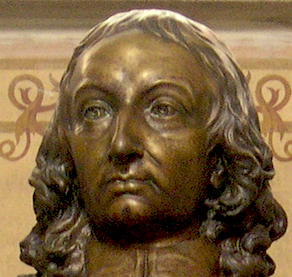
\includegraphics[width=\linewidth]{ApproxMat/pascal}
% AJR's photograph
\end{wrapfigure}
\begin{example} \label{eg:pascal}
to the left is a \(292\times277\) image of Blaise Pascal\index{Pascal, Blaise} (French mathematician, physicist, inventor, and writer, 1623--62).  
As such the image is coded as \(80\,884\)~numbers.
Let's find a good approximation to the image that uses much fewer numbers, and hence takes less storage.
That is, we effectively compress the image for storage \text{or transmission.}

\begin{solution} 
We use an \svd\ to approximate the image of Pascal to controllable levels of approximation.
For example, \cref{fig:pascalrank} shows four approximations to the image of Pascal, ranging from the hopeless (labelled ``rank~3'')  to the original image (labelled ``rank~277'').
\begin{figure}
\caption{four approximate images of Pascal ranging from the poor rank~\(3\), via the adequate rank~\(10\), the good rank~\(30\), to the original rank~\(277\).}
\label{fig:pascalrank}
\centering
\includegraphics{ApproxMat/pascalrank}
\end{figure}

\cref{pro:ai} is as follows.
\begin{itemize}
\item First obtain the image, say as a \verb|png| file (e.g., download from a website, or export a photograph). Then read the image into \script\ using 
\begin{verbatim}
rgb=imread('pascal.png');
A=mean(rgb,3);
\end{verbatim}
The \verb|imread| command sets the \(292\times277\times3\) array~\verb|rgb| to the red-green-blue values of the image data. 
Then convert into a greyscale image matrix~\verb|A| by averaging the 
red-green-blue values via the function \index{mean()@\texttt{mean()}}\verb|mean(rgb,3)| which computes the \idx{mean} over the third dimension of the array (over the three colours).

\item Compute an \svd, \(A=\usv\), of the matrix~\verb|A| with the usual command \verb|[U,S,V]=svd(A)|.
Here orthogonal~\verb|U| is \(292\times292\), diagonal \(\sloppy\verb|S|=\diag(36\,822, 7073,  \ldots,1.2859, 1.1291)\) is \(292\times277\), and orthogonal~\verb|V| is \(277\times277\).
Such matrices are far too big to record in \text{this text.}
\setbox\ajrqrbox\hbox{\qrcode{% approx Pascal
rgb=imread('pascal.png');
A=mean(rgb,3);
[U,S,V]=svd(A); 
colormap('gray')
k=10
imagesc(U(:,1:k)*S(1:k,1:k)*V(:,1:k)')
axis equal, axis off
}}%
\marginajrbox%


\begin{figure}
\caption{singular values of the image of Pascal.}
\label{fig:pascalsing}
\centering
%\includegraphics[width=\linewidth]{ApproxMat/pascalsing}
% if following revised need to add "mark size=0.6pt"
\input{ApproxMat/pascalsing.ltx}
\end{figure}
\item \cref{fig:pascalsing} plots the nonzero singular values from largest to smallest: they cover a range of five orders of magnitude (the vertical axis is logarithmic).
Choose some number~\(k\) of singular vectors to use: \(k\)~is the rank of the approximate images in \cref{fig:pascalrank}.
Guide your choice by the decrease of the singular values: as discussed later (\cref{thm:am}), for a say 1\%~error choose~\(k\) such that \(\sigma_k\approx 0.01\sigma_1\) which from the index~\(j\) axis of \cref{fig:pascalsing} is around \(k\approx 30\)\,.

\item Construct the approximate rank~\(k\) image
\begin{eqnarray*}
A_k&=&\sigma_1\uv_1\tr\vv_1+\sigma_2\uv_2\tr\vv_2+\cdots+\sigma_k\uv_k\tr\vv_k
\\&=&\verb|U(:,1:k)*S(1:k,1:k)*V(:,1:k)'|
\end{eqnarray*}

\item Let's say the rank~\(30\) image of \cref{fig:pascalrank} is the desired good approximation.  
To reconstruct it we need \(30\)~singular values \hlist\sigma{30}, \(30\)~columns \hlist\uv{30}\ of~\(U\), and \(30\)~columns \hlist\vv{30}\ of~\(V\) making a total of
\begin{equation*}
30+30\times292+30\times277=17\,100\text{ numbers}.
\end{equation*}
These \(17\,100\)~numbers are much fewer than (one fifth of) the \(292\times277=80\,884\)~numbers of the original image.
\end{itemize}
The \svd\ provides an effective flexible data compression.
\end{solution}
\end{example}











\begin{table}
\caption{As well as the \script\ commands and operations listed in 
\cref{tbl:mtlbpre,tbl:mtlbbasics,tbl:mtlbops,tbl:mtlbmops,tbl:mtlbsvd,tbl:mtlbimag}  we may invoke these functions.\index{Matlab@\textsc{Matlab}|textbf}\index{Octave|textbf}} \label{tbl:mtlbnorm}
\hrule
\begin{minipage}{\linewidth}
\begin{itemize}
\item \index{norm()@\texttt{norm()}|textbf}\verb|norm(A)| computes the \idx{matrix norm} of \cref{def:norm}, namely the largest \idx{singular value} of the matrix~\(A\).

Also recall that (\cref{tbl:mtlbpre}) \verb|norm(v)| for a vector~\verb|v| computes the \idx{length}, or \idx{magnitude}, \(\sqrt{v_1^2+v_2^2+\cdots+v_n^2}\).

%Whereas, \verb|norm(A,'fro')| computes the \idx{Frobenius norm}~\(\norm A_F\) defined such that \(\norm A_F^2=\sum_{i,j}a_{ij}^2\).

%\item \index{reshape()@\texttt{reshape()}}\verb|reshape(A,p,q)| for a \(m\times n\) matrix\slash vector~\(A\), provided \(mn=pq\)\,, generates a \(p\times q\) matrix with entries taken column-wise from~\(A\).  
%Either \(p\) or~\(q\) can be~\verb|[]| in which case \script\ uses \(p=mn/q\) or \(q=mn/p\) respectively.

\item \index{scatter()@\texttt{scatter()}|textbf}\verb|scatter(x,y,[],c)| draws a 2D scatter plot of points with coordinates in vectors~\verb|x| and~\verb|y|, each point with a colour determined by the corresponding entry of vector~\verb|c|.  

Similarly for \index{scatter3()@\texttt{scatter3()}|textbf}\verb|scatter3(x,y,z,[],c)| but in 3D.

\item \index{svds()@\texttt{svds()}|textbf}\verb|[U,S,V]=svds(A,k)| computes the \(k\)~largest \idx{singular value}s of the matrix~\(A\) in the diagonal of \(k\times k\) matrix~\(S\), and the  \(k\)~columns of~\(U\) and~\(V\) are the corresponding \idx{singular vector}s.

%Whereas \verb|[U,S,V]=svds(A,k,s)| (for \(s\geq0\)) computes the \(k\)~singular values closest to~\(s\), and the corresponding singular vectors.

\item  \index{imread()@\texttt{imread()}|textbf}\verb|imread('|filename\verb|')| typically reads an image from a file into an \(m\times n\times 3\) array of red-green-blue values. 
The values are all \idx{integer}s in the range~\([0,255]\).

\item  \index{csvread()@\texttt{csvread()}|textbf}\verb|csvread('|filename\verb|')| reads data from a file into a matrix.
When each of the \(m\)~lines in the file is \(n\)~numbers separated by commas, then the result is an \(m\times n\) matrix. 

\item \index{mean()@\texttt{mean()}|textbf}\verb|mean(A)| of an \(m\times n\) array computes the \(n\)~\idx{elements} in the \idx{row vector} of \idx{average}s (the arithmetic \idx{mean}) over each column of~\(A\).

Whereas \verb|mean(A,p)| for an \(\ell\)-dimensional array~\(A\) of dimension \(m_1\times m_2\times\cdots\times m_\ell\),  computes the \idx{mean} over the \verb|p|th~index to give an array of \idx{size} \(m_1\times\cdots\times m_{p-1}\times m_{p+1}\times\cdots\times m_\ell\).

\item \index{std()@\texttt{std()}|textbf}\verb|std(A)| of an \(m\times n\) array computes the \(n\)~elements in the \idx{row vector} of the \idx{standard deviation} over each column of~\(A\).  
That is, for each column of~\(A\), the corresponding elements of \verb|std(A)| is proportional to the \emph{spread} in values of \text{that column.}

\item For the element-by-element operations of \verb|+|, \verb|-|, \verb|.*|, \verb|./|, \verb|.^|, and so on, \index{auto-replication}\emph{\script\ auto-replicates scalars and vectors as appropriate}. 
Where this auto-replication becomes extremely useful is that if either of the matrices is \(m\times1\) or \(1\times n\), or one of each, then first its column\slash row is replicated to a matrix of size~\(m\times n\), and second the \text{operation performed.}

\emph{The general rule} is that if all the non-\(1\) sizes of the operands agree, then the dimensions of size~\(1\) in each operand are replicated as needed to match the other operand.

%\item \index{double@\texttt{double}}\verb|double(a)| converts the integers (or other data-types) in array~\verb|a| into the same size array of integer-valued real numbers that we normally use.
%\footnote{The term \emph{double} refers to the 15-digit precision of real numbers we use by default, compared to the \emph{single} precision of 7-digit real numbers used for simple purposes in, for example, graphics video cards for computers.}

%\item \index{semilogy()@\texttt{semilogy()}|textbf}\verb|semilogy(x,y,'o')| draws a point plot of~\(y\) versus~\(x\) with the vertical axis being logarithmic.

%\item \index{figure@\texttt{figure}}\verb|figure(n)| starts or restarts drawing graphics into the figure window number~\verb|n|. 

%\item \index{colormap()@\texttt{colormap()}}\verb|colormap('gray')| \script\ usually draws graphs with colour, but for many images we need greyscale; this command changes the current figure to 64~shades of grey.  

%\item \index{subplot@\texttt{subplot}}\verb|subplot(m,n,p)| notionally tiles the current figure window into  \(\verb|m|\times\verb|n|\)~rectangular tiles, and then subsequent plotting commands draw into the \verb|p|th~tile numbered row-wise.
%For example, after \verb|subplot(2,3,p)| the~\verb|p| refers to the following tiles: \(\begin{array}{|c|c|c|} \hline 1&2&3\\ \hline 4&5&6\\ \hline \end{array}\).

%\item \index{imagesc()@\texttt{imagesc()}}\verb|imagesc(A)| where \(A\)~is a \(m\times n\) matrix of values draws an \(m\times n\) image in the current figure window using the values of~\(A\) (scaled to fit) to determine the colour from the current colormap (e.g., greyscale).

\item \index{axis@\texttt{axis}|textbf}\verb|axis| sets some properties of a drawn figure:
\begin{itemize}
\item \verb|axis equal| ensures horizontal and vertical directions are scaled the same---so there is no distortion of the image;
\item \verb|axis off| means that the horizontal and vertical axes are not drawn---so the image is unadorned.
\end{itemize}


\end{itemize}
\end{minipage}
\hrule
\end{table}








\subsection{Relate matrix changes to the SVD}
\label{sec:rmmsvd}


We need to define what `best' means in the approximation \cref{pro:ai} and then show the procedure achieves this best.
%Recall diagonal matrices, orthogonal matrices and properties, rank, \svd\ factorization, and how to approximate \idx{inconsistent} right-hand side vectors.
%To proceed to understand \idx{image compression}, 
We need a measure of the \idx{magnitude} of matrices and of distances between matrices.

In linear algebra we use a pair of double vertical bars,~\(\norm{\cdot}\), to  denote the magnitude of a matrix. 
The double vertical bars avoid a notational clash with the well-established use of~\(|\cdot|\) for the determinant of a matrix (\cref{ch:ddm}).

\begin{definition} \label{def:norm} 
Let \(A\) be an \(m\times n\) matrix.  
Define the \bfidx{matrix norm} (sometimes called the \idx{spectral norm})
\begin{equation}
\norm A:=\max_{|\xv|=1}|A\xv|, 
\quad\text{equivalently }\norm A=\sigma_1
\end{equation}
the largest \idx{singular value} of the matrix~\(A\).
\footnote{Sometimes this matrix norm is more specifically called a \idx{2-norm} and correspondingly denoted by~\(\norm{A}_2\): but not in this book because at other times and places \(\norm{A}_2\)~denotes something slightly different.}
\end{definition}
%\begin{proof} 
The equivalence, that \(\max_{|\xv|=1}|A\xv|=\sigma_1\)\,, is due to the definition of the largest \idx{singular value} in the proof of the existence of an \svd\ (\cref{sec:psvdt}).
%\end{proof}



\begin{example} \label{eg:g2x2norm}
The two following \(2\times2\) matrices have the product~\(A\xv\) plotted~(red), adjoined to~\xv~(blue), for a complete range of \idx{unit vector}s~\xv\ (as in \cref{sec:iee} for eigenvectors).
From \cref{def:norm}, the norm of the matrix~\(A\) is then the \idx{length} of the longest such plotted~\(A\xv\) (this norm is a measure of the \idx{magnitude} of the matrix).
(The \script[1]\ function \index{eigshow()@\texttt{eigshow()}}\texttt{eigshow(A)}\footnote{Download for R2017b etc.} provides an interactive alternative to such static views.)

For each matrix, use the plot to roughly estimate \text{their norm.}
\begin{enumerate}[ref=\ref{eg:g2x2norm}(\alph*)]
\item\label[example]{eg:g2x2norm:a} 
\begin{figbox}{\eRose{0.5}{0.5}{-0.6}{1.2}}
\(\eAii=\begin{bmatrix} 0.5&0.5\\-0.6&1.2 \end{bmatrix}\)

\begin{solution} 
The longest \(\eAii\xv\) appear to be near the top and bottom of the plot, and appear to be a little longer than one, so estimate \(\norm{\eAii}\approx 1.3\)\,.
\aqed

\end{solution}
\end{figbox}


\item 
\begin{figbox}{\eRose{-0.7}{0.4}{0.6}{0.5}}
\(\eAii=\begin{bmatrix} {-0.7}&{0.4}\\{0.6}&{0.5} \end{bmatrix}\)

\begin{solution} 
Near the top and bottom of the plot, \(\eAii\xv\)~appears to be of length~\(0.6\).   
But the vectors pointing inwards from the right and left appear  longer at about~\(0.9\). 
So estimate \(\norm{\eAii}\approx 0.9\)\,.
\aqed

\end{solution}
\end{figbox}

\end{enumerate}
\end{example}



\begin{wrapfigure}r{0pt} \eRose1101 \end{wrapfigure}
\begin{example} 
Consider the \(2\times2\) matrix \(A=\begin{bmat} 1&1\\0&1 \end{bmat}\).
Algebraically explore products \(A\xv\) for \idx{unit vector}s~\xv, as illustrated to the right, 
and then find the \idx{matrix norm}~\(\norm{A}\).

\begin{itemize}
\item The \idx{standard unit vector} \(\ev_2=(0,1)\) has \(|\ev_2|=1\) and \(A\ev_2=(1,1)\) has length \(|A\ev_2|=\sqrt2\)\,.
Since the matrix norm is the maximum of all possible~\(|A\xv|\), so \(\norm{A}\geq|A\ev_2|=\sqrt2\approx 1.41\)\,.

\item Another unit vector is \(\xv=(\tfrac35,\tfrac45)\).
Here \(A\xv=(\tfrac75,\tfrac45)\) has length \(\sqrt{49+16}/5=\sqrt{65}/5\approx1.61\)\,.
Hence the matrix norm \(\norm{A}\geq|A\xv|\approx 1.61\)\,.

\fixwrapitem

\item To systematically find the norm, recall all unit vectors in 2D are of the form \(\xv=(\cos t,\sin t)\)\,.
Then
\begin{eqnarray*}
|A\xv|^2&=&|(\cos t+\sin t,\sin t)|^2
\\&=&(\cos t+\sin t)^2+\sin^2 t
\\&=&\cos^2 t+2\cos t\,\sin t+\sin^2t+\sin^2 t
\\&=&\tfrac32+\sin 2t-\tfrac12\cos 2t\,.
\end{eqnarray*}
This length (squared) is maximized (and minimized) for some~\(t\) determined by calculus.
Differentiating with respect to~\(t\)  leads to
\begin{equation*}
\frac{d|A\xv|^2}{dt}=2\cos2t+\sin 2t \ =0\quad\text{for stationary points.}
\end{equation*}

\begin{figbox}{\begin{tikzpicture} 
\begin{axis}[small,font=\footnotesize
  ,axis equal image, axis lines=none, xmax=1.6, xmin=-1.4 ]  
  \addplot[blue,thick] coordinates {(0,0)(1,0)(1,-2)(-1,2)(-1,0)(0,0)};
  \node[] at (axis cs:0.32,-0.15) {$2t$};
  \node[right] at (axis cs:1,-1) {$-2$};
  \node[left] at (axis cs:-1,1) {$2$};
  \node[above] at (axis cs:0.5,0) {$1$};
  \node[below] at (axis cs:-0.5,0) {$-1$};
  \node[left] at (axis cs:0.5,-1) {$\sqrt5$};
  \node[right] at (axis cs:-0.5,1) {$\sqrt5$};
\end{axis}
\end{tikzpicture}}
Rearranging this equation determines we require \(\tan 2t=-2\)\,.
The right-angle triangles, drawn to the right, illustrate that these stationary points of~\(|A\xv|^2\) occur for \(\sin 2t=\mp2/\sqrt5\) and correspondingly \(\cos2t=\pm1/\sqrt5\) (one gives a minimum and one gives the desired maximum).
Substituting these two cases gives
\begin{eqnarray*}
|A\xv|^2&=&\tfrac32+\sin 2t-\tfrac12\cos 2t
=\tfrac32\mp\tfrac2{\sqrt5}\mp\tfrac12\tfrac1{\sqrt5}
\\&=&\tfrac12(3\mp\sqrt5)
=\left(\frac{1\mp\sqrt5}2\right)^2.
\end{eqnarray*}
\end{figbox}

The plus alternative is the larger so gives the maximum, hence
\begin{equation*}
\norm{A}=\max_{|\xv|=1}|A\xv|=\frac{1+\sqrt5}2=1.6180\,.
\end{equation*}
\item Confirm with \script\ via \verb|svd([1 1;0 1])| which gives the singular values \(\sigma_1=1.6180\) and \(\sigma_2=0.6180\)\,.
Hence confirming the norm \(\norm{A}=\sigma_1=1.6180\)\,.

Alternatively, see \cref{tbl:mtlbnorm}, execute \index{norm()@\texttt{norm()}}\verb|norm([1 1;0 1])| to compute the norm \(\norm{A}=1.6180\)\,.
\aqed

\end{itemize}
\end{example}




\begin{activity}
%a=round(randn(3)*2)
%a=[1  -3  -2
%   1  -1   0
%   1   1  -2]
%[u,s,v]=svd(a)
A given \(3\times3\) matrix~\(A\) has the following products
\begin{equation*}
A\begin{bmatrix} 1\\0\\0 \end{bmatrix}
=\begin{bmatrix} 1\\1\\1 \end{bmatrix},\quad
A\begin{bmatrix} -1/3\\-2/3\\2/3 \end{bmatrix}
=\begin{bmatrix} 1/3\\1/3\\-7/3 \end{bmatrix},\quad
A\begin{bmatrix} 1\\-2\\-2 \end{bmatrix}
=\begin{bmatrix} 11\\3\\3 \end{bmatrix}.
\end{equation*}
Which of the following is the `best' statement about the norm of matrix~\(A\) (best in the sense of giving the largest valid lower bound)?
\actposs[4]{\(\|A\|\geq 3.9\)}{\(\|A\|\geq 1.7\)}{\(\|A\|\geq 2.3\)}{\(\|A\|\geq 11.7\)}
\end{activity}




\begin{example} 
\script\ readily computes the \idx{matrix norm} either via an \svd\ or using the \index{norm()@\texttt{norm()}}\verb|norm()| function directly (\cref{tbl:mtlbnorm}).
%\begin{enumerate}
%\item 
%Compute the norm of the matrix
%\(A=\begin{bmatrix} 
%   0.1&-1.3&-0.4&-0.1&-0.6\\
%   1.9&2.4&-1.8&0.2&0.8\\
%  -0.2&-0.5&-0.7&-2.5&1.1\\
%  -1.8&0.2&1.1&-1.2&1.0\\
%  -0.0&1.2&1.1&-0.1&1.7
% \end{bmatrix}\)
%\begin{solution} 
%Enter the matrix into \script\ then executing \verb|svd(A)| returns the vector of singular values
%\setbox\ajrqrbox\hbox{\qrcode{% matrix norm
%A=[0.1 -1.3 -0.4 -0.1 -0.6
%   1.9 2.4 -1.8 0.2 0.8
%  -0.2 -0.5 -0.7 -2.5 1.1
%  -1.8 0.2 1.1 -1.2 1.0
%  -0.0 1.2 1.1 -0.1 1.7]
%svd(A)
%norm(A)
%}}%
%\marginajrbox%
%\begin{equation*}\sloppy
%(4.0175,3.5044,2.6568,0.8571,0.1618),
%\end{equation*}
%so \(\norm{A}=\sigma_1=4.0175\)\,.
%Alternatively, executing \index{norm()@\texttt{norm()}}\verb|norm(A)| directly gives  \(\norm{A}=4.0175\)\,.
%\end{solution}
%
%\item 
Compute the norm of the \(4\times6\) matrix
\(B=\begin{bmat} 
0&-2&-1&-4&-5&0
\\2&0&1&-2&-6&-2
\\-2&0&4&2&3&-3
\\1&2&-4&2&1&3
\end{bmat}\)
\begin{solution} 
Enter the matrix into \script\ then executing \verb|svd(B)| returns the vector of singular values
\setbox\ajrqrbox\hbox{\qrcode{% matrix norm
B=[0 -2 -1 -4 -5 0
 2 0 1 -2 -6 -2
 -2 0 4 2 3 -3
 1 2 -4 2 1 3]
svd(B)
norm(B)
}}%
\marginajrbox%
\(\sloppy(10.1086,7.6641,3.2219,0.8352)\),
so \(\norm{B}=\sigma_1=10.1086\)\,.
Alternatively, executing \index{norm()@\texttt{norm()}}\verb|norm(B)| directly gives  \(\norm{B}=10.1086\)\,.
\end{solution}

%\end{enumerate}
\end{example}










The \cref{def:norm} of the \idx{magnitude}\slash norm of a matrix may appear a little strange. 
But, in addition to some other marvellously useful properties, the norm nonetheless has all the familiar properties of a \idx{magnitude}\slash length.
Recall from \cref{ch:v} that \text{for vectors:}
\begin{itemize}
\item \(|\vv|=0\) if and only if \(\vv=\ov\) (\cref{thm:veclen0});
\item \(|\uv\pm\vv|\leq|\uv|+|\vv|\) (the \idx{triangle inequality} of \cref{thm:triscal});
\item \(|t\vv|=|t|\cdot|\vv|\) (\cref{thm:triscal}).
\end{itemize}
Analogous `magnitude' properties hold for the matrix norm as established in the next theorem.




\begin{theorem}[\idx{matrix norm} properties] \label{thm:norm} 
For every \(m\times n\) real matrix~\(A\):
\begin{enumerate}[ref=\ref{thm:norm}(\alph*)]
\item\label[theorem]{thm:norm:iii} \(\norm A=0\) if and only if \(A=O_{m\times n}\)\,;
\item\label[theorem]{thm:norm:vi} \(\norm{I_n}=1\)\,;
\item\label[theorem]{thm:norm:iv} \(\norm {A\pm B}\leq\norm{A}+\norm B\), for every \(m\times n\) matrix~\(B\), is like a \idx{triangle inequality} (\cref{thm:triscalc});
\item\label[theorem]{thm:norm:v} \(\norm{tA}=|t|\cdot\norm{A}\)\,;
\item\label[theorem]{thm:norm:i} \(\norm A=\norm{\tr A}\)\,;
\item\label[theorem]{thm:norm:ii} \(\norm{Q_mA}=\norm A=\norm{AQ_n}\) for every \(m\times m\) \idx{orthogonal matrix}~\(Q_m\) and every \(n\times n\) \idx{orthogonal matrix}~\(Q_n\);
\item\label[theorem]{thm:norm:viii} \(|A\xv|\leq\norm{A}\cdot|\xv|\) for all \(\xv\in\RR^n\), is like a \idx{Cauchy--Schwarz inequality} (\cref{thm:triscalb}), as is the next;
\item\label[theorem]{thm:norm:vii} \(\norm{AB}\leq\norm A\norm B\) for every \(n\times p\) matrix~\(B\).
\end{enumerate}
\end{theorem}
\begin{proof}  Alternative proofs to the following may be invoked (\cref{ex:norm}).
Where necessary in the following, let matrix~\(A\) have the \svd\ \(A=\usv\).
\begin{description}
\item[\ref{thm:norm:iii}]
If \(A=O_{m\times n}\) \,,
then from \cref{def:norm} 
\begin{equation*}
\norm A=\max_{|\xv|=1}|O\xv|
=\max_{|\xv|=1}|\ov|=\max_{|\xv|=1}0=0\,.
\end{equation*}
Conversely, if \(\norm A=0\)\,, then the largest singular value \(\sigma_1=0\) (\cref{def:norm}), which implies that all singular values are zero, so the matrix~\(A\) has an \svd\ of the form \(A=UO_{m\times n}\tr V\)\,, which reduces to \(A=O_{m\times n}\)\,.

\item[\ref{thm:norm:vi}] From \cref{def:norm}, 
\begin{equation*}
\norm{I_n}=\max_{|\xv|=1}|I_n\xv|
=\max_{|\xv|=1}|\xv|
=\max_{|\xv|=1}1
=1\,.
\end{equation*}


\item[\ref{thm:norm:iv}]
Using \cref{def:norm} at the first and last steps:
\begin{eqnarray*}
\norm{A\pm B}
&=&\max_{|\xv|=1}|(A\pm B)\xv|
=\max_{|\xv|=1}|A\xv\pm B\xv|
\quad(\text{by distributivity})
\\&\leq&\max_{|\xv|=1}(|A\xv|+ |B\xv|)
\quad(\text{by triangle inequality})
\\&&{}\leq\max_{|\xv|=1}|A\xv|+ \max_{|\xv|=1}|B\xv|
=\norm A+ \norm B\,.
\end{eqnarray*}

\item[\ref{thm:norm:v}]
Using \cref{def:norm},
\begin{eqnarray*}
\norm{tA}
&=&\max_{|\xv|=1}|(tA)\xv|
=\max_{|\xv|=1}|t(A\xv)|
\quad(\text{by associativity})
\\&=&\max_{|\xv|=1}|t||A\xv|
\quad(\text{by \cref{thm:triscal}})
\\&=&|t|\max_{|\xv|=1}|A\xv|
=|t|\cdot\norm A\,.
\end{eqnarray*}

\item[\ref{thm:norm:i}]
Recall that the transpose~\(\tr A\) has an \svd\ \(\tr A=\tr{(\usv)}=V\tr S\tr U\), and so has the same singular values as~\(A\).
So the largest singular value of~\(\tr A\) is the same as that of~\(A\).
Hence \(\norm A=\norm{\tr A}\).

\item[\ref{thm:norm:ii}]
Recall that multiplication by an orthogonal matrix is a rotation\slash reflection and so does not change lengths (\cref{thm:orthog:iv}): correspondingly, it also does not change the norm of a matrix as established here.

Now \(Q_mA=Q_m(\usv)=(Q_mU)S\tr V\).
But \(Q_mU\)~is an orthogonal matrix (\cref{ex:orthoprod}),
so \((Q_mU)S\tr V\) is an \svd\ for~\(Q_mA\) and so has the same singular values as those in~\(S\).
Hence, \(\norm{Q_mA}=\sigma_1=\norm A\)\,.

Also, using~\ref{thm:norm:i} twice: \(\norm{AQ_n}=\norm{\tr{(AQ_n)}}=\norm{\tr Q_n\tr A}=\norm{\tr A}=\norm A\)\,.

\item[\ref{thm:norm:viii}]
Split into two cases.
In the case \(\xv=\ov\), then \(|A\xv|=|A\ov|=|\ov|=0\) whereas \(\norm{A}|\xv|=\norm{A}|\ov|=\norm A0=0\)\,, so \(|A\xv|\leq\norm{A}|\xv|\).
Alternatively, in the case \(\xv\neq\ov\), then we write \(\xv=\hat{\xv}|\xv|\) for unit vector \(\hat{\xv}=\xv/|\xv|\)  so that
\begin{eqnarray*}
|A\xv|&=&\big|A\hat{\xv}|\xv|\big|
=|A\hat{\xv}||\xv| \quad(\text{as }|\xv|\text{ is a scalar})
\\&\leq&\big(\max_{|\hat{\xv}|=1}|A\hat{\xv}|\big)|\xv|
\quad(\text{as }\hat{\xv}\text{ is a unit vector})
\\&&{}=\norm{A}|\xv|\quad(\text{by \cref{def:norm}})
\end{eqnarray*}


\item[\ref{thm:norm:vii}] See \cref{ex:norm:vii}. 
\end{description}
\end{proof}




Since the matrix norm has these familiar properties of a measure of \idx{magnitude}, we use the matrix norm to measure the `\idx{distance}' between matrices.

\begin{example} 
\begin{enumerate}
\item Use the \idx{matrix norm} to estimate the `\idx{distance}' between matrices
\begin{equation*}
B=\begin{bmatrix} {-0.7}&{0.4}\\{0.6}&{0.5} \end{bmatrix}
\quad\text{and}\quad
C=\begin{bmatrix} -0.2&0.9\\0&1.7 \end{bmatrix}.
\end{equation*}
\begin{solution} 
The `distance' between matrices~\(B\) and~\(C\) is, via the matrix~\(A\) of \cref{eg:g2x2norm:a} and its estimated norm,
\begin{equation*}
\norm{C-B}=\left\|\begin{bmatrix} 0.5&0.5\\-0.6&1.2 \end{bmatrix}\right\|
=\norm{A}\approx 1.3\,.
\end{equation*} 
\end{solution}


\item Find the distances between the matrix
\begin{equation*}
A=\begin{bmatrix} 10&2\\5&11 \end{bmatrix}
\quad\text{and }B=\begin{bmatrix} 4&-4\\-3&3 \end{bmatrix},
\quad\text{and } A_1=\begin{bmatrix} 6&6\\8&8 \end{bmatrix}.
\end{equation*}
Recall from \cref{eg:2by2svd} that the matrix~\(A\) has an \svd\ of
\begin{equation*}
\usv=\begin{bmatrix} \frac35&-\frac45\\\frac45&\frac35 \end{bmatrix}
\begin{bmatrix} 10\sqrt2&0\\0&5\sqrt2 \end{bmatrix}
\tr{\begin{bmatrix} \frac1{\sqrt2}&-\frac1{\sqrt2}\\ \frac1{\sqrt2}&\frac1{\sqrt2} \end{bmatrix}}.
\end{equation*}
\begin{enumerate}
\item Find \(\norm{A-B}\) for the rank one matrix 
\begin{equation*}
B=\sigma_2\uv_2\tr{\vv_2}
=5\sqrt2\begin{bmatrix} -\frac45\\\frac35 \end{bmatrix}
\begin{bmatrix} -\frac1{\sqrt2}&\frac1{\sqrt2} \end{bmatrix}
=\begin{bmatrix} 4&-4\\-3&3 \end{bmatrix}.
\end{equation*}
\begin{solution} 
Let's write matrix
\begin{equation*}
B=\begin{bmatrix} \frac35&-\frac45\\\frac45&\frac35 \end{bmatrix}
\begin{bmatrix} 0&0\\0&5\sqrt2 \end{bmatrix}
\tr{\begin{bmatrix} \frac1{\sqrt2}&-\frac1{\sqrt2}\\ \frac1{\sqrt2}&\frac1{\sqrt2} \end{bmatrix}}
=U\begin{bmatrix} 0&0\\0&5\sqrt2 \end{bmatrix}\tr V\,.
\end{equation*}
Then the difference is
\begin{eqnarray*}
A-B&=&U\begin{bmatrix} 10\sqrt2&0\\0&5\sqrt2 \end{bmatrix}\tr V
-U\begin{bmatrix} 0&0\\0&5\sqrt2 \end{bmatrix}\tr V
\\&=&U\left(\begin{bmatrix} 10\sqrt2&0\\0&5\sqrt2 \end{bmatrix}
-\begin{bmatrix} 0&0\\0&5\sqrt2 \end{bmatrix}\right)\tr V
=U\begin{bmatrix} 10\sqrt2&0\\0&0 \end{bmatrix}\tr V\,.
\end{eqnarray*}
This last expression is an \svd\ for \(A-B\) with singular values \(10\sqrt2\) and~\(0\), so by \cref{def:norm} its norm \(\norm{A-B}=\sigma_1=10\sqrt2\)\,.
\end{solution}

\item Find \(\norm{A-A_1}\) for the rank one matrix 
\begin{equation*}
A_1=\sigma_1\uv_1\tr{\vv_1}
=10\sqrt2\begin{bmatrix} \frac35\\\frac45 \end{bmatrix}
\begin{bmatrix} \frac1{\sqrt2}&\frac1{\sqrt2} \end{bmatrix}
=\begin{bmatrix} 6&6\\8&8 \end{bmatrix}.
\end{equation*}
\begin{solution} 
Let's write matrix
\begin{equation*}
A_1=\begin{bmatrix} \frac35&-\frac45\\\frac45&\frac35 \end{bmatrix}
\begin{bmatrix} 10\sqrt2&0\\0&0 \end{bmatrix}
\tr{\begin{bmatrix} \frac1{\sqrt2}&-\frac1{\sqrt2}\\ \frac1{\sqrt2}&\frac1{\sqrt2} \end{bmatrix}}
=U\begin{bmatrix} 10\sqrt2&0\\0&0 \end{bmatrix}\tr V\,.
\end{equation*}
Then the difference is
\begin{eqnarray*}
A-A_1&=&U\begin{bmatrix} 10\sqrt2&0\\0&5\sqrt2 \end{bmatrix}\tr V
-U\begin{bmatrix} 10\sqrt2&0\\0&0 \end{bmatrix}\tr V
\\&=&U\left(\begin{bmatrix} 10\sqrt2&0\\0&5\sqrt2 \end{bmatrix}
-\begin{bmatrix} 10\sqrt2&0\\0&0 \end{bmatrix}\right)\tr V
=U\begin{bmatrix} 0&0\\0&5\sqrt2 \end{bmatrix}\tr V\,.
\end{eqnarray*}
This last expression is an \svd\ for \(A-A_1\) with singular values \(5\sqrt2\) and~\(0\), albeit out of order, so by \cref{def:norm} the norm \(\norm{A-A_1}\) is the largest singular value which here is~\(5\sqrt2\).
\end{solution}
\end{enumerate}
Out of these two matrices, \(A_1\) and~\(B\), the matrix~\(A_1\) is `closer' to~\(A\) as \(\norm{A-A_1}=5\sqrt2<10\sqrt2=\norm{A-B}\).
\end{enumerate}
\end{example}




\begin{activity}
Which of the following matrices is \emph{not} a \idx{distance} one from the matrix \(F=\begin{bmatrix} 9&-1\\1&5 \end{bmatrix}\)?
\actposs[4]{\(\begin{bmatrix} 8&-2\\2&4 \end{bmatrix}\)}
{\(\begin{bmatrix} 8&-1\\1&5 \end{bmatrix}\)}
{\(\begin{bmatrix} 9&-1\\1&6 \end{bmatrix}\)}
{\(\begin{bmatrix} 10&-1\\1&6 \end{bmatrix}\)}
\end{activity}




\begin{reduce}
\begin{example} 
From \cref{eg:bullseyemat}, recall the `\idx{bulls eye}' matrix
\begin{equation*}
A=\begin{bmat} 0&1&1&1&0
\\1&0&0&0&1
\\1&0&1&0&1
\\1&0&0&0&1
\\0&1&1&1&0 \end{bmat},
\end{equation*}
and its rank two and three approximations~\(A_2\) and~\(A_3\).
Find \(\norm{A-A_2}\) and~\(\norm{A-A_3}\).
\begin{solution} 
\cref{eg:bullseyemat} found \(A_3=A\) hence \(\norm{A-A_3}=\norm{O_5}=0\)\,.

Although \(\norm{A-A_2}\) is nontrivial, finding it is straightforward using \svd{}s.
Recall that, from the given \svd\ \(A=\usv\),
\begin{eqnarray*}
A_2&=&\sigma_1\uv_1\tr\vv_1+\sigma_2\uv_2\tr\vv_2
=\sigma_1\uv_1\tr\vv_1+\sigma_2\uv_2\tr\vv_2+0\uv_3\tr\vv_3+0\uv_4\tr\vv_4+0\uv_5\tr\vv_5
\\&=&U\begin{bmatrix} \sigma_1&0&0&0&0
\\0&\sigma_2&0&0&0
\\0&0&0&0&0
\\0&0&0&0&0
\\0&0&0&0&0 \end{bmatrix}\tr V.
\end{eqnarray*}
Hence the difference
\begin{eqnarray*}
A-A_2&=&U\begin{bmatrix} \sigma_1&0&0&0&0
\\0&\sigma_2&0&0&0
\\0&0&\sigma_3&0&0
\\0&0&0&\sigma_4&0
\\0&0&0&0&\sigma_5 \end{bmatrix}\tr V
-U\begin{bmatrix} \sigma_1&0&0&0&0
\\0&\sigma_2&0&0&0
\\0&0&0&0&0
\\0&0&0&0&0
\\0&0&0&0&0 \end{bmatrix}\tr V
\\&=&U\begin{bmatrix} 0&0&0&0&0
\\0&0&0&0&0
\\0&0&\sigma_3&0&0
\\0&0&0&\sigma_4&0
\\0&0&0&0&\sigma_5 \end{bmatrix}\tr V.
\end{eqnarray*}
This last expression is an \svd\ for \(A-A_2\), albeit with the singular values out of order, with singular values of~\(0\), \(0\), \(\sigma_3=0.64\), and \(\sigma_4=\sigma_5=0\)\,.
The largest of these singular values,~\(\sigma_3\), gives the norm \(\norm{A-A_2}=0.64\) \twodp.

To be discussed later, the relative error in the approximate~\(A_2\) is \(\norm{A-A_2}/\norm{A} =\sigma_3/\sigma_1 =0.64/2.68 =0.24 =24\%\) \twodp.
\end{solution}
\end{example}
\end{reduce}








\begin{theorem}[Eckart--Young] \label{thm:am}
Let \(A\) be any \(m\times n\) matrix of \(\rank r\) with \svd\ \(A=\usv\).  
Then for every \(k< r\) the matrix
\begin{equation}
A_k:=US_k\tr V =\sigma_1\uv_1\tr\vv_1 +\sigma_2\uv_2\tr\vv_2+\cdots +\sigma_k\uv_k\tr\vv_k
\label{eq:rankkA}
\end{equation}
where \(S_k:=\diag(\hlist\sigma k,0,\ldots,0)\), is a \emph{closest} \idx{rank}~\(k\) matrix approximating~\(A\), in the \idx{matrix norm}.
The \idx{distance} between~\(A\) and~\(A_k\) is \(\norm{A-A_k}=\sigma_{k+1}\)\,.
\end{theorem}

That is, obtain a closest rank~\(k\) matrix~\(A_k\) by `setting' the \idx{singular value}s \(\sigma_{k+1}=\cdots=\sigma_r=0\) from an \svd\ for~\(A\).

\begin{proof} 
As a prelude to this difficult proof, let's establish the distance between~\(A\) and~\(A_k\). 
Using their \svd{}s,
\begin{eqnarray*}
A-A_k&=&\usv-US_k\tr V=U(S-S_k)\tr V
\\&=&U\diag(0,\ldots,0,\sigma_{k+1},\ldots,\sigma_r,0,\ldots,0)\tr V,
\end{eqnarray*}
and so \(A-A_k\) has largest singular value~\(\sigma_{k+1}\).
Then from \cref{def:norm}, \(\norm{A-A_k}=\sigma_{k+1}\)\,.

Now let's use \idx{contradiction} to prove there is no matrix of rank~\(k\) closer to~\(A\) when using \(\norm{\cdot}\) to measure matrix distances \cite[p.36]{Trefethen1997}.
Assume there is some \(m\times n\) matrix~\(B\) with \(\rank B\leq k\) \emph{and} \(B\)~is closer to~\(A\) than is~\(A_k\), that is, \(\norm{A-B}<\norm{A-A_k}\).
First, the Rank \cref{thm:rank} asserts the \idx{nullspace} of~\(B\) has dimension \(\nullity B =n-\rank B\geq n-k\) as  \(\rank B\leq k\)\,.
For every \(\wv\in\Null B\)\,,  as \(B\wv=\ov\)\,,  \(A\wv=A\wv-B\wv=(A-B)\wv\)\,. 
Then
\begin{eqnarray*}
|A\wv|&=&|(A-B)\wv|
\\&\leq&\norm{A-B}|\wv| 
\quad(\text{by \cref{thm:norm:viii}})
\\&&{}<\norm{A-A_k}|\wv|
\quad(\text{by assumption})
\\&&\phantom{{}<}{}=\sigma_{k+1}|\wv|
\end{eqnarray*}
That is, under the assumption there exists an (at least) \((n-k)\)-dimensional \idx{subspace} in which \(|A\wv|<\sigma_{k+1}|\wv|\)\,.

Second, consider \emph{any} vector~\vv\ in the \((k+1)\)-dimensional subspace \(\Span\{\hlist\vv{k+1}\}\).
Say \(\vv=\lincomb c\vv{k+1}=V\cv\) for some vector of coefficients \(\cv=(\hlist c{k+1},0,\ldots,0)\in\RR^n\).
Then
\begin{eqnarray*}
|A\vv|&=&|\usv V\cv|
=|US\cv| \quad(\text{as }\tr VV=I)
\\&=&|S\cv| \quad(\text{as \(U\) is orthogonal})
\\&=&\big|(\sigma_1c_1,\sigma_2c_2,\ldots,\sigma_{k+1}c_{k+1},0,\ldots,0)\big|
\\&=&\sqrt{\sigma_1^2c_1^2+\sigma_2^2c_2^2+\cdots+\sigma_{k+1}^2c_{k+1}^2}
\\&\geq&\sqrt{\sigma_{k+1}^2c_1^2+\sigma_{k+1}^2c_2^2+\cdots+\sigma_{k+1}^2c_{k+1}^2}
\\&&{}=\sigma_{k+1}\sqrt{c_1^2+c_2^2+\cdots+c_{k+1}^2}
\\&&{}=\sigma_{k+1}|\cv|
=\sigma_{k+1}|V\cv|\quad(\text{as \(V\) is orthogonal})
\\&&{}=\sigma_{k+1}|\vv|.
\end{eqnarray*}
That is, there exists a \((k+1)\)-dimensional \idx{subspace} in which \(|A\vv|\geq\sigma_{k+1}|\vv|\)\,.

Lastly, since the sum of the dimensions of these two subspaces of~\(\RR^n\) is at least \((n-k)+(k+1)>n\), there must be a nonzero vector, say~\uv, lying in both.
So for this~\uv, simultaneously \(|A\uv|<\sigma_{k+1}|\uv|\) and \(|A\uv|\geq\sigma_{k+1}|\uv|\)\,.
These two statements contradict each other.
Hence the assumption is wrong: there is no rank~\(k\) matrix more closely approximating~\(A\) than~\(A_k\).
\end{proof}


\begin{wrapfigure}r{0pt} \input{ApproxMat/R.ltx} \end{wrapfigure}
\begin{example}[the letter \texttt{R}] 
In digital displays with low resolution, letters and numbers are displayed with noticeable \idx{pixel pattern}s: for example, the letter~\verb|R| is pixellated to the right.
Let's see how such \idx{pixel pattern}s are best approximated by matrices of different ranks.
(This example is illustrative: it is not a practical \idx{image compression} since the required singular vectors are more complicated than a small-sized pattern \text{of pixels.)}
\begin{solution} 
Use \cref{pro:ai}.
First, form and enter into \script\ the \(7\times5\) matrix of the pixel pattern as illustrated above-right
\begin{equation*}
R=\begin{bmat} 1&1&1&1&0
\\1&0&0&0&1
\\1&0&0&0&1
\\1&1&1&1&0
\\1&0&1&0&0
\\1&0&0&1&0
\\1&0&0&0&1 \end{bmat}.
\end{equation*}
Second, compute an \svd\ via \verb|[U,S,V]=svd(R)| to find \twodp
\begin{verbatim}
U =
  -0.53   0.38  -0.00  -0.29  -0.70  -0.06  -0.07
  -0.28  -0.49   0.00  -0.13   0.10  -0.69  -0.42
  -0.28  -0.49  -0.00  -0.13  -0.02   0.72  -0.39
  -0.53   0.38  -0.00  -0.29   0.70   0.06   0.07
  -0.32   0.03  -0.71   0.63  -0.00  -0.00  -0.00
  -0.32   0.03   0.71   0.63  -0.00   0.00   0.00
  -0.28  -0.49  -0.00  -0.13  -0.08  -0.02   0.81
S =
   3.47      0      0      0      0
      0   2.09      0      0      0
      0      0   1.00      0      0
      0      0      0   0.75      0
      0      0      0      0   0.00
      0      0      0      0      0
      0      0      0      0      0
V =
  -0.73  -0.32   0.00   0.40  -0.45
  -0.30   0.36  -0.00  -0.76  -0.45
  -0.40   0.37  -0.71   0.07   0.45
  -0.40   0.37   0.71   0.07   0.45
  -0.24  -0.70  -0.00  -0.50   0.45
\end{verbatim}
\setbox\ajrqrbox\hbox{\qrcode{% approx bulls eye image
R=[ 1 1 1 1 0
    1 0 0 0 1
    1 0 0 0 1
    1 1 1 1 0
    1 0 1 0 0
    1 0 0 1 0
    1 0 0 0 1 ]
[U,S,V]=svd(R)
R2=U(:,1:2)*S(1:2,1:2)*V(:,1:2)'
}}%
\marginajrbox%
The singular values are \(\sigma_1=3.47\), \(\sigma_2=2.09\), \(\sigma_3=1.00\), \(\sigma_4=0.75\) and \(\sigma_5=0\)\,.
Four successively better approximations to the image are the following.
\begin{itemize}
\item  
\begin{figbox}{\input{ApproxMat/R1.ltx}}
The coarsest approximation is \(R_1=\sigma_1\uv_1\tr\vv_1\), that is
{\small\begin{equation*}
R_1=3.47
\begin{bmatrix} -0.53\\-0.28\\-0.28\\-0.53\\-0.32\\-0.32\\-0.28 \end{bmatrix}
\begin{bmatrix} -0.73&-0.30&-0.40&-0.40&-0.24 \end{bmatrix}.
\end{equation*}}%
Compute with \verb|R1=U(:,1)*S(1,1)*V(:,1)'| to find \twodp, as illustrated above,
\end{figbox}
\begin{verbatim}
R1 =
   1.34   0.55   0.72   0.72   0.44
   0.71   0.29   0.39   0.39   0.24
   0.71   0.29   0.39   0.39   0.24
   1.34   0.55   0.72   0.72   0.44
   0.83   0.34   0.45   0.45   0.27
   0.83   0.34   0.45   0.45   0.27
   0.71   0.29   0.39   0.39   0.24
\end{verbatim}
This has difference \(\norm{R-R_1}=\sigma_2=2.09\) which at~60\% of~\(\sigma_1\) is large: indeed the letter~\verb|R| is not recognizable.

\item 
\begin{figbox}{\input{ApproxMat/R2.ltx}}
Computing \verb|R2=U(:,1:2)*S(1:2,1:2)*V(:,1:2)'| finds the second approximation \(R_2=\sigma_1\uv_1\tr\vv_1+\sigma_2\uv_2\tr\vv_2\)
is \twodp, as illustrated,
\end{figbox}
\begin{verbatim}
R2 =
   1.09   0.83   1.02   1.02  -0.11
   1.04  -0.07   0.01   0.01   0.95
   1.04  -0.07   0.01   0.01   0.95
   1.09   0.83   1.02   1.02  -0.11
   0.81   0.36   0.47   0.47   0.24
   0.81   0.36   0.47   0.47   0.24
   1.04  -0.07   0.01   0.01   0.95
\end{verbatim}
This has difference \(\norm{R-R_2}=\sigma_3=1.00\) which at~29\% of~\(\sigma_1\) is large: but one can begin to imagine the letter~\verb|R| in the image.

 
\item 
\begin{figbox}{\input{ApproxMat/R3.ltx}}
The third approximation is 
\begin{equation*}
R_3=\sigma_1\uv_1\tr\vv_1 +\sigma_2\uv_2\tr\vv_2 +\sigma_3\uv_3\tr\vv_3\,.
\end{equation*}
Compute with \verb|R3=U(:,1:3)*S(1:3,1:3)*V(:,1:3)'| to find \twodp, as illustrated, 
\end{figbox}
\begin{verbatim}
R3 =
   1.09   0.83   1.02   1.02  -0.11
   1.04  -0.07   0.01   0.01   0.95
   1.04  -0.07   0.01   0.01   0.95
   1.09   0.83   1.02   1.02  -0.11
   0.81   0.36   0.97  -0.03   0.24
   0.81   0.36  -0.03   0.97   0.24
   1.04  -0.07   0.01   0.01   0.95
\end{verbatim}
This has difference \(\norm{R-R_3}=\sigma_4=0.75\) which at~22\% of~\(\sigma_1\) is moderate and one can see the letter~\verb|R| emerging.
 
\item 
\begin{figbox}{\input{ApproxMat/R4.ltx}}
The fourth approximation is 
\begin{equation*}
R_4=\sigma_1\uv_1\tr\vv_1+\sigma_2\uv_2\tr\vv_2+\cdots+\sigma_4\uv_4\tr\vv_4\,.
\end{equation*}
Compute with \verb|R4=U(:,1:4)*S(1:4,1:4)*V(:,1:4)'| to find \twodp, as illustrated, 
\end{figbox}
\begin{verbatim}
R4 =
   1.00   1.00   1.00   1.00  -0.00
   1.00   0.00  -0.00   0.00   1.00
   1.00   0.00  -0.00  -0.00   1.00
   1.00   1.00   1.00   1.00  -0.00
   1.00  -0.00   1.00   0.00  -0.00
   1.00  -0.00  -0.00   1.00   0.00
   1.00   0.00  -0.00  -0.00   1.00
\end{verbatim}
This has difference \(\norm{R-R_4}=\sigma_5=0.00\) and so \(R_4\)~exactly reproduces~\verb|R|.
\aqed
 
\end{itemize}
\end{solution}
\end{example}




\begin{activity}
A given image has \idx{singular value}s \(12.74\), \(8.38\), \(3.06\), \(1.96\), \(1.08\), \ldots. 
What rank approximation has a relative error of just a little less than~25\%?
\actposs[4]2134
\end{activity}





\begin{example} 
Recall \cref{eg:pascal} approximated the image of Blaise \idx{Pascal} with various rank~\(k\) approximations, and that
these approximations came from an \svd\ of the image.
Let the image be denoted by matrix~\(A\).
From \cref{fig:pascalsing} the largest \idx{singular value} of the image is \(\norm A=\sigma_1\approx37\,000\)\,.
\begin{itemize}
\item From  \cref{thm:am}, the rank~3 approximation in \cref{fig:pascalrank} is a \idx{distance} \(\norm{A-A_3}=\sigma_4\approx 3\,200\) (from \cref{fig:pascalsing}) away from the image.  
That is, image~\(A_3\) has a \idx{relative error} roughly \(3\,200/37\,000\approx 9\%\).
\item From  \cref{thm:am}, the rank~10 approximation in \cref{fig:pascalrank} is a distance \(\norm{A-A_{10}}=\sigma_{11}\approx 1\,500\) (from \cref{fig:pascalsing}) away from the image.  
That is, image~\(A_{10}\) has a relative error roughly \(1\,500/37\,000 \approx 4\%\). 
\item From  \cref{thm:am}, the rank~30 approximation in \cref{fig:pascalrank} is a distance \(\norm{A-A_{30}}=\sigma_{31}\approx 600\) (from \cref{fig:pascalsing}) away from the image.  
That is, image~\(A_{30}\) has a relative error roughly \(600/37\,000 \approx 2\%\). 
\end{itemize}
\end{example}


\begin{comment}
Could introduce the Frobenius norm here, but would confuse some, and there is no need.  If anywhere, then perhaps better in the general vector space chapter.
\end{comment}
%\begin{definition} \label{def:normf} 
%Let \(A\) be an \(m\times n\) matrix, with columns \(\begin{bmatrix} \av_1&\av_2&\cdots&\av_n \end{bmatrix}\).  
%Define the \bfidx{Frobenius norm}~\normf A\ as the square root of the sum of the squares of all its entries:
%%%%As of Mar 2016, do not use $\sum$ anywhere
%\begin{equation*}
%\normf A^2:=\sum_{i=1}^{m}\sum_{j=1}^{n} a_{ij}^2
%=\sum_{j=1}^n |\av_j|^2
%=\trace(\tr AA)
%,
%\end{equation*}
%where the \bfidx{trace} of a matrix is the sum of its diagonal entries.
%\end{definition}
%\begin{proof} %They are the same straightforwardly from definition.
%\begin{itemize}
%\item The first identity is the square of the definition.
%\item To establish the second identity 
%\(\sum_{i=1}^{m}\sum_{j=1}^{n} a_{ij}^2
%=\sum_{j=1}^n |\av_j|^2\) recall the column vectors \(\av_j=(a_{1j},a_{2j},\ldots,a_{mj})\).
%Consequently \(|\av_j|^2=\sum_{i=1}^m a_{ij}^2\), and hence
%\(\sum_{j=1}^n |\av_j|^2=\sum_{j=1}^n\sum_{i=1}^m a_{ij}^2=\sum_{i=1}^{m}\sum_{j=1}^{n} a_{ij}^2 \) as required.
%\item Now establish the third identity \(\sum_{j=1}^n |\av_j|^2
%=\trace(\tr AA)\).
%Recall from the proof of the Orthogonal \cref{thm:orthog} that the product
%\begin{eqnarray*}
%\tr AA
%&=&\begin{bmatrix} \tr\av_1\\\tr\av_2\\\vdots\\\tr\av_n \end{bmatrix}
%\begin{bmatrix} \av_1&\av_2&\cdots&\av_n \end{bmatrix}
%\\&=&\begin{bmatrix} \tr\av_1\av_1&\tr\av_1\av_2&\cdots&\tr\av_1\av_n 
%\\ \tr\av_2\av_1&\tr\av_2\av_2&\cdots&\tr\av_2\av_n 
%\\\vdots&&\ddots&\vdots
%\\ \tr\av_n\av_1&\tr\av_n\av_2&\cdots&\tr\av_n\av_n \end{bmatrix}
%\\&=&\begin{bmatrix} \av_1\cdot\av_1&\av_1\cdot\av_2&\cdots&\av_1\cdot\av_n 
%\\ \av_2\cdot\av_1&\av_2\cdot\av_2&\cdots&\av_2\cdot\av_n 
%\\\vdots&&\ddots&\vdots
%\\ \av_n\cdot\av_1&\av_n\cdot\av_2&\cdots&\av_n\cdot\av_n \end{bmatrix}
%\end{eqnarray*}
%Hence the trace, the sum of the diagonal entries, is
%\(\trace(\tr AA)=\sum_{j=1}^n \av_j\cdot\av_j
%=\sum_{j=1}^n|\av_j|^2\) as required.
%\end{itemize}
%\end{proof}
%
%\begin{theorem} \label{thm:normf} 
%Let \(A\) be an \(m\times n\) matrix, and \(Q\) be an \(m\times m\) \idx{orthogonal matrix}:
%\begin{enumerate}
%\item\label[theorem]{thm:normf:i} \(\normf A=\normf{\tr A}\)\,;
%\item\label[theorem]{thm:normf:ii} \(\normf{QA}=\normf A\)\,.
%\end{enumerate}
%\end{theorem}
%\begin{proof} %Immediate from definition, and 
%\begin{itemize}
%\item[\ref{thm:normf:i}.]
%Consider
%\begin{equation*}
%\normf{\tr A}^2
%=\sum_{i=1}^{n}\sum_{j=1}^{m}(\tr A)_{ij}^2
%=\sum_{i=1}^{n}\sum_{j=1}^{m} a_{ji}^2
%=\sum_{i=1}^{m}\sum_{j=1}^{n} a_{ij}^2
%=\normf{A}^2.
%\end{equation*}
%
%\item[\ref{thm:normf:ii}.]
%Use the columns of matrix \(A=\begin{bmatrix} \av_1&\av_2&\cdots&\av_n \end{bmatrix}\) as then \(QA=\begin{bmatrix} Q\av_1&Q\av_2&\cdots&Q\av_n \end{bmatrix}\).
%From \cref{def:normf}, and remembering that multiplication by an orthogonal matrix~\(Q\) does not change lengths (\cref{thm:orthog}),
%\begin{equation*}
%\normf{QA}^2
%=\sum_{j=1}^n |Q\av_j|^2
%=\sum_{j=1}^n |\av_j|^2
%=\normf{A}^2.
%\end{equation*}
%\end{itemize}
%\end{proof}
%
%\begin{theorem} \label{thm:normfsvd} 
%Let \(A\) be an \(m\times n\) matrix of \(\rank r\) and with \idx{singular value}s \hlist\sigma r\,.
%Then \(\normf A=\sqrt{\sigma_1^2+\sigma_2^2+\cdots+\sigma_r^2}\).
%\end{theorem}
%\begin{proof} 
%Consider an \svd\ \(A=\usv\) and use \cref{thm:normf} thrice:
%\(\normf{A}
%=\normf{\usv}
%=\normf{S\tr V}
%=\normf{\tr{(S\tr V)}}
%=\normf{V\tr S}
%=\normf{\tr S}
%=\sqrt{\sigma_1^2+\sigma_2^2+\cdots+\sigma_r^2}
%\)
%as all other elements of diagonal~\(S\) are zero.
%\end{proof}
%
%\begin{theorem} \label{thm:am}
%Let \(A\) be an \(m\times n\) matrix of \(\rank r\) with \svd\ \(A=\usv\).  
%Then for every \(k<r\) the closest rank~\(k\) matrix approximating~\(A\), in the \idx{Frobenius norm}, is
%\begin{equation}
%%A_k:=U\diag(\hlist\sigma k,0,\ldots,0)\tr V.
%A_k:=US_k\tr V \quad\text{where }S_k:=\diag(\hlist\sigma k,0,\ldots,0).
%\label{eq:rankkA}
%\end{equation}
%That is, `set' the \idx{singular value}s \(\sigma_{k+1}=\cdots=\sigma_r=0\) in an \svd\ for~\(A\).
%\end{theorem}
%\begin{proof} % \cite[p.36*]{Trefethen1997}
%Consider the `error' matrix \(E=A-A_k\) for any matrix~\(A_k\) of rank~\(k\).  
%Then \(\normf E =\normf{A-A_k} =\normf{US\tr V-A_k} =\normf{U(S-\tr UA_kV)\tr V} =\normf{S-\tr UA_kV} =\normf{S-B}\) for some \(B=\tr UA_kV\) which must also have rank~\(k\) 
%(as multiplication by an orthogonal matrix does not change the rank). %x-ref to a theorem or exercise ??
%% this proof is wrong??
%perhaps see (G. Golub and C. Reinsch, Handbook for automatic computation: {II}, linear algebra, Springer--Verlag, 1971)
%The off-diagonal elements of~\(B\) must be zero: if \(B\) has off-diagonal entries nonzero, then \normf{S-B}\ can be reduced by reducing the off-diagonal entries and still maintaining rank~\(k\). %why?? do we need to write B=D+C ??
%Hence we need to choose precisely~\(k\) diagonal elements to be nonzero:  minimize \normf{S-B}\ with \(B=\diag(\hlist\sigma k,0,\ldots,0)\).
%Then the closest rank~\(k\) matrix is \(A_k=UB\tr V\). 
%\end{proof}

\index{image compression|)}






\begin{comment}
\subsubsection {Application: identify similar protein structures}
\label{sec:aicps}
As an exercise or an application, could introduce the Kabsch algorithm (Wikipedia) for calculating the optimal rotation matrix that minimizes the root mean squared deviation between two paired sets of points.  It is useful in graphics, cheminformatics to compare molecular structures, and also bioinformatics for comparing protein structures.
\end{comment}









\subsection{Principal component analysis}
\label{sec:pca}

\index{principal vector|(}
\index{principal components|(}
\index{principal component analysis|(}
\index{pca@\textsc{pca}|(}

In its `best' approximation property, \cref{thm:am} establishes the effectiveness of an \svd\ in \idx{image compression}.
Scientists and engineers also use this result for so-called \idx{data 
reduction}: often using just a rank two (or three) `best' 
approximation to \idx{high dimensional} data, one then plots 2D (or~3D) graphics.
Such an approach is often termed a \idx{principal component analysis}~(\index{PCA@\textsc{pca}}\textsc{pca}).

The technique introduced here is so useful that more-or-less the same 
approach has been invented independently in many fields. 
Consequently, much 
the same technique has alternative names such as the 
\idx{Karhunen--Lo\`eve decomposition}, \idx{proper orthogonal decomposition}, \idx{empirical orthogonal functions}, and the \idx{Hotelling transform}.


\begin{comment}
 \cite[\S8.4]{Chartier2015}
\end{comment}




\begin{example}[toy items] \label{eg:toypca}
Suppose you are given data about six items, three blue and three red.
Suppose each item has two measured properties\slash attributes called \(h\) and~\(v\) as in the following table:
\begin{align*}&
\begin{array}{rrp{3em}}
\hline h&v&colour\\\hline
-3&-3&blue \\
-2&1&blue \\
1&-2&blue \\
-1&2&red \\
2&-1&red \\
3&3&red \\\hline
\end{array}
&&
\raisebox{-10ex}{\begin{tikzpicture}
\begin{axis}[footnotesize,font=\footnotesize
    ,xlabel={\(h\)} ,ylabel={\(v\)} ,axis lines=middle
    ,axis equal image]
\addplot[scatter,only marks,scatter src=explicit] 
table[x=x,y=y, meta=S, row sep=\\] {
 x  y S \\
-3 -3 1 \\
-2  1 1 \\
 1 -2 1 \\
-1  2 2 \\
 2 -1 2 \\
 3  3 2 \\
 };
\end{axis}
\end{tikzpicture}}
\end{align*}
The item properties\slash attributes are the points \((h,v)\) in 2D as illustrated to the above-right (\(h\)~for horizontal, and \(v\)~for vertical).
But we humans always prefer simple one dimensional summaries: we do it all the time when we rank sport teams, schools, web pages, political parties, and \text{so on.}

Challenge: is there a one dimensional summary of these six item's data that clearly separates the blue from the red?
Using just one of the attributes~\(h\) or~\(v\) on their own would not suffice:
\begin{itemize}
\item 
\begin{figbox}{\begin{tikzpicture}
\begin{axis}[footnotesize,font=\footnotesize
    ,xlabel={\(h\)} ,ylabel={}, ytick={0} ,axis lines=middle
    ,axis equal image,xmax=3.9,xmin=-3.5 ]
\addplot[scatter,only marks,scatter src=explicit] 
table[x=x,y=y, meta=S, row sep=\\] {
 x  y S \\
-3  0 1 \\
-2  0 1 \\
 1  0 1 \\
-1  0 2 \\
 2  0 2 \\
 3  0 2 \\
 };
\end{axis}
\end{tikzpicture}}
using \(h\)~alone leads to a 1D view where the red and the blue are intermingled as shown to the right;

\end{figbox}

\item 
\begin{figbox}{\begin{tikzpicture}
\begin{axis}[footnotesize,font=\footnotesize
    ,xlabel={}, xtick={0} ,ylabel={\(v\)} ,axis lines=middle
    ,axis equal image,ymax=3.9,ymin=-3.5 ]
\addplot[scatter,only marks,scatter src=explicit] 
table[x=x,y=y, meta=S, row sep=\\] {
 x  y S \\
-0 -3 1 \\
-0  1 1 \\
 0 -2 1 \\
-0  2 2 \\
 0 -1 2 \\
 0  3 2 \\
 };
\end{axis}
\end{tikzpicture}}
similarly, using \(v\)~alone leads to a 1D view where the red and the blue are intermingled as shown to the right.

\end{figbox}
\end{itemize}

\begin{solution} 
Use an \svd\ to automatically find the `best' 1D view of the data.
\begin{enumerate}
\item Enter the \(6\times2\) matrix of data into \script\ with
\begin{verbatim}
A=[-3 -3
-2 1
1 -2
-1 2
2 -1
3 3 ]
\end{verbatim}
\setbox\ajrqrbox\hbox{\qrcode{% toy data
A=[-3 -3
-2 1
1 -2
-1 2
2 -1
3 3 ]
[U,S,V]=svd(A)
A*V(:,1)
}}%
\marginajrbox%

\item Then \verb|[U,S,V]=svd(A)| computes an \svd, \(A=\usv\), of the data \twodp:
\begin{verbatim}
U =
  -0.69   0.00  -0.09   0.09   0.14   0.70
  -0.11  -0.50   0.50  -0.50   0.48  -0.08
  -0.11   0.50   0.82   0.18  -0.18   0.01
   0.11  -0.50   0.18   0.82   0.18  -0.01
   0.11   0.50  -0.14   0.14   0.83  -0.09
   0.69  -0.00   0.12  -0.12   0.02   0.70
S =
   6.16      0
      0   4.24
      0      0
      0      0
      0      0
      0      0
V =
   0.71   0.71
   0.71  -0.71
\end{verbatim}

\item 
\begin{figbox}{\begin{tikzpicture}
\begin{axis}[footnotesize,font=\footnotesize
    ,xlabel={$h$} ,ylabel={$v$} ,axis lines=middle
    ,axis equal image]
\addplot[scatter,only marks,scatter src=explicit] 
table[x=x,y=y, meta=S, row sep=\\] {
 x  y S \\
  -3.00  -3.00 1 \\
  -0.55  -0.55 1 \\
  -0.45  -0.45 1 \\
   0.55   0.55 2 \\
   0.45   0.45 2 \\
   3.00   3.00 2 \\
 };
\addplot[brown,quiver={u=7,v=7},-stealth]coordinates {(-3.5,-3.5)};
\node[below] at (axis cs:2,2) {$\vec v_1$};
\end{axis}
\end{tikzpicture}}
Now what does such an \svd\ tell us?
Recall from the proof of the \svd\ (\cref{sec:psvdt}) that \(A\vv_1=\sigma_1\uv_1\)\,. 
Further recall from the proof that \(\vv_1\) is the unit vector that maximizes~\(|A\vv_1|\) so in some sense it is the direction in which the data in~\(A\) is most spread out (\(\vv_1\)~is called the \idx{principal vector}).
We find here \twodp
\begin{equation*}
A\vv_1=\sigma_1\uv_1=(-4.24,-0.71,-0.71,0.71,0.71,4.24)
\end{equation*}
which neatly separates the blue items (negative) from the red (positive).
In essence, the product~\(A\vv_1\) orthogonally projects (\cref{sec:proj}) the items' \((h,v)\)~data onto the subspace \(\Span\{\vv_1\}\) as illustrated to \text{the above-right.}

\end{figbox}
\end{enumerate}
\end{solution}
\end{example}

Although this \cref{eg:toypca} is just a toy to illustrate concepts, the above steps generalize straightforwardly to be immensely useful on vastly bigger and more challenging data.
The next example takes the next step in complexity by introducing how to automatically find a good 2D view of some data in~4D.





\begin{example}[Iris flower data set] \label{eg:eaid}
\index{Iris|(}
\begin{table}
\caption{part of Edgar Anderson's Iris data, lengths in centimetres~(cm).  
The measurements come from the flowers of ten each of three different species of Iris.
\protect\url{http://archive.ics.uci.edu/ml/datasets/Iris} gives the full dataset \cite[]{Dua2019}.
}
\label{tbl:eaid}
\begin{equation*}
\begin{array}{rrrrl}
\hline
\text{Sepal}&\text{Sepal}&\text{Petal}&\text{Petal}&\text{Species}
\\\text{length}&\text{width}&\text{length}&\text{width}&
\\\hline
  4.9&3.0&1.4&0.2&
\\4.6&3.4&1.4&0.3&
\\4.8&3.4&1.6&0.2&
\\5.4&3.9&1.3&0.4&
\\5.1&3.7&1.5&0.4&\text{Setosa}
\\5.0&3.4&1.6&0.4&
\\5.4&3.4&1.5&0.4&
\\5.5&3.5&1.3&0.2&
\\4.5&2.3&1.3&0.3&
\\5.1&3.8&1.6&0.2&
\\\hline
  6.4&3.2&4.5&1.5&
\\6.3&3.3&4.7&1.6&
\\5.9&3.0&4.2&1.5&
\\5.6&3.0&4.5&1.5&
\\6.1&2.8&4.0&1.3&\text{Versicolor}
\\6.8&2.8&4.8&1.4&
\\5.5&2.4&3.7&1.0&
\\6.7&3.1&4.7&1.5&
\\6.1&3.0&4.6&1.4&
\\5.7&2.9&4.2&1.3&
\\\hline
  5.8&2.7&5.1&1.9&
\\4.9&2.5&4.5&1.7&
\\6.4&2.7&5.3&1.9&
\\6.5&3.0&5.5&1.8&
\\5.6&2.8&4.9&2.0&\text{Virginia}
\\6.2&2.8&4.8&1.8&
\\7.9&3.8&6.4&2.0&
\\6.3&3.4&5.6&2.4&
\\6.9&3.1&5.1&2.3&
\\6.3&2.5&5.0&1.9&
\\\hline
\end{array}
\end{equation*}
\end{table}
\cref{tbl:eaid} lists part of Edgar Anderson's data on the length and widths of sepals and petals of \idx{Iris} flowers.
There are three \idx{species} of Irises in the data (Setosa, Versicolor, Virginia).
The data is~4D: each instance of thirty Iris flowers is characterised by the four measurements of sepals and petals.
Our challenge is to plot a 2D picture of this data in such a way that separates the flowers as best as possible.
For high-D data (although 4D is not really that high), simply plotting one characteristic against another is rarely useful.
For example,  \cref{fig:eaid} plots the attributes of sepal widths versus sepal lengths: the plot shows the three species being intermingled together rather than reasonably separated.
Our aim is to instead plot \cref{fig:eaidpca} which successfully separates the \text{three species.}

\begin{figure}
\centering
\begin{tikzpicture}
\begin{axis}[font=\small
    ,xlabel={Sepal length (cm)}
    ,ylabel={Sepal width (cm)}]
\addplot[scatter,only marks,scatter src=explicit] 
table[x=SeL,y=SeW, meta=S] {
 SeL SeW PeL PeW S
 4.9 3.0 1.4 0.2 1
 4.6 3.4 1.4 0.3 1
 4.8 3.4 1.6 0.2 1
 5.4 3.9 1.3 0.4 1
 5.1 3.7 1.5 0.4 1
 5.0 3.4 1.6 0.4 1
 5.4 3.4 1.5 0.4 1
 5.5 3.5 1.3 0.2 1
 4.5 2.3 1.3 0.3 1
 5.1 3.8 1.6 0.2 1
 6.4 3.2 4.5 1.5 2
 6.3 3.3 4.7 1.6 2
 5.9 3.0 4.2 1.5 2
 5.6 3.0 4.5 1.5 2
 6.1 2.8 4.0 1.3 2
 6.8 2.8 4.8 1.4 2
 5.5 2.4 3.7 1.0 2
 6.7 3.1 4.7 1.5 2
 6.1 3.0 4.6 1.4 2
 5.7 2.9 4.2 1.3 2
 5.8 2.7 5.1 1.9 3
 4.9 2.5 4.5 1.7 3
 6.4 2.7 5.3 1.9 3
 6.5 3.0 5.5 1.8 3
 5.6 2.8 4.9 2.0 3
 6.2 2.8 4.8 1.8 3
 7.9 3.8 6.4 2.0 3
 6.3 3.4 5.6 2.4 3
 6.9 3.1 5.1 2.3 3
 6.3 2.5 5.0 1.9 3
};
\addplot[black,mark=+,mark size=4,thick] coordinates {(5.81,3.09)};
\end{axis}
\end{tikzpicture}
\caption{scatter plot of sepal widths versus lengths for Edgar Anderson's Iris data of \cref{tbl:eaid}: blue,~Setosa; brown,~Versicolor; red,~Virginia.  
The black~``+'' marks the mean sepal width and length.}
\label{fig:eaid}
\end{figure}

\begin{solution} 
Use an \svd\ to find a best low-rank view of the data.
\begin{enumerate}
\item Enter the \(30\times5\) matrix of Iris data (\cref{tbl:eaid}) into \script\  with a complete version of
\begin{verbatim}
iris=[
4.9 3.0 1.4 0.2 1
4.6 3.4 1.4 0.3 1
...
6.3 2.5 5.0 1.9 3
]
\end{verbatim}
where the fifth column of~\(1,2,3\) corresponds to the species Setosa, Versicolor or Virginia, respectively.
\setbox\ajrqrbox\hbox{\qrcode{% Iris data
iris=[
4.9 3.0 1.4 0.2 1
4.6 3.4 1.4 0.3 1
4.8 3.4 1.6 0.2 1
5.4 3.9 1.3 0.4 1
5.1 3.7 1.5 0.4 1
5.0 3.4 1.6 0.4 1
5.4 3.4 1.5 0.4 1
5.5 3.5 1.3 0.2 1
4.5 2.3 1.3 0.3 1
5.1 3.8 1.6 0.2 1
6.4 3.2 4.5 1.5 2
6.3 3.3 4.7 1.6 2
5.9 3.0 4.2 1.5 2
5.6 3.0 4.5 1.5 2
6.1 2.8 4.0 1.3 2
6.8 2.8 4.8 1.4 2
5.5 2.4 3.7 1.0 2
6.7 3.1 4.7 1.5 2
6.1 3.0 4.6 1.4 2
5.7 2.9 4.2 1.3 2
5.8 2.7 5.1 1.9 3
4.9 2.5 4.5 1.7 3
6.4 2.7 5.3 1.9 3
6.5 3.0 5.5 1.8 3
5.6 2.8 4.9 2.0 3
6.2 2.8 4.8 1.8 3
7.9 3.8 6.4 2.0 3
6.3 3.4 5.6 2.4 3
6.9 3.1 5.1 2.3 3
6.3 2.5 5.0 1.9 3
];
}}%
\marginajrbox%
Then a scatter plot such as \cref{fig:eaid} may be drawn with the command
\begin{verbatim}
scatter(iris(:,1),iris(:,2),[],iris(:,5))
\end{verbatim}
The above command \index{scatter()@\texttt{scatter()}}\verb|scatter(x,y,[],s)|  plots a scatter plot of points with colour depending upon~\verb|s| which here corresponds to each different species.

\item If we were on a walk to a scenic lookout to get a view of the countryside, then the scenic lookout would be in the countryside: it is no good going to a lookout a long way away from the scene we wish to view.
Correspondingly, to best view a dataset we typically look it at from the very centre of the data, namely from its mean.
That is, here we use an \svd\ of the data matrix only after subtracting the mean of each attribute.
Then the \svd\ analyses the variations from \text{the mean.}

Here the mean Iris sepal length and width is \(5.81\)\,cm and~\(3.09\)\,cm (the black~``+'' in \cref{fig:eaid}), and the mean petal length and width is \(3.69\)\,cm and~\(1.22\)\,cm.
The \idx{row vector} of these means are computed in \script\ by \index{mean()@\texttt{mean()}}\verb|mean(iris(:,1:4))|, giving \(\begin{bmatrix} 5.81&3.09&3.69&1.22 \end{bmatrix}\).
Thus we subtract~\(5.81\)\,cm from the first column of data, \(3.09\)\,cm~from the second column, and so on.
The \idx{auto-replication} of \script\ (\cref{tbl:mtlbnorm}) provides a convenient method to do this subtraction as it replicates the \idx{row vector} of means to suit the number of rows in the 2D data array (\cref{tbl:eaid}).
In \script\ execute the following to form a matrix~\(A\) of the variations from the mean, and then compute an \svd:%
%meaniris=mean(iris(:,1:4))
%A=iris(:,1:4)-ones(30,1)*meaniris
\begin{verbatim}
A=iris(:,1:4)-mean(iris(:,1:4))
[U,S,V]=svd(A)
\end{verbatim}
\setbox\ajrqrbox\hbox{\qrcode{% view Iris
A=iris(:,1:4)-mean(iris(:,1:4))
[U,S,V]=svd(A)
scatter(A*V(:,1),A*V(:,2),[],iris(:,5))
}}%
\marginajrbox%
The resulting \svd\ is \twodp
\begin{verbatim}
U = ...
S =
   10.46       0       0       0
       0    2.86       0       0
       0       0    1.47       0
       0       0       0    0.85
      ...     ...     ...     ...
V =
   0.34   0.72  -0.56  -0.20
  -0.07   0.65   0.74   0.14
   0.87  -0.17   0.14   0.45
   0.36  -0.15   0.33  -0.86
\end{verbatim}
where a \verb|...| indicates information that is not directly of interest.

\begin{figure}
\centering
\begin{tikzpicture}
\begin{axis}[font=\small
    ,xlabel={$\vv_1=(0.34,-0.07,0.87,0.36)$ (cm)}
    ,ylabel={$\vv_2=(0.72,0.65,-0.17,-0.15)$ (cm)}]
\addplot[scatter,only marks,scatter src=explicit] 
table[x=x,y=y, meta=S] {
   x     y    S
 -2.65 -0.18  1
 -2.75 -0.15  1
 -2.54 -0.02  1
 -2.56  0.76  1
 -2.47  0.38  1
 -2.40  0.09  1
 -2.35  0.40  1
 -2.57  0.60  1
 -2.79 -0.92  1
 -2.47  0.46  1
  1.00  0.33  2
  1.17  0.27  2
  0.58 -0.12  2
  0.74 -0.38  2
  0.42 -0.04  2
  1.39  0.32  2
 -0.12 -0.64  2
  1.28  0.44  2
  0.96 -0.02  2
  0.45 -0.30  2
  1.49 -0.60  3
  0.61 -1.25  3
  1.87 -0.19  3
  2.02  0.05  3
  1.28 -0.66  3
  1.33 -0.18  3
  3.29  1.41  3
  2.23  0.06  3
  1.98  0.40  3
  1.59 -0.35  3
};
\end{axis}
\end{tikzpicture}
\caption{best 2D scatter plot of Edgar Anderson's Iris data: blue,~Setosa; brown,~Versicolor; red,~Virginia. }
\label{fig:eaidpca}
\end{figure}%
\item As justified shortly, the two most important components of a flower's shape are those in the directions of~\(\vv_1\) and~\(\vv_2\) (called the two \idx{principal vector}s).
Because \(\vv_1\) and~\(\vv_2\) are \idx{orthonormal vectors}, the first component for each Iris flower is \(\xv=A\vv_1\) and the second component for each is \(\yv=A\vv_2\)\,.
The beautiful \cref{fig:eaidpca} is a scatter plot of the components of~\yv\ versus the components of~\xv\ that untangles the three species.
Obtain \cref{fig:eaidpca} in \script\ with the command
\begin{verbatim}
scatter(A*V(:,1),A*V(:,2),[],iris(:,5))
\end{verbatim}
\cref{fig:eaidpca} shows our \svd\ based analysis largely separates the three species using these two different combinations of the flowers' attributes.
\end{enumerate}
\end{solution}
\end{example}




\paragraph{Transpose the usual mathematical convention}
Perhaps you noticed that the previous \cref{eg:eaid} flips our usual mathematical convention that vectors are column vectors.
The example uses \idx{row vector}s of the four attributes of each flower: 
\cref{tbl:eaid} lists that the first Iris Setosa flower has a row vector of attributes \(\begin{bmatrix} 4.9&3.0&1.4&0.2 \end{bmatrix}\)~(cm) corresponding to the sepal length and width, and the petal length and width, respectively.
Similarly, the last Virginia Iris flower has row vector of attributes of \(\begin{bmatrix} 46.3&2.5&5.0&1.9 \end{bmatrix}\)~(cm), and the \idx{mean} vector is the row vector \(\begin{bmatrix} 5.81&3.09&3.69&1.22 \end{bmatrix}\)~(cm).
The reason for this mathematical transposition is that throughout science and engineering, data results are most often presented as rows of different instances of flowers, animals, clients or experiments: each row contains the list of characteristic measured or derived properties\slash attributes.
\cref{tbl:eaid} has this most common structure.
Thus in this sort of application, the mathematics we do needs to reflect this most common structure.
Hence many vectors in this subsection appear as row vectors.
When they do appear, they are called row vectors: the term vector on its own still means a \text{column vector.}

\index{Iris|)}



\begin{definition}[principal components] \label{def:pc}
Given an \(m\times n\) data matrix~\(A\) (usually with zero \idx{mean} when \idx{average}d over all rows) with  \svd\ \(A=\usv\), then the \(j\)th column~\(\vv_j\) of~\(V\) is called the \(j\)th~\bfidx{principal vector} and the vector \(\xv_j:=A\vv_j\) is called the \(j\)th~\bfidx{principal components} of the data matrix~\(A\).
\end{definition}



Now what does an \svd\ tell us for 2D plots of data?  
We know \(A_2\) is the best rank two approximation to the data matrix~\(A\) (\cref{thm:am}). 
That is, if we are only to plot two components, those two components are best to come from~\(A_2\).
Recall from~\eqref{eq:rankkA} that
\begin{equation*}
A_2=US_2\tr V =\sigma_1\uv_1\tr\vv_1 +\sigma_2\uv_2\tr\vv_2
=(\sigma_1\uv_1)\tr\vv_1 +(\sigma_2\uv_2)\tr\vv_2\,.
\end{equation*}
That is, in this best rank two approximation of the data, the \idx{row vector} of attributes of the \(i\)th~\idx{Iris} are the linear combination of row vectors \((\sigma_1u_{i1})\tr\vv_1+(\sigma_2u_{i2})\tr\vv_2\).
The vectors \(\vv_1\) and~\(\vv_2\) are \idx{orthonormal vectors} so we treat them as the horizontal and vertical unit vectors of a scatter plot. 
That is, \(x_i=\sigma_1u_{i1}\) and \(y_i=\sigma_2u_{i2}\) are horizontal and vertical coordinates of the \(i\)th~Iris in the best 2D plot.
Consequently, in \script\ we draw a scatter plot of the components of vectors \(\xv=\sigma_1\uv_1\) and \(\yv=\sigma_2\uv_2\) (\cref{fig:eaidpca}).


\begin{theorem} \label{thm:pc}
Using the \idx{matrix norm} to measure `best' (\cref{def:norm}), the best \(k\)-dimensional summary of the \(m\times n\) data matrix~\(A\)  (usually of zero \idx{mean}) are the first~\(k\) principal components in the directions of the first~\(k\) principal vectors.
\end{theorem}

\begin{proof} 
Let \(A=\usv\) be an \svd\ of matrix~\(A\).
For every \(k<\rank A\), \cref{thm:am} establishes that 
\begin{equation*}
A_k:=US_k\tr V 
=\sigma_1\uv_1\tr\vv_1 +\sigma_2\uv_2\tr\vv_2+\cdots +\sigma_k\uv_k\tr\vv_k
\end{equation*}
is the best rank~\(k\) approximation to~\(A\) in the matrix norm.
Letting matrix \(U=\begin{bmatrix} u_{ij} \end{bmatrix}\), write the \(i\)th~row of~\(A_k\) as
\((\sigma_1u_{i1})\tr\vv_1 +(\sigma_2u_{i2})\tr\vv_2+\cdots +(\sigma_ku_{ik})\tr\vv_k\) and hence the transpose of each row of~\(A_k\) lies in the \(k\)D~subspace \(\Span\{\hlist\vv k\}\).
This establishes that these are \text{principal vectors.}

Since \(\{\hlist\vv k\}\) is an \idx{orthonormal set}, we now use them as standard unit vectors of a coordinate system for the \(k\)D~subspace.
From the above linear combination, the components of the \(i\)th~data point approximation in this subspace coordinate system are \(\sigma_1u_{i1},\sigma_2u_{i2},\ldots,\sigma_ku_{ik}\).
That is, the \(j\)th~coordinate for all data points, the principal components, is~\(\sigma_j\uv_j\).
By post-multiplying the \svd\ \(A=\usv\) by orthogonal~\(V\), recall that \(AV=US\) which written in terms of the first \(r=\rank A\) columns is
\begin{equation*}
\begin{bmatrix} A\vv_1&A\vv_2&\cdots&A\vv_r \end{bmatrix}
=\begin{bmatrix} \sigma_1\uv_1&\sigma_2\uv_2&\cdots&\sigma_r\uv_r\end{bmatrix} .
\end{equation*}
Consequently, the vector~\(\sigma_j\uv_j\) of \(j\)th~coordinates in the subspace are equal to~\(A\vv_j\), the principal components.
\end{proof}




\begin{activity}
A given data matrix from some experiment has \idx{singular value}s \(12.76\), \(10.95\), \(7.62\), \(0.95\), \(0.48\), \ldots.  
How many \idx{dimension}s should you expect to be needed for a good view of the data?
\actposs[4]{3D}{1D}{2D}{4D}
\end{activity}






\begin{example}[\idx{wine recognition}] \label{eg:winepca}
From the \cite{Dua2019} repository\footnote{\url{http://archive.ics.uci.edu/ml/datasets/Wine} \cite[]{Dua2019}} download the data file \verb|wine.data| and its description file \verb|wine.names|.
The wine data has 178~rows of different wine samples, and 14~columns of attributes of which the first column is the cultivar class number and the remaining 13~columns are the amounts of different chemicals measured in the wine.
Question: is there a two-\idx{dimension}al view of these chemical measurements that largely separates \text{the cultivars?}

\begin{solution} 
Use an \svd\ to find the best two-dimensional, rank two, view of the data.
\begin{enumerate}
\item Read in the \(178\times14\) matrix of data into \script\ with the commands\index{csvread()@\texttt{csvread()}}
\begin{verbatim}
wine=csvread('wine.data')
[m,n]=size(wine)
scatter(wine(:,2),wine(:,3),[],wine(:,1))
\end{verbatim}
%meanw=mean(wine(:,2:14))
%stdw=std(wine(:,2:14))
%A=(wine(:,2:14)-ones(m,1)*meanw)*diag(1./stdw);
\setbox\ajrqrbox\hbox{\qrcode{% view wine
wine=csvread('wine.data')
[m,n]=size(wine)
scatter(wine(:,2),wine(:,3),[],wine(:,1))
A=wine(:,2:14)-mean(wine(:,2:14));
A=A./std(A);
[U,S,V]=svds(A,4)
scatter(A*V(:,1),A*V(:,2),[],wine(:,1))
}}%
\marginajrbox%
The scatter plot, \cref{fig:wine12}, shows that if we just plot the first two chemicals, alcohol and malic acid, then the three cultivars are inextricably intermingled.
Our aim is to automatically draw \cref{fig:winepca} in which the three cultivars are \text{largely separated.}
\begin{figure}
\centering
\input{ApproxMat/wine12.ltx}
\caption{for the wine data of \cref{eg:winepca}, a plot of the measured malic acid versus measured alcohol, and coloured depending upon the cultivar, shows these measurements alone cannot effectively discriminate between the cultivars.}
\label{fig:wine12}
\end{figure}


\item To find the principal components of the wine chemicals it is best to subtract the mean.
In \script, recall that \index{mean()@\texttt{mean()}}\verb|mean(X)| computes the \idx{row vector} of the \idx{mean}\slash \idx{average} of each column of~\verb|X| (\cref{tbl:mtlbnorm}).
Then \idx{auto-replication} (\cref{tbl:mtlbnorm}) provides a convenient method to do this subtraction as it replicates the \idx{row vector} of means to suit the number of rows in the data: thus invoke
\begin{verbatim}
A=wine(:,2:14)-mean(wine(:,2:14));
\end{verbatim}

But now a further issue arises: the values in the columns are of widely different \idx{magnitude}s; moreover, each column has different physical units (in contrast, the Iris flower measurements were all cm).
In practice we \emph{must not} mix together quantities with different physical units. 
The general rule, after making each column zero mean, is to \index{data scaling}scale each column by dividing by its \idx{standard deviation}, equivalently by its root-mean-square.
This scaling does two practically \text{useful things:}
\begin{itemize}
\item since the \idx{standard deviation} measures the spread of data in a column, it has the same physical units as the column of data, so dividing by it renders the results dimensionless, and so suitable for mixing with other \text{scaled columns;}
\item also the spread of data in each column is now comparable to each other, namely around about magnitude one, instead of some columns being of the order of one-tenths and other columns being in the hundreds.
\end{itemize}
In \script\ (\cref{tbl:mtlbnorm}), \index{std()@\texttt{std()}}\verb|std(X)| computes the \idx{row vector} of the \idx{standard deviation} of each column of~\verb|X|.
Then \idx{auto-replication}  provides a convenient method to do the division by these standard deviations as it replicates the row vector to suit the number of rows in the data.
Consequently, form the \(178\times13\) matrix to analyse by the commands
\begin{verbatim}
A=wine(:,2:14)-mean(wine(:,2:14));
A=A./std(A);
\end{verbatim}
Or both in one command
\begin{verbatim}
A=(wine(:,2:14)-mean(wine(:,2:14)))./std(wine(:,2:14)));
\end{verbatim}

\item Now compute and use an \svd\ \(A=\usv\).
But for low rank approximations we only ever use the first few singular values and first few singular vectors.
Thus it is pointless computing a full \svd\ which here has \(178\times178\) matrix~\(U\) and \(13\times13\) matrix~\(V\).\footnote{Yes, on modern computers this is here done within a millisecond.  
But for modern datasets with thousands to billions of rows a full \svd\ is infeasible so let's see how to analyse such modern large datasets.}
Consequently, use \index{svds()@\texttt{svds()}}\verb|[U,S,V]=svds(A,4)| to economically compute only the first four singular values and singular vectors (change the number four to suit your purpose) to find \twodp
\begin{verbatim}
U = ...
S =
   28.86       0       0       0
       0   21.02       0       0
       0       0   16.00       0
       0       0       0   12.75
V =
  -0.14   0.48  -0.21  -0.02
   0.25   0.22   0.09   0.54
   0.00   0.32   0.63  -0.21
   0.24  -0.01   0.61   0.06
  -0.14   0.30   0.13  -0.35
  -0.39   0.07   0.15   0.20
  -0.42  -0.00   0.15   0.15
   0.30   0.03   0.17  -0.20
  -0.31   0.04   0.15   0.40
   0.09   0.53  -0.14   0.07
  -0.30  -0.28   0.09  -0.43
  -0.38  -0.16   0.17   0.18
  -0.29   0.36  -0.13  -0.23
\end{verbatim}
where the \verb|...| indicates we do not here need to know~\(U\).

\item Recall that the orthonormal columns of this~\(V\) are the principal vectors \hlist\vv 4, and the \(j\)th~principal components of the data are \(\xv_j=A\vv_j\)\,.
We form a 2D plotted view of the data, \cref{fig:winepca}, by drawing a scatter plot of the first two principal components with 
\begin{verbatim}
scatter(A*V(:,1),A*V(:,2),[],wine(:,1))
\end{verbatim}
\begin{figure}
\centering
\input{ApproxMat/wine2d.ltx}\\
\caption{for the wine data of \cref{eg:winepca}, a plot of the first two principal components almost entirely separates the three cultivars.}
\label{fig:winepca}
\end{figure}
\end{enumerate}
\cref{fig:winepca} shows these two principal components do an amazingly good job of almost completely disentangling the three wine cultivars (use \verb|scatter3()| to explore the first three principal components).
\end{solution}
\end{example}


The previous three examples develop the following procedure for `best' viewing data in low dimensions.
%The procedure is automatic.
However, any additional information about the data or about preferred results may modify this procedure. 


\begin{procedure}[principal component analysis] \label{pro:pca}
Consider the case when you have data values consisting of \(n\)~attributes for each of \(m\)~instances, and the aim is to find a good \(k\)-\idx{dimension}al summary\slash view of the data. 
\begin{enumerate}
\item Form\slash enter the \(m\times n\) data matrix~\(B\).
\item \index{data scaling}Scale the data matrix~\(B\) to form \(m\times n\) matrix~\(A\):
\begin{enumerate}
\item usually make each column have zero \idx{mean} by subtracting its mean~\(\bar b_j\), algebraically \(\av_j=\bv_j-\bar b_j\)\,;
\item but ensure each column has the same `physical dimensions', usually by dividing by the \idx{standard deviation}~\(s_j\) of each column, algebraically \(\av_j=(\bv_j-\bar b_j)/s_j\)\,.
\end{enumerate}
Compute in \script\ using \idx{auto-replication}:
\begin{verbatim}
A=(B-mean(B))./std(B)
\end{verbatim}

\item  Economically compute an \svd\ for the best rank~\(k\) approximation to the \index{data scaling}scaled data matrix with \index{svds()@\texttt{svds()}}\verb|[U,S,V]=svds(A,k)|.
\item Then the \(j\)th~column of~\verb|V| is the \(j\)th~\idx{principal vector}, and the \idx{principal components} are the entries of the \(m\times k\) matrix~\verb|A*V|.
\end{enumerate}
\end{procedure}




Courses on multivariate statistics prove that, for every (usually zero mean) data matrix~\(A\), the first~\(k\) principal vectors \hlist\vv k\ are \idx{orthonormal vectors} that \emph{maximize the total \idx{variance}} in the principal components \(\xv_j=A\vv_j\)\,; that is, that maximize \(|\xv_1|^2+|\xv_2|^2+\cdots+|\xv_k|^2\).
Indeed, this maximization of the variance corresponds closely to the constructive proof of the existence of \svd{}s (\cref{sec:psvdt}) which successively maximizes~\(|A\vv|\) subject to~\vv\ being orthonormal to the singular\slash principal vectors already determined.
Consequently, when data is approximated in the space of the first~\(k\) principal vectors, then the data is the most spread out it can be in \(k\)-dimensions.
When the data is most spread out in~\(k\)D, then (roughly) it retains the most information possible in~\(k\)D.


\index{principal vector|)}
\index{principal components|)}





\begin{reduce}
\subsubsection{Application to latent semantic indexing}
\label{sec:alsi}
\index{latent semantic indexing|(}
%\begin{example}[\idx{latent semantic indexing}] \label{eg:bktitlepca}

\begin{quoted}{\cite{Berry95}}%[p.579]
This ability to retrieve relevant information based upon meaning rather than literal term usage is the main motivation for using \textsc{lsi} [latent semantic indexing].
\end{quoted}

Information searches based upon word matching results in surprisingly poor retrieval of relevant documents \cite[\S5.5]{Berry95}.
Instead, the so-called method of latent semantic indexing improves 
retrieval by replacing individual words with nearness of \idx{word vector}s. 
The word vectors being derived via the \idx{singular value decomposition}.
This section introduces such latent semantic indexing via a very \text{small example.}


The Society for Industrial and Applied Mathematics (\textsc{siam}) reviews many mathematical books.
In 2015 six of those books had the following titles:
\begin{enumerate}
\item Introduction to Finite and Spectral Element Methods using \textsc{matlab}
\item Iterative Methods for Linear Systems: Theory and Applications 
\item Singular Perturbations: Introduction to System Order Reduction Methods with Applications 
\item Risk and Portfolio Analysis: Principles and Methods 
\item Stochastic Chemical Kinetics: Theory and Mostly Systems Biology Applications
\item Quantum Theory for Mathematicians 
\end{enumerate}
Consider the capitalized words. 
For those words that appear in more than one title, let's form a \idx{word vector} (\cref{eg:deflsv}) for each title, then use \idx{principal components} to summarize these six books on a 2D~plane.
This task is part of what is called \idx{latent semantic indexing} \cite[]{Berry95}.  
(We should also count words that are used only once, but this example omits for simplicity.)

%Useful in LSI is\\
%\verb#tr -cs "[:alpha:]" "\n" < books.txt |sort -f#
%\verb#head file -20|tr -cs "[:alpha:]" "\n"|sort -f#

Follow the \idx{principal component analysis} \cref{pro:pca}.
\begin{enumerate}
\item 
First find the set of words that are used more than once.
Ignoring pluralization, they are, in alphabetical order, 
Application, Introduction, Method, System, Theory.
The corresponding \idx{word vector} for each book title is then the following:
\begin{itemize}
\item \(\wv_1=(0,1,1,0,0)\) \emph{Introduction} to Finite and Spectral Element \emph{Method}s using \textsc{Matlab}
\item \(\wv_2=(1,0,1,1,1)\) Iterative \emph{Method}s for Linear \emph{System}s: \emph{Theory} and \emph{Application}s 
\item \(\wv_3=(1,1,1,1,0)\) Singular Perturbations: \emph{Introduction} to \emph{System} Order Reduction \emph{Method}s with \emph{Application}s 
\item \(\wv_4=(0,0,1,0,0)\) Risk and Portfolio Analysis: Principles and \emph{Method}s 
\item \(\wv_5=(1,0,0,1,1)\) Stochastic Chemical Kinetics: \emph{Theory} and Mostly \emph{System}s Biology \emph{Application}s
\item \(\wv_6=(0,0,0,0,1)\) Quantum \emph{Theory} for Mathematicians 
\end{itemize}

\item Second, form the data matrix with \hlist\wv 6\ as rows (not columns).
We could remove the mean \idx{word vector}, but choose not to: here the position of each book title relative to an empty title (the origin) is interesting.
There is no need to \index{data scaling}scale each column as each column has the same `physical' dimensions, namely a word count.
The data matrix of word vectors is then
\begin{equation*}
A=\begin{bmatrix} 0&1&1&0&0
\\1&0&1&1&1
\\1&1&1&1&0
\\0&0&1&0&0
\\1&0&0&1&1
\\0&0&0&0&1 \end{bmatrix}.
\end{equation*}
\setbox\ajrqrbox\hbox{\qrcode{% latent semantic indexing
A=[0 1 1 0 0
 1 0 1 1 1
 1 1 1 1 0
 0 0 1 0 0
 1 0 0 1 1
 0 0 0 0 1 ]
[U,S,V]=svds(A,2)
scatter(A*V(:,1),A*V(:,2),[],1:6)
}}%
\marginajrbox%


\item Third, to compute a representation in the 2D plane, \idx{principal components} uses, as an \idx{orthonormal basis}, the singular vectors corresponding to the two largest singular values.  
So compute the economical \svd\ with \index{svds()@\texttt{svds()}}\verb|[U,S,V]=svds(A,2)| giving \twodp
\begin{verbatim}
U = ...
S =
   3.14      0
      0   1.85
V =
  +0.52  -0.20
  +0.26  +0.52
  +0.50  +0.57
  +0.52  -0.20
  +0.37  -0.57
\end{verbatim}

\item Columns of~\(V\) are word vectors in the 5D space of counts of Application, Introduction, Method, System, and Theory.
The two given columns of \(V=\begin{bmatrix} \vv_1&\vv_2 \end{bmatrix}\) are the two orthonormal \idx{principal vector}s:
\begin{itemize}
\item the first~\(\vv_1\), from its largest components, mainly identifies the overall direction of Application, Method and System;
\item whereas the second~\(\vv_2\), from its largest positive and negative components, mainly distinguishes Introduction and Method from Theory.
\end{itemize}
The corresponding \idx{principal components} are the entries of the \(6\times 2\) matrix
\begin{equation*}
AV=\begin{bmatrix} 0.76 & 1.09 \\
1.92 & -0.40 \\
1.80 & 0.69 \\
0.50 & 0.57 \\
1.41 & -0.97 \\
0.37 & -0.57 \end{bmatrix}:
\end{equation*}

\begin{figbox}{\begin{tikzpicture}
\begin{axis}[footnotesize,font=\footnotesize
  ,nodes near coords, xmin=0, axis lines=middle,axis equal image
  ,xlabel={$\vv_1$},ylabel={$\vv_2$}]
\addplot+[scatter,only marks,scatter src=explicit] 
table[x=x,y=y, meta=s,row sep=\\] {
 x y s \\
   0.76   1.09   1 \\
   1.92  -0.40   2 \\
   1.80   0.69   3 \\
   0.50   0.57   4 \\
   1.41  -0.97   5 \\
   0.37  -0.57   6 \\
};
\end{axis}
\end{tikzpicture}}
for each of the six books, the book title has components in the two principal directions given by the corresponding row in this product.
We plot the six books on a 2D~plane with the \script\ command
\index{scatter()@\texttt{scatter()}}
\begin{verbatim}
scatter(A*V(:,1),A*V(:,2),[],1:6)
\end{verbatim}
to produce a picture like that to the right.
The \svd\ analysis nicely distributes the six books in this plane.

\end{figbox}
\end{enumerate}

The above procedure would approximate the original word vector data, formed into a matrix, by the following rank two matrix \twodp
\begin{equation*}
A_2=US_2\tr V
=\begin{bmatrix} 0.18&0.77&1.01&0.18&-0.33
\\1.08&0.29&0.74&1.08&0.95
\\0.80&0.82&1.30&0.80&0.28
\\0.15&0.43&0.58&0.15&-0.14
\\0.93&-0.14&0.16&0.93&1.08
\\0.31&-0.20&-0.14&0.31&0.46 \end{bmatrix}.
\end{equation*}
The largest components in each row do correspond to the ones in the original word vector matrix~\(A\).
However, in this application we work with the representation in the low \idx{dimension}al,~2D, \idx{subspace} spanned by the first two \idx{principal vector}s~\(\vv_1\) and~\(\vv_2\).


\paragraph{Angles measure similarity}
Recall that \cref{eg:lsidot} introduced using the \idx{dot product} to measure the similarity between \idx{word vector}s.
We could use the dot product in the 5D~space of the word vectors to find the `angles' between the book titles.
However, we know that the 2D~view just plotted is the `best' 2D~summary of the book titles, so we could more economically estimate the angle between book titles using just the 2D~summary.

\begin{example} 
What is the `angle' between the first two listed books?
\begin{itemize}
\item Introduction to Finite and Spectral Element Methods using \textsc{Matlab}
\item Iterative Methods for Linear Systems: Theory and Applications 
\end{itemize}
\begin{solution} 
Find the angle two ways.
\begin{enumerate}
\item First, the corresponding 5D word vectors are \(\wv_1=(0,1,1,0,0)\) and \(\wv_2=(1,0,1,1,1)\), with lengths \(|\wv_1|=\sqrt2\) and \(|\wv_2|=\sqrt4=2\)\,.
The dot product then determines
\begin{equation*}
\cos\theta=\frac{\wv_1\cdot\wv_2}{|\wv_1|\,|\wv_2|}
=\frac{0+0+1+0+0}{2\sqrt2} =0.3536\,.
\end{equation*}
Hence the angle \(\theta=69.30^\circ\).
\item Secondly, estimate the angle using the 2D~view.
For these two books the principal component vectors are \((0.76,1.09)\) and \((1.92,-0.40)\), respectively, with lengths~\(1.33\) and~\(1.96\) \twodp.
The dot product gives
\begin{equation*}
\cos\theta\approx \frac{(0.76,1.09)\cdot(1.92,-0.40)}{1.33\cdot 1.96}
= \frac{1.02}{2.61}=0.39\,.
\end{equation*}
Hence the angle \(\theta\approx67^\circ\) which is effectively the same as the first exact calculation.
\end{enumerate}
Because of the relatively large `angle' between these two book titles, we deduce that the two books are quite dissimilar.
\end{solution}
\end{example}

We can also use the 2D~plane to economically measure similarity between the book titles and any other title or words of interest.

\begin{example} \label{eg:bks6q}
Let's ask which of the six books is `closest' to a book about Applications.

\begin{wrapfigure}r{0pt}
\begin{tikzpicture}
\begin{axis}[footnotesize,font=\tiny
  , xmin=0, axis lines=middle,axis equal image
  ,xlabel={$\vv_1$},ylabel={$\vv_2$}]
\addplot+[scatter,only marks,scatter src=explicit,nodes near coords] 
table[x=x,y=y, meta=s,row sep=\\] {
 x y s \\
   0.76   1.09   1 \\
   1.92  -0.40   2 \\
   1.80   0.69   3 \\
   0.50   0.57   4 \\
   1.41  -0.97   5 \\
   0.37  -0.57   6 \\
};
\addplot+[only marks,forget plot] coordinates {(0.52,-0.20)} 
node[below] {Application};
\addplot+[domain=0:3.5,no marks] ({0.52*\x},{-0.20*\x});
\end{axis}
\end{tikzpicture}
\end{wrapfigure}
\begin{solution} 
The word Application has word vector \(\wv=(1,0,0,0,0)\).
So we could do some computations in the original 5D~space of word vectors finding precise angles between this word vector and the word vectors of all titles.
Alternatively, let's draw a picture in~2D.
The Application word vector~\wv\ projects onto the 2D~plane of principal components by computing \(\wv\cdot\vv_1=\tr\wv\vv_1\) and \(\wv\cdot\vv_2=\tr\wv\vv_2\), that is, \(\tr\wv V\).
Here the Application word vector \(\wv=(1,0,0,0,0)\), so \(\tr\wv V=\begin{bmatrix} 0.52 & -0.20 \end{bmatrix}\), as plotted to the right.
Which of the six books makes the smallest angle with the line through \((0.52,-0.20)\)?
Visually, books~2 and~5 are closest, and book~2 appears to have slightly smaller angle to the line than book~5.
On this data, we deduce that closest to ``Application'' is book~2: ``Iterative Methods for Linear Systems: Theory and Applications''
\aqed

\end{solution}
\end{example}






\paragraph{Search for information from more books}
\cite{Berry95} reviewed the application of the \svd\ to the problem of \idx{searching} for information.
Let's explore this further with more data, albeit still very restricted.
\cite{Berry95} listed some mathematical books including the following fourteen titles.
\begin{enumerate}
\item a Course on Integral Equations
\item Automatic Differentiation of Algorithms: Theory, Implementation, and Application
\item Geometrical Aspects of Partial Differential Equations
\item Introduction to Hamiltonian Dynamical Systems and the n-Body Problem
\item Knapsack Problems: Algorithms and Computer Implementations 
\item Methods of Solving Singular Systems of Ordinary Differential Equations
\item Nonlinear Systems
\item Ordinary Differential Equations
\item Oscillation Theory of Delay Differential Equations 
\item Pseudodifferential Operators and Nonlinear Partial Differential Equations
\item Sinc Methods for Quadrature and Differential Equations 
\item Stability of Stochastic Differential Equations with Respect to Semi-Martingales
\item the Boundary Integral Approach to Static and Dynamic Contact Problems
\item the Double Mellin--Barnes Type Integrals and their Applications to Convolution Theory
\end{enumerate}
Principal component analysis summarizes and relates these titles.
\def\temp#1{%
\def\threevcol{red}
\qview{25}{29} {\begin{tikzpicture}
\begin{axis}[normalsize,font=\footnotesize
  , axis equal image,view={\q}{30}
  ,xmin=0,xmax=1.9,ymin=-0.5,ymax=1.7,zmin=-1.5,zmax=1.1
  ,xlabel={$\vv_1$},ylabel={$\vv_2$},zlabel={$\vv_3$},label shift={-2ex}]
\addplot3+[scatter,only marks,scatter src=explicit,nodes near coords] 
table[x=x,y=y,z=z, meta=s,row sep=\\] {
 x y z s \\
    0.70    0.09   -0.25    1 \\
    1.02    1.59    1.00    2 \\
    1.46   -0.29    0.10    3 \\
    0.16    0.67   -1.44    4 \\
    0.16    1.19   -0.22    5 \\
    1.78   -0.34   -0.64    6 \\
    0.22   -0.00   -0.58    7 \\
    1.48   -0.29   -0.04    8 \\
    1.45    0.21    0.40    9 \\
    1.56   -0.34   -0.01   10 \\
    1.48   -0.29   -0.04   11 \\
    1.29   -0.20    0.08   12 \\
    0.10    0.92   -1.14   13 \\
    0.29    1.09    0.39   14 \\
};
\ifnum#1>0
\threev[left]{0.22}{0.81}{0.46}{\text{query}};
\addplot3[red,domain=0:2.1,no marks,samples=2] ({0.22*\x},{0.81*\x},{0.46*\x});
\fi
\end{axis}
\end{tikzpicture} }
}%end def temp
Follow \cref{pro:pca}.
\begin{enumerate}
\item  The significant (capitalized) words which appear more than once in these titles (ignoring pluralization) are the fourteen words, in alphabetical order,
\begin{equation}
\parbox{0.8\linewidth}{\raggedright
Algorithm,
Application,
Differential/tion,
Dynamic/al,
Equation,
Implementation,
Integral,
Method,
Nonlinear,
Ordinary,
Partial,
Problem,
System, and
Theory.}
\label{eq:lsidict}
\end{equation}
With this dictionary of significant words, the titles have the following \idx{word vector}s.
\begin{itemize}
\item \(\wv_1=(0,0,0,0,1,0,1,0,0,0,0,0,0,0)\) a Course on Integral Equations
\item \(\wv_2=(1,1,1,0,0,1,0,0,0,0,0,0,0,1)\) Automatic Differentiation of Algorithms: Theory, Implementation, and Application
\item \ldots
\item \(\wv_{14}=(0,1,0,0,0,0,1,0,0,0,0,0,0,1)\) the Double Mellin--Barnes Type Integrals and their Applications to Convolution Theory
\end{itemize}


\item Form the \(14\times14\) data matrix with the word count for each title in rows 
\begin{equation*}
A=\small\left[\begin{array}{*{14}c}
%A=\begin{bmat}
0&0&0&0&1&0&1&0&0&0&0&0&0&0 \\
1&1&1&0&0&1&0&0&0&0&0&0&0&1 \\
0&0&1&0&1&0&0&0&0&0&1&0&0&0 \\
0&0&0&1&0&0&0&0&0&0&0&1&1&0 \\
1&0&0&0&0&1&0&0&0&0&0&1&0&0 \\
0&0&1&0&1&0&0&1&0&1&0&0&1&0 \\
0&0&0&0&0&0&0&0&1&0&0&0&1&0 \\
0&0&1&0&1&0&0&0&0&1&0&0&0&0 \\
0&0&1&0&1&0&0&0&0&0&0&0&0&1 \\
0&0&1&0&1&0&0&0&1&0&1&0&0&0 \\
0&0&1&0&1&0&0&1&0&0&0&0&0&0 \\
0&0&1&0&1&0&0&0&0&0&0&0&0&0 \\
0&0&0&1&0&0&1&0&0&0&0&1&0&0 \\
0&1&0&0&0&0&1&0&0&0&0&0&0&1
%\end{bmat}
\end{array}\right].
\end{equation*}
Each row corresponds to a book title, and each column corresponds to a word.
\setbox\ajrqrbox\hbox{\qrcode{% LSI 14
A=[0 0 0 0 1 0 1 0 0 0 0 0 0 0
1 1 1 0 0 1 0 0 0 0 0 0 0 1
0 0 1 0 1 0 0 0 0 0 1 0 0 0
0 0 0 1 0 0 0 0 0 0 0 1 1 0
1 0 0 0 0 1 0 0 0 0 0 1 0 0
0 0 1 0 1 0 0 1 0 1 0 0 1 0
0 0 0 0 0 0 0 0 1 0 0 0 1 0
0 0 1 0 1 0 0 0 0 1 0 0 0 0
0 0 1 0 1 0 0 0 0 0 0 0 0 1
0 0 1 0 1 0 0 0 1 0 1 0 0 0
0 0 1 0 1 0 0 1 0 0 0 0 0 0
0 0 1 0 1 0 0 0 0 0 0 0 0 0
0 0 0 1 0 0 1 0 0 0 0 1 0 0
0 1 0 0 0 0 1 0 0 0 0 0 0 1 ]
[U,S,V]=svds(A,3)
A*V
scatter3(A*V(:,1),A*V(:,2),A*V(:,3),[],1:14)
}}%
\marginajrbox%


\item To compute a representation of the titles in 3D~space, \idx{principal components} uses, as an \idx{orthonormal basis}, the singular vectors corresponding to the three largest singular values.
So in \script\ compute the economical \svd\ with \index{svds()@\texttt{svds()}}\verb|[U,S,V]=svds(A,3)| giving \twodp
\begin{verbatim}
U = ...
S =
   4.20      0      0
      0   2.65      0
      0      0   2.36
V =
   0.07   0.40   0.14
   0.07   0.38   0.25
   0.65   0.00   0.15
   0.01   0.23  -0.46
   0.64  -0.21  -0.07
   0.07   0.40   0.14
   0.06   0.30  -0.18
   0.19  -0.09  -0.12
   0.10  -0.05  -0.11
   0.19  -0.09  -0.12
   0.17  -0.09   0.02
   0.02   0.40  -0.50
   0.12   0.05  -0.48
   0.16   0.41   0.32
\end{verbatim}

\item The three \idx{orthonormal} columns of~\(V\) are word vectors in the 14D~space of counts of the dictionary words~\eqref{eq:lsidict} Algorithm,
Application,
Differential,
Dynamic,
Equation,
Implementation,
Integral,
Method,
Nonlinear,
Ordinary,
Partial,
Problem,
System, and
Theory.
\begin{itemize}
\item The first column~\(\vv_1\) of~\(V\), from its largest components, mainly identifies the two most common words of Differential and Equation.
\item The second column~\(\vv_2\) of~\(V\), from its largest components, identifies books with Algorithms, Applications, Implementations, Problems, and Theory.
\item The third column~\(\vv_3\) of~\(V\), from its largest components, largely distinguishes Dynamics, Problems and Systems, from Differential and Theory.
\end{itemize}
The corresponding \idx{principal components} are the entries of the \(14\times3\) matrix \twodp
\begin{equation*}
AV=\begin{bmatrix} 0.70 & 0.09 & -0.25
\\1.02 & 1.59 & 1.00
\\1.46 & -0.29 & 0.10
\\0.16 & 0.67 & -1.44
\\0.16 & 1.19 & -0.22
\\1.78 & -0.34 & -0.64
\\0.22 & -0.00 & -0.58
\\1.48 & -0.29 & -0.04
\\1.45 & 0.21 & 0.40
\\1.56 & -0.34 & -0.01
\\1.48 & -0.29 & -0.04
\\1.29 & -0.20 & 0.08
\\0.10 & 0.92 & -1.14
\\0.29 & 1.09 & 0.39 \end{bmatrix}.
\end{equation*}
Each of the fourteen books is represented in 3D~space by the corresponding row of these coordinates.
Plot these books in \script\ with 
\index{scatter3()@\texttt{scatter3()}}
\begin{verbatim}
scatter3(A*V(:,1),A*V(:,2),A*V(:,3),[],1:14)
\end{verbatim}
as shown below in stereo.
\begin{center}
\temp0
\end{center}
There is a cluster of five books near the front along the \(\vv_1\)-axis (numbered~3, 8, 10, 11 and~12, their focus is Differential Equations), the other nine are spread out.
\end{enumerate}


\begin{wrapfigure}r{0pt} \temp1 \end{wrapfigure}
\paragraph{Queries}
Suppose we search for books on \emph{Application and Theory}.
In our dictionary~\eqref{eq:lsidict}, the corresponding \idx{word vector} for this search is \(\wv=(1,0,0,0,0,0,0,0,0,0,0,0,0,1)\).
Project this query into the 3D~space of \idx{principal components} with the product~\(\tr\wv V\) which evaluates to the query vector \(\qv=(0.22,0.81,0.46)\) whose direction is added to the picture as shown to the right.

Books~2 and~14 appear close to the direction of the query vector and so should be returned as a match: these books are no surprise as each  have both \emph{Application} and \emph{Theory} in their titles.
But the above plot also suggests Book~5 is near to the direction of the query vector, and so is also worth considering despite not having either of the search words in its title!
The power of this latent semantic indexing is that it extracts additional titles that are relevant to the query yet share no common words with the query---as commented at the start of \text{this section.}

The angles, in 3D, between this query vector and the book title vectors confirm the graphical appearance claimed above.
Recall that the \idx{dot product} determines the angle between vectors (\cref{thm:anglev}).
\begin{itemize}
\item From the second row of the above product~\(AV\), Book~2 has the principal component vector \((1.02,1.59,1.00)\) which has length~\(2.14\).
Consequently, it is at small angle~\(15^\circ\) to the 3D~query vector \(\qv=(0.22,0.81,0.46)\), of length~\(|\qv|=0.96\), because its \idx{cosine}
\begin{equation*}
\cos\theta=\frac{(1.02,1.59,1.00)\cdot\qv}{2.14\cdot0.96}
=0.97\,.
\end{equation*}

\item Similarly, Book~14 has the principal component vector \((0.29,1.09,0.39)\) which has length~\(1.20\).
Consequently, it is at small angle~\(10^\circ\) to the 3D~query vector \(\qv=(0.22,0.81,0.46)\) because its \idx{cosine}
\begin{equation*}
\cos\theta=\frac{(0.29,1.09,0.39)\cdot\qv}{1.20\cdot0.96}
=0.99\,.
\end{equation*}

\item Whereas Book~5 has the principal component vector \((0.16,1.19,-0.22)\) which has length~\(1.22\).
Consequently, it is at moderate angle~\(40^\circ\) to the 3D~query vector \(\qv=(0.22,0.81,0.46)\) because its \idx{cosine}
\begin{equation*}
\cos\theta=\frac{(0.16,1.19,-0.22)\cdot\qv}{1.20\cdot0.96}
=0.76\,.
\end{equation*}
Such a significant \idx{cosine} suggests that Book~5 is also of interest.

If we were to compute the angles in the original 14D~space of the full dictionary~\eqref{eq:lsidict}, then the title of Book~5 would be orthogonal to the query, because it has no words in common, and so Book~5 would not be flagged as of interest.
The principal component analysis reduces the dimensionality to those relatively few directions that are important, and it is in these important directions that the title of Book~5 appears promising for \text{the query.}

\item All the other book titles have angles greater than~\(62^\circ\) and so are significantly less related to the query.
\end{itemize}



\paragraph{Latent semantic indexing in practice}
This application of \idx{principal components} to analysing a few book titles is purely indicative.
In practice one would analyse the many thousands of words used throughout hundreds or thousands of documents. 
Moreover, one would be interested in not just plotting the documents in a 2D~plane or 3D~space, but in representing the documents in say a 70D~space of seventy principal components.
\cite{Berry95} reviews how such statistically derived principal \idx{word vector}s are a more robust indicator of meaning than individual terms.  
Hence this \svd\ analysis of documents becomes an effective way of retrieving information from a search without requiring the results actually match any of the words in the search request---the results just need to match \text{cognate words.}



\index{latent semantic indexing|)}

\end{reduce}





\begin{reduce}
\begin{draft}
\subsubsection {Application to singular spectrum analysis}
\label{sec:ssa}
\index{singular spectrum analysis|(}

\begin{comment}
Follow up \cref{eg:orthbapp} on the \textsc{soi} to introduce the use of singular spectrum analysis. 
\end{comment}

\index{singular spectrum analysis|)}
\end{draft}
\end{reduce}



\index{principal component analysis|)}
\index{pca@\textsc{pca}|)}






\sectionExercises


\begin{exercise}  
For some distinct \(2\times2\) matrices~\(A\) the following plots adjoin the product \(A\xv\) to~\xv\ for a complete range of \idx{unit vector}s~\xv.
Use each plot to roughly estimate the norm of the underlying matrix~\(A\) for that plot.
\begin{Parts}
\item \eRose{1.3}{0.9}{1.3}{0.9}
\answer{2.2}
\item \eRose{1.3}{0.3}{-0.5}{1.1}
\answer{1.4}
\item \eRose{1.0}{0.3}{-1.5}{-0.3}
\answer{1.9}
\item \eRose{1.6}{1.5}{-0.1}{-0.6}
\answer{2.3}
\begin{reduce}
\item \eRose{-1.0}{0.8}{1.2}{0.5}
\answer{1.6}
\item \eRose{1.7}{-0.6}{0.8}{1.1}
\answer{1.9}
\end{reduce}
\end{Parts}
\end{exercise}


\begin{exercise} 
For the following matrices, use a few \idx{unit vector}s~\xv\ to illustrate how the \idx{matrix-vector product} varies with~\xv.
Using calculus to find the appropriate \idx{maximum}, find from definition the norm of the matrices (hint: all norms here are integers).
\begin{Parts}
\item \(\begin{bmatrix} 2&-3\\0&2 \end{bmatrix}\)
\answer{4}
\item \(\begin{bmatrix} -4&-1\\-1&-4 \end{bmatrix}\)
\answer{5}
\item \(\begin{bmatrix} 2&-1\\1&-2 \end{bmatrix}\)
\answer{3}
\item \(\begin{bmatrix} 2&-2\\2&1 \end{bmatrix}\)
\answer{3}
\begin{reduce}
\item \(\begin{bmatrix} 5&2\\2&2 \end{bmatrix}\)
\answer{6}
\item \(\begin{bmatrix} 6&-1\\4&6 \end{bmatrix}\)
\answer{8}
\item \(\begin{bmatrix} 2&4\\-7&-2 \end{bmatrix}\)
\answer{8}
\item \(\begin{bmatrix} 2&-4\\1&-2 \end{bmatrix}\)
\answer{5}
\end{reduce}
\end{Parts}
\begin{comment}
\begin{verbatim}
format rat
for i=1:99
a=round(randn(2)*4); [~,d]=rat(svd(a),1e-6);
if max(d(:))<7, if sum(abs(a(:))>0)>2, as=[a svd(a)], end, end
end
\end{verbatim}
\end{comment}
\end{exercise}




\begin{exercise} \label{ex:norm} 
Many properties of a norm may be proved in other ways than those given for \cref{thm:norm}.
\begin{enumerate}[ref=\ref{ex:norm}(\alph*)]
\item Use an \svd\ factorization of~\(I_n\) to prove \cref{thm:norm:vi}.
\item Use the existence of an \svd\ factorization of~\(A\) to prove \cref{thm:norm:v}.
\item Use the definition of a norm as a \idx{maximum} to prove \cref{thm:norm:ii}.
\item Use the existence of an \svd\ factorization of~\(A\) to prove \cref{thm:norm:viii}.
\item\label[exercise]{ex:norm:vii} Prove \cref{thm:norm:vii} using~\ref{thm:norm:viii} and the definition of a norm as a \idx{maximum}.
\end{enumerate}
\end{exercise}




\begin{exercise}  
Let \(m\times n\) matrix~\(A\) have in each row and column at most one nonzero element.
Argue that there exists an \svd\ which establishes that the norm \(\|A\|=\max_{i,j}|a_{ij}|\).
\answer{Let \(U\) permute the rows and \(V\) permute the columns to diagonalise~\(A\), further modify~\(U\) to contain the sign of the diagonal elements, then the result is an \protect\svd\ with largest singular value \(\protect\max_{i,j}|a_{ij}|\).}
\end{exercise}


\begin{wrapfigure}r{0pt}
\input{ApproxMat/G.ltx} \quad  \input{ApproxMat/G3.ltx}
\end{wrapfigure}
\begin{exercise}
The left-hand picture to the right shows a \(7\times5\) pixel image of the letter~\texttt{G}.
Compute an \svd\ of the pixel image.
By inspecting various rank approximations from this \svd, determine the rank of the approximation to~\texttt{G} shown in the right-hand picture to the right.
\answer{Rank three.}
\end{exercise}



\begin{wrapfigure}r{0pt}
\input{ApproxMat/L.ltx}
\end{wrapfigure}
\begin{exercise} 
Write down two different rank two representations of the pixel image of the letter~\verb|L|, as shown to the right.
Compute \svd\ representations of the letter~\verb|L|.  
Compare and comment on the various representations.
\end{exercise}


\begin{wrapfigure}r{0pt}
\input{ApproxMat/SierTri4.ltx}
\end{wrapfigure}
\begin{exercise}[\idx{Sierpinski triangle}] \label{ex:siertri} 
Whereas mostly we deal with the smooth geometry of lines, planes and curves, 
the subject of \idx{fractal} geometry recognizes that there is much in the world around us that has a rich fractured structure: from clouds, and rocks, to the cardiovascular system within each of us.
The Sierpinski triangle, illustrated to the right, is a simple fractal.
Generate such fractals using recursion as in the following \script\ code\footnote{Many of you may know that a for-loop would more concisely compute the recursion; if so, then do so.}:
the recursion is that the next generation image~\(A\) is computed from the previous generation~\(A\).
\begin{verbatim}
A=1
A=[A 0*A;A A]
A=[A 0*A;A A]
A=[A 0*A;A A]
A=[A 0*A;A A]
imagesc(1-A)
colormap('gray')
axis equal,axis off
\end{verbatim}
\index{colormap()@\texttt{colormap()}}%
\setbox\ajrqrbox\hbox{\qrcode{% Sierpinski triangle
A=1
A=[A 0*A;A A]
A=[A 0*A;A A]
A=[A 0*A;A A]
A=[A 0*A;A A]
imagesc(1-A)
colormap('gray')
axis equal,axis off
}}%
\marginajrbox%

\begin{enumerate}
\item Add code to this recursion to compute and print the \idx{singular value}s of each generation of the \idx{Sierpinski triangle} image.
What do you conjecture about the number of distinct singular values as a function of generation number~\(k\)?
Test your conjecture for more iterations in \text{the recursion.}

\item 
\begin{figbox}{\input{ApproxMat/SierTri4-5.ltx}}
Returning to the \(16\times16\) Sierpinski triangle formed after four iterations, use an \svd\ to form the best rank five approximation of the Sierpinski triangle (as illustrated to the right, it has a beautiful structure).  
Comment on why such a rank five approximation may be a reasonable one to draw.  
What is the next rank for an approximation that is reasonable to draw?  Justify \text{your answer.}
\end{figbox}
\answer{Because of the jumps in the singular values, ranks~\(5\) and~\(11\) are suitable.}

\item Modify the code to compute and draw the \(256\times256\) image of the \idx{Sierpinski triangle}.
Use an \svd\ to generate and draw the best rank nine approximation to the image.
\end{enumerate}
\end{exercise}


\begin{wrapfigure}r{0pt}
\input{ApproxMat/SierCarp3.ltx}
\end{wrapfigure}
\begin{exercise}[\idx{Sierpinski carpet}]  
The Sierpinski carpet is another \idx{fractal} which is easily generated by recursion (as illustrated to the right after three iterations in the recursion).

\begin{enumerate}
\item Invent a modification to the recursive \script\ code of the previous \cref{ex:siertri} to generate such an image.
\answer{Use \protect\verb|A=[A A A;A 0*A A; A A A]|}

\item For a range of generations of the image, compute the \idx{singular value}s and comment on the apparent patterns in the singular values.
\answer{For generation~\(k\), forming an image of size \(3^k\times3^k\): there are \(2^k\)~nonzero singular values and all the rest are effectively zero;  there are \(k+2\) distinct singular values.}
\end{enumerate}
%\begin{verbatim}
%A=1
%for k=1:7, A=[A A A;A 0*A A; A A A]; s=svd(A); s=s(1:2^k+1), end
%imagesc(1-A)
%colormap('gray')
%axis equal,axis off
%\end{verbatim}
\end{exercise}



\begin{wrapfigure}r{0pt}
\input{ApproxMat/SpikeyFrac.ltx}
\end{wrapfigure}
\begin{exercise}[another fractal]  
Illustrated to the right is another \idx{fractal} generated by recursion.

\begin{enumerate}
\item Invent a modification to the recursive \script\ code of \cref{ex:siertri} to generate such an image.
\answer{Use \protect\verb|A=[A 0*A A;0*A A 0*A; A 0*A A]|}

\item For a range of generations of the image, compute the \idx{singular value}s and comment on the apparent patterns in the singular values.
\answer{For generation~\(k\), forming an image of size \(3^k\times3^k\): there are \(2^k\)~nonzero singular values and all the rest are effectively zero;  there are \(k+1\) distinct singular values.}
\end{enumerate}
%\begin{verbatim}
%A=1
%for k=1:4, A=[A 0*A A;0*A A 0*A; A 0*A A]; s=svd(A); s=s(1:2^k+1), end
%imagesc(1-A)
%colormap('gray')
%axis equal,axis off
%\end{verbatim}
\end{exercise}





\begin{exercise} \label{ex:lovelace} 
Countess \index{Lovelace, Ada}Ada Lovelace (1815--52) is recognized as the first computer programmer. She invented, developed and wrote programs for \index{Babbage, Charles}Charles Babbage's analytical engine.
Download the \(249\times178\) image of Ada Lovelace at the web address below.
\footnote{\protect\url{https://www.maa.org/press/periodicals/convergence/portrait-gallery} [Oct 2019] provides many other portraits to be downloaded for corresponding exercises.}
Using an \svd, draw various rank approximations to the image.
Using the matrix norm to measure errors, what is the smallest rank to reproduce the image of Ada Lovelace to an error of~5\%? and of~1\%?
\\
\url{http://www.maa.org/sites/default/files/images/upload_library/46/Portraits/Lovelace_Ada.jpg} 
[Oct 2019]
\answer{ranks 6, 24}
\end{exercise}








\begin{reduce}
\begin{exercise}[hiding information project]  
 \index{steganography}Steganographic methods embed secret messages in images.
Some methods are based upon the \idx{singular value} decomposition \cite[e.g.]{Gorodetski2001}. % also ijictv4n7spl_11.pdf
Perhaps the most straightforward method is to use the unimportant small singular values.
For example, \cref{ex:lovelace} indicates a rank~32 approximation of the image of \index{Lovelace, Ada}Ada Lovelace accurately reproduces the image.
Using the \svd\ \(A=\usv\), let's keep the singular values~\hlist\sigma{32}\ the same to produce a good image.
The unimportant singular values~\(\sigma_{33}\), \(\sigma_{34}\), \(\sigma_{35},\ldots\) can hide a small message in the image.
Suppose the message is represented by forty binary digits such as
\begin{equation*}
0000001000000100000110001000011010001111
\end{equation*}
The scheme is to set the unimportant singular values recursively
\begin{equation*}
\sigma_{32+k}=\begin{cases}0.99\sigma_{31+k},
&\text{if \(k\)th digit is one},
\\0.96\sigma_{31+k},
&\text{if \(k\)th digit is zero}.
\end{cases}
\end{equation*}
These ratios achieve two things: first, the singular values are decreasing as is necessary to maintain the order of the singular vectors in the standard computation of an \svd; second the ratios are sufficiently different enough to be robustly detected in an image.
\begin{itemize}
\item Download the \(249\times178\) image~\(A\) from the web address given in \cref{ex:lovelace}.

\item Compute an \svd, \(A=\usv\).

\item Change the singular values matrix~\(S\) to~\(S'\) with the first \(32\)~singular values unchanged, and the next \(40\)~singular values encoding the message.
The \script\ function \index{cumprod()@\texttt{cumprod()}}\verb|cumprod()| neatly computes the recursive product.

\item Using the first \(72\)~columns of~\(U\) and~\(V\), compute and draw the new image \(B=\verb|round|(US'\tr V)\)---it should appear visually the same as the original---%
%\marginpar{\includegraphics[width=\linewidth]{ApproxMat/steganographic}}%
% generated by AJR's code steganographic.m
where \verb|round()| is the \script\ function that rounds the real values to the nearest \idx{integer} (greyscale values should be in the range zero to~255). 

It is this image that contains the hidden message.

\item To check the hidden message is recoverable, compute an \svd\ of the new image, \(B=QD\tr R\).
Compare the singular values in~\(D\), say \hlist\delta{72}, with those of~\(S'\): comment on the effect of the rounding in the computation of~\(B\).
Invent and test \script\ commands to extract the hidden message: 
perhaps use \index{log()@\texttt{log()}}\index{diff()@\texttt{diff()}}\verb|diff(log( ))| to undo much of the recursive product in the \text{singular values.}

\item Report on all code, its role, and the results.

\end{itemize}
\end{exercise}
\end{reduce}













\begin{comment}
Exercises on colour images, perhaps rounding 0-1 images such as fingerprints, also on PCA, LSI, and possibly SSA.
\end{comment}




\begin{reduce}
\begin{exercise}  
As in \cref{eg:bks6q}, consider the 2D~plot of the six books. Add to the plot the \idx{word vector} corresponding to a query for books relevant to ``Introduction''.
Using angle to measure closeness, which book is closest to ``Introduction''?  
Confirm by computing the angles, in the 2D~plane, between ``Introduction'' and all \text{six books.}
\answer{Book~1: angles \(8^\circ\), \(75^\circ\), \(43^\circ\), \(15^\circ\), \(98^\circ\), \(120^\circ\).}
\end{exercise}



\begin{exercise}  
As in \cref{eg:bks6q}, consider the 2D~plot of the six books. Add to the plot the \idx{word vector} corresponding to a query for books relevant to ``Application and Method''.
Using angle to measure closeness, which book is closest to ``Application and Method''?  
Confirm by computing, in the 2D~plane, the angles between ``Application and Method'' and all \text{six books.}
\answer{Book~3: angles \(35^\circ\), \(32^\circ\), \(1^\circ\), \(29^\circ\), \(54^\circ\), \(76^\circ\).}
\end{exercise}




\begin{exercise}  
Reconsider the \idx{word vector}s of the group of fourteen mathematical books listed in the text. 
Instead of computing a representation of these books in 3D~space, here use \idx{principal component analysis} to compute a representation in a 2D~plane.
\begin{enumerate}
\item Plot the titles of the fourteen books in the 2D~plane of the two \idx{principal vector}s.
%\begin{verbatim}
%[U,S,V]=svds(A,2)
%A*V
%scatter(A*V(:,1),A*V(:,2),[],1:14)
%\end{verbatim}

\item Add the vector corresponding to the query of \emph{Differential and Equation}: which books appear to have a small angle to this query in this 2D representation?
\answer{Books 3, 6, 7, 8, 10, 11 and~12 are at angles \(2^\circ\), \(2^\circ\), \(9^\circ\), \(2^\circ\), \(3^\circ\), \(2^\circ\), and~\(0^\circ\), respectively.}
%\begin{verbatim}
%w=[0 0 1 0 1 0 0 0 0 0 0 0 0 0]*V
%hold on, plot([0 w(1)]*2,[0 w(2)]*2)
%acos((A*V*w')./sqrt(sum(AV.^2,2))/norm(w))*180/pi
%\end{verbatim}


\item Add the vector corresponding to the query of \emph{Application and Theory}: which books appear to have a small angle to this query in this 2D representation?
\answer{Books 14, 4, 5, 13 and~2 are at angles \(1^\circ\), \(3^\circ\), \(9^\circ\), \(10^\circ\) and~\(16^\circ\), respectively.}
%\begin{verbatim}
%w=[0 1 0 0 0 0 0 0 0 0 0 0 0 1]*V
%hold on, plot([0 w(1)]*2,[0 w(2)]*2)
%acos((A*V*w')./sqrt(sum(AV.^2,2))/norm(w))*180/pi
%\end{verbatim}

\end{enumerate}
\end{exercise}




\begin{exercise}  
The discussion on \idx{latent semantic indexing} only considered queries which were ``and'', such as a search for books relevant to \emph{Application and Theory}.
What if we wanted to search for books relevant to \emph{either Application or Theory}?
Discuss how such an ``or'' query might be phrased in terms of the angle between vectors and a \text{multi-D \idx{subspace}.}
\end{exercise}




\begin{table}
\caption{twenty user reviews of bathrooms in a major chain of hotels.  The data is part of the Opinosis Opinion\slash Review \cite[]{Ganesan2010} in the \textsc{uci} Machine Learning Repository \cite[]{Dua2019} [\protect\url{https://archive.ics.uci.edu/ml/datasets/Opinosis+Opinion+\%26frasl\%3B+Review}].
}
\label{tbl:lsibath}
\begin{itemize}
\item The room was not overly big, but clean and very comfortable beds, a great shower and very clean bathrooms
\item The second room was smaller, with a very inconvenient bathroom layout, but at least it was quieter and we were able to sleep
\item Large comfortable room, wonderful bathroom
\item The rooms were nice, very comfy bed and very clean bathroom
\item Bathroom was spacious too and very clean
\item The bathroom only had a single sink, but it was very large
\item The room was a standard but nice motel room like any other, bathroom seemed upgraded if I remember
\item The room was quite small but perfectly formed with a super bathroom
\item You could eat off the bathroom floor it was so clean
\item The bathroom door does the same thing, making the bathroom seem slightly larger
\item bathroom spotless and nicely appointed
\item The rooms are exceptionally clean and also the bathrooms
\item The bathroom was clean and the bed was comfy
\item They provide you with great aveda products in the bathroom
\item Also, the bathroom was a bit dirty ,  brown water came out of the bath tub faucet initially and the sink wall by the toilet was dirty
\item If your dog tends to be a little disruptive or on the noisy side, there is a bathroom fan that you can keep on to make noise
\item The bathroom was big and clean as well
\item Also, the bathrooms were quite well set up, with a separate toilet shower to basin, so whilst one guest is showering another can use the basin
\item The bathroom was marble and we had luxurious bathrobes and really, every detail attended to
\item It was very clean, had a beautiful bathroom, and was comfortable
\end{itemize}
\end{table}

\begin{exercise} \label{ex:lsibath} 
\cref{tbl:lsibath} lists twenty short reviews about bathrooms of a major chain of hotels.
There are about~17 meaningful words common to more than one review: create a list of such words.
Then form corresponding \idx{word vector}s for each review.
Use an \svd\ to best plot these reviews in 2D.
Discuss any patterns in \text{the results.}
\end{exercise}

\end{reduce}





\begin{exercise}  
In a few sentences, answer\slash discuss each of the following.
\begin{enumerate}
\item What is it about an \svd\ that makes it useful in compressing images?

\item Why does the matrix norm behave like a measure of the magnitude of a matrix?  What else might be used as a measure?

\item Why is principal component analysis important?

\item In a principal component analysis, via the \svd\ \(A=\usv\), why are the principal vectors the columns of~\(V\) and not the columns of~\(U\)?

\item What causes the first few principal components of some data to often form the basis for a good view of the data?

\begin{reduce}
\item How is it that we can discuss and analyse the ``angle between books''?

\item When searching for books with a specified keyword, what is it that enables latent semantic indexing to return book-titles that do not have the keyword? 
\end{reduce}

\end{enumerate}
\end{exercise}

\begin{comment}%{ED498555.pdf}
why, what caused X?
how did X occur?
what-if? what-if-not?
how does X compare with Y?
what is the evidence for X?
why is X important?
\end{comment}

\endinput%%%%%%%%%%%%%%%


%!TEX root = ../larxxia.tex


\section{Regularise linear equations}
\label{sec:rle}
\secttoc

\begin{quoted}{\parbox{15em}{Sherlock Holmes, in The Boscombe Valley Mystery, by Sir Arthur Conan Doyle, 1892}}
Singularity is almost invariably a clue.
\end{quoted}


Often we need to approximate matrices involved in solving linear equations.  
This is especially so when the matrix itself comes from experimental measurements and so is subject to errors.
We do not want such errors to affect results.
By avoiding division with small \idx{singular value}s, the procedure developed in this section avoids unwarranted magnification of errors.
Sometimes such error magnification is disastrous, so avoiding it is essential.

\begin{example} \label{eg:2regu}
Suppose from measurements in some experiment we want to solve the linear equations
\begin{equation*}
0.5x+0.3y=1\quad\text{and}\quad 1.1x+0.7y=2\,,
\end{equation*}
where all the coefficients on \emph{both} the left-hand sides and the right-hand sides are determined from experimental measurements.
In particular, suppose they are measured to errors~\(\pm0.05\)\,.
Solve the equations.
\begin{solution} 
\begin{itemize}
\item Using \autoref{pro:unisol} in \script, form the matrix and the right-hand side
\begin{verbatim}
A=[0.5 0.3;1.1 0.7]
b=[1.0;2.0]
\end{verbatim}
Then check the condition number with \verb|rcond(A)| to find it is~\(0.007\) which previously we would call only just outside the `good' range (\autoref{pro:unisol}).
\marginpar{\begin{tikzpicture}
  \begin{axis}[footnotesize,font=\footnotesize ,axis equal image
  , xlabel={$x$}, ylabel={$y$}, axis lines=middle,domain=-5:10
  ]
  \addplot[blue] {(1-0.5*x)/0.3};
  \addplot[red] {(2-1.1*x)/0.7};
  \addplot[black,mark=*] coordinates {(5,-5)};
  \end{axis}
\end{tikzpicture}}%
So proceed to compute the solution with~\verb|A\b| to find \((x,y)=(5,-5)\) (as illustrated by the intersection of the lines in the margin).

\item Is this solution reasonable?  No.  Not when the matrix itself has errors.
Let's perturb the matrix~\(A\) by amounts consistent with its experimental error of~\(\pm0.05\) and explore the predicted solutions (the first two illustrated):
\marginpar{\begin{tikzpicture}
  \begin{axis}[footnotesize,font=\footnotesize ,axis equal image
  , xlabel={$x$}, ylabel={$y$}, axis lines=middle,domain=-5:10
  ]
  \addplot[blue] {(1-0.47*x)/0.29};
  \addplot[red] {(2-1.06*x)/0.68};
  \addplot[black,mark=*] coordinates {(8.2,-9.8)};
  \end{axis}
\end{tikzpicture}}%
\marginpar{\begin{tikzpicture}
  \begin{axis}[footnotesize,font=\footnotesize ,axis equal image
  , xlabel={$x$}, ylabel={$y$}, axis lines=middle,domain=-5:10
  ]
  \addplot[blue] {(1-0.45*x)/0.32};
  \addplot[red] {(2-1.05*x)/0.67};
  \addplot[black,mark=*] coordinates {(-0.9,4.3)};
  \end{axis}
\end{tikzpicture}}%
\begin{eqnarray*}
&&A=\begin{bmatrix} 0.47&0.29\\1.06&0.68 \end{bmatrix}
\implies \xv=\verb|A\b|=(8.2,-9.8);
\\&&A=\begin{bmatrix} 0.45&0.32\\1.05&0.67 \end{bmatrix}
\implies \xv=\verb|A\b|=(-0.9,4.3);
\\&&A=\begin{bmatrix} 0.46&0.31\\1.06&0.73 \end{bmatrix}
\implies \xv=\verb|A\b|=(15.3,-19.4).
\end{eqnarray*}
For equally valid matrices~\(A\), to within experimental error, the predicted solutions are all over the place!


\item If the matrix itself has errors, then we must reconsider \autoref{pro:unisol}.
The \svd\ empowers a sensible resolution.
Compute an \svd\ of the matrix, \(A=\usv\), with \verb|[U,S,V]=svd(A)| to find \twodp
\setbox\ajrqrbox\hbox{\qrcode{% 2x2 approx
A=[0.5 0.3;1.1 0.7]
b=[1.0;2.0]
[U,S,V]=svd(A)
z=U'*b
y=[z(1)/S(1,1);0]
x=V*y
}}%
\marginpar{\usebox{\ajrqrbox\\[2ex]}}%
\begin{equation*}
A=\begin{bmatrix} -0.41 & -0.91
\\-0.91 &  0.41 \end{bmatrix}
\begin{bmatrix} 1.43 & 0
\\0 &  0.01 \end{bmatrix}
\tr{\begin{bmatrix} -0.85 & -0.53
\\-0.53 &  0.85 \end{bmatrix}}
\end{equation*}
Because the matrix~\(A\) has errors~\(\pm0.05\), the small singular value of~\(0.01\) might as well be zero: it is zero to experimental error.
That is, because the matrix~\(A_1\) is a distance \(\|A-A_1\|=0.01\) away from~\(A\), and this distance is less than the experimental error of~\(0.05\), then it is better to solve the equation with the singular~\(A_1\) instead of~\(A\).
The appropriate solution algorithm is then \autoref{pro:appsol} for inconsistent equations (not \autoref{pro:unisol}).
Thus \twodp
\begin{enumerate}
\item \(\zv=\tr U\bv=(-2.23,-0.10)\);
\item due to the approximately zero singular value, neglect \(z_2=-0.10\) as an error, and solve
\(\begin{bmatrix} 1.43 & 0
\\0 &  0 \end{bmatrix}\yv=\begin{bmatrix} -2.23\\0 \end{bmatrix}\)
to deduce \(\yv=(-1.56,y_2)\);
\item consequently, we find reasonable solutions are \(\xv=V\yv=(1.32,0.83)+y_2(-0.53,0.85)\) ---the parametric equation of a line (section~\ref{sec:pel}).
\end{enumerate}
The four different `answers' computed above are just four different points on this line.

\item To choose between this infinitude of solutions on the line, extra information must be provided by the context\slash application\slash modelling.  
For example, often one prefers the solution of smallest length\slash magnitude, obtained by setting \(y_2=0\) (\autoref{thm:smallsoln}); that is, \(\xv_{\text{smallest}}=(1.32,0.83)\).
\end{itemize}
\end{solution}
\end{example}




\begin{activity}
The coefficients in the following pair of linear equations are obtained from an experiment and so the coefficients have errors of roughly~\(\pm0.05\):
\begin{equation*}
0.8x+1.1y=4,\quad 0.6x+0.8y=3\,.
\end{equation*}
By checking how well the equations are satisfied, which of the following \emph{cannot} be a plausible solution~\((x,y)\) of the pair of equations?
%\begin{verbatim}
%for i=1:999, A=round(5+rand(2)*10)/10; if abs(cond(A)-200)<100,break, end,end, A=A,condA=cond(A)
%x=[5;0]+round([0.806;-0.592]*randn*10)/5,res=A*x-[4;3]
%\end{verbatim}
\actposs{\((5.6,0.8)\)}{\((3.6,1)\)}{\((5,0)\)}{\((6.6,-1.2)\)}
%\begin{parts}
%\item \((3.6,1)\)
%\item \((5,0)\)
%\item \((5.6,0.8)\) \actans
%\item \((6.6,-1.2)\)
%\end{parts}
\end{activity}






\subsection{The SVD illuminates regularisation}
\label{sec:svdir}

\index{regularisation|(}

\begin{quoted}{\index{Feynman, Richard}Richard Feynman}
I think it is much more interesting to live with uncertainty than to live with answers that might be wrong.
\end{quoted}

\begin{procedure}[approximate linear equations] \label{pro:appmat}
Suppose the system of \idx{linear equation} \(A\xv=\bv\) arises from experiment where both the \(m\times n\) matrix~\(A\) and the right-hand side vector~\bv\ are subject to \idx{experimental error}.  
Suppose the expected error in the matrix entries are of size~\(e\) (here ``\(e\)''~denotes ``error'', not the exponential~\(e\))
\begin{enumerate}
\item When forming the matrix~\(A\) and vector~\bv, scale the data so that\index{data scaling} 
\begin{itemize}
\item all \(m\times n\)~components in~\(A\) have the same physical units, and they are of roughly the same size; and
\item similarly for the \(m\) components of~\bv.
\end{itemize}
Estimate the error~\(e\) corresponding to this matrix~\(A\).
 
\item Compute an \svd\ \(A=\usv\).

\item Choose `\idx{rank}'~\(k\) to be the number of \idx{singular value}s bigger than the error~\(e\); that is, \(\sigma_1\geq \sigma_2\geq\cdots \geq \sigma_k>e>\sigma_{k+1}\geq \cdots\geq 0\)\,.
Then the rank~\(k\) approximation to~\(A\) is
\begin{eqnarray*}
A_k&:=&US_k\tr V
\\&=&\sigma_1\uv_1\tr\vv_1+\sigma_2\uv_2\tr\vv_2+\cdots+\sigma_k\uv_k\tr\vv_k
\\&=&\verb|U(:,1:k)*S(1:k,1:k)*V(:,1:k)'|\,.
\end{eqnarray*}
We usually do not construct~\(A_k\) as we only need its \svd\ to solve the system.

\item Solve the approximating \idx{linear equation} \(A_k\xv=\bv\) as in Theorems~\ref{thm:appsol}--\ref{thm:smallsoln} (often as an \idx{inconsistent} set of equations).
Usually use the \svd\ \(A_k=US_k\tr V\).

\item Among all the solutions allowed, choose the `best' according to some explicit additional need of the application: often the smallest solution overall; or just as often a solution with the most zero components.
\end{enumerate}
\end{procedure}


That is, the procedure is to treat as \idx{zero} every \idx{singular value}s smaller than the expected error in the matrix entries.
For example, modern computers have nearly sixteen significant decimal digits accuracy, so even in `exact' computation there is a background relative error of about~\(10^{-15}\).
Consequently, in computation on modern computers, every singular value smaller than \(10^{-15}\sigma_1\) must be treated as \idx{zero}.
For safety, even in `exact' computation, every \idx{singular value} smaller than say\(10^{-8}\sigma_1\) should be treated as~\idx{zero}.


\begin{activity}
In some system of linear equations the five singular values of the matrix are
%svd(hilb(5)+0.01*randn(5))
\begin{equation*}
1.5665,\quad
0.2222,\quad
0.0394,\quad
0.0107,\quad
0.0014.
\end{equation*}
Given the matrix components have errors of about~\(0.02\), what is the effective rank of the matrix?
\actposs[4]3124
%\partswidth=5em
%\begin{parts}
%\item 1
%\item 2
%\item 3 \actans
%\item 4
%\end{parts}
\end{activity}

The final step in \autoref{pro:appmat} arises because in many cases an infinite number of possible solutions are derived.
The linear algebra cannot presume which is best for your application.
Consequently, you will have to be aware of the freedom, and make a choice based on extra information from your particular application.
\begin{itemize}
\item For example, in a \textsc{ct}scan such as \autoref{eg:ctscan} one would usually prefer the grayest result in order to avoid diagnosing artifices.
\item For example, in the data mining task of fitting curves or surfaces to data, one would instead usually prefer a curve or surface with fewest non-zero coefficients.
\end{itemize}
Such extra information from the application is essential. 





\begin{example} \label{eg:3regmat}
For the following matrices~\(A\) and right-hand side vectors~\(\bv\),
solve \(A\xv=\bv\)\,.
But suppose the matrix entries come from experiments and are only known to within errors~\(\pm0.05\),  solve \(A'\xv'=\bv\) for some specific matrices~\(A'\) which approximate~\(A\) to this error.
Finally, use an \svd\ to find a general solution consistent with the error in matrix~\(A\).
Report to two decimal places.
\begin{enumerate}
\item\label{eg:3regmata} \(A=\begin{bmatrix} -0.2&-0.6&1.8
\\ 0.0&0.2&-0.4
\\ -0.3&0.7&0.3 \end{bmatrix}\),
\(\bv=\begin{bmatrix} -0.5
\\ 0.1
\\ -0.2
 \end{bmatrix}\)
\begin{solution} 
Enter the matrix and vector into \script\ and solve with \verb|x=A\b| to determine \(\xv=(0.06,-0.13,-0.31)\).
\setbox\ajrqrbox\hbox{\qrcode{% 3x3 approx Ax=b
A=[-0.2 -0.6 1.8
   0.0 0.2 -0.4
  -0.3 0.7 0.3 ]
b=[-0.5;0.1;-0.2]
x=A\slosh b
Ad=A+(rand(3)*9-4.5)/100 
x=Ad\slosh b
[U,S,V]=svd(A)
z=U(:,1:2)'*b
y=z./diag(S(1:2,1:2))
x=V(:,1:2)*y
}}%
\marginpar{\usebox{\ajrqrbox\\[2ex]}}%

To within the experimental error of~\(\pm0.05\) the following two matrices approximate~\(A\): that is, they might have been what was measured for~\(A\).
Then \script\ \verb|x=A\b| gives the corresponding equally valid solutions.
\begin{itemize}
\item \(A'=\begin{bmatrix} -0.16&-0.58&1.83
\\ 0.01&0.16&-0.45
\\ -0.28&0.74&0.30 \end{bmatrix}\) gives
\(\xv'=\begin{bmatrix} 0.85\\0.12\\-0.16 \end{bmatrix}\)
\item \(A''=\begin{bmatrix} -0.22&-0.62&1.77
\\ 0.01&0.17&-0.42
\\ -0.26&0.66&0.26 \end{bmatrix}\) gives
\(\xv''=\begin{bmatrix} 0.42\\-0.04\\-0.24 \end{bmatrix}\)
\end{itemize}
There are major differences between these equally valid solutions~\(\xv\), \(\xv'\) and~\(\xv''\).
The problem is that, relative to the experimental error, there is a small singular value in the matrix~\(A\).
We must use an \svd\ to find all solutions consistent with the experimental error. 
Consequently, compute \verb|[U,S,V]=svd(A)| to find \twodp
\begin{verbatim}
U =
  -0.97   0.03  -0.23
   0.22  -0.10  -0.97
  -0.05  -0.99   0.09
S =
   1.96      0      0
      0   0.82      0
      0      0   0.02
V =
   0.11   0.36   0.93
   0.30  -0.90   0.31
  -0.95  -0.25   0.20
\end{verbatim}
The singular value~\(0.02\) is less than the error~\(\pm0.05\) so is effectively zero.
Hence we solve the system as if this singular value is zero; that is, as if matrix~\(A\) has rank two.
Compute the smallest consistent solution with the three steps \verb|z=U(:,1:2)'*b|, \verb|y=z./diag(S(1:2,1:2))|, and \verb|x=V(:,1:2)*y|.
Then add an arbitrary multiple of the last column of~\verb|V| to determine a general solution 
\begin{equation*}
\xv=(0.10,-0.11,-0.30)+t(0.93,0.31,0.20).
\end{equation*}

\end{solution}


\item \(A=\begin{bmatrix} -1.1&0.1&0.7&-0.1
\\0.1&-0.1&1.2&-0.6
\\0.8&-0.2&0.4&-0.8
\\0.8&0.1&-2.0&1.0 \end{bmatrix}\),
\(\bv=\begin{bmatrix} -1.1
\\-0.1
\\1.1
\\0.8
 \end{bmatrix}\)
\begin{solution} 
Enter the matrix and vector into \script\ and solve with \verb|x=A\b| to determine \(\xv=(0.61,-0.64,-0.65,-0.93)\).
\setbox\ajrqrbox\hbox{\qrcode{% 4x4 approx Ax=b
A=[-1.1 0.1 0.7 -0.1
  0.1 -0.1 1.2 -0.6
  0.8 -0.2 0.4 -0.8
  0.8 0.1 -2.0 1.0]
b=[-1.1;-0.1;1.1;0.8]
x=A\slosh b
Ad=A+(rand(4)*9-4.5)/100 
x=Ad\slosh b
[U,S,V]=svd(A)
z=U(:,1:3)'*b
y=z./diag(S(1:3,1:3))
x=V(:,1:3)*y
}}%
\marginpar{\usebox{\ajrqrbox\\[2ex]}}%

To within experimental error the following matrices approximate~\(A\), and \script\ \verb|x=A\b| gives the corresponding solutions.
\begin{itemize}\small
\item \(A'=\begin{bmatrix} -1.10&0.11&0.67&-0.08
\\0.08&-0.10&1.17&-0.59
\\0.75&-0.21&0.39&-0.83
\\0.79&0.08&-1.96&0.98 \end{bmatrix}\),
\(\xv'=\begin{bmatrix} 0.64
\\-0.40
\\-0.64
\\-0.95 \end{bmatrix}\)
\item \(A''=\begin{bmatrix} -1.10&0.08&0.66&-0.14
\\0.08&-0.09&1.22&-0.58
\\0.77&-0.18&0.39&-0.78
\\0.75&0.11&-2.01&1.04 \end{bmatrix}\),
\(\xv''=\begin{bmatrix} 0.87
\\1.09
\\-0.58
\\-1.09 \end{bmatrix}\)
\end{itemize}
There are significant differences, mainly in the second component, between these equally valid solutions~\(\xv\), \(\xv'\) and~\(\xv''\).
The problem is that, relative to the experimental error, there is a small singular value in the matrix~\(A\).
We must use an \svd\ to find all solutions consistent with the experimental error: compute \verb|[U,S,V]=svd(A)| to find \twodp
\begin{verbatim}
U =
  -0.33   0.59  -0.36   0.64
  -0.43  -0.31   0.71   0.46
  -0.16  -0.74  -0.59   0.27
   0.82  -0.07   0.12   0.55
S =
   2.89      0      0      0
      0   1.50      0      0
      0      0   0.26      0
      0      0      0   0.02
V =
   0.30  -0.88   0.35   0.09
   0.04   0.15   0.09   0.98
  -0.85  -0.08   0.52   0.00
   0.43   0.43   0.78  -0.16
\end{verbatim}
The singular value~\(0.02\) is less than the error~\(\pm0.05\) so is effectively zero.
Hence solve the system as if this singular value is zero; that is, as if matrix~\(A\) has rank three.
Compute the smallest consistent solution with 
\begin{verbatim}
  z=U(:,1:3)'*b
  y=z./diag(S(1:3,1:3))
  x=V(:,1:3)*y
\end{verbatim}
Then add an arbitrary multiple of the last column of~\verb|V| to determine a general solution \twodp
\begin{equation*}
\xv=(0.65,-0.22,-0.65,-1.00)+t(0.09,0.98,0,-0.16).
\end{equation*}


That the second component of \((0.09,0.98,0,-0.16)\) is the largest corresponds to the second component in each of~\xv, \(\xv'\) and~\(\xv''\) being the most sensitive, as seen in the above three cases.
\end{solution}
\end{enumerate}

Both of these examples gave an infinite number of solutions which are equally valid as far as the linear algebra is concerned.
In each example, more information from an application would be needed to choose which of the infinity of solutions is preferred.
\end{example}


Most often the singular values are spread over a wide range of orders of magnitude.
In such cases an assessment of the errors in the matrix is crucial in what one reports as a solution.
The following artificial example illustrates the range.

\begin{example}[various errors] \label{eg:hilb5}
The matrix 
\begin{equation*}
A=\begin{bmatrix} 1&\frac12&\frac13&\frac14&\frac15
\\\frac12&\frac13&\frac14&\frac15&\frac16
\\\frac13&\frac14&\frac15&\frac16&\frac17
\\\frac14&\frac15&\frac16&\frac17&\frac18
\\\frac15&\frac16&\frac17&\frac18&\frac19
\end{bmatrix}
\end{equation*}
is an example of a so-called \idx{Hilbert matrix}.
Explore the effects of various assumptions about possible errors in~\(A\) upon the solution to \(A\xv=\vec 1\) where \(\vec1:=(1,1,1,1,1)\).
\begin{solution} 
Enter the matrix~\(A\) into \script\ with \index{hilb()@\texttt{hilb()}}\verb|A=hilb(5)| for the above \(5\times5\) Hilbert matrix, and enter the right-hand side with \verb|b=ones(5,1)|.
\begin{itemize}
\item First assume there is insignificant error in~\(A\) (there is always the base error of~\(10^{-15}\) in computation).
Then \autoref{pro:unisol} finds that although the reciprocal of the condition number \(\verb|rcond(A)|\approx10^{-6}\) is bad, the unique solution to \(A\xv=\vec1\)\,, obtained via \verb|x=A\b|, is
\begin{equation*}
\xv=(5,-120,630,-1120,630).
\end{equation*}
 
\setbox\ajrqrbox\hbox{\qrcode{% approx hilb
A=hilb(5)
b=ones(5,1)
rcond(A)
x=A\slosh b
[U,S,V]=svd(A)
z=U'*b
y=z./diag(S)
k=4
x=V(:,1:k)*y(1:k)
}}%
\marginpar{\usebox{\ajrqrbox\\[2ex]}}%

\item Second suppose the errors in~\(A\) are roughly~\(10^{-5}\).
This level of error is a concern as \(\verb|rcond|\approx10^{-6}\) so errors would be magnified by~\(10^6\) in a direct solution of \(A\xv=\vec1\)\,.
Here we explore when all errors are in~\(A\) and none in the right-hand side vector~\(\vec 1\).
To explore, adopt \autoref{pro:appmat}.
\begin{enumerate}
\item Find an \svd\ \(A=\usv\) via \verb|[U,S,V]=svd(A)| \twodp
\begin{verbatim}
U =
  -0.77   0.60  -0.21   0.05   0.01
  -0.45  -0.28   0.72  -0.43  -0.12
  -0.32  -0.42   0.12   0.67   0.51
  -0.25  -0.44  -0.31   0.23  -0.77
  -0.21  -0.43  -0.57  -0.56   0.38
S =
   1.57      0      0      0      0
      0   0.21      0      0      0
      0      0   0.01      0      0
      0      0      0   0.00      0
      0      0      0      0   0.00
V =
  -0.77   0.60  -0.21   0.05   0.01
  -0.45  -0.28   0.72  -0.43  -0.12
  -0.32  -0.42   0.12   0.67   0.51
  -0.25  -0.44  -0.31   0.23  -0.77
  -0.21  -0.43  -0.57  -0.56   0.38
\end{verbatim}
More informatively, the singular values have the following wide range of magnitudes, 
\begin{eqnarray*}
&&\sigma_1=1.57,\quad
\sigma_2=0.21,\quad
\sigma_3=1.14\cdot10^{-2},\quad
\\&&
\sigma_4=3.06\cdot10^{-4},\quad
\sigma_5=3.29\cdot10^{-6}.
\end{eqnarray*}
\item Because the assumed error~\(10^{-5}\) satisfies \(\sigma_4>10^{-5}>\sigma_5\) the matrix~\(A\) is effectively of rank four, \(k=4\)\,.
\item Solving the system \(A\xv=\usv\xv=\vec1\) as rank four, in the least square sense, \autoref{pro:appsol} gives \twodp
\begin{enumerate}
\item \(\zv=\tr U\vec1=(-2.00,-0.97,-0.24,-0.04,0.00)\),
\item neglect the fifth component of~\zv\ as an error and obtain the first four components of~\yv\ via \verb|y=z(1:4)./diag(S(1:4,1:4))| so that
\begin{equation*}
\yv=(-1.28,-4.66,-21.43,-139.69,y_5),
\end{equation*}

\item then the smallest, least square, solution determined with 
\verb|x=V(:,1:4)*y| is
\begin{equation*}
\xv=(-3.82,46.78,-93.41,-23.53,92.27),
\end{equation*}
and a general solution includes the arbitrary multiple~\(y_5\) of the last column of~\(V\) to be
\begin{eqnarray*}
\xv&=&(-3.82,46.78,-93.41,-23.53,92.27)
\\&&{}+y_5(0.01,-0.12,0.51,-0.77,0.38).
\end{eqnarray*}
\end{enumerate}
\end{enumerate}

\item Third suppose the errors in~\(A\) are roughly~\(10^{-3}\).
Re-adopt \autoref{pro:appmat}.
\begin{enumerate}
\item Use the same \svd, \(A=\usv\).
\item Because the assumed error~\(10^{-3}\) satisfies \(\sigma_3>10^{-3}>\sigma_4\) the matrix~\(A\) is effectively of rank three, \(k=3\)\,.
\item Solving the system \(A\xv=\usv\xv=\vec1\) as rank three, in the least square sense, \autoref{pro:appsol} gives \twodp\ the same~\zv, and the same first three components in
\begin{equation*}
\yv=(-1.28,-4.66,-21.43,y_4,y_5),
\end{equation*}
then the smallest, least square, solution determined with 
\verb|x=V(:,1:3)*y| is
\begin{equation*}
\xv=(2.76,-13.66,-0.19,9.03,14.38),
\end{equation*}
and a general solution includes the arbitrary multiples of the last columns of~\(V\) to be
\begin{eqnarray*}
\xv&=&(2.76,-13.66,-0.19,9.03,14.38)
\\&&{}+y_4(0.05,-0.43,0.67,0.23,-0.56)
\\&&{}+y_5(0.01,-0.12,0.51,-0.77,0.38).
\end{eqnarray*}
\end{enumerate}

\item Lastly suppose the errors in~\(A\) are roughly~\(0.05\).
Re-adopt \autoref{pro:appmat}.
\begin{enumerate}
\item Use the same \svd, \(A=\usv\).
\item Because the assumed error~\(0.05\) satisfies \(\sigma_2>0.05>\sigma_3\) the matrix~\(A\) is effectively of rank two, \(k=2\)\,.
\item Solving the system \(A\xv=\usv\xv=\vec1\) as rank two, in the least square sense, \autoref{pro:appsol} gives \twodp\ the same~\zv, and the same first two components in
\begin{equation*}
\yv=(-1.28,-4.66,y_3,y_4,y_5),
\end{equation*}
then the smallest, least square, solution determined with 
\verb|x=V(:,1:2)*y| is
\begin{equation*}
\xv=(-1.83,1.85,2.39,2.39,2.27),
\end{equation*}
and a general solution includes the arbitrary multiples of the last columns of~\(V\) to be
\begin{eqnarray*}
\xv&=&(-1.83,1.85,2.39,2.39,2.27)
\\&&{}+y_3(-0.21,0.72,0.12,-0.31,-0.57)
\\&&{}+y_4(0.05,-0.43,0.67,0.23,-0.56)
\\&&{}+y_5(0.01,-0.12,0.51,-0.77,0.38).
\end{eqnarray*}
\end{enumerate}
\end{itemize}
The level of error makes a major difference in the qualitative nature of allowable solutions: here from a unique solution through to a three parameter family of equally valid solutions.
To appropriately solve systems of linear equations we must know the level of error.
\end{solution}
\end{example}




\begin{example}[translating temperatures] \label{eg:}
Recall \autoref{eg:infertemp2} attempts to fit a quartic polynomial to observations (plotted in the margin) of the relation between Celsius and Fahrenheit temperature. 
The attempt failed because \verb|rcond| is too small.
Let's try again now that we can cater for matrices with errors.
Recall the data between temperatures reported by a European and an American are the following:
\marginpar{\begin{tikzpicture}
\begin{axis}[footnotesize,axis lines=middle
    ,xlabel={European, $T_E$},ylabel={American, $T_A$}
    ,xmin=5,xmax=35,ymin=41,ymax=95]
    \addplot+[only marks] coordinates {
    (26,80) (15,60) (11,51) (23,74) (27,81) };
\end{axis}
\end{tikzpicture}}%
\begin{equation*}
\begin{array}{l|rrrrr}
T_E&15&26&11&23&27\\
T_A&60&80&51&74&81
\end{array}
\end{equation*}
\autoref{eg:infertemp2} attempts to fit the data with the quartic polynomial
\begin{equation*}
T_A=c_1+c_2T_E+c_3T_E^2+c_4T_E^3+c_5T_E^4,
\end{equation*}
and deduced the following system of equations for the coefficients
\begin{equation*}
\begin{bmatrix} 1&15&225&3375&50625
\\1&26&676&17576&456976
\\1&11&121&1331&14641
\\1&23&529&12167&279841
\\1&27&729&19683&531441 \end{bmatrix}
\begin{bmatrix} c_1\\c_2\\c_3\\c_3\\c_4\\c_5 \end{bmatrix}
=\begin{bmatrix} 60\\80\\51\\74\\81 \end{bmatrix}.
\end{equation*}
In order to find a robust solution, here let's approximate both the matrix and the right-hand side vector because both the matrix and the vector come from real data with errors of about up to~\(\pm0.5^\circ\).

\begin{solution}
Now invoke \autoref{pro:appmat} to approximate the system of linear equations, and solve the approximate problem.
\begin{enumerate}
\item
There is a problem in approximating the matrix: the columns are of wildly different sizes.  
In contrast, our mathematical analysis treats all columns the same.  
The problem is that each column comes from different powers of temperatures.  
To avoid the problem we must \index{data scaling}scale the temperature data for the matrix.  
The simplest scaling is to divide by a typical temperature.
That is, instead of seeking a fit in terms of powers of~\(T_E\), we seek a fit in powers of~\(T_E/20^\circ\) as \(20\)~degrees is a typical temperature in the data.
Hence let's here fit the data with the quartic polynomial
\begin{equation*}
T_A=c_1+c_2\frac{T_E}{20} +c_3\left(\frac{T_E}{20}\right)^2+c_4\left(\frac{T_E}{20}\right)^3+c_5\left(\frac{T_E}{20}\right)^4,
\end{equation*}
which gives the following system for the coefficients \twodp
\begin{equation*}
\begin{bmatrix} 1&0.75&0.56&0.42&0.32
\\1&1.30&1.69&2.20&2.86
\\1&0.55&0.30&0.17&0.09
\\1&1.15&1.32&1.52&1.75
\\1&1.35&1.82&2.46&3.32 \end{bmatrix}
\begin{bmatrix} c_1\\c_2\\c_3\\c_3\\c_4\\c_5 \end{bmatrix}
=\begin{bmatrix} 60\\80\\51\\74\\81 \end{bmatrix}.
\end{equation*}
Now all the components of the matrix are roughly the same size, as required.

There is no need to scale the right-hand side vector as all components are all roughly the same size, they are all simply `American temperatures'. 

In script\ construct the scaled matrix and right-hand side vector with 
\begin{verbatim}
te=[15;26;11;23;27]
ta=[60;80;51;74;81]
tes=te/20
A=[ones(5,1) tes tes.^2 tes.^3 tes.^4]
\end{verbatim}
\setbox\ajrqrbox\hbox{\qrcode{% approx problem
te=[15;26;11;23;27]
ta=[60;80;51;74;81]
tes=te/20
A=[ones(5,1) tes tes.^2 tes.^3 tes.^4]
[U,S,V]=svd(A)
z=U'*ta
y=z(1:3)./diag(S(1:3,1:3))
c3=V(:,1:3)*y
}}%
\marginpar{\usebox{\ajrqrbox\\[2ex]}}%

\item Compute an \svd, \(A=\usv\), with \verb|[U,S,V]=svd(A)| to get \twodp
\begin{verbatim}
U =
  -0.16   0.64   0.20   0.72  -0.12
  -0.59  -0.13  -0.00  -0.15  -0.78
  -0.10   0.67  -0.59  -0.45   0.05
  -0.42   0.23   0.68  -0.42   0.36
  -0.66  -0.28  -0.39   0.29   0.49
S =
   7.26      0      0      0      0
      0   1.44      0      0      0
      0      0   0.21      0      0
      0      0      0   0.02      0
      0      0      0      0   0.00
V =
  -0.27   0.78  -0.49  -0.27   0.09
  -0.32   0.39   0.36   0.66  -0.42
  -0.40   0.09   0.55  -0.09   0.72
  -0.50  -0.17   0.25  -0.62  -0.52
  -0.65  -0.44  -0.51   0.32   0.14
\end{verbatim}

\item Now choose the effective rank of the matrix to be the number of singular values bigger than the error.
Here recall that the temperatures in the matrix have been divided by~\(20^\circ\).
Hence the errors of roughly~\(\pm0.5^\circ\) in each temperature becomes roughly \(\pm0.5/20=\pm0.025\) in the scaled components in the matrix.
There are three singular values larger than the error~\(0.025\), so the matrix effectively has rank three.
The two singular values less than the error~\(0.025\) are effectively zero.
That is, although it is not necessary to construct, we approximate the matrix~\(A\) by \twodp
\begin{equation*}
A_3=US_3\tr V=\begin{bmatrix} 1&0.74&0.56&0.43&0.31
\\1&1.30&1.69&2.20&2.86
\\1&0.56&0.30&0.16&0.09
\\1&1.16&1.32&1.52&1.75
\\1&1.35&1.82&2.46&3.32 \end{bmatrix}:
\end{equation*}
the differences between this approximate~\(A_3\) and the original~\(A\) are only~\(\pm0.01\), so matrix~\(A_3\) is indeed close to~\(A\).

\item Solve the equations as if matrix~\(A\) has rank three.
\begin{enumerate}
\item Find \(\zv=U'\bv\) via \verb|z=U'*ta| to find
\begin{verbatim}
z =
  -146.53
    56.26
     0.41
     1.06
    -0.69
\end{verbatim}
As matrix~\(A\) has effective rank of three, we approximate the right-hand side data by neglecting the last two components in this~\zv.
That the last two components in~\zv\ are small compared to the others indicates this neglect is a reasonable approximation.

\item Find \yv\ by solving \(S\yv=\zv\) as a rank three system via \verb|y=z(1:3)./diag(S(1:3,1:3))| to find  \twodp
\begin{equation*}
\yv=(-20.19,39.15,1.95,y_4,y_5).
\end{equation*}
The smallest solution would be obtained by setting \(y_4=y_5=0\)\,.

\item Finally determine the coefficients \(\cv=V\yv\) with command \verb|c=V(:,1:3)*y| and then add arbitrary multiples of the remaining columns of~\(V\) to obtain the general solution \twodp
\begin{equation*}
\cv=
\begin{bmatrix} 35.09 \\22.50 \\12.77 \\3.99 \\-5.28 \end{bmatrix}
+y_4\begin{bmatrix} -0.27
\\0.66
\\-0.09
\\-0.62
\\0.32 \end{bmatrix}
+y_5\begin{bmatrix} 0.09
\\-0.42
\\0.72
\\-0.52
\\0.14 \end{bmatrix}.
\end{equation*}
\end{enumerate}

\item Obtain the solution with smallest coefficients by setting \(y_4=y_5=0\)\,.
This would fit the data with the quartic polynomial
{\small
\begin{equation*}
T_A=35.09+22.50\frac{T_E}{20} 
+12.77\left(\frac{T_E}{20}\right)^2
+3.99\left(\frac{T_E}{20}\right)^3
-5.28\left(\frac{T_E}{20}\right)^4.
\end{equation*}}%
But choosing the polynomial with smallest coefficients has little meaning in this application.
Surely we prefer a polynomial with fewer terms, fewer non-zero coefficients.
Surely we would prefer, say, the quadratic
\marginpar{\begin{tikzpicture}
\begin{axis}[footnotesize,axis lines=middle
    ,xlabel={European, $T_E$},ylabel={American, $T_A$}
    ,xmin=5,xmax=35,ymin=41,ymax=94 ]
    \addplot+[only marks] coordinates {
    (26,80) (15,60) (11,51) (23,74) (27,81) };
%    \addplot+[domain=6:33,no marks] { 35.09+22.50*(x/20)+12.77*(x/20)^2+3.99*(x/20)^3-5.28*(x/20)^4 };
    \addplot+[domain=6:33,no marks] { 25.93+49.63*(x/20)-6.45*(x/20)^2 };
\end{axis}
\end{tikzpicture}}
\begin{equation*}
T_A=25.93+49.63\frac{T_E}{20} 
-6.45\left(\frac{T_E}{20}\right)^2,
\end{equation*}
as plotted in the margin.

In this application, let's use the freedom in~\(y_4\) and~\(y_5\) to set two of the coefficients to zero in the quartic.
Since \(c_4=3.99\) and \(c_5=-5.28\) are the smallest coefficients, and because they correspond to the highest powers in the quartic, it is natural to choose to make them both zero.
Let's redo the last step in the procedure.
\footnote{Alternatively, one could redo all the linear algebra to seek a quadratic from the outset rather than a quartic.  
The two alternative answers for a quadratic are not the same, but they are nearly the same.  
The small differences in the answers are because one modifies the matrix by recognising its errors, and the other only modifies the right-hand side vector.}

The last step in the procedure is to solve \(\tr V\cv=\yv\) for~\cv. With the last two components of~\cv\ set to zero, from the computed \svd\ this is the system of equations \twodp
\begin{equation*}
\begin{bmatrix} -0.27&-0.32&-0.40&-0.50&-0.65
\\0.78&0.39&0.09&-0.17&-0.44
\\-0.49&0.36&0.55&0.25&-0.51
\\-0.27&0.66&-0.09&-0.62&0.32
\\0.09&-0.42&0.72&-0.52&0.14 \end{bmatrix}
\begin{bmatrix} c_1\\c_2\\c_3\\0\\0 \end{bmatrix}
=\begin{bmatrix} -20.19\\39.15\\1.95\\y_4\\y_5 \end{bmatrix},
\end{equation*}
where \(y_4\) and~\(y_5\) can be anything for equally good solutions.
Considering only the first three rows of this system, and using the zeros in~\cv, this system becomes
\begin{equation*}
\begin{bmatrix} -0.27&-0.32&-0.40
\\0.78&0.39&0.09
\\-0.49&0.36&0.55 \end{bmatrix}
\begin{bmatrix} c_1\\c_2\\c_3 \end{bmatrix}
=\begin{bmatrix} -20.19\\39.15\\1.95 \end{bmatrix}.
\end{equation*}
This is a basic system of three equations for three unknowns.
Since the matrix is the first three rows and columns of~\(\tr V\) and the right-hand side is the three components of~\yv\ already computed,  we solve the equation by 
\begin{itemize}
\item  checking the \idx{condition number}, \verb|rcond(V(1:3,1:3))| is~\(0.05\) which is good, and
\item then \verb|c=V(1:3,1:3)'\y| determines the coefficients \((c_1,c_2,c_3)=(25.93,49.63,-6.45)\) \twodp.
\end{itemize}
That is, a just as good polynomial fit, consistent with errors in the data, is the simpler quadratic polynomial
\begin{equation*}
T_A=25.93+49.63\frac{T_E}{20} 
-6.45\left(\frac{T_E}{20}\right)^2,
\end{equation*}
as plotted previously in the margin.
\end{enumerate}
\end{solution}
\end{example}



\begin{quoted}{\index{Punch, John}John Punch (1639)}
\idx{Occam's razor}: Non sunt multiplicanda entia sine necessitate
[Entities must not be multiplied beyond necessity]
\end{quoted}


%\begin{example} \label{eg:} 
%Recall Examples~\ref{eg:gps2} and~\ref{eg:gps3t} showed how linear equations arise in using the \idx{Global Positioning System} to determine locations.
%Let's revisit the problem given that \gps\ data from the satellites has errors.
%\begin{comment}
%Satellite location error is typically a few metres (called ephemeris error) and satellite clock error also leads to a couple of metres error.
%Most error is in determining the travel time due to atmospheric effects and measurement errors.
%Net effect should be error of about 15\,m.
%\url{http://en.wikipedia.org/wiki/Error_analysis_for_the_Global_Positioning_System}
%Not really suitable here as measurements are too precise: better as example for over-determined system and no errors.
%\end{comment}
%\end{example}




\begin{example} \label{eg:ctscan3x3d2}
Recall that Exercise~\ref{ex:ctscan3x3d} introduced extra `diagonal' measurements into a 2D \index{CT scan}\textsc{ct}-scan.
As shown in the margin, the 2D region is divided into a \(3\times3\) grid of nine blocks.
\marginpar{\begin{tikzpicture} 
\begin{axis}[small,font=\footnotesize
,axis equal image,axis lines=none
]
  \addplot[] coordinates {(0,0)(3,0)(3,1)(0,1)(0,2)(3,2)(3,3)(0,3)
  (0,0)(1,0)(1,3)(2,3)(2,0)(3,0)(3,3)};
  \node at (axis cs:0.5,0.5) {\large$r_3$};
  \node at (axis cs:1.5,0.5) {\large$r_6$};
  \node at (axis cs:2.5,0.5) {\large$r_9$};
  \node at (axis cs:0.5,1.5) {\large$r_2$};
  \node at (axis cs:1.5,1.5) {\large$r_5$};
  \node at (axis cs:2.5,1.5) {\large$r_8$};
  \node at (axis cs:0.5,2.5) {\large$r_1$};
  \node at (axis cs:1.5,2.5) {\large$r_4$};
  \node at (axis cs:2.5,2.5) {\large$r_7$};
  \addplot[blue,quiver={u=4,v=0},-stealth] coordinates {(-0.5,0.5)(-0.5,1.5)(-0.5,2.5)};
  \addplot[blue,quiver={u=0,v=4},-stealth] coordinates {(0.5,-0.5)(1.5,-0.5)(2.5,-0.5)};
  \addplot[blue,quiver={u=-3.2,v=-3.2},-stealth] coordinates {(3,3)(2.5,3.5)(3.5,2.5)};
  \node[right] at (axis cs:0.5,3.5) {$f_1$};
  \node[right] at (axis cs:1.5,3.5) {$f_2$};
  \node[right] at (axis cs:2.5,3.5) {$f_3$};
  \node[above] at (axis cs:3.5,0.5) {$f_6$};
  \node[above] at (axis cs:3.5,1.5) {$f_5$};
  \node[above] at (axis cs:3.5,2.5) {$f_4$};
  \node[left] at (axis cs:-0.2,-0.2) {$f_8$};
  \node[left] at (axis cs:-0.7,+0.3) {$f_7$};
  \node[left] at (axis cs:+0.3,-0.7) {$f_9$};
\end{axis}
\end{tikzpicture}}%
Then measurements taken of the \idx{X-ray}s not absorbed along the shown nine paths: three horizontal, three vertical, and three diagonal.
Suppose the measured fractions of X-ray energy are \(\fv=(0.048\clb 0.081\clb 0.042\clb 0.020\clb 0.106\clb 0.075\clb 0.177\clb 0.181\clb 0.105)\).
Use an \svd\ to find the `grayest' transmission factors consistent with the measurements and likely errors.
%\begin{verbatim}
%A=[1 1 1 0 0 0 0 0 0 
% 0 0 0 1 1 1 0 0 0 
% 0 0 0 0 0 0 1 1 1
% 1 0 0 1 0 0 1 0 0 
% 0 1 0 0 1 0 0 1 0 
% 0 0 1 0 0 1 0 0 1 
% 0 1 0 1 0 0 0 0 0
% 0 0 1 0 1 0 1 0 0
% 0 0 0 0 0 1 0 1 0]
%b=log([0.048
% 0.081
% 0.042
% 0.020
% 0.106
% 0.075
% 0.177
% 0.181
% 0.105])
%[U,S,V]=svd(A)
%z=U'*b
%y=z(1:7)./diag(S(1:7,1:7))
%x=V(:,1:7)*y
%r=reshape(exp(A\b),3,3)
%r7=reshape(exp(x),3,3)
%\end{verbatim}

\begin{solution} 
Nine X-ray measurements are made through the body where \hlist f9\ denote the fraction of energy in the measurements relative to the power of the X-ray beam.
Thus we need to solve nine equations for the nine unknown transmission factors:
\begin{eqnarray*}
&&
r_1r_2r_3=f_1\,,\quad
r_4r_5r_6=f_2\,,\quad
r_7r_8r_9=f_3\,,\quad
\\&&
r_1r_4r_7=f_4\,,\quad
r_2r_5r_8=f_5\,,\quad
r_3r_6r_9=f_6\,,\quad
\\&&
r_2r_4=f_7\,,\qquad
r_3r_5r_7=f_8\,,\quad
r_6r_8=f_9\,.\quad
\end{eqnarray*}
Turn such nonlinear equations into linear equations by taking the logarithm (to any base, but here say the natural logarithm to base~\(e\)) of both sides of all equations:
\begin{equation*}
r_ir_jr_k=f_l \iff (\ln r_i)+(\ln r_j)+(\ln r_k)=(\ln f_l).
\end{equation*}
That is, letting new unknowns \(x_i=\ln r_i\) and new right-hand sides \(b_i=\ln f_i\)\,, we aim to solve a system of nine linear equations for nine unknowns:
\begin{eqnarray*}&&
x_1+x_2+x_3=b_1\,,\quad
x_4+x_5+x_6=b_2\,,\quad
x_7+x_8+x_9=b_3\,,
\\&&
x_1+x_4+x_7=b_4\,,\quad
x_2+x_5+x_8=b_5\,,\quad
x_3+x_6+x_9=b_6\,,\quad
\\&&
x_2+x_4\phantom{{}+x_4}=b_7\,,\quad
x_3+x_5+x_7=b_8\,,\quad
x_6+x_8\phantom{{}+x_4}=b_9\,.
\end{eqnarray*}
These forms the matrix-vector system \(A\xv=\bv\) for \(9\times9\) matrix
\begin{equation*}
A=\begin{bmatrix} 
 1&1&1&0&0&0&0&0&0 \\
 0&0&0&1&1&1&0&0&0 \\
 0&0&0&0&0&0&1&1&1 \\
 1&0&0&1&0&0&1&0&0 \\
 0&1&0&0&1&0&0&1&0 \\
 0&0&1&0&0&1&0&0&1 \\
 0&1&0&1&0&0&0&0&0 \\
 0&0&1&0&1&0&1&0&0 \\
 0&0&0&0&0&1&0&1&0 \end{bmatrix},\quad
 \bv=\ln\begin{bmatrix} .048
\\ .081
\\ .042
\\ .020
\\ .106
\\ .075
\\ .177
\\ .181
\\ .105 \end{bmatrix}
=\begin{bmatrix} -3.04
\\ -2.51
\\ -3.17
\\ -3.91
\\ -2.24
\\ -2.59
\\ -1.73
\\ -1.71
\\ -2.25 \end{bmatrix}.
\end{equation*}
\setbox\ajrqrbox\hbox{\qrcode{% ctscan factors
A=[1 1 1 0 0 0 0 0 0 
 0 0 0 1 1 1 0 0 0 
 0 0 0 0 0 0 1 1 1
 1 0 0 1 0 0 1 0 0 
 0 1 0 0 1 0 0 1 0 
 0 0 1 0 0 1 0 0 1 
 0 1 0 1 0 0 0 0 0
 0 0 1 0 1 0 1 0 0
 0 0 0 0 0 1 0 1 0]
b=log([0.048
 0.081
 0.042
 0.020
 0.106
 0.075
 0.177
 0.181
 0.105])
}}%
\marginpar{\usebox{\ajrqrbox\\[2ex]}}%
Implement \autoref{pro:appmat}.
\begin{enumerate}
\item Here there is no need to \index{data scaling}scale the vector~\bv\ as all entries are essentially the same.
There is no need to scale the matrix~\(A\) as all entries mean the same, namely simply zero or one depending upon whether  beam passes through the a pixel square.
However, the entries of~\(A\) are in error in two ways.
\begin{itemize}
\item A diagonal beam has a path through a pixel that is up to 41\% longer than horizontal or vertical beam--which is not accounted for.  Further, a beam has finite width so it will also pass through part of some off-diagonal pixels---which is not represented.
\item Similarly, a horizontal or vertical beam has finite width and may underrepresent the sides of the pixels it goes through, and/or involve parts of neighbouring pixels---neither effect is represented.
\end{itemize}
Consequently the entries in the matrix~\(A\) could easily have error of~\(\pm0.5\).
Let's use knowledge of this error to ensure the predictions by the scan are reliable.

\item Compute an \svd, \(A=\usv\), via \verb|[U,S,V]=svd(A)| \twodp
{\small
\begin{verbatim}
U =
  0.33 -0.41  0.27  0.21  0.54  0.23 -0.29  0.13 -0.41
  0.38 -0.00 -0.47  0.36 -0.45 -0.19 -0.00  0.32 -0.41
  0.33  0.41  0.27 -0.57 -0.08  0.23  0.29  0.13 -0.41
  0.33 -0.41  0.27 -0.21 -0.54  0.23 -0.29  0.13  0.41
  0.38 -0.00 -0.47 -0.36  0.45 -0.19 -0.00  0.32  0.41
  0.33  0.41  0.27  0.57  0.08  0.23  0.29  0.13  0.41
  0.23 -0.41 -0.29 -0.00  0.00  0.30  0.58 -0.52 -0.00
  0.41  0.00  0.33  0.00  0.00 -0.74 -0.00 -0.43  0.00
  0.23  0.41 -0.29 -0.00 -0.00  0.30 -0.58 -0.52  0.00
S =
  2.84     0     0     0     0     0     0     0     0
     0  2.00     0     0     0     0     0     0     0
     0     0  1.84     0     0     0     0     0     0
     0     0     0  1.73     0     0     0     0     0
     0     0     0     0  1.73     0     0     0     0
     0     0     0     0     0  1.51     0     0     0
     0     0     0     0     0     0  1.00     0     0
     0     0     0     0     0     0     0  0.51     0
     0     0     0     0     0     0     0     0  0.00
V =
  0.23 -0.41  0.29  0.00  0.00  0.30 -0.58  0.52 -0.00
  0.33 -0.41 -0.27 -0.08  0.57  0.23  0.29 -0.13 -0.41
  0.38  0.00  0.47  0.45  0.36 -0.19 -0.00 -0.32  0.41
  0.33 -0.41 -0.27  0.08 -0.57  0.23  0.29 -0.13  0.41
  0.41 -0.00 -0.33  0.00 -0.00 -0.74 -0.00  0.43 -0.00
  0.33  0.41 -0.27  0.54 -0.21  0.23 -0.29 -0.13 -0.41
  0.38  0.00  0.47 -0.45 -0.36 -0.19  0.00 -0.32 -0.41
  0.33  0.41 -0.27 -0.54  0.21  0.23 -0.29 -0.13  0.41
  0.23  0.41  0.29  0.00  0.00  0.30  0.58  0.52  0.00
\end{verbatim}
}%

\item Here choose the rank of the matrix to be effectively seven as two of the nine singular values, namely \(0.51\) and~\(0.00\), are less than about the size of the expected error, roughly~\(0.5\).

\item Use the rank seven \svd\ to solve the approximate system as in \autoref{pro:appsol}.
\begin{enumerate}
\item Find \(\zv=\tr U\bv\) via \verb|z=U'*b| to find
\begin{verbatim}
z =
  -7.63
   0.27
  -0.57
   0.42
   0.64
  -1.95
   0.64
  -0.40
  -0.01
\end{verbatim}

\item Neglect the last two rows in solving \(S_7\yv=\zv\) to find via
\verb|y=z(1:7)./diag(S(1:7,1:7))| that the first seven components of~\yv\ are
\begin{verbatim}
y =
  -2.69
   0.14
  -0.31
   0.24
   0.37
  -1.29
   0.64
\end{verbatim}
The last two components of~\yv, \(y_8\) and~\(y_9\), are free variables.

\item Obtain a particular solution to \(\tr V\xv=\yv\), the one of smallest magnitude, by setting \(y_8=y_9=0\) and determining~\xv\ from \verb|x=V(:,1:7)*y| to get the smallest solution
\begin{verbatim}
x =
  -1.53
  -0.78
  -0.67
  -1.16
  -0.05
  -1.18
  -1.16
  -1.28
  -0.68
\end{verbatim}
Obtain other equally valid solutions, in the context of the identified error in matrix~\(A\), by adding arbitrary multiples of the last two columns of~\(V\).
\end{enumerate}

\item Here we aim to make predictions from the \textsc{ct}-scan. 
The `best' solution in this application is the one with least artificial features.
The smallest magnitude~\xv\ seems to reasonably implement this criteria.
Thus use the above particular~\xv\ to determine the transmission factors, \(r_i=\exp(x_i)\).
\def\temp#1#2#3#4#5#6#7#8#9{\begin{tikzpicture}
\begin{axis}[tiny,axis equal image,colormap/blackwhite,axis lines=none]
\addplot[patch,patch type=rectangle
,point meta min={0},point meta max={1}
,table/row sep=\\,patch table with point meta={%
8 9 13 12   #1\\
4 5 9 8     #2\\
0 1 5 4     #3\\
9 10 14 13  #4\\
5 6 10 9    #5\\
1 2 6 5     #6\\
10 11 15 14 #7\\
6 7 11 10   #8\\
2 3 7 6     #9\\
}]
table[row sep=\\] {
x y \\
0 0\\% 0
1 0\\% 1
2 0\\% 2
3 0\\% 3
0 1\\% 4
1 1\\% 5
2 1\\% 6
3 1\\% 7
0 2\\% 8
1 2\\% 9
2 2\\% 10
3 2\\% 11
0 3\\% 12
1 3\\% 13
2 3\\% 14
3 3\\% 15
};
\end{axis}
\end{tikzpicture}}%
\marginpar{\temp{0.22}{0.46}{0.51}{0.31}{0.95}{0.31}{0.31}{0.28}{0.51}}%
Here use \verb|r=reshape(exp(x),3,3)| to compute and form into the \(3\times3\) array of pixels
\begin{equation*}
\begin{array}{|r|r|r|}
\hline 0.22&0.31&0.31
\\\hline 0.46&0.95&0.28
\\\hline 0.51&0.31&0.51
\\\hline
\end{array}
\end{equation*}
as illustrated  with \verb|colormap(gray),imagesc(r)|
\end{enumerate}
The \textsc{ct}-scan identifies that there is a significant `hole' in the middle of the body being scanned.
\end{solution}
\end{example}




%\begin{comment}
%Maybe other application examples.
%\end{comment}










\subsection{Tikhonov regularisation}

\index{Tikhonov regularisation|(}

Regularisation of poorly-posed linear equations is a widely used practical necessity.
\begin{aside} This optional extension connects to much established practice that graduates may encounter.\end{aside}%
Many people have invented alternative techniques.
Many have independently re-invented techniques.
Perhaps the most common is the so-called \idx{Tikhonov regularisation}.
This section introduces and discusses Tikhonov regularisation.

\begin{quoted}{\idx{Wikipedia} (2015)}
In statistics, the method is known as ridge regression, and with multiple independent discoveries, it is also variously known as the Tikhonov--Miller method, the Phillips--Twomey method, the constrained linear inversion method, and the method of linear regularization.
\end{quoted}


\begin{definition} \label{def:Tikreg}
In seeking to solve the poorly-posed system \(A\xv=\bv\) for \(m\times n\) matrix~\(A\), 
\begin{aside}
\(\alpha\) is the Greek letter `alpha'.
\end{aside}%
a \bfidx{Tikhonov regularisation} is the system \((\tr AA+\alpha^2I_n)\xv=\tr A\bv\) for some chosen \idx{regularisation parameter} value~\(\alpha>0\).
\footnote{Some will notice that a Tikhonov regularisation is closely connected to the so-called \idx{normal equation} \(\tr AA\xv=\tr A\bv\)\,.  
Tikhonov regularisation shares with the normal equation some practical limitations as well as some strengths.}
\end{definition}


\begin{example} \label{eg:}
Use \idx{Tikhonov regularisation} to solve the system of \autoref{eg:2regu}:
\begin{equation*}
0.5x+0.3y=1\quad\text{and}\quad 1.1x+0.7y=2\,,
\end{equation*}
\begin{solution} 
Here the matrix and right-hand side vector are
\begin{equation*}
A=\begin{bmatrix} 0.5&0.3\\1.1&0.7 \end{bmatrix},\quad
\bv=\begin{bmatrix} 1\\2 \end{bmatrix}.
\end{equation*}
Evaluating \(\tr AA\) and~\(\tr A\bv\), a \idx{Tikhonov regularisation}, \((\tr AA+\alpha^2I_n)\xv=\tr A\bv\)\,, is then the system
\begin{equation*}
\begin{bmatrix} 1.46+\alpha^2&0.92\\0.92&0.58+\alpha^2 \end{bmatrix}\xv=\begin{bmatrix} 2.7\\1.7 \end{bmatrix}.
\end{equation*}
Choose regularisation parameter~\(\alpha\) to be roughly the error: here the error is~\(\pm0.05\) so let's choose \(\alpha=0.1\) (\(\alpha^2=0.01\)).
Enter into \script\ with
\begin{verbatim}
A=[0.5 0.3;1.1 0.7]
b=[1.0;2.0]
AtA=A'*A+0.01*eye(2)
Atb=A'*b
rcondAtA=rcond(AtA)
x=AtA\Atb
\end{verbatim}
\setbox\ajrqrbox\hbox{\qrcode{% 2x2 Tikhonov
A=[0.5 0.3;1.1 0.7]
b=[1.0;2.0]
AtA=A'*A+0.01*eye(2)
Atb=A'*b
rcondAtA=rcond(AtA)
x=AtA\slosh Atb
}}%
\marginpar{\usebox{\ajrqrbox\\[2ex]}}%
to find the Tikhonov regularised solution is \(\xv=(1.39,0.72)\).%
\footnote{Interestingly, \(\texttt{rcond}=0.003\) for the Tikhonov system which is worse than \(\texttt{rcond}(A)\).  The regularisation only works because pre-multiplying by~\(\tr A\) puts both sides in the row space of~\(A\) (except for numerical error and the small~\(\alpha^2I\) factor).}
This solution is reasonably close to the smallest solution found by the \svd\ which is~\((1.32,0.83)\).
However, Tikhonov regularisation gives no hint of the reasonable general solutions found by the \svd\ approach of \autoref{eg:2regu}.

Change the regularisation parameter to \(\alpha=0.01\) and \(\alpha=1\) and see that both of these choices degrade the Tikhonov solution.
\end{solution}
\end{example}




\begin{activity}
In the linear system for \(\xv=(x,y)\),
\begin{equation*}
4x-y=-4\,,\quad-2x+y=3\,,
\end{equation*}
the coefficients on the left-hand side are in error by about~\(\pm0.3\).  
Tikhonov regularisation should solve which one of the following systems?
\actposs{\(\begin{bmatrix} 20.1&-6\\-6&2.1 \end{bmatrix}\xv=\begin{bmatrix} -22\\7 \end{bmatrix}\)}
{\(\begin{bmatrix} 20.3&-6\\-6&2.3 \end{bmatrix}\xv=\begin{bmatrix} -22\\7 \end{bmatrix}\)}
{\(\begin{bmatrix} 18.1&-5\\-10&3.1 \end{bmatrix}\xv=\begin{bmatrix} -19\\11 \end{bmatrix}\)}
{\(\begin{bmatrix} 18.3&-5\\-10&3.3 \end{bmatrix}\xv=\begin{bmatrix} -19\\11 \end{bmatrix}\)}
%\begin{parts}
%\item \(\begin{bmatrix} 20.1&-6\\-6&2.1 \end{bmatrix}\xv=\begin{bmatrix} -22\\7 \end{bmatrix}\)
%\item \(\begin{bmatrix} 20.3&-6\\-6&2.3 \end{bmatrix}\xv=\begin{bmatrix} -22\\7 \end{bmatrix}\)
%\item \(\begin{bmatrix} 18.1&-5\\-10&3.1 \end{bmatrix}\xv=\begin{bmatrix} -19\\11 \end{bmatrix}\)
%\item \(\begin{bmatrix} 18.3&-5\\-10&3.3 \end{bmatrix}\xv=\begin{bmatrix} -19\\11 \end{bmatrix}\)
%\end{parts}
\end{activity}



Do not apply \idx{Tikhonov regularisation} blindly as it does introduce biases. 
The following example illustrates the bias.

\begin{example} \label{eg:}
Recall the example at the start of Section~\ref{sec:mmctp} where my scales variously reported my weight in kg as~\(84.8\), \(84.1\), \(84.7\) and~\(84.4\)\,.  
To best estimate my weight~\(x\) we rewrote the problem in matrix-vector form
\begin{equation*}
Ax=\bv\,,\quad\text{namely }
\begin{bmatrix} 1\\1\\1\\1 \end{bmatrix}x
=\begin{bmatrix} 84.8\\84.1\\84.7\\84.4 \end{bmatrix}.
\end{equation*}
A Tikhonov regularisation of this inconsistent system is
\begin{equation*}
\left(\begin{bmatrix} 1&1&1&1 \end{bmatrix}\begin{bmatrix} 1\\1\\1\\1 \end{bmatrix}+\alpha^2\right)x
=\begin{bmatrix} 1&1&1&1 \end{bmatrix}\begin{bmatrix} 84.8\\84.1\\84.7\\84.4 \end{bmatrix}.
\end{equation*}
That is, \((4+\alpha^2)x=338\)\,kg with solution \(x=338/(4+\alpha^2)=84.5/(1+\alpha^2/4)\)\,kg.
Because of the division by \(1+\alpha^2/4\), this Tikhonov answer is biased as it is systematically below the average~\(84.5\)\,kg.
For small Tikhonov parameter~\(\alpha\) the bias is small, but even so such a bias is unpleasant.
\end{example}



\begin{example} \label{eg:}
Use \idx{Tikhonov regularisation} to solve \(A\xv=\bv\) for the matrix and vector of \autoref{eg:3regmata}.
\begin{solution} 
Here the matrix and right-hand side vector are
\begin{equation*}
A=\begin{bmatrix} -0.2&-0.6&1.8
\\ 0.0&0.2&-0.4
\\ -0.3&0.7&0.3 \end{bmatrix}, \quad
\bv=\begin{bmatrix} -0.5
\\ 0.1
\\ -0.2
 \end{bmatrix}.
\end{equation*}
A \idx{Tikhonov regularisation}, \((\tr AA+\alpha^2I_n)\xv=\tr A\bv\)\,, is then the system
\begin{equation*}
\begin{bmatrix} 0.13+\alpha^2&-0.09&-0.45
\\-0.09&0.89+\alpha^2 &-0.95
\\-0.45&-0.95&3.49+\alpha^2\end{bmatrix}\xv
=\begin{bmatrix} 0.16\\0.18\\-1.00 \end{bmatrix}.
\end{equation*}
Choose regularisation parameter~\(\alpha\) to be roughly the error: here the error is~\(\pm0.05\) so let's choose \(\alpha=0.1\) (\(\alpha^2=0.01\)).
Enter into and solve with \script\ via
\begin{verbatim}
A=[-0.2 -0.6 1.8
   0.0 0.2 -0.4
  -0.3 0.7 0.3 ]
b=[-0.5;0.1;-0.2]
AtA=A'*A+0.01*eye(3)
Atb=A'*b
rcondAtA=rcond(AtA)
x=AtA\Atb
\end{verbatim}
\setbox\ajrqrbox\hbox{\qrcode{% 3x3 Tikhonov
A=[-0.2 -0.6 1.8
   0.0 0.2 -0.4
  -0.3 0.7 0.3 ]
b=[-0.5;0.1;-0.2]
AtA=A'*A+0.01*eye(3)
Atb=A'*b
rcondAtA=rcond(AtA)
x=AtA\slosh Atb
}}%
\marginpar{\usebox{\ajrqrbox\\[2ex]}}%
which then finds the Tikhonov regularised solution is \(\xv=(0.10,-0.11,-0.30)\).
To two decimal places this is the same as the smallest solution found by an \svd.
However, Tikhonov regularisation gives no hint of the reasonable general solutions found by the \svd\ approach of \autoref{eg:3regmata}.
\end{solution}
\end{example}



Although \autoref{def:Tikreg} does not look like it, Tikhonov regularisation relates directly to the \svd\ regularisation of Section~\ref{sec:svdir}.
The next theorem establishes the connection.



\begin{theorem}[Tikhonov regularisation] \label{thm:Tikreg}
Solving the \idx{Tikhonov regularisation}, with parameter~\(\alpha\), of \(A\xv=\bv\) is equivalent to finding the \index{smallest solution}smallest, \idx{least square}, solution of the system \(\tilde A\xv=\bv\) where  
%\begin{itemize}
%\item 
the matrix~\(\tilde A\) is obtained from~\(A\) by replacing each of its non-zero \idx{singular value}s~\(\sigma_i\) by \(\tilde\sigma_i:=\sigma_i+\alpha^2/\sigma_i\)\,.
%, and
%\item the vector~\(\tilde\bv\) is the orthogonal projection of~\(\bv\) onto the column space~\AA\ of~\(A\),  \(\tilde\bv=\proj_\AA\bv\)\,.
%\end{itemize}
\end{theorem}

\begin{proof} 
Let's use an \svd\ to understand Tikhonov regularisation.
Suppose \(m\times n\) matrix~\(A\) has \svd\ \(A=\usv\).
First, the left-hand side matrix in a Tikhonov regularisation is
\begin{eqnarray*}
\tr AA+\alpha^2I_n
&=&\tr{(\usv)}\usv+\alpha^2I_nV\tr V
\\&=&V\tr S\tr U\usv+\alpha^2VI_n\tr V
\\&=&V\tr SS\tr V+V(\alpha^2I_n)\tr V
\\&=&V(\tr SS+\alpha^2I_n)\tr V,
\end{eqnarray*}
whereas the right-hand side is 
\begin{equation*}
\tr A\bv =\tr{(\usv)}\bv =V\tr S\tr U\bv\,.
\end{equation*}
Corresponding to the variables used in previous procedures, let \(\zv=\tr U\bv\in\RR^m\) and as yet unknown \(\yv=\tr V\xv\in\RR^n\). 
Then equating the above two sides, and premultiplying by the orthogonal~\(\tr V\), means the Tikhonov regularisation is equivalent to solving \((\tr SS+\alpha^2I_n)\yv=\tr S\zv\) for the as yet unknown~\yv.

Second, suppose \(\rank A=r\) so that the singular value matrix
\begin{equation*}
S=\begin{bmatrix} \begin{matrix} \sigma_1&\cdots&0\\
\vdots&\ddots&\vdots\\
0&\cdots&\sigma_r \end{matrix} & 
O_{r\times (n-r)}\\\,\\
O_{(m-r)\times r}&O_{(m-r)\times (n-r)}\end{bmatrix}
\end{equation*}
(where the bottom right zero block contains all the zero singular values).
Consequently, the equivalent Tikhonov regularisation, \((\tr SS+\alpha^2I_n)\yv=\tr S\zv\), becomes
\begin{equation*}
\begin{bmatrix} \begin{matrix} \sigma_1^2+\alpha^2&\cdots&0\\
\vdots&\ddots&\vdots\\
0&\cdots&\sigma_r^2+\alpha^2 \end{matrix} & 
O_{r\times (n-r)}\\\,\\
O_{(n-r)\times r}&\alpha^2I_{n-r}\end{bmatrix}\yv
=\begin{bmatrix} \sigma_1z_1\\\vdots\\\sigma_rz_r\\\,\\\ov_{n-r} \end{bmatrix}.
\end{equation*}
Dividing each of the first \(r\)~rows by the corresponding non-zero singular value, \hlist\sigma r, the equivalent system is
\begin{equation*}
\begin{bmatrix} \begin{matrix} \sigma_1+\alpha^2/\sigma_1&\cdots&0\\
\vdots&\ddots&\vdots\\
0&\cdots&\sigma_r+\alpha^2/\sigma_r \end{matrix} & 
O_{r\times (n-r)}\\\,\\
O_{(n-r)\times r}&\alpha^2I_{n-r}\end{bmatrix}\yv
=\begin{bmatrix} z_1\\\vdots\\z_r\\\,\\\ov_{n-r} \end{bmatrix},
\end{equation*}
with solution 
\begin{itemize}
\item \(y_i=z_i/(\sigma_i+\alpha^2/\sigma_i)\) for \(i=1,\ldots,r\)\,, and
\item \(y_i=0\) for \(i=r+1,\ldots,n\) (since \(\alpha^2>0\)).
\end{itemize}
This establishes that solving the Tikhonov system is equivalent to performing the \svd\ \autoref{pro:appsol} for the least square solution to \(A\xv=\bv\) but with two changes in Step~\ref{as:a2}:
\begin{itemize}
\item for $i=1,\ldots,r$ divide by \(\tilde\sigma_i:=\sigma_i+\alpha^2/\sigma_i\) instead of the true singular value~\(\sigma_i\) (the upcoming marginal plot shows \(\tilde\sigma\) versus~\(\sigma\)), and
\item for $i=r+1,\ldots,n$ set \(y_i=0\) to obtain the smallest possible solution (\autoref{thm:smallsoln}).
\end{itemize}
Thus \idx{Tikhonov regularisation} of \(A\xv=\bv\) is equivalent to finding the smallest, {least square}, solution of the system \(\tilde A\xv=\bv\)\,.
\end{proof}


There is another reason to be careful when using Tikhonov regularisation. 
Yes, it gives a nice, neat, unique solution.
However, it does not hint that there may be an infinite number of equally good nearby solutions (as found through \autoref{pro:appmat}).
Among those equally good nearby solutions may be ones that you prefer in your application.

\Needspace{5\baselineskip}
\paragraph{Choose a good regularisation parameter}
\begin{itemize}
\item One strategy to choose the \idx{regularisation parameter}~\(\alpha\) is that the effective change in the matrix, from~\(A\) to~\(\tilde A\), should be about the size of errors expected in~\(A\).%
\footnote{This strategic choice is sometimes called the \idx{discrepancy principle} \cite[\S7]{Kress2015}.}
Since changes in the matrix are largely measured by the \idx{singular value}s we need to consider the relation between \(\tilde\sigma=\sigma+\alpha^2/\sigma\) and~\(\sigma\).
\marginpar{\begin{tikzpicture}
\begin{axis}[footnotesize,font=\footnotesize
  ,axis lines=middle,ymin=0,xmin=0,axis equal image
  ,xlabel={$\sigma$},ylabel={$\tilde\sigma=\sigma+\alpha^2/\sigma$}
  ,xticklabel={$\ifcase\tick\or\or2\or3\or4\fi\alpha$}
  ,yticklabel={$\ifcase\tick\or\or2\or3\or4\fi\alpha$}
  ]
\addplot[blue,domain=0.21:4.7,smooth] {x+1/x};
\addplot[red,dashed,domain=0:4.8] {x};
\end{axis}
\end{tikzpicture}}
From the marginal graph the small singular values are changed by a lot, but these are the ones for which we want~\(\tilde\sigma\) large in order give a `least square' approximation.
Significantly, the marginal graph also shows that singular values larger than~\(\alpha\) change by less than~\(\alpha\).
Thus the parameter~\(\alpha\) should not be much larger than the expected error in the elements of the matrix~\(A\).

\item Another consideration is the effect of regularisation upon errors in the right-hand side vector.
The condition number of~\(A\) may be very bad.
However, as the marginal graph shows the smallest~\(\tilde\sigma\geq2\alpha\).
Thus, in the regularised system the \idx{condition number} of the effective matrix~\(\tilde A\) is approximately~\(\sigma_1/(2\alpha)\).
We need to choose the regularisation parameter~\(\alpha\) large enough so that \(\frac{\sigma_1}{2\alpha}\times\)(relative error in~\bv) is an acceptable \idx{relative error} in the solution~\xv\ (\autoref{thm:erramp}).
It is only when the \idx{regularisation parameter}~\(\alpha\) is big enough that the regularisation will be effective in finding a \idx{least square} approximation. 

\end{itemize}


\index{Tikhonov regularisation|)}
\index{regularisation|)}






\subsection{Exercises}



\begin{exercise} \label{ex:errmats} 
For each of the following matrices, say~\(A\), and right-hand side vectors, say~\(\bv_1\),
solve \(A\xv=\bv_1\)\,.
But suppose the matrix entries come from experiments and are only known to within errors~\(\pm0.05\).
Thus within experimental error the given matrices~\(A'\) and~\(A''\) may be the `true' matrix~\(A\).
Solve \(A'\xv'=\bv_1\) and \(A''\xv''=\bv_1\) and comment on the results.
Finally, use an \svd\ to find a general solution consistent with the error in the matrix.
%\begin{verbatim} A brutal search for such problems
%format bank
%n=2
%for k=1:999
%  A=0+round(randn(n)*10)/10; 
%  if(min(svd(A))<0.02)&(rcond(A)>0.005)
%  A=A
%  b=0+round(A*randn(n,1)*10)/10, x=(A\b)'
%  Ad=A+round(rand(n)*9-4.5)/100, xd=(Ad\b)'
%  Add=A+round(rand(n)*9-4.5)/100, xdd=(Add\b)'
%  [U,S,V]=svd(A); S=diag(S), k=sum(S>0.05)
%  z=U(:,1:k)'*b; y=z./S(1:k); xsmall=(V(:,1:k)*y)'  
%  Vker=V(:,k+1:end)'
%  break,end
%end
%\end{verbatim}

\begin{enumerate} \raggedright
\item \(\eAii=\begin{bmatrix} -1.3&-0.4\\0.7&0.2 \end{bmatrix}\),
\(\bv_{\arabic{enumii}}=\begin{bmatrix} 2.4\\-1.3 \end{bmatrix}\), 
\(\eAii'=\begin{bmatrix} -1.27&-0.43\\0.71&0.19 \end{bmatrix}\),
\(\eAii''=\begin{bmatrix} -1.27&-0.38\\0.66&0.22 \end{bmatrix}\).
\answer{\(\xv=(-2.00,0.50)\),
\(\xv'=(-1.61,-0.83)\),
\(\xv''=(-1.19,-2.34)\),
\(\xv=(-1.69,-0.51)+t(0.29,-0.96)\) \twodp.}

\item \(\eAii=\begin{bmatrix} -1.8&-1.1
\\-0.2&-0.1 \end{bmatrix}\),
\(\bv_{\arabic{enumii}}=\begin{bmatrix} -0.7
\\-0.1 \end{bmatrix}\), 
\(\eAii'=\begin{bmatrix} -1.81&-1.13
\\-0.24&-0.12 \end{bmatrix}\),
\(\eAii''=\begin{bmatrix} -1.81&-1.13
\\-0.18&-0.1 \end{bmatrix}\).
\answer{\(\xv=(1.0,-1.0)\),
\(\xv'=(0.54,-0.24)\),
\(\xv''=(1.92,-2.46)\),
\(\xv=(0.28,0.17)+t(-0.52,0.85)\) \twodp.}

\item \(\eAii=\begin{bmatrix} 0.8&-0.1
\\-1.0&0.1 \end{bmatrix}\),
\(\bv_{\arabic{enumii}}=\begin{bmatrix} 0.2
\\-0.3 \end{bmatrix}\), 
\(\eAii'=\begin{bmatrix} 0.81&-0.07
\\-1.01&0.06 \end{bmatrix}\),
\(\eAii''=\begin{bmatrix} 0.79&-0.08
\\-1.03&0.09 \end{bmatrix}\).
\answer{\(\xv=(0.5,2.0)\),
\(\xv'=(0.41,1.86)\),
\(\xv''=(0.53,2.74)\),
\(\xv=(0.28,-0.03)+t(-0.11,-0.99)\) \twodp.}

\item \(\eAii=\begin{bmatrix} 0.0&0.5&-0.5
\\0.6&0.5&0.9
\\0.6&1.3&0.0 \end{bmatrix}\),
\(\bv_{\arabic{enumii}}=\begin{bmatrix} -1.4
\\0.4
\\-1.9 \end{bmatrix}\), 
\(\eAii'=\begin{bmatrix} -0.02&0.49&-0.49
\\0.58&0.54&0.9
\\0.61&1.34&-0.02 \end{bmatrix}\),
\(\eAii''=\begin{bmatrix} -0.04&0.52&-0.48
\\0.64&0.52&0.87
\\0.57&1.33&0.04 \end{bmatrix}\).
\answer{\(\xv=(1.6,-2.2,0.6)\),
\(\xv'=(1.31,-2.0,0.8)\),
\(\xv''=(-0.28,-1.35,1.47)\),
\(\xv=(-0.09,-1.43,1.32)+t(0.85,-0.39,-0.36)\) \twodp.}

\item \(\eAii=\begin{bmatrix} 0.6&-0.8&-0.2
\\-0.9&1.0&1.2
\\-0.9&0.9&1.4 \end{bmatrix}\),
\(\bv_{\arabic{enumii}}=\begin{bmatrix} 1.1
\\-3.7
\\-4.1 \end{bmatrix}\), 
\(\eAii'=\begin{bmatrix} 0.57&-0.78&-0.23
\\-0.91&0.99&1.22
\\-0.93&0.9&1.39 \end{bmatrix}\),
\(\eAii''=\begin{bmatrix} 0.56&-0.77&-0.21
\\-0.87&1.01&1.22
\\-0.87&0.9&1.39 \end{bmatrix}\).
\answer{\(\xv=(-0.33,-1.0,-2.5)\),
\(\xv'=(0.84,-0.11,-2.31)\),
\(\xv''=(1.54,0.29,-2.17)\),
\(\xv=(0.65,-0.32,-2.32)+t(-0.81,-0.57,-0.15)\) \twodp.}

\item \(\eAii=\begin{bmatrix} 0.1&-1.0&0.0
\\2.1&-0.2&-0.5
\\0.0&-1.6&0.0 \end{bmatrix}\),
\(\bv_{\arabic{enumii}}=\begin{bmatrix} -0.2
\\1.6
\\-0.5 \end{bmatrix}\), 
\(\eAii'=\begin{bmatrix} 0.1&-0.98&-0.04
\\2.11&-0.17&-0.47
\\-0.04&-1.62&-0.01 \end{bmatrix}\),
\(\eAii''=\begin{bmatrix} 0.14&-0.96&0.01
\\2.13&-0.23&-0.47
\\0.0&-1.57&-0.02 \end{bmatrix}\).
\answer{\(\xv=(1.12,0.31,1.4)\),
\(\xv'=(0.59,0.3,-0.84)\),
\(\xv''=(0.77,0.32,-0.08)\),
\(\xv=(0.75,0.3,-0.18)+t(-0.23,-0.01,-0.97)\) \twodp.}

\item \(\eAii=\begin{bmatrix} 1.0&-0.3&0.3&-0.4
\\1.8&0.5&0.1&0.2
\\0.2&-0.3&1.3&-0.6
\\0.0&0.5&1.2&0.0 \end{bmatrix}\),
\(\bv_{\arabic{enumii}}=\begin{bmatrix} 2.0
\\1.6
\\1.4
\\-0.2 \end{bmatrix}\), 
\(\eAii'=\begin{bmatrix} 0.98&-0.3&0.31&-0.44
\\1.8&0.54&0.06&0.21
\\0.24&-0.33&1.27&-0.58
\\0.01&0.52&1.23&-0.01 \end{bmatrix}\),
\(\eAii''=\begin{bmatrix} 1.03&-0.32&0.33&-0.36
\\1.82&0.49&0.08&0.16
\\0.2&-0.31&1.33&-0.64
\\0.0&0.49&1.22&0.0 \end{bmatrix}\).
\answer{\(\xv=(1.21,-0.53,0.06,-1.54)\),
\(\xv'=(1.25,-0.79,0.15,-1.11)\),
\(\xv''=(1.28,-1.56,0.46,-0.07)\),
\(\xv=(1.26,-1.0,0.25,-0.9)+t(0.06,-0.57,0.23,0.79)\) \twodp.}

\item \(\eAii=\begin{bmatrix} -0.9&-0.5&-0.3&-0.4
\\-0.1&0.1&-0.2&0.8
\\-1.0&0.4&-1.1&0.6
\\1.0&2.2&-1.0&-0.1 \end{bmatrix}\),
\(\bv_{\arabic{enumii}}=\begin{bmatrix} 0.4
\\0.3
\\0.2
\\-2.0 \end{bmatrix}\), 
\(\eAii'=\begin{bmatrix} -0.88&-0.52&-0.33&-0.41
\\-0.11&0.13&-0.17&0.78
\\-0.96&0.44&-1.12&0.61
\\0.98&2.19&-0.99&-0.13 \end{bmatrix}\),
\(\eAii''=\begin{bmatrix} -0.86&-0.49&-0.29&-0.37
\\-0.06&0.14&-0.18&0.83
\\-0.96&0.38&-1.11&0.58
\\1.01&2.21&-1.04&-0.13 \end{bmatrix}\).
\answer{\(\xv=(-0.76,-0.23,0.69,0.48)\),
\(\xv'=(-1.36,0.33,1.35,0.43)\),
\(\xv''=(-0.09,-0.92,-0.17,0.47)\),
\(\xv=(-0.38,-0.63,0.2,0.47)+t(0.52,-0.54,-0.67,-0.02)\) \twodp.}

\end{enumerate}
\end{exercise}



\begin{exercise} \label{ex:hilb7} 
Recall \autoref{eg:hilb5} explores the effective rank of the \(5\times5\) \idx{Hilbert matrix} depending upon a supposed level of error.
Similarly, explore the effective rank of the \(7\times7\) \idx{Hilbert matrix} (\verb|hilb(7)| in \script) depending upon supposed levels of error in the matrix.
What levels of error in the components would give what effective rank of the matrix?
\answer{rank one, \(1>e>0.3\);
two,~\(0.3>e>0.02\);
three,~\(0.02>e>0.001\);
four,~\(0.001>e>3\cdot10^{-5}\);
five,~\(3\cdot10^{-5}>e>5\times 10^{-7}\);
six,~\(5\times 10^{-7}>e>3\cdot10^{-9}\);
seven,~\(3\times 10^{-9}>e\).}
\end{exercise}




% Could do GPS exercises analogous to Exercise~\ref{ex:gps3t}
% or University ranking exercise





\begin{exercise} \label{ex:orb4Periods2} 
Recall Exercise~\ref{ex:orb4Periods} considered the inner four planets in the solar system.
The exercise fitted fit a quadratic polynomial to the orbital period \(T=c_1+c_2R+c_3R^2\) as a function of distance~\(R\) using the data of \autoref{tbl:orb4Periods}.
In view of the bad condition number, \(\verb|rcond|=6\cdot10^{-6}\), revisit the task with the more powerful techniques of this section.
Use the data for Mercury, Venus and Earth to fit the quadratic and predict the period for Mars.
\index{data scaling}Discuss how the bad condition number is due to the failure in Exercise~\ref{ex:orb4Periods} of scaling the data in the matrix.
%\begin{verbatim}
%t=[87.97;224.70;365.26]
%r=[57.91;108.21;149.60]
%rs=r/100
%A=[ones(3,1) rs rs.^2]
%rcond(A)
%c=A\t
%tmars=c(1)+c(2)*227.94/100+c(3)*(227.94/100)^2
%relerr=tmars/686.97-1
%\end{verbatim}
\end{exercise}



\begin{exercise} \label{ex:} 
Recall Exercise~\ref{ex:ctscan4x4d} used a \(4\times4\) grid of pixels in the \idx{computed tomography} of a \textsc{ct}-scan.
Redo this exercise recognising that the entries in matrix~\(A\) have errors up to roughly~\(0.5\).
Discuss any change in the prediction.
\answer{The matrix has effective rank of eleven.  
Pixel ten is still the most absorbing.  
The corner pixels are the most affected.}
\end{exercise}




\begin{exercise} \label{ex:} 
Reconsider each of the matrix-vector systems you explored in Exercise~\ref{ex:errmats}.
Also solve each system using \idx{Tikhonov regularisation}; for example, in the first system solve \(A\xv=\bv_1\)\,, \(A'\xv'=\bv_1\) and \(A''\xv''=\bv_1\).
Discuss why \(\xv\), \(\xv'\) and~\(\xv''\) are all reasonably close to the smallest solution of those obtained via an \svd.
\end{exercise}




\begin{exercise} \label{ex:} 
Recall that \autoref{eg:hilb5} explores the effective rank of the \(5\times5\) \idx{Hilbert matrix} depending upon a supposed level of error.
Here do the alternative and solve the system \(A\xv=\vec 1\) via \idx{Tikhonov regularisation} using a wide range of various regularisation parameters~\(\alpha\).
Comment on the relation between the solutions obtained for various~\(\alpha\) and those obtained in the example for the various presumed error---perhaps plot the components of~\xv\ versus parameter~\(\alpha\) (on a log-log plot).
\end{exercise}




\begin{exercise} \label{ex:} 
Recall \autoref{eg:ctscan3x3d2} used a \(3\times3\) grid of pixels in the \idx{computed tomography} of a \textsc{ct}-scan.
Redo this example with \idx{Tikhonov regularisation} recognising that the entries in matrix~\(A\) have errors up to roughly~\(0.5\).
Discuss the relation between the solution of \autoref{eg:ctscan3x3d2} that of \idx{Tikhonov regularisation}.
\end{exercise}




\begin{exercise} \label{ex:} 
Recall Exercise~\ref{ex:ctscan4x4d} used a \(4\times4\) grid of pixels in the \idx{computed tomography} of a \textsc{ct}-scan.
Redo this exercise with \idx{Tikhonov regularisation} recognising that the entries in matrix~\(A\) have errors up to roughly~\(0.5\).
Discuss any change in the prediction.
\end{exercise}








\begin{comment}%{ED498555.pdf}
why, what caused X?
how did X occur?
what-if? what-if-not?
how does X compare with Y?
what is the evidence for X?
why is X important?
\end{comment}






\begin{comment}
Possible extensions of this chapter include Frobenius norm.  
Possibly link to polar decomposition (Higham86) 
see closestOrthogonalMatrix.png

\begin{exercise} \label{ex:} 
Prove that for every square matrix~\(A\) with \svd\ \(A=\usv\), a closest orthogonal matrix to~\(A\) is~\(U\tr V\) ??
\begin{center}
\TwoD1101
\TwoD{0.89443}{0.44721}{0.44721}{1.34164}%H or R
\TwoD{0.89443}{0.44721}{-0.44721}{0.89443}%U or Q
\end{center}
\end{exercise}
\end{comment}



%%%!TEX root = ../larxxia.tex

\section{Summary of determinants}
\label{sec:sumd}


\begin{itemize}
\def\index#1{}% turn off indexing

\itemhi The `graphical formulas'~\eqref{eq:dets23b} for \(2\times2\) and \(3\times3\) determinants are useful for both theory and many practical small problems.


\subsubsection*{Geometry underlies determinants}

\item The term \index{nD-cube@$n$D-cube|textbf}\textbf{$n$D-cube}  generalizes a square and cube to \(n\)~dimensions (\(\RR^n)\).
The term  \index{nD-volume@$n$D-volume|textbf}\textbf{$n$D-volume} generalizes the notion of area and volume to \(n\)~dimensions.
When the dimension of the space is unspecified, then we may say \bfidx{hyper-cube} and \bfidx{hyper-volume}, respectively.

\itemhi Let \(A\) be an \(n\times n\) \idx{square matrix}, and let \(C\)~be the unit \index{nD-cube@$n$D-cube}$n$D-cube in~\(\RR^n\).
Transform the \(n\)D-cube~\(C\) by \(\xv\mapsto A\xv\) to its image~\(C'\) in~\(\RR^n\). 
Define the \bfidx{determinant} of~\(A\), denoted either~\(\det A\) (or sometimes~\(|A|\)) such that (\cref{def:detarea}):  \begin{itemize}
\item the \idx{magnitude}~\(|\det A|\) is the \index{nD-volume@$n$D-volume}$n$D-volume of~\(C'\); and 
\item the sign of~\(\det A\) to be negative iff the transformation reflects the orientation of the $n$D-cube.
\end{itemize}

\itemhi (\cref{thm:basicdet})
\begin{itemize}
\item   For every \(n\times n\) \idx{diagonal matrix}~\(D\),
the \idx{determinant} of~\(D\) is the product of the \idx{diagonal entries}: \(\det D=d_{11}d_{22}\cdots d_{nn}\)\,.
\item  For every \idx{orthogonal matrix}~\(Q\),  \(\det Q=\pm1\) (only one alternative, not both), and \(\det Q=\det(\tr Q)\).
\item   For every \(n\times n\) matrix~\(A\) and every scalar~\(k\), \(\det(kA)=k^n\det A\)\,.
\end{itemize}

\item Consider any \idx{bounded} smooth \index{nD-volume@$n$D-volume}$n$D-volume~\(C\) in~\(\RR^n\) and its image~\(C'\) after multiplication by \(n\times n\) matrix~\(A\).
Then (\cref{thm:detanyC})
\begin{equation*}
\det A=\pm\frac{\text{$n$D-volume of }C'}
{\text{$n$D-volume of }C}
\end{equation*}
with the negative sign when matrix~\(A\) changes the orientation.

\itemhi For every two \index{square matrix}\(n\times n\) matrices \(A\) and~\(B\), \(\det(AB)=\det(A)\det(B)\) (\cref{thm:detprod}).
Further, for \(n\times n\) matrices \hlist A\ell, \begin{equation*}
\det(A_1A_2\cdots A_\ell)=\det(A_1)\det(A_2)\cdots\det(A_\ell).
\end{equation*}


\itemme For every \idx{square matrix}~\(A\), \(\det(\tr A)=\det A\) (\cref{thm:dettr}).

\item For every \(n\times n\) \idx{square matrix}~\(A\), the \idx{magnitude} of its determinant \(|\det A|=\sigma_1\sigma_2\cdots\sigma_n\)\,, the product of all its \idx{singular value}s (\cref{thm:detsvd}).

\itemme A \idx{square matrix}~\(A\) is \idx{invertible} iff \(\det A\neq 0\) (\cref{thm:detinv}).
If a matrix~\(A\) is invertible, then \(\det(A^{-1})=1/(\det A)\).







\subsubsection*{Laplace expansion theorem for determinants}

\itemhi For every \(n\times n\) matrix~\(A\), the determinant has the following row and column properties (\cref{thm:ppdet}).
\begin{itemize}
\item
If \(A\) has a \idx{zero row} or \index{zero column}column, then \(\det A=0\)\,.
\item
If \(A\) has two \idx{identical rows} or two \idx{identical columns}, then  \(\det A=0\)\,.
\item
Let \(B\) be obtained by \idx{interchanging two rows} or \index{interchanging two columns}two columns of~\(A\), then \(\det B=-\det A\)\,.
\item
Let \(B\) be obtained by multiplying any one row or column of~\(A\) by a scalar~\(k\), then \(\det B=k\det A\)\,.
\end{itemize}

\item For every \(n\times n\) matrix~\(A\),
define the \((i,j)\)th~\bfidx{minor} \(A_{ij}\)~to be the \((n-1)\times(n-1)\) square matrix obtained from~\(A\) by omitting the \(i\)th~row and \(j\)th~column.  
If, except for the entry~\(a_{ij}\), the \(i\)th~row (or \(j\)th~column) of~\(A\) is all zero, then (\cref{thm:rpdet:vii})
\begin{equation*}
\det A=(-1)^{i+j}a_{ij}\det A_{ij}\,.
\end{equation*}

\item A \bfidx{triangular matrix} is a \idx{square matrix} where all entries are zero either to the lower-left of the diagonal or to the upper-right (\cref{def:trim}): an \idx{upper triangular} matrix has zeros in the lower-left; and a \idx{lower triangular} matrix has zeros in the upper-right.

\itemme For every \(n\times n\) \idx{triangular matrix}~\(A\),
the \idx{determinant} of~\(A\) is the product of the \idx{diagonal entries}, \(\det A=a_{11}a_{22}\cdots a_{nn}\) (\cref{thm:rpdet:vi}).

\item Let \(A\), \(B\) and~\(C\) be \(n\times n\) matrices.
If matrices~\(A\), \(B\) and~\(C\) are identical except for their \(i\)th~column, and that the \(i\)th~column of~\(A\) is the sum of the \(i\)th~columns of \(B\) and~\(C\), then \(\det A=\det B+\det C\) (\cref{thm:rpdet:v}).
Further, the same sum property holds when ``column'' is replaced by ``row'' throughout.

\itemme For every \(n\times n\) matrix \(A=\begin{bmatrix} a_{ij} \end{bmatrix}\) (\(n\geq2\)), and in terms of the \((i,j)\)th \idx{minor}~\(A_{ij}\), the \idx{determinant} of~\(A\) can be computed via expansion in any row~\(i\) or any column~\(j\) as, respectively, (\cref{thm:letdet})
\begin{eqnarray*}
\det A
&=&(-1)^{i+1}a_{i1}\det A_{i1}
+(-1)^{i+2}a_{i2}\det A_{i2}
\nonumber\\&&{}
+\cdots+(-1)^{i+n}a_{in}\det A_{in}
\nonumber\\&=&(-1)^{j+1}a_{1j}\det A_{1j}
+(-1)^{j+2}a_{2j}\det A_{2j}
\nonumber\\&&{}
+\cdots+(-1)^{j+n}a_{nj}\det A_{nj}\,.
\end{eqnarray*}

\itemme The determinant of every \(n\times n\) matrix expands to the sum of \index{factorial}\(n!\)~terms, where each term is~\(\pm1\) times a product of \(n\)~factors such that each factor comes from different rows and columns of the matrix (\cref{thm:detnfac}).



\end{itemize}



\makeanswers



%!TEX root = ../larxxia.tex

\chapter{Systems of linear equations}
\label{ch:sle}

\minitoc


Linear relationships are commonly identified in science and engineering, and are commonly expressed as linear equations.
One of the reasons is that scientists and engineers can do amazingly powerful algebraic transformations with linear equations.
Such transformations and their practical implications are the subject of this book.

One vital use in science and engineering is in the scientific task of taking scattered experimental data and \idx{inferring} a general algebraic relation between the quantities measured.
In computing science this task is often called `data mining', `knowledge discovery' or even `artificial intelligence'---although  the algebraic relation is then typically discussed as a computational procedure.
But appearing within these tasks is always linear equations to be solved.

\begin{example}[scientific inference] \label{eg:infertemp}
Two colleagues, and American and a European, discuss the weather; in particular, they discuss the temperature.
\begin{aside}
I am sure you can guess where we are going with this example, but let's pretend we do not know.
\end{aside}
The American says ``yesterday the temperature was~\(80^\circ\) but today is much cooler at~\(60^\circ\)''.
The European says, ``that's not what I heard, I heard the temperature was~\(26^\circ\) and today is~\(15^\circ\)''.
(The marginal figure plots these two data points.)
\marginpar{\begin{tikzpicture}[]
\begin{axis}[footnotesize,width=1.15\marginparwidth
    ,xlabel={European},ylabel={American}
    ,xmin=5,xmax=35,ymin=45,ymax=95]
    \addplot+[only marks] coordinates {(26,80) (15,60)};
    \node at (axis cs:20,70) {?};
    \node at (axis cs:10,50) {?};
    \node at (axis cs:30,90) {?};
\end{axis}
\end{tikzpicture}}%
``Hmmmm, we must be using a different temperature scale'', they say.
Being scientists they start to use linear algebra to \emph{infer}, from the two days of temperature data, a general relation between their temperature scales---a relationship valid over a wide range of temperatures (denoted by the question marks in the marginal figure).
Let's assume that, in terms of the European temperature\(~T_E\), the American temperature \(T_A=cT_E+d\) for some constants\(~c\) and\(~d\) they and we aim to find.
The two days of data then give that
\begin{equation*}
80=c26+d\quad\text{and}\quad 60=c15+d\,.
\end{equation*}
To find\(~c\) and\(~d\):
\begin{itemize}
\item subtract the second equation from the first to deduce \(80-26=26c+d-15c-d\) which simplifies to \(20=11c\), that is, \(c=20/11=1.82\) to two decimal places \twodp;
\item use this value of\(~c\) in either equation, say the second, gives \(60=\frac{20}{11}15+d\) which rearranges to \(d=360/11=32.73\)  to two decimal places \twodp.
\end{itemize}
\marginpar{\begin{tikzpicture}[]
\begin{axis}[footnotesize,width=1.15\marginparwidth
    ,xlabel={European, $T_E$},ylabel={American, $T_A$}
    ,xmin=5,xmax=35,ymin=45,ymax=95]
    \addplot+[only marks] coordinates {(26,80) (15,60)};
    \addplot+[blue,domain=5:35,no marks] {1.82*x+32.73};
\end{axis}
\end{tikzpicture}}%
We deduce that the temperature relationship is \(T_A=1.82\,T_E+32.73\) (as plotted in the marginal figure).
The two colleagues now \emph{predict} that they will be able to use this formula to translate their temperature into that of the other, and vice versa.

You may quite rightly object that the two colleagues \emph{assumed} a linear relation, they do \emph{not know} it is linear.
You may also object that the predicted relation is erroneous as it should be \(T_A=\frac95T_E+32\) (the relation between Celsius and Fahrenheit).
Absolutely, you should object.
Scientifically, the deduced relation  \(T_A=1.82\,T_E+32.73\) is only a conjecture that fits the known data.
More data and more linear algebra together empower us to both confirm the linearity (or not as the case may be), and also to improve the accuracy of the coefficients. 
Such progressive refinement is fundamental scientific methodology---and central to it is the algebra of linear equations.
\end{example}


\begin{figure}
\centering
\pgfplotsset{footnotesize,no marks,xlabel={$x$}}
\begin{tabular}{cc}
\begin{tikzpicture}[]
\begin{axis}[]
    \addplot+[domain=-6:6,smooth] {exp(sin(deg(x)))};
    \addplot+[] coordinates {
    (-1.5,0.3) (1.5,0.3) (1.5,2.8) (-1.5,2.8) (-1.5,0.3) };
\end{axis}
\end{tikzpicture}
&
\begin{tikzpicture}[]
\begin{axis}
    \addplot+[domain=-1.5:1.5,smooth] {exp(sin(deg(x)))};
    \addplot+[] coordinates {
    (-0.4,0.6) (0.4,0.6) (0.4,1.5) (-0.4,1.5) (-0.4,0.6) };
\end{axis}
\end{tikzpicture}
\\
\begin{tikzpicture}[]
\begin{axis}[]
    \addplot+[domain=-0.4:0.4,smooth] {exp(sin(deg(x)))};
    \addplot+[] coordinates {
    (-0.1,0.9) (0.1,0.9) (0.1,1.1) (-0.1,1.1) (-0.1,0.9) };
\end{axis}
\end{tikzpicture}
&
\begin{tikzpicture}[]
\begin{axis}[]
    \addplot+[domain=-0.1:0.1,smooth] {exp(sin(deg(x)))};
\end{axis}
\end{tikzpicture}
\end{tabular}
\caption{zoom in anywhere on any smooth nonlinear curve, such as the plotted~\(f(x)\), and we discover that the curve looks like a straight line on the microscale.
The (red) rectangles show the region plotted in the next graph in the sequence.}
\label{fig:nonlinzoom}
\end{figure}
Linear algebra and equations are also crucial for nonlinear relationships.
\autoref{fig:nonlinzoom} shows four plots of the same nonlinear function, but on successively smaller scales.
Zooming in on the point~\((0,1)\) we see the curve looks straighter and straighter until on the microscale (bottom-right) it is effectively a straight line.
The same is true for everywhere on every smooth nonlinear curve: we discover that every smooth curve looks like a straight line on the microscale. 
Thus we may view any smooth nonlinear function as roughly being made up of lots of microscale straight line segments.
Linear equations and their algebra on this microscale empower our understanding of nonlinear relations---for example, microscale linearity underwrites all of calculus.
 




\endinput






%!TEX root = ../larxxia.tex

\section{Geometry underlies determinants}
\label{sec:gud}
\secttoc

\begin{comment}
Develop {determinant}s from a geometric basis to most quickly get critical results.
This geometric approach ``encourages students to engage in what Blum and Kirsch call preformal proving'' \cite[p.401]{Hannah96}.
\end{comment}

Sections~\ref{sec:dmd}, \ref{sec:omr} and~\ref{sec:ilt} introduced that multiplication by a matrix transforms areas and volumes.
Determinants give precisely how much a square matrix transforms such areas and volumes.

\begin{example} \label{eg:detarea1}
Consider the square matrix \(A=\begin{bmatrix} \frac12&1\\0&1 \end{bmatrix}\).
Use matrix multiplication to find the image of the unit square under the transformation by~\(A\).
How much is the area of the unit square scaled up/down?  
Compare with the determinant.
\begin{solution} 
Consider the corner points of the unit square, under multiplication by~\(A\): 
\marginpar{\TwoD{0.5}101}%
using the `mapsto' symbol~\(\mapsto\) to denote that vector~\xv\ transforms to~\(A\xv\), \((0,0)\mapsto(0,0)\), \((1,0)\mapsto(\frac12,0)\), \((0,1)\mapsto(1,1)\), and \((1,1)\mapsto(\frac32,1)\), as shown in the marginal picture 
(the `roof' is only plotted to uniquely identify the sides).
The resultant parallelogram has area of~\(\frac12\) as its base is~\(\frac12\) and its height is~\(1\).
This parallelogram area of~\(\tfrac12\) is the same as the determinant since here~\eqref{eq:dets23b} gives \(\det A=\frac12\cdot1-0\cdot1=\frac12\)\,. 
\end{solution}
\end{example}


\begin{example} \label{eg:detarea2}
Consider the square matrix \(B=\begin{bmatrix} -1&1\\1&1 \end{bmatrix}\).
Use matrix multiplication to find the image of the unit square under the transformation by~\(B\).
How much is the unit area scaled up/down?  
Compare with the determinant.
\begin{solution} 
Consider the corner points of the unit square, under multiplication by~\(B\): 
\marginpar{\TwoD{-1}111}%
\((0,0)\mapsto(0,0)\), \((1,0)\mapsto(-1,1)\), \((0,1)\mapsto(1,1)\), and \((1,1)\mapsto(0,2)\), as shown in the marginal picture.
Through multiplication by the matrix~\(B\), the unit square is expanded, rotated and reflected.
The resultant square has area of~\(2\) as its sides are all of length~\(\sqrt2\).
This area has the same magnitude as the determinant since here~\eqref{eq:dets23b} gives \(\det B=(-1)\cdot1-1\cdot1=-2\)\,.
\end{solution}
\end{example}



\begin{activity}
Upon multiplication by the matrix~\(\begin{bmatrix} -2&5\\-3&-2 \end{bmatrix}\) the unit square transforms to a parallelogram.
Use the determinant of the matrix to find the area of the parallelogram is which of the following.
\actposs[4]{\(19\)}{\(4\)}{\(11\)}{\(16\)}
%\partswidth=5em
%\begin{parts}
%\item \(4\)
%\item \(11\)
%\item \(16\)
%\item \(19\)\actans
%\end{parts}
\end{activity}



\begin{example} \label{eg:detarea3}
Consider the square matrix \(C=\begin{bmatrix} 2&0&0\\1&1&0\\0&0&\frac32 \end{bmatrix}\).
Use matrix multiplication to find the image of the unit cube under the transformation by~\(C\).
How much is the volume of the unit cube scaled up/down?  
Compare with the determinant.
\begin{solution} 
Consider the corner points of the unit cube under multiplication by~\(C\): \((0,0,0)\mapsto(0,0,0)\), \((1,0,0)\mapsto(2,1,0)\), \((0,1,0)\mapsto(0,1,0)\),  \((0,0,1)\mapsto(0,0,\frac32)\), and so on, as shown below (in stereo):
\begin{equation*}
\def\unithousesize{small}
\ThreeD20011000{1.5}
\end{equation*}
Through multiplication by the matrix~\(C\), the unit cube is deformed to a parallelepiped.
The resultant parallelepiped has volume of~\(3\) as it has height~\(\frac32\) and the parallelogram base has area~\(2\cdot1\).
This volume is the same  as the matrix determinant since~\eqref{eq:dets23b} gives \(\det G=2\cdot1\cdot\frac32+0+0-0-0-0=3\)\,.
\end{solution}
\end{example}






\Needspace{15\baselineskip}
\paragraph{Determinants determine area transformation}
Consider multiplication by the general \(2\times2\) matrix \(A=\begin{bmatrix} a&b\\c&d \end{bmatrix}\).

\begin{wrapfigure}{r}{0pt} 
\begin{tikzpicture} 
\def\a{2} \def\b{0.5} \def\ab{2.5}
\def\c{1} \def\d{1.5} \def\cd{2.5}
\begin{axis}[axis equal image, axis lines=middle
    ,xtick={\a,\b,\ab},xticklabels={$a$,$b$,$a+b$}
    ,ytick={\c,\d,\cd},yticklabels={$c$,$d$,$c+d$}
    ,xmax=3,ymax=2.8,small
    ]
    \addplot[quiver={u=\a,v=\c},red,-stealth] coordinates {(0,0)};
    \node[left] at (axis cs:\a,\c) {\small$(a,c)$};
    \addplot[quiver={u=\b,v=\d},red,-stealth] coordinates {(0,0)};
    \node[right] at (axis cs:\b,\d) {\small$(b,d)$};
    \addplot[quiver={u=\a,v=\c},red,-stealth] coordinates {(\b,\d)};
    \addplot[quiver={u=\b,v=\d},red,-stealth] coordinates {(\a,\c)};
    \node[above] at (axis cs:\ab,\cd) {\small$(a+b,c+d)\quad$};
    \addplot[brown] coordinates {(\ab,0)(\ab,\cd)(0,\cd)};
    \addplot[brown] coordinates {(\ab,0)(\ab,\c)(\a,\c)(\a,0)};
    \addplot[brown] coordinates {(0,\cd)(\b,\cd)(\b,\d)(0,\d)};
\end{axis}
\end{tikzpicture}
\end{wrapfigure}
Under multiplication by this matrix~\(A\) the unit square becomes the parallelogram shown with four corners at \((0,0)\), \((a,c)\), \((b,d)\) and \((a+b,c+d)\).
Let's determine the area of the parallelogram by that of the containing rectangle less the two small rectangles and the four small triangles.
The two small rectangles have the same area, namely~\(bc\).
The two small triangles on the left and the right also have the same area, namely~\(\frac12bd\).
The two small triangles on the top and the bottom have the same area, namely~\(\frac12ac\).
Thus, under multiplication by matrix~\(A\) the image of the unit square is the parallelogram with 
\begin{eqnarray*}
\text{area}&=&(a+b)(c+d)-2bc-2\cdot\frac12bd-2\cdot\frac12ac
\\&=&ac+ad+bc+bd-2bc-bd-ac
\\&=&ad-bc=\det A\,.
\end{eqnarray*}
This picture is the case when the matrix does not also reflect the image:  if the matrix also reflects, as in \autoref{eg:detarea2}, then the determinant is the negative of the area.
In either case, the area of the unit square after transforming by the matrix~\(A\) is the magnitude~\(|\det A|\).


\Needspace{7\baselineskip}
\begin{wrapfigure}{r}{0pt}
\begin{tikzpicture} 
\def\a{2.0} \def\b{0.5} \def\c{0.3} \def\ab{2.5}\def\ac{2.3}\def\bc{0.8}
\def\d{0.5} \def\e{1.5} \def\f{0.5} \def\de{2.0}\def\df{1.0}\def\ef{2.0}
\def\g{0.3} \def\h{0.5} \def\i{1.5} \def\gh{0.8}\def\gi{1.8}\def\hi{2.0}
\def\x{2.8}\def\y{2.5}\def\z{2.3}
%\def\o{0.3}%opacity
\begin{axis}[small,axis equal image
    ,hide x axis, hide y axis, hide z axis
    ]
    \addplot3[brown] coordinates {
    (0,0,0)(\x,0,0)(\x,\y,0)(0,\y,0)
    (0,0,0)(0,0,\z)(\x,0,\z)(\x,0,0)
    (0,0,0)(0,0,\z)(0,\y,\z)(0,\y,0)
    (0,\y,\z)(\x,\y,\z)(\x,0,\z)(\x,0,0)(\x,\y,0)(\x,\y,\z)
    };
%
    \addplot3[quiver={u=\a,v=\d,w=\g},red,-stealth] coordinates {(0,0,0)};
    \addplot3[quiver={u=\a,v=\d,w=\g},red,-stealth] coordinates {(\b,\e,\h)};
    \addplot3[quiver={u=\a,v=\d,w=\g},red,-stealth] coordinates {(\c,\f,\i)};
    \addplot3[quiver={u=\a,v=\d,w=\g},red,-stealth] coordinates {(\bc,\ef,\hi)};
    \node[below] at (axis cs:\a,\d,\g) {\footnotesize$\av_1$};
    \addplot3[quiver={u=\b,v=\e,w=\h},red,-stealth] coordinates {(0,0,0)};
    \addplot3[quiver={u=\b,v=\e,w=\h},red,-stealth] coordinates {(\a,\d,\g)};
    \addplot3[quiver={u=\b,v=\e,w=\h},red,-stealth] coordinates {(\c,\f,\i)};
    \addplot3[quiver={u=\b,v=\e,w=\h},red,-stealth] coordinates {(\ac,\df,\gi)};
    \node[below] at (axis cs:\b,\e,\h) {\footnotesize$\av_2$};
    \addplot3[quiver={u=\c,v=\f,w=\i},red,-stealth] coordinates {(0,0,0)};
    \addplot3[quiver={u=\c,v=\f,w=\i},red,-stealth] coordinates {(\a,\d,\g)};
    \addplot3[quiver={u=\c,v=\f,w=\i},red,-stealth] coordinates {(\b,\e,\h)};
    \addplot3[quiver={u=\c,v=\f,w=\i},red,-stealth] coordinates {(\ab,\de,\gh)};
    \node[above] at (axis cs:\c,\f,\i) {\footnotesize$\av_3$};
%    \addplot3[patch,opacity=\o,red]
%    coordinates {(\x+\s,-\h+\y,0+\t) (\x+\s,-\h+\y,\h+\t) (\x+\s,\h+\y,\h+\t)};
\end{axis}
\end{tikzpicture}
\end{wrapfigure}
Analogous geometric arguments relate determinants of \(3\times 3\) matrices with transformations of volumes.
Under multiplication by a \(3\times 3\) matrix~\(A=\begin{bmatrix} \av_1&\av_2&\av_3 \end{bmatrix}\), the image of the unit cube is a parallelepiped with edges~\(\av_1\), \(\av_2\) and~\(\av_3\) as illustrated.
By computing the volumes of various rectangular boxes, prisms and tetrahedra (or by other methods), 
the volume of such a parallelepiped could be expressed as the \(3\times3\) {determinant} formula~\eqref{eq:dets23b}.

In higher dimensions we want the determinant to behave analogously and so next define the determinant to do so.
We use the terms \index{nD-cube@$n$D-cube|textbf}\textbf{$n$D-cube} to generalise a square and cube to \(n\)~dimensions (\(\RR^n)\), \index{nD-volume@$n$D-volume|textbf}\textbf{$n$D-volume} to generalise the notion of area and volume to \(n\)~dimensions, and so on.
When the dimension of the space is unspecified, then we may say \bfidx{hyper-cube}, \bfidx{hyper-volume}, and so on.


\begin{definition} \label{def:detarea} 
Let \(A\) be an \(n\times n\) \idx{square matrix}, and let \(C\)~be the unit \index{nD-cube@$n$D-cube}$n$D-cube in~\(\RR^n\).
Transform the \(n\)D-cube~\(C\) by \(\xv\mapsto A\xv\) to its image~\(C'\) in~\(\RR^n\). 
Define the \bfidx{determinant} of~\(A\), denoted either~\(\det A\) or sometimes~\(|A|\) such that:  \begin{itemize}
\item the magnitude~\(|\det A|\) is the \index{nD-volume@$n$D-volume}$n$D-volume of~\(C'\); and 
\item the sign of~\(\det A\) to be negative iff the transformation reflects the orientation of the $n$D-cube.
\end{itemize}
\end{definition}




\begin{example} \label{eg:}
Roughly estimate the determinant of the matrix that transforms the unit square to the parallelogram as shown in the margin.
\marginpar{\TwoD{-0.7}0{1}{0.8}}
\begin{solution} 
The image is a parallelogram with a vertical base of length about~\(0.8\) and a horizontal height of about~\(0.7\) so the area of the image is about~\(0.8\times0.7=0.56\approx 0.6\)\,.
But the image has been reflected as one cannot rotate and stretch to get the image (remember the origin is fixed under matrix multiplication): thus the determinant must be negative.
Our estimate for the matrix determinant is~\(-0.6\)\,.
\end{solution}
\end{example}



\begin{activity}
Roughly estimate the determinant of the matrix that transforms the unit square to the rectangle as shown in the margin.
\marginpar{\TwoD{1.2}{1.2}{-0.9}{1.6}}
\actposs[4]{\(3\)}{\(2\)}{\(2.5\)}{\(4\)}
%\partswidth=5em
%\begin{parts}
%\item \(2\)
%\item \(2.5\)
%\item \(3\)\actans
%\item \(4\)
%\end{parts}
\end{activity}




Basic properties of a determinant follow direct from \autoref{def:detarea}.


\begin{theorem} \label{thm:basicdet}
\begin{enumerate}
\item \label{thm:basicdet:i}  Let \(D\) be an \(n\times n\) \idx{diagonal matrix}.
The \idx{determinant} of~\(D\) is the product of the diagonal entries: \(\det D=d_{11}d_{22}\cdots d_{nn}\)\,.
\item \label{thm:basicdet:ii} An \idx{orthogonal matrix}~\(Q\) has  \(\det Q=\pm1\) (only one alternative, not both), and \(\det Q=\det(\tr Q)\).
\item \label{thm:basicdet:iii}  For an \(n\times n\) matrix~\(A\), \(\det(kA)=k^n\det A\) for every scalar~\(k\).
\end{enumerate}
\end{theorem}
\begin{proof} Use \autoref{def:detarea}.
%Direct from definition, and that an orthogonal matrix is a rotation and so preserves $n$D-volumes (\(\det Q=\det(\tr Q)=-1\) if \(Q\)~also involves a reflection).
\begin{itemize}
\Needspace{8\baselineskip}
\item[\ref{thm:basicdet:i}.]
The unit $n$D-cube in~\(\RR^n\) has edges \hlist\ev n\ (the unit vectors).
Multiplying each of these edges by the diagonal matrix \(D=\diag(d_{11},d_{22},\ldots,d_{nn})\) maps the unit $n$D-cube to a $n$D-`rectangle' with edges \(d_{11}\ev_1,d_{22}\ev_2,\ldots,d_{nn}\ev_n\) (as illustrated in the margin).
\marginpar{\def\unithouseviews{30}\ThreeD30002000{0.5}}
Being a $n$D-rectangle with all edges orthogonal, its $n$D-volume is the product of the length of the sides; that is, \(|\det D|=|d_{11}|\cdot|d_{22}|\cdots |d_{nn}|\).
The $n$D-cube is reflected only if there are an odd number of negative diagonal elements, hence the sign of the determinant is such that \(\det D=d_{11}d_{22}\cdots d_{nn}\)\,.

\item[\ref{thm:basicdet:ii}.]
Multiplication by an orthogonal matrix~\(Q\) is a rotation and/or reflection as it preserves all lengths and angles (\autoref{thm:orthog:iv}).
Hence it preserves $n$D-volumes.
Consequently the image of the unit $n$D-cube under multiplication by~\(Q\) has the same volume of one; that is, \(|\det Q|=1\)\,.
The sign of~\(\det Q\) characterises whether multiplication by~\(Q\) has a reflection.

When \(Q\)~is orthogonal then so is~\(\tr Q\) (\autoref{thm:orthog:ia}).  Hence \(\det\tr Q=\pm1\)\,.
Multiplication by~\(Q\) involves a reflection iff its inverse of multiplication by~\(\tr Q\) involves the reflection back again.
Hence the signs of the two determinants must be the same: that is, \(\det Q=\det\tr Q\)\,.

\item[\ref{thm:basicdet:iii}.]
Let the matrix~\(A\) transform the unit $n$D-cube to a $n$D-parallelepiped~\(C'\) that  (by definition) has $n$D-volume~\(|\det A|\).
Multiplication by the matrix~\((kA)\) then forms a $n$D-parallelepiped which is \(|k|\)-times bigger than~\(C'\) in every direction.
In~\(\RR^n\) its $n$D-volume is then \(|k|^n\)-times bigger; that is,
\(|\det(kA)|=|k|^n|\det A|=|k^n\det A|\).
If the scalar~\(k\) is negative then the orientation of the image is reversed (reflected) only in odd~\(n\) dimensions; that is, the sign of the determinant is multiplied by~\((-1)^n\).
\marginpar{\TwoD{-1}00{-1}}%
(For example, the unit square shown in the margin is transformed through multiplication by~\((-1)I_2\) and the effect is the same as rotation by~\(180^\circ\), without any reflection as \((-1)^2=1\)\,.)
Hence for all real~\(k\), the orientation is such that \(\det(kA)=k^n\det A\). 
\end{itemize}
\end{proof}

\begin{example} \label{eg:detident}
The determinant of the \(n\times n\) identity matrix is one: that is, \(\det I_n=1\)\,. 
We justify this result in two ways.
\begin{itemize}
\item An identity matrix is a diagonal matrix and hence its determinant is the product of the diagonal entries (\autoref{thm:basicdet:i}) here all ones. 
\item Alternatively, multiplication by the identity does not change the unit $n$D-cube and so does not change its $n$D-volume (\autoref{def:detarea}).
\end{itemize}
%The determinant of~\(-I_n\) is~\((-1)^n\) either by the product of the diagonals  (\autoref{thm:basicdet:i}), or because of the scalar multiplication \autoref{thm:basicdet:iii}.
\end{example}





\begin{activity}
What is the determinant of \(-I_n\)?
\actposs{\(-1\) for odd~\(n\), and \(+1\) for even~\(n\)}
{\(-1\)}{\(+1\)}
{\(+1\) for odd~\(n\), and \(-1\) for even~\(n\)}
%\begin{parts}
%\item \(-1\)
%\item \(+1\)
%\item \(-1\) for odd~\(n\), and \(+1\) for even~\(n\) \actans
%\item \(+1\) for odd~\(n\), and \(-1\) for even~\(n\)
%\end{parts}
\end{activity}






\begin{example} \label{eg:}
Use~\eqref{eq:dets23b} to compute the determinant of the orthogonal matrix
\begin{equation*}
Q=\begin{bmatrix} \frac13&-\frac23&\frac23
\\\frac23&\frac23&\frac13
\\-\frac23&\frac13&\frac23 \end{bmatrix}.
\end{equation*}
Then use \autoref{thm:basicdet} to deduce the determinants of the following matrices:
\begin{equation*}
\begin{bmatrix} \frac13&\frac23&-\frac23
\\-\frac23&\frac23&\frac13
\\\frac23&\frac13&\frac23 \end{bmatrix}
,\quad
\begin{bmatrix} -1&2&-2
\\-2&-2&-1
\\2&-1&-2 \end{bmatrix}
,\quad
\begin{bmatrix} \frac16&-\frac13&\frac13
\\\frac13&\frac13&\frac16
\\-\frac13&\frac16&\frac13 \end{bmatrix}.
\end{equation*}

\begin{solution} 
\begin{itemize}
\item Using~\eqref{eq:dets23b} the determinant
\begin{eqnarray*}
\det Q&=&\tfrac13\tfrac23\tfrac23+(-\tfrac23)\tfrac13(-\tfrac23)
+\tfrac23\tfrac23\tfrac13
\\&&{}-\tfrac23\tfrac23(-\tfrac23)
-\tfrac13\tfrac13\tfrac13-(-\tfrac23)\tfrac23\tfrac23
\\&=&\tfrac1{27}(4+4+4+8-1+8)=1\,.
\end{eqnarray*}

\item The first matrix is~\(\tr Q\) for which \(\det\tr Q=\det Q=1\)\,.

\item The second matrix is minus three times~\(Q\) so, being \(3\times3\) matrices, its determinant is~\((-3)^3\det Q=-27\)\,.

\item The third matrix is half of~\(Q\) so, being \(3\times3\) matrices, its determinant is~\((\tfrac12)^3\det Q=\frac18\)\,.
\end{itemize}
\end{solution}
\end{example}



\begin{activity}
Given
\(\det\begin{bmatrix} 1&-1&-2&0
\\1&1&1&1
\\1&-1&-2&-1
\\-1&0&0&-1 \end{bmatrix}=-1\)\,,
what is 
\(\det\begin{bmatrix} -2&2&4&0
\\-2&-2&-2&-2
\\-2&2&4&2
\\2&0&0&2 \end{bmatrix}\)?
\actposs[4]{\(-16\)}{\(8\)}{\(2\)}{\(-4\)}
%\partswidth=5em
%\begin{parts}
%\item \(8\)
%\item \(2\)
%\item \(-4\)
%\item \(-16\)
%\end{parts}
\end{activity}


A consequence of \autoref{thm:basicdet:iii} is that a determinant characterises the transformation of any sized \idx{hyper-cube}. 
Consider the transformation by a matrix~\(A\) of an \index{nD-cube@$n$D-cube}$n$D-cube of side length~\(k\,(k\geq0)\).
The $n$D-cube has edges \hlist{k\ev}n.
The transformation results in an \index{nD-parallelepiped@$n$D-parallelepiped}$n$D-parallelepiped with edges \(A(k\ev_1),A(k\ev_2),\ldots,A(k\ev_n)\), which by commutativity and associativity (\autoref{thm:pmmc}) are the same edges as \hlist{(kA)\ev}n.
That is, the resulting $n$D-parallelepiped is the same as applying matrix~\((kA)\) to the unit $n$D-cube, and so must have \index{nD-volume@$n$D-volume}$n$D-volume~\(k^n|\det A|\).
Crucially, this property that matrix multiplication multiplies all sizes of hyper-cubes by the determinant holds for all other shapes and sizes, not just hyper-cubes.
Let's see an specific example before proving the general theorem.

\begin{example} \label{eg:}
Multiplication by some specific matrix transforms the (blue) triangle~\(C\) to the (red) triangle~\(C'\) as shown in the margin.  By finding the ratio of the areas, estimate the magnitude of the determinant of the matrix.
\marginpar{\begin{tikzpicture}
    \begin{axis}[footnotesize,axis equal image, axis lines=middle]
    \addplot[patch,fill=blue,opacity=0.4] coordinates {(0,0)(0,1)(1,1)};
    \node at (axis cs:0.25,0.75) {$C$};
    \addplot[patch,fill=red ,opacity=0.4] coordinates {(0,0)(1.5,0.5)(1.5,-1)};
    \node at (axis cs:1.25,-0.5) {$C'$};
    \end{axis}
\end{tikzpicture}}
\begin{solution} 
The (blue) triangle~\(C\) has vertical height one and horizontal base one, so has area~\(0.5\)\,.
The mapped (red) triangle~\(C'\) has vertical base of~\(1.5\) and horizontal height of~\(1.5\) so its area is~\(\frac12\times1.5\times1.5=1.25\)\,.
The mapped area is thus \(1.25/0.5=2.5\)~times bigger than the initial area; hence the determinant of the transformation matrix has magnitude \(|\det A|=2.5\)\,.

We cannot determine the sign of the determinant as we do not know about the orientation of~\(C'\) relative to~\(C\).
\end{solution}
\end{example}



\begin{theorem} \label{thm:detanyC} 
Consider any \idx{bounded} smooth \index{nD-volume@$n$D-volume}$n$D-volume~\(C\) in~\(\RR^n\) and its image~\(C'\) after multiplication by \(n\times n\) matrix~\(A\).
Then
\begin{equation*}
\det A=\pm\frac{\text{$n$D-volume of }C'}
{\text{$n$D-volume of }C}
\end{equation*}
with the negative sign when matrix~\(A\) changes the orientation.
\end{theorem}
\begin{proof} 
A proof is analogous to integration in calculus \cite[p.402]{Hannah96}. 
\marginpar{\begin{tikzpicture} 
\begin{axis}[footnotesize,axis equal image
    ,view={0}{90},restrict z to domain=0.5:2.5
    ,domain=-0.5:0.5,y domain=0:1]
    \addplot3[surf, samples=20, opacity=0.3]
        ({x},{y},{(x^2-y^2+y^4<0)});
    \node at (axis cs:0,0.6,1) {$C$};
    \addplot3[surf, samples=20, opacity=0.3]
        ({x+1.5*y},{-x+y/3},{2*(x^2-y^2+y^4<0)});
    \node at (axis cs:1,0.25,1) {$C'$};
\end{axis}
\end{tikzpicture}}
In two dimensions, as drawn in the margin,  we divide a given region~\(C\) into  many small squares of side length~\(k\), each of area~\(k^2\):  each of these transforms to a small parallelogram of area~\(k^2|\det A|\) (by \autoref{thm:basicdet:iii}), then the sum of the transformed areas is just \(|\det A|\)~times the  original area of~\(C\).

In  \(n\)-dimensions, divide a given region~\(C\) into  many small $n$D-cubes of side length~\(k\), each of $n$D-volume~\(k^n\):  each of these transforms to a small $n$D-parallelepiped of $n$D-volume~\(k^n|\det A|\) (by \autoref{thm:basicdet:iii}), then the sum of the transformed $n$D-volume is just \(|\det A|\)~times the  $n$D-volume of~\(C\). 
\end{proof}

A more rigorous proof would involve upper and lower sums for the original and transformed regions, and also explicit restrictions to regions where these upper and lower sums converge to a unique $n$D-volume. 
We do not detail such a more rigorous proof here.


This property of transforming general areas and volumes also establishes the next crucial property of determinants, namely that the determinant of a matrix product is the product of the determinants: \(\det(AB)=\det(A)\det(B)\) for all square matrices~\(A\) and~\(B\) (of the same size).

\begin{example} \label{eg:}
Recall the two \(2\times2\) matrices of Examples~\ref{eg:detarea1} and~\ref{eg:detarea2}:
\begin{equation*}
A=\begin{bmatrix} \frac12&1\\0&1 \end{bmatrix},\quad
B=\begin{bmatrix} -1&1\\1&1 \end{bmatrix}.
\end{equation*}
Check that the determinant of their product is the product of their determinants. 
\begin{solution} 
First, Examples~\ref{eg:detarea1} and~\ref{eg:detarea2} computed \(\det A=\tfrac12\) and \(\det B=-2\)\,.
Thus the product of their determinants is \(\det(A)\det(B)=-1\)\,.

Secondly, calculate the matrix product
\marginpar{\TwoD{0.5}{1.5}11}%
\begin{equation*}
AB=\begin{bmatrix} \frac12&1\\0&1 \end{bmatrix}
\begin{bmatrix} -1&1\\1&1 \end{bmatrix}
=\begin{bmatrix} \frac12&\frac32\\1&1 \end{bmatrix},
\end{equation*}
whose multiplicative action upon the unit square is illustrated in the margin.
By~\eqref{eq:dets23b}, \(\det(AB)=\frac12\cdot1-\frac32\cdot1=-1\)\,, as required.
 
Thirdly, we should also check the other product (as the question does not specify the order of the product):
\marginpar{\TwoD{-0.5}{0}{0.5}2}%
\begin{equation*}
BA=\begin{bmatrix} -1&1\\1&1 \end{bmatrix}
\begin{bmatrix} \frac12&1\\0&1 \end{bmatrix}
=\begin{bmatrix} -\frac12&0\\\frac12&2 \end{bmatrix},
\end{equation*}
whose multiplicative action upon the unit square is illustrated in the margin.
By~\eqref{eq:dets23b}, \(\det(BA)=-\frac12\cdot2-0\cdot\frac12=-1\)\,, as required.
\end{solution}
\end{example}



\begin{theorem} \label{thm:detprod} 
For every two \index{square matrix}\(n\times n\) matrices \(A\) and~\(B\), \(\det(AB)=\det(A)\det(B)\).
Further, for \(n\times n\) matrices \hlist A\ell, \(\det(A_1A_2\cdots A_\ell)=\det(A_1)\det(A_2)\cdots\det(A_\ell)\).
\end{theorem}


\begin{proof}  
Consider the unit $n$D-cube~\(C\),  its image~\(C'\) upon transforming by~\(B\), and the image~\(C''\) after transforming~\(C'\) by~\(A\). 
That is, each edge~\(\ev_j\) of cube~\(C\) is mapped to the edge~\(B\ev_j\) of~\(C'\), which is in turn mapped to edge~\(A(B\ev_j)\) of~\(C''\). 
By \autoref{def:detarea}, \(C'\) has (signed) $n$D-volume~\(\det B\)\,.
\autoref{thm:detanyC} implies \(C''\) has (signed) $n$D-volume \(\det A\)~times that of~\(C'\); that is, \(C''\) has (signed) $n$D-volume~\(\det(A)\det(B)\).  

By associativity, the \(j\)th edge~\(A(B\ev_j)\) of~\(C''\) is the same as~\((AB)\ev_j\) and so \(C''\) is the image of~\(C\) under the transformation by matrix~\((AB)\).
Consequently, the (signed) $n$D-volume of~\(C''\) is alternatively given by~\(\det(AB)\).
These two expressions for the $n$D-volume of~\(C''\) must be equal: that is, \(\det(AB)=\det(A)\det(B)\).

Exercise~\ref{ex:detprodk} uses induction to then prove the second statement in the theorem that \(\det(A_1A_2\cdots A_\ell)=\det(A_1)\det(A_2)\cdots\det(A_\ell)\).
\end{proof}



\begin{activity}
Given that the matrices
%a=round(randn(3))+0,det(a)
\begin{equation*}
\begin{bmatrix} -1&0&-1
\\0&-1&1
\\0&1&1 \end{bmatrix},\quad
\begin{bmatrix} 0&1&-2
\\-1&-1&1
\\-1&-2&-1 \end{bmatrix},\quad
\begin{bmatrix} -1&0&-1
\\0&1&1
\\1&2&0 \end{bmatrix},
\end{equation*}
have determinants~\(2\)\,, \(-4\) and~\(3\), respectively, what is the determinant of the product of the three matrices?
\actposs[4]{\(-24\)}{\(1\)}{\(9\)}{\(24\)}
%\partswidth=5em
%\begin{parts}
%\item \(-24\)
%\item \(1\)
%\item \(9\)
%\item \(24\)
%\end{parts}
\end{activity}




\begin{example} \label{eg:}
\begin{enumerate}
\item\label{eg:baddets} Confirm the product rule for determinants, \autoref{thm:detprod}, for the product
\begin{equation*}
\begin{bmatrix} -3&-2\\3&-3 \end{bmatrix}
=\begin{bmatrix} 3&1&1\\0&-3&0 \end{bmatrix}
\begin{bmatrix} -1&0\\-1&1\\1&-3 \end{bmatrix}.
\end{equation*}
\begin{solution} 
Although the determinant of the left-hand matrix is \((-3)(-3)-3(-2)=9-(-6)=15\)\,, we cannot confirm the product rule because it does not apply: the matrices on the right-hand side are not square matrices and so do not have determinants.
\end{solution}

\item Given \(\det A=2\) and \(\det B=\pi\)\,, what is \(\det(AB)\)?
\begin{solution} 
Strictly, there is no answer as we do not know that matrices~\(A\) and~\(B\) are of the same size.
However, if we are \emph{additionally} given that \(A\) and~\(B\) are the same size, then \autoref{thm:detprod} gives \(\det(AB)=\det(A)\det(B)=2\pi\)\,.
\end{solution}
\end{enumerate}
\end{example}



\begin{example} \label{eg:}
Use the product theorem to help find the determinant of matrix
\begin{equation*}
C=\begin{bmatrix} 45&-15&30\\
-2\pi&\pi&2\pi\\
\frac19&\frac29&-\frac13 \end{bmatrix}.
\end{equation*}
\begin{solution} 
One route is to observe that there is a common factor in each row of the matrix so it may be factored as
\begin{equation*}
C=\begin{bmatrix} 15&0&0\\0&\pi&0\\0&0&\frac19 \end{bmatrix}
\begin{bmatrix} 3&-1&2\\-2&1&2\\1&2&-3 \end{bmatrix}.
\end{equation*}
The first matrix, being diagonal, has determinant that is the product of its diagonal elements (\autoref{thm:basicdet:i}) so its determinant\({}=15\pi\frac19=\frac53\pi\).
The second matrix, from~\eqref{eq:dets23b}, has determinant\({}=-9-2-8-2-12+6=-27\)\,.
\autoref{thm:detprod} then gives \(\det C=\frac53\pi\cdot(-27)=-45\pi\)\,.
\end{solution}
\end{example}



Recall that \autoref{thm:basicdet:ii} establishes that transposing an orthogonal matrix does not change its determinant, \(\det\tr Q=\det Q\)\,.
We now establish that this property holds for the transpose of all square matrices.


\begin{example} \label{eg:}
\autoref{eg:baddets} determined that
\(\det\begin{bmatrix} -3&-2\\3&-3 \end{bmatrix}=15\)\,.
By~\eqref{eq:dets23b}, its transpose has determinant
\begin{equation*}
\det\begin{bmatrix} -3&3\\-2&-3 \end{bmatrix}
=(-3)^2-3(-2)=9+6=15\,.
\end{equation*}
The determinants are the same.
\end{example}




\begin{theorem} \label{thm:dettr} 
For every \idx{square matrix}~\(A\), \(\det(\tr A)=\det A\).
\end{theorem}
\begin{proof} 
Use an \svd\ of the matrix, say \(A=\usv\).
Then 
\begin{eqnarray*}
\det A&=&\det(\usv)
\\&=&\det(U)\det(S)\det(\tr V)\quad(\text{by \autoref{thm:detprod}})
\\&=&\det(\tr U)\det(S)\det(V)\quad(\text{by \autoref{thm:basicdet:ii}})
\\&=&\det(\tr U)(\sigma_1\sigma_2\cdots\sigma_n)\det(V)\quad(\text{by \autoref{thm:basicdet:i}})
\\&=&\det(\tr U)\det(\tr S)\det(V)\quad(\text{by \autoref{thm:basicdet:i}})
\\&=&\det(V)\det(\tr S)\det(\tr U)\quad(\text{by scalar commutativity})
\\&=&\det(V\tr S\tr U)\quad(\text{by \autoref{thm:detprod}})
\\&=&\det[\tr{(\usv)}]=\det(\tr A).
\end{eqnarray*}
\end{proof}

\begin{example} \label{eg:}
A general \(3\times 3\) matrix \(A=\begin{bmatrix} a&b&c\\d&e&f\\g&h&i \end{bmatrix}\) has \idx{determinant} \(\det A=|A|=aei+bfg+cdh-ceg-afh-bdi\)\,.
Its transpose, \(\tr A=\begin{bmatrix} a&d&g\\b&e&h\\c&f&i \end{bmatrix}\), from the rule~\eqref{eq:dets23b}
\begin{equation*}
\setlength{\unitlength}{1ex}
\def\z{\hspace*{-0.15em}&}
\begin{picture}(16,9)
%\put(0,0){\framebox(16,9){}}
\put(0,4){\(\begin{bmatrix} a\z d\z g\\b\z e\z h\\c\z f\z i \end{bmatrix}
\begin{matrix} a\z b\\d\z e\\g\z h \end{matrix}\)
}
%\thicklines
\color{red}\multiput(2.1,1)(2.6,0)3{\line(1,1)7}
\color{blue}\multiput(2.0,8)(2.6,0)3{\line(1,-1)7}
\end{picture}
\end{equation*}
has determinant
\begin{equation*}
\det\tr A=aei+dhc+gbf-gec-ahf-dbi =\det A\,.
\end{equation*}
\end{example}



Since the proof of \autoref{thm:dettr} invoked the \svd\ of the matrix, we now proceed to link the determinant of a matrix to the singular values of the matrix.

\begin{example} \label{eg:}
Recall \autoref{eg:3by3svd} showed that the following matrix has the given \svd:
\begin{eqnarray*}
A&=&\begin{bmatrix}-4&-2&4
\\-8&-1&-4
\\6&6&0\end{bmatrix}
\\&=&\begin{bmatrix} \frac13&-\frac23&\frac23
\\\frac23&\frac23&\frac13
\\-\frac23&\frac13&\frac23 \end{bmatrix}
\begin{bmatrix} 12&0&0\\0&6&0\\0&0&3 \end{bmatrix}
\tr{\begin{bmatrix} -\frac89&-\frac19&-\frac49
\\-\frac49&\frac49&\frac79
\\-\frac19&-\frac89&\frac49 \end{bmatrix}}.
\end{eqnarray*}
Use this \svd\ to find the magnitude~\(|\det A|\).
\begin{solution} 
Given the \svd\ \(A=\usv\), the Product \autoref{thm:detprod} gives \(\det A=\det(U)\det(S)\det(\tr V)\).
\begin{itemize}
\item \(\det U=\pm1\) by \autoref{thm:basicdet:ii} as \(U\)~is an orthogonal matrix.
\item Using the Transpose \autoref{thm:dettr}, \(\det(\tr V)=\det V=\pm1\) as \(V\)~is orthogonal.
\item Since \(S=\diag(12,6,3)\) is diagonal, \autoref{thm:basicdet:i} asserts its determinant is the product of the diagonal elements; that is, \(\det S=12\cdot6\cdot3=216\)\,.
\end{itemize}
Consequently \(\det A=(\pm1)216(\pm1)=\pm216\)\,, so \(|\det A|=216\)\,.
\end{solution}
\end{example}






\begin{theorem} \label{thm:detsvd}
For every \(n\times n\) \idx{square matrix}~\(A\), the magnitude of its determinant \(|\det A|=\sigma_1\sigma_2\cdots\sigma_n\)\,, the product of all its \idx{singular value}s.
\end{theorem}

\begin{proof} 
Consider an \svd\ of the matrix \(A=\usv\).
Theorems~\ref{thm:basicdet} and~\ref{thm:detprod} empowers the following identities:
\begin{eqnarray*}
\det A&=&\det(\usv)
\\&=&\det(U)\det(S)\det(\tr V)
\quad(\text{by \autoref{thm:detprod}})
\\&=&(\pm 1)\det(S)(\pm 1)
\quad(\text{by \autoref{thm:basicdet:ii}})
\\&=&\pm \det S
\quad(\text{and since \(S\) is diagonal})
\\&=&\pm \sigma_1\sigma_2\cdots\sigma_n\,.
\quad(\text{by \autoref{thm:basicdet:i}})
\end{eqnarray*}
Hence \(|\det A|=\sigma_1\sigma_2\cdots\sigma_n\)\,.
\end{proof}

\begin{example} \label{eg:}
Confirm \autoref{thm:detsvd} for the matrix \(A=\begin{bmatrix} 10&2\\5&11 \end{bmatrix}\) of \autoref{eg:2by2svd}.
\begin{solution} 
\autoref{eg:2by2svd} gave the \svd
\begin{equation*}
\begin{bmatrix} 10&2\\5&11 \end{bmatrix}=
\begin{bmatrix} \frac35&-\frac45\\\frac45&\frac35 \end{bmatrix}
\begin{bmatrix} 10\sqrt2&0\\0&5\sqrt2 \end{bmatrix}
\tr{\begin{bmatrix} \frac1{\sqrt2}&-\frac1{\sqrt2}\\ \frac1{\sqrt2}&\frac1{\sqrt2} \end{bmatrix}},
\end{equation*}
so \autoref{thm:detsvd} asserts \(|\det A|=10\sqrt2\cdot5\sqrt 2=100\)\,.
Using~\eqref{eq:dets23b} directly, \(\det A=10\cdot11-2\cdot 5=110-10=100\) which agrees with the product of the singular values.
\end{solution}
\end{example}






\begin{activity}
%U=[1,-2,2;2,2,1;-2,1,2]/3
%S=[9,0,0;0,9,0;0,0,0]
%V=[-8,-1,-4;-4,4,7;-1,-8,4]/9
The matrix
\(A=\begin{bmatrix} -2&-4&5
\\-6&0&-6
\\5&4&-2 \end{bmatrix}\)
has an \svd\ of
\begin{equation*}
A=\begin{bmatrix} \frac13&-\frac23&\frac23
\\\frac23&\frac23&\frac13
\\-\frac23&\frac13&\frac23 \end{bmatrix}
\begin{bmatrix} 9&0&0\\0&9&0\\0&0&0 \end{bmatrix}
\tr{\begin{bmatrix} -\frac89&-\frac19&-\frac49
\\-\frac49&\frac49&\frac79
\\-\frac19&-\frac89&\frac49 \end{bmatrix}}.
\end{equation*}
What is the the magnitude of the determinant of~\(A\), \(|\det A\,|\)\,?
\actposs[4]{\(0\)}{\(4\)}{\(18\)}{\(81\)}
%\partswidth=5em
%\begin{parts}
%\item \(0\) \actans
%\item \(4\)
%\item \(18\)
%\item \(81\)
%\end{parts}
\end{activity}




\begin{example} \label{eg:}
Use an \svd\ of the following matrix to find the magnitude of its determinant:
\begin{equation*}
A=\begin{bmatrix}-2&-1&4&-5
\\-3&2&-3&1
\\-3&-1&0&3
\end{bmatrix}.
\end{equation*}
\begin{solution} 
Although an \svd\ exists for this matrix and so we could form the product of its singular values, the concept of a determinant only applies to square matrices and so there is no such thing as a determinant for this \(3\times4\) matrix~\(A\).
The task is meaningless.
\end{solution}
\end{example}








One of the main reasons for studying determinants is to establish when solutions to linear equations may exist or not (albeit only applicable to square matrices when there are \(n\)~linear equations in \(n\)~unknowns).
One example lies in finding eigenvalues by hand (section~\ref{sec:feebh}) where we solve \(\det(A-\lambda I)=0\)\,.

Recall that for \(2\times2\) and \(3\times3\) matrices we commented that a matrix is invertible only when its determinant is non-zero.
\autoref{thm:detinv} establishes this in general.
The geometric reason for this connection between invertibility and determinants is that when a determinant is zero the action of multiplying by the matrix `squashes' the unit $n$D-cube into a $n$D-parallelepiped of zero thickness. 
Such extreme squashing cannot be uniquely undone.

\begin{example} \label{eg:detzerorow}
Consider multiplication by the matrix 
\begin{equation*}
A=\begin{bmatrix} 1&\frac12&0
\\0&\frac12&1 \\0&0&0 \end{bmatrix}.
\end{equation*}
whose effect on the unit cube is illustrated below:
\begin{center}
\ThreeD{1}{0.5}{0}{0}{0.5}{1}{0}{0}{0}
\end{center}
As illustrated, this matrix squashes the unit cube onto the \(x_1x_2\)-plane (\(x_3=0\)).
Consequently the resultant volume is zero and so \(\det A=0\)\,.
Because many points in 3D space are squashed onto the same point in the \(x_3=0\) plane, the action of the matrix cannot be undone.  
Hence the matrix is not invertible. 
That the matrix is not invertible and its determinant is zero is not a coincidence.
\end{example}


\begin{theorem} \label{thm:detinv} 
A \idx{square matrix}~\(A\) is \idx{invertible} iff \(\det A\neq 0\)\,.
If a matrix~\(A\) is invertible, then \(\det(A^{-1})=1/(\det A)\).
\end{theorem}
\begin{proof} 
First, \autoref{thm:detsvd} establishes that \(\det A\neq 0\) iff all the singular values of square matrix~\(A\) are non-zero, which by \autoref{thm:ftim2iv} is iff matrix~\(A\) is invertible.

Second, as matrix~\(A\) is invertible, an inverse~\(A^{-1}\) exists such that \(AA^{-1}=I_n\)\,.
Then the product of determinants
\begin{eqnarray*}
\det(A)\det(A^{-1})
&=&\det(AA^{-1}) \quad(\text{by \autoref{thm:detprod}})
\\&=&\det I_n\quad(\text{from }AA^{-1}=I_n)
\\&=&1\quad(\text{by \autoref{eg:detident}})
\end{eqnarray*}
For an invertible matrix~\(A\), \(\det A\neq 0\)\,; hence
dividing by~\(\det A\) gives \(\det(A^{-1})=1/\det A\)\,.
\end{proof}






\subsection{Exercises}



\begin{exercise} \label{ex:2x2detseye} 
For each of the given illustrations of a \idx{linear transformation} of the unit square, `guesstimate' by eye the \idx{determinant} of the matrix of the transformation (estimate to say~33\% or so).
\begin{parts}
% A=round(randn(2)*10)/10; A(abs(A)==min(abs(A(:))))=0, detA=det(A)
\item \TwoD{0.5}{-0.5}{0}{1}
\answer{\(\det\approx 0.5\)}

\item \TwoD{0}{-0.6}{2.1}{1.1}
\answer{\(\det\approx 1.26\)}

\item \TwoD{0.6}{0}{1.3}{0.9}
\answer{\(\det\approx 0.54\)}

\item \TwoD{0}{0.7}{2.1}{-0.4}
\answer{\(\det\approx -1.47\)}

\item \TwoD{-0.9}{-0.7}{0}{1.3}
\answer{\(\det\approx -1.17\)}

\item \TwoD{-0.3}{-0.9}{-1}{0}
\answer{\(\det\approx -0.9\)}

% A=round(randn(2)*10)/10, detA=det(A)

\item \TwoD{0.4}{0.7}{-1.2}{0.5}
\answer{\(\det\approx 1.04\)}

\item \TwoD{2.1}{-1.3}{-3}{-0.7}
\answer{\(\det\approx -5.4\)}

\item \TwoD{0.6}{-0.6}{0.3}{-0.8}
\answer{\(\det\approx -0.30\)}

\item \TwoD{-1.8}{-0.4}{0.3}{0.8}
\answer{\(\det\approx -1.32\)}

\item \TwoD{-1}{-1.1}{1.2}{-2}
\answer{\(\det\approx 3.3\)}

\item \TwoD{-0.3}{-0.8}{0.6}{-2.1}
\answer{\(\det\approx -1.11\)}

\end{parts}
\end{exercise}




\begin{exercise} \label{ex:} 
For each of the transformations illustrated in Exercise~\ref{ex:2x2detseye}, estimate the matrix of the linear transformation (to within say~10\%). 
Then use formula~\eqref{eq:dets23b} to estimate the determinant of your matrix and confirm Exercise~\ref{ex:2x2detseye}.
\end{exercise}





\begin{exercise} \label{ex:default} 
For each of the following stereo illustrations of a \idx{linear transformation} of the unit cube, estimate the matrix of the linear transformation (to within say~20\%). 
Then use formula~\eqref{eq:dets23b} to estimate the determinant of the matrix of the transformation.
% A=round(randn(3)*10)/10; [~,j]=sort(abs(A(:))); A(j(1:3))=0, detA=det(A)
\begin{enumerate}
\item \ThreeD{0.0}{0.3}{1.0}{0.6}{-1.5}{0.0}{-2.0}{0.0}{0.7}
\answer{\(\det\approx  -3.1\)}

\item \ThreeD{-2.0}{0.9}{-1.2}{-1.3}{0.9}{0.0}{0.0}{1.0}{0.0}
\answer{\(\det\approx  1.6\)}

\item \ThreeD{0.0}{1.2}{-0.8}{-0.5}{0.0}{1.0}{-0.9}{-0.9}{0.0}
\answer{\(\det\approx -1.4 \)}

\item \ThreeD{0.0}{-1.7}{2.1}{0.0}{-0.8}{-0.5}{0.4}{-0.7}{0.0}
\answer{\(\det\approx 1.0 \)}

\item \ThreeD{1.2}{0.0}{2.6}{1.4}{0.0}{-1.0}{0.0}{-1.4}{1.3}
\answer{\(\det\approx  -6.8\)}

\item \ThreeD{-1.5}{0.0}{1.2}{0.0}{-0.8}{0.8}{1.1}{1.0}{0.0}
\answer{\(\det\approx  2.3\)}

\end{enumerate}
\end{exercise}





\begin{exercise} \label{ex:} 
For each of the following matrices, use~\eqref{eq:dets23b} to find all the values of~\(k\) for which the matrix is \emph{not} invertible.
%\begin{verbatim}
%n=2
%A=round(full(sprandn(n,n,0.7))*3)+0, B=round(full(sprandn(n,n,0.5))*2)+0, eig(A,-B)
%\end{verbatim}

\begin{parts}
\item \(\eAii=\begin{bmatrix} 0 & 6-2k
\\-2k & -4 \end{bmatrix}\)
\answer{\(0,3\)}

\item \(\eAii=\begin{bmatrix} 3k&4-k
\\-4&0 \end{bmatrix}\)
\answer{\(4\)}

\item \(\eAii=\begin{bmatrix} 2 & 0 & -2k
\\4k & 0 & -1
\\0 & k & -4+3k \end{bmatrix}\)
\answer{\(0,-\frac12,\frac12\)}

\item \(\eAii=\begin{bmatrix} 2 & -2-4k & -1+k
\\-1-k & 0 & -5k
\\0 & 0 & 4+2k \end{bmatrix}\)
\answer{\(-\frac12,-1,-2\)}

\item \(\eAii=\begin{bmatrix} -1-2k & 5 & 1-k
\\0 & -2 & 0
\\0 & 0 & -7+k \end{bmatrix}\)
\answer{\(-\frac12,7\)}

\item \(\eAii=\begin{bmatrix} k & 0 & -3-3k
\\3 & 7 & 3k
\\0 & 2k & 2-k \end{bmatrix}\)
\answer{\(0,-\frac16,-4\)}

\end{parts}
\end{exercise}






\begin{exercise} \label{ex:default} 
Find the determinants of each of the following matrices.
% A=0+round(diag(randn(1,4)*3)),deta=det(A)
\begin{enumerate}
\item \(\begin{bmatrix} -3&0&0&0
\\0&-4&0&0
\\0&0&1&0
\\0&0&0&3 \end{bmatrix}\)
\answer{\(36\)}

\item \(\begin{bmatrix} -3&0&0&0
\\0&-1&0&0
\\0&0&1&0
\\0&0&0&1 \end{bmatrix}\)
\answer{\(3\)}

\item \(\begin{bmatrix} -1/2&0&0&0
\\0&3/2&0&0
\\0&0&-5/2&0
\\0&0&0&-1/2 \end{bmatrix}\)
\answer{\(-15/16\)}

\item \(\begin{bmatrix} 5/6&0&0&0
\\0&-1&0&0
\\0&0&7/6&0
\\0&0&0&2/3 \end{bmatrix}\)
\answer{\(-35/54\)}

% A=0+round(randn(4)*3),deta=det(A),B=A*round(randn*6)/2,detB=det(B)

\item \(\begin{bmatrix} 1/3&0&-4/3&-1
\\-1/3&1/3&5/3&4/3
\\0&-1/3&5/3&-1
\\-1/3&-1/3&8/3&-1/3 \end{bmatrix}\)
\\given \(\det\begin{bmatrix} 1&0&-4&-3
\\-1&1&5&4
\\0&-1&5&-3
\\-1&-1&8&-1 \end{bmatrix}= -8 \)
\answer{\(-8/81\)}

\item \(\begin{bmatrix} -1&3/2&-1/2&1/2
\\-2&-1/2&-1&-3/2
\\-0&-3/2&-5/2&1/2
\\-0&-1/2&3&3/2 \end{bmatrix}\)
\\given \(\det\begin{bmatrix} 2&-3&1&-1
\\4&1&2&3
\\0&3&5&-1
\\0&1&-6&-3 \end{bmatrix}= -524 \)
\answer{\(-131/4\)}

\item \(\begin{bmatrix} -0&-2/3&-2&-4/3
\\-0&1/3&-1/3&1/3
\\1&-1/3&-5/3&2/3
\\-7/3&1/3&4/3&2/3 \end{bmatrix}\)
\\given \(\det\begin{bmatrix} 0&2&6&4
\\0&-1&1&-1
\\-3&1&5&-2
\\7&-1&-4&-2 \end{bmatrix}= 246 \)
\answer{\(82/27\)}

\item \(\begin{bmatrix} -12&-16&-4&12
\\-4&8&-4&-16
\\-0&-4&-12&4
\\4&-4&-8&4 \end{bmatrix}\)
\\given \(\det\begin{bmatrix} 3&4&1&-3
\\1&-2&1&4
\\0&1&3&-1
\\-1&1&2&-1 \end{bmatrix}= -34 \)
\answer{\(-8704\)}

\end{enumerate}
\end{exercise}




\begin{exercise} \label{ex:default} 
Use Theorems~\ref{thm:idm} and~\ref{thm:basicdet:i} to prove that for every diagonal square matrix~\(D\), \(\det(D^{-1})=1/\det D\) provided \(\det D\neq 0\)\,.
\end{exercise}



\begin{exercise} \label{ex:default} 
For each pair of following matrices, by computing in full using~\eqref{eq:dets23b} confirm \(\det(AB)=\det(BA)=\det(A)\det(B)\). 
Show your working.
% A=full(0+round(randn(n,n)*3)/2),B=full(0+round(randn(n,n)*3)/2), detA=det(A),detB=det(B)
\begin{enumerate}
\item \(A=\begin{bmatrix} -2&3/2
\\-1/2&0 \end{bmatrix}\), 
\(B=\begin{bmatrix} 0&-1/2
\\1/2&-1 \end{bmatrix}\)

\item \(A=\begin{bmatrix} -1&1
\\-7/2&-3/2 \end{bmatrix}\), 
\(B=\begin{bmatrix} 1/2&-5/2
\\-1/2&3/2 \end{bmatrix}\)

\item \(A=\begin{bmatrix} 4&-1
\\4&-3 \end{bmatrix}\), 
\(B=\begin{bmatrix} -3/2&0
\\-1&3/2 \end{bmatrix}\)

\item \(A=\begin{bmatrix} 0&-1
\\1/2&0 \end{bmatrix}\), 
\(B=\begin{bmatrix} 2&0
\\1&-2 \end{bmatrix}\)

%n=3, A=full(0+round(sprandn(n,n,0.6)*3)/2),B=full(0+round(sprandn(n,n,0.7)*3)), detA=det(A),detB=det(B)

\item \(A=\begin{bmatrix} 0&-1/2&1/2
\\2&0&0
\\0&1/2&0 \end{bmatrix}\), 
\(B=\begin{bmatrix} -1&-1&0
\\0&0&-1
\\-2&0&0 \end{bmatrix}\)

\item \(A=\begin{bmatrix} 0&0&-2
\\0&1&0
\\-1/2&0&0 \end{bmatrix}\), 
\(B=\begin{bmatrix} 2&0&1
\\0&1&0
\\1&0&0 \end{bmatrix}\)

\item \(A=\begin{bmatrix} -2&-1/2&0
\\0&0&2
\\0&-1&0 \end{bmatrix}\), 
\(B=\begin{bmatrix} -1&-1&0
\\0&0&-1
\\0&-2&0 \end{bmatrix}\)

\item \(A=\begin{bmatrix} 1&2&-3/2
\\0&3/2&0
\\-1&0&0 \end{bmatrix}\), 
\(B=\begin{bmatrix} 0&1&0
\\-4&2&0
\\-1&0&-5 \end{bmatrix}\)

\end{enumerate}
\end{exercise}




\begin{exercise} \label{ex:} 
Given that \(\det(AB)=\det(A)\det(B)\) for every two square matrices of the same size, prove that \(\det(AB)=\det(BA)\) (despite \(AB\neq BA\) in general).
\end{exercise}




\begin{exercise} \label{ex:} 
Given that \(n\times n\) matrices~\(A\) and~\(B\) have \(\det A=3\) and \(\det B=-5\)\,, determine the following determinants (if possible).
\begin{parts}
\item \(\det(AB)\)
\answer{\(-15\)}

\item \(\det(B^2)\)
\answer{\(25\)}

\item \(\det(A^4)\)
\answer{\(81\)}

\item \(\det(A+B)\)
\answer{Unknowable on the given information.}

\item \(\det(A^{-1}B)\)
\answer{\(-5/3\)}

\item \(\det(2A)\)
\answer{\(3\cdot2^n\)}

\item \(\det(\tr B/2)\)
\answer{\(-5/2^n\)}

\item \(\det(\tr BB)\)
\answer{\(25\)}

\end{parts}
\end{exercise}






\begin{exercise} \label{ex:} 
Let \(A\) and~\(P\) be square matrices of the same size, and let matrix~\(P\) be invertible.  Prove that \(\det(P^{-1}AP)=\det A\)\,.
\end{exercise}





\begin{exercise} \label{ex:} 
Suppose square matrix~\(A\) satisfies \(A^2=A\) (called \idx{idempotent}).  Determine all possible values of~\(\det A\)\,.
Invent and verify a nontrivial example of a idempotent matrix.
\end{exercise}



\begin{exercise} \label{ex:} 
Suppose a square matrix~\(A\) satisfies \(A^p=O\) for some integer exponent~\(p\geq 2\) (called \idx{nilpotent}). 
Determine all possible values of~\(\det A\)\,.
Invent and verify a nontrivial example of a nilpotent matrix. 
\end{exercise}






\begin{exercise} \label{ex:detprodk} 
Recall that \(\det(AB)=\det(A)\det(B)\) for every two square matrices of the same size.
For \(n\times n\) matrices \hlist A\ell, use induction to prove the second part of \autoref{thm:detprod}, namely that \(\det(A_1A_2\cdots A_\ell)=\det(A_1)\det(A_2)\cdots\det(A_\ell)\) for all integer \(\ell\geq2\)\,.
\end{exercise}






\begin{exercise} \label{ex:} 
To complement the algebraic argument of \autoref{thm:detinv}, use a geometric argument based upon the transformation of \(n\)D-volumes to establish that \(\det(A^{-1})=1/(\det A)\) for an invertible matrix~\(A\).
\end{exercise}




\begin{exercise} \label{ex:} 
Suppose square matrix \(A=\begin{bmatrix} P&O\\O&Q \end{bmatrix}\) for some square matrices~\(P\) and~\(Q\), and appropriately sized zero matrices~\(O\).
Give a geometric argument justifying that \(\det A=(\det P)(\det Q)\).
\end{exercise}






\begin{comment}%{ED498555.pdf}
why, what caused X?
how did X occur?
what-if? what-if-not?
how does X compare with Y?
what is the evidence for X?
why is X important?
\end{comment}




%!TEX root = ../larxxia.tex


\section{Laplace expansion theorem for determinants}
\label{sec:apd}
\secttoc


This section develops a so-called row\slash column algebraic expansion for determinants. 
This expansion is useful for theoretical purposes.
But there are vastly more efficient ways of computing \idx{determinant}s than using a row\slash column expansion.  
In \script\ one may invoke \index{det()@\texttt{det()}}\verb|det(A)| to compute the determinant of a matrix.
You may find this function useful for checking the results of some examples and exercises.
However, just like computing an \idx{inverse}, computing the determinant is expensive and error prone.  
In medium to large scale problems avoid computing the determinant, something else is almost always better.

\begin{quoted}{\index{Moler, Cleve}Cleve Moler, MathWorks, 2006}
The most numerically reliable way to determine whether matrices are singular [not invertible] is to test their singular values. 
This is far better than trying to compute determinants, which have atrocious scaling properties.
\end{quoted}

Nonetheless, a row\slash column algebraic expansion for a determinant is useful for small matrix problems, as well as for its beautiful  theoretical uses.
We start with examples of row properties that underpin a row\slash column algebraic expansion.





\begin{example}[Theorem~\ref{thm:ppdet:i}] \label{eg:detzerorowii}
Example~\ref{eg:detzerorow} argued geometrically that the determinant is zero for the matrix
\begin{equation*}
A=\begin{bmatrix} 1&\frac12&0
\\0&\frac12&1 \\0&0&0 \end{bmatrix}.
\end{equation*}
Confirm this determinant algebraically.
\begin{solution} 
Using~\eqref{eq:dets23b}, \(\det A
=1\cdot\frac12\cdot0+\frac12\cdot1\cdot0+0\cdot0\cdot0
-0\cdot\frac12\cdot0-1\cdot1\cdot0-\frac12\cdot0\cdot0
=0\)\,.  (In every term there is a zero from the last row of the matrix.)
\end{solution}
\end{example}


\begin{example}[Theorem~\ref{thm:ppdet:ii}] \label{eg:}
Consider the matrix with two identical rows,
\begin{equation*}
A=\begin{bmatrix} 1&\frac12&\frac15
\\1&\frac12&\frac15
\\0&\frac12&1 \end{bmatrix}.
\end{equation*}
Confirm algebraically that its determinant is zero.
Give a geometric reason for why its determinant has to be zero.

\begin{solution} 
Using~\eqref{eq:dets23b}, \(\det A =1\cdot\frac12\cdot1 +\frac12\cdot\frac15\cdot0 +\frac15\cdot1\cdot\frac12
-\frac15\cdot\frac12\cdot0 -1\cdot\frac15\cdot\frac12 -\frac12\cdot1\cdot1 =\frac12+\frac1{10}-\frac1{10}-\frac12=0\)\,.

%\Needspace{12ex}
%\begin{wrapfigure}{r}{0pt} % does not work in a list
%\ThreeD1{0.5}{0.2}1{0.5}{0.2}{0}{0.5}1
%\end{wrapfigure}
Geometrically, consider the image of the unit cube under multiplication by~\(A\) illustrated in stereo below. 
\begin{center}
\ThreeD1{0.5}{0.2}1{0.5}{0.2}{0}{0.5}1
\end{center}
Because the first two rows of~\(A\) are identical the first two components of~\(A\xv\) are always identical and hence all points are mapped onto the plane \(x_1=x_2\)\,.  
The image of the cube thus has zero thickness and hence zero volume.
By Definition~\ref{def:detarea}, \(\det A=0\)\,.
\end{solution}
\end{example}




\begin{example}[Theorem~\ref{thm:ppdet:iii}] \label{eg:detswap}
Consider the two matrices with two rows swapped:
\begin{equation*}
A=\begin{bmatrix} 1&-1&0
\\0&1&1
\\\frac15&\frac12&1 \end{bmatrix},\qquad
B=\begin{bmatrix} 0&1&1
\\1&-1&0
\\\frac15&\frac12&1 \end{bmatrix}
\end{equation*}
Confirm algebraically that their determinants are the negative of each other.
Give a geometric reason why this should be so.
\begin{solution} 
Using~\eqref{eq:dets23b} twice: 
\begin{itemize}
\item \(\det A 
=1\cdot1\cdot1 +(-1)\cdot1\cdot\frac15 +0\cdot0\cdot\frac12
-0\cdot1\cdot\frac15 -1\cdot1\cdot\frac12 -(-1)\cdot0\cdot1 
=1-\frac15-\frac12=\frac3{10}\)\,;  
\item \(\det B =0\cdot(-1)\cdot1 
+1\cdot0\cdot\frac15 
+1\cdot1\cdot\frac12
-1\cdot(-1)\cdot\frac15 
-0\cdot0\cdot\frac12 
-1\cdot1\cdot1 
=\frac12+\frac15-1=-\frac3{10}=-\det A\)\,.
\end{itemize}
  

Geometrically, since the first two rows in~\(A\) and~\(B\) are swapped that means that multiplying by the matrix, as in \(A\xv\) and~\(B\xv\), has the first two components swapped.
Hence \(A\xv\) and~\(B\xv\) are always the reflection of each other in the plane \(x_1=x_2\).
%\marginpar{%
%\def\unithousesize{tiny}
%\def\unithouseviews{25,20}
%\ThreeD
%1{-1}{0}
%011
%{0.2}{0.5}1
%\\
%\ThreeD
%011
%1{-1}{0}
%{0.2}{0.5}1
%} %
Consequently, the images of the unit cubes under multiplication by~\(A\) and by~\(B\) are the reflection of each other in the plane \(x_1=x_2\)\,, as illustrated below,
and so the determinants must be the negative of each other.
\begin{center}
\def\unithouseviews{25,20}
\(A\)\quad\ThreeD
1{-1}{0}
011
{0.2}{0.5}1
\\
\(B\)\quad\ThreeD
011
1{-1}{0}
{0.2}{0.5}1
\end{center}
\end{solution}
\end{example}




\begin{example}[Theorem~\ref{thm:ppdet:iv}] \label{eg:}
Compute the determinant of the matrix
\begin{equation*}
B=\begin{bmatrix} 1&-1&0
\\0&1&1
\\2&5&10 \end{bmatrix}.
\end{equation*}
Compare~\(B\) with matrix~\(A\) given in Example~\ref{eg:detswap}, and compare their determinants.
\begin{solution} 
Using~\eqref{eq:dets23b}, \(\det B 
=1\cdot1\cdot10 +(-1)\cdot1\cdot2 +0\cdot0\cdot5
-0\cdot1\cdot2 -1\cdot1\cdot5 -(-1)\cdot0\cdot10 
=10-2-5=3\)\,.  
Matrix~\(B\) is the same as matrix~\(A\) except the third row is a factor of ten times bigger.
Correspondingly, \(\det B=3=10\times\frac3{10}=10\det A\)\,.
\end{solution}
\end{example}






The above four examples are specific cases of the four general properties established as the four parts of the following theorem. 


\begin{theorem}[row and column properties of determinants] \label{thm:ppdet} 
Let \(A\) be an \(n\times n\) matrix.
\begin{enumerate}
\item\label{thm:ppdet:i} 
If \(A\) has a \idx{zero row} or \index{zero column}column, then \(\det A=0\)\,.
\item\label{thm:ppdet:ii} 
If \(A\) has two \idx{identical rows} or \index{identical columns}columns, then  \(\det A=0\)\,.
\item\label{thm:ppdet:iii} 
Let \(B\) be obtained by \idx{interchanging two rows} or \index{interchanging two columns}columns of~\(A\), then \(\det B=-\det A\)\,.
\item\label{thm:ppdet:iv} 
Let \(B\) be obtained by multiplying any one row or column of~\(A\) by a scalar~\(k\), then \(\det B=k\det A\)\,.
\end{enumerate}
\end{theorem}

\begin{proof} 
We establish the  properties for matrix rows.  
Then the same property holds for the columns because \(\det(\tr A)=\det(A)\) (Theorem~\ref{thm:dettr}).
\begin{itemize}
\item[\ref{thm:ppdet:iv}]
Suppose row~\(i\) of matrix~\(A\) is multiplied by~\(k\) to give a new matrix~\(B\).
Let the diagonal matrix
\begin{equation*}
D:=\diag(1,\ldots,1,k,1,\ldots,1),
\end{equation*}
with the factor~\(k\) being in the \(i\)th~row and column.
Then \(\det D=1\times\cdots\times1\times k\times1\times\cdots\times1=k\)  by Theorem~\ref{thm:basicdet:i}.
Because multiplication by~\(D\) multiplies the \(i\)th~row by the factor~\(k\) and leaves everything else the same,  \(B=DA\)\,.
Equate determinants of both sides and use the product Theorem~\ref{thm:detprod}: \(\det B=\det(DA)=\det(D)\det(A)=k\det A\)\,.


\item[\ref{thm:ppdet:i}]
This arises from the case \(k=0\) of property~\ref{thm:ppdet:iv}.
Then \(A=DA\) because multiplying the \(i\)th~row of~\(A\) by \(k=0\) maintains that the row is zero.
Consequently, \(\det A=\det(DA)=\det(D)\det(A)=0\det(A)\) and hence \(\det A=0\)\,.

\item[\ref{thm:ppdet:iii}]
Suppose rows~\(i\) and~\(j\) of matrix~\(A\) are swapped to form matrix~\(B\).
Let the matrix~\(E\) be the identity except with rows~\(i\) and~\(j\) swapped:
\begin{equation*}
\begin{array}{rl}
E:=\begin{bmatrix} 
\ddots
\\&0&&1
\\&&\ddots
\\&1&&0
\\&&&&\ddots \end{bmatrix}&
\begin{matrix} \phantom{\vdots}
\\\text{row }i \\\phantom{\vdots}
\\\text{row }j \\\phantom{\vdots} \end{matrix}
\\
\begin{matrix}\phantom{\cdots}&i&\phantom{\cdots}&j&\phantom{\cdots}  \end{matrix}\quad&
\end{array}
\end{equation*}
where the diagonal dots~\(\ddots\) denote diagonals of ones, and all other entries of~\(E\) are zero.
Then \(B=EA\) as multiplication by~\(E\) copies row~\(i\) into row~\(j\) and vice versa.
Equate determinants of both sides and use Theorem~\ref{thm:detprod}: \(\det B=\det(EA)=\det(E)\det(A)\).

To find \(\det E\) observe that \(E\tr E=E^2=I_n\) so \(E\)~is orthogonal and hence \(\det E=\pm 1\) by Theorem~\ref{thm:basicdet:ii}.
Geometrically, multiplication by~\(E\) is a simple reflection in the $(n-1)$D-plane \(x_i=x_j\) hence its determinant must be negative, so \(\det E=-1\)\,.
Consequently, \(\det B=\det(E)\det(A)=-\det A\)\,.

\item[\ref{thm:ppdet:ii}]
Suppose rows~\(i\) and~\(j\) of matrix~\(A\) are identical.
Using the matrix~\(E\) to swap these two identical rows results in the same matrix: that is, \(A=EA\)\,.
Take determinants of both sides: \(\det A=\det(EA)=\det(E)\det(A)\).
Since \(\det E=-1\) it follows that \(\det A=-\det A\)\,.
Zero is the only number that equals its negative: thus \(\det A=0\)\,.
\end{itemize}
\end{proof}





\begin{example} \label{eg:}
You are given that \(\det A=-9\) for the matrix
\begin{equation*}
A=\begin{bmatrix}0&2&3&1&4
\\-2&2&-2&0&-3
\\4&-2&-4&1&0
\\2&-1&-4&2&2
\\5&4&3&-2&-5\end{bmatrix}.
\end{equation*}
Use Theorem~\ref{thm:ppdet} to find the determinant of the following matrices, giving reasons. 
\begin{parts}
\item \(\begin{bmatrix}0&2&3&0&4
\\-2&2&-2&0&-3
\\4&-2&-4&0&0
\\2&-1&-4&0&2
\\5&4&3&0&-5\end{bmatrix}\)
\begin{solution} 
\(\det=0\) as the fourth column is all zeros. 
\end{solution}

\item \(\begin{bmatrix}0&2&3&1&4
\\-2&2&-2&0&-3
\\2&-1&-4&2&2
\\4&-2&-4&1&0
\\5&4&3&-2&-5\end{bmatrix}\)
\begin{solution} 
\(\det=-\det A=+9\) as the 3rd and 4th rows are swapped. 
\end{solution}

\item \(\begin{bmatrix}0&2&3&1&4
\\-2&2&-2&0&-3
\\4&-2&-4&1&0
\\2&-1&-4&2&2
\\-2&2&-2&0&-3\end{bmatrix}\)
\begin{solution} 
\(\det=0\) as the 2nd and 5th rows are identical. 
\end{solution}

\item \(\begin{bmatrix}0&1&3&1&4
\\-2&1&-2&0&-3
\\4&-1&-4&1&0
\\2&-\frac12&-4&2&2
\\5&2&3&-2&-5\end{bmatrix}\)
\begin{solution} 
\(\det=\frac12\det A=-\frac92\) as the 2nd column is half that of~\(A\) 
\end{solution}

\item \(\begin{bmatrix}-2&2&-6&0&-3
\\4&-2&-12&1&0
\\2&-1&-12&2&2
\\0&2&9&1&4
\\5&4&9&-2&-5\end{bmatrix}\)
\begin{solution} 
\(\det=3(-\det A)=27\) as this matrix is~\(A\) with 1st and 4th rows swapped, and the 3rd column multiplied by~\(3\). 
\end{solution}

\item \(\begin{bmatrix}0&3&3&1&4
\\-2&0&-2&0&-5
\\5&-1&-4&1&0
\\2&-1&-4&2&2
\\5&4&6&-2&-5\end{bmatrix}\)
\begin{solution} 
Cannot answer as none of these row and column operations on~\(A\) appear to give this matrix.
\end{solution}

\end{parts}
% brute force search
%for i=1:99,a=round(randn(5)*3);if abs(det(a))<10, a=a,break,end,end
\end{example}




\begin{activity}
Given that \(\det\begin{bmatrix} 2&-3&1
\\2&-5&-3
\\-4&1&-3 \end{bmatrix}=-36\), which of the following matrices has determinant of~\(18\)?
\begin{parts}
\item \(\begin{bmatrix} -1&-3&1
\\-1&-5&-3
\\2&1&-3 \end{bmatrix}\)  \actans
\item \(\begin{bmatrix} 2&-3&1
\\2&-5&-3
\\2&-5&-3 \end{bmatrix}\)
\item \(\begin{bmatrix} -4&6&-2
\\2&-5&-3
\\-4&1&-3 \end{bmatrix}\)
\item \(\begin{bmatrix} 2&-3&1/3
\\2&-5&-1
\\-4&1&-1 \end{bmatrix}\)
\end{parts}
Further, which has determinant~\(-12\)? \(0\)? \(72\)?
\end{activity}



\begin{example} \label{eg:linedet}
Without evaluating the determinant, use Theorem~\ref{thm:ppdet} to establish that the determinant equation
\begin{equation}
\begin{vmatrix} 1&x&y\\1&2&3\\1&4&5 \end{vmatrix}=0
\label{eq:detline2}
\end{equation}
is the equation of the straight line in the \(xy\)-plane that passes through the two points~\((2,3)\) and~\((4,5)\).
\begin{solution} 
First, the determinant equation~\eqref{eq:detline2} is linear in variables \(x\) and~\(y\) as at most one of \(x\) and~\(y\) occur in each term of the determinant expansion:
\begin{center}\setlength{\unitlength}{1ex}
\begin{picture}(18,9)
%\put(0,0){\framebox(18,9){}}
{\color{red!50!white}\multiput(2.4,1)(3,0)3{\line(1,1)7}}
{\color{blue!50!white}\multiput(2.1,8)(3,0)3{\line(1,-1)7}}
\put(0,4){\(\begin{bmatrix} 1&x&y\\1&2&3\\1&4&5 \end{bmatrix}%
\begin{matrix} 1&x\\1&2\\1&4 \end{matrix}\)
}
%\thicklines
\end{picture}
\end{center}
Since the equation is linear in \(x\) and~\(y\), any solution set of~\eqref{eq:detline2} must be a straight line.
Second, equation~\eqref{eq:detline2} is satisfied when \((x,y)=(2,3)\) or when \((x,y)=(4,5)\) as then two rows in the determinant are identical, and so Theorem~\ref{thm:ppdet:ii} assures us the determinant is zero.
Thus the solution straight line passes through the two required points.

Let's evaluate the determinant to check:
equation~\eqref{eq:detline2} becomes
\(1\cdot2\cdot5 +x\cdot3\cdot1 +y\cdot1\cdot4 -y\cdot2\cdot1 -1\cdot3\cdot4 -x\cdot1\cdot5 =-2-2x+2y=0\)\,.  
That is, \(y=x+1\) which does indeed pass through \((2,3)\) and~\((4,5)\).
\end{solution}
\end{example}



\begin{example} \label{eg:planeq}
Without evaluating the determinant, use Theorem~\ref{thm:ppdet} to establish that the determinant equation
\begin{equation*}
\begin{vmatrix} x&y&z\\-1&-2&2\\3&5&2 \end{vmatrix}=0
\end{equation*}
is, in \(xyz\)-space, the equation of the plane that passes through the origin and the two points \((-1,-2,2)\) and~\((3,5,2)\).
\begin{solution} 
As in the previous example, the determinant is linear in~\(x\), \(y\) and~\(z\), so the solutions must be those of a single linear equation, namely a plane (Section~\ref{sec:nvep}).
\begin{itemize}
\item The solutions include the origin since when \(x=y=z=0\) the first row of the matrix is zero, hence the determinant is zero, and the equation satisfied.
\item The solutions include the  points \((-1,-2,2)\) and~\((3,5,2)\) since when \((x,y,z)\) is either of these points, then two rows in the determinant are identical, so the determinant is zero, and the equation satisfied.
\end{itemize}
Hence the solutions are the points in the plane passing through the origin and \((-1,-2,2)\) and~\((3,5,2)\).
\end{solution}
\end{example}






The next step in developing a general `formula' for a determinant is the special class of matrices for which one column or row is zero except for one element.


%\newcommand{\detpiciii}[9]{\setlength{\unitlength}{1ex}
%\begin{picture}(18,9)
%%\put(0,0){\framebox(18,9){}}
%\put(0,4){\ensuremath{\begin{bmatrix} 
%#1&#2&#3\\#4&#5&#6\\#7&#8&#9 \end{bmatrix}%
%\begin{matrix} #1&#2\\#4&#5\\#7&#8 \end{matrix}}
%}
%%\thicklines
%\color{red!50!white}\multiput(2,1)(3,0)3{\line(5,4)9}
%\color{blue!50!white}\multiput(2,8)(3,0)3{\line(5,-4)9}
%\end{picture}}

\begin{example} \label{eg:}
Find the determinant of 
\(A=\begin{bmatrix} -2&-1&-1\\1&-3&-2\\0&0&2 \end{bmatrix}\)
which has two zeros in its last row.
\begin{solution} Let's use two different arguments, both illustrating the next theorem and proof.
\begin{itemize}
\item Using~\eqref{eq:dets23b},
\begin{eqnarray*}
\det A&=& (-2)(-3)2+(-1)(-2)\cdot0+(-1)1\cdot0
\\&&{}
-(-1)(-3)0-(-2)(-2)0-(-1)1\cdot2
\\&=&2\big[(-2)(-3)-(-1)1\big]=2\cdot7=14\,.
\end{eqnarray*}
Observe \(\det A=2\times\det\begin{bmatrix} -2&-1\\1&-3 \end{bmatrix}\) which is the expression to be generalised.

\item Alternatively we use the product rule for determinants. Recognise that the matrix~\(A\) may be factored to \(A=FB\) where
\begin{equation*}
F=\begin{bmatrix} 1&0&-\frac12\\0&1&-1\\0&0&1 \end{bmatrix},
\quad B=\begin{bmatrix} -2&-1&0\\1&-3&0\\0&0&2 \end{bmatrix};
\end{equation*}
just multiply out and see that the last column of~\(F\) `fills in' the last column of~\(A\) from that of~\(B\).
Consider the geometry of the two transformations arising from multiplication by~\(F\) and by~\(B\).
\begin{itemize}
\item Multiplication by~\(F\) shears the unit cube as illustrated below.
\begin{center}
\ThreeD10{-0.5}01{-1}001
\end{center}
Thus the volume of the unit cube after multiplication by~\(F\) is the square base of area one, times the height of one, which is a volume of one.
Consequently \(\det F=1\) by Definition~\ref{def:detarea}.

\item As illustrated  below, multiplication by~\(B\) has two components.
\begin{center}
\ThreeD{-2}{-1}01{-3}000{2}
\end{center}
Firstly,  the \(2\times2\) top-left sub-matrix, being bordered by zeros, maps the unit square in the \(x_1x_2\)-plane into the base parallelogram in the \(x_1x_2\)-plane.
The shape of the parallelogram is determined by the top-left sub-matrix \(\small\begin{bmatrix} -2&-1\\1&-3 \end{bmatrix}\) (to be called the \(A_{33}\)~minor) acting on the unit square.
Thus the area of the parallelogram is \(\det A_{33}=(-2)(-3)-(-1)1=7\)\,.
Secondly, the~\(2\) in the bottom corner of~\(B\) stretches objects vertically by a factor of~\(2\) to form a parallelepiped of height~\(2\).
Thus the volume of the parallelepiped is \(2\cdot\det A_{33}=2\cdot 7=14\)\,, which is \(\det B\) by Definition~\ref{def:detarea}.

\end{itemize}
By the product Theorem~\ref{thm:detprod},
\(\det A=\det(FB)=\det(F)\det(B)=1\cdot14=14\)\,.

\end{itemize}
\end{solution}
\end{example}











\begin{theorem}[almost zero row/column] \label{thm:rpdet:vii} 
For every \(n\times n\) matrix~\(A\),
define the \((i,j)\)th~\bfidx{minor} \(A_{ij}\)~to be the \((n-1)\times(n-1)\) square matrix obtained from~\(A\) by omitting the \(i\)th~row and \(j\)th~column.  
If, except for the entry~\(a_{ij}\), the \(i\)th~row (or \(j\)th~column) of~\(A\) is all zero, then 
\begin{equation}
\det A=(-1)^{i+j}a_{ij}\det A_{ij}\,.
\label{eq:rpdet:vii}
\end{equation}
\end{theorem}
The pattern of signs in this formula,~\((-1)^{i+j}\), is 
\begin{equation*}
\begin{matrix} +&-&+&-&+&\cdots
\\-&+&-&+&-&\cdots
\\+&-&+&-&+&\cdots
\\-&+&-&+&-&\cdots
\\+&-&+&-&+&\cdots
\\\vdots&\vdots&\vdots&\vdots&\vdots&\ddots \end{matrix}
\end{equation*}

\begin{proof} 
We establish the determinant formula~\eqref{eq:rpdet:vii} for matrix rows,  then the same result holds for the columns because \(\det(\tr A)=\det(A)\) (Theorem~\ref{thm:dettr}).
First, if the entry~\(a_{ij}=0\)\,, then the whole \(i\)th~row (or \(j\)th~column) is zero and so \(\det A=0\) by Theorem~\ref{thm:ppdet:i}.  
Also, the expression \((-1)^{i+j}a_{ij}\det A_{ij}=0\) as \(a_{ij}=0\)\,.  
Consequently, the identity \(\det A=(-1)^{i+j}a_{ij}\det A_{ij}\) holds.
The rest of this proof addresses the case \(a_{ij}\neq 0\)\,.

Second, consider the special case when the last row \emph{and} last column of matrix~\(A\) is all zero except for~\(a_{nn}\neq0\); that is, 
\begin{equation*}
A=\begin{bmatrix} A_{nn}&\ov\\\tr\ov&a_{nn} \end{bmatrix}
\end{equation*}
for the minor~\(A_{nn}\) and \(\ov\in\RR^{n-1}\).
\marginpar{%
\begin{tikzpicture}
\def\a{1} \def\b{0.2} \def\c{0}
\def\d{0.5} \def\e{1.5} \def\f{0}
\def\g{0} \def\h{0} \def\i{1.5}
\begin{axis}[ view={27}{30}
%  ,\footnotesize % this size seems to break it for some reason
%  ,xlabel={$x_1$}, ylabel={$x_2$}, zlabel={$x_3$}
  ,thick,axis equal image ,no marks %,grid
  ] 
\addplot3[blue] coordinates {(0,0,0) (\a,\d,\g)
%  (\a+0.4*\b,\d+0.4*\e,\g+0.4*\h)
%  (\a+0.4*\b+0.6*\c,\d+0.4*\e+0.6*\f,\g+0.4*\h+0.6*\i)
%  (\a+0.7*\b+0.6*\c,\d+0.7*\e+0.6*\f,\g+0.7*\h+0.6*\i)
%  (\a+0.7*\b,\d+0.7*\e,\g+0.7*\h)% doorway
  (\a+\b,\d+\e,\g+\h)
  (\b,\e,\h) (0,0,0) (\c,\f,\i) (\a+\c,\d+\f,\g+\i)
%  (0.5*\a+0.5*\b+1.2*\c,0.5*\d+0.5*\e+1.2*\f,0.5*\g+0.5*\h+1.2*\i)
  (\c,\f,\i)  (\b+\c,\e+\f,\h+\i) 
%  (0.5*\a+0.5*\b+1.2*\c,0.5*\d+0.5*\e+1.2*\f,0.5*\g+0.5*\h+1.2*\i)
  (\a+\b+\c,\d+\e+\f,\g+\h+\i) (\b+\c,\e+\f,\h+\i)
  (\b,\e,\h) (\a+\b,\d+\e,\g+\h) (\a+\b+\c,\d+\e+\f,\g+\h+\i)
  (\a+\c,\d+\f,\g+\i) (\a,\d,\g)
  }; 
\addplot3[patch,red,opacity=0.5] coordinates {
  (0,0,0) (\a,\d,\g) (\a+\b,\d+\e,\g+\h) 
  (\a+\b,\d+\e,\g+\h) (\b,\e,\h) (0,0,0)};
\end{axis}
\end{tikzpicture}}
Recall Definition~\ref{def:detarea}: the image of the \(n\)D-cube under multiplication by the matrix~\(A\) is the image of the \((n-1)\)D-cube under multiplication by~\(A_{nn}\) extended orthogonally a length~\(a_{nn}\) in the orthogonal direction~\(\ev_n\) (as illustrated in the margin in 3D).
The volume of the \(n\)D-image is thus \(a_{nn}\times{}\)(volume of the \((n-1)\)D-image).
Consequently, \(\det A=a_{nn}\det A_{nn}\)\,.
\begin{comment}
The above glosses over details for when \(a_{nn}<0\).
\end{comment}

Third, consider the special case when the last row of matrix~\(A\) is all zero except for~\(a_{nn}\neq0\); that is, 
\begin{equation*}
A=\begin{bmatrix} A_{nn}&\av_n'\\\tr\ov&a_{nn} \end{bmatrix}
\end{equation*}
for the minor~\(A_{nn}\), and where \(\av'_n=(a_{1n},a_{2n},\ldots,a_{n-1,n})\).
Define the two \(n\times n\)~matrices
\begin{equation*}
F:=\begin{bmatrix} I_{n-1}&\av'_n/a_{nn}\\\tr\ov& 1 \end{bmatrix}
\quad\text{and }
B:=\begin{bmatrix} A_{nn}&\ov\\\tr\ov&a_{nn} \end{bmatrix}.
\end{equation*}
Then \(A=FB\) since
\begin{eqnarray*}
FB&=&\begin{bmatrix} I_{n-1}&\av'_n/a_{nn}\\\tr\ov& 1 \end{bmatrix}
\begin{bmatrix} A_{nn}&\ov\\\tr\ov&a_{nn} \end{bmatrix}
\\&=&\begin{bmatrix} I_{n-1}A_{nn}+\av'_n/a_{nn}\tr\ov &
I_{n-1}\ov+\av'_n/a_{nn}\cdot a_{nn}\\
\tr\ov A_{nn}+1\cdot\tr\ov &
\tr\ov\ov+1\cdot a_{nn}  \end{bmatrix}
\\&=&\begin{bmatrix} A_{nn} &
\av'_n\\
\tr\ov  &
a_{nn}  \end{bmatrix} =A\,.
\end{eqnarray*}
By Theorem~\ref{thm:detprod}, \(\det A=\det(FB)=\det(F)\det(B)\)\,.
From the previous part \(\det B=a_{nn}\det A_{nn}\)\,, so we just need to determine~\(\det F\)\,.
\marginpar{\def\unithouseviews{30}\ThreeD10{0.5}01{0.4}001}
As illustrated for 3D in the margin, the action of matrix~\(F\) on the unit \(n\)D-cube is that of a simple shear keeping the \((n-1)\)D-cube base unchanged (due to the identity~\(I_{n-1}\) in~\(F\)).
Since the height orthogonal to the \((n-1)\)D-cube base is unchanged (due to the one in the bottom-right corner of~\(F\)), the action of multiplying by~\(F\) leaves the volume of the unit \(n\)D-cube unchanged at one.
Hence \(\det F=1\)\,.
Thus \(\det A=1\det(B)=a_{nn}\det A_{nn}\) as required.

Fourth, suppose row~\(i\) of matrix~\(A\) is all zero except for entry~\(a_{ij}\).
Swap rows~\(i\) and~\(i+1\), then swap rows~\(i+1\) and~\(i+2\), and so on until the original row~\(i\) is in the last row, and the order of all other rows are unchanged: this takes \((n-i)\)~row swaps which changes the sign of the determinant \((n-i)\)~times (Theorem~\ref{thm:ppdet:iii}), that is, multiplies it by~\((-1)^{n-i}\).
Then swap columns~\(j\) and~\(j+1\), then swap columns~\(j+1\) and~\(j+2\), and so on until the original column~\(j\) is in the last column: this takes \((n-j)\)~column swaps which change the determinant by a factor~\((-1)^{n-j}\) (Theorem~\ref{thm:ppdet:iii}).
The resulting matrix, say~\(C\), has the form
\begin{equation*}
C=\begin{bmatrix} A_{ij}&\av'_j\\\tr\ov&a_{ij} \end{bmatrix}
\end{equation*}
for \(\av'_j\) denoting the \(j\)th~column of~\(A\) with the \(i\)th~entry omitted.
Since matrix~\(C\) has the form addressed in the first part, we know \(\det C=a_{ij}\det A_{ij}\)\,.
From the row and column swapping, \(\det A=(-1)^{n-i}(-1)^{n-j}\det C =(-1)^{2n-i-j}\det C =(-1)^{-(i+j)}\det C =(-1)^{i+j}\det C =(-1)^{i+j}a_{ij}\det A_{ij}\)\,.
\end{proof}




\begin{example} \label{eg:rpdet}
Use Theorem~\ref{thm:rpdet:vii} to evaluate the determinant of the following matrices.  
\begin{parts}
\item \(\begin{bmatrix} -3&-3&-1\\-3&2&0\\0&0&2 \end{bmatrix}\)
\begin{solution} 
There are two zeros in the bottom row so the determinant is \((-1)^62\det\begin{bmatrix} -3&-3\\-3&2 \end{bmatrix}=2(-6-9)=-30\)\,. 
\end{solution}

\item \(\begin{bmatrix} 2&-1&7\\0&3&0\\2&2&5 \end{bmatrix}\)
\begin{solution} 
There are two zeros in the middle row so the determinant is \((-1)^43\det\begin{bmatrix} 2&7\\2&5 \end{bmatrix}=3(10-14)=-12\)\,. 
\end{solution}

\item \(\begin{bmatrix} 2&4&3\\8&0&-1\\-5&0&-2 \end{bmatrix}\)
\begin{solution} 
There are two zeros in the middle column so the determinant is \((-1)^34\det\begin{bmatrix} 8&-1\\-5&-2 \end{bmatrix}=-4(-16-5)=84\)\,. 
\end{solution}

\item \(\begin{bmatrix} 2&1&3\\0&-2&-3\\0&2&4 \end{bmatrix}\)
\begin{solution} 
There are two zeros in the first column so the determinant is \((-1)^22\det\begin{bmatrix} -2&-3\\2&4 \end{bmatrix}=2(-8+6)=-4\)\,. 
\end{solution}

\end{parts}
%\begin{comment}
%\begin{verbatim}
%a=round(randn(3)*3);i=ceil(3*rand(1,2));a((1:3)~=i(2),i(1))=0,det(a)
%\end{verbatim}
%\end{comment}
\end{example}




\begin{activity}
Using one of the determinants in the above Example~\ref{eg:rpdet}, what is the determinant of the matrix
\begin{equation*}
\begin{bmatrix} 2&1&0&3
\\5&-2&15&2
\\0&-2&0&-3
\\0&2&0&4 \end{bmatrix} ?
\end{equation*}
\partswidth=5em
\begin{parts}
\item \(-120\)
\item \(-60\)
\item \(60\)\actans
\item \(120\)
\end{parts}
\end{activity}






\begin{example} \label{eg:dettrii}
Use Theorem~\ref{thm:rpdet:vii} to evaluate the determinant of the  so-called \idx{triangular matrix}  
%a=triu(round(randn(5)*3))
\begin{equation*}
A=\begin{bmatrix}2&-2&3&1&0
\\0&2&-1&-1&-7
\\0&0&5&-2&-9
\\0&0&0&1&1
\\0&0&0&0&3 \end{bmatrix}
\end{equation*}
\begin{solution} 
The last row is all zero except for the last element of~\(3\), so
\begin{eqnarray*}
\det A&=&(-1)^{10}3\det\begin{bmatrix}2&-2&3&1
\\0&2&-1&-1
\\0&0&5&-2
\\0&0&0&1\end{bmatrix}
\\&&(\text{then as the last row is zero except the~\(1\)})
\\&=&3\cdot (-1)^81\det\begin{bmatrix}2&-2&3
\\0&2&-1
\\0&0&5\end{bmatrix}
\\&&(\text{then as the last row is zero except the~\(5\)})
\\&=&3\cdot1\cdot(-1)^65\det\begin{bmatrix}2&-2
\\0&2\end{bmatrix}
\\&&(\text{then as the last row is zero except the~\(2\)})
\\&=&3\cdot1\cdot5(-1)^42\det\begin{bmatrix}2\end{bmatrix}
\\&=&3\cdot1\cdot5\cdot2\cdot2=60\,.
\end{eqnarray*}
\end{solution}
\end{example}


The relative simplicity of finding the determinant in Example~\ref{eg:dettrii} indicates that there is something special and memorable about matrices with zeros in the entire lower-left `triangle'.
There is, as expressed by the following definition and theorem.






\begin{definition} \label{def:trim}
A \bfidx{triangular matrix} is a \idx{square matrix} where all entries are zero either to the lower-left of the diagonal or to the upper-right:
\footnote{From time-to-time, some people call an upper triangular matrix either a \idx{right triangular} or an \idx{upper-right triangular} matrix.  Correspondingly, from time-to-time, some people  call a lower triangular matrix either a \idx{left triangular} or a \idx{lower-left triangular} matrix.}
\begin{itemize}
\item an \idx{upper triangular} matrix has the form (although any of the~\(a_{ij}\) may also be zero)
\begin{equation*}
\begin{bmatrix} a_{11}&a_{12}&\cdots&a_{1\,n-1}&a_{1n}
\\0&a_{22}&\cdots&a_{2\,n-1} &a_{2n}
\\\vdots&0&\ddots&\vdots&\vdots
\\0&\vdots&\ddots&a_{n-1\,n-1}&a_{n-1\,n} 
\\0&0&\cdots&0&a_{nn} \end{bmatrix};
\end{equation*}

\item a \idx{lower triangular} matrix has the form (although any of the~\(a_{ij}\) may also be zero)
\begin{equation*}
\begin{bmatrix} a_{11}&0&\cdots&0&0
\\a_{21}&a_{22}&0&\cdots &0
\\\vdots&\vdots&\ddots&\ddots&\vdots
\\a_{n-1\,1}&a_{n-1\,2}&\cdots&a_{n-1\,n-1}&0 
\\a_{n\,1}&a_{n\,2}&\cdots&a_{n\,n-1}&a_{n\,n} \end{bmatrix}.
\end{equation*}
\end{itemize}
\end{definition}


Any square \idx{diagonal matrix} is also an upper triangular matrix, and also a lower triangular matrix.
Thus the following theorem encompasses square diagonal matrices and so generalises Theorem~\ref{thm:basicdet:i}.



\begin{theorem}[triangular matrix]\label{thm:rpdet:vi} 
For every \(n\times n\) \idx{triangular matrix}~\(A\),
the \idx{determinant} of~\(A\) is the product of the diagonal entries, \(\det A=a_{11}a_{22}\cdots a_{nn}\).
\end{theorem}
\begin{proof} 
A little induction proves the determinant of a triangular matrix is the product of its diagonal entries: only consider upper triangular matrices as transposing the matrix caters for lower triangular matrices.

First, for \(1\times 1\) matrices the result is trivial.
The results is also straightforward for \(2\times 2\) matrices since the determinant
\begin{equation*}
\begin{vmatrix} a_{11}&a_{12}\\0&a_{22} \end{vmatrix}
=a_{11}a_{22}-0a_{12}=a_{11}a_{22}
\end{equation*}
which is the product of the diagonal entries as required.

Second, assume the property for \((n-1)\times(n-1)\) matrices.
Now, every upper triangular \(n\times n\) matrix~\(A\) has the form
\begin{equation*}
A=\begin{bmatrix} A_{nn}&\av_n'\\\tr\ov&a_{nn} \end{bmatrix}.
\end{equation*}
for \((n-1)\times(n-1)\) minor~\(A_{nn}\).
Theorem~\ref{thm:rpdet:vii} establishes \(\det A=a_{nn}\det A_{nn}\)\,.  
Since the  minor~\(A_{nn}\) is upper triangular and \((n-1)\times(n-1)\), by assumption \(\det A_{nn}=a_{11}a_{22}\cdots a_{n-1,n-1}\)\,.
Consequently, \(\det A=a_{nn}\det A_{nn}=a_{nn}a_{11}a_{22}\cdots a_{n-1,n-1}\)\,, as required.
Induction then establishes the theorem for all~\(n\).
\end{proof}




\begin{activity}
Which of the following matrices is \emph{not} a triangular matrix?
\begin{parts}
\item \(\begin{bmatrix} -1&-1&1&0
\\0&-5&4&2
\\0&0&1&-2
\\0&0&0&1 \end{bmatrix}\)
\item \(\begin{bmatrix} 0&0&0&0
\\3&4&0&0
\\4&-2&-1&0
\\-1&-2&2&-3 \end{bmatrix}\)
\item \(\begin{bmatrix} 0&0&0&-2
\\0&0&-1&-1
\\0&1&1&4
\\-1&-1&0&3 \end{bmatrix}\)
\item \(\begin{bmatrix} -2&0&0&0
\\0&-1&0&0
\\0&0&2&0
\\0&0&0&3 \end{bmatrix}\)
\end{parts}
\end{activity}




\begin{example} \label{eg:}
Find the determinant of those of the following matrices which are triangular.
%a=triu(round(randn(5)*3))
\begin{enumerate}
\item \(\begin{bmatrix}-1&-1&-1&-5
\\0&-4&1&4
\\0&0&7&0
\\0&0&0&-3 \end{bmatrix}\)
\begin{solution} 
This is upper triangular, and its determinant is \((-1)\cdot(-4)\cdot7\cdot(-3)=-84\). 
\end{solution}

\item \(\begin{bmatrix}-3&0&0&0
\\-4&2&0&0
\\-1&1&1&0
\\-2&-3&7&-1\end{bmatrix}\)
\begin{solution} 
This is lower triangular, and its determinant is \((-3)\cdot2\cdot1\cdot)-1)=6\). 
\end{solution}

\item \(\begin{bmatrix}-4&0&0&0
\\2&-2&0&0
\\-5&-3&-2&0
\\-2&5&-2&0\end{bmatrix}\)
\begin{solution} 
This is lower triangular, and its determinant is zero as it has a column of zeros. 
\end{solution}

\item \(\begin{bmatrix}0.2&0&0&0
\\0&1.1&0&0
\\0&0&-0.5&0
\\0&0&0&0.9\end{bmatrix}\)
\begin{solution} 
This diagonal matrix is both upper and lower triangular, and its determinant is \(0.2\cdot1.1\cdot(-0.5)\cdot0.9=-0.099\). 
\end{solution}

%a=triu(round(randn(4)*3)),a=a(randperm(4),:)
\item \(\begin{bmatrix}1&-1&1&-3
\\0&0&0&-5
\\0&0&-3&-4
\\0&-2&1&-2\end{bmatrix}\)
\begin{solution} 
This is not triangular, so we do not have to compute its determinant. 
Nonetheless, if we swap the 2nd and 4th~rows, then the result is the upper triangular \(\footnotesize\begin{bmatrix}1&-1&1&-3
\\0&-2&1&-2
\\0&0&-3&-4
\\0&0&0&-5\end{bmatrix}\) and its determinant is \(1\cdot(-2)\cdot(-3)\cdot(-5)=-30\). 
But the row swap changes the sign so the determinant of the original matrix is~\(-(-30)=30\).
\end{solution}

\item \(\begin{bmatrix}0&0&0&-3
\\0&0&2&-4
\\0&-1&4&-1
\\-6&1&5&1\end{bmatrix}\)
\begin{solution} 
This is \emph{not} triangular, so we do not have to compute its determinant. 
Nonetheless, if we swap the 1st and 4th~rows, and the 2nd and 3rd~rows, then the result is the lower triangular \(\footnotesize\begin{bmatrix}-3&0&0&0
\\-4&2&0&0
\\-1&4&-1&0
\\1&5&1&-6\end{bmatrix}\) and its determinant is \((-3)\cdot2\cdot(-1)\cdot(-6)=-36\). 
But each row swap changes the sign so the determinant of the original matrix is~\((-1)^2(-36)=-36\). 
\end{solution}

\item \(\begin{bmatrix}-1&0&0&1
\\-2&0&0&0
\\2&-2&-1&-2
\\-1&0&4&2\end{bmatrix}\)
\begin{solution} 
This is not triangular, so we do not have to compute its determinant. 
Nonetheless, if we magically know to swap the 2nd and 4th~columns, the 1st and 2nd~rows, and the 3rd and 4th~rows, then the result is the lower triangular \(\footnotesize\begin{bmatrix}-2&0&0&0
\\-1&1&0&0
\\-1&2&4&0
\\2&-2&-1&-2\end{bmatrix}\) and its determinant is \((-2)\cdot1\cdot4\cdot(-2)=16\). 
But each row and column swap changes the sign so the determinant of the original matrix is~\((-1)^316=-16\). 
\end{solution}
\end{enumerate}
\end{example}



The above case of triangular matrices is a short detour from the main development of this section which is to derive a formula for determinants in general.
The following two examples introduce the next property we need before establishing a general formula for determinants.


\begin{example} \label{eg:}
Let's rewrite the explicit formulas~\eqref{eq:dets23b} for \(2\times2\) and \(3\times3\) determinants explicitly as the sum of simpler determinants.
\begin{itemize}
\item Recall that the \(2\times2\) determinant
\begin{eqnarray*}
\begin{vmatrix} a&b\\c&d \end{vmatrix}
&=&ad-bc
\\&=&(ad-0c)+(0d-bc)
\\&=&\begin{vmatrix} a&0\\c&d \end{vmatrix}
+\begin{vmatrix} 0&b\\c&d \end{vmatrix}.
\end{eqnarray*}
That is, the original determinant is the same as the sum of two determinants, each with a zero in the first row and the other row unchanged.
This identity decomposes the first row as \(\begin{bmatrix} a&b \end{bmatrix}=\begin{bmatrix} a&0 \end{bmatrix}+\begin{bmatrix} 0&b \end{bmatrix}\), while the other row is unchanged.

\item Recall from~\eqref{eq:dets23b} that the \(3\times3\) determinant
\begin{eqnarray*}
\begin{vmatrix} a&b&c\\d&e&f\\g&h&i \end{vmatrix}
&=&\phantom{{}+}aei+bfg+cdh-ceg-afh-bdi
\\&=&{}+aei+0fg+0dh-0eg-afh-0di
\\&&{}+0ei+bfg+0dh-0eg-0fh-bdi
\\&&{}+0ei+0fg+cdh-ceg-0fh-0di
\\&=&\begin{vmatrix} a&0&0\\d&e&f\\g&h&i \end{vmatrix}
+\begin{vmatrix} 0&b&0\\d&e&f\\g&h&i \end{vmatrix}
+\begin{vmatrix} 0&0&c\\d&e&f\\g&h&i \end{vmatrix}.
\end{eqnarray*}
That is, the original determinant is the same as the sum of three determinants, each with two zeros in the first row and the other rows unchanged.
This identity decomposes the first row as \(\begin{bmatrix} a&b&c \end{bmatrix}=\begin{bmatrix} a&0&0 \end{bmatrix}+\begin{bmatrix} 0&b&0 \end{bmatrix}+\begin{bmatrix} 0&0&c \end{bmatrix}\), while the other rows are unchanged.
\end{itemize}
This sort of rearrangement of a determinant makes progress because then Theorem~\ref{thm:rpdet:vii} helps by finding the determinant of the resultant matrices that have an almost all zero row.
\end{example}

\begin{example} \label{eg:cpdet2}
A \(2\times2\) example of a more general summation property is furnished by the determinant of matrix \(A=\begin{bmatrix} a_{11}&b_1+c_1\\a_{21}&b_2+c_2 \end{bmatrix}\).
\begin{eqnarray*}
\det A&=&a_{11}(b_2+c_2)-a_{21}(b_1+c_1)
\\&=&a_{11}b_2+a_{11}c_2-a_{21}b_1-a_{21}c_1
\\&=&(a_{11}b_2-a_{21}b_1)+(a_{11}c_2-a_{21}c_1)
\\&=&\det\begin{bmatrix} a_{11}&b_1\\a_{21}&b_2 \end{bmatrix}
+\det\begin{bmatrix} a_{11}&c_1\\a_{21}&c_2 \end{bmatrix}
\\&=&\det B+\det C\,,
\end{eqnarray*}
where matrices~\(B\) and~\(C\) have the same first column as~\(A\), and their second columns add up to the second column of~\(A\).
\end{example}





\begin{theorem}[sum formula] \label{thm:rpdet:v} 
Let \(A\), \(B\) and~\(C\) be \(n\times n\) matrices.
If matrices~\(A\), \(B\) and~\(C\) are identical except for their \(i\)th~column, and that the \(i\)th~column of~\(A\) is the sum of the \(i\)th~columns of \(B\) and~\(C\), then \(\det A=\det B+\det C\)\,.
Further, the same sum property holds when ``column'' is replaced by ``row'' throughout.
\end{theorem}


\begin{proof} 
We establish the theorem for matrix columns.
Then the same results holds for the rows because \(\det(\tr A)=\det(A)\) (Theorem~\ref{thm:dettr}).
As a prelude to the general geometric proof, consider the \(2\times 2\) case and the second column (as also established algebraically by Example~\ref{eg:cpdet2}).  
Write the matrices in terms of their column vectors, and draw the determinant parallelogram areas as shown  below: let
\def\a{2.5} \def\b{0.5} \def\ab{3}
\def\c{0.5} \def\d{1.7} \def\cd{2.2}
\def\bi{1} \def\abi{3.5}
\def\di{1} \def\cdi{1.5}
\def\bj{-0.5} \def\abj{2}
\def\dj{0.7}  \def\cdj{1.2}
\begin{eqnarray*}
A=\begin{bmatrix} \av_1&\av_2 \end{bmatrix},
&&
\begin{tikzpicture} 
\begin{axis}[small,axis equal image
    , axis lines=middle
    ,xtick={0},xticklabels={$0$}
    ,ytick={0},yticklabels={$0$}
    ,xmin=-0.5,xmax=3.5,ymax=2.2
    ]
    \addplot[quiver={u=\a,v=\c},red,-stealth] coordinates {(0,0)(\b,\d)};
    \node[below] at (axis cs:\a,\c) {$\av_1$};
    \addplot[quiver={u=\b,v=\d},red,-stealth] coordinates {(0,0)(\a,\c)};
    \node[left] at (axis cs:\b,\d) {$\av_2$};
\addplot[patch,opacity=0.3,shader=interp] coordinates {
(0,0) (\a,\c) (\b,\d)
(\ab,\cd) (\b,\d)  (\a,\c)
};
    \node[right] at (axis cs:\b,\c) {$\det A$};
\end{axis}
\end{tikzpicture}
\\
B=\begin{bmatrix} \av_1&\bv \end{bmatrix},
&&
\begin{tikzpicture} 
\begin{axis}[small,axis equal image
    , axis lines=middle
    ,xtick={0},xticklabels={$0$}
    ,ytick={0},yticklabels={$0$}
    ,xmin=-0.5,xmax=3.5,ymax=2.2
    ]
    \addplot[quiver={u=\a,v=\c},brown,-stealth] coordinates {(0,0)(\bi,\di)};
    \node[below] at (axis cs:\a,\c) {$\av_1$};
    \addplot[quiver={u=\bi,v=\di},brown,-stealth] coordinates {(0,0)(\a,\c)};
    \node[left] at (axis cs:\bi,\di) {$\vec b$};
\addplot[patch,opacity=0.3,shader=interp] coordinates {
(0,0) (\a,\c) (\bi,\di)
(\abi,\cdi) (\bi,\di)  (\a,\c)
};
    \node[right] at (axis cs:\bi,\c) {$\det B$};
\end{axis}
\end{tikzpicture}
\\
C=\begin{bmatrix} \av_1&\cv \end{bmatrix},
&&
\begin{tikzpicture} 
\begin{axis}[small,axis equal image
    , axis lines=middle
    ,xtick={0},xticklabels={$0$}
    ,ytick={0},yticklabels={$0$}
    ,xmin=-0.5,xmax=3.5,ymax=2.2
    ]
    \addplot[quiver={u=\a,v=\c},brown,-stealth] coordinates {(0,0)(\bj,\dj)};
    \node[below] at (axis cs:\a,\c) {$\av_1$};
    \addplot[quiver={u=\bj,v=\dj},brown,-stealth] coordinates {(0,0)(\a,\c)};
    \node[right] at (axis cs:\bj,\dj) {$\vec c$};
\addplot[patch,opacity=0.3,shader=interp] coordinates {
(0,0) (\a,\c) (\bj,\dj)
(\abj,\cdj) (\bj,\dj)  (\a,\c)
};
    \node at (axis cs:0.5,\c) {$\det C$};
\end{axis}
\end{tikzpicture}
\end{eqnarray*}
The matrices \(A\), \(B\) and~\(C\) all have the same first column~\(\av_1\), whereas the second columns satisfy \(\av_2=\bv+\cv\) by the condition of the theorem. 
Because these parallelograms have common side~\(\av_1\) we can stack the area for \(\det C\) on top of that for~\(\det B\), and because \(\av_2=\bv+\cv\) the top edge of the stack matches that for the area~\(\det A\), as shown below
\begin{center}
\begin{tikzpicture} 
\begin{axis}[small,axis equal image
    , axis lines=middle
    ,xtick={0},xticklabels={$0$}
    ,ytick={0},yticklabels={$0$}
    ,xmin=-0.5,xmax=3.5,ymax=2.2
    ]
    \addplot[quiver={u=\a,v=\c},brown,-stealth] coordinates {(0,0)(\bi,\di)};
    \node[below] at (axis cs:\a,\c) {$\av_1$};
    \addplot[quiver={u=\bi,v=\di},brown,-stealth] coordinates {(0,0)(\a,\c)};
    \node[left] at (axis cs:0.6,0.6) {$\vec b$};
    \addplot[quiver={u=\a,v=\c},brown,-stealth] 
    coordinates {(\bi,\di)(\bi+\bj,\di+\dj)};
    \node[below] at (axis cs:\a,\c) {$\av_1$};
    \addplot[quiver={u=\bj,v=\dj},brown,-stealth] 
    coordinates {(\bi,\di)(\bi+\a,\di+\c)};
    \node[right] at (axis cs:0.7,1.4) {$\vec c$};
\addplot[patch,opacity=0.3,shader=interp] coordinates {
(0,0) (\a,\c) (\bi,\di)
(\abi,\cdi) (\bi,\di)  (\a,\c)
(\bi,\di) (\bi+\a,\di+\c) (\bi+\bj,\di+\dj)
(\bi+\abj,\di+\cdj) (\bi+\bj,\di+\dj)  (\bi+\a,\di+\c)
};
    \node[right] at (axis cs:\bi,\c) {$\det B$};
    \node at (axis cs:1.7,1.6) {$\det C$};
    \addplot[quiver={u=\b,v=\d},red,-stealth] coordinates {(0,0) (\a,\c)};
    \node[left] at (axis cs:\b,\d) {$\av_2$};
% orthog axes
\addplot[quiver={u=\a*1.4,v=\c*1.4},black,-stealth] coordinates {(0,0)};
\addplot[quiver={u=-\c*0.7,v=\a*0.7},black,-stealth] coordinates {(0,0)};
\node[below] at (axis cs:3.4,0.7) {$\AA$};
\node[left] at (axis cs:-0.2,1) {$\nv$};
\end{axis}
\end{tikzpicture}
\end{center}
The base of the stacked shape lies on the line~\AA, and let vector~\nv\ denote the orthogonal\slash normal direction (as shown).
Because the shape has the same cross-section in lines parallel to~\AA, its area is the area of the base times the height of the stacked shape in the direction~\nv.
But this is precisely the same height and base as the area for~\(\det A\), hence \(\det A=\det B+\det C\)\,.

A general proof for the last column uses the same diagrams, albeit schematically. 
Let matrices
\begin{equation*}
A=\begin{bmatrix} A'& \av_n \end{bmatrix},\quad
B=\begin{bmatrix} A'& \bv \end{bmatrix},\quad
C=\begin{bmatrix} A'& \cv \end{bmatrix},
\end{equation*}
where the \(n\times(n-1)\) matrix \(A'=\begin{bmatrix} \av_1&\av_2&\cdots&\av_{n-1} \end{bmatrix}\) is common to all three,
and where the three last columns satisfy \(\av_n=\bv+\cv\)\,.
Consider the \(n\)D-parallelepipeds whose \(n\)D-volumes are the three determinants, as before.
Because these \(n\)D-parallelepipeds have common base of the \((n-1)\)D-parallelepiped formed by the columns of~\(A'\), we can and do stack the \(n\)D-volume for \(\det C\) on top of that for~\(\det B\), and because \(\av_n=\bv+\cv\) the top \((n-1)\)D-parallelepiped of the stack matches that for the \(n\)D-volume~\(\det A\), as shown schematically before.
The base of the stacked shape lies on the subspace \(\AA=\Span\{\hlist\av{n-1}\}\), and let vector~\nv\ denote the orthogonal\slash normal direction to~\AA\ (as shown schematically).
Because the shape has the same cross-section parallel to~\AA, its \(n\)D-volume is the \((n-1)\)D-volume of the base \((n-1)\)D-parallelepiped times the height of the stacked shape in the direction~\nv.
But this is precisely the same height and base as the \(n\)D-volume for~\(\det A\), hence \(\det A=\det B+\det C\)\,.

Lastly, when it is the \(j\)th~column for which \(\av_j=\bv+\cv\) and all others columns are identical, then swap column~\(j\) with column~\(n\) in all matrices.  
Theorem~\ref{thm:ppdet:iii} asserts the signs of the three determinants are changed by this swapping.
The above proof for the last column case then assures us \((-\det A)=(-\det B)+(-\det C)\); that is, \(\det A=\det B+\det C\)\,, as required. 
\end{proof}


The sum formula Theorem~\ref{thm:rpdet:v} leads to the common way to compute determinants by hand for matrices larger than \(3\times3\)\,, albeit not generally practical for matrices significantly larger.

\begin{example} \label{eg:}
Use Theorems~\ref{thm:rpdet:v} and~\ref{thm:rpdet:vii} to evaluate the determinant of matrix
\begin{equation*}
A=\begin{bmatrix}   -2&1&-1
\\   1 & -6 & -1
\\   2 &  1 & 0
\end{bmatrix}.
\end{equation*}

\begin{solution} 
Write the first row of~\(A\) as the sum 
\begin{eqnarray*}
\begin{bmatrix}-2&1&-1\end{bmatrix} &=&\begin{bmatrix}-2&0&0\end{bmatrix}+\begin{bmatrix}0&1&-1\end{bmatrix} \\&=&\begin{bmatrix}-2&0&0\end{bmatrix}+\begin{bmatrix}0&1&0\end{bmatrix}+\begin{bmatrix}0&0&-1\end{bmatrix}.
\end{eqnarray*}
Then using Theorem~\ref{thm:rpdet:v} twice, the determinant
\begin{eqnarray*}&&\hspace{-1em}
\begin{vmatrix}   -2&1&-1
\\   1 & -6 & -1
\\   2 &  1 & 0
\end{vmatrix}
\\&=&\begin{vmatrix}   -2&0&0
\\   1 & -6 & -1
\\   2 &  1 & 0
\end{vmatrix}
+\begin{vmatrix}   0&1&-1
\\   1 & -6 & -1
\\   2 &  1 & 0
\end{vmatrix}
\\&=&\begin{vmatrix}   -2&0&0
\\   1 & -6 & -1
\\   2 &  1 & 0
\end{vmatrix}
+\begin{vmatrix}   0&1&0
\\   1 & -6 & -1
\\   2 &  1 & 0
\end{vmatrix}
+\begin{vmatrix}   0&0&-1
\\   1 & -6 & -1
\\   2 &  1 & 0
\end{vmatrix}
\end{eqnarray*}
Each of these last three matrices has the first row zero except for one element, so Theorem~\ref{thm:rpdet:vii} applies to each of the three determinants to give
\begin{eqnarray*}&&\hspace{-1em}
\begin{vmatrix}   -2&1&-1
\\   1 & -6 & -1
\\   2 &  1 & 0
\end{vmatrix}
\\&=&(-1)^2(-2)\begin{vmatrix}    -6 & -1
\\  1 & 0
\end{vmatrix}
+(-1)^3(1)\begin{vmatrix}    1 &  -1
\\   2 &  0
\end{vmatrix}
+(-1)^4(-1)\begin{vmatrix}   1 & -6 
\\   2 &  1 
\end{vmatrix}
\\&=&(-2)\cdot1-(1)\cdot2+(-1)\cdot13=-17
\end{eqnarray*}
upon using the well-known formula~\eqref{eq:dets23b} for the three \(2\times 2\) determinants.

Alternatively, we could have used any row or column instead of the first row.  
For example, let's use the last column as it usefully already has a zero entry: write the last column of matrix~\(A\) as \((-1,-1,0)=(-1,0,0)+(0,-1,0)\), then by Theorem~\ref{thm:rpdet:v} the determinant
\begin{eqnarray*}
\begin{vmatrix}   -2&1&-1
\\   1 & -6 & -1
\\   2 &  1 & 0
\end{vmatrix}
&=&\begin{vmatrix}   -2&1&-1
\\   1 & -6 & 0
\\   2 &  1 & 0
\end{vmatrix}
+\begin{vmatrix}   -2&1&0
\\   1 & -6 & -1
\\   2 &  1 & 0
\end{vmatrix}
\\&&\quad(\text{so by Theorem~\ref{thm:rpdet:vii}})
\\&=&(-1)^4(-1)\begin{vmatrix}
  1 & -6 
\\   2 &  1 
\end{vmatrix}
+(-1)^5(-1)\begin{vmatrix}   -2&1
\\   2 &  1 
\end{vmatrix}
\\&=&(-1)\cdot 13-(-1)\cdot(-4)=-17\,,
\end{eqnarray*}
as before.
\end{solution}
\end{example}





\begin{activity}
We could compute the determinant of the matrix 
\(\begin{bmatrix} -3&6&-4
\\7&4&6
\\1&6&-3 \end{bmatrix}\)  
as a particular sum involving three of the following four determinants.  
Which one of the following would not be used in the sum?
\partswidth=5em
\begin{parts}
\item \(\begin{vmatrix} 4&6\\6&-3 \end{vmatrix}\)
\item \(\begin{vmatrix} 7&6\\1&-3 \end{vmatrix}\)\actans
\item \(\begin{vmatrix} 6&-4\\6&-3 \end{vmatrix}\)
\item \(\begin{vmatrix} 6&-4\\4&6 \end{vmatrix}\)
\end{parts}
\end{activity}




\begin{theorem}[Laplace expansion theorem] \label{thm:letdet} 
For every \(n\times n\) matrix \(A=\begin{bmatrix} a_{ij} \end{bmatrix}\) (\(n\geq2\)), recall the \((i,j)\)th~\idx{minor} \(A_{ij}\)~to be the \((n-1)\times(n-1)\) matrix obtained from~\(A\) by omitting the \(i\)th~row and \(j\)th~column.  
Then the \idx{determinant} of~\(A\) can be computed via expansion in any row~\(i\) or any column~\(j\) as, respectively,
\begin{eqnarray}
\det A
&=&(-1)^{i+1}a_{i1}\det A_{i1}
+(-1)^{i+2}a_{i2}\det A_{i2}
\nonumber\\&&{}
+\cdots+(-1)^{i+n}a_{in}\det A_{in}
\nonumber\\&=&(-1)^{j+1}a_{1j}\det A_{1j}
+(-1)^{j+2}a_{2j}\det A_{2j}
\nonumber\\&&{}
+\cdots+(-1)^{j+n}a_{nj}\det A_{nj}\,.
\label{eq:detlet}
\end{eqnarray}
%Using summation notation,
%\begin{equation*}
%\det A=\sum_{j=1}^n (-1)^{i+j}a_{ij}\det A_{ij}
%=\sum_{i=1}^n (-1)^{i+j}a_{ij}\det A_{ij}\,.
%\end{equation*}
\end{theorem}
%\begin{comment} Poole delays a proof until pp.278--80 [possibly flawed as the {induction} assumption should involve $(n-2)\times(n-2)$ matrices as well]. Our current Math~1A notes do not prove: indeed current Maths~I notes hardly prove anything about determinants.
%\end{comment}%
\begin{proof} 
We establish the expansion for matrix rows: then the same property holds for the columns because \(\det(\tr A)=\det(A)\) (Theorem~\ref{thm:dettr}).
First prove the expansion for a first row expansion, and then second for any row.
So first use the sum Theorem~\ref{thm:rpdet:v} \((n-1)\)~times to deduce
\begin{eqnarray*}&&\hspace{-1em}
\begin{vmatrix} a_{11}&a_{12}&\cdots&a_{1n}
\\ a_{21}&a_{22}&\cdots&a_{2n}
\\ \vdots&\vdots&\ddots&\vdots
\\ a_{n1}&a_{n2}&\cdots&a_{nn}
\end{vmatrix}
\\&=&
\begin{vmatrix} a_{11}&0&\cdots&0
\\ a_{21}&a_{22}&\cdots&a_{2n}
\\ \vdots&\vdots&\ddots&\vdots
\\ a_{n1}&a_{n2}&\cdots&a_{nn}
\end{vmatrix}
+\begin{vmatrix} 0&a_{12}&\cdots&a_{1n}
\\ a_{21}&a_{22}&\cdots&a_{2n}
\\ \vdots&\vdots&\ddots&\vdots
\\ a_{n1}&a_{n2}&\cdots&a_{nn}
\end{vmatrix}
\\&\vdots&
\\&=&
\begin{vmatrix} a_{11}&0&\cdots&0
\\ a_{21}&a_{22}&\cdots&a_{2n}
\\ \vdots&\vdots&\ddots&\vdots
\\ a_{n1}&a_{n2}&\cdots&a_{nn}
\end{vmatrix}
+\begin{vmatrix} 0&a_{12}&\cdots&0
\\ a_{21}&a_{22}&\cdots&a_{2n}
\\ \vdots&\vdots&\ddots&\vdots
\\ a_{n1}&a_{n2}&\cdots&a_{nn}
\end{vmatrix}
\\&&{}
+\cdots
+\begin{vmatrix} 0&0&\cdots&a_{1n}
\\ a_{21}&a_{22}&\cdots&a_{2n}
\\ \vdots&\vdots&\ddots&\vdots
\\ a_{n1}&a_{n2}&\cdots&a_{nn}
\end{vmatrix}
\end{eqnarray*}
As each of these \(n\)~determinants has the first row zero except for one element,  Theorem~\ref{thm:rpdet:vii} applies to give
\begin{eqnarray*}
&&\hspace{-1em}
\begin{vmatrix} a_{11}&a_{12}&\cdots&a_{1n}
\\ a_{21}&a_{22}&\cdots&a_{2n}
\\ \vdots&\vdots&\ddots&\vdots
\\ a_{n1}&a_{n2}&\cdots&a_{nn}
\end{vmatrix}
\\&=&
(-1)^2a_{11}\begin{vmatrix} 
 a_{22}&\cdots&a_{2n}
\\ \vdots&\ddots&\vdots
\\ a_{n2}&\cdots&a_{nn}
\end{vmatrix}
+(-1)^3a_{12}\begin{vmatrix} 
 a_{21}&\cdots&a_{2n}
\\ \vdots&\ddots&\vdots
\\ a_{n1}&\cdots&a_{nn}
\end{vmatrix}
\\&&{}
+\cdots
+(-1)^{n+1}a_{1n}\begin{vmatrix}  
a_{21}&a_{22}&\cdots&a_{2,n-1}
\\ \vdots&\vdots&\ddots&\vdots
\\ a_{n1}&a_{n2}&\cdots&a_{n,n-1}
\end{vmatrix}
\\&=&(-1)^2a_{11}\det A_{11}
+(-1)^3a_{12}\det A_{12}
\\&&{}
+\cdots
+(-1)^{n+1}a_{1n}\det A_{1n}\,,
\end{eqnarray*}
which is the case \(i=1\) of formula~\eqref{eq:detlet}.

Second, for the general \(i\)th~row expansion, let a new matrix~\(B\) be obtained from~\(A\) by swapping the \(i\)th~row up \((i-1)\)~times to form the first row of~\(B\) and leaving the other rows from~\(A\) in the same order.
Then the elements \(b_{1j}=a_{ij}\)\,, and also the minors \(B_{1j}=A_{ij}\)\,.
Apply formula~\eqref{eq:detlet} to the first row of~\(B\) (just proved) to give
\begin{eqnarray*}
\det B&=&(-1)^2b_{11}\det B_{11}
+(-1)^3b_{12}\det B_{12}
\\&&{}
+\cdots
+(-1)^{n+1}b_{1n}\det B_{1n}
\\&=&(-1)^2a_{i1}\det A_{i1}
+(-1)^3a_{i2}\det A_{i2}
\\&&{}
+\cdots
+(-1)^{n+1}a_{in}\det A_{in}\,.
\end{eqnarray*}
But by Theorem~\ref{thm:ppdet:iii} each of the \((i-1)\)~row swaps in forming~\(B\) changes the sign of the determinant: hence
\begin{eqnarray*}
\det A&=&(-1)^{i-1}\det B
\\&=&(-1)^{i-1+2}a_{i1}\det A_{i1}
+(-1)^{i-1+3}a_{i2}\det A_{i2}
\\&&{}
+\cdots
+(-1)^{i-1+n+1}a_{in}\det A_{in}
\\&=&(-1)^{i+1}a_{i1}\det A_{i1}
+(-1)^{i+2}a_{i2}\det A_{i2}
\\&&{}
+\cdots
+(-1)^{i+n}a_{in}\det A_{in}\,,
\end{eqnarray*}
as required.
\end{proof}



\begin{example} \label{eg:}
Use the Laplace expansion~\eqref{eq:detlet} to find the determinant of the following matrices.
\begin{enumerate}
\item \(\begin{bmatrix}0&2&1&2
\\-1&2&-1&-2
\\1&2&-1&-1
\\0&-1&-1&1 \end{bmatrix}\)
\begin{solution} 
The first column has two zeros, so expand in the first column:
\begin{eqnarray*}
\det&=&(-1)^3(-1)\det\begin{bmatrix}2&1&2
\\2&-1&-1
\\-1&-1&1 \end{bmatrix}
\\&&{}
+(-1)^4(1)\det\begin{bmatrix}2&1&2
\\2&-1&-2
\\-1&-1&1 \end{bmatrix}
\\&&(\text{using~\eqref{eq:dets23b} for these \(3\times3\) matrices})
\\&=&(-2+1-4-2-2-2)
\\&&{}
+(-2+2-4-2-4-2)
\\&=&-23\,.
\end{eqnarray*}
\end{solution}

\item \(\begin{bmatrix}-3&-1&1&0
\\-2&0&-2&0
\\-3&-2&0&0
\\1&-2&0&3 \end{bmatrix}\)
\begin{solution} 
The last column has three zeros, so expand in the last column:
\begin{eqnarray*}
\det&=&(-1)^8(3)\det\begin{bmatrix}-3&-1&1
\\-2&0&-2
\\-3&-2&0 \end{bmatrix}
\\&&(\text{expand in the middle row (say) due to its zero})
\\&=&3\left\{ (-1)^3(-2)\det\begin{bmatrix} -1&1\\-2&0 \end{bmatrix}
\right.\\&&\left.\quad{}
+(-1)^5(-2)\det\begin{bmatrix} -3&-1\\-3&-2 \end{bmatrix} \right\}
\\&=&3\left\{2(0+2)+2(6-3)\right\}
\\&=&30\,.
\end{eqnarray*}
\end{solution}


\end{enumerate}
\end{example}








The Laplace expansion is generally too computationally expensive for all but small matrices.
The reason is that computing the determinant of an \(n\times n\) matrix with the Laplace expansion generally takes \(n!\)~operations (the next Theorem~\ref{thm:detnfac}), and the \idx{factorial} \(n!=n(n-1)\cdots3\cdot2\cdot1\) grows very quickly even for medium~\(n\).
Even for just a \(20\times20\) matrix the Laplace expansion has over two quintillion terms (\(2\cdot10^{18}\)).
Exceptional matrices are those with lots of zeros, such as triangular matrices (Theorem~\ref{thm:rpdet:vi}).
In any case, remember that except for theoretical purposes there is rarely any need to compute a medium to large determinant.



\begin{example} \label{eg:}
The determinant of a \(3\times3\) matrix has \(3!=6\) terms, each a product of three factors:
diagram~\eqref{eq:dets23b} gives the determinant
\begin{equation*}
\begin{vmatrix} a&b&c\\d&e&f\\g&h&i \end{vmatrix}=aei+bfg+cdh-ceg-afh-bdi\,.
\end{equation*}
Further, observe that within each term the factors come from different rows and columns.
For example, \(a\)~never appears in a term with the entries~\(b\), \(c\), \(d\) or~\(g\) (the elements from either the same row or the same column).
Similarly, \(f\)~never appears in a term with the entries~\(d\), \(e\), \(c\) or~\(i\).
\end{example}



\begin{theorem} \label{thm:detnfac}
The determinant of every \(n\times n\) matrix expands to the sum of \index{factorial}\(n!\)~terms, where each term is~\(\pm1\) times a product of \(n\)~factors such that each factor comes from different rows and columns of the matrix.
\end{theorem}

\begin{proof} 
Use induction on the size of the matrix.
First, the properties holds for \(1\times 1\) matrices as \(\det\begin{bmatrix} a_{11} \end{bmatrix}=a_{11}\) is one term of one factor from the only row and column of the matrix.

Second, assume the determinant of every \((n-1)\times (n-1)\) matrix may be written the sum of \((n-1)!\)~terms, where each term is \((\pm1)\)~times a product of \((n-1)\)~factors such that each factor comes from different rows and columns.
Consider any \(n\times n\) matrix~\(A\).
By the Laplace Expansion Theorem~\ref{thm:letdet}, \(\det A\) may be written as the sum of \(n\)~terms of the form \(\pm a_{ij}\det A_{ij}\).
By induction assumption, the \((n-1)\times(n-1)\) minors~\(A_{ij}\) have determinants with \((n-1)!\)~terms, each of \((n-1)\)~factors and so the \(n\)~terms in a Laplace Expansion of~\(\det A\) expands to \(n(n-1)!=n!\)~terms, each term being of \(n\)~factors through the multiplication by the entry~\(a_{ij}\).
Further, recall the minor~\(A_{ij}\) is obtained from~\(A\) by omitting row~\(i\) and column~\(j\), and so the minor has no elements from the same row or column as~\(a_{ij}\).
Consequently, each term in the determinant only has factors from different rows and columns, as required.
By induction the theorem holds for all~\(n\).
\end{proof}





\begin{comment}
\nakos{} has an interesting section on using determinants to fit some interesting curves, and other determinant uses: such material could go here.
\end{comment}






\subsection{Exercises}




\begin{exercise} \label{ex:} 
In each of the following, the determinant of a matrix is given. 
Use Theorem~\ref{thm:ppdet} on the row and column properties of a determinant to find the determinant of the other four listed matrices.
Give reasons for your answers.
% n=3, A=0+round(randn(n)*3),detA=det(A)
\begin{enumerate}
\item \(\det\begin{bmatrix} -2 & 1 & -4
\\-2 & -1 & 2
\\-2 & 5 & -1 \end{bmatrix}=60\)
\begin{parts}
\item \(\begin{bmatrix} 1 & 1 & -4
\\1 & -1 & 2
\\1 & 5 & -1 \end{bmatrix}\)
\item \(\begin{bmatrix} -2 & 1 & -4
\\-2 & 1 & -4
\\-2 & 5 & -1 \end{bmatrix}\)
\item \(\begin{bmatrix} -2 & 1 & -4
\\-0.2 & -0.1 & 0.2
\\-2 & 5 & -1 \end{bmatrix}\)
\item \(\begin{bmatrix} -2 & 1 & -4
\\-2 & 5 & -1
\\-2 & -1 & 2 \end{bmatrix}\)
\end{parts}
\answer{\(-30,0,6,-60\)}


\item \(\det\begin{bmatrix} -1 & -1 & 4 & -6
\\4 & -2 & -2 & -1
\\0 & -3 & -1 & -4
\\3 & 2 & 1 & 1 \end{bmatrix}=72\)
\begin{parts}
\item \(\begin{bmatrix} 0 & -3 & -1 & -4
\\4 & -2 & -2 & -1
\\-1 & -1 & 4 & -6
\\3 & 2 & 1 & 1 \end{bmatrix}\)
\item \(\begin{bmatrix} -1 & -1 & 4 & -6
\\4 & -2 & -2 & -1
\\0 & 0 & 0 & 0
\\3 & 2 & 1 & 1 \end{bmatrix}\)
\item \(\begin{bmatrix} -1 & -1 & 4 & -6
\\2 & -1 & -1 & -1/2
\\0 & -3 & -1 & -4
\\3 & 2 & 1 & 1 \end{bmatrix}\)
\item \(\begin{bmatrix} -1 & -1 & 4 & -6
\\-2 & 4 & -2 & -1
\\-3 & 0 & -1 & -4
\\2 & 3 & 1 & 1 \end{bmatrix}\)
\end{parts}
\answer{\(-72,0,36,-72\)}

\item \(\det\begin{bmatrix} 2 & -3 & 2 & -3
\\0 & -1 & -1 & -2
\\2 & 1 & -2 & -3
\\-4 & -1 & -4 & 0 \end{bmatrix}=16\)
\begin{parts}
\item \(\begin{bmatrix} 0 & -1 & -1 & -2
\\2 & -3 & 2 & -3
\\-4 & -1 & -4 & 0
\\2 & 1 & -2 & -3 \end{bmatrix}\)
\item \(\begin{bmatrix} 1 & 12 & 2 & -3
\\0 & 4 & -1 & -2
\\1 & -4 & -2 & -3
\\-2 & 4 & -4 & 0 \end{bmatrix}\)
\item \(\begin{bmatrix} 4 & 4 & -6 & -6
\\0 & -1 & -1 & -2
\\2 & -2 & 1 & -3
\\-4 & -4 & -1 & 0 \end{bmatrix}\)
\item \(\begin{bmatrix} 0 & -1 & -0.5 & -2
\\2 & -3 & 1 & -3
\\2 & 1 & -1 & -3
\\-4 & -1 & -2 & 0 \end{bmatrix}\)
\end{parts}
\answer{\(16,-32,-32,-8\)}


\item \(\det\begin{bmatrix} 0.3 & -0.1 & -0.1 & 0.4
\\0.2 & 0.3 & 0 & 0.1
\\0.1 & -0.1 & -0.3 & -0.2
\\-0.1 & -0.2 & 0.4 & 0.2 \end{bmatrix}=0.01\)
\begin{parts}
\item \(\begin{bmatrix} 3 & -1 & -1 & 4
\\2 & 3 & 0 & 1
\\1 & -1 & -3 & -2
\\-1 & -2 & 4 & 2 \end{bmatrix}\)
\item \(\begin{bmatrix} 0.3 & 0.2 & 0 & 2
\\0.2 & -0.6 & 0 & 0.5
\\0.1 & 0.2 & 0 & -1
\\-0.1 & 0.4 & 0 & 1 \end{bmatrix}\)
\item \(\begin{bmatrix} 0.2 & 0.3 & 0 & 0.1
\\0.1 & -0.1 & -0.3 & -0.2
\\-0.1 & -0.2 & 0.4 & 0.2
\\0.3 & -0.1 & -0.1 & 0.4 \end{bmatrix}\)
\item \(\begin{bmatrix} 0.3 & 0.4 & -0.1 & 0.4
\\0.2 & 0.1 & 0 & 0.1
\\0.1 & -0.2 & -0.3 & -0.2
\\-0.1 & 0.2 & 0.4 & 0.2 \end{bmatrix}\)
\end{parts}
\answer{\(100,-0.1,-0.01,0\)}

%\item \(\det\begin{bmatrix}  \end{bmatrix}=\)
%\begin{parts}
%\item \(\begin{bmatrix}  \end{bmatrix}\)
%\item \(\begin{bmatrix}  \end{bmatrix}\)
%\item \(\begin{bmatrix}  \end{bmatrix}\)
%\item \(\begin{bmatrix}  \end{bmatrix}\)
%\end{parts}
%\answer{\(\)}

\end{enumerate}
\end{exercise}




\begin{exercise} \label{ex:} 
Recall Example~\ref{eg:linedet}.
For each pair of given points, \((x_1,y_1)\) and~\((x_2,y_2)\), evaluate the determinant in the equation
\begin{equation*}
\det\begin{bmatrix} 1 &x&y\\1&x_1&y_1\\1&x_2&y_2 \end{bmatrix}=0
\end{equation*}
to find an equation for the straight line through the two given points.
Show your working.
% a:=mat((1,x,y),(1,random(9)-4,random(9)-4),(1,random(9)-4,random(9)-4));det(a);
\begin{parts}
\item \((-3,-6)\), \((2,3)\)
\answer{\(-9x+5y+3=0\)}

\item \((3,-2)\), \((-3,0)\)
\answer{\(-2(x+3y+3)=0\)}

\item \((1,-4)\), \((-3,1)\)
\answer{\(-(5x+4y+11)=0\)}

\item \((-1,0)\), \((-2,1)\)
\answer{\(-(x+y+1)=0\)}

\item \((6,1)\), \((2,-1)\)
\answer{\(2(x-2y-4)=0\)}

\item \((3,-8)\), \((7,-2)\)
\answer{\(2(-3x+2y+25)=0\)}

\end{parts}
\end{exercise}




\begin{exercise} \label{ex:} 
Using mainly the properties of Theorem~\ref{thm:ppdet} detail an argument that the following determinant equations each give an equation for the line through two given points \((x_1,y_1)\) and~\((x_2,y_2)\).
\begin{parts}
\item \(\det\begin{bmatrix} 1&x_1&y_1
\\1&x&y
\\1&x_2&y_2 \end{bmatrix}=0\)

\item \(\det\begin{bmatrix} 1&1&1
\\x_2&x_1&x
\\y_2&y_1&y \end{bmatrix}=0\)

\end{parts}
\end{exercise}





\begin{exercise} \label{ex:} 
Recall Example~\ref{eg:planeq}.
For each pair of given points, \((x_1,y_1,z_1)\) and~\((x_2,y_2,z_2)\), evaluate the determinant in the equation
\begin{equation*}
\det\begin{bmatrix} x&y&z\\x_1&y_1&z_1\\x_2&y_2&z_2 \end{bmatrix}=0
\end{equation*}
to find an equation for the plane that passes through the two given points and the origin.
Show your working.
% a:=mat((x,y,z),(random(9)-4,random(9)-4,random(9)-4),(random(9)-4,random(9)-4,random(9)-4));det(a);
\begin{parts}
\item \((-1,-1,-3)\), \((3,-5,-1)\)
\answer{\(2(-7x-5y+4z)=0\)}

\item \((0,0,-2)\), \((4,-4,0)\)
\answer{\(8(x+y)=0\)}

\item \((-1,2,2)\), \((-1,-3,2)\)
\answer{\(5(2x+z)=0\)}

\item \((4,-2,0)\), \((-3,-4,-1)\)
\answer{\(2(x+2y-11z)=0\)}

\item \((-4,-1,2)\), \((-3,-2,2)\)
\answer{\(2x+2y+5z=0\)}

\item \((2,2,3)\), \((2,1,4)\)
\answer{\(5x-2y-2z=0\)}

\end{parts}
\end{exercise}




\begin{exercise} \label{ex:} 
Using mainly the properties of Theorem~\ref{thm:ppdet} detail an argument that the following determinant equations each give an equation for the plane passing through the origin and the two given points \((x_1,y_1,z_1)\) and~\((x_2,y_2,z_2)\).
\begin{parts}
\item \(\det\begin{bmatrix} x_1&y_1&z_1
\\x_2&y_2&z_2
\\x&y&z \end{bmatrix}=0\)

\item \(\det\begin{bmatrix} x_2&x&x_1
\\y_2&y&y_1
\\z_2&z&z_1 \end{bmatrix}=0\)

\end{parts}
\end{exercise}








\begin{exercise} \label{ex:} 
Prove Theorems~\ref{thm:ppdet:i}, \ref{thm:ppdet:iv} and~\ref{thm:ppdet:ii} using basic geometric arguments about the transformation of the unit \(n\)D-cube.
%Consider the unit $n$D-cube when transformed by~\(A\) and when transformed by~\(B\): it is transformed into a $n$D-parallelepiped but by~\(B\) the \(i\)th~coordinate is stretched by a factor~\(k\) more than that by~\(A\).
%Thus the resulting $n$D-volume by~\(B\) is a factor \(k\)~times that of the $n$D-volume by~\(A\).
%Consequently, by Definition~\ref{def:detarea}, \(\det B=k\det A\)\,.
%
%Geometrically, the unit $n$D-cube in~\(\RR^n\) is transformed by~\(A\) into the \((n-1)\)D~subspace \(x_i=x_j\) since in the product~\(A\xv\) the expression for the \(i\)th and \(j\)th~elements are identical.
%The image thus has zero $n$D-volume in~\(\RR^n\) and so by Definition~\ref{def:detarea} \(\det A=0\)\,.
\end{exercise}




\begin{exercise} \label{ex:} 
Use Theorem~\ref{thm:ppdet} to prove that if a square matrix~\(A\) has two non-zero rows proportional to each other, then \(\det A=0\)\,.
Why does it immediately follow that (instead of rows) if the matrix has two non-zero columns proportional to each other, then \(\det A=0\)\,.
\end{exercise}




\begin{exercise} \label{ex:} 
Use Theorem~\ref{thm:rpdet:vii}, and then~\eqref{eq:dets23b}, to evaluate the following determinants.
Show your working.
% A=0+round([randn(n-1,n);zeros(1,n-1) randn]*4); A=A(randperm(n),randperm(n)), if rand>0.5, A=A',end, detA=det(A)
\begin{parts}
\item \(\det\begin{bmatrix} 6 & 1 & 1
\\-1 & 3 & -8
\\-6 & 0 & 0 \end{bmatrix}\)
\answer{\(66\)}

\item \(\det\begin{bmatrix} 4 & 8 & 0
\\3 & -2 & 0
\\-1 & -1 & -3 \end{bmatrix}\)
\answer{\(96\)}

\item \(\det\begin{bmatrix} 0 & 0 & 3
\\-1 & -3 & -3
\\-3 & -5 & 2 \end{bmatrix}\)
\answer{\(-12\)}

\item \(\det\begin{bmatrix} -4 & 0 & -5
\\1 & -7 & -1
\\4 & 0 & 4 \end{bmatrix}\)
\answer{\(-28\)}

\item \(\det\begin{bmatrix} 2 & -4 & -2 & -2
\\0 & 1 & -3 & -2
\\-2 & 0 & 0 & 0
\\5 & -8 & 1 & 7 \end{bmatrix}\)
\answer{\(-208\)}

\item \(\det\begin{bmatrix} 0 & -5 & 0 & 0
\\-7 & 2 & 2 & 1
\\1 & -2 & -2 & -5
\\6 & 8 & -2 & 0 \end{bmatrix}\)
\answer{\(100\)}

\item \(\det\begin{bmatrix} 0 & 2 & -4 & 3
\\-6 & 6 & -2 & 0
\\-1 & -8 & 4 & 0
\\2 & -2 & -1 & 0 \end{bmatrix}\)
\answer{\(270\)}

\item \(\det\begin{bmatrix} -3 & 4 & -1 & -1
\\4 & 8 & 1 & 6
\\0 & 7 & 0 & 0
\\2 & -6 & 1 & 2 \end{bmatrix}\)
\answer{\(-42\)}

\end{parts}
\end{exercise}




\begin{exercise} \label{ex:} 
Use the triangular matrix Theorem~\ref{thm:rpdet:vi}, as well as the row\slash column properties of Theorem~\ref{thm:ppdet}, to find the determinants of each of the following matrices.
Show your argument.
% A=triu(0+round(randn(n)*4));A=A(randperm(n),randperm(n)), if rand>0.5, A=A',end, detA=det(A)
\begin{parts}
\item \(\begin{bmatrix} -6 & -4 & -7 & 2
\\0 & -2 & -1 & 1
\\0 & 0 & -4 & 1
\\0 & 0 & 0 & -2 \end{bmatrix}\)
\answer{\(96\)}

\item \(\begin{bmatrix} 2 & 0 & 0 & 0
\\1 & 3 & 0 & 0
\\-5 & -1 & 2 & 0
\\2 & 4 & -1 & 1 \end{bmatrix}\)
\answer{\(12\)}

\item \(\begin{bmatrix} 0 & 0 & -6 & -6
\\-2 & -2 & -2 & 1
\\0 & 0 & 0 & -4
\\0 & 0 & -1 & 7 \end{bmatrix}\)
\answer{\(0\)}

\item \(\begin{bmatrix} 0 & 0 & -2 & 6
\\0 & 0 & 0 & 1
\\-7 & -6 & 8 & 2
\\0 & -2 & -4 & 1 \end{bmatrix}\)
\answer{\(-28\)}

\item \(\begin{bmatrix} 0 & 0 & 8 & 0
\\-5 & -6 & 6 & -1
\\0 & 0 & -5 & 6
\\0 & -6 & -4 & 3 \end{bmatrix}\)
\answer{\(-1440\)}

\item \(\begin{bmatrix} 0 & 0 & 7 & 0
\\0 & -3 & 7 & -4
\\0 & 7 & -4 & 0
\\1 & 2 & -1 & -3 \end{bmatrix}\)
\answer{\(196\)}

\item \(\begin{bmatrix} 0 & 0 & 1 & 8 & 5
\\6 & 1 & -5 & -8 & -1
\\0 & 0 & 0 & 0 & 5
\\0 & -1 & -6 & -5 & 4
\\0 & 0 & 0 & -1 & -8 \end{bmatrix}\)
\answer{\(30\)}

\item \(\begin{bmatrix} -6 & 0 & 0 & 0 & 0
\\-4 & -3 & 0 & 0 & 0
\\0 & -4 & 0 & 4 & 0
\\0 & 1 & -5 & 12 & 0
\\-2 & -1 & -5 & -2 & 5 \end{bmatrix}\)
\answer{\(1800\)}

\end{parts}
\end{exercise}




\begin{exercise} \label{ex:} 
Given that the determinant
\begin{equation*}
\begin{vmatrix} a&b&c\\d&e&f\\g&h&i \end{vmatrix}=6\,,
\end{equation*}
find the following determinants.  Give reasons.
\begin{parts}
\item \(\begin{vmatrix} 3a&b&c\\3d&e&f\\3g&h&i \end{vmatrix}\)
\answer{18}

\item \(\begin{vmatrix} a&b&c/2\\-d&-e&-f/2\\g&h&i/2 \end{vmatrix}\)
\answer{-3}

\item \(\begin{vmatrix} d&e&f\\a&b&c\\g&h&i \end{vmatrix}\)
\answer{-6}

\item \(\begin{vmatrix} a+d&b+e&c+f\\d&e&f\\g&h&i \end{vmatrix}\)
\answer{6}

\item \(\begin{vmatrix} a&b&c-a\\d&e&f-d\\g&h&i-g \end{vmatrix}\)
\answer{6}

\item \(\begin{vmatrix} a&b&c\\d&e&f\\a+2g&b+2h&c+2i \end{vmatrix}\)
\answer{12}

\item \(\begin{vmatrix} d&e&f\\g+a&h+b&i+c\\a&b&c \end{vmatrix}\)
\answer{6}

\item \(\begin{vmatrix} a-3g&b&c\\d/3-f&e/3&f/3\\g-3i&h&i \end{vmatrix}\)
\answer{2}

\end{parts}
\end{exercise}





\begin{exercise} \label{ex:} 
Consider a general \(3\times3\) matrix \(A=\begin{bmatrix} a&b&c \\d&e&f\\ g&h&i \end{bmatrix}\).
Derive a first column Laplace expansion (Theorem~\ref{thm:letdet}) of the \(3\times3\) determinant, and rearrange to show it is the same as the determinant formula~\eqref{eq:dets23b}.
\end{exercise}





\begin{exercise} \label{ex:} 
Use the Laplace expansion (Theorem~\ref{thm:letdet}) to find the determinant of the following matrices.  
Use rows or columns with many zeros.
Show your working.
% n=4
% A=full(0+round(sprandn(n,n,0.6)*3)), detA=det(A)
\begin{parts}
\item \(\begin{bmatrix} 1 & 4 & 0 & 0
\\0 & 2 & -1 & 0
\\-3 & 0 & -3 & 0
\\0 & 1 & 0 & 1 \end{bmatrix}\)
\answer{\(6\)}

\item \(\begin{bmatrix} -4 & -3 & 0 & -3
\\-2 & 0 & -1 & 0
\\-1 & 2 & 4 & 2
\\0 & 0 & 0 & -4 \end{bmatrix}\)
\answer{\(140\)}

\item \(\begin{bmatrix} -4 & 0 & -2 & 2
\\0 & 1 & 5 & -2
\\4 & 0 & 0 & 4
\\-2 & 4 & 4 & 5 \end{bmatrix}\)
\answer{\(-264\)}

\item \(\begin{bmatrix} 3 & -1 & 5 & 0
\\1 & -2 & 0 & 2
\\-1 & 3 & -6 & 2
\\0 & -2 & 0 & -3 \end{bmatrix}\)
\answer{\(-137\)}

\item \(\begin{bmatrix} 0 & -1 & 0 & 0 & 6
\\-4 & 0 & 1 & -1 & 0
\\0 & 0 & 3 & 0 & -4
\\5 & 0 & -4 & 0 & 0
\\3 & -1 & 0 & -3 & -6 \end{bmatrix}\)
\answer{\(0\)}

\item \(\begin{bmatrix} 0 & 3 & -7 & 2 & 0
\\0 & -4 & 0 & -6 & 0
\\0 & 1 & 3 & 0 & 0
\\-3 & 0 & -4 & -3 & -3
\\0 & -6 & 0 & 0 & 5 \end{bmatrix}\)
\answer{\(1080\)}

\item \(\begin{bmatrix} 0 & 0 & -2 & 0 & -6
\\0 & -3 & 0 & 1 & 0
\\-4 & -5 & 2 & 0 & 2
\\0 & 2 & 0 & 3 & -3
\\2 & 0 & 0 & -1 & 0 \end{bmatrix}\)
\answer{\(-308\)}

\item \(\begin{bmatrix} 0 & 0 & -2 & 7 & 4
\\0 & 4 & -4 & 1 & 0
\\2 & -2 & 0 & 1 & 0
\\3 & 2 & 0 & 2 & 0
\\0 & -2 & 0 & 0 & 1 \end{bmatrix}\)
\answer{\(236\)}

\end{parts}
\end{exercise}



\begin{exercise} \label{ex:} 
For each of the following matrices, use the Laplace expansion (Theorem~\ref{thm:letdet}) to find all the values of~\(k\) for which the matrix is \emph{not} invertible.
Show your working.
%\begin{verbatim}
%n=4
%A=round(full(sprandn(n,n,0.6))*3)+0, B=round(full(sprandn(n,n,0.4))*2)+0, eig(A,-B)
%\end{verbatim}

\begin{enumerate}
\item \(\begin{bmatrix} 3 & -2k & -1 & -1-2k
\\0 & 2 & 1 & 0
\\0 & 0 & 2 & 0
\\0 & -2 & -5 & 3+2k \end{bmatrix}\)
\answer{\(-3/2\)}

\item \(\begin{bmatrix} -1 & -2 & 0 & 2k
\\0 & 0 & 5 & 0
\\0 & 2 & -1+k & -k
\\-2+k & 1+2k & 4 & 0 \end{bmatrix}\)
\answer{\(0,3/4\)}

\item \(\begin{bmatrix} -1+k & 0 & -2+3k & -1+k
\\-6 & 1+2k & -3 & k
\\0 & 3k & -4 & 0
\\0 & 0 & 1 & 0 \end{bmatrix}\)
\answer{\(0,1,-6\)}

\item \(\begin{bmatrix} 0 & 3 & 2 & 2k
\\-3k & 3 & 0 & 0
\\2+k & 4 & 2 & -1+k
\\0 & -2 & 3 & 4k \end{bmatrix}\)
\answer{\(0,-1\)}

\item \(\begin{bmatrix} 0 & 0 & -4 & 0 & 2+k
\\0 & 0 & 5 & 0 & -1
\\0 & 0 & 0 & 1-2k & -3-2k
\\1+2k & -1 & 3 & 1-4k & -4
\\-1+2k & 0 & 0 & -1 & -2 \end{bmatrix}\)
\answer{\(1/2,-6/5\)}

\item \(\begin{bmatrix} k & 1 & 0 & -5-k & -1-k
\\-4+6k & -1 & 1+3k & -3-5k & 0
\\0 & 2 & 0 & -2 & -5
\\0 & 0 & 0 & 0 & 2-k
\\-2k & 1+k & 0 & -2 & 3 \end{bmatrix}\)
\answer{\(-1/3,0,-9,2\)}

\end{enumerate}
\end{exercise}






\begin{exercise} \label{ex:} 
Using Theorem~\ref{thm:detnfac} and the properties of Theorem~\ref{thm:ppdet}, detail an argument that the following determinant equation generally forms an equation for the plane passing through the three given points \((x_1,y_1,z_1)\), \((x_2,y_2,z_2)\) and~\((x_3,y_3,z_3)\):
\begin{equation*}
\det\begin{bmatrix} 1&x&y&z
\\1&x_1&y_1&z_1
\\1&x_2&y_2&z_2
\\1&x_3&y_3&z_3 \end{bmatrix}=0\,.
\end{equation*}

\end{exercise}



\begin{exercise} \label{ex:} 
Using Theorem~\ref{thm:detnfac} and the properties of Theorem~\ref{thm:ppdet}, detail an argument that the following determinant equation generally forms an equation for the parabola passing through the three given points \((x_1,y_1)\), \((x_2,y_2)\) and~\((x_3,y_3)\):
\begin{equation*}
\det\begin{bmatrix} 1&x&x^2&y
\\1&x_1&x_1^2&y_1
\\1&x_2&x_2^2&y_2
\\1&x_3&x_3^2&y_3 \end{bmatrix}=0\,.
\end{equation*}
\end{exercise}






\begin{exercise} \label{ex:} 
Using Theorem~\ref{thm:detnfac} and the properties of Theorem~\ref{thm:ppdet}, detail an argument that the equation
\begin{equation*}
\det\begin{bmatrix} 1&x&x^2&y&y^2&xy
\\1&x_1&x_1^2&y_1&y_1^2&x_1y_1
\\1&x_2&x_2^2&y_2&y_2^2&x_2y_2
\\1&x_3&x_3^2&y_3&y_3^2&x_3y_3 
\\1&x_4&x_4^2&y_4&y_4^2&x_4y_4 
\\1&x_5&x_5^2&y_5&y_5^2&x_5y_5 
\end{bmatrix}=0
\end{equation*}
generally forms an equation for the \idx{conic section} passing through the five given points \((x_i,y_i)\), \(i=1,\ldots,5\)\,.
\end{exercise}









\begin{comment}%{ED498555.pdf}
why, what caused X?
how did X occur?
what-if? what-if-not?
how does X compare with Y?
what is the evidence for X?
why is X important?
\end{comment}



%%%!TEX root = ../larxxia.tex

\section{Summary of determinants}
\label{sec:sumd}


\begin{itemize}
\def\index#1{}% turn off indexing

\itemhi The `graphical formulas'~\eqref{eq:dets23b} for \(2\times2\) and \(3\times3\) determinants are useful for both theory and many practical small problems.


\subsubsection*{Geometry underlies determinants}

\item The term \index{nD-cube@$n$D-cube|textbf}\textbf{$n$D-cube}  generalizes a square and cube to \(n\)~dimensions (\(\RR^n)\).
The term  \index{nD-volume@$n$D-volume|textbf}\textbf{$n$D-volume} generalizes the notion of area and volume to \(n\)~dimensions.
When the dimension of the space is unspecified, then we may say \bfidx{hyper-cube} and \bfidx{hyper-volume}, respectively.

\itemhi Let \(A\) be an \(n\times n\) \idx{square matrix}, and let \(C\)~be the unit \index{nD-cube@$n$D-cube}$n$D-cube in~\(\RR^n\).
Transform the \(n\)D-cube~\(C\) by \(\xv\mapsto A\xv\) to its image~\(C'\) in~\(\RR^n\). 
Define the \bfidx{determinant} of~\(A\), denoted either~\(\det A\) (or sometimes~\(|A|\)) such that (\cref{def:detarea}):  \begin{itemize}
\item the \idx{magnitude}~\(|\det A|\) is the \index{nD-volume@$n$D-volume}$n$D-volume of~\(C'\); and 
\item the sign of~\(\det A\) to be negative iff the transformation reflects the orientation of the $n$D-cube.
\end{itemize}

\itemhi (\cref{thm:basicdet})
\begin{itemize}
\item   For every \(n\times n\) \idx{diagonal matrix}~\(D\),
the \idx{determinant} of~\(D\) is the product of the \idx{diagonal entries}: \(\det D=d_{11}d_{22}\cdots d_{nn}\)\,.
\item  For every \idx{orthogonal matrix}~\(Q\),  \(\det Q=\pm1\) (only one alternative, not both), and \(\det Q=\det(\tr Q)\).
\item   For every \(n\times n\) matrix~\(A\) and every scalar~\(k\), \(\det(kA)=k^n\det A\)\,.
\end{itemize}

\item Consider any \idx{bounded} smooth \index{nD-volume@$n$D-volume}$n$D-volume~\(C\) in~\(\RR^n\) and its image~\(C'\) after multiplication by \(n\times n\) matrix~\(A\).
Then (\cref{thm:detanyC})
\begin{equation*}
\det A=\pm\frac{\text{$n$D-volume of }C'}
{\text{$n$D-volume of }C}
\end{equation*}
with the negative sign when matrix~\(A\) changes the orientation.

\itemhi For every two \index{square matrix}\(n\times n\) matrices \(A\) and~\(B\), \(\det(AB)=\det(A)\det(B)\) (\cref{thm:detprod}).
Further, for \(n\times n\) matrices \hlist A\ell, \begin{equation*}
\det(A_1A_2\cdots A_\ell)=\det(A_1)\det(A_2)\cdots\det(A_\ell).
\end{equation*}


\itemme For every \idx{square matrix}~\(A\), \(\det(\tr A)=\det A\) (\cref{thm:dettr}).

\item For every \(n\times n\) \idx{square matrix}~\(A\), the \idx{magnitude} of its determinant \(|\det A|=\sigma_1\sigma_2\cdots\sigma_n\)\,, the product of all its \idx{singular value}s (\cref{thm:detsvd}).

\itemme A \idx{square matrix}~\(A\) is \idx{invertible} iff \(\det A\neq 0\) (\cref{thm:detinv}).
If a matrix~\(A\) is invertible, then \(\det(A^{-1})=1/(\det A)\).







\subsubsection*{Laplace expansion theorem for determinants}

\itemhi For every \(n\times n\) matrix~\(A\), the determinant has the following row and column properties (\cref{thm:ppdet}).
\begin{itemize}
\item
If \(A\) has a \idx{zero row} or \index{zero column}column, then \(\det A=0\)\,.
\item
If \(A\) has two \idx{identical rows} or two \idx{identical columns}, then  \(\det A=0\)\,.
\item
Let \(B\) be obtained by \idx{interchanging two rows} or \index{interchanging two columns}two columns of~\(A\), then \(\det B=-\det A\)\,.
\item
Let \(B\) be obtained by multiplying any one row or column of~\(A\) by a scalar~\(k\), then \(\det B=k\det A\)\,.
\end{itemize}

\item For every \(n\times n\) matrix~\(A\),
define the \((i,j)\)th~\bfidx{minor} \(A_{ij}\)~to be the \((n-1)\times(n-1)\) square matrix obtained from~\(A\) by omitting the \(i\)th~row and \(j\)th~column.  
If, except for the entry~\(a_{ij}\), the \(i\)th~row (or \(j\)th~column) of~\(A\) is all zero, then (\cref{thm:rpdet:vii})
\begin{equation*}
\det A=(-1)^{i+j}a_{ij}\det A_{ij}\,.
\end{equation*}

\item A \bfidx{triangular matrix} is a \idx{square matrix} where all entries are zero either to the lower-left of the diagonal or to the upper-right (\cref{def:trim}): an \idx{upper triangular} matrix has zeros in the lower-left; and a \idx{lower triangular} matrix has zeros in the upper-right.

\itemme For every \(n\times n\) \idx{triangular matrix}~\(A\),
the \idx{determinant} of~\(A\) is the product of the \idx{diagonal entries}, \(\det A=a_{11}a_{22}\cdots a_{nn}\) (\cref{thm:rpdet:vi}).

\item Let \(A\), \(B\) and~\(C\) be \(n\times n\) matrices.
If matrices~\(A\), \(B\) and~\(C\) are identical except for their \(i\)th~column, and that the \(i\)th~column of~\(A\) is the sum of the \(i\)th~columns of \(B\) and~\(C\), then \(\det A=\det B+\det C\) (\cref{thm:rpdet:v}).
Further, the same sum property holds when ``column'' is replaced by ``row'' throughout.

\itemme For every \(n\times n\) matrix \(A=\begin{bmatrix} a_{ij} \end{bmatrix}\) (\(n\geq2\)), and in terms of the \((i,j)\)th \idx{minor}~\(A_{ij}\), the \idx{determinant} of~\(A\) can be computed via expansion in any row~\(i\) or any column~\(j\) as, respectively, (\cref{thm:letdet})
\begin{eqnarray*}
\det A
&=&(-1)^{i+1}a_{i1}\det A_{i1}
+(-1)^{i+2}a_{i2}\det A_{i2}
\nonumber\\&&{}
+\cdots+(-1)^{i+n}a_{in}\det A_{in}
\nonumber\\&=&(-1)^{j+1}a_{1j}\det A_{1j}
+(-1)^{j+2}a_{2j}\det A_{2j}
\nonumber\\&&{}
+\cdots+(-1)^{j+n}a_{nj}\det A_{nj}\,.
\end{eqnarray*}

\itemme The determinant of every \(n\times n\) matrix expands to the sum of \index{factorial}\(n!\)~terms, where each term is~\(\pm1\) times a product of \(n\)~factors such that each factor comes from different rows and columns of the matrix (\cref{thm:detnfac}).



\end{itemize}



\makeanswers



%!TEX root = ../larxxia.tex

\chapter{Systems of linear equations}
\label{ch:sle}

\minitoc


Linear relationships are commonly identified in science and engineering, and are commonly expressed as linear equations.
One of the reasons is that scientists and engineers can do amazingly powerful algebraic transformations with linear equations.
Such transformations and their practical implications are the subject of this book.

One vital use in science and engineering is in the scientific task of taking scattered experimental data and \idx{inferring} a general algebraic relation between the quantities measured.
In computing science this task is often called `data mining', `knowledge discovery' or even `artificial intelligence'---although  the algebraic relation is then typically discussed as a computational procedure.
But appearing within these tasks is always linear equations to be solved.

\begin{example}[scientific inference] \label{eg:infertemp}
Two colleagues, and American and a European, discuss the weather; in particular, they discuss the temperature.
\begin{aside}
I am sure you can guess where we are going with this example, but let's pretend we do not know.
\end{aside}
The American says ``yesterday the temperature was~\(80^\circ\) but today is much cooler at~\(60^\circ\)''.
The European says, ``that's not what I heard, I heard the temperature was~\(26^\circ\) and today is~\(15^\circ\)''.
(The marginal figure plots these two data points.)
\marginpar{\begin{tikzpicture}[]
\begin{axis}[footnotesize,width=1.15\marginparwidth
    ,xlabel={European},ylabel={American}
    ,xmin=5,xmax=35,ymin=45,ymax=95]
    \addplot+[only marks] coordinates {(26,80) (15,60)};
    \node at (axis cs:20,70) {?};
    \node at (axis cs:10,50) {?};
    \node at (axis cs:30,90) {?};
\end{axis}
\end{tikzpicture}}%
``Hmmmm, we must be using a different temperature scale'', they say.
Being scientists they start to use linear algebra to \emph{infer}, from the two days of temperature data, a general relation between their temperature scales---a relationship valid over a wide range of temperatures (denoted by the question marks in the marginal figure).
Let's assume that, in terms of the European temperature\(~T_E\), the American temperature \(T_A=cT_E+d\) for some constants\(~c\) and\(~d\) they and we aim to find.
The two days of data then give that
\begin{equation*}
80=c26+d\quad\text{and}\quad 60=c15+d\,.
\end{equation*}
To find\(~c\) and\(~d\):
\begin{itemize}
\item subtract the second equation from the first to deduce \(80-26=26c+d-15c-d\) which simplifies to \(20=11c\), that is, \(c=20/11=1.82\) to two decimal places \twodp;
\item use this value of\(~c\) in either equation, say the second, gives \(60=\frac{20}{11}15+d\) which rearranges to \(d=360/11=32.73\)  to two decimal places \twodp.
\end{itemize}
\marginpar{\begin{tikzpicture}[]
\begin{axis}[footnotesize,width=1.15\marginparwidth
    ,xlabel={European, $T_E$},ylabel={American, $T_A$}
    ,xmin=5,xmax=35,ymin=45,ymax=95]
    \addplot+[only marks] coordinates {(26,80) (15,60)};
    \addplot+[blue,domain=5:35,no marks] {1.82*x+32.73};
\end{axis}
\end{tikzpicture}}%
We deduce that the temperature relationship is \(T_A=1.82\,T_E+32.73\) (as plotted in the marginal figure).
The two colleagues now \emph{predict} that they will be able to use this formula to translate their temperature into that of the other, and vice versa.

You may quite rightly object that the two colleagues \emph{assumed} a linear relation, they do \emph{not know} it is linear.
You may also object that the predicted relation is erroneous as it should be \(T_A=\frac95T_E+32\) (the relation between Celsius and Fahrenheit).
Absolutely, you should object.
Scientifically, the deduced relation  \(T_A=1.82\,T_E+32.73\) is only a conjecture that fits the known data.
More data and more linear algebra together empower us to both confirm the linearity (or not as the case may be), and also to improve the accuracy of the coefficients. 
Such progressive refinement is fundamental scientific methodology---and central to it is the algebra of linear equations.
\end{example}


\begin{figure}
\centering
\pgfplotsset{footnotesize,no marks,xlabel={$x$}}
\begin{tabular}{cc}
\begin{tikzpicture}[]
\begin{axis}[]
    \addplot+[domain=-6:6,smooth] {exp(sin(deg(x)))};
    \addplot+[] coordinates {
    (-1.5,0.3) (1.5,0.3) (1.5,2.8) (-1.5,2.8) (-1.5,0.3) };
\end{axis}
\end{tikzpicture}
&
\begin{tikzpicture}[]
\begin{axis}
    \addplot+[domain=-1.5:1.5,smooth] {exp(sin(deg(x)))};
    \addplot+[] coordinates {
    (-0.4,0.6) (0.4,0.6) (0.4,1.5) (-0.4,1.5) (-0.4,0.6) };
\end{axis}
\end{tikzpicture}
\\
\begin{tikzpicture}[]
\begin{axis}[]
    \addplot+[domain=-0.4:0.4,smooth] {exp(sin(deg(x)))};
    \addplot+[] coordinates {
    (-0.1,0.9) (0.1,0.9) (0.1,1.1) (-0.1,1.1) (-0.1,0.9) };
\end{axis}
\end{tikzpicture}
&
\begin{tikzpicture}[]
\begin{axis}[]
    \addplot+[domain=-0.1:0.1,smooth] {exp(sin(deg(x)))};
\end{axis}
\end{tikzpicture}
\end{tabular}
\caption{zoom in anywhere on any smooth nonlinear curve, such as the plotted~\(f(x)\), and we discover that the curve looks like a straight line on the microscale.
The (red) rectangles show the region plotted in the next graph in the sequence.}
\label{fig:nonlinzoom}
\end{figure}
Linear algebra and equations are also crucial for nonlinear relationships.
\autoref{fig:nonlinzoom} shows four plots of the same nonlinear function, but on successively smaller scales.
Zooming in on the point~\((0,1)\) we see the curve looks straighter and straighter until on the microscale (bottom-right) it is effectively a straight line.
The same is true for everywhere on every smooth nonlinear curve: we discover that every smooth curve looks like a straight line on the microscale. 
Thus we may view any smooth nonlinear function as roughly being made up of lots of microscale straight line segments.
Linear equations and their algebra on this microscale empower our understanding of nonlinear relations---for example, microscale linearity underwrites all of calculus.
 




\endinput






%!TEX root = ../larxxia.tex


\section{Find eigenvalues and eigenvectors of matrices}
\label{sec:eennm}

\secttoc
\begin{comment}
\pooliv{\S4.3}  \layiv{\S5.2} \holti{\S6.1}  \cite[Ch.~9]{Chartier2015}.
Need exercises for the fitting exponentials subsection??
\end{comment}


Given the additional determinant methods of \autoref{ch:ddm}, this section begins exploring the properties and some applications of the eigen-problem \(A\xv=\lambda\xv\) for general matrices~\(A\).
We establish that there are generally \(n\)~eigenvalues of an \(n\times n\) matrix, albeit possibly complex valued, and that repeated eigenvalues are sensitive to errors.
Applications include population modelling, connecting to the computation of \svd{}s, and fitting exponentials to real data.




\subsection{A characteristic equation gives eigenvalues}
\label{sec:cege}

\begin{quoted}{J.~H. Wilkinson, 1984 \cite[p.103]{Higham1996}}
The Fundamental Theorem of Algebra asserts that every polynomial equation over the complex field has a root.  
It is almost beneath the dignity of such a majestic theorem to mention that in fact it has precisely \(n\)~roots.
\end{quoted}


Recall that eigenvalues~\(\lambda\) and non-zero eigenvectors~\xv\ of a square matrix~\(A\) must satisfy \((A-\lambda I)\xv=\ov\)\,.
\autoref{thm:detinv} then implies the \idx{eigenvalue}s of a \idx{square matrix} are precisely the solutions of the \bfidx{characteristic equation} \(\det(A-\lambda I)=0\)\,.  

\begin{theorem} \label{thm:geecp}
For every \(n\times n\) \idx{square matrix}~\(A\) we call \(\det(A-\lambda I)\) the \bfidx{characteristic polynomial} of~\(A\):
\footnote{Alternatively, many call \(\det(\lambda I-A)\) the characteristic polynomial, as does \script.  
The distinction is immaterial as,  for an \(n\times n\) matrix~\(A\) and by \autoref{thm:basicdet:iii} with multiplicative factor \(k=-1\)\,, the only difference in the determinant is a factor of~\((-1)^n\).
In \script, \index{poly()@\texttt{poly()}}\texttt{poly(A)} computes the characteristic polynomial of the matrix,  \(\det(\lambda I-A)\), which might be useful for exercises, but is rarely useful in practice due to poor conditioning.}
\begin{itemize}
\item the characteristic polynomial of~\(A\) is a polynomial of \(n\)th~degree in~\(\lambda\);
\item  there are at most \(n\)~\idx{distinct eigenvalues} of~\(A\).
\end{itemize}
\end{theorem}

\begin{proof} 
% Do not do this as we want the induction for the next theorem's proof.
%Consider the characteristic polynomial
%\begin{equation*}
%\det(A-\lambda I)=
%\det\begin{bmatrix} a_{11}-\lambda&a_{12}&\cdots&a_{1n}
%\\a_{21}&a_{22}-\lambda&&a_{2n}
%\\\vdots&&\ddots&\vdots
%\\a_{n1}&a_{n2}&\cdots&a_{nn}-\lambda \end{bmatrix}.
%\end{equation*}
%Recall \autoref{thm:detnfac} asserts that the determinant of an \(n\times n\) matrix is a sum of \(n!\)~terms where each term is a product of \(n\)~factors where each factor in a term comes from a different row and column of the matrix.
%Being a sum of products of these entries, \(\det(A-\lambda I)\) is a polynomial in~\(\lambda\).
%Since each term is a product of \(n\)~factors, and each factor is an entry in the matrix~\(A-\lambda I\)\,, and each entry is at most linear in~\(\lambda\), then the polynomial is of degree at most~\(n\) in~\(\lambda\).
%One of the \(n!\)~terms in the sum is the product along the diagonal \((a_{11}-\lambda)(a_{22}-\lambda)\cdots(a_{nn}-\lambda)\): consequently the polynomial has a term in~\(\lambda^n\) and so is of degree~\(n\).
Use induction on the size of the matrix.
First, for \(1\times 1\) matrix \(A=\begin{bmatrix} a_{11} \end{bmatrix}\), the determinant \(\det(A-\lambda I)=\det \begin{bmatrix} a_{11}-\lambda \end{bmatrix}=a_{11}-\lambda\) which is of  degree one in~\(\lambda\).
Second, assume that for all \((n-1)\times (n-1)\) matrices~\(A\), \(\det(A-\lambda I)\) is a polynomial of degree~\(n-1\) in~\(\lambda\).
Then use the Laplace Expansion \autoref{thm:letdet} to give the first row expansion, in terms of minors of~\(A\) and~\(I\),
\begin{eqnarray*}
\det(A-\lambda I)
&=&(a_{11}-\lambda)\det (A_{11}-\lambda I_{11})
\\&&{}
-a_{12}\det (A_{12}-\lambda I_{12})
\\&&{}
+\cdots-(-1)^{n}a_{1n}\det (A_{1n}-\lambda I_{1n}).
\end{eqnarray*}
Now the minor~\(I_{11}\) is precisely the \((n-1)\times(n-1)\) identity, and hence by assumption \(\det(A_{11}-\lambda I_{11})\) is a polynomial of degree~\((n-1)\) in~\(\lambda\).
But differently, the minors~\(I_{12},\ldots,I_{1n}\) have two of the ones removed from the \(n\times n\)~identity and hence \(\lambda I_{12},\ldots,\lambda I_{1n}\) each have only \((n-2)\)~\(\lambda\)s: since each term in a determinant is a product of distinct entries of the matrix (\autoref{thm:detnfac}) it follows that for \(j\geq2\) the determinant \(\det(A_{1j}-\lambda I_{1j})\) is a polynomial in~\(\lambda\) of degree\({}\leq n-2\)\,.
Consequently, the first row expansion of 
\begin{eqnarray*}
\det(A-\lambda I)
&=&(a_{11}-\lambda)(\text{poly degree }n-1)
\\&&{}
-a_{12}(\text{poly degree }\leq n-2)
\\&&{}
+\cdots-(-1)^{n}a_{1n}(\text{poly degree }\leq n-2)
\\&=&(a_{11}-\lambda)(\text{poly degree }n-1)
\\&&{}
+(\text{poly degree }\leq n-2)
\\&=&(\text{poly degree }n)
\end{eqnarray*}
as the highest power of~\(\lambda\) cannot be cancelled by any term.
Induction thus implies the characteristic polynomial of an \(n\times n\) matrix~\(A\) is a polynomial of \(n\)th~degree in~\(\lambda\).

Lastly, because the characteristic polynomial of~\(A\) is of \(n\)th~degree in~\(\lambda\), the Fundamental Theorem of Algebra asserts that the polynomial has at most \(n\)~roots (possibly complex).  
Hence there are at most \(n\)~distinct eigenvalues.
\end{proof}



\begin{activity}
A given matrix has eigenvalues of~\(-7\), \(-1\), \(3\), \(4\)  and~\(6\).
The matrix must be of size \(n\times n\) for~\(n\) at least which of the following? (Select the smallest valid answer.)
\actposs[4]5467
%\partswidth=5em
%\begin{parts}
%\item \(4\)
%\item \(5\)
%\item \(6\)
%\item \(7\)
%\end{parts}
\end{activity}



\begin{example} \label{eg:}
Find the \idx{characteristic polynomial} of each of the following matrices.  
Where in the coefficients of the polynomial can you see the determinant? and the sum of the diagonal elements?
\begin{enumerate}
\item \(\eAii=\begin{bmatrix} 1&-1\\-2&4 \end{bmatrix}\)
\begin{solution} 
The characteristic polynomial is \(\det(\eAii-\lambda I)
=\det\begin{bmatrix} 1-\lambda&-1\\-2&4-\lambda \end{bmatrix}
=(1-\lambda)(4-\lambda)-2
=\lambda^2-5\lambda+2\)\,.
Now \(\det \eAii=4-2=2\) which is the coefficient of the constant term in this polynomial.
Whereas the sum of the diagonal of~\(\eAii\) is \(1+4=5\) which is the negative of the \(\lambda\)~coefficient in the polynomial.
\end{solution}

\item \(\eAii=\begin{bmatrix}4&-2&1
\\1&-2&0
\\8&2&6 \end{bmatrix}\)
\begin{solution} 
The characteristic polynomial is 
\begin{eqnarray*}
\det(\eAii-\lambda I)
&=&\det\begin{bmatrix} 4-\lambda&-2&1
\\1&-2-\lambda&0
\\8&2&6-\lambda \end{bmatrix}
\\&=&(4-\lambda)(-2-\lambda)(6-\lambda)+0+2
\\&&{}
-(-2-\lambda)8-0-(-2)(6-\lambda)
\\&=&-48+4\lambda+8\lambda^2-\lambda^3+2
\\&&{}
+16+8\lambda+12+2\lambda
\\&=&-\lambda^3+8\lambda^2+2\lambda-18\,.
\end{eqnarray*}
Now \(\det \eAii=4(-2)6+0+2-(-2)8-0-(-2)6=-48+2+16+12=-18\) which is the coefficient of the constant term in the polynomial.
Whereas the sum of the diagonal of~\(\eAii\) is \(4-2+6=8\) which is the \(\lambda^2\)~coefficient in the polynomial.
\end{solution}

\end{enumerate}
\end{example}




These observations about the coefficients in the characteristic polynomials leads to the next theorem.

\begin{theorem} \label{thm:charpolyc}
For every \(n\times n\) matrix~\(A\), the product of the \idx{eigenvalue}s equals~\(\det A\) and equals the \idx{constant term} in the \idx{characteristic polynomial}.  
\begin{aside}
This optional theorem helps establish the nature of a characteristic polynomial.
\end{aside}
The sum of the \idx{eigenvalue}s equals \((-1)^{n-1}\)~times the \idx{coefficient} of~\(\lambda^{n-1}\) in the \idx{characteristic polynomial} and equals the \bfidx{trace} of the matrix, defined as the sum of the diagonal elements \(a_{11}+a_{22}+\cdots+a_{nn}\)\,.
% that is, \(\sum_{j=1}^n a_{jj}\).
\end{theorem}

\begin{proof} 
\autoref{thm:geecp}, and its proof, establishes that the characteristic polynomial has the form
\begin{eqnarray}
\det(A-\lambda I)&=&c_0+c_1\lambda+\cdots+c_{n-1}\lambda^{n-1}+(-1)^n\lambda^n
\nonumber\\&=&(\lambda_1-\lambda)(\lambda_2-\lambda)\cdots(\lambda_n-\lambda),
\label{eq:charpolyc}
\end{eqnarray}
where the second equality follows from the Fundamental Theorem of Algebra that an \(n\)th~degree polynomial factors into \(n\)~linear factors (albeit possibly complex).
First, substitute \(\lambda=0\) and this equation~\eqref{eq:charpolyc} gives \(\det A=c_0=\lambda_1\lambda_2\cdots\lambda_n\)\,, as required.

Second, consider the term~\(c_{n-1}\lambda^{n-1}\) in equation~\eqref{eq:charpolyc}.
From the factorisation on the right-hand side, the \(\lambda^{n-1}\)~term arises as
\begin{eqnarray*}
c_{n-1}\lambda^{n-1}&=&\lambda_1(-\lambda)^{n-1}
+(-\lambda)\lambda_2(-\lambda)^{n-2}
+\cdots+(-\lambda)^{n-1}\lambda_n
\\&=&(-1)^{n-1}(\lambda_1+\lambda_2+\cdots+\lambda_n)\lambda^{n-1},
\end{eqnarray*}
and hence the coefficient \(c_{n-1}=(-1)^{n-1}(\lambda_1+\lambda_2+\cdots+\lambda_n)\), as required.
Now use induction to prove the trace formula.
Recall that the proof of \autoref{thm:geecp} establishes that
\begin{eqnarray*}
\det(A-\lambda I)
&=&(a_{11}-\lambda)\det (A_{11}-\lambda I_{11})
\\&&{}
+(\text{poly degree }\leq n-2).
\end{eqnarray*}
Assume the trace formula holds for \((n-1)\times(n-1)\) matrices such as the minor~\(A_{11}\). Then the previous identity gives
\begin{eqnarray*}
\det(A-\lambda I)
&=&(a_{11}-\lambda)\big[(-1)^{n-1}\lambda^{n-1}
\\&&\quad{}
+(-1)^{n-2}(a_{22}+\cdots+a_{nn})\lambda^{n-2} 
\\&&\quad{}
+(\text{poly degree }\leq n-3)\big]
\\&&{}
+(\text{poly degree }\leq n-2)
\\&=&(-1)^{n}\lambda^{n}
%\\&&{}
+(-1)^{n-1}(a_{11}+a_{22}+\cdots+a_{nn})\lambda^{n-1} 
\\&&{}
+(\text{poly degree }\leq n-2).
\end{eqnarray*}
Hence the coefficient \(c_{n-1}=(-1)^{n-1}(a_{11}+a_{22}+\cdots+a_{nn})\).
Since the formula holds for the basic case \(n=1\), namely \(c_0=+a_{11}\)\,, induction implies the sum of the eigenvalues
\(\lambda_1+\lambda_2+\cdots+\lambda_n=a_{11}+a_{22}+\cdots+a_{nn}\)\,, the trace of the matrix~\(A\).
\end{proof}


\begin{activity}
What is the trace of the matrix
\begin{equation*}
\begin{bmatrix} 4&5&-4&3
\\-2&2&-5&-1
\\-1&2&2&-6
\\-13&4&3&-1 \end{bmatrix}?
\end{equation*}
\actposs[4]{\(7\)}{\(-13\)}{\(-12\)}{\(8\)}
%\partswidth=5em
%\begin{parts}
%\item \(-13\)
%\item \(-12\)
%\item \(7\)
%\item \(8\)
%\end{parts}
\end{activity}



\begin{example} \label{eg:}
\begin{enumerate}
\item What are the two highest order terms and the constant term in the \idx{characteristic polynomial} of the matrix
\begin{equation*}
\eAii=\begin{bmatrix}-2&-1&3&-2
\\-1&3&-2&2
\\2&-3&0&1
\\0&1&0&-3  \end{bmatrix}.
\end{equation*}
\begin{solution} 
First compute the determinant using the Laplace expansion (\autoref{thm:letdet}).  
The two zeros in the last row suggest a last row expansion:
\begin{eqnarray*}
\det \eAii&=&(-1)^61\det\begin{bmatrix}-2&3&-2
\\-1&-2&2
\\2&0&1 \end{bmatrix}
\\&&{}
+(-1)^8(-3)\det\begin{bmatrix}-2&-1&3
\\-1&3&-2
\\2&-3&0\end{bmatrix}
\\&=&(4+12+0-8-0+3)
\\&&{}-3(0+4+9-18+12-0)
=-10\,.
\end{eqnarray*}
This is the constant term in the characteristic polynomial.
Second, the trace of~\(\eAii\) is \(-2+3+0-3=-2\) so the cubic coefficient in the characteristic polynomial is~\((-1)^3(-2)=2\)\,.
That is, the characteristic polynomial of~\(\eAii\) is of the form \(\lambda^4+2\lambda^3+\cdots-10\)\,.
\end{solution}

\item After laborious calculation you find the \idx{characteristic polynomial} of the matrix
\begin{equation*}
\eAii=\begin{bmatrix}-2&5&-3&-1&2
\\-2&-5&-1&-1&3
\\1&4&-2&1&-7
\\1&-5&1&4&-5
\\-1&0&3&-3&1\end{bmatrix}
\end{equation*}
is \(-\lambda^5+2\lambda^4-3\lambda^3+234\lambda^2+884\lambda+1564\)\,.  
Could this polynomial be correct?
\begin{solution} 
No, because the trace of~\(\eAii\) is \(-2-5-2+4+1=-4\) so the coefficient of the \(\lambda^4\)~term must be~\((-1)^4(-4)=-4\) instead of the calculated~\(2\).
\end{solution}

\item After much calculation you find the \idx{characteristic polynomial} of the matrix
\begin{equation*}
\eAii=\begin{bmatrix}0&0&3&1&0&0
\\0&0&0&0&0&1
\\0&0&-4&0&3&0
\\-5&0&3&0&0&0
\\0&0&0&0&0&2
\\0&0&0&-6&0&0\end{bmatrix}
\end{equation*}
is \(\lambda^6 +4\lambda^5 +5\lambda^4 +20\lambda^3 +108\lambda^2 -540\lambda+668\)\,.  
Could this polynomial be correct?
\begin{solution} 
No. By the column of zeros in~\(\eAii\), \(\det \eAii\) must be zero instead of the calculated~\(668\).
\end{solution}

\item What are the two highest order terms and the constant term in the \idx{characteristic polynomial} of the matrix
\begin{equation*}
\eAii=\begin{bmatrix}0&4&0&0&3&0
\\-2&0&0&1&0&-2
\\0&0&0&-1&0&0
\\0&0&-5&0&-4&3
\\0&2&-3&0&-4&0
\\0&-3&0&0&0&0\end{bmatrix}.
\end{equation*}
\begin{solution} 
First compute the determinant using the Laplace expansion (\autoref{thm:letdet}).  
The nearly all zeros in the last row suggests starting with a last row expansion (although others are just as good):
\begin{eqnarray*}
\det \eAii&=&(-1)^8(-3)\det\begin{bmatrix}0&0&0&3&0
\\-2&0&1&0&-2
\\0&0&-1&0&0
\\0&-5&0&-4&3
\\0&-3&0&-4&0\end{bmatrix}
\\&&(\text{using a 3rd row expansion})
\\&=&-3(-1)^6(-1)\det\begin{bmatrix}0&0&3&0
\\-2&0&0&-2
\\0&-5&-4&3
\\0&-3&-4&0\end{bmatrix}
\\&&(\text{using a 1st column expansion})
\\&=&3(-1)^3(-2)\det\begin{bmatrix}0&3&0
\\-5&-4&3
\\-3&-4&0\end{bmatrix}
\\&&(\text{using a 3rd column expansion})
\\&=&6(-1)^53\det\begin{bmatrix}0&3
\\-3&-4\end{bmatrix}
\\&=&-18(0+9)=-162\,.
\end{eqnarray*}
This is the constant term in the characteristic polynomial.
Second, the trace of~\(\eAii\) is \(0+0+0+0-4+0=-4\) so the quintic coefficient in the characteristic polynomial is~\((-1)^5(-4)=4\)\,.
That is, the characteristic polynomial of~\(\eAii\) is of the form \(\lambda^6+4\lambda^5+\cdots-162\)\,.
\end{solution}

\end{enumerate}
\end{example}


Recall that an important characteristic of an eigenvalue is their multiplicity.
The following definition of \emph{multiplicity} generalises to all matrices the somewhat different \autoref{def:eigsymult} that applies to only symmetric matrices.
For symmetric matrices the definitions are equivalent.


\begin{definition} \label{def:eigmult}
An \idx{eigenvalue}~\(\lambda_0\) of a matrix~\(A\) is said to have \bfidx{multiplicity}~\(m\) if the \idx{characteristic polynomial} factorises to \(\det(A-\lambda I)=(\lambda-\lambda_0)^mg(\lambda)\) with \(g(\lambda_0)\neq0\)\,, and \(g(\lambda)\)~is a polynomial of degree~\(n-m\)\,.
Every eigenvalue of multiplicity \(m\geq2\) is also called a \bfidx{repeated eigenvalue}.
\end{definition}



\begin{activity}
A given matrix~\(A\) has characteristic polynomial \(\det(A-\lambda I)=(\lambda+2)\lambda^2(\lambda-2)^3(\lambda-3)^4\).
The eigenvalue~\(2\) has what multiplicity?
\actposs[4]{three}{one}{two}{four}
%\partswidth=5em
%\begin{parts}
%\item one
%\item two
%\item three\actans
%\item four
%\end{parts}
\end{activity}



\begin{example} \label{eg:faem}
Use the \idx{characteristic polynomial}s for each of the following matrices to find all \idx{eigenvalue}s and their \idx{multiplicity}.
\begin{enumerate}
\item\label{eg:faem:a} \(\eAii=\begin{bmatrix} 3&1\\0&3 \end{bmatrix}\)
\begin{solution}The characteristic equation is \(\det(\eAii-\lambda I)
=\det{\small\begin{bmatrix} 3-\lambda&1\\0&3-\lambda \end{bmatrix}}
=(3-\lambda)^2-0\cdot1=(\lambda-3)^2=0\). 
The only eigenvalue is \(\lambda=3\) with multiplicity two.
(Since this is an upper triangular matrix, \autoref{thm:trieig} asserts the eigenvalues are simply the diagonal elements, namely~\(3\) twice.)
\end{solution}

\item\label{eg:faem:b} \(\eAii=\begin{bmatrix}-1&1&-2
\\-1&0&-1
\\0&-3&1 \end{bmatrix}\)
\begin{solution}The characteristic equation is 
\begin{eqnarray*}
\det(\eAii-\lambda I)
&=&\det\begin{bmatrix}-1-\lambda&1&-2
\\-1&-\lambda&-1
\\0&-3&1-\lambda\end{bmatrix}
\\&=&(1+\lambda)\lambda(1-\lambda)+0-6
\\&&{}
-0+3(1+\lambda)+(1-\lambda)
\\&=&-\lambda^3+3\lambda-2
\\&=&-(\lambda-1)^2(\lambda+2)=0\,.
\end{eqnarray*}
Eigenvalues are \(\lambda=1\) with multiplicity two, and \(\lambda=-2\) with multiplicity one.
\end{solution}


\item\label{eg:faem:c} \(\eAii=\begin{bmatrix}-1&0&-2
\\0&-3&2
\\0&-2&1\end{bmatrix}\)
\begin{solution}The characteristic equation is 
\begin{eqnarray*}
\det(\eAii-\lambda I)
&=&\det\begin{bmatrix}-1-\lambda&0&-2
\\0&-3-\lambda&2
\\0&-2&1-\lambda\end{bmatrix}
\\&=&(-1-\lambda)\det\begin{bmatrix} -3-\lambda&2
\\-2&1-\lambda \end{bmatrix}
\\&=&-(1+\lambda)\big[(-3-\lambda)(1-\lambda)+4\big]
\\&=&-(\lambda+1)\big[\lambda^2+2\lambda+1\big]
\\&=&-(\lambda+1)^3=0\,.
\end{eqnarray*}
The only eigenvalue is \(\lambda=-1\) with multiplicity three.
\end{solution}

\item \(\eAii=\begin{bmatrix}2&0&-1
\\-5&3&-5
\\5&-2&-2\end{bmatrix}\)
\begin{solution}The characteristic equation is 
\begin{eqnarray*}
\det(\eAii-\lambda I)
&=&\det\begin{bmatrix}2-\lambda&0&-1
\\-5&3-\lambda&-5
\\5&-2&-2-\lambda\end{bmatrix}
\\&=&(2-\lambda)(3-\lambda)(-2-\lambda)+0-10
\\&&{}
+5(3-\lambda)-10(2-\lambda)-0
\\&=&-\lambda^3+3\lambda^2+9\lambda-27
\\&=&-(\lambda-3)^2(\lambda+3)=0\,.
\end{eqnarray*}
Eigenvalues are \(\lambda=3\) with multiplicity two, and \(\lambda=-3\) with multiplicity one.
\end{solution}

\item \(E=\begin{bmatrix} 0&1\\-1&1 \end{bmatrix}\)
\begin{solution} 
The characteristic equation is
\begin{eqnarray*}
\det(E-\lambda I)
&=&\det\begin{bmatrix} -\lambda&1\\-1&1-\lambda \end{bmatrix}
\\&=&-\lambda(1-\lambda)+1
\\&=&\lambda^2-\lambda+1=0\,.
\end{eqnarray*}
This quadratic equation does not factor easily so use the formula 
\begin{equation*}
\lambda=\frac{-b\pm\sqrt{b^2-4ac}}{2a}
=\frac{1\pm\sqrt{1-4}}{2}
%=\tfrac12(1\pm\sqrt{-3})
=\frac12\pm\frac{\sqrt3}2\i\,,
\end{equation*}
for \(\i=\sqrt{-1}\), are two eigenvalues (complex valued) each of multiplicity one.
\end{solution}

\end{enumerate}
\end{example}


%\begin{verbatim}
%for i=1:99999,a=round(randn(4)*3);l=eig(a);if min(abs(diff(l)))<1e-6,a=a,lam=l,break,end,end
%\end{verbatim}


\begin{example} \label{eg:multeval}
Use \index{eig()@\texttt{eig()}}\verb|eig()| in \script\  to find the \idx{eigenvalue}s and their multiplicity for the following matrices.
Recall (\autoref{tbl:mtlbeig}) that executing just \verb|eig(A)| gives a column vector of eigenvalues of~\(A\), repeated according to their \idx{multiplicity}. 
\begin{enumerate}
\item \(\begin{bmatrix}2&2&-1
\\0&1&-2
\\0&-1&0\end{bmatrix}\)
\begin{solution} 
Execute \verb|eig([2 2 -1;0 1 -2;0 -1 0])| to get
\setbox\ajrqrbox\hbox{\qrcode{% eigenvalue code
eig([2 2 -1;0 1 -2;0 -1 0])
}}%
\marginpar{\usebox{\ajrqrbox}}%
\begin{verbatim}
ans =
   2
   2
  -1
\end{verbatim}
So the eigenvalue \(\lambda=2\) has multiplicity two, and the eigenvalue \(\lambda=-1\) has multiplicity one.
\end{solution}

\item \(\begin{bmatrix}-2&-2&-5&0
\\0&-2&2&1
\\-1&1&0&-1
\\-2&1&4&0\end{bmatrix}\)
\begin{solution} 
In \script\ execute
\begin{verbatim}
eig([-2 -2 -5 0
  0 -2 2 1
 -1 1 0 -1
 -2 1 4 0])
\end{verbatim}
\setbox\ajrqrbox\hbox{\qrcode{% eigenvalue code
eig([-2 -2 -5 0
  0 -2 2 1
 -1 1 0 -1
 -2 1 4 0])
}}%
\marginpar{\usebox{\ajrqrbox}}%
to get
\begin{verbatim}
ans =
  -3.0000 + 0.0000i
  -3.0000 + 0.0000i
   1.0000 + 1.4142i
   1.0000 - 1.4142i
\end{verbatim}
There are two complex-valued eigenvalues, evidently \(1\pm\sqrt2\i\), each of multiplicity one, and also the (real) eigenvalue \(\lambda=-3\) which has multiplicity two.
\end{solution}

\item \(\begin{bmatrix}3&-1&-2&1&-2
\\0&0&-2&-2&0
\\2&1&1&1&-1
\\-1&-3&0&1&2
\\2&-2&1&0&3\end{bmatrix}\)
\begin{solution} 
In \script\ execute
\begin{verbatim}
eig([3 -1 -2 1 -2
  0 0 -2 -2 0
  2 1 1 1 -1
 -1 -3 0 1 2
  2 -2 1 0 3])
\end{verbatim}
\setbox\ajrqrbox\hbox{\qrcode{% eigenvalue code
eig([3 -1 -2 1 -2
  0 0 -2 -2 0
  2 1 1 1 -1
 -1 -3 0 1 2
  2 -2 1 0 3])
}}%
\marginpar{\usebox{\ajrqrbox}}%
to get
\begin{verbatim}
ans =
   2.0000 + 2.8284i
   2.0000 - 2.8284i
   4.0000 + 0.0000i
  -0.0000 + 0.0000i
  -0.0000 - 0.0000i
\end{verbatim}
There are three eigenvalues of multiplicity one, namely \(4\) and \(2\pm\sqrt8\i\)\,.  
The last two rows appear to be the eigenvalue \(\lambda=0\) with multiplicity two.
\end{solution}

\item \(\begin{bmatrix}-1&0&0&0
\\-1&2&-3&3
\\3&1&-1&0
\\0&3&-2&1\end{bmatrix}\)
\begin{solution} 
In \script\ execute
\begin{verbatim}
eig([-1 0 0 0
 -1 2 -3 3
  3 1 -1 0
  0 3 -2 1])
\end{verbatim}
\setbox\ajrqrbox\hbox{\qrcode{% eigenvalue code
eig([-1 0 0 0
 -1 2 -3 3
  3 1 -1 0
  0 3 -2 1])
}}%
\marginpar{\usebox{\ajrqrbox}}%
to get
\begin{verbatim}
ans =
   4.0000 + 0.0000i
  -1.0000 + 0.0000i
  -1.0000 - 0.0000i
  -1.0000 + 0.0000i
\end{verbatim}
There is one eigenvalue of multiplicity one, \(\lambda=4\).  
The last three rows appear to be the eigenvalue \(\lambda=-1\) with multiplicity three.
\end{solution}

\end{enumerate}
\end{example}





To find eigenvalues and eigenvectors, the following restates \autoref{pro:eeh} with a little more information, and now empowered to address larger matrices upon using the determinant tools from \autoref{ch:ddm}.

\begin{procedure}[eigenvalues and eigenvectors] \label{pro:geneig}
To find by hand \idx{eigenvalue}s and \idx{eigenvector}s of a (small) \idx{square matrix}~\(A\):
\begin{enumerate}
%\item determine the \idx{characteristic polynomial} of~\(A\), \(\det(A-\lambda I)\);
\item find all \idx{eigenvalue}s (possibly complex) by solving the \bfidx{characteristic equation} of~\(A\), \(\det(A-\lambda I)=0\)\,;
\item for each \idx{eigenvalue}~\(\lambda\), solve the \idx{homogeneous} linear equation \((A-\lambda I)\xv=\ov\) to find the \idx{eigenspace}~\(\EE_\lambda\) of all \idx{eigenvector}s (together with~\ov);
\item write each eigenspace as the \idx{span} of a few chosen \idx{eigenvector}s  (\autoref{def:basis} calls such a set a \idx{basis}).
\end{enumerate}
Since, for an \(n\times n\) matrix, the \idx{characteristic polynomial} is of \(n\)th~degree in~\(\lambda\) (\autoref{thm:geecp}), there are \(n\)~\idx{eigenvalue}s (when counted according to \idx{multiplicity} and allowing \idx{complex eigenvalue}s).
\end{procedure}

Correspondingly, the following restates the computational procedure of \autoref{sec:cee}, but slightly more generally: the extra generality caters for non-symmetric matrices.

\begin{compute}
For a given square matrix~\verb|A|, execute \verb|[V,D]=eig(A)|, then the diagonal entries of~\verb|D|, \verb|diag(D)|, are the \idx{eigenvalue}s of~\verb|A|. 
Corresponding to the eigenvalue~\verb|D(j,j)| is an  \idx{eigenvector} \(\vv_j=\verb|V(:,j)|\), the \(j\)th~column of~\verb|V|.  
\footnote{Be aware that \script\ does not use the determinant to find the eigenvalues, nor does it solve the linear equations to find eigenvectors.  
For any but the smallest matrices such a `by hand' approach takes far too long.  
Instead, to find eigenvalues and eigenvectors, just as for the \svd, \script\ uses an intriguing iteration based upon what is called the \idx{QR factorisation}\ifcsname ch:qrfuma\endcsname\ (\autoref{ch:qrfuma})\fi.}
If an \idx{eigenvalue} is repeated in the diagonal of~\verb|D| (multiplicity more than one), then the corresponding columns of~\verb|V| span the \idx{eigenspace} 
(and, as \autoref{sec:lisb} discusses, when the column vectors have a property called \idx{linear independence} then they form a so-called \idx{basis} for the eigenspace). 
\end{compute}



\begin{activity}
For the matrix \(A=\begin{bmatrix}2&0&-1
\\-5&3&-5
\\5&-2&-2\end{bmatrix}\), which one of the following vectors satisfy \((A-3I)\xv=\ov\) and hence is an eigenvector of~\(A\) corresponding to eigenvalue~\(3\)?
\actposs{\(\xv=(1,5,-1)\)}{\(\xv=(1,5,5)\)}{\(\xv=(0,1,0)\)}{\(\xv=(-1,0,1)\)}
%\begin{enumerate}
%\item \(\xv=(1,5,5)\)
%\item \(\xv=(0,1,0)\)
%\item \(\xv=(-1,0,1)\)
%\item \(\xv=(1,5,-1)\)
%\end{enumerate}
\end{activity}




\begin{example} \label{eg:faespm}
Find the eigenspaces corresponding to the eigenvalues found for the first three matrices of \autoref{eg:faem}.
\begin{itemize}
\item[\ref{eg:faem:a}.]
\(A=\begin{bmatrix} 3&1\\0&3 \end{bmatrix}\)
\begin{solution} 
The only eigenvalue is \(\lambda=3\) with multiplicity two.
Its eigenvectors~\xv\ satisfy
\begin{equation*}
(A-3 I)\xv=\begin{bmatrix} 0&1\\0&0 \end{bmatrix}\xv=\ov\,.
\end{equation*}
The second component of this equation is the trivial \(0=0\)\,.  The first component of the equation is \(0x_1+1x_2=0\), hence \(x_2=0\)\,.
All eigenvectors are of the form \(\xv=(1,0)x_1\)\,.  
That is the eigenspace  \(\EE_3=\Span\{(1,0)\}\).

In \script, executing \verb|[V,D]=eig([3 1;0 3])| gives us
\begin{verbatim}
V =
   1.0000  -1.0000
   0.0000   0.0000
D =
   3   0
   0   3
\end{verbatim}
Diagonal matrix~\verb|D| confirms the only eigenvalue is three (multiplicity two), whereas the two columns of~\verb|V| confirm the eigenspace \(\EE_1=\Span\{(1,0),(-1,0)\}=\Span\{(1,0)\}\).
\end{solution}


\item[\ref{eg:faem:b}.]
\(B=\begin{bmatrix}-1&1&-2
\\-1&0&-1
\\0&-3&1 \end{bmatrix}\)
\begin{solution} 
The eigenvalues are \(\lambda=-2\) (multiplicity one) and \(\lambda=1\) (multiplicity two).
\begin{itemize}
\item For \(\lambda=-2\) solve
\begin{equation*}
(B+2I)\xv=\begin{bmatrix}1&1&-2
\\-1&2&-1
\\0&-3&3 \end{bmatrix}\xv=\ov\,.
\end{equation*}
The third component of this equation requires \(-3x_2+3x_3=0\)\,, that is, \(x_2=x_3\)\,.
The second component requires \(-x_1+2x_2-x_3=0\)\,, that is, \(x_1=2x_2-x_3=2x_3-x_3=x_3\)\,.
The first component requires \(x_1+x_2-2x_3=0\) which is also satisfied by \(x_1=x_2=x_3\)\,.
All eigenvectors are of the form \(x_3(1,1,1)\).
That is, the eigenspace \(\EE_{-2}=\Span\{(1,1,1)\}\).

\item For \(\lambda=1\) solve
\begin{equation*}
(B-1I)\xv=\begin{bmatrix}-2&1&-2
\\-1&-1&-1
\\0&-3&0 \end{bmatrix}\xv=\ov\,.
\end{equation*}
The third component of this equation requires \(-3x_2=0\)\,, that is, \(x_2=0\)\,.
The second component requires \(-x_1-x_2-x_3=0\)\,, that is, \(x_1=-x_2-x_3=0-x_3=-x_3\)\,.
The first component requires \(-2x_1+x_2-2x_3=0\) which is also satisfied by \(x_1=-x_3\) and \(x_2=0\).
All eigenvectors are of the form \(x_3(-1,0,1)\).
That is, the eigenspace \(\EE_{1}=\Span\{(-1,0,1)\}\).
\end{itemize}

Alternatively, in \script, executing 
\begin{verbatim}
B=[-1 1 -2
 -1 0 -1
 0 -3 1]
[V,D]=eig(B)
\end{verbatim}
gives us
\begin{verbatim}
V =
    -0.5774     0.7071    -0.7071
    -0.5774     0.0000     0.0000
    -0.5774    -0.7071     0.7071
D =
         -2          0          0
          0          1          0
          0          0          1
\end{verbatim}
Diagonal matrix~\verb|D| confirms the eigenvalues are \(\lambda=-2\) (multiplicity one) and \(\lambda=1\) (multiplicity two). 
The first column of~\verb|V| confirms the eigenspace 
\begin{eqnarray*}
\EE_{-2}&=&\Span\{(-0.5774,-0.5774,-0.5774)\}
\\&=&\Span\{(1,1,1)\}.
\end{eqnarray*}
Whereas the last two columns of~\verb|V| confirm the eigenspace 
\begin{eqnarray*}
\EE_1&=&\Span\{(0.7071,0,-0.7071),(-0.7071,0,0.7071)\}
\\&=&\Span\{(-1,0,1)\}.
\end{eqnarray*}
\end{solution}

\item[\ref{eg:faem:c}.]
\(C=\begin{bmatrix}-1&0&-2
\\0&-3&2
\\0&-2&1\end{bmatrix}\)
\begin{solution} 
The only eigenvalue is \(\lambda=-1\) with multiplicity three.
Its eigenvectors~\xv\ satisfy
\begin{equation*}
(C+1 I)\xv=\begin{bmatrix} 0&0&-2
\\0&-2&2
\\0&-2&2 \end{bmatrix}\xv=\ov\,.
\end{equation*}
The first component of this equation requires \(x_3=0\)\,.  
The second and third components both requires \(-2x_2+2x_3=0\), hence \(x_2=x_3=0\)\,.
Since \(x_1\) is unconstrained, all eigenvectors are of the form \(\xv=x_1(1,0,0)\).  
That is the eigenspace  \(\EE_{-1}=\Span\{(1,0,0)\}\).

Alternatively, in \script, executing 
\begin{verbatim}
C=[-1 0 -2
 0 -3 2
 0 -2 1]
[V,D]=eig(C)
\end{verbatim}
gives us
\begin{verbatim}
V =
           1          -1          -1
           0           0           0
           0           0           0
D =
          -1           0           0
           0          -1           0
           0           0          -1
\end{verbatim}
Diagonal matrix~\verb|D| confirms the only eigenvalue is \(\lambda=-1\) with multiplicity three.  
The three columns of~\verb|V| confirm the eigenspace \(\EE_{-1}=\Span\{(1,0,0)\}\).
\end{solution}

\end{itemize}
\end{example}

The matrices in \autoref{eg:faespm} all have repeated eigenvalues.  
For these repeated eigenvalues the corresponding eigenspaces happen to be all one dimensional.
This contrasts with the case of symmetric matrices where the eigenspaces always have the same dimensionality as the multiplicity of the eigenvalue, as illustrated by Examples~\ref{eg:espace2d} and~\ref{eg:sier2eig}.
Subsequent sections work towards \autoref{thm:dimee} which establishes that for non-symmetric matrices an eigenspace has dimensionality between one and the multiplicity of the corresponding eigenvalue.


\begin{example} \label{eg:fiveev}
By hand, find the eigenvalues and eigenspaces of the matrix
\begin{equation*}
A=\begin{bmatrix}0&3&0&0&0
\\1&0&3&0&0
\\0&1&0&3&0
\\0&0&1&0&3
\\0&0&0&1&0\end{bmatrix}
\end{equation*}
(\autoref{eg:fiveevm} confirms the answer using \verb|eig()| in \script.)
\begin{solution} 
Adopt \autoref{pro:geneig}.
\begin{enumerate}
\item The characteristic equation is
\begin{eqnarray*}
&&\det(A-\lambda I)
\\&=&\begin{vmatrix}-\lambda&3&0&0&0
\\1&-\lambda&3&0&0
\\0&1&-\lambda&3&0
\\0&0&1&-\lambda&3
\\0&0&0&1&-\lambda\end{vmatrix}
\\&&(\text{by first row expansion~\eqref{eq:detlet}})
\\&=&(-\lambda)\begin{vmatrix}-\lambda&3&0&0
\\1&-\lambda&3&0
\\0&1&-\lambda&3
\\0&0&1&-\lambda\end{vmatrix}
-3\begin{vmatrix}1&3&0&0
\\0&-\lambda&3&0
\\0&1&-\lambda&3
\\0&0&1&-\lambda\end{vmatrix}
\\&&(\text{by first row and first column expansion, respectively})
\\&=&(-\lambda)^2\begin{vmatrix}-\lambda&3&0
\\1&-\lambda&3
\\0&1&-\lambda\end{vmatrix}
-(-\lambda)3\begin{vmatrix}1&3&0
\\0&-\lambda&3
\\0&1&-\lambda\end{vmatrix}
\\&&{}
-3\begin{vmatrix}-\lambda&3&0
\\1&-\lambda&3
\\0&1&-\lambda\end{vmatrix}
\\&&(\text{by common factor, and first column expansion})
\\&=&(\lambda^2-3)\begin{vmatrix}-\lambda&3&0
\\1&-\lambda&3
\\0&1&-\lambda\end{vmatrix}
+3\lambda\begin{vmatrix}-\lambda&3
\\1&-\lambda\end{vmatrix}
\\&&(\text{using~\eqref{eq:dets23b}})
\\&=&(\lambda^2-3)\big[(-\lambda)^3+0+0-0+3\lambda+3\lambda\big]
+3\lambda(\lambda^2-3)
\\&=&(\lambda^2-3)(-\lambda^3+9\lambda)
\\&=&-\lambda(\lambda^2-3)(\lambda^2-9)=0\,.
\end{eqnarray*}
The five eigenvalues are thus \(\lambda=0,\pm\sqrt3,\pm3\)\,, all of multiplicity one.

\item Consider each eigenvalue in turn.
\begin{itemize}
\item[\(\lambda=0\)]  Solve
\begin{equation*}
(A-0I)\xv=\begin{bmatrix}0&3&0&0&0
\\1&0&3&0&0
\\0&1&0&3&0
\\0&0&1&0&3
\\0&0&0&1&0\end{bmatrix}\xv=\ov\,.
\end{equation*}
The last row requires \(x_4=0\)\,.
The fourth row requires \(x_3+3x_5=0\)\,, that is, \(x_3=-3x_5\)\,.
The third row requires \(x_2+3x_4=0\)\,, that is, \(x_2=-3x_4=-3\cdot 0=0\)\,.
The second row requires \(x_1+3x_3=0\)\,, that is, \(x_1=-3x_3=9x_5\)\,.
The first row requires \(3x_2=0\)\,, which is satisfied as \(x_2=0\)\,.
Since all eigenvectors are of the form \((9x_5,0,-3x_5,0,x_5)\), the eigenspace \(\EE_0=\Span\{(9,0,-3,0,1)\}\).

\item[\(\lambda=\pm\sqrt3\)]  Being careful with the upper and lower signs, solve \((A\mp\sqrt3I)\xv=\ov\)\,, that is,
\begin{equation*}
\begin{bmatrix}\mp\sqrt3&3&0&0&0
\\1&\mp\sqrt3&3&0&0
\\0&1&\mp\sqrt3&3&0
\\0&0&1&\mp\sqrt3&3
\\0&0&0&1&\mp\sqrt3\end{bmatrix}\xv=\ov\,.
\end{equation*}
The last row requires \(x_4\mp\sqrt3x_5=0\)\,, that is, \(x_4=\pm\sqrt3x_5\)\,.
The fourth row requires \(x_3\mp\sqrt3x_4+3x_5=0\)\,, that is, \(x_3=\pm\sqrt3x_4-3x_5=3x_5-3x_5=0\)\,.
The third row requires \(x_2\mp\sqrt3x_3+3x_4=0\)\,, that is, \(x_2=\pm\sqrt3x_3-3x_4=\mp3\sqrt3x_5\)\,.
The second row requires \(x_1\mp\sqrt3x_2+3x_3=0\)\,, that is, \(x_1=\pm\sqrt3x_2-3x_3=-9x_5\)\,.
The first row requires \(\mp\sqrt3x_1+3x_2=0\)\,, which is satisfied as \(\mp\sqrt3(-9x_5)+3(\mp3\sqrt3x_5)=0\)\,.
Since all eigenvectors are of the form \((-9x_5, \mp3\sqrt3x_5, 0, \pm\sqrt3x_5, x_5)\), the eigenspaces \(\EE_{\pm\sqrt3}=\Span\{(-9,\mp3\sqrt3,0,\pm\sqrt3,1)\}\).

\item[\(\lambda=\pm3\)]  Being careful with the upper and lower signs, solve \((A\mp3I)\xv=\ov\)\,, that is,
\begin{equation*}
\begin{bmatrix}\mp3&3&0&0&0
\\1&\mp3&3&0&0
\\0&1&\mp3&3&0
\\0&0&1&\mp3&3
\\0&0&0&1&\mp3\end{bmatrix}\xv=\ov\,.
\end{equation*}
The last row requires \(x_4\mp3x_5=0\)\,, that is, \(x_4=\pm3x_5\)\,.
The fourth row requires \(x_3\mp3x_4+3x_5=0\)\,, that is, \(x_3=\pm3x_4-3x_5=9x_5-3x_5=6x_5\)\,.
The third row requires \(x_2\mp3x_3+3x_4=0\)\,, that is, \(x_2=\pm3x_3-3x_4=\pm9x_5\)\,.
The second row requires \(x_1\mp3x_2+3x_3=0\)\,, that is, \(x_1=\pm3x_2-3x_3=9x_5\)\,.
The first row requires \(\mp3x_1+3x_2=0\)\,, which is satisfied as \(\mp3(9x_5)+3(\pm9x_5)=0\)\,.
Since all eigenvectors are of the form \((9x_5, \pm9 x_5, 6x_5, \pm3x_5, x_5)\), the eigenspaces \(\EE_{\pm3}=\Span\{(9,\pm9,6,\pm3,1)\}\).

\end{itemize}
\end{enumerate}
\end{solution}
\end{example}


\begin{example} \label{eg:fiveevm}
Use \script\ to confirm the eigenvalues and eigenvectors found for the matrix of \autoref{eg:fiveev}.
\begin{solution} 
In \script\ execute
\begin{verbatim}
A=[0 3 0 0 0
 1 0 3 0 0
 0 1 0 3 0
 0 0 1 0 3
 0 0 0 1 0]
[V,D]=eig(A)
\end{verbatim}
\setbox\ajrqrbox\hbox{\qrcode{% eigenvectors
A=[0 3 0 0 0
 1 0 3 0 0
 0 1 0 3 0
 0 0 1 0 3
 0 0 0 1 0]
[V,D]=eig(A)
bsxfun(@rdivide,V,V(5,:))
}}%
\marginpar{\usebox{\ajrqrbox}}%
to obtain the report \twodp
\begin{verbatim}
V =
   0.62  -0.62   0.94  -0.85  -0.85
   0.62   0.62  -0.00   0.49  -0.49
   0.42  -0.42  -0.31  -0.00   0.00
   0.21   0.21  -0.00  -0.16   0.16
   0.07  -0.07   0.10   0.09   0.09
D =
   3.00      0      0      0      0
      0  -3.00      0      0      0
      0      0  -0.00      0      0
      0      0      0  -1.73      0
      0      0      0      0   1.73
\end{verbatim}
The eigenvalues in~\verb|D| agree with the hand calculations of \(\lambda=0,\pm\sqrt3,\pm3\).
To confirm the hand calculation of eigenvectors in \autoref{eg:fiveev}, here divide each column of~\verb|V| by its last element,~\verb|V(5,:)|, via \index{bsxfun()@\texttt{bsxfun()}}\verb|bsxfun(@rdivide,V,V(5,:))| which gives the more appealing matrix of eigenvectors \twodp
\begin{verbatim}
ans =
   9.00   9.00   9.00  -9.00  -9.00
   9.00  -9.00   0.00   5.20  -5.20
   6.00   6.00  -3.00   0.00   0.00
   3.00  -3.00   0.00  -1.73   1.73
   1.00   1.00   1.00   1.00   1.00
\end{verbatim}
These also agree with the hand calculation.
\end{solution}
\end{example}







\subsection{Repeated eigenvalues are sensitive}
\label{sec:reas}

\index{repeated eigenvalue|(}
\index{sensitivity|(}


Albeit hidden in \autoref{eg:multeval}, \idx{repeated eigenvalue}s are exquisitely sensitive to errors in either the matrix or the computation.
\begin{aside}
This optional subsection does not prove the sensitivity: it uses examples to introduce and illustrate.
\end{aside}
If the matrix or the computation has an error~\(\epsilon\)\index{error~$\epsilon$}\index{\(\epsilon\)}, then expect a repeated eigenvalue of multiplicity~\(m\) to appear as \(m\)~eigenvalues all within about~\(\epsilon^{1/m}\) of each other.
Consequently, when we find or compute \(m\)~eigenvalues all within about~\(\epsilon^{1/m}\), then \emph{suspect} them to be one eigenvalue of multiplicity~\(m\).

\begin{example} \label{eg:}
Explore the eigenvalues of the matrix
\(A=\begin{bmatrix} a&1\\0.0001&a \end{bmatrix}\) for every parameter~\(a\).
\begin{solution} 
By hand, the characteristic equation is
\begin{equation*}
\det\begin{bmatrix} a-\lambda&1\\0.0001&a-\lambda \end{bmatrix}
=(a-\lambda)^2-0.0001=0\,.
\end{equation*}
Rearranging gives \((\lambda-a)^2=0.0001\)\,.
Taking square roots, \(\lambda-a=\pm0.01\)\,; that is, the two eigenvalues are \(\lambda=a\pm0.01\)\,.

Alternatively, if we consider that the entry~\(0.0001\) in the matrix is an error, that the entry should really be zero, then the eigenvalues should really be one repeated eigenvalue \(\lambda=a\) of multiplicity two.
However, the `error'~\(0.0001\) splits the repeated eigenvalue into two by an amount \(\sqrt{0.0001}=0.01\)\,.
\end{solution}
\end{example}


Further, since computers work to a relative error of about~\(10^{-15}\), then expect a repeated eigenvalue of multiplicity~\(m\) to appear as \(m\)~eigenvalues within about~\(10^{-15/m}\) of each other---even when there are no experimental errors in the matrix.
Repeat some of the previous cases of \autoref{eg:multeval}, preceded by the \script\ command \index{format long@\texttt{format long}}\verb|format long|, to see that the repeated eigenvalues are sensitive to computational~errors.

%Similarly, repeated eigenvalues are sensitive to errors in the matrix. 
%The following examples show the sensitivity when we are uncertain about the components of a matrix. 


\begin{example} \label{eg:}
Use \script\ to compute eigenvalues of the following matrices and comment on the effect on repeated eigenvalues of errors in the matrix and/or the computation.
\begin{enumerate}

\item \(B=\begin{bmatrix} 3&0&-2&0&0
\\-1&5&0&-1&3
\\-1&2&4&0&1
\\5&-1&4&1&-1
\\3&2&1&-2&2\end{bmatrix}\)
\begin{solution} 
In \script\ execute
\begin{verbatim}
eig([3  0 -2  0  0
    -1  5  0 -1  3
    -1  2  4  0  1
     5 -1  4  1 -1
     3  2  1 -2  2])
\end{verbatim}
\setbox\ajrqrbox\hbox{\qrcode{% eigenvalue code
eig([3 0 -2 0 0
 -1 5 0 -1 3
 -1 2 4 0 1
 5 -1 4 1 -1
 3 2 1 -2 2])
}}%
\marginpar{\usebox{\ajrqrbox}}%
to get something like
\begin{verbatim}
ans =
  -3.5176e-08
   3.5176e-08
   6.4142
   5.0000
   3.5858
\end{verbatim}
There are three eigenvalues of multiplicity one, namely \(5\pm\sqrt2\) and~\(5\)\,.  
The two values \(\pm\verb|3.5176e-08|\) at first sight appear to be two eigenvalues, \(\pm3.5176\cdot10^{-8}\), each of multiplicity one.  
However, computers usually work to about 15~digits accuracy, that is, the typical error is about~\(10^{-15}\), so an eigenvalue of multiplicity two is generally computed as two eigenvalues separated by about \(\sqrt{10^{-15}}\approx3\cdot10^{-8}\).
Thus we suspect that the two values~\(\pm\verb|3.5176e-08|\) actually represent one eigenvalue \(\lambda=0\) with multiplicity~two.
\end{solution}


\item Suppose the above matrix~\(B\) is obtained from some experiment where there are \idx{experimental error}s in the entries with error about~\(0.0001\).
Randomly perturb the entries in matrix~\(B\) to see the effects of such errors on the eigenvalues (use \index{randn()@\texttt{randn()}}\verb|randn()|, \autoref{tbl:mtlbops}).
\begin{solution} 
In \script\ execute
\begin{verbatim}
B=[3  0 -2  0  0
  -1  5  0 -1  3
  -1  2  4  0  1
   5 -1  4  1 -1
   3  2  1 -2  2]
eig(B+0.0001*randn(5))
\end{verbatim}
\setbox\ajrqrbox\hbox{\qrcode{% eigenvalue code
B=[3 0 -2 0 0
 -1 5 0 -1 3
 -1 2 4 0 1
 5 -1 4 1 -1
 3 2 1 -2 2]
eig(B+0.0001*randn(5))
}}%
\marginpar{\usebox{\ajrqrbox}}%
to get something like
\begin{verbatim}
ans =
   -0.0226
    0.0225
    6.4145
    4.9999
    3.5860
\end{verbatim}
The repeated eigenvalue \(\lambda=0\) splits into two eigenvalues, \(\lambda=\pm0.0226\)\,, of size roughly \(\sqrt{0.0001}=0.01\).
The other eigenvalues are also perturbed by the errors but only by amounts of size roughly~\(0.0001\).

Depending upon the random numbers, other possible answers are like
\begin{verbatim}
ans =
   0.0001 + 0.0157i
   0.0001 - 0.0157i
   6.4146 + 0.0000i
   4.9993 + 0.0000i
   3.5860 + 0.0000i
\end{verbatim}
where the repeated eigenvalue of zero splits to be a pair of complex valued eigenvalues of roughly \(\pm \i\sqrt{0.0001}=\pm \i0.01\)\,.
\end{solution}



\item \(C=\begin{bmatrix}-1&0&0&0
\\-1&2&-3&3
\\3&1&-1&0
\\0&3&-2&1\end{bmatrix}\) perturbed by errors of size~\(10^{-6}\)
\begin{solution} 
In \script\ execute
\begin{verbatim}
C=[-1 0 0 0
 -1 2 -3 3
  3 1 -1 0
  0 3 -2 1]
eig(C+1e-6*randn(4))
\end{verbatim}
\setbox\ajrqrbox\hbox{\qrcode{% eigenvalue code
C=[-1 0 0 0
 -1 2 -3 3
  3 1 -1 0
  0 3 -2 1]
eig(C+1e-6*randn(4))
}}%
\marginpar{\usebox{\ajrqrbox}}%
to get something like
\begin{verbatim}
ans =
   4.0000 + 0.0000i
  -1.0156 + 0.0000i
  -0.9922 + 0.0139i
  -0.9922 - 0.0139i
\end{verbatim}
The eigenvalue~\(4\) of multiplicity one is not noticeably affected by the errors about~\(10^{-6}\).
However, the repeated eigenvalue of \(\lambda=-1\) with multiplicity three is split into three close eigenvalues (two complex-valued) all differing by roughly~\(0.01\) which is indeed the cube-root of the perturbation~\(10^{-6}\).
\end{solution}

\end{enumerate}
\end{example}






\begin{activity}
In an experiment measurements are made to three decimal place accuracy.
Then in analysing the results, a \(5\times5\)~matrix is formed from the measurements, and its eigenvalues computed by \script\ to be
%\begin{verbatim}
%a=tril(randn(5));a([1 7 13])=1;a=a+0.002*(rand(5)-0.5);eig(a)
%\end{verbatim}%
\begin{equation*}
-0.9851,\quad
0.1266,\quad
0.9954,\quad
1.0090,\quad
1.0850.
\end{equation*}
What should you suspect is the number of different eigenvalues?
\actposs[4]{three}{two}{four}{five}
%\partswidth=5em
%\begin{parts}
%\item two
%\item three
%\item four
%\item five
%\end{parts}
\end{activity}








%\begin{verbatim}
%for i=1:99999,a=randn(4)*2;a=round(a+a');l=eig(a);if min(abs(diff(l)))<1e-6,a=a,lam=l,break,end,end
%\end{verbatim}

\paragraph{But symmetric matrices are OK}
The \idx{eigenvalue}s of a \idx{symmetric matrix} are not so sensitive.
This lack of sensitivity is fortunate as many applications give rise to symmetric matrices (\autoref{ch:eesm}).
Such symmetry often reflects some symmetry in the natural world such as Newton's law of every action having an equal and opposite reaction.
For symmetric matrices, the eigenvalues and eigenvectors are reasonably robust to both computational perturbations and \idx{experimental error}s.




\begin{example} \label{eg:}
For perhaps the simplest example, consider the \(2\times2\) \idx{symmetric matrix} \(A=\begin{bmatrix} a&0\\0&a \end{bmatrix}\).
Being diagonal, matrix~\(A\) has eigenvalue \(\lambda=a\) (multiplicity two).
Now perturb the matrix by `experimental' error to \(B=\begin{bmatrix} a&10^{-4}\\ 10^{-4}&a \end{bmatrix}\).
The characteristic equation of~\(B\) is
\begin{equation*}
\det(B-\lambda I)=(a-\lambda)^2-10^{-8}=0\,.
\end{equation*}
Rearrange this equation to \((\lambda-a)^2=10^{-8}\).  
Taking square roots gives \(\lambda-a=\pm 10^{-4}\), that is, the eigenvalues of~\(B\) are \(\lambda=a\pm10^{-4}\).
Because a perturbation to the \idx{symmetric matrix} of size~\(10^{-4}\) only changes the eigenvalues by a similar amount, the eigenvalues are \emph{not} sensitive.
\end{example}





\begin{activity}
What are the eigenvalues of matrix \(\begin{bmatrix} a&0.01\\-0.01&a \end{bmatrix}\)?
\actposs[4]{\(a\pm 0.01\i\)}{\(a\pm 0.01\)}{\(a\pm 0.1\)}{\(a\pm 0.1\i\)}
%\partswidth=5em
%\begin{parts}
%\item \(a\pm 0.01\)
%\item \(a\pm 0.1\)
%\item \(a\pm 0.01\i\)\actans
%\item \(a\pm 0.1\i\)
%\end{parts}
\end{activity}





\begin{example} \label{eg:}
Compute the eigenvalues of the \idx{symmetric matrix}
\begin{equation*}
A=\begin{bmatrix}1&1&0&2
\\1&0&2&-1
\\0&2&1&4
\\2&-1&4&1\end{bmatrix}
\end{equation*}
and see matrix~\(A\) has an eigenvalue of multiplicity two.  
Explore the effects on the eigenvalues of errors in the matrix by perturbing the entries by random amounts of size~\(0.0001\).
\begin{solution} 
In \script\ execute
\begin{verbatim}
A=[1 1 0 2
 1 0 2 -1
 0 2 1 4
 2 -1 4 1]
eig(A)
eig(A+0.0001*randn(4))
\end{verbatim}
\setbox\ajrqrbox\hbox{\qrcode{% eigenvalue code
A=[1 1 0 2
 1 0 2 -1
 0 2 1 4
 2 -1 4 1]
eig(A)
eig(A+0.0001*randn(4))
}}%
\marginpar{\usebox{\ajrqrbox}}%
to firstly get
\begin{verbatim}
ans =
  -4.6235
   1.0000
   1.0000
   5.6235
\end{verbatim}
showing the eigenvalue \(\lambda=1\) has multiplicity two.
Whereas, secondly, the eigenvalues of the perturbed matrix depend upon the random numbers and so might be
\begin{verbatim}
ans =
  -4.6236
   5.6235
   0.9998
   0.9999
\end{verbatim}
or perhaps
\begin{verbatim}
ans =
  -4.6236 + 0.0000i
   5.6234 + 0.0000i
   1.0001 + 0.0000i
   1.0001 - 0.0000i
\end{verbatim}
In either case, for this symmetric matrix the perturbation by amounts~\(0.0001\) only change the eigenvalues, whether repeated or not, by an amount of about the same size.
\end{solution}
\end{example}




\index{repeated eigenvalue|)}
\index{sensitivity|)}







\subsection{Application: discrete dynamics of populations}
\label{sec:ddp}

\index{age structure|(}
\index{population|(}

Age structured \idx{population}s are one case where matrix properties and methods are crucial.
The approach of this section is also akin to much mathematical modelling of diseases and epidemics.
This section aims to show how to derive and use a matrix-vector model for the change in time~\(t\) of interesting properties~\(\yv\) of a population.
Specifically, this subsection derives and analyses the model \(\yv(t+1)=A\yv(t)\).


For a given species, let's define \begin{itemize}
\item \(y_1(t)\)~to be the number of \idx{juvenile}s (including \idx{infant}s), 
\item \(y_2(t)\)~the number of \idx{adolescent}s, and 
\item \(y_3(t)\)~the number of \idx{adult}s.
\end{itemize}
Mostly, biologists only count \idx{female}s as females are the determining sex for reproduction.
(Although some bacteria\slash algae have seven sexes!)
How do these numbers of females evolve over time? from generation to generation?  
First we need to choose a basic time interval (the unit of time): it could be one year, one month, one day, or maybe six months.
Whatever we choose as convenient, we then quantify the number of events that happen to the females in each time interval as shown schematically in the diagram below:
\begin{center}\small
\setlength{\unitlength}{0.011\linewidth}
\newcommand{\ta}[2]{\begin{tabular}{c}#1\\\(#2\)\end{tabular}}
\begin{picture}(90,20)
\put(0,0){\framebox(15,15){\ta{juveniles}{y_1(t)}}}
\put(30,5){\framebox(15,15){\ta{adolescent}{y_2(t)}}}
\put(60,0){\framebox(15,15){\ta{adults}{y_3(t)}}}
\put(15,10){\vector(3,1){15}} \put(22,10){\(k_1\)}
\put(45,15){\vector(3,-1){15}} \put(52,10){\(k_2\)}
\put(75,8){\vector(1,0){15}}  \put(82,10){\(k_3\)}
\put(60,3){\vector(-1,0){45}} \put(37,0){\(k_0\)}
\end{picture}
\end{center}
Over any one time interval, and only counting females: 
\begin{itemize}
\item a fraction~\(k_1\) of the juveniles become adolescents; 
\item a fraction~\(k_2\) of the adolescents become adults;
\item a fraction~\(k_3\) of the adults die; 
\item but adults also give birth to juveniles at rate~\(k_0\) per adult.
\end{itemize}
Model this scenario with a system of discrete dynamical equations which are of the form that the numbers at the next time, \(t+1\), depend upon the numbers at the time~\(t\):
\begin{eqnarray*}&&
{y_1(t+1)}=\cdots,
\\&&{y_2(t+1)}=\cdots,
\\&&{y_3(t+1)}=\cdots.
\end{eqnarray*}
Let's fill in the right-hand sides from the given information about the rate of particular events per time interval.
\begin{itemize}
\item A fraction~\(k_1\) of the \idx{juvenile}s~\(y_1(t)\) becoming adolescents also means a fraction \((1-k_1)\) of the juveniles remain juveniles, hence
\begin{eqnarray*}&&
{y_1(t+1)}=(1-k_1)y_1(t)+\cdots,
\\&&{y_2(t+1)}=+k_1y_1(t)+\cdots,
\\&&{y_3(t+1)}=\cdots.
\end{eqnarray*}
\item A fraction~\(k_2\) of the \idx{adolescent}s~\(y_2(t)\) becoming adults also means a fraction \((1-k_2)\)  of the adolescents remain adolescents, hence additionally
\begin{eqnarray*}&&
{y_1(t+1)}=(1-k_1)y_1(t)+\cdots,
\\&&{y_2(t+1)}=+k_1y_1(t)+(1-k_2)y_2(t),
\\&&{y_3(t+1)}=+k_2y_2(t)+\cdots.
\end{eqnarray*}
\item A fraction~\(k_3\) of the \idx{adult}s die mean that a fraction \((1-k_3)\) of the adults remain adults, hence
\begin{eqnarray*}&&
{y_1(t+1)}=(1-k_1)y_1(t)+\cdots,
\\&&{y_2(t+1)}=+k_1y_1(t)+(1-k_2)y_2(t),
\\&&{y_3(t+1)}=+k_2y_2(t)+(1-k_3)y_3(t).
\end{eqnarray*}
\item But adults also give birth to juveniles at rate~\(k_0\) per adult so the number of juveniles increases by~\(k_0y_3\) from births:
\begin{eqnarray*}&&
{y_1(t+1)}=(1-k_1)y_1(t)+k_0y_3(t),
\\&&{y_2(t+1)}=+k_1y_1(t)+(1-k_2)y_2(t),
\\&&{y_3(t+1)}=+k_2y_2(t)+(1-k_3)y_3(t).
\end{eqnarray*}
This is our mathematical model of the \idx{age structure} of the \idx{population}.
\end{itemize}

Finally, write the mathematical model as the matrix-vector system 
\begin{equation*}
\begin{bmatrix} y_1(t+1)\\y_2(t+1)\\y_3(t+1) \end{bmatrix}
=\begin{bmatrix} 1-k_1&0&k_0
\\k_1&1-k_2&0
\\0&k_2&1-k_3 \end{bmatrix}
\begin{bmatrix} y_1(t)\\y_2(t)\\y_3(t) \end{bmatrix},
\end{equation*}
that is, \(\yv(t+1)=A\yv(t)\)\,.
Such a model empowers predictions.



\Needspace{6\baselineskip}
\begin{example}[orangutans] \label{eg:orang}
From the following  extract of the \idx{Wikipedia} entry on \idx{orangutan}s [20 Mar 2014] derive a mathematical model for the \idx{age structure} of the orangutans from one year to the next.
\marginpar{\includegraphics{EigGen/P1030879}}
\begin{quote}
Gestation lasts for 9~months, with females giving birth to their first offspring between the ages of 14 and 15~years. Female orangutans have [seven to] eight-year intervals between births, the longest interbirth intervals among the great apes. \ldots\  Infant orangutans are completely dependent on their mothers for the first two years of their lives. The mother will carry the infant during travelling, as well as feed it and sleep with it in the same night nest. For the first four months, the infant is carried on its belly and never relieves physical contact. In the following months, the time an infant spends with its mother decreases. When an orangutan reaches the age of two, its climbing skills improve and it will travel through the canopy holding hands with other orangutans, a behaviour known as ``buddy travel". Orangutans are juveniles from about two to five years of age and will start to temporarily move away from their mothers.  Juveniles are usually weaned at about four years of age. Adolescent orangutans will socialize with their peers while still having contact with their mothers. Typically, orangutans live over 30~years in both the wild and captivity.
\end{quote}
Suppose the initial population of orangutans in some area at year zero of a study is that of \(30\)~adolescent females and \(15\)~adult females.
Use the mathematical model to predict the population for the next five years.

\begin{solution} 
\emph{Choose level:}  we choose a time unit of one year, and choose to model three age categories.%
\footnote{A coarse model considers just the total number in a species; a fine model might count the number of each age in years (here 30~years); a `micro' model might simulate each and every orangutan as individuals (thousands).}

\emph{Define:}
\begin{itemize}
\item \(y_1(t)\) is the number of \idx{juvenile} \idx{female}s (including infant females) at time~\(t\)~(years), say age\({}\leq5\)~years;
\item \(y_2(t)\) is the number of \idx{adolescent} females, say \(6\leq\text{age}\leq 14\)~years;
\item \(y_3(t)\) is the number of \idx{adult} females, say age\({}\geq15\)~years.
\end{itemize}
\emph{Quantify changes in a year:} from the Wikipedia information (with numbers slightly modified here to make the results numerically simpler):
\begin{itemize}
\item Orangutans are juvenile for say \(5\)~years, so in any one year a fraction~\(1/5\) of them grow to be adolescent and a fraction~\(4/5\) remain as juveniles.
That is,
\begin{equation*}
y_1(t+1)=\tfrac45y_1(t)+\cdots\,,\quad y_2(t+1)=\tfrac15y_1(t)+\cdots\,.
\end{equation*}
Say an adult female gives birth every \(7\)--\(8\)~years, so on average she gives birth to a juvenile female every \(15\)~years. 
Thus a fraction~\(1/15\) of adults give birth to a juvenile female in any year.
Consequently, model juveniles as 
\begin{equation*}
{y_1}(t+1)=\tfrac45y_1(t)+\tfrac1{15}y_3(t).
\end{equation*}
\item Adolescent orangutans become breeding adults after another \(9\)--\(10\)~years, so in any one year a fraction~\(1/10\) of them grow to adults and \(9/10\)ths remain adolescents.
That is, 
\begin{equation*}
{y_2(t+1)}=\tfrac15y_1(t)+\tfrac9{10}y_2(t),\quad
{y_3(t+1)}=\tfrac1{10}y_2(t)+\cdots\,.
\end{equation*}

\item Orangutans live to 30~years, about \(15\)~years of adulthood so in any one year a fraction~\(14/15\) of adult females live to the next year.  
Consequently, 
\begin{equation*}
{y_3(t+1)}=\tfrac1{10}y_2(t)+\tfrac{14}{15}y_3(t).
\end{equation*}

\end{itemize}

Our mathematical model of the \idx{age structure} is then, in terms of the vector \(\yv=(y_1,y_2,y_3)\),  
\begin{equation*}
\yv(t+1)=A\yv(t)
=\begin{bmatrix} \frac45&0&\frac1{15}
\\\frac15&\frac9{10}&0
\\0&\frac1{10}&\frac{14}{15} \end{bmatrix}\yv(t)
\end{equation*}

To predict the population we need to know the current population.
The given information is that there are initially \(30\)~adolescent females and \(15\)~adult females. 
This information specifies that at time zero the population vector \(\yv(0)=(0,30,15)\) in the study area.
\begin{enumerate}
\item Then the rule \(\yv(t+1)=A\yv(t)\) with time \(t=0\) gives
\begin{eqnarray*}
\yv(1)&=&A\yv(0)
\\&=&\begin{bmatrix} \frac45&0&\frac1{15}
\\\frac15&\frac9{10}&0
\\0&\frac1{10}&\frac{14}{15} \end{bmatrix}\begin{bmatrix} 0\\30\\15 \end{bmatrix}
\\&=&\begin{bmatrix} 1\\27\\17 \end{bmatrix}.
\end{eqnarray*}
That is, during the first year we predict that there is one birth of a female juvenile, three adolescents matured to adults, and one adult died. 

\item Then the rule \(\yv(t+1)=A\yv(t)\) with time \(t=1\)~year gives
\begin{eqnarray*}
\yv(2)&=&A\yv(1)
\\&=&\begin{bmatrix} \frac45&0&\frac1{15}
\\\frac15&\frac9{10}&0
\\0&\frac1{10}&\frac{14}{15} \end{bmatrix}\begin{bmatrix} 1\\27\\17 \end{bmatrix}
\\&=&\begin{bmatrix} \frac{29}{15}\\\frac{49}2\\\frac{557}{30} \end{bmatrix}=\begin{bmatrix} 1.93\\24.50\\18.57 \end{bmatrix}\ \twodp.
\end{eqnarray*}
In real life we cannot have such fractions of an orangutan.
These predictions are averages, or expectations on average, and must be interpreted as such. 
Thus after two years, we expect on average nearly two juveniles, \(24\) or~\(25\) adolescents, and \(18\) or~\(19\) adults.

\item Continuing on with the aid of \script\ or calculator, the rule \(\yv(t+1)=A\yv(t)\) with time \(t=2\)~years gives
\begin{eqnarray*}
\yv(3)&=&A\yv(2)
\\&=&\begin{bmatrix} \frac45&0&\frac1{15}
\\\frac15&\frac9{10}&0
\\0&\frac1{10}&\frac{14}{15} \end{bmatrix}
\begin{bmatrix} 1.93\\24.50\\18.57 \end{bmatrix}
\\&=&\begin{bmatrix} 2.78\\22.44\\19.78 \end{bmatrix}\ \twodp.
\end{eqnarray*}
In \script\ do this calculation via
\begin{verbatim}
A=[4/5 0 1/15;1/5 9/10 0;0 1/10 14/15]
y0=[0;30;15]
y1=A*y0
y2=A*y1
y3=A*y2
y4=A*y3
y5=A*y4
\end{verbatim}
\setbox\ajrqrbox\hbox{\qrcode{% orangutans
A=[4/5 0 1/15;1/5 9/10 0;0 1/10 14/15]
y0=[0;30;15]
y1=A*y0
y2=A*y1
y3=A*y2
y4=A*y3
y5=A*y4
}}%
\marginpar{\usebox{\ajrqrbox}}%

\item Consequently, the rule \(\yv(t+1)=A\yv(t)\) with time \(t=3\)~years gives
\begin{eqnarray*}
\yv(4)&=&A\yv(3)
\\&=&\begin{bmatrix} \frac45&0&\frac1{15}
\\\frac15&\frac9{10}&0
\\0&\frac1{10}&\frac{14}{15} \end{bmatrix}
\begin{bmatrix} 2.78\\22.44\\19.78 \end{bmatrix}
\\&=&\begin{bmatrix} 3.55\\20.75\\20.70 \end{bmatrix}\ \twodp.
\end{eqnarray*}
  
\item Lastly, the rule \(\yv(t+1)=A\yv(t)\) with time \(t=4\)~years gives (to complete the marginal plot)
\marginpar{\begin{tikzpicture}
\def\temp#1{\addplot+ table[x=t,y=y#1,row sep=\\] {
    t       y1     y2      y3 \\
    0.00    0.00   30.00   15.00 \\
    1.00    1.00   27.00   17.00 \\
    2.00    1.93   24.50   18.57 \\
    3.00    2.78   22.44   19.78 \\
    4.00    3.55   20.75   20.70 \\
    5.00    4.22   19.38   21.40 \\
};
\addlegendentry{$y_#1(t)$};
}
\begin{axis}[footnotesize,font=\footnotesize, 
xlabel={$t$\,yrs},ylabel={$y_j$},axis lines=middle
,only marks,xmax=5.4,legend pos=south west]
\temp1
\temp2
\temp3
\end{axis}
\end{tikzpicture}}%
\begin{eqnarray*}
\yv(5)&=&A\yv(4)
\\&=&\begin{bmatrix} \frac45&0&\frac1{15}
\\\frac15&\frac9{10}&0
\\0&\frac1{10}&\frac{14}{15} \end{bmatrix}
\begin{bmatrix} 3.55\\20.75\\20.70 \end{bmatrix}
\\&=&\begin{bmatrix} 4.22\\19.38\\21.40 \end{bmatrix}\ \twodp.
\end{eqnarray*}
Thus after five years the mathematical model predicts about \(4\)~juveniles, \(19\)~adolescents, and \(21\)~adults (on average).
\end{enumerate}
The five-year population of \(44\)~females (\(45\)~if you add all the fractions) is the same as the starting population.
This nearly static total population is no accident, as we next see, and is one reason why orangutans are critically endangered.
%\emph{Interpret} Two of the three modes decay like~\(e^{-t/5}\) so after ten years or so they are negligible. 
%What emerges is the remaining mode with age structure of  20\%~juveniles, 40\%~adolescents, and 40\%~adults.
%A further prediction is that this population remains constant.
%Although we fudged the numbers somewhat, this implies that orangutan survival is easily damaged by small influences. 
\end{solution}
\end{example}





The mathematical model \(\yv(t+1)=A\yv(t)\) does predict\slash forecast the future populations.
However, to make predictions for many years and for general initial populations we prefer the formula solution given by the upcoming \autoref{thm:dynsol} and introduced in the next example.





\begin{example} \label{eg:2x2map}
A vector \(\yv(t)\in\RR^2\) changes with time~\(t\) according to the model
\begin{equation*}
\yv(t+1)=A\yv(t)=\begin{bmatrix} 1&-1\\-4&1 \end{bmatrix}\yv(t).
\end{equation*}
First, what is \(\yv(3)\) if the \idx{initial value} \(\yv(0)=(0,1)\)?
Second, find a general formula for~\(\yv(t)\) from every initial~\(\yv(0)\).
\begin{solution} 
First, given \(\yv(0)=(0,1)\) just compute (as drawn in the margin)
\marginpar{\begin{tikzpicture}
\begin{axis}[footnotesize,font=\footnotesize,domain=0:3, 
xlabel={time $t$},ylabel={$y_j$},axis lines=middle
,only marks,samples=4,xmax=3.9]
\addplot+ {0.25*(-1)^x-0.25*3^x};
\addlegendentry{$y_1(t)$};
\addplot+ {0.25*(-1)^x*2+0.25*3^x*2};
\addlegendentry{$y_2(t)$};
\end{axis}
\end{tikzpicture}}%
\begin{eqnarray*}
\yv(1)&=&A\yv(0)=\begin{bmatrix} 1&-1\\-4&1 \end{bmatrix}
\begin{bmatrix} 0\\1 \end{bmatrix}
=\begin{bmatrix} -1\\1 \end{bmatrix},
\\\yv(2)&=&A\yv(1)=\begin{bmatrix} 1&-1\\-4&1 \end{bmatrix}
\begin{bmatrix} -1\\1 \end{bmatrix}
=\begin{bmatrix} -2\\5 \end{bmatrix},
\\\yv(3)&=&A\yv(2)=\begin{bmatrix} 1&-1\\-4&1 \end{bmatrix}
\begin{bmatrix} -2\\5 \end{bmatrix}
=\begin{bmatrix} -7\\13 \end{bmatrix}.
\end{eqnarray*}


Second, let's suppose there may be solutions in the form \(\yv=\lambda^t\vv\) for some non-zero scalar~\(\lambda\) and some vector \(\vv\in\RR^2\).
Substitute into the model \(\yv(t+1)=A\yv(t)\) to find \(\lambda^{t+1}\vv=A\lambda^t\vv\). 
Divide by (non-zero) \(\lambda^t\) to find we require \(A\vv=\lambda\vv\)\,: this is an \idx{eigen-problem}.
That is, for every eigenvalue~\(\lambda\) of matrix~\(A\), with corresponding eigenvector~\vv, there is a solution \(\yv=\lambda^t\vv\) of the model.

To find the eigenvalues here solve the characteristic equation 
\begin{equation*}
\det(A-\lambda I)=\begin{vmatrix} 1-\lambda&-1\\-4&1-\lambda \end{vmatrix}=(1-\lambda)^2-4=0\,.
\end{equation*}
Rearrange to \((\lambda-1)^2=4\) and take square roots to give \(\lambda-1=\pm2\)\,, that is, eigenvalues \(\lambda=1\pm2=-1,3\)\,.
\begin{itemize}
\item For eigenvalue \(\lambda_1=-1\) a corresponding eigenvector has to satisfy
\begin{equation*}
(A+I)\vv_1=\begin{bmatrix} 2&-1\\-4&2 \end{bmatrix}\vv_1=\ov\,.
\end{equation*}
That is, \(\vv_1\propto (1,2)\); let's take \(\vv_1=(1,2)\).

\item For eigenvalue \(\lambda_2=3\) a corresponding eigenvector has to satisfy
\begin{equation*}
(A-3I)\vv_2=\begin{bmatrix} -2&-1\\-4&-2 \end{bmatrix}\vv_2=\ov\,.
\end{equation*}
That is, \(\vv_2\propto (1,-2)\); let's take \(\vv_2=(-1,2)\).
\end{itemize}
Summarising so far: \(\yv'(t)=(-1)^t(1,2)\) and \(\yv''(t)=3^t(-1,2)\) are both solutions of the model \(\yv(t+1)=A\yv(t)\).

Further, the model \(\yv(t+1)=A\yv(t)\) is a linear equation in~\yv, so every linear combination of solutions is also a solution.
To see this, let's try \(\yv(t)=c_1\yv'(t)+c_2\yv''(t)\).
Substituting
\begin{eqnarray*}
\yv(t+1)&=&c_1\yv'(t+1)+c_2\yv''(t+1)
\\&=&c_1A\yv'(t)+c_2A\yv''(t)
\\&=&A\big(c_1\yv'(t)+c_2\yv''(t)\big)
\\&=&A\yv(t),
\end{eqnarray*}
as required.
So, \(\yv(t)=c_1(-1)^t(1,2)+c_23^t(-1,2)\) are solutions of the model for all constants~\(c_1\) and~\(c_2\), and over all time~\(t\).

What values of constants~\(c_1\) and~\(c_2\) should be chosen for any given initial~\(\yv(0)\)?
Substitute time \(t=0\) into \(\yv(t)=c_1(-1)^t(1,2)+c_23^t(-1,2)\) to require \(\yv(0)=c_1(-1)^0(1,2)+c_23^0(-1,2)\).
Since the zero powers \((-1)^0=3^0=1\)\,, this requires \(\yv(0)=c_1(1,2)+c_2(-1,2)\).
Write as the matrix-vector system
\begin{equation*}
\begin{bmatrix} 1&-1\\2&2 \end{bmatrix}
\begin{bmatrix} c_1\\c_2 \end{bmatrix}
=\yv(0)
\iff
\begin{bmatrix} c_1\\c_2 \end{bmatrix}
=\begin{bmatrix} \frac12&\frac14\\-\frac12&\frac14 \end{bmatrix}\yv(0)
\end{equation*}
upon invoking the inverse (\autoref{thm:2x2det}) of the matrix of eigenvectors, \(P=\begin{bmatrix} \vv_1&\vv_2 \end{bmatrix}\).
That is, because the matrix of eigenvectors is invertible, we find constants~\(c_1\) and~\(c_2\) to suit any initial~\(\yv(0)\).

For example, with initial \(\yv(0)=(0,1)\) the above formula gives \((c_1,c_2)=(\frac14,\frac14)\) and so the corresponding formula solution is \(\yv(t)=\frac14\cdot(-1)^t(1,2)+\frac14\cdot3^t(-1,2)\).
To check, evaluate at say \(t=3\) to find 
\(\yv(3)=-\frac14(1,2)+\frac{27}4(-1,2)=(-7,13)\),
as before.
In general, as here, as time~\(t\) increases, the solution~\(\yv(t)\) grows like~\(3^t\) with a little oscillation from the~\((-1)^t\) term.
\end{solution}
\end{example}




\begin{activity}
For \autoref{eg:2x2map}, what is the particular solution when \(\yv(0)=(1,1)\)?
\actposs[1]{\(\yv=\frac34\cdot(-1)^t(1,2)-\frac14\cdot3^t(-1,2)\)}
{\(\yv=-\frac14\cdot(-1)^t(1,2)+\frac34\cdot3^t(-1,2)\)}
{\(\yv=\frac34\cdot(-1)^t(-1,2)-\frac14\cdot3^t(1,2)\)}
{\(\yv=4\cdot3^t(-1,2)\)}
%\begin{enumerate}
%\item \(\yv=\frac34\cdot(-1)^t(1,2)-\frac14\cdot3^t(-1,2)\)\actans
%\item \(\yv=-\frac14\cdot(-1)^t(1,2)+\frac34\cdot3^t(-1,2)\)
%\item \(\yv=\frac34\cdot(-1)^t(-1,2)-\frac14\cdot3^t(1,2)\)
%\item \(\yv=4\cdot3^t(-1,2)\)
%\end{enumerate}
\end{activity}




Now we establish that the same sort of general solution occurs for all such models.


\begin{theorem} \label{thm:dynsol}
Suppose the \(n\times n\) \idx{square matrix}~\(A\) governs the dynamics of \(\yv(t)\in\RR^n\) according to \(\yv(t+1)=A\yv(t)\).
\begin{enumerate}
\item\label{thm:dynsola} Let \hlist\lambda m\ be \idx{eigenvalue}s of~\(A\) and \hlist\vv m\ be corresponding \idx{eigenvector}s, then a solution of \(\yv(t+1)=A\yv(t)\) is the \idx{linear combination}
\begin{equation}
\yv(t)=c_1\lambda_1^t\vv_1+c_2\lambda_2^t\vv_2+\cdots+c_m\lambda_m^t\vv_m
\label{eq:dynsol}
\end{equation}
for all constants \hlist cm.

\sloppy
\item\label{thm:dynsolb} Further, if 
%the number of eigenvectors \(m=n\) (the size of the matrix~\(A\)), and 
the matrix of eigenvectors \(P=\begin{bmatrix} \vv_1&\vv_2&\cdots&\vv_m \end{bmatrix}\) is \idx{invertible}, then the general linear combination~\eqref{eq:dynsol} is a \bfidx{general solution} in that unique constants \hlist cm\ may be found for every given \idx{initial value}~\(\yv(0)\).
\end{enumerate}
\end{theorem}

\begin{proof} \ 
\begin{itemize}
\item[\ref{thm:dynsola}] 
Just premultiply~\eqref{eq:dynsol} by matrix~\(A\) to find that
\begin{eqnarray*}
A\yv(t)&=&A(c_1\lambda_1^t\vv_1+c_2\lambda_2^t\vv_2+\cdots+c_m\lambda_m^t\vv_m)
\\&&\quad(\text{using distributivity \autoref{thm:pasm}})
\\&=&c_1\lambda_1^tA\vv_1+c_2\lambda_2^tA\vv_2+\cdots+c_m\lambda_m^tA\vv_m
\\&&\quad(\text{then as eigenvectors }A\vv_j=\lambda_j\vv_j)
\\&=&c_1\lambda_1^t\lambda_1\vv_1+c_2\lambda_2^t\lambda_2\vv_2+\cdots+c_m\lambda_m^t\lambda_m\vv_m
\\&=&c_1\lambda_1^{t+1}\vv_1+c_2\lambda_2^{t+1}\vv_2+\cdots+c_m\lambda_m^{t+1}\vv_m
\end{eqnarray*}
which is the given formula~\eqref{eq:dynsol} for~\(\yv(t+1)\).
Hence \eqref{eq:dynsol} is a solution of \(\yv(t+1)=A\yv(t)\) for all constants \hlist cm.

\item[\ref{thm:dynsolb}]
For every given initial value~\(\yv(0)\), the solution~\eqref{eq:dynsol} will hold if we can find constants \hlist cm\ such that the solution~\eqref{eq:dynsol} evaluates to~\(\yv(0)\) at time \(t=0\)\,.
Let's do this given the preconditions that 
%the number of eigenvectors \(m=n\) and 
the matrix \(P=\begin{bmatrix} \vv_1&\vv_2&\cdots&\vv_m \end{bmatrix}\) is {invertible}.
First, since matrix~\(P\) is invertible, it must be square, and hence \(m=n\) (that is, there must be \(n\)~eigenvectors and \(n\)~terms in~\eqref{eq:dynsol}).
Second, evaluating the solution~\eqref{eq:dynsol} at \(t=0\) gives, since the zeroth power \(\lambda_j^0=1\)\,,
\begin{equation*}
\yv(0)=\lincomb c\vv n\,,
\end{equation*}
as an equation to be solved.
Writing as a matrix-vector system this equation requires \(P\cv=\yv(0)\) for constant vector \(\cv=(\hlist cn)\).
Since matrix~\(P\) is invertible, \(P\cv=\yv(0)\) always has the unique solution \(\cv=P^{-1}\yv(0)\) (\autoref{thm:ftim2}) which determines the requisite constants.
\end{itemize}
\end{proof}




\begin{activity}
The matrix~\(A=\begin{bmatrix} 1&1\\a^2&1 \end{bmatrix}\) has eigenvectors \((1,a)\) and~\((1,-a)\).
For what value(s) of~\(a\) does \autoref{thm:dynsol} \emph{not} provide a general solution to \(\yv(t+1)=A\yv(t)\)?
\actposs[4]{\(a=0\)}{\(a=-1\)}{\(a=1\)}{\(a=\pm1\)}
%\partswidth=5em
%\begin{parts}
%\item \(a=-1\)
%\item \(a=0\)\actans
%\item \(a=1\)
%\item \(a=\pm1\)
%\end{parts}
\end{activity}




\begin{example} \label{eg:2x2ccgrow}
Consider the dynamics of \(\yv(t+1)=A\yv(t)\) for matrix \(A=\begin{bmatrix} 1&3\\-1&1 \end{bmatrix}\).
First, what is \(\yv(3)\) when the \idx{initial value} \(\yv(0)=(1,0)\)?
Second, find a \idx{general solution}.
% and interpret its behaviour in time~\(t\).
\begin{solution} 
First, just compute (as illustrated)
\begin{eqnarray*}
\yv(1)&=&A\yv(0)=\begin{bmatrix} 1&3\\-1&1 \end{bmatrix}
\begin{bmatrix} 1\\0 \end{bmatrix}
=\begin{bmatrix} 1\\-1 \end{bmatrix},
\\\yv(2)&=&A\yv(1)=\begin{bmatrix} 1&3\\-1&1 \end{bmatrix}
\begin{bmatrix} 1\\-1 \end{bmatrix}
=\begin{bmatrix} -2\\-2 \end{bmatrix},
\\\yv(3)&=&A\yv(2)=\begin{bmatrix} 1&3\\-1&1 \end{bmatrix}
\begin{bmatrix} -2\\-2 \end{bmatrix}
=\begin{bmatrix} -8\\0 \end{bmatrix}.
\end{eqnarray*}
\marginpar{\begin{tikzpicture}
\begin{axis}[footnotesize,font=\footnotesize, 
xlabel={time $t$},ylabel={$y_j$},axis lines=middle
,only marks,xmax=3.9,legend pos=south west]
\addplot+ coordinates {(0,1)(1,1)(2,-2)(3,-8)};
\addlegendentry{$y_1(t)$};
\addplot+ coordinates {(0,0)(1,-1)(2,-2)(3,0)};
\addlegendentry{$y_2(t)$};
\end{axis}
\end{tikzpicture}}%
Interestingly, after three steps in time~\(\yv(3)\) is~\((-8)\) times the initial~\(\yv(0)\).
This suggest after six steps in time \(\yv(6)\) will be \((-8)^2=64\) times the initial~\(\yv(0)\), and so on.
Perhaps the solution grows in size roughly like~\(2^t\) but in some irregular manner---let's see via a general solution.

Second, find a general solution via the eigenvalues and eigenvectors of the matrix~\(A\).  
Its characteristic equation is 
\begin{equation*}
\det(A-\lambda I)=\begin{vmatrix} 1-\lambda&3\\-1&1-\lambda \end{vmatrix}
=(1-\lambda)^2+3=0\,.
\end{equation*}
That is, \((\lambda-1)^2=-3\) which upon taking square roots gives the complex conjugate pair of eigenvalues \(\lambda=1\pm \i\sqrt3\).
\autoref{thm:dynsol} applies for \idx{complex eigenvalue}s and eigenvectors so we proceed.
\begin{itemize}
\item For eigenvalue \(\lambda_1=1+\i\sqrt3\) the corresponding eigenvectors~\(\vv_1\) satisfy
\begin{equation*}
\big(A-(1+\i\sqrt3)I\big)\vv_1=\begin{bmatrix} -\i\sqrt3&3\\-1&-\i\sqrt3 \end{bmatrix}\vv_1=\ov\,.
\end{equation*}
Solutions are proportional to \(\vv_1=(-\i\sqrt3,1)\).

\item For eigenvalue \(\lambda_2=1-\i\sqrt3\) the corresponding eigenvectors~\(\vv_2\) satisfy
\begin{equation*}
\big(A-(1-\i\sqrt3)I\big)\vv_2=\begin{bmatrix} \i\sqrt3&3\\-1&\i\sqrt3 \end{bmatrix}\vv_2=\ov\,.
\end{equation*}
Solutions are proportional to \(\vv_2=(+\i\sqrt3,1)\).
\end{itemize}
\autoref{thm:dynsol} then establishes that a solution to \(\yv(t+1)=A\yv(t)\) is
\begin{equation*}
\yv(t)=c_1(1+\i\sqrt3)^t\begin{bmatrix} -\i\sqrt3\\1 \end{bmatrix}
+c_2(1-\i\sqrt3)^t\begin{bmatrix} +\i\sqrt3\\1 \end{bmatrix}.
\end{equation*}
This is a general solution since the matrix of the two eigenvectors (albeit complex valued) is invertible:
\begin{equation*}
P=\begin{bmatrix} \vv_1&\vv_2 \end{bmatrix}
=\begin{bmatrix} -\i\sqrt3&\i\sqrt3\\1&1 \end{bmatrix}
\quad\text{has }
P^{-1}=\begin{bmatrix} \frac \i{2\sqrt3}&\frac12\\\frac{-\i}{2\sqrt3}&\frac12 \end{bmatrix}
\end{equation*}
as its inverse (\autoref{thm:2x2det}).

For example, if \(\yv(0)=(1,0)\), then the coefficient constants are \((c_1,c_2)=P^{-1}(1,0)=(\i,-\i)/(2\sqrt3)\).
Then the solution becomes
\begin{eqnarray*}
\yv(t)&=&\frac \i{2\sqrt3}(1+\i\sqrt3)^t\begin{bmatrix} -\i\sqrt3\\1 \end{bmatrix}
-\frac{\i}{2\sqrt3}(1-\i\sqrt3)^t\begin{bmatrix} +\i\sqrt3\\1 \end{bmatrix}
\\&=&\tfrac 12(1+\i\sqrt3)^t\begin{bmatrix} 1\\\frac \i{\sqrt3} \end{bmatrix}
+\tfrac12(1-\i\sqrt3)^t\begin{bmatrix} 1\\-\frac \i{\sqrt3} \end{bmatrix}.
\end{eqnarray*}
Through the magic of the complex conjugate form of the two terms in this expression, the complex parts cancel to always give a real result.
For example, this complex formula predicts at time step \(t=1\)
\begin{eqnarray*}
\yv(1)&=&\tfrac 12(1+\i\sqrt3)\begin{bmatrix} 1\\\frac \i{\sqrt3} \end{bmatrix}
+\tfrac12(1-\i\sqrt3)\begin{bmatrix} 1\\-\frac \i{\sqrt3} \end{bmatrix}
\\&=&\frac12\begin{bmatrix} 1+\i\sqrt3+1-\i\sqrt3\\
\frac \i{\sqrt3}-1-\frac \i{\sqrt3}-1 \end{bmatrix}
\\&=&\begin{bmatrix} 1\\-1 \end{bmatrix},
\end{eqnarray*}
as computed directly at the start of this example.
\end{solution}
\end{example}

One crucial qualitative aspect we need to know is whether components in the solution~\eqref{eq:dynsol} grow, decay, or stay the same size as time increases.
The growth or decay is determined by the eigenvalues:
the reason is that~\(\lambda_j^t\) is the only place that the time appears in the formula~\eqref{eq:dynsol}.
\begin{itemize}
\item For example, in the general solution for \autoref{eg:2x2map}, \(\yv(t)=c_1(-1)^t(1,2)+c_23^t(-1,2)\), the \(3^t\)~factor grows in time since \(3^1=3\), \(3^2=9\), \(3^3=27\), and so on.
Whereas the \((-1)^t\)~factor just oscillates in time since \((-1)^1=-1\), \((-1)^2=1\), \((-1)^3=-1\), and so on.
Thus for long times, large~\(t\), we know that the term involving the factor~\(3^t\) will dominate the solution as it grows.

\item In \autoref{eg:2x2ccgrow} with complex conjugate eigenvalues the situation is more complicated.
Let's write every given \idx{complex eigenvalue} in \idx{polar form} 
\(\lambda=r(\cos\theta+\i\sin\theta)\) where \idx{magnitude} \(r=|\lambda|\) and \idx{angle}~\(\theta\) is such that \(\tan\theta=(\Im\lambda)/(\Re\lambda)\).
For example, \(1-\i\) has magnitude \(r=|1-1\i|=\sqrt{1^2+(-1)^2}=\sqrt2\) and angle \(\theta=-\frac\pi4\) since \(\tan(-\frac\pi4)=-1/1\)\,.

Question: how does this help understand the solution which has \(\lambda_j^t\) in it?
Answer: \idx{De Moivre's theorem} says that if \(\lambda=r[\cos\theta+\i\sin\theta]\), then \(\lambda^t=r^t\big[\cos(\theta t)+\i\sin(\theta t)\big]\).
Since the magnitude \(|\cos(\theta t)+\i\sin(\theta t)|=\sqrt{\cos^2(\theta t)+\sin^2(\theta t)}=\sqrt1=1\)\,, the magnitude \(|\lambda^t|=r^t\).
For example, the magnitude \(|(1-\i)^2|=(\sqrt2)^2=2\) which we check by computing \((1-\i)^2=1^2-2\i+\i^2=-2\i\) and \(|-2\i|=2\)\,.

In \autoref{eg:2x2ccgrow}, the eigenvalue \(\lambda_1=1+\i\sqrt3\) so its magnitude is \(r_1=|\lambda_1|=|1+\i\sqrt3|=\sqrt{1+3}=2\)\,.
%Its angle \(\theta_1=\frac\pi3\) because \(\tan\frac\pi3=\sqrt3=\sqrt3/1\)\,.
Hence the magnitude \(|\lambda_1^t|=2^t\) at every time step~\(t\).
Similarly, the magnitude \(|\lambda_2^t|=2^t\) at every time step~\(t\).
Consequently, the general solution
\begin{equation*}
\yv(t)=c_1\lambda_1^t\begin{bmatrix} -\i\sqrt3\\1 \end{bmatrix}
+c_2\lambda_2^t\begin{bmatrix} +\i\sqrt3\\1 \end{bmatrix}
\end{equation*}
will grow in magnitude roughly like~\(2^t\) as both components grow like~\(2^t\).
It is a `rough' growth because the components \(\cos(\theta t)\) and~\(\sin(\theta t)\)  cause `oscillations' in time~\(t\).
Nonetheless the overall growth like \(|\lambda_1|^t=|\lambda_2|^t=2^t\) is inexorable---and seen previously in the particular solution where we observe \(\yv(3)\) is eight times the magnitude of~\(\yv(0)\).
\end{itemize}
In general, for both real or \idx{complex eigenvalue}s~\(\lambda\), a term involving the factor~\(\lambda^t\) will, as time~\(t\) increases,
\marginpar{\begin{tikzpicture}
\begin{axis}[footnotesize,font=\footnotesize,domain=0:10, 
xlabel={time $t$},ylabel={$|\lambda|^t$},axis lines=middle
,only marks,samples=11,ymin=0,xmax=11.5]
\addplot+ {1.16^x};
\addlegendentry{$|\lambda|>1$};
\addplot+ {0.8^x};
\addlegendentry{$|\lambda|<1$};
\addplot+ {1^x};
\addlegendentry{$|\lambda|=1$};
\end{axis}
\end{tikzpicture}}
\begin{itemize}
\item grow to infinity if \(|\lambda|>1\)\,,
\item decay to zero if \(|\lambda|<1\)\,, and
\item remain the same \idx{magnitude} if \(|\lambda|=1\)\,.
\end{itemize}




\begin{activity}
For which of the following values of~\(\lambda\), as time~\(t\) increases, will \(\lambda^t\) grow in an oscillatory fashion?
\actposs[4]{\(\lambda=-\frac45+\i\frac45\)}
{\(\lambda=-0.8\)}
{\(\lambda=1.5\)}
{\(\lambda=\frac35+\i\frac45\)}
%\partswidth=5em
%\begin{parts}
%\item \(\lambda=-0.8\)
%\item \(\lambda=1.5\)
%\item \(\lambda=\frac35+\i\frac45\)
%\item \(\lambda=-\frac45+\i\frac45\) \actans
%\end{parts}
\end{activity}




\begin{example}[orangutans over many years] \label{eg:orangs}
Extend the orangutan analysis of \autoref{eg:orang}. 
Use \autoref{thm:dynsol} to predict the population over many years: from an \idx{initial population} of \(30\)~adolescent females and \(15\)~adult females; and from a general initial population.
\begin{solution} 
\autoref{eg:orang} derived that the age structure population \(\yv=(y_1,y_2,y_3)\) satisfies \(\yv(t+1)=A\yv(t)\) for matrix
\begin{equation*}
A=\begin{bmatrix} \frac45&0&\frac1{15}
\\\frac15&\frac9{10}&0
\\0&\frac1{10}&\frac{14}{15} \end{bmatrix}.
\end{equation*}
Let's find the eigenvalues and eigenvectors of the matrix~\(A\) using \script\ via
\begin{verbatim}
A=[4/5 0 1/15;1/5 9/10 0;0 1/10 14/15]
[V,D]=eig(A)
\end{verbatim}
\setbox\ajrqrbox\hbox{\qrcode{% orangutans
A=[4/5 0 1/15;1/5 9/10 0;0 1/10 14/15]
[V,D]=eig(A)
y0=[0;30;15]
rcond(V)
c=V\slosh y0
}}%
\marginpar{\usebox{\ajrqrbox}}%
to find
\begin{verbatim}
V =
 -0.3077+0.2952i -0.3077-0.2952i  0.2673+0.0000i
  0.7385+0.0000i  0.7385+0.0000i  0.5345+0.0000i
 -0.4308-0.2952i -0.4308+0.2952i  0.8018+0.0000i
D =
  0.8167+0.0799i  0.0000+0.0000i  0.0000+0.0000i
  0.0000+0.0000i  0.8167-0.0799i  0.0000+0.0000i
  0.0000+0.0000i  0.0000+0.0000i  1.0000+0.0000i
\end{verbatim}
Evidently there is one real eigenvalue of \(\lambda_3=1\) and two complex conjugate eigenvalues \(\lambda_{1,2}=0.8167\pm \i0.0799\)\,.
Corresponding eigenvectors are the columns~\(\vv_j\) of~\(V\).
Thus a solution for the orangutan population is
\begin{equation*}
\yv(t)=c_1\lambda_1^t\vv_1+c_2\lambda_2^t\vv_2+c_3\lambda_3^t\vv_3\,.
\end{equation*}
\begin{itemize}
\item For the initial population \(\yv(0)=(0,30,15)\) we need to find constants \(\cv=(c_1,c_2,c_3)\) such that \(V\cv=\yv(0)\).
Solve this linear equation in \script\ with \autoref{pro:unisol}:
\begin{verbatim}
y0=[0;30;15]
rcond(V)
c=V\y0
\end{verbatim}
which gives the answer
\begin{verbatim}
ans =
    0.1963
c =
  10.1550+2.1175i
  10.1550-2.1175i
  28.0624+0.0000i
\end{verbatim}
The \verb|rcond| value of~\(0.1963\) indicates that matrix~\(V\) is invertible.
Then the backslash operator computes the above coefficients~\cv.
Via the magic of complex conjugates cancelling, the real population of orangutans is for all times predicted to be \twodp
\begin{eqnarray*}
\yv(t)&=&(10.16+2.12\i)(0.82+0.08\i)^t\begin{bmatrix} -0.31+0.30\i   \\0.74
\\-0.43-0.30\i \end{bmatrix}
\\&&{}
+(10.16-2.12\i)(0.82-0.08\i)^t\begin{bmatrix} -0.31-0.30\i   \\0.74
\\-0.43+0.30\i \end{bmatrix}
\\&&{}
+28.06\begin{bmatrix} 0.27
\\0.53
\\0.80 \end{bmatrix}
\end{eqnarray*}
since \(\lambda_3^t=1^t=1\)\,.

Since the magnitude \(|\lambda_1|=|\lambda_2|=0.82\) \twodp, 
the first two terms in this expression decay to zero as time~\(t\) increases.
For example, \(|\lambda_1^{12}|=|\lambda_2^{12}|=0.09\)\,.
Hence the model predicts that over long times the population
\begin{equation*}
\yv(t)\approx 28.06\begin{bmatrix} 0.27
\\0.53
\\0.80 \end{bmatrix}
=\begin{bmatrix} 7.5\\15.0\\22.5 \end{bmatrix}
\end{equation*}
Such a static population means that the orangutans are highly sensitive to disease, or deforestation, or chance events, and so on.

\item Such unfortunate sensitivity is typical for orangutans.  
It is not a quirk of the initial population.
Recall the general prediction for the orangutans is 
\begin{equation*}
\yv(t)=c_1\lambda_1^t\vv_1+c_2\lambda_2^t\vv_2+c_3\lambda_3^t\vv_3\,.
\end{equation*}
The initial population determines the constants~\(\cv\).
However, the long term population is always predicted to be static.
The reason is that the magnitude of the eigenvalues \(|\lambda_1|=|\lambda_2|=0.82\) and so the first two terms in this general solution will in time always decay to zero.
Further, the remaining third eigenvalue has magnitude \(|\lambda_3|=|1|=1\) and so the third term in the population prediction is always constant in time~\(t\).
That is, over long times the population is always
\begin{equation*}
\yv(t)\approx c_3\vv_3\,.
\end{equation*}
Such a static population means that the orangutans are always sensitive to  disease, or deforestation, or chance events, and so on.

\end{itemize}
\end{solution}
\end{example}




In \emph{Guidelines for Assessment and Instruction in Mathematics Modeling Education}, \cite{gaimme2016} discuss mathematical modelling.
\begin{itemize}
\item On page~23 they comment ``\emph{Modelling (like real life) is open-ended and messy}'': in our two examples here you have to extract the important factors from many unneeded details, and use them in the context of an imperfect model.
\item Also on p.23, modellers ``\emph{must be making genuine choices}'': in these problems, as in all modelling, there are choices that lead to different models---we have to operate and sensibly predict with such uncertainty.
\item Lastly, they recommend to ``\emph{focus on the process, not the product}'': depending upon your choices and interpretations you will develop alternative plausible models in these scenarios---it is the process of forming plausible models and interpreting the results that are important.
\end{itemize}



\begin{example}[servals grow] \label{eg:serval} 
The \idx{serval} is a member of the cat family that lives in Africa.
Given next is an extract from \idx{Wikipedia} of a serval's Reproduction and Life History.
\marginpar{\includegraphics{EigGen/P1040280}}
\begin{quote}
Kittens are born shortly before the peak breeding period of local rodent populations. A serval is able to give birth to multiple litters throughout the year, but commonly does so only if the earlier litters die shortly after birth. Gestation lasts from~66 to 77~days and commonly results in the birth of two kittens, although sometimes as few as one or as many as four have been recorded.

The kittens are born in dense vegetation or sheltered locations such as abandoned aardvark burrows. If such an ideal location is not available, a place beneath a shrub may be sufficient. The kittens weigh around~250\,gm at birth, and are initially blind and helpless, with a coat of greyish woolly hair. They open their eyes at~9 to 13~days of age, and begin to take solid food after around a month. At around six months, they acquire their permanent canine teeth and begin to hunt for themselves; they leave their mother at about 12~months of age. They may reach sexual maturity from~12 to 25~months of~age.

Life expectancy is about 10~years in the wild.
\end{quote}
From the information in this extract, create a plausible, \idx{age structure}d,  \idx{population model} of \idx{serval}s: give reasons for estimates of the coefficients in the model.
Choose three age categories of \idx{kitten}s, \idx{juvenile}s, sexually mature \idx{adult}s.
What does the model predict over long times?
\begin{solution} 
Recall we only model the number of \emph{female} servals as females are the limiting breeders.
Define 
\begin{itemize}
\item \(y_1(t)\) is the number of female kittens, less than 0.5~years old from when they ``begin to hunt for themselves'';
\item \(y_2(t)\) is the number of female juveniles, between 0.5~years and 1.5~years which is when they ``reach sexual maturity'' on average;
\item \(y_3(t)\) is the number of female breeding adults, older than 1.5~years, and dying at about the ``life expectancy'' of 10~years;
\item since servals transition from one age category to another in multiples of six months (0.5~years), let the unit of time be six~months, equivalently a half-year.  
Consequently, time~\(t+1\) is the time a half-year later than time~\(t\).
\end{itemize}
Modelling of the servals leads to the following equations.
\begin{itemize}
\item All kittens age to juveniles after 0.5~years, so none remain as kittens.  
Hence the model has 
\begin{equation*}
y_1(t+1)=0y_1(t)+\cdots,\quad
y_2(t+1)=1y_1(t)+\cdots\,.
\end{equation*}
Kittens are commonly born once a year to each female, and the common litter size is two, so \emph{on average} one female kitten is born per year per adult, that is, on average \(\frac12\)~female kitten is born per half-year per adult female: hence the kitten model is
\begin{equation*}
y_1(t+1)=0y_1(t)+\tfrac12y_3(t).
\end{equation*}

\item Juveniles mature from the kittens, and age to an adult after about one year: that is, on average half of them remain juveniles every half-year, and half become adults.
So the model has 
\begin{equation*}
y_2(t+1)=y_1(t)+\tfrac12y_2(t),\quad
y_3(t+1)=\tfrac12y_2(t)+\cdots\,.
\end{equation*}

\item Adults mature from the juveniles, and die after about 8.5~years which is about a rate \(1/8.5\)~per year: that is, a rate of \(\frac1{17}\)~per half-year leaving \(\tfrac{16}{17}\) of them to live into the next half-year.
So the adult model completes to 
\begin{equation*}
y_3(t+1)=\tfrac12y_2(t)+\tfrac{16}{17}y_3(t).
\end{equation*}

\end{itemize}

Bring these equations together, the age structure population \(\yv=(y_1,y_2,y_3)\) satisfies \(\yv(t+1)=A\yv(t)\) for matrix
\begin{equation*}
A=\begin{bmatrix} 0&0&\frac1{2}
\\1&\frac12&0
\\0&\frac12&\frac{16}{17} \end{bmatrix}.
\end{equation*}
Find the eigenvalues and eigenvectors of the matrix~\(A\) using \script\ via
\begin{verbatim}
A=[0 0 1/2;1 1/2 0;0 1/2 16/17]
[V,D]=eig(A)
\end{verbatim}
\setbox\ajrqrbox\hbox{\qrcode{% servals
A=[0 0 1/2;1 1/2 0;0 1/2 16/17]
[V,D]=eig(A)
}}%
\marginpar{\usebox{\ajrqrbox}}%
to find
\begin{verbatim}
V =
 -0.3066+0.3439i -0.3066-0.3439i  0.3352+0.0000i
  0.7838+0.0000i  0.7838+0.0000i  0.4633+0.0000i
 -0.3684-0.1942i -0.3684+0.1942i  0.8203+0.0000i
D =
  0.1088+0.4387i  0.0000+0.0000i  0.0000+0.0000i
  0.0000+0.0000i  0.1088-0.4387i  0.0000+0.0000i
  0.0000+0.0000i  0.0000+0.0000i  1.2236+0.0000i
\end{verbatim}
Evidently there is one real eigenvalue of \(\lambda_3=1.2236\) and two complex conjugate eigenvalues \(\lambda_{1,2}=0.1088\pm \i0.4387\)\,.
Corresponding eigenvectors are the columns~\(\vv_j\) of~\(V\).
Thus a general solution for the serval population is (\autoref{thm:dynsol})
\begin{equation*}
\yv(t)=c_1\lambda_1^t\vv_1+c_2\lambda_2^t\vv_2+c_3\lambda_3^t\vv_3\,.
\end{equation*}

In this general solution, the first two terms decay in time to zero.
The reason is that the magnitudes \(|\lambda_1|=|\lambda_2|=|0.1088\pm \i0.4387|=\sqrt{0.1088^2+0.4387^2}=0.4520\), and since this magnitude is less than one, then \(\lambda_1^t\) and~\(\lambda_2^t\) will decay to zero with increasing time~\(t\).
However, the third term increases in time as \(\lambda_3=1.2236>1\)\,.
The model predicts the serval population increases by about~22\% per half-year (about~50\% per year).
\end{solution} 
Predation, disease, and food shortages are just some processes not included in this model which act to limit the serval's population in ways not included in this model.
\end{example}





Crucial in this section---so that we find a solution for all \idx{initial value}s---is that the matrix of eigenvectors is invertible.
The next \autoref{sec:lisb} relates the invertibility of a matrix of eigenvectors to the new concept of `linear independence' (\autoref{thm:ftim3}).



\index{age structure|)}
\index{population|)}





\begin{comment}
Could have a subsection on Metastability in Markov Chains---probably not.
Ensure application-like.
\end{comment}








\subsection{Extension: SVDs connect to eigen-problems}

Recall that \autoref{ch:eesm} starts by illustrating the close connection between the \svd\ of a symmetric matrix and the eigenvalues and eigenvectors of that symmetric matrix.
\begin{aside}
This optional section connects the \svd\ of a general matrix to a symmetric eigen-problem, in principle.
\end{aside}%
This subsection establishes that an \svd\ of a general matrix is closely connected to the eigenvalues and eigenvectors of a specific matrix of double the size.   
The connection depends upon determinants and solving linear systems and so, in principle, is an approach to compute an \svd\ distinct from the inductive maximisation of \autoref{sec:psvdt}.



\begin{example} \label{eg:eigsvd}
Compute the eigenvalues and eigenvectors of the (symmetric) matrix
\begin{equation*}
B=\begin{bmatrix} 0&0&10&2\\
0&0&5&11\\
10&5&0&0\\
2&11&0&0 \end{bmatrix}.
\qquad \text{For matrix }A=\begin{bmatrix} 10&2\\5&11 \end{bmatrix},
\end{equation*}
compare with an \svd\ of~\(A\).
\begin{solution} In \script\ execute
\setbox\ajrqrbox\hbox{\qrcode{% eigenvalue/vector code
B=[0 0 10 2
   0 0 5 11
  10 5 0 0
  2 11 0 0]
[V,D]=eig(B)
}}%
\marginpar{\usebox{\ajrqrbox}}%
\begin{verbatim}
B=[0 0 10 2
   0 0 5 11
  10 5 0 0
  2 11 0 0]
[V,D]=eig(B)
\end{verbatim}
and obtain \twodp
\begin{verbatim}
V =
   0.42   0.57   0.57  -0.42
   0.57  -0.42  -0.42  -0.57
  -0.50  -0.50   0.50  -0.50
  -0.50   0.50  -0.50  -0.50
D =
  -14.14       0       0       0
       0   -7.07       0       0
       0       0    7.07       0
       0       0       0   14.14
\end{verbatim}
The eigenvalues are the pairs \(\pm7.07\) and \(\pm14.14\), with corresponding eigenvector pairs \((0.57,-0.42,\pm0.50,\mp0.50)\) and \((\mp0.42,\mp0.57,-0.50,-0.50)\).

%Whereas from \autoref{eg:2by2svd}, an \svd\ of matrix~\(A\) is
%\begin{verbatim}
%U =
%  -0.60  -0.80
%  -0.80   0.60
%S =
%   14.14       0
%       0    7.07
%V =
%  -0.71  -0.71
%  -0.71   0.71
%\end{verbatim}

These eigenvalues\slash vectors occur in \(\pm\)~pairs because this matrix has the form
\begin{equation*}
B=\begin{bmatrix} O_2& A\\ \tr A&O_2\end{bmatrix},
\quad\text{here for matrix }
A=\begin{bmatrix} 10&2\\5&11 \end{bmatrix}
\end{equation*}
from \autoref{eg:2by2svd}.
Observe that not only are the eigenvectors orthogonal, because \(B\)~is symmetric, but also the two parts of the eigenvectors are orthogonal:  
\begin{itemize}
\item the components \((0.57,-0.42)\) from the first pair is orthogonal to \((-0.42,-0.57)\) from the second pair; and 
\item the components \((0.50,-0.50)\) from the first pair is orthogonal to \((-0.50,-0.50)\) from the second pair.
\end{itemize}
The next \autoref{thm:eigsvd} establishes how these properties relate to an \svd\ for the matrix~\(A\).
\end{solution}
\end{example}


\autoref{pro:geneig} computes eigenvalues and eigenvectors by hand (in principle no matter how large the matrix). 
The procedure is independent of the \svd.
Let's now invoke this procedure to establish another method to find an \svd\ distinct from the inductive maximisation of the proof in \autoref{sec:psvdt}. 
The following \autoref{thm:eigsvd} is a step towards an efficient numerical computation of an \svd\ \cite[p.234]{Trefethen1997}.

% Trefethen has the transpose in the upper right---curses??


\begin{theorem}[\svd\ as an eigenproblem] \label{thm:eigsvd}
\index{singular value decomposition}\index{SVD}%??
For every real \(m\times n\) matrix~\(A\), the \idx{singular value}s of~\(A\) are the non-negative \idx{eigenvalue}s of the \((m+n)\times(m+n)\) \idx{symmetric matrix} \(B=\begin{bmatrix} O_m&A\\\tr A&O_n \end{bmatrix}\). 
Each corresponding \idx{eigenvector}~\(\wv\in\RR^{m+n}\)\ of~\(B\) gives corresponding  singular vectors\index{singular vector} of~\(A\), namely \(\wv=(\uv,\vv)\) for singular vectors \(\uv\in\RR^m\)\ and \(\vv\in\RR^n\). 
\end{theorem}

\begin{proof} 
First prove the \svd\ of~\(A\) gives eigenvalues\slash vectors of~\(B\), and second prove the converse.
For simplicity this proof addresses only the case \(m=n\); the case \(m\neq n\) is similar but the more intricate details are of little interest.

First, let \(n\times n\) matrix \(A=\usv\) be an \svd\ (\autoref{thm:svd}) for \(n\times n\) orthogonal \(U=\begin{bmatrix} \uv_1&\uv_2&\cdots&\uv_n \end{bmatrix}\),  orthogonal \(V=\begin{bmatrix} \vv_1&\vv_2&\cdots&\vv_n \end{bmatrix}\), and diagonal \(S=\diag(\hlist\sigma n)\).
Post-multiply the \svd\ by orthogonal~\(V\) gives \(AV=US\)\,.
% that is, \(A\vv_j=\sigma_j\uv_j\) for \(j=1,\ldots,n\)\,.
Also, transpose the \svd\ to \(\tr A=\tr{(\usv)}=V\tr S\tr U=VS\tr U\) and post-multiply by orthogonal~\(U\) to give \(\tr AU=VS\)\,.
% that is, \(\tr A\uv_j=\sigma_j\vv_j\) for \(j=1,\ldots,n\)\,.
Now consider each of the \(\pm\)~cases of
\begin{equation*}
B\begin{bmatrix} U\\\pm V \end{bmatrix}
=\begin{bmatrix} O_n&A\\\tr A&O_n \end{bmatrix}\begin{bmatrix} U\\\pm V \end{bmatrix}
=\begin{bmatrix} \pm AV\\\tr AU \end{bmatrix}
=\begin{bmatrix} \pm US\\VS \end{bmatrix}
=\begin{bmatrix} U\\\pm V \end{bmatrix}(\pm S).
\end{equation*}
Setting vector \(\wv=(\uv_j,\pm\vv_j)\neq\ov\)\,, then the \(j\)th~column of the above equation is \(B\wv=\pm\sigma_j\wv\) and hence \((\uv_j,\pm\vv_j)\) is an eigenvector of~\(B\) corresponding to eigenvalue~\(\pm\sigma_j\), respectively, for \(j=1,\ldots,n\) and each of the \(\pm\)~cases.
This completes the first part of the proof.

Second, let \(\wv\in\RR^{2n}\)\ be an eigenvector of~\(B\) corresponding to an eigenvalue~\(\lambda\) (real as \(B\)~is symmetric, \autoref{thm:realeigsym}) and normalised so that \(|\wv|=1\)\,.
Separate the components of~\wv\ into two: \(\wv=(\uv,\vv)\) for \(\uv,\vv\in\RR^n\).
Then the fundamental eigen-problem \(B\wv=\lambda\wv\)  (\autoref{def:evecval}) separates into
\begin{equation}
\begin{bmatrix} O& A\\\tr A&O \end{bmatrix}\begin{bmatrix} \uv\\\vv \end{bmatrix}=\lambda\begin{bmatrix} \uv\\\vv \end{bmatrix}
\iff  A\vv=\lambda\uv \text{ and }\tr A\uv=\lambda\vv\,.
\label{eq:eigsvd}
\end{equation}
Further, the eigenvalues and eigenvectors of~\(B\) come in pairs since the eigenvalue \(\lambda'=-\lambda\) corresponds to eigenvector \(\wv'=(\uv,-\vv)\): substitute into~\eqref{eq:eigsvd} to check, \(A(-\vv)=-A\vv=-\lambda\uv=\lambda'\uv\) and \(\tr A\uv=\lambda\vv=(-\lambda)(-\vv)=\lambda'(-\vv)\).
If the eigenvalue~\(\lambda\neq0\)\,, then corresponding to the distinct eigenvalues~\(\pm\lambda\) the eigenvectors \((\uv,\pm\vv)\) of symmetric~\(B\) are orthogonal (\autoref{thm:orthoevec}) and so \(0=(\uv,\vv)\cdot(\uv,-\vv)=\uv\cdot\uv-\vv\cdot\vv=|\uv|^2-|\vv|^2\) and hence \(|\uv|=|\vv|=\frac1{\sqrt2}\) as \(|\wv|^2=|\uv|^2+|\vv|^2=1\) (see \autoref{eg:eigsvd}).
Further, for any two distinct eigenvalues \(|\lambda_i|\neq|\lambda_j|\neq 0\), the eigenvectors \((\uv_i,\vv_i)\) and \((\uv_j,\pm\uv_j)\) are also orthogonal, hence \(0 =(\uv_i,\vv_i)\cdot(\uv_j,\pm\uv_j) =\uv_i\cdot\uv_j \pm\vv_i\cdot\vv_j\)\,.
Taking the sum and the difference of the \(\pm\)~cases of this equation gives \(\uv_i\cdot\uv_j=\vv_i\cdot\vv_j=0\)\,; that is,  (\autoref{def:orthoset}) \(\{\hlist\uv n\}\) and \(\{\hlist\vv n\}\) are both orthogonal sets.
In the cases when matrix~\(B\) has \(2n\)~distinct non-zero eigenvalues, choose \((\uv_j,\vv_j)\) to be a normalised eigenvector corresponding to positive eigenvalue~\(\lambda_j\), \(j=1,\ldots,n\)\,. 
Upon setting \(U=\sqrt2\begin{bmatrix} \uv_1&\uv_2&\cdots&\uv_n \end{bmatrix}\), \(V=\sqrt2\begin{bmatrix} \vv_1&\vv_2&\cdots&\vv_n \end{bmatrix}\), and \(S=\diag(\hlist\lambda n)\), equation~\eqref{eq:eigsvd} gives the columns of \(AV=US\) which since the columns of \(U\) and~\(V\) are orthonormal gives the \svd\ \(A=\usv\) for singular vectors \(\uv_j,\vv_j\in\RR^n\) and singular values~\(\lambda_j(>0)\).

Extensions of this proof cater for the case when zero is an eigenvalue and/or eigenvalues are repeated and/or the dimensions \(m\neq n\)\,.
\end{proof}










\subsection{Application: Exponential interpolation discovers dynamics}
\label{sec:eidd}

\index{exponential interpolation|(}

Many applications require identification of rates and frequencies \cite[e.g.]{Pereyra2010}:
\begin{aside}
This optional subsection develops a method useful in many modern applied disciplines.
\end{aside}%
as a played musical note decays, what is its frequency?
in the observed vibrations of a complicated bridge, what are its natural modes?
in measurements of complicated bio-chemical reactions, what rates can be identified?
All such tasks require fitting a sum of exponential functions to the data.



\begin{example} \label{eg:eidd1}
This example is the simplest case of fitting one exponential to two data points.
Suppose we take two measurements of some process: 
\begin{itemize}
\item at time \(t_1=1\) we measure the value \(f_1=5\)\,, and 
\item at time \(t_2=3\) we measure the value \(f_2=10\)\,.
\end{itemize}
Find an exponential fit to this data of the form \(f(t)=ce^{rt}\) for some as yet unknown coefficients~\(c\) and rate~\(r\).
\begin{solution} 
The classic approach is to take logarithms of both sides:
\begin{equation*}
f=ce^{rt} \iff (\ln f)=(\ln c)+rt\,,
\end{equation*}
and then determine \(\ln c\) and~\(r\) by fitting a straight line through the two data points \((t,\ln f)=(1,\ln5)\) and~\((3,\ln10)\) respectively
(recall that \index{ln@\(\ln\)}``\(\ln(x)\)'' denotes the \idx{natural logarithm} of~\(x\),  computed in \script\ with \index{log()@\texttt{log()}}\verb|log(x)|, see \autoref{tbl:mtlbmops}).
This approach has the great virtue that the approach generalises to fitting lots more noisy data (\autoref{sec:asie}).
But here we take a different approach---an approach that generalises to fitting multiple exponentials.


The following basic steps correspond to complicated steps in the general procedure developed next for fitting multiple exponentials.
\begin{enumerate}
\item We start with the question: is there a transformation that gives~\(f_2\) as a linear function of~\(f_1\)?  That is, can we write \(f_2=\lambda f_1\) for some constant~\(\lambda\)?
Answer: yes; since \(f_1=5\) and \(f_2=10\) we need \(10=\lambda5\) with solution \(\lambda=2\)\,.
\item  Since \(f_2=2f_1\) we presume extrapolation to future values is reasonable via \(f_3=2f_2=2\cdot2f_1=2^2f_1\), and \(f_4=2f_3=2\cdot2^2f_1=2^3f_1\), and so on.   
That is, \(f_n=2^{j-1}f_1\) for \(j=1,2,3,\ldots\)\,.
\item But we are given that \(f_1=5\), so the exponential fit is \(f_j=5\cdot2^{j-1}\).
\item Now these values occur at times \(t_1=1\), \(t_2=3\), and so on; that is, \(t_j=2j-1\)\,.
Rearranging, for any time~\(t\) the corresponding index \(j=(t+1)/2\)\,.
The corresponding~\(f_j\) then gives~\(f\) as a function of~\(t\), namely \(f(t) =5\cdot 2^{(t+1)/2-1} =5\cdot 2^{(t-1)/2} \).

\end{enumerate}
Equivalently, we write this~\(f(t)\) in terms of the exponential function.
Recall the rule \(2^x=e^{x\ln 2}\).
Hence the fitted function \(f=5\cdot 2^{t/2-1/2} =(5/\sqrt2)e^{(t/2)\ln2}\). 
Since \(5/\sqrt2=3.5255\) and \(\frac12\ln 2=0.3466\), the exponential fit is \(f(t)=3.5255\,e^{0.3466\,t}\).
\end{solution}
\end{example}


\begin{activity}
Plotted in the margin is some points from a function~\(f(t)\).  
\marginpar{\begin{tikzpicture}[] 
\begin{axis}[footnotesize,axis lines=middle,xlabel={$t$},ylabel={$f(t)$}
  ,ymin=0,xmax=3.6,ymax=4.9,grid,xtick={0,1,2,3}]
\addplot+[domain=0:3,samples=4,only marks] {4/3^x};
\end{axis}\end{tikzpicture}}
Which of the following exponentials best represents the data plotted?
\actposs{$f\propto1/3^t$}{$f\propto1/2^t$}{$f\propto e^{-3t}$}{$f\propto e^{-t/2}$}
\end{activity}


Now let's develop the approach of \autoref{eg:eidd1} to the more complicated and interesting example of fitting the linear combination of two exponentials to four data points.


\begin{example} \label{eg:2expfit}
\newcommand{\mytemp}[1]{\begin{tikzpicture}
\begin{axis}[footnotesize,font=\footnotesize
, xlabel={$t\ $},ylabel={$f$},axis lines=middle
,ymin=0,ymax=1.3,xmax=3.7,xtick={0,1,2,3} ]
\addplot+[mark=*,only marks] coordinates { (0,1) (1,1) (2,2/3) (3,7/18)};
\ifnum1=#1\addplot+[thick,no marks,domain=0:3.99] {-3/3^x+4/2^x};\fi
\end{axis}
\end{tikzpicture}}%
Suppose in some chemical or biochemical experiment you measure the concentration of a key chemical at four times (as illustrated): 
\marginpar{\mytemp0}%
at the start of the experiment, time \(t_1=0\) you measure concentration \(f_1=1\) (in some units); 
at time \(t_2=1\) the measurement is \(f_2=1\) (again); at \(t_3=2\) the measurement is \(f_2=\frac23=0.6667\)\,; and at \(t_4=3\) the measurement is \(f_3=\frac7{18}=0.3889\) (as plotted in the margin).
We generally expect chemical reactions to decay exponentially in time. 
So our task is to find a function of the form
\begin{equation*}
f(t)=c_1e^{r_1t}+c_2e^{r_2t}.
\end{equation*}
Our aim is for this function to fit the four data points, as plotted.
The four unknown coefficients~\(c_1\) and~\(c_2\) and rates~\(r_1\) and~\(r_2\) need to be determined from the four data points.
That is, let's find these four unknowns from the data that
\begin{eqnarray*}
f(0)=1&\iff&c_1+c_2=1\,,\\
f(1)=1&\iff&c_1e^{r_1}+c_2e^{r_2}=1\,,\\
f(2)=\tfrac23&\iff&c_1e^{r_12}+c_2e^{r_22}=\tfrac23\,,\\
f(3)=\tfrac7{18}&\iff&c_1e^{r_13}+c_2e^{r_23}=\tfrac7{18}\,.
\end{eqnarray*}
These are nonlinear equations, but some algebraic tricks empower us to use our beautiful linear algebra to find the solution.
\marginpar{\mytemp1}%
After solving these four \idx{nonlinear equation}s,  we ultimately plot the function~\(f(t)\) that interpolates between the data as also shown in the margin. 


\begin{solution} 
This solution has several twists and several new ideas that turns these four nonlinear equations into two linear algebra problems!
\begin{enumerate}
\item First form the data into vectors of consecutive values:
\begin{equation*}
\fv_1=\begin{bmatrix} f_1\\f_2 \end{bmatrix}
=\begin{bmatrix} 1\\1 \end{bmatrix},\ 
\fv_2=\begin{bmatrix} f_2\\f_3 \end{bmatrix}
=\begin{bmatrix} 1\\\frac23 \end{bmatrix},\ 
\fv_3=\begin{bmatrix} f_3\\f_4 \end{bmatrix}
=\begin{bmatrix} \frac23\\\frac7{18} \end{bmatrix},\ 
\end{equation*}
and, if only we had more data, notionally on to~\(\fv_4,\fv_5,\ldots\)\,.
\item\label{eg:2expfitb}
Question: is there a \idx{linear transformation} (\autoref{sec:ilt}) that gives both \(\fv_2\) as a function of~\(\fv_1\) and \(\fv_3\) as a function of~\(\fv_2\)?  
That is, is there a \(2\times2\) matrix~\(K\) such that both \(\fv_2=K\fv_1\) and \(\fv_3=K\fv_2\)?

Answer: if there is such a matrix~\(K\), then these two equations require both
\begin{eqnarray*}
\begin{bmatrix} f_2\\f_3 \end{bmatrix}
=K\begin{bmatrix} f_1\\f_2 \end{bmatrix}
&\leftrightarrow& \begin{bmatrix} 1\\\frac23 \end{bmatrix}
=K\begin{bmatrix} 1\\1 \end{bmatrix},
\\
\begin{bmatrix} f_3\\f_4 \end{bmatrix}
=K\begin{bmatrix} f_2\\f_3 \end{bmatrix}
&\leftrightarrow& \begin{bmatrix} \frac23\\\frac7{18} \end{bmatrix}
=K\begin{bmatrix} 1\\\frac23 \end{bmatrix}.
\end{eqnarray*}
Put the two columns of these two equations side-by-side, we require the following combined equation to hold:
\begin{equation*}
\begin{bmatrix} f_2&f_3\\f_3&f_4 \end{bmatrix}
=K\begin{bmatrix} f_1&f_2\\f_2&f_3 \end{bmatrix}
\leftrightarrow 
\underbrace{\begin{bmatrix} 1&\frac23\\\frac23&\frac7{18} \end{bmatrix}}_A
=K\underbrace{\begin{bmatrix} 1&1\\1&\frac23 \end{bmatrix}}_B.
\end{equation*}
This last equation has the form \(A=KB\) for known matrices~\(A\) and~\(B\) (named~\(A\) for `After' values, and~\(B\) for `Before' values).

Post-multiplying \(A=KB\) by the inverse of matrix~\(B\) gives the matrix of the transformation as \(K=AB^{-1}\).
Here one readily calculates (\autoref{thm:2x2det})
\begin{equation*}
B^{-1}=\begin{bmatrix} -2&3\\3&-3 \end{bmatrix},
\quad\text{so}\quad
K=AB^{-1}=\begin{bmatrix} 0&1\\-\frac16& \frac56\end{bmatrix}.
\end{equation*}

\item\label{eg:2expfitc}
Since, for this matrix~\(K\), we know that \(\fv_2=K\fv_1\)\,, \(\fv_3=K\fv_2\)\,, we extrapolate into the future to predict \(\fv_4=K\fv_3\)\,, \(\fv_5=K\gv_4\)\,, and so on, where the vectors \(\fv_j=(f_j,f_{j+1})\).
That is, our model through the four data points is summarised by \(\fv_{j+1}=K\fv_j\) for \(j=1,2,3,\ldots\,\).
This is the same class of dynamic models as explored by \autoref{sec:ddp}, albeit here not for populations.
Consequently, \autoref{thm:dynsol} gives us a general algebraic solution of the model \(\fv_{j+1}=K\fv_j\) in terms of the eigenvalues and eigenvectors of matrix~\(K\).
Such an algebraic solution interpolates and extrapolates (with caution) the data.

Let's find the general solution here.
\begin{enumerate}
\item The eigenvalues of matrix~\(K\) satisfy the characteristic equation
\begin{eqnarray*}
\det(K-\lambda I)&=&\begin{vmatrix} -\lambda&1\\-\frac16& \frac56-\lambda\end{vmatrix}
=\lambda^2-\tfrac56\lambda+\tfrac16
\\&
=&(\lambda-\tfrac12)(\lambda-\tfrac13)
=0\,.
\end{eqnarray*}
So the eigenvalues are \(\lambda_1=\tfrac12\) and \(\lambda_2=\tfrac13\)\,.
\item For eigenvalue \(\lambda_1=\tfrac12\) every corresponding eigenvector satisfies
\begin{equation*}
(K-\tfrac12I)\vv_1=\begin{bmatrix} -\frac12&1\\-\frac16&\frac13 \end{bmatrix}\vv_1=\ov\,.
\end{equation*}
That is, \(\vv_1\propto (2,1)\); let's take \(\vv_1=(2,1)\).
\item For eigenvalue \(\lambda_2=\tfrac13\) every corresponding eigenvector satisfies
\begin{equation*}
(K-\tfrac13I)\vv_2=\begin{bmatrix} -\frac13&1\\-\frac16&\frac12 \end{bmatrix}\vv_2=\ov\,.
\end{equation*}
That is, \(\vv_2\propto (3,1)\); let's take \(\vv_2=(3,1)\).
\end{enumerate}
By \autoref{thm:dynsol}, a general solution of \(\fv_{j+1}=K\fv_j\) is 
\begin{equation*}
\fv_j=c_1\vv_1\lambda_1^j+c_2\vv_2\lambda_2^j
=c_1\begin{bmatrix} 2\\1 \end{bmatrix}\frac1{2^j} +c_2\begin{bmatrix} 3\\1 \end{bmatrix}\frac1{3^j}\,.
\end{equation*}


\item\label{eg:2expfitd}
The data values also determine the constants~\(c_1\) and~\(c_2\).
Recall that \(\fv_1=(1,1)\) so substituting \(j=1\) in the above general solution gives
\begin{equation*}
\begin{bmatrix} 1\\1 \end{bmatrix}
=c_1\begin{bmatrix} 1\\\tfrac12 \end{bmatrix}
+c_2\begin{bmatrix} 1\\\tfrac13 \end{bmatrix}
=\begin{bmatrix} 1&1\\\tfrac12&\tfrac13 \end{bmatrix}\begin{bmatrix} c_1\\c_2 \end{bmatrix}.
\end{equation*}
Solving this system of equations (for example, by subtracting twice the second row from the first, and subtracting three times the second row from the first) gives solution \(c_1=4\) and \(c_2=-3\).
Substitute these coefficients into the general solution to obtain the specific model
\begin{equation*}
\fv_j =\begin{bmatrix} 8\\4 \end{bmatrix}\frac1{2^j} +\begin{bmatrix} -9\\-3 \end{bmatrix}\frac1{3^j}\,.
\end{equation*}

\item\label{eg:2expfite}
Recall that this example's quest is to fit a function~\(f(t)\) to the data.
Here \(\fv_j=(f_j,f_{j+1})\) and so the first component of the above specific model gives \(f_j=8(\frac12)^j -9(\frac13)^j\)\,.
Then recall that \(t_1=0\)\,, \(t_2=1\)\,, \(t_3=2\)\,, and so on; 
that is, \(t_j=j-1\)\,.
Reverting this relation gives the index \(j=t+1\) and so in terms of time~\(t\) the model is \(f(t)=8(\frac12)^{t+1} -9(\frac13)^{t+1}\)\,.
\end{enumerate}
%\begin{comment}%%%%%%%%%%%%%%
%\begin{enumerate}
%\item \label{eg:2expfita}
%First, rather than finding the rates directly, find the multipliers \(\lambda_1=e^{r_1}\) and \(\lambda_2=e^{r_2}\) instead (then the rates \(r_1=\ln\lambda_1\) and \(r_2=\ln\lambda_2\)).
%The four equations to solve become (still nonlinear)
%\begin{eqnarray*}
%&&c_1+c_2=1\,,\\
%&&c_1\lambda_1+c_2\lambda_2=1\,,\\
%&&c_1\lambda_1^2+c_2\lambda_2^2=\tfrac23\,,\\
%&&c_1\lambda_1^3+c_2\lambda_2^3=\tfrac7{18}\,.
%\end{eqnarray*}
%
%\item \label{eg:2expfitb}
%Second, introduce the vector and two matrices
%\begin{equation*}
%\cv=\begin{bmatrix} c_1\\c_2 \end{bmatrix},\quad
%D=\begin{bmatrix} \lambda_1&0\\0&\lambda_2 \end{bmatrix},\quad
%U=\begin{bmatrix} 1&1\\\lambda_1&\lambda_2 \end{bmatrix}.
%\end{equation*}
%\begin{enumerate}
%\item Then write the first pair of the four equations as
%\begin{equation*}
%\begin{bmatrix} 1\\1 \end{bmatrix}
%=\begin{bmatrix} c_1+c_2\\ c_1\lambda_1+c_2\lambda_2\end{bmatrix}
%=\begin{bmatrix} 1&1\\\lambda_1&\lambda_2 \end{bmatrix}\begin{bmatrix} c_1\\c_2 \end{bmatrix}
%=U\cv\,.
%\end{equation*}
%
%\item Also write the second pair of the four equations, the second and third equations, as
%\begin{eqnarray*}
%\begin{bmatrix} 1\\\frac23 \end{bmatrix}
%&=&\begin{bmatrix} c_1\lambda_1+c_2\lambda_2\\c_1\lambda_1^2+c_2\lambda_2^2\end{bmatrix}
%=\begin{bmatrix} \lambda_1&\lambda_2\\\lambda_1^2&\lambda_2^2 \end{bmatrix}\begin{bmatrix} c_1\\c_2 \end{bmatrix}
%\\&=&\begin{bmatrix} 1&1\\\lambda_1&\lambda_2 \end{bmatrix}
%\begin{bmatrix} \lambda_1&0\\0&\lambda_2 \end{bmatrix}\cv
%=UD\cv\,.
%\end{eqnarray*}
%
%\item And write the third pair of the four equations, the third and fourth equations, as
%\begin{eqnarray*}
%\begin{bmatrix} \frac23\\\frac7{18} \end{bmatrix}
%&=&\begin{bmatrix} c_1\lambda_1^2+c_2\lambda_2^2\\ c_1\lambda_1^3+c_2\lambda_2^3\end{bmatrix}
%=\begin{bmatrix} \lambda_1^2&\lambda_2^2\\\lambda_1^3&\lambda_2^3 \end{bmatrix}\begin{bmatrix} c_1\\c_2 \end{bmatrix}
%\\&=&\begin{bmatrix} 1&1\\\lambda_1&\lambda_2 \end{bmatrix}
%\begin{bmatrix} \lambda_1^2&0\\0&\lambda_2^2 \end{bmatrix}\cv
%=UD^2\cv\,.
%\end{eqnarray*}
%\end{enumerate}
%
%\item \label{eg:2expfitc}
%Third, form two matrices: by adjoining side-by-side the first two of the above equalities in step~\ref{eg:2expfitb},
%\begin{equation*}
%\begin{bmatrix} 1&1\\1&\tfrac23 \end{bmatrix}
%=\begin{bmatrix} U\cv& UD\cv \end{bmatrix}
%=U\begin{bmatrix} \cv&D\cv \end{bmatrix};
%\end{equation*}
%and by adjoining side-by-side the last two of the previous equalities in step~\ref{eg:2expfitb}, 
%\begin{equation*}
%\begin{bmatrix} 1&\tfrac23\\\tfrac23&\frac7{18} \end{bmatrix}
%=\begin{bmatrix} UD\cv&UD^2\cv \end{bmatrix}
%=UD\begin{bmatrix} \cv&D\cv \end{bmatrix}.
%\end{equation*}
%Common to both of these last two equations is the matrix \(\begin{bmatrix} \cv&D\cv \end{bmatrix}\) involving the coefficients~\cv: eliminate the matrix by writing the first equation as \(\begin{bmatrix} \cv&D\cv \end{bmatrix}=U^{-1}\begin{bmatrix} 1&1\\1&\tfrac23 \end{bmatrix}\) and substituting into \(U^{-1}\)~times the second to get 
%\begin{equation*}
%U^{-1}\begin{bmatrix} 1&\tfrac23\\\tfrac23&\frac7{18} \end{bmatrix}
%=DU^{-1}\begin{bmatrix} 1&1\\1&\tfrac23 \end{bmatrix}.
%\end{equation*}
%This matrix equation only involves the unknown multipliers~\(\lambda_1\) and~\(\lambda_2\)  (withinin \(U\) and~\(D\)), the coefficients~\(c_1\) and~\(c_2\) are eliminated.
%
%\item \label{eg:2expfitd}
%Fourth, discover a new eigenvalue problem by taking the transpose of the above equation. 
%Since all matrices except~\(U^{-1}\) are symmetric the transposition gives
%\begin{equation*}
%\begin{bmatrix} 1&\tfrac23\\\tfrac23&\frac7{18} \end{bmatrix}\tr{(U^{-1})}
%=\begin{bmatrix} 1&1\\1&\tfrac23 \end{bmatrix}\tr{(U^{-1})}D.
%\end{equation*}
%Denote the two columns of~\(\tr{(U^{-1})}\) by \(\vv_1\) and~\(\vv_2\), that is, \(\tr{(U^{-1})}=\begin{bmatrix} \vv_1&\vv_2 \end{bmatrix}\).
%Then, recalling \(D=\diag(\lambda_1,\lambda_2)\), the equation becomes
%\begin{eqnarray*}
%&&\begin{bmatrix} 1&\tfrac23\\\tfrac23&\frac7{18} \end{bmatrix}\begin{bmatrix} \vv_1&\vv_2 \end{bmatrix}
%=\begin{bmatrix} 1&1\\1&\tfrac23 \end{bmatrix}\begin{bmatrix} \vv_1&\vv_2 \end{bmatrix}
%\begin{bmatrix} \lambda_1&0\\0&\lambda_2 \end{bmatrix}
%\\\iff&&
%\begin{bmatrix} 1&\tfrac23\\\tfrac23&\frac7{18} \end{bmatrix}\begin{bmatrix} \vv_1&\vv_2 \end{bmatrix}
%=\begin{bmatrix} 1&1\\1&\tfrac23 \end{bmatrix}\begin{bmatrix} \lambda_1\vv_1&\lambda_2\vv_2 \end{bmatrix}
%%\\\iff&&
%%\begin{bmatrix} \begin{bmatrix} 1&\tfrac23\\\tfrac23&\frac7{18} \end{bmatrix}\vv_1&\begin{bmatrix} 1&\tfrac23\\\tfrac23&\frac7{18} \end{bmatrix}\vv_2 \end{bmatrix}
%%\\&&{}
%%=\begin{bmatrix} \begin{bmatrix} 1&1\\1&\tfrac23 \end{bmatrix}\lambda_1\vv_1&\begin{bmatrix} 1&1\\1&\tfrac23 \end{bmatrix}\lambda_2\vv_2 \end{bmatrix}
%\\&&(\text{then equate the columns from either side})
%\\\iff&&\begin{bmatrix} 1&\tfrac23\\\tfrac23&\frac7{18} \end{bmatrix}\vv_1=\lambda_1\begin{bmatrix} 1&1\\1&\tfrac23 \end{bmatrix}\vv_1
%\\\text{and}&&\begin{bmatrix} 1&\tfrac23\\\tfrac23&\frac7{18} \end{bmatrix}\vv_2=\lambda_2\begin{bmatrix} 1&1\\1&\tfrac23 \end{bmatrix}\vv_2.
%\end{eqnarray*}
%These last two equations have the same form.
%That is, if we can find two distinct solutions to
%\begin{equation*}
%\begin{bmatrix} 1&\tfrac23\\\tfrac23&\frac7{18} \end{bmatrix}\vv=\lambda\begin{bmatrix} 1&1\\1&\tfrac23 \end{bmatrix}\vv\,,
%\end{equation*}
%then one solution gives~\(\lambda_1,\vv_1\) and the other~\(\lambda_2,\vv_2\).
%This looks like an eigenvalue problem, \(A\vv=\lambda\vv\)\,, but with a matrix~\(B\) inserted in the right-hand side as an extra.
%The form \(A\vv=\lambda B\vv\) is called a `\idx{generalised eigen-problem}'.
%
%\item \label{eg:2expfite}
%Fifth, solve for the `eigenvalues'~\(\lambda\) by rearranging the equation to
%\begin{equation*}
%\begin{bmatrix} 1&\tfrac23\\\tfrac23&\frac7{18} \end{bmatrix}\vv-\lambda\begin{bmatrix} 1&1\\1&\tfrac23 \end{bmatrix}\vv=\ov
%\iff
%\begin{bmatrix} 1-\lambda&\tfrac23-\lambda\\\tfrac23-\lambda&\frac7{18}-\tfrac23\lambda\end{bmatrix}\vv=\ov\,.
%\end{equation*}
%Being a homogeneous linear equation, this only has nontrivial solutions~\vv\ when the determinant is zero:
%\begin{eqnarray*}
%\det\begin{bmatrix} 1-\lambda&\tfrac23-\lambda\\\tfrac23-\lambda&\frac7{18}-\tfrac23\lambda\end{bmatrix}
%&=&(1-\lambda)(\tfrac7{18}-\tfrac23\lambda)-(\tfrac23-\lambda)^2
%\\&=&\tfrac23\lambda^2-\tfrac{19}{18}\lambda+\tfrac7{18}
%-\lambda^2+\tfrac43\lambda-\tfrac49
%\\&=&-\tfrac13\lambda^2+\tfrac5{18}\lambda-\tfrac1{18}
%\\&=&-\tfrac1{18}(6\lambda^2-5\lambda+1)
%\\&=&-\tfrac1{18}(2\lambda-1)(3\lambda-1).
%\end{eqnarray*}
%This determinant is zero only for multipliers \(\lambda_1=\tfrac12\) and \(\lambda_2=\tfrac13\)\,. 
%Consequently, the corresponding rates \(r_1=\ln\tfrac12=-0.6932\) and \(r_2=\ln\tfrac13=-1.0986\)\,.
%We now know two of the four unknowns in the exponential~fit.
%
%\item \label{eg:2expfitf}
%Finally, to solve for the corresponding coefficients, just use any pair of data points.
%For example, using the first two data points we know
%\begin{equation*}
%c_1+c_2=1,\quad\text{and}\quad
%c_1\lambda_1+c_2\lambda_2=\tfrac12c_1+\tfrac13c_2=1\,.
%\end{equation*}
%Subtracting three times the second from the first gives \(-\tfrac12c_1=-2\)\,, that is \(c_1=4\).
%Then the first equation gives \(c_2=1-c_1=1-4=-3\)\,.
%\end{enumerate}
%\end{comment}%%%%%%%%%%%%%%%%%%%
Consequently, the ultimate exponential fit to the data is (as previously plotted)
\begin{equation*}
f(t)=4(\tfrac12)^t-3(\tfrac13)^t
=4e^{-0.6932\,t}-3e^{-1.0986\,t}
\end{equation*}
as \(\ln\frac12=-0.6932\) and \(\ln \frac13=-1.0986\)\,.
\end{solution}
\end{example}



\autoref{eg:2expfit} shows one way that fitting exponentials to data can be done with eigenvalues and eigenvectors.
But one undesirable attribute of the example is the need to invert the matrix~\(B\) to form matrix \(K=AB^{-1}\).
We avoid this inversion by generalising \idx{eigen-problem}s as introduced by the following reworking of parts of \autoref{eg:2expfit}.

\begin{example}[two short-cuts] \label{eg:2expfit2}
Recall that \autoref{sec:ddp} derived general solutions of dynamic equations such as \(\fv_{j+1}=K\fv_j\) by seeking solutions of the form \(\fv_j=\vv\lambda^j\).
For the previous \autoref{eg:2expfit} let's instead seek solutions of the form \(\fv_j=B\wv\lambda^j\).
Substituting this form, the dynamic equation \(\fv_{j+1}=K\fv_j\) becomes \(B\wv\lambda^{j+1}=KB\wv\lambda^j\); then factoring~\(\lambda^j\), recognising that \(KB=A\), and swapping sides, this equation becomes \(A\wv=\lambda B\wv\)\,.
This \(A\wv=\lambda B\wv\) forms a \idx{generalised eigen-problem} because it reduces to the standard eigen-problem in cases when the matrix \(B=I\).
Rework parts of \autoref{eg:2expfit} via this generalised eigen-problem.

\begin{solution} 
Restart the analysis in \autoref{eg:2expfitc}: instead of the eigen-problem \(K\vv=\lambda\vv\), let's solve the generalised eigen-problem \(A\wv=\lambda B\wv\)\,.
Here matrices
\begin{equation*}
A=\begin{bmatrix} 1&\frac23\\\frac23&\frac7{18} \end{bmatrix},\quad
B=\begin{bmatrix} 1&1\\1&\frac23 \end{bmatrix}.
\end{equation*}
So the equation \(A\wv=\lambda B\wv\) becomes
\begin{equation*}
\begin{bmatrix} 1&\frac23\\\frac23&\frac7{18} \end{bmatrix}\wv
=\lambda \begin{bmatrix} 1&1\\1&\frac23 \end{bmatrix}\wv
= \begin{bmatrix} \lambda&\lambda\\\lambda&\frac23\lambda \end{bmatrix}\wv\,.
\end{equation*}
Subtract the matrix on the right-hand side from both sides to obtain
\begin{equation*}
\begin{bmatrix} 1&\frac23\\\frac23&\frac7{18} \end{bmatrix}\wv
- \begin{bmatrix} \lambda&\lambda\\\lambda&\frac23\lambda \end{bmatrix}\wv 
=\begin{bmatrix} 1-\lambda&\frac23-\lambda\\\frac23-\lambda&\frac7{18}-\frac23\lambda \end{bmatrix}\wv
=\ov
\end{equation*}
Being a homogeneous linear equation, this last equation only has nontrivial solutions~\wv\ when the determinant is zero:
\begin{eqnarray*}
\det\begin{bmatrix} 1-\lambda&\tfrac23-\lambda\\\tfrac23-\lambda&\frac7{18}-\tfrac23\lambda\end{bmatrix}
&=&(1-\lambda)(\tfrac7{18}-\tfrac23\lambda)-(\tfrac23-\lambda)^2
\\&=&\tfrac23\lambda^2-\tfrac{19}{18}\lambda+\tfrac7{18}
-\lambda^2+\tfrac43\lambda-\tfrac49
\\&=&-\tfrac13\lambda^2+\tfrac5{18}\lambda-\tfrac1{18}
\\&=&-\tfrac1{18}(6\lambda^2-5\lambda+1)
\\&=&-\tfrac1{18}(2\lambda-1)(3\lambda-1).
\end{eqnarray*}
This determinant is zero only for multipliers \(\lambda_1=\tfrac12\) and \(\lambda_2=\tfrac13\)\,. 
These are precisely the same eigenvalues as in \autoref{eg:2expfitc}.

Another simplification is to avoid forming the full vector solution (\autoref{eg:2expfitd}--\ref{eg:2expfite}):
we only use just the first vector-component in the final answer for~\(f(t)\), so the full vector is redundant.
Instead, given the multipliers \(\lambda_1=\tfrac12\) and \(\lambda_2=\tfrac13\), just seek the penultimate form \(f_j=c_1(\tfrac12)^j+c_2(\tfrac13)^j\).
Given the data values, evaluating this form of solution at \(j=1,2\) gives two equations:
\begin{eqnarray*}
j=1,&&c_1\tfrac12+c_2\tfrac13=f_1=f(0)=1\,;
\\
j=2,&&c_1\tfrac14+c_2\tfrac19=f_2=f(1)=1\,.
\end{eqnarray*}
Subtracting twice the second from the first, and subtracting three times the second from the first gives the coefficients \(c_1=8\) and \(c_2=-9\).
Hence the fit to the data is \(f_j=8(\frac12)^j -9(\frac13)^j\) as in \autoref{eg:2expfite}.
Then, as before, index \(j=t+1\) so the function fit becomes \(f(t)=4(\frac12)^{t} -3(\frac13)^{t}\) to match the conclusion of the previous \autoref{eg:2expfit}.
\end{solution}
\end{example}




\subsubsection{Generalised eigen-problem}

As introduced by \autoref{eg:2expfit2}, let's generalise the \autoref{def:evecval} of eigenvalues and eigenvectors.
Such generalised eigen-problems also occur in the design analysis of complicated structures, such as buildings and bridges, where the second matrix~\(B\) represents the various masses of the various elements making up a structure.

\begin{definition} \label{def:geneig}
Let \(A\) and~\(B\) be \(n\times n\) square matrices\index{square matrix}. 
The \bfidx{generalised eigen-problem} is to find scalar \idx{eigenvalue}s~\(\lambda\) and corresponding nonzero \idx{eigenvector}s~\vv\ such that \(A\vv=\lambda B\vv\).
\end{definition}

\index{generalised eigen-problem|(}

\begin{example} \label{eg:}
Given \(A=\begin{bmatrix} -2&2\\3&1 \end{bmatrix}\) and \(B=\begin{bmatrix} 3&-3\\2&0 \end{bmatrix}\), what eigenvalue corresponds to the eigenvector \(\vv_1=(1,1)\) of the generalised eigen-problem \(A\vv=\lambda B\vv\)\,?  
Also answer for \(\vv_2=(-3,13)\).
\begin{solution} 
\begin{itemize}
\item To test \(\vv_1=(1,1)\), multiply by the matrices:
\begin{eqnarray*}
&&A\vv_1=\begin{bmatrix} -2&2\\3&1 \end{bmatrix}\begin{bmatrix} 1\\1 \end{bmatrix}
=\begin{bmatrix} 0\\4 \end{bmatrix};
\\&&B\vv_1=\begin{bmatrix} 3&-3\\2&0 \end{bmatrix}\begin{bmatrix} 1\\1 \end{bmatrix}
=\begin{bmatrix} 0\\2 \end{bmatrix}.
\end{eqnarray*}
Since \(A\vv_1\) is twice \(B\vv_1\) then \(\vv_1\)~is an eigenvector corresponding to eigenvalue \(\lambda_1=2\)\,.
\item To test \(\vv_1=(-3,13)\), multiply by the matrices:
\begin{eqnarray*}
&&A\vv_1=\begin{bmatrix} -2&2\\3&1 \end{bmatrix}\begin{bmatrix} -3\\13 \end{bmatrix}
=\begin{bmatrix} 32\\4 \end{bmatrix};
\\&&B\vv_1=\begin{bmatrix} 3&-3\\2&0 \end{bmatrix}\begin{bmatrix} -3\\13 \end{bmatrix}
=\begin{bmatrix} -48\\-6 \end{bmatrix}.
\end{eqnarray*}
Since \(32=-\tfrac23(-48)\) and \(4=-\tfrac23(-6)\), then \(A\vv_2\) is~\(-2/3\) times~\(B\vv_2\), and so \(\vv_2\)~is an eigenvector corresponding to eigenvalue \(\lambda_2=-2/3\)\,.
\end{itemize}
\end{solution}
\end{example}


\begin{activity}
Which of the following vectors is an eigenvector of the generalised eigen-problem
\begin{equation*}
\begin{bmatrix} -2&0\\1&0 \end{bmatrix}\vv=\lambda\begin{bmatrix} 3&-1\\-1&1 \end{bmatrix}\vv\,?
\end{equation*}
\actposs[4]{$(1,-1)$}{$(0,0)$}{$(0,1)$}{$(2,-1)$}
\end{activity}


The standard eigen-problem is the case when matrix \(B=I\)\,.
Many of the properties for standard eigenvalues and eigenvectors also hold for generalised eigen-problems, although there are some differences.
Most importantly here, albeit without proof, provided matrix~\(B\) is invertible, then counted according to \idx{multiplicity} there are \(n\)~eigenvalues of a \idx{generalised eigen-problem} in \(n\times n\) matrices.

\begin{example} \label{eg:}
Find all \idx{eigenvalue}s and corresponding \idx{eigenvector}s of the \idx{generalised eigen-problem} \(A\vv=\lambda B\vv\) for matrices
\begin{equation*}
A=\begin{bmatrix} -1&1\\-4&0 \end{bmatrix},\quad
B=\begin{bmatrix} -1&1\\-1&2 \end{bmatrix}
\end{equation*}
\begin{solution} 
Now solving \(A\vv=\lambda B\vv\) is the same as solving \((A-\lambda B)\vv=\ov\), which requires \(\det(A-\lambda B)=0\) (\autoref{thm:detinv}).
Hence determine the eigenvalues by finding the zeros of the characteristic polynomial
\begin{eqnarray*}
\det(A-\lambda B)
&=&\det\begin{bmatrix} -1+\lambda&1-\lambda\\-4+\lambda&0-2\lambda \end{bmatrix}
\\&=&(-1+\lambda)(-2\lambda)-(-4+\lambda)(1-\lambda)
\\&=&-2\lambda^2+2\lambda+\lambda^2-5\lambda+4
\\&=&-\lambda^2-3\lambda+4
\\&=&-(\lambda+4)(\lambda-1).
\end{eqnarray*}
Hence the generalised eigenvalues are \(\lambda_1=-4\) and \(\lambda_2=1\)\,.
\begin{itemize}
\item For the case \(\lambda_1=-4\) the corresponding eigenvectors satisfy
\begin{equation*}
(A+4B)\vv=\begin{bmatrix} -5&5\\-8&8 \end{bmatrix}\vv=\ov.
\end{equation*}
That is, the two components of~\vv\ must be the same: corresponding eigenvectors are \(\vv_1\propto(1,1)\).

\item For the case \(\lambda_2=1\) the corresponding eigenvectors satisfy
\begin{equation*}
(A-B)\vv=\begin{bmatrix} 0&0\\-3&-2 \end{bmatrix}\vv=\ov.
\end{equation*}
That is, \(-3v_1-2v_2=0\) which rearranged is \(v_1=-\tfrac23v_2\): corresponding eigenvectors are \(\vv_2\propto(-\tfrac23,1)\).
\end{itemize}
\end{solution}
\end{example}




\begin{example} \label{eg:}
Find all \idx{eigenvalue}s and corresponding \idx{eigenvector}s of the \idx{generalised eigen-problem} \(A\vv=\lambda B\vv\) for matrices
\begin{equation*}
A=\begin{bmatrix} 2&2\\-1&0 \end{bmatrix},\quad
B=\begin{bmatrix} -1&1\\1&-1 \end{bmatrix}
\end{equation*}
\begin{solution} 
Now solving \(A\vv=\lambda B\vv\) is the same as solving \((A-\lambda B)\vv=\ov\), which requires \(\det(A-\lambda B)=0\) (\autoref{thm:detinv}).
Hence determine the eigenvalues by finding the zeros of the characteristic polynomial
\begin{eqnarray*}
\det(A-\lambda B)
&=&\det\begin{bmatrix} 2+\lambda&2-\lambda\\-1-\lambda&0+\lambda \end{bmatrix}
\\&=&(2+\lambda)(\lambda)-(2-\lambda)(-1-\lambda)
\\&=&\lambda^2+2\lambda-2-\lambda^2+\lambda+2
\\&=&3\lambda+2\,.
\end{eqnarray*}
Hence the only eigenvalue is \(\lambda=-2/3\)\,.
Here the matrix~\(B\) is not invertible---its determinant is zero---and consequently in this example we do not get the typical full complement of two eigenvalues.

For the only eigenvalue \(\lambda=-2/3\) the corresponding eigenvectors satisfy
\begin{equation*}
(A+\tfrac23B)\vv=\begin{bmatrix} \tfrac43&\tfrac83\\-\tfrac13&-\tfrac23 \end{bmatrix}\vv=\ov.
\end{equation*}
That is, the two components of~\vv\ must satisfy \(\tfrac13v_1+\tfrac23v_2=0\) which rearranged is \(v_1=-2v_2\): corresponding eigenvectors are \(\vv\propto(-2,1)\).
\end{solution}
\end{example}


\index{generalised eigen-problem|)}





\subsubsection{General fitting of exponentials}

Suppose that some experiment or other observation has given us \(2n\)~data values \hlist f{2n}\ at equi-spaced `times' \hlist t{2n}, where the spacing \(t_{j+1}-t_j=h\)\,.
The general aim is to fit the multi-exponential function \cite[\S2.6, e.g.]{Cuyt2015}
\begin{equation}
f(t)=c_1e^{r_1t}+c_2e^{r_2t}+\cdots+c_ne^{r_nt}.
%=\sum_{j=1}^n c_je^{r_jt}
\label{eq:eiddse}
\end{equation}
for some coefficients~\hlist cn\ and some rates~\hlist rn\ to be determined (possibly \idx{complex valued} for \idx{oscillation}s).
In general, finding the coefficients and rates is a delicate nonlinear task outside the remit of this book.
However, as the previous two examples illustrate, in these circumstances we instead invoke our powerful linear algebra methods.

Because the data is sampled at equi-spaced times, \(h\)~apart, then instead of seeking~\(r_k\) we seek multipliers \(\lambda_k=e^{r_kh}\).

\begin{procedure}[\bfidx{exponential interpolation}] \label{pro:ei}
Given measured data \hlist f{2n}\ at \(2n\)~equi-spaced times \hlist t{2n} where time \(t_j=(j-1)h\) for time-spacing~\(h\) (and starting from time \(t_1=0\) without loss of applicability), we seek to fit the data with a sum of exponentials~\eqref{eq:eiddse}.
\begin{enumerate}
\item\label{pro:eia} From the \(2n\)~data points, form two \(n\times n\) (symmetric) \index{Hankel matrix}Hankel matrices 
\begin{eqnarray*}&&
A=\begin{bmatrix} f_2&f_3&\cdots&f_{n+1}
\\f_3&f_4&\cdots&f_{n+2}
\\\vdots&\vdots&&\vdots
\\f_{n+1}&f_{n+2}&\cdots&f_{2n} \end{bmatrix},
\\&&
B=\begin{bmatrix} f_1&f_2&\cdots&f_{n}
\\f_2&f_3&\cdots&f_{n+1}
\\\vdots&\vdots&&\vdots
\\f_{n}&f_{n+1}&\cdots&f_{2n-1} \end{bmatrix}.
\end{eqnarray*}
In \script\ \index{hankel()@\texttt{hankel()}}\verb|A=hankel(f(2:n+1),f(n+1:2*n))| and \verb|B=hankel(f(1:n),f(n:2*n-1))| forms these two matrices (this Hankel function is also invoked in exploring El~Nino, \autoref{eg:orthbapp}).

\item\label{pro:eib} Find the \idx{eigenvalue}s of the \idx{generalised eigen-problem} \(A\vv=\lambda B\vv\)\,: 
\begin{itemize}
\item by hand on small problems solve \(\det(A-\lambda B)=0\)\,;
\item in \script\ invoke \index{eig()@\texttt{eig()}}\verb|lambda=eig(A,B)|\,, and then \index{log()@\texttt{log()}}\verb|r=log(lambda)/h|\,.
\end{itemize}
This eigen-problem typically determines \(n\)~multipliers \hlist\lambda n, and thence the \(n\)~rates \(r_k=(\ln\lambda_k)/h\)\,.

\item\label{pro:eic} Determine the corresponding \(n\)~coefficients \hlist cn\ from any \(n\)~point subset of the \(2n\)~data points.
For example, the first \(n\)~data points give the linear system 
\begin{equation*}
\begin{bmatrix} 1&1&\cdots&1
\\\lambda_1&\lambda_2&\cdots&\lambda_n
\\\lambda_1^2&\lambda_2^2&\cdots&\lambda_n^2
\\\vdots&\vdots&&\vdots
\\\lambda_1^{n-1}&\lambda_2^{n-1}&\cdots&\lambda_n^{n-1}
 \end{bmatrix}\begin{bmatrix} c_1\\c_2\\\vdots\\c_n \end{bmatrix}
 =\begin{bmatrix} f_1\\f_2\\f_3\\\vdots\\f_n \end{bmatrix}
\end{equation*}
In \script\ one may construct the matrix~\(U\) appearing here with \index{bsxfun()@\texttt{bsxfun()}}\verb|U=bsxfun(@power,lambda,0:n-1).'| when \verb|lambda| is a column vector of the eigenvalues.
Since the eigenvalues~\(\lambda\) may be \idx{complex valued} we need the transpose~``\verb|.'|'' not the complex conjugate transpose~``\verb|'|'' (\autoref{tbl:mtlbops}).
\end{enumerate}
\end{procedure}




\begin{table}
\caption{As well as the \script\ commands and operations listed in Tables~\ref{tbl:mtlbpre}, \ref{tbl:mtlbbasics}, \ref{tbl:mtlbops}, \ref{tbl:mtlbmops}, \ref{tbl:mtlbsvd}, \ref{tbl:mtlbimag}, and~\ref{tbl:mtlbnorm} this section invokes these functions.\index{Matlab@\textsc{Matlab}|textbf}\index{Octave|textbf}} \label{tbl:mtlbexpf}
\smallskip\hrule
\begin{minipage}{\linewidth}
%\parbox{\linewidth}{
\begin{itemize}
\item \index{hankel()@\texttt{hankel()}}\verb|hankel(x,y)| for two vectors of the same length, \(\verb|x|=(\hlist xn)\) and \(\verb|y|=(\hlist yn)\), forms the \(n\times n\) matrix
\def\adots{\reflectbox{$\ddots$}}
\begin{equation*}
\begin{bmatrix} 
x_1&x_2&x_3&\cdots&x_n \\
x_2&x_3&\cdots&x_n&y_2\\
x_3&&\adots&\adots&\vdots\\
\vdots&\adots&\adots&&y_{n-1}\\
x_n&y_2&\cdots&y_{n-1}&y_n
\end{bmatrix}.
\end{equation*}

\item \index{eig()@\texttt{eig()}}\verb|eig(A,B)| for \(n\times n\) matrices~\(A\) and~\(B\) computes a vector in~\(\RR^n\) of \idx{eigenvalue}s~\(\lambda\) such that \(\det(A-\lambda B)=0\)\,.
Some of the computed eigenvalues in the vector may be \(\pm\verb|Inf|\)\index{Inf@\texttt{Inf}} (depending upon the nature of~\(B\)) which denotes that a corresponding eigenvalue does \text{not exist}.

The command \verb|[V,D]=eig(A,B)| solves the \idx{generalised eigen-problem} \(A\xv=\lambda B\xv\) for eigenvalues~\(\lambda\) returned in the diagonal of matrix~\(D\) (some may be~\(\pm\verb|Inf|\)), and corresponding \idx{eigenvector}s returned in the corresponding column of~\(V\).

%\item \index{meshgrid()@\texttt{meshgrid()}}\verb|[X,Y]=meshgrid(x,y)|  for vectors \(\verb|x|=(\hlist xn)\) and \(\verb|y|=(\hlist ym)\) forms two \(m\times n\) matrices:
%\begin{equation*}
%\verb|X|=\begin{bmatrix} x_1&x_2&\cdots&x_n\\
% x_1&x_2&\cdots&x_n\\
% \vdots&\vdots&&\vdots\\
% x_1&x_2&\cdots&x_n \end{bmatrix},
% \quad
%\verb|Y|=\begin{bmatrix} y_1&y_1&\cdots&y_1\\
% y_2&y_2&\cdots&y_2\\
% \vdots&\vdots&&\vdots\\
% y_m&y_m&\cdots&y_m \end{bmatrix}.
%\end{equation*}
\end{itemize}
\end{minipage}
%}
\hrule
\end{table}





\begin{comment}
Link to singular spectrum analysis of \S\ref{sec:ssa} when it is written.
\end{comment}

\begin{proof} 
This proof establishes the generic case.
Denote the columns of matrices~\(A\) and~\(B\) by vectors of consecutive data values \(\fv_j=(f_j, f_{j+1},\ldots,f_{j+n-1})\in\RR^n\) for \(j=1,2,\ldots,n+1\) (\autoref{pro:eia} in \autoref{pro:ei}).
\begin{itemize}
\item First seek a linear transformation, by some \(n\times n\) matrix~\(K\), from one data vector to the next in the form \(\fv_{j+1}=K\fv_j\) for \(j=1,2,\ldots,n\)\,.
Arrange these \(n\)~equations \(\fv_{j+1}=K\fv_j\) into the one matrix equation
\begin{eqnarray*}
\begin{bmatrix} \fv_2&\fv_3&\cdots&\fv_4 \end{bmatrix}
&=&\begin{bmatrix} K\fv_1&K\fv_2&\cdots&K\fv_3 \end{bmatrix}
\\&=&K\begin{bmatrix} \fv_1&\fv_2&\cdots&\fv_3 \end{bmatrix},
\end{eqnarray*}
after factoring the matrix~\(K\).
That is, matrix~\(K\) satisfies \(A=KB\) (which in principle we could typically solve to obtain \(K=AB^{-1}\)).

\item Second, view \(\fv_{j+1}=K\fv_j\) as a dynamic system in~\(j\) and modify the approach of \autoref{sec:ddp}.
Seek solutions in the form \(\fv_j=B\vv \lambda^j\) for some non-zero vector~\vv\ and multiplier~\(\lambda\).
Then \(\fv_{j+1}=K\fv_j\) becomes \(B\vv \lambda^{j+1}=KB\vv \lambda^j\).
This equation becomes the generalised eigen-problem \(A\vv=\lambda B\vv\) after factoring out~\(\lambda^j\) (provided non-zero), and recalling that \(A=KB\)\,.

\item Typically, \autoref{pro:eib} in \autoref{pro:ei}, the eigen-problem \(A\vv=\lambda B\vv\) has \(n\)~distinct eigenvalues \hlist\lambda n\ (possibly complex valued) with some corresponding eigenvectors \hlist\vv n.
By the linearity of \(\fv_{j+1}=K\fv_j\)\,, a general solution is then the linear combination \(\fv_j=C_1B\vv_1\lambda_1^{j} +C_2B\vv_2\lambda_2^{j} +\cdots +C_nB\vv_n\lambda_n^{j}\).
We only need one component of this general solution, say the first, and so the data values \(f_j=\lincomb c{\lambda^{j-1}}n\) for some constants \hlist cn\ to be found (\(c_i=C_i\lambda_i(B\vv_i)_1\) in terms of~\(C_i\)).

\item Determine the constants \hlist cn\ by matching the general solution to \(n\)~data values.
Using the first~\(n\) data values gives the \(n\)~equations:
\begin{eqnarray*}
f_1&=&c_1+c_2+\cdots+c_n\,,
\\f_2&=&\lincomb c{\lambda^{1}}n,
\\f_3&=&\lincomb c{\lambda^{2}}n,
\\&\vdots&
\\f_n&=&\lincomb c{\lambda^{n-1}}n.
\end{eqnarray*}
Form as a matrix-vector system for the unknown vector \((\hlist cn)\) to give the system solved by \autoref{pro:eic}.
\end{itemize}
Lastly, rearrange \(t_j=(j-1)h\) to \(j-1=t_j/h\), then \(\lambda_k^{j-1}=e^{(\log \lambda_k)t_j/h}=e^{r_kt_j}\) for rates \(r_k=(\log\lambda_k)/h\) (\autoref{pro:eib}).
So the solution \(f_j=\lincomb c{\lambda^{j-1}}n\) becomes the exponential interpolation \(f(t)=c_1e^{r_1t}+c_2e^{r_2t}+\cdots+c_ne^{r_nt}\) as required.
\end{proof}





\begin{example} \label{eg:eipiano}
\newcommand{\mytemp}[1]{\begin{tikzpicture}
\def\aone{#1}
\def\ugh{\ifnum2>\aone xmax=19,xtick={5,10,15},domain=0:19
    \else domain=0:159,samples=100,xtick={50,100,150}\fi}
\begin{axis}[footnotesize,font=\footnotesize,width=4.7cm
, xlabel={$t$\,(ms)},ylabel={$f$\,(mm)},axis lines=middle
, ymin=-0.9,ymax=1.3, \ugh ]
\addplot+[mark=*,only marks] coordinates { (0,1) (5,-0.3766) (10,-0.5352) (15,0.7114)};
\ifnum0<\aone\addplot+[smooth,thick,no marks] {cos(deg(2*x/5))*exp(-x/50)};\fi
\end{axis}
\end{tikzpicture}}%
A damped \idx{piano string} is struck and the sideways displacement of the string is measured at four times, \(5\)\,ms~apart. 
\marginpar{\mytemp0}%
The measurements (in~mm) are \(f_1=1.0000\), \(f_2=-0.3766\), \(f_3=-0.5352\) and \(f_4=0.7114\) (as illustrated).  
Determine, by hand calculation, the \idx{frequency} and damping of the string.%
\footnote{Some of you will know that identification of frequencies is most commonly done by what is called a \idx{Fourier transform}.  
However, with a limited amount of good data, or for decaying oscillations, this approach may be better.}

Recall \idx{Euler's formula} that \(e^{\i\theta}=\cos\theta+\i\sin\theta\) so \idx{oscillation}s are here captured by \idx{complex valued} exponentials.

\begin{solution} 
Follow \autoref{pro:ei} by hand. 
\begin{enumerate}
\item 
Form the two Hankel matrices from the data values~\hlist f4:
\begin{eqnarray*}&&
A=\begin{bmatrix} f_2&f_3\\f_3&f_4 \end{bmatrix}
=\begin{bmatrix} -0.3766 & -0.5352
\\  -0.5352&   0.7114 \end{bmatrix},
\\&&
B=\begin{bmatrix} f_1&f_2\\f_2&f_3 \end{bmatrix}
=\begin{bmatrix} 1.0000&  -0.3766
\\  -0.3766&  -0.5352 \end{bmatrix}.
\end{eqnarray*}
\item 
With some arithmetic, the determinant 
\begin{eqnarray*}
&&\det(A-\lambda B)
\\&=&\det\begin{bmatrix} -0.3766-\lambda & -0.5352+0.3766\lambda
\\  -0.5352+0.3766\lambda&   0.7114+0.5352\lambda \end{bmatrix} 
\\&=&(-0.3766-\lambda)(0.7114+0.5352\lambda)
\\&&{}
-(-0.5352+0.3766\lambda)^2
\\&\vdots& 
\\&=& -0.6770\lambda^2  -0.5098\lambda  -0.5544\,.
\end{eqnarray*}
More arithmetic with the well known formula for solving quadratic equations finds that this determinant is zero for complex conjugate eigenvalues \(\lambda=-0.3765 \pm 0.8228\i\)\,.
Such \idx{complex eigenvalue}s are characteristic of oscillations.
The complex logarithm of these complex values, divided by the time step of \(0.005\,\text{s}=5\,\)ms, gives the two complex rates \(r=-20\pm400\i\) (to two decimal places).
\item 
To find the corresponding coefficients, solve the complex linear equations
\begin{eqnarray*}&&
c_1+c_2=1\,, 
\\&&
(-0.3765 + 0.8228\i)c_1+(-0.3765 - 0.8228\i)c_2
\\&&{}
=-0.3766\,.
\end{eqnarray*}
By inspection the solution is \(c_1=c_2=\tfrac12\) (to three decimal places).
\end{enumerate}
\marginpar{\mytemp1}%
We conclude the exponential fit is, as plotted in the margin,
\begin{eqnarray*}
f(t)&=&\tfrac12e^{-20t+400\i t}+\tfrac12e^{-20t-400\i t}
\\&=&\left(\tfrac12e^{400\i t}+\tfrac12e^{-400\i t}\right)e^{-20t}
\\&=&\cos(400t)e^{-20t}.
\end{eqnarray*}
Interpreting, the cosine factor indicates the piano string oscillates at \(400\)~radians per second which is \(400/(2\pi)=63.66\)~cycles/sec.
\marginpar{\mytemp2}%
However, the piano string is damped by the factor~\(e^{-20t}\) so that in just a fraction of a second the oscillations, and the sound, stop.
\end{solution}
\end{example}




\begin{example} \label{eg:eipianu}
For the data of the previous \autoref{eg:eipiano}, determine the \idx{frequency} and damping of the \idx{piano string} using \script.

\begin{solution} 
Follow \autoref{pro:ei} using \script. 
\begin{enumerate}
\item Form the Hankel matrices from the data with commands
\begin{verbatim}
f=[1.0000
  -0.3766
  -0.5352
   0.7114]
A=hankel(f(2:3),f(3:4))
B=hankel(f(1:2),f(2:3))
\end{verbatim}
\setbox\ajrqrbox\hbox{\qrcode{% exp fit
f=[1.0000
  -0.3766
  -0.5352
   0.7114]
A=hankel(f(2:3),f(3:4))
B=hankel(f(1:2),f(2:3))
lambda=eig(A,B)
r=log(lambda)/0.005
U=[1 1;lambda(1) lambda(2)]
rcond(U)
c=U\slosh f(1:2)
}}%
\marginpar{\usebox{\ajrqrbox}}%

\item Compute the multipliers as the eigenvalues of the generalised problem, and then determine the rates with
\begin{verbatim}
lambda=eig(A,B)
r=log(lambda)/0.005
\end{verbatim}
giving the results
\begin{verbatim}
lambda =
  -0.3765 + 0.8228i
  -0.3765 - 0.8228i
r =
   -19.99 + 399.99i
   -19.99 - 399.99i
\end{verbatim}


\item Compute the coefficients in the exponential fit with the following, as the value \verb|rcond=0.43| is good (\autoref{pro:unisol}),
\begin{verbatim}
U=[1 1; lambda(1) lambda(2)]
rcond(U)
c=U\f(1:2)
\end{verbatim}
giving results
\begin{verbatim}
U =
   1.0000 + 0.0000i   1.0000 + 0.0000i
  -0.3765 + 0.8228i  -0.3765 - 0.8228i
ans =  0.4319
c =
   0.5000 + 0.0000i
   0.5000 - 0.0000i
\end{verbatim}
\end{enumerate}
This gives the same answer as by hand, namely 
\begin{equation*}
f(t)=\tfrac12e^{-20t+400\i t}+\tfrac12e^{-20t-400\i t}.
\end{equation*}
As before, Euler's formula transforms this to a real form.
\end{solution}
\end{example}




\begin{example} \label{eg:}
\newcommand{\mytemp}[1]{\begin{tikzpicture}
\def\aone{#1}
\begin{axis}[footnotesize,font=\footnotesize,width=4.7cm
, xlabel={$t$\,(secs)},ylabel={$f$},axis lines=middle
, ymin=-0.9,ymax=1.3, xmax=24,domain=0:24]
\addplot+[mark=*,only marks] coordinates { (0,0.0000)
(3,0.1000)
(6,0.2833)
(9,0.4639)
(12,0.6134)
(15,0.7277)
(18,0.8112)
(21,0.8705)};
\ifnum0<\aone\addplot+[smooth,thick,no marks] {1.01-2.28*exp(-0.13*x) +1.26*exp(-0.24*x)};\fi
\end{axis}
\end{tikzpicture}}%
In a \idx{biochemical experiment} every three seconds we measure the concentration of an output chemical as tabulated below (and illustrated in the margin).
Fit a sum of four exponentials to this data.
\marginpar{\mytemp0}%
\begin{equation*}
\begin{array}{rl}\hline
\text{secs}&\text{concentration}
\\\hline0&0.0000
\\3&0.1000
\\6&0.2833
\\9&0.4639
\\12&0.6134
\\15&0.7277
\\18&0.8112
\\21&0.8705
\\\hline
\end{array}
\end{equation*}

\begin{solution} 
Follow \autoref{pro:ei} using \script. 
\begin{enumerate}
\item Form the Hankel matrices from the data with commands
\begin{verbatim}
f=[0.0000
   0.1000
   0.2833
   0.4639
   0.6134
   0.7277
   0.8112
   0.8705]
A=hankel(f(2:5),f(5:8))
B=hankel(f(1:4),f(4:7))
\end{verbatim}
\setbox\ajrqrbox\hbox{\qrcode{% exp fit
f=[0.0000
   0.1000
   0.2833
   0.4639
   0.6134
   0.7277
   0.8112
   0.8705]
A=hankel(f(2:5),f(5:8))
B=hankel(f(1:4),f(4:7))
lambda=eig(A,B)
r=log(lambda)/3
U=bsxfun(@power,lambda,0:3).'
rcond(U)
c=U\slosh f(1:4)
}}%
\marginpar{\usebox{\ajrqrbox}}%

\item Compute the multipliers as the eigenvalues of the generalised eigen-problem, and then determine the rates with
\begin{verbatim}
lambda=eig(A,B)
r=log(lambda)/3
\end{verbatim}
giving the results
\begin{verbatim}
lambda =
   0.9990
  -0.4735
   0.6736
   0.4922
r =
  -0.0003 + 0.0000i
  -0.2492 + 1.0472i
  -0.1317 + 0.0000i
  -0.2363 + 0.0000i
\end{verbatim}

\item Compute the coefficients in the exponential fit with the following (\autoref{tbl:mtlbnorm} introduces \index{bsxfun()@\texttt{bsxfun()}}\verb|bsxfun()|)
\begin{verbatim}
U=bsxfun(@power,lambda,0:3).'
rcond(U)
c=U\f(1:4)
\end{verbatim}
giving results
\begin{verbatim}
U =
   1.0000   1.0000   1.0000   1.0000
   0.9990  -0.4735   0.6736   0.4922
   0.9981   0.2242   0.4538   0.2422
   0.9971  -0.1061   0.3057   0.1192
ans =  0.007656
c =
   1.0117
  -0.0001
  -2.2756
   1.2641
\end{verbatim}
However, the value \verb|rcond=0.008| is poor (\autoref{pro:unisol}).
This \verb|rcond| suggests that the results have two less significant digits than the original data (\autoref{thm:erramp}).
Since the original data is specified to four decimal places, the results are probably only accurate to two decimal~places.
\end{enumerate}
Consequently, this analysis fits the data with the exponential sum (as illustrated in the margin)
\marginpar{\mytemp1}%
\begin{eqnarray*}
f(t)&\approx&1.01\cdot1^{t/3}+0\cdot(-0.47)^{t/3}
-2.28\cdot0.67^{t/3}+1.26\cdot0.49^{t/3}
\\&\approx&1.01-2.28e^{-0.13t}+1.26e^{-0.24t}.
\end{eqnarray*}
\end{solution}
\end{example}


As with any data fitting, in practical applications be careful about the reliability of the results.
Sound statistical analysis needs to supplement \autoref{pro:ei} to inform us about expected errors and sensitivity.
This problem of fitting exponentials to data is often sensitive to errors.

The techniques and theory of this subsection generalise to cater for noisy data and for complex system interactions with vast amounts of data.
The generalisation, \emph{Dynamic Mode Decomposition} \cite[e.g.]{Kutz2016}, is applied across many areas such as fluid mechanics, video processing, epidemiology, neuroscience, and financial trading.



\index{exponential interpolation|)}








\sectionExercises





\begin{exercise} \label{ex:} 
For each of the following list of numbers, could the numbers be all the \idx{eigenvalue}s of a \(4\times4\) matrix? 
Justify your answer.
\begin{parts}
\item \(-1.2,-0.6,0.2,-1.4\)
\answer{yes}

\item \(\pm2,-3\)
\answer{yes}

\item \(0,3,\pm5,8\)
\answer{no}

\item \(0,3\pm5\i,8\)
\answer{yes}

\item \(-1.4\pm\sqrt7\i,-4,3\pm2\i\)
\answer{no}

\end{parts}
\end{exercise}





\begin{exercise} \label{ex:} 
Find the \idx{trace} of each of the following matrices.
%\begin{verbatim}
%a=0+round(randn(n)*20)/10,trace(a)
%\end{verbatim}
\begin{parts}
\item \(\begin{bmatrix} 1&3
\\-1&-2 \end{bmatrix}\)
\answer{\(-1\)}

\item \(\begin{bmatrix} -1&-2
\\6&1 \end{bmatrix}\)
\answer{\(0\)}

\item \(\begin{bmatrix} 3.2&-0.9&-4.3
\\0.8&-0.1&2.3
\\-0.9&0.8&-0.2 \end{bmatrix}\)
\answer{\(2.9\)}

\item \(\begin{bmatrix} 3&-1.4&2
\\0&-0.5&0.4
\\1.3&-0.2&-0.6 \end{bmatrix}\)
\answer{\(1.9\)}

\item \(\begin{bmatrix} 1.1&-1.9&1.8&-2.4
\\-4.3&1.1&-2.1&1.2
\\1.6&1.4&-0.6&0.9
\\-0.4&-3.7&-0.4&2.5 \end{bmatrix}\)
\answer{\(4.1\)}

\item \(\begin{bmatrix} -1.5&0.6&0.5&1.8
\\1.5&-1.9&-0.1&2.8
\\-2.1&-1.4&-3.3&-0.3
\\-1.4&-2.8&0.8&-2.5 \end{bmatrix}\)
\answer{\(-9.2\)}
  
\end{parts}
\end{exercise}







\begin{exercise} \label{ex:} 
For each of the following matrices, determine the two highest order terms and the constant term in the \idx{characteristic polynomial} of the matrix.
%\begin{verbatim}
%a=0+round(full(sprandn(n,n,2/n))*3),(-1)^n*poly(a)
%\end{verbatim}
\begin{parts}
\item \(\begin{bmatrix} -7 & 1
\\-2 & 2 \end{bmatrix}\)
\answer{\(\lambda^2+5\lambda-12\)}

\item \(\begin{bmatrix} 3 & -3
\\6 & 2 \end{bmatrix}\)
\answer{\(\lambda^2-5\lambda+24\)}

\item \(\begin{bmatrix} 0 & 0 & 2
\\1 & 0 & 2
\\4 & 2 & 0 \end{bmatrix}\)
\answer{\(-\lambda^3+0\lambda^2+\cdots+4\)}

\item \(\begin{bmatrix} 3 & -3 & 6
\\-1 & 4 & 0
\\0 & 0 & -4 \end{bmatrix}\)
\answer{\(-\lambda^3+3\lambda^2+\cdots-36\)}

\item \(\begin{bmatrix} -1 & 0 & -6
\\-7 & 0 & -4
\\0 & -6 & 0 \end{bmatrix}\)
\answer{\(-\lambda^3-\lambda^2+\cdots-228\)}

\item \(\begin{bmatrix} -1 & 0 & -2 & 0
\\0 & 0 & 0 & 0
\\-3 & -1 & 0 & -2
\\-4 & 0 & -5 & 0 \end{bmatrix}\)
\answer{\(\lambda^4+\lambda^3+\cdots+0\)}

\item \(\begin{bmatrix} -3 & 0 & 0 & 1
\\0 & 0 & 2 & 0
\\0 & 0 & 0 & 1
\\-4 & -4 & 0 & 4 \end{bmatrix}\)
\answer{\(\lambda^4-\lambda^3+\cdots+24\)}

\item \(\begin{bmatrix} 0 & 4 & 0 & 1
\\4 & -5 & 0 & -3
\\0 & -4 & 0 & 0
\\0 & 0 & -1 & 0 \end{bmatrix}\)
\answer{\(\lambda^4+5\lambda^3+\cdots-16\)}

\end{parts}
\end{exercise}








\begin{exercise} \label{ex:} 
For each of the following \idx{characteristic polynomial}s, write down the size of the corresponding matrix, and the matrix's \idx{trace} and \idx{determinant}.
%\begin{verbatim}
%n=2
%(-1)^n*poly(round(randn(n)*3))
%\end{verbatim}
\begin{parts}
\item \(\lambda^2+5\lambda-6\)
\answer{\(2\times2\), \(-5\), \(-6\)}

\item \(\lambda^2+2\lambda-10\)
\answer{\(2\times2\), \(-2\), \(-10\)}

\item \(\lambda^2-\lambda\)
\answer{\(2\times2\), \(1\), \(0\)}

\item \(-\lambda^3+5\lambda^2+7\lambda-20\)
\answer{\(3\times3\), \(5\), \(-20\)}

\item \(-\lambda^3+28\lambda-199\)
\answer{\(3\times3\), \(0\), \(-199\)}

\item \(-\lambda^3+8\lambda^2-5\lambda\)
\answer{\(3\times3\), \(8\), \(0\)}

\item \(\lambda^4+3\lambda^3+143\lambda-56\)
\answer{\(4\times4\), \(-3\), \(-56\)}

\item \(\lambda^4+5\lambda^2-41\lambda-5\)
\answer{\(4\times4\), \(0\), \(-5\)}

\end{parts}
\end{exercise}




\begin{exercise}
Some matrices have the following \idx{characteristic polynomial}s.
In each case, write down the eigenvalues and their \idx{multiplicity}.
%\begin{verbatim}
%lam=0+round(randn(1,5)*4),mul=ceil(rand(1,5)*4)
%\end{verbatim}

\begin{enumerate}
\item \((\lambda+1)\lambda^4(\lambda-2)^3\)
\answer{\(-1\), one; \(0\), four; \(2\), three}
\item \((\lambda+1)(\lambda+2)^2(\lambda-4)^3(\lambda-1)^2\)
\answer{\(-1\), one; \(-2\), two; \(1\), two; \(4\), three}
\item \((\lambda+6)(\lambda+2)^2\lambda(\lambda-2)^3\)
\answer{\(-6\), one; \(-2\), two; \(0\), one; \(2\), three}
\item \((\lambda+2.6)^4(\lambda-0.8)^3(\lambda+1.1)\)
\answer{\(-2.6\), four; \(0.8\), three; \(1.1\), one}
\item \((\lambda+0.8)^4(\lambda-2.6)^3(\lambda+0.2)(\lambda-0.7)^2\)
\answer{\(-0.8\), four; \(2.6\), three; \(-0.2\), one; \(0.7\), two}

\end{enumerate}
\end{exercise}






\begin{exercise} \label{ex:} 
For each the following matrices, determine the \idx{characteristic polynomial} by hand, and hence find all \idx{eigenvalue}s of the matrix and their \idx{multiplicity}.
Show your working.
%\begin{verbatim}
%format rat
%lams=round(randn(1,n)*3)
%for j=1:9999,p=round(randn(n)*2);if abs(det(p))==1,break,end,end
%[j,i]=meshgrid(lams,lams);[i,j]=find(i==j);k=min(find(i<j));i=i(k),j=j(k)
%d=diag(lams),if length(i)>0,d(i,j)=round(ceil(3*rand)),if rand>0.7,d(j,i)=-d(i,j),end;end
%a=p*d*inv(p),(-1)^n*poly(a),eig(a)
%\end{verbatim}

\begin{parts}
\item \(\begin{bmatrix} 0 & -3
\\-1 & -2 \end{bmatrix}\)
\answer{\(1\) once, \(-3\) once}

\item \(\begin{bmatrix} 0 & 5
\\-2 & 2 \end{bmatrix}\)
\answer{\(1\pm 3\i\) once}

\item \(\begin{bmatrix} 0 & -3
\\3 & 6 \end{bmatrix}\)
\answer{\(3\) twice}

\item \(\begin{bmatrix} 3 & -4
\\2 & -3 \end{bmatrix}\)
\answer{\(\pm1\) once}

\item \(\begin{bmatrix} 4.5 & 16
\\-1 & -3.5 \end{bmatrix}\)
\answer{\(1/2\) twice}

\item \(\begin{bmatrix} -1 & 1 & -1
\\-6 & -6 & 2
\\-5 & -3 & -3 \end{bmatrix}\)
\answer{\(-4\) once, \(-3\pm \i\) once}

\item \(\begin{bmatrix} -2 & -5 & -1
\\0 & 3 & 1
\\0 & -6 & -2 \end{bmatrix}\)
\answer{\(0\) once, \(-2\) once, \(1\) once}

\item \(\begin{bmatrix} 9 & 3 & 0
\\-12 & -3 & 0
\\2 & -4 & -2 \end{bmatrix}\)
\answer{\(-2\) once, \(3\) twice}

\item \(\begin{bmatrix} -14 & 24 & 52
\\-4 & 8 & 18
\\-2 & 3 & 6 \end{bmatrix}\)
\answer{\(2\) once, \(-1\pm \i\) once}

\item \(\begin{bmatrix} -1 & -2 & 2
\\7 & 18 & -12
\\7 & 17 & -11 \end{bmatrix}\)
\answer{\(-1\) once, \(1\) once, \(6\) once}

\item \(\begin{bmatrix} -10 & -10 & -16
\\4 & 4 & 6
\\3 & 3 & 5 \end{bmatrix}\)
\answer{\(-1\) once, \(0\) twice}

\item \(\begin{bmatrix} 1 & -15 & 7
\\-1 & -1 & -1
\\-5 & -15 & -1 \end{bmatrix}\)
\answer{\(-1\) once, \(\pm2\i\) once}

\end{parts}
\end{exercise}






\begin{exercise} \label{ex:} 
For each the following matrices, use \script\ to find all \idx{eigenvalue}s of the matrix and their \idx{multiplicity}.
%\begin{verbatim}
%lams=round(randn(1,n)*20)/10; lams=lams(ceil(n*rand(1,n)))
%for j=1:99999,p=round(randn(n)*3);if abs(det(p))==1,break,end,end
%[j,i]=meshgrid(lams,lams);[i,j]=find(i==j);k=min(find(i<j));i=i(k),j=j(k)
%d=diag(lams),if length(i)>0,d(i,j)=round(ceil(rand*20))/10,if rand>0.7,d(j,i)=-d(i,j),end;end
%a=p*d*inv(p),eig(a)
%\end{verbatim}

\begin{enumerate}
\item \(\begin{bmatrix} -2.7 & 0 & 1.6
\\6.3 & -1 & -27.8
\\-0.1 & 0 & -1.9 \end{bmatrix}\)
\setbox\ajrqrbox\hbox{\qrcode{% evals
A=[-2.7 0 1.6
6.3 -1 -27.8
-0.1 0 -1.9]
}}%
\marginpar{\usebox{\ajrqrbox}}%
\answer{\(-1\) once, \(-2.3\) twice}

\item \(\begin{bmatrix} 4.9 & -8.1 & 5.4
\\8 & -11.2 & 8
\\3.9 & -3.9 & 3.4 \end{bmatrix}\)
\setbox\ajrqrbox\hbox{\qrcode{% evals
A=[4.9 & -8.1 & 5.4
8 & -11.2 & 8
3.9 & -3.9 & 3.4]
}}%
\marginpar{\usebox{\ajrqrbox}}%
\answer{\(-3.2\) once, \(-0.5\) once, \(0.8\) once}

\item \(\begin{bmatrix} -6.7 & -0.6 & -6.6 & 3.6
\\3 & 0.1 & 3 & -2
\\2.8 & 0.6 & 2.7 & -1.6
\\-6 & 0 & -6 & 3.1 \end{bmatrix}\)
\setbox\ajrqrbox\hbox{\qrcode{% evals
A=[-6.7 -0.6 -6.6 3.6
3 0.1 3 -2
2.8 0.6 2.7 -1.6
-6 0 -6 3.1]
}}%
\marginpar{\usebox{\ajrqrbox}}%
\answer{\(-0.9\) once, \(-0.1\) once, \(0.1\) twice}

\item \(\begin{bmatrix} 11 & 17.9 & -33.4 & 46.4
\\1.2 & 0.9 & 2.8 & 2.2
\\-12.8 & -21 & 37.2 & -54.8
\\-12.3 & -19.7 & 33.7 & -51.3 \end{bmatrix}\)
\setbox\ajrqrbox\hbox{\qrcode{% evals
A=[11 17.9 -33.4 46.4
1.2 0.9 2.8 2.2
-12.8 -21 37.2 -54.8
-12.3 -19.7 33.7 -51.3]
}}%
\marginpar{\usebox{\ajrqrbox}}%
\answer{\(-0.7\pm1.8\i\) once, \(-1.2\) once, \(0.4\) once}

\item \(\begin{bmatrix} 0.6 & 0 & 0 & 0
\\9.6 & -1 & 33.6 & 17.6
\\-9.6 & 1.6 & -33 & -17.6
\\19.2 & -3.2 & 67.2 & 35.8 \end{bmatrix}\)
\setbox\ajrqrbox\hbox{\qrcode{% evals
A=[0.6 0 0 0
9.6 -1 33.6 17.6
-9.6 1.6 -33 -17.6
19.2 -3.2 67.2 35.8]
}}%
\marginpar{\usebox{\ajrqrbox}}%
\answer{\(0.6\) four times}

\item \(\begin{bmatrix} 52.8 & -93.3 & 73.4 & 57.1 & 104
\\18.3 & -30.7 & 28.5 & 20.6 & 36.6
\\-20 & 34.9 & -29.4 & -22.3 & -40
\\18.2 & -31.8 & 27.4 & 20.8 & 36.4
\\-6.8 & 13.6 & -6.8 & -6.8 & -12.8 \end{bmatrix}\)
\setbox\ajrqrbox\hbox{\qrcode{% evals
A=[52.8 -93.3 73.4 57.1 104
18.3 -30.7 28.5 20.6 36.6
-20 34.9 -29.4 -22.3 -40
18.2 -31.8 27.4 20.8 36.4
-6.8 13.6 -6.8 -6.8 -12.8]
}}%
\marginpar{\usebox{\ajrqrbox}}%
\answer{\(-2\) once, \(0.3\) once, \(0.8\) thrice}

\item \(\begin{bmatrix} -356.4 & 264.6 & -880.8 & -689.9 & 455.5
\\-58.5 & 41.7 & -142.8 & -111.4 & 77
\\157 & -115.6 & 392.9 & 311.4 & -201
\\-78.5 & 57.8 & -198.4 & -159.6 & 100.5
\\-58.5 & 45.6 & -142.8 & -111.4 & 73.1 \end{bmatrix}\)
\setbox\ajrqrbox\hbox{\qrcode{% evals
A=[-356.4 264.6 -880.8 -689.9 455.5
-58.5 41.7 -142.8 -111.4 77
157 -115.6 392.9 311.4 -201
-78.5 57.8 -198.4 -159.6 100.5
-58.5 45.6 -142.8 -111.4 73.1]
}}%
\marginpar{\usebox{\ajrqrbox}}%
\answer{\(1.7\pm1.3\i\) once, \(-3.9\) thrice}

\item \(\begin{bmatrix} 309.4 & -29.7 & 451.3 & 337.3 & 305.9
\\-217.6 & 20.3 & -313.5 & -236.1 & -215.9
\\3 & 0 & 0.7 & 3 & 3
\\-232.6 & 24.1 & -336 & -254.9 & -230.9
\\-83.6 & 5.6 & -119.8 & -89.2 & -81.8 \end{bmatrix}\)
\setbox\ajrqrbox\hbox{\qrcode{% evals
A=[309.4 -29.7 451.3 337.3 305.9
-217.6 20.3 -313.5 -236.1 -215.9
3 0 0.7 3 3
-232.6 24.1 -336 -254.9 -230.9
-83.6 5.6 -119.8 -89.2 -81.8]
}}%
\marginpar{\usebox{\ajrqrbox}}%
\answer{\(1.8\) twice, \(-2.3\) once, \(-3.8\) twice}

\end{enumerate}
\end{exercise}






\begin{exercise} \label{ex:} 
For each of the following matrices, find by hand the \idx{eigenspace} of the nominated eigenvalue.  
Confirm your answer with \script.  
Show your working.  
%\begin{verbatim}
%format rat
%lams=round(randn(1,n)*3); lams=lams(ceil(n*rand(1,n)))
%for j=1:9999,p=round(randn(n)*3);if abs(det(p))==1,break,end,end
%[j,i]=meshgrid(lams,lams);[i,j]=find(i==j);k=min(find(i<j));i=i(k),j=j(k)
%d=diag(lams),if length(i)>0,if rand>0.99,d(i,j)=round(ceil(3*rand)),end;end
%a=p*d*inv(p),[v,d]=eig(a), v=v*diag(1./max(abs(v)))
%\end{verbatim}
\begin{enumerate}
\item \(\begin{bmatrix} -12 & 10
\\-15 & 13 \end{bmatrix}\), \(\lambda=3\)
\answer{\(\EE_{3}=\Span\{(2,3)\}\)}

\item \(\begin{bmatrix} -1 & 9
\\-1 & 5 \end{bmatrix}\), \(\lambda=2\)
\answer{\(\EE_{2}=\Span\{(3,1)\}\)}

\item \(\begin{bmatrix} -1 & 0
\\-2 & 1 \end{bmatrix}\), \(\lambda=-1\)
\answer{\(\EE_{-1}=\Span\{(1,1)\}\)}

\item \(\begin{bmatrix} 11 & -4 & -12
\\-27 & 10 & 27
\\19 & -7 & -20 \end{bmatrix}\), \(\lambda=1\)
\answer{\(\EE_{1}=\Span\{(0,-3,1)\}\)}

\item \(\begin{bmatrix} -1 & -7 & -2
\\8 & 14 & 2
\\0 & 0 & 7 \end{bmatrix}\), \(\lambda=7\)
\answer{\(\EE_{7}=\Span\{(7,-8,0),(-2,2,1)\}\)}

\item \(\begin{bmatrix} -12 & -82 & -17
\\3 & 18 & 3
\\-6 & -26 & -1 \end{bmatrix}\), \(\lambda=0\)
\answer{\(\EE_{0}=\Span\{(-4,1,-2)\}\)}

\item \(\begin{bmatrix} -4 & 0 & -4
\\-2 & -4 & 0
\\8 & 4 & 6 \end{bmatrix}\), \(\lambda=-2\)
\answer{\(\EE_{-2}=\Span\{(-2,2,1)\}\)}

\item \(\begin{bmatrix} -3 & 2 & -6
\\-4 & 3 & -6
\\2 & -1 & 4 \end{bmatrix}\), \(\lambda=1\)
\answer{\(\EE_{1}=\Span\{(2,1,-1),(-1,1,1)\}\)}

\end{enumerate}
\end{exercise}







\begin{exercise} \label{ex:} 
For each of the following matrices, Use \script\ to find their eigenvalues, with \idx{multiplicity}, and to find eigenvectors corresponding to each eigenvalue \twodp.  
(The next \autoref{sec:lisb} discusses that for \idx{repeated eigenvalue}s we generally want to record the so-called `linearly independent' eigenvectors.)
%\begin{verbatim}
%lams=round(randn(1,n)*3); lams=lams(ceil(n*rand(1,n)))
%for j=1:9999,p=round(randn(n)*3);if ismember(abs(det(p)),[1]),break,end,end
%[j,i]=meshgrid(lams,lams);[i,j]=find(i==j);k=min(find(i<j));i=i(k),j=j(k)
%d=diag(lams),if length(i)>0,d(i,j)=round(ceil(3*rand)),if rand>0.7,d(j,i)=-d(i,j),end;end
%a=0+round(p*d*inv(p)),[v,d]=eig(a),vt=num2str(conj(v'),2)
%\end{verbatim}
\begin{enumerate}
\item \(\begin{bmatrix} 14 & 3 & -6
\\14 & -2 & -2
\\31 & 4 & -11 \end{bmatrix}\)
\setbox\ajrqrbox\hbox{\qrcode{% eig
A=[14 3 -6
14 -2 -2
31 4 -11]
}}\marginpar{\usebox{\ajrqrbox}}%
\answer{\(\lambda=-3\), once, \((0,-0.89,-0.45)\); 
\(\lambda=2\), twice, \((0.27,0.53,0.80)\).}

\item \(\begin{bmatrix} -1 & 0 & 0
\\5 & 5 & 6
\\-5 & -6 & -7 \end{bmatrix}\)
\setbox\ajrqrbox\hbox{\qrcode{% eig
A=[-1 0 0
5 5 6
-5 -6 -7]
}}\marginpar{\usebox{\ajrqrbox}}%
\answer{\(\lambda=-1\), thrice, \((0,0.71,-0.71)\), \((0.53,-0.78,0.34)\).}

\item \(\begin{bmatrix} -144 & -374 & 316 & 18
\\21 & 45 & -42 & 0
\\-49 & -138 & 112 & 9
\\134 & 336 & -286 & -13 \end{bmatrix}\)
\setbox\ajrqrbox\hbox{\qrcode{% eig
A=[-144 -374 316 18
21 45 -42 0
-49 -138 112 9
134 336 -286 -13]
}}\marginpar{\usebox{\ajrqrbox}}%
\answer{\(\lambda=5\), once, \((-0.82,0,-0.41,0.41)\);
\(\lambda=3\), once, \((0.55,0.28,0.55,0.55)\);
\(\lambda=-4\), twice, \((0.67,0,0.33,-0.67)\).}

\item \(\begin{bmatrix} -50 & 30 & 46 & -62
\\0 & 2 & 0 & 0
\\-104 & 62 & 104 & -142
\\-39 & 24 & 42 & -58 \end{bmatrix}\)
\setbox\ajrqrbox\hbox{\qrcode{% eig
A=[-50 30 46 -62
0 2 0 0
-104 62 104 -142
-39 24 42 -58]
}}\marginpar{\usebox{\ajrqrbox}}%
\answer{\(\lambda=2\), twice, \((0.19,0,0.86,0.48)\), \((0.37,0.92,-0.15,0.018)\);
\(\lambda=-3\pm \i\), once, \((0.14\mp0.28\i,0,-0.69,-0.62\pm0.21\i)\).}

\item \(\begin{bmatrix} 4 & -11 & -12 & 9 & -19
\\0 & 0 & 0 & 3 & -2
\\4 & 16 & 19 & -12 & 23
\\6 & 16 & 20 & -7 & 31
\\-1 & -3 & -3 & 3 & 1 \end{bmatrix}\)
\setbox\ajrqrbox\hbox{\qrcode{% eig
A=[4 -11 -12 9 -19
0 0 0 3 -2
4 16 19 -12 23
6 16 20 -7 31
-1 -3 -3 3 1]
}}\marginpar{\usebox{\ajrqrbox}}%
\answer{\(\lambda=-3.94\), once, \((-0.33,-0.41,0.72,0.44,-0.15)\);
\(\lambda=1\), once, \((0,0.8,-0.53,0.27,0)\);
\(\lambda=7.49\pm0.39\i\), once, \((-0.24\pm0.55\i,0.23\pm0.02\i,0.043\pm0.01\i,0.72,0.24\mp0.11\i)\);
\(\lambda=4.95\), once, \((-0.14,0.45,0.62,0.46,-0.43)\).}

\item \(\begin{bmatrix} 75 & 7 & -13 & -51 & -129
\\120 & 12 & -24 & -84 & -208
\\62 & 6 & -12 & -42 & -106
\\-48 & -5 & 9 & 32 & 83
\\62 & 6 & -11 & -42 & -107 \end{bmatrix}\)
\setbox\ajrqrbox\hbox{\qrcode{% eig
A=[75 7 -13 -51 -129
120 12 -24 -84 -208
62 6 -12 -42 -106
-48 -5 9 32 83
62 6 -11 -42 -107]
}}\marginpar{\usebox{\ajrqrbox}}%
\answer{\(\lambda=2\), twice, \((-0.64,-0.43,-0.43,0.21,-0.43)\);
\(\lambda=-2\), once, \((0.35,0.71,0.35,-0.35,0.35)\);
\(\lambda=-1\), twice, \((-0.33,-0.89,-0.22 0,-0.22)\), \((-0.18,-0.81,-0.46,0.25,-0.20)\).}


\end{enumerate}
\end{exercise}






\begin{exercise} \label{ex:} 
Consider the following three matrices which are perturbed versions of the matrix
\(\begin{bmatrix} 2&1\\0&2 \end{bmatrix}\).
Which perturbations show the high \idx{sensitivity} of the \idx{repeated eigenvalue}?  
Give reasons.
\begin{parts}
\item \(\eAii=\begin{bmatrix} 2&1\\-0.0001&2 \end{bmatrix}\)
\answer{Sensitive.}

\item \(\eAii=\begin{bmatrix} 2&1.0001\\0&2 \end{bmatrix}\)
\answer{Insensitive.}

\item \(\eAii=\begin{bmatrix} 2.0001&1\\0&2 \end{bmatrix}\)
\answer{Not sensitive.}

\end{parts}
\end{exercise}





\begin{exercise} \label{ex:} 
For each of the following matrices, use \script\ to compute the eigenvalues, and to compute the eigenvalues of matrices obtained by adding \idx{random perturbation}s of size~\(0.0001\) (use \verb|randn|).
Give reasons for which eigenvalues appear \index{sensitivity}sensitive and which appear to be not sensitive.
\begin{enumerate}
\item \(\eAii=\begin{bmatrix} 0&-3\\-1&-2 \end{bmatrix}\)
\answer{Both not sensitive.}

\item \(\eAii=\begin{bmatrix} 0&-3\\3&6 \end{bmatrix}\)
\answer{\(\lambda=3\) sensitive.}

\item \(\eAii=\begin{bmatrix} -10 & -10 & -16
\\4 & 4 & 6
\\3 & 3 & 5 \end{bmatrix}\)
\answer{\(-1\) not sensitive, \(0\) sensitive.}

\item \(\eAii=\begin{bmatrix} 2&1&1
\\1&2&1
\\1&1&2 \end{bmatrix}\)
\answer{neither sensitive, symmetric.}

\item \(\eAii=\begin{bmatrix} -1 & 1 & -1
\\-6 & -6 & 2
\\-5 & -3 & -3 \end{bmatrix}\)
\answer{all not sensitive.}

\item \(\eAii=\begin{bmatrix} -6.7 & -0.6 & -6.6 & 3.6
\\3 & 0.1 & 3 & -2
\\2.8 & 0.6 & 2.7 & -1.6
\\-6 & 0 & -6 & 3.1 \end{bmatrix}\)
\setbox\ajrqrbox\hbox{\qrcode{% evals
[-6.7 -0.6 -6.6 3.6
3 0.1 3 -2
2.8 0.6 2.7 -1.6
-6 0 -6 3.1]
}}\marginpar{\usebox{\ajrqrbox}}%
\answer{\(-0.9\) and \(-0.1\) not sensitive, \(0.1\) sensitive}

\item \(\eAii=\begin{bmatrix} 1.4 & -7.1 & -0.7 & 6.2
\\ -7.1 & -1.0 & -2.2 & -2.5
\\ -0.7 & -2.2 & -3.4 & -4.1
\\ 6.2 & -2.5 & -4.1 & -1.0 \end{bmatrix}\)
\setbox\ajrqrbox\hbox{\qrcode{% evals
[1.4 -7.1 -0.7 6.2
-7.1 -1.0 -2.2 -2.5
-0.7 -2.2 -3.4 -4.1
6.2 -2.5 -4.1 -1.0]
}}\marginpar{\usebox{\ajrqrbox}}%
\answer{one sensitive, symmetric.}

\item \(\eAii=\begin{bmatrix} 0.6 & 0 & 0 & 0
\\9.6 & -1 & 33.6 & 17.6
\\-9.6 & 1.6 & -33 & -17.6
\\19.2 & -3.2 & 67.2 & 35.8 \end{bmatrix}\)
\setbox\ajrqrbox\hbox{\qrcode{% evals
[0.6 0 0 0
9.6 -1 33.6 17.6
-9.6 1.6 -33 -17.6
19.2 -3.2 67.2 35.8]
}}\marginpar{\usebox{\ajrqrbox}}%
\answer{\(0.6\) mixed sensitivity!}

\end{enumerate}
\end{exercise}






\begin{exercise} \label{ex:yay} 
Consider the evolving system \(\yv(t+1)=A\yv(t)\) for each of the following cases. 
Predict \(\yv(1)\), \(\yv(2)\) and~\(\yv(3)\), for the given initial~\(\yv(0)\).
%\begin{verbatim}
%lams=round(randn(1,n)*2)
%for j=1:9999,p=round(randn(n)*3);if ismember(abs(det(p)),[1]),break,end,end
%[j,i]=meshgrid(lams,lams);[i,j]=find(i==j);k=min(find(i<j));i=i(k),j=j(k)
%d=diag(lams),if length(i)>0,d(i,j)=round(ceil(3*rand)),if rand>0,d(j,i)=-d(i,j),end;end
%A=0+round(p*d*inv(p)*100)/100,[v,d]=eig(A)
%y0=round(randn(n,1)*2)+1, y1=y0'*A',y2=y1*A',y3=y2*A'
%\end{verbatim}
\begin{enumerate}
\item \(A=\begin{bmatrix} 3 & 0
\\3 & 2 \end{bmatrix}\), 
\(\yv(0)=\begin{bmatrix} 6
\\-1 \end{bmatrix}\)
\answer{\((18,16)\), \((54,86)\) and \((162,334)\)}

\item \(A=\begin{bmatrix} 0 & -1
\\-4 & 2 \end{bmatrix}\), 
\(\yv(0)=\begin{bmatrix} 3
\\0 \end{bmatrix}\)
\answer{\((0,-12)\), \((12,-24)\) and \((24,-96)\)}

\item \(A=\begin{bmatrix} 26 & 21
\\-28 & -23 \end{bmatrix}\), 
\(\yv(0)=\begin{bmatrix} 3
\\-4 \end{bmatrix}\)
\answer{\((-6,8)\), \((12,-16)\) and \((-24,32)\)}

\item \(A=\begin{bmatrix} -2 & 5
\\-2 & 4 \end{bmatrix}\), 
\(\yv(0)=\begin{bmatrix} 1
\\1 \end{bmatrix}\)
\answer{\((3,2)\), \((4,2)\) and \((2,0)\)}

\item \(A=\begin{bmatrix} 11 & -14 & -4
\\7 & -10 & -2
\\4 & -4 & -2 \end{bmatrix}\), 
\(\yv(0)=\begin{bmatrix} 0
\\2
\\-2 \end{bmatrix}\)
\answer{\((-20,-16,-4)\), \((20,28,-8)\) and \((-140,-124,-16)\)}

\item \(A=\begin{bmatrix} 9 & 7 & -5
\\-16 & -8 & 8
\\10 & 10 & -6 \end{bmatrix}\), 
\(\yv(0)=\begin{bmatrix} -1
\\1
\\1 \end{bmatrix}\)
\answer{\((-7,16,-6)\), \((79,-64,126)\) and \((-367,256,-606)\)}

\item \(A=\begin{bmatrix} 2 & -2 & 0
\\4 & -2 & 0
\\0 & -5 & -1 \end{bmatrix}\), 
\(\yv(0)=\begin{bmatrix} 2
\\0
\\1 \end{bmatrix}\)
\answer{\((4,8,-1)\), \((-8,0,-39)\) and \((-16,-32,39)\)}

\item \(A=\begin{bmatrix} -4 & 14 & 5
\\2 & -1 & 0
\\-13 & 26 & 8 \end{bmatrix}\), 
\(\yv(0)=\begin{bmatrix} 3
\\0
\\0 \end{bmatrix}\)
\answer{\((-12,6,-39)\), \((-63,-30,0)\) and \((-168,-96,39)\)}


\end{enumerate}
\end{exercise}






\begin{exercise} \label{ex:} 
For each of the matrices of the previous \autoref{ex:yay}, find a \idx{general solution} of \(\yv(t+1)=A\yv(t)\), if possible.
Then use the corresponding given initial~\(\yv(0)\) to find a formula for the specific~\(\yv(t)\).
Finally, check that the formula reproduces the values of \(\yv(1)\), \(\yv(2)\) and~\(\yv(3)\) found in \autoref{ex:yay}.
Show your working.
\end{exercise}





\begin{exercise} \label{ex:} 
Reconsider the mathematical modelling of the serval, \autoref{eg:serval}.
Derive the matrix~\(A\) in the model \(\yv(t+1)=A\yv(t)\) for the following cases:
\begin{enumerate}
\item choose the unit of time to be three months (\(1/4\)~year);
\answer{\(\begin{bmatrix} \frac12&0&\frac14
\\\frac12&\frac34&0
\\0&\frac14&\frac{33}{34} \end{bmatrix}\)}

\item choose the unit of time to be one month  (\(1/12\)~year).
\answer{\(\begin{bmatrix} \frac56&0&\frac1{12}
\\\frac16&\frac{11}{12}&0
\\0&\frac1{12}&\frac{101}{102} \end{bmatrix}\)}

\end{enumerate}
\end{exercise}







\begin{exercise} \label{ex:} 
From the following partial description of the \idx{Tasmanian Devil}, 
\marginpar{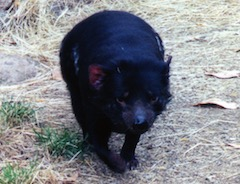
\includegraphics[width=\marginparwidth]{EigGen/TasmanianDevil}
\footnotesize\url{https://en.wikipedia.org/wiki/Tasmanian_devil}}
derive a mathematical model in the form \(\yv(t+1)=A\yv(t)\) for the age structure of the Tasmanian Devil.
By finding eigenvalues and an eigenvector, predict the long-term growth of the population, and predict the long-term relative numbers of Devils of various ages.
\begin{quoted}{Wikipedia, 2016}
Devils are not monogamous, and their reproductive process is very robust and competitive. Males fight one another for the females, and then guard their partners to prevent female infidelity. Females can ovulate three times in as many weeks during the mating season, and 80\%~of two-year-old females are seen to be pregnant during the annual mating season. Females average four breeding seasons in their life and give birth to 20--30 live young after three weeks' gestation. The newborn are pink, lack fur, have indistinct facial features and weigh around 0.20\,g (0.0071\,oz) at birth. As there are only four nipples in the pouch, competition is fierce and few newborns survive. The young grow rapidly and are ejected from the pouch after around 100~days, weighing roughly 200\,g (7.1\,oz). The young become independent after around nine months, so the female spends most of her year in activities related to birth and rearing.
\end{quoted}
\end{exercise}






\begin{exercise} \label{ex:} 
From the following partial description of the \idx{elephant}, 
\marginpar{\includegraphics[width=\marginparwidth]{EigGen/Loxodontacyclotis}
\footnotesize\url{https://en.wikipedia.org/wiki/Elephant}}
derive a mathematical model in the form \(\yv(t+1)=A\yv(t)\) for the age structure of the \idx{elephant}.
By finding eigenvalues and an eigenvector, predict the long-term growth of the population, and predict the long-term relative numbers of elephants of various ages.
\begin{quoted}{Wikipedia, 2016}
Gestation in elephants typically lasts around two years with interbirth intervals usually lasting four to five years. Births tend to take place during the wet season. Calves are born 85\,cm (33\,in) tall and weigh around 120\,kg (260\,lb). Typically, only a single young is born, but twins sometimes occur.  The relatively long pregnancy is maintained by five corpus luteums (as opposed to one in most mammals) and gives the foetus more time to develop, particularly the brain and trunk. As such, newborn elephants are precocial and quickly stand and walk to follow their mother and family herd.  A new calf is usually the centre of attention for herd members.  Adults and most of the other young will gather around the newborn, touching and caressing it with their trunks.  For the first few days, the mother is intolerant of other herd members near her young.  Alloparenting---where a calf is cared for by someone other than its mother---takes place in some family groups.  Allomothers are typically two to twelve years old. When a predator is near, the family group gathers together with the calves in the centre.

For the first few days, the newborn is unsteady on its feet, and needs the support of its mother. It relies on touch, smell and hearing, as its eyesight is poor. It has little precise control over its trunk, which wiggles around and may cause it to trip. By its second week of life, the calf can walk more firmly and has more control over its trunk. After its first month, a calf can pick up, hold and put objects in its mouth, but cannot suck water through the trunk and must drink directly through the mouth. It is still dependent on its mother and keeps close to her.

For its first three months, a calf relies entirely on milk from its mother for nutrition after which it begins to forage for vegetation and can use its trunk to collect water.  At the same time, improvements in lip and leg coordination occur.  Calves continue to suckle at the same rate as before until their sixth month, after which they become more independent when feeding.  By nine months, mouth, trunk and foot coordination is perfected.  After a year, a calf's abilities to groom, drink, and feed itself are fully developed.  It still needs its mother for nutrition and protection from predators for at least another year.  Suckling bouts tend to last 2--4\,min/hr for a calf younger than a year and it continues to suckle until it reaches three years of age or older.  Suckling after two years may serve to maintain growth rate, body condition and reproductive ability.  Play behaviour in calves differs between the sexes; females run or chase each other, while males play-fight. The former are sexually mature by the age of nine years while the latter become mature around 14--15 years.  Adulthood starts at about 18~years of age in both sexes.  Elephants have long lifespans, reaching 60--70~years of age.
\end{quoted}
\end{exercise}






\begin{exercise} \label{ex:} 
From the following partial description of the \idx{giant mouse lemur}, 
\marginpar{\includegraphics[width=\marginparwidth]{EigGen/Mirza_zaza}
\footnotesize\url{https://en.wikipedia.org/wiki/Giant_mouse_lemur}}
derive a mathematical model in the form \(\yv(t+1)=A\yv(t)\) for the age structure of the \idx{giant mouse lemur}.
By finding eigenvalues and an eigenvector, predict the long-term growth of the population, and predict the long-term relative numbers of \idx{giant mouse lemur}s of various ages.
\begin{quoted}{Wikipedia, 2016}
Reproduction starts in November for Coquerel's giant mouse lemur at Kirindy Forest; the estrous cycle runs approximately 22~days, while estrus lasts only a day or less. \ldots

One to three offspring (typically two) are born after 90~days of gestation, weighing approximately 12\,g (0.42\,oz). Because they are poorly developed, they initially remain in their mother's nest for up to three weeks, being transported by mouth between nests. Once they have grown sufficiently, typically after three weeks, the mother will park her offspring in vegetation while she forages nearby. After a month, the young begin to participate in social play and grooming with their mother, and between the first and second month, young males begin to exhibit early sexual behaviors (including mounting, neck biting, and pelvic thrusting). By the third month, the young forage independently, though they maintain vocal contact with their mother and use a small part of her range.

Females start reproducing after ten months, while males develop functional testicles by their second mating season. Testicle size in the northern giant mouse lemur does not appear to fluctuate by season, and is so large relative to the animal's body mass that it is the highest among all primates. This emphasis on sperm production in males, as well as the use of copulatory plugs, suggests a mating system best described as polygynandrous where males use scramble competition (roaming widely to find many females). In contrast, male Coquerel's giant mouse lemurs appear to fight for access to females (contest competition) during their breeding season. Males disperse from their natal range, and the age at which they leave varies from two years to several. Females reproduce every year, although postpartum estrus has been observed in captivity. In the wild, the lifespan of giant mouse lemurs is thought to rarely exceed five or six years
\end{quoted}
\end{exercise}




\begin{exercise} \label{ex:} 
From the following partial description of the \idx{dolphin} (Indo-Pacific bottlenose dolphin), 
\marginpar{\includegraphics[width=\marginparwidth]{EigGen/Tursiops_aduncus}
\footnotesize\url{https://en.wikipedia.org/wiki/Indo-Pacific_bottlenose_dolphin}}
derive a mathematical model in the form \(\yv(t+1)=A\yv(t)\) for the age structure of the \idx{dolphin}.
(Assume only one calf is born at a time.)
By finding eigenvalues and an eigenvector, predict the long-term growth of the population, and predict the long-term relative numbers of \idx{dolphin}s of various ages.
\begin{quoted}{Wikipedia, 2016}
Indo-Pacific bottlenose dolphins live in groups that can number in the hundreds, but groups of five to 15 dolphins are most common.  In some parts of their range, they associate with the common bottlenose dolphin and other dolphin species, such as the humpback dolphin.

The peak mating and calving seasons are in the spring and summer, although mating and calving occur throughout the year in some regions. Gestation period is about 12~months. Calves are between 0.84 and 1.5~metres (2.8 and 4.9\,ft) long, and weigh between 9 and 21~kilograms (20 and 46\,lb). The calves are weaned between 1.5 and two years, but can remain with their mothers for up to five years. The interbirth interval for females is typically four to six years.

In some parts of its range, this dolphin is subject to predation by sharks; its life span is more than 40 years.
\end{quoted}
\end{exercise}






\begin{exercise} \label{ex:} 
You are given that a mathematical model of the age structure of some animal population is
\begin{eqnarray*}
y_1(t+1)&=& 0.5y_1(t)+y_3(t),\\
y_2(t+1)&=& 0.5y_1(t)+0.7y_2(t),\\
y_3(t+1)&=& 0.3y_2(t)+0.9y_3(t).
\end{eqnarray*}
Invent an animal species, and time scale, and create details of a plausible scenario for the breeding and life cycle of the species that could lead to this mathematical model.  
Write a coherent paragraph about the breeding and life cycle of the species with enough information that someone could deduce this mathematical model from your description.  
Be creative.
\end{exercise}











\begin{exercise} \label{ex:} 
For each of the following matrices, say~\(A\) for instance, find by hand calculation the \idx{eigenvalue}s and \idx{eigenvector}s of the larger matrix~\(\begin{bmatrix} O&A\\\tr A&O \end{bmatrix}\).
Show your working.
Relate these to an \svd\ of the matrix~\(A\).
\begin{parts}
\item \(\eAii=\begin{bmatrix} 3\\4 \end{bmatrix}\)
\answer{\(\lambda=0,\pm5\), \((\frac45,-\frac35,0)\) and \((\frac35,\frac45,\pm1)\)}

\item \(\eAii=\begin{bmatrix} -5&12 \end{bmatrix}\)
\answer{\(\lambda=0,\pm13\), \((0,\frac{12}{13},\frac5{13})\) and \((\pm1,-\frac5{13},\frac{12}{13})\)}

\item \(\eAii=\begin{bmatrix} 1&0\\0&-2 \end{bmatrix}\)
\answer{\(\lambda=\pm1,\pm2\), \((\pm1,0,1,0)\) and \((0,1,0,\mp1)\)}

\item \(\eAii=\begin{bmatrix} 0&1\\-4&0 \end{bmatrix}\)
\answer{\(\lambda=\pm1,\pm4\), \((1,0,0,\pm1)\) and \((0,1,\mp1,0)\)}

\end{parts}
\end{exercise}




\begin{exercise} \label{ex:} 
Find by hand calculation all eigenvalues and corresponding eigenvectors of the \idx{generalised eigen-problem} \(A\vv=\lambda B\vv\) for the following pairs of matrices.
Check your calculations with \script.
%\begin{verbatim}
%n=2,A=0+round(randn(n)*2),B=0+round(randn(n)*2),[v,d]=eig(A,B), v*diag(1./v(1,:))
%\end{verbatim}
\begin{enumerate}
\item \(A=\begin{bmatrix} 1 & 3
\\ 0 & 0 \end{bmatrix}\),
\(B=\begin{bmatrix} 0 & 3
\\ 4 & 4 \end{bmatrix}\)
\answer{eigenvalues \(0,\tfrac23\); eigenvectors proportional to \((3,-1),(1,-1)\), respectively}

\item \(A=\begin{bmatrix} -1 & 0
\\ 5 & 1 \end{bmatrix}\),
\(B=\begin{bmatrix} 1 & 2
\\ -1 & -2 \end{bmatrix}\)
\answer{eigenvalue \(\tfrac17\); eigenvectors proportional to \((1,-4)\)}

\item \(A=\begin{bmatrix} 3 & -1
\\ -1 & -2 \end{bmatrix}\),
\(B=\begin{bmatrix} -3 & -3
\\ 1 & -1 \end{bmatrix}\)
\answer{eigenvalues \(-1,\tfrac76\); eigenvectors proportional to \((1,0),(1,-\tfrac{13}6\), respectively}

\item \(A=\begin{bmatrix} 1 & -1
\\ 1 & -4 \end{bmatrix}\),
\(B=\begin{bmatrix} 1 & -0
\\ 2 & -2 \end{bmatrix}\)
\answer{eigenvalues \(1\pm \i/\sqrt2\), eigenvectors proportional to \((1,\mp \i/\sqrt2)\), respectively}

\item \(A=\begin{bmatrix} 0 & 1 & -2
\\ -2 & -1 & -2
\\ 1 & 0 & 2 \end{bmatrix}\),
\(B=\begin{bmatrix} 1 & 0 & 1
\\ 0 & -2 & 1
\\ -1 & -3 & -1 \end{bmatrix}\)
\answer{eigenvalues \(\tfrac73,-2,0\); eigenvectors proportional to \((1,-\tfrac18,-\tfrac{59}{104}),(0,0,1),(1,-1,-\tfrac12)\), respectively}

\item \(A=\begin{bmatrix} 0 & -2 & 1
\\ -4 & 2 & 3
\\ 2 & -2 & -1 \end{bmatrix}\),
\(B=\begin{bmatrix} 0 & 0 & -1
\\ 0 & 0 & -1
\\ -2 & 0 & 0 \end{bmatrix}\)
\answer{eigenvalues \(0,-2\); eigenvectors proportional to \((1,\tfrac12,1),(0,-\tfrac12,1)\), respectively}

\item \(A=\begin{bmatrix} -1 & 1 & -2
\\ -4 & 0 & 3
\\ 0 & -3 & 0 \end{bmatrix}\),
\(B=\begin{bmatrix} -1 & 1 & 1
\\ 5 & -2 & 1
\\ 2 & -2 & -2 \end{bmatrix}\)
\answer{eigenvalue \(-\tfrac{11}2\); eigenvectors proportional to \((15,22,-13)\)}

\item \(A=\begin{bmatrix} -1 & 2 & -1
\\ 0 & -2 & -1
\\ 3 & 2 & 1 \end{bmatrix}\),
\(B=\begin{bmatrix} -1 & 2 & -1
\\ 0 & 2 & 1
\\ 3 & 1 & -2 \end{bmatrix}\)
\answer{eigenvalues \(1,\tfrac{12}{17},-1\); eigenvectors proportional to \((1,0,0),(4,1,-2),(1,-7,-15)\), respectively}

\end{enumerate}
\end{exercise}


%\begin{verbatim}
%n=4,A=0+round(randn(n)*2),B=0+round(randn(n)),[v,d]=eig(A,B), diag(d)'
%\end{verbatim}
\begin{exercise} \label{ex:} 
Use \script\ to find and describe all eigenvalues and corresponding eigenvectors of the \idx{generalised eigen-problem} \(A\vv=\lambda B\vv\) for the following pairs of matrices.
\begin{enumerate}
\item \(A=\begin{bmatrix} -2 & 1 & -2 & -2
\\ -2 & 2 & -1 & 0
\\ -1 & 1 & 2 & 1
\\ 1 & -2 & -1 & -1 \end{bmatrix}\),
\(B=\begin{bmatrix} -1 & 0 & -3 & 1
\\ -1 & 1 & -1 & 1
\\ -1 & 1 & 0 & 1
\\ 3 & 5 & 0 & -2 \end{bmatrix}\)
\answer{eigenvalues \(21.72, 1.50, -0.08, -2.15\) \twodp}

\item \(A=\begin{bmatrix} 3 & 1 & -2 & -4
\\ -2 & -3 & -3 & 2
\\ 1 & 1 & 1 & 2
\\ 1 & 2 & 0 & 0 \end{bmatrix}\),
\(B=\begin{bmatrix} -2 & 1 & 1 & 1
\\ 1 & -1 & 1 & -1
\\ 2 & 0 & -1 & 0
\\ 0 & 0 & 1 & 0 \end{bmatrix}\)
\answer{eigenvalues \(-5.26, 1.53, -0.98\) \twodp}

\item \(A=\begin{bmatrix} 0 & 2 & -1 & -1
\\ 0 & 0 & -1 & 0
\\ 3 & -3 & -1 & 1
\\ 2 & -3 & -2 & -3 \end{bmatrix}\),
\(B=\begin{bmatrix} 1 & 2 & 1 & 1
\\ 1 & 0 & 0 & -1
\\ 0 & 0 & 0 & 0
\\ 2 & -1 & -1 & 0 \end{bmatrix}\)
\answer{eigenvalues \(0.73\pm1.13\i, -1.37\) \twodp}

\item \(A=\begin{bmatrix} 4 & 4 & 0 & 3
\\ 1 & -2 & 0 & 1
\\ 0 & 2 & 4 & 2
\\ 0 & 2 & -1 & 1 \end{bmatrix}\),
\(B=\begin{bmatrix} -1 & 2 & -1 & 1
\\ -2 & 2 & 1 & 1
\\ -1 & 0 & 1 & -2
\\ 1 & 1 & 1 & -1 \end{bmatrix}\)
\answer{eigenvalues \(2.74, -2.20, -0.50\pm0.62\i\) \twodp}
  
\end{enumerate}
\end{exercise}


\begin{exercise} \label{ex:} 
Use the properties of determinants (\autoref{ch:ddm}), and that an \(n\)th~degree polynomial has exactly \(n\)~zeros (when counted according to multiplicity), to explain why the generalised eigen-problem \(A\vv=\lambda B\vv\), for real \(n\times n\) matrices~\(A\) and~\(B\), has \(n\)~eigenvalues iff matrix~\(B\) is invertible.
\end{exercise}


%\begin{verbatim}
%n=2,A=randn(2);A=0+round(A+A'),B=randn(n);B=0+round(B+B'),[v,d]=eig(A,B)
%\end{verbatim}
\begin{exercise} \label{ex:} 
Consider the \idx{generalised eigen-problem} \(A\vv=\lambda B\vv\) and let \(\lambda_1\neq\lambda_2\) be distinct eigenvalues with corresponding eigenvectors~\(\vv_1\) and~\(\vv_2\), respectively.
Invent two real \emph{symmetric} matrices~\(A\) and~\(B\) and record your working which demonstrates that although~\(\vv_1\) and~\(\vv_2\) are not orthogonal, nonetheless \(\tr{\vv_1}B\vv_2=0\).
\answer{one possibility is \(A=\begin{bmatrix} -1&-1\\-1&1 \end{bmatrix}\) and \(B=\begin{bmatrix} 1&1\\1&0 \end{bmatrix}\)} 
\end{exercise}


\begin{exercise} \label{ex:eennmov} 
Consider the \idx{generalised eigen-problem} \(A\vv=\lambda B\vv\) for real \emph{symmetric} \(n\times n\) matrices~\(A\) and~\(B\). 
Let \(\lambda_1\neq\lambda_2\) be distinct eigenvalues with corresponding eigenvectors~\(\vv_1\) and~\(\vv_2\), respectively.
Prove that \(\tr{\vv_1}B\vv_2=0\) always holds.
\end{exercise}


\begin{exercise} \label{ex:eennmre} 
Prove that if both~\(A\) and~\(B\) are real \emph{symmetric} \(n\times n\) matrices, then the eigenvalues of the \idx{generalised eigen-problem} \(A\vv=\lambda B\vv\) are all real.
Briefly explain why it is necessary to also have the additional proviso that the eigenvalues of~\(B\) are either all positive or all negative.
\end{exercise}


\begin{exercise} \label{ex:} 
In view of the preceding \autoref{ex:eennmre},
invent real symmetric matrices~\(A\) and~\(B\) such that the generalised eigen-problem \(A\vv=\lambda B\vv\) has complex valued eigenvalues.
% A=[0 1;1 0], B=[1 0;0 -1] will suffice, or vice versa.
\end{exercise}



\begin{exercise} \label{ex:} 
Explain briefly how the properties established in the the previous two Exercises~\ref{ex:eennmov} and~\ref{ex:eennmre} generalise important properties of the standard eigen-problem \(A\xv=\lambda\xv\) for symmetric~\(A\).
\end{exercise}






%\begin{verbatim}
%n=3,dt=0.5
%rs=[1 1/2 1/3 2/3 3/2 1/4 3/4 4/3]
%erat=rs(randperm(length(rs),n))
%[cn,cd]=rat(randn(1,n),0.2);
%[r,t]=meshgrid(erat,(0:2*n-1)*dt);
%f=(r.^t)*(cn./cd)'
%A=hankel(f(2:n+1),f(n+1:2*n))
%B=hankel(f(1:n),f(n:2*n-1))
%lambda=eig(A,B)
%r=log(lambda)/dt
%[U,P]=meshgrid(lambda,0:n-1);
%U=U.^P
%rcond(U)
%c=U\f(1:n)
%expr=exp(r)
%\end{verbatim}
\begin{exercise} \label{eg:}
Consider the specified data values~\fv\ at the specified times, and by hand or \script\ fit a sum of exponentials~\eqref{eq:eiddse}, \(f(t)=c_1e^{r_1t}+c_2e^{r_2t}+\cdots+c_ne^{r_nt}\).
Plot the data and the curve you have fitted.
\begin{enumerate}
\item For times \(0,1,2,3\) the data values are \[\fv=(3, 2.75, 2.5625, 2.4219).\]
\answer{\(f=(3/4)^t+2\)}

\item For times \(0,1,2,3\) the data values are \[\fv=(1.5833, 1.3333, 1.3056, 1.4954).\]
\answer{\(f=\tfrac54(2/3)^t+\tfrac13(3/2)^t\)}

\item For times \(0,2,4,6\) the data values are \[\fv=(-1, 0.222222, 0.172840, 0.085048).\]
\answer{\(f=-2(1/3)^t+(2/3)^t\)}

\item For times \(0,0.5,1,1.5\) the data values are \[\fv=(1.3, 0.75355, 0.45, 0.27678).\]
\answer{\(f=\tfrac45(1/4)^t+\tfrac12(1/2)^t\)}

\item For times \(0,1,2,\ldots,5\) the data values are 
\setbox\ajrqrbox\hbox{\qrcode{% f
f=[-1.00000
  0.12500
  0.71875
  1.03906
  1.21680
  1.31885]
}}\marginpar{\usebox{\ajrqrbox}}%
\[ \fv=\begin{bmatrix} -1.00000
\\ 0.12500
\\ 0.71875
\\ 1.03906
\\ 1.21680
\\ 1.31885 \end{bmatrix}.\]
\answer{\(f=-2(1/2)^t-\tfrac12(3/4)^t+\tfrac32\)}
  
\item For times \(0,1,2,\ldots,5\) the data values are 
\setbox\ajrqrbox\hbox{\qrcode{% f
f=[3.250000
   2.041667
   1.225694
   0.673900
   0.300178
   0.046636]
}}\marginpar{\usebox{\ajrqrbox}}%
\[ \fv=\begin{bmatrix} 3.250000
\\ 2.041667
\\ 1.225694
\\ 0.673900
\\ 0.300178
\\ 0.046636 \end{bmatrix}.\]
\answer{\(f=3.25(2/3)^t+\tfrac12(3/4)^t-\tfrac12\)}
  
\item For times \(0,2,4,\ldots,10\) the data values are 
\setbox\ajrqrbox\hbox{\qrcode{% f
f=[0.16667
    1.38889
    2.72984
    5.81259
   12.88104
   28.87004]
}}\marginpar{\usebox{\ajrqrbox}}%
\[ \fv=\begin{bmatrix} 0.16667
\\ 1.38889
\\ 2.72984
\\ 5.81259
\\ 12.88104
\\ 28.87004 \end{bmatrix}.\]
\answer{\(f=\tfrac12(3/2)^t-(1/3)^t+\tfrac23(3/4)^t\)}
  
\item For times \(0,0.5,1,\ldots,2.5\) the data values are 
\setbox\ajrqrbox\hbox{\qrcode{% f
f=[0.75000
  0.89846
  1.08333
  1.30323
  1.55903
  1.85343]
}}\marginpar{\usebox{\ajrqrbox}}%
\[ \fv=\begin{bmatrix} 0.75000
\\ 0.89846
\\ 1.08333
\\ 1.30323
\\ 1.55903
\\ 1.85343 \end{bmatrix}.\]
\answer{\(f=(4/3)^t+\tfrac14(1/2)^t-\tfrac12(3/4)^t\)}
  
\end{enumerate}
\end{exercise}



%\begin{verbatim}
%n=4,dt=2
%ws=1+rand(1,n/2),rs=-rand(1,n/2)
%ps=pi*rand(1,n/2),cs=randn(1,n/2)
%ts=(0:2*n-1)'*dt;
%f=0;for k=1:n/2,f=f+cs(k)*exp(rs(k)*ts).*cos(ws(k)*ts+ps(k));end
%f=f
%A=hankel(f(2:n+1),f(n+1:2*n));
%B=hankel(f(1:n),f(n:2*n-1));
%lambda=eig(A,B)
%r=log(lambda)/dt
%U=bsxfun(@power,lambda,0:n-1).';
%rcond(U)
%c=U\f(1:n);
%expr=exp(r);
%\end{verbatim}
\begin{exercise} \label{ex:} 
Consider the specified data values~\fv\ of some decaying oscillations at the specified times (in seconds).
Use \script\ to fit a sum of exponentials~\eqref{eq:eiddse}, \(f(t)=c_1e^{r_1t}+c_2e^{r_2t}+\cdots+c_ne^{r_nt}\).
Confirm your fit reproduces the data values.
What frequencies do you detect in the fitted constants?
\begin{enumerate}
\item  For times \(0,1,2,\ldots,7\) the data values are 
\setbox\ajrqrbox\hbox{\qrcode{% f
f=[-0.153161
   0.484787
  -0.124780
  -0.283690
   0.201896
   0.174832
  -0.200418
  -0.092107]
}}\marginpar{\usebox{\ajrqrbox}}%
\[ \fv=\begin{bmatrix} -0.153161
\\  0.484787
\\ -0.124780
\\ -0.283690
\\  0.201896
\\  0.174832
\\ -0.200418
\\ -0.092107 \end{bmatrix}.\]
\answer{frequencies \(1.20\) and \(1.70\) radians/sec \twodp}
  
\item  For times \(0,1,2,\ldots,7\) the data values are 
\setbox\ajrqrbox\hbox{\qrcode{% f
f=[1.225432
   0.499044
   0.034164
  -0.093971
  -0.103784
  -0.028558
   0.033825
   0.026439]
}}\marginpar{\usebox{\ajrqrbox}}%
\[ \fv=\begin{bmatrix} 1.225432
\\  0.499044
\\  0.034164
\\ -0.093971
\\ -0.103784
\\ -0.028558
\\  0.033825
\\  0.026439 \end{bmatrix}.\]
\answer{frequencies \(1.57\) and \(1.16\) radians/sec \twodp}
  
\item  For times \(0,0.5,1,\ldots,3.5\) the data values are 
\setbox\ajrqrbox\hbox{\qrcode{% f
f=[0.0060901
   0.1753701
   0.2385516
   0.1787653
   0.0404368
  -0.0998597
  -0.1742818
  -0.1552607]
}}\marginpar{\usebox{\ajrqrbox}}%
\[ \fv=\begin{bmatrix} 0.0060901
\\  0.1753701
\\  0.2385516
\\  0.1787653
\\  0.0404368
\\ -0.0998597
\\ -0.1742818
\\ -0.1552607 \end{bmatrix}.\]
\answer{frequencies \(1.94\) and \(1.46\) radians/sec \twodp}
  
\item  For times \(0,2,4,\ldots,14\) the data values are 
\setbox\ajrqrbox\hbox{\qrcode{% f
f=[1.297867
  -0.800035
   0.487305
  -0.285714
   0.161499
  -0.090411
   0.051244
  -0.028936]
}}\marginpar{\usebox{\ajrqrbox}}%
\[ \fv=\begin{bmatrix} 1.297867
\\ -0.800035
\\  0.487305
\\ -0.285714
\\  0.161499
\\ -0.090411
\\  0.051244
\\ -0.028936 \end{bmatrix}.\]
\answer{frequencies \(1.01\) and \(1.53\) radians/sec \twodp}
  
\end{enumerate}
\end{exercise}




% supernova CN1991T perhaps \cite[p.146, Ch.~8]{Pereyra2010}
% days from 2448300 and 20-B, digitised from SN1991T.pdf
%   64.2857    7.2833
%   65.0794    7.5333
%   66.6667    7.8500
%   73.8095    8.2500
%   81.7460    8.1333
%   88.0952    7.6000
%   95.2381    6.8667
%  104.7619    5.9167
%  121.4286    5.4500
%  132.5397    5.2500
%  146.0317    5.0333
%  159.5238    4.8667
% use data 3 to 8, say roughly 8 days apart, and mangle to get real
%\begin{verbatim}
%n=3,dt=8
%f=[0.6543
%   1.5783
%   1.6406
%   0.3678
%   0.05918
%   0.008227]
%A=hankel(f(2:n+1),f(n+1:2*n));
%B=hankel(f(1:n),f(n:2*n-1));
%lambda=eig(A,B)
%r=log(lambda)/dt
%U=bsxfun(@power,lambda,0:n-1).';
%rcond(U)
%c=U\f(1:n)
%\end{verbatim}
\begin{exercise} \label{ex:} 
In astronomy, Type~Ia supernova explode, peaking in luminosity in a few days, and then their luminosity declines over months. 
It is conjectured that the decline is powered by the radioactive decay from radioactive Nickel to Cobalt to Iron.
For the supernova \textsc{sn1991t} six measurements, starting on Julian day 2448366 and taken approximately 8~days apart, give the following luminosity values (in some units) \cite[p.146]{Pereyra2010}:
\setbox\ajrqrbox\hbox{\qrcode{% lumen
f=[0.6543
   1.5783
   1.6406
   0.3678
   0.05918
   0.008227]
}}\marginpar{\usebox{\ajrqrbox}}%
\begin{equation*}
\fv=\begin{bmatrix} 0.6543
\\ 1.5783
\\ 1.6406
\\ 0.3678
\\ 0.05918
\\ 0.008227 \end{bmatrix}
\end{equation*}
Detect the exponential decay in this supernova data by fitting a sum of exponentials~\eqref{eq:eiddse}, \(f(t)=c_1e^{r_1t}+c_2e^{r_2t}+c_3e^{r_3t}\).
Comment on the result.
\answer{\(f=1459e^{-0.36t}-2044e^{-0.33t}+585e^{-0.27t}\) where \(t\) is days post-2448366; but rcond is very poor!}
\end{exercise}




%\begin{verbatim}
%year=(1944:1993)';
%soi=[-0.03; 0.74; 6.37; -7.28; 0.44; -0.99; 1.32
%6.42; -6.51; 0.07; -1.96; 1.72; 6.49; -5.61
%-0.24; -2.90; 1.92; 6.54; -4.61; -0.47; -3.82
%1.94; 6.56; -3.53; -0.59; -4.69; 1.76; 6.53
%-2.38; -0.59; -5.48; 1.41; 6.41; -1.18; -0.45
%-6.19; 0.89; 6.19; 0.03; -0.16; -6.78; 0.21; 5.84
%1.23; 0.30; -7.22; -0.60; 5.33; 2.36; 0.91 ];
%n=length(year)/2, dt=1
%A=hankel(soi(2:n+1),soi(n+1:2*n));
%B=hankel(soi(1:n),soi(n:2*n-1));
%lambda=eig(A,B)
%r=log(lambda)/dt
%U=bsxfun(@power,lambda,0:n-1).';
%rcond(U)
%c=U\soi(1:n)
%expr=exp(r);
%\end{verbatim}
\begin{exercise} \label{ex:} 
Recall that \autoref{eg:orthbapp} introduced the phenomenon of \idx{El Nino} which makes a large impact on the world's weather.
El Nino is correlated significantly with the difference in atmospheric pressure between Darwin and Tahiti---the so-called \idx{Southern Oscillation Index} (\soi).
\autoref{fig:soiRoundData} plots a (`smoothed') yearly average \soi\ each year for fifty years up to 1993.
Here detect the cycles in the \soi\ by analysing the plotted data as a sum of exponentials~\eqref{eq:eiddse}, \(f(t)=c_1e^{r_1t}+c_2e^{r_2t}+\cdots+c_ne^{r_nt}\).
\begin{enumerate}
\item Enter the data into \script:
\setbox\ajrqrbox\hbox{\qrcode{% soi
year=(1944:1993)';
soi=[-0.03; 0.74; 6.37; -7.28; 0.44; -0.99; 1.32
6.42; -6.51; 0.07; -1.96; 1.72; 6.49; -5.61
-0.24; -2.90; 1.92; 6.54; -4.61; -0.47; -3.82
1.94; 6.56; -3.53; -0.59; -4.69; 1.76; 6.53
-2.38; -0.59; -5.48; 1.41; 6.41; -1.18; -0.45
-6.19; 0.89; 6.19; 0.03; -0.16; -6.78; 0.21; 5.84
1.23; 0.30; -7.22; -0.60; 5.33; 2.36; 0.91 ];
}}\marginpar{\usebox{\ajrqrbox}}%
\begin{verbatim}
year=(1944:1993)';
soi=[-0.03; 0.74; 6.37; -7.28; 0.44; -0.99; 1.32
6.42; -6.51; 0.07; -1.96; 1.72; 6.49; -5.61
-0.24; -2.90; 1.92; 6.54; -4.61; -0.47; -3.82
1.94; 6.56; -3.53; -0.59; -4.69; 1.76; 6.53
-2.38; -0.59; -5.48; 1.41; 6.41; -1.18; -0.45
-6.19; 0.89; 6.19; 0.03; -0.16; -6.78; 0.21; 5.84
1.23; 0.30; -7.22; -0.60; 5.33; 2.36; 0.91 ];
\end{verbatim}

\item Use \autoref{pro:ei} in \script\ to compute the twenty-five complex rates~\rv\ and twenty-five complex coefficients~\cv\ that fit the data.
% albeit poor rcond

\item Find the four relatively large coefficients, when compared to the relatively small coefficients of magnitude\({}<0.015\).
% should really look at size of c*exp(Re(r)t)---but almost the same

\item Explain why these four coefficients indicate that the \soi\ data appears to be dominantly composed of oscillations with periods about \(5.1\)~years and \(2.5\)~years.
% is the 2.5 year a harmonic of the 5 year oscillation?

\end{enumerate}
\end{exercise}











\begin{exercise} 
In a few sentences, answer\slash discuss each of the the following.
\begin{enumerate}
\item  Given an \(n\times n\) matrix, what leads to the characteristic polynomial being of \(n\)th~degree?

\item How does the trace of a matrix appear in its characteristic polynomial?

\item What is the importance of the multiplicity of eigenvalues of a matrix?

\item What is the relation between the characteristic polynomial of a matrix and its characteristic equation?

\item Why is it beautifully useful to cater for complex valued eigenvalues and eigenvectors of real matrices arising in real problems?

\item What is the evidence for repeated eigenvalues generally being sensitive to computational and experimental errors?

\item What causes \(\yv(t)=c_1\lambda_1^t\vv_1+c_2\lambda_2^t\vv_2+\cdots+c_m\lambda_m^t\vv_m\) to form a general solution to the evolving system \(\yv(t+1)=A\yv(t)\)?

\item How can the singular values of a matrix arise from an eigen-problem?

\item Describe some scenarios that require fitting a sum of exponentials to data.

\end{enumerate}
\end{exercise}

\begin{comment}%{ED498555.pdf}
why, what caused X?
how did X occur?
what-if? what-if-not?
how does X compare with Y?
what is the evidence for X?
why is X important?
\end{comment}





%!TEX root = ../larxxia.tex

\section{Linearly independent vectors may form a basis}
\label{sec:lisb}

\secttoc
\begin{comment}
\pooliv{p.92--7,198--208} \holti{\S2.3}
\end{comment}

\index{linearly dependent|(}
\index{linearly independent|(}
\index{linear dependence|(}
\index{linear independence|(}


In \cref{ch:eesm} on symmetric matrices, the \idx{eigenvector}s from \idx{distinct eigenvalues} are proved to be always \idx{orthogonal}---because of matrix symmetry.  
For general matrices, the eigenvectors are not orthogonal---as introduced at the start of this \cref{ch:gee}.  
But the orthogonal property is extremely useful.
Question: is there some analogue of orthogonality that is similarly useful for general matrices?
Answer: yes. 
We now extend ``orthogonal'' to the more general concept of \text{``linearly independent''.}

One reason that \idx{orthogonal vectors} are useful is that they can form an \idx{orthonormal basis} and hence act as the unit vectors of an orthogonal coordinate systems.
Analogously, the concept of linearly independent vectors is closely connected to \idx{coordinate system}s that are not orthogonal.



\paragraph{Subspace \idx{coordinate system}s} 
In any given mathematical problem, an application wants two things from a \idx{general solution}: 
\begin{itemize}
\item firstly, the general solution must encompass every possibility (the solution must span the possibilities); and 
\item secondly, each possible solution should have a unique algebraic form in the general solution.
\end{itemize}
For an example of the need for a unique algebraic form, let's suppose we wanted to find solutions to the \idx{differential equation} \(d^2y/dt^2-y=0\)\,. 
You might find \(y=3e^x+2e^{-x}\), whereas I find \(y=5\cosh x+\sinh x\), and a friend finds \(y=e^x+4\cosh x\).
It appears from these disparate algebraic forms that we all disagree.
Should we all go and search for errors in the solution process?  No.
The reason is that all these solutions are the same.
The apparent differences arise only because you choose \idx{exponential}s to represent the solution, whereas I choose hyperbolic functions, and the friend a mixture; the solutions are the same, it is only the algebraic representation that appears different. 
In general, when we cannot immediately distinguish identical solutions, all algebraic manipulation becomes immensely more difficult due to algebraic ambiguity.
To avoid such immense difficulties we need to introduce, in both calculus and linear algebra, the concept of \text{linear independence.}

\needlines6
\begin{wrapfigure}r{0pt}
\begin{tikzpicture}
\newcommand{\ppoint}[2]{
    \pgfmathparse{#1*3+#2*1}\let\h\pgfmathresult
    \pgfmathparse{#1*1+#2*2}\let\v\pgfmathresult
    \addplot[red,mark=*,only marks] coordinates {(\h,\v)};
    \edef\tempe{\noexpand
    \node[left] at (axis cs:\h,\v) {$(#1,#2)$};
    }\tempe
    }
\begin{axis}[footnotesize,font=\footnotesize
  ,axis lines=none%,xlabel={$x$},ylabel={$y$}
  , axis equal image
  , view={0}{90}
  ,xmax=7.5,ymax=5.5,xmin=-7.6,ymin=-5.6
  ]
\addplot3[mesh,brown,samples=17,domain=-4:4,dotted] (3*x+y,x+2*y,0);
\addplot3[mesh,brown,samples=9,domain=-4:4] (3*x+y,x+2*y,0);
\addplot[blue,quiver={u=3,v=1},-stealth,thick] coordinates {(0,0)};
\node[right] at (axis cs:3,1) {$\vv_1$};
\addplot[blue,quiver={u=1,v=2},-stealth,thick] coordinates {(0,0)};
\node[above] at (axis cs:1,2) {$\vv_2$};
\ppoint21
\ppoint1{-3}
\ppoint{-2}3
\ppoint00
\end{axis}
\end{tikzpicture}
\end{wrapfigure}
Linear independence empowers us, often implicitly, to use a non-orthogonal \idx{coordinate system} in a \idx{subspace}.
We replace orthogonal \idx{unit vector}s by any suitable set of basis vectors.
For example, in the plane any two vectors at an angle to each other suffice to be able to describe uniquely every vector (point) in the plane.
As illustrated to the right, every point in the plane (end-point of a vector) is a unique \idx{linear combination} of the two drawn basis vectors~\(\vv_1\) and~\(\vv_2\).
Such a pair of basis vectors, termed a linearly independent pair, avoids the  difficulties of \text{algebraic ambiguity.}



\subsection{Linearly (in)dependent sets}

This section defines ``linearly dependent'' and ``linearly independent'', and then relates the concept to homogeneous linear equations, orthogonality, and sets of eigenvectors.


\begingroup
\def\temp#1{\begin{tikzpicture}% following top aligns tikzpicture
[baseline={([yshift={-\ht\strutbox}]current bounding box.north)}]
\begin{axis}[footnotesize,font=\footnotesize
  ,axis lines=middle, axis equal image
  ,xmax=2.3,ymax=2.3
  ]
\addplot[blue,quiver={u=2,v=1},-stealth,thick] coordinates {(0,0)};
\node[below] at (axis cs:2,1) {$\vv_1$};
\addplot[blue,quiver={u=1,v=2},-stealth,thick] coordinates {(0,0)};
\node[below] at (axis cs:1,2) {$\quad\vv_2$};
\ifcase#1
\or%1
\addplot[brown,quiver={u=-1.333,v=-0.667},-stealth] coordinates {(0,0)};
\addplot[brown,quiver={u=1.333,v=2.667},-stealth] coordinates {(-1.333,-0.667)};
\addplot[red,quiver={u=0,v=2},-stealth,thick] coordinates {(0,0)};
\node[right] at (axis cs:0,2) {$(0,2)$};
\or%2
\addplot[brown,quiver={u=1.333,v=0.667},-stealth] coordinates {(0,0)};
\addplot[brown,quiver={u=0.667,v=1.333},-stealth] coordinates {(1.333,0.667)};
\addplot[red,quiver={u=2,v=2},-stealth,thick] coordinates {(0,0)};
\node[left] at (axis cs:2,2) {$(2,2)$};
\or%3
\addplot[brown,quiver={u=2,v=1},-stealth] coordinates {(0,0)};
\addplot[brown,quiver={u=-1,v=-2},-stealth] coordinates {(2,1)};
\addplot[red,quiver={u=1,v=-1},-stealth,thick] coordinates {(0,0)};
\node[above] at (axis cs:1,-1) {\quad\qquad$(1,-1)$};
\or%4
\addplot[brown,quiver={u=-2,v=-1},-stealth] coordinates {(0,0)};
\addplot[brown,quiver={u=-1,v=-2},-stealth] coordinates {(-2,-1)};
\addplot[red,quiver={u=-3,v=-3},-stealth,thick] coordinates {(0,0)};
\node[above] at (axis cs:-3,-3) {\qquad\qquad$(-3,-3)$};
\else
\fi
\end{axis}
\end{tikzpicture}}%
\needlines7
\begin{wrapfigure}r{0pt} \temp0 \end{wrapfigure}
\begin{example}[2D \idx{non-orthogonal coordinates}] \label{eg:2dnoc}
Show that every vector in the plane~\(\RR^2\) can be written uniquely as a \idx{linear combination} of the two vectors \(\vv_1=(2,1)\) and \(\vv_2=(1,2)\) that are shown to the right.
\vspace*{3\baselineskip} % lines to clear the graphic??

\begin{solution} 
Let's start with some specific example vectors.
\def\tmpp#1#2{\parbox[t]{20em}{\raggedright #2} \temp{#1}}
\begin{enumerate}
\item \tmpp1{The vector \((0,2)\) may be written as the linear combination \((0,2)=-\frac23\vv_1+\frac43\vv_2\) as shown.} 

\item \tmpp2{The vector \((2,2)\) may be written as the linear combination \((2,2)=\frac23\vv_1+\frac23\vv_2\) as shown.}

\item \tmpp3{The vector \((1,-1)\) may be written as the linear combination \((1,-1)=\vv_1-\vv_2\) as shown.}

\item \tmpp4{The vector \((-3,-3)\) may be written as the linear combination \((-3,-3)=-\vv_1-\vv_2\) as shown.}

\end{enumerate}

\begin{wrapfigure}r{0pt}
\begin{tikzpicture}
\begin{axis}[small,font=\footnotesize
  ,axis lines=middle, axis equal image, view={0}{90}
  ,xmax=5.5,ymax=5.5,xmin=-5.5,ymin=-5.5
  ,xlabel={$x$},ylabel={$y$}
  ]
\addplot3[mesh,brown,samples=13,domain=-3:3,dotted] (2*x+y,x+2*y,0);
\addplot3[mesh,brown,samples=7,domain=-3:3] (2*x+y,x+2*y,0);
\addplot[blue,quiver={u=2,v=1},-stealth,thick] coordinates {(0,0)};
\node[right] at (axis cs:2,1) {$\vv_1$};
\addplot[blue,quiver={u=1,v=2},-stealth,thick] coordinates {(0,0)};
\node[above] at (axis cs:1,2) {$\vv_2$};
\end{axis}
\end{tikzpicture}
\end{wrapfigure}
Now proceed to consider a general vector \((x,y)\) and seek it as a linear combination of~\(\vv_1\) and~\(\vv_2\), namely \((x,y)=c_1\vv_1+c_2\vv_2\)\,.
That is, let's write each and every point in the plane as a linear combination of~\(\vv_1\) and~\(\vv_2\) as illustrated to the right.
Rewrite the equation in matrix-vector form as
\begin{equation*}
\begin{bmatrix} \vv_1&\vv_2 \end{bmatrix}
\begin{bmatrix} c_1\\c_2 \end{bmatrix}
=\begin{bmatrix} x\\y \end{bmatrix}
,\quad\text{that is,}\quad
V\cv=\begin{bmatrix} x\\y \end{bmatrix}
\text{ for }V=\begin{bmatrix} 2&1\\1&2 \end{bmatrix}.
\end{equation*}
For any given \((x,y)\), \(V\cv=(x,y)\) is a system of linear equations for the coefficients~\cv.
\cref{thm:ftim2} asserts that the system has a unique solution~\cv\ if and only if the matrix~\(V\) is invertible.
Here the unique solution is then that the vector of coefficients
\begin{equation*}
\cv=V^{-1}\begin{bmatrix} x\\y \end{bmatrix}
=\begin{bmatrix} \frac23&-\frac13\\-\frac13&\frac23 \end{bmatrix}
\begin{bmatrix} x\\y \end{bmatrix}.
\end{equation*}
Equivalently, \cref{thm:ftim2iii} asserts the system has a unique solution~\cv---unique coefficients~\cv---if and only if the {homogeneous} system \(V\cv=\ov\) has only the zero solution \(\cv=\ov\)\,.
It is this last statement that leads to the upcoming \cref{def:lindep} of \idx{linearly independent} vectors.
\end{solution}
\end{example}
\endgroup



{%group
\def\temp{\begin{tikzpicture}
\begin{axis}[footnotesize,font=\footnotesize
  ,axis lines=middle, axis equal image
  ,xmax=2.3,ymax=2.3
  ]
\addplot[blue,quiver={u=2,v=1},-stealth,thick] coordinates {(0,0)};
\node[below] at (axis cs:2,1) {$\vv_1$};
\addplot[blue,quiver={u=1,v=2},-stealth,thick] coordinates {(0,0)};
\node[below] at (axis cs:1,2) {$\quad\vv_2$};
\addplot[red,quiver={u=-2.5,v=1},-stealth,thick] coordinates {(0,0)};
%\node[right] at (axis cs:-2.5,1) {$(-2.5,1)$};
\end{axis}
\end{tikzpicture}}
\begin{activity}[\temp]
The vector shown to the right is which of the following \idx{linear combination}s of shown vectors~\(\vv_1\) and~\(\vv_2\)?
\actposs{\(-2\vv_1 +1.5\vv_2\)}
{\(-2.5\vv_1 +2\vv_2\)}
{\(-1.5\vv_1 +\vv_2\)}
{\(-\vv_1 +\vv_2\)}
\end{activity}
}





\needlines8
\begin{wrapfigure}r{0pt}
\qview{113}{117}{\begin{tikzpicture}
\begin{axis}[small,font=\small
  ,xlabel={$x$}, ylabel={$y$}, zlabel={$z$},label shift={-2ex}
  ,no marks ,domain=-2.5:2.5,axis equal image,zmax=2.5,zmin=-2.5
  ,view={\q}{30}
  ] 
\addplot3[surf,blue,samples=3,opacity=0.3]  {-x-y};
\addplot3[blue,thick,quiver={u=-1,v=1,w=0},-stealth] coordinates {(0,0,0)};
\node[right] at (axis cs:-1,1,0) {$\vv_1$};
\addplot3[blue,thick,quiver={u=1,v=-2,w=1},-stealth] coordinates {(0,0,0)};
\node[below] at (axis cs:1,-2,1) {$\vv_2$};
\addplot3[blue,thick,quiver={u=0,v=1,w=-1},-stealth] coordinates {(0,0,0)};
\node[below] at (axis cs:0,1,-1) {$\vv_3$};
\end{axis}
\end{tikzpicture}}
\end{wrapfigure}
\begin{example}[3D failure] 
Show that vectors in~\(\RR^3\) are not written uniquely as a \idx{linear combination} of \(\vv_1=(-1,1,0)\), \(\vv_2=(1,-2,1)\), and \(\vv_3=(0,1,-1)\). 

One reason for the failure is that these three vectors only span a plane, as shown to the right in stereo.  
The solution here looks at the different issue of unique representation.

\begin{solution} 
As one example, consider the vector~\((1,0,-1)\):
\begin{eqnarray*}
(1,0,-1)&=&-1\vv_1+0\vv_2+1\vv_3\,;
\\(1,0,-1)&=&1\vv_1+2\vv_2+3\vv_3\,;
\\(1,0,-1)&=&-2\vv_1-1\vv_2+0\vv_3\,;
\\(1,0,-1)&=&(-1+t)\vv_1+t\vv_2+(1+t)\vv_3\,,\quad\text{for every }t.
\end{eqnarray*}
This last combination shows that there are an infinite number of ways to write \((1,0,-1)\) as a linear combination of~\(\vv_1\), \(\vv_2\), and~\(\vv_3\).
Such an infinity of linear combinations means that~\(\vv_1\), \(\vv_2\), and~\(\vv_3\) cannot form the basis for a useful `coordinate system' because we cannot easily distinguish between the different combinations all describing the same vector.
The reason for the infinity of combinations is that there is a nontrivial linear combination of~\(\vv_1\), \(\vv_2\), and~\(\vv_3\) which is zero, namely here \(\vv_1+\vv_2+\vv_3=\ov\)\,.
It is this last statement that leads to the \cref{def:lindep} of \text{\idx{linearly dependent} vectors.}
\end{solution}
\end{example}





\begin{definition} \label{def:lindep} 
A set of vectors \(\{\hlist\vv k\}\) is \bfidx{linearly dependent} if there are \idx{scalar}s \hlist ck, at least one of which is nonzero, such that \(\lincomb c\vv k=\ov\)\,.
A set of vectors that is not linearly dependent is called \bfidx{linearly independent} (characterized by \emph{only} the linear combination with \(c_1=c_2=\cdots=c_k=0\) gives the \text{\idx{zero vector}).}
\end{definition}

When reading the terms ``linearly in/dependent'' be very careful: it is all too easy to misread the presence or absence of the crucial ``in''~syllable. 
The presence or absence of the ``in''~syllable makes all the difference between the property and its opposite.


\begin{example} \label{eg:lindep}
Are the following sets of vectors linearly dependent or linearly independent.  Give reasons.
\begin{enumerate}[ref=\ref{eg:lindep}(\alph*)]
\item\label[example]{eg:lindepa} \(\{(-1,1,0),\ (1,-2,1),\ (0,1,-1)\}\) 
\begin{solution} 
The set is linearly dependent as the linear combination \((-1,1,0)+(1,-2,1)+(0,1,-1)=(0,0,0)\). 
\end{solution}

\item\label[example]{eg:lindepb} \(\{(2,1),\ (1,2)\}\) 
\begin{solution} 
The set is linearly independent because the linear combination equation \(c_1(2,1)+c_2(1,2)=(0,0)\) is equivalent to the homogeneous matrix-vector system \(\begin{bmat} 2&1\\1&2 \end{bmat}\cv=\ov\) which has \emph{only} the zero solution \(\cv=\ov\)\,. 
\end{solution}

%\item \(\{(-1,1,0),\ (1,-2,1)\}\)
%\begin{solution} 
%The set is linearly independent: for the linear combination \(c_1(-1,1,0)+c_2(1,-2,1)
%=(-c_1+c_2,c_1-2c_2,c_2)=\ov\) requires the last component to be zero which requires \(c_2=0\);
%then either of the other components requires \(c_1=0\)\,.
%\end{solution}

\item\label[example]{eg:lindepc} \(\{(-2,4,1,-1,0)\}\)
\begin{solution} 
This set of one vector in~\(\RR^5\) is linearly independent as \(c_1(-2,4,1,-1,0)=\ov\) can only be satisfied with \(c_1=0\)\,. 
Indeed, any one nonzero vector~\vv\ in~\(\RR^n\) forms a linearly independent set,~\(\{\vv\}\), for the same reason.
\end{solution}



\item \(\{(2,1),\ (0,0)\}\) 
\begin{solution} 
The set is linearly dependent because the linear combination  \(0(2,1)+c_2(0,0)=(0,0)\) for every nonzero~\(c_2\). 
\end{solution}


\item \(\{\ov,\hlist[2]\vv k\}\)
\begin{solution} 
Every  set that includes the zero vector is linearly dependent as
\(c_1\ov+0\vv_2+\cdots+0\vv_k=\ov\) for every nonzero~\(c_1\).
\end{solution}

\item \index{e@$\ev_j$}\(\{\ev_1,\ev_2,\ev_3\}\), the set of \idx{standard unit vector}s in~\(\RR^3\).
\begin{solution} 
This set is linearly independent as
\(c_1\ev_1+c_2\ev_2+c_3\ev_3=(c_1,c_2,c_3)=\ov\)
\emph{only} when all three components are zero, \(c_1=c_2=c_3=0\)\,. 
\end{solution}

\item \(\{(\frac13,\frac23,\frac23),\ (\frac23,\frac13,-\frac23)\}\)
\begin{solution} 
This set is linearly independent.
Seek some linear combination \(c_1(\frac13,\frac23,\frac23) +c_2(\frac23,\frac13,-\frac23) =\ov\)\,.
Take the dot product of both sides of this equation with \((1,2,2)\):
\begin{eqnarray*}
&&c_1\begin{bmatrix}\frac13\\\frac23\\\frac23 \end{bmatrix}\cdot\begin{bmatrix} 1\\2\\2 \end{bmatrix} +c_2\begin{bmatrix} \frac23\\\frac13\\-\frac23 \end{bmatrix}\cdot\begin{bmatrix} 1\\2\\2 \end{bmatrix} =\ov\cdot\begin{bmatrix} 1\\2\\2 \end{bmatrix}
\\\implies&& c_13+c_20=0
\implies c_1=0\,.
\end{eqnarray*}
Also, take the dot product with \((2,1,-2)\): 
\begin{eqnarray*}
&&c_1\begin{bmatrix}\frac13\\\frac23\\\frac23 \end{bmatrix}\cdot\begin{bmatrix} 2\\1\\-2 \end{bmatrix} +c_2\begin{bmatrix} \frac23\\\frac13\\-\frac23 \end{bmatrix}\cdot\begin{bmatrix} 2\\1\\-2 \end{bmatrix} =\ov\cdot\begin{bmatrix} 2\\1\\-2 \end{bmatrix}
\\\implies&& c_10+c_23=0
\implies c_2=0\,.
\end{eqnarray*}
Hence \(c_1=c_2=0\) is the \emph{only} possibility and so the two given vectors are linearly independent.
\end{solution}

\end{enumerate}
These last two cases generalize to the next \cref{thm:ortholi} about the linear independence of every \idx{orthonormal set} of vectors.
\end{example}



\begin{activity}
Which of the following sets of vectors is linearly independent?
\actposs{\(\{(-1,1),(0,1)\}\)}
{\(\{(0,0),(-2,1)\}\)}
{\(\{(0,1),(0,-1)\}\)}
{\(\{(-1,2),(-2,4)\}\)}
\end{activity}




\begin{example}[calculus extension] 
In calculus the notion of a function corresponds to the notion of a vector in our linear algebra.  
For the purposes of this example, consider `vector' and `function' to be synonymous, and that `all \idx{components}' and `all~\(x\)' are synonymous. 
Show that the set \(\{e^x,e^{-x},\cosh x,\sinh x\}\) is linearly dependent.  
What is a subset that is \text{linearly independent?}
\begin{solution} 
The definition of the hyperbolic functions, namely that \(\cosh x=(e^x+e^{-x})/2\) and \(\sinh x=(e^x-e^{-x})/2\), immediately gives two nontrivial linear combinations that are zero for all~\(x\), namely \(2\cosh x-e^x-e^{-x}=0\) and \(2\sinh x-e^x+e^{-x}=0\) for all~\(x\).
Either one of these implies that the set \(\{e^x,e^{-x},\cosh x,\sinh x\}\) is \text{linearly dependent.}

Because \(e^x\) and~\(e^{-x}\) are not proportional to each other, there is no linear combination which is zero for all~\(x\), and hence the set \(\{e^x,e^{-x}\}\) is linearly independent (as are any other pairs of the four functions).
\end{solution}
\end{example}







\begin{theorem} \label{thm:ortholi}
Every \idx{orthonormal set} of vectors (\cref{def:orthoset}) is \idx{linearly independent}.
\end{theorem}
\begin{proof} %Take dot products with the defining equation.
Let \(\{\hlist\vv k\}\) be an orthonormal set of vectors in~\(\RR^n\).
Let's find all possible scalars \hlist ck such that \(\lincomb c\vv k=\ov\)\,.
Taking the dot product of this equation with~\(\vv_1\) requires
\(c_1\vv_1\cdot\vv_1+c_2\vv_2\cdot\vv_1+\cdots+c_k\vv_k\cdot\vv_1=\ov\cdot\vv_1\)\,;
by orthonormality this equation becomes
\(c_11+c_20+\cdots+c_k0=0\)\,; that is, \(c_1=0\)\,.
Similarly, taking the dot product with~\(\vv_2\) requires
\(c_1\vv_1\cdot\vv_2+c_2\vv_2\cdot\vv_2+\cdots+c_k\vv_k\cdot\vv_2=\ov\cdot\vv_2\)\,;
by orthonormality this equation becomes
\(c_10+c_21+\cdots+c_k0=0\)\,; that is, \(c_2=0\)\,.
And so on for every vector in the set, implying the coefficients \(c_1=c_2=\cdots=c_k=0\) is the only possibility.
By \cref{def:lindep}, the orthonormal set must be \text{linearly independent.}
\end{proof}


In contrast to orthonormal vectors which are always linearly independent, a set of two vectors proportional to each other is always linearly dependent as seen in the following examples.
This linear dependence of proportional vectors then generalizes in the forthcoming \cref{thm:lindeplc}.




\begin{example} 
Show that the following sets are linearly dependent.
\begin{enumerate}
\item \(\{(1,2),\ (3,6)\}\)
\begin{solution} 
Since \((3,6)=3(1,2)\) then the linear combination \(1(3,6)-3(1,2)=\ov\) and the set is linearly dependent. 
\end{solution}

\item \(\{(2.2,-2.1,0,1.5),\ (-8.8,8.4,0,-6)\}\)
\begin{solution} 
Since  \((-8.8,8.4,0,-6)=-4(2.2,-2.1,0,1.5)\) then the linear combination 
\begin{equation*}
(-8.8,8.4,0,-6)+4(2.2,-2.1,0,1.5)=\ov\,,
\end{equation*}
and so the set is linearly dependent.
\end{solution}
\end{enumerate}
\end{example}




\begin{activity}
For what value of~\(c\) is the set \(\{(-3c,-2+2c),(1,2)\}\) linearly dependent?
%v=round(randn(2)*2)+0,w=round(randn(2))+0,0-eig(v,w)
\actposs[4]{\(c=\frac14\)}{\(c=-\frac13\)}{\(c=0\)}{\(c=1\)}
\end{activity}




\begin{theorem} \label{thm:lindeplc} 
A set of vectors \(\{\hlist\vv m\}\) is \idx{linearly dependent} if and only if at least one of the vectors can be expressed as a \idx{linear combination} of the other vectors.
In particular, a set of two vectors \(\{\vv_1,\vv_2\}\) is linearly dependent if and only if one of the vectors is a scalar multiple of \text{the other.}
\end{theorem}

\begin{proof} 
\cref{ex:lindeplc} establishes the particular case of a set of two vectors.
%Start with the particular case of the set of two vectors \(\{\vv_1,\vv_2\}\).
%Say \(\vv_1\) is a multiple of~\(\vv_2\), \(\vv_1=c\vv_2\)\,, then the linear combination \(\vv_1-c\vv_2=\ov\)\,, and so the set is linearly dependent. 
%Similarly if \(\vv_2\) is a multiple of~\(\vv_1\).
%Conversely, if the set is linearly dependent then \(c_1\vv_1+c_2\vv_2=0\) where one or both of \(c_1,c_2\neq0\): if \(c_1\neq 0\) then rearrange to \(\vv_1=-(c_2/c_1)\vv_2\) and so \(\vv_1\) is a multiple of~\(\vv_2\); and similarly if \(c_2\neq 0\)\,.

In the general case of \(m\)~vectors, first establish that if one of the vectors can be expressed as a {linear combination} of the others, then the set is linearly dependent.
Let's label the set of vectors so that it is vector~\(\vv_1\) which is a linear combination of the others; that is, \(\vv_1=\lincomb[2]c\vv m\)\,.
Rearranging, \((-1)\vv_1+\lincomb[2]c\vv m=\ov\)\,; that is, there is a non-trivial (as at least \(c_1=-1\neq0\)) linear combination of the set of vectors which is zero.
Hence the set is \text{linearly dependent.}

Second, establish the converse.  
Given the set is linearly dependent, there exist coefficients, not all zero, such that \(\lincomb c\vv m=\ov\)\,.  
Suppose that we have labelled the vectors so that \(c_1\neq 0\)\,.  
Then rearranging the equation gives
\(c_1\vv_1=-c_2\vv_2-c_3\vv_3-\cdots-c_m\vv_m\)\,.
Divide by the nonzero~\(c_1\) to deduce
\(\vv_1=-(c_2/c_1)\vv_2-(c_3/c_1)\vv_3-\cdots-(c_m/c_1)\vv_m\)\,;
that is, \(\vv_1\)~is a linear combination of the \text{other vectors.}
\end{proof}


\begin{example} 
Invoke \cref{thm:lindeplc} to deduce whether the following sets are linearly independent or linearly dependent.
\begin{enumerate}
\item \(\{(-1,1,0),\ (1,-2,1),\ (0,1,-1)\}\)
\begin{solution} 
Since \((1,-2,1)=-(-1,1,0)-(0,1,-1)\) the set must be linearly dependent.
\end{solution}

\item 
\begin{figbox}{\begin{tikzpicture}
\begin{axis}[footnotesize,font=\footnotesize
  ,axis lines=none, axis equal image
  ]
\addplot[blue,quiver={u=3,v=2},-stealth,thick] coordinates {(0,0)};
\node[below] at (axis cs:3,2) {$\vv_2$};
\addplot[blue,quiver={u=1,v=2},-stealth,thick] coordinates {(0,0)};
\node[right] at (axis cs:1,2) {$\vv_1$};
\addplot[black,mark=*] coordinates {(0,0)};
\end{axis}
\end{tikzpicture}}%
The set of two vectors shown to the right.

\begin{solution} 
Since the two vectors are not proportional to each other, we cannot write either as a scalar multiple of the other, and so the pair are linearly independent. 

\end{solution}
\end{figbox}


\item 
\begin{figbox}{\begin{tikzpicture}
\begin{axis}[footnotesize,font=\footnotesize
  ,axis lines=none, axis equal image
  ]
\addplot[blue,quiver={u=3,v=2},-stealth,thick] coordinates {(0,0)};
\node[below] at (axis cs:3,2) {$\vv_2$};
\addplot[blue,quiver={u=-1,v=-0.667},-stealth,thick] coordinates {(0,0)};
\node[above] at (axis cs:-1,-0.667) {$\vv_1$};
\addplot[black,mark=*] coordinates {(0,0)};
\end{axis}
\end{tikzpicture}}%
The set of two vectors shown to the right.

\begin{solution} 
Since the two vectors appear proportional to each other, \(\vv_2\approx (-3)\vv_1\)\,,  so the pair appear linearly dependent. 

\end{solution}
\end{figbox}



\item \(\{(1,3,0,-1),\ (1,0,-4,2),\ (-2,3,0,-3),\ (0,6,-4,-2)\}\)
\begin{solution} 
Notice that the last vector is the sum of the first three, \((0,6,-4,-2)=(1,3,0,-1)+(1,0,-4,2)+(-2,3,0,-3)\), and so the set is linearly dependent. 
\end{solution}


\end{enumerate}
\end{example}




Recall that \cref{thm:orthoevec} established that for every two distinct {eigenvalue}s of a symmetric matrix~\(A\), any corresponding two {eigenvector}s are {orthogonal}.
Consequently, for a symmetric matrix~\(A\), a set of eigenvectors from distinct eigenvalues forms an \idx{orthogonal set}.
The following \cref{thm:indepev} generalizes this property to non-symmetric matrices using the concept of linear independence.
That the corresponding eigenvalues are all different \text{is crucial.}


\begin{theorem} \label{thm:indepev}
For every \(n\times n\) matrix~\(A\), let \hlist\lambda m\ be \idx{distinct eigenvalues} of~\(A\) with corresponding \idx{eigenvector}s \hlist\vv m.
Then the set \(\{\hlist \vv m\}\) is \idx{linearly independent}.
\end{theorem}
\begin{proof} 
Use \idx{contradiction}.
Assume the set \(\{\hlist \vv m\}\) is linearly dependent.
Choose~\(k<m\) such that the set \(\{\hlist\vv k\}\) is linearly independent, whereas the set \(\{\hlist\vv{k+1}\}\) is linearly dependent.
Hence there exists non-trivial coefficients such that 
\begin{equation*}
\lincomb c\vv{k}+c_{k+1}\vv_{k+1}=\ov\,;
\end{equation*}
further, \(c_{k+1}\neq0\) as \(\{\hlist\vv k\}\) is linearly independent.
Pre-multiply the linear combination by matrix~\(A\):
\begin{eqnarray*}&&
\lincomb c{A\vv}k+c_{k+1}A\vv_{k+1}=A\ov
\\\implies&&
c_1\lambda_1\vv_1+c_2\lambda_2\vv_2+\cdots+c_k\lambda_k\vv_k+c_{k+1}\lambda_{k+1}\vv_{k+1}=\ov\,.
\end{eqnarray*}
Now subtract \(\lambda_{k+1}\times\) the original linear combination:
\begin{eqnarray*}&&
\phantom{{}+(}c_1\lambda_1\vv_1+c_2\lambda_2\vv_2+\cdots+c_k\lambda_k\vv_k+c_{k+1}\lambda_{k+1}\vv_{k+1}
\\&&{}
-\left(\lincomb c{\lambda_{k+1}\vv}{k}
+c_{k+1}\lambda_{k+1}\vv_{k+1}\right)=\ov
\\\implies&&
c_1(\lambda_1-\lambda_{k+1})\vv_1+c_2(\lambda_2-\lambda_{k+1})\vv_2+\cdots
\\&&{}
+c_k(\lambda_k-\lambda_{k+1})\vv_k
+c_{k+1}\underbrace{(\lambda_{k+1}-\lambda_{k+1})}_{=0}\vv_{k+1}=\ov
\\\implies&&
\lincomb{c'}\vv k=\ov
\end{eqnarray*}
for coefficients \(c'_j=c_j(\lambda_j-\lambda_{k+1})\).
Since all the eigenvalues are distinct, \(\lambda_j-\lambda_{k+1}\neq0\)\,, and since the coefficients~\(c_j\) are not all zero, hence \(c'_j\)~are not all zero.
Thus we have created a non-trivial linear combination of \hlist \vv k\ which is zero, and so the set \(\{\hlist\vv k\}\) is linearly dependent.
This contradiction of the choice of~\(k\) proves that the assumption must be wrong.
Hence the set \(\{\hlist \vv m\}\) is linearly independent, \text{as required.}
\end{proof}



\begin{activity}
The matrix \(\begin{bmatrix} 2&1\\a^2&2 \end{bmatrix}\) has \idx{eigenvector}s proportional to~\((1,a)\), and proportional to~\((1,-a)\).
For what values of~\(a\) does the matrix have two \idx{distinct eigenvalues}?
\actposs[4]{\(a\neq0\)}{\(a\neq-1\)}{\(a\neq1\)}{\(a\neq2\)}
\end{activity}






\begin{example} \label{eg:indepev}
For each of the following matrices, show that the \idx{eigenvector}s from \idx{distinct eigenvalues} form linearly independent sets.
\begin{enumerate}[ref=\ref{eg:indepev}(\alph*)]
\item  Consider the matrix \(B=\begin{bmat}-1&1&-2
\\-1&0&-1
\\0&-3&1 \end{bmat}\) from \cref{eg:faespm}.
\begin{solution} \sloppy
In \script, executing 
\begin{verbatim}
B=[-1 1 -2
 -1 0 -1
 0 -3 1]
[V,D]=eig(B)
\end{verbatim}
\setbox\ajrqrbox\hbox{\qrcode{% eigenvectors
B=[-1 1 -2
 -1 0 -1
 0 -3 1]
[V,D]=eig(B)
}}%
\marginajrbox%
gives eigenvectors and corresponding eigenvalues in
\begin{verbatim}
V =
    -0.5774     0.7071    -0.7071
    -0.5774     0.0000     0.0000
    -0.5774    -0.7071     0.7071
D =
         -2          0          0
          0          1          0
          0          0          1
\end{verbatim} 
Recognizing \(0.7071=1/\sqrt2\)\,, the last two eigenvectors, \((1/\sqrt2,0,-1/\sqrt2)\) and  \((-1/\sqrt2,0,1/\sqrt2)\), form a linearly dependent set because they are proportional to each other.
This linear dependence does not confound  \cref{thm:linhomo} because the corresponding eigenvalues are the same, not distinct, namely \(\lambda=1\)\,.
The theorem only applies to eigenvectors of \text{distinct eigenvalues.}

Here the two distinct eigenvalues are \(\lambda=-2\) and \(\lambda=1\)\,.
Recognizing \(0.5774=1/\sqrt3\)\,, two corresponding eigenvectors are \((-1/\sqrt3,-1/\sqrt3,-1/\sqrt3)\) and \((1/\sqrt2,0,-1/\sqrt2)\).
Because the zero component in the second corresponds to a nonzero component in the first, these cannot be proportional to each other, and so the pair form a linearly \text{independent set.}
\end{solution}


\item\label[example]{eg:indepeva} \cref{eg:fiveev} found the eigenvalues and eigenvectors of matrix
\begin{equation*}
A=\begin{bmatrix}0&3&0&0&0
\\1&0&3&0&0
\\0&1&0&3&0
\\0&0&1&0&3
\\0&0&0&1&0\end{bmatrix}
\end{equation*}
In \script\ execute
\begin{verbatim}
A=[0 3 0 0 0
 1 0 3 0 0
 0 1 0 3 0
 0 0 1 0 3
 0 0 0 1 0]
[V,D]=eig(A)
\end{verbatim}
\setbox\ajrqrbox\hbox{\qrcode{% eigenvectors
A=[0 3 0 0 0
 1 0 3 0 0
 0 1 0 3 0
 0 0 1 0 3
 0 0 0 1 0]
[V,D]=eig(A)
svd(V)
}}%
\marginajrbox%
to obtain the report \twodp
\begin{verbatim}
V =
   0.62  -0.62   0.94  -0.85  -0.85
   0.62   0.62  -0.00   0.49  -0.49
   0.42  -0.42  -0.31  -0.00   0.00
   0.21   0.21  -0.00  -0.16   0.16
   0.07  -0.07   0.10   0.09   0.09
D =
   3.00      0      0      0      0
      0  -3.00      0      0      0
      0      0  -0.00      0      0
      0      0      0  -1.73      0
      0      0      0      0   1.73
\end{verbatim}
The five eigenvalues are all distinct, so \cref{thm:linhomo} asserts that a set of corresponding eigenvectors is linearly independent.
The five columns of~\(V\), call them \hlist\vv5, are a set of corresponding eigenvectors.

To confirm their linear independence let's seek a linear combination being zero, that is, \(\lincomb c\vv5=\ov\)\,.
Written as a matrix-vector system we seek \(\cv=(\hlist c5)\) such that \(V\cv=\ov\)\,.
Because the five singular values of square matrix~\(V\) are all nonzero,\footnote{One could alternatively compute the determinant \(\texttt{det(V)}=0.09090\) and because it is nonzero \cref{thm:ftim3} asserts that the equation has only the solution \(\cv=\ov\)\,.} obtained from \verb|svd(V)|~as
\begin{verbatim}
ans =
   1.7703
   1.1268
   0.6542
   0.3625
   0.1922
\end{verbatim}
consequently \cref{thm:ftim2} asserts that \(V\cv=\ov\) has only the zero solution.
Hence, by \cref{def:lindep} the set of eigenvectors in the columns of~\(V\) is linearly independent. 

\end{enumerate}
\end{example}


This last case of the preceding \cref{eg:indepeva} connects the concept of linear in/dependence to the existence or otherwise of nonzero solutions to a homogeneous system of \idx{linear equation}s, \(V\cv=\ov\)\,.
So does \cref{eg:lindepb}.
The great utility of this connection is that we understand a lot about homogeneous \idx{system}s of linear equations.
The next \cref{thm:linhomo} establishes this connection \text{in general.}


\begin{theorem} \label{thm:linhomo} 
Let \hlist\vv m\ be vectors in~\(\RR^n\),
and let the \(n\times m\) matrix \(V=\begin{bmatrix} \vv_1&\vv_2&\cdots&\vv_m \end{bmatrix}\).  
Then the set \(\{\hlist\vv m\}\) is \idx{linearly dependent} if and only if the \idx{homogeneous} \idx{system} \(V\cv=\ov\) has a nonzero solution~\cv.
\end{theorem}
\begin{proof} 
Now \(\{\hlist\vv m\}\) is \idx{linearly dependent} if and only if there are scalars, not all zero, such that the equation \(\lincomb c\vv m=\ov\) holds (\cref{def:lindep}).
Let the vector \(\cv=(\hlist cm)\), then this equation is equivalent to the statement \(V\cv=\ov\)\,.
That is, if and only if \(V\cv=\ov\) has a \text{nonzero solution.}
\end{proof}





Recall \cref{thm:orthcomp}, that in~\(\RR^n\) there can be no more that \(n\)~vectors in an \idx{orthogonal set} of vectors.
The following theorem is the generalization: in~\(\RR^n\) there can be no more than \(n\)~vectors in a linearly independent set of vectors.

\begin{activity}
Which of the following sets of vectors are linearly dependent?
\def\temp#1{\begin{tikzpicture}
\begin{axis}[footnotesize,font=\footnotesize
  ,axis lines=none, axis equal image
  ,xmax=2,ymax=1,xmin=-0.55,ymin=-1.5
  ]
\addplot[blue,quiver={u=2,v=1},-stealth,thick,mark=*] coordinates {(0,0)};
\ifnum#1>1\addplot[blue,quiver={u=-0.4,v=1},-stealth,thick] coordinates {(0,0)};\fi
\ifnum#1>2\addplot[blue,quiver={u=-0.5,v=-1.5},-stealth,thick] coordinates {(0,0)};\fi
\end{axis}
\end{tikzpicture}}
\actposs{\temp3}{\temp1}{\temp2}{None of these sets.}
\end{activity}



\begin{theorem} \label{thm:mgtnli} 
Every  set of \(m\)~vectors in~\(\RR^n\) is \idx{linearly dependent} when the number of vectors \(m>n\)\,.
\end{theorem}
\begin{proof} 
Form the \(m\)~vectors \(\hlist\vv m\in\RR^n\)\ into the \(n\times m\) matrix \(V=\begin{bmatrix} \vv_1&\vv_2&\cdots&\vv_m \end{bmatrix}\).
Consider the homogeneous system \(V\cv=\ov\)\,: 
%it has nonzero solutions iff the nullspace has nonzero dimension (\cref{thm:homosubsp}).
%Recall (\cref{def:nullity}) that the dimension of the nullspace is the nullity, and the Rank \cref{thm:rank} gives
%\begin{eqnarray*}
%\nullity A&=&m-\rank A
%\quad(\text{as \(m\) is the number of columns})
%\\&\geq&m-n
%\quad(\text{as }\rank A\leq \min(m,n)=n\text{ here})
%\\&>&0\quad(\text{again as }m>n\text{ here}).
%\end{eqnarray*}
as \(m>n\)\,, \cref{thm:feweqns} (with the meaning of \(m\) and~\(n\) swapped) asserts that \(V\cv=\ov\) has infinitely many solutions.
Thus \(V\cv=\ov\) has nonzero solutions, so \cref{thm:linhomo} implies that the set of eigenvectors \(\{\hlist\vv m\}\) is \text{linearly dependent.}
\end{proof}



\begin{example} 
%Use \cref{thm:linhomo} and \cref{thm:mgtnli}
Determine if the following sets of vectors are linearly dependent or independent.  Give reasons.

\begin{enumerate}
\item \(\{(-1,-2)\clb (-1,4)\clb (0,5)\clb (2,3)\}\)
\begin{solution} 
As there are four vectors in~\(\RR^2\) so \cref{thm:mgtnli} asserts the set is linearly dependent.
\end{solution}

\item \(\{(-6,-4,-1,-2)\clb (2,0,1,-2)\clb (2,-1,-1,1)\}\)
\begin{solution} 
In \script\ form the matrix with these vectors as columns
\begin{verbatim}
V=[-6   2   2
  -4   0  -1
  -1   1  -1
  -2  -2   1]
svd(V)
\end{verbatim}
\setbox\ajrqrbox\hbox{\qrcode{% lin indep
V=[-6   2   2
  -4   0  -1
  -1   1  -1
  -2  -2   1]
svd(V)
}}%
\marginajrbox%
and find that the three singular values are all nonzero (namely \(7.7568\), \(2.7474\), and~\(2.2988\)).
Hence there are \emph{no} free variables when solving \(V\cv=\ov\) (\cref{pro:gensol}), and consequently there is only the unique solution \(\cv=\ov\)\,.
By \cref{thm:linhomo}, the set of vectors is \text{linearly independent.}
\end{solution}

\item \(\{(-1,-2,2,-1)\clb (1,3,1,-1)\clb (-2,-4,4,-2)\}\)
\begin{solution} 
By inspection, the third vector is twice the first.
Hence the linear combination \(2(-1,-2,2,-1)+0(1,3,1,-1)-(-2,-4,4,-2)=\ov\) and so the set of vectors is linearly dependent. 
\end{solution}


\item \(\{(3,3,-1,-1)\clb (0,-3,-1,-7)\clb (1,2,0,2)\}\)
\begin{solution} 
In \script\ form the matrix with these vectors as columns
\begin{verbatim}
V=[3   0   1
   3  -3   2
  -1  -1   0
  -1  -7   2]
svd(V)
\end{verbatim}
\setbox\ajrqrbox\hbox{\qrcode{% lin indep
V=[3   0   1
   3  -3   2
  -1  -1   0
  -1  -7   2]
svd(V)
}}%
\marginajrbox%
and find that the three singular values are \(8.1393\), \(4.6638\), and~\(0.0000\).
The zero singular value implies that there is a free variable when solving \(V\cv=\ov\) (\cref{pro:gensol}), and consequently that there are infinitely many nonzero~\cv\ that solve \(V\cv=\ov\).
By \cref{thm:linhomo}, the set of vectors is \text{linearly dependent.}
\end{solution}

\item \(\{(10,3,3,1)\clb ( 2,-3,0,-1)\clb ( 1,-1,2,-1)\clb ( 2,-1,-3,0)\clb (-2,0,2,-1)\}\)
\begin{solution} 
There are five vectors in~\(\RR^4\) so \cref{thm:mgtnli} asserts that the set is linearly dependent.
\end{solution}




\item \(\sloppy\{(-0.4,-1.8,-0.2, 0.7,-0.2)\clb (-1.1, 2.8, 2.7,-3.0,-2.6)\clb (-2.3,-2.3, 4.1, 3.4,-1.6)\clb (-2.6,-5.3,-3.3,-1.3,-4.1)\clb ( 1.4, 5.2,-6.9,-0.7, 0.6)\}\)
\begin{solution} 
In \script\ form the matrix~\(V\) with these vectors as columns
\begin{verbatim}
V=[-0.4 -1.1 -2.3 -2.6 1.4
  -1.8  2.8 -2.3 -5.3  5.2
  -0.2  2.7  4.1 -3.3 -6.9
   0.7 -3.0  3.4 -1.3 -0.7
  -0.2 -2.6 -1.6 -4.1  0.6]
svd(V)
\end{verbatim}
\setbox\ajrqrbox\hbox{\qrcode{% lin indep
V=[-0.4 -1.1 -2.3 -2.6 1.4
  -1.8  2.8 -2.3 -5.3  5.2
  -0.2  2.7  4.1 -3.3 -6.9
   0.7 -3.0  3.4 -1.3 -0.7
  -0.2 -2.6 -1.6 -4.1  0.6]
svd(V)
}}%
\marginajrbox%
and find that the five singular values are \(10.6978\), \(8.0250\), \(5.5920\), \(3.0277\), and~\(0.0024\).
As the singular values are all nonzero, the homogeneous system \(V\cv=\ov\) has the unique solution \(\cv=\ov\) (\cref{pro:gensol}), and hence the set of five vectors are \text{linearly independent.}

However, the answer depends upon the context.  
In the strict mathematical context the vectors are unequivocally linearly independent.
But in the context of practical problems, where errors in matrix entries are likely, there are `shades of grey'. 
Here, one of the singular values is quite small, namely~\(0.0024\).
If the context informs us that the entries in the matrix had errors of say~\(0.01\), then this singular value is effectively zero (\cref{sec:rle}).
In the context of such errors, this set of five vectors would be  \text{linearly dependent.}
\end{solution}


\end{enumerate}
%for i=1:9999, a=round(randn(3,4)*3);if min(svd(a))<1e-7,null(a'),break,end,end
\end{example}













\subsection{Form a basis for subspaces}
\index{basis|(}
\index{subspace|(}


Recall that \cref{sec:lcss,sec:sbd} defined \idx{subspace}s and the \idx{span}, namely that a subspace is 
a set of vectors \idx{closed} under addition and \idx{scalar multiplication}, and a span gives a subspace as all \idx{linear combination}s of a set of vectors.
Also, \cref{def:orthobasis} defined an ``\idx{orthonormal basis}'' for a subspace to be a set of orthonormal vectors that span the subspace.
This section generalizes the concept of an ``orthonormal basis'' by relaxing the requirement of orthonormality to result in the concept of \text{a ``basis''.}


\begin{definition} \label{def:basis} 
A \bfidx{basis} for a \idx{subspace}~\WW\ of~\(\RR^n\) is a set of  vectors such that the set both \idx{span}s~\WW\ and is \idx{linearly independent}.
\end{definition}

\begin{example} 
\begin{enumerate}
\item Recall that \cref{eg:lindepb,eg:2dnoc} showed that the two vectors \((2,1)\) and \((1,2)\) are linearly independent and span~\(\RR^2\). 
Hence the set \(\{(2,1)\clb (1,2)\}\) is a basis of~\(\RR^2\).

\item Recall that \cref{eg:lindepa} showed that the set \(\{(-1,1,0)\clb (1,-2,1)\clb (0,1,-1)\}\) is linearly dependent, so this set cannot be a basis.

However, remove one vector from the set, such as the middle one, and consider the set \(\{(-1,1,0)\clb (0,1,-1)\}\).
As the two vectors are not proportional to each other, this set is linearly independent (\cref{thm:lindeplc}).
Also, the plane \(x+y+z=0\) is a subspace, say~\WW.
The plane~\WW\ is characterized by \(y=-x-z\)\,.
So every vector in~\WW\ can be written as \((x,-x-z,z)=(x,-x,0)+(0,-z,z)=(-x)(-1,1,0)+(-z)(0,1,-1)\). 
That is, \(\Span\{(-1,1,0)\clb (0,1,-1)\}=\WW\).
Hence \(\{(-1,1,0)\clb (0,1,-1)\}\) is a basis for the plane~\WW.

\item 
\begin{figbox}{\qview{30}{34} {\begin{tikzpicture}
\begin{axis}[small,font=\footnotesize, view={\q}{30}
  ,xlabel={$x$}, ylabel={$y$}, zlabel={$z$},label shift={-2ex}
  ,domain=-2:2,axis equal image
  ] 
\addplot3[blue,samples=3,no marks]  ({2.1*x},{1.3*x},{-1.1*x});
\addplot3[blue,thick,quiver={u=2.1,v=1.3,w=-1.1},-stealth,mark=*] coordinates {(0,0,0)};
\node[below] at (axis cs:2.1,1.3,-1.1) {$(2.1,1.3,-1.1)$};
\end{axis}
\end{tikzpicture}}}%
Find a basis for the line given parametrically as \(x=2.1t\)\,, \(y=1.3t\), and \(z=-1.1t\) (shown to the right in stereo).

\begin{solution} 
The vectors in the line may be written as \(\xv=(x,y,z) =(2.1t,1.3t,-1.1t) =(2.1,1.3,-1.1)t\)\,.
Since the parameter~\(t\) may vary over all values, vectors in the line form \(\Span\{(2.1,1.3,-1.1)\}\). 
Since \(\{(2.1,1.3,-1.1)\}\) is a linearly independent set of vectors (\cref{eg:lindepc}), it thus forms a basis for the vectors in the \text{given line.}

\end{solution}
\end{figbox}



\item 
\begin{figbox}{\begin{tikzpicture}
\begin{axis}[footnotesize,font=\footnotesize
  ,axis lines=middle, axis equal image
  ,xlabel={$x$}, ylabel={$y$}
  ,thick,no marks,samples=3 ,domain=-1:1 ] 
\addplot  ({5.7*x-0.6},{6.8*x+2.4});
\end{axis}
\end{tikzpicture}}%
Find a basis for the line given parametrically as \(x=5.7t-0.6\) and \(y=6.8t+2.4\)\,.

\begin{solution} 
The vectors in the line may be written as \(\xv=(5.7t-0.6,6.8t+2.4)\)\,.
But this does not form a subspace as it does not include the zero vector~\ov\ (as illustrated to the right). 
%the \(x\)-component is only zero for some positive~\(t\) whereas the \(y\)-component is only zero for some negative~\(t\) so they are never zero for the same value of parameter~\(t\).
Since this line is not a subspace, it cannot have a basis.


\end{solution}
\end{figbox}




\item 
\begin{figbox}{\qview{30}{34} {\begin{tikzpicture}
\begin{axis}[footnotesize,font=\footnotesize, view={\q}{30}
  ,xlabel={$x$}, ylabel={$y$}, zlabel={$z$},label shift={-2ex}
  ,no marks ,domain=-2:2 ] 
\addplot3[surf,blue,samples=3,opacity=0.3]  {-3*x+2*y};
\addplot3[blue,thick,quiver={u=1,v=0,w=-3},-stealth] coordinates {(0,0,0)};
\node[below] at (axis cs:1,0,-3) {$(1,0,-3)$};
\addplot3[blue,thick,quiver={u=0,v=1,w=2},-stealth] coordinates {(0,0,0)};
\node[above] at (axis cs:0,1,2) {$(0,1,2)$};
\end{axis}
\end{tikzpicture}}}%
Find a basis for the plane \(3x-2y+z=0\)\,.

\begin{solution} 
Writing the equation of the plane as \(z=-3x+2y\) we then write the plane parametrically (\cref{sec:nvep}) as the vectors \(\xv=(x,y,-3x+2y) =(x,0,-3x)+(0,y,2y) =x(1,0,-3) +y(0,1,2)\).
Since \(x\) and~\(y\) may vary over all values, the plane is the subspace \(\Span\{(1,0,-3)\clb (0,1,2)\}\) (as illustrated above-right in stereo).
Since \((1,0,-3)\) and \((0,1,2)\) are not proportional to each other, they form a linearly independent set.
Hence \(\{(1,0,-3)\clb (0,1,2)\}\) is a basis for \text{the plane.}

\end{solution}
\end{figbox}





\item %keep this as the last case of this example
Prove that every \idx{orthonormal basis} of a subspace~\WW\ is also a basis of~\WW.
\begin{solution} 
\cref{thm:ortholi} establishes that every orthonormal basis is linearly independent.
By \cref{def:orthobasis}, an orthonormal basis of~\WW\ spans~\WW.
Hence an orthonormal basis of~\WW\ is also a basis of~\WW.
\end{solution}
\end{enumerate}
\end{example}




\begin{activity}
Which of the following sets of vectors forms a basis for~\(\RR^2\), but is not an \idx{orthonormal basis} for~\(\RR^2\)?
\def\temp#1{\begin{tikzpicture}
\begin{axis}[footnotesize,font=\footnotesize
  ,axis lines=none, axis equal image
  ,xmax=1,ymax=2,xmin=-2,ymin=-1.3
  ]
\addplot[blue,quiver={u=1,v=2},-stealth,thick,mark=*] coordinates {(0,0)};
\ifnum#1=2\addplot[blue,quiver={u=-2,v=1},-stealth,thick] coordinates {(0,0)};\fi
\ifnum#1>2\addplot[blue,quiver={u=0.7,v=-1.3},-stealth,thick] coordinates {(0,0)};\fi
\ifnum#1>3\addplot[blue,quiver={u=-2,v=-0.5},-stealth,thick] coordinates {(0,0)};\fi
\end{axis}
\end{tikzpicture}}
\actposs[4]{\temp3}{\temp1}{\temp2}{\temp4}
\end{activity}






Recall that \cref{thm:sameD} establishes that an \idx{orthonormal basis} of a given subspace always has the same number of vectors.
The following theorem establishes that the same is true for general bases.
The proof directly generalizes that for \cref{thm:sameD}.

\begin{theorem} \label{thm:sameDii} 
Every basis for a given \idx{subspace} has the same number of vectors.
\end{theorem}
\begin{proof} 
Let \(\cU=\{\hlist\uv r\}\) and \(\cV=\{\hlist\vv s\}\) be any two  bases for a subspace in~\(\RR^n\).
We prove the number of vectors \(r=s\) by \idx{contradiction}.
In the first case, assume \(r<s\)\,.
Since \cU\ is a basis for the subspace every vector in the set~\cV\ can be written as a linear combination of vectors in~\cU\ with some coefficients~\(a_{ij}\):
\begin{eqnarray*}
  &&\vv_1=\uv_1a_{11}+\uv_2a_{21}+\cdots+\uv_ra_{r1}\,,
\\&&\vv_2=\uv_1a_{12}+\uv_2a_{22}+\cdots+\uv_ra_{r2}\,,
\\&&\quad\vdots
\\&&\vv_s=\uv_1a_{1s}+\uv_2a_{2s}+\cdots+\uv_ra_{rs}\,.
\end{eqnarray*}
Write each of these, such as the first one, in the form
\begin{equation*}
\vv_1=\begin{bmatrix} \uv_1&\uv_2&\cdots&\uv_r \end{bmatrix}
\begin{bmatrix} a_{11}\\a_{21}\\\vdots\\a_{r1} \end{bmatrix}
=U\av_1\,,
\end{equation*}
where \(n\times r\) matrix \(U=\begin{bmatrix} \uv_1&\uv_2&\cdots&\uv_r \end{bmatrix}\).
Similarly for the other equations \(\vv_2=\cdots=U\av_2\) through to \(\vv_s=\cdots=U\av_s\)\,.
Then the \(n\times s\) matrix
\begin{equation*}
V=\begin{bmatrix} \vv_1&\vv_2&\cdots&\vv_s \end{bmatrix}
=\begin{bmatrix} U\av_1& U\av_2&\cdots&U\av_s\end{bmatrix}
=U\begin{bmatrix} \av_1& \av_2&\cdots&\av_s\end{bmatrix}
=UA
\end{equation*}
for the \(r\times s\) matrix~\(A=\begin{bmatrix} \av_1& \av_2&\cdots&\av_s \end{bmatrix}\).
By assumption \(r<s\) and so \cref{thm:feweqns} assures us that the homogeneous system \(A\xv=\ov\) has infinitely many solutions; choose any non-trivial solution \(\xv\neq\ov\)\,.
Consider 
\begin{eqnarray*}
V\xv&=& UA\xv\quad(\text{from above})
\\&=&U\ov\quad(\text{since }A\xv=\ov)
\\&=&\ov\,.
\end{eqnarray*}
The identity \(V\xv=\ov\) implies that there is a nontrivial linear combination of the columns \hlist\vv s\ of~\(V\) which gives zero, hence the set~\cV\ is linearly dependent (\cref{thm:linhomo}).  
But this is a contradiction, so we cannot have \(r<s\)\,.

Second, a corresponding argument establishes we cannot have \(s<r\)\,.
Hence \(s=r\)\,: all bases of a given subspace must have the same number of vectors.
\end{proof}



\begin{example} \label{eg:samedi}
Consider the plane \(x+y+z=0\) in~\(\RR^3\).
Each of the following is a basis for the plane:
\begin{itemize}
\item \(\{(-1,1,0)\clb (1,-2,1)\}\);
\item \(\{(1,-2,1)\clb (0,1,-1)\}\); 
\item \(\{(0,1,-1)\clb (-1,1,0)\}\).
\end{itemize}
The reasons are that all three vectors involved are in the plane, and that each pair is linearly independent (in each pair, one is not proportional to the other).

However, consider the set \(\{(-1,1,0)\clb (1,-2,1)\clb (0,1,-1)\}\).
Although each of the three vectors is in the plane \(x+y+z=0\), this set is not a basis because the set is not linearly independent (\cref{eg:lindepa}).
Each individual vector, say \((-1,1,0)\), cannot form a basis for the plane because the span of one vector, such as \(\Span\{(-1,1,0)\}\), is a line not the \text{whole plane.}

The orthonormal basis \(\big\{(1,0,-1)/\sqrt2\clb (1,-2,1)/\sqrt6\big\}\) is another basis for the plane \(x+y+z=0\); both vectors satisfy \(x+y+z=0\) and are orthogonal and so linearly independent (\cref{thm:ortholi}).  
All these bases possess two vectors.
\end{example}

That all bases for a given subspace, including orthonormal bases, have the same number of vectors (\cref{thm:sameDii}) leads to the following theorem about the dimensionality.

\begin{theorem} \label{thm:dimii} 
For every \idx{subspace}~\WW\ of~\(\RR^n\),  
the \bfidx{dimension} of~\WW, denoted~\(\dim\WW\), is the number of vectors in any \idx{basis} for~\WW. 
\end{theorem}

\begin{proof} 
Recall that \cref{def:dim} defined \(\dim\WW\) to be the number of vectors in any orthonormal basis for~\WW.
\cref{thm:ortholi} certifies that all orthonormal bases are also bases (\cref{def:basis}), so \cref{thm:sameDii} implies that every basis of~\WW\ has \(\dim\WW\) vectors.
\end{proof}




\begin{activity}
Which of the following sets forms a basis for a subspace of \idx{dimension} two?
\actposs[2]{\(\{(1,-2,1)\clb (1,0,-1)\}\)}
{\(\{(1,2)\}\)}
{\(\{(1,1,-2)\clb (2,2,-4)\}\)}
{\(\{(-1,0,2)\clb (0,0,1)\clb (-1,2,0)\}\)}
\end{activity}





\begin{procedure}[basis for a span] \label{pro:bfs}
Find a \idx{basis} for the \idx{subspace} \(\AA=\Span\{\hlist\av n\}\) given that $\{\hlist\av n\}$ is a set of $n$~vectors in~\(\RR^m\).
Recall that \cref{pro:ospan} underpins finding an \idx{orthonormal basis} by the following.
\begin{enumerate}
\item Form \(m\times n\) matrix $A:= \begin{bmatrix} \av_1 & \av_2& \cdots&\av_n \end{bmatrix}$. 
\item Factorize~\(A\) into its \svd, $A=\usv$\,, and let \(r=\rank A\) be the number of nonzero \idx{singular value}s (or effectively nonzero when the matrix has \idx{experimental error}s, \cref{sec:rle}).
\item The set \(\{\hlist\uv r\}\)  (where \(\uv_j\)~denotes the columns of~$U$) is a \idx{basis}, specifically an \idx{orthonormal basis}, for the \(r\)-\idx{dimension}al subspace~\AA.
\end{enumerate}
Alternatively, if the rank \(r=n\)\,, then the set \(\{\hlist\av n\}\) is \idx{linearly independent} and spans the subspace~\AA, and so is also a \idx{basis} for the \(n\)-dimensional subspace~\AA.
\end{procedure}



\begin{example} 
Apply \cref{pro:bfs} to find a basis for the following sets.
\begin{enumerate}
\item Recall that \cref{eg:samedi} identified that every pair of vectors in the set \(\{(-1,1,0)\clb (1,-2,1)\clb (0,1,-1)\}\) forms a basis for the plane that they span.  
Find another basis for the plane.
\begin{solution} 
In \script\ form the matrix with these vectors as columns:
\begin{verbatim}
A=[-1 1 0
   1 -2 1
   0 1 -1]
[U,S,V]=svd(A)
\end{verbatim}
\setbox\ajrqrbox\hbox{\qrcode{% basis
A=[-1 1 0
   1 -2 1
   0 1 -1]
[U,S,V]=svd(A)
}}%
\marginajrbox%
Then the \svd\  obtains \twodp
\begin{verbatim}
U =
  -0.41  -0.71   0.58
   0.82   0.00   0.58
  -0.41   0.71   0.58
S =
   3.00      0      0
      0   1.00      0
      0      0   0.00
V = ...
\end{verbatim}
The two nonzero singular values determine \(\rank A=2\) and hence the first two columns of~\verb|U| form an (orthonormal) basis for \(\Span\{(-1,1,0)\clb (1,-2,1)\clb (0,1,-1)\}\).
That is, \(\{0.41(-1,2,-1)\clb 0.71(-1,0,1)\}\) is a (orthonormal) basis for the two-dimensional plane.
\end{solution}

\item Find a basis for the span of the three vectors
\begin{equation*}
(-2,0,-4,1,1),\ 
(7,1,2,-1,-5),\ 
(-5,-1,2,3,-2).
\end{equation*}
\begin{solution} 
In \script\ it is often easiest to enter such vectors as rows, and then \idx{transpose} with the dash operator to form the matrix with the vectors as columns:
\begin{verbatim}
A=[ -2 0 -4 1 1
 7 1 2 -1 -5
 -5 -1 2 3 -2]'
[U,S,V]=svd(A)
\end{verbatim}
\setbox\ajrqrbox\hbox{\qrcode{% basis
A=[ -2 0 -4 1 1
 7 1 2 -1 -5
 -5 -1 2 3 -2]'
[U,S,V]=svd(A)
}}%
\marginajrbox%
Then the \svd\ obtains \twodp
\begin{verbatim}
U =
   0.86  -0.32  -0.02   0.40   0.02
   0.12  -0.11  -0.06  -0.40   0.90
   0.22   0.65   0.72   0.07   0.13
  -0.23   0.35  -0.38   0.73   0.37
  -0.38  -0.59   0.58   0.37   0.19
S =
   10.07       0       0
       0    5.87       0
       0       0    3.01
       0       0       0
       0       0       0
V = ...
\end{verbatim}
The three nonzero singular values determine  \(\rank A=3\) and so the original three vectors are linearly independent.
Consequently, the original three vectors form a basis for their span.

If you prefer an orthonormal basis, then use the first three columns of~\verb|U| as an orthonormal basis. 
\end{solution}



\begin{OmitV1}
\item Find a basis for the span of the four vectors
\((1,0,3,-4,0)\), 
\((-1,-1,1,4,2)\), 
\((-3,2,2,2,1)\), 
\((3,-3,2,-2,1)\).
\begin{solution} 
In \script, enter these vectors as rows, and then transpose with the dash operator to form the matrix with these as columns:
\begin{verbatim}
A=[1 0 3 -4 0
 -1 -1 1 4 2
 -3 2 2 2 1
 3 -3 2 -2 1]'
[U,S,V]=svd(A)
\end{verbatim}
\setbox\ajrqrbox\hbox{\qrcode{% basis
A=[1 0 3 -4 0
 -1 -1 1 4 2
 -3 2 2 2 1
 3 -3 2 -2 1]'
[U,S,V]=svd(A)
}}%
\marginajrbox%
Then the \svd\ obtains \twodp
\begin{verbatim}
U =
  -0.52   0.11   0.46  -0.71   0.02
   0.28  -0.44  -0.55  -0.61   0.24
  -0.19   0.66  -0.60  -0.17  -0.37
   0.78   0.32   0.36  -0.30  -0.27
   0.10   0.51  -0.00   0.03   0.86
S =
   7.64      0      0      0
      0   4.59      0      0
      0      0   4.30      0
      0      0      0   0.00
      0      0      0      0
V = ...
\end{verbatim}
The three nonzero singular values determine  \(\rank A=3\).
Consequently, the first three columns of~\verb|U| form an orthonormal basis for the span. 

Alternatively, you might notice that the sum of the first two vectors is the sum of the last two vectors.
Consequently, given the rank is three, we obtain three linearly independent vectors by omitting any one.
That is, any three of the given vectors form a basis for the span of \text{the four.}
\end{solution}
\end{OmitV1}

\end{enumerate}
\end{example}


The procedure is different if the subspace of interest is defined by a \idx{system} of equations instead of the span of some vectors.

\begin{example} \label{eg:bas2sys}
Find a basis for the solutions of the system in~\(\RR^3\) of \(3x+y=0\) and \(3x+2y+3z=0\)\,.
\begin{solution} 
By hand manipulation, the first equation gives \(y=-3x\)\,; which when substituted into the second gives \(3x-6x+3z=0\)\,, namely \(z=x\)\,.  
That is, all solutions are of the form \((x,-3x,x)\), namely \(\Span\{(1,-3,1)\}\).
Thus a basis for the subspace of solutions is~\(\{(1,-3,1)\}\).

Other possible bases are \(\{(-1,3,-1)\}\),  \(\{(2,-6,2)\}\), and so on: there are an infinite number of possible answers.
\end{solution}
\end{example}




\begin{example} 
Find a basis for the solutions of \(-2x-y+3z=0\) in~\(\RR^3\).
\begin{solution} 
Rearrange the equation so that one variable is a function of the others, say \(y=-2x+3z\).
Then the vector form of solutions are \((x,y,z)=(x,-2x+3z,z)=(1,-2,0)x+(0,3,1)z\) in terms of \idx{free variable}s~\(x\) and~\(z\).
Since \((1,-2,0)\) and~\((0,3,1)\) are not proportional to each other, they are linearly independent, and so a basis for the solutions is \(\{(1,-2,0)\clb (0,3,1)\}\).
(Infinitely many other bases are \text{possible answers.)}
\end{solution}
\end{example}



\begin{activity}
Which of the following is \emph{not} a basis for the line \(3x+7y=0\)?
\actposs[4]{\(\{(3,7)\}\)}
{\(\{(-7,3)\}\)}
{\(\{(-\frac73,1)\}\)}
{\(\{(1,-\frac37)\}\)}
\end{activity}





\begin{procedure}[basis from equations] \label{pro:bfe}
Suppose we seek a \idx{basis} for a \idx{subspace}~\WW\ specified as the solutions of a system of equations.
\begin{enumerate}
\item Rewrite the \idx{system} of equations as the \idx{homogeneous} system \(A\xv=\ov\)\,. 
Then the subspace~\WW\ is the \idx{nullspace} of \(m\times n\) matrix~\(A\).
\item  Adapting \cref{pro:gensol} for the specific case of homogeneous systems, first find an \svd\ \idx{factorization} \(A=\usv\) and let \(r=\rank A\) be the number of nonzero \idx{singular value}s (or effectively nonzero when the matrix has \idx{experimental error}s, \cref{sec:rle}).
\item Then \(\yv=(0,\ldots,0,y_{r+1},\ldots,y_n)\) is a \idx{general solution} of \(S\yv=\zv=\ov\)\,.
Consequently, all possible solutions \(\xv=V\yv\) are spanned by the last \(n-r\) columns of~\(V\), which thus form an \idx{orthonormal basis} for the subspace~\WW.
\end{enumerate}
\end{procedure}


\begin{example} 
Find a \idx{basis} for all solutions to each of the following systems of equations.
\begin{enumerate}
\item \(3x+y=0\) and \(3x+2y+3z=0\) from \cref{eg:bas2sys}.
\begin{solution} 
Form matrix \(A=\begin{bmat} 3&1&0\\3&2&3 \end{bmat}\) and compute an \svd\ with \verb|[U,S,V]=svd(A)| to obtain \twodp
\begin{verbatim}
U = ...
S =
   5.34      0      0
      0   1.86      0
V =
   0.77   0.56   0.30
   0.42  -0.09  -0.90
   0.48  -0.82   0.30
\end{verbatim}
The two nonzero singular values determine \(\rank A=2\)\,.
Hence the solutions of the system are spanned by the last one column of~\(V\).  
That is, a basis for the solutions is \(\{(0.3,-0.9,0.3)\}\).
\end{solution}

\item \(7x=6y+z+3\) and \(4x+9y+2z+2=0\)\,.
\begin{solution} 
This system is not homogeneous (due to the constant terms, \cref{def:homosys}), therefore \(\xv=\ov\) is not a solution. Consequently, the solutions of the system cannot form a subspace (\cref{def:subspace}). 
Thus the concept of a basis does not apply (\cref{def:basis}). 
\end{solution}


\item \(w+x=z\)\,,
\(3w=x+y+5z\)\,,
\(4x+y+2z=0\)\,.
\begin{solution} 
Rearrange to the matrix-vector system \(A\xv=\ov\) for vector \(\xv=(w,x,y,z)\in\RR^4\) and matrix
\begin{verbatim}
A=[1  1  0 -1
   3 -1 -1 -5
   0  4  1  2]
\end{verbatim}
\setbox\ajrqrbox\hbox{\qrcode{% basis
A=[1  1  0 -1
   3 -1 -1 -5
   0  4  1  2]
[U,S,V]=svd(A)
}}%
\marginajrbox%
Enter into \script\ as above and then find an \svd\ with \verb|[U,S,V]=svd(A)| to obtain \twodp
\begin{verbatim}
U = ...
S =
   6.77      0      0      0
      0   3.76      0      0
      0      0   0.00      0
V =
  -0.40   0.45   0.09   0.80
   0.41   0.86  -0.19  -0.25
   0.20   0.10   0.97  -0.07
   0.80  -0.24  -0.10   0.54
\end{verbatim}
There are two nonzero singular values, so \(\rank A=2\)\,.
There are thus \(4-2=2\) free variables in solving \(A\xv=\ov\) leading to a 2D subspace with orthonormal basis of the last two columns of~\(V\).
That is, an orthonormal basis for the subspace of all solutions is \(\{(0.09,-0.19,0.97,-0.10)\clb (0.80,-0.25,-0.07,0.54)\}\). 
\end{solution}

\end{enumerate}
%for i=1:9999,A=round(randn(3,4)*4); if min(svd(A))<1e-7, A=A, break, end, end
\end{example}







Recall that this \cref{sec:lisb} started by discussing the need to have a unique representation of solutions to problems.
If we do not have uniqueness, then the ambiguity in algebraic representation ruins basic algebra.
The forthcoming theorem assures us that the linear independence of a basis ensures the unique representation that we need.
In essence it says that every basis, whether orthogonal or not, can be used to form a \text{\idx{coordinate system}}.



\needlines6
\begin{wrapfigure}[6]r{0pt}
\begin{tikzpicture}
\newcommand{\ppoint}[3]{
    \pgfmathparse{#1*3+#2*1}\let\h\pgfmathresult
    \pgfmathparse{#1*1+#2*2}\let\v\pgfmathresult
    \addplot[blue,mark=*,thick,quiver={u=\h,v=\v},-stealth] coordinates {(0,0)};
    \edef\tempe{
    \noexpand\node[right] at (axis cs:\h,\v) {$#3$};
    }\tempe
    }
\begin{axis}[footnotesize,font=\footnotesize
  , axis lines=none%,xlabel={$x$},ylabel={$y$}
  , axis equal image
  , view={0}{90}
  ,xmax=8.5,ymax=5.5,xmin=-6.5,ymin=-5.5
  ]
\ppoint21{\noexpand\av}
\ppoint1{-3}{\noexpand\bv}
\ppoint{-2}3{\noexpand\cv}
\end{axis}
\end{tikzpicture}
\end{wrapfigure}
\begin{example}[a tale of two \idx{coordinate system}s] 
To the right are plotted three vectors and the origin.
Take the view that these are fixed physically meaningful vectors; the issue of this example is how do we code such vectors in mathematics?
\\\ \\\ 

\needlines8
\begin{wrapfigure}r{0pt}
\begin{tikzpicture}%
\newcommand{\ppoint}[3]{
    \pgfmathparse{#1*3+#2*1}\let\h\pgfmathresult
    \pgfmathparse{#1*1+#2*2}\let\v\pgfmathresult
    \addplot[blue,mark=*,only marks] coordinates {(\h,\v)};
    \edef\tempe{%
    \noexpand\node[left] at (axis cs:\h,\v) {$(\h,\v)$};
    \noexpand\node[right] at (axis cs:\h,\v) {$#3$};
    }\tempe
    }
\begin{axis}[small,font=\footnotesize
  , axis lines=middle,xlabel={$x$},ylabel={$y$},grid
  , axis equal image
  , view={0}{90}
  ,xmax=7.9,ymax=5.5,xmin=-7.4,ymin=-5.5
  ]
\ppoint21{\noexpand\av}
\ppoint1{-3}{\noexpand\bv}
\ppoint{-2}3{\noexpand\cv}
\ppoint00{}
\end{axis}
\end{tikzpicture}
\end{wrapfigure}
In the orthogonal \idx{standard coordinate system} these three vectors and the origin have coordinates as plotted on the right by their end-points.
Consequently, we write \(\av=(7,4)\), \(\bv=(0,-5)\), and \(\cv=(-3,4)\).
\\\ \\\ \\\ \\\

\needlines7
\begin{wrapfigure}r{0pt}
\begin{tikzpicture}%
%[baseline={([yshift={-\ht\strutbox}]current bounding box.north)}]
\newcommand{\ppoint}[3]{
    \pgfmathparse{#1*3+#2*1}\let\h\pgfmathresult
    \pgfmathparse{#1*1+#2*2}\let\v\pgfmathresult
%    \addplot[blue,mark=*,thick,quiver={u=\h,v=\v},-stealth] coordinates {(0,0)};
    \addplot[blue,mark=*,only marks] coordinates {(\h,\v)};
    \edef\tempe{%
    \noexpand\node[left] at (axis cs:\h,\v) {$(#1,#2)$};
%    \node[left] at (axis cs:\h,\v) {$(\h,\v)$};
    \noexpand\node[right] at (axis cs:\h,\v) {$#3$};
    }\tempe
    }
\begin{axis}[small,font=\footnotesize
%  , axis lines=middle,xlabel={$x$},ylabel={$y$},grid
  , axis lines=none
  , axis equal image
  , view={0}{90}
  ,xmax=7.9,ymax=5.5,xmin=-7.4,ymin=-5.5
  ]
\addplot3[mesh,red,samples=9,domain=-4:4,dotted] (3*x+y,x+2*y,0);
\addplot[red,quiver={u=3,v=1},-stealth,thick] coordinates {(0,0)};
\node[right] at (axis cs:3,1) {$\vv_1$};
\addplot[red,quiver={u=1,v=2},-stealth,thick] coordinates {(0,0)};
\node[above] at (axis cs:1,2) {$\vv_2$};
\ppoint21{\noexpand\av}
\ppoint1{-3}{\noexpand\bv}
\ppoint{-2}3{\noexpand\cv}
\ppoint00{}
\end{axis}
\end{tikzpicture}
\end{wrapfigure}
Now use the (red) basis \(\cB=\{\vv_1,\vv_2\}\) to form a non-orthogonal \idx{coordinate system} (represented by the dotted grid).
Then in this system the three vectors have coordinates \(\av=(2,1)\), \(\bv=(1,-3)\), and \(\cv=(-2,3)\).


But surely we cannot say both \(\av=(7,4)\) and \(\av=(2,1)\); it appears nonsense.
The reason for the different coordinate numbers representing the one vector~\av\ is that the underlying coordinate systems are different.
For example, we can say both \index{e@$\ev_j$}\(\av=7\ev_1+4\ev_2\) 
and \(\av=2\vv_1+\vv_2\) without any contradiction: these 
two statements explicitly recognize the underlying \idx{standard unit 
vector}s in the first expression and the underlying \idx{non-orthogonal basis} vectors in \text{the second.}

Consequently, mathematicians, scientists, and engineers invented a more precise notation.
We write \([\av]_\cB=(2,1)\) to represent that the coordinates of vector~\av\ in the basis~\cB\ are~\((2,1)\).
Correspondingly, letting \(\cE=\{\ev_1,\ev_2\}\) denote the basis of the \idx{standard unit vector}s, we write \([\av]_\cE=(7,4)\) to represent that the coordinates of vector~\av\ in the \idx{standard basis}~\cE\ are~\((7,4)\).
Similarly, \([\bv]_\cE=(0,-5)\) and \([\bv]_\cB=(1,-3)\);
and \([\cv]_\cE=(-3,4)\) and \([\cv]_\cB=(-2,3)\).

The endemic practice of just writing \(\av=(7,4)\), \(\bv=(0,-5)\) and \(\cv=(-3,4)\) is rationalized in this more precise notation by the convention that if no basis is explicitly specified, then we assume the \idx{standard basis}~\cE.%
\footnote{Given that the values of the components in a vector change with the coordinate basis, some of you may wonder whether the same thing happens for matrices.  
The answer is yes:  for a given \idx{linear transformation} (\cref{sec:ilt}), the values of the \idx{components} in its matrix also depend upon the underlying coordinate basis. }
\end{example}



\begin{theorem} \label{thm:ssbc} 
For any given \idx{subspace}~\WW\ of~\(\RR^n\) let \(\cB=\{\hlist\vv k\}\) be a \idx{basis} for~\WW.  
Then there is exactly one way to write each and every vector \(\wv\in\WW\) as a \idx{linear combination} of the \idx{basis} vectors: \(\wv=\lincomb c\vv k\)\,.
The coefficients \(\hlist ck\) are called the \textbf{\bfidx{coordinates} of~\wv\ with respect to~\cB}, and the \idx{column vector} \([\wv]_{\cB}=(\hlist ck)\) is called the \textbf{\bfidx{coordinate vector} of~\wv\ with respect to~\cB}.
\end{theorem}
\begin{proof}  
Consider any vector \(\wv\in\WW\).
Since \(\{\hlist\vv k\}\) is a basis for the subspace~\WW, \wv~can be written as a linear combination of the basis vectors. 
Let two such linear combinations be
\begin{eqnarray*}&&
\wv=\lincomb c\vv k\,,
\\&&
\wv=\lincomb d\vv k\,.
\end{eqnarray*}
Subtract the second of these equations from the first, grouping common vectors:
\begin{equation*}
\ov=(c_1-d_1)\vv_1+(c_2-d_2)\vv_2+\cdots+(c_k-d_k)\vv_k\,.
\end{equation*}
Since \(\{\hlist\vv k\}\) is linearly independent, this equation implies all the coefficients in parentheses are zero:
\begin{equation*}
0=(c_1-d_1)=(c_2-d_2)=\cdots=(c_k-d_k).
\end{equation*}
That is, \(c_1=d_1\)\,, \(c_2=d_2\)\,, \ldots, \(c_k=d_k\)\,, and the two linear combinations are identical.
Consequently, there is exactly one way to write a vector \(\wv\in\WW\) as a {linear combination} of the {basis} vectors.
\end{proof}


\begin{example}  
\newcommand{\ppoint}[3]{%
    \pgfmathparse{#1*2-#2*1}\let\h\pgfmathresult
    \pgfmathparse{-#1*1+#2*2}\let\v\pgfmathresult
    \addplot[blue,mark=*,thick,quiver={u=\h,v=\v},-stealth] coordinates {(0,0)};
    \edef\tempe{%
    \noexpand\node[right] at (axis cs:\h,\v) {$\noexpand\vec #3$};
    }\tempe
    }%
\newcommand{\cbase}[1]{\begin{tikzpicture}%
[baseline={([yshift={-\ht\strutbox}]current bounding box.north)}]
\begin{axis}[small,font=\footnotesize
  , axis lines=none, axis equal image
  , view={0}{90}
  ,xmax=7.9,ymax=5.5,xmin=-7.1,ymin=-5.5
  ]
\ifcase#1
\or\addplot3[mesh,red,samples=9,domain=-4:4,dotted] (2*x-y,-x+2*y,0);
\fi
\addplot[red,quiver={u=2,v=-1},-stealth,thick] coordinates {(0,0)};
\node[right] at (axis cs:2,-1) {$\vv_1$};
\addplot[red,quiver={u=-1,v=2},-stealth,thick] coordinates {(0,0)};
\node[above] at (axis cs:-1,2) {$\vv_2$};
\ppoint32{a}
\ppoint1{-2}{b}
\ppoint{-2}{0.5}{c}
\ppoint{-1}{-1}{d}
\end{axis}
\end{tikzpicture}}%
\begin{enumerate}
\item 
\begin{figbox}{\cbase0}%
Consider the diagram to the right of six labelled vectors.
Estimate the coordinates of the four shown vectors~\av, \bv, \cv, and~\dv\ in the shown basis \(\cB=\{\vv_1,\vv_2\}\).
\vspace{3\baselineskip}
\end{figbox}

\begin{solution}\\
\begin{figbox}{\cbase1}%
Draw in a grid corresponding to multiples of~\(\vv_1\) and~\(\vv_2\) in both directions, and parallel to~\(\vv_1\) and~\(\vv_2\),  as shown to the right.
Then from the grid, estimate that \(\av\approx3\vv_1+2\vv_2\) hence the coordinates \([\av]_\cB\approx(3,2)\).
Similarly, \(\bv\approx \vv_1-2\vv_2\) hence the coordinates \([\bv]_\cB\approx(1,-2)\).
Also, \(\cv\approx -2\vv_1+0.5\vv_2\) hence the coordinates \([\cv]_\cB\approx(-2,0.5)\).
And lastly,  \(\dv\approx -\vv_1-\vv_2\) hence the coordinates \([\dv]_\cB\approx(-1,-1)\).
\aqed

\end{figbox}
\end{solution}




\renewcommand{\ppoint}[3]{%
    \pgfmathparse{#1*1-#2*2}\let\h\pgfmathresult
    \pgfmathparse{-#1*2-#2*2}\let\v\pgfmathresult
    \addplot[blue,mark=*,thick,quiver={u=\h,v=\v},-stealth] coordinates {(0,0)};
    \edef\tempe{%
    \noexpand\node[right] at (axis cs:\h,\v) {$\noexpand\vec #3$};
    }\tempe
    }%
\renewcommand{\cbase}[1]{\begin{tikzpicture}%
[baseline={([yshift={-\ht\strutbox}]current bounding box.north)}]
\begin{axis}[small,font=\footnotesize
  , axis lines=none, axis equal image
  , view={0}{90}
  ,xmax=7.9,ymax=5.5,xmin=-7.1,ymin=-5.5
  ]
\ifcase#1
\or\addplot3[mesh,red,samples=9,domain=-4:4,dotted] (1*x-2*y,-2*x-2*y,0);
\fi
\addplot[red,quiver={u=1,v=-2},-stealth,thick] coordinates {(0,0)};
\node[below] at (axis cs:1,-2) {$\wv_1$};
\addplot[red,quiver={u=-2,v=-2},-stealth,thick] coordinates {(0,0)};
\node[below] at (axis cs:-2,-2) {$\wv_2$};
\ppoint1{-1.5}{a}
\ppoint3{-0.5}{b}
\ppoint{-2.5}{1}{c}
\ppoint{0}{0.5}{d}
\end{axis}
\end{tikzpicture}}%
\item 
\begin{figbox}{\cbase0}%
Consider the same four vectors but with a pair of different basis vectors:  let's see that although the vectors are the same, the coordinates in the different basis are different.
Estimate the coordinates of the four shown vectors~\av, \bv, \cv, and~\dv\ in the shown basis \(\cW=\{\wv_1,\wv_2\}\).
\vspace{2\baselineskip}
\end{figbox}

\begin{solution}\\
\begin{figbox}{\cbase1}%
Draw in a grid corresponding to multiples of~\(\wv_1\) and~\(\wv_2\) in both directions, and parallel to~\(\wv_1\) and~\(\wv_2\),  as shown to the right.
Then from the grid, estimate that \(\av\approx\wv_1-1.5\wv_2\) hence the coordinates \([\av]_\cW\approx(1,-1.5)\).
Similarly, \(\bv\approx 3\wv_1-0.5\wv_2\) hence the coordinates \([\bv]_\cW\approx(3,-0.5)\).
Also, \(\cv\approx -2.5\wv_1+\wv_2\) hence the coordinates \([\cv]_\cW\approx(-2.5,1)\).
And lastly,  \(\dv\approx 0.5\wv_2\) hence the coordinates \([\dv]_\cW\approx(0,0.5)\).
\aqed

\end{figbox}
\end{solution}

\end{enumerate}
\end{example}


\begingroup
\newcommand{\ppoint}[3]{%
    \pgfmathparse{#1*1-#2*1}\let\h\pgfmathresult
    \pgfmathparse{-#1*1+#2*3}\let\v\pgfmathresult
    \addplot[blue,mark=*,thick,quiver={u=\h,v=\v},-stealth] coordinates {(0,0)};
    \edef\tempe{%
    \noexpand\node[right] at (axis cs:\h,\v) {$\noexpand\vec #3$};
    }\tempe
    }%
\def\temp{\begin{tikzpicture}
\begin{axis}[footnotesize,font=\footnotesize
  , axis lines=none, axis equal image
  ,xmax=1.9,ymax=3.9,xmin=-1.9,ymin=-1.9
  ]
\addplot[red,quiver={u=1,v=-1},-stealth,thick] coordinates {(0,0)};
\node[right] at (axis cs:1,-1) {$\bv_1$};
\addplot[red,quiver={u=-1,v=3},-stealth,thick] coordinates {(0,0)};
\node[above] at (axis cs:-1,3) {$\bv_2$};
\ppoint32{x}
\end{axis}
\end{tikzpicture}}
\begin{activity}[\temp]
For the vector~\xv\ shown to the right, estimate the coordinates of~\xv\ in the shown basis \(\cB=\{\bv_1,\bv_2\}\).
\actposs{\([\xv]_\cB=(3,2)\)}
{\([\xv]_\cB=(1,4)\)}
{\([\xv]_\cB=(2,3)\)}
{\([\xv]_\cB=(4,1)\)}
\end{activity}
\endgroup



\begin{example} 
Let the basis \(\cB=\{\vv_1,\vv_2,\vv_3\}\) for the three given vectors \(\vv_1=(-1,1,-1)\), \(\vv_2=(1,-2,0)\), and \(\vv_3=(0,4,5)\) (each of these is specified in the \idx{standard basis}~\cE\ of the \idx{standard unit vector}s~\(\ev_1\), \(\ev_2\), and~\(\ev_3\)).
\begin{enumerate}
\item What is the vector with coordinates \([\av]_\cB=(3,-2,1)\)?
\begin{solution} 
Since a coordinate system is not specified for the answer, we answer with the default of the standard basis~\cE.
The vector \(\av=3\vv_1-2\vv_2+\vv_3\) which has standard coordinates 
\([\av]_\cE=3(-1,1,-1)-2(1,-2,0)+(0,4,5)=(-5,11,2)\).
\end{solution}

\item What is the vector with coordinates \([\bv]_\cB=(-1,1,1)\)?
\begin{solution} 
The vector \(\bv=-\vv_1+\vv_2+\vv_3\) which has standard coordinates (the default coordinates as the question does not specify) 
\([\bv]_\cE=-(-1,1,-1)+(1,-2,0)+(0,4,5)=(2,1,6)\).
\end{solution}

\item What are the coordinates in the basis~\cB\ of the vector~\cv\ where \([\cv]_\cE=(-1,3,3)\) in the \idx{standard basis}~\cE?
\begin{solution} 
We seek coordinate values \(c_1,c_2,c_3\) such that \(\cv=c_1\vv_1+c_2\vv_2+c_3\vv_3\)\,. 
Expressed in the standard basis~\cE\ this is the vector equation
\begin{equation*}
\begin{bmatrix} -1\\3\\3 \end{bmatrix}=
\begin{bmatrix} -1\\1\\-1 \end{bmatrix}c_1+
\begin{bmatrix} 1\\-2\\0 \end{bmatrix}c_2+
\begin{bmatrix} 0\\4\\5 \end{bmatrix}c_3\,.
\end{equation*}
A small system like this we solve by hand (\cref{sec:amss}): write in component form as
\begin{eqnarray*}
&&\left\{\begin{array}{r@{\ }r@{\ }r@{{}={}}l}  
-c_1&+c_2&&-1 \\
c_1&-2c_2&+4c_3&3 \\
-c_1&&+5c_3&3
\end{array}\right.
\\&&(\text{add 1st row to 2nd and take from 3rd})
\\&&\left\{\begin{array}{r@{\ }r@{\ }r@{{}={}}l}  
-c_1&+c_2&&-1 \\
&-c_2&+4c_3&2 \\
&-c_2&+5c_3&4
\end{array}\right.
\\&&(\text{subtract 2nd row from 3rd})
\\&&\left\{\begin{array}{r@{\ }r@{\ }r@{{}={}}l}  
-c_1&+c_2&&-1 \\
&-c_2&+4c_3&2 \\
&&c_3&2
\end{array}\right.
\end{eqnarray*}
Solving this triangular system gives \(c_3=2\)\,, \(c_2=4c_3-2=6\)\,, and \(c_1=c_2+1=7\)\,.
Thus the coordinates \([\cv]_\cB=(7,6,2)\) in the basis~\cB.
\end{solution}


\item What are the coordinates in the basis~\cB\ of the vector~\dv\ where \([\dv]_\cE=(-3,2,0)\) in the \idx{standard basis}~\cE?
\begin{solution} 
We seek coordinate values \(d_1,d_2,d_3\) such that \(\dv=d_1\vv_1+d_2\vv_2+d_3\vv_3\)\,. 
Expressed in the standard basis~\cE\ this equation is
\begin{equation*}
\begin{bmatrix} -3\\2\\0 \end{bmatrix}=
\begin{bmatrix} -1\\1\\-1 \end{bmatrix}d_1+
\begin{bmatrix} 1\\-2\\0 \end{bmatrix}d_2+
\begin{bmatrix} 0\\4\\5 \end{bmatrix}d_3\,.
\end{equation*}
To solve this system in \script\ (\cref{pro:unisol}), enter the matrix (easiest by transposing rows of~\(\vv_1\), \(\vv_2\), and~\(\vv_3\)) and the standard coordinates of~\dv:
\begin{verbatim}
A=[-1 1 -1
 1 -2 0
 0 4 5]'
d=[-3;2;0]
\end{verbatim}
\setbox\ajrqrbox\hbox{\qrcode{% new basis
A=[-1 1 -1
 1 -2 0
 0 4 5]'
d=[-3;2;0]
rcond(A)
dB=A\slosh d
}}%
\marginajrbox%
Then compute the coordinates~\([\dv]_\cB\) with \verb|dB=A\d| to determine \([\dv]_\cB=(20,17,4)\).

But remember, before using~\verb|A\| always check \verb|rcond(A)|, which here is the poor~\(0.0053\) (\cref{pro:unisol}).
Interestingly, such a poor small value of \verb|rcond| indicates that although the basis vectors in~\cB\ are linearly independent, they are `only just' linearly independent.
A small change, or error, might make the basis vectors linearly dependent and thus \cB~would be ruined as a basis for~\(\RR^3\).
The poor \verb|rcond| indicates that~\cB\ is a poor basis in \text{practical application.}
\end{solution}
\end{enumerate}
\end{example}





\begin{activity}
What are the coordinates in the \idx{basis}~\(\cB=\{(1,1)\clb (1,-1)\}\)\ of the vector~\dv\ where \([\dv]_\cE=(2,-4)\) in the \idx{standard basis}~\cE?
\actposs[4]{\([\dv]_\cB=(-1,3)\)}
{\([\dv]_\cB=(-2,6)\)}
{\([\dv]_\cB=(1,3)\)}
{\([\dv]_\cB=(3,-1)\)}
\end{activity}





\begin{example} 
You are given a \idx{basis} \(\cW=\{\wv_1,\wv_2,\wv_3\}\) for a 3D subspace~\WW\ of~\(\RR^5\), where the three basis vectors are
\(\wv_1=(1,3,-4,-3,3)\),
\(\wv_2=(-4,1,-2,-4,1)\), and
\(\wv_3=(-1,1,0,2,-3)\) (in the \idx{standard basis}~\cE).
\begin{enumerate}
\item What are the coordinates in the standard basis of the vector \(\av=2\wv_1+3\wv_2+\wv_3\)?
\begin{solution} 
In the standard basis
\begin{equation*}
[\av]_\cE=2\begin{bmatrix} 1\\3\\-4\\-3\\3 \end{bmatrix}
+3\begin{bmatrix} -4\\1\\-2\\-4\\1 \end{bmatrix}
+\begin{bmatrix} -1\\1\\0\\2\\-3 \end{bmatrix}
=\begin{bmatrix} -11\\ 10\\-14\\-16\\  6 \end{bmatrix}.
\end{equation*}
\end{solution}

\item What are the coordinates in the basis~\cW\ of the vector \(\sloppy\bv=(-1,2,-6,-11,10)\) (in the standard coordinates~\cE).
\begin{solution} 
We need to find coefficients \(c_1,c_2,c_3\) such that \(\bv=c_1\wv_1+c_2\wv_2+c_3\wv_3\)\,.
This forms the set of linear equations
\begin{equation*}
\begin{bmatrix}-1\\2\\-6\\-11\\10 \end{bmatrix}
=\begin{bmatrix} 1\\3\\-4\\-3\\3 \end{bmatrix}c_1
+\begin{bmatrix} -4\\1\\-2\\-4\\1 \end{bmatrix}c_2
+\begin{bmatrix} -1\\1\\0\\2\\-3 \end{bmatrix}c_3\,.
\end{equation*}
Form as the matrix-vector system
\begin{equation*}
\begin{bmatrix}1&-4&-1
\\ 3&1&1
\\-4&-2&0
\\-3&-4&2
\\ 3&1&-3\end{bmatrix}
\begin{bmatrix} c_1\\c_2\\c_3 \end{bmatrix}
=\begin{bmatrix}-1\\2\\-6\\-11\\10 \end{bmatrix},
\end{equation*}
and perhaps solve with \script.
Since there are more equations than unknowns, we should use an \svd\ in order to check that the system is consistent, namely, to check that \(\bv\in\WW\).
\begin{enumerate}
\item Code the matrix and the vector:
\begin{verbatim}
W=[1 -4 -1
 3 1 1
 -4 -2 0
 -3 -4 2
 3 1 -3]
b=[-1;2;-6;-11;10]
\end{verbatim}
\setbox\ajrqrbox\hbox{\qrcode{% new basis
W=[1 -4 -1
 3 1 1
 -4 -2 0
 -3 -4 2
 3 1 -3]
b=[-1;2;-6;-11;10]
[U,S,V]=svd(W)
z=U'*b
y=z(1:3)./diag(S)
bW=V*y
}}%
\marginajrbox%
\item Then obtain an \svd\ with \verb|[U,S,V]=svd(W)| \twodp
\begin{verbatim}
U =
   0.18  -0.88   0.04  -0.24  -0.37
  -0.32  -0.09   0.65   0.62  -0.28
   0.51   0.11  -0.46   0.56  -0.44
   0.64  -0.18   0.34   0.22   0.63
  -0.44  -0.42  -0.49   0.44   0.45
S =
   8.18      0      0
      0   4.52      0
      0      0   3.11
      0      0      0
      0      0      0
V =
  -0.74  -0.51   0.43
  -0.62   0.77  -0.15
   0.26   0.38   0.89
\end{verbatim}
The three nonzero singular values establish that the three vectors in the basis~\cW\ are indeed linearly independent (and since no singular value is small, then the vectors are robustly linearly independent).

\item Find \(\zv=\tr U\bv\) with \verb|z=U'*b| to get
\begin{verbatim}
z =
  -15.3413
   -2.2284
   -4.6562
   -0.0000
    0.0000
\end{verbatim}
The last two values of~\zv\ being zero confirm the system of equations is consistent, and so vector~\(\bv\) is in the range of~\cW, that is, \bv~is in the subspace~\WW.

\item Find \(y_j=z_j/\sigma_j\) with \verb|y=z(1:3)./diag(S)| to get
\begin{verbatim}
y =
  -1.8761
  -0.4929
  -1.4958
\end{verbatim}

\item Lastly, find the coefficients \([\bv]_\cW=V\yv\) with \verb|bW=V*y| to get
\begin{verbatim}
bW =
   1.00000
   1.00000
  -2.00000
\end{verbatim}
\end{enumerate}
That is, \([\bv]_\cW=(1,1,-2)\).

That \([\bv]_\cW\) has three components and \([\bv]_\cE\) has five components is not a contradiction.  
The difference in components occurs because the subspace~\WW\ is 3D but lies in~\(\RR^5\).  
Using the basis~\cW\ implicitly builds in the information that the vector~\bv\ is in a lower dimensional space, and so needs \text{fewer components.}
\end{solution}

\end{enumerate}
\end{example}


\index{subspace|)}



\begin{comment} 
Optionally: Gram--Schmidt (probably not here as would confuse the aims of lin indep, next section); and something on change of basis, recalling quadratics.
\end{comment}








\subsubsection{Revisit unique solutions}
Lastly, with all these extra concepts of determinants, eigenvalues,  linear independence, and a basis, we now revisit the issue of when there is a unique solution to a set of \idx{linear equation}s.


\begin{theorem}[Unique Solutions: version~3] \label{thm:ftim3} 
For every \(n\times n\) \idx{square matrix}~\(A\), and  
extending \cref{thm:ftim1,thm:ftim2}, the following statements are equivalent:
\begin{enumerate}[ref=\ref{thm:ftim3}(\alph*)]
\item\label[theorem]{thm:ftim3i} \(A\) is \idx{invertible};
\item\label[theorem]{thm:ftim3ii} \(A\xv=\bv\) has a \bfidx{unique solution} for every \(\bv\in\RR^n\);
\item\label[theorem]{thm:ftim3iii} \index{homogeneous}\(A\xv=\ov\) has only the zero solution;
\item\label[theorem]{thm:ftim3iv} all \(n\)~\idx{singular value}s of~\(A\) are nonzero;
\item\label[theorem]{thm:ftim3ivx} the \idx{condition number} of~\(A\) is finite (\(\verb|rcond|>0\));
\item\label[theorem]{thm:ftim3v} \index{rank}\(\rank A=n\)\,;
\item\label[theorem]{thm:ftim3vi} \index{nullity}\(\nullity A=0\)\,;
\item\label[theorem]{thm:ftim3vii} the \idx{column vector}s of~\(A\) span~\(\RR^n\);
\item\label[theorem]{thm:ftim3viii} the \idx{row vector}s of~\(A\) span~\(\RR^n\).
\item\label[theorem]{thm:ftim3ix} \(\det A\neq 0\)\,;
\item\label[theorem]{thm:ftim3x} \(0\) is not an \idx{eigenvalue} of~\(A\);
\item\label[theorem]{thm:ftim3xi} the \(n\) column vectors of~\(A\) are linearly independent;
\item\label[theorem]{thm:ftim3xii} the \(n\) \idx{row vector}s of~\(A\) are linearly independent.
\end{enumerate}
\end{theorem}
\begin{proof} 
Recall \cref{thm:ftim1,thm:ftim2} establish the equivalence of \ref{thm:ftim3i}--\ref{thm:ftim3viii}, and \cref{thm:detinv} proves the equivalence of \ref{thm:ftim3i} and~\ref{thm:ftim3ix}.
To establish that Property~\ref{thm:ftim3x} is equivalent to~\ref{thm:ftim3ix}, recall that \cref{thm:charpolyc} proved that \(\det A\) equals the product of the eigenvalues of~\(A\). 
Hence  \(\det A\) is not zero if and only if all the eigenvalues \text{are nonzero.}

Lastly, Property~\ref{thm:ftim3vii} says the \(n\)~column vectors span~\(\RR^n\), so they must be a basis, and hence linearly independent.
Conversely, if the \(n\)~columns of~\(A\) are linearly independent then they must span~\(\RR^n\).  
Hence Property~\ref{thm:ftim3xi} is equivalent to~\ref{thm:ftim3vii}.
Similarly  for Property~\ref{thm:ftim3viii} and the row vectors of~\ref{thm:ftim3xii}.
\end{proof}


\index{basis|)}







\sectionExercises



\begin{exercise}  
By inspection or basic arguments, decide whether the following sets of vectors are linearly dependent, or linearly independent.  Give reasons.
%\begin{verbatim}
%m=ceil(0.5+3*rand), n=ceil(1+2.5*rand), A=0+round(randn(m,n)*2), svd(A)
%\end{verbatim}

\begin{enumerate}
\item \(\{(-2,3,3)\clb (-1,2,-1)\}\)
\answer{lin.\ indep.}

\item \(\{(0,2)\clb (2,-2)\clb (0,-1)\}\)
\answer{lin.\ dep.}

\item \(\{(-3,0,-3)\clb (3,2,-2)\}\)
\answer{lin.\ indep.}

\item \(\{(0,2,2)\}\)
\answer{lin.\ indep.}

\begin{OmitV1}
\item \(\{(-2,0,-1)\clb (0,-2,2)\clb (2,0,1)\}\)
\answer{lin.\ dep.}

\item \(\{(0,3,-2)\clb (-2,-1,1)\clb (1,-2,-4)\}\)
\answer{lin.\ indep.}

\item \(\{(-2,1),(0,0)\}\)
\answer{lin.\ dep.}
\end{OmitV1}

\item \(\{(-2,-1,1)\clb (-2,-2,2)\clb (2,-1,-1)\clb (2,-2,-2)\}\)
\answer{lin.\ dep.}

\item \(\{(2,4)\clb (1,2)\}\)
\answer{lin.\ dep.}

\item \(\{( 1,-2,3)\clb (1,1,2)\}\)
\answer{lin.\ indep.}

\end{enumerate}
\end{exercise}







\begin{exercise}  
Compute an \svd\ to decide whether the following sets of vectors are linearly dependent, or linearly independent.  Give reasons.
%\begin{verbatim}
%m=ceil(1+3*rand), n=floor(m+2.5*rand), for j=1:(m*n)^2,A=0+round(randn(m,n)*3); sv=svd(A); if min(sv)<1e-7,break,end,end, A=A, sv=sv
%\end{verbatim}
\begin{Parts}
\item \(\begin{bmatrix} 5\\0\\-1 \end{bmatrix}, \begin{bmatrix}-2\\5\\-1 \end{bmatrix}\)
\answer{lin.\ indep.}

\item \(\begin{bmatrix} -2\\-1\\1 \end{bmatrix}, \begin{bmatrix} 3\\-4\\-1 \end{bmatrix}, \begin{bmatrix} 5\\-3\\-2 \end{bmatrix}\)
\answer{lin.\ dep.}

\item \(\begin{bmatrix} 2\\-4\\1\\6 \end{bmatrix}, \begin{bmatrix} -1\\1\\10\\-5 \end{bmatrix}, \begin{bmatrix}1\\6\\-2\\4 \end{bmatrix}\)
\answer{lin.\ indep.}

\item \(\begin{bmatrix} 1\\0\\-5\\2 \end{bmatrix}, \begin{bmatrix}-1\\0\\-2\\4 \end{bmatrix}, \begin{bmatrix}-1\\3\\1\\1 \end{bmatrix}, \begin{bmatrix} 3\\4\\-4\\-4 \end{bmatrix}\)
\answer{lin.\ dep.}

\begin{OmitV1}
\item \(\begin{bmatrix} 0\\-2\\2\\0 \end{bmatrix}, \begin{bmatrix}-1\\-4\\-6\\-1 \end{bmatrix}, \begin{bmatrix} 4\\3\\-5\\0 \end{bmatrix}\)
\answer{lin.\ indep.}

\item \(\begin{bmatrix} 0\\3\\2\\0 \end{bmatrix}, \begin{bmatrix}-3\\-3\\1\\-2 \end{bmatrix}, \begin{bmatrix}-3\\0\\3\\-2 \end{bmatrix}\)
\answer{lin.\ dep.}

\item \(\begin{bmatrix} -3\\2\\6\\3\\-2 \end{bmatrix}, \begin{bmatrix}-3\\-3\\1\\6\\-4 \end{bmatrix}, \begin{bmatrix} 3\\-2\\-2\\4\\-1 \end{bmatrix}, \begin{bmatrix} 1\\-2\\-2\\3\\2 \end{bmatrix}\)
\answer{lin.\ indep.}

\item \(\begin{bmatrix} 3\\0\\4\\1\\2 \end{bmatrix}, \begin{bmatrix}-2\\1\\2\\2\\2 \end{bmatrix}, \begin{bmatrix} 2\\1\\0\\0\\0 \end{bmatrix}, \begin{bmatrix}-9\\-1\\-2\\1\\0 \end{bmatrix}\)
\answer{lin.\ dep.}
\end{OmitV1}

\end{Parts}
\end{exercise}


\begin{exercise} 
Prove that every \idx{orthogonal set} of vectors is also a linearly independent set.
\end{exercise}




\begin{exercise} \label{ex:lindeplc} 
Prove the particular case of \cref{thm:lindeplc}, namely that a 
set of two vectors \(\{\vv_1,\vv_2\}\) is linearly dependent if and 
only if one of the vectors is a \index{scalar multiplication}scalar multiple of the other.
\end{exercise}




\begin{exercise}  
Prove that every (non-empty) subset of a linearly independent set is also linearly independent.  (Perhaps use contradiction.)
\end{exercise}





\begin{exercise}  
Let \(\{\hlist\vv m\}\) be a linearly independent set of vectors in~\(\RR^n\).
Given that a vector \(\uv=\lincomb c\vv m\) with coefficient \(c_1\neq0\)\,, prove that the set \(\{\hlist[2]\vv m,\uv\}\) is linearly independent.
\end{exercise}




\begin{exercise}  
For each of the following systems of equations find by hand two different bases for their solution set (among the infinitely many bases that are possible).  
Show your working.
% format rat
% A=0+round(randn(2,3)*3), v=null(A); v=v*diag(1./max(abs(v)))
\begin{enumerate}
\item \(-x-5y=0\) and \(y-3z=0\)
\answer{Two possibilities are 
\(\{(-1,1/5,1/15)\}\) and 
\(\{(15,-3,-1)\}\).}

\item \(6x+4y+2z=0\) and \(-2x-y-2z=0\)
\answer{Two possibilities are 
\(\{(-3/4,1,1/4)\}\) and 
\(\{(3,-4,-1)\}\).}

\begin{OmitV1}
\item \(-2y-z+2=0\) and \(3x+4z=0\)
\answer{Does not have a solution subspace.}

\item \(-7x+y-z=0\) and \(-3x+2y-2z=0\)
\answer{Two possibilities are 
\(\{(0,1,1)\}\) and 
\(\{(0,-2,-2)\}\).}

% A=quads(ceil(6*rand),1:3).*sign(randn(1,3)), v=null(A); v=v*diag(1./max(abs(v))), v*round(randn(2)*2)

\item \(x+2y+2z=0\)
\answer{Two possibilities are 
\(\{(-2,2,-1),(-2,-1,2)\}\) and 
\(\{(0,1,-1),(-8,11,-7)\}\).}

\item \(2x+0y-4z=0\)
\answer{Two possibilities are 
\(\{(0,1,0),(2,0,1)\}\) and 
\(\{(2,-4,1),(4,1,2)\}\).}
\end{OmitV1}

\item \(-2x+3y-6z=0\)
\answer{Two possibilities are 
\(\{(1/2,1,1/3),(-1,1/3,1/2)\}\) and 
\(\{(3,-8,-5),(12,10,1)\}\).}

\item \(9x+4y-9z=6\)
\answer{Does not have a solution subspace.}

\end{enumerate}
\end{exercise}







\begin{exercise}  
Use \cref{pro:bfe} to compute in \script\ an \idx{orthonormal basis} for all solutions to each of the following systems of equations.
%\begin{verbatim}
%format short,for i=1:9999,A=0+round(randn(3,3+ceil(2*rand))*4); if min(svd(A))<1e-7, A=A, break, end, end
%format bank, [u,s,v]=svd(A); sv=diag(s), vt=v'
%\end{verbatim}

\begin{enumerate}
\item \(2x-6y-9z=0\), \(2x-2z=0\), \(-x+z=0\)
\answer{\(\{(0.55,-0.64,0.55)\}\) \twodp}

\item \(3x-3y+8z=0\), \(-2x-4y+2z=0\), \(-4x+y-7z=0\)
\answer{\(\{(0.67,-0.57,-0.47)\}\) \twodp}

\begin{OmitV1}
\item \(-2x+2y-2z=0\), \(x+3y-z=0\), \(3x+3y=0\)
\answer{\(\{(-0.41,0.41,0.82)\}\) \twodp}

\item \(2w+x+2y+z=0\), \(w+4x-4y-z=0\), \(3w-2x+5y=0\), \(2w-x+y-2z=0\)
\answer{\(\{(-0.50,0.50,0.50,-0.50)\}\) \twodp}

\item \(5w+y-3z=0\), \(-5x-5y=0\), \(-3x-y+4z=0\), \(3x+y-4z=0\)
\answer{\(\{(-0.32,-0.63,0.63,-0.32)\}\) \twodp}

\item \(-w-2y+4z=0\), \(2w+2y+2z=0\), \(-2w+3x+y+z=0\), \(-w+x-y+5z=0\)
\answer{\(\{(0.61,0.61,-0.51,-0.10)\}\) \twodp}
\end{OmitV1}

\item \(-2w+x+2y-6z=0\), \(-2w+3x+4y=0\), \(-2w+2x+3y-3z=0\)
\answer{\(\{(0.76,-0.27,0.58,-0.10)\clb (-0.51,-0.78,0.33,0.15)\}\) \twodp}

\item \(-w-2x-3y+2z=0\), \(2x+2y-2z=0\), \(-w-3x-4y+3z=0\)
\answer{\(\{(0.62,0.45,-0.62,-0.17)\clb (-0.13,0.63,0.13,0.76)\}\) \twodp}

\end{enumerate}
\end{exercise}






\begin{exercise} \label{ex:lenlam} 
Recall that \cref{thm:lenlam} establishes that there are at most \(n\)~\idx{eigenvalue}s of an \(n\times n\) symmetric matrix.
Adapt the proof of that theorem, using linear independence, to prove that there are at most \(n\)~eigenvalues of an \(n\times n\) \idx{non-symmetric matrix}.
(This is an alternative to the given proof of \cref{thm:geecp}.)
%\begin{proof} 
%Invoke the \idx{pigeonhole principle} and \idx{contradiction}. 
%Assume there are more than \(n\)~distinct eigenvalues, then there would be more than \(n\)~eigenvectors corresponding to distinct eigenvalues.
%\cref{thm:indepev} asserts all such eigenvectors are linearly independent. 
%But there cannot be more than \(n\)~vectors in a linearly independent set in~\(\RR^n\) (\cref{thm:mgtnli}).
%Hence the assumption is wrong and there cannot be any more than \(n\)~distinct eigenvalues.
%\end{proof}
\end{exercise}



\needlines{10}
\begin{exercise}  
For each diagram, estimate roughly the \idx{components} of each of the four vectors~\av, \bv, \cv, and~\dv\ in the basis \(\cP=\{\pv_1,\pv_2\}\).
\newcommand{\ppoint}[3]{%
    \pgfmathparse{#1*\px+#2*\qx}\let\h\pgfmathresult
    \pgfmathparse{#1*\py+#2*\qy}\let\v\pgfmathresult
    \addplot[blue,mark=*,thick,quiver={u=\h,v=\v},-stealth] coordinates {(0,0)};
    \edef\tempe{%
    \noexpand\node[right] at (axis cs:\h,\v) {$\noexpand\vec #3$};
    }\tempe
    }%
\newcommand{\cbase}[9]{\begin{tikzpicture}%
%[baseline={([yshift={-\ht\strutbox}]current bounding box.north)}]
\begin{axis}[small,font=\footnotesize
  , axis lines=none, unit vector ratio=1 1 1
  , view={0}{90}
  ]
\ifcase#1
\or\addplot3[mesh,red,samples=9,domain=-4:4,dotted] (\px*x+\qx*y,\py*x+\qy*y,0);
\fi
\addplot[red,quiver={u=\px,v=\py},-stealth,thick] coordinates {(0,0)};
\node[right] at (axis cs:\px,\py) {$\pv_1$};
\addplot[red,quiver={u=\qx,v=\qy},-stealth,thick] coordinates {(0,0)};
\node[right] at (axis cs:\qx,\qy) {$\pv_2$};
\ppoint{#2}{#3}{a}
\ppoint{#4}{#5}{b}
\ppoint{#6}{#7}{c}
\ppoint{#8}{#9}{d}
\end{axis}
\end{tikzpicture}
\answer{$(#2,#3)$, $(#4,#5)$, $(#6,#7)$, $(#8,#9)$}}%
\begin{Parts}
\item \def\px{2} \def\py{-1} \def\qx{1} \def\qy{2} 
\cbase0{-2}{-3}{ 1}{-3}{-3}{-1}{ 3}{ 2}

\item \def\px{2} \def\py{-1} \def\qx{-1} \def\qy{3} 
\cbase0{-1.5}{ 0}{ 0.5}{-0.5}{-1}{ 2.5}{ 2}{ 0.5}

\item \def\px{-2} \def\py{1} \def\qx{1} \def\qy{-2} 
\cbase0{2.5}{ 0.5}{-1.5}{ 0}{ 1}{ 0.5}{ 1}{ 1.5}

\item \def\px{-3} \def\py{1} \def\qx{-1} \def\qy{3} 
\cbase0{-1}{-0.5}{ 1}{ 1}{-1}{0.5}{ 0.5}{0}

\begin{OmitV1}
\item \def\px{0} \def\py{1} \def\qx{1} \def\qy{0} 
\cbase0{-0.9}{ 0.3}{ 0.6}{ 0.2}{-0.2}{-1.1}{ 0.7}{-0.6}

\item \def\px{-1} \def\py{-1} \def\qx{1} \def\qy{0} 
\cbase0{-0.9}{ 0.3}{ 0.6}{ 0.2}{-0.2}{-1.1}{ 0.7}{-0.6}

\item \def\px{1} \def\py{-3} \def\qx{1} \def\qy{1} 
\cbase0{0.7}{ 1.6}{ 1.2}{ 0.5}{-0.4}{-0.3}{ 1.4}{2}
\end{OmitV1}

\end{Parts}
\end{exercise}



\begin{exercise} \label{ex:3basisv} 
Let the three given vectors \(\bv_1=(-1,1,-1)\), \(\bv_2=(1,-2,0)\), and \(\bv_3=(0,4,5)\) form a \idx{basis} \(\cB=\{\bv_1,\bv_2,\bv_3\}\) (where these vectors are specified in the \idx{standard basis}~\cE\ of the \idx{standard unit vector}s~\(\ev_1\), \(\ev_2\), and~\(\ev_3\)).
For each of the following vectors with specified coordinates in basis~\cB, what is the vector when written in the \text{standard basis?}
%\begin{verbatim}
%p=0+round(randn(1,3)*2)/2, pe=p*[-1 1 -1;1 -2 0;0 4 5]
%\end{verbatim}

\def\temp#1{% 
  \pgfmathparse{\value{enumii}}%
  \pgfmathprintnumberto[assume math mode=true]{\pgfmathresult}{\tempx}%
  \answer{\noexpand\setcounter{enumii}{\tempx}%
  $[\noexpand\evii]_{\noexpand\cE}=#1$}%
  }

\begin{Parts}
\item \([\evii]_\cB=(1,-1,2)\)
\temp{(-2,11,9)}

\item \([\evii]_\cB=(0,2,3)\)
\temp{(2,8,15)}

\item \([\evii]_\cB=(1,-3,-2)\)
\temp{(-4,-1,-11)}

\item \([\evii]_\cB=(1,2,1)\)
\temp{(1,1,4)}

\item \([\evii]_\cB=(1/2,-1/2,1)\)
\temp{(-1,11/2,9/2)}

\item \([\evii]_\cB=(-1/2,1/2,-1/2)\)
\temp{(1,-7/2,-2)}

\begin{OmitV1}
\item \([\evii]_\cB=(0,1/2,-1/2)\)
\temp{(1/2,-3,-5/2)}

\item \([\evii]_\cB=(-0.7,0.5,1.1)\)
\temp{(1.2,2.7,6.2)}

\item \([\evii]_\cB=(0.2,-0.1,0.9)\)
\temp{(-0.3,4.0,4.3)}

\item \([\evii]_\cB=(2.1,-0.2,0.1)\)
\temp{(-2.3,2.9,-1.6)}
\end{OmitV1}

\end{Parts}
\end{exercise}





\begin{exercise}  
Repeat \cref{ex:3basisv} but with the three basis vectors \(\bv_1=(6,2,1)\), \(\bv_2=(-2,-1,-2)\), and \(\bv_3=(-3,-1,5)\).
% V=0+round(randn(3)*3),sv=svd(V)
\end{exercise}





\begin{exercise} \label{ex:2basev} 
Let the two given vectors \(\bv_1=(1,-2,2)\) and \(\bv_2=(1,-1,-1)\) form a basis \(\cB=\{\bv_1,\bv_2\}\) for the \idx{subspace}~\BB\ of~\(\RR^3\) (specified in the \idx{standard basis}~\cE\ of the \idx{standard unit vector}s~\(\ev_1\), \(\ev_2\), and~\(\ev_3\)).
For each of the following vectors, specified in the standard basis~\cE, what is the vector when written in the basis~\cB, if it is possible?
%\begin{verbatim}
%B=[1 -2 2;1 -1 -1]'
%pb=0+round(randn(1,2)*3)/10, pe=pb*B'+(rand<0.33)*round(randn(1,3)), pbt=B\pe'
%\end{verbatim}

\def\temp#1{% 
  \pgfmathparse{\value{enumii}}%
  \pgfmathprintnumberto[assume math mode=true]{\pgfmathresult}{\tempx}%
  \answer{\noexpand\setcounter{enumii}{\tempx}%
  $[\noexpand\evii]_{\noexpand\cB}=#1$}%
  }

\begin{Parts}
\item \([\evii]_{\cE}=(0,1,3)\)
\temp{(-1,1)}

\item \([\evii]_{\cE}=(-4,9,-11)\)
\temp{(-5,1)}

\item \([\evii]_{\cE}=(-4,7,-5)\)
\temp{(-3,-1)}

\item \([\evii]_{\cE}=(0,2,-4)\)
\answer{not in \cB}

\item \([\evii]_{\cE}=(0,-2,5)\)
\answer{not in \cB}

\item \([\evii]_{\cE}=(-2/3,0,8/3)\)
\temp{(2/3,-4/3)}

\begin{OmitV1}
\item \([\evii]_{\cE}=( -8/3,19/3,-19/3)\)
\answer{not in \cB}

\item \([\evii]_{\cE}=(-10/3,5,-5/3)\)
\temp{(-5/3,-5/3)}

\item \([\evii]_{\cE}=(-0.3,0.4,0)\)
\temp{(-0.1,-0.2)}

\item \([\evii]_{\cE}=(0.5,-0.7,0.1)\)
\temp{(0.2,0.3)}
\end{OmitV1}

\end{Parts}
\end{exercise}





\begin{exercise}  
Repeat \cref{ex:2basev} but with the two basis vectors \(\bv_1=(-2,3,-1)\) and \(\bv_2=(0,-1,3)\).
\end{exercise}






\begin{exercise} \label{ex:3base5v} 
Let the three vectors \(\bv_1=(-1,-2,5,3,-2)\), \(\bv_2=(-2,-2,2,-1,-1)\), and \(\bv_3=(-4,6,-4,2,-1)\) form a \idx{basis} \(\cB=\{\bv_1,\bv_2,\bv_3\}\) for the \idx{subspace}~\BB\ in~\(\RR^5\) (each basis vector specified in the \idx{standard basis}~\cE).
\setbox\ajrqrbox\hbox{\qrcode{% basis
B=[-1 -2 -4
 -2 -2 6
 5 2 -4
 3 -1 2
 -2 -1 -1]
}}\marginajrbox%
For each of the following vectors, use \script\ to find the requested coordinates, if possible.
%\begin{verbatim}
%B=0+round(randn(5,3)*3), svb=svd(B)
%pb=0+round(randn(1,3)*3)/1, pe=pb*B'+(rand<0.33)*round(randn(1,5)), pbt=B\pe'
%\end{verbatim}
\def\temp#1#2{% 
  \pgfmathparse{\value{enumii}}%
  \pgfmathprintnumberto[assume math mode=true]{\pgfmathresult}{\tempx}%
  \answer{\noexpand\setcounter{enumii}{\tempx}%
  $[\noexpand\evii]_{\noexpand#1}=#2$}%
  }
\begin{enumerate}
\item Find \([\evii]_\cE\) when \([\evii]_\cB=(2,2,-1)\).
\temp{\cE}{(-2,-14,18,2,-5)}

\item Find \([\evii]_\cE\) when \([\evii]_\cB=(-5,0,-2)\).
\temp{\cE}{(13,-2,-17,-19,12)}

\item Find \([\evii]_\cE\) when \([\evii]_\cB=(0,3,3)\).
\temp{\cE}{(-18,12,-6,3,-6)}

\item Find \([\evii]_\cE\) when \([\evii]_\cB=(-1,5,0)\).
\temp{\cE}{(-9,-8,5,-8,-3)}

\item Find \([\evii]_\cB\) when \([\evii]_\cE=(-31,26,-5,19,-14)\).
\temp{\cB}{(3,2,6)}

\item Find \([\evii]_\cB\) when \([\evii]_\cE=(-1,6,4,14,-5)\).
\answer{not in \BB}

\begin{OmitV1}
\item Find \([\evii]_\cB\) when \([\evii]_\cE=(-21,18,-7,9,-8)\).
\temp{\cB}{(1,2,4)}

\item Find \([\evii]_\cB\) when \([\evii]_\cE=(-0.2,-0.6,1.8,1.3,-0.7)\).
\temp{\cB}{(0.4,-0.1,0)}

\item Find \([\evii]_\cB\) when \([\evii]_\cE=(0.7,-0.4,-0.3,-0.3,1.2)\).
\answer{not in \BB}

\item Find \([\evii]_\cB\) when \([\evii]_\cE=(4.8,-3.8,0.8,-2.6,2.1)\).
\temp{\cB}{(-0.4,-0.4,-0.9)}
\end{OmitV1}

\end{enumerate}
\end{exercise}




\begin{exercise}  
Repeat \cref{ex:3base5v} but with basis vectors \(\bv_1=(-3,8,-9,-1,1)\), \(\bv_2=(10,-20,14,-7,2)\), and \(\bv_3=(-1,-2,5,3,-2)\) (specified in the \idx{standard basis}~\cE).
%for i=1:9999,P=round(randn(3)*2); if abs(det(P))==1, P=P, break, end, end
\setbox\ajrqrbox\hbox{\qrcode{% basis
B=[-3 10 -1
 8 -20 -2
 -9 14 5
 -1 -7 3
 1 2 -2]
}}\marginajrbox%
\end{exercise}




\begin{exercise} 
In a few sentences, answer\slash discuss each of the following.
\begin{enumerate}
\item  Why is it important to establish a mathematical framework in which solutions have a unique algebraic form?

\item How is \cref{def:lindep} of linear independence linked to a unique algebraic form?

\item How does linear independence compare to orthogonality of a set of vectors?

\item For distinct eigenvalues of a matrix~\(A\), how does the linear independence of the corresponding eigenvectors arise?

\item How can an \svd\ be useful in testing whether a set of vectors is linearly dependent or not?

\item How does a ``basis'' compare to an ``orthonormal basis''?

\item What problems might arise if, for a given subspace, there were bases for the subspace with different numbers of vectors?

\item How does an \svd\ help us to find bases for subspaces?

\item Why is new notation needed for vectors when we invoke the possibility of different bases?

\end{enumerate}
\end{exercise}

\begin{comment}%{ED498555.pdf}
why, what caused X?
how did X occur?
what-if? what-if-not?
how does X compare with Y?
what is the evidence for X?
why is X important?
\end{comment}




\index{linearly dependent|)}
\index{linearly independent|)}
\index{linear dependence|)}
\index{linear independence|)}



%!TEX root = ../larxxia.tex


\section{Diagonalization identifies the transformation}
\label{sec:dit}

\secttoc
\begin{comment}
\pooliv{\S4.4} \layiv{\S5.3} \holti{\S6.4} \cite[\S09]{Davis99a}
\end{comment}

\index{diagonalization|(}
\index{diagonalizable|(}

\paragraph{Population modelling} \index{population modelling}
Recall that this \cref{ch:gee} started by introducing the dynamics of two interacting \idx{species} of animals.
Recall we let \(y(t)\) and~\(z(t)\) be the number of \idx{female} animals in each of the two species at time~\(t\) (years). 
Modelling might deduce the populations interact according to the rule that the population one year later is \(y(t+1)=2y(t)-4z(t)\) and \(z(t+1)=-y(t)+2z(t)\).
Then seeking solutions proportional to~\(\lambda^t\) led to the \idx{eigen-problem}
\begin{equation*}
\begin{bmatrix} 2&-4\\-1&2 \end{bmatrix}\xv=\lambda\xv\,.
\end{equation*}
This section introduces an alternate equivalent approach.

The alternate approach invokes \idx{non-orthogonal coordinates}.
Start by writing the \idx{population model} as a \idx{system} in terms of vector \(\yv(t)=(y(t),z(t))\), namely
\begin{align*}&
\begin{bmatrix} y(t+1)\\z(t+1) \end{bmatrix}
=\begin{bmatrix} 2y(t)-4z(t)\\-y(t)+2z(t) \end{bmatrix}
,&& \text{that is, }
\yv(t+1)=\begin{bmatrix} 2&-4\\-1&2 \end{bmatrix}\yv(t).
\end{align*}
Now let's ask if there is a basis \(\cP=\{\pv_1,\pv_2\}\) for the \(yz\)-plane that simplifies this matrix-vector system?
In such a basis every vector may be written as \(\yv=Y_1\pv_1+Y_2\pv_2\) for some scalar components~\(Y_1\) and~\(Y_2\).
That is,  \([\yv]_\cP=(Y_1,Y_2)\).
But to simplify writing we use the vector symbol~\(\Yv=(Y_1,Y_2)\)\ in place of~\([\yv]_\cP\).
Write the relation \(\yv=Y_1\pv_1+Y_2\pv_2\) as the \idx{matrix-vector product} \(\yv=P\Yv\) where matrix \(P=\begin{bmatrix} \pv_1&\pv_2 \end{bmatrix}\) and vector \(\Yv=(Y_1,Y_2)\).
The populations~\(\yv\) depends upon time~\(t\), and hence so does~\(\Yv\) since \(\Yv=[\yv]_\cP\); that is, \(\yv(t)=P\Yv(t)\).
Substitute this identity into the system \text{of equations:}
\begin{equation*}
\yv(t+1)=P\Yv(t+1)=\begin{bmatrix} 2&-4\\-1&2 \end{bmatrix}P\Yv(t).
\end{equation*}
Multiply both sides by~\(P^{-1}\) (which exists by linear independence of the columns, \cref{thm:ftim3xi}) to give
\begin{equation*}
\Yv(t+1)=\underbrace{P^{-1}\begin{bmatrix} 2&-4\\-1&2 \end{bmatrix}P}_{P^{-1}AP}\Yv\,.
\end{equation*}
The question then becomes, for a given \idx{square matrix}~\(A\), such as this, can we find a matrix~\(P\) such that \(P^{-1}AP\) is somehow simple?
The answer is yes, in most cases: using \idx{eigenvalue}s and \idx{eigenvector}s the product~\(P^{-1}AP\) usually can be made into a simple \text{\idx{diagonal matrix}.}



\subsection{Eigenvectors achieve diagonalization}
\label{sec:ditead}


Recall that (\cref{sec:smod}) for a \idx{symmetric matrix}~\(A\) we could always factor \(A=VD\tr V=VDV^{-1}\) for \idx{orthogonal matrix}~\(V\) and \idx{diagonal matrix}~\(D\): thus a symmetric matrix is always \idx{orthogonally diagonalizable} (\cref{def:odsble}).
For non-symmetric matrices, a \idx{diagonalization} mostly can be done  (although not always):
the difference being we need an invertible matrix, typically called~\(P\), instead of an orthogonal matrix~\(V\).
Such a matrix~\(A\) is generally termed `diagonalizable' instead of the more specific `\idx{orthogonally diagonalizable}'.


\begin{definition} \label{def:diagonalise} 
An \(n\times n\) \idx{square matrix}~\(A\) is \bfidx{diagonalizable} if there exists a \idx{diagonal matrix}~\(D\) and an \idx{invertible} matrix~\(P\) such that \(A=PDP^{-1}\), equivalently \(AP=PD\) or \(P^{-1}AP=D\)\,.
\end{definition}


\begin{example} \label{eg:diagonalise}
\begin{enumerate}[ref=\ref{eg:diagonalise}(\alph*)]
\item\label[example]{eg:diagonalisea} 
Show that \(A=\begin{bmat} 0&1\\2&-1 \end{bmat}\) is diagonalizable by matrix \(P=\begin{bmat} 1&-1\\1&2 \end{bmat}\).
\begin{solution} 
First, find the \(2\times2\) inverse (\cref{thm:2x2det})
\begin{equation*}
P^{-1}=\frac1{3}\begin{bmatrix} 2&1\\-1&1 \end{bmatrix}.
\end{equation*}
Second, compute the product
\begin{equation*}
P^{-1}AP
=P^{-1}\begin{bmatrix} 1&2\\1&-4 \end{bmatrix}
=\frac13\begin{bmatrix} 3&0\\0&-6 \end{bmatrix}
=\begin{bmatrix} 1&0\\0&-2 \end{bmatrix}.
\end{equation*}
Since this product is diagonal, \(\diag(1,-2)\), the matrix~\(A\) is diagonalizable.
\end{solution}


\item\label[example]{eg:diagonaliseb} Use a contradiction to prove that \(B=\begin{bmat} 0&1\\0&0 \end{bmat}\) is not diagonalizable.
\begin{solution} 
Assume \(B\) is diagonalizable by an invertible matrix \(P=\begin{bmat} a&b\\c&d \end{bmat}\).
Being invertible, \(P\)~has inverse \(P^{-1}=\frac1{ad-bc}\begin{bmat} d&-b\\-c&a \end{bmat}\)  (\cref{thm:2x2det}).
Then the product
\begin{equation*}
P^{-1}BP=P^{-1}\begin{bmatrix} c&d\\0&0 \end{bmatrix}
=\frac1{ad-bc}\begin{bmatrix} cd&d^2\\-c^2&-cd \end{bmatrix}.
\end{equation*}
For the matrix~\(P^{-1}BP\) to be diagonal requires the off-diagonal elements to be zero: \(d^2=-c^2=0\)\,.
This requires both \(c=d=0\)\,, but then the determinant \(ad-bc=0-0=0\) and so matrix~\(P\) is not invertible (\cref{thm:2x2det}).
This \idx{contradiction} means that matrix~\(B\) is \text{not diagonalizable.}
\end{solution}

\item Is matrix \(C=\begin{bmat}1.2& 3.2& 2.3
\\   2.2&-0.5&-2.2\end{bmat}\) diagonalizable?
\begin{solution} 
No, as it is not a square matrix.
(Perhaps an \svd\ could answer the needs of whatever problem led to this question.) 
\end{solution}

\end{enumerate}
\end{example}


\begin{example} 
\cref{eg:diagonalisea} showed that matrix \(P=\begin{bmat} 1&-1\\1&2 \end{bmat}\) diagonalizes matrix \(A=\begin{bmat} 0&1\\2&-1 \end{bmat}\) to matrix \(D=\diag(1,-2)\). 
As a prelude to the next \cref{thm:gendiag}, show that the columns of~\(P\) are \idx{eigenvector}s of~\(A\).
\begin{solution} Invoke the original \cref{def:evecval} of an eigenvector for \text{a matrix.}
\begin{itemize}
\item The first column of~\(P\) is \(\pv_1=(1,1)\).
Multiplying \(A\pv_1=(0+1,2-1)=(1,1)=1\pv_1\) so the first column vector~\(\pv_1\) is an eigenvector of~\(A\) corresponding to the eigenvalue~\(1\).
Correspondingly, this eigenvalue~\(1\) is the first entry in the diagonal~\(D\).

\item The second column of~\(P\) is \(\pv_2=(-1,2)\).
Multiplying \(A\pv_2=(0+2,-2-2)=(2,-4)=-2\pv_2\) so the second column vector~\(\pv_2\) is an eigenvector of~\(A\) corresponding to the eigenvalue~\(-2\).
Correspondingly, this eigenvalue~\(-2\) is the second entry in the diagonal~\(D\).
\aqed

\end{itemize}
\end{solution}
\end{example}




\begin{activity}
%for it=1:999, p=0+round(randn(2)*3); if abs(det(p))==1,break,end, end, p=p, d=diag(0+round(randn(1,2)*3)), a=p*d*inv(p)
Given matrix~\(F=\begin{bmatrix} 5&8\\-4&-7 \end{bmatrix}\) has eigenvectors \((-1,1)\) and~\((2,-1)\) corresponding to respective {eigenvalue}s~\(-3\) and~\(1\), what matrix diagonalizes~\(F\) to \(D=\diag(-3,1)\)?
\actposs[4]{\(\begin{bmatrix} -1&2\\1&-1 \end{bmatrix}\)}
{\(\begin{bmatrix} -1&1\\2&-1 \end{bmatrix}\)}
{\(\begin{bmatrix} 2&-1\\-1&1 \end{bmatrix}\)}
{\(\begin{bmatrix} 2&-1\\1&-1 \end{bmatrix}\)}
\end{activity}




\begin{theorem} \label{thm:gendiag} 
For every \(n\times n\) \idx{square matrix}~\(A\), the matrix~\(A\) is \idx{diagonalizable} if and only if \(A\)~has \(n\)~\idx{linearly independent} \idx{eigenvector}s.  
If \(A\)~is \idx{diagonalizable}, with \idx{diagonal matrix} \(D=P^{-1}AP\), then  the \idx{diagonal entries} of~\(D\) are \idx{eigenvalue}s, and the columns of~\(P\) are corresponding \idx{eigenvector}s.
\end{theorem}
\begin{proof} 
First, let matrix~\(A\) be diagonalizable by invertible~\(P\) and diagonal~\(D\).
Write \(P=\begin{bmatrix} \pv_1&\pv_2&\cdots&\pv_n \end{bmatrix}\) in terms of its columns, and let \(D=\diag(\hlist\lambda n)\) in terms of its diagonal entries.
Then \(AP=PD\) becomes
\begin{equation*}
A\begin{bmatrix} \pv_1&\pv_2&\cdots&\pv_n \end{bmatrix}
=\begin{bmatrix} \pv_1&\pv_2&\cdots&\pv_n \end{bmatrix}
\begin{bmatrix} \lambda_1&0&\cdots&0\\
0&\lambda_2&&0\\
\vdots&&\ddots&\vdots\\
0&0&\cdots&\lambda_n \end{bmatrix}.
\end{equation*}
Multiplying the matrix-column products on both sides gives
\begin{equation*}
\begin{bmatrix} A\pv_1&A\pv_2&\cdots&A\pv_n \end{bmatrix}
=\begin{bmatrix} \lambda_1\pv_1& \lambda_2\pv_2&\cdots& \lambda_n\pv_n \end{bmatrix}.
\end{equation*}
Equating corresponding columns implies \(A\pv_1=\lambda_1\pv_1\)\,, \(A\pv_2=\lambda_2\pv_2\)\,, \ldots, \(A\pv_n=\lambda_n\pv_n\)\,.
As the matrix~\(P\) is invertible, all its columns must be nonzero (\cref{thm:ppdet:i}).
Hence \hlist\pv n\ are eigenvectors of matrix~\(A\) corresponding to eigenvalues \hlist\lambda n\,.
Since matrix~\(P\) is invertible, \cref{thm:ftim3xi} asserts the \(n\)~columns vectors \hlist\pv n\ are \text{linearly independent.}

Second, suppose matrix~\(A\) has \(n\)~{linearly independent} {eigenvector}s \hlist\pv n\ with corresponding eigenvalues \hlist\lambda n\,.  
Then follow the above argument backwards to deduce \(AP=PD\) for invertible matrix \(P=\begin{bmatrix} \pv_1&\pv_2&\cdots&\pv_n \end{bmatrix}\), and hence \(A\)~is diagonalizable.
Lastly, in these arguments, \(P\)~is the matrix of eigenvectors and the diagonal of~\(D\) are the corresponding eigenvalues, \text{as required.}
\end{proof}


\begin{example} \label{eg:trieigp}
Recall that \cref{eg:trieig} found the \idx{triangular matrix}
\(A=\begin{bmat}-3&2&0
\\0&-4&2
\\0&0&4\end{bmat}\)
has eigenvalues~\(-3\), \(-4\) and~\(4\) (from its diagonal) and corresponding eigenvectors are proportional to \((1,0,0)\), \((-2,1,0)\) and \((\frac1{14},\frac14,1)\).
Is matrix~\(A\) diagonalizable?
\begin{solution} 
These three eigenvectors are linearly independent as they correspond to distinct eigenvalues (\cref{thm:indepev}).
Hence the matrix is diagonalizable.

The previous statement answers the question. 
But further, forming these eigenvectors into the columns of matrix
\begin{equation*}
P=\begin{bmatrix} 1&-2&\frac1{14}
\\0&1&\frac14
\\0&0&1 \end{bmatrix},
\end{equation*}
we know that (\cref{thm:gendiag}) \(P^{-1}AP=\diag(-3,-4,4)\) where the eigenvalues appear in the same order as that of the eigenvectors in~\(P\).

One may check this by hand or with \script.
Enter the matrices with
\begin{verbatim}
A=[-3 2 0;0 -4 2;0 0 4]
P=[1 -2 1/14;0 1 1/4;0 0 1]
\end{verbatim}
\setbox\ajrqrbox\hbox{\qrcode{% check diag
A=[-3 2 0;0 -4 2;0 0 4]
P=[1 -2 1/14;0 1 1/4;0 0 1]
D=P\slosh A*P
}}\marginajrbox%
then compute \(D=P^{-1}AP\) with \verb|D=P\A*P| to find as required the following diagonal result
\begin{verbatim}
D =
  -3.0000   0.0000   0.0000
   0.0000  -4.0000   0.0000
   0.0000   0.0000   4.0000
\end{verbatim}
\end{solution}
\end{example}


\begin{wrapfigure}[4]r{0pt}
\begin{tikzpicture} 
\begin{axis}[footnotesize,font=\footnotesize
    ,axis equal image, axis lines=none ]
    \addplot[blue,mark=*,domain=40:400,samples=10
    ,nodes near coords={\quad\color{black}\ifnum\coordindex=0\else\coordindex\fi}] 
    ({cos(\x)+0.347*cos(2*\x)}
    ,{sin(\x)-0.347*sin(2*\x)});
    \addplot[blue,mark=*,samples at={40,80,160,200,280,320,40}] 
    ({cos(\x)+0.347*cos(2*\x)}
    ,{sin(\x)-0.347*sin(2*\x)});
\end{axis}
\end{tikzpicture}
\end{wrapfigure}
\begin{example} \label{eg:sier2eigp}
Recall the \idx{Sierpinski network} of \cref{eg:sier2eig} (shown to the right).
The following \(9\times9\) matrix~\(A\) encodes the network.  
Is the matrix diagonalizable?
\begin{equation*}
A=\begin{bmatrix}-3&1&1&0&0&0&0&0&1
\\1&-2&1&0&0&0&0&0&0
\\1&1&-3&1&0&0&0&0&0
\\0&0&1&-3&1&1&0&0&0
\\0&0&0&1&-2&1&0&0&0
\\0&0&0&1&1&-3&1&0&0
\\0&0&0&0&0&1&-3&1&1
\\0&0&0&0&0&0&1&-2&1
\\1&0&0&0&0&0&1&1&-3 \end{bmatrix}.
\end{equation*}

\begin{solution} 
In that example we used \script\ command \verb|[V,D]=eig(A)| to compute a matrix of eigenvectors~\verb|V| and the corresponding diagonal matrix of eigenvalues~\verb|D| where \twodp
\begin{verbatim}
V =
 -0.41  0.51 -0.16 -0.21 -0.45  0.18 -0.40  0.06  0.33
  0.00 -0.13  0.28  0.63  0.13 -0.18 -0.58 -0.08  0.33
  0.41 -0.20 -0.49 -0.42  0.32  0.01 -0.36 -0.17  0.33
 -0.41 -0.11  0.52 -0.42  0.32  0.01  0.14 -0.37  0.33
 -0.00 -0.18 -0.26  0.37 -0.22  0.51  0.36 -0.46  0.33
  0.41  0.53  0.07  0.05 -0.10 -0.51  0.33 -0.23  0.33
 -0.41 -0.39 -0.36  0.05 -0.10 -0.51  0.25  0.31  0.33
  0.00  0.31 -0.03  0.16  0.55  0.34  0.22  0.55  0.33
  0.41 -0.33  0.42 -0.21 -0.45  0.18  0.03  0.40  0.33
D =
 -5.00     0     0     0     0     0     0     0     0
     0 -4.30     0     0     0     0     0     0     0
     0     0 -4.30     0     0     0     0     0     0
     0     0     0 -3.00     0     0     0     0     0
     0     0     0     0 -3.00     0     0     0     0
     0     0     0     0     0 -3.00     0     0     0
     0     0     0     0     0     0 -0.70     0     0
     0     0     0     0     0     0     0 -0.70     0
     0     0     0     0     0     0     0     0 -0.00
\end{verbatim}
%From these we identify the following eigenspaces:
%\begin{eqnarray*}
%&&\EE_{-5}=\Span\{(-1,0,1,-1,0,1,-1,0,1)\};
%\\&&\EE_{-4.30}=\Span\left\{ \begin{bmatrix} 0.51\\-0.13\\-0.20\\-0.11\\-0.18\\0.53\\-0.39\\0.31\\-0.33 \end{bmatrix},\  \begin{bmatrix} -0.16\\0.28\\-0.49\\0.52\\-0.26\\0.07\\-0.36\\-0.03\\0.42 \end{bmatrix} \right\};
%\\&&\EE_{-3}=\Span\left\{ 
%\begin{bmatrix} -0.21\\0.63\\-0.42\\-0.42\\0.37\\0.05\\0.05\\0.16\\-0.21
%\end{bmatrix},\  
%\begin{bmatrix} -0.45\\0.13\\0.32\\0.32\\-0.22\\-0.10\\-0.10\\0.55\\-0.45
%\end{bmatrix},\ 
%\begin{bmatrix} 0.18\\-0.18\\0.01\\0.01\\0.51\\-0.51\\-0.51\\0.34\\0.18
% \end{bmatrix} \right\};
%\\&&\EE_{-0.70}=\Span\left\{ \begin{bmatrix} -0.40\\-0.58\\-0.36\\0.14\\0.36\\0.33\\0.25\\0.22\\0.03 \end{bmatrix},\  \begin{bmatrix} 0.06\\-0.08\\-0.17\\-0.37\\-0.46\\-0.23\\0.31\\0.55\\0.40 \end{bmatrix} \right\}; 
%\\&&\EE_{0}=\Span\{(1,1,1,1,1,1,1,1,1)\}.
%\end{eqnarray*}
Since matrix~\(A\) is symmetric, \script\ computes for us an orthogonal matrix~\(V\) with columns eigenvectors.
Since~\(V\) is orthogonal its column vectors are orthonormal and hence its columns are linearly independent (\cref{thm:ortholi}).
Since there exist nine linearly independent eigenvectors, the nine column vectors of~\(V\), the matrix~\(A\) is diagonalizable.
Further, the product \(V^{-1}AV=D\) for the above diagonal matrix~\(D\) of eigenvalues in the order of the eigenvectors in~\(V\).
(Also, since \(V\)~is orthogonal, \(\tr VAV=D\).)
\aqed

\end{solution}
\end{example}





\begin{example} \label{eg:faespmp}
Recall \cref{eg:faespm} found \idx{eigenvalue}s and corresponding \idx{eigenspace}s for various matrices.
Revisit these cases and show none of the matrices are diagonalizable.
\begin{enumerate}
\item Matrix \(A=\begin{bmat} 3&1\\0&3 \end{bmat}\) had one eigenvalue \(\lambda=3\) with \idx{multiplicity} two and corresponding eigenspace \(\EE_3=\Span\{(1,0)\}\).
This matrix is not diagonalizable as it has only one \idx{linearly independent} eigenvector, such as~\((1,0)\) or any nonzero multiple, and it needs two to \text{be diagonalizable.}

\item Matrix \(B=\begin{bmat}-1&1&-2
\\-1&0&-1
\\0&-3&1 \end{bmat}\)
has eigenvalues  \(\lambda=-2\) (multiplicity one) and \(\lambda=1\) (multiplicity two).
The corresponding eigenspaces are \(\EE_{-2}=\Span\{(1,1,1)\}\) and \(\EE_{1}=\Span\{(-1,0,1)\}\).
Thus the matrix has only two \idx{linearly independent} eigenvectors, one from each eigenspace, and it needs three to \text{be diagonalizable.}

\item Matrix \(C=\begin{bmat}-1&0&-2
\\0&-3&2
\\0&-2&1\end{bmat}\)
has only the eigenvalue \(\lambda=-1\) with multiplicity three.
The corresponding eigenspace \(\EE_{-1}=\Span\{(1,0,0)\}\).
With only one \idx{linearly independent} eigenvector, the matrix is not diagonalizable.

\end{enumerate}
\end{example}


\begin{example} \label{eg:fiveevp}
Use the results of \cref{eg:fiveev} to show the following matrix is \idx{diagonalizable}:
\begin{equation*}
A=\begin{bmatrix}0&3&0&0&0
\\1&0&3&0&0
\\0&1&0&3&0
\\0&0&1&0&3
\\0&0&0&1&0\end{bmatrix}
\end{equation*}
\begin{solution} 
\cref{eg:fiveev} derived the five eigenvalues are  \(\lambda=0,\pm\sqrt3,\pm3\)\,, all of multiplicity one.
Further, the corresponding eigenspaces are
\begin{eqnarray*}
&&\EE_0=\Span\{(9,0,-3,0,1)\},
\\&&\EE_{\pm\sqrt3}=\Span\{(-9,\mp3\sqrt3,0,\pm\sqrt3,1)\},
\\&&\EE_{\pm3}=\Span\{(9,\pm9,6,\pm3,1)\}.
\end{eqnarray*}
Here there are five linearly independent eigenvectors, one from each distinct eigenspace  (\cref{thm:indepev}).
Since \(A\) is a \(5\times5\) matrix it is thus diagonalizable.
Further, \cref{thm:gendiag} establishes that the matrix formed from the columns of the five eigenvectors is a possible matrix
\begin{equation*}
P=\begin{bmatrix} 9&-9&-9&9&9
\\0&-3\sqrt3&3\sqrt3&9&-9
\\-3&0&0&6&6
\\0&\sqrt3&-\sqrt3&3&-3
\\1&1&1&1&1
\end{bmatrix}.
\end{equation*}
(One could also scale each column of~\(P\) by a different arbitrary nonzero constant, and the diagonalization still holds.)
Lastly, \cref{thm:gendiag} establishes the diagonal matrix
\(P^{-1}AP=D=\diag(0,\sqrt3,-\sqrt3,3,-3)\) is that of the eigenvalues in the order corresponding to the eigenvectors in~\(P\).
\end{solution}
\end{example}





These examples illustrate a widely useful property.
The \(5\times 5\) matrix in \cref{eg:fiveevp} has five distinct eigenvalues whose corresponding \idx{eigenvector}s are necessarily \idx{linearly independent} (\cref{thm:indepev}) and so diagonalize the matrix (\cref{thm:gendiag}).
The \(3\times 3\) matrix in \cref{eg:trieigp} has three distinct eigenvalues whose corresponding eigenvectors are necessarily \idx{linearly independent} (\cref{thm:indepev}) and so diagonalize the matrix (\cref{thm:gendiag}).
However, the matrices of \cref{eg:sier2eigp,eg:faespmp} have \idx{repeated eigenvalue}s---eigenvalues of \idx{multiplicity} two or more---and these matrices may (\cref{eg:sier2eigp}) or may not (\cref{eg:faespmp}) be diagonalizable.
The following theorem confirms that matrices with as many \emph{distinct} eigenvalues as the \idx{size} of the matrix are \text{always diagonalizable.}






\begin{theorem} \label{thm:dlamd} 
For every \(n\times n\) \idx{square matrix}~\(A\), if~\(A\) has \(n\)~\idx{distinct eigenvalues}, then \(A\)~is \idx{diagonalizable}.
Consequently, and allowing nonreal \idx{complex eigenvalue}s, a real \idx{non-diagonalizable} matrix must be non-symmetric and must have at least one \idx{repeated eigenvalue} (an \idx{eigenvalue} with \idx{multiplicity} two or~more).
\end{theorem}
\begin{proof}  
First, let \hlist\vv n\ be eigenvectors corresponding to the \(n\)~distinct eigenvalues of matrix~\(A\).
(Recall that \cref{thm:geecp} establishes that there cannot be more than \(n\)~eigenvalues.)
As the corresponding eigenvalues are distinct, \cref{thm:indepev} establishes that these eigenvectors are linearly independent.
\cref{thm:gendiag} then establishes the matrix~\(A\) \text{is diagonalizable.}

Second, since an \(n\times n\) matrix has \(n\)~eigenvalues, when counted accordingly to multiplicity and allowing for nonreal complex-valued eigenvalues (\cref{pro:geneig}), a non-diagonalizable matrix must have at least one repeated eigenvalue.  
Further, by \cref{thm:symspec} a real symmetric matrix is always diagonalizable: hence a non-diagonalizable matrix must also \text{be non-symmetric.}
\end{proof}


\begin{example} 
From the given information, are the matrices diagonalizable?
\begin{enumerate}
\item The only \idx{eigenvalue}s of a \(4\times 4\) matrix are \(1.8\), \(-3\), \(0.4\) and~\(3.2\).
\begin{solution} 
\cref{thm:dlamd} implies the matrix must be diagonalizable.
\end{solution}

\item The only eigenvalues of a \(5\times 5\) matrix are \(1.8\), \(-3\), \(0.4\) and~\(3.2\).
\begin{solution} 
Here there are only four distinct eigenvalues of the \(5\times5\) matrix.
\cref{thm:dlamd} does not apply as the precondition that there be five distinct eigenvalues is not met: the matrix may or may not be diagonalizable---it is unknowable on this information.
\end{solution}

\item The only eigenvalues of a \(3\times 3\) matrix are \(1.8\), \(-3\), \(0.4\) and~\(3.2\).
\begin{solution} 
An error has been made in determining the eigenvalues as a \(3\times3\) matrix has at most three distinct eigenvalues (\cref{thm:geecp}).
Because of the error, we cannot answer.
\end{solution}

\end{enumerate}
\end{example}



\begin{activity}
A \(3\times3\) matrix~\(A\) depends upon a parameter~\(a\) and has \idx{eigenvalue}s \(6\), \(3-3a\) and \(2+a\)\,.
For which of the following values of parameter~\(a\) may the matrix be \emph{not} diagonalizable?
\actposs[4]{\(a=4\)}{\(a=1\)}{\(a=2\)}{\(a=3\)}
Extension: what are the two other values of~\(a\) for which the matrix \emph{may not} be diagonalizable?
\end{activity}





\begin{example} 
\script\ computes the \idx{eigenvalue}s of matrix
\begin{equation*}
A=\begin{bmatrix}-1&2&-2&1&-2
\\-3&-1&-2&5&6
\\3&1&6&-2&-1
\\1&1&2&1&-1
\\7&5&-3&0&0 \end{bmatrix}
\end{equation*}
via \index{eig()@\texttt{eig()}}\verb|eig(A)| and reports them to be \twodp
\begin{verbatim}
ans =
  -3.45 + 3.50i
  -3.45 - 3.50i
   5.00
   5.00
   1.91
\end{verbatim}
Is the matrix diagonalizable?
\begin{solution} 
The matrix appears to have only four distinct eigenvalues (two of them non-real \idx{complex valued}), and so on the given information \cref{thm:dlamd} cannot determine whether the matrix is diagonalizable \text{or not.}

However, upon reporting the eigenvalues to four \idx{decimal places} we find the two eigenvalues of~\verb|5.00| \twodp\ are more precisely two separate eigenvalues of~\verb|5.0000| and~\verb|4.9961|.
Hence this matrix has five distinct eigenvalues and so \cref{thm:dlamd} implies the matrix is diagonalizable.%
\footnote{Nonetheless, in an application where errors are significant then the matrix may be effectively \idx{non-diagonalizable}.
Such effective non-diagonalizability is indicated by poor conditioning of the matrix of eigenvectors which here has the poor \texttt{rcond} of~\(0.0004\) (\cref{pro:unisol}).}
\end{solution}
%\begin{verbatim}
%for i=1:99999,a=round(randn(5)*3); if abs(min(abs(diff(eig(a))))-3e-3)<2e-3, eig(a), break, end, end
%\end{verbatim}
\end{example}





Recall that \cref{def:eigmult} defined the \idx{multiplicity} of every eigenvalue in terms of the characteristic polynomial.
Also, the earlier \cref{def:eigsymult} identified that for every \index{symmetric matrix}\emph{symmetric} matrix the \idx{dimension} of an \idx{eigenspace}, \(\dim\EE_{\lambda_j}\), is equal to the \idx{multiplicity} of the corresponding eigenvalue~\(\lambda_j\).
However, for general non-symmetric matrices this equality between multiplicity and eigenspace dimension does not \text{necessarily hold.}


\begin{theorem} \label{thm:dimee} 
For every square matrix~\(A\), and for each \idx{eigenvalue}~\(\lambda_j\) of~\(A\), the corresponding \idx{eigenspace}~\(\EE_{\lambda_j}\) has \idx{dimension} less than or equal to the \idx{multiplicity} of~\(\lambda_j\);
that is, \(1\leq\dim\EE_{\lambda_j}\leq\text{\idx{multiplicity} of }\lambda_j\)\,.  
\end{theorem}
%\begin{comment}
%Maths I 2014 course omits any proof.
%\end{comment}
%\begin{proof} 
%Suppose \(\lambda_j\) is an eigenvalue of matrix~\(A\) and \(\dim\EE_{\lambda_j}=p<n\) (the case \(p=n\) is proved by \cref{ex:dimme}).
%Then to span \(\EE_{\lambda_j}\) there are \(p\) corresponding, linearly independent, eigenvectors \hlist\vv p\,.
%Let
%\begin{equation*}
%P=\begin{bmatrix} \vv_1&\cdots&\vv_p&\wv_{p+1}&\cdots&\wv_n \end{bmatrix}
%\end{equation*}
%be any invertible matrix with \hlist\vv p\ as its first \(p\)~columns.
%Equivalently, write as the partitioned matrix \(P=\begin{bmatrix} V&W \end{bmatrix}\) for corresponding \(n\times p\) and \(n\times(n-p)\) matrices.
%Since the columns of~\(V\) are eigenvectors corresponding to eigenvalue~\(\lambda_j\), \(AV=A\begin{bmatrix} \vv_1&\cdots&\vv_p \end{bmatrix}
%=\begin{bmatrix} A\vv_1&\cdots&A\vv_p \end{bmatrix}
%=\begin{bmatrix} \lambda_j\vv_1&\cdots&\lambda_j\vv_p \end{bmatrix}
%=\lambda_j\begin{bmatrix} \vv_1&\cdots&\vv_p \end{bmatrix}
%=\lambda_jV\).
%Partition the inverse of~\(P\) as \(P^{-1}=\begin{bmatrix} B\\C \end{bmatrix}\) for \(p\times n\) and \((n-p)\times n\) matrices~\(B\) and~\(C\), respectively.
%From this partitioning,
%\begin{eqnarray*}&&
%P^{-1}P=\begin{bmatrix} B\\C \end{bmatrix}\begin{bmatrix} V&W \end{bmatrix}
%=\begin{bmatrix} BV&BW\\CV&CW \end{bmatrix}
%\\\text{and}&&
%P^{-1}P=I_n=\begin{bmatrix} I_p&O\\O&I_{n-p} \end{bmatrix},
%\end{eqnarray*}
%so \(BV=I_p\)\,, \(BW=O\)\,, \(CV=O\) and \(CW=I_{n-p}\)\,.
%
%Now consider
%\begin{eqnarray*}
%P^{-1}AP
%&=&\begin{bmatrix} B\\C \end{bmatrix}A\begin{bmatrix} V&W \end{bmatrix}
%=\begin{bmatrix} BAV&BAW\\CAV&CAW \end{bmatrix}
%\\
%&=&\begin{bmatrix} \lambda_jBV&BAW\\\lambda_jCV&CAW \end{bmatrix}
%=\begin{bmatrix} \lambda_jI_p&BAW\\O&CAW \end{bmatrix}
%\end{eqnarray*}
%Then the characteristic polynomial of matrix~\(A\) becomes
%\begin{eqnarray*}
%&&\hspace{-1.5em}\det(A-\lambda I_n)
%\\&=&\det(PP^{-1}APP^{-1}-\lambda PP^{-1})
%\quad(\text{as }PP^{-1}=I_n)
%\\&=&\det[P(P^{-1}AP-\lambda I_n)P^{-1}]
%\\&=&\det P\det(P^{-1}AP-\lambda I_n)\det(P^{-1})
%\quad(\text{product \cref{thm:detprod}})
%\\&=&\det P\det(P^{-1}AP-\lambda I_n)\frac1{\det P}
%\quad(\text{inverse \cref{thm:detinv}})
%\\&=&\det(P^{-1}AP-\lambda I_n)
%\\&=&\det\begin{bmatrix} (\lambda_j-\lambda)I_p&BAW\\O&CAW -\lambda I_{n-p}\end{bmatrix}
%\quad(\text{by above }PAP^{-1})
%\\&=&(\lambda_j-\lambda)^p\det(CAW -\lambda I_{n-p})
%\end{eqnarray*}
%by \(p\)~successive first column expansions of the determinant (\cref{thm:letdet}).
%Because of the factor \((\lambda_j-\lambda)^p\) in the characteristic polynomial of~\(A\), the eigenvalue~\(\lambda_j\) must have multiplicity of at least~\(p=\dim\EE_{\lambda_j}\)
%(there may be more factors of \((\lambda_j-\lambda)\) hidden within \(\det(CAW -\lambda I_{n-p})\)).
%\end{proof}

\begin{comment}Reviewer comment:
It may be useful to point out that the computation actually establishes the fact that for any square matrix \(A\) and any same-size invertible matrix \(P\), the characteristic polynomials of \(A\) and \(P^{-1}AP\) are the same. (Change of basis formula, same underlying linear transformation, eigenvalues come from the lin. tranf. and not the matrix. But perhaps this is not the right place for this kind of explanation.)
\end{comment}
\begin{proof} 
Suppose \(\lambda_j\) is an eigenvalue of \(n\times n\) matrix~\(A\) and \(\dim\EE_{\lambda_j}=p<n\) (the case \(p=n\) is proved by \cref{ex:dimme}).
Because its dimension is~\(p\) the eigenspace may be spanned by \(p\)~vectors.
Then choose \(p\)~orthonormal vectors \hlist\vv p\ to span~\(\EE_{\lambda_j}\): these vectors \hlist\vv p\ are eigenvectors as they are in the eigenspace.
Let
\begin{equation*}
P=\begin{bmatrix} \vv_1&\cdots&\vv_p&\wv_{p+1}&\cdots&\wv_n \end{bmatrix}
\end{equation*}
be any orthogonal matrix with \hlist\vv p\ as its first \(p\)~columns.
Equivalently, write as the partitioned matrix \(P=\begin{bmatrix} V&W \end{bmatrix}\) for corresponding \(n\times p\) and \(n\times(n-p)\) matrices.
Since \(P\)~is orthogonal, its inverse \(P^{-1}=\tr P=\begin{bmat} \tr V\\\tr W \end{bmat}\).
Since the columns of~\(V\) are eigenvectors corresponding to eigenvalue~\(\lambda_j\), \(AV=A\begin{bmatrix} \vv_1&\cdots&\vv_p \end{bmatrix}
=\begin{bmatrix} A\vv_1&\cdots&A\vv_p \end{bmatrix}
=\begin{bmatrix} \lambda_j\vv_1&\cdots&\lambda_j\vv_p \end{bmatrix}
=\lambda_j\begin{bmatrix} \vv_1&\cdots&\vv_p \end{bmatrix}
=\lambda_jV\).

Now consider
\begin{eqnarray*}
P^{-1}AP
&=&\begin{bmatrix} \tr V\\\tr W \end{bmatrix}A\begin{bmatrix} V&W \end{bmatrix}
=\begin{bmatrix} \tr VAV&\tr VAW\\\tr WAV&\tr WAW \end{bmatrix}
\\
&=&\begin{bmatrix} \lambda_j\tr VV&\tr VAW\\\lambda_j\tr WV&\tr WAW \end{bmatrix}
=\begin{bmatrix} \lambda_jI_p&\tr VAW\\O&\tr WAW \end{bmatrix}
\end{eqnarray*}
where the last equality follows from the orthonormality of columns of \(P=\begin{bmatrix} V&W \end{bmatrix}\).
Then the characteristic polynomial of matrix~\(A\) becomes
\begin{eqnarray*}
&&\hspace{-1.5em}\det(A-\lambda I_n)
\\&=&\det(PP^{-1}APP^{-1}-\lambda PP^{-1})
\quad(\text{as }PP^{-1}=I_n)
\\&=&\det[P(P^{-1}AP-\lambda I_n)P^{-1}]
\\&=&\det P\det(P^{-1}AP-\lambda I_n)\det(P^{-1})
\quad(\text{product \cref{thm:detprod}})
\\&=&\det P\det(P^{-1}AP-\lambda I_n)\frac1{\det P}
\quad(\text{inverse \cref{thm:detinv}})
\\&=&\det(P^{-1}AP-\lambda I_n)
\\&=&\det\begin{bmatrix} (\lambda_j-\lambda)I_p&\tr VAW\\O&\tr WAW -\lambda I_{n-p}\end{bmatrix}
\quad(\text{by above }P^{-1}AP)
\\&=&(\lambda_j-\lambda)^p\det(\tr WAW -\lambda I_{n-p})
\end{eqnarray*}
by \(p\)~successive first column expansions of the determinant (\cref{thm:letdet}).
Because of the factor \((\lambda_j-\lambda)^p\) in the characteristic polynomial of~\(A\), the eigenvalue~\(\lambda_j\) must have multiplicity of at least~\(p=\dim\EE_{\lambda_j}\)---there may be more factors of \((\lambda_j-\lambda)\) hidden within \(\det(\tr WAW -\lambda I_{n-p})\).
\end{proof}



\begin{example} 
Show that the matrix \(A=\begin{bmat}0&5&6
\\-8&22&24
\\6&-15&-16 \end{bmat}\) has one \idx{eigenvalue} of \idx{multiplicity} three, and that the corresponding \idx{eigenspace} has \idx{dimension} two.
%\begin{equation*}
%A=\begin{bmatrix}0&5&6
%\\-8&22&24
%\\6&-15&-16 \end{bmatrix}
%\end{equation*}
\begin{solution} 
Find eigenvalues via the characteristic polynomial
\begin{eqnarray*}
\det(A-\lambda I)
&=&
\begin{vmatrix} -\lambda&5&6
\\-8&22-\lambda&24
\\6&-15&-16-\lambda \end{vmatrix}
\\&=&-\lambda(22-\lambda)(-16-\lambda)+5\cdot24\cdot6+6(-8)(-15)
\\&&{}-6(22-\lambda)6+\lambda24(-15)-5(-8)(-16-\lambda)
\\&\vdots&
\\&=&-\lambda^3+6\lambda^2-12\lambda+8
=-(\lambda-2)^3.
\end{eqnarray*}
This characteristic polynomial is zero only for eigenvalue \(\lambda=2\) which is of multiplicity three.

The corresponding eigenspace comes from solving \((A-\lambda I)\xv=\ov\) which here is
\begin{equation*}
\begin{bmatrix}-2&5&6
\\-8&20&24
\\6&-15&-18 \end{bmatrix}\xv=\ov.
\end{equation*}
Observe that the second row is just four times the first row, and the third row is \((-3)\times{}\)the first row, hence all three equations in this system are equivalent to just the one from the first row, namely \(-2x_1+5x_2+6x_3=0\)\,.
A general solution of this equation is \(x_1=\tfrac52x_2+3x_3\)\,.
That is, all solutions are \(\xv=(\tfrac52x_2+3x_3,x_2,x_3)=x_2(\tfrac52,1,0)+x_3(3,0,1)\). 
Hence all solutions form the two dimensional eigenspace 
\(\EE_2=\Span\{(\tfrac52,1,0)\clb (-3,0,1)\}\).
\end{solution}
\end{example}



\begin{example} 
Use \script\ to find the \idx{eigenvalue}s and the \idx{dimension} of the \idx{eigenspace}s of the matrix 
\begin{equation*}
B=\begin{bmatrix} 344&-1165&-149&-1031&1065&-2816
\\90&-306&-38&-272&280&-742
\\-45&140&12&117&-115&302
\\135&-470&-70&-421&445&-1175
\\-165&555&67&493&-506&1338
\\-105&360&48&322&-335&886 \end{bmatrix}.
\end{equation*}

\begin{solution} 
In \script\ enter the matrix with
\begin{verbatim}
B=[344 -1165  -149 -1031  1065 -2816
    90  -306   -38  -272   280  -742
   -45   140    12   117  -115   302
   135  -470   -70  -421   445 -1175
  -165   555    67   493  -506  1338
  -105   360    48   322  -335   886]
\end{verbatim}
\setbox\ajrqrbox\hbox{\qrcode{% eigenspaces
B=[344 -1165  -149 -1031  1065 -2816
    90  -306   -38  -272   280  -742
   -45   140    12   117  -115   302
   135  -470   -70  -421   445 -1175
  -165   555    67   493  -506  1338
  -105   360    48   322  -335   886]
[V,D]=eig(B)
svd(V(:,1:3))
svd(V(:,4:6))
}}%
\marginajrbox%
Then \verb|[V,D]=eig(B)| computes something like the following \twodp
\begin{verbatim}
V =
  -0.19   0.19  -0.45   0.75  -0.20   0.15
  -0.38   0.38   0.12   0.26  -0.03   0.00
  -0.58   0.58   0.08  -0.00  -0.54   0.56
  -0.00  -0.00  -0.83   0.28  -0.50   0.52
   0.58  -0.58  -0.29  -0.45  -0.64   0.63
   0.38  -0.38   0.08  -0.29  -0.04   0.03
D =
   4.00      0      0      0      0      0
      0   4.00      0      0      0      0
      0      0   4.00      0      0      0
      0      0      0  -1.00      0      0
      0      0      0      0  -1.00      0
      0      0      0      0      0  -1.00
\end{verbatim}
Evidently, the matrix~\(B\) has two eigenvalues, \(\lambda=4\) and \(\lambda=-1\)\,, both of multiplicity three.
Although due to round-off error \script\ reports these with errors of about~\(10^{-5}\) (\cref{sec:reas})---possibly complex errors in which case ignore small complex parts.
For each eigenvalue that \script\ reports, the three corresponding columns of~\verb|V| contain corresponding eigenvectors.
Each set of these three eigenvectors do span the corresponding eigenspace, but are not necessarily \text{linearly independent.}
\begin{itemize}
\item For eigenvalue \(\lambda=4\) the first two columns of~\verb|V| are clearly the negative of each other, and so are essentially the same eigenvector.  
The third column of~\verb|V| is clearly not proportional to the first two columns and so is linearly independent (\cref{thm:lindeplc}).
Thus \script\ has computed only two linearly independent eigenvectors, either the first and third column, or the second and third column.
Consequently, the dimension \(\dim\EE_4=2\)\,.

One can confirm this dimensionality by computing the singular values 
of the first three columns of~\verb|V| with \index{svd()@\texttt{svd()}}\verb|svd(V(:,1:3))| to find they are \(1.4278\), \(0.9806\) and \(0.0000\).
The two nonzero singular values indicate the dimension of the span is two (\cref{pro:ospan}).

\item For eigenvalue \(\lambda=-1\) the last three columns of~\verb|V| look linearly independent and so we suspect the eigenspace dimension \(\dim\EE_{-1}=3\)\,.

%If the dimensionality of an eigenspace is less than the multiplicity of an eigenvalue, then \script\ generally computes two columns as the same or the negative of each other (as for \(\lambda=-4\) here), so that the lower dimensionality is clearly apparent.
%However, this computed result is not guaranteed.
To confirm the dimension of this eigenspace via \cref{pro:ospan}, compute \verb|svd(V(:,4:6))| to find the three singular values are \(1.4136\), \(1.0001\) and \(0.0414\).
Since all three singular values are nonzero, \(\dim\EE_{-1}=3\)\,.
\end{itemize}
\end{solution}
%\begin{verbatim}
%d=diag([-1 -1 -1 4 4 4]);
%d(4,5)=1;%d(5,6)=1;;
%for i=1:999999,p=round(randn(6)*3); if min(abs(abs(det(p))-[1 2 5]))<1e-7, a=p*d*inv(p), break, end, end
%\end{verbatim}
The \script\ function \index{eig()@\texttt{eig()}}\verb|eig()| may produce for you a quite different matrix~\verb|V| of eigenvectors (possibly with complex parts). 
As discussed by \cref{sec:reas}, \idx{repeated eigenvalue}s are very sensitive and this \idx{sensitivity} means small variations in the hidden \script\ algorithm may produce quite large changes in the matrix~\verb|V| for repeated eigenvalues.
However, each eigenspace spanned by the appropriate columns of~\verb|V| \text{is robust.}
\end{example}

\index{diagonalizable|)}





\subsection{Solve systems of differential equations}
\label{sec:ssde}
\index{differential equation|(}
\index{system|(}

\paragraph{Population modelling}
The \idx{population modelling} seen so far (\cref{sec:ddp}) expressed the changes of the population over discrete intervals in time via discrete time equations such as \(y(t+1)=\cdots\) and \(z(t+1)=\cdots\)\,.
One such example is to describe the population numbers year by year.
The alternative is to model the changes in the population \emph{continuously} in time.
This alternative invokes and analyses differential equations.
Such continuous time, differential equation, models are common for exploring the interaction between different \idx{species}, such as between humans and viruses.
Such differential equations are also common throughout engineering \text{and science.}

Let's start with a continuous time version of the \idx{population modelling} discussed at the start of this \cref{ch:gee}.
Let two \idx{species} interact continuously in time with populations \(y(t)\) and~\(z(t)\) at time~\(t\) (years).
Suppose they interact according to \idx{differential equation}s \(dy/dt=y-4z\) and \(dz/dt=-y+z\) (instead of the discrete time equations \(y(t+1)=\cdots\) and \(z(t+1)=\cdots\)).
Analogous to the start of this \cref{sec:dit}, we now ask the following question: is there a matrix transformation to new variables, the vector~\(\Yv(t)\), such that \((y,z)=P\Yv\) for some as yet unknown matrix~\(P\), where the differential equations for~\Yv\ are simple?
Equivalently, is there a different basis \(\cP=\{\pv_1,\pv_2\}\) for the \(yz\)-plane in which the differential equations for \(\Yv=[\yv]_\cP\) \text{are simple?}
\begin{itemize}
\item First, form the differential equations into a matrix-vector system:
\begin{equation*}
\begin{bmatrix} dy/dt\\dz/dt \end{bmatrix}
=\begin{bmatrix} y-4z
\\ -y+z \end{bmatrix}
=\begin{bmatrix} 1&-4\\-1& 1 \end{bmatrix}\begin{bmatrix} y\\z \end{bmatrix}.
\end{equation*}
So using vector \(\yv=(y,z)\), this system is
\begin{equation*}
\D t\yv=A\yv
\quad\text{for matrix }A=\begin{bmatrix} 1&-4\\-1& 1 \end{bmatrix}.
\end{equation*}

\item Second, let's see what happens when we transform to some, as yet unknown, new vector variable~\(\Yv(t)\) such that \(\yv=P\Yv\) for some constant invertible matrix~\(P\).
Under such a transform: \(\D t\yv=\D t{}P\Yv=P\D t\Yv\); also \(A\yv=AP\Yv\).
Hence substituting such an assumed transformation into the matrix-vector form of the differential equation leads to
\begin{equation*}
P\D t\Yv=AP\Yv\,, 
\quad\text{that is}\quad
\D t\Yv=\left(P^{-1}AP\right)\Yv.
\end{equation*}
To simplify this system for~\Yv, we diagonalize the matrix on the right-hand side.
The procedure is to choose the columns of~\(P\) to be \idx{eigenvector}s of the matrix~\(A\) (\cref{thm:gendiag}).

\item Third, find the eigenvectors of~\(A\) by hand as it is a \(2\times2\) matrix. 
Here the matrix \(A=\begin{bmat} 1&-4\\-1&1 \end{bmat}\) has \idx{characteristic polynomial} \(\det(A-\lambda I)=(1-\lambda)^2-4\)\,.
This is zero for \((1-\lambda)^2=4\)\,, that is, \((1-\lambda)=\pm2\).
Hence the \idx{eigenvalue}s \(\lambda=1\pm2=3,-1\)\,.
\begin{itemize}
\item For eigenvalue \(\lambda_1=3\) the corresponding eigenvectors satisfy
\begin{equation*}
(A-\lambda_1I)\pv_1=\begin{bmatrix} -2&-4\\-1&-2 \end{bmatrix}\pv_1=\ov\,,
\end{equation*}
with general solution \(\pv_1\propto(2,-1)\).

\item For eigenvalue \(\lambda_2=-1\) the corresponding eigenvectors satisfy
\begin{equation*}
(A-\lambda_2I)\pv_2=\begin{bmatrix} 2&-4\\-1&2 \end{bmatrix}\pv_2=\ov\,,
\end{equation*}
with general solution \(\pv_2\propto(2,1)\).
\end{itemize}
Thus setting transformation matrix 
\begin{equation*}
P=\begin{bmatrix} \pv_1&\pv_2 \end{bmatrix}
=\begin{bmatrix} 2&2\\-1&1 \end{bmatrix}
\implies \D t\Yv=\begin{bmatrix} 3&0\\0&-1 \end{bmatrix}\Yv
\end{equation*}
(every non-zero scalar multiple of the two columns of~\(P\) also work).

\item Fourth, having diagonalized the matrix, expand this diagonalized set of differential equations to write this system in terms of \idx{components} \(\Yv=(Y_1,Y_2)\): 
\begin{equation*}
\D t{Y_1}=3Y_1 \quad\text{and}\quad \D t{Y_2}=-Y_2\,.
\end{equation*}
Each of these differential equations have well-known \idx{exponential} solutions, respectively \(Y_1=c_1e^{3t}\) and \(Y_2=c_2e^{-t}\),  for every value of the constants~\(c_1\) and~\(c_2\).

\item Lastly, what does this mean for the original problem?
Recall the relation
\begin{equation*}
\begin{bmatrix} y\\z \end{bmatrix}=\yv
=P\Yv=\begin{bmatrix} 2&2\\-1&1 \end{bmatrix}
\begin{bmatrix}c_1e^{3t}\\ c_2e^{-t} \end{bmatrix}
=\begin{bmatrix} 2c_1e^{3t}+2c_2e^{-t}
\\ -c_1e^{3t}+c_2e^{-t}\end{bmatrix}.
\end{equation*}
That is, a general solution of the original system of differential equations is \(y(t)=2c_1e^{3t}+2c_2e^{-t}\) and \(z(t)=-c_1e^{3t}+c_2e^{-t}\).

\end{itemize}
The diagonalization of the matrix empowers us to solve complicated systems of differential equations as a set of simple systems.


Such a \idx{general solution} makes predictions. 
For example, suppose at time zero (\(t=0\)) the \idx{initial population} (\idx{female}) of \(y\)-animals is~\(22\) and the population of \(z\)-animals is~\(9\).
From the above general solution we then know that at time \(t=0\)
\begin{equation*}
\begin{bmatrix} 22\\9 \end{bmatrix}=
\begin{bmatrix} y(0)\\z(0) \end{bmatrix}
=\begin{bmatrix} 2c_1e^{3\cdot0}+2c_2e^{-0}
\\ -c_1e^{3\cdot0}+c_2e^{-0} \end{bmatrix}
=\begin{bmatrix} 2c_1+2c_2
\\ -c_1+c_2 \end{bmatrix}
\end{equation*}

\begin{wrapfigure}r{0pt}
\begin{tikzpicture}
\begin{axis}[small,font=\footnotesize,domain=0:1, 
xlabel={time $t$},ylabel={females},axis lines=middle
,legend pos=outer north east]
\addplot [blue] {2*exp(3*x)+20*exp(-x)};
\addlegendentry{$y(t)$};
\addplot [red] {-exp(3*x)+10*exp(-x)};
\addlegendentry{$z(t)$};
\end{axis}
\end{tikzpicture}
\end{wrapfigure}
This determines the coefficients: \(2c_1+2c_2=22\)
and \(-c_1+c_2=9\)\,.
Adding the first to twice the second gives \(4c_2=40\)\,, that is, \(c_2=10\)\,.
Then either equation determines \(c_1=1\)\,.
Consequently, the \idx{particular solution} from this initial population is
\begin{equation*}
\begin{bmatrix} y\\z \end{bmatrix}
=\begin{bmatrix} 2\cdot1e^{3t}+2\cdot10e^{-t}
\\ -1e^{3t}+10e^{-t}\end{bmatrix}
=\begin{bmatrix} 2e^{3t}+20e^{-t}
\\ -e^{3t}+10e^{-t}\end{bmatrix}.
\end{equation*}
The graph, above-right, of this solution shows that the population of \(y\)-animals grows in time, whereas the population of \(z\)-animals crashes and becomes extinct at about time \(0.6\)~years.%
\footnote{After time \(0.6\)~years the differential equation model  and its predictions becomes meaningless as there is no biological meaning to a negative number of animals~\(z\).}


The forthcoming \cref{thm:ddtsol} confirms that the same approach solves general systems of differential equations: it is analogous to \cref{thm:dynsol} for discrete dynamics.



\begin{activity}
A given \idx{population model} is expressed as the differential equations \(dx/dt=x+y-3z\)\,, \(dy/dt=-2x+z\) and \(dz/dt=-2x+y+2z\)\,.
This may be written in \idx{matrix-vector form} \(d\xv/dt=A\xv\) for vector \(\xv(t)=(x,y,z)\) and which of the following matrices?
\actposs[4]{\(\begin{bmatrix} 1&1&-3
\\-2&0&1
\\-2&1&2 \end{bmatrix}\)}
{\(\begin{bmatrix} 1&-3&1
\\-2&1&0
\\-2&2&1 \end{bmatrix}\)}
{\(\begin{bmatrix} 1&-2&2
\\0&-2&1
\\1&1&-3 \end{bmatrix}\)}
{\(\begin{bmatrix} 1&1&-3
\\0&-2&1
\\1&-2&2 \end{bmatrix}\)}
\end{activity}




\begin{theorem} \label{thm:ddtsol}
Let \(n\times n\) \idx{square matrix}~\(A\) be \idx{diagonalizable} by matrix \(P=\begin{bmatrix} \pv_1&\pv_2&\cdots&\pv_n \end{bmatrix}\) whose columns are \idx{eigenvector}s corresponding to \idx{eigenvalue}s \hlist\lambda n\ of matrix~\(A\).  
Then a \idx{general solution}~\(\xv(t)\) to the \idx{differential equation} system \(d\xv/dt=A\xv\) is the \idx{linear combination}
\begin{equation}
\xv(t)=c_1\pv_1e^{\lambda_1t}+c_2\pv_2e^{\lambda_2t}+\cdots+c_n\pv_ne^{\lambda_nt}
\label{eq:ddtsol}
\end{equation}
for arbitrary constants \hlist cn.
\end{theorem}

\begin{proof} 
First, instead of finding solutions for~\(\xv(t)\) directly, let's write the differential equations in terms of the alternate basis for~\(\RR^n\), basis \(\cP=\{\hlist\pv n\}\) (as \hlist\pv n\ are linearly independent).
That is, solve for the coordinates \(\Xv(t)=[\xv(t)]_\cP\) with respect to basis~\cP.
From \cref{thm:ssbc} recall that  \(\Xv=[\xv]_\cP\) means that \(\xv=\lincomb X\pv n=P\Xv\)\,.
Substitute this into the differential equation \(d\xv/dt=A\xv\) requires \(\D t{}(P\Xv)=A(P\Xv)\) which is the same as \(P\D t\Xv=AP\Xv\)\,.
Since matrix~\(P\) is invertible, this equation is the same as \(\D t\Xv=P^{-1}AP\Xv\)\,.
Because the columns of matrix~\(P\) are eigenvectors, the product \(P^{-1}AP\) is the diagonal matrix \(D=\diag(\hlist\lambda n)\), hence the system becomes \(\D t\Xv=D\Xv\)\,.
Because matrix~\(D\) is diagonal, this is a much simpler system of differential equations.
The \(n\)~rows of the system \(\D t\Xv=D\Xv\) are
\begin{equation*}
\D t{X_1}=\lambda_1X_1\,,\quad
\D t{X_2}=\lambda_2X_2\,,\quad \ldots,\quad
\D t{X_n}=\lambda_nX_n\,.
\end{equation*}
Each of these have general solution
\begin{equation*}
X_1=c_1e^{\lambda_1t},\quad
X_2=c_2e^{\lambda_2t},\quad \ldots,\quad
X_n=c_ne^{\lambda_nt},
\end{equation*}
where \hlist cn\ are arbitrary constants.
To rewrite this solution for the original coordinates~\xv\ use
\begin{equation*}
\xv = P\Xv
=\begin{bmatrix} \pv_1&\pv_2&\cdots&\pv_n \end{bmatrix}
\begin{bmatrix} c_1e^{\lambda_1t}
\\c_2e^{\lambda_2t}
\\\vdots
\\c_ne^{\lambda_nt} \end{bmatrix}
= c_1\pv_1e^{\lambda_1t}+c_2\pv_2e^{\lambda_2t}+\cdots+c_n\pv_ne^{\lambda_nt}
\end{equation*}
to derive the solution~\eqref{eq:ddtsol}.

\begin{comment}
Straightforward substitution is simpler, but the above reinforces the simplification through diagonalization.
\end{comment}
%First show that formula~\eqref{eq:ddtsol} is a solution by substitution into the differential equation \(d\xv/dt=A\xv\)\,: recalling from calculus that \(\D t{}e^{at}=ae^{at}\), the left-hand side
%\begin{eqnarray*}
%\D t\xv&=&c_1\pv_1\D t{}e^{\lambda_1t}+c_2\pv_2\D t{}e^{\lambda_2t}+\cdots+c_n\pv_n\D t{}e^{\lambda_nt}
%\\&=&c_1\pv_1\lambda_1e^{\lambda_1t}+c_2\pv_2\lambda_2e^{\lambda_2t}+\cdots+c_n\pv_n\lambda_ne^{\lambda_nt}\,;
%\end{eqnarray*}
%whereas the right-hand side, as \(\pv_j\) are eigenvectors,
%\begin{eqnarray*}
%A\xv&=&c_1A\pv_1e^{\lambda_1t}+c_2A\pv_2e^{\lambda_2t}+\cdots+c_nA\pv_ne^{\lambda_nt}
%\\&=&c_1\lambda_1\pv_1e^{\lambda_1t}+c_2\lambda_2\pv_2e^{\lambda_2t}+\cdots+c_n\lambda_n\pv_ne^{\lambda_nt}.
%\end{eqnarray*}
%These expressions are the same and hence formula~\eqref{eq:ddtsol} solves \(d\xv/dt=A\xv\)\,.

Second, being able to use the constants \(\cv=(\hlist cn)\) to match every given initial condition shows formula~\eqref{eq:ddtsol} is a general solution.
Suppose the value of~\(\xv(0)\) is given.
Recalling \(e^0=1\)\,, formula~\eqref{eq:ddtsol} evaluated at \(t=0\)  requires
\begin{eqnarray*}
\xv(0)&=&c_1\pv_1e^{\lambda_10}+c_2\pv_2e^{\lambda_20}+\cdots+c_n\pv_ne^{\lambda_n0}
\\&=&c_1\pv_1+c_2\pv_2+\cdots+c_n\pv_n
=\begin{bmatrix} \pv_1&\pv_2&\cdots&\pv_n \end{bmatrix}\cv
=P\cv\,.
\end{eqnarray*}
Since matrix~\(P\) is invertible, choose constants \(\cv=P^{-1}\xv(0)\) for any given~\(\xv(0)\).
%\cref{thm:gendiag,thm:ftim3} establish that such an invertible~\(P\) exists for diagonalizable matrices~\(A\).
\end{proof}





\begin{activity}
Recall that the \idx{differential equation}s \(dy/dt=y-4z\) and \(dz/dt=-y+z\) have a \idx{general solution} \(y(t)=2c_1e^{3t}+2c_2e^{-t}\) and \(z(t)=-c_1e^{3t}+c_2e^{-t}\).
What are the values of these constants given that \(y(0)=2\) and \(z(0)=3\)?
\actposs[4]{\(c_1=-1\), \(c_2=2\)}
{\(c_1=c_2=1\)}
{\(c_1=0\), \(c_2=-1\)}
{\(c_1=-2\), \(c_2=0\)}
\end{activity}




\begin{example} \label{eg:de3t} 
Use matrix analysis to find (by hand) a \idx{general solution} to the system of differential equations \(\D tu=-2u+2v\)\,, \(\D tv=u-2v+w\)\,, and \(\D tw=2v-2w\)\,.

\begin{solution} 
Let vector~\(\uv=(u,v,w)\), and then form the differential equations into the matrix-vector system
\begin{equation*}
\D t\uv=\begin{bmatrix} \D tu\\\D tv\\\D t w \end{bmatrix}
=\begin{bmatrix} -2u+2v\\u-2v+w\\2v-2w \end{bmatrix}
=\begin{bmatrix} -2&2&0\\1&-2&1\\0&2&-2 \end{bmatrix}
\begin{bmatrix} u\\v\\w \end{bmatrix}
=\underbrace{\begin{bmatrix} -2&2&0\\1&-2&1\\0&2&-2 \end{bmatrix}}_A\uv\,.
\end{equation*}
To use \cref{thm:ddtsol} we need eigenvalues and eigenvectors of the matrix~\(A\).
Here the characteristic polynomial of~\(A\) is, using~\eqref{eq:dets23b},
\begin{eqnarray*}
\det(A-\lambda I)&=&\det\begin{bmatrix} -2-\lambda&2&0\\1&-2-\lambda&1\\0&2&-2-\lambda \end{bmatrix}
\\&=&-(2+\lambda)^3+0+0-0+2(2+\lambda)+2(2+\lambda)
\\&=&(2+\lambda)\left[-(2+\lambda)^2+4\right]
\\&=&(2+\lambda)[-\lambda^2-4\lambda]
=-\lambda(\lambda+2)(\lambda+4).
\end{eqnarray*}
This determinant is only zero for eigenvalues \(\lambda=0,-2,-4\)\,.
\begin{itemize}
\item For eigenvalue \(\lambda=0\)\,, corresponding eigenvectors~\pv\ satisfy
\begin{equation*}
(A-0I)\pv=\begin{bmatrix} -2&2&0\\1&-2&1\\0&2&-2 \end{bmatrix}\pv=\ov\,.
\end{equation*}
The last row of this equation requires \(p_3=p_2\), and the first row requires \(p_1=p_2\).
Hence all solutions may be written as \(\pv=(p_2,p_2,p_2)\).
Choose any nonzero one, say \(\pv=(1,1,1)\).

\item For eigenvalue \(\lambda=-2\)\,, corresponding eigenvectors~\pv\ satisfy
\begin{equation*}
(A+2I)\pv=\begin{bmatrix} 0&2&0\\1&0&1\\0&2&0 \end{bmatrix}\pv=\ov\,.
\end{equation*}
The first and last rows of this equation require \(p_2=0\), and the second row requires \(p_3=-p_1\).
Hence all solutions may be written as \(\pv=(p_1,0,-p_1)\).
Choose any nonzero one, say \(\pv=(1,0,-1)\).

\item For eigenvalue \(\lambda=-4\)\,, corresponding eigenvectors~\pv\ satisfy
\begin{equation*}
(A+4I)\pv=\begin{bmatrix} 2&2&0\\1&2&1\\0&2&2 \end{bmatrix}\pv=\ov\,.
\end{equation*}
The last row of this equation requires \(p_3=-p_2\), and the first row requires \(p_1=-p_2\).
Hence all solutions may be written as \(\pv=(-p_2,p_2,-p_2)\).
Choose any nonzero one, say \(\pv=(-1,1,-1)\).

\end{itemize}
With these three distinct eigenvalues, corresponding eigenvectors are linearly independent, and so \cref{thm:ddtsol} gives a general solution of the differential equations as
\begin{equation*}
\begin{bmatrix} u\\v\\w \end{bmatrix}
=c_1\begin{bmatrix} 1\\1\\1 \end{bmatrix}e^{0t}
+c_2\begin{bmatrix} 1\\0\\-1 \end{bmatrix}e^{-2t}
+c_3\begin{bmatrix} -1\\1\\-1 \end{bmatrix}e^{-4t}.
\end{equation*}
That is, \(u(t)=c_1+c_2e^{-2t}-c_3e^{-4t}\), \(v(t)=c_1+c_3e^{-4t}\), and \(w(t)=c_1-c_2e^{-2t}-c_3e^{-4t}\) for every values of the constants~\(c_1\), \(c_2\) and~\(c_3\).
\end{solution}
\end{example}





\begin{example} 
Use the general solution derived in \cref{eg:de3t} to predict the solution of the differential equations \(\D tu=-2u+2v\)\,, \(\D tv=u-2v+w\)\,, and \(\D tw=2v-2w\) given the \idx{initial condition}s that \(u(0)=v(0)=0\) and \(w(0)=4\)\,.
\begin{solution} 
Evaluating the general solution
\begin{equation*}
\begin{bmatrix} u\\v\\w \end{bmatrix}
=c_1\begin{bmatrix} 1\\1\\1 \end{bmatrix}
+c_2\begin{bmatrix} 1\\0\\-1 \end{bmatrix}e^{-2t}
+c_3\begin{bmatrix} -1\\1\\-1 \end{bmatrix}e^{-4t}
\end{equation*}
at time \(t=0\) gives, using the initial conditions and \(e^0=1\)\,,
\begin{equation*}
\begin{bmatrix} 0\\0\\4 \end{bmatrix}
=c_1\begin{bmatrix} 1\\1\\1 \end{bmatrix}
+c_2\begin{bmatrix} 1\\0\\-1 \end{bmatrix}
+c_3\begin{bmatrix} -1\\1\\-1 \end{bmatrix}
=\begin{bmatrix} c_1+c_2-c_3\\c_1+c_3\\c_1-c_2-c_3 \end{bmatrix}.
\end{equation*}


\begin{wrapfigure}r{0pt}
\begin{tikzpicture}
\begin{axis}[footnotesize,font=\footnotesize
,axis lines=middle,xlabel={$t$},no marks,thick
,domain=0:2.2,smooth,legend pos=north east]
\addplot+[]{1-2*exp(-2*x)+exp(-4*x)};
\addlegendentry{$u(t)$};
\addplot+[]{1-exp(-4*x)};
\addlegendentry{$v(t)$};
\addplot+[]{1+2*exp(-2*x)+exp(-4*x)};
\addlegendentry{$w(t)$};
\end{axis}
\end{tikzpicture}
\end{wrapfigure}
Solving by hand, the second row requires \(c_3=-c_1\)\,, so the first row then requires \(c_1+c_2+c_1=0\)\,, that is, \(c_2=-2c_1\)\,.
Putting both of these into the third row requires \(c_1+2c_1+c_1=4\)\,, that is, \(c_1=1\)\,.
Then \(c_2=-2\) and \(c_3=-1\)\,.
Consequently, as drawn to the right, the particular solution is 
\begin{equation*}
\begin{bmatrix} u\\v\\w \end{bmatrix}
=\begin{bmatrix} 1\\1\\1 \end{bmatrix}
-2\begin{bmatrix} 1\\0\\-1 \end{bmatrix}e^{-2t}
-\begin{bmatrix} -1\\1\\-1 \end{bmatrix}e^{-4t}
=\begin{bmatrix} 1-2e^{-2t}+e^{-4t}\\1-e^{-4t}\\1+2e^{-2t}+e^{-4t} \end{bmatrix}.
\end{equation*}
\end{solution}
\end{example}





\begin{example} 
Use \script\ to find a \idx{general solution} to the system of differential equations
\begin{eqnarray*}
&&dx_1/dt=-\tfrac12x_1-\tfrac12x_2+x_3+2x_4\,, 
\\&&dx_2/dt=-\tfrac12x_1-\tfrac12x_2+2x_3+x_4\,, 
\\&&dx_3/dt=\phantom{+2} x_1+2x_2-\tfrac12x_3-\tfrac12x_4\,,  
\\&&dx_4/dt=\phantom{+}2x_1+x_2-\tfrac12x_3-\tfrac12x_4\,.
\end{eqnarray*}
What is the \idx{particular solution} that satisfies the \idx{initial condition}s \(x_1(0)=-5\)\,, \(x_2(0)=-1\) and \(x_3(0)=x_4(0)=0\)\,?
Record your commands and give reasons.
%a=0+round(randn(1,4)*3),A=toeplitz(a([1 end:-1:2]),a),[v,d]=eig(A)
%P=[1 1 1 1;1 1 -1 -1;1 -1 -1 1;1 -1 1 -1]/2, A=P*diag(round(randn(1,4)*2))*P', [V,D]=eig(A)
\begin{solution} 
Write the system in matrix-vector form \(\D t\xv=A\xv\) for vector 
\begin{equation*}
\xv=\begin{bmatrix} x_1\\x_2\\x_3\\x_4 \end{bmatrix}
\quad\text{and matrix }
A=\begin{bmatrix} -\tfrac12 & -\tfrac12 & 1 & 2
\\-\tfrac12 & -\tfrac12 & 2 & 1
\\1 & 2 & -\tfrac12 & -\tfrac12
\\2 & 1 & -\tfrac12 & -\tfrac12 \end{bmatrix}.
\end{equation*}
Enter the matrix into \script\ and then find its eigenvalues and eigenvectors as follows
\begin{verbatim}
A=[-1/2 -1/2 1 2
 -1/2 -1/2 2 1
 1 2 -1/2 -1/2
 2 1 -1/2 -1/2]
[V,D]=eig(A)
\end{verbatim}
\setbox\ajrqrbox\hbox{\qrcode{% DEs
A=[-1/2 -1/2 1 2
 -1/2 -1/2 2 1
 1 2 -1/2 -1/2
 2 1 -1/2 -1/2]
[V,D]=eig(A)
c=V\slosh[-5;-1;0;0]
}}\marginajrbox%
\script\ tells us the eigenvectors and eigenvalues:
\begin{verbatim}
V =
  -0.5000   0.5000  -0.5000  -0.5000
  -0.5000  -0.5000   0.5000  -0.5000
   0.5000   0.5000   0.5000  -0.5000
   0.5000  -0.5000  -0.5000  -0.5000
D =
  -4.0000        0        0        0
        0  -1.0000        0        0
        0        0   1.0000        0
        0        0        0   2.0000
\end{verbatim}
Then \cref{thm:ddtsol} gives that a general solution of the differential equations is
\begin{equation*}
\xv=
c_1\begin{bmatrix} -\tfrac12\\-\tfrac12\\\tfrac12\\\tfrac12 \end{bmatrix}e^{-4t}
+c_2\begin{bmatrix} \tfrac12\\-\tfrac12\\\tfrac12\\-\tfrac12 \end{bmatrix}e^{-t}
+c_3\begin{bmatrix} -\tfrac12\\\tfrac12\\\tfrac12\\-\tfrac12 \end{bmatrix}e^{t}
+c_4\begin{bmatrix} -\tfrac12\\-\tfrac12\\-\tfrac12\\-\tfrac12 \end{bmatrix}e^{2t}.
\end{equation*}
Given the specified initial conditions at \(t=0\)\,, when all the above exponentials reduce to \(e^0=1\)\,, we just need to find the linear combination of the eigenvectors that equals the initial vector \(\xv(0)=(-5,-1,0,0)\); that is, solve \(V\cv=\xv(0)\).
In \script, after checking \verb|rcond(V)| is the good value~\(0.25\), compute \verb|c=V\[-5;-1;0;0]| to find the vector of coefficients is \(\cv=(3,-2,2,3)\).
Hence the particular solution is
\begin{equation*}
\xv=
\begin{bmatrix} -\tfrac32\\-\tfrac32\\\tfrac32\\\tfrac32 \end{bmatrix}e^{-4t}
+\begin{bmatrix} -1\\1\\-1\\1 \end{bmatrix}e^{-t}
+\begin{bmatrix} -1\\1\\1\\-1 \end{bmatrix}e^{t}
+\begin{bmatrix} -\tfrac32\\-\tfrac32\\-\tfrac32\\-\tfrac32 \end{bmatrix}e^{2t}.
\end{equation*}
\end{solution}
\end{example}








\begin{example} \label{eg:decis2t} 
Use matrix analysis to find (by hand) a \idx{general solution} to the system of differential equations
\(\D ty=z\) and \(\D tz=-4y\)\,.
\begin{solution} 
Let vector~\(\yv=(y,z)\), and then form the differential equations into the matrix-vector system
\begin{equation*}
\D t\yv=\begin{bmatrix} \D ty\\\D tz \end{bmatrix}
=\begin{bmatrix} z\\-4y \end{bmatrix}
=\begin{bmatrix} 0&1\\-4&0 \end{bmatrix}
\begin{bmatrix} y\\z \end{bmatrix}
=\underbrace{\begin{bmatrix} 0&1\\-4&0 \end{bmatrix}}_A\yv\,.
\end{equation*}
To use \cref{thm:ddtsol} we need eigenvalues and eigenvectors of the matrix~\(A\).
Here the characteristic polynomial of~\(A\) is
\begin{equation*}
\det(A-\lambda I)=\det\begin{bmatrix} -\lambda&1\\-4&-\lambda \end{bmatrix}
=\lambda^2+4\,.
\end{equation*}
This determinant is only zero for \(\lambda^2=-4\), that is, \(\lambda=\pm2\i\) (where \(\i=\sqrt{-1}\))---a pair of complex conjugate eigenvalues.
\begin{itemize}
\item For eigenvalue \(\lambda=+2\i\) the corresponding eigenvectors~\(\pv\) satisfy
\begin{equation*}
(A-\lambda I)\pv=\begin{bmatrix} -2\i&1\\-4&-2\i \end{bmatrix}\pv
=\ov.
\end{equation*}
The second row of this matrix is \(-2\i\)~times the first row so we just need to satisfy the first row equation \(\begin{bmatrix} -2\i&1 \end{bmatrix}\pv=0\)\,.
This equation is \(-2\i p_1+p_2=0\), that is, \(p_2=2\i p_1\).
Hence all eigenvectors are of the form \(\pv=(1,2\i)p_1\)\,.
Choose any one, say \(\pv=(1,2\i)\).

\item Similarly, for eigenvalue \(\lambda=-2\i\) the corresponding eigenvectors~\(\pv\) satisfy
\begin{equation*}
(A-\lambda I)\pv=\begin{bmatrix} 2\i&1\\-4&2\i \end{bmatrix}\pv
=\ov.
\end{equation*}
The second row of this matrix is \(2\i\)~times the first row so we just need to satisfy the first row equation \(\begin{bmatrix} 2\i&1 \end{bmatrix}\pv=0\)\,.
This equation is \(2\i p_1+p_2=0\), that is, \(p_2=-2\i p_1\).
Hence all eigenvectors are of the form \(\pv=(1,-2\i)p_1\)\,.
Choose any one, say \(\pv=(1,-2\i)\).
\end{itemize}
With these two distinct eigenvalues, corresponding eigenvectors are linearly independent, and so \cref{thm:ddtsol} gives a general solution of the differential equations as
\begin{equation*}
\begin{bmatrix} y\\z \end{bmatrix}
=c_1\begin{bmatrix} 1\\2\i \end{bmatrix}e^{\i2t}
+c_2\begin{bmatrix} 1\\-2\i \end{bmatrix}e^{-\i2t}.
\end{equation*}
That is, \(y(t)=c_1e^{\i2t}+c_2e^{-\i2t}\) and \(z(t)=2\i c_1e^{\i2t}-2\i c_2e^{-\i2t}\) for every constants~\(c_1\) and~\(c_2\).
These formulas answer the exercise.
The next examples show that because of the complex exponentials, this solution describes oscillations in time~\(t\).
\end{solution}
\end{example}




\begin{example} \label{eg:decis2tb} 
Further consider \cref{eg:decis2t}.
Suppose we additionally know that \(y(0)=3\) and \(z(0)=0\)\,.  
Find the \idx{particular solution} that satisfies these two \idx{initial condition}s.
\begin{solution} 
Use the derived general solution that \(y(t)=c_1e^{\i2t}+c_2e^{-\i2t}\) and \(z(t)=2\i c_1e^{\i2t}-2\i c_2e^{-\i2t}\).
We find the constants~\(c_1\) and~\(c_2\) so that these satisfy the  conditions \(y(0)=3\) and \(z(0)=0\)\,.
Substitute \(t=0\) into the general solution to require, using \(e^0=1\)\,,
\begin{eqnarray*}
&&y(0)=3=c_1e^{\i2\cdot0}+c_2e^{-\i2\cdot0}=c_1+c_2\,,
\\&&z(0)=0=2\i c_1e^{\i2\cdot0}-2\i c_2e^{-\i2\cdot0}=2\i c_1-2\i c_2\,,
\end{eqnarray*}
The second of these equations requires \(2\i c_1=2\i c_2\)\,, that is, \(c_1=c_2\)\,.
The first, \(c_1+c_2=3\)\,, then requires that \(2c_1=3\)\,, that is, \(c_1=3/2\) and so \(c_2=3/2\)\,.
Hence the particular solution is
\begin{equation*}
y(t)=\frac32e^{\i2t}+\frac32e^{-\i2t} 
\quad\text{and}\quad
z(t)=3\i e^{\i2t}-3\i e^{-\i2t}.
\end{equation*}

\begin{wrapfigure}r{0pt}
\begin{tikzpicture}
\begin{axis}[footnotesize,font=\footnotesize
,axis lines=middle,xlabel={$t$},no marks,thick
,domain=0:10,smooth,legend pos=south east,legend columns=2]
\addplot+[]{3*cos(2*deg(x))};
\addlegendentry{$y(t)$};
\addplot+[]{-6*sin(2*deg(x))};
\addlegendentry{$z(t)$};
\end{axis}
\end{tikzpicture}
\end{wrapfigure}
But recall \idx{Euler's formula} that \(e^{\i\theta}=\cos\theta+\i\sin\theta\) for every~\(\theta\).
Invoking Euler's formula the above particular solution simplifies:
\begin{eqnarray*}
y(t)&=&\frac32[\cos2t+\i\sin2t]+\frac32[\cos(-2t)+\i\sin(-2t)]
\\&=&\frac32\cos2t+\frac32\i\sin2t+\frac32\cos2t-\frac32\i\sin2t
\\&=&3\cos2t\,,
\\z(t)&=&3\i[\cos2t+\i\sin2t]-3\i[\cos(-2t)+\i\sin(-2t)]
\\&=&3\i\cos2t-3\sin2t-3\i\cos2t-3\sin2t
\\&=&-6\sin2t\,.
\end{eqnarray*}
Because \(y(t)\) and~\(z(t)\) are just trigonometric functions of~\(t\), they oscillate in time~\(t\), as illustrated above-right.
\end{solution}
\end{example}



\begin{example} \label{eg:realcis}
In a real application the \idx{complex number}s of the \idx{general solution} to \cref{eg:decis2t} are usually inconvenient.  
Instead we typically express the solution solely in terms of real quantities as just done in the previous \cref{eg:decis2tb}.
Use \idx{Euler's formula}, that \(e^{\i\theta}=\cos\theta+\i\sin\theta\) for every~\(\theta\), to rewrite the general solution of \cref{eg:decis2t} in terms of \text{real functions.}
\begin{solution}
Here use Euler's formula in the expression for
\begin{eqnarray*}
y(t)&=&c_1e^{\i2t}+c_2e^{-\i2t}
\\&=&c_1[\cos 2t+\i\sin2t]+c_2[\cos(-2t)+\i\sin(-2t)]
\\&=&c_1\cos2t+\i c_1\sin2t +c_2\cos2t-\i c_2\sin2t
\\&=&(c_1+c_2)\cos2t +(\i c_1-\i c_2)\sin2t
\\&=&C_1\cos2t+C_2\sin2t
\end{eqnarray*}
for constants \(C_1=c_1+c_2\) and \(C_2=\i(c_1-c_2)\).
Let's view the arbitrariness in~\(c_1\) and~\(c_2\) as having being `transferred' to~\(C_1\) and~\(C_2\), then \(y(t)=C_1\cos2t+C_2\sin2t\) is a general solution to the differential equations, and is expressed purely in real factors.
In such a real form we explicitly see the oscillations in time~\(t\) through the trigonometric functions \(\cos 2t\) and~\(\sin2t\)\,.

The function \(z(t)=2\i c_1e^{\i2t}-2\i c_2e^{-\i2t}\) has a corresponding form found by replacing~\(c_1\) and~\(c_2\) in terms of the same~\(C_1\) and~\(C_2\).
From above, the constants \(C_1=c_1+c_2\) and \(C_2=\i(c_1-c_2)\).
Adding the first to \(\pm \i\)~times the second determines \(C_1-\i C_2=2c_1\) and \(C_1+\i C_2=2c_2\)\,, so that \(c_1=(C_1-\i C_2)/2\) and \(c_2=(C_1+\i C_2)/2\)\,.  
Then the expression for
\begin{eqnarray*}
z(t)&=&2\i c_1e^{\i2t}-2\i c_2e^{-\i2t}
\\&=&2\i\frac{C_1-\i C_2}2[\cos2t+\i\sin2t]
-2\i\frac{C_1+\i C_2}2[\cos2t-\i\sin2t]
\\&=&(\i C_1+C_2)[\cos2t+\i\sin2t]
+(-\i C_1+C_2)[\cos2t-\i\sin2t]
\\&=&\i C_1\cos2t-C_1\sin2t+C_2\cos2t+\i C_2\sin2t
\\&&{}
-\i C_1\cos2t-C_1\sin2t+C_2\cos2t-\i C_2\sin2t
\\&=&-2C_1\sin2t+2C_2\cos2t\,.
\end{eqnarray*}
That is, the corresponding general solution \(z(t)=-2C_1\sin2t+2C_2\cos2t\) is now also expressed in real factors.
\end{solution}
\end{example}




\begin{reduce}
\begingroup
\def\temp#1{\begin{tikzpicture}
\def\ugh{\ifnum0=#1 axis x line=none
\else axis x line=middle,xlabel={$x$},xtick={0}\fi}
\begin{axis}[footnotesize,font=\footnotesize
, axis y line=none,smooth,legend pos=south west
,domain=0:5.5,samples=40,axis equal,xmax=2,\ugh]
\addplot+[thick,no marks] ({2*x-cos(x*360)-12},{sin(x*360)});
\addlegendentry{spring $k$};
\addplot+[only marks,mark=*,mark size=1ex] coordinates {(0,0)};
\addlegendentry{mass $m$};
\end{axis}
\end{tikzpicture}}
\begin{wrapfigure}r{0pt} \temp0 \end{wrapfigure}
\begin{example}[oscillating applications] \label{eg:sprmas}
A huge variety of vibrating systems are analogous to the basic \idx{oscillation}s of a mass on a spring, 
illustrated schematically to the right.
The mass generally oscillates to and fro.  
Describe such a system mathematically with two differential equations, and solve the differential equations to confirm \text{it oscillates.}

\begin{wrapfigure}r{0pt} \temp1 \end{wrapfigure}
\begin{solution} 
At every time~\(t\), let the position of the mass relative to its rest position be denoted by~\(x(t)\): that is, we put an \(x\)-axis on the picture with \(x=0\) where the mass would stay at rest, as illustrated.
At every time~\(t\) let the mass be moving with velocity~\(v(t)\) (positive to the right, negative to the left).
Then we know one differential equation, that \(\D tx=v\).

\idx{Newton's law}, that \(\text{mass}\times\text{acceleration}=\text{force}\), provides another differential equation.
Here the mass is denoted by~\(m\), and the acceleration is~\(\D tv\).
The force on the mass comes from the spring: typically the force by the spring is proportional to the stretching of the spring, namely to~\(x\).
Different springs give different strength forces so let's denote the constant of proportionality by~\(k\)---a constant that differs depending upon the spring.
Then the force is~\(-kx\) as springs try to pull\slash push the mass back towards \(x=0\)\,.
Consequently Newton's law gives us the differential equation, \(m\D tv=-kx\)\,.  
Divide by mass~\(m\) and the differential equation is \(\D tv=-\frac kmx\)\,.

Write these two differential equations together as a matrix-vector system: 
\begin{equation*}
\begin{bmatrix} \D tx\\\D tv \end{bmatrix}
=\begin{bmatrix} v\\-\frac kmx \end{bmatrix},
\quad\text{that is,}\quad
\D t{}\begin{bmatrix} x\\v \end{bmatrix}
=\begin{bmatrix} 0&1\\-\frac km&0 \end{bmatrix}\begin{bmatrix} x\\v \end{bmatrix}.
\end{equation*}
\cref{thm:ddtsol} asserts a general solution comes from the eigenvalues and eigenvectors of the matrix.
\begin{itemize}
\item Here the characteristic polynomial of the matrix is
\begin{equation*}
\det\begin{bmatrix} -\lambda&1\\-\frac km&-\lambda \end{bmatrix}
=\lambda^2+\frac km\,.
\end{equation*}
This polynomial is zero only when the eigenvalues \(\lambda=\pm\sqrt{-k/m}=\pm \i\sqrt{k/m}\)\,: these are a complex conjugate pair of pure imaginary eigenvalues.

\item  The corresponding eigenvectors~\pv\ satisfy
\begin{equation*}
\begin{bmatrix} \mp \i\sqrt{k/m}&1\\- k/m&\mp \i\sqrt{k/m} \end{bmatrix}
\pv=\ov.
\end{equation*}
The two rows of this equation are satisfied by the corresponding eigenvectors \(\pv\propto (1,\pm \i\sqrt{k/m})\).
\end{itemize}
Then a general solution to the system of differential equations is
\begin{equation*}
\begin{bmatrix} x\\v \end{bmatrix}
=c_1\begin{bmatrix} 1\\\i\sqrt{k/m} \end{bmatrix}e^{\i\sqrt{k/m}t}
+c_2\begin{bmatrix} 1\\-\i\sqrt{k/m} \end{bmatrix}e^{-\i\sqrt{k/m}t}.
\end{equation*}
This formula shows that the mass on the spring generally oscillates as the complex exponentials are oscillatory.

However, in real applications we usually prefer a real algebraic expression.
Just as in \cref{eg:realcis}, we make the above formula real by changing from (complex) arbitrary constants~\(c_1\) and~\(c_2\) to new (real) arbitrary constants~\(C_1\) and~\(C_2\) where \(c_1=(C_1-\i C_2)/2\) and \(c_2=(C_1+\i C_2)/2\).
Substitute these relations into the above general solution, and using Euler's formula, gives that the position
\begin{eqnarray*}
x(t)&=&c_1e^{\i\sqrt{k/m}t}+c_2e^{-\i\sqrt{k/m}t}
\\&=&\frac{C_1-\i C_2}2\big[\cos(\sqrt{k/m}t)+\i\sin(\sqrt{k/m}t)\big]
+\frac{C_1+\i C_2}2\big[\cos(\sqrt{k/m}t)-\i\sin(\sqrt{k/m}t)\big]
\\&=&
\frac{C_1}2\cos(\sqrt{k/m}t)+\i\frac{C_1}2\sin(\sqrt{k/m}t)
-\i\frac{C_2}2\cos(\sqrt{k/m}t)+\frac{C_2}2\sin(\sqrt{k/m}t)
\\&&{}
+\frac{C_1}2\cos(\sqrt{k/m}t)-\i\frac{C_1}2\sin(\sqrt{k/m}t)
+\i\frac{C_2}2\cos(\sqrt{k/m}t)+\frac{C_2}2\sin(\sqrt{k/m}t)
\\&=&C_1\cos(\sqrt{k/m}t)+C_2\sin(\sqrt{k/m}t).
\end{eqnarray*}
For every value of the arbitrary constants~\(C_1\) and~\(C_2\), this formula describes the position~\(x(t)\) of the mass as purely real oscillations in time.
Similarly for the velocity~\(v(t)\) (\cref{ex:sprmas}).
\end{solution}
\end{example}
\endgroup
\end{reduce}




\index{differential equation|)}
\index{system|)}



\begin{comment}
Probable section includes Cayley--Hamilton theorem: recall \cref{sec:mpmev}, compute powers of matrices, then C-H.
Other applications include Markov chains.

Possibly develop a little more theory on similarity of matrices and coordinate transform of matrices.  Then Jordan form and solving non-diagonalizable systems of differential equations.

Possibly something on {Emergent quasi-stationary dynamics of metastable states} but perhaps done in 7.1.2--3. (Can one have too many buzz-words?)
\end{comment}















\sectionExercises


\begin{exercise} \label{ex:whichp} 
Which of the following matrices diagonalize the matrix \(Z=\begin{bmat} 7&12\\-2&-3 \end{bmat}\)?  
Show your working.
%\begin{verbatim}
%n=2
%for i=1:9999,P=0+round(randn(n)*2);if abs(det(P))==1,break,end,end
%P=P,D=diag(round(randn(1,n)*2)),A=round(P*D*inv(P))
%\end{verbatim}
\begin{Parts}
\item \(P_{\alph{enumii}}=\begin{bmatrix} -2&3\\1&-1 \end{bmatrix}\)
\answer{yes}

\item \(P_{\alph{enumii}}=\begin{bmatrix} 3&-2\\-1&1 \end{bmatrix}\)
\answer{yes}

\item \(P_{\alph{enumii}}=\begin{bmatrix} 1&-1\\-2&3 \end{bmatrix}\)
\answer{no}

\item \(P_{\alph{enumii}}=\begin{bmatrix} 1&3\\1&2 \end{bmatrix}\)
\answer{no}

\item \(P_{\alph{enumii}}=\begin{bmatrix} 4&3\\-2&-1 \end{bmatrix}\)
\answer{yes}

\item \(P_{\alph{enumii}}=\begin{bmatrix} -2&3\\2&-2 \end{bmatrix}\)
\answer{no}

\item \(P_{\alph{enumii}}=\begin{bmatrix} -1&1\\3&-2 \end{bmatrix}\)
\answer{no}

\item \(P_{\alph{enumii}}=\begin{bmatrix} 3&1\\2&1 \end{bmatrix}\)
\answer{no}

\end{Parts}
\end{exercise}



\begin{exercise} \label{ex:whichps} 
Redo \cref{ex:whichp} by finding which matrices~\(P_a,\ldots,P_h\) diagonalize each of the following matrices.
\begin{Parts}
\item \(\eAii=\begin{bmatrix} 5&12\\-2&-5 \end{bmatrix}\)
\item \(\eAii=\begin{bmatrix} -3&-12\\2&7 \end{bmatrix}\)
\item \(\eAii=\begin{bmatrix} -1&-1\\6&4 \end{bmatrix}\)
\item \(\eAii=\begin{bmatrix} 4&6\\-1&-1 \end{bmatrix}\)
\end{Parts}
\end{exercise}




\begin{exercise}  
Following \cref{eg:diagonaliseb}, prove that for every scalar~\(k\) the matrix \(\begin{bmat} k&1\\0&k \end{bmat}\) is not diagonalizable.
\end{exercise}




\begin{exercise}  
In each of the following cases, you are given three \idx{linearly independent} \idx{eigenvector}s and corresponding \idx{eigenvalue}s for some \(3\times3\) matrix~\(A\).
Write down three different matrices~\(P\) that diagonalize the matrix~\(A\), and for each write down the corresponding \idx{diagonal matrix} \(D=P^{-1}AP\).
\begin{enumerate}
\item \(\lambda_1=-1\), \(\pv_1=(3,2,-1)\);
\(\lambda_2=1\), \(\pv_2=(-4,-2,2)\);
\(\lambda_3=3\), \(\pv_3=(-1,0,2)\).

\item \(\lambda_1=-1\), \(\pv_1=( 2,1,2)\);
\(\lambda_2=-1\), \(\pv_2=(0,3,1)\);
\(\lambda_3=2\), \(\pv_3=(4,-2,-2)\).

\item \(\lambda_1=1\), \(\pv_1=(3,-7,2)\);
\(\lambda_2=-2\), \(\pv_2=(-4,-5,1)\);
\(\lambda_3=4\), \(\pv_3=(1,2,3)\).

\begin{reduce}
\item \(\lambda_1=3\), \(\pv_1=(2,-3,0)\);
\(\lambda_2=1\), \(\pv_2=(-1,2,-6)\);
\(\lambda_3=-4\), \(\pv_3=(-2,-1,-3)\).
\end{reduce}

\end{enumerate}
\end{exercise}





\begin{exercise}  
From the given information, are each of the matrices \idx{diagonalizable}?  
Give reasons.
\begin{enumerate}
\item The only eigenvalues of a \(2\times2\) matrix are \(2.2\) and~\(0.1\).
\answer{yes}

\item The only eigenvalues of a \(4\times4\) matrix are \(2.2\), \(1.9\), \(-1.8\) and~\(-1\).
\answer{yes}

\item The only eigenvalue of a \(2\times2\) matrix is~\(0.7\).
\answer{unknown}

\item The only eigenvalues of a \(6\times6\) matrix are \(-1.6\), \(0.3\), \(0.1\) and~\(-2.3\).
\answer{unknown}

\begin{reduce}
\item The only eigenvalues of a \(5\times5\) matrix are \(-1.7\), \(1.4\), \(1.3\), \(2.4\), \(0.5\) and~\(-2.3\).
\answer{error}

\item The only eigenvalues of a \(6\times6\) matrix are \(1.2\), \(-0.9\), \(-0.8\), \(2.2\), \(0.2\) and~\(-0.2\).
\answer{yes}

\item The \script\ function \verb|eig(A)| returns the result
\begin{verbatim}
ans =
   2.6816
  -0.1445
   0.0798
   0.3844
\end{verbatim}
\answer{yes}
\end{reduce}

\item The \script\ function \verb|eig(A)| returns the result
\begin{verbatim}
ans =
   3.0821 + 0.0000i
  -2.7996 + 0.0000i
  -0.7429 + 1.6123i
  -0.7429 - 1.6123i
\end{verbatim}
\answer{yes}

\item The \script\ function \verb|eig(A)| returns the result
\begin{verbatim}
ans =
  -1.0000
   1.0000
   2.0000
  -1.0000
\end{verbatim}
\answer{unknown}

\end{enumerate}
\end{exercise}




\begin{exercise}  
For each of the following \(3\times3\) matrices, show with hand algebra that each matrix has one \idx{eigenvalue} of \idx{multiplicity} three, and then determine the \idx{dimension} of the corresponding \idx{eigenspace}.
Also compute the eigenvalue and eigenvectors with \script: comment on any limitations in the computed `eigenvalues' and `eigenvectors'.
%\begin{verbatim}
%d=eye(3)*round(randn)+[0 round(rand) 0;0 0 round(rand); 0 0 0], for i=1:99999,p=round(randn(3)*3); if abs(det(p))==1, a=round(p*d*inv(p))+0, break, end, end, [v,d]=eig(a)
%\end{verbatim}
\begin{Parts}
\item \(\eAii=\begin{bmatrix} 2 & 0 & 0
\\0 & 2 & 0
\\0 & 0 & 2 \end{bmatrix}\)
\answer{\(\lambda=2\), three; all good}

\item \(\eAii=\begin{bmatrix} 2 & 1 & -2
\\-8 & -4 & 8
\\-2 & -1 & 2 \end{bmatrix}\)
\answer{\(\lambda=0\), two; errors~\(10^{-8}\) and two  eigenvectors effectively the same.}

\item \(\eAii=\begin{bmatrix} -2 & 1 & 0
\\0 & -2 & 0
\\0 & 1 & -2 \end{bmatrix}\)
\answer{\(\lambda=-2\), two; not lin.~indep.}

\item \(\eAii=\begin{bmatrix} 7 & 1 & 22
\\-6 & -1 & -20
\\-1 & 0 & -3 \end{bmatrix}\)
\answer{\(\lambda=1\), one; errors~\(10^{-5}\), all three eigenvectors effectively the same}

\begin{reduce}
\item \(\eAii=\begin{bmatrix} 3 & 5 & -1
\\-4 & -6 & 1
\\-5 & -6 & 0 \end{bmatrix}\)
\answer{\(\lambda=-1\), one; errors~\(10^{-6}\), all three eigenvectors \(\pm\)same}

\item \(\eAii=\begin{bmatrix} -6 & -5 & 3
\\-4 & -7 & 3
\\-12 & -15 & 7 \end{bmatrix}\)
\answer{\(\lambda=0\), two; errors~\(10^{-8}\) and two  eigenvectors effectively the same.}
\end{reduce}

\item \(\eAii=\begin{bmatrix} -3 & 2 & 7
\\2 & -3 & -9
\\-1 & 1 & 3 \end{bmatrix}\)
\answer{\(\lambda=-1\), one;  errors~\(10^{-6}\), all three eigenvectors \(\pm\)same}

\item \(\eAii=\begin{bmatrix} -1 & 0 & 0
\\0 & -1 & 0
\\0 & 0 & -1 \end{bmatrix}\)
\answer{\(\lambda=-1\), three; all good}


\end{Parts}
\end{exercise}







\begin{exercise} \label{ex:dimme} 
For a given \(n\times n\) square matrix~\(A\), suppose \(\lambda_1\) is an \idx{eigenvalue} with \(n\)~corresponding \idx{linearly independent} \idx{eigenvector}s \hlist\pv n\,.  
Adapt parts of the proof of \cref{thm:dimee} to prove that the \idx{characteristic polynomial} of matrix~\(A\) is \(\det(A-\lambda I)=(\lambda_1-\lambda)^n\). 
Then deduce that \(\lambda_1\)~is the only eigenvalue of~\(A\), and is of \idx{multiplicity}~\(n\).
\end{exercise}




\begin{exercise}  
For each of the following matrices, use \script\ to find the \idx{eigenvalue}s, their \idx{multiplicity}, and the \idx{dimension} of the \idx{eigenspace}s.  
Give reasons (remember computational error).
%\begin{verbatim}
%d=0+round(randn(1,2)*2);
%d=diag([d(1) d(1) d(1) d(2) d(2)]);
%d([2 6 8 12 20 24])=0+round(rand(6,1)*0.75).*[-1;1;-1;1;-1;1]
%for i=1:99999,p=round(randn(5)*3); if min(abs(abs(det(p))-[1 2 5]))<1e-7, a=p*d*inv(p), break, end, end,[V,D]=eig(a)
%\end{verbatim}
\begin{enumerate}
\item \(\eAii=\begin{bmatrix} -30.5 & 25.5 & 22 & -5 & -48.5
\\-111 & 88 & 76 & -20 & -173
\\87.5 & -70.5 & -61 & 16 & 136.5
\\51 & -43 & -36 & 9 & 81
\\-4.5 & 2.5 & 2 & -1 & -6.5 \end{bmatrix}\)
\setbox\ajrqrbox\hbox{\qrcode{% eig
A=[-30.5 25.5 22 -5 -48.5
 -111 88 76 -20 -173
 87.5 -70.5 -61 16 136.5
 51 -43 -36 9 81
 -4.5 2.5 2 -1 -6.5]
}}\marginajrbox%
\answer{\(\lambda=1\) twice, \(\dim\EE_{1}=1\); \(\lambda=-1\) thrice, \(\dim\EE_{-1}=2\)}

\begin{reduce}
\item \(\eAii=\begin{bmatrix} 2929 & 1140 & -1359 & 2352 & 406
\\-2441 & -950 & 1132 & -1960 & -338
\\-1070 & -416 & 495 & -858 & -148
\\-2929 & -1140 & 1359 & -2352 & -406
\\-895 & -347 & 412 & -715 & -124 \end{bmatrix}\)
\setbox\ajrqrbox\hbox{\qrcode{% eig
A=[2929 1140 -1359 2352 406
 -2441 -950 1132 -1960 -338
 -1070 -416 495 -858 -148
 -2929 -1140 1359 -2352 -406
 -895 -347 412 -715 -124]
}}\marginajrbox%
\answer{\(\lambda=-1\) twice, \(\dim\EE_{-1}=1\); \(\lambda=0\) thrice, \(\dim\EE_{0}=2\)}

\item \(\eAii=\begin{bmatrix} -168 & 115 & 305 & -120 & 70
\\-4710 & 3202 & 8510 & -3360 & 1990
\\450 & -305 & -813 & 320 & -190
\\-4545 & 3090 & 8205 & -3243 & 1920
\\-2415 & 1640 & 4355 & -1720 & 1017 \end{bmatrix}\)
\setbox\ajrqrbox\hbox{\qrcode{% eig
A=[-168 115 305 -120 70
 -4710 3202 8510 -3360 1990
 450 -305 -813 320 -190
 -4545 3090 8205 -3243 1920
 -2415 1640 4355 -1720 1017]
}}\marginajrbox%
\answer{\(\lambda=2\) twice, \(\dim\EE_{2}=2\); \(\lambda=-3\) thrice, \(\dim\EE_{-3}=3\)}
\end{reduce}

\item \(\eAii=\begin{bmatrix} -8 & 744 & -564 & 270 & 321
\\1 & -43 & 33 & -15 & -19
\\1 & 29 & -21 & 12 & 12
\\5 & -431 & 327 & -156 & -186
\\-5 & 535 & -405 & 195 & 231 \end{bmatrix}\)
\setbox\ajrqrbox\hbox{\qrcode{% eig
A=[-8 744 -564 270 321
 1 -43 33 -15 -19
 1 29 -21 12 12
 5 -431 327 -156 -186
 -5 535 -405 195 231]
}}\marginajrbox%
\answer{\(\lambda=0\) twice, \(\dim\EE_{0}=2\); \(\lambda=1\) thrice, \(\dim\EE_{1}=2\)}

\item \(\eAii=\begin{bmatrix}15.6 & 31.4 & -11.6 & -14.6 & -10.6
\\-16.6 & -32.4 & 11.6 & 14.6 & 10.6
\\33.6 & 56.4 & -19.6 & -27.6 & -15.6
\\38.6 & 75.4 & -28.6 & -35.6 & -26.6
\\-122 & -226 & 82 & 106 & 73 \end{bmatrix}\)
\setbox\ajrqrbox\hbox{\qrcode{% eig
A=[15.6 31.4 -11.6 -14.6 -10.6
 -16.6 -32.4 11.6 14.6 10.6
 33.6 56.4 -19.6 -27.6 -15.6
 38.6 75.4 -28.6 -35.6 -26.6
 -122 -226 82 106 73]
}}\marginajrbox%
\answer{\(\lambda=2\) twice, \(\dim\EE_{2}=1\); \(\lambda=-1\) thrice, \(\dim\EE_{-1}=3\)}

\item \(\eAii=\begin{bmatrix}-208 & 420 & -518 & 82 & 264
\\655 & -1336 & 1642 & -260 & -838
\\229 & -467 & 574 & -91 & -294
\\-171 & 348 & -428 & 66 & 218
\\-703 & 1431 & -1760 & 279 & 896 \end{bmatrix}\)
\setbox\ajrqrbox\hbox{\qrcode{% eig
A=[-208 420 -518 82 264
 655 -1336 1642 -260 -838
 229 -467 574 -91 -294
 -171 348 -428 66 218
 -703 1431 -1760 279 896]
}}\marginajrbox%
\answer{\(\lambda=-1\pm \i\) once each, \(\dim\EE_{-1\pm \i}=1\); \(\lambda=-2\) thrice, \(\dim\EE_{-2}=2\)}

\end{enumerate}
\end{exercise}






\begin{exercise}  
For each of the following systems of differential equations, find \idx{eigenvalue}s and \idx{eigenvector}s to derive a \idx{general solution} of the system of differential equations.  Show your working.
%\begin{verbatim}
%n=3,d=diag(0+round(randn(1,n)*(5-n)));for i=1:99999,p=round(randn(n)*3); if min(abs(abs(det(p))-[1 2 5 10]))<1e-7, a=round(p*d*inv(p)*100)/100, break, end, end,[V,D]=eig(a),V*diag(1./max(abs(V)))
%\end{verbatim}

\begin{Parts}
\item \(\D tx=x-1.5y\), \(\D ty=4x-4y\)
\answer{\((x,y)=c_1(3,4)e^{-t}+c_2(1,2)e^{-2t}\)}

\item \(\D tx=x\), \(\D ty=-12x+5y\)
\answer{\((x,y)=c_1(0,1)e^{5t}+c_2(1,3)e^{t}\)}

\item \(\D tx=7x-3y\)
\answer{Not possible: only one equation for two unknowns.}

\begin{reduce}
\item \(\D tu=2.8u-3.6v\), \(\D tv=-0.6u+2.2v\)
\answer{\((u,v)=c_1(3,-1)e^{4t}+c_2(2,1)e^{t}\)}

\item \(\D tp=14p+16q\), \(\D tq=-8p-10q\)
\answer{\((p,q)=c_1(2,-1)e^{6t}+c_2(-1,1)e^{-2t}\)}

\item \(\D tx=6.5x-0.6y-5.7z\), \(\D ty=-3x+4.4y+7.8z\)%, \(\D tz=1.5x-4.2y-7.9z\)
\answer{Not possible: only two equations for three unknowns.}

\item \(\D tx=-31x+26y-24z\), \(\D ty=-48x+39y-36z\), \(\D tz=-14x+10y-9z\)
\answer{\((x,y,z)=c_1(3,3,-1)e^{3t}+c_2(1,2,1)e^{-3t}+c_3(1,3,2)e^{-t}\)}
\end{reduce}

\item \(\D tx=0.2x+1.2z\), \(\D ty=-x\), \(\D tz=1.8x+0.8z\)
\answer{\((x,y,z)=c_1(0,1,0) +c_2(1,1,-1)e^{-t} +c_3(-2,1,3)e^{2t}\)}

\item \(\D tu=4.5u+7.5v+7.5w\), \(\D tv=3u+4v+5w\), \(\D tw=-7.5u-11.5v-12.5w\)
\answer{\((u,v,w)=c_1(-1,-1,2)e^{-3t} +c_2(-5,0,3) +c_3(0,1,-1)e^{-t}\)}

\item \(\D tp=-13p+30q+6r\), \(\D tq=-32p+69q+14r\), \(\D tr=125p-265q-54r\)
\answer{\((p,q,r)=c_1(2,2,-5)e^{2t}+c_2(3,1,2)e^{t}+c_3(0,-1,5)e^{-t}\)}

\end{Parts}
\end{exercise}





\begin{exercise}  
In each of the following, a general solution to a differential equation is given.  
Find the \idx{particular solution} that satisfies the specified \idx{initial condition}s.
Show your working.
\begin{enumerate}
\item \((x,y)=c_1(0,1)e^{-t}+c_2(1,3)e^{2t}\) where \(x(0)=2\) and \(y(0)=1\)
\answer{\((x,y)=-5(0,1)e^{-t}+2(1,3)e^{2t}\)}

\item \((x,y)=c_1(0,1)e^{-2t}+c_2(1,3)e^{t}\) where \(x(0)=0\) and \(y(0)=2\)
\answer{\((x,y)=(0,2)e^{-2t}\)}

\begin{reduce}
\item \(x=3c_1e^t+c_2e^{-t}\), \(y=5c_1e^t+2c_2e^{-t}\) where \(x(0)=0\) and \(y(0)=2\)
\answer{\(x=-6e^t+6e^{-t}\), \(y=-10e^t+12e^{-t}\)}

\item \(x=3c_1e^t+c_2e^{2t}\), \(y=5c_1e^t+2c_2e^{2t}\) where \(x(0)=1\) and \(y(0)=3\)
\answer{\(x=-3e^t+4e^{2t}\), \(y=-5e^t+8e^{2t}\)}
\end{reduce}

\item \((x,y,z)=c_1(0,0,1) +c_2(1,-1,1)e^{2t} +c_3(-2,3,1)e^{-2t}\) where \(x(0)=3\), \(y(0)=-4\) and \(z(0)=0\)
\answer{\((x,y,z)=(1,-1,1)e^{2t} +(2,-3,-1)e^{-2t}\)}

\item \((x,y,z)=c_1(0,0,1)e^{-3t} +c_2(1,-1,1) +c_3(-2,3,1)e^{-t}\) where \(x(0)=3\), \(y(0)=-4\) and \(z(0)=2\)
\answer{\((x,y,z)=(0,0,2)e^{-3t} +(1,-1,1) +(2,-3,-1)e^{-t}\)}

\end{enumerate}
\end{exercise}







\begin{exercise}  
For each of the following systems of differential equations, use \script\ to find \idx{eigenvalue}s and \idx{eigenvector}s and hence derive a \idx{general solution} of the system of differential equations.  
Record your working.
%\begin{verbatim}
%n=4,d=diag(0+round(randn(1,n)*10)/10); if rand<0.5,d(1:2,1:2)=[d(1) -d(2,2);d(2,2) d(1)],end,
%for i=1:99999,p=round(randn(n)*3); if min(abs(abs(det(p))-[1]))<1e-7, a=round(p*d*inv(p)*1e4)/1e4, break, end, end,
%[V,D]=eig(a),vd=num2str(V',2),dd=num2str(D',2)
%\end{verbatim}

\begin{enumerate}
\item \(\begin{array}{l} 
\D t{x_1}= 15.8x_1 +17.1x_2 -119.7x_3 +153.9x_4\,,\\
\D t{x_2}= 1.4x_1 +0.1x_2 +12.9x_3 -17.1x_4\,,\\
\D t{x_3}= 6.2x_1 +6.2x_2 -43x_3 +57.6x_4\,,\\
\D t{x_4}= 3.4x_1 +3.4x_2 -25x_3 +34x_4\,.
\end{array}\)
\setbox\ajrqrbox\hbox{\qrcode{% DE
A=[15.8 17.1 -119.7 153.9
 1.4 0.1 12.9 -17.1
 6.2 6.2 -43.0 57.6
 3.4 3.4 -25.0 34.0 ]
}}\marginajrbox%
\answer{\twodp\ \(\xv
=c_1(0.71,-0.71,0,0)e^{-1.3t} 
+c_2(-0.63,-0.63,-0.42,-0.21)e^{4.4t} 
+c_3(0,0.64,0.64,0.43)e^{1.6t} 
+c_4(-0.82,0.41,0.41)e^{2.2t}\)}

\item \(\begin{array}{l} 
\D t{x_1}= -12.2x_1 +53.7x_2 +50.1x_3 -22.8x_4\,,\\
\D t{x_2}= 0.6x_1 -2.3x_2 -2.7x_3 +1.2x_4\,,\\
\D t{x_3}= -20.4x_1 +93.8x_2 +90.2x_3 -40.8x_4\,,\\
\D t{x_4}= -38.2x_1 +177.9x_2 +170.7x_3 -77.2x_4\,.
\end{array}\)
\setbox\ajrqrbox\hbox{\qrcode{% DE
A=[ -12.2 53.7 50.1 -22.8
 0.6 -2.3 -2.7 1.2
 -20.4 93.8 90.2 -40.8
 -38.2 177.9 170.7 -77.2 ]
}}\marginajrbox%
\answer{\twodp\ \(\xv
=c_1(0.63,0.63,-0.42,0.21)e^{0.5t} 
+c_2(-0.23,-0.23,-0.23,-0.92)e^{0.4t} 
+c_3(0.64,0,0.43,0.64)e^{-1.6t} 
+c_4(-0.89,0,0,0.45)e^{0.8t}\)}

\item \(\begin{array}{l} 
\D t{x_1}= x_1 +29.4x_2 -3.2x_3 -12.9x_4\,,\\
\D t{x_2}= 1.4x_1 -38.4x_2 +5.6x_3 +18.2x_4\,,\\
\D t{x_3}= 2.3x_1 -80.3x_2 +12.3x_3 +36.7x_4\,,\\
\D t{x_4}= 2.4x_1 -65x_2 +9.2x_3 +31.1x_4\,.
\end{array}\)
\setbox\ajrqrbox\hbox{\qrcode{% DE
A=[ 1.0 29.4 -3.2 -12.9
 1.4 -38.4 5.6 18.2
 2.3 -80.3 12.3 36.7
 2.4 -65.0 9.2 31.1 ]
}}\marginajrbox%
\answer{\twodp\ \(\xv
=c_1(-0.63,0.32,0.32,0.63)e^{0.8t} 
+c_2(0.8,0.27,0,0.53)e^{2.2t} 
+c_3(0.76,0,-0.49-0.4\i,0.091+0.12\i)e^{(1.5-0.4\i)t} 
+c_4(0.76,0,-0.49+0.4\i,0.091-0.12\i)e^{(1.5+0.4\i)t}\)}

\begin{reduce}
\item \(\begin{array}{l}
\D t{x_1}= -50.2x_1 -39.5x_2 -20.2x_3 +68.9x_4\,,\\
\D t{x_2}= 62.8x_1 +50.2x_2 +28.4x_3 -85.2x_4\,,\\
\D t{x_3}= -17.3x_1 -13.7x_2 -8.9x_3 +22.7x_4\,,\\
\D t{x_4}= -6.4x_1 -4.6x_2 -1.4x_3 +9x_4\,.
\end{array}\)
\setbox\ajrqrbox\hbox{\qrcode{% DE
A=[-50.2 -39.5 -20.2 68.9
 62.8 50.2 28.4 -85.2
 -17.3 -13.7 -8.9 22.7
 -6.4 -4.6 -1.4 9 ]
}}\marginajrbox%
\answer{\twodp\ \(\xv
=c_1(-0.78,0.38+0.3\i,0.095+0.076\i,-0.32+0.21\i)e^{(0.1-1.1\i)t} 
+c_2(-0.78,0.38-0.3\i,0.095-0.076\i,-0.32-0.21\i)e^{(0.1+1.1\i)t} 
+c_3(0,-0.87,0.22,-0.44)e^{0.5t} 
+c_4(-0.5,-0.5,0.5,-0.5)e^{-0.6t}\)}
\end{reduce}

\end{enumerate}
\end{exercise}





\begin{reduce}
\begin{exercise} \label{ex:sprmas} 
Recall the general complex solution that \cref{eg:sprmas} derives for the \idx{oscillation}s of a mass on a spring.
Show that substituting \(c_1=(C_1-\i C_2)/2\) and \(c_2=(C_1+\i C_2)/2\) for real~\(C_1\) and~\(C_2\) results in the velocity~\(v(t)\) being expressed algebraically in purely \text{real terms.}
\end{exercise}
\end{reduce}






\begin{exercise} 
In a few sentences, answer\slash discuss each of the following.
\begin{enumerate}
\item What is the relation between diagonalization of a matrix and using non-standard basis vectors for a space?

\item  Why is diagonalization useful in population modelling? and systems of differential equations?

\item Suppose you generate a matrix at random: why would you expect the matrix to be diagonalizable?

\item How does it occur that the dimension of an eigenspace may be strictly less than the multiplicity of the corresponding eigenvalue?

\item Why is the possibility of complex valued eigenvalues and eigenvectors important in an otherwise real problem?

\end{enumerate}
\end{exercise}

\begin{comment}
%{ED498555.pdf}
why, what caused X?
how did X occur?
what-if? what-if-not?
how does X compare with Y?
what is the evidence for X?
why is X important?

Add exercises on perhaps simple SIR models, and perhaps mechanical models.
\end{comment}



\index{diagonalization|)}


%%%!TEX root = ../larxxia.tex

\section{Summary of determinants}
\label{sec:sumd}


\begin{itemize}
\def\index#1{}% turn off indexing

\itemhi The `graphical formulas'~\eqref{eq:dets23b} for \(2\times2\) and \(3\times3\) determinants are useful for both theory and many practical small problems.


\subsubsection*{Geometry underlies determinants}

\item The term \index{nD-cube@$n$D-cube|textbf}\textbf{$n$D-cube}  generalizes a square and cube to \(n\)~dimensions (\(\RR^n)\).
The term  \index{nD-volume@$n$D-volume|textbf}\textbf{$n$D-volume} generalizes the notion of area and volume to \(n\)~dimensions.
When the dimension of the space is unspecified, then we may say \bfidx{hyper-cube} and \bfidx{hyper-volume}, respectively.

\itemhi Let \(A\) be an \(n\times n\) \idx{square matrix}, and let \(C\)~be the unit \index{nD-cube@$n$D-cube}$n$D-cube in~\(\RR^n\).
Transform the \(n\)D-cube~\(C\) by \(\xv\mapsto A\xv\) to its image~\(C'\) in~\(\RR^n\). 
Define the \bfidx{determinant} of~\(A\), denoted either~\(\det A\) (or sometimes~\(|A|\)) such that (\cref{def:detarea}):  \begin{itemize}
\item the \idx{magnitude}~\(|\det A|\) is the \index{nD-volume@$n$D-volume}$n$D-volume of~\(C'\); and 
\item the sign of~\(\det A\) to be negative iff the transformation reflects the orientation of the $n$D-cube.
\end{itemize}

\itemhi (\cref{thm:basicdet})
\begin{itemize}
\item   For every \(n\times n\) \idx{diagonal matrix}~\(D\),
the \idx{determinant} of~\(D\) is the product of the \idx{diagonal entries}: \(\det D=d_{11}d_{22}\cdots d_{nn}\)\,.
\item  For every \idx{orthogonal matrix}~\(Q\),  \(\det Q=\pm1\) (only one alternative, not both), and \(\det Q=\det(\tr Q)\).
\item   For every \(n\times n\) matrix~\(A\) and every scalar~\(k\), \(\det(kA)=k^n\det A\)\,.
\end{itemize}

\item Consider any \idx{bounded} smooth \index{nD-volume@$n$D-volume}$n$D-volume~\(C\) in~\(\RR^n\) and its image~\(C'\) after multiplication by \(n\times n\) matrix~\(A\).
Then (\cref{thm:detanyC})
\begin{equation*}
\det A=\pm\frac{\text{$n$D-volume of }C'}
{\text{$n$D-volume of }C}
\end{equation*}
with the negative sign when matrix~\(A\) changes the orientation.

\itemhi For every two \index{square matrix}\(n\times n\) matrices \(A\) and~\(B\), \(\det(AB)=\det(A)\det(B)\) (\cref{thm:detprod}).
Further, for \(n\times n\) matrices \hlist A\ell, \begin{equation*}
\det(A_1A_2\cdots A_\ell)=\det(A_1)\det(A_2)\cdots\det(A_\ell).
\end{equation*}


\itemme For every \idx{square matrix}~\(A\), \(\det(\tr A)=\det A\) (\cref{thm:dettr}).

\item For every \(n\times n\) \idx{square matrix}~\(A\), the \idx{magnitude} of its determinant \(|\det A|=\sigma_1\sigma_2\cdots\sigma_n\)\,, the product of all its \idx{singular value}s (\cref{thm:detsvd}).

\itemme A \idx{square matrix}~\(A\) is \idx{invertible} iff \(\det A\neq 0\) (\cref{thm:detinv}).
If a matrix~\(A\) is invertible, then \(\det(A^{-1})=1/(\det A)\).







\subsubsection*{Laplace expansion theorem for determinants}

\itemhi For every \(n\times n\) matrix~\(A\), the determinant has the following row and column properties (\cref{thm:ppdet}).
\begin{itemize}
\item
If \(A\) has a \idx{zero row} or \index{zero column}column, then \(\det A=0\)\,.
\item
If \(A\) has two \idx{identical rows} or two \idx{identical columns}, then  \(\det A=0\)\,.
\item
Let \(B\) be obtained by \idx{interchanging two rows} or \index{interchanging two columns}two columns of~\(A\), then \(\det B=-\det A\)\,.
\item
Let \(B\) be obtained by multiplying any one row or column of~\(A\) by a scalar~\(k\), then \(\det B=k\det A\)\,.
\end{itemize}

\item For every \(n\times n\) matrix~\(A\),
define the \((i,j)\)th~\bfidx{minor} \(A_{ij}\)~to be the \((n-1)\times(n-1)\) square matrix obtained from~\(A\) by omitting the \(i\)th~row and \(j\)th~column.  
If, except for the entry~\(a_{ij}\), the \(i\)th~row (or \(j\)th~column) of~\(A\) is all zero, then (\cref{thm:rpdet:vii})
\begin{equation*}
\det A=(-1)^{i+j}a_{ij}\det A_{ij}\,.
\end{equation*}

\item A \bfidx{triangular matrix} is a \idx{square matrix} where all entries are zero either to the lower-left of the diagonal or to the upper-right (\cref{def:trim}): an \idx{upper triangular} matrix has zeros in the lower-left; and a \idx{lower triangular} matrix has zeros in the upper-right.

\itemme For every \(n\times n\) \idx{triangular matrix}~\(A\),
the \idx{determinant} of~\(A\) is the product of the \idx{diagonal entries}, \(\det A=a_{11}a_{22}\cdots a_{nn}\) (\cref{thm:rpdet:vi}).

\item Let \(A\), \(B\) and~\(C\) be \(n\times n\) matrices.
If matrices~\(A\), \(B\) and~\(C\) are identical except for their \(i\)th~column, and that the \(i\)th~column of~\(A\) is the sum of the \(i\)th~columns of \(B\) and~\(C\), then \(\det A=\det B+\det C\) (\cref{thm:rpdet:v}).
Further, the same sum property holds when ``column'' is replaced by ``row'' throughout.

\itemme For every \(n\times n\) matrix \(A=\begin{bmatrix} a_{ij} \end{bmatrix}\) (\(n\geq2\)), and in terms of the \((i,j)\)th \idx{minor}~\(A_{ij}\), the \idx{determinant} of~\(A\) can be computed via expansion in any row~\(i\) or any column~\(j\) as, respectively, (\cref{thm:letdet})
\begin{eqnarray*}
\det A
&=&(-1)^{i+1}a_{i1}\det A_{i1}
+(-1)^{i+2}a_{i2}\det A_{i2}
\nonumber\\&&{}
+\cdots+(-1)^{i+n}a_{in}\det A_{in}
\nonumber\\&=&(-1)^{j+1}a_{1j}\det A_{1j}
+(-1)^{j+2}a_{2j}\det A_{2j}
\nonumber\\&&{}
+\cdots+(-1)^{j+n}a_{nj}\det A_{nj}\,.
\end{eqnarray*}

\itemme The determinant of every \(n\times n\) matrix expands to the sum of \index{factorial}\(n!\)~terms, where each term is~\(\pm1\) times a product of \(n\)~factors such that each factor comes from different rows and columns of the matrix (\cref{thm:detnfac}).



\end{itemize}



\makeanswers

%
%
%%!TEX root = ../larxxia.tex

\chapter{Systems of linear equations}
\label{ch:sle}

\minitoc


Linear relationships are commonly identified in science and engineering, and are commonly expressed as linear equations.
One of the reasons is that scientists and engineers can do amazingly powerful algebraic transformations with linear equations.
Such transformations and their practical implications are the subject of this book.

One vital use in science and engineering is in the scientific task of taking scattered experimental data and \idx{inferring} a general algebraic relation between the quantities measured.
In computing science this task is often called `data mining', `knowledge discovery' or even `artificial intelligence'---although  the algebraic relation is then typically discussed as a computational procedure.
But appearing within these tasks is always linear equations to be solved.

\begin{example}[scientific inference] \label{eg:infertemp}
Two colleagues, and American and a European, discuss the weather; in particular, they discuss the temperature.
\begin{aside}
I am sure you can guess where we are going with this example, but let's pretend we do not know.
\end{aside}
The American says ``yesterday the temperature was~\(80^\circ\) but today is much cooler at~\(60^\circ\)''.
The European says, ``that's not what I heard, I heard the temperature was~\(26^\circ\) and today is~\(15^\circ\)''.
(The marginal figure plots these two data points.)
\marginpar{\begin{tikzpicture}[]
\begin{axis}[footnotesize,width=1.15\marginparwidth
    ,xlabel={European},ylabel={American}
    ,xmin=5,xmax=35,ymin=45,ymax=95]
    \addplot+[only marks] coordinates {(26,80) (15,60)};
    \node at (axis cs:20,70) {?};
    \node at (axis cs:10,50) {?};
    \node at (axis cs:30,90) {?};
\end{axis}
\end{tikzpicture}}%
``Hmmmm, we must be using a different temperature scale'', they say.
Being scientists they start to use linear algebra to \emph{infer}, from the two days of temperature data, a general relation between their temperature scales---a relationship valid over a wide range of temperatures (denoted by the question marks in the marginal figure).
Let's assume that, in terms of the European temperature\(~T_E\), the American temperature \(T_A=cT_E+d\) for some constants\(~c\) and\(~d\) they and we aim to find.
The two days of data then give that
\begin{equation*}
80=c26+d\quad\text{and}\quad 60=c15+d\,.
\end{equation*}
To find\(~c\) and\(~d\):
\begin{itemize}
\item subtract the second equation from the first to deduce \(80-26=26c+d-15c-d\) which simplifies to \(20=11c\), that is, \(c=20/11=1.82\) to two decimal places \twodp;
\item use this value of\(~c\) in either equation, say the second, gives \(60=\frac{20}{11}15+d\) which rearranges to \(d=360/11=32.73\)  to two decimal places \twodp.
\end{itemize}
\marginpar{\begin{tikzpicture}[]
\begin{axis}[footnotesize,width=1.15\marginparwidth
    ,xlabel={European, $T_E$},ylabel={American, $T_A$}
    ,xmin=5,xmax=35,ymin=45,ymax=95]
    \addplot+[only marks] coordinates {(26,80) (15,60)};
    \addplot+[blue,domain=5:35,no marks] {1.82*x+32.73};
\end{axis}
\end{tikzpicture}}%
We deduce that the temperature relationship is \(T_A=1.82\,T_E+32.73\) (as plotted in the marginal figure).
The two colleagues now \emph{predict} that they will be able to use this formula to translate their temperature into that of the other, and vice versa.

You may quite rightly object that the two colleagues \emph{assumed} a linear relation, they do \emph{not know} it is linear.
You may also object that the predicted relation is erroneous as it should be \(T_A=\frac95T_E+32\) (the relation between Celsius and Fahrenheit).
Absolutely, you should object.
Scientifically, the deduced relation  \(T_A=1.82\,T_E+32.73\) is only a conjecture that fits the known data.
More data and more linear algebra together empower us to both confirm the linearity (or not as the case may be), and also to improve the accuracy of the coefficients. 
Such progressive refinement is fundamental scientific methodology---and central to it is the algebra of linear equations.
\end{example}


\begin{figure}
\centering
\pgfplotsset{footnotesize,no marks,xlabel={$x$}}
\begin{tabular}{cc}
\begin{tikzpicture}[]
\begin{axis}[]
    \addplot+[domain=-6:6,smooth] {exp(sin(deg(x)))};
    \addplot+[] coordinates {
    (-1.5,0.3) (1.5,0.3) (1.5,2.8) (-1.5,2.8) (-1.5,0.3) };
\end{axis}
\end{tikzpicture}
&
\begin{tikzpicture}[]
\begin{axis}
    \addplot+[domain=-1.5:1.5,smooth] {exp(sin(deg(x)))};
    \addplot+[] coordinates {
    (-0.4,0.6) (0.4,0.6) (0.4,1.5) (-0.4,1.5) (-0.4,0.6) };
\end{axis}
\end{tikzpicture}
\\
\begin{tikzpicture}[]
\begin{axis}[]
    \addplot+[domain=-0.4:0.4,smooth] {exp(sin(deg(x)))};
    \addplot+[] coordinates {
    (-0.1,0.9) (0.1,0.9) (0.1,1.1) (-0.1,1.1) (-0.1,0.9) };
\end{axis}
\end{tikzpicture}
&
\begin{tikzpicture}[]
\begin{axis}[]
    \addplot+[domain=-0.1:0.1,smooth] {exp(sin(deg(x)))};
\end{axis}
\end{tikzpicture}
\end{tabular}
\caption{zoom in anywhere on any smooth nonlinear curve, such as the plotted~\(f(x)\), and we discover that the curve looks like a straight line on the microscale.
The (red) rectangles show the region plotted in the next graph in the sequence.}
\label{fig:nonlinzoom}
\end{figure}
Linear algebra and equations are also crucial for nonlinear relationships.
\autoref{fig:nonlinzoom} shows four plots of the same nonlinear function, but on successively smaller scales.
Zooming in on the point~\((0,1)\) we see the curve looks straighter and straighter until on the microscale (bottom-right) it is effectively a straight line.
The same is true for everywhere on every smooth nonlinear curve: we discover that every smooth curve looks like a straight line on the microscale. 
Thus we may view any smooth nonlinear function as roughly being made up of lots of microscale straight line segments.
Linear equations and their algebra on this microscale empower our understanding of nonlinear relations---for example, microscale linearity underwrites all of calculus.
 




\endinput






%%%!TEX root = ../larxxia.tex

\section{Summary of determinants}
\label{sec:sumd}


\begin{itemize}
\def\index#1{}% turn off indexing

\itemhi The `graphical formulas'~\eqref{eq:dets23b} for \(2\times2\) and \(3\times3\) determinants are useful for both theory and many practical small problems.


\subsubsection*{Geometry underlies determinants}

\item The term \index{nD-cube@$n$D-cube|textbf}\textbf{$n$D-cube}  generalizes a square and cube to \(n\)~dimensions (\(\RR^n)\).
The term  \index{nD-volume@$n$D-volume|textbf}\textbf{$n$D-volume} generalizes the notion of area and volume to \(n\)~dimensions.
When the dimension of the space is unspecified, then we may say \bfidx{hyper-cube} and \bfidx{hyper-volume}, respectively.

\itemhi Let \(A\) be an \(n\times n\) \idx{square matrix}, and let \(C\)~be the unit \index{nD-cube@$n$D-cube}$n$D-cube in~\(\RR^n\).
Transform the \(n\)D-cube~\(C\) by \(\xv\mapsto A\xv\) to its image~\(C'\) in~\(\RR^n\). 
Define the \bfidx{determinant} of~\(A\), denoted either~\(\det A\) (or sometimes~\(|A|\)) such that (\cref{def:detarea}):  \begin{itemize}
\item the \idx{magnitude}~\(|\det A|\) is the \index{nD-volume@$n$D-volume}$n$D-volume of~\(C'\); and 
\item the sign of~\(\det A\) to be negative iff the transformation reflects the orientation of the $n$D-cube.
\end{itemize}

\itemhi (\cref{thm:basicdet})
\begin{itemize}
\item   For every \(n\times n\) \idx{diagonal matrix}~\(D\),
the \idx{determinant} of~\(D\) is the product of the \idx{diagonal entries}: \(\det D=d_{11}d_{22}\cdots d_{nn}\)\,.
\item  For every \idx{orthogonal matrix}~\(Q\),  \(\det Q=\pm1\) (only one alternative, not both), and \(\det Q=\det(\tr Q)\).
\item   For every \(n\times n\) matrix~\(A\) and every scalar~\(k\), \(\det(kA)=k^n\det A\)\,.
\end{itemize}

\item Consider any \idx{bounded} smooth \index{nD-volume@$n$D-volume}$n$D-volume~\(C\) in~\(\RR^n\) and its image~\(C'\) after multiplication by \(n\times n\) matrix~\(A\).
Then (\cref{thm:detanyC})
\begin{equation*}
\det A=\pm\frac{\text{$n$D-volume of }C'}
{\text{$n$D-volume of }C}
\end{equation*}
with the negative sign when matrix~\(A\) changes the orientation.

\itemhi For every two \index{square matrix}\(n\times n\) matrices \(A\) and~\(B\), \(\det(AB)=\det(A)\det(B)\) (\cref{thm:detprod}).
Further, for \(n\times n\) matrices \hlist A\ell, \begin{equation*}
\det(A_1A_2\cdots A_\ell)=\det(A_1)\det(A_2)\cdots\det(A_\ell).
\end{equation*}


\itemme For every \idx{square matrix}~\(A\), \(\det(\tr A)=\det A\) (\cref{thm:dettr}).

\item For every \(n\times n\) \idx{square matrix}~\(A\), the \idx{magnitude} of its determinant \(|\det A|=\sigma_1\sigma_2\cdots\sigma_n\)\,, the product of all its \idx{singular value}s (\cref{thm:detsvd}).

\itemme A \idx{square matrix}~\(A\) is \idx{invertible} iff \(\det A\neq 0\) (\cref{thm:detinv}).
If a matrix~\(A\) is invertible, then \(\det(A^{-1})=1/(\det A)\).







\subsubsection*{Laplace expansion theorem for determinants}

\itemhi For every \(n\times n\) matrix~\(A\), the determinant has the following row and column properties (\cref{thm:ppdet}).
\begin{itemize}
\item
If \(A\) has a \idx{zero row} or \index{zero column}column, then \(\det A=0\)\,.
\item
If \(A\) has two \idx{identical rows} or two \idx{identical columns}, then  \(\det A=0\)\,.
\item
Let \(B\) be obtained by \idx{interchanging two rows} or \index{interchanging two columns}two columns of~\(A\), then \(\det B=-\det A\)\,.
\item
Let \(B\) be obtained by multiplying any one row or column of~\(A\) by a scalar~\(k\), then \(\det B=k\det A\)\,.
\end{itemize}

\item For every \(n\times n\) matrix~\(A\),
define the \((i,j)\)th~\bfidx{minor} \(A_{ij}\)~to be the \((n-1)\times(n-1)\) square matrix obtained from~\(A\) by omitting the \(i\)th~row and \(j\)th~column.  
If, except for the entry~\(a_{ij}\), the \(i\)th~row (or \(j\)th~column) of~\(A\) is all zero, then (\cref{thm:rpdet:vii})
\begin{equation*}
\det A=(-1)^{i+j}a_{ij}\det A_{ij}\,.
\end{equation*}

\item A \bfidx{triangular matrix} is a \idx{square matrix} where all entries are zero either to the lower-left of the diagonal or to the upper-right (\cref{def:trim}): an \idx{upper triangular} matrix has zeros in the lower-left; and a \idx{lower triangular} matrix has zeros in the upper-right.

\itemme For every \(n\times n\) \idx{triangular matrix}~\(A\),
the \idx{determinant} of~\(A\) is the product of the \idx{diagonal entries}, \(\det A=a_{11}a_{22}\cdots a_{nn}\) (\cref{thm:rpdet:vi}).

\item Let \(A\), \(B\) and~\(C\) be \(n\times n\) matrices.
If matrices~\(A\), \(B\) and~\(C\) are identical except for their \(i\)th~column, and that the \(i\)th~column of~\(A\) is the sum of the \(i\)th~columns of \(B\) and~\(C\), then \(\det A=\det B+\det C\) (\cref{thm:rpdet:v}).
Further, the same sum property holds when ``column'' is replaced by ``row'' throughout.

\itemme For every \(n\times n\) matrix \(A=\begin{bmatrix} a_{ij} \end{bmatrix}\) (\(n\geq2\)), and in terms of the \((i,j)\)th \idx{minor}~\(A_{ij}\), the \idx{determinant} of~\(A\) can be computed via expansion in any row~\(i\) or any column~\(j\) as, respectively, (\cref{thm:letdet})
\begin{eqnarray*}
\det A
&=&(-1)^{i+1}a_{i1}\det A_{i1}
+(-1)^{i+2}a_{i2}\det A_{i2}
\nonumber\\&&{}
+\cdots+(-1)^{i+n}a_{in}\det A_{in}
\nonumber\\&=&(-1)^{j+1}a_{1j}\det A_{1j}
+(-1)^{j+2}a_{2j}\det A_{2j}
\nonumber\\&&{}
+\cdots+(-1)^{j+n}a_{nj}\det A_{nj}\,.
\end{eqnarray*}

\itemme The determinant of every \(n\times n\) matrix expands to the sum of \index{factorial}\(n!\)~terms, where each term is~\(\pm1\) times a product of \(n\)~factors such that each factor comes from different rows and columns of the matrix (\cref{thm:detnfac}).



\end{itemize}



\makeanswers

%
%%!TEX root = ../larxxia.tex

\chapter{Systems of linear equations}
\label{ch:sle}

\minitoc


Linear relationships are commonly identified in science and engineering, and are commonly expressed as linear equations.
One of the reasons is that scientists and engineers can do amazingly powerful algebraic transformations with linear equations.
Such transformations and their practical implications are the subject of this book.

One vital use in science and engineering is in the scientific task of taking scattered experimental data and \idx{inferring} a general algebraic relation between the quantities measured.
In computing science this task is often called `data mining', `knowledge discovery' or even `artificial intelligence'---although  the algebraic relation is then typically discussed as a computational procedure.
But appearing within these tasks is always linear equations to be solved.

\begin{example}[scientific inference] \label{eg:infertemp}
Two colleagues, and American and a European, discuss the weather; in particular, they discuss the temperature.
\begin{aside}
I am sure you can guess where we are going with this example, but let's pretend we do not know.
\end{aside}
The American says ``yesterday the temperature was~\(80^\circ\) but today is much cooler at~\(60^\circ\)''.
The European says, ``that's not what I heard, I heard the temperature was~\(26^\circ\) and today is~\(15^\circ\)''.
(The marginal figure plots these two data points.)
\marginpar{\begin{tikzpicture}[]
\begin{axis}[footnotesize,width=1.15\marginparwidth
    ,xlabel={European},ylabel={American}
    ,xmin=5,xmax=35,ymin=45,ymax=95]
    \addplot+[only marks] coordinates {(26,80) (15,60)};
    \node at (axis cs:20,70) {?};
    \node at (axis cs:10,50) {?};
    \node at (axis cs:30,90) {?};
\end{axis}
\end{tikzpicture}}%
``Hmmmm, we must be using a different temperature scale'', they say.
Being scientists they start to use linear algebra to \emph{infer}, from the two days of temperature data, a general relation between their temperature scales---a relationship valid over a wide range of temperatures (denoted by the question marks in the marginal figure).
Let's assume that, in terms of the European temperature\(~T_E\), the American temperature \(T_A=cT_E+d\) for some constants\(~c\) and\(~d\) they and we aim to find.
The two days of data then give that
\begin{equation*}
80=c26+d\quad\text{and}\quad 60=c15+d\,.
\end{equation*}
To find\(~c\) and\(~d\):
\begin{itemize}
\item subtract the second equation from the first to deduce \(80-26=26c+d-15c-d\) which simplifies to \(20=11c\), that is, \(c=20/11=1.82\) to two decimal places \twodp;
\item use this value of\(~c\) in either equation, say the second, gives \(60=\frac{20}{11}15+d\) which rearranges to \(d=360/11=32.73\)  to two decimal places \twodp.
\end{itemize}
\marginpar{\begin{tikzpicture}[]
\begin{axis}[footnotesize,width=1.15\marginparwidth
    ,xlabel={European, $T_E$},ylabel={American, $T_A$}
    ,xmin=5,xmax=35,ymin=45,ymax=95]
    \addplot+[only marks] coordinates {(26,80) (15,60)};
    \addplot+[blue,domain=5:35,no marks] {1.82*x+32.73};
\end{axis}
\end{tikzpicture}}%
We deduce that the temperature relationship is \(T_A=1.82\,T_E+32.73\) (as plotted in the marginal figure).
The two colleagues now \emph{predict} that they will be able to use this formula to translate their temperature into that of the other, and vice versa.

You may quite rightly object that the two colleagues \emph{assumed} a linear relation, they do \emph{not know} it is linear.
You may also object that the predicted relation is erroneous as it should be \(T_A=\frac95T_E+32\) (the relation between Celsius and Fahrenheit).
Absolutely, you should object.
Scientifically, the deduced relation  \(T_A=1.82\,T_E+32.73\) is only a conjecture that fits the known data.
More data and more linear algebra together empower us to both confirm the linearity (or not as the case may be), and also to improve the accuracy of the coefficients. 
Such progressive refinement is fundamental scientific methodology---and central to it is the algebra of linear equations.
\end{example}


\begin{figure}
\centering
\pgfplotsset{footnotesize,no marks,xlabel={$x$}}
\begin{tabular}{cc}
\begin{tikzpicture}[]
\begin{axis}[]
    \addplot+[domain=-6:6,smooth] {exp(sin(deg(x)))};
    \addplot+[] coordinates {
    (-1.5,0.3) (1.5,0.3) (1.5,2.8) (-1.5,2.8) (-1.5,0.3) };
\end{axis}
\end{tikzpicture}
&
\begin{tikzpicture}[]
\begin{axis}
    \addplot+[domain=-1.5:1.5,smooth] {exp(sin(deg(x)))};
    \addplot+[] coordinates {
    (-0.4,0.6) (0.4,0.6) (0.4,1.5) (-0.4,1.5) (-0.4,0.6) };
\end{axis}
\end{tikzpicture}
\\
\begin{tikzpicture}[]
\begin{axis}[]
    \addplot+[domain=-0.4:0.4,smooth] {exp(sin(deg(x)))};
    \addplot+[] coordinates {
    (-0.1,0.9) (0.1,0.9) (0.1,1.1) (-0.1,1.1) (-0.1,0.9) };
\end{axis}
\end{tikzpicture}
&
\begin{tikzpicture}[]
\begin{axis}[]
    \addplot+[domain=-0.1:0.1,smooth] {exp(sin(deg(x)))};
\end{axis}
\end{tikzpicture}
\end{tabular}
\caption{zoom in anywhere on any smooth nonlinear curve, such as the plotted~\(f(x)\), and we discover that the curve looks like a straight line on the microscale.
The (red) rectangles show the region plotted in the next graph in the sequence.}
\label{fig:nonlinzoom}
\end{figure}
Linear algebra and equations are also crucial for nonlinear relationships.
\autoref{fig:nonlinzoom} shows four plots of the same nonlinear function, but on successively smaller scales.
Zooming in on the point~\((0,1)\) we see the curve looks straighter and straighter until on the microscale (bottom-right) it is effectively a straight line.
The same is true for everywhere on every smooth nonlinear curve: we discover that every smooth curve looks like a straight line on the microscale. 
Thus we may view any smooth nonlinear function as roughly being made up of lots of microscale straight line segments.
Linear equations and their algebra on this microscale empower our understanding of nonlinear relations---for example, microscale linearity underwrites all of calculus.
 




\endinput






%%%!TEX root = ../larxxia.tex

\section{Summary of determinants}
\label{sec:sumd}


\begin{itemize}
\def\index#1{}% turn off indexing

\itemhi The `graphical formulas'~\eqref{eq:dets23b} for \(2\times2\) and \(3\times3\) determinants are useful for both theory and many practical small problems.


\subsubsection*{Geometry underlies determinants}

\item The term \index{nD-cube@$n$D-cube|textbf}\textbf{$n$D-cube}  generalizes a square and cube to \(n\)~dimensions (\(\RR^n)\).
The term  \index{nD-volume@$n$D-volume|textbf}\textbf{$n$D-volume} generalizes the notion of area and volume to \(n\)~dimensions.
When the dimension of the space is unspecified, then we may say \bfidx{hyper-cube} and \bfidx{hyper-volume}, respectively.

\itemhi Let \(A\) be an \(n\times n\) \idx{square matrix}, and let \(C\)~be the unit \index{nD-cube@$n$D-cube}$n$D-cube in~\(\RR^n\).
Transform the \(n\)D-cube~\(C\) by \(\xv\mapsto A\xv\) to its image~\(C'\) in~\(\RR^n\). 
Define the \bfidx{determinant} of~\(A\), denoted either~\(\det A\) (or sometimes~\(|A|\)) such that (\cref{def:detarea}):  \begin{itemize}
\item the \idx{magnitude}~\(|\det A|\) is the \index{nD-volume@$n$D-volume}$n$D-volume of~\(C'\); and 
\item the sign of~\(\det A\) to be negative iff the transformation reflects the orientation of the $n$D-cube.
\end{itemize}

\itemhi (\cref{thm:basicdet})
\begin{itemize}
\item   For every \(n\times n\) \idx{diagonal matrix}~\(D\),
the \idx{determinant} of~\(D\) is the product of the \idx{diagonal entries}: \(\det D=d_{11}d_{22}\cdots d_{nn}\)\,.
\item  For every \idx{orthogonal matrix}~\(Q\),  \(\det Q=\pm1\) (only one alternative, not both), and \(\det Q=\det(\tr Q)\).
\item   For every \(n\times n\) matrix~\(A\) and every scalar~\(k\), \(\det(kA)=k^n\det A\)\,.
\end{itemize}

\item Consider any \idx{bounded} smooth \index{nD-volume@$n$D-volume}$n$D-volume~\(C\) in~\(\RR^n\) and its image~\(C'\) after multiplication by \(n\times n\) matrix~\(A\).
Then (\cref{thm:detanyC})
\begin{equation*}
\det A=\pm\frac{\text{$n$D-volume of }C'}
{\text{$n$D-volume of }C}
\end{equation*}
with the negative sign when matrix~\(A\) changes the orientation.

\itemhi For every two \index{square matrix}\(n\times n\) matrices \(A\) and~\(B\), \(\det(AB)=\det(A)\det(B)\) (\cref{thm:detprod}).
Further, for \(n\times n\) matrices \hlist A\ell, \begin{equation*}
\det(A_1A_2\cdots A_\ell)=\det(A_1)\det(A_2)\cdots\det(A_\ell).
\end{equation*}


\itemme For every \idx{square matrix}~\(A\), \(\det(\tr A)=\det A\) (\cref{thm:dettr}).

\item For every \(n\times n\) \idx{square matrix}~\(A\), the \idx{magnitude} of its determinant \(|\det A|=\sigma_1\sigma_2\cdots\sigma_n\)\,, the product of all its \idx{singular value}s (\cref{thm:detsvd}).

\itemme A \idx{square matrix}~\(A\) is \idx{invertible} iff \(\det A\neq 0\) (\cref{thm:detinv}).
If a matrix~\(A\) is invertible, then \(\det(A^{-1})=1/(\det A)\).







\subsubsection*{Laplace expansion theorem for determinants}

\itemhi For every \(n\times n\) matrix~\(A\), the determinant has the following row and column properties (\cref{thm:ppdet}).
\begin{itemize}
\item
If \(A\) has a \idx{zero row} or \index{zero column}column, then \(\det A=0\)\,.
\item
If \(A\) has two \idx{identical rows} or two \idx{identical columns}, then  \(\det A=0\)\,.
\item
Let \(B\) be obtained by \idx{interchanging two rows} or \index{interchanging two columns}two columns of~\(A\), then \(\det B=-\det A\)\,.
\item
Let \(B\) be obtained by multiplying any one row or column of~\(A\) by a scalar~\(k\), then \(\det B=k\det A\)\,.
\end{itemize}

\item For every \(n\times n\) matrix~\(A\),
define the \((i,j)\)th~\bfidx{minor} \(A_{ij}\)~to be the \((n-1)\times(n-1)\) square matrix obtained from~\(A\) by omitting the \(i\)th~row and \(j\)th~column.  
If, except for the entry~\(a_{ij}\), the \(i\)th~row (or \(j\)th~column) of~\(A\) is all zero, then (\cref{thm:rpdet:vii})
\begin{equation*}
\det A=(-1)^{i+j}a_{ij}\det A_{ij}\,.
\end{equation*}

\item A \bfidx{triangular matrix} is a \idx{square matrix} where all entries are zero either to the lower-left of the diagonal or to the upper-right (\cref{def:trim}): an \idx{upper triangular} matrix has zeros in the lower-left; and a \idx{lower triangular} matrix has zeros in the upper-right.

\itemme For every \(n\times n\) \idx{triangular matrix}~\(A\),
the \idx{determinant} of~\(A\) is the product of the \idx{diagonal entries}, \(\det A=a_{11}a_{22}\cdots a_{nn}\) (\cref{thm:rpdet:vi}).

\item Let \(A\), \(B\) and~\(C\) be \(n\times n\) matrices.
If matrices~\(A\), \(B\) and~\(C\) are identical except for their \(i\)th~column, and that the \(i\)th~column of~\(A\) is the sum of the \(i\)th~columns of \(B\) and~\(C\), then \(\det A=\det B+\det C\) (\cref{thm:rpdet:v}).
Further, the same sum property holds when ``column'' is replaced by ``row'' throughout.

\itemme For every \(n\times n\) matrix \(A=\begin{bmatrix} a_{ij} \end{bmatrix}\) (\(n\geq2\)), and in terms of the \((i,j)\)th \idx{minor}~\(A_{ij}\), the \idx{determinant} of~\(A\) can be computed via expansion in any row~\(i\) or any column~\(j\) as, respectively, (\cref{thm:letdet})
\begin{eqnarray*}
\det A
&=&(-1)^{i+1}a_{i1}\det A_{i1}
+(-1)^{i+2}a_{i2}\det A_{i2}
\nonumber\\&&{}
+\cdots+(-1)^{i+n}a_{in}\det A_{in}
\nonumber\\&=&(-1)^{j+1}a_{1j}\det A_{1j}
+(-1)^{j+2}a_{2j}\det A_{2j}
\nonumber\\&&{}
+\cdots+(-1)^{j+n}a_{nj}\det A_{nj}\,.
\end{eqnarray*}

\itemme The determinant of every \(n\times n\) matrix expands to the sum of \index{factorial}\(n!\)~terms, where each term is~\(\pm1\) times a product of \(n\)~factors such that each factor comes from different rows and columns of the matrix (\cref{thm:detnfac}).



\end{itemize}



\makeanswers


%!TEX root = larxxia.tex

%\backmatter

% 2016-11-15 for some reason the bibexport script DNW, it 'copies' the bbl file to bibexport.bib instead of merging bib information
% But 2019-08-25 it worked fine.
\bibliographystyle{agsm}
\IfFileExists{ajr.sty}
{\bibliography{bibexport,ajr,bib}}
{\bibliography{bibexport}}

\IfFileExists{\jobname.ind}{\input{\jobname.ind}}{}




% This catches any answers not yet typeset, 
% to check all OK while drafting
%\begin{draft}
%\makeanswers
%\end{draft}

\end{document}
